\documentclass[twoside]{book}

% Packages required by doxygen
\usepackage{calc}
\usepackage{doxygen}
\usepackage{graphicx}
\usepackage[utf8]{inputenc}
\usepackage{makeidx}
\usepackage{multicol}
\usepackage{multirow}
\usepackage{textcomp}
\usepackage[table]{xcolor}

% Font selection
\usepackage[T1]{fontenc}
\usepackage{mathptmx}
\usepackage[scaled=.90]{helvet}
\usepackage{courier}
\usepackage{amssymb}
\usepackage{sectsty}
\renewcommand{\familydefault}{\sfdefault}
\allsectionsfont{%
  \fontseries{bc}\selectfont%
  \color{darkgray}%
}
\renewcommand{\DoxyLabelFont}{%
  \fontseries{bc}\selectfont%
  \color{darkgray}%
}

% Page & text layout
\usepackage{geometry}
\geometry{%
  a4paper,%
  top=2.5cm,%
  bottom=2.5cm,%
  left=2.5cm,%
  right=2.5cm%
}
\tolerance=750
\hfuzz=15pt
\hbadness=750
\setlength{\emergencystretch}{15pt}
\setlength{\parindent}{0cm}
\setlength{\parskip}{0.2cm}
\makeatletter
\renewcommand{\paragraph}{%
  \@startsection{paragraph}{4}{0ex}{-1.0ex}{1.0ex}{%
    \normalfont\normalsize\bfseries\SS@parafont%
  }%
}
\renewcommand{\subparagraph}{%
  \@startsection{subparagraph}{5}{0ex}{-1.0ex}{1.0ex}{%
    \normalfont\normalsize\bfseries\SS@subparafont%
  }%
}
\makeatother

% Headers & footers
\usepackage{fancyhdr}
\pagestyle{fancyplain}
\fancyhead[LE]{\fancyplain{}{\bfseries\thepage}}
\fancyhead[CE]{\fancyplain{}{}}
\fancyhead[RE]{\fancyplain{}{\bfseries\leftmark}}
\fancyhead[LO]{\fancyplain{}{\bfseries\rightmark}}
\fancyhead[CO]{\fancyplain{}{}}
\fancyhead[RO]{\fancyplain{}{\bfseries\thepage}}
\fancyfoot[LE]{\fancyplain{}{}}
\fancyfoot[CE]{\fancyplain{}{}}
\fancyfoot[RE]{\fancyplain{}{\bfseries\scriptsize Generated on Tue Jul 28 2015 13\-:02\-:35 for Libntoh by Doxygen }}
\fancyfoot[LO]{\fancyplain{}{\bfseries\scriptsize Generated on Tue Jul 28 2015 13\-:02\-:35 for Libntoh by Doxygen }}
\fancyfoot[CO]{\fancyplain{}{}}
\fancyfoot[RO]{\fancyplain{}{}}
\renewcommand{\footrulewidth}{0.4pt}
\renewcommand{\chaptermark}[1]{%
  \markboth{#1}{}%
}
\renewcommand{\sectionmark}[1]{%
  \markright{\thesection\ #1}%
}

% Indices & bibliography
\usepackage{natbib}
\usepackage[titles]{tocloft}
\setcounter{tocdepth}{3}
\setcounter{secnumdepth}{5}
\makeindex

% Hyperlinks (required, but should be loaded last)
\usepackage{ifpdf}
\ifpdf
  \usepackage[pdftex,pagebackref=true]{hyperref}
\else
  \usepackage[ps2pdf,pagebackref=true]{hyperref}
\fi
\hypersetup{%
  colorlinks=true,%
  linkcolor=blue,%
  citecolor=blue,%
  unicode%
}

% Custom commands
\newcommand{\clearemptydoublepage}{%
  \newpage{\pagestyle{empty}\cleardoublepage}%
}


%===== C O N T E N T S =====

\begin{document}

% Titlepage & ToC
\hypersetup{pageanchor=false}
\pagenumbering{roman}
\begin{titlepage}
\vspace*{7cm}
\begin{center}%
{\Large Libntoh \\[1ex]\large 0.\-4a }\\
\vspace*{1cm}
{\large Generated by Doxygen 1.8.6}\\
\vspace*{0.5cm}
{\small Tue Jul 28 2015 13:02:35}\\
\end{center}
\end{titlepage}
\clearemptydoublepage
\tableofcontents
\clearemptydoublepage
\pagenumbering{arabic}
\hypersetup{pageanchor=true}

%--- Begin generated contents ---
\chapter{https\-://github.com/sch3m4/libntoh/}
\label{index}\hypertarget{index}{}\begin{DoxyAuthor}{Author}
Chema Garcia (aka sch3m4) $<$\href{mailto:chema@safetybits.net}{\tt chema@safetybits.\-net} $\vert$$\vert$ \href{mailto:sch3m4@brutalsec.net}{\tt sch3m4@brutalsec.\-net}$>$
\end{DoxyAuthor}
\begin{DoxyVersion}{Version}
0.\-4a 
\end{DoxyVersion}

\chapter{Todo List}
\label{todo}
\hypertarget{todo}{}

\begin{DoxyRefList}
\item[\label{todo__todo000002}%
\hypertarget{todo__todo000002}{}%
Global \hyperlink{ipv6defrag_8c_a65e489a8ddc251e464e8b5d643fffe39}{ntoh\-\_\-ipv6\-\_\-add\-\_\-fragment} (pntoh\-\_\-ipv6\-\_\-session\-\_\-t session, pntoh\-\_\-ipv6\-\_\-flow\-\_\-t flow, struct ip6\-\_\-hdr $\ast$iphdr, size\-\_\-t len)]\-: only checks the first header, should we verify them all?  
\item[\label{todo__todo000001}%
\hypertarget{todo__todo000001}{}%
Global \hyperlink{ipv6defrag_8c_a2f57f546b934e37305aff7e968251b5d}{ntoh\-\_\-ipv6\-\_\-get\-\_\-tuple4} (struct ip6\-\_\-hdr $\ast$ip, pntoh\-\_\-ipv6\-\_\-tuple4\-\_\-t tuple)]\-: only checks the first header, should we verify them all? 
\end{DoxyRefList}
\chapter{Namespace Index}
\section{Namespace List}
Here is a list of all namespaces with brief descriptions\-:\begin{DoxyCompactList}
\item\contentsline{section}{\hyperlink{namespacelibntoh}{libntoh} }{\pageref{namespacelibntoh}}{}
\end{DoxyCompactList}

\chapter{Hierarchical Index}
\section{Class Hierarchy}
This inheritance list is sorted roughly, but not completely, alphabetically\-:\begin{DoxyCompactList}
\item \contentsline{section}{\-\_\-hash\-\_\-node\-\_\-}{\pageref{struct__hash__node__}}{}
\item \contentsline{section}{\-\_\-ipv4\-\_\-fragment\-\_\-}{\pageref{struct__ipv4__fragment__}}{}
\item \contentsline{section}{\-\_\-ipv4\-\_\-session\-\_\-}{\pageref{struct__ipv4__session__}}{}
\item \contentsline{section}{\-\_\-ipv6\-\_\-fragment\-\_\-}{\pageref{struct__ipv6__fragment__}}{}
\item \contentsline{section}{\-\_\-ipv6\-\_\-session\-\_\-}{\pageref{struct__ipv6__session__}}{}
\item \contentsline{section}{\-\_\-object}{\pageref{classlibntoh_1_1__object}}{}
\begin{DoxyCompactList}
\item \contentsline{section}{htable\-\_\-t}{\pageref{classlibntoh_1_1htable__t}}{}
\item \contentsline{section}{htnode\-\_\-t}{\pageref{classlibntoh_1_1htnode__t}}{}
\item \contentsline{section}{ntoh\-\_\-ipv4\-\_\-flow\-\_\-t}{\pageref{classlibntoh_1_1ntoh__ipv4__flow__t}}{}
\item \contentsline{section}{ntoh\-\_\-ipv4\-\_\-fragment\-\_\-t}{\pageref{classlibntoh_1_1ntoh__ipv4__fragment__t}}{}
\item \contentsline{section}{ntoh\-\_\-ipv4\-\_\-session\-\_\-t}{\pageref{classlibntoh_1_1ntoh__ipv4__session__t}}{}
\item \contentsline{section}{ntoh\-\_\-ipv4\-\_\-tuple4\-\_\-t}{\pageref{classlibntoh_1_1ntoh__ipv4__tuple4__t}}{}
\item \contentsline{section}{ntoh\-\_\-ipv6\-\_\-flow\-\_\-t}{\pageref{classlibntoh_1_1ntoh__ipv6__flow__t}}{}
\item \contentsline{section}{ntoh\-\_\-ipv6\-\_\-fragment\-\_\-t}{\pageref{classlibntoh_1_1ntoh__ipv6__fragment__t}}{}
\item \contentsline{section}{ntoh\-\_\-ipv6\-\_\-session\-\_\-t}{\pageref{classlibntoh_1_1ntoh__ipv6__session__t}}{}
\item \contentsline{section}{ntoh\-\_\-ipv6\-\_\-tuple4\-\_\-t}{\pageref{classlibntoh_1_1ntoh__ipv6__tuple4__t}}{}
\item \contentsline{section}{ntoh\-\_\-lock\-\_\-t}{\pageref{classlibntoh_1_1ntoh__lock__t}}{}
\item \contentsline{section}{ntoh\-\_\-tcp\-\_\-peer\-\_\-t}{\pageref{classlibntoh_1_1ntoh__tcp__peer__t}}{}
\item \contentsline{section}{ntoh\-\_\-tcp\-\_\-segment\-\_\-t}{\pageref{classlibntoh_1_1ntoh__tcp__segment__t}}{}
\item \contentsline{section}{ntoh\-\_\-tcp\-\_\-session\-\_\-t}{\pageref{classlibntoh_1_1ntoh__tcp__session__t}}{}
\item \contentsline{section}{ntoh\-\_\-tcp\-\_\-stream\-\_\-t}{\pageref{classlibntoh_1_1ntoh__tcp__stream__t}}{}
\item \contentsline{section}{ntoh\-\_\-tcp\-\_\-tuple5\-\_\-t}{\pageref{classlibntoh_1_1ntoh__tcp__tuple5__t}}{}
\end{DoxyCompactList}
\item \contentsline{section}{\-\_\-tcp\-\_\-segment\-\_\-}{\pageref{struct__tcp__segment__}}{}
\item \contentsline{section}{\-\_\-tcp\-\_\-session\-\_\-}{\pageref{struct__tcp__session__}}{}
\item \contentsline{section}{\-\_\-tcp\-\_\-stream\-\_\-}{\pageref{struct__tcp__stream__}}{}
\item \contentsline{section}{htable\-\_\-t}{\pageref{structhtable__t}}{}
\item \contentsline{section}{ntoh\-\_\-ipv4\-\_\-flow\-\_\-t}{\pageref{structntoh__ipv4__flow__t}}{}
\item \contentsline{section}{ntoh\-\_\-ipv4\-\_\-tuple4\-\_\-t}{\pageref{structntoh__ipv4__tuple4__t}}{}
\item \contentsline{section}{ntoh\-\_\-ipv6\-\_\-flow\-\_\-t}{\pageref{structntoh__ipv6__flow__t}}{}
\item \contentsline{section}{ntoh\-\_\-ipv6\-\_\-tuple4\-\_\-t}{\pageref{structntoh__ipv6__tuple4__t}}{}
\item \contentsline{section}{ntoh\-\_\-lock\-\_\-t}{\pageref{structntoh__lock__t}}{}
\item \contentsline{section}{ntoh\-\_\-tcp\-\_\-peer\-\_\-t}{\pageref{structntoh__tcp__peer__t}}{}
\item \contentsline{section}{ntoh\-\_\-tcp\-\_\-tuple5\-\_\-t}{\pageref{structntoh__tcp__tuple5__t}}{}
\item \contentsline{section}{Py\-Heap\-Type\-Object}{\pageref{struct_py_heap_type_object}}{}
\item \contentsline{section}{swig\-\_\-cast\-\_\-info}{\pageref{structswig__cast__info}}{}
\item \contentsline{section}{swig\-\_\-const\-\_\-info}{\pageref{structswig__const__info}}{}
\item \contentsline{section}{swig\-\_\-globalvar}{\pageref{structswig__globalvar}}{}
\item \contentsline{section}{swig\-\_\-module\-\_\-info}{\pageref{structswig__module__info}}{}
\item \contentsline{section}{swig\-\_\-type\-\_\-info}{\pageref{structswig__type__info}}{}
\item \contentsline{section}{swig\-\_\-varlinkobject}{\pageref{structswig__varlinkobject}}{}
\item \contentsline{section}{Swig\-Py\-Client\-Data}{\pageref{struct_swig_py_client_data}}{}
\item \contentsline{section}{Swig\-Py\-Object}{\pageref{struct_swig_py_object}}{}
\item \contentsline{section}{Swig\-Py\-Packed}{\pageref{struct_swig_py_packed}}{}
\end{DoxyCompactList}

\chapter{Data Structure Index}
\section{Data Structures}
Here are the data structures with brief descriptions\-:\begin{DoxyCompactList}
\item\contentsline{section}{\hyperlink{struct__hash__node__}{\-\_\-hash\-\_\-node\-\_\-} }{\pageref{struct__hash__node__}}{}
\item\contentsline{section}{\hyperlink{struct__ipv4__fragment__}{\-\_\-ipv4\-\_\-fragment\-\_\-} \\*Struct to store the information of each fragment }{\pageref{struct__ipv4__fragment__}}{}
\item\contentsline{section}{\hyperlink{struct__ipv4__session__}{\-\_\-ipv4\-\_\-session\-\_\-} \\*Structure to store global parameters }{\pageref{struct__ipv4__session__}}{}
\item\contentsline{section}{\hyperlink{struct__ipv6__fragment__}{\-\_\-ipv6\-\_\-fragment\-\_\-} \\*Struct to store the information of each fragment }{\pageref{struct__ipv6__fragment__}}{}
\item\contentsline{section}{\hyperlink{struct__ipv6__session__}{\-\_\-ipv6\-\_\-session\-\_\-} \\*Structure to store global parameters }{\pageref{struct__ipv6__session__}}{}
\item\contentsline{section}{\hyperlink{classlibntoh_1_1__object}{\-\_\-object} }{\pageref{classlibntoh_1_1__object}}{}
\item\contentsline{section}{\hyperlink{struct__tcp__segment__}{\-\_\-tcp\-\_\-segment\-\_\-} \\*Data sent to user-\/function }{\pageref{struct__tcp__segment__}}{}
\item\contentsline{section}{\hyperlink{struct__tcp__session__}{\-\_\-tcp\-\_\-session\-\_\-} \\*T\-C\-P session data }{\pageref{struct__tcp__session__}}{}
\item\contentsline{section}{\hyperlink{struct__tcp__stream__}{\-\_\-tcp\-\_\-stream\-\_\-} \\*Connection data }{\pageref{struct__tcp__stream__}}{}
\item\contentsline{section}{\hyperlink{classlibntoh_1_1htable__t}{htable\-\_\-t} }{\pageref{classlibntoh_1_1htable__t}}{}
\item\contentsline{section}{\hyperlink{structhtable__t}{htable\-\_\-t} }{\pageref{structhtable__t}}{}
\item\contentsline{section}{\hyperlink{classlibntoh_1_1htnode__t}{htnode\-\_\-t} }{\pageref{classlibntoh_1_1htnode__t}}{}
\item\contentsline{section}{\hyperlink{structntoh__ipv4__flow__t}{ntoh\-\_\-ipv4\-\_\-flow\-\_\-t} \\*Struct to store the information of each I\-Pv4 flow }{\pageref{structntoh__ipv4__flow__t}}{}
\item\contentsline{section}{\hyperlink{classlibntoh_1_1ntoh__ipv4__flow__t}{ntoh\-\_\-ipv4\-\_\-flow\-\_\-t} }{\pageref{classlibntoh_1_1ntoh__ipv4__flow__t}}{}
\item\contentsline{section}{\hyperlink{classlibntoh_1_1ntoh__ipv4__fragment__t}{ntoh\-\_\-ipv4\-\_\-fragment\-\_\-t} }{\pageref{classlibntoh_1_1ntoh__ipv4__fragment__t}}{}
\item\contentsline{section}{\hyperlink{classlibntoh_1_1ntoh__ipv4__session__t}{ntoh\-\_\-ipv4\-\_\-session\-\_\-t} }{\pageref{classlibntoh_1_1ntoh__ipv4__session__t}}{}
\item\contentsline{section}{\hyperlink{classlibntoh_1_1ntoh__ipv4__tuple4__t}{ntoh\-\_\-ipv4\-\_\-tuple4\-\_\-t} }{\pageref{classlibntoh_1_1ntoh__ipv4__tuple4__t}}{}
\item\contentsline{section}{\hyperlink{structntoh__ipv4__tuple4__t}{ntoh\-\_\-ipv4\-\_\-tuple4\-\_\-t} \\*Struct to generate the flow key }{\pageref{structntoh__ipv4__tuple4__t}}{}
\item\contentsline{section}{\hyperlink{structntoh__ipv6__flow__t}{ntoh\-\_\-ipv6\-\_\-flow\-\_\-t} \\*Struct to store the information of each I\-Pv6 flow }{\pageref{structntoh__ipv6__flow__t}}{}
\item\contentsline{section}{\hyperlink{classlibntoh_1_1ntoh__ipv6__flow__t}{ntoh\-\_\-ipv6\-\_\-flow\-\_\-t} }{\pageref{classlibntoh_1_1ntoh__ipv6__flow__t}}{}
\item\contentsline{section}{\hyperlink{classlibntoh_1_1ntoh__ipv6__fragment__t}{ntoh\-\_\-ipv6\-\_\-fragment\-\_\-t} }{\pageref{classlibntoh_1_1ntoh__ipv6__fragment__t}}{}
\item\contentsline{section}{\hyperlink{classlibntoh_1_1ntoh__ipv6__session__t}{ntoh\-\_\-ipv6\-\_\-session\-\_\-t} }{\pageref{classlibntoh_1_1ntoh__ipv6__session__t}}{}
\item\contentsline{section}{\hyperlink{structntoh__ipv6__tuple4__t}{ntoh\-\_\-ipv6\-\_\-tuple4\-\_\-t} \\*Struct to generate the flow key }{\pageref{structntoh__ipv6__tuple4__t}}{}
\item\contentsline{section}{\hyperlink{classlibntoh_1_1ntoh__ipv6__tuple4__t}{ntoh\-\_\-ipv6\-\_\-tuple4\-\_\-t} }{\pageref{classlibntoh_1_1ntoh__ipv6__tuple4__t}}{}
\item\contentsline{section}{\hyperlink{classlibntoh_1_1ntoh__lock__t}{ntoh\-\_\-lock\-\_\-t} }{\pageref{classlibntoh_1_1ntoh__lock__t}}{}
\item\contentsline{section}{\hyperlink{structntoh__lock__t}{ntoh\-\_\-lock\-\_\-t} }{\pageref{structntoh__lock__t}}{}
\item\contentsline{section}{\hyperlink{structntoh__tcp__peer__t}{ntoh\-\_\-tcp\-\_\-peer\-\_\-t} \\*Peer information }{\pageref{structntoh__tcp__peer__t}}{}
\item\contentsline{section}{\hyperlink{classlibntoh_1_1ntoh__tcp__peer__t}{ntoh\-\_\-tcp\-\_\-peer\-\_\-t} }{\pageref{classlibntoh_1_1ntoh__tcp__peer__t}}{}
\item\contentsline{section}{\hyperlink{classlibntoh_1_1ntoh__tcp__segment__t}{ntoh\-\_\-tcp\-\_\-segment\-\_\-t} }{\pageref{classlibntoh_1_1ntoh__tcp__segment__t}}{}
\item\contentsline{section}{\hyperlink{classlibntoh_1_1ntoh__tcp__session__t}{ntoh\-\_\-tcp\-\_\-session\-\_\-t} }{\pageref{classlibntoh_1_1ntoh__tcp__session__t}}{}
\item\contentsline{section}{\hyperlink{classlibntoh_1_1ntoh__tcp__stream__t}{ntoh\-\_\-tcp\-\_\-stream\-\_\-t} }{\pageref{classlibntoh_1_1ntoh__tcp__stream__t}}{}
\item\contentsline{section}{\hyperlink{structntoh__tcp__tuple5__t}{ntoh\-\_\-tcp\-\_\-tuple5\-\_\-t} \\*Data to generate the connection key }{\pageref{structntoh__tcp__tuple5__t}}{}
\item\contentsline{section}{\hyperlink{classlibntoh_1_1ntoh__tcp__tuple5__t}{ntoh\-\_\-tcp\-\_\-tuple5\-\_\-t} }{\pageref{classlibntoh_1_1ntoh__tcp__tuple5__t}}{}
\item\contentsline{section}{\hyperlink{struct_py_heap_type_object}{Py\-Heap\-Type\-Object} }{\pageref{struct_py_heap_type_object}}{}
\item\contentsline{section}{\hyperlink{structswig__cast__info}{swig\-\_\-cast\-\_\-info} }{\pageref{structswig__cast__info}}{}
\item\contentsline{section}{\hyperlink{structswig__const__info}{swig\-\_\-const\-\_\-info} }{\pageref{structswig__const__info}}{}
\item\contentsline{section}{\hyperlink{structswig__globalvar}{swig\-\_\-globalvar} }{\pageref{structswig__globalvar}}{}
\item\contentsline{section}{\hyperlink{structswig__module__info}{swig\-\_\-module\-\_\-info} }{\pageref{structswig__module__info}}{}
\item\contentsline{section}{\hyperlink{structswig__type__info}{swig\-\_\-type\-\_\-info} }{\pageref{structswig__type__info}}{}
\item\contentsline{section}{\hyperlink{structswig__varlinkobject}{swig\-\_\-varlinkobject} }{\pageref{structswig__varlinkobject}}{}
\item\contentsline{section}{\hyperlink{struct_swig_py_client_data}{Swig\-Py\-Client\-Data} }{\pageref{struct_swig_py_client_data}}{}
\item\contentsline{section}{\hyperlink{struct_swig_py_object}{Swig\-Py\-Object} }{\pageref{struct_swig_py_object}}{}
\item\contentsline{section}{\hyperlink{struct_swig_py_packed}{Swig\-Py\-Packed} }{\pageref{struct_swig_py_packed}}{}
\end{DoxyCompactList}

\chapter{File Index}
\section{File List}
Here is a list of all files with brief descriptions\-:\begin{DoxyCompactList}
\item\contentsline{section}{\hyperlink{common_8c}{common.\-c} }{\pageref{common_8c}}{}
\item\contentsline{section}{\hyperlink{ipv4defrag_8c}{ipv4defrag.\-c} }{\pageref{ipv4defrag_8c}}{}
\item\contentsline{section}{\hyperlink{ipv6defrag_8c}{ipv6defrag.\-c} }{\pageref{ipv6defrag_8c}}{}
\item\contentsline{section}{\hyperlink{libntoh_8c}{libntoh.\-c} }{\pageref{libntoh_8c}}{}
\item\contentsline{section}{\hyperlink{sfhash_8c}{sfhash.\-c} }{\pageref{sfhash_8c}}{}
\item\contentsline{section}{\hyperlink{tcpreassembly_8c}{tcpreassembly.\-c} }{\pageref{tcpreassembly_8c}}{}
\item\contentsline{section}{build/\hyperlink{libntoh_8py}{libntoh.\-py} }{\pageref{libntoh_8py}}{}
\item\contentsline{section}{build/\hyperlink{libntoh_p_y_t_h_o_n__wrap_8c}{libntoh\-P\-Y\-T\-H\-O\-N\-\_\-wrap.\-c} }{\pageref{libntoh_p_y_t_h_o_n__wrap_8c}}{}
\item\contentsline{section}{build/\-C\-Make\-Files/\hyperlink{feature__tests_8c}{feature\-\_\-tests.\-c} }{\pageref{feature__tests_8c}}{}
\item\contentsline{section}{build/\-C\-Make\-Files/\hyperlink{feature__tests_8cxx}{feature\-\_\-tests.\-cxx} }{\pageref{feature__tests_8cxx}}{}
\item\contentsline{section}{build/\-C\-Make\-Files/3.\-2.\-2/\-Compiler\-Id\-C/\hyperlink{_c_make_c_compiler_id_8c}{C\-Make\-C\-Compiler\-Id.\-c} }{\pageref{_c_make_c_compiler_id_8c}}{}
\item\contentsline{section}{build/\-C\-Make\-Files/3.\-2.\-2/\-Compiler\-Id\-C\-X\-X/\hyperlink{_c_make_c_x_x_compiler_id_8cpp}{C\-Make\-C\-X\-X\-Compiler\-Id.\-cpp} }{\pageref{_c_make_c_x_x_compiler_id_8cpp}}{}
\item\contentsline{section}{inc/\hyperlink{common_8h}{common.\-h} }{\pageref{common_8h}}{}
\item\contentsline{section}{inc/\hyperlink{ipv4defrag_8h}{ipv4defrag.\-h} }{\pageref{ipv4defrag_8h}}{}
\item\contentsline{section}{inc/\hyperlink{ipv6defrag_8h}{ipv6defrag.\-h} }{\pageref{ipv6defrag_8h}}{}
\item\contentsline{section}{inc/\hyperlink{libntoh_8h}{libntoh.\-h} }{\pageref{libntoh_8h}}{}
\item\contentsline{section}{inc/\hyperlink{sfhash_8h}{sfhash.\-h} }{\pageref{sfhash_8h}}{}
\item\contentsline{section}{inc/\hyperlink{tcpreassembly_8h}{tcpreassembly.\-h} }{\pageref{tcpreassembly_8h}}{}
\end{DoxyCompactList}

\chapter{Namespace Documentation}
\hypertarget{namespacelibntoh}{\section{libntoh Namespace Reference}
\label{namespacelibntoh}\index{libntoh@{libntoh}}
}
\subsection*{Data Structures}
\begin{DoxyCompactItemize}
\item 
class \hyperlink{classlibntoh_1_1__object}{\-\_\-object}
\item 
class \hyperlink{classlibntoh_1_1ntoh__lock__t}{ntoh\-\_\-lock\-\_\-t}
\item 
class \hyperlink{classlibntoh_1_1htnode__t}{htnode\-\_\-t}
\item 
class \hyperlink{classlibntoh_1_1htable__t}{htable\-\_\-t}
\item 
class \hyperlink{classlibntoh_1_1ntoh__ipv4__tuple4__t}{ntoh\-\_\-ipv4\-\_\-tuple4\-\_\-t}
\item 
class \hyperlink{classlibntoh_1_1ntoh__ipv4__fragment__t}{ntoh\-\_\-ipv4\-\_\-fragment\-\_\-t}
\item 
class \hyperlink{classlibntoh_1_1ntoh__ipv4__flow__t}{ntoh\-\_\-ipv4\-\_\-flow\-\_\-t}
\item 
class \hyperlink{classlibntoh_1_1ntoh__ipv4__session__t}{ntoh\-\_\-ipv4\-\_\-session\-\_\-t}
\item 
class \hyperlink{classlibntoh_1_1ntoh__ipv6__tuple4__t}{ntoh\-\_\-ipv6\-\_\-tuple4\-\_\-t}
\item 
class \hyperlink{classlibntoh_1_1ntoh__ipv6__fragment__t}{ntoh\-\_\-ipv6\-\_\-fragment\-\_\-t}
\item 
class \hyperlink{classlibntoh_1_1ntoh__ipv6__flow__t}{ntoh\-\_\-ipv6\-\_\-flow\-\_\-t}
\item 
class \hyperlink{classlibntoh_1_1ntoh__ipv6__session__t}{ntoh\-\_\-ipv6\-\_\-session\-\_\-t}
\item 
class \hyperlink{classlibntoh_1_1ntoh__tcp__tuple5__t}{ntoh\-\_\-tcp\-\_\-tuple5\-\_\-t}
\item 
class \hyperlink{classlibntoh_1_1ntoh__tcp__segment__t}{ntoh\-\_\-tcp\-\_\-segment\-\_\-t}
\item 
class \hyperlink{classlibntoh_1_1ntoh__tcp__peer__t}{ntoh\-\_\-tcp\-\_\-peer\-\_\-t}
\item 
class \hyperlink{classlibntoh_1_1ntoh__tcp__stream__t}{ntoh\-\_\-tcp\-\_\-stream\-\_\-t}
\item 
class \hyperlink{classlibntoh_1_1ntoh__tcp__session__t}{ntoh\-\_\-tcp\-\_\-session\-\_\-t}
\end{DoxyCompactItemize}
\subsection*{Functions}
\begin{DoxyCompactItemize}
\item 
def \hyperlink{namespacelibntoh_a20a40d2e70bce861f694525f66632730}{swig\-\_\-import\-\_\-helper}
\item 
def \hyperlink{namespacelibntoh_aaac2d93f6819e10075e65ad7a5eb6e9d}{ntoh\-\_\-version}
\begin{DoxyCompactList}\small\item\em Header files. \end{DoxyCompactList}\item 
def \hyperlink{namespacelibntoh_a458eef17394e38c8f98d09b1668485cd}{ntoh\-\_\-get\-\_\-retval\-\_\-desc}
\item 
def \hyperlink{namespacelibntoh_a768a0989fd47dcb74a6d3bb44351ec99}{ntoh\-\_\-get\-\_\-reason}
\item 
def \hyperlink{namespacelibntoh_a4fc0c3f6a2d347f7b84aa3d14ae1f7ed}{ntoh\-\_\-get\-\_\-errdesc}
\item 
def \hyperlink{namespacelibntoh_ada1514e5ee06acbcbfedd22bb987c069}{ntoh\-\_\-init}
\begin{DoxyCompactList}\small\item\em Initializes the library (T\-C\-P and I\-Pv4) \end{DoxyCompactList}\item 
def \hyperlink{namespacelibntoh_ac9165058dd973c10bde158e460e4c9d0}{ntoh\-\_\-exit}
\begin{DoxyCompactList}\small\item\em Releases all resources. \end{DoxyCompactList}\item 
def \hyperlink{namespacelibntoh_aa91a885d8d7ba4291e9cc96705cae181}{htable\-\_\-map}
\item 
def \hyperlink{namespacelibntoh_af46c15cb1ed2edc8c2912d2b1a64991f}{htable\-\_\-insert}
\item 
def \hyperlink{namespacelibntoh_ab95caa8a0029dab512ef3eb15e8d36bb}{htable\-\_\-find}
\item 
def \hyperlink{namespacelibntoh_a7ccca7c54d8609338039bc623aceab5d}{htable\-\_\-remove}
\item 
def \hyperlink{namespacelibntoh_a0f364f40bae584ade53756aca2edfa19}{htable\-\_\-count}
\item 
def \hyperlink{namespacelibntoh_a11cfd368af0354db7e427354c34d30da}{htable\-\_\-first}
\item 
def \hyperlink{namespacelibntoh_ac9f0933e06970566c0eefd89ecb1ad4d}{htable\-\_\-destroy}
\item 
def \hyperlink{namespacelibntoh_a5a2fbad90fc1f882c0b6fce76efdf4c1}{lock\-\_\-access}
\item 
def \hyperlink{namespacelibntoh_a34e2d83b0791206e6d7bba25e2c28c7d}{unlock\-\_\-access}
\item 
def \hyperlink{namespacelibntoh_aa781dc10980a8f504f4b17879bfb25fd}{free\-\_\-lockaccess}
\item 
def \hyperlink{namespacelibntoh_aba9fb731ee41efde167deffeb7a79bd0}{ntoh\-\_\-ipv4\-\_\-init}
\begin{DoxyCompactList}\small\item\em Initializes the I\-Pv4 defragmentation. \end{DoxyCompactList}\item 
def \hyperlink{namespacelibntoh_ab056e87608725bb280228ed713d379cd}{ntoh\-\_\-ipv4\-\_\-exit}
\begin{DoxyCompactList}\small\item\em Flush all I\-Pv4 sessions and release all resources. \end{DoxyCompactList}\item 
def \hyperlink{namespacelibntoh_ae1ba03207cb4ab5e499805d44476d14e}{ntoh\-\_\-ipv4\-\_\-free\-\_\-session}
\item 
def \hyperlink{namespacelibntoh_a1be2b34836f25595287826bbea7d0ee7}{ntoh\-\_\-ipv4\-\_\-new\-\_\-session}
\item 
def \hyperlink{namespacelibntoh_a4f6b0a0caa07fd99f6e15fd6cf127226}{ntoh\-\_\-ipv4\-\_\-find\-\_\-flow}
\item 
def \hyperlink{namespacelibntoh_a5ac428789b792a4daac0972f8db83808}{ntoh\-\_\-ipv4\-\_\-new\-\_\-flow}
\item 
def \hyperlink{namespacelibntoh_a0b61fa8f2c49f353882ca66a087f8761}{ntoh\-\_\-ipv4\-\_\-free\-\_\-flow}
\item 
def \hyperlink{namespacelibntoh_ab8fcc11d5d35ef0f2681782ebe55a748}{ntoh\-\_\-ipv4\-\_\-add\-\_\-fragment}
\item 
def \hyperlink{namespacelibntoh_a6e344bcc152eb0e83465829d5324b972}{ntoh\-\_\-ipv4\-\_\-count\-\_\-flows}
\item 
def \hyperlink{namespacelibntoh_acfedc8ec47ed540383679d90996fa091}{ntoh\-\_\-ipv4\-\_\-get\-\_\-size}
\item 
def \hyperlink{namespacelibntoh_a043d53b9179d180b046f6d9b1d762bcb}{ntoh\-\_\-ipv4\-\_\-get\-\_\-tuple4}
\item 
def \hyperlink{namespacelibntoh_a808b2d917189ed6635c33be8db53369e}{ntoh\-\_\-ipv6\-\_\-init}
\begin{DoxyCompactList}\small\item\em Initializes the I\-Pv6 defragmentation. \end{DoxyCompactList}\item 
def \hyperlink{namespacelibntoh_a97fd0b045bb722630083c7f33be1692c}{ntoh\-\_\-ipv6\-\_\-exit}
\begin{DoxyCompactList}\small\item\em Flush all I\-Pv6 sessions and release all resources. \end{DoxyCompactList}\item 
def \hyperlink{namespacelibntoh_ae78241e2e3b8862c2f40db63b17e8982}{ntoh\-\_\-ipv6\-\_\-free\-\_\-session}
\item 
def \hyperlink{namespacelibntoh_a68c9889ffb2bf2240ca3ae27a75789b4}{ntoh\-\_\-ipv6\-\_\-new\-\_\-session}
\item 
def \hyperlink{namespacelibntoh_a19c219b9e6fc394a6fe3a2f195e5510e}{ntoh\-\_\-ipv6\-\_\-find\-\_\-flow}
\item 
def \hyperlink{namespacelibntoh_a1e72977ec4478820d6d18da1a4143455}{ntoh\-\_\-ipv6\-\_\-new\-\_\-flow}
\item 
def \hyperlink{namespacelibntoh_aba58e6cfb09e216baf71533f5d39b9f1}{ntoh\-\_\-ipv6\-\_\-free\-\_\-flow}
\item 
def \hyperlink{namespacelibntoh_a0eed2a936073a47a22f45b52a0a9919a}{ntoh\-\_\-ipv6\-\_\-add\-\_\-fragment}
\item 
def \hyperlink{namespacelibntoh_a286fe15393f1999d64fb2dd0a5a8e7b3}{ntoh\-\_\-ipv6\-\_\-count\-\_\-flows}
\item 
def \hyperlink{namespacelibntoh_ab1c0121c082a2f0ba29aed397447645a}{ntoh\-\_\-ipv6\-\_\-get\-\_\-size}
\item 
def \hyperlink{namespacelibntoh_a3213f1c82559f01940932603f2432f6b}{ntoh\-\_\-ipv6\-\_\-get\-\_\-tuple4}
\item 
def \hyperlink{namespacelibntoh_a64cebc095c211e7679d6fe8b466a3c94}{sfhash\-\_\-3words}
\item 
def \hyperlink{namespacelibntoh_a0ac2c174ee2faef679c1d5fc56a5a439}{ntoh\-\_\-tcp\-\_\-init}
\begin{DoxyCompactList}\small\item\em Initializes all needed resources for T\-C\-P reassembly. \end{DoxyCompactList}\item 
def \hyperlink{namespacelibntoh_a213a19bc5e7f81d861aa0784ed68a805}{ntoh\-\_\-tcp\-\_\-exit}
\begin{DoxyCompactList}\small\item\em Releases all resources used by T\-C\-P reassembly. \end{DoxyCompactList}\item 
def \hyperlink{namespacelibntoh_a62260d771e3186e3e59f96859249a121}{ntoh\-\_\-tcp\-\_\-new\-\_\-session}
\item 
def \hyperlink{namespacelibntoh_a8e7ef018eced57f8aec0a1576038944b}{ntoh\-\_\-tcp\-\_\-free\-\_\-session}
\item 
def \hyperlink{namespacelibntoh_aa6b25cb06f262251c7f210c4949f13f2}{ntoh\-\_\-tcp\-\_\-free\-\_\-stream}
\item 
def \hyperlink{namespacelibntoh_a8a187ac0b9c8fd2bb6148125c9c2e66a}{ntoh\-\_\-tcp\-\_\-find\-\_\-stream}
\item 
def \hyperlink{namespacelibntoh_a436bf66ce9902fbbff543582d1771760}{ntoh\-\_\-tcp\-\_\-new\-\_\-stream}
\item 
def \hyperlink{namespacelibntoh_a862d19498bcb4d0485393cf13d2e1ced}{ntoh\-\_\-tcp\-\_\-count\-\_\-streams}
\item 
def \hyperlink{namespacelibntoh_aa11d3df7f8e96c97e8b94817fbdf2c91}{ntoh\-\_\-tcp\-\_\-add\-\_\-segment}
\item 
def \hyperlink{namespacelibntoh_aa6f3eae9edf20f33cbddcee20be23bbb}{ntoh\-\_\-tcp\-\_\-get\-\_\-status}
\item 
def \hyperlink{namespacelibntoh_a981426ebc5be1a01b035a71f56e03113}{ntoh\-\_\-tcp\-\_\-get\-\_\-size}
\item 
def \hyperlink{namespacelibntoh_ad7bb9b76e72995ea8c9de3630a671cb4}{ntoh\-\_\-tcp\-\_\-get\-\_\-tuple5}
\end{DoxyCompactItemize}
\subsection*{Variables}
\begin{DoxyCompactItemize}
\item 
tuple \hyperlink{namespacelibntoh_ac7d41d0284cbda5058b8afb092a3c22b}{\-\_\-libntoh} = \hyperlink{namespacelibntoh_a20a40d2e70bce861f694525f66632730}{swig\-\_\-import\-\_\-helper}()
\item 
\hyperlink{namespacelibntoh_a7a0f0cbd03d16ada6867afe8bb81dc7a}{N\-T\-O\-H\-\_\-\-O\-K} = \-\_\-libntoh.\-N\-T\-O\-H\-\_\-\-O\-K
\item 
\hyperlink{namespacelibntoh_aa5ec8122285114e056b6bcde6763fbfa}{N\-T\-O\-H\-\_\-\-I\-P\-\_\-\-I\-N\-C\-O\-R\-R\-E\-C\-T\-\_\-\-F\-L\-O\-W} = \-\_\-libntoh.\-N\-T\-O\-H\-\_\-\-I\-P\-\_\-\-I\-N\-C\-O\-R\-R\-E\-C\-T\-\_\-\-F\-L\-O\-W
\item 
\hyperlink{namespacelibntoh_a59f6f21e45ca4e95b0081be37510d1b4}{N\-T\-O\-H\-\_\-\-I\-N\-C\-O\-R\-R\-E\-C\-T\-\_\-\-L\-E\-N\-G\-T\-H} = \-\_\-libntoh.\-N\-T\-O\-H\-\_\-\-I\-N\-C\-O\-R\-R\-E\-C\-T\-\_\-\-L\-E\-N\-G\-T\-H
\item 
\hyperlink{namespacelibntoh_a80d85f98d94f130f1e81f12c81a5282f}{N\-T\-O\-H\-\_\-\-I\-N\-C\-O\-R\-R\-E\-C\-T\-\_\-\-I\-P\-\_\-\-H\-E\-A\-D\-E\-R} = \-\_\-libntoh.\-N\-T\-O\-H\-\_\-\-I\-N\-C\-O\-R\-R\-E\-C\-T\-\_\-\-I\-P\-\_\-\-H\-E\-A\-D\-E\-R
\item 
\hyperlink{namespacelibntoh_a79c570111b87290199f0eef0141faf29}{N\-T\-O\-H\-\_\-\-I\-N\-C\-O\-R\-R\-E\-C\-T\-\_\-\-I\-P\-\_\-\-H\-E\-A\-D\-E\-R\-\_\-\-L\-E\-N\-G\-T\-H} = \-\_\-libntoh.\-N\-T\-O\-H\-\_\-\-I\-N\-C\-O\-R\-R\-E\-C\-T\-\_\-\-I\-P\-\_\-\-H\-E\-A\-D\-E\-R\-\_\-\-L\-E\-N\-G\-T\-H
\item 
\hyperlink{namespacelibntoh_af7e2f6c1f84b76d4cb674bbe137824ce}{N\-T\-O\-H\-\_\-\-N\-O\-T\-\_\-\-I\-P\-V4} = \-\_\-libntoh.\-N\-T\-O\-H\-\_\-\-N\-O\-T\-\_\-\-I\-P\-V4
\item 
\hyperlink{namespacelibntoh_af16970f6b7dde256e2102c89d72eefa1}{N\-T\-O\-H\-\_\-\-I\-P\-\_\-\-A\-D\-D\-R\-E\-S\-S\-E\-S\-\_\-\-M\-I\-S\-M\-A\-T\-C\-H} = \-\_\-libntoh.\-N\-T\-O\-H\-\_\-\-I\-P\-\_\-\-A\-D\-D\-R\-E\-S\-S\-E\-S\-\_\-\-M\-I\-S\-M\-A\-T\-C\-H
\item 
\hyperlink{namespacelibntoh_aa407d05437fc821404621b678d46666c}{N\-T\-O\-H\-\_\-\-N\-O\-T\-\_\-\-A\-N\-\_\-\-I\-P\-\_\-\-F\-R\-A\-G\-M\-E\-N\-T} = \-\_\-libntoh.\-N\-T\-O\-H\-\_\-\-N\-O\-T\-\_\-\-A\-N\-\_\-\-I\-P\-\_\-\-F\-R\-A\-G\-M\-E\-N\-T
\item 
\hyperlink{namespacelibntoh_a774b55926352f1c442551c035715c86c}{N\-T\-O\-H\-\_\-\-T\-O\-O\-\_\-\-L\-O\-W\-\_\-\-I\-P\-\_\-\-F\-R\-A\-G\-M\-E\-N\-T\-\_\-\-L\-E\-N\-G\-T\-H} = \-\_\-libntoh.\-N\-T\-O\-H\-\_\-\-T\-O\-O\-\_\-\-L\-O\-W\-\_\-\-I\-P\-\_\-\-F\-R\-A\-G\-M\-E\-N\-T\-\_\-\-L\-E\-N\-G\-T\-H
\item 
\hyperlink{namespacelibntoh_aaf3c244cf99447fdc8329987a0d16a17}{N\-T\-O\-H\-\_\-\-I\-P\-\_\-\-F\-R\-A\-G\-M\-E\-N\-T\-\_\-\-O\-V\-E\-R\-R\-U\-N} = \-\_\-libntoh.\-N\-T\-O\-H\-\_\-\-I\-P\-\_\-\-F\-R\-A\-G\-M\-E\-N\-T\-\_\-\-O\-V\-E\-R\-R\-U\-N
\item 
\hyperlink{namespacelibntoh_a44a4b82e773d2d3eba442ef90567fc73}{N\-T\-O\-H\-\_\-\-M\-A\-X\-\_\-\-I\-P\-\_\-\-F\-R\-A\-G\-M\-E\-N\-T\-S\-\_\-\-R\-E\-A\-C\-H\-E\-D} = \-\_\-libntoh.\-N\-T\-O\-H\-\_\-\-M\-A\-X\-\_\-\-I\-P\-\_\-\-F\-R\-A\-G\-M\-E\-N\-T\-S\-\_\-\-R\-E\-A\-C\-H\-E\-D
\item 
\hyperlink{namespacelibntoh_a7ae6c420ccf72f5dc70cf441f7b4616c}{N\-T\-O\-H\-\_\-\-N\-O\-T\-\_\-\-E\-N\-O\-U\-G\-H\-\_\-\-D\-A\-T\-A} = \-\_\-libntoh.\-N\-T\-O\-H\-\_\-\-N\-O\-T\-\_\-\-E\-N\-O\-U\-G\-H\-\_\-\-D\-A\-T\-A
\item 
\hyperlink{namespacelibntoh_a9834d87ce7d2abfffa40699c4dc01d25}{N\-T\-O\-H\-\_\-\-N\-O\-T\-\_\-\-I\-P\-V6} = \-\_\-libntoh.\-N\-T\-O\-H\-\_\-\-N\-O\-T\-\_\-\-I\-P\-V6
\item 
\hyperlink{namespacelibntoh_a7717207834f88e09c08b19d2ce2d1112}{N\-T\-O\-H\-\_\-\-I\-N\-C\-O\-R\-R\-E\-C\-T\-\_\-\-S\-E\-S\-S\-I\-O\-N} = \-\_\-libntoh.\-N\-T\-O\-H\-\_\-\-I\-N\-C\-O\-R\-R\-E\-C\-T\-\_\-\-S\-E\-S\-S\-I\-O\-N
\item 
\hyperlink{namespacelibntoh_a4a2e6ed3483c83474573feb5acc7e617}{N\-T\-O\-H\-\_\-\-I\-N\-C\-O\-R\-R\-E\-C\-T\-\_\-\-T\-C\-P\-\_\-\-H\-E\-A\-D\-E\-R\-\_\-\-L\-E\-N\-G\-T\-H} = \-\_\-libntoh.\-N\-T\-O\-H\-\_\-\-I\-N\-C\-O\-R\-R\-E\-C\-T\-\_\-\-T\-C\-P\-\_\-\-H\-E\-A\-D\-E\-R\-\_\-\-L\-E\-N\-G\-T\-H
\item 
\hyperlink{namespacelibntoh_a729c9e41100fc15cbe74c29a40ce6fa4}{N\-T\-O\-H\-\_\-\-T\-C\-P\-\_\-\-P\-O\-R\-T\-S\-\_\-\-M\-I\-S\-M\-A\-T\-C\-H} = \-\_\-libntoh.\-N\-T\-O\-H\-\_\-\-T\-C\-P\-\_\-\-P\-O\-R\-T\-S\-\_\-\-M\-I\-S\-M\-A\-T\-C\-H
\item 
\hyperlink{namespacelibntoh_a809f60818fc236fe7253b6bf5533cd6f}{N\-T\-O\-H\-\_\-\-I\-N\-V\-A\-L\-I\-D\-\_\-\-F\-L\-A\-G\-S} = \-\_\-libntoh.\-N\-T\-O\-H\-\_\-\-I\-N\-V\-A\-L\-I\-D\-\_\-\-F\-L\-A\-G\-S
\item 
\hyperlink{namespacelibntoh_a090e7fc9153541430bde30bc703f79df}{N\-T\-O\-H\-\_\-\-T\-O\-O\-\_\-\-L\-O\-W\-\_\-\-S\-E\-Q\-\_\-\-N\-U\-M\-B\-E\-R} = \-\_\-libntoh.\-N\-T\-O\-H\-\_\-\-T\-O\-O\-\_\-\-L\-O\-W\-\_\-\-S\-E\-Q\-\_\-\-N\-U\-M\-B\-E\-R
\item 
\hyperlink{namespacelibntoh_a40be8dbbc81f1c5193d4f35306a50344}{N\-T\-O\-H\-\_\-\-T\-O\-O\-\_\-\-L\-O\-W\-\_\-\-A\-C\-K\-\_\-\-N\-U\-M\-B\-E\-R} = \-\_\-libntoh.\-N\-T\-O\-H\-\_\-\-T\-O\-O\-\_\-\-L\-O\-W\-\_\-\-A\-C\-K\-\_\-\-N\-U\-M\-B\-E\-R
\item 
\hyperlink{namespacelibntoh_a523ba2e143ebfef17a4aa94e11a0dc28}{N\-T\-O\-H\-\_\-\-P\-A\-W\-S\-\_\-\-F\-A\-I\-L\-E\-D} = \-\_\-libntoh.\-N\-T\-O\-H\-\_\-\-P\-A\-W\-S\-\_\-\-F\-A\-I\-L\-E\-D
\item 
\hyperlink{namespacelibntoh_a2b7441bfc6d1c807b5f4dfe0bd9b4567}{N\-T\-O\-H\-\_\-\-H\-A\-N\-D\-S\-H\-A\-K\-E\-\_\-\-F\-A\-I\-L\-E\-D} = \-\_\-libntoh.\-N\-T\-O\-H\-\_\-\-H\-A\-N\-D\-S\-H\-A\-K\-E\-\_\-\-F\-A\-I\-L\-E\-D
\item 
\hyperlink{namespacelibntoh_a9b70cdf8cc67d04381f68fb9e3c0d484}{N\-T\-O\-H\-\_\-\-M\-A\-X\-\_\-\-S\-Y\-N\-\_\-\-R\-E\-T\-R\-I\-E\-S\-\_\-\-R\-E\-A\-C\-H\-E\-D} = \-\_\-libntoh.\-N\-T\-O\-H\-\_\-\-M\-A\-X\-\_\-\-S\-Y\-N\-\_\-\-R\-E\-T\-R\-I\-E\-S\-\_\-\-R\-E\-A\-C\-H\-E\-D
\item 
\hyperlink{namespacelibntoh_a1db93cb81fd45c16b3cb1e851bd77061}{N\-T\-O\-H\-\_\-\-M\-A\-X\-\_\-\-S\-Y\-N\-A\-C\-K\-\_\-\-R\-E\-T\-R\-I\-E\-S\-\_\-\-R\-E\-A\-C\-H\-E\-D} = \-\_\-libntoh.\-N\-T\-O\-H\-\_\-\-M\-A\-X\-\_\-\-S\-Y\-N\-A\-C\-K\-\_\-\-R\-E\-T\-R\-I\-E\-S\-\_\-\-R\-E\-A\-C\-H\-E\-D
\item 
\hyperlink{namespacelibntoh_a771ce84a838de6472c1dfe47c13b318e}{N\-T\-O\-H\-\_\-\-N\-O\-\_\-\-W\-I\-N\-D\-O\-W\-\_\-\-S\-P\-A\-C\-E\-\_\-\-L\-E\-F\-T} = \-\_\-libntoh.\-N\-T\-O\-H\-\_\-\-N\-O\-\_\-\-W\-I\-N\-D\-O\-W\-\_\-\-S\-P\-A\-C\-E\-\_\-\-L\-E\-F\-T
\item 
\hyperlink{namespacelibntoh_ac70195fbfa0ff71fb933f4317a283458}{N\-T\-O\-H\-\_\-\-N\-O\-T\-\_\-\-T\-C\-P} = \-\_\-libntoh.\-N\-T\-O\-H\-\_\-\-N\-O\-T\-\_\-\-T\-C\-P
\item 
\hyperlink{namespacelibntoh_afbcc1455609b556bee75edbceda81f14}{N\-T\-O\-H\-\_\-\-S\-Y\-N\-C\-H\-R\-O\-N\-I\-Z\-I\-N\-G} = \-\_\-libntoh.\-N\-T\-O\-H\-\_\-\-S\-Y\-N\-C\-H\-R\-O\-N\-I\-Z\-I\-N\-G
\item 
\hyperlink{namespacelibntoh_a4a0888c6a4c479caa753851708025290}{N\-T\-O\-H\-\_\-\-N\-O\-T\-\_\-\-I\-N\-I\-T\-I\-A\-L\-I\-Z\-E\-D} = \-\_\-libntoh.\-N\-T\-O\-H\-\_\-\-N\-O\-T\-\_\-\-I\-N\-I\-T\-I\-A\-L\-I\-Z\-E\-D
\item 
\hyperlink{namespacelibntoh_adc201d9980eaa572c6c1b70362933174}{N\-T\-O\-H\-\_\-\-R\-E\-A\-S\-O\-N\-\_\-\-H\-S\-F\-A\-I\-L\-E\-D} = \-\_\-libntoh.\-N\-T\-O\-H\-\_\-\-R\-E\-A\-S\-O\-N\-\_\-\-H\-S\-F\-A\-I\-L\-E\-D
\item 
\hyperlink{namespacelibntoh_a97b282b81daa1511772c502e1107df9e}{N\-T\-O\-H\-\_\-\-R\-E\-A\-S\-O\-N\-\_\-\-E\-S\-T\-A\-B\-L\-I\-S\-H\-E\-D} = \-\_\-libntoh.\-N\-T\-O\-H\-\_\-\-R\-E\-A\-S\-O\-N\-\_\-\-E\-S\-T\-A\-B\-L\-I\-S\-H\-E\-D
\item 
\hyperlink{namespacelibntoh_aa41d897ecfb93916efdf59c03f7420b2}{N\-T\-O\-H\-\_\-\-R\-E\-A\-S\-O\-N\-\_\-\-D\-A\-T\-A} = \-\_\-libntoh.\-N\-T\-O\-H\-\_\-\-R\-E\-A\-S\-O\-N\-\_\-\-D\-A\-T\-A
\item 
\hyperlink{namespacelibntoh_abc4fd62fbdc92f3c0ee25e8465383d76}{N\-T\-O\-H\-\_\-\-R\-E\-A\-S\-O\-N\-\_\-\-C\-L\-O\-S\-E\-D} = \-\_\-libntoh.\-N\-T\-O\-H\-\_\-\-R\-E\-A\-S\-O\-N\-\_\-\-C\-L\-O\-S\-E\-D
\item 
\hyperlink{namespacelibntoh_a635133a716f69e0e2dd6800c5bb3f5e1}{N\-T\-O\-H\-\_\-\-R\-E\-A\-S\-O\-N\-\_\-\-T\-I\-M\-E\-D\-O\-U\-T} = \-\_\-libntoh.\-N\-T\-O\-H\-\_\-\-R\-E\-A\-S\-O\-N\-\_\-\-T\-I\-M\-E\-D\-O\-U\-T
\item 
\hyperlink{namespacelibntoh_a891f40cab16447933d5755ad8c84ffb7}{N\-T\-O\-H\-\_\-\-R\-E\-A\-S\-O\-N\-\_\-\-E\-X\-I\-T} = \-\_\-libntoh.\-N\-T\-O\-H\-\_\-\-R\-E\-A\-S\-O\-N\-\_\-\-E\-X\-I\-T
\item 
\hyperlink{namespacelibntoh_a501df94380086c174cd681bbf634af9b}{N\-T\-O\-H\-\_\-\-R\-E\-A\-S\-O\-N\-\_\-\-O\-O\-O} = \-\_\-libntoh.\-N\-T\-O\-H\-\_\-\-R\-E\-A\-S\-O\-N\-\_\-\-O\-O\-O
\item 
\hyperlink{namespacelibntoh_a639c460157795d624b701707815f298e}{N\-T\-O\-H\-\_\-\-R\-E\-A\-S\-O\-N\-\_\-\-X\-X\-X} = \-\_\-libntoh.\-N\-T\-O\-H\-\_\-\-R\-E\-A\-S\-O\-N\-\_\-\-X\-X\-X
\item 
\hyperlink{namespacelibntoh_a14a9434db1cf0377fe23ea1352892793}{N\-T\-O\-H\-\_\-\-R\-E\-A\-S\-O\-N\-\_\-\-M\-A\-X\-\_\-\-S\-Y\-N\-\_\-\-R\-E\-T\-R\-I\-E\-S\-\_\-\-R\-E\-A\-C\-H\-E\-D} = \-\_\-libntoh.\-N\-T\-O\-H\-\_\-\-R\-E\-A\-S\-O\-N\-\_\-\-M\-A\-X\-\_\-\-S\-Y\-N\-\_\-\-R\-E\-T\-R\-I\-E\-S\-\_\-\-R\-E\-A\-C\-H\-E\-D
\item 
\hyperlink{namespacelibntoh_a43c471874b63185d6f40ecee3b9fed49}{N\-T\-O\-H\-\_\-\-R\-E\-A\-S\-O\-N\-\_\-\-M\-A\-X\-\_\-\-S\-Y\-N\-A\-C\-K\-\_\-\-R\-E\-T\-R\-I\-E\-S\-\_\-\-R\-E\-A\-C\-H\-E\-D} = \-\_\-libntoh.\-N\-T\-O\-H\-\_\-\-R\-E\-A\-S\-O\-N\-\_\-\-M\-A\-X\-\_\-\-S\-Y\-N\-A\-C\-K\-\_\-\-R\-E\-T\-R\-I\-E\-S\-\_\-\-R\-E\-A\-C\-H\-E\-D
\item 
\hyperlink{namespacelibntoh_a4d12b2e07f641dee167e47d268c20b3f}{N\-T\-O\-H\-\_\-\-R\-E\-A\-S\-O\-N\-\_\-\-S\-Y\-N\-C} = \-\_\-libntoh.\-N\-T\-O\-H\-\_\-\-R\-E\-A\-S\-O\-N\-\_\-\-S\-Y\-N\-C
\item 
\hyperlink{namespacelibntoh_a78ca23e28d9281e8a328a41f6157c0b5}{N\-T\-O\-H\-\_\-\-R\-E\-A\-S\-O\-N\-\_\-\-N\-O\-W\-I\-N\-D\-O\-W} = \-\_\-libntoh.\-N\-T\-O\-H\-\_\-\-R\-E\-A\-S\-O\-N\-\_\-\-N\-O\-W\-I\-N\-D\-O\-W
\item 
\hyperlink{namespacelibntoh_a8dc5c68f06712ac6ab31af42e0a2aa4e}{N\-T\-O\-H\-\_\-\-R\-E\-A\-S\-O\-N\-\_\-\-D\-E\-F\-R\-A\-G\-M\-E\-N\-T\-E\-D\-\_\-\-D\-A\-T\-A\-G\-R\-A\-M} = \-\_\-libntoh.\-N\-T\-O\-H\-\_\-\-R\-E\-A\-S\-O\-N\-\_\-\-D\-E\-F\-R\-A\-G\-M\-E\-N\-T\-E\-D\-\_\-\-D\-A\-T\-A\-G\-R\-A\-M
\item 
\hyperlink{namespacelibntoh_a9a5f33eff9f03cf77ec7288c8d4e7e0f}{N\-T\-O\-H\-\_\-\-R\-E\-A\-S\-O\-N\-\_\-\-T\-I\-M\-E\-D\-O\-U\-T\-\_\-\-F\-R\-A\-G\-M\-E\-N\-T\-S} = \-\_\-libntoh.\-N\-T\-O\-H\-\_\-\-R\-E\-A\-S\-O\-N\-\_\-\-T\-I\-M\-E\-D\-O\-U\-T\-\_\-\-F\-R\-A\-G\-M\-E\-N\-T\-S
\item 
\hyperlink{namespacelibntoh_aafd8266dadc0bafcd2a6690bcfead855}{N\-T\-O\-H\-\_\-\-E\-R\-R\-O\-R\-\_\-\-N\-O\-M\-E\-M} = \-\_\-libntoh.\-N\-T\-O\-H\-\_\-\-E\-R\-R\-O\-R\-\_\-\-N\-O\-M\-E\-M
\item 
\hyperlink{namespacelibntoh_a6fb66195b88f26e139b42d5bcf03b705}{N\-T\-O\-H\-\_\-\-E\-R\-R\-O\-R\-\_\-\-N\-O\-S\-P\-A\-C\-E} = \-\_\-libntoh.\-N\-T\-O\-H\-\_\-\-E\-R\-R\-O\-R\-\_\-\-N\-O\-S\-P\-A\-C\-E
\item 
\hyperlink{namespacelibntoh_a374030a996a1ea2eb1ea6bef7c20ce93}{N\-T\-O\-H\-\_\-\-E\-R\-R\-O\-R\-\_\-\-N\-O\-K\-E\-Y} = \-\_\-libntoh.\-N\-T\-O\-H\-\_\-\-E\-R\-R\-O\-R\-\_\-\-N\-O\-K\-E\-Y
\item 
\hyperlink{namespacelibntoh_aeceea101ed9532e7e725d4b2a711905b}{N\-T\-O\-H\-\_\-\-E\-R\-R\-O\-R\-\_\-\-N\-O\-F\-U\-N\-C\-T\-I\-O\-N} = \-\_\-libntoh.\-N\-T\-O\-H\-\_\-\-E\-R\-R\-O\-R\-\_\-\-N\-O\-F\-U\-N\-C\-T\-I\-O\-N
\item 
\hyperlink{namespacelibntoh_a27dd9478da8f3b065871ad7cc435ac52}{N\-T\-O\-H\-\_\-\-E\-R\-R\-O\-R\-\_\-\-I\-N\-V\-A\-L\-I\-D\-\_\-\-T\-U\-P\-L\-E5} = \-\_\-libntoh.\-N\-T\-O\-H\-\_\-\-E\-R\-R\-O\-R\-\_\-\-I\-N\-V\-A\-L\-I\-D\-\_\-\-T\-U\-P\-L\-E5
\item 
\hyperlink{namespacelibntoh_a28617b89da63990d5d57b6352f4dc8ab}{N\-T\-O\-H\-\_\-\-E\-R\-R\-O\-R\-\_\-\-P\-A\-R\-A\-M\-S} = \-\_\-libntoh.\-N\-T\-O\-H\-\_\-\-E\-R\-R\-O\-R\-\_\-\-P\-A\-R\-A\-M\-S
\item 
\hyperlink{namespacelibntoh_a35d1d3868f9cd495da468d277967807c}{N\-T\-O\-H\-\_\-\-E\-R\-R\-O\-R\-\_\-\-I\-N\-I\-T} = \-\_\-libntoh.\-N\-T\-O\-H\-\_\-\-E\-R\-R\-O\-R\-\_\-\-I\-N\-I\-T
\item 
\hyperlink{namespacelibntoh_a98a29460ccb332056e3ffb8ffb551e9f}{ntoh\-\_\-lock\-\_\-t\-\_\-swigregister} = \-\_\-libntoh.\-ntoh\-\_\-lock\-\_\-t\-\_\-swigregister
\item 
\hyperlink{namespacelibntoh_a376ec2b131be709883e227a7f7ab68b9}{ntoh\-\_\-version} = \-\_\-libntoh.\-ntoh\-\_\-version
\item 
\hyperlink{namespacelibntoh_a7329cced91f50574307075bdfb61735b}{ntoh\-\_\-get\-\_\-retval\-\_\-desc} = \-\_\-libntoh.\-ntoh\-\_\-get\-\_\-retval\-\_\-desc
\item 
\hyperlink{namespacelibntoh_a971f1fc699a26a9f2b5f461a598f35bd}{ntoh\-\_\-get\-\_\-reason} = \-\_\-libntoh.\-ntoh\-\_\-get\-\_\-reason
\item 
\hyperlink{namespacelibntoh_afc942c21c72dbde6e93b31b7d65e4cd0}{ntoh\-\_\-get\-\_\-errdesc} = \-\_\-libntoh.\-ntoh\-\_\-get\-\_\-errdesc
\item 
\hyperlink{namespacelibntoh_a34b8571e53d6d15d244b3053313a6c43}{ntoh\-\_\-init} = \-\_\-libntoh.\-ntoh\-\_\-init
\item 
\hyperlink{namespacelibntoh_a50419ae251d877a1ff9d45d460a306cb}{ntoh\-\_\-exit} = \-\_\-libntoh.\-ntoh\-\_\-exit
\item 
\hyperlink{namespacelibntoh_a94bf4991e947defd93cffe2e06e8167e}{htnode\-\_\-t\-\_\-swigregister} = \-\_\-libntoh.\-htnode\-\_\-t\-\_\-swigregister
\item 
\hyperlink{namespacelibntoh_aa5eb029a7e6bab4f20d15c66d6bc9d83}{htable\-\_\-t\-\_\-swigregister} = \-\_\-libntoh.\-htable\-\_\-t\-\_\-swigregister
\item 
\hyperlink{namespacelibntoh_a8c0ae239e5826ee96ff72977172a3193}{htable\-\_\-map} = \-\_\-libntoh.\-htable\-\_\-map
\item 
\hyperlink{namespacelibntoh_a651be314ba5b558995a5586502fc61e2}{htable\-\_\-insert} = \-\_\-libntoh.\-htable\-\_\-insert
\item 
\hyperlink{namespacelibntoh_aeb2568939bb33a7979e22a345e065919}{htable\-\_\-find} = \-\_\-libntoh.\-htable\-\_\-find
\item 
\hyperlink{namespacelibntoh_a147903b845bcb7a8a2cef39995cd7771}{htable\-\_\-remove} = \-\_\-libntoh.\-htable\-\_\-remove
\item 
\hyperlink{namespacelibntoh_a3352e70f5234a1568c4d67064dcbecf0}{htable\-\_\-count} = \-\_\-libntoh.\-htable\-\_\-count
\item 
\hyperlink{namespacelibntoh_aeb0dfe0d2ddb7cd05e595dc397d497f3}{htable\-\_\-first} = \-\_\-libntoh.\-htable\-\_\-first
\item 
\hyperlink{namespacelibntoh_acc2beae6ad7b2026497635dd611b630e}{htable\-\_\-destroy} = \-\_\-libntoh.\-htable\-\_\-destroy
\item 
\hyperlink{namespacelibntoh_acccc2cbe471e1aea8452b88becf23df4}{lock\-\_\-access} = \-\_\-libntoh.\-lock\-\_\-access
\item 
\hyperlink{namespacelibntoh_a723b3aed16ab52622f14ece2e3264924}{unlock\-\_\-access} = \-\_\-libntoh.\-unlock\-\_\-access
\item 
\hyperlink{namespacelibntoh_a0c662073624a7663c4ccfdc8842e8e26}{free\-\_\-lockaccess} = \-\_\-libntoh.\-free\-\_\-lockaccess
\item 
\hyperlink{namespacelibntoh_a4015863951076f7ec3c9e58245f6d5e4}{ntoh\-\_\-ipv4\-\_\-tuple4\-\_\-t\-\_\-swigregister} = \-\_\-libntoh.\-ntoh\-\_\-ipv4\-\_\-tuple4\-\_\-t\-\_\-swigregister
\item 
\hyperlink{namespacelibntoh_a618c1e32d36b56c0344acfcbe8607b7a}{ntoh\-\_\-ipv4\-\_\-fragment\-\_\-t\-\_\-swigregister} = \-\_\-libntoh.\-ntoh\-\_\-ipv4\-\_\-fragment\-\_\-t\-\_\-swigregister
\item 
\hyperlink{namespacelibntoh_a98c23f7ef411fee94d7bf8fd7e44fa5a}{ntoh\-\_\-ipv4\-\_\-flow\-\_\-t\-\_\-swigregister} = \-\_\-libntoh.\-ntoh\-\_\-ipv4\-\_\-flow\-\_\-t\-\_\-swigregister
\item 
\hyperlink{namespacelibntoh_a73ab615ccc7c2bffb516ef97477c5efa}{ntoh\-\_\-ipv4\-\_\-session\-\_\-t\-\_\-swigregister} = \-\_\-libntoh.\-ntoh\-\_\-ipv4\-\_\-session\-\_\-t\-\_\-swigregister
\item 
\hyperlink{namespacelibntoh_ae94f2cd1c533aeb9667a640e47fec53d}{M\-I\-N\-\_\-\-I\-P\-V4\-\_\-\-F\-R\-A\-G\-M\-E\-N\-T\-\_\-\-L\-E\-N\-G\-T\-H} = \-\_\-libntoh.\-M\-I\-N\-\_\-\-I\-P\-V4\-\_\-\-F\-R\-A\-G\-M\-E\-N\-T\-\_\-\-L\-E\-N\-G\-T\-H
\item 
\hyperlink{namespacelibntoh_a35b8888dbc65ac4b2037f649bbd726ef}{M\-A\-X\-\_\-\-I\-P\-V4\-\_\-\-D\-A\-T\-A\-G\-R\-A\-M\-\_\-\-L\-E\-N\-G\-T\-H} = \-\_\-libntoh.\-M\-A\-X\-\_\-\-I\-P\-V4\-\_\-\-D\-A\-T\-A\-G\-R\-A\-M\-\_\-\-L\-E\-N\-G\-T\-H
\item 
\hyperlink{namespacelibntoh_a731bbb8755dba80a3e78782d848615a2}{D\-E\-F\-A\-U\-L\-T\-\_\-\-I\-P\-V4\-\_\-\-F\-R\-A\-G\-M\-E\-N\-T\-\_\-\-T\-I\-M\-E\-O\-U\-T} = \-\_\-libntoh.\-D\-E\-F\-A\-U\-L\-T\-\_\-\-I\-P\-V4\-\_\-\-F\-R\-A\-G\-M\-E\-N\-T\-\_\-\-T\-I\-M\-E\-O\-U\-T
\item 
\hyperlink{namespacelibntoh_a12e9b7d82d8b14f9a1df42f0790c5e29}{D\-E\-F\-A\-U\-L\-T\-\_\-\-I\-P\-V4\-\_\-\-M\-A\-X\-\_\-\-F\-L\-O\-W\-S} = \-\_\-libntoh.\-D\-E\-F\-A\-U\-L\-T\-\_\-\-I\-P\-V4\-\_\-\-M\-A\-X\-\_\-\-F\-L\-O\-W\-S
\item 
\hyperlink{namespacelibntoh_afc3c5df10dbfd32a8cb5cb9565136e2a}{ntoh\-\_\-ipv4\-\_\-init} = \-\_\-libntoh.\-ntoh\-\_\-ipv4\-\_\-init
\item 
\hyperlink{namespacelibntoh_a735543d891af207077427f0c240dccca}{ntoh\-\_\-ipv4\-\_\-exit} = \-\_\-libntoh.\-ntoh\-\_\-ipv4\-\_\-exit
\item 
\hyperlink{namespacelibntoh_a94cd2b71068960ad47a915f4db1848ef}{ntoh\-\_\-ipv4\-\_\-free\-\_\-session} = \-\_\-libntoh.\-ntoh\-\_\-ipv4\-\_\-free\-\_\-session
\item 
\hyperlink{namespacelibntoh_adb8d92783d5547e3a13610d735349321}{ntoh\-\_\-ipv4\-\_\-new\-\_\-session} = \-\_\-libntoh.\-ntoh\-\_\-ipv4\-\_\-new\-\_\-session
\item 
\hyperlink{namespacelibntoh_a6ea32ebc3ddff0b34c9a0e61080aa209}{ntoh\-\_\-ipv4\-\_\-find\-\_\-flow} = \-\_\-libntoh.\-ntoh\-\_\-ipv4\-\_\-find\-\_\-flow
\item 
\hyperlink{namespacelibntoh_a134e8c3e980c70bc974cba4092d81ff8}{ntoh\-\_\-ipv4\-\_\-new\-\_\-flow} = \-\_\-libntoh.\-ntoh\-\_\-ipv4\-\_\-new\-\_\-flow
\item 
\hyperlink{namespacelibntoh_a61425564a2195c4e763fd6dec8c5c808}{ntoh\-\_\-ipv4\-\_\-free\-\_\-flow} = \-\_\-libntoh.\-ntoh\-\_\-ipv4\-\_\-free\-\_\-flow
\item 
\hyperlink{namespacelibntoh_afa0f288a3c4d92aab92f3815b4d0c722}{ntoh\-\_\-ipv4\-\_\-add\-\_\-fragment} = \-\_\-libntoh.\-ntoh\-\_\-ipv4\-\_\-add\-\_\-fragment
\item 
\hyperlink{namespacelibntoh_acf3eed60d71b5ee3d6703042e58d67b4}{ntoh\-\_\-ipv4\-\_\-count\-\_\-flows} = \-\_\-libntoh.\-ntoh\-\_\-ipv4\-\_\-count\-\_\-flows
\item 
\hyperlink{namespacelibntoh_a8fef17498e363f0ebe953ae35b162acf}{ntoh\-\_\-ipv4\-\_\-get\-\_\-size} = \-\_\-libntoh.\-ntoh\-\_\-ipv4\-\_\-get\-\_\-size
\item 
\hyperlink{namespacelibntoh_a35799caaa613c17da8de701139da8314}{ntoh\-\_\-ipv4\-\_\-get\-\_\-tuple4} = \-\_\-libntoh.\-ntoh\-\_\-ipv4\-\_\-get\-\_\-tuple4
\item 
\hyperlink{namespacelibntoh_a071ccd4d01c01b7754d7cc5aad4bb494}{ntoh\-\_\-ipv6\-\_\-tuple4\-\_\-t\-\_\-swigregister} = \-\_\-libntoh.\-ntoh\-\_\-ipv6\-\_\-tuple4\-\_\-t\-\_\-swigregister
\item 
\hyperlink{namespacelibntoh_a2f391b95631d6ab1238042e33d71c1db}{ntoh\-\_\-ipv6\-\_\-fragment\-\_\-t\-\_\-swigregister} = \-\_\-libntoh.\-ntoh\-\_\-ipv6\-\_\-fragment\-\_\-t\-\_\-swigregister
\item 
\hyperlink{namespacelibntoh_a623c8d1c690056fbb43b6012c2d64dc1}{ntoh\-\_\-ipv6\-\_\-flow\-\_\-t\-\_\-swigregister} = \-\_\-libntoh.\-ntoh\-\_\-ipv6\-\_\-flow\-\_\-t\-\_\-swigregister
\item 
\hyperlink{namespacelibntoh_a75195302d0e2d92ba46a7cb3841ce2ae}{ntoh\-\_\-ipv6\-\_\-session\-\_\-t\-\_\-swigregister} = \-\_\-libntoh.\-ntoh\-\_\-ipv6\-\_\-session\-\_\-t\-\_\-swigregister
\item 
\hyperlink{namespacelibntoh_ab1cf805b007e1d4553c1dace792e7a07}{M\-I\-N\-\_\-\-I\-P\-V6\-\_\-\-F\-R\-A\-G\-M\-E\-N\-T\-\_\-\-L\-E\-N\-G\-T\-H} = \-\_\-libntoh.\-M\-I\-N\-\_\-\-I\-P\-V6\-\_\-\-F\-R\-A\-G\-M\-E\-N\-T\-\_\-\-L\-E\-N\-G\-T\-H
\item 
\hyperlink{namespacelibntoh_a061975987ca374431d72db176e286d28}{M\-A\-X\-\_\-\-I\-P\-V6\-\_\-\-D\-A\-T\-A\-G\-R\-A\-M\-\_\-\-L\-E\-N\-G\-T\-H} = \-\_\-libntoh.\-M\-A\-X\-\_\-\-I\-P\-V6\-\_\-\-D\-A\-T\-A\-G\-R\-A\-M\-\_\-\-L\-E\-N\-G\-T\-H
\item 
\hyperlink{namespacelibntoh_a48aa3979830d824db5ae0119843cb508}{D\-E\-F\-A\-U\-L\-T\-\_\-\-I\-P\-V6\-\_\-\-F\-R\-A\-G\-M\-E\-N\-T\-\_\-\-T\-I\-M\-E\-O\-U\-T} = \-\_\-libntoh.\-D\-E\-F\-A\-U\-L\-T\-\_\-\-I\-P\-V6\-\_\-\-F\-R\-A\-G\-M\-E\-N\-T\-\_\-\-T\-I\-M\-E\-O\-U\-T
\item 
\hyperlink{namespacelibntoh_ad45951b70a3812f517f374be95af60c0}{D\-E\-F\-A\-U\-L\-T\-\_\-\-I\-P\-V6\-\_\-\-M\-A\-X\-\_\-\-F\-L\-O\-W\-S} = \-\_\-libntoh.\-D\-E\-F\-A\-U\-L\-T\-\_\-\-I\-P\-V6\-\_\-\-M\-A\-X\-\_\-\-F\-L\-O\-W\-S
\item 
\hyperlink{namespacelibntoh_ad8c16993a5b572e131b7c0936e1909d9}{ntoh\-\_\-ipv6\-\_\-init} = \-\_\-libntoh.\-ntoh\-\_\-ipv6\-\_\-init
\item 
\hyperlink{namespacelibntoh_ac3dc47de40c82fba6f77c99003751cce}{ntoh\-\_\-ipv6\-\_\-exit} = \-\_\-libntoh.\-ntoh\-\_\-ipv6\-\_\-exit
\item 
\hyperlink{namespacelibntoh_aa375f0ac6bebe31c151eb0893990fa2c}{ntoh\-\_\-ipv6\-\_\-free\-\_\-session} = \-\_\-libntoh.\-ntoh\-\_\-ipv6\-\_\-free\-\_\-session
\item 
\hyperlink{namespacelibntoh_ad00e325a03337be21874370198d0540e}{ntoh\-\_\-ipv6\-\_\-new\-\_\-session} = \-\_\-libntoh.\-ntoh\-\_\-ipv6\-\_\-new\-\_\-session
\item 
\hyperlink{namespacelibntoh_ad351882e21d38397f46fef12ded3b15b}{ntoh\-\_\-ipv6\-\_\-find\-\_\-flow} = \-\_\-libntoh.\-ntoh\-\_\-ipv6\-\_\-find\-\_\-flow
\item 
\hyperlink{namespacelibntoh_a9d97b5cc2c09d07f492699c41c7e62d8}{ntoh\-\_\-ipv6\-\_\-new\-\_\-flow} = \-\_\-libntoh.\-ntoh\-\_\-ipv6\-\_\-new\-\_\-flow
\item 
\hyperlink{namespacelibntoh_aa0644758f576c005e8f9c9d1f752a8a3}{ntoh\-\_\-ipv6\-\_\-free\-\_\-flow} = \-\_\-libntoh.\-ntoh\-\_\-ipv6\-\_\-free\-\_\-flow
\item 
\hyperlink{namespacelibntoh_a9bf97f1a23fcd3399abe29fc21833cf7}{ntoh\-\_\-ipv6\-\_\-add\-\_\-fragment} = \-\_\-libntoh.\-ntoh\-\_\-ipv6\-\_\-add\-\_\-fragment
\item 
\hyperlink{namespacelibntoh_aa09bcda8accf8797972c0d17a3370998}{ntoh\-\_\-ipv6\-\_\-count\-\_\-flows} = \-\_\-libntoh.\-ntoh\-\_\-ipv6\-\_\-count\-\_\-flows
\item 
\hyperlink{namespacelibntoh_aca1a2ad8eeb69af02e68c66254bf2e79}{ntoh\-\_\-ipv6\-\_\-get\-\_\-size} = \-\_\-libntoh.\-ntoh\-\_\-ipv6\-\_\-get\-\_\-size
\item 
\hyperlink{namespacelibntoh_ac126aa8798d2967cd7b07680e23375bc}{ntoh\-\_\-ipv6\-\_\-get\-\_\-tuple4} = \-\_\-libntoh.\-ntoh\-\_\-ipv6\-\_\-get\-\_\-tuple4
\item 
\hyperlink{namespacelibntoh_a25538745c5d8bb3a0ece1a9bfb486f56}{sfhash\-\_\-3words} = \-\_\-libntoh.\-sfhash\-\_\-3words
\item 
\hyperlink{namespacelibntoh_af0aabfe3b25028d6719e0640a1e91709}{N\-T\-O\-H\-\_\-\-S\-T\-A\-T\-U\-S\-\_\-\-C\-L\-O\-S\-E\-D} = \-\_\-libntoh.\-N\-T\-O\-H\-\_\-\-S\-T\-A\-T\-U\-S\-\_\-\-C\-L\-O\-S\-E\-D
\item 
\hyperlink{namespacelibntoh_a03bc4903c852d20a8e91c0f2f7e4e2cb}{N\-T\-O\-H\-\_\-\-S\-T\-A\-T\-U\-S\-\_\-\-L\-I\-S\-T\-E\-N} = \-\_\-libntoh.\-N\-T\-O\-H\-\_\-\-S\-T\-A\-T\-U\-S\-\_\-\-L\-I\-S\-T\-E\-N
\item 
\hyperlink{namespacelibntoh_a3e046fcebc165a94059138d1b8456249}{N\-T\-O\-H\-\_\-\-S\-T\-A\-T\-U\-S\-\_\-\-S\-Y\-N\-S\-E\-N\-T} = \-\_\-libntoh.\-N\-T\-O\-H\-\_\-\-S\-T\-A\-T\-U\-S\-\_\-\-S\-Y\-N\-S\-E\-N\-T
\item 
\hyperlink{namespacelibntoh_ae89777bf2240f0b838a500d5f092212f}{N\-T\-O\-H\-\_\-\-S\-T\-A\-T\-U\-S\-\_\-\-S\-Y\-N\-R\-C\-V} = \-\_\-libntoh.\-N\-T\-O\-H\-\_\-\-S\-T\-A\-T\-U\-S\-\_\-\-S\-Y\-N\-R\-C\-V
\item 
\hyperlink{namespacelibntoh_a7dc1081e3189bc10886fa08603178984}{N\-T\-O\-H\-\_\-\-S\-T\-A\-T\-U\-S\-\_\-\-E\-S\-T\-A\-B\-L\-I\-S\-H\-E\-D} = \-\_\-libntoh.\-N\-T\-O\-H\-\_\-\-S\-T\-A\-T\-U\-S\-\_\-\-E\-S\-T\-A\-B\-L\-I\-S\-H\-E\-D
\item 
\hyperlink{namespacelibntoh_a5924c0c76e8d72be4f4c7c53929f5dc1}{N\-T\-O\-H\-\_\-\-S\-T\-A\-T\-U\-S\-\_\-\-C\-L\-O\-S\-I\-N\-G} = \-\_\-libntoh.\-N\-T\-O\-H\-\_\-\-S\-T\-A\-T\-U\-S\-\_\-\-C\-L\-O\-S\-I\-N\-G
\item 
\hyperlink{namespacelibntoh_a575f2a3f1fdda833387200b321f1b6ec}{N\-T\-O\-H\-\_\-\-S\-T\-A\-T\-U\-S\-\_\-\-C\-L\-O\-S\-E\-W\-A\-I\-T} = \-\_\-libntoh.\-N\-T\-O\-H\-\_\-\-S\-T\-A\-T\-U\-S\-\_\-\-C\-L\-O\-S\-E\-W\-A\-I\-T
\item 
\hyperlink{namespacelibntoh_a7da6ee7546a1ae8cbe7935c892b7cc40}{N\-T\-O\-H\-\_\-\-S\-T\-A\-T\-U\-S\-\_\-\-F\-I\-N\-W\-A\-I\-T1} = \-\_\-libntoh.\-N\-T\-O\-H\-\_\-\-S\-T\-A\-T\-U\-S\-\_\-\-F\-I\-N\-W\-A\-I\-T1
\item 
\hyperlink{namespacelibntoh_ae08638e158a248b6f781e24a5bca7a9b}{N\-T\-O\-H\-\_\-\-S\-T\-A\-T\-U\-S\-\_\-\-F\-I\-N\-W\-A\-I\-T2} = \-\_\-libntoh.\-N\-T\-O\-H\-\_\-\-S\-T\-A\-T\-U\-S\-\_\-\-F\-I\-N\-W\-A\-I\-T2
\item 
\hyperlink{namespacelibntoh_a9edfe2e24b95c812a93fcdd60ed29d09}{N\-T\-O\-H\-\_\-\-S\-T\-A\-T\-U\-S\-\_\-\-L\-A\-S\-T\-A\-C\-K} = \-\_\-libntoh.\-N\-T\-O\-H\-\_\-\-S\-T\-A\-T\-U\-S\-\_\-\-L\-A\-S\-T\-A\-C\-K
\item 
\hyperlink{namespacelibntoh_a5afc3963cb1af988baff9f9e40ae1e59}{N\-T\-O\-H\-\_\-\-S\-T\-A\-T\-U\-S\-\_\-\-T\-I\-M\-E\-W\-A\-I\-T} = \-\_\-libntoh.\-N\-T\-O\-H\-\_\-\-S\-T\-A\-T\-U\-S\-\_\-\-T\-I\-M\-E\-W\-A\-I\-T
\item 
\hyperlink{namespacelibntoh_af53d3c77d30d1a9c3126c6fa1d331c11}{N\-T\-O\-H\-\_\-\-C\-L\-O\-S\-E\-D\-B\-Y\-\_\-\-U\-N\-K\-N\-O\-W\-N} = \-\_\-libntoh.\-N\-T\-O\-H\-\_\-\-C\-L\-O\-S\-E\-D\-B\-Y\-\_\-\-U\-N\-K\-N\-O\-W\-N
\item 
\hyperlink{namespacelibntoh_a487d8935d3c4a40ffb1705d7d88bc196}{N\-T\-O\-H\-\_\-\-C\-L\-O\-S\-E\-D\-B\-Y\-\_\-\-C\-L\-I\-E\-N\-T} = \-\_\-libntoh.\-N\-T\-O\-H\-\_\-\-C\-L\-O\-S\-E\-D\-B\-Y\-\_\-\-C\-L\-I\-E\-N\-T
\item 
\hyperlink{namespacelibntoh_a33be5e33274b7378f4667b2a28a09687}{N\-T\-O\-H\-\_\-\-C\-L\-O\-S\-E\-D\-B\-Y\-\_\-\-S\-E\-R\-V\-E\-R} = \-\_\-libntoh.\-N\-T\-O\-H\-\_\-\-C\-L\-O\-S\-E\-D\-B\-Y\-\_\-\-S\-E\-R\-V\-E\-R
\item 
\hyperlink{namespacelibntoh_ae94583b0e9c85ce2eb1539a2115e020e}{N\-T\-O\-H\-\_\-\-S\-E\-N\-T\-\_\-\-B\-Y\-\_\-\-C\-L\-I\-E\-N\-T} = \-\_\-libntoh.\-N\-T\-O\-H\-\_\-\-S\-E\-N\-T\-\_\-\-B\-Y\-\_\-\-C\-L\-I\-E\-N\-T
\item 
\hyperlink{namespacelibntoh_ae26db46e12b119d826932506949a2893}{N\-T\-O\-H\-\_\-\-S\-E\-N\-T\-\_\-\-B\-Y\-\_\-\-S\-E\-R\-V\-E\-R} = \-\_\-libntoh.\-N\-T\-O\-H\-\_\-\-S\-E\-N\-T\-\_\-\-B\-Y\-\_\-\-S\-E\-R\-V\-E\-R
\item 
\hyperlink{namespacelibntoh_abfe76673102062bcf1a43680942f52c9}{N\-T\-O\-H\-\_\-\-C\-H\-E\-C\-K\-\_\-\-T\-C\-P\-\_\-\-S\-Y\-N\-S\-E\-N\-T\-\_\-\-T\-I\-M\-E\-O\-U\-T} = \-\_\-libntoh.\-N\-T\-O\-H\-\_\-\-C\-H\-E\-C\-K\-\_\-\-T\-C\-P\-\_\-\-S\-Y\-N\-S\-E\-N\-T\-\_\-\-T\-I\-M\-E\-O\-U\-T
\item 
\hyperlink{namespacelibntoh_a414d11b286eeefe703820627e8540d36}{N\-T\-O\-H\-\_\-\-C\-H\-E\-C\-K\-\_\-\-T\-C\-P\-\_\-\-S\-Y\-N\-R\-C\-V\-\_\-\-T\-I\-M\-E\-O\-U\-T} = \-\_\-libntoh.\-N\-T\-O\-H\-\_\-\-C\-H\-E\-C\-K\-\_\-\-T\-C\-P\-\_\-\-S\-Y\-N\-R\-C\-V\-\_\-\-T\-I\-M\-E\-O\-U\-T
\item 
\hyperlink{namespacelibntoh_a7b19f331a70eb569a3fbe76ad8af7b86}{N\-T\-O\-H\-\_\-\-C\-H\-E\-C\-K\-\_\-\-T\-C\-P\-\_\-\-E\-S\-T\-A\-B\-L\-I\-S\-H\-E\-D\-\_\-\-T\-I\-M\-E\-O\-U\-T} = \-\_\-libntoh.\-N\-T\-O\-H\-\_\-\-C\-H\-E\-C\-K\-\_\-\-T\-C\-P\-\_\-\-E\-S\-T\-A\-B\-L\-I\-S\-H\-E\-D\-\_\-\-T\-I\-M\-E\-O\-U\-T
\item 
\hyperlink{namespacelibntoh_a254d8e11d72b48c5595012e856e166f0}{N\-T\-O\-H\-\_\-\-C\-H\-E\-C\-K\-\_\-\-T\-C\-P\-\_\-\-F\-I\-N\-W\-A\-I\-T2\-\_\-\-T\-I\-M\-E\-O\-U\-T} = \-\_\-libntoh.\-N\-T\-O\-H\-\_\-\-C\-H\-E\-C\-K\-\_\-\-T\-C\-P\-\_\-\-F\-I\-N\-W\-A\-I\-T2\-\_\-\-T\-I\-M\-E\-O\-U\-T
\item 
\hyperlink{namespacelibntoh_a47187341be077ae18cda06f466796914}{N\-T\-O\-H\-\_\-\-C\-H\-E\-C\-K\-\_\-\-T\-C\-P\-\_\-\-T\-I\-M\-E\-W\-A\-I\-T\-\_\-\-T\-I\-M\-E\-O\-U\-T} = \-\_\-libntoh.\-N\-T\-O\-H\-\_\-\-C\-H\-E\-C\-K\-\_\-\-T\-C\-P\-\_\-\-T\-I\-M\-E\-W\-A\-I\-T\-\_\-\-T\-I\-M\-E\-O\-U\-T
\item 
\hyperlink{namespacelibntoh_aafdbe3c6cc28b92f46fd5432cd7db218}{ntoh\-\_\-tcp\-\_\-tuple5\-\_\-t\-\_\-swigregister} = \-\_\-libntoh.\-ntoh\-\_\-tcp\-\_\-tuple5\-\_\-t\-\_\-swigregister
\item 
\hyperlink{namespacelibntoh_a8703ca636fb66a116559b74d83b51920}{ntoh\-\_\-tcp\-\_\-segment\-\_\-t\-\_\-swigregister} = \-\_\-libntoh.\-ntoh\-\_\-tcp\-\_\-segment\-\_\-t\-\_\-swigregister
\item 
\hyperlink{namespacelibntoh_aac2da66c99ac56fc944321590d30ef28}{ntoh\-\_\-tcp\-\_\-peer\-\_\-t\-\_\-swigregister} = \-\_\-libntoh.\-ntoh\-\_\-tcp\-\_\-peer\-\_\-t\-\_\-swigregister
\item 
\hyperlink{namespacelibntoh_a66a2cec13a35ebc1e69cd06a2850cd54}{ntoh\-\_\-tcp\-\_\-stream\-\_\-t\-\_\-swigregister} = \-\_\-libntoh.\-ntoh\-\_\-tcp\-\_\-stream\-\_\-t\-\_\-swigregister
\item 
\hyperlink{namespacelibntoh_a3d7e662b4d968484bebf6aecddd670bb}{ntoh\-\_\-tcp\-\_\-session\-\_\-t\-\_\-swigregister} = \-\_\-libntoh.\-ntoh\-\_\-tcp\-\_\-session\-\_\-t\-\_\-swigregister
\item 
\hyperlink{namespacelibntoh_a61cf1ff1337978eb2d133ed4c2d113fb}{D\-E\-F\-A\-U\-L\-T\-\_\-\-T\-C\-P\-\_\-\-M\-A\-X\-\_\-\-S\-T\-R\-E\-A\-M\-S} = \-\_\-libntoh.\-D\-E\-F\-A\-U\-L\-T\-\_\-\-T\-C\-P\-\_\-\-M\-A\-X\-\_\-\-S\-T\-R\-E\-A\-M\-S
\item 
\hyperlink{namespacelibntoh_ab8a5939ea35e108b4dade15a8192fb2c}{D\-E\-F\-A\-U\-L\-T\-\_\-\-T\-C\-P\-\_\-\-S\-Y\-N\-\_\-\-R\-E\-T\-R\-I\-E\-S} = \-\_\-libntoh.\-D\-E\-F\-A\-U\-L\-T\-\_\-\-T\-C\-P\-\_\-\-S\-Y\-N\-\_\-\-R\-E\-T\-R\-I\-E\-S
\item 
\hyperlink{namespacelibntoh_a7b1305649d03ad9e8472ceb5b4bf8a66}{D\-E\-F\-A\-U\-L\-T\-\_\-\-T\-C\-P\-\_\-\-S\-Y\-N\-A\-C\-K\-\_\-\-R\-E\-T\-R\-I\-E\-S} = \-\_\-libntoh.\-D\-E\-F\-A\-U\-L\-T\-\_\-\-T\-C\-P\-\_\-\-S\-Y\-N\-A\-C\-K\-\_\-\-R\-E\-T\-R\-I\-E\-S
\item 
\hyperlink{namespacelibntoh_af2bb51e0cd1e0bc0be60463e4ad2afc8}{D\-E\-F\-A\-U\-L\-T\-\_\-\-T\-C\-P\-\_\-\-S\-Y\-N\-S\-E\-N\-T\-\_\-\-T\-I\-M\-E\-O\-U\-T} = \-\_\-libntoh.\-D\-E\-F\-A\-U\-L\-T\-\_\-\-T\-C\-P\-\_\-\-S\-Y\-N\-S\-E\-N\-T\-\_\-\-T\-I\-M\-E\-O\-U\-T
\item 
\hyperlink{namespacelibntoh_afe658f0343f6bbf1d6ac8cab3d70b668}{D\-E\-F\-A\-U\-L\-T\-\_\-\-T\-C\-P\-\_\-\-S\-Y\-N\-R\-C\-V\-\_\-\-T\-I\-M\-E\-O\-U\-T} = \-\_\-libntoh.\-D\-E\-F\-A\-U\-L\-T\-\_\-\-T\-C\-P\-\_\-\-S\-Y\-N\-R\-C\-V\-\_\-\-T\-I\-M\-E\-O\-U\-T
\item 
\hyperlink{namespacelibntoh_afbc0e8c5bad6756e09f1a0727e686156}{D\-E\-F\-A\-U\-L\-T\-\_\-\-T\-C\-P\-\_\-\-E\-S\-T\-A\-B\-L\-I\-S\-H\-E\-D\-\_\-\-T\-I\-M\-E\-O\-U\-T} = \-\_\-libntoh.\-D\-E\-F\-A\-U\-L\-T\-\_\-\-T\-C\-P\-\_\-\-E\-S\-T\-A\-B\-L\-I\-S\-H\-E\-D\-\_\-\-T\-I\-M\-E\-O\-U\-T
\item 
\hyperlink{namespacelibntoh_a4231bcce846eee2460b9764c4947471e}{D\-E\-F\-A\-U\-L\-T\-\_\-\-T\-C\-P\-\_\-\-F\-I\-N\-W\-A\-I\-T2\-\_\-\-T\-I\-M\-E\-O\-U\-T} = \-\_\-libntoh.\-D\-E\-F\-A\-U\-L\-T\-\_\-\-T\-C\-P\-\_\-\-F\-I\-N\-W\-A\-I\-T2\-\_\-\-T\-I\-M\-E\-O\-U\-T
\item 
\hyperlink{namespacelibntoh_a539494dd5b88b4fc7bf506c8c69f2f67}{D\-E\-F\-A\-U\-L\-T\-\_\-\-T\-C\-P\-\_\-\-T\-I\-M\-E\-W\-A\-I\-T\-\_\-\-T\-I\-M\-E\-O\-U\-T} = \-\_\-libntoh.\-D\-E\-F\-A\-U\-L\-T\-\_\-\-T\-C\-P\-\_\-\-T\-I\-M\-E\-W\-A\-I\-T\-\_\-\-T\-I\-M\-E\-O\-U\-T
\item 
\hyperlink{namespacelibntoh_ab2759e6c614d0e774f51d366b4a7d9ae}{D\-E\-F\-A\-U\-L\-T\-\_\-\-T\-I\-M\-E\-O\-U\-T\-\_\-\-D\-E\-L\-A\-Y} = \-\_\-libntoh.\-D\-E\-F\-A\-U\-L\-T\-\_\-\-T\-I\-M\-E\-O\-U\-T\-\_\-\-D\-E\-L\-A\-Y
\item 
\hyperlink{namespacelibntoh_a50e4b9cf1914c048d31ffaca7d255186}{ntoh\-\_\-tcp\-\_\-init} = \-\_\-libntoh.\-ntoh\-\_\-tcp\-\_\-init
\item 
\hyperlink{namespacelibntoh_a340fd8622da67843a00646b5602a9277}{ntoh\-\_\-tcp\-\_\-exit} = \-\_\-libntoh.\-ntoh\-\_\-tcp\-\_\-exit
\item 
\hyperlink{namespacelibntoh_abb5b777cb35d1287872144928b49f566}{ntoh\-\_\-tcp\-\_\-new\-\_\-session} = \-\_\-libntoh.\-ntoh\-\_\-tcp\-\_\-new\-\_\-session
\item 
\hyperlink{namespacelibntoh_a623e317826b44c1ccff0aa6dfd92b7e3}{ntoh\-\_\-tcp\-\_\-free\-\_\-session} = \-\_\-libntoh.\-ntoh\-\_\-tcp\-\_\-free\-\_\-session
\item 
\hyperlink{namespacelibntoh_a3e56d364c40d6074370f90e410961829}{ntoh\-\_\-tcp\-\_\-free\-\_\-stream} = \-\_\-libntoh.\-ntoh\-\_\-tcp\-\_\-free\-\_\-stream
\item 
\hyperlink{namespacelibntoh_ab534ac1a739dc7c414e5543ce689d90e}{ntoh\-\_\-tcp\-\_\-find\-\_\-stream} = \-\_\-libntoh.\-ntoh\-\_\-tcp\-\_\-find\-\_\-stream
\item 
\hyperlink{namespacelibntoh_a33b87761f876b3e317a4e0ceda7859d2}{ntoh\-\_\-tcp\-\_\-new\-\_\-stream} = \-\_\-libntoh.\-ntoh\-\_\-tcp\-\_\-new\-\_\-stream
\item 
\hyperlink{namespacelibntoh_ab3d839526fe3363ddc246b4c4c08cd40}{ntoh\-\_\-tcp\-\_\-count\-\_\-streams} = \-\_\-libntoh.\-ntoh\-\_\-tcp\-\_\-count\-\_\-streams
\item 
\hyperlink{namespacelibntoh_a419c097d453b148c874967b7fbc8bbdd}{ntoh\-\_\-tcp\-\_\-add\-\_\-segment} = \-\_\-libntoh.\-ntoh\-\_\-tcp\-\_\-add\-\_\-segment
\item 
\hyperlink{namespacelibntoh_a0eac786f80cf5f6eb61952e0f6beadac}{ntoh\-\_\-tcp\-\_\-get\-\_\-status} = \-\_\-libntoh.\-ntoh\-\_\-tcp\-\_\-get\-\_\-status
\item 
\hyperlink{namespacelibntoh_a809b36e4b42e73fd143f1f1d64e363f5}{ntoh\-\_\-tcp\-\_\-get\-\_\-size} = \-\_\-libntoh.\-ntoh\-\_\-tcp\-\_\-get\-\_\-size
\item 
\hyperlink{namespacelibntoh_aa6115fe2c6ed851c198074aaf8843173}{ntoh\-\_\-tcp\-\_\-get\-\_\-tuple5} = \-\_\-libntoh.\-ntoh\-\_\-tcp\-\_\-get\-\_\-tuple5
\end{DoxyCompactItemize}


\subsection{Function Documentation}
\hypertarget{namespacelibntoh_aa781dc10980a8f504f4b17879bfb25fd}{\index{libntoh@{libntoh}!free\-\_\-lockaccess@{free\-\_\-lockaccess}}
\index{free\-\_\-lockaccess@{free\-\_\-lockaccess}!libntoh@{libntoh}}
\subsubsection[{free\-\_\-lockaccess}]{\setlength{\rightskip}{0pt plus 5cm}def libntoh.\-free\-\_\-lockaccess (
\begin{DoxyParamCaption}
\item[{}]{lock}
\end{DoxyParamCaption}
)}}\label{namespacelibntoh_aa781dc10980a8f504f4b17879bfb25fd}
\hypertarget{namespacelibntoh_a0f364f40bae584ade53756aca2edfa19}{\index{libntoh@{libntoh}!htable\-\_\-count@{htable\-\_\-count}}
\index{htable\-\_\-count@{htable\-\_\-count}!libntoh@{libntoh}}
\subsubsection[{htable\-\_\-count}]{\setlength{\rightskip}{0pt plus 5cm}def libntoh.\-htable\-\_\-count (
\begin{DoxyParamCaption}
\item[{}]{ht}
\end{DoxyParamCaption}
)}}\label{namespacelibntoh_a0f364f40bae584ade53756aca2edfa19}
\hypertarget{namespacelibntoh_ac9f0933e06970566c0eefd89ecb1ad4d}{\index{libntoh@{libntoh}!htable\-\_\-destroy@{htable\-\_\-destroy}}
\index{htable\-\_\-destroy@{htable\-\_\-destroy}!libntoh@{libntoh}}
\subsubsection[{htable\-\_\-destroy}]{\setlength{\rightskip}{0pt plus 5cm}def libntoh.\-htable\-\_\-destroy (
\begin{DoxyParamCaption}
\item[{}]{ht}
\end{DoxyParamCaption}
)}}\label{namespacelibntoh_ac9f0933e06970566c0eefd89ecb1ad4d}
\hypertarget{namespacelibntoh_ab95caa8a0029dab512ef3eb15e8d36bb}{\index{libntoh@{libntoh}!htable\-\_\-find@{htable\-\_\-find}}
\index{htable\-\_\-find@{htable\-\_\-find}!libntoh@{libntoh}}
\subsubsection[{htable\-\_\-find}]{\setlength{\rightskip}{0pt plus 5cm}def libntoh.\-htable\-\_\-find (
\begin{DoxyParamCaption}
\item[{}]{ht, }
\item[{}]{key, }
\item[{}]{ip\-\_\-tuple4}
\end{DoxyParamCaption}
)}}\label{namespacelibntoh_ab95caa8a0029dab512ef3eb15e8d36bb}
\hypertarget{namespacelibntoh_a11cfd368af0354db7e427354c34d30da}{\index{libntoh@{libntoh}!htable\-\_\-first@{htable\-\_\-first}}
\index{htable\-\_\-first@{htable\-\_\-first}!libntoh@{libntoh}}
\subsubsection[{htable\-\_\-first}]{\setlength{\rightskip}{0pt plus 5cm}def libntoh.\-htable\-\_\-first (
\begin{DoxyParamCaption}
\item[{}]{ht}
\end{DoxyParamCaption}
)}}\label{namespacelibntoh_a11cfd368af0354db7e427354c34d30da}
\hypertarget{namespacelibntoh_af46c15cb1ed2edc8c2912d2b1a64991f}{\index{libntoh@{libntoh}!htable\-\_\-insert@{htable\-\_\-insert}}
\index{htable\-\_\-insert@{htable\-\_\-insert}!libntoh@{libntoh}}
\subsubsection[{htable\-\_\-insert}]{\setlength{\rightskip}{0pt plus 5cm}def libntoh.\-htable\-\_\-insert (
\begin{DoxyParamCaption}
\item[{}]{ht, }
\item[{}]{key, }
\item[{}]{val}
\end{DoxyParamCaption}
)}}\label{namespacelibntoh_af46c15cb1ed2edc8c2912d2b1a64991f}
\hypertarget{namespacelibntoh_aa91a885d8d7ba4291e9cc96705cae181}{\index{libntoh@{libntoh}!htable\-\_\-map@{htable\-\_\-map}}
\index{htable\-\_\-map@{htable\-\_\-map}!libntoh@{libntoh}}
\subsubsection[{htable\-\_\-map}]{\setlength{\rightskip}{0pt plus 5cm}def libntoh.\-htable\-\_\-map (
\begin{DoxyParamCaption}
\item[{}]{size}
\end{DoxyParamCaption}
)}}\label{namespacelibntoh_aa91a885d8d7ba4291e9cc96705cae181}
\hypertarget{namespacelibntoh_a7ccca7c54d8609338039bc623aceab5d}{\index{libntoh@{libntoh}!htable\-\_\-remove@{htable\-\_\-remove}}
\index{htable\-\_\-remove@{htable\-\_\-remove}!libntoh@{libntoh}}
\subsubsection[{htable\-\_\-remove}]{\setlength{\rightskip}{0pt plus 5cm}def libntoh.\-htable\-\_\-remove (
\begin{DoxyParamCaption}
\item[{}]{ht, }
\item[{}]{key, }
\item[{}]{ip\-\_\-tuple4}
\end{DoxyParamCaption}
)}}\label{namespacelibntoh_a7ccca7c54d8609338039bc623aceab5d}
\hypertarget{namespacelibntoh_a5a2fbad90fc1f882c0b6fce76efdf4c1}{\index{libntoh@{libntoh}!lock\-\_\-access@{lock\-\_\-access}}
\index{lock\-\_\-access@{lock\-\_\-access}!libntoh@{libntoh}}
\subsubsection[{lock\-\_\-access}]{\setlength{\rightskip}{0pt plus 5cm}def libntoh.\-lock\-\_\-access (
\begin{DoxyParamCaption}
\item[{}]{lock}
\end{DoxyParamCaption}
)}}\label{namespacelibntoh_a5a2fbad90fc1f882c0b6fce76efdf4c1}
\hypertarget{namespacelibntoh_ac9165058dd973c10bde158e460e4c9d0}{\index{libntoh@{libntoh}!ntoh\-\_\-exit@{ntoh\-\_\-exit}}
\index{ntoh\-\_\-exit@{ntoh\-\_\-exit}!libntoh@{libntoh}}
\subsubsection[{ntoh\-\_\-exit}]{\setlength{\rightskip}{0pt plus 5cm}def libntoh.\-ntoh\-\_\-exit (
\begin{DoxyParamCaption}
\item[{void}]{}
\end{DoxyParamCaption}
)}}\label{namespacelibntoh_ac9165058dd973c10bde158e460e4c9d0}


Releases all resources. 



Here is the caller graph for this function\-:
\nopagebreak
\begin{figure}[H]
\begin{center}
\leavevmode
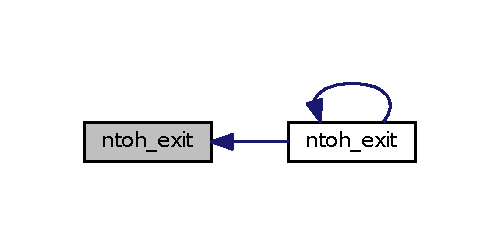
\includegraphics[width=240pt]{namespacelibntoh_ac9165058dd973c10bde158e460e4c9d0_icgraph}
\end{center}
\end{figure}


\hypertarget{namespacelibntoh_a4fc0c3f6a2d347f7b84aa3d14ae1f7ed}{\index{libntoh@{libntoh}!ntoh\-\_\-get\-\_\-errdesc@{ntoh\-\_\-get\-\_\-errdesc}}
\index{ntoh\-\_\-get\-\_\-errdesc@{ntoh\-\_\-get\-\_\-errdesc}!libntoh@{libntoh}}
\subsubsection[{ntoh\-\_\-get\-\_\-errdesc}]{\setlength{\rightskip}{0pt plus 5cm}def libntoh.\-ntoh\-\_\-get\-\_\-errdesc (
\begin{DoxyParamCaption}
\item[{}]{val}
\end{DoxyParamCaption}
)}}\label{namespacelibntoh_a4fc0c3f6a2d347f7b84aa3d14ae1f7ed}
\hypertarget{namespacelibntoh_a768a0989fd47dcb74a6d3bb44351ec99}{\index{libntoh@{libntoh}!ntoh\-\_\-get\-\_\-reason@{ntoh\-\_\-get\-\_\-reason}}
\index{ntoh\-\_\-get\-\_\-reason@{ntoh\-\_\-get\-\_\-reason}!libntoh@{libntoh}}
\subsubsection[{ntoh\-\_\-get\-\_\-reason}]{\setlength{\rightskip}{0pt plus 5cm}def libntoh.\-ntoh\-\_\-get\-\_\-reason (
\begin{DoxyParamCaption}
\item[{}]{val}
\end{DoxyParamCaption}
)}}\label{namespacelibntoh_a768a0989fd47dcb74a6d3bb44351ec99}
\hypertarget{namespacelibntoh_a458eef17394e38c8f98d09b1668485cd}{\index{libntoh@{libntoh}!ntoh\-\_\-get\-\_\-retval\-\_\-desc@{ntoh\-\_\-get\-\_\-retval\-\_\-desc}}
\index{ntoh\-\_\-get\-\_\-retval\-\_\-desc@{ntoh\-\_\-get\-\_\-retval\-\_\-desc}!libntoh@{libntoh}}
\subsubsection[{ntoh\-\_\-get\-\_\-retval\-\_\-desc}]{\setlength{\rightskip}{0pt plus 5cm}def libntoh.\-ntoh\-\_\-get\-\_\-retval\-\_\-desc (
\begin{DoxyParamCaption}
\item[{}]{val}
\end{DoxyParamCaption}
)}}\label{namespacelibntoh_a458eef17394e38c8f98d09b1668485cd}
\hypertarget{namespacelibntoh_ada1514e5ee06acbcbfedd22bb987c069}{\index{libntoh@{libntoh}!ntoh\-\_\-init@{ntoh\-\_\-init}}
\index{ntoh\-\_\-init@{ntoh\-\_\-init}!libntoh@{libntoh}}
\subsubsection[{ntoh\-\_\-init}]{\setlength{\rightskip}{0pt plus 5cm}def libntoh.\-ntoh\-\_\-init (
\begin{DoxyParamCaption}
\item[{void}]{}
\end{DoxyParamCaption}
)}}\label{namespacelibntoh_ada1514e5ee06acbcbfedd22bb987c069}


Initializes the library (T\-C\-P and I\-Pv4) 



Here is the caller graph for this function\-:
\nopagebreak
\begin{figure}[H]
\begin{center}
\leavevmode
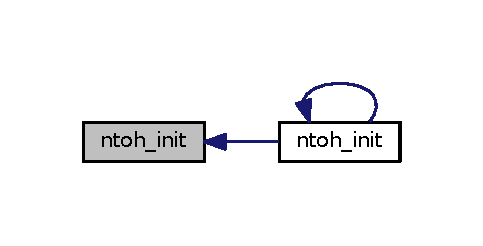
\includegraphics[width=232pt]{namespacelibntoh_ada1514e5ee06acbcbfedd22bb987c069_icgraph}
\end{center}
\end{figure}


\hypertarget{namespacelibntoh_ab8fcc11d5d35ef0f2681782ebe55a748}{\index{libntoh@{libntoh}!ntoh\-\_\-ipv4\-\_\-add\-\_\-fragment@{ntoh\-\_\-ipv4\-\_\-add\-\_\-fragment}}
\index{ntoh\-\_\-ipv4\-\_\-add\-\_\-fragment@{ntoh\-\_\-ipv4\-\_\-add\-\_\-fragment}!libntoh@{libntoh}}
\subsubsection[{ntoh\-\_\-ipv4\-\_\-add\-\_\-fragment}]{\setlength{\rightskip}{0pt plus 5cm}def libntoh.\-ntoh\-\_\-ipv4\-\_\-add\-\_\-fragment (
\begin{DoxyParamCaption}
\item[{}]{session, }
\item[{}]{flow, }
\item[{}]{iphdr, }
\item[{}]{len}
\end{DoxyParamCaption}
)}}\label{namespacelibntoh_ab8fcc11d5d35ef0f2681782ebe55a748}
\hypertarget{namespacelibntoh_a6e344bcc152eb0e83465829d5324b972}{\index{libntoh@{libntoh}!ntoh\-\_\-ipv4\-\_\-count\-\_\-flows@{ntoh\-\_\-ipv4\-\_\-count\-\_\-flows}}
\index{ntoh\-\_\-ipv4\-\_\-count\-\_\-flows@{ntoh\-\_\-ipv4\-\_\-count\-\_\-flows}!libntoh@{libntoh}}
\subsubsection[{ntoh\-\_\-ipv4\-\_\-count\-\_\-flows}]{\setlength{\rightskip}{0pt plus 5cm}def libntoh.\-ntoh\-\_\-ipv4\-\_\-count\-\_\-flows (
\begin{DoxyParamCaption}
\item[{}]{session}
\end{DoxyParamCaption}
)}}\label{namespacelibntoh_a6e344bcc152eb0e83465829d5324b972}
\hypertarget{namespacelibntoh_ab056e87608725bb280228ed713d379cd}{\index{libntoh@{libntoh}!ntoh\-\_\-ipv4\-\_\-exit@{ntoh\-\_\-ipv4\-\_\-exit}}
\index{ntoh\-\_\-ipv4\-\_\-exit@{ntoh\-\_\-ipv4\-\_\-exit}!libntoh@{libntoh}}
\subsubsection[{ntoh\-\_\-ipv4\-\_\-exit}]{\setlength{\rightskip}{0pt plus 5cm}def libntoh.\-ntoh\-\_\-ipv4\-\_\-exit (
\begin{DoxyParamCaption}
\item[{void}]{}
\end{DoxyParamCaption}
)}}\label{namespacelibntoh_ab056e87608725bb280228ed713d379cd}


Flush all I\-Pv4 sessions and release all resources. 



Here is the caller graph for this function\-:
\nopagebreak
\begin{figure}[H]
\begin{center}
\leavevmode
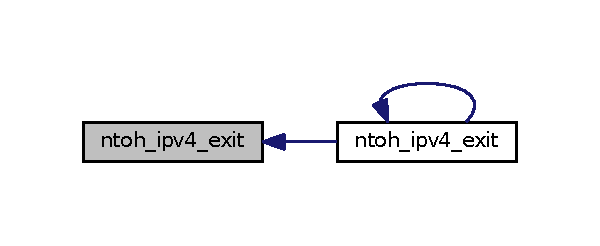
\includegraphics[width=288pt]{namespacelibntoh_ab056e87608725bb280228ed713d379cd_icgraph}
\end{center}
\end{figure}


\hypertarget{namespacelibntoh_a4f6b0a0caa07fd99f6e15fd6cf127226}{\index{libntoh@{libntoh}!ntoh\-\_\-ipv4\-\_\-find\-\_\-flow@{ntoh\-\_\-ipv4\-\_\-find\-\_\-flow}}
\index{ntoh\-\_\-ipv4\-\_\-find\-\_\-flow@{ntoh\-\_\-ipv4\-\_\-find\-\_\-flow}!libntoh@{libntoh}}
\subsubsection[{ntoh\-\_\-ipv4\-\_\-find\-\_\-flow}]{\setlength{\rightskip}{0pt plus 5cm}def libntoh.\-ntoh\-\_\-ipv4\-\_\-find\-\_\-flow (
\begin{DoxyParamCaption}
\item[{}]{session, }
\item[{}]{tuple4}
\end{DoxyParamCaption}
)}}\label{namespacelibntoh_a4f6b0a0caa07fd99f6e15fd6cf127226}
\hypertarget{namespacelibntoh_a0b61fa8f2c49f353882ca66a087f8761}{\index{libntoh@{libntoh}!ntoh\-\_\-ipv4\-\_\-free\-\_\-flow@{ntoh\-\_\-ipv4\-\_\-free\-\_\-flow}}
\index{ntoh\-\_\-ipv4\-\_\-free\-\_\-flow@{ntoh\-\_\-ipv4\-\_\-free\-\_\-flow}!libntoh@{libntoh}}
\subsubsection[{ntoh\-\_\-ipv4\-\_\-free\-\_\-flow}]{\setlength{\rightskip}{0pt plus 5cm}def libntoh.\-ntoh\-\_\-ipv4\-\_\-free\-\_\-flow (
\begin{DoxyParamCaption}
\item[{}]{session, }
\item[{}]{flow, }
\item[{}]{reason}
\end{DoxyParamCaption}
)}}\label{namespacelibntoh_a0b61fa8f2c49f353882ca66a087f8761}
\hypertarget{namespacelibntoh_ae1ba03207cb4ab5e499805d44476d14e}{\index{libntoh@{libntoh}!ntoh\-\_\-ipv4\-\_\-free\-\_\-session@{ntoh\-\_\-ipv4\-\_\-free\-\_\-session}}
\index{ntoh\-\_\-ipv4\-\_\-free\-\_\-session@{ntoh\-\_\-ipv4\-\_\-free\-\_\-session}!libntoh@{libntoh}}
\subsubsection[{ntoh\-\_\-ipv4\-\_\-free\-\_\-session}]{\setlength{\rightskip}{0pt plus 5cm}def libntoh.\-ntoh\-\_\-ipv4\-\_\-free\-\_\-session (
\begin{DoxyParamCaption}
\item[{}]{session}
\end{DoxyParamCaption}
)}}\label{namespacelibntoh_ae1ba03207cb4ab5e499805d44476d14e}
\hypertarget{namespacelibntoh_acfedc8ec47ed540383679d90996fa091}{\index{libntoh@{libntoh}!ntoh\-\_\-ipv4\-\_\-get\-\_\-size@{ntoh\-\_\-ipv4\-\_\-get\-\_\-size}}
\index{ntoh\-\_\-ipv4\-\_\-get\-\_\-size@{ntoh\-\_\-ipv4\-\_\-get\-\_\-size}!libntoh@{libntoh}}
\subsubsection[{ntoh\-\_\-ipv4\-\_\-get\-\_\-size}]{\setlength{\rightskip}{0pt plus 5cm}def libntoh.\-ntoh\-\_\-ipv4\-\_\-get\-\_\-size (
\begin{DoxyParamCaption}
\item[{}]{session}
\end{DoxyParamCaption}
)}}\label{namespacelibntoh_acfedc8ec47ed540383679d90996fa091}
\hypertarget{namespacelibntoh_a043d53b9179d180b046f6d9b1d762bcb}{\index{libntoh@{libntoh}!ntoh\-\_\-ipv4\-\_\-get\-\_\-tuple4@{ntoh\-\_\-ipv4\-\_\-get\-\_\-tuple4}}
\index{ntoh\-\_\-ipv4\-\_\-get\-\_\-tuple4@{ntoh\-\_\-ipv4\-\_\-get\-\_\-tuple4}!libntoh@{libntoh}}
\subsubsection[{ntoh\-\_\-ipv4\-\_\-get\-\_\-tuple4}]{\setlength{\rightskip}{0pt plus 5cm}def libntoh.\-ntoh\-\_\-ipv4\-\_\-get\-\_\-tuple4 (
\begin{DoxyParamCaption}
\item[{}]{ip, }
\item[{}]{tuple}
\end{DoxyParamCaption}
)}}\label{namespacelibntoh_a043d53b9179d180b046f6d9b1d762bcb}
\hypertarget{namespacelibntoh_aba9fb731ee41efde167deffeb7a79bd0}{\index{libntoh@{libntoh}!ntoh\-\_\-ipv4\-\_\-init@{ntoh\-\_\-ipv4\-\_\-init}}
\index{ntoh\-\_\-ipv4\-\_\-init@{ntoh\-\_\-ipv4\-\_\-init}!libntoh@{libntoh}}
\subsubsection[{ntoh\-\_\-ipv4\-\_\-init}]{\setlength{\rightskip}{0pt plus 5cm}def libntoh.\-ntoh\-\_\-ipv4\-\_\-init (
\begin{DoxyParamCaption}
\item[{void}]{}
\end{DoxyParamCaption}
)}}\label{namespacelibntoh_aba9fb731ee41efde167deffeb7a79bd0}


Initializes the I\-Pv4 defragmentation. 



Here is the caller graph for this function\-:
\nopagebreak
\begin{figure}[H]
\begin{center}
\leavevmode
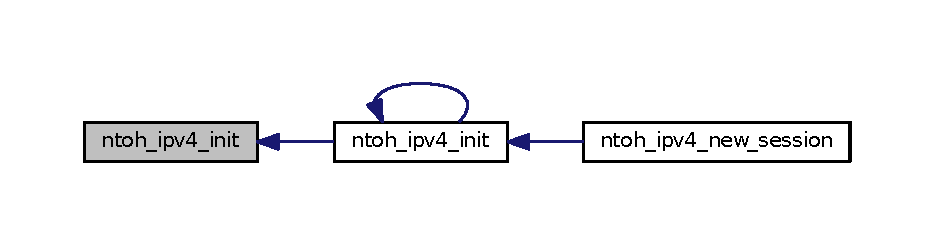
\includegraphics[width=350pt]{namespacelibntoh_aba9fb731ee41efde167deffeb7a79bd0_icgraph}
\end{center}
\end{figure}


\hypertarget{namespacelibntoh_a5ac428789b792a4daac0972f8db83808}{\index{libntoh@{libntoh}!ntoh\-\_\-ipv4\-\_\-new\-\_\-flow@{ntoh\-\_\-ipv4\-\_\-new\-\_\-flow}}
\index{ntoh\-\_\-ipv4\-\_\-new\-\_\-flow@{ntoh\-\_\-ipv4\-\_\-new\-\_\-flow}!libntoh@{libntoh}}
\subsubsection[{ntoh\-\_\-ipv4\-\_\-new\-\_\-flow}]{\setlength{\rightskip}{0pt plus 5cm}def libntoh.\-ntoh\-\_\-ipv4\-\_\-new\-\_\-flow (
\begin{DoxyParamCaption}
\item[{}]{session, }
\item[{}]{tuple4, }
\item[{}]{function, }
\item[{}]{udata, }
\item[{}]{error}
\end{DoxyParamCaption}
)}}\label{namespacelibntoh_a5ac428789b792a4daac0972f8db83808}
\hypertarget{namespacelibntoh_a1be2b34836f25595287826bbea7d0ee7}{\index{libntoh@{libntoh}!ntoh\-\_\-ipv4\-\_\-new\-\_\-session@{ntoh\-\_\-ipv4\-\_\-new\-\_\-session}}
\index{ntoh\-\_\-ipv4\-\_\-new\-\_\-session@{ntoh\-\_\-ipv4\-\_\-new\-\_\-session}!libntoh@{libntoh}}
\subsubsection[{ntoh\-\_\-ipv4\-\_\-new\-\_\-session}]{\setlength{\rightskip}{0pt plus 5cm}def libntoh.\-ntoh\-\_\-ipv4\-\_\-new\-\_\-session (
\begin{DoxyParamCaption}
\item[{}]{max\-\_\-flows, }
\item[{}]{max\-\_\-mem, }
\item[{}]{error}
\end{DoxyParamCaption}
)}}\label{namespacelibntoh_a1be2b34836f25595287826bbea7d0ee7}
\hypertarget{namespacelibntoh_a0eed2a936073a47a22f45b52a0a9919a}{\index{libntoh@{libntoh}!ntoh\-\_\-ipv6\-\_\-add\-\_\-fragment@{ntoh\-\_\-ipv6\-\_\-add\-\_\-fragment}}
\index{ntoh\-\_\-ipv6\-\_\-add\-\_\-fragment@{ntoh\-\_\-ipv6\-\_\-add\-\_\-fragment}!libntoh@{libntoh}}
\subsubsection[{ntoh\-\_\-ipv6\-\_\-add\-\_\-fragment}]{\setlength{\rightskip}{0pt plus 5cm}def libntoh.\-ntoh\-\_\-ipv6\-\_\-add\-\_\-fragment (
\begin{DoxyParamCaption}
\item[{}]{session, }
\item[{}]{flow, }
\item[{}]{iphdr, }
\item[{}]{len}
\end{DoxyParamCaption}
)}}\label{namespacelibntoh_a0eed2a936073a47a22f45b52a0a9919a}
\hypertarget{namespacelibntoh_a286fe15393f1999d64fb2dd0a5a8e7b3}{\index{libntoh@{libntoh}!ntoh\-\_\-ipv6\-\_\-count\-\_\-flows@{ntoh\-\_\-ipv6\-\_\-count\-\_\-flows}}
\index{ntoh\-\_\-ipv6\-\_\-count\-\_\-flows@{ntoh\-\_\-ipv6\-\_\-count\-\_\-flows}!libntoh@{libntoh}}
\subsubsection[{ntoh\-\_\-ipv6\-\_\-count\-\_\-flows}]{\setlength{\rightskip}{0pt plus 5cm}def libntoh.\-ntoh\-\_\-ipv6\-\_\-count\-\_\-flows (
\begin{DoxyParamCaption}
\item[{}]{session}
\end{DoxyParamCaption}
)}}\label{namespacelibntoh_a286fe15393f1999d64fb2dd0a5a8e7b3}
\hypertarget{namespacelibntoh_a97fd0b045bb722630083c7f33be1692c}{\index{libntoh@{libntoh}!ntoh\-\_\-ipv6\-\_\-exit@{ntoh\-\_\-ipv6\-\_\-exit}}
\index{ntoh\-\_\-ipv6\-\_\-exit@{ntoh\-\_\-ipv6\-\_\-exit}!libntoh@{libntoh}}
\subsubsection[{ntoh\-\_\-ipv6\-\_\-exit}]{\setlength{\rightskip}{0pt plus 5cm}def libntoh.\-ntoh\-\_\-ipv6\-\_\-exit (
\begin{DoxyParamCaption}
\item[{void}]{}
\end{DoxyParamCaption}
)}}\label{namespacelibntoh_a97fd0b045bb722630083c7f33be1692c}


Flush all I\-Pv6 sessions and release all resources. 



Here is the caller graph for this function\-:
\nopagebreak
\begin{figure}[H]
\begin{center}
\leavevmode
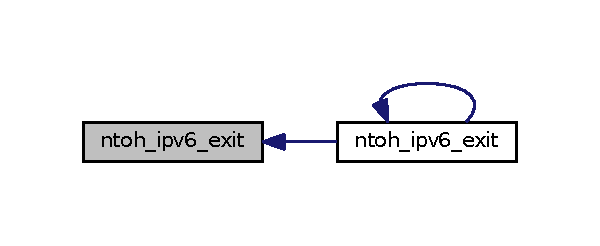
\includegraphics[width=288pt]{namespacelibntoh_a97fd0b045bb722630083c7f33be1692c_icgraph}
\end{center}
\end{figure}


\hypertarget{namespacelibntoh_a19c219b9e6fc394a6fe3a2f195e5510e}{\index{libntoh@{libntoh}!ntoh\-\_\-ipv6\-\_\-find\-\_\-flow@{ntoh\-\_\-ipv6\-\_\-find\-\_\-flow}}
\index{ntoh\-\_\-ipv6\-\_\-find\-\_\-flow@{ntoh\-\_\-ipv6\-\_\-find\-\_\-flow}!libntoh@{libntoh}}
\subsubsection[{ntoh\-\_\-ipv6\-\_\-find\-\_\-flow}]{\setlength{\rightskip}{0pt plus 5cm}def libntoh.\-ntoh\-\_\-ipv6\-\_\-find\-\_\-flow (
\begin{DoxyParamCaption}
\item[{}]{session, }
\item[{}]{tuple4}
\end{DoxyParamCaption}
)}}\label{namespacelibntoh_a19c219b9e6fc394a6fe3a2f195e5510e}
\hypertarget{namespacelibntoh_aba58e6cfb09e216baf71533f5d39b9f1}{\index{libntoh@{libntoh}!ntoh\-\_\-ipv6\-\_\-free\-\_\-flow@{ntoh\-\_\-ipv6\-\_\-free\-\_\-flow}}
\index{ntoh\-\_\-ipv6\-\_\-free\-\_\-flow@{ntoh\-\_\-ipv6\-\_\-free\-\_\-flow}!libntoh@{libntoh}}
\subsubsection[{ntoh\-\_\-ipv6\-\_\-free\-\_\-flow}]{\setlength{\rightskip}{0pt plus 5cm}def libntoh.\-ntoh\-\_\-ipv6\-\_\-free\-\_\-flow (
\begin{DoxyParamCaption}
\item[{}]{session, }
\item[{}]{flow, }
\item[{}]{reason}
\end{DoxyParamCaption}
)}}\label{namespacelibntoh_aba58e6cfb09e216baf71533f5d39b9f1}
\hypertarget{namespacelibntoh_ae78241e2e3b8862c2f40db63b17e8982}{\index{libntoh@{libntoh}!ntoh\-\_\-ipv6\-\_\-free\-\_\-session@{ntoh\-\_\-ipv6\-\_\-free\-\_\-session}}
\index{ntoh\-\_\-ipv6\-\_\-free\-\_\-session@{ntoh\-\_\-ipv6\-\_\-free\-\_\-session}!libntoh@{libntoh}}
\subsubsection[{ntoh\-\_\-ipv6\-\_\-free\-\_\-session}]{\setlength{\rightskip}{0pt plus 5cm}def libntoh.\-ntoh\-\_\-ipv6\-\_\-free\-\_\-session (
\begin{DoxyParamCaption}
\item[{}]{session}
\end{DoxyParamCaption}
)}}\label{namespacelibntoh_ae78241e2e3b8862c2f40db63b17e8982}
\hypertarget{namespacelibntoh_ab1c0121c082a2f0ba29aed397447645a}{\index{libntoh@{libntoh}!ntoh\-\_\-ipv6\-\_\-get\-\_\-size@{ntoh\-\_\-ipv6\-\_\-get\-\_\-size}}
\index{ntoh\-\_\-ipv6\-\_\-get\-\_\-size@{ntoh\-\_\-ipv6\-\_\-get\-\_\-size}!libntoh@{libntoh}}
\subsubsection[{ntoh\-\_\-ipv6\-\_\-get\-\_\-size}]{\setlength{\rightskip}{0pt plus 5cm}def libntoh.\-ntoh\-\_\-ipv6\-\_\-get\-\_\-size (
\begin{DoxyParamCaption}
\item[{}]{session}
\end{DoxyParamCaption}
)}}\label{namespacelibntoh_ab1c0121c082a2f0ba29aed397447645a}
\hypertarget{namespacelibntoh_a3213f1c82559f01940932603f2432f6b}{\index{libntoh@{libntoh}!ntoh\-\_\-ipv6\-\_\-get\-\_\-tuple4@{ntoh\-\_\-ipv6\-\_\-get\-\_\-tuple4}}
\index{ntoh\-\_\-ipv6\-\_\-get\-\_\-tuple4@{ntoh\-\_\-ipv6\-\_\-get\-\_\-tuple4}!libntoh@{libntoh}}
\subsubsection[{ntoh\-\_\-ipv6\-\_\-get\-\_\-tuple4}]{\setlength{\rightskip}{0pt plus 5cm}def libntoh.\-ntoh\-\_\-ipv6\-\_\-get\-\_\-tuple4 (
\begin{DoxyParamCaption}
\item[{}]{ip, }
\item[{}]{tuple}
\end{DoxyParamCaption}
)}}\label{namespacelibntoh_a3213f1c82559f01940932603f2432f6b}
\hypertarget{namespacelibntoh_a808b2d917189ed6635c33be8db53369e}{\index{libntoh@{libntoh}!ntoh\-\_\-ipv6\-\_\-init@{ntoh\-\_\-ipv6\-\_\-init}}
\index{ntoh\-\_\-ipv6\-\_\-init@{ntoh\-\_\-ipv6\-\_\-init}!libntoh@{libntoh}}
\subsubsection[{ntoh\-\_\-ipv6\-\_\-init}]{\setlength{\rightskip}{0pt plus 5cm}def libntoh.\-ntoh\-\_\-ipv6\-\_\-init (
\begin{DoxyParamCaption}
\item[{void}]{}
\end{DoxyParamCaption}
)}}\label{namespacelibntoh_a808b2d917189ed6635c33be8db53369e}


Initializes the I\-Pv6 defragmentation. 



Here is the caller graph for this function\-:
\nopagebreak
\begin{figure}[H]
\begin{center}
\leavevmode
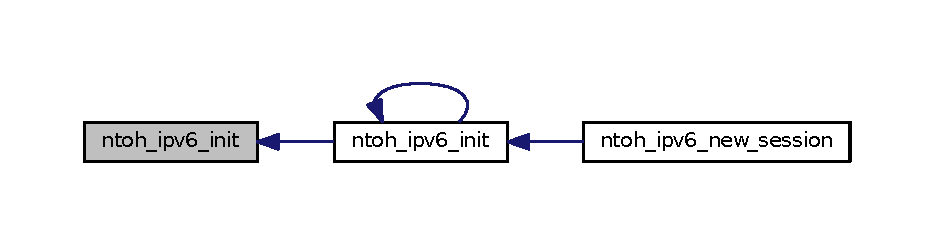
\includegraphics[width=350pt]{namespacelibntoh_a808b2d917189ed6635c33be8db53369e_icgraph}
\end{center}
\end{figure}


\hypertarget{namespacelibntoh_a1e72977ec4478820d6d18da1a4143455}{\index{libntoh@{libntoh}!ntoh\-\_\-ipv6\-\_\-new\-\_\-flow@{ntoh\-\_\-ipv6\-\_\-new\-\_\-flow}}
\index{ntoh\-\_\-ipv6\-\_\-new\-\_\-flow@{ntoh\-\_\-ipv6\-\_\-new\-\_\-flow}!libntoh@{libntoh}}
\subsubsection[{ntoh\-\_\-ipv6\-\_\-new\-\_\-flow}]{\setlength{\rightskip}{0pt plus 5cm}def libntoh.\-ntoh\-\_\-ipv6\-\_\-new\-\_\-flow (
\begin{DoxyParamCaption}
\item[{}]{session, }
\item[{}]{tuple4, }
\item[{}]{function, }
\item[{}]{udata, }
\item[{}]{error}
\end{DoxyParamCaption}
)}}\label{namespacelibntoh_a1e72977ec4478820d6d18da1a4143455}
\hypertarget{namespacelibntoh_a68c9889ffb2bf2240ca3ae27a75789b4}{\index{libntoh@{libntoh}!ntoh\-\_\-ipv6\-\_\-new\-\_\-session@{ntoh\-\_\-ipv6\-\_\-new\-\_\-session}}
\index{ntoh\-\_\-ipv6\-\_\-new\-\_\-session@{ntoh\-\_\-ipv6\-\_\-new\-\_\-session}!libntoh@{libntoh}}
\subsubsection[{ntoh\-\_\-ipv6\-\_\-new\-\_\-session}]{\setlength{\rightskip}{0pt plus 5cm}def libntoh.\-ntoh\-\_\-ipv6\-\_\-new\-\_\-session (
\begin{DoxyParamCaption}
\item[{}]{max\-\_\-flows, }
\item[{}]{max\-\_\-mem, }
\item[{}]{error}
\end{DoxyParamCaption}
)}}\label{namespacelibntoh_a68c9889ffb2bf2240ca3ae27a75789b4}
\hypertarget{namespacelibntoh_aa11d3df7f8e96c97e8b94817fbdf2c91}{\index{libntoh@{libntoh}!ntoh\-\_\-tcp\-\_\-add\-\_\-segment@{ntoh\-\_\-tcp\-\_\-add\-\_\-segment}}
\index{ntoh\-\_\-tcp\-\_\-add\-\_\-segment@{ntoh\-\_\-tcp\-\_\-add\-\_\-segment}!libntoh@{libntoh}}
\subsubsection[{ntoh\-\_\-tcp\-\_\-add\-\_\-segment}]{\setlength{\rightskip}{0pt plus 5cm}def libntoh.\-ntoh\-\_\-tcp\-\_\-add\-\_\-segment (
\begin{DoxyParamCaption}
\item[{}]{session, }
\item[{}]{stream, }
\item[{}]{ip, }
\item[{}]{len, }
\item[{}]{udata}
\end{DoxyParamCaption}
)}}\label{namespacelibntoh_aa11d3df7f8e96c97e8b94817fbdf2c91}
\hypertarget{namespacelibntoh_a862d19498bcb4d0485393cf13d2e1ced}{\index{libntoh@{libntoh}!ntoh\-\_\-tcp\-\_\-count\-\_\-streams@{ntoh\-\_\-tcp\-\_\-count\-\_\-streams}}
\index{ntoh\-\_\-tcp\-\_\-count\-\_\-streams@{ntoh\-\_\-tcp\-\_\-count\-\_\-streams}!libntoh@{libntoh}}
\subsubsection[{ntoh\-\_\-tcp\-\_\-count\-\_\-streams}]{\setlength{\rightskip}{0pt plus 5cm}def libntoh.\-ntoh\-\_\-tcp\-\_\-count\-\_\-streams (
\begin{DoxyParamCaption}
\item[{}]{session}
\end{DoxyParamCaption}
)}}\label{namespacelibntoh_a862d19498bcb4d0485393cf13d2e1ced}
\hypertarget{namespacelibntoh_a213a19bc5e7f81d861aa0784ed68a805}{\index{libntoh@{libntoh}!ntoh\-\_\-tcp\-\_\-exit@{ntoh\-\_\-tcp\-\_\-exit}}
\index{ntoh\-\_\-tcp\-\_\-exit@{ntoh\-\_\-tcp\-\_\-exit}!libntoh@{libntoh}}
\subsubsection[{ntoh\-\_\-tcp\-\_\-exit}]{\setlength{\rightskip}{0pt plus 5cm}def libntoh.\-ntoh\-\_\-tcp\-\_\-exit (
\begin{DoxyParamCaption}
\item[{void}]{}
\end{DoxyParamCaption}
)}}\label{namespacelibntoh_a213a19bc5e7f81d861aa0784ed68a805}


Releases all resources used by T\-C\-P reassembly. 



Here is the caller graph for this function\-:
\nopagebreak
\begin{figure}[H]
\begin{center}
\leavevmode
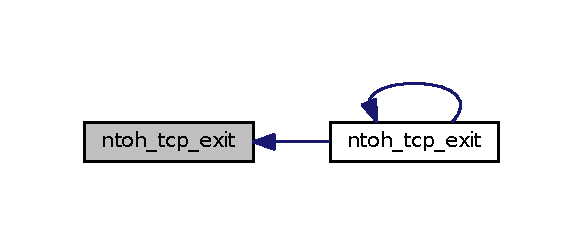
\includegraphics[width=280pt]{namespacelibntoh_a213a19bc5e7f81d861aa0784ed68a805_icgraph}
\end{center}
\end{figure}


\hypertarget{namespacelibntoh_a8a187ac0b9c8fd2bb6148125c9c2e66a}{\index{libntoh@{libntoh}!ntoh\-\_\-tcp\-\_\-find\-\_\-stream@{ntoh\-\_\-tcp\-\_\-find\-\_\-stream}}
\index{ntoh\-\_\-tcp\-\_\-find\-\_\-stream@{ntoh\-\_\-tcp\-\_\-find\-\_\-stream}!libntoh@{libntoh}}
\subsubsection[{ntoh\-\_\-tcp\-\_\-find\-\_\-stream}]{\setlength{\rightskip}{0pt plus 5cm}def libntoh.\-ntoh\-\_\-tcp\-\_\-find\-\_\-stream (
\begin{DoxyParamCaption}
\item[{}]{session, }
\item[{}]{tuple5}
\end{DoxyParamCaption}
)}}\label{namespacelibntoh_a8a187ac0b9c8fd2bb6148125c9c2e66a}
\hypertarget{namespacelibntoh_a8e7ef018eced57f8aec0a1576038944b}{\index{libntoh@{libntoh}!ntoh\-\_\-tcp\-\_\-free\-\_\-session@{ntoh\-\_\-tcp\-\_\-free\-\_\-session}}
\index{ntoh\-\_\-tcp\-\_\-free\-\_\-session@{ntoh\-\_\-tcp\-\_\-free\-\_\-session}!libntoh@{libntoh}}
\subsubsection[{ntoh\-\_\-tcp\-\_\-free\-\_\-session}]{\setlength{\rightskip}{0pt plus 5cm}def libntoh.\-ntoh\-\_\-tcp\-\_\-free\-\_\-session (
\begin{DoxyParamCaption}
\item[{}]{session}
\end{DoxyParamCaption}
)}}\label{namespacelibntoh_a8e7ef018eced57f8aec0a1576038944b}
\hypertarget{namespacelibntoh_aa6b25cb06f262251c7f210c4949f13f2}{\index{libntoh@{libntoh}!ntoh\-\_\-tcp\-\_\-free\-\_\-stream@{ntoh\-\_\-tcp\-\_\-free\-\_\-stream}}
\index{ntoh\-\_\-tcp\-\_\-free\-\_\-stream@{ntoh\-\_\-tcp\-\_\-free\-\_\-stream}!libntoh@{libntoh}}
\subsubsection[{ntoh\-\_\-tcp\-\_\-free\-\_\-stream}]{\setlength{\rightskip}{0pt plus 5cm}def libntoh.\-ntoh\-\_\-tcp\-\_\-free\-\_\-stream (
\begin{DoxyParamCaption}
\item[{}]{session, }
\item[{}]{stream, }
\item[{}]{reason, }
\item[{}]{extra}
\end{DoxyParamCaption}
)}}\label{namespacelibntoh_aa6b25cb06f262251c7f210c4949f13f2}
\hypertarget{namespacelibntoh_a981426ebc5be1a01b035a71f56e03113}{\index{libntoh@{libntoh}!ntoh\-\_\-tcp\-\_\-get\-\_\-size@{ntoh\-\_\-tcp\-\_\-get\-\_\-size}}
\index{ntoh\-\_\-tcp\-\_\-get\-\_\-size@{ntoh\-\_\-tcp\-\_\-get\-\_\-size}!libntoh@{libntoh}}
\subsubsection[{ntoh\-\_\-tcp\-\_\-get\-\_\-size}]{\setlength{\rightskip}{0pt plus 5cm}def libntoh.\-ntoh\-\_\-tcp\-\_\-get\-\_\-size (
\begin{DoxyParamCaption}
\item[{}]{session}
\end{DoxyParamCaption}
)}}\label{namespacelibntoh_a981426ebc5be1a01b035a71f56e03113}
\hypertarget{namespacelibntoh_aa6f3eae9edf20f33cbddcee20be23bbb}{\index{libntoh@{libntoh}!ntoh\-\_\-tcp\-\_\-get\-\_\-status@{ntoh\-\_\-tcp\-\_\-get\-\_\-status}}
\index{ntoh\-\_\-tcp\-\_\-get\-\_\-status@{ntoh\-\_\-tcp\-\_\-get\-\_\-status}!libntoh@{libntoh}}
\subsubsection[{ntoh\-\_\-tcp\-\_\-get\-\_\-status}]{\setlength{\rightskip}{0pt plus 5cm}def libntoh.\-ntoh\-\_\-tcp\-\_\-get\-\_\-status (
\begin{DoxyParamCaption}
\item[{}]{status}
\end{DoxyParamCaption}
)}}\label{namespacelibntoh_aa6f3eae9edf20f33cbddcee20be23bbb}
\hypertarget{namespacelibntoh_ad7bb9b76e72995ea8c9de3630a671cb4}{\index{libntoh@{libntoh}!ntoh\-\_\-tcp\-\_\-get\-\_\-tuple5@{ntoh\-\_\-tcp\-\_\-get\-\_\-tuple5}}
\index{ntoh\-\_\-tcp\-\_\-get\-\_\-tuple5@{ntoh\-\_\-tcp\-\_\-get\-\_\-tuple5}!libntoh@{libntoh}}
\subsubsection[{ntoh\-\_\-tcp\-\_\-get\-\_\-tuple5}]{\setlength{\rightskip}{0pt plus 5cm}def libntoh.\-ntoh\-\_\-tcp\-\_\-get\-\_\-tuple5 (
\begin{DoxyParamCaption}
\item[{}]{ip, }
\item[{}]{tcp, }
\item[{}]{tuple}
\end{DoxyParamCaption}
)}}\label{namespacelibntoh_ad7bb9b76e72995ea8c9de3630a671cb4}
\hypertarget{namespacelibntoh_a0ac2c174ee2faef679c1d5fc56a5a439}{\index{libntoh@{libntoh}!ntoh\-\_\-tcp\-\_\-init@{ntoh\-\_\-tcp\-\_\-init}}
\index{ntoh\-\_\-tcp\-\_\-init@{ntoh\-\_\-tcp\-\_\-init}!libntoh@{libntoh}}
\subsubsection[{ntoh\-\_\-tcp\-\_\-init}]{\setlength{\rightskip}{0pt plus 5cm}def libntoh.\-ntoh\-\_\-tcp\-\_\-init (
\begin{DoxyParamCaption}
\item[{void}]{}
\end{DoxyParamCaption}
)}}\label{namespacelibntoh_a0ac2c174ee2faef679c1d5fc56a5a439}


Initializes all needed resources for T\-C\-P reassembly. 



Here is the caller graph for this function\-:
\nopagebreak
\begin{figure}[H]
\begin{center}
\leavevmode
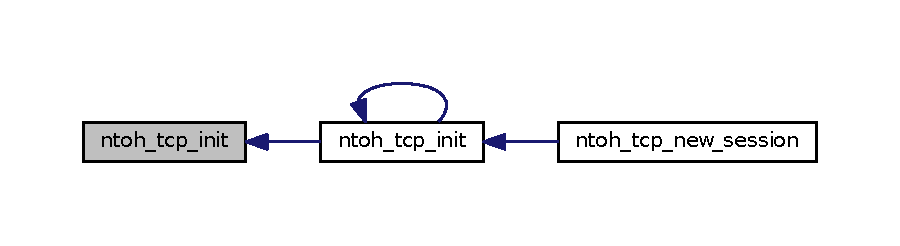
\includegraphics[width=350pt]{namespacelibntoh_a0ac2c174ee2faef679c1d5fc56a5a439_icgraph}
\end{center}
\end{figure}


\hypertarget{namespacelibntoh_a62260d771e3186e3e59f96859249a121}{\index{libntoh@{libntoh}!ntoh\-\_\-tcp\-\_\-new\-\_\-session@{ntoh\-\_\-tcp\-\_\-new\-\_\-session}}
\index{ntoh\-\_\-tcp\-\_\-new\-\_\-session@{ntoh\-\_\-tcp\-\_\-new\-\_\-session}!libntoh@{libntoh}}
\subsubsection[{ntoh\-\_\-tcp\-\_\-new\-\_\-session}]{\setlength{\rightskip}{0pt plus 5cm}def libntoh.\-ntoh\-\_\-tcp\-\_\-new\-\_\-session (
\begin{DoxyParamCaption}
\item[{}]{max\-\_\-streams, }
\item[{}]{max\-\_\-timewait, }
\item[{}]{error}
\end{DoxyParamCaption}
)}}\label{namespacelibntoh_a62260d771e3186e3e59f96859249a121}
\hypertarget{namespacelibntoh_a436bf66ce9902fbbff543582d1771760}{\index{libntoh@{libntoh}!ntoh\-\_\-tcp\-\_\-new\-\_\-stream@{ntoh\-\_\-tcp\-\_\-new\-\_\-stream}}
\index{ntoh\-\_\-tcp\-\_\-new\-\_\-stream@{ntoh\-\_\-tcp\-\_\-new\-\_\-stream}!libntoh@{libntoh}}
\subsubsection[{ntoh\-\_\-tcp\-\_\-new\-\_\-stream}]{\setlength{\rightskip}{0pt plus 5cm}def libntoh.\-ntoh\-\_\-tcp\-\_\-new\-\_\-stream (
\begin{DoxyParamCaption}
\item[{}]{session, }
\item[{}]{tuple5, }
\item[{}]{function, }
\item[{}]{udata, }
\item[{}]{error, }
\item[{}]{enable\-\_\-check\-\_\-timeout, }
\item[{}]{enable\-\_\-check\-\_\-nowindow}
\end{DoxyParamCaption}
)}}\label{namespacelibntoh_a436bf66ce9902fbbff543582d1771760}
\hypertarget{namespacelibntoh_aaac2d93f6819e10075e65ad7a5eb6e9d}{\index{libntoh@{libntoh}!ntoh\-\_\-version@{ntoh\-\_\-version}}
\index{ntoh\-\_\-version@{ntoh\-\_\-version}!libntoh@{libntoh}}
\subsubsection[{ntoh\-\_\-version}]{\setlength{\rightskip}{0pt plus 5cm}def libntoh.\-ntoh\-\_\-version (
\begin{DoxyParamCaption}
\item[{void}]{}
\end{DoxyParamCaption}
)}}\label{namespacelibntoh_aaac2d93f6819e10075e65ad7a5eb6e9d}


Header files. 

Returns library version \begin{DoxyReturn}{Returns}
The version of the library 
\end{DoxyReturn}


Here is the caller graph for this function\-:
\nopagebreak
\begin{figure}[H]
\begin{center}
\leavevmode
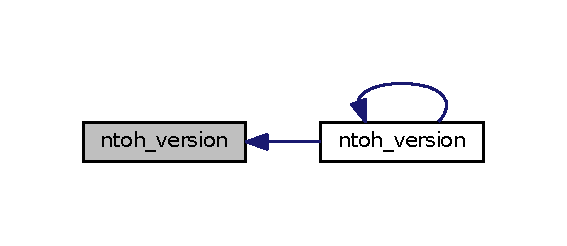
\includegraphics[width=272pt]{namespacelibntoh_aaac2d93f6819e10075e65ad7a5eb6e9d_icgraph}
\end{center}
\end{figure}


\hypertarget{namespacelibntoh_a64cebc095c211e7679d6fe8b466a3c94}{\index{libntoh@{libntoh}!sfhash\-\_\-3words@{sfhash\-\_\-3words}}
\index{sfhash\-\_\-3words@{sfhash\-\_\-3words}!libntoh@{libntoh}}
\subsubsection[{sfhash\-\_\-3words}]{\setlength{\rightskip}{0pt plus 5cm}def libntoh.\-sfhash\-\_\-3words (
\begin{DoxyParamCaption}
\item[{}]{a, }
\item[{}]{b, }
\item[{}]{c, }
\item[{}]{initval}
\end{DoxyParamCaption}
)}}\label{namespacelibntoh_a64cebc095c211e7679d6fe8b466a3c94}
\hypertarget{namespacelibntoh_a20a40d2e70bce861f694525f66632730}{\index{libntoh@{libntoh}!swig\-\_\-import\-\_\-helper@{swig\-\_\-import\-\_\-helper}}
\index{swig\-\_\-import\-\_\-helper@{swig\-\_\-import\-\_\-helper}!libntoh@{libntoh}}
\subsubsection[{swig\-\_\-import\-\_\-helper}]{\setlength{\rightskip}{0pt plus 5cm}def libntoh.\-swig\-\_\-import\-\_\-helper (
\begin{DoxyParamCaption}
{}
\end{DoxyParamCaption}
)}}\label{namespacelibntoh_a20a40d2e70bce861f694525f66632730}
\hypertarget{namespacelibntoh_a34e2d83b0791206e6d7bba25e2c28c7d}{\index{libntoh@{libntoh}!unlock\-\_\-access@{unlock\-\_\-access}}
\index{unlock\-\_\-access@{unlock\-\_\-access}!libntoh@{libntoh}}
\subsubsection[{unlock\-\_\-access}]{\setlength{\rightskip}{0pt plus 5cm}def libntoh.\-unlock\-\_\-access (
\begin{DoxyParamCaption}
\item[{}]{lock}
\end{DoxyParamCaption}
)}}\label{namespacelibntoh_a34e2d83b0791206e6d7bba25e2c28c7d}


\subsection{Variable Documentation}
\hypertarget{namespacelibntoh_ac7d41d0284cbda5058b8afb092a3c22b}{\index{libntoh@{libntoh}!\-\_\-libntoh@{\-\_\-libntoh}}
\index{\-\_\-libntoh@{\-\_\-libntoh}!libntoh@{libntoh}}
\subsubsection[{\-\_\-libntoh}]{\setlength{\rightskip}{0pt plus 5cm}tuple \-\_\-libntoh = {\bf swig\-\_\-import\-\_\-helper}()}}\label{namespacelibntoh_ac7d41d0284cbda5058b8afb092a3c22b}
\hypertarget{namespacelibntoh_a731bbb8755dba80a3e78782d848615a2}{\index{libntoh@{libntoh}!D\-E\-F\-A\-U\-L\-T\-\_\-\-I\-P\-V4\-\_\-\-F\-R\-A\-G\-M\-E\-N\-T\-\_\-\-T\-I\-M\-E\-O\-U\-T@{D\-E\-F\-A\-U\-L\-T\-\_\-\-I\-P\-V4\-\_\-\-F\-R\-A\-G\-M\-E\-N\-T\-\_\-\-T\-I\-M\-E\-O\-U\-T}}
\index{D\-E\-F\-A\-U\-L\-T\-\_\-\-I\-P\-V4\-\_\-\-F\-R\-A\-G\-M\-E\-N\-T\-\_\-\-T\-I\-M\-E\-O\-U\-T@{D\-E\-F\-A\-U\-L\-T\-\_\-\-I\-P\-V4\-\_\-\-F\-R\-A\-G\-M\-E\-N\-T\-\_\-\-T\-I\-M\-E\-O\-U\-T}!libntoh@{libntoh}}
\subsubsection[{D\-E\-F\-A\-U\-L\-T\-\_\-\-I\-P\-V4\-\_\-\-F\-R\-A\-G\-M\-E\-N\-T\-\_\-\-T\-I\-M\-E\-O\-U\-T}]{\setlength{\rightskip}{0pt plus 5cm}D\-E\-F\-A\-U\-L\-T\-\_\-\-I\-P\-V4\-\_\-\-F\-R\-A\-G\-M\-E\-N\-T\-\_\-\-T\-I\-M\-E\-O\-U\-T = \-\_\-libntoh.\-D\-E\-F\-A\-U\-L\-T\-\_\-\-I\-P\-V4\-\_\-\-F\-R\-A\-G\-M\-E\-N\-T\-\_\-\-T\-I\-M\-E\-O\-U\-T}}\label{namespacelibntoh_a731bbb8755dba80a3e78782d848615a2}
\hypertarget{namespacelibntoh_a12e9b7d82d8b14f9a1df42f0790c5e29}{\index{libntoh@{libntoh}!D\-E\-F\-A\-U\-L\-T\-\_\-\-I\-P\-V4\-\_\-\-M\-A\-X\-\_\-\-F\-L\-O\-W\-S@{D\-E\-F\-A\-U\-L\-T\-\_\-\-I\-P\-V4\-\_\-\-M\-A\-X\-\_\-\-F\-L\-O\-W\-S}}
\index{D\-E\-F\-A\-U\-L\-T\-\_\-\-I\-P\-V4\-\_\-\-M\-A\-X\-\_\-\-F\-L\-O\-W\-S@{D\-E\-F\-A\-U\-L\-T\-\_\-\-I\-P\-V4\-\_\-\-M\-A\-X\-\_\-\-F\-L\-O\-W\-S}!libntoh@{libntoh}}
\subsubsection[{D\-E\-F\-A\-U\-L\-T\-\_\-\-I\-P\-V4\-\_\-\-M\-A\-X\-\_\-\-F\-L\-O\-W\-S}]{\setlength{\rightskip}{0pt plus 5cm}D\-E\-F\-A\-U\-L\-T\-\_\-\-I\-P\-V4\-\_\-\-M\-A\-X\-\_\-\-F\-L\-O\-W\-S = \-\_\-libntoh.\-D\-E\-F\-A\-U\-L\-T\-\_\-\-I\-P\-V4\-\_\-\-M\-A\-X\-\_\-\-F\-L\-O\-W\-S}}\label{namespacelibntoh_a12e9b7d82d8b14f9a1df42f0790c5e29}
\hypertarget{namespacelibntoh_a48aa3979830d824db5ae0119843cb508}{\index{libntoh@{libntoh}!D\-E\-F\-A\-U\-L\-T\-\_\-\-I\-P\-V6\-\_\-\-F\-R\-A\-G\-M\-E\-N\-T\-\_\-\-T\-I\-M\-E\-O\-U\-T@{D\-E\-F\-A\-U\-L\-T\-\_\-\-I\-P\-V6\-\_\-\-F\-R\-A\-G\-M\-E\-N\-T\-\_\-\-T\-I\-M\-E\-O\-U\-T}}
\index{D\-E\-F\-A\-U\-L\-T\-\_\-\-I\-P\-V6\-\_\-\-F\-R\-A\-G\-M\-E\-N\-T\-\_\-\-T\-I\-M\-E\-O\-U\-T@{D\-E\-F\-A\-U\-L\-T\-\_\-\-I\-P\-V6\-\_\-\-F\-R\-A\-G\-M\-E\-N\-T\-\_\-\-T\-I\-M\-E\-O\-U\-T}!libntoh@{libntoh}}
\subsubsection[{D\-E\-F\-A\-U\-L\-T\-\_\-\-I\-P\-V6\-\_\-\-F\-R\-A\-G\-M\-E\-N\-T\-\_\-\-T\-I\-M\-E\-O\-U\-T}]{\setlength{\rightskip}{0pt plus 5cm}D\-E\-F\-A\-U\-L\-T\-\_\-\-I\-P\-V6\-\_\-\-F\-R\-A\-G\-M\-E\-N\-T\-\_\-\-T\-I\-M\-E\-O\-U\-T = \-\_\-libntoh.\-D\-E\-F\-A\-U\-L\-T\-\_\-\-I\-P\-V6\-\_\-\-F\-R\-A\-G\-M\-E\-N\-T\-\_\-\-T\-I\-M\-E\-O\-U\-T}}\label{namespacelibntoh_a48aa3979830d824db5ae0119843cb508}
\hypertarget{namespacelibntoh_ad45951b70a3812f517f374be95af60c0}{\index{libntoh@{libntoh}!D\-E\-F\-A\-U\-L\-T\-\_\-\-I\-P\-V6\-\_\-\-M\-A\-X\-\_\-\-F\-L\-O\-W\-S@{D\-E\-F\-A\-U\-L\-T\-\_\-\-I\-P\-V6\-\_\-\-M\-A\-X\-\_\-\-F\-L\-O\-W\-S}}
\index{D\-E\-F\-A\-U\-L\-T\-\_\-\-I\-P\-V6\-\_\-\-M\-A\-X\-\_\-\-F\-L\-O\-W\-S@{D\-E\-F\-A\-U\-L\-T\-\_\-\-I\-P\-V6\-\_\-\-M\-A\-X\-\_\-\-F\-L\-O\-W\-S}!libntoh@{libntoh}}
\subsubsection[{D\-E\-F\-A\-U\-L\-T\-\_\-\-I\-P\-V6\-\_\-\-M\-A\-X\-\_\-\-F\-L\-O\-W\-S}]{\setlength{\rightskip}{0pt plus 5cm}D\-E\-F\-A\-U\-L\-T\-\_\-\-I\-P\-V6\-\_\-\-M\-A\-X\-\_\-\-F\-L\-O\-W\-S = \-\_\-libntoh.\-D\-E\-F\-A\-U\-L\-T\-\_\-\-I\-P\-V6\-\_\-\-M\-A\-X\-\_\-\-F\-L\-O\-W\-S}}\label{namespacelibntoh_ad45951b70a3812f517f374be95af60c0}
\hypertarget{namespacelibntoh_afbc0e8c5bad6756e09f1a0727e686156}{\index{libntoh@{libntoh}!D\-E\-F\-A\-U\-L\-T\-\_\-\-T\-C\-P\-\_\-\-E\-S\-T\-A\-B\-L\-I\-S\-H\-E\-D\-\_\-\-T\-I\-M\-E\-O\-U\-T@{D\-E\-F\-A\-U\-L\-T\-\_\-\-T\-C\-P\-\_\-\-E\-S\-T\-A\-B\-L\-I\-S\-H\-E\-D\-\_\-\-T\-I\-M\-E\-O\-U\-T}}
\index{D\-E\-F\-A\-U\-L\-T\-\_\-\-T\-C\-P\-\_\-\-E\-S\-T\-A\-B\-L\-I\-S\-H\-E\-D\-\_\-\-T\-I\-M\-E\-O\-U\-T@{D\-E\-F\-A\-U\-L\-T\-\_\-\-T\-C\-P\-\_\-\-E\-S\-T\-A\-B\-L\-I\-S\-H\-E\-D\-\_\-\-T\-I\-M\-E\-O\-U\-T}!libntoh@{libntoh}}
\subsubsection[{D\-E\-F\-A\-U\-L\-T\-\_\-\-T\-C\-P\-\_\-\-E\-S\-T\-A\-B\-L\-I\-S\-H\-E\-D\-\_\-\-T\-I\-M\-E\-O\-U\-T}]{\setlength{\rightskip}{0pt plus 5cm}D\-E\-F\-A\-U\-L\-T\-\_\-\-T\-C\-P\-\_\-\-E\-S\-T\-A\-B\-L\-I\-S\-H\-E\-D\-\_\-\-T\-I\-M\-E\-O\-U\-T = \-\_\-libntoh.\-D\-E\-F\-A\-U\-L\-T\-\_\-\-T\-C\-P\-\_\-\-E\-S\-T\-A\-B\-L\-I\-S\-H\-E\-D\-\_\-\-T\-I\-M\-E\-O\-U\-T}}\label{namespacelibntoh_afbc0e8c5bad6756e09f1a0727e686156}
\hypertarget{namespacelibntoh_a4231bcce846eee2460b9764c4947471e}{\index{libntoh@{libntoh}!D\-E\-F\-A\-U\-L\-T\-\_\-\-T\-C\-P\-\_\-\-F\-I\-N\-W\-A\-I\-T2\-\_\-\-T\-I\-M\-E\-O\-U\-T@{D\-E\-F\-A\-U\-L\-T\-\_\-\-T\-C\-P\-\_\-\-F\-I\-N\-W\-A\-I\-T2\-\_\-\-T\-I\-M\-E\-O\-U\-T}}
\index{D\-E\-F\-A\-U\-L\-T\-\_\-\-T\-C\-P\-\_\-\-F\-I\-N\-W\-A\-I\-T2\-\_\-\-T\-I\-M\-E\-O\-U\-T@{D\-E\-F\-A\-U\-L\-T\-\_\-\-T\-C\-P\-\_\-\-F\-I\-N\-W\-A\-I\-T2\-\_\-\-T\-I\-M\-E\-O\-U\-T}!libntoh@{libntoh}}
\subsubsection[{D\-E\-F\-A\-U\-L\-T\-\_\-\-T\-C\-P\-\_\-\-F\-I\-N\-W\-A\-I\-T2\-\_\-\-T\-I\-M\-E\-O\-U\-T}]{\setlength{\rightskip}{0pt plus 5cm}D\-E\-F\-A\-U\-L\-T\-\_\-\-T\-C\-P\-\_\-\-F\-I\-N\-W\-A\-I\-T2\-\_\-\-T\-I\-M\-E\-O\-U\-T = \-\_\-libntoh.\-D\-E\-F\-A\-U\-L\-T\-\_\-\-T\-C\-P\-\_\-\-F\-I\-N\-W\-A\-I\-T2\-\_\-\-T\-I\-M\-E\-O\-U\-T}}\label{namespacelibntoh_a4231bcce846eee2460b9764c4947471e}
\hypertarget{namespacelibntoh_a61cf1ff1337978eb2d133ed4c2d113fb}{\index{libntoh@{libntoh}!D\-E\-F\-A\-U\-L\-T\-\_\-\-T\-C\-P\-\_\-\-M\-A\-X\-\_\-\-S\-T\-R\-E\-A\-M\-S@{D\-E\-F\-A\-U\-L\-T\-\_\-\-T\-C\-P\-\_\-\-M\-A\-X\-\_\-\-S\-T\-R\-E\-A\-M\-S}}
\index{D\-E\-F\-A\-U\-L\-T\-\_\-\-T\-C\-P\-\_\-\-M\-A\-X\-\_\-\-S\-T\-R\-E\-A\-M\-S@{D\-E\-F\-A\-U\-L\-T\-\_\-\-T\-C\-P\-\_\-\-M\-A\-X\-\_\-\-S\-T\-R\-E\-A\-M\-S}!libntoh@{libntoh}}
\subsubsection[{D\-E\-F\-A\-U\-L\-T\-\_\-\-T\-C\-P\-\_\-\-M\-A\-X\-\_\-\-S\-T\-R\-E\-A\-M\-S}]{\setlength{\rightskip}{0pt plus 5cm}D\-E\-F\-A\-U\-L\-T\-\_\-\-T\-C\-P\-\_\-\-M\-A\-X\-\_\-\-S\-T\-R\-E\-A\-M\-S = \-\_\-libntoh.\-D\-E\-F\-A\-U\-L\-T\-\_\-\-T\-C\-P\-\_\-\-M\-A\-X\-\_\-\-S\-T\-R\-E\-A\-M\-S}}\label{namespacelibntoh_a61cf1ff1337978eb2d133ed4c2d113fb}
\hypertarget{namespacelibntoh_ab8a5939ea35e108b4dade15a8192fb2c}{\index{libntoh@{libntoh}!D\-E\-F\-A\-U\-L\-T\-\_\-\-T\-C\-P\-\_\-\-S\-Y\-N\-\_\-\-R\-E\-T\-R\-I\-E\-S@{D\-E\-F\-A\-U\-L\-T\-\_\-\-T\-C\-P\-\_\-\-S\-Y\-N\-\_\-\-R\-E\-T\-R\-I\-E\-S}}
\index{D\-E\-F\-A\-U\-L\-T\-\_\-\-T\-C\-P\-\_\-\-S\-Y\-N\-\_\-\-R\-E\-T\-R\-I\-E\-S@{D\-E\-F\-A\-U\-L\-T\-\_\-\-T\-C\-P\-\_\-\-S\-Y\-N\-\_\-\-R\-E\-T\-R\-I\-E\-S}!libntoh@{libntoh}}
\subsubsection[{D\-E\-F\-A\-U\-L\-T\-\_\-\-T\-C\-P\-\_\-\-S\-Y\-N\-\_\-\-R\-E\-T\-R\-I\-E\-S}]{\setlength{\rightskip}{0pt plus 5cm}D\-E\-F\-A\-U\-L\-T\-\_\-\-T\-C\-P\-\_\-\-S\-Y\-N\-\_\-\-R\-E\-T\-R\-I\-E\-S = \-\_\-libntoh.\-D\-E\-F\-A\-U\-L\-T\-\_\-\-T\-C\-P\-\_\-\-S\-Y\-N\-\_\-\-R\-E\-T\-R\-I\-E\-S}}\label{namespacelibntoh_ab8a5939ea35e108b4dade15a8192fb2c}
\hypertarget{namespacelibntoh_a7b1305649d03ad9e8472ceb5b4bf8a66}{\index{libntoh@{libntoh}!D\-E\-F\-A\-U\-L\-T\-\_\-\-T\-C\-P\-\_\-\-S\-Y\-N\-A\-C\-K\-\_\-\-R\-E\-T\-R\-I\-E\-S@{D\-E\-F\-A\-U\-L\-T\-\_\-\-T\-C\-P\-\_\-\-S\-Y\-N\-A\-C\-K\-\_\-\-R\-E\-T\-R\-I\-E\-S}}
\index{D\-E\-F\-A\-U\-L\-T\-\_\-\-T\-C\-P\-\_\-\-S\-Y\-N\-A\-C\-K\-\_\-\-R\-E\-T\-R\-I\-E\-S@{D\-E\-F\-A\-U\-L\-T\-\_\-\-T\-C\-P\-\_\-\-S\-Y\-N\-A\-C\-K\-\_\-\-R\-E\-T\-R\-I\-E\-S}!libntoh@{libntoh}}
\subsubsection[{D\-E\-F\-A\-U\-L\-T\-\_\-\-T\-C\-P\-\_\-\-S\-Y\-N\-A\-C\-K\-\_\-\-R\-E\-T\-R\-I\-E\-S}]{\setlength{\rightskip}{0pt plus 5cm}D\-E\-F\-A\-U\-L\-T\-\_\-\-T\-C\-P\-\_\-\-S\-Y\-N\-A\-C\-K\-\_\-\-R\-E\-T\-R\-I\-E\-S = \-\_\-libntoh.\-D\-E\-F\-A\-U\-L\-T\-\_\-\-T\-C\-P\-\_\-\-S\-Y\-N\-A\-C\-K\-\_\-\-R\-E\-T\-R\-I\-E\-S}}\label{namespacelibntoh_a7b1305649d03ad9e8472ceb5b4bf8a66}
\hypertarget{namespacelibntoh_afe658f0343f6bbf1d6ac8cab3d70b668}{\index{libntoh@{libntoh}!D\-E\-F\-A\-U\-L\-T\-\_\-\-T\-C\-P\-\_\-\-S\-Y\-N\-R\-C\-V\-\_\-\-T\-I\-M\-E\-O\-U\-T@{D\-E\-F\-A\-U\-L\-T\-\_\-\-T\-C\-P\-\_\-\-S\-Y\-N\-R\-C\-V\-\_\-\-T\-I\-M\-E\-O\-U\-T}}
\index{D\-E\-F\-A\-U\-L\-T\-\_\-\-T\-C\-P\-\_\-\-S\-Y\-N\-R\-C\-V\-\_\-\-T\-I\-M\-E\-O\-U\-T@{D\-E\-F\-A\-U\-L\-T\-\_\-\-T\-C\-P\-\_\-\-S\-Y\-N\-R\-C\-V\-\_\-\-T\-I\-M\-E\-O\-U\-T}!libntoh@{libntoh}}
\subsubsection[{D\-E\-F\-A\-U\-L\-T\-\_\-\-T\-C\-P\-\_\-\-S\-Y\-N\-R\-C\-V\-\_\-\-T\-I\-M\-E\-O\-U\-T}]{\setlength{\rightskip}{0pt plus 5cm}D\-E\-F\-A\-U\-L\-T\-\_\-\-T\-C\-P\-\_\-\-S\-Y\-N\-R\-C\-V\-\_\-\-T\-I\-M\-E\-O\-U\-T = \-\_\-libntoh.\-D\-E\-F\-A\-U\-L\-T\-\_\-\-T\-C\-P\-\_\-\-S\-Y\-N\-R\-C\-V\-\_\-\-T\-I\-M\-E\-O\-U\-T}}\label{namespacelibntoh_afe658f0343f6bbf1d6ac8cab3d70b668}
\hypertarget{namespacelibntoh_af2bb51e0cd1e0bc0be60463e4ad2afc8}{\index{libntoh@{libntoh}!D\-E\-F\-A\-U\-L\-T\-\_\-\-T\-C\-P\-\_\-\-S\-Y\-N\-S\-E\-N\-T\-\_\-\-T\-I\-M\-E\-O\-U\-T@{D\-E\-F\-A\-U\-L\-T\-\_\-\-T\-C\-P\-\_\-\-S\-Y\-N\-S\-E\-N\-T\-\_\-\-T\-I\-M\-E\-O\-U\-T}}
\index{D\-E\-F\-A\-U\-L\-T\-\_\-\-T\-C\-P\-\_\-\-S\-Y\-N\-S\-E\-N\-T\-\_\-\-T\-I\-M\-E\-O\-U\-T@{D\-E\-F\-A\-U\-L\-T\-\_\-\-T\-C\-P\-\_\-\-S\-Y\-N\-S\-E\-N\-T\-\_\-\-T\-I\-M\-E\-O\-U\-T}!libntoh@{libntoh}}
\subsubsection[{D\-E\-F\-A\-U\-L\-T\-\_\-\-T\-C\-P\-\_\-\-S\-Y\-N\-S\-E\-N\-T\-\_\-\-T\-I\-M\-E\-O\-U\-T}]{\setlength{\rightskip}{0pt plus 5cm}D\-E\-F\-A\-U\-L\-T\-\_\-\-T\-C\-P\-\_\-\-S\-Y\-N\-S\-E\-N\-T\-\_\-\-T\-I\-M\-E\-O\-U\-T = \-\_\-libntoh.\-D\-E\-F\-A\-U\-L\-T\-\_\-\-T\-C\-P\-\_\-\-S\-Y\-N\-S\-E\-N\-T\-\_\-\-T\-I\-M\-E\-O\-U\-T}}\label{namespacelibntoh_af2bb51e0cd1e0bc0be60463e4ad2afc8}
\hypertarget{namespacelibntoh_a539494dd5b88b4fc7bf506c8c69f2f67}{\index{libntoh@{libntoh}!D\-E\-F\-A\-U\-L\-T\-\_\-\-T\-C\-P\-\_\-\-T\-I\-M\-E\-W\-A\-I\-T\-\_\-\-T\-I\-M\-E\-O\-U\-T@{D\-E\-F\-A\-U\-L\-T\-\_\-\-T\-C\-P\-\_\-\-T\-I\-M\-E\-W\-A\-I\-T\-\_\-\-T\-I\-M\-E\-O\-U\-T}}
\index{D\-E\-F\-A\-U\-L\-T\-\_\-\-T\-C\-P\-\_\-\-T\-I\-M\-E\-W\-A\-I\-T\-\_\-\-T\-I\-M\-E\-O\-U\-T@{D\-E\-F\-A\-U\-L\-T\-\_\-\-T\-C\-P\-\_\-\-T\-I\-M\-E\-W\-A\-I\-T\-\_\-\-T\-I\-M\-E\-O\-U\-T}!libntoh@{libntoh}}
\subsubsection[{D\-E\-F\-A\-U\-L\-T\-\_\-\-T\-C\-P\-\_\-\-T\-I\-M\-E\-W\-A\-I\-T\-\_\-\-T\-I\-M\-E\-O\-U\-T}]{\setlength{\rightskip}{0pt plus 5cm}D\-E\-F\-A\-U\-L\-T\-\_\-\-T\-C\-P\-\_\-\-T\-I\-M\-E\-W\-A\-I\-T\-\_\-\-T\-I\-M\-E\-O\-U\-T = \-\_\-libntoh.\-D\-E\-F\-A\-U\-L\-T\-\_\-\-T\-C\-P\-\_\-\-T\-I\-M\-E\-W\-A\-I\-T\-\_\-\-T\-I\-M\-E\-O\-U\-T}}\label{namespacelibntoh_a539494dd5b88b4fc7bf506c8c69f2f67}
\hypertarget{namespacelibntoh_ab2759e6c614d0e774f51d366b4a7d9ae}{\index{libntoh@{libntoh}!D\-E\-F\-A\-U\-L\-T\-\_\-\-T\-I\-M\-E\-O\-U\-T\-\_\-\-D\-E\-L\-A\-Y@{D\-E\-F\-A\-U\-L\-T\-\_\-\-T\-I\-M\-E\-O\-U\-T\-\_\-\-D\-E\-L\-A\-Y}}
\index{D\-E\-F\-A\-U\-L\-T\-\_\-\-T\-I\-M\-E\-O\-U\-T\-\_\-\-D\-E\-L\-A\-Y@{D\-E\-F\-A\-U\-L\-T\-\_\-\-T\-I\-M\-E\-O\-U\-T\-\_\-\-D\-E\-L\-A\-Y}!libntoh@{libntoh}}
\subsubsection[{D\-E\-F\-A\-U\-L\-T\-\_\-\-T\-I\-M\-E\-O\-U\-T\-\_\-\-D\-E\-L\-A\-Y}]{\setlength{\rightskip}{0pt plus 5cm}D\-E\-F\-A\-U\-L\-T\-\_\-\-T\-I\-M\-E\-O\-U\-T\-\_\-\-D\-E\-L\-A\-Y = \-\_\-libntoh.\-D\-E\-F\-A\-U\-L\-T\-\_\-\-T\-I\-M\-E\-O\-U\-T\-\_\-\-D\-E\-L\-A\-Y}}\label{namespacelibntoh_ab2759e6c614d0e774f51d366b4a7d9ae}
\hypertarget{namespacelibntoh_a0c662073624a7663c4ccfdc8842e8e26}{\index{libntoh@{libntoh}!free\-\_\-lockaccess@{free\-\_\-lockaccess}}
\index{free\-\_\-lockaccess@{free\-\_\-lockaccess}!libntoh@{libntoh}}
\subsubsection[{free\-\_\-lockaccess}]{\setlength{\rightskip}{0pt plus 5cm}free\-\_\-lockaccess = \-\_\-libntoh.\-free\-\_\-lockaccess}}\label{namespacelibntoh_a0c662073624a7663c4ccfdc8842e8e26}
\hypertarget{namespacelibntoh_a3352e70f5234a1568c4d67064dcbecf0}{\index{libntoh@{libntoh}!htable\-\_\-count@{htable\-\_\-count}}
\index{htable\-\_\-count@{htable\-\_\-count}!libntoh@{libntoh}}
\subsubsection[{htable\-\_\-count}]{\setlength{\rightskip}{0pt plus 5cm}htable\-\_\-count = \-\_\-libntoh.\-htable\-\_\-count}}\label{namespacelibntoh_a3352e70f5234a1568c4d67064dcbecf0}
\hypertarget{namespacelibntoh_acc2beae6ad7b2026497635dd611b630e}{\index{libntoh@{libntoh}!htable\-\_\-destroy@{htable\-\_\-destroy}}
\index{htable\-\_\-destroy@{htable\-\_\-destroy}!libntoh@{libntoh}}
\subsubsection[{htable\-\_\-destroy}]{\setlength{\rightskip}{0pt plus 5cm}htable\-\_\-destroy = \-\_\-libntoh.\-htable\-\_\-destroy}}\label{namespacelibntoh_acc2beae6ad7b2026497635dd611b630e}
\hypertarget{namespacelibntoh_aeb2568939bb33a7979e22a345e065919}{\index{libntoh@{libntoh}!htable\-\_\-find@{htable\-\_\-find}}
\index{htable\-\_\-find@{htable\-\_\-find}!libntoh@{libntoh}}
\subsubsection[{htable\-\_\-find}]{\setlength{\rightskip}{0pt plus 5cm}htable\-\_\-find = \-\_\-libntoh.\-htable\-\_\-find}}\label{namespacelibntoh_aeb2568939bb33a7979e22a345e065919}
\hypertarget{namespacelibntoh_aeb0dfe0d2ddb7cd05e595dc397d497f3}{\index{libntoh@{libntoh}!htable\-\_\-first@{htable\-\_\-first}}
\index{htable\-\_\-first@{htable\-\_\-first}!libntoh@{libntoh}}
\subsubsection[{htable\-\_\-first}]{\setlength{\rightskip}{0pt plus 5cm}htable\-\_\-first = \-\_\-libntoh.\-htable\-\_\-first}}\label{namespacelibntoh_aeb0dfe0d2ddb7cd05e595dc397d497f3}
\hypertarget{namespacelibntoh_a651be314ba5b558995a5586502fc61e2}{\index{libntoh@{libntoh}!htable\-\_\-insert@{htable\-\_\-insert}}
\index{htable\-\_\-insert@{htable\-\_\-insert}!libntoh@{libntoh}}
\subsubsection[{htable\-\_\-insert}]{\setlength{\rightskip}{0pt plus 5cm}htable\-\_\-insert = \-\_\-libntoh.\-htable\-\_\-insert}}\label{namespacelibntoh_a651be314ba5b558995a5586502fc61e2}
\hypertarget{namespacelibntoh_a8c0ae239e5826ee96ff72977172a3193}{\index{libntoh@{libntoh}!htable\-\_\-map@{htable\-\_\-map}}
\index{htable\-\_\-map@{htable\-\_\-map}!libntoh@{libntoh}}
\subsubsection[{htable\-\_\-map}]{\setlength{\rightskip}{0pt plus 5cm}htable\-\_\-map = \-\_\-libntoh.\-htable\-\_\-map}}\label{namespacelibntoh_a8c0ae239e5826ee96ff72977172a3193}
\hypertarget{namespacelibntoh_a147903b845bcb7a8a2cef39995cd7771}{\index{libntoh@{libntoh}!htable\-\_\-remove@{htable\-\_\-remove}}
\index{htable\-\_\-remove@{htable\-\_\-remove}!libntoh@{libntoh}}
\subsubsection[{htable\-\_\-remove}]{\setlength{\rightskip}{0pt plus 5cm}htable\-\_\-remove = \-\_\-libntoh.\-htable\-\_\-remove}}\label{namespacelibntoh_a147903b845bcb7a8a2cef39995cd7771}
\hypertarget{namespacelibntoh_aa5eb029a7e6bab4f20d15c66d6bc9d83}{\index{libntoh@{libntoh}!htable\-\_\-t\-\_\-swigregister@{htable\-\_\-t\-\_\-swigregister}}
\index{htable\-\_\-t\-\_\-swigregister@{htable\-\_\-t\-\_\-swigregister}!libntoh@{libntoh}}
\subsubsection[{htable\-\_\-t\-\_\-swigregister}]{\setlength{\rightskip}{0pt plus 5cm}htable\-\_\-t\-\_\-swigregister = \-\_\-libntoh.\-htable\-\_\-t\-\_\-swigregister}}\label{namespacelibntoh_aa5eb029a7e6bab4f20d15c66d6bc9d83}
\hypertarget{namespacelibntoh_a94bf4991e947defd93cffe2e06e8167e}{\index{libntoh@{libntoh}!htnode\-\_\-t\-\_\-swigregister@{htnode\-\_\-t\-\_\-swigregister}}
\index{htnode\-\_\-t\-\_\-swigregister@{htnode\-\_\-t\-\_\-swigregister}!libntoh@{libntoh}}
\subsubsection[{htnode\-\_\-t\-\_\-swigregister}]{\setlength{\rightskip}{0pt plus 5cm}htnode\-\_\-t\-\_\-swigregister = \-\_\-libntoh.\-htnode\-\_\-t\-\_\-swigregister}}\label{namespacelibntoh_a94bf4991e947defd93cffe2e06e8167e}
\hypertarget{namespacelibntoh_acccc2cbe471e1aea8452b88becf23df4}{\index{libntoh@{libntoh}!lock\-\_\-access@{lock\-\_\-access}}
\index{lock\-\_\-access@{lock\-\_\-access}!libntoh@{libntoh}}
\subsubsection[{lock\-\_\-access}]{\setlength{\rightskip}{0pt plus 5cm}lock\-\_\-access = \-\_\-libntoh.\-lock\-\_\-access}}\label{namespacelibntoh_acccc2cbe471e1aea8452b88becf23df4}
\hypertarget{namespacelibntoh_a35b8888dbc65ac4b2037f649bbd726ef}{\index{libntoh@{libntoh}!M\-A\-X\-\_\-\-I\-P\-V4\-\_\-\-D\-A\-T\-A\-G\-R\-A\-M\-\_\-\-L\-E\-N\-G\-T\-H@{M\-A\-X\-\_\-\-I\-P\-V4\-\_\-\-D\-A\-T\-A\-G\-R\-A\-M\-\_\-\-L\-E\-N\-G\-T\-H}}
\index{M\-A\-X\-\_\-\-I\-P\-V4\-\_\-\-D\-A\-T\-A\-G\-R\-A\-M\-\_\-\-L\-E\-N\-G\-T\-H@{M\-A\-X\-\_\-\-I\-P\-V4\-\_\-\-D\-A\-T\-A\-G\-R\-A\-M\-\_\-\-L\-E\-N\-G\-T\-H}!libntoh@{libntoh}}
\subsubsection[{M\-A\-X\-\_\-\-I\-P\-V4\-\_\-\-D\-A\-T\-A\-G\-R\-A\-M\-\_\-\-L\-E\-N\-G\-T\-H}]{\setlength{\rightskip}{0pt plus 5cm}M\-A\-X\-\_\-\-I\-P\-V4\-\_\-\-D\-A\-T\-A\-G\-R\-A\-M\-\_\-\-L\-E\-N\-G\-T\-H = \-\_\-libntoh.\-M\-A\-X\-\_\-\-I\-P\-V4\-\_\-\-D\-A\-T\-A\-G\-R\-A\-M\-\_\-\-L\-E\-N\-G\-T\-H}}\label{namespacelibntoh_a35b8888dbc65ac4b2037f649bbd726ef}
\hypertarget{namespacelibntoh_a061975987ca374431d72db176e286d28}{\index{libntoh@{libntoh}!M\-A\-X\-\_\-\-I\-P\-V6\-\_\-\-D\-A\-T\-A\-G\-R\-A\-M\-\_\-\-L\-E\-N\-G\-T\-H@{M\-A\-X\-\_\-\-I\-P\-V6\-\_\-\-D\-A\-T\-A\-G\-R\-A\-M\-\_\-\-L\-E\-N\-G\-T\-H}}
\index{M\-A\-X\-\_\-\-I\-P\-V6\-\_\-\-D\-A\-T\-A\-G\-R\-A\-M\-\_\-\-L\-E\-N\-G\-T\-H@{M\-A\-X\-\_\-\-I\-P\-V6\-\_\-\-D\-A\-T\-A\-G\-R\-A\-M\-\_\-\-L\-E\-N\-G\-T\-H}!libntoh@{libntoh}}
\subsubsection[{M\-A\-X\-\_\-\-I\-P\-V6\-\_\-\-D\-A\-T\-A\-G\-R\-A\-M\-\_\-\-L\-E\-N\-G\-T\-H}]{\setlength{\rightskip}{0pt plus 5cm}M\-A\-X\-\_\-\-I\-P\-V6\-\_\-\-D\-A\-T\-A\-G\-R\-A\-M\-\_\-\-L\-E\-N\-G\-T\-H = \-\_\-libntoh.\-M\-A\-X\-\_\-\-I\-P\-V6\-\_\-\-D\-A\-T\-A\-G\-R\-A\-M\-\_\-\-L\-E\-N\-G\-T\-H}}\label{namespacelibntoh_a061975987ca374431d72db176e286d28}
\hypertarget{namespacelibntoh_ae94f2cd1c533aeb9667a640e47fec53d}{\index{libntoh@{libntoh}!M\-I\-N\-\_\-\-I\-P\-V4\-\_\-\-F\-R\-A\-G\-M\-E\-N\-T\-\_\-\-L\-E\-N\-G\-T\-H@{M\-I\-N\-\_\-\-I\-P\-V4\-\_\-\-F\-R\-A\-G\-M\-E\-N\-T\-\_\-\-L\-E\-N\-G\-T\-H}}
\index{M\-I\-N\-\_\-\-I\-P\-V4\-\_\-\-F\-R\-A\-G\-M\-E\-N\-T\-\_\-\-L\-E\-N\-G\-T\-H@{M\-I\-N\-\_\-\-I\-P\-V4\-\_\-\-F\-R\-A\-G\-M\-E\-N\-T\-\_\-\-L\-E\-N\-G\-T\-H}!libntoh@{libntoh}}
\subsubsection[{M\-I\-N\-\_\-\-I\-P\-V4\-\_\-\-F\-R\-A\-G\-M\-E\-N\-T\-\_\-\-L\-E\-N\-G\-T\-H}]{\setlength{\rightskip}{0pt plus 5cm}M\-I\-N\-\_\-\-I\-P\-V4\-\_\-\-F\-R\-A\-G\-M\-E\-N\-T\-\_\-\-L\-E\-N\-G\-T\-H = \-\_\-libntoh.\-M\-I\-N\-\_\-\-I\-P\-V4\-\_\-\-F\-R\-A\-G\-M\-E\-N\-T\-\_\-\-L\-E\-N\-G\-T\-H}}\label{namespacelibntoh_ae94f2cd1c533aeb9667a640e47fec53d}
\hypertarget{namespacelibntoh_ab1cf805b007e1d4553c1dace792e7a07}{\index{libntoh@{libntoh}!M\-I\-N\-\_\-\-I\-P\-V6\-\_\-\-F\-R\-A\-G\-M\-E\-N\-T\-\_\-\-L\-E\-N\-G\-T\-H@{M\-I\-N\-\_\-\-I\-P\-V6\-\_\-\-F\-R\-A\-G\-M\-E\-N\-T\-\_\-\-L\-E\-N\-G\-T\-H}}
\index{M\-I\-N\-\_\-\-I\-P\-V6\-\_\-\-F\-R\-A\-G\-M\-E\-N\-T\-\_\-\-L\-E\-N\-G\-T\-H@{M\-I\-N\-\_\-\-I\-P\-V6\-\_\-\-F\-R\-A\-G\-M\-E\-N\-T\-\_\-\-L\-E\-N\-G\-T\-H}!libntoh@{libntoh}}
\subsubsection[{M\-I\-N\-\_\-\-I\-P\-V6\-\_\-\-F\-R\-A\-G\-M\-E\-N\-T\-\_\-\-L\-E\-N\-G\-T\-H}]{\setlength{\rightskip}{0pt plus 5cm}M\-I\-N\-\_\-\-I\-P\-V6\-\_\-\-F\-R\-A\-G\-M\-E\-N\-T\-\_\-\-L\-E\-N\-G\-T\-H = \-\_\-libntoh.\-M\-I\-N\-\_\-\-I\-P\-V6\-\_\-\-F\-R\-A\-G\-M\-E\-N\-T\-\_\-\-L\-E\-N\-G\-T\-H}}\label{namespacelibntoh_ab1cf805b007e1d4553c1dace792e7a07}
\hypertarget{namespacelibntoh_a7b19f331a70eb569a3fbe76ad8af7b86}{\index{libntoh@{libntoh}!N\-T\-O\-H\-\_\-\-C\-H\-E\-C\-K\-\_\-\-T\-C\-P\-\_\-\-E\-S\-T\-A\-B\-L\-I\-S\-H\-E\-D\-\_\-\-T\-I\-M\-E\-O\-U\-T@{N\-T\-O\-H\-\_\-\-C\-H\-E\-C\-K\-\_\-\-T\-C\-P\-\_\-\-E\-S\-T\-A\-B\-L\-I\-S\-H\-E\-D\-\_\-\-T\-I\-M\-E\-O\-U\-T}}
\index{N\-T\-O\-H\-\_\-\-C\-H\-E\-C\-K\-\_\-\-T\-C\-P\-\_\-\-E\-S\-T\-A\-B\-L\-I\-S\-H\-E\-D\-\_\-\-T\-I\-M\-E\-O\-U\-T@{N\-T\-O\-H\-\_\-\-C\-H\-E\-C\-K\-\_\-\-T\-C\-P\-\_\-\-E\-S\-T\-A\-B\-L\-I\-S\-H\-E\-D\-\_\-\-T\-I\-M\-E\-O\-U\-T}!libntoh@{libntoh}}
\subsubsection[{N\-T\-O\-H\-\_\-\-C\-H\-E\-C\-K\-\_\-\-T\-C\-P\-\_\-\-E\-S\-T\-A\-B\-L\-I\-S\-H\-E\-D\-\_\-\-T\-I\-M\-E\-O\-U\-T}]{\setlength{\rightskip}{0pt plus 5cm}N\-T\-O\-H\-\_\-\-C\-H\-E\-C\-K\-\_\-\-T\-C\-P\-\_\-\-E\-S\-T\-A\-B\-L\-I\-S\-H\-E\-D\-\_\-\-T\-I\-M\-E\-O\-U\-T = \-\_\-libntoh.\-N\-T\-O\-H\-\_\-\-C\-H\-E\-C\-K\-\_\-\-T\-C\-P\-\_\-\-E\-S\-T\-A\-B\-L\-I\-S\-H\-E\-D\-\_\-\-T\-I\-M\-E\-O\-U\-T}}\label{namespacelibntoh_a7b19f331a70eb569a3fbe76ad8af7b86}
\hypertarget{namespacelibntoh_a254d8e11d72b48c5595012e856e166f0}{\index{libntoh@{libntoh}!N\-T\-O\-H\-\_\-\-C\-H\-E\-C\-K\-\_\-\-T\-C\-P\-\_\-\-F\-I\-N\-W\-A\-I\-T2\-\_\-\-T\-I\-M\-E\-O\-U\-T@{N\-T\-O\-H\-\_\-\-C\-H\-E\-C\-K\-\_\-\-T\-C\-P\-\_\-\-F\-I\-N\-W\-A\-I\-T2\-\_\-\-T\-I\-M\-E\-O\-U\-T}}
\index{N\-T\-O\-H\-\_\-\-C\-H\-E\-C\-K\-\_\-\-T\-C\-P\-\_\-\-F\-I\-N\-W\-A\-I\-T2\-\_\-\-T\-I\-M\-E\-O\-U\-T@{N\-T\-O\-H\-\_\-\-C\-H\-E\-C\-K\-\_\-\-T\-C\-P\-\_\-\-F\-I\-N\-W\-A\-I\-T2\-\_\-\-T\-I\-M\-E\-O\-U\-T}!libntoh@{libntoh}}
\subsubsection[{N\-T\-O\-H\-\_\-\-C\-H\-E\-C\-K\-\_\-\-T\-C\-P\-\_\-\-F\-I\-N\-W\-A\-I\-T2\-\_\-\-T\-I\-M\-E\-O\-U\-T}]{\setlength{\rightskip}{0pt plus 5cm}N\-T\-O\-H\-\_\-\-C\-H\-E\-C\-K\-\_\-\-T\-C\-P\-\_\-\-F\-I\-N\-W\-A\-I\-T2\-\_\-\-T\-I\-M\-E\-O\-U\-T = \-\_\-libntoh.\-N\-T\-O\-H\-\_\-\-C\-H\-E\-C\-K\-\_\-\-T\-C\-P\-\_\-\-F\-I\-N\-W\-A\-I\-T2\-\_\-\-T\-I\-M\-E\-O\-U\-T}}\label{namespacelibntoh_a254d8e11d72b48c5595012e856e166f0}
\hypertarget{namespacelibntoh_a414d11b286eeefe703820627e8540d36}{\index{libntoh@{libntoh}!N\-T\-O\-H\-\_\-\-C\-H\-E\-C\-K\-\_\-\-T\-C\-P\-\_\-\-S\-Y\-N\-R\-C\-V\-\_\-\-T\-I\-M\-E\-O\-U\-T@{N\-T\-O\-H\-\_\-\-C\-H\-E\-C\-K\-\_\-\-T\-C\-P\-\_\-\-S\-Y\-N\-R\-C\-V\-\_\-\-T\-I\-M\-E\-O\-U\-T}}
\index{N\-T\-O\-H\-\_\-\-C\-H\-E\-C\-K\-\_\-\-T\-C\-P\-\_\-\-S\-Y\-N\-R\-C\-V\-\_\-\-T\-I\-M\-E\-O\-U\-T@{N\-T\-O\-H\-\_\-\-C\-H\-E\-C\-K\-\_\-\-T\-C\-P\-\_\-\-S\-Y\-N\-R\-C\-V\-\_\-\-T\-I\-M\-E\-O\-U\-T}!libntoh@{libntoh}}
\subsubsection[{N\-T\-O\-H\-\_\-\-C\-H\-E\-C\-K\-\_\-\-T\-C\-P\-\_\-\-S\-Y\-N\-R\-C\-V\-\_\-\-T\-I\-M\-E\-O\-U\-T}]{\setlength{\rightskip}{0pt plus 5cm}N\-T\-O\-H\-\_\-\-C\-H\-E\-C\-K\-\_\-\-T\-C\-P\-\_\-\-S\-Y\-N\-R\-C\-V\-\_\-\-T\-I\-M\-E\-O\-U\-T = \-\_\-libntoh.\-N\-T\-O\-H\-\_\-\-C\-H\-E\-C\-K\-\_\-\-T\-C\-P\-\_\-\-S\-Y\-N\-R\-C\-V\-\_\-\-T\-I\-M\-E\-O\-U\-T}}\label{namespacelibntoh_a414d11b286eeefe703820627e8540d36}
\hypertarget{namespacelibntoh_abfe76673102062bcf1a43680942f52c9}{\index{libntoh@{libntoh}!N\-T\-O\-H\-\_\-\-C\-H\-E\-C\-K\-\_\-\-T\-C\-P\-\_\-\-S\-Y\-N\-S\-E\-N\-T\-\_\-\-T\-I\-M\-E\-O\-U\-T@{N\-T\-O\-H\-\_\-\-C\-H\-E\-C\-K\-\_\-\-T\-C\-P\-\_\-\-S\-Y\-N\-S\-E\-N\-T\-\_\-\-T\-I\-M\-E\-O\-U\-T}}
\index{N\-T\-O\-H\-\_\-\-C\-H\-E\-C\-K\-\_\-\-T\-C\-P\-\_\-\-S\-Y\-N\-S\-E\-N\-T\-\_\-\-T\-I\-M\-E\-O\-U\-T@{N\-T\-O\-H\-\_\-\-C\-H\-E\-C\-K\-\_\-\-T\-C\-P\-\_\-\-S\-Y\-N\-S\-E\-N\-T\-\_\-\-T\-I\-M\-E\-O\-U\-T}!libntoh@{libntoh}}
\subsubsection[{N\-T\-O\-H\-\_\-\-C\-H\-E\-C\-K\-\_\-\-T\-C\-P\-\_\-\-S\-Y\-N\-S\-E\-N\-T\-\_\-\-T\-I\-M\-E\-O\-U\-T}]{\setlength{\rightskip}{0pt plus 5cm}N\-T\-O\-H\-\_\-\-C\-H\-E\-C\-K\-\_\-\-T\-C\-P\-\_\-\-S\-Y\-N\-S\-E\-N\-T\-\_\-\-T\-I\-M\-E\-O\-U\-T = \-\_\-libntoh.\-N\-T\-O\-H\-\_\-\-C\-H\-E\-C\-K\-\_\-\-T\-C\-P\-\_\-\-S\-Y\-N\-S\-E\-N\-T\-\_\-\-T\-I\-M\-E\-O\-U\-T}}\label{namespacelibntoh_abfe76673102062bcf1a43680942f52c9}
\hypertarget{namespacelibntoh_a47187341be077ae18cda06f466796914}{\index{libntoh@{libntoh}!N\-T\-O\-H\-\_\-\-C\-H\-E\-C\-K\-\_\-\-T\-C\-P\-\_\-\-T\-I\-M\-E\-W\-A\-I\-T\-\_\-\-T\-I\-M\-E\-O\-U\-T@{N\-T\-O\-H\-\_\-\-C\-H\-E\-C\-K\-\_\-\-T\-C\-P\-\_\-\-T\-I\-M\-E\-W\-A\-I\-T\-\_\-\-T\-I\-M\-E\-O\-U\-T}}
\index{N\-T\-O\-H\-\_\-\-C\-H\-E\-C\-K\-\_\-\-T\-C\-P\-\_\-\-T\-I\-M\-E\-W\-A\-I\-T\-\_\-\-T\-I\-M\-E\-O\-U\-T@{N\-T\-O\-H\-\_\-\-C\-H\-E\-C\-K\-\_\-\-T\-C\-P\-\_\-\-T\-I\-M\-E\-W\-A\-I\-T\-\_\-\-T\-I\-M\-E\-O\-U\-T}!libntoh@{libntoh}}
\subsubsection[{N\-T\-O\-H\-\_\-\-C\-H\-E\-C\-K\-\_\-\-T\-C\-P\-\_\-\-T\-I\-M\-E\-W\-A\-I\-T\-\_\-\-T\-I\-M\-E\-O\-U\-T}]{\setlength{\rightskip}{0pt plus 5cm}N\-T\-O\-H\-\_\-\-C\-H\-E\-C\-K\-\_\-\-T\-C\-P\-\_\-\-T\-I\-M\-E\-W\-A\-I\-T\-\_\-\-T\-I\-M\-E\-O\-U\-T = \-\_\-libntoh.\-N\-T\-O\-H\-\_\-\-C\-H\-E\-C\-K\-\_\-\-T\-C\-P\-\_\-\-T\-I\-M\-E\-W\-A\-I\-T\-\_\-\-T\-I\-M\-E\-O\-U\-T}}\label{namespacelibntoh_a47187341be077ae18cda06f466796914}
\hypertarget{namespacelibntoh_a487d8935d3c4a40ffb1705d7d88bc196}{\index{libntoh@{libntoh}!N\-T\-O\-H\-\_\-\-C\-L\-O\-S\-E\-D\-B\-Y\-\_\-\-C\-L\-I\-E\-N\-T@{N\-T\-O\-H\-\_\-\-C\-L\-O\-S\-E\-D\-B\-Y\-\_\-\-C\-L\-I\-E\-N\-T}}
\index{N\-T\-O\-H\-\_\-\-C\-L\-O\-S\-E\-D\-B\-Y\-\_\-\-C\-L\-I\-E\-N\-T@{N\-T\-O\-H\-\_\-\-C\-L\-O\-S\-E\-D\-B\-Y\-\_\-\-C\-L\-I\-E\-N\-T}!libntoh@{libntoh}}
\subsubsection[{N\-T\-O\-H\-\_\-\-C\-L\-O\-S\-E\-D\-B\-Y\-\_\-\-C\-L\-I\-E\-N\-T}]{\setlength{\rightskip}{0pt plus 5cm}N\-T\-O\-H\-\_\-\-C\-L\-O\-S\-E\-D\-B\-Y\-\_\-\-C\-L\-I\-E\-N\-T = \-\_\-libntoh.\-N\-T\-O\-H\-\_\-\-C\-L\-O\-S\-E\-D\-B\-Y\-\_\-\-C\-L\-I\-E\-N\-T}}\label{namespacelibntoh_a487d8935d3c4a40ffb1705d7d88bc196}
\hypertarget{namespacelibntoh_a33be5e33274b7378f4667b2a28a09687}{\index{libntoh@{libntoh}!N\-T\-O\-H\-\_\-\-C\-L\-O\-S\-E\-D\-B\-Y\-\_\-\-S\-E\-R\-V\-E\-R@{N\-T\-O\-H\-\_\-\-C\-L\-O\-S\-E\-D\-B\-Y\-\_\-\-S\-E\-R\-V\-E\-R}}
\index{N\-T\-O\-H\-\_\-\-C\-L\-O\-S\-E\-D\-B\-Y\-\_\-\-S\-E\-R\-V\-E\-R@{N\-T\-O\-H\-\_\-\-C\-L\-O\-S\-E\-D\-B\-Y\-\_\-\-S\-E\-R\-V\-E\-R}!libntoh@{libntoh}}
\subsubsection[{N\-T\-O\-H\-\_\-\-C\-L\-O\-S\-E\-D\-B\-Y\-\_\-\-S\-E\-R\-V\-E\-R}]{\setlength{\rightskip}{0pt plus 5cm}N\-T\-O\-H\-\_\-\-C\-L\-O\-S\-E\-D\-B\-Y\-\_\-\-S\-E\-R\-V\-E\-R = \-\_\-libntoh.\-N\-T\-O\-H\-\_\-\-C\-L\-O\-S\-E\-D\-B\-Y\-\_\-\-S\-E\-R\-V\-E\-R}}\label{namespacelibntoh_a33be5e33274b7378f4667b2a28a09687}
\hypertarget{namespacelibntoh_af53d3c77d30d1a9c3126c6fa1d331c11}{\index{libntoh@{libntoh}!N\-T\-O\-H\-\_\-\-C\-L\-O\-S\-E\-D\-B\-Y\-\_\-\-U\-N\-K\-N\-O\-W\-N@{N\-T\-O\-H\-\_\-\-C\-L\-O\-S\-E\-D\-B\-Y\-\_\-\-U\-N\-K\-N\-O\-W\-N}}
\index{N\-T\-O\-H\-\_\-\-C\-L\-O\-S\-E\-D\-B\-Y\-\_\-\-U\-N\-K\-N\-O\-W\-N@{N\-T\-O\-H\-\_\-\-C\-L\-O\-S\-E\-D\-B\-Y\-\_\-\-U\-N\-K\-N\-O\-W\-N}!libntoh@{libntoh}}
\subsubsection[{N\-T\-O\-H\-\_\-\-C\-L\-O\-S\-E\-D\-B\-Y\-\_\-\-U\-N\-K\-N\-O\-W\-N}]{\setlength{\rightskip}{0pt plus 5cm}N\-T\-O\-H\-\_\-\-C\-L\-O\-S\-E\-D\-B\-Y\-\_\-\-U\-N\-K\-N\-O\-W\-N = \-\_\-libntoh.\-N\-T\-O\-H\-\_\-\-C\-L\-O\-S\-E\-D\-B\-Y\-\_\-\-U\-N\-K\-N\-O\-W\-N}}\label{namespacelibntoh_af53d3c77d30d1a9c3126c6fa1d331c11}
\hypertarget{namespacelibntoh_a35d1d3868f9cd495da468d277967807c}{\index{libntoh@{libntoh}!N\-T\-O\-H\-\_\-\-E\-R\-R\-O\-R\-\_\-\-I\-N\-I\-T@{N\-T\-O\-H\-\_\-\-E\-R\-R\-O\-R\-\_\-\-I\-N\-I\-T}}
\index{N\-T\-O\-H\-\_\-\-E\-R\-R\-O\-R\-\_\-\-I\-N\-I\-T@{N\-T\-O\-H\-\_\-\-E\-R\-R\-O\-R\-\_\-\-I\-N\-I\-T}!libntoh@{libntoh}}
\subsubsection[{N\-T\-O\-H\-\_\-\-E\-R\-R\-O\-R\-\_\-\-I\-N\-I\-T}]{\setlength{\rightskip}{0pt plus 5cm}N\-T\-O\-H\-\_\-\-E\-R\-R\-O\-R\-\_\-\-I\-N\-I\-T = \-\_\-libntoh.\-N\-T\-O\-H\-\_\-\-E\-R\-R\-O\-R\-\_\-\-I\-N\-I\-T}}\label{namespacelibntoh_a35d1d3868f9cd495da468d277967807c}
\hypertarget{namespacelibntoh_a27dd9478da8f3b065871ad7cc435ac52}{\index{libntoh@{libntoh}!N\-T\-O\-H\-\_\-\-E\-R\-R\-O\-R\-\_\-\-I\-N\-V\-A\-L\-I\-D\-\_\-\-T\-U\-P\-L\-E5@{N\-T\-O\-H\-\_\-\-E\-R\-R\-O\-R\-\_\-\-I\-N\-V\-A\-L\-I\-D\-\_\-\-T\-U\-P\-L\-E5}}
\index{N\-T\-O\-H\-\_\-\-E\-R\-R\-O\-R\-\_\-\-I\-N\-V\-A\-L\-I\-D\-\_\-\-T\-U\-P\-L\-E5@{N\-T\-O\-H\-\_\-\-E\-R\-R\-O\-R\-\_\-\-I\-N\-V\-A\-L\-I\-D\-\_\-\-T\-U\-P\-L\-E5}!libntoh@{libntoh}}
\subsubsection[{N\-T\-O\-H\-\_\-\-E\-R\-R\-O\-R\-\_\-\-I\-N\-V\-A\-L\-I\-D\-\_\-\-T\-U\-P\-L\-E5}]{\setlength{\rightskip}{0pt plus 5cm}N\-T\-O\-H\-\_\-\-E\-R\-R\-O\-R\-\_\-\-I\-N\-V\-A\-L\-I\-D\-\_\-\-T\-U\-P\-L\-E5 = \-\_\-libntoh.\-N\-T\-O\-H\-\_\-\-E\-R\-R\-O\-R\-\_\-\-I\-N\-V\-A\-L\-I\-D\-\_\-\-T\-U\-P\-L\-E5}}\label{namespacelibntoh_a27dd9478da8f3b065871ad7cc435ac52}
\hypertarget{namespacelibntoh_aeceea101ed9532e7e725d4b2a711905b}{\index{libntoh@{libntoh}!N\-T\-O\-H\-\_\-\-E\-R\-R\-O\-R\-\_\-\-N\-O\-F\-U\-N\-C\-T\-I\-O\-N@{N\-T\-O\-H\-\_\-\-E\-R\-R\-O\-R\-\_\-\-N\-O\-F\-U\-N\-C\-T\-I\-O\-N}}
\index{N\-T\-O\-H\-\_\-\-E\-R\-R\-O\-R\-\_\-\-N\-O\-F\-U\-N\-C\-T\-I\-O\-N@{N\-T\-O\-H\-\_\-\-E\-R\-R\-O\-R\-\_\-\-N\-O\-F\-U\-N\-C\-T\-I\-O\-N}!libntoh@{libntoh}}
\subsubsection[{N\-T\-O\-H\-\_\-\-E\-R\-R\-O\-R\-\_\-\-N\-O\-F\-U\-N\-C\-T\-I\-O\-N}]{\setlength{\rightskip}{0pt plus 5cm}N\-T\-O\-H\-\_\-\-E\-R\-R\-O\-R\-\_\-\-N\-O\-F\-U\-N\-C\-T\-I\-O\-N = \-\_\-libntoh.\-N\-T\-O\-H\-\_\-\-E\-R\-R\-O\-R\-\_\-\-N\-O\-F\-U\-N\-C\-T\-I\-O\-N}}\label{namespacelibntoh_aeceea101ed9532e7e725d4b2a711905b}
\hypertarget{namespacelibntoh_a374030a996a1ea2eb1ea6bef7c20ce93}{\index{libntoh@{libntoh}!N\-T\-O\-H\-\_\-\-E\-R\-R\-O\-R\-\_\-\-N\-O\-K\-E\-Y@{N\-T\-O\-H\-\_\-\-E\-R\-R\-O\-R\-\_\-\-N\-O\-K\-E\-Y}}
\index{N\-T\-O\-H\-\_\-\-E\-R\-R\-O\-R\-\_\-\-N\-O\-K\-E\-Y@{N\-T\-O\-H\-\_\-\-E\-R\-R\-O\-R\-\_\-\-N\-O\-K\-E\-Y}!libntoh@{libntoh}}
\subsubsection[{N\-T\-O\-H\-\_\-\-E\-R\-R\-O\-R\-\_\-\-N\-O\-K\-E\-Y}]{\setlength{\rightskip}{0pt plus 5cm}N\-T\-O\-H\-\_\-\-E\-R\-R\-O\-R\-\_\-\-N\-O\-K\-E\-Y = \-\_\-libntoh.\-N\-T\-O\-H\-\_\-\-E\-R\-R\-O\-R\-\_\-\-N\-O\-K\-E\-Y}}\label{namespacelibntoh_a374030a996a1ea2eb1ea6bef7c20ce93}
\hypertarget{namespacelibntoh_aafd8266dadc0bafcd2a6690bcfead855}{\index{libntoh@{libntoh}!N\-T\-O\-H\-\_\-\-E\-R\-R\-O\-R\-\_\-\-N\-O\-M\-E\-M@{N\-T\-O\-H\-\_\-\-E\-R\-R\-O\-R\-\_\-\-N\-O\-M\-E\-M}}
\index{N\-T\-O\-H\-\_\-\-E\-R\-R\-O\-R\-\_\-\-N\-O\-M\-E\-M@{N\-T\-O\-H\-\_\-\-E\-R\-R\-O\-R\-\_\-\-N\-O\-M\-E\-M}!libntoh@{libntoh}}
\subsubsection[{N\-T\-O\-H\-\_\-\-E\-R\-R\-O\-R\-\_\-\-N\-O\-M\-E\-M}]{\setlength{\rightskip}{0pt plus 5cm}N\-T\-O\-H\-\_\-\-E\-R\-R\-O\-R\-\_\-\-N\-O\-M\-E\-M = \-\_\-libntoh.\-N\-T\-O\-H\-\_\-\-E\-R\-R\-O\-R\-\_\-\-N\-O\-M\-E\-M}}\label{namespacelibntoh_aafd8266dadc0bafcd2a6690bcfead855}
\hypertarget{namespacelibntoh_a6fb66195b88f26e139b42d5bcf03b705}{\index{libntoh@{libntoh}!N\-T\-O\-H\-\_\-\-E\-R\-R\-O\-R\-\_\-\-N\-O\-S\-P\-A\-C\-E@{N\-T\-O\-H\-\_\-\-E\-R\-R\-O\-R\-\_\-\-N\-O\-S\-P\-A\-C\-E}}
\index{N\-T\-O\-H\-\_\-\-E\-R\-R\-O\-R\-\_\-\-N\-O\-S\-P\-A\-C\-E@{N\-T\-O\-H\-\_\-\-E\-R\-R\-O\-R\-\_\-\-N\-O\-S\-P\-A\-C\-E}!libntoh@{libntoh}}
\subsubsection[{N\-T\-O\-H\-\_\-\-E\-R\-R\-O\-R\-\_\-\-N\-O\-S\-P\-A\-C\-E}]{\setlength{\rightskip}{0pt plus 5cm}N\-T\-O\-H\-\_\-\-E\-R\-R\-O\-R\-\_\-\-N\-O\-S\-P\-A\-C\-E = \-\_\-libntoh.\-N\-T\-O\-H\-\_\-\-E\-R\-R\-O\-R\-\_\-\-N\-O\-S\-P\-A\-C\-E}}\label{namespacelibntoh_a6fb66195b88f26e139b42d5bcf03b705}
\hypertarget{namespacelibntoh_a28617b89da63990d5d57b6352f4dc8ab}{\index{libntoh@{libntoh}!N\-T\-O\-H\-\_\-\-E\-R\-R\-O\-R\-\_\-\-P\-A\-R\-A\-M\-S@{N\-T\-O\-H\-\_\-\-E\-R\-R\-O\-R\-\_\-\-P\-A\-R\-A\-M\-S}}
\index{N\-T\-O\-H\-\_\-\-E\-R\-R\-O\-R\-\_\-\-P\-A\-R\-A\-M\-S@{N\-T\-O\-H\-\_\-\-E\-R\-R\-O\-R\-\_\-\-P\-A\-R\-A\-M\-S}!libntoh@{libntoh}}
\subsubsection[{N\-T\-O\-H\-\_\-\-E\-R\-R\-O\-R\-\_\-\-P\-A\-R\-A\-M\-S}]{\setlength{\rightskip}{0pt plus 5cm}N\-T\-O\-H\-\_\-\-E\-R\-R\-O\-R\-\_\-\-P\-A\-R\-A\-M\-S = \-\_\-libntoh.\-N\-T\-O\-H\-\_\-\-E\-R\-R\-O\-R\-\_\-\-P\-A\-R\-A\-M\-S}}\label{namespacelibntoh_a28617b89da63990d5d57b6352f4dc8ab}
\hypertarget{namespacelibntoh_a50419ae251d877a1ff9d45d460a306cb}{\index{libntoh@{libntoh}!ntoh\-\_\-exit@{ntoh\-\_\-exit}}
\index{ntoh\-\_\-exit@{ntoh\-\_\-exit}!libntoh@{libntoh}}
\subsubsection[{ntoh\-\_\-exit}]{\setlength{\rightskip}{0pt plus 5cm}ntoh\-\_\-exit = \-\_\-libntoh.\-ntoh\-\_\-exit}}\label{namespacelibntoh_a50419ae251d877a1ff9d45d460a306cb}
\hypertarget{namespacelibntoh_afc942c21c72dbde6e93b31b7d65e4cd0}{\index{libntoh@{libntoh}!ntoh\-\_\-get\-\_\-errdesc@{ntoh\-\_\-get\-\_\-errdesc}}
\index{ntoh\-\_\-get\-\_\-errdesc@{ntoh\-\_\-get\-\_\-errdesc}!libntoh@{libntoh}}
\subsubsection[{ntoh\-\_\-get\-\_\-errdesc}]{\setlength{\rightskip}{0pt plus 5cm}ntoh\-\_\-get\-\_\-errdesc = \-\_\-libntoh.\-ntoh\-\_\-get\-\_\-errdesc}}\label{namespacelibntoh_afc942c21c72dbde6e93b31b7d65e4cd0}
\hypertarget{namespacelibntoh_a971f1fc699a26a9f2b5f461a598f35bd}{\index{libntoh@{libntoh}!ntoh\-\_\-get\-\_\-reason@{ntoh\-\_\-get\-\_\-reason}}
\index{ntoh\-\_\-get\-\_\-reason@{ntoh\-\_\-get\-\_\-reason}!libntoh@{libntoh}}
\subsubsection[{ntoh\-\_\-get\-\_\-reason}]{\setlength{\rightskip}{0pt plus 5cm}ntoh\-\_\-get\-\_\-reason = \-\_\-libntoh.\-ntoh\-\_\-get\-\_\-reason}}\label{namespacelibntoh_a971f1fc699a26a9f2b5f461a598f35bd}
\hypertarget{namespacelibntoh_a7329cced91f50574307075bdfb61735b}{\index{libntoh@{libntoh}!ntoh\-\_\-get\-\_\-retval\-\_\-desc@{ntoh\-\_\-get\-\_\-retval\-\_\-desc}}
\index{ntoh\-\_\-get\-\_\-retval\-\_\-desc@{ntoh\-\_\-get\-\_\-retval\-\_\-desc}!libntoh@{libntoh}}
\subsubsection[{ntoh\-\_\-get\-\_\-retval\-\_\-desc}]{\setlength{\rightskip}{0pt plus 5cm}ntoh\-\_\-get\-\_\-retval\-\_\-desc = \-\_\-libntoh.\-ntoh\-\_\-get\-\_\-retval\-\_\-desc}}\label{namespacelibntoh_a7329cced91f50574307075bdfb61735b}
\hypertarget{namespacelibntoh_a2b7441bfc6d1c807b5f4dfe0bd9b4567}{\index{libntoh@{libntoh}!N\-T\-O\-H\-\_\-\-H\-A\-N\-D\-S\-H\-A\-K\-E\-\_\-\-F\-A\-I\-L\-E\-D@{N\-T\-O\-H\-\_\-\-H\-A\-N\-D\-S\-H\-A\-K\-E\-\_\-\-F\-A\-I\-L\-E\-D}}
\index{N\-T\-O\-H\-\_\-\-H\-A\-N\-D\-S\-H\-A\-K\-E\-\_\-\-F\-A\-I\-L\-E\-D@{N\-T\-O\-H\-\_\-\-H\-A\-N\-D\-S\-H\-A\-K\-E\-\_\-\-F\-A\-I\-L\-E\-D}!libntoh@{libntoh}}
\subsubsection[{N\-T\-O\-H\-\_\-\-H\-A\-N\-D\-S\-H\-A\-K\-E\-\_\-\-F\-A\-I\-L\-E\-D}]{\setlength{\rightskip}{0pt plus 5cm}N\-T\-O\-H\-\_\-\-H\-A\-N\-D\-S\-H\-A\-K\-E\-\_\-\-F\-A\-I\-L\-E\-D = \-\_\-libntoh.\-N\-T\-O\-H\-\_\-\-H\-A\-N\-D\-S\-H\-A\-K\-E\-\_\-\-F\-A\-I\-L\-E\-D}}\label{namespacelibntoh_a2b7441bfc6d1c807b5f4dfe0bd9b4567}
\hypertarget{namespacelibntoh_a80d85f98d94f130f1e81f12c81a5282f}{\index{libntoh@{libntoh}!N\-T\-O\-H\-\_\-\-I\-N\-C\-O\-R\-R\-E\-C\-T\-\_\-\-I\-P\-\_\-\-H\-E\-A\-D\-E\-R@{N\-T\-O\-H\-\_\-\-I\-N\-C\-O\-R\-R\-E\-C\-T\-\_\-\-I\-P\-\_\-\-H\-E\-A\-D\-E\-R}}
\index{N\-T\-O\-H\-\_\-\-I\-N\-C\-O\-R\-R\-E\-C\-T\-\_\-\-I\-P\-\_\-\-H\-E\-A\-D\-E\-R@{N\-T\-O\-H\-\_\-\-I\-N\-C\-O\-R\-R\-E\-C\-T\-\_\-\-I\-P\-\_\-\-H\-E\-A\-D\-E\-R}!libntoh@{libntoh}}
\subsubsection[{N\-T\-O\-H\-\_\-\-I\-N\-C\-O\-R\-R\-E\-C\-T\-\_\-\-I\-P\-\_\-\-H\-E\-A\-D\-E\-R}]{\setlength{\rightskip}{0pt plus 5cm}N\-T\-O\-H\-\_\-\-I\-N\-C\-O\-R\-R\-E\-C\-T\-\_\-\-I\-P\-\_\-\-H\-E\-A\-D\-E\-R = \-\_\-libntoh.\-N\-T\-O\-H\-\_\-\-I\-N\-C\-O\-R\-R\-E\-C\-T\-\_\-\-I\-P\-\_\-\-H\-E\-A\-D\-E\-R}}\label{namespacelibntoh_a80d85f98d94f130f1e81f12c81a5282f}
\hypertarget{namespacelibntoh_a79c570111b87290199f0eef0141faf29}{\index{libntoh@{libntoh}!N\-T\-O\-H\-\_\-\-I\-N\-C\-O\-R\-R\-E\-C\-T\-\_\-\-I\-P\-\_\-\-H\-E\-A\-D\-E\-R\-\_\-\-L\-E\-N\-G\-T\-H@{N\-T\-O\-H\-\_\-\-I\-N\-C\-O\-R\-R\-E\-C\-T\-\_\-\-I\-P\-\_\-\-H\-E\-A\-D\-E\-R\-\_\-\-L\-E\-N\-G\-T\-H}}
\index{N\-T\-O\-H\-\_\-\-I\-N\-C\-O\-R\-R\-E\-C\-T\-\_\-\-I\-P\-\_\-\-H\-E\-A\-D\-E\-R\-\_\-\-L\-E\-N\-G\-T\-H@{N\-T\-O\-H\-\_\-\-I\-N\-C\-O\-R\-R\-E\-C\-T\-\_\-\-I\-P\-\_\-\-H\-E\-A\-D\-E\-R\-\_\-\-L\-E\-N\-G\-T\-H}!libntoh@{libntoh}}
\subsubsection[{N\-T\-O\-H\-\_\-\-I\-N\-C\-O\-R\-R\-E\-C\-T\-\_\-\-I\-P\-\_\-\-H\-E\-A\-D\-E\-R\-\_\-\-L\-E\-N\-G\-T\-H}]{\setlength{\rightskip}{0pt plus 5cm}N\-T\-O\-H\-\_\-\-I\-N\-C\-O\-R\-R\-E\-C\-T\-\_\-\-I\-P\-\_\-\-H\-E\-A\-D\-E\-R\-\_\-\-L\-E\-N\-G\-T\-H = \-\_\-libntoh.\-N\-T\-O\-H\-\_\-\-I\-N\-C\-O\-R\-R\-E\-C\-T\-\_\-\-I\-P\-\_\-\-H\-E\-A\-D\-E\-R\-\_\-\-L\-E\-N\-G\-T\-H}}\label{namespacelibntoh_a79c570111b87290199f0eef0141faf29}
\hypertarget{namespacelibntoh_a59f6f21e45ca4e95b0081be37510d1b4}{\index{libntoh@{libntoh}!N\-T\-O\-H\-\_\-\-I\-N\-C\-O\-R\-R\-E\-C\-T\-\_\-\-L\-E\-N\-G\-T\-H@{N\-T\-O\-H\-\_\-\-I\-N\-C\-O\-R\-R\-E\-C\-T\-\_\-\-L\-E\-N\-G\-T\-H}}
\index{N\-T\-O\-H\-\_\-\-I\-N\-C\-O\-R\-R\-E\-C\-T\-\_\-\-L\-E\-N\-G\-T\-H@{N\-T\-O\-H\-\_\-\-I\-N\-C\-O\-R\-R\-E\-C\-T\-\_\-\-L\-E\-N\-G\-T\-H}!libntoh@{libntoh}}
\subsubsection[{N\-T\-O\-H\-\_\-\-I\-N\-C\-O\-R\-R\-E\-C\-T\-\_\-\-L\-E\-N\-G\-T\-H}]{\setlength{\rightskip}{0pt plus 5cm}N\-T\-O\-H\-\_\-\-I\-N\-C\-O\-R\-R\-E\-C\-T\-\_\-\-L\-E\-N\-G\-T\-H = \-\_\-libntoh.\-N\-T\-O\-H\-\_\-\-I\-N\-C\-O\-R\-R\-E\-C\-T\-\_\-\-L\-E\-N\-G\-T\-H}}\label{namespacelibntoh_a59f6f21e45ca4e95b0081be37510d1b4}
\hypertarget{namespacelibntoh_a7717207834f88e09c08b19d2ce2d1112}{\index{libntoh@{libntoh}!N\-T\-O\-H\-\_\-\-I\-N\-C\-O\-R\-R\-E\-C\-T\-\_\-\-S\-E\-S\-S\-I\-O\-N@{N\-T\-O\-H\-\_\-\-I\-N\-C\-O\-R\-R\-E\-C\-T\-\_\-\-S\-E\-S\-S\-I\-O\-N}}
\index{N\-T\-O\-H\-\_\-\-I\-N\-C\-O\-R\-R\-E\-C\-T\-\_\-\-S\-E\-S\-S\-I\-O\-N@{N\-T\-O\-H\-\_\-\-I\-N\-C\-O\-R\-R\-E\-C\-T\-\_\-\-S\-E\-S\-S\-I\-O\-N}!libntoh@{libntoh}}
\subsubsection[{N\-T\-O\-H\-\_\-\-I\-N\-C\-O\-R\-R\-E\-C\-T\-\_\-\-S\-E\-S\-S\-I\-O\-N}]{\setlength{\rightskip}{0pt plus 5cm}N\-T\-O\-H\-\_\-\-I\-N\-C\-O\-R\-R\-E\-C\-T\-\_\-\-S\-E\-S\-S\-I\-O\-N = \-\_\-libntoh.\-N\-T\-O\-H\-\_\-\-I\-N\-C\-O\-R\-R\-E\-C\-T\-\_\-\-S\-E\-S\-S\-I\-O\-N}}\label{namespacelibntoh_a7717207834f88e09c08b19d2ce2d1112}
\hypertarget{namespacelibntoh_a4a2e6ed3483c83474573feb5acc7e617}{\index{libntoh@{libntoh}!N\-T\-O\-H\-\_\-\-I\-N\-C\-O\-R\-R\-E\-C\-T\-\_\-\-T\-C\-P\-\_\-\-H\-E\-A\-D\-E\-R\-\_\-\-L\-E\-N\-G\-T\-H@{N\-T\-O\-H\-\_\-\-I\-N\-C\-O\-R\-R\-E\-C\-T\-\_\-\-T\-C\-P\-\_\-\-H\-E\-A\-D\-E\-R\-\_\-\-L\-E\-N\-G\-T\-H}}
\index{N\-T\-O\-H\-\_\-\-I\-N\-C\-O\-R\-R\-E\-C\-T\-\_\-\-T\-C\-P\-\_\-\-H\-E\-A\-D\-E\-R\-\_\-\-L\-E\-N\-G\-T\-H@{N\-T\-O\-H\-\_\-\-I\-N\-C\-O\-R\-R\-E\-C\-T\-\_\-\-T\-C\-P\-\_\-\-H\-E\-A\-D\-E\-R\-\_\-\-L\-E\-N\-G\-T\-H}!libntoh@{libntoh}}
\subsubsection[{N\-T\-O\-H\-\_\-\-I\-N\-C\-O\-R\-R\-E\-C\-T\-\_\-\-T\-C\-P\-\_\-\-H\-E\-A\-D\-E\-R\-\_\-\-L\-E\-N\-G\-T\-H}]{\setlength{\rightskip}{0pt plus 5cm}N\-T\-O\-H\-\_\-\-I\-N\-C\-O\-R\-R\-E\-C\-T\-\_\-\-T\-C\-P\-\_\-\-H\-E\-A\-D\-E\-R\-\_\-\-L\-E\-N\-G\-T\-H = \-\_\-libntoh.\-N\-T\-O\-H\-\_\-\-I\-N\-C\-O\-R\-R\-E\-C\-T\-\_\-\-T\-C\-P\-\_\-\-H\-E\-A\-D\-E\-R\-\_\-\-L\-E\-N\-G\-T\-H}}\label{namespacelibntoh_a4a2e6ed3483c83474573feb5acc7e617}
\hypertarget{namespacelibntoh_a34b8571e53d6d15d244b3053313a6c43}{\index{libntoh@{libntoh}!ntoh\-\_\-init@{ntoh\-\_\-init}}
\index{ntoh\-\_\-init@{ntoh\-\_\-init}!libntoh@{libntoh}}
\subsubsection[{ntoh\-\_\-init}]{\setlength{\rightskip}{0pt plus 5cm}ntoh\-\_\-init = \-\_\-libntoh.\-ntoh\-\_\-init}}\label{namespacelibntoh_a34b8571e53d6d15d244b3053313a6c43}
\hypertarget{namespacelibntoh_a809f60818fc236fe7253b6bf5533cd6f}{\index{libntoh@{libntoh}!N\-T\-O\-H\-\_\-\-I\-N\-V\-A\-L\-I\-D\-\_\-\-F\-L\-A\-G\-S@{N\-T\-O\-H\-\_\-\-I\-N\-V\-A\-L\-I\-D\-\_\-\-F\-L\-A\-G\-S}}
\index{N\-T\-O\-H\-\_\-\-I\-N\-V\-A\-L\-I\-D\-\_\-\-F\-L\-A\-G\-S@{N\-T\-O\-H\-\_\-\-I\-N\-V\-A\-L\-I\-D\-\_\-\-F\-L\-A\-G\-S}!libntoh@{libntoh}}
\subsubsection[{N\-T\-O\-H\-\_\-\-I\-N\-V\-A\-L\-I\-D\-\_\-\-F\-L\-A\-G\-S}]{\setlength{\rightskip}{0pt plus 5cm}N\-T\-O\-H\-\_\-\-I\-N\-V\-A\-L\-I\-D\-\_\-\-F\-L\-A\-G\-S = \-\_\-libntoh.\-N\-T\-O\-H\-\_\-\-I\-N\-V\-A\-L\-I\-D\-\_\-\-F\-L\-A\-G\-S}}\label{namespacelibntoh_a809f60818fc236fe7253b6bf5533cd6f}
\hypertarget{namespacelibntoh_af16970f6b7dde256e2102c89d72eefa1}{\index{libntoh@{libntoh}!N\-T\-O\-H\-\_\-\-I\-P\-\_\-\-A\-D\-D\-R\-E\-S\-S\-E\-S\-\_\-\-M\-I\-S\-M\-A\-T\-C\-H@{N\-T\-O\-H\-\_\-\-I\-P\-\_\-\-A\-D\-D\-R\-E\-S\-S\-E\-S\-\_\-\-M\-I\-S\-M\-A\-T\-C\-H}}
\index{N\-T\-O\-H\-\_\-\-I\-P\-\_\-\-A\-D\-D\-R\-E\-S\-S\-E\-S\-\_\-\-M\-I\-S\-M\-A\-T\-C\-H@{N\-T\-O\-H\-\_\-\-I\-P\-\_\-\-A\-D\-D\-R\-E\-S\-S\-E\-S\-\_\-\-M\-I\-S\-M\-A\-T\-C\-H}!libntoh@{libntoh}}
\subsubsection[{N\-T\-O\-H\-\_\-\-I\-P\-\_\-\-A\-D\-D\-R\-E\-S\-S\-E\-S\-\_\-\-M\-I\-S\-M\-A\-T\-C\-H}]{\setlength{\rightskip}{0pt plus 5cm}N\-T\-O\-H\-\_\-\-I\-P\-\_\-\-A\-D\-D\-R\-E\-S\-S\-E\-S\-\_\-\-M\-I\-S\-M\-A\-T\-C\-H = \-\_\-libntoh.\-N\-T\-O\-H\-\_\-\-I\-P\-\_\-\-A\-D\-D\-R\-E\-S\-S\-E\-S\-\_\-\-M\-I\-S\-M\-A\-T\-C\-H}}\label{namespacelibntoh_af16970f6b7dde256e2102c89d72eefa1}
\hypertarget{namespacelibntoh_aaf3c244cf99447fdc8329987a0d16a17}{\index{libntoh@{libntoh}!N\-T\-O\-H\-\_\-\-I\-P\-\_\-\-F\-R\-A\-G\-M\-E\-N\-T\-\_\-\-O\-V\-E\-R\-R\-U\-N@{N\-T\-O\-H\-\_\-\-I\-P\-\_\-\-F\-R\-A\-G\-M\-E\-N\-T\-\_\-\-O\-V\-E\-R\-R\-U\-N}}
\index{N\-T\-O\-H\-\_\-\-I\-P\-\_\-\-F\-R\-A\-G\-M\-E\-N\-T\-\_\-\-O\-V\-E\-R\-R\-U\-N@{N\-T\-O\-H\-\_\-\-I\-P\-\_\-\-F\-R\-A\-G\-M\-E\-N\-T\-\_\-\-O\-V\-E\-R\-R\-U\-N}!libntoh@{libntoh}}
\subsubsection[{N\-T\-O\-H\-\_\-\-I\-P\-\_\-\-F\-R\-A\-G\-M\-E\-N\-T\-\_\-\-O\-V\-E\-R\-R\-U\-N}]{\setlength{\rightskip}{0pt plus 5cm}N\-T\-O\-H\-\_\-\-I\-P\-\_\-\-F\-R\-A\-G\-M\-E\-N\-T\-\_\-\-O\-V\-E\-R\-R\-U\-N = \-\_\-libntoh.\-N\-T\-O\-H\-\_\-\-I\-P\-\_\-\-F\-R\-A\-G\-M\-E\-N\-T\-\_\-\-O\-V\-E\-R\-R\-U\-N}}\label{namespacelibntoh_aaf3c244cf99447fdc8329987a0d16a17}
\hypertarget{namespacelibntoh_aa5ec8122285114e056b6bcde6763fbfa}{\index{libntoh@{libntoh}!N\-T\-O\-H\-\_\-\-I\-P\-\_\-\-I\-N\-C\-O\-R\-R\-E\-C\-T\-\_\-\-F\-L\-O\-W@{N\-T\-O\-H\-\_\-\-I\-P\-\_\-\-I\-N\-C\-O\-R\-R\-E\-C\-T\-\_\-\-F\-L\-O\-W}}
\index{N\-T\-O\-H\-\_\-\-I\-P\-\_\-\-I\-N\-C\-O\-R\-R\-E\-C\-T\-\_\-\-F\-L\-O\-W@{N\-T\-O\-H\-\_\-\-I\-P\-\_\-\-I\-N\-C\-O\-R\-R\-E\-C\-T\-\_\-\-F\-L\-O\-W}!libntoh@{libntoh}}
\subsubsection[{N\-T\-O\-H\-\_\-\-I\-P\-\_\-\-I\-N\-C\-O\-R\-R\-E\-C\-T\-\_\-\-F\-L\-O\-W}]{\setlength{\rightskip}{0pt plus 5cm}N\-T\-O\-H\-\_\-\-I\-P\-\_\-\-I\-N\-C\-O\-R\-R\-E\-C\-T\-\_\-\-F\-L\-O\-W = \-\_\-libntoh.\-N\-T\-O\-H\-\_\-\-I\-P\-\_\-\-I\-N\-C\-O\-R\-R\-E\-C\-T\-\_\-\-F\-L\-O\-W}}\label{namespacelibntoh_aa5ec8122285114e056b6bcde6763fbfa}
\hypertarget{namespacelibntoh_afa0f288a3c4d92aab92f3815b4d0c722}{\index{libntoh@{libntoh}!ntoh\-\_\-ipv4\-\_\-add\-\_\-fragment@{ntoh\-\_\-ipv4\-\_\-add\-\_\-fragment}}
\index{ntoh\-\_\-ipv4\-\_\-add\-\_\-fragment@{ntoh\-\_\-ipv4\-\_\-add\-\_\-fragment}!libntoh@{libntoh}}
\subsubsection[{ntoh\-\_\-ipv4\-\_\-add\-\_\-fragment}]{\setlength{\rightskip}{0pt plus 5cm}ntoh\-\_\-ipv4\-\_\-add\-\_\-fragment = \-\_\-libntoh.\-ntoh\-\_\-ipv4\-\_\-add\-\_\-fragment}}\label{namespacelibntoh_afa0f288a3c4d92aab92f3815b4d0c722}
\hypertarget{namespacelibntoh_acf3eed60d71b5ee3d6703042e58d67b4}{\index{libntoh@{libntoh}!ntoh\-\_\-ipv4\-\_\-count\-\_\-flows@{ntoh\-\_\-ipv4\-\_\-count\-\_\-flows}}
\index{ntoh\-\_\-ipv4\-\_\-count\-\_\-flows@{ntoh\-\_\-ipv4\-\_\-count\-\_\-flows}!libntoh@{libntoh}}
\subsubsection[{ntoh\-\_\-ipv4\-\_\-count\-\_\-flows}]{\setlength{\rightskip}{0pt plus 5cm}ntoh\-\_\-ipv4\-\_\-count\-\_\-flows = \-\_\-libntoh.\-ntoh\-\_\-ipv4\-\_\-count\-\_\-flows}}\label{namespacelibntoh_acf3eed60d71b5ee3d6703042e58d67b4}
\hypertarget{namespacelibntoh_a735543d891af207077427f0c240dccca}{\index{libntoh@{libntoh}!ntoh\-\_\-ipv4\-\_\-exit@{ntoh\-\_\-ipv4\-\_\-exit}}
\index{ntoh\-\_\-ipv4\-\_\-exit@{ntoh\-\_\-ipv4\-\_\-exit}!libntoh@{libntoh}}
\subsubsection[{ntoh\-\_\-ipv4\-\_\-exit}]{\setlength{\rightskip}{0pt plus 5cm}ntoh\-\_\-ipv4\-\_\-exit = \-\_\-libntoh.\-ntoh\-\_\-ipv4\-\_\-exit}}\label{namespacelibntoh_a735543d891af207077427f0c240dccca}
\hypertarget{namespacelibntoh_a6ea32ebc3ddff0b34c9a0e61080aa209}{\index{libntoh@{libntoh}!ntoh\-\_\-ipv4\-\_\-find\-\_\-flow@{ntoh\-\_\-ipv4\-\_\-find\-\_\-flow}}
\index{ntoh\-\_\-ipv4\-\_\-find\-\_\-flow@{ntoh\-\_\-ipv4\-\_\-find\-\_\-flow}!libntoh@{libntoh}}
\subsubsection[{ntoh\-\_\-ipv4\-\_\-find\-\_\-flow}]{\setlength{\rightskip}{0pt plus 5cm}ntoh\-\_\-ipv4\-\_\-find\-\_\-flow = \-\_\-libntoh.\-ntoh\-\_\-ipv4\-\_\-find\-\_\-flow}}\label{namespacelibntoh_a6ea32ebc3ddff0b34c9a0e61080aa209}
\hypertarget{namespacelibntoh_a98c23f7ef411fee94d7bf8fd7e44fa5a}{\index{libntoh@{libntoh}!ntoh\-\_\-ipv4\-\_\-flow\-\_\-t\-\_\-swigregister@{ntoh\-\_\-ipv4\-\_\-flow\-\_\-t\-\_\-swigregister}}
\index{ntoh\-\_\-ipv4\-\_\-flow\-\_\-t\-\_\-swigregister@{ntoh\-\_\-ipv4\-\_\-flow\-\_\-t\-\_\-swigregister}!libntoh@{libntoh}}
\subsubsection[{ntoh\-\_\-ipv4\-\_\-flow\-\_\-t\-\_\-swigregister}]{\setlength{\rightskip}{0pt plus 5cm}ntoh\-\_\-ipv4\-\_\-flow\-\_\-t\-\_\-swigregister = \-\_\-libntoh.\-ntoh\-\_\-ipv4\-\_\-flow\-\_\-t\-\_\-swigregister}}\label{namespacelibntoh_a98c23f7ef411fee94d7bf8fd7e44fa5a}
\hypertarget{namespacelibntoh_a618c1e32d36b56c0344acfcbe8607b7a}{\index{libntoh@{libntoh}!ntoh\-\_\-ipv4\-\_\-fragment\-\_\-t\-\_\-swigregister@{ntoh\-\_\-ipv4\-\_\-fragment\-\_\-t\-\_\-swigregister}}
\index{ntoh\-\_\-ipv4\-\_\-fragment\-\_\-t\-\_\-swigregister@{ntoh\-\_\-ipv4\-\_\-fragment\-\_\-t\-\_\-swigregister}!libntoh@{libntoh}}
\subsubsection[{ntoh\-\_\-ipv4\-\_\-fragment\-\_\-t\-\_\-swigregister}]{\setlength{\rightskip}{0pt plus 5cm}ntoh\-\_\-ipv4\-\_\-fragment\-\_\-t\-\_\-swigregister = \-\_\-libntoh.\-ntoh\-\_\-ipv4\-\_\-fragment\-\_\-t\-\_\-swigregister}}\label{namespacelibntoh_a618c1e32d36b56c0344acfcbe8607b7a}
\hypertarget{namespacelibntoh_a61425564a2195c4e763fd6dec8c5c808}{\index{libntoh@{libntoh}!ntoh\-\_\-ipv4\-\_\-free\-\_\-flow@{ntoh\-\_\-ipv4\-\_\-free\-\_\-flow}}
\index{ntoh\-\_\-ipv4\-\_\-free\-\_\-flow@{ntoh\-\_\-ipv4\-\_\-free\-\_\-flow}!libntoh@{libntoh}}
\subsubsection[{ntoh\-\_\-ipv4\-\_\-free\-\_\-flow}]{\setlength{\rightskip}{0pt plus 5cm}ntoh\-\_\-ipv4\-\_\-free\-\_\-flow = \-\_\-libntoh.\-ntoh\-\_\-ipv4\-\_\-free\-\_\-flow}}\label{namespacelibntoh_a61425564a2195c4e763fd6dec8c5c808}
\hypertarget{namespacelibntoh_a94cd2b71068960ad47a915f4db1848ef}{\index{libntoh@{libntoh}!ntoh\-\_\-ipv4\-\_\-free\-\_\-session@{ntoh\-\_\-ipv4\-\_\-free\-\_\-session}}
\index{ntoh\-\_\-ipv4\-\_\-free\-\_\-session@{ntoh\-\_\-ipv4\-\_\-free\-\_\-session}!libntoh@{libntoh}}
\subsubsection[{ntoh\-\_\-ipv4\-\_\-free\-\_\-session}]{\setlength{\rightskip}{0pt plus 5cm}ntoh\-\_\-ipv4\-\_\-free\-\_\-session = \-\_\-libntoh.\-ntoh\-\_\-ipv4\-\_\-free\-\_\-session}}\label{namespacelibntoh_a94cd2b71068960ad47a915f4db1848ef}
\hypertarget{namespacelibntoh_a8fef17498e363f0ebe953ae35b162acf}{\index{libntoh@{libntoh}!ntoh\-\_\-ipv4\-\_\-get\-\_\-size@{ntoh\-\_\-ipv4\-\_\-get\-\_\-size}}
\index{ntoh\-\_\-ipv4\-\_\-get\-\_\-size@{ntoh\-\_\-ipv4\-\_\-get\-\_\-size}!libntoh@{libntoh}}
\subsubsection[{ntoh\-\_\-ipv4\-\_\-get\-\_\-size}]{\setlength{\rightskip}{0pt plus 5cm}ntoh\-\_\-ipv4\-\_\-get\-\_\-size = \-\_\-libntoh.\-ntoh\-\_\-ipv4\-\_\-get\-\_\-size}}\label{namespacelibntoh_a8fef17498e363f0ebe953ae35b162acf}
\hypertarget{namespacelibntoh_a35799caaa613c17da8de701139da8314}{\index{libntoh@{libntoh}!ntoh\-\_\-ipv4\-\_\-get\-\_\-tuple4@{ntoh\-\_\-ipv4\-\_\-get\-\_\-tuple4}}
\index{ntoh\-\_\-ipv4\-\_\-get\-\_\-tuple4@{ntoh\-\_\-ipv4\-\_\-get\-\_\-tuple4}!libntoh@{libntoh}}
\subsubsection[{ntoh\-\_\-ipv4\-\_\-get\-\_\-tuple4}]{\setlength{\rightskip}{0pt plus 5cm}ntoh\-\_\-ipv4\-\_\-get\-\_\-tuple4 = \-\_\-libntoh.\-ntoh\-\_\-ipv4\-\_\-get\-\_\-tuple4}}\label{namespacelibntoh_a35799caaa613c17da8de701139da8314}
\hypertarget{namespacelibntoh_afc3c5df10dbfd32a8cb5cb9565136e2a}{\index{libntoh@{libntoh}!ntoh\-\_\-ipv4\-\_\-init@{ntoh\-\_\-ipv4\-\_\-init}}
\index{ntoh\-\_\-ipv4\-\_\-init@{ntoh\-\_\-ipv4\-\_\-init}!libntoh@{libntoh}}
\subsubsection[{ntoh\-\_\-ipv4\-\_\-init}]{\setlength{\rightskip}{0pt plus 5cm}ntoh\-\_\-ipv4\-\_\-init = \-\_\-libntoh.\-ntoh\-\_\-ipv4\-\_\-init}}\label{namespacelibntoh_afc3c5df10dbfd32a8cb5cb9565136e2a}
\hypertarget{namespacelibntoh_a134e8c3e980c70bc974cba4092d81ff8}{\index{libntoh@{libntoh}!ntoh\-\_\-ipv4\-\_\-new\-\_\-flow@{ntoh\-\_\-ipv4\-\_\-new\-\_\-flow}}
\index{ntoh\-\_\-ipv4\-\_\-new\-\_\-flow@{ntoh\-\_\-ipv4\-\_\-new\-\_\-flow}!libntoh@{libntoh}}
\subsubsection[{ntoh\-\_\-ipv4\-\_\-new\-\_\-flow}]{\setlength{\rightskip}{0pt plus 5cm}ntoh\-\_\-ipv4\-\_\-new\-\_\-flow = \-\_\-libntoh.\-ntoh\-\_\-ipv4\-\_\-new\-\_\-flow}}\label{namespacelibntoh_a134e8c3e980c70bc974cba4092d81ff8}
\hypertarget{namespacelibntoh_adb8d92783d5547e3a13610d735349321}{\index{libntoh@{libntoh}!ntoh\-\_\-ipv4\-\_\-new\-\_\-session@{ntoh\-\_\-ipv4\-\_\-new\-\_\-session}}
\index{ntoh\-\_\-ipv4\-\_\-new\-\_\-session@{ntoh\-\_\-ipv4\-\_\-new\-\_\-session}!libntoh@{libntoh}}
\subsubsection[{ntoh\-\_\-ipv4\-\_\-new\-\_\-session}]{\setlength{\rightskip}{0pt plus 5cm}ntoh\-\_\-ipv4\-\_\-new\-\_\-session = \-\_\-libntoh.\-ntoh\-\_\-ipv4\-\_\-new\-\_\-session}}\label{namespacelibntoh_adb8d92783d5547e3a13610d735349321}
\hypertarget{namespacelibntoh_a73ab615ccc7c2bffb516ef97477c5efa}{\index{libntoh@{libntoh}!ntoh\-\_\-ipv4\-\_\-session\-\_\-t\-\_\-swigregister@{ntoh\-\_\-ipv4\-\_\-session\-\_\-t\-\_\-swigregister}}
\index{ntoh\-\_\-ipv4\-\_\-session\-\_\-t\-\_\-swigregister@{ntoh\-\_\-ipv4\-\_\-session\-\_\-t\-\_\-swigregister}!libntoh@{libntoh}}
\subsubsection[{ntoh\-\_\-ipv4\-\_\-session\-\_\-t\-\_\-swigregister}]{\setlength{\rightskip}{0pt plus 5cm}ntoh\-\_\-ipv4\-\_\-session\-\_\-t\-\_\-swigregister = \-\_\-libntoh.\-ntoh\-\_\-ipv4\-\_\-session\-\_\-t\-\_\-swigregister}}\label{namespacelibntoh_a73ab615ccc7c2bffb516ef97477c5efa}
\hypertarget{namespacelibntoh_a4015863951076f7ec3c9e58245f6d5e4}{\index{libntoh@{libntoh}!ntoh\-\_\-ipv4\-\_\-tuple4\-\_\-t\-\_\-swigregister@{ntoh\-\_\-ipv4\-\_\-tuple4\-\_\-t\-\_\-swigregister}}
\index{ntoh\-\_\-ipv4\-\_\-tuple4\-\_\-t\-\_\-swigregister@{ntoh\-\_\-ipv4\-\_\-tuple4\-\_\-t\-\_\-swigregister}!libntoh@{libntoh}}
\subsubsection[{ntoh\-\_\-ipv4\-\_\-tuple4\-\_\-t\-\_\-swigregister}]{\setlength{\rightskip}{0pt plus 5cm}ntoh\-\_\-ipv4\-\_\-tuple4\-\_\-t\-\_\-swigregister = \-\_\-libntoh.\-ntoh\-\_\-ipv4\-\_\-tuple4\-\_\-t\-\_\-swigregister}}\label{namespacelibntoh_a4015863951076f7ec3c9e58245f6d5e4}
\hypertarget{namespacelibntoh_a9bf97f1a23fcd3399abe29fc21833cf7}{\index{libntoh@{libntoh}!ntoh\-\_\-ipv6\-\_\-add\-\_\-fragment@{ntoh\-\_\-ipv6\-\_\-add\-\_\-fragment}}
\index{ntoh\-\_\-ipv6\-\_\-add\-\_\-fragment@{ntoh\-\_\-ipv6\-\_\-add\-\_\-fragment}!libntoh@{libntoh}}
\subsubsection[{ntoh\-\_\-ipv6\-\_\-add\-\_\-fragment}]{\setlength{\rightskip}{0pt plus 5cm}ntoh\-\_\-ipv6\-\_\-add\-\_\-fragment = \-\_\-libntoh.\-ntoh\-\_\-ipv6\-\_\-add\-\_\-fragment}}\label{namespacelibntoh_a9bf97f1a23fcd3399abe29fc21833cf7}
\hypertarget{namespacelibntoh_aa09bcda8accf8797972c0d17a3370998}{\index{libntoh@{libntoh}!ntoh\-\_\-ipv6\-\_\-count\-\_\-flows@{ntoh\-\_\-ipv6\-\_\-count\-\_\-flows}}
\index{ntoh\-\_\-ipv6\-\_\-count\-\_\-flows@{ntoh\-\_\-ipv6\-\_\-count\-\_\-flows}!libntoh@{libntoh}}
\subsubsection[{ntoh\-\_\-ipv6\-\_\-count\-\_\-flows}]{\setlength{\rightskip}{0pt plus 5cm}ntoh\-\_\-ipv6\-\_\-count\-\_\-flows = \-\_\-libntoh.\-ntoh\-\_\-ipv6\-\_\-count\-\_\-flows}}\label{namespacelibntoh_aa09bcda8accf8797972c0d17a3370998}
\hypertarget{namespacelibntoh_ac3dc47de40c82fba6f77c99003751cce}{\index{libntoh@{libntoh}!ntoh\-\_\-ipv6\-\_\-exit@{ntoh\-\_\-ipv6\-\_\-exit}}
\index{ntoh\-\_\-ipv6\-\_\-exit@{ntoh\-\_\-ipv6\-\_\-exit}!libntoh@{libntoh}}
\subsubsection[{ntoh\-\_\-ipv6\-\_\-exit}]{\setlength{\rightskip}{0pt plus 5cm}ntoh\-\_\-ipv6\-\_\-exit = \-\_\-libntoh.\-ntoh\-\_\-ipv6\-\_\-exit}}\label{namespacelibntoh_ac3dc47de40c82fba6f77c99003751cce}
\hypertarget{namespacelibntoh_ad351882e21d38397f46fef12ded3b15b}{\index{libntoh@{libntoh}!ntoh\-\_\-ipv6\-\_\-find\-\_\-flow@{ntoh\-\_\-ipv6\-\_\-find\-\_\-flow}}
\index{ntoh\-\_\-ipv6\-\_\-find\-\_\-flow@{ntoh\-\_\-ipv6\-\_\-find\-\_\-flow}!libntoh@{libntoh}}
\subsubsection[{ntoh\-\_\-ipv6\-\_\-find\-\_\-flow}]{\setlength{\rightskip}{0pt plus 5cm}ntoh\-\_\-ipv6\-\_\-find\-\_\-flow = \-\_\-libntoh.\-ntoh\-\_\-ipv6\-\_\-find\-\_\-flow}}\label{namespacelibntoh_ad351882e21d38397f46fef12ded3b15b}
\hypertarget{namespacelibntoh_a623c8d1c690056fbb43b6012c2d64dc1}{\index{libntoh@{libntoh}!ntoh\-\_\-ipv6\-\_\-flow\-\_\-t\-\_\-swigregister@{ntoh\-\_\-ipv6\-\_\-flow\-\_\-t\-\_\-swigregister}}
\index{ntoh\-\_\-ipv6\-\_\-flow\-\_\-t\-\_\-swigregister@{ntoh\-\_\-ipv6\-\_\-flow\-\_\-t\-\_\-swigregister}!libntoh@{libntoh}}
\subsubsection[{ntoh\-\_\-ipv6\-\_\-flow\-\_\-t\-\_\-swigregister}]{\setlength{\rightskip}{0pt plus 5cm}ntoh\-\_\-ipv6\-\_\-flow\-\_\-t\-\_\-swigregister = \-\_\-libntoh.\-ntoh\-\_\-ipv6\-\_\-flow\-\_\-t\-\_\-swigregister}}\label{namespacelibntoh_a623c8d1c690056fbb43b6012c2d64dc1}
\hypertarget{namespacelibntoh_a2f391b95631d6ab1238042e33d71c1db}{\index{libntoh@{libntoh}!ntoh\-\_\-ipv6\-\_\-fragment\-\_\-t\-\_\-swigregister@{ntoh\-\_\-ipv6\-\_\-fragment\-\_\-t\-\_\-swigregister}}
\index{ntoh\-\_\-ipv6\-\_\-fragment\-\_\-t\-\_\-swigregister@{ntoh\-\_\-ipv6\-\_\-fragment\-\_\-t\-\_\-swigregister}!libntoh@{libntoh}}
\subsubsection[{ntoh\-\_\-ipv6\-\_\-fragment\-\_\-t\-\_\-swigregister}]{\setlength{\rightskip}{0pt plus 5cm}ntoh\-\_\-ipv6\-\_\-fragment\-\_\-t\-\_\-swigregister = \-\_\-libntoh.\-ntoh\-\_\-ipv6\-\_\-fragment\-\_\-t\-\_\-swigregister}}\label{namespacelibntoh_a2f391b95631d6ab1238042e33d71c1db}
\hypertarget{namespacelibntoh_aa0644758f576c005e8f9c9d1f752a8a3}{\index{libntoh@{libntoh}!ntoh\-\_\-ipv6\-\_\-free\-\_\-flow@{ntoh\-\_\-ipv6\-\_\-free\-\_\-flow}}
\index{ntoh\-\_\-ipv6\-\_\-free\-\_\-flow@{ntoh\-\_\-ipv6\-\_\-free\-\_\-flow}!libntoh@{libntoh}}
\subsubsection[{ntoh\-\_\-ipv6\-\_\-free\-\_\-flow}]{\setlength{\rightskip}{0pt plus 5cm}ntoh\-\_\-ipv6\-\_\-free\-\_\-flow = \-\_\-libntoh.\-ntoh\-\_\-ipv6\-\_\-free\-\_\-flow}}\label{namespacelibntoh_aa0644758f576c005e8f9c9d1f752a8a3}
\hypertarget{namespacelibntoh_aa375f0ac6bebe31c151eb0893990fa2c}{\index{libntoh@{libntoh}!ntoh\-\_\-ipv6\-\_\-free\-\_\-session@{ntoh\-\_\-ipv6\-\_\-free\-\_\-session}}
\index{ntoh\-\_\-ipv6\-\_\-free\-\_\-session@{ntoh\-\_\-ipv6\-\_\-free\-\_\-session}!libntoh@{libntoh}}
\subsubsection[{ntoh\-\_\-ipv6\-\_\-free\-\_\-session}]{\setlength{\rightskip}{0pt plus 5cm}ntoh\-\_\-ipv6\-\_\-free\-\_\-session = \-\_\-libntoh.\-ntoh\-\_\-ipv6\-\_\-free\-\_\-session}}\label{namespacelibntoh_aa375f0ac6bebe31c151eb0893990fa2c}
\hypertarget{namespacelibntoh_aca1a2ad8eeb69af02e68c66254bf2e79}{\index{libntoh@{libntoh}!ntoh\-\_\-ipv6\-\_\-get\-\_\-size@{ntoh\-\_\-ipv6\-\_\-get\-\_\-size}}
\index{ntoh\-\_\-ipv6\-\_\-get\-\_\-size@{ntoh\-\_\-ipv6\-\_\-get\-\_\-size}!libntoh@{libntoh}}
\subsubsection[{ntoh\-\_\-ipv6\-\_\-get\-\_\-size}]{\setlength{\rightskip}{0pt plus 5cm}ntoh\-\_\-ipv6\-\_\-get\-\_\-size = \-\_\-libntoh.\-ntoh\-\_\-ipv6\-\_\-get\-\_\-size}}\label{namespacelibntoh_aca1a2ad8eeb69af02e68c66254bf2e79}
\hypertarget{namespacelibntoh_ac126aa8798d2967cd7b07680e23375bc}{\index{libntoh@{libntoh}!ntoh\-\_\-ipv6\-\_\-get\-\_\-tuple4@{ntoh\-\_\-ipv6\-\_\-get\-\_\-tuple4}}
\index{ntoh\-\_\-ipv6\-\_\-get\-\_\-tuple4@{ntoh\-\_\-ipv6\-\_\-get\-\_\-tuple4}!libntoh@{libntoh}}
\subsubsection[{ntoh\-\_\-ipv6\-\_\-get\-\_\-tuple4}]{\setlength{\rightskip}{0pt plus 5cm}ntoh\-\_\-ipv6\-\_\-get\-\_\-tuple4 = \-\_\-libntoh.\-ntoh\-\_\-ipv6\-\_\-get\-\_\-tuple4}}\label{namespacelibntoh_ac126aa8798d2967cd7b07680e23375bc}
\hypertarget{namespacelibntoh_ad8c16993a5b572e131b7c0936e1909d9}{\index{libntoh@{libntoh}!ntoh\-\_\-ipv6\-\_\-init@{ntoh\-\_\-ipv6\-\_\-init}}
\index{ntoh\-\_\-ipv6\-\_\-init@{ntoh\-\_\-ipv6\-\_\-init}!libntoh@{libntoh}}
\subsubsection[{ntoh\-\_\-ipv6\-\_\-init}]{\setlength{\rightskip}{0pt plus 5cm}ntoh\-\_\-ipv6\-\_\-init = \-\_\-libntoh.\-ntoh\-\_\-ipv6\-\_\-init}}\label{namespacelibntoh_ad8c16993a5b572e131b7c0936e1909d9}
\hypertarget{namespacelibntoh_a9d97b5cc2c09d07f492699c41c7e62d8}{\index{libntoh@{libntoh}!ntoh\-\_\-ipv6\-\_\-new\-\_\-flow@{ntoh\-\_\-ipv6\-\_\-new\-\_\-flow}}
\index{ntoh\-\_\-ipv6\-\_\-new\-\_\-flow@{ntoh\-\_\-ipv6\-\_\-new\-\_\-flow}!libntoh@{libntoh}}
\subsubsection[{ntoh\-\_\-ipv6\-\_\-new\-\_\-flow}]{\setlength{\rightskip}{0pt plus 5cm}ntoh\-\_\-ipv6\-\_\-new\-\_\-flow = \-\_\-libntoh.\-ntoh\-\_\-ipv6\-\_\-new\-\_\-flow}}\label{namespacelibntoh_a9d97b5cc2c09d07f492699c41c7e62d8}
\hypertarget{namespacelibntoh_ad00e325a03337be21874370198d0540e}{\index{libntoh@{libntoh}!ntoh\-\_\-ipv6\-\_\-new\-\_\-session@{ntoh\-\_\-ipv6\-\_\-new\-\_\-session}}
\index{ntoh\-\_\-ipv6\-\_\-new\-\_\-session@{ntoh\-\_\-ipv6\-\_\-new\-\_\-session}!libntoh@{libntoh}}
\subsubsection[{ntoh\-\_\-ipv6\-\_\-new\-\_\-session}]{\setlength{\rightskip}{0pt plus 5cm}ntoh\-\_\-ipv6\-\_\-new\-\_\-session = \-\_\-libntoh.\-ntoh\-\_\-ipv6\-\_\-new\-\_\-session}}\label{namespacelibntoh_ad00e325a03337be21874370198d0540e}
\hypertarget{namespacelibntoh_a75195302d0e2d92ba46a7cb3841ce2ae}{\index{libntoh@{libntoh}!ntoh\-\_\-ipv6\-\_\-session\-\_\-t\-\_\-swigregister@{ntoh\-\_\-ipv6\-\_\-session\-\_\-t\-\_\-swigregister}}
\index{ntoh\-\_\-ipv6\-\_\-session\-\_\-t\-\_\-swigregister@{ntoh\-\_\-ipv6\-\_\-session\-\_\-t\-\_\-swigregister}!libntoh@{libntoh}}
\subsubsection[{ntoh\-\_\-ipv6\-\_\-session\-\_\-t\-\_\-swigregister}]{\setlength{\rightskip}{0pt plus 5cm}ntoh\-\_\-ipv6\-\_\-session\-\_\-t\-\_\-swigregister = \-\_\-libntoh.\-ntoh\-\_\-ipv6\-\_\-session\-\_\-t\-\_\-swigregister}}\label{namespacelibntoh_a75195302d0e2d92ba46a7cb3841ce2ae}
\hypertarget{namespacelibntoh_a071ccd4d01c01b7754d7cc5aad4bb494}{\index{libntoh@{libntoh}!ntoh\-\_\-ipv6\-\_\-tuple4\-\_\-t\-\_\-swigregister@{ntoh\-\_\-ipv6\-\_\-tuple4\-\_\-t\-\_\-swigregister}}
\index{ntoh\-\_\-ipv6\-\_\-tuple4\-\_\-t\-\_\-swigregister@{ntoh\-\_\-ipv6\-\_\-tuple4\-\_\-t\-\_\-swigregister}!libntoh@{libntoh}}
\subsubsection[{ntoh\-\_\-ipv6\-\_\-tuple4\-\_\-t\-\_\-swigregister}]{\setlength{\rightskip}{0pt plus 5cm}ntoh\-\_\-ipv6\-\_\-tuple4\-\_\-t\-\_\-swigregister = \-\_\-libntoh.\-ntoh\-\_\-ipv6\-\_\-tuple4\-\_\-t\-\_\-swigregister}}\label{namespacelibntoh_a071ccd4d01c01b7754d7cc5aad4bb494}
\hypertarget{namespacelibntoh_a98a29460ccb332056e3ffb8ffb551e9f}{\index{libntoh@{libntoh}!ntoh\-\_\-lock\-\_\-t\-\_\-swigregister@{ntoh\-\_\-lock\-\_\-t\-\_\-swigregister}}
\index{ntoh\-\_\-lock\-\_\-t\-\_\-swigregister@{ntoh\-\_\-lock\-\_\-t\-\_\-swigregister}!libntoh@{libntoh}}
\subsubsection[{ntoh\-\_\-lock\-\_\-t\-\_\-swigregister}]{\setlength{\rightskip}{0pt plus 5cm}ntoh\-\_\-lock\-\_\-t\-\_\-swigregister = \-\_\-libntoh.\-ntoh\-\_\-lock\-\_\-t\-\_\-swigregister}}\label{namespacelibntoh_a98a29460ccb332056e3ffb8ffb551e9f}
\hypertarget{namespacelibntoh_a44a4b82e773d2d3eba442ef90567fc73}{\index{libntoh@{libntoh}!N\-T\-O\-H\-\_\-\-M\-A\-X\-\_\-\-I\-P\-\_\-\-F\-R\-A\-G\-M\-E\-N\-T\-S\-\_\-\-R\-E\-A\-C\-H\-E\-D@{N\-T\-O\-H\-\_\-\-M\-A\-X\-\_\-\-I\-P\-\_\-\-F\-R\-A\-G\-M\-E\-N\-T\-S\-\_\-\-R\-E\-A\-C\-H\-E\-D}}
\index{N\-T\-O\-H\-\_\-\-M\-A\-X\-\_\-\-I\-P\-\_\-\-F\-R\-A\-G\-M\-E\-N\-T\-S\-\_\-\-R\-E\-A\-C\-H\-E\-D@{N\-T\-O\-H\-\_\-\-M\-A\-X\-\_\-\-I\-P\-\_\-\-F\-R\-A\-G\-M\-E\-N\-T\-S\-\_\-\-R\-E\-A\-C\-H\-E\-D}!libntoh@{libntoh}}
\subsubsection[{N\-T\-O\-H\-\_\-\-M\-A\-X\-\_\-\-I\-P\-\_\-\-F\-R\-A\-G\-M\-E\-N\-T\-S\-\_\-\-R\-E\-A\-C\-H\-E\-D}]{\setlength{\rightskip}{0pt plus 5cm}N\-T\-O\-H\-\_\-\-M\-A\-X\-\_\-\-I\-P\-\_\-\-F\-R\-A\-G\-M\-E\-N\-T\-S\-\_\-\-R\-E\-A\-C\-H\-E\-D = \-\_\-libntoh.\-N\-T\-O\-H\-\_\-\-M\-A\-X\-\_\-\-I\-P\-\_\-\-F\-R\-A\-G\-M\-E\-N\-T\-S\-\_\-\-R\-E\-A\-C\-H\-E\-D}}\label{namespacelibntoh_a44a4b82e773d2d3eba442ef90567fc73}
\hypertarget{namespacelibntoh_a9b70cdf8cc67d04381f68fb9e3c0d484}{\index{libntoh@{libntoh}!N\-T\-O\-H\-\_\-\-M\-A\-X\-\_\-\-S\-Y\-N\-\_\-\-R\-E\-T\-R\-I\-E\-S\-\_\-\-R\-E\-A\-C\-H\-E\-D@{N\-T\-O\-H\-\_\-\-M\-A\-X\-\_\-\-S\-Y\-N\-\_\-\-R\-E\-T\-R\-I\-E\-S\-\_\-\-R\-E\-A\-C\-H\-E\-D}}
\index{N\-T\-O\-H\-\_\-\-M\-A\-X\-\_\-\-S\-Y\-N\-\_\-\-R\-E\-T\-R\-I\-E\-S\-\_\-\-R\-E\-A\-C\-H\-E\-D@{N\-T\-O\-H\-\_\-\-M\-A\-X\-\_\-\-S\-Y\-N\-\_\-\-R\-E\-T\-R\-I\-E\-S\-\_\-\-R\-E\-A\-C\-H\-E\-D}!libntoh@{libntoh}}
\subsubsection[{N\-T\-O\-H\-\_\-\-M\-A\-X\-\_\-\-S\-Y\-N\-\_\-\-R\-E\-T\-R\-I\-E\-S\-\_\-\-R\-E\-A\-C\-H\-E\-D}]{\setlength{\rightskip}{0pt plus 5cm}N\-T\-O\-H\-\_\-\-M\-A\-X\-\_\-\-S\-Y\-N\-\_\-\-R\-E\-T\-R\-I\-E\-S\-\_\-\-R\-E\-A\-C\-H\-E\-D = \-\_\-libntoh.\-N\-T\-O\-H\-\_\-\-M\-A\-X\-\_\-\-S\-Y\-N\-\_\-\-R\-E\-T\-R\-I\-E\-S\-\_\-\-R\-E\-A\-C\-H\-E\-D}}\label{namespacelibntoh_a9b70cdf8cc67d04381f68fb9e3c0d484}
\hypertarget{namespacelibntoh_a1db93cb81fd45c16b3cb1e851bd77061}{\index{libntoh@{libntoh}!N\-T\-O\-H\-\_\-\-M\-A\-X\-\_\-\-S\-Y\-N\-A\-C\-K\-\_\-\-R\-E\-T\-R\-I\-E\-S\-\_\-\-R\-E\-A\-C\-H\-E\-D@{N\-T\-O\-H\-\_\-\-M\-A\-X\-\_\-\-S\-Y\-N\-A\-C\-K\-\_\-\-R\-E\-T\-R\-I\-E\-S\-\_\-\-R\-E\-A\-C\-H\-E\-D}}
\index{N\-T\-O\-H\-\_\-\-M\-A\-X\-\_\-\-S\-Y\-N\-A\-C\-K\-\_\-\-R\-E\-T\-R\-I\-E\-S\-\_\-\-R\-E\-A\-C\-H\-E\-D@{N\-T\-O\-H\-\_\-\-M\-A\-X\-\_\-\-S\-Y\-N\-A\-C\-K\-\_\-\-R\-E\-T\-R\-I\-E\-S\-\_\-\-R\-E\-A\-C\-H\-E\-D}!libntoh@{libntoh}}
\subsubsection[{N\-T\-O\-H\-\_\-\-M\-A\-X\-\_\-\-S\-Y\-N\-A\-C\-K\-\_\-\-R\-E\-T\-R\-I\-E\-S\-\_\-\-R\-E\-A\-C\-H\-E\-D}]{\setlength{\rightskip}{0pt plus 5cm}N\-T\-O\-H\-\_\-\-M\-A\-X\-\_\-\-S\-Y\-N\-A\-C\-K\-\_\-\-R\-E\-T\-R\-I\-E\-S\-\_\-\-R\-E\-A\-C\-H\-E\-D = \-\_\-libntoh.\-N\-T\-O\-H\-\_\-\-M\-A\-X\-\_\-\-S\-Y\-N\-A\-C\-K\-\_\-\-R\-E\-T\-R\-I\-E\-S\-\_\-\-R\-E\-A\-C\-H\-E\-D}}\label{namespacelibntoh_a1db93cb81fd45c16b3cb1e851bd77061}
\hypertarget{namespacelibntoh_a771ce84a838de6472c1dfe47c13b318e}{\index{libntoh@{libntoh}!N\-T\-O\-H\-\_\-\-N\-O\-\_\-\-W\-I\-N\-D\-O\-W\-\_\-\-S\-P\-A\-C\-E\-\_\-\-L\-E\-F\-T@{N\-T\-O\-H\-\_\-\-N\-O\-\_\-\-W\-I\-N\-D\-O\-W\-\_\-\-S\-P\-A\-C\-E\-\_\-\-L\-E\-F\-T}}
\index{N\-T\-O\-H\-\_\-\-N\-O\-\_\-\-W\-I\-N\-D\-O\-W\-\_\-\-S\-P\-A\-C\-E\-\_\-\-L\-E\-F\-T@{N\-T\-O\-H\-\_\-\-N\-O\-\_\-\-W\-I\-N\-D\-O\-W\-\_\-\-S\-P\-A\-C\-E\-\_\-\-L\-E\-F\-T}!libntoh@{libntoh}}
\subsubsection[{N\-T\-O\-H\-\_\-\-N\-O\-\_\-\-W\-I\-N\-D\-O\-W\-\_\-\-S\-P\-A\-C\-E\-\_\-\-L\-E\-F\-T}]{\setlength{\rightskip}{0pt plus 5cm}N\-T\-O\-H\-\_\-\-N\-O\-\_\-\-W\-I\-N\-D\-O\-W\-\_\-\-S\-P\-A\-C\-E\-\_\-\-L\-E\-F\-T = \-\_\-libntoh.\-N\-T\-O\-H\-\_\-\-N\-O\-\_\-\-W\-I\-N\-D\-O\-W\-\_\-\-S\-P\-A\-C\-E\-\_\-\-L\-E\-F\-T}}\label{namespacelibntoh_a771ce84a838de6472c1dfe47c13b318e}
\hypertarget{namespacelibntoh_aa407d05437fc821404621b678d46666c}{\index{libntoh@{libntoh}!N\-T\-O\-H\-\_\-\-N\-O\-T\-\_\-\-A\-N\-\_\-\-I\-P\-\_\-\-F\-R\-A\-G\-M\-E\-N\-T@{N\-T\-O\-H\-\_\-\-N\-O\-T\-\_\-\-A\-N\-\_\-\-I\-P\-\_\-\-F\-R\-A\-G\-M\-E\-N\-T}}
\index{N\-T\-O\-H\-\_\-\-N\-O\-T\-\_\-\-A\-N\-\_\-\-I\-P\-\_\-\-F\-R\-A\-G\-M\-E\-N\-T@{N\-T\-O\-H\-\_\-\-N\-O\-T\-\_\-\-A\-N\-\_\-\-I\-P\-\_\-\-F\-R\-A\-G\-M\-E\-N\-T}!libntoh@{libntoh}}
\subsubsection[{N\-T\-O\-H\-\_\-\-N\-O\-T\-\_\-\-A\-N\-\_\-\-I\-P\-\_\-\-F\-R\-A\-G\-M\-E\-N\-T}]{\setlength{\rightskip}{0pt plus 5cm}N\-T\-O\-H\-\_\-\-N\-O\-T\-\_\-\-A\-N\-\_\-\-I\-P\-\_\-\-F\-R\-A\-G\-M\-E\-N\-T = \-\_\-libntoh.\-N\-T\-O\-H\-\_\-\-N\-O\-T\-\_\-\-A\-N\-\_\-\-I\-P\-\_\-\-F\-R\-A\-G\-M\-E\-N\-T}}\label{namespacelibntoh_aa407d05437fc821404621b678d46666c}
\hypertarget{namespacelibntoh_a7ae6c420ccf72f5dc70cf441f7b4616c}{\index{libntoh@{libntoh}!N\-T\-O\-H\-\_\-\-N\-O\-T\-\_\-\-E\-N\-O\-U\-G\-H\-\_\-\-D\-A\-T\-A@{N\-T\-O\-H\-\_\-\-N\-O\-T\-\_\-\-E\-N\-O\-U\-G\-H\-\_\-\-D\-A\-T\-A}}
\index{N\-T\-O\-H\-\_\-\-N\-O\-T\-\_\-\-E\-N\-O\-U\-G\-H\-\_\-\-D\-A\-T\-A@{N\-T\-O\-H\-\_\-\-N\-O\-T\-\_\-\-E\-N\-O\-U\-G\-H\-\_\-\-D\-A\-T\-A}!libntoh@{libntoh}}
\subsubsection[{N\-T\-O\-H\-\_\-\-N\-O\-T\-\_\-\-E\-N\-O\-U\-G\-H\-\_\-\-D\-A\-T\-A}]{\setlength{\rightskip}{0pt plus 5cm}N\-T\-O\-H\-\_\-\-N\-O\-T\-\_\-\-E\-N\-O\-U\-G\-H\-\_\-\-D\-A\-T\-A = \-\_\-libntoh.\-N\-T\-O\-H\-\_\-\-N\-O\-T\-\_\-\-E\-N\-O\-U\-G\-H\-\_\-\-D\-A\-T\-A}}\label{namespacelibntoh_a7ae6c420ccf72f5dc70cf441f7b4616c}
\hypertarget{namespacelibntoh_a4a0888c6a4c479caa753851708025290}{\index{libntoh@{libntoh}!N\-T\-O\-H\-\_\-\-N\-O\-T\-\_\-\-I\-N\-I\-T\-I\-A\-L\-I\-Z\-E\-D@{N\-T\-O\-H\-\_\-\-N\-O\-T\-\_\-\-I\-N\-I\-T\-I\-A\-L\-I\-Z\-E\-D}}
\index{N\-T\-O\-H\-\_\-\-N\-O\-T\-\_\-\-I\-N\-I\-T\-I\-A\-L\-I\-Z\-E\-D@{N\-T\-O\-H\-\_\-\-N\-O\-T\-\_\-\-I\-N\-I\-T\-I\-A\-L\-I\-Z\-E\-D}!libntoh@{libntoh}}
\subsubsection[{N\-T\-O\-H\-\_\-\-N\-O\-T\-\_\-\-I\-N\-I\-T\-I\-A\-L\-I\-Z\-E\-D}]{\setlength{\rightskip}{0pt plus 5cm}N\-T\-O\-H\-\_\-\-N\-O\-T\-\_\-\-I\-N\-I\-T\-I\-A\-L\-I\-Z\-E\-D = \-\_\-libntoh.\-N\-T\-O\-H\-\_\-\-N\-O\-T\-\_\-\-I\-N\-I\-T\-I\-A\-L\-I\-Z\-E\-D}}\label{namespacelibntoh_a4a0888c6a4c479caa753851708025290}
\hypertarget{namespacelibntoh_af7e2f6c1f84b76d4cb674bbe137824ce}{\index{libntoh@{libntoh}!N\-T\-O\-H\-\_\-\-N\-O\-T\-\_\-\-I\-P\-V4@{N\-T\-O\-H\-\_\-\-N\-O\-T\-\_\-\-I\-P\-V4}}
\index{N\-T\-O\-H\-\_\-\-N\-O\-T\-\_\-\-I\-P\-V4@{N\-T\-O\-H\-\_\-\-N\-O\-T\-\_\-\-I\-P\-V4}!libntoh@{libntoh}}
\subsubsection[{N\-T\-O\-H\-\_\-\-N\-O\-T\-\_\-\-I\-P\-V4}]{\setlength{\rightskip}{0pt plus 5cm}N\-T\-O\-H\-\_\-\-N\-O\-T\-\_\-\-I\-P\-V4 = \-\_\-libntoh.\-N\-T\-O\-H\-\_\-\-N\-O\-T\-\_\-\-I\-P\-V4}}\label{namespacelibntoh_af7e2f6c1f84b76d4cb674bbe137824ce}
\hypertarget{namespacelibntoh_a9834d87ce7d2abfffa40699c4dc01d25}{\index{libntoh@{libntoh}!N\-T\-O\-H\-\_\-\-N\-O\-T\-\_\-\-I\-P\-V6@{N\-T\-O\-H\-\_\-\-N\-O\-T\-\_\-\-I\-P\-V6}}
\index{N\-T\-O\-H\-\_\-\-N\-O\-T\-\_\-\-I\-P\-V6@{N\-T\-O\-H\-\_\-\-N\-O\-T\-\_\-\-I\-P\-V6}!libntoh@{libntoh}}
\subsubsection[{N\-T\-O\-H\-\_\-\-N\-O\-T\-\_\-\-I\-P\-V6}]{\setlength{\rightskip}{0pt plus 5cm}N\-T\-O\-H\-\_\-\-N\-O\-T\-\_\-\-I\-P\-V6 = \-\_\-libntoh.\-N\-T\-O\-H\-\_\-\-N\-O\-T\-\_\-\-I\-P\-V6}}\label{namespacelibntoh_a9834d87ce7d2abfffa40699c4dc01d25}
\hypertarget{namespacelibntoh_ac70195fbfa0ff71fb933f4317a283458}{\index{libntoh@{libntoh}!N\-T\-O\-H\-\_\-\-N\-O\-T\-\_\-\-T\-C\-P@{N\-T\-O\-H\-\_\-\-N\-O\-T\-\_\-\-T\-C\-P}}
\index{N\-T\-O\-H\-\_\-\-N\-O\-T\-\_\-\-T\-C\-P@{N\-T\-O\-H\-\_\-\-N\-O\-T\-\_\-\-T\-C\-P}!libntoh@{libntoh}}
\subsubsection[{N\-T\-O\-H\-\_\-\-N\-O\-T\-\_\-\-T\-C\-P}]{\setlength{\rightskip}{0pt plus 5cm}N\-T\-O\-H\-\_\-\-N\-O\-T\-\_\-\-T\-C\-P = \-\_\-libntoh.\-N\-T\-O\-H\-\_\-\-N\-O\-T\-\_\-\-T\-C\-P}}\label{namespacelibntoh_ac70195fbfa0ff71fb933f4317a283458}
\hypertarget{namespacelibntoh_a7a0f0cbd03d16ada6867afe8bb81dc7a}{\index{libntoh@{libntoh}!N\-T\-O\-H\-\_\-\-O\-K@{N\-T\-O\-H\-\_\-\-O\-K}}
\index{N\-T\-O\-H\-\_\-\-O\-K@{N\-T\-O\-H\-\_\-\-O\-K}!libntoh@{libntoh}}
\subsubsection[{N\-T\-O\-H\-\_\-\-O\-K}]{\setlength{\rightskip}{0pt plus 5cm}N\-T\-O\-H\-\_\-\-O\-K = \-\_\-libntoh.\-N\-T\-O\-H\-\_\-\-O\-K}}\label{namespacelibntoh_a7a0f0cbd03d16ada6867afe8bb81dc7a}
\hypertarget{namespacelibntoh_a523ba2e143ebfef17a4aa94e11a0dc28}{\index{libntoh@{libntoh}!N\-T\-O\-H\-\_\-\-P\-A\-W\-S\-\_\-\-F\-A\-I\-L\-E\-D@{N\-T\-O\-H\-\_\-\-P\-A\-W\-S\-\_\-\-F\-A\-I\-L\-E\-D}}
\index{N\-T\-O\-H\-\_\-\-P\-A\-W\-S\-\_\-\-F\-A\-I\-L\-E\-D@{N\-T\-O\-H\-\_\-\-P\-A\-W\-S\-\_\-\-F\-A\-I\-L\-E\-D}!libntoh@{libntoh}}
\subsubsection[{N\-T\-O\-H\-\_\-\-P\-A\-W\-S\-\_\-\-F\-A\-I\-L\-E\-D}]{\setlength{\rightskip}{0pt plus 5cm}N\-T\-O\-H\-\_\-\-P\-A\-W\-S\-\_\-\-F\-A\-I\-L\-E\-D = \-\_\-libntoh.\-N\-T\-O\-H\-\_\-\-P\-A\-W\-S\-\_\-\-F\-A\-I\-L\-E\-D}}\label{namespacelibntoh_a523ba2e143ebfef17a4aa94e11a0dc28}
\hypertarget{namespacelibntoh_abc4fd62fbdc92f3c0ee25e8465383d76}{\index{libntoh@{libntoh}!N\-T\-O\-H\-\_\-\-R\-E\-A\-S\-O\-N\-\_\-\-C\-L\-O\-S\-E\-D@{N\-T\-O\-H\-\_\-\-R\-E\-A\-S\-O\-N\-\_\-\-C\-L\-O\-S\-E\-D}}
\index{N\-T\-O\-H\-\_\-\-R\-E\-A\-S\-O\-N\-\_\-\-C\-L\-O\-S\-E\-D@{N\-T\-O\-H\-\_\-\-R\-E\-A\-S\-O\-N\-\_\-\-C\-L\-O\-S\-E\-D}!libntoh@{libntoh}}
\subsubsection[{N\-T\-O\-H\-\_\-\-R\-E\-A\-S\-O\-N\-\_\-\-C\-L\-O\-S\-E\-D}]{\setlength{\rightskip}{0pt plus 5cm}N\-T\-O\-H\-\_\-\-R\-E\-A\-S\-O\-N\-\_\-\-C\-L\-O\-S\-E\-D = \-\_\-libntoh.\-N\-T\-O\-H\-\_\-\-R\-E\-A\-S\-O\-N\-\_\-\-C\-L\-O\-S\-E\-D}}\label{namespacelibntoh_abc4fd62fbdc92f3c0ee25e8465383d76}
\hypertarget{namespacelibntoh_aa41d897ecfb93916efdf59c03f7420b2}{\index{libntoh@{libntoh}!N\-T\-O\-H\-\_\-\-R\-E\-A\-S\-O\-N\-\_\-\-D\-A\-T\-A@{N\-T\-O\-H\-\_\-\-R\-E\-A\-S\-O\-N\-\_\-\-D\-A\-T\-A}}
\index{N\-T\-O\-H\-\_\-\-R\-E\-A\-S\-O\-N\-\_\-\-D\-A\-T\-A@{N\-T\-O\-H\-\_\-\-R\-E\-A\-S\-O\-N\-\_\-\-D\-A\-T\-A}!libntoh@{libntoh}}
\subsubsection[{N\-T\-O\-H\-\_\-\-R\-E\-A\-S\-O\-N\-\_\-\-D\-A\-T\-A}]{\setlength{\rightskip}{0pt plus 5cm}N\-T\-O\-H\-\_\-\-R\-E\-A\-S\-O\-N\-\_\-\-D\-A\-T\-A = \-\_\-libntoh.\-N\-T\-O\-H\-\_\-\-R\-E\-A\-S\-O\-N\-\_\-\-D\-A\-T\-A}}\label{namespacelibntoh_aa41d897ecfb93916efdf59c03f7420b2}
\hypertarget{namespacelibntoh_a8dc5c68f06712ac6ab31af42e0a2aa4e}{\index{libntoh@{libntoh}!N\-T\-O\-H\-\_\-\-R\-E\-A\-S\-O\-N\-\_\-\-D\-E\-F\-R\-A\-G\-M\-E\-N\-T\-E\-D\-\_\-\-D\-A\-T\-A\-G\-R\-A\-M@{N\-T\-O\-H\-\_\-\-R\-E\-A\-S\-O\-N\-\_\-\-D\-E\-F\-R\-A\-G\-M\-E\-N\-T\-E\-D\-\_\-\-D\-A\-T\-A\-G\-R\-A\-M}}
\index{N\-T\-O\-H\-\_\-\-R\-E\-A\-S\-O\-N\-\_\-\-D\-E\-F\-R\-A\-G\-M\-E\-N\-T\-E\-D\-\_\-\-D\-A\-T\-A\-G\-R\-A\-M@{N\-T\-O\-H\-\_\-\-R\-E\-A\-S\-O\-N\-\_\-\-D\-E\-F\-R\-A\-G\-M\-E\-N\-T\-E\-D\-\_\-\-D\-A\-T\-A\-G\-R\-A\-M}!libntoh@{libntoh}}
\subsubsection[{N\-T\-O\-H\-\_\-\-R\-E\-A\-S\-O\-N\-\_\-\-D\-E\-F\-R\-A\-G\-M\-E\-N\-T\-E\-D\-\_\-\-D\-A\-T\-A\-G\-R\-A\-M}]{\setlength{\rightskip}{0pt plus 5cm}N\-T\-O\-H\-\_\-\-R\-E\-A\-S\-O\-N\-\_\-\-D\-E\-F\-R\-A\-G\-M\-E\-N\-T\-E\-D\-\_\-\-D\-A\-T\-A\-G\-R\-A\-M = \-\_\-libntoh.\-N\-T\-O\-H\-\_\-\-R\-E\-A\-S\-O\-N\-\_\-\-D\-E\-F\-R\-A\-G\-M\-E\-N\-T\-E\-D\-\_\-\-D\-A\-T\-A\-G\-R\-A\-M}}\label{namespacelibntoh_a8dc5c68f06712ac6ab31af42e0a2aa4e}
\hypertarget{namespacelibntoh_a97b282b81daa1511772c502e1107df9e}{\index{libntoh@{libntoh}!N\-T\-O\-H\-\_\-\-R\-E\-A\-S\-O\-N\-\_\-\-E\-S\-T\-A\-B\-L\-I\-S\-H\-E\-D@{N\-T\-O\-H\-\_\-\-R\-E\-A\-S\-O\-N\-\_\-\-E\-S\-T\-A\-B\-L\-I\-S\-H\-E\-D}}
\index{N\-T\-O\-H\-\_\-\-R\-E\-A\-S\-O\-N\-\_\-\-E\-S\-T\-A\-B\-L\-I\-S\-H\-E\-D@{N\-T\-O\-H\-\_\-\-R\-E\-A\-S\-O\-N\-\_\-\-E\-S\-T\-A\-B\-L\-I\-S\-H\-E\-D}!libntoh@{libntoh}}
\subsubsection[{N\-T\-O\-H\-\_\-\-R\-E\-A\-S\-O\-N\-\_\-\-E\-S\-T\-A\-B\-L\-I\-S\-H\-E\-D}]{\setlength{\rightskip}{0pt plus 5cm}N\-T\-O\-H\-\_\-\-R\-E\-A\-S\-O\-N\-\_\-\-E\-S\-T\-A\-B\-L\-I\-S\-H\-E\-D = \-\_\-libntoh.\-N\-T\-O\-H\-\_\-\-R\-E\-A\-S\-O\-N\-\_\-\-E\-S\-T\-A\-B\-L\-I\-S\-H\-E\-D}}\label{namespacelibntoh_a97b282b81daa1511772c502e1107df9e}
\hypertarget{namespacelibntoh_a891f40cab16447933d5755ad8c84ffb7}{\index{libntoh@{libntoh}!N\-T\-O\-H\-\_\-\-R\-E\-A\-S\-O\-N\-\_\-\-E\-X\-I\-T@{N\-T\-O\-H\-\_\-\-R\-E\-A\-S\-O\-N\-\_\-\-E\-X\-I\-T}}
\index{N\-T\-O\-H\-\_\-\-R\-E\-A\-S\-O\-N\-\_\-\-E\-X\-I\-T@{N\-T\-O\-H\-\_\-\-R\-E\-A\-S\-O\-N\-\_\-\-E\-X\-I\-T}!libntoh@{libntoh}}
\subsubsection[{N\-T\-O\-H\-\_\-\-R\-E\-A\-S\-O\-N\-\_\-\-E\-X\-I\-T}]{\setlength{\rightskip}{0pt plus 5cm}N\-T\-O\-H\-\_\-\-R\-E\-A\-S\-O\-N\-\_\-\-E\-X\-I\-T = \-\_\-libntoh.\-N\-T\-O\-H\-\_\-\-R\-E\-A\-S\-O\-N\-\_\-\-E\-X\-I\-T}}\label{namespacelibntoh_a891f40cab16447933d5755ad8c84ffb7}
\hypertarget{namespacelibntoh_adc201d9980eaa572c6c1b70362933174}{\index{libntoh@{libntoh}!N\-T\-O\-H\-\_\-\-R\-E\-A\-S\-O\-N\-\_\-\-H\-S\-F\-A\-I\-L\-E\-D@{N\-T\-O\-H\-\_\-\-R\-E\-A\-S\-O\-N\-\_\-\-H\-S\-F\-A\-I\-L\-E\-D}}
\index{N\-T\-O\-H\-\_\-\-R\-E\-A\-S\-O\-N\-\_\-\-H\-S\-F\-A\-I\-L\-E\-D@{N\-T\-O\-H\-\_\-\-R\-E\-A\-S\-O\-N\-\_\-\-H\-S\-F\-A\-I\-L\-E\-D}!libntoh@{libntoh}}
\subsubsection[{N\-T\-O\-H\-\_\-\-R\-E\-A\-S\-O\-N\-\_\-\-H\-S\-F\-A\-I\-L\-E\-D}]{\setlength{\rightskip}{0pt plus 5cm}N\-T\-O\-H\-\_\-\-R\-E\-A\-S\-O\-N\-\_\-\-H\-S\-F\-A\-I\-L\-E\-D = \-\_\-libntoh.\-N\-T\-O\-H\-\_\-\-R\-E\-A\-S\-O\-N\-\_\-\-H\-S\-F\-A\-I\-L\-E\-D}}\label{namespacelibntoh_adc201d9980eaa572c6c1b70362933174}
\hypertarget{namespacelibntoh_a14a9434db1cf0377fe23ea1352892793}{\index{libntoh@{libntoh}!N\-T\-O\-H\-\_\-\-R\-E\-A\-S\-O\-N\-\_\-\-M\-A\-X\-\_\-\-S\-Y\-N\-\_\-\-R\-E\-T\-R\-I\-E\-S\-\_\-\-R\-E\-A\-C\-H\-E\-D@{N\-T\-O\-H\-\_\-\-R\-E\-A\-S\-O\-N\-\_\-\-M\-A\-X\-\_\-\-S\-Y\-N\-\_\-\-R\-E\-T\-R\-I\-E\-S\-\_\-\-R\-E\-A\-C\-H\-E\-D}}
\index{N\-T\-O\-H\-\_\-\-R\-E\-A\-S\-O\-N\-\_\-\-M\-A\-X\-\_\-\-S\-Y\-N\-\_\-\-R\-E\-T\-R\-I\-E\-S\-\_\-\-R\-E\-A\-C\-H\-E\-D@{N\-T\-O\-H\-\_\-\-R\-E\-A\-S\-O\-N\-\_\-\-M\-A\-X\-\_\-\-S\-Y\-N\-\_\-\-R\-E\-T\-R\-I\-E\-S\-\_\-\-R\-E\-A\-C\-H\-E\-D}!libntoh@{libntoh}}
\subsubsection[{N\-T\-O\-H\-\_\-\-R\-E\-A\-S\-O\-N\-\_\-\-M\-A\-X\-\_\-\-S\-Y\-N\-\_\-\-R\-E\-T\-R\-I\-E\-S\-\_\-\-R\-E\-A\-C\-H\-E\-D}]{\setlength{\rightskip}{0pt plus 5cm}N\-T\-O\-H\-\_\-\-R\-E\-A\-S\-O\-N\-\_\-\-M\-A\-X\-\_\-\-S\-Y\-N\-\_\-\-R\-E\-T\-R\-I\-E\-S\-\_\-\-R\-E\-A\-C\-H\-E\-D = \-\_\-libntoh.\-N\-T\-O\-H\-\_\-\-R\-E\-A\-S\-O\-N\-\_\-\-M\-A\-X\-\_\-\-S\-Y\-N\-\_\-\-R\-E\-T\-R\-I\-E\-S\-\_\-\-R\-E\-A\-C\-H\-E\-D}}\label{namespacelibntoh_a14a9434db1cf0377fe23ea1352892793}
\hypertarget{namespacelibntoh_a43c471874b63185d6f40ecee3b9fed49}{\index{libntoh@{libntoh}!N\-T\-O\-H\-\_\-\-R\-E\-A\-S\-O\-N\-\_\-\-M\-A\-X\-\_\-\-S\-Y\-N\-A\-C\-K\-\_\-\-R\-E\-T\-R\-I\-E\-S\-\_\-\-R\-E\-A\-C\-H\-E\-D@{N\-T\-O\-H\-\_\-\-R\-E\-A\-S\-O\-N\-\_\-\-M\-A\-X\-\_\-\-S\-Y\-N\-A\-C\-K\-\_\-\-R\-E\-T\-R\-I\-E\-S\-\_\-\-R\-E\-A\-C\-H\-E\-D}}
\index{N\-T\-O\-H\-\_\-\-R\-E\-A\-S\-O\-N\-\_\-\-M\-A\-X\-\_\-\-S\-Y\-N\-A\-C\-K\-\_\-\-R\-E\-T\-R\-I\-E\-S\-\_\-\-R\-E\-A\-C\-H\-E\-D@{N\-T\-O\-H\-\_\-\-R\-E\-A\-S\-O\-N\-\_\-\-M\-A\-X\-\_\-\-S\-Y\-N\-A\-C\-K\-\_\-\-R\-E\-T\-R\-I\-E\-S\-\_\-\-R\-E\-A\-C\-H\-E\-D}!libntoh@{libntoh}}
\subsubsection[{N\-T\-O\-H\-\_\-\-R\-E\-A\-S\-O\-N\-\_\-\-M\-A\-X\-\_\-\-S\-Y\-N\-A\-C\-K\-\_\-\-R\-E\-T\-R\-I\-E\-S\-\_\-\-R\-E\-A\-C\-H\-E\-D}]{\setlength{\rightskip}{0pt plus 5cm}N\-T\-O\-H\-\_\-\-R\-E\-A\-S\-O\-N\-\_\-\-M\-A\-X\-\_\-\-S\-Y\-N\-A\-C\-K\-\_\-\-R\-E\-T\-R\-I\-E\-S\-\_\-\-R\-E\-A\-C\-H\-E\-D = \-\_\-libntoh.\-N\-T\-O\-H\-\_\-\-R\-E\-A\-S\-O\-N\-\_\-\-M\-A\-X\-\_\-\-S\-Y\-N\-A\-C\-K\-\_\-\-R\-E\-T\-R\-I\-E\-S\-\_\-\-R\-E\-A\-C\-H\-E\-D}}\label{namespacelibntoh_a43c471874b63185d6f40ecee3b9fed49}
\hypertarget{namespacelibntoh_a78ca23e28d9281e8a328a41f6157c0b5}{\index{libntoh@{libntoh}!N\-T\-O\-H\-\_\-\-R\-E\-A\-S\-O\-N\-\_\-\-N\-O\-W\-I\-N\-D\-O\-W@{N\-T\-O\-H\-\_\-\-R\-E\-A\-S\-O\-N\-\_\-\-N\-O\-W\-I\-N\-D\-O\-W}}
\index{N\-T\-O\-H\-\_\-\-R\-E\-A\-S\-O\-N\-\_\-\-N\-O\-W\-I\-N\-D\-O\-W@{N\-T\-O\-H\-\_\-\-R\-E\-A\-S\-O\-N\-\_\-\-N\-O\-W\-I\-N\-D\-O\-W}!libntoh@{libntoh}}
\subsubsection[{N\-T\-O\-H\-\_\-\-R\-E\-A\-S\-O\-N\-\_\-\-N\-O\-W\-I\-N\-D\-O\-W}]{\setlength{\rightskip}{0pt plus 5cm}N\-T\-O\-H\-\_\-\-R\-E\-A\-S\-O\-N\-\_\-\-N\-O\-W\-I\-N\-D\-O\-W = \-\_\-libntoh.\-N\-T\-O\-H\-\_\-\-R\-E\-A\-S\-O\-N\-\_\-\-N\-O\-W\-I\-N\-D\-O\-W}}\label{namespacelibntoh_a78ca23e28d9281e8a328a41f6157c0b5}
\hypertarget{namespacelibntoh_a501df94380086c174cd681bbf634af9b}{\index{libntoh@{libntoh}!N\-T\-O\-H\-\_\-\-R\-E\-A\-S\-O\-N\-\_\-\-O\-O\-O@{N\-T\-O\-H\-\_\-\-R\-E\-A\-S\-O\-N\-\_\-\-O\-O\-O}}
\index{N\-T\-O\-H\-\_\-\-R\-E\-A\-S\-O\-N\-\_\-\-O\-O\-O@{N\-T\-O\-H\-\_\-\-R\-E\-A\-S\-O\-N\-\_\-\-O\-O\-O}!libntoh@{libntoh}}
\subsubsection[{N\-T\-O\-H\-\_\-\-R\-E\-A\-S\-O\-N\-\_\-\-O\-O\-O}]{\setlength{\rightskip}{0pt plus 5cm}N\-T\-O\-H\-\_\-\-R\-E\-A\-S\-O\-N\-\_\-\-O\-O\-O = \-\_\-libntoh.\-N\-T\-O\-H\-\_\-\-R\-E\-A\-S\-O\-N\-\_\-\-O\-O\-O}}\label{namespacelibntoh_a501df94380086c174cd681bbf634af9b}
\hypertarget{namespacelibntoh_a4d12b2e07f641dee167e47d268c20b3f}{\index{libntoh@{libntoh}!N\-T\-O\-H\-\_\-\-R\-E\-A\-S\-O\-N\-\_\-\-S\-Y\-N\-C@{N\-T\-O\-H\-\_\-\-R\-E\-A\-S\-O\-N\-\_\-\-S\-Y\-N\-C}}
\index{N\-T\-O\-H\-\_\-\-R\-E\-A\-S\-O\-N\-\_\-\-S\-Y\-N\-C@{N\-T\-O\-H\-\_\-\-R\-E\-A\-S\-O\-N\-\_\-\-S\-Y\-N\-C}!libntoh@{libntoh}}
\subsubsection[{N\-T\-O\-H\-\_\-\-R\-E\-A\-S\-O\-N\-\_\-\-S\-Y\-N\-C}]{\setlength{\rightskip}{0pt plus 5cm}N\-T\-O\-H\-\_\-\-R\-E\-A\-S\-O\-N\-\_\-\-S\-Y\-N\-C = \-\_\-libntoh.\-N\-T\-O\-H\-\_\-\-R\-E\-A\-S\-O\-N\-\_\-\-S\-Y\-N\-C}}\label{namespacelibntoh_a4d12b2e07f641dee167e47d268c20b3f}
\hypertarget{namespacelibntoh_a635133a716f69e0e2dd6800c5bb3f5e1}{\index{libntoh@{libntoh}!N\-T\-O\-H\-\_\-\-R\-E\-A\-S\-O\-N\-\_\-\-T\-I\-M\-E\-D\-O\-U\-T@{N\-T\-O\-H\-\_\-\-R\-E\-A\-S\-O\-N\-\_\-\-T\-I\-M\-E\-D\-O\-U\-T}}
\index{N\-T\-O\-H\-\_\-\-R\-E\-A\-S\-O\-N\-\_\-\-T\-I\-M\-E\-D\-O\-U\-T@{N\-T\-O\-H\-\_\-\-R\-E\-A\-S\-O\-N\-\_\-\-T\-I\-M\-E\-D\-O\-U\-T}!libntoh@{libntoh}}
\subsubsection[{N\-T\-O\-H\-\_\-\-R\-E\-A\-S\-O\-N\-\_\-\-T\-I\-M\-E\-D\-O\-U\-T}]{\setlength{\rightskip}{0pt plus 5cm}N\-T\-O\-H\-\_\-\-R\-E\-A\-S\-O\-N\-\_\-\-T\-I\-M\-E\-D\-O\-U\-T = \-\_\-libntoh.\-N\-T\-O\-H\-\_\-\-R\-E\-A\-S\-O\-N\-\_\-\-T\-I\-M\-E\-D\-O\-U\-T}}\label{namespacelibntoh_a635133a716f69e0e2dd6800c5bb3f5e1}
\hypertarget{namespacelibntoh_a9a5f33eff9f03cf77ec7288c8d4e7e0f}{\index{libntoh@{libntoh}!N\-T\-O\-H\-\_\-\-R\-E\-A\-S\-O\-N\-\_\-\-T\-I\-M\-E\-D\-O\-U\-T\-\_\-\-F\-R\-A\-G\-M\-E\-N\-T\-S@{N\-T\-O\-H\-\_\-\-R\-E\-A\-S\-O\-N\-\_\-\-T\-I\-M\-E\-D\-O\-U\-T\-\_\-\-F\-R\-A\-G\-M\-E\-N\-T\-S}}
\index{N\-T\-O\-H\-\_\-\-R\-E\-A\-S\-O\-N\-\_\-\-T\-I\-M\-E\-D\-O\-U\-T\-\_\-\-F\-R\-A\-G\-M\-E\-N\-T\-S@{N\-T\-O\-H\-\_\-\-R\-E\-A\-S\-O\-N\-\_\-\-T\-I\-M\-E\-D\-O\-U\-T\-\_\-\-F\-R\-A\-G\-M\-E\-N\-T\-S}!libntoh@{libntoh}}
\subsubsection[{N\-T\-O\-H\-\_\-\-R\-E\-A\-S\-O\-N\-\_\-\-T\-I\-M\-E\-D\-O\-U\-T\-\_\-\-F\-R\-A\-G\-M\-E\-N\-T\-S}]{\setlength{\rightskip}{0pt plus 5cm}N\-T\-O\-H\-\_\-\-R\-E\-A\-S\-O\-N\-\_\-\-T\-I\-M\-E\-D\-O\-U\-T\-\_\-\-F\-R\-A\-G\-M\-E\-N\-T\-S = \-\_\-libntoh.\-N\-T\-O\-H\-\_\-\-R\-E\-A\-S\-O\-N\-\_\-\-T\-I\-M\-E\-D\-O\-U\-T\-\_\-\-F\-R\-A\-G\-M\-E\-N\-T\-S}}\label{namespacelibntoh_a9a5f33eff9f03cf77ec7288c8d4e7e0f}
\hypertarget{namespacelibntoh_a639c460157795d624b701707815f298e}{\index{libntoh@{libntoh}!N\-T\-O\-H\-\_\-\-R\-E\-A\-S\-O\-N\-\_\-\-X\-X\-X@{N\-T\-O\-H\-\_\-\-R\-E\-A\-S\-O\-N\-\_\-\-X\-X\-X}}
\index{N\-T\-O\-H\-\_\-\-R\-E\-A\-S\-O\-N\-\_\-\-X\-X\-X@{N\-T\-O\-H\-\_\-\-R\-E\-A\-S\-O\-N\-\_\-\-X\-X\-X}!libntoh@{libntoh}}
\subsubsection[{N\-T\-O\-H\-\_\-\-R\-E\-A\-S\-O\-N\-\_\-\-X\-X\-X}]{\setlength{\rightskip}{0pt plus 5cm}N\-T\-O\-H\-\_\-\-R\-E\-A\-S\-O\-N\-\_\-\-X\-X\-X = \-\_\-libntoh.\-N\-T\-O\-H\-\_\-\-R\-E\-A\-S\-O\-N\-\_\-\-X\-X\-X}}\label{namespacelibntoh_a639c460157795d624b701707815f298e}
\hypertarget{namespacelibntoh_ae94583b0e9c85ce2eb1539a2115e020e}{\index{libntoh@{libntoh}!N\-T\-O\-H\-\_\-\-S\-E\-N\-T\-\_\-\-B\-Y\-\_\-\-C\-L\-I\-E\-N\-T@{N\-T\-O\-H\-\_\-\-S\-E\-N\-T\-\_\-\-B\-Y\-\_\-\-C\-L\-I\-E\-N\-T}}
\index{N\-T\-O\-H\-\_\-\-S\-E\-N\-T\-\_\-\-B\-Y\-\_\-\-C\-L\-I\-E\-N\-T@{N\-T\-O\-H\-\_\-\-S\-E\-N\-T\-\_\-\-B\-Y\-\_\-\-C\-L\-I\-E\-N\-T}!libntoh@{libntoh}}
\subsubsection[{N\-T\-O\-H\-\_\-\-S\-E\-N\-T\-\_\-\-B\-Y\-\_\-\-C\-L\-I\-E\-N\-T}]{\setlength{\rightskip}{0pt plus 5cm}N\-T\-O\-H\-\_\-\-S\-E\-N\-T\-\_\-\-B\-Y\-\_\-\-C\-L\-I\-E\-N\-T = \-\_\-libntoh.\-N\-T\-O\-H\-\_\-\-S\-E\-N\-T\-\_\-\-B\-Y\-\_\-\-C\-L\-I\-E\-N\-T}}\label{namespacelibntoh_ae94583b0e9c85ce2eb1539a2115e020e}
\hypertarget{namespacelibntoh_ae26db46e12b119d826932506949a2893}{\index{libntoh@{libntoh}!N\-T\-O\-H\-\_\-\-S\-E\-N\-T\-\_\-\-B\-Y\-\_\-\-S\-E\-R\-V\-E\-R@{N\-T\-O\-H\-\_\-\-S\-E\-N\-T\-\_\-\-B\-Y\-\_\-\-S\-E\-R\-V\-E\-R}}
\index{N\-T\-O\-H\-\_\-\-S\-E\-N\-T\-\_\-\-B\-Y\-\_\-\-S\-E\-R\-V\-E\-R@{N\-T\-O\-H\-\_\-\-S\-E\-N\-T\-\_\-\-B\-Y\-\_\-\-S\-E\-R\-V\-E\-R}!libntoh@{libntoh}}
\subsubsection[{N\-T\-O\-H\-\_\-\-S\-E\-N\-T\-\_\-\-B\-Y\-\_\-\-S\-E\-R\-V\-E\-R}]{\setlength{\rightskip}{0pt plus 5cm}N\-T\-O\-H\-\_\-\-S\-E\-N\-T\-\_\-\-B\-Y\-\_\-\-S\-E\-R\-V\-E\-R = \-\_\-libntoh.\-N\-T\-O\-H\-\_\-\-S\-E\-N\-T\-\_\-\-B\-Y\-\_\-\-S\-E\-R\-V\-E\-R}}\label{namespacelibntoh_ae26db46e12b119d826932506949a2893}
\hypertarget{namespacelibntoh_af0aabfe3b25028d6719e0640a1e91709}{\index{libntoh@{libntoh}!N\-T\-O\-H\-\_\-\-S\-T\-A\-T\-U\-S\-\_\-\-C\-L\-O\-S\-E\-D@{N\-T\-O\-H\-\_\-\-S\-T\-A\-T\-U\-S\-\_\-\-C\-L\-O\-S\-E\-D}}
\index{N\-T\-O\-H\-\_\-\-S\-T\-A\-T\-U\-S\-\_\-\-C\-L\-O\-S\-E\-D@{N\-T\-O\-H\-\_\-\-S\-T\-A\-T\-U\-S\-\_\-\-C\-L\-O\-S\-E\-D}!libntoh@{libntoh}}
\subsubsection[{N\-T\-O\-H\-\_\-\-S\-T\-A\-T\-U\-S\-\_\-\-C\-L\-O\-S\-E\-D}]{\setlength{\rightskip}{0pt plus 5cm}N\-T\-O\-H\-\_\-\-S\-T\-A\-T\-U\-S\-\_\-\-C\-L\-O\-S\-E\-D = \-\_\-libntoh.\-N\-T\-O\-H\-\_\-\-S\-T\-A\-T\-U\-S\-\_\-\-C\-L\-O\-S\-E\-D}}\label{namespacelibntoh_af0aabfe3b25028d6719e0640a1e91709}
\hypertarget{namespacelibntoh_a575f2a3f1fdda833387200b321f1b6ec}{\index{libntoh@{libntoh}!N\-T\-O\-H\-\_\-\-S\-T\-A\-T\-U\-S\-\_\-\-C\-L\-O\-S\-E\-W\-A\-I\-T@{N\-T\-O\-H\-\_\-\-S\-T\-A\-T\-U\-S\-\_\-\-C\-L\-O\-S\-E\-W\-A\-I\-T}}
\index{N\-T\-O\-H\-\_\-\-S\-T\-A\-T\-U\-S\-\_\-\-C\-L\-O\-S\-E\-W\-A\-I\-T@{N\-T\-O\-H\-\_\-\-S\-T\-A\-T\-U\-S\-\_\-\-C\-L\-O\-S\-E\-W\-A\-I\-T}!libntoh@{libntoh}}
\subsubsection[{N\-T\-O\-H\-\_\-\-S\-T\-A\-T\-U\-S\-\_\-\-C\-L\-O\-S\-E\-W\-A\-I\-T}]{\setlength{\rightskip}{0pt plus 5cm}N\-T\-O\-H\-\_\-\-S\-T\-A\-T\-U\-S\-\_\-\-C\-L\-O\-S\-E\-W\-A\-I\-T = \-\_\-libntoh.\-N\-T\-O\-H\-\_\-\-S\-T\-A\-T\-U\-S\-\_\-\-C\-L\-O\-S\-E\-W\-A\-I\-T}}\label{namespacelibntoh_a575f2a3f1fdda833387200b321f1b6ec}
\hypertarget{namespacelibntoh_a5924c0c76e8d72be4f4c7c53929f5dc1}{\index{libntoh@{libntoh}!N\-T\-O\-H\-\_\-\-S\-T\-A\-T\-U\-S\-\_\-\-C\-L\-O\-S\-I\-N\-G@{N\-T\-O\-H\-\_\-\-S\-T\-A\-T\-U\-S\-\_\-\-C\-L\-O\-S\-I\-N\-G}}
\index{N\-T\-O\-H\-\_\-\-S\-T\-A\-T\-U\-S\-\_\-\-C\-L\-O\-S\-I\-N\-G@{N\-T\-O\-H\-\_\-\-S\-T\-A\-T\-U\-S\-\_\-\-C\-L\-O\-S\-I\-N\-G}!libntoh@{libntoh}}
\subsubsection[{N\-T\-O\-H\-\_\-\-S\-T\-A\-T\-U\-S\-\_\-\-C\-L\-O\-S\-I\-N\-G}]{\setlength{\rightskip}{0pt plus 5cm}N\-T\-O\-H\-\_\-\-S\-T\-A\-T\-U\-S\-\_\-\-C\-L\-O\-S\-I\-N\-G = \-\_\-libntoh.\-N\-T\-O\-H\-\_\-\-S\-T\-A\-T\-U\-S\-\_\-\-C\-L\-O\-S\-I\-N\-G}}\label{namespacelibntoh_a5924c0c76e8d72be4f4c7c53929f5dc1}
\hypertarget{namespacelibntoh_a7dc1081e3189bc10886fa08603178984}{\index{libntoh@{libntoh}!N\-T\-O\-H\-\_\-\-S\-T\-A\-T\-U\-S\-\_\-\-E\-S\-T\-A\-B\-L\-I\-S\-H\-E\-D@{N\-T\-O\-H\-\_\-\-S\-T\-A\-T\-U\-S\-\_\-\-E\-S\-T\-A\-B\-L\-I\-S\-H\-E\-D}}
\index{N\-T\-O\-H\-\_\-\-S\-T\-A\-T\-U\-S\-\_\-\-E\-S\-T\-A\-B\-L\-I\-S\-H\-E\-D@{N\-T\-O\-H\-\_\-\-S\-T\-A\-T\-U\-S\-\_\-\-E\-S\-T\-A\-B\-L\-I\-S\-H\-E\-D}!libntoh@{libntoh}}
\subsubsection[{N\-T\-O\-H\-\_\-\-S\-T\-A\-T\-U\-S\-\_\-\-E\-S\-T\-A\-B\-L\-I\-S\-H\-E\-D}]{\setlength{\rightskip}{0pt plus 5cm}N\-T\-O\-H\-\_\-\-S\-T\-A\-T\-U\-S\-\_\-\-E\-S\-T\-A\-B\-L\-I\-S\-H\-E\-D = \-\_\-libntoh.\-N\-T\-O\-H\-\_\-\-S\-T\-A\-T\-U\-S\-\_\-\-E\-S\-T\-A\-B\-L\-I\-S\-H\-E\-D}}\label{namespacelibntoh_a7dc1081e3189bc10886fa08603178984}
\hypertarget{namespacelibntoh_a7da6ee7546a1ae8cbe7935c892b7cc40}{\index{libntoh@{libntoh}!N\-T\-O\-H\-\_\-\-S\-T\-A\-T\-U\-S\-\_\-\-F\-I\-N\-W\-A\-I\-T1@{N\-T\-O\-H\-\_\-\-S\-T\-A\-T\-U\-S\-\_\-\-F\-I\-N\-W\-A\-I\-T1}}
\index{N\-T\-O\-H\-\_\-\-S\-T\-A\-T\-U\-S\-\_\-\-F\-I\-N\-W\-A\-I\-T1@{N\-T\-O\-H\-\_\-\-S\-T\-A\-T\-U\-S\-\_\-\-F\-I\-N\-W\-A\-I\-T1}!libntoh@{libntoh}}
\subsubsection[{N\-T\-O\-H\-\_\-\-S\-T\-A\-T\-U\-S\-\_\-\-F\-I\-N\-W\-A\-I\-T1}]{\setlength{\rightskip}{0pt plus 5cm}N\-T\-O\-H\-\_\-\-S\-T\-A\-T\-U\-S\-\_\-\-F\-I\-N\-W\-A\-I\-T1 = \-\_\-libntoh.\-N\-T\-O\-H\-\_\-\-S\-T\-A\-T\-U\-S\-\_\-\-F\-I\-N\-W\-A\-I\-T1}}\label{namespacelibntoh_a7da6ee7546a1ae8cbe7935c892b7cc40}
\hypertarget{namespacelibntoh_ae08638e158a248b6f781e24a5bca7a9b}{\index{libntoh@{libntoh}!N\-T\-O\-H\-\_\-\-S\-T\-A\-T\-U\-S\-\_\-\-F\-I\-N\-W\-A\-I\-T2@{N\-T\-O\-H\-\_\-\-S\-T\-A\-T\-U\-S\-\_\-\-F\-I\-N\-W\-A\-I\-T2}}
\index{N\-T\-O\-H\-\_\-\-S\-T\-A\-T\-U\-S\-\_\-\-F\-I\-N\-W\-A\-I\-T2@{N\-T\-O\-H\-\_\-\-S\-T\-A\-T\-U\-S\-\_\-\-F\-I\-N\-W\-A\-I\-T2}!libntoh@{libntoh}}
\subsubsection[{N\-T\-O\-H\-\_\-\-S\-T\-A\-T\-U\-S\-\_\-\-F\-I\-N\-W\-A\-I\-T2}]{\setlength{\rightskip}{0pt plus 5cm}N\-T\-O\-H\-\_\-\-S\-T\-A\-T\-U\-S\-\_\-\-F\-I\-N\-W\-A\-I\-T2 = \-\_\-libntoh.\-N\-T\-O\-H\-\_\-\-S\-T\-A\-T\-U\-S\-\_\-\-F\-I\-N\-W\-A\-I\-T2}}\label{namespacelibntoh_ae08638e158a248b6f781e24a5bca7a9b}
\hypertarget{namespacelibntoh_a9edfe2e24b95c812a93fcdd60ed29d09}{\index{libntoh@{libntoh}!N\-T\-O\-H\-\_\-\-S\-T\-A\-T\-U\-S\-\_\-\-L\-A\-S\-T\-A\-C\-K@{N\-T\-O\-H\-\_\-\-S\-T\-A\-T\-U\-S\-\_\-\-L\-A\-S\-T\-A\-C\-K}}
\index{N\-T\-O\-H\-\_\-\-S\-T\-A\-T\-U\-S\-\_\-\-L\-A\-S\-T\-A\-C\-K@{N\-T\-O\-H\-\_\-\-S\-T\-A\-T\-U\-S\-\_\-\-L\-A\-S\-T\-A\-C\-K}!libntoh@{libntoh}}
\subsubsection[{N\-T\-O\-H\-\_\-\-S\-T\-A\-T\-U\-S\-\_\-\-L\-A\-S\-T\-A\-C\-K}]{\setlength{\rightskip}{0pt plus 5cm}N\-T\-O\-H\-\_\-\-S\-T\-A\-T\-U\-S\-\_\-\-L\-A\-S\-T\-A\-C\-K = \-\_\-libntoh.\-N\-T\-O\-H\-\_\-\-S\-T\-A\-T\-U\-S\-\_\-\-L\-A\-S\-T\-A\-C\-K}}\label{namespacelibntoh_a9edfe2e24b95c812a93fcdd60ed29d09}
\hypertarget{namespacelibntoh_a03bc4903c852d20a8e91c0f2f7e4e2cb}{\index{libntoh@{libntoh}!N\-T\-O\-H\-\_\-\-S\-T\-A\-T\-U\-S\-\_\-\-L\-I\-S\-T\-E\-N@{N\-T\-O\-H\-\_\-\-S\-T\-A\-T\-U\-S\-\_\-\-L\-I\-S\-T\-E\-N}}
\index{N\-T\-O\-H\-\_\-\-S\-T\-A\-T\-U\-S\-\_\-\-L\-I\-S\-T\-E\-N@{N\-T\-O\-H\-\_\-\-S\-T\-A\-T\-U\-S\-\_\-\-L\-I\-S\-T\-E\-N}!libntoh@{libntoh}}
\subsubsection[{N\-T\-O\-H\-\_\-\-S\-T\-A\-T\-U\-S\-\_\-\-L\-I\-S\-T\-E\-N}]{\setlength{\rightskip}{0pt plus 5cm}N\-T\-O\-H\-\_\-\-S\-T\-A\-T\-U\-S\-\_\-\-L\-I\-S\-T\-E\-N = \-\_\-libntoh.\-N\-T\-O\-H\-\_\-\-S\-T\-A\-T\-U\-S\-\_\-\-L\-I\-S\-T\-E\-N}}\label{namespacelibntoh_a03bc4903c852d20a8e91c0f2f7e4e2cb}
\hypertarget{namespacelibntoh_ae89777bf2240f0b838a500d5f092212f}{\index{libntoh@{libntoh}!N\-T\-O\-H\-\_\-\-S\-T\-A\-T\-U\-S\-\_\-\-S\-Y\-N\-R\-C\-V@{N\-T\-O\-H\-\_\-\-S\-T\-A\-T\-U\-S\-\_\-\-S\-Y\-N\-R\-C\-V}}
\index{N\-T\-O\-H\-\_\-\-S\-T\-A\-T\-U\-S\-\_\-\-S\-Y\-N\-R\-C\-V@{N\-T\-O\-H\-\_\-\-S\-T\-A\-T\-U\-S\-\_\-\-S\-Y\-N\-R\-C\-V}!libntoh@{libntoh}}
\subsubsection[{N\-T\-O\-H\-\_\-\-S\-T\-A\-T\-U\-S\-\_\-\-S\-Y\-N\-R\-C\-V}]{\setlength{\rightskip}{0pt plus 5cm}N\-T\-O\-H\-\_\-\-S\-T\-A\-T\-U\-S\-\_\-\-S\-Y\-N\-R\-C\-V = \-\_\-libntoh.\-N\-T\-O\-H\-\_\-\-S\-T\-A\-T\-U\-S\-\_\-\-S\-Y\-N\-R\-C\-V}}\label{namespacelibntoh_ae89777bf2240f0b838a500d5f092212f}
\hypertarget{namespacelibntoh_a3e046fcebc165a94059138d1b8456249}{\index{libntoh@{libntoh}!N\-T\-O\-H\-\_\-\-S\-T\-A\-T\-U\-S\-\_\-\-S\-Y\-N\-S\-E\-N\-T@{N\-T\-O\-H\-\_\-\-S\-T\-A\-T\-U\-S\-\_\-\-S\-Y\-N\-S\-E\-N\-T}}
\index{N\-T\-O\-H\-\_\-\-S\-T\-A\-T\-U\-S\-\_\-\-S\-Y\-N\-S\-E\-N\-T@{N\-T\-O\-H\-\_\-\-S\-T\-A\-T\-U\-S\-\_\-\-S\-Y\-N\-S\-E\-N\-T}!libntoh@{libntoh}}
\subsubsection[{N\-T\-O\-H\-\_\-\-S\-T\-A\-T\-U\-S\-\_\-\-S\-Y\-N\-S\-E\-N\-T}]{\setlength{\rightskip}{0pt plus 5cm}N\-T\-O\-H\-\_\-\-S\-T\-A\-T\-U\-S\-\_\-\-S\-Y\-N\-S\-E\-N\-T = \-\_\-libntoh.\-N\-T\-O\-H\-\_\-\-S\-T\-A\-T\-U\-S\-\_\-\-S\-Y\-N\-S\-E\-N\-T}}\label{namespacelibntoh_a3e046fcebc165a94059138d1b8456249}
\hypertarget{namespacelibntoh_a5afc3963cb1af988baff9f9e40ae1e59}{\index{libntoh@{libntoh}!N\-T\-O\-H\-\_\-\-S\-T\-A\-T\-U\-S\-\_\-\-T\-I\-M\-E\-W\-A\-I\-T@{N\-T\-O\-H\-\_\-\-S\-T\-A\-T\-U\-S\-\_\-\-T\-I\-M\-E\-W\-A\-I\-T}}
\index{N\-T\-O\-H\-\_\-\-S\-T\-A\-T\-U\-S\-\_\-\-T\-I\-M\-E\-W\-A\-I\-T@{N\-T\-O\-H\-\_\-\-S\-T\-A\-T\-U\-S\-\_\-\-T\-I\-M\-E\-W\-A\-I\-T}!libntoh@{libntoh}}
\subsubsection[{N\-T\-O\-H\-\_\-\-S\-T\-A\-T\-U\-S\-\_\-\-T\-I\-M\-E\-W\-A\-I\-T}]{\setlength{\rightskip}{0pt plus 5cm}N\-T\-O\-H\-\_\-\-S\-T\-A\-T\-U\-S\-\_\-\-T\-I\-M\-E\-W\-A\-I\-T = \-\_\-libntoh.\-N\-T\-O\-H\-\_\-\-S\-T\-A\-T\-U\-S\-\_\-\-T\-I\-M\-E\-W\-A\-I\-T}}\label{namespacelibntoh_a5afc3963cb1af988baff9f9e40ae1e59}
\hypertarget{namespacelibntoh_afbcc1455609b556bee75edbceda81f14}{\index{libntoh@{libntoh}!N\-T\-O\-H\-\_\-\-S\-Y\-N\-C\-H\-R\-O\-N\-I\-Z\-I\-N\-G@{N\-T\-O\-H\-\_\-\-S\-Y\-N\-C\-H\-R\-O\-N\-I\-Z\-I\-N\-G}}
\index{N\-T\-O\-H\-\_\-\-S\-Y\-N\-C\-H\-R\-O\-N\-I\-Z\-I\-N\-G@{N\-T\-O\-H\-\_\-\-S\-Y\-N\-C\-H\-R\-O\-N\-I\-Z\-I\-N\-G}!libntoh@{libntoh}}
\subsubsection[{N\-T\-O\-H\-\_\-\-S\-Y\-N\-C\-H\-R\-O\-N\-I\-Z\-I\-N\-G}]{\setlength{\rightskip}{0pt plus 5cm}N\-T\-O\-H\-\_\-\-S\-Y\-N\-C\-H\-R\-O\-N\-I\-Z\-I\-N\-G = \-\_\-libntoh.\-N\-T\-O\-H\-\_\-\-S\-Y\-N\-C\-H\-R\-O\-N\-I\-Z\-I\-N\-G}}\label{namespacelibntoh_afbcc1455609b556bee75edbceda81f14}
\hypertarget{namespacelibntoh_a419c097d453b148c874967b7fbc8bbdd}{\index{libntoh@{libntoh}!ntoh\-\_\-tcp\-\_\-add\-\_\-segment@{ntoh\-\_\-tcp\-\_\-add\-\_\-segment}}
\index{ntoh\-\_\-tcp\-\_\-add\-\_\-segment@{ntoh\-\_\-tcp\-\_\-add\-\_\-segment}!libntoh@{libntoh}}
\subsubsection[{ntoh\-\_\-tcp\-\_\-add\-\_\-segment}]{\setlength{\rightskip}{0pt plus 5cm}ntoh\-\_\-tcp\-\_\-add\-\_\-segment = \-\_\-libntoh.\-ntoh\-\_\-tcp\-\_\-add\-\_\-segment}}\label{namespacelibntoh_a419c097d453b148c874967b7fbc8bbdd}
\hypertarget{namespacelibntoh_ab3d839526fe3363ddc246b4c4c08cd40}{\index{libntoh@{libntoh}!ntoh\-\_\-tcp\-\_\-count\-\_\-streams@{ntoh\-\_\-tcp\-\_\-count\-\_\-streams}}
\index{ntoh\-\_\-tcp\-\_\-count\-\_\-streams@{ntoh\-\_\-tcp\-\_\-count\-\_\-streams}!libntoh@{libntoh}}
\subsubsection[{ntoh\-\_\-tcp\-\_\-count\-\_\-streams}]{\setlength{\rightskip}{0pt plus 5cm}ntoh\-\_\-tcp\-\_\-count\-\_\-streams = \-\_\-libntoh.\-ntoh\-\_\-tcp\-\_\-count\-\_\-streams}}\label{namespacelibntoh_ab3d839526fe3363ddc246b4c4c08cd40}
\hypertarget{namespacelibntoh_a340fd8622da67843a00646b5602a9277}{\index{libntoh@{libntoh}!ntoh\-\_\-tcp\-\_\-exit@{ntoh\-\_\-tcp\-\_\-exit}}
\index{ntoh\-\_\-tcp\-\_\-exit@{ntoh\-\_\-tcp\-\_\-exit}!libntoh@{libntoh}}
\subsubsection[{ntoh\-\_\-tcp\-\_\-exit}]{\setlength{\rightskip}{0pt plus 5cm}ntoh\-\_\-tcp\-\_\-exit = \-\_\-libntoh.\-ntoh\-\_\-tcp\-\_\-exit}}\label{namespacelibntoh_a340fd8622da67843a00646b5602a9277}
\hypertarget{namespacelibntoh_ab534ac1a739dc7c414e5543ce689d90e}{\index{libntoh@{libntoh}!ntoh\-\_\-tcp\-\_\-find\-\_\-stream@{ntoh\-\_\-tcp\-\_\-find\-\_\-stream}}
\index{ntoh\-\_\-tcp\-\_\-find\-\_\-stream@{ntoh\-\_\-tcp\-\_\-find\-\_\-stream}!libntoh@{libntoh}}
\subsubsection[{ntoh\-\_\-tcp\-\_\-find\-\_\-stream}]{\setlength{\rightskip}{0pt plus 5cm}ntoh\-\_\-tcp\-\_\-find\-\_\-stream = \-\_\-libntoh.\-ntoh\-\_\-tcp\-\_\-find\-\_\-stream}}\label{namespacelibntoh_ab534ac1a739dc7c414e5543ce689d90e}
\hypertarget{namespacelibntoh_a623e317826b44c1ccff0aa6dfd92b7e3}{\index{libntoh@{libntoh}!ntoh\-\_\-tcp\-\_\-free\-\_\-session@{ntoh\-\_\-tcp\-\_\-free\-\_\-session}}
\index{ntoh\-\_\-tcp\-\_\-free\-\_\-session@{ntoh\-\_\-tcp\-\_\-free\-\_\-session}!libntoh@{libntoh}}
\subsubsection[{ntoh\-\_\-tcp\-\_\-free\-\_\-session}]{\setlength{\rightskip}{0pt plus 5cm}ntoh\-\_\-tcp\-\_\-free\-\_\-session = \-\_\-libntoh.\-ntoh\-\_\-tcp\-\_\-free\-\_\-session}}\label{namespacelibntoh_a623e317826b44c1ccff0aa6dfd92b7e3}
\hypertarget{namespacelibntoh_a3e56d364c40d6074370f90e410961829}{\index{libntoh@{libntoh}!ntoh\-\_\-tcp\-\_\-free\-\_\-stream@{ntoh\-\_\-tcp\-\_\-free\-\_\-stream}}
\index{ntoh\-\_\-tcp\-\_\-free\-\_\-stream@{ntoh\-\_\-tcp\-\_\-free\-\_\-stream}!libntoh@{libntoh}}
\subsubsection[{ntoh\-\_\-tcp\-\_\-free\-\_\-stream}]{\setlength{\rightskip}{0pt plus 5cm}ntoh\-\_\-tcp\-\_\-free\-\_\-stream = \-\_\-libntoh.\-ntoh\-\_\-tcp\-\_\-free\-\_\-stream}}\label{namespacelibntoh_a3e56d364c40d6074370f90e410961829}
\hypertarget{namespacelibntoh_a809b36e4b42e73fd143f1f1d64e363f5}{\index{libntoh@{libntoh}!ntoh\-\_\-tcp\-\_\-get\-\_\-size@{ntoh\-\_\-tcp\-\_\-get\-\_\-size}}
\index{ntoh\-\_\-tcp\-\_\-get\-\_\-size@{ntoh\-\_\-tcp\-\_\-get\-\_\-size}!libntoh@{libntoh}}
\subsubsection[{ntoh\-\_\-tcp\-\_\-get\-\_\-size}]{\setlength{\rightskip}{0pt plus 5cm}ntoh\-\_\-tcp\-\_\-get\-\_\-size = \-\_\-libntoh.\-ntoh\-\_\-tcp\-\_\-get\-\_\-size}}\label{namespacelibntoh_a809b36e4b42e73fd143f1f1d64e363f5}
\hypertarget{namespacelibntoh_a0eac786f80cf5f6eb61952e0f6beadac}{\index{libntoh@{libntoh}!ntoh\-\_\-tcp\-\_\-get\-\_\-status@{ntoh\-\_\-tcp\-\_\-get\-\_\-status}}
\index{ntoh\-\_\-tcp\-\_\-get\-\_\-status@{ntoh\-\_\-tcp\-\_\-get\-\_\-status}!libntoh@{libntoh}}
\subsubsection[{ntoh\-\_\-tcp\-\_\-get\-\_\-status}]{\setlength{\rightskip}{0pt plus 5cm}ntoh\-\_\-tcp\-\_\-get\-\_\-status = \-\_\-libntoh.\-ntoh\-\_\-tcp\-\_\-get\-\_\-status}}\label{namespacelibntoh_a0eac786f80cf5f6eb61952e0f6beadac}
\hypertarget{namespacelibntoh_aa6115fe2c6ed851c198074aaf8843173}{\index{libntoh@{libntoh}!ntoh\-\_\-tcp\-\_\-get\-\_\-tuple5@{ntoh\-\_\-tcp\-\_\-get\-\_\-tuple5}}
\index{ntoh\-\_\-tcp\-\_\-get\-\_\-tuple5@{ntoh\-\_\-tcp\-\_\-get\-\_\-tuple5}!libntoh@{libntoh}}
\subsubsection[{ntoh\-\_\-tcp\-\_\-get\-\_\-tuple5}]{\setlength{\rightskip}{0pt plus 5cm}ntoh\-\_\-tcp\-\_\-get\-\_\-tuple5 = \-\_\-libntoh.\-ntoh\-\_\-tcp\-\_\-get\-\_\-tuple5}}\label{namespacelibntoh_aa6115fe2c6ed851c198074aaf8843173}
\hypertarget{namespacelibntoh_a50e4b9cf1914c048d31ffaca7d255186}{\index{libntoh@{libntoh}!ntoh\-\_\-tcp\-\_\-init@{ntoh\-\_\-tcp\-\_\-init}}
\index{ntoh\-\_\-tcp\-\_\-init@{ntoh\-\_\-tcp\-\_\-init}!libntoh@{libntoh}}
\subsubsection[{ntoh\-\_\-tcp\-\_\-init}]{\setlength{\rightskip}{0pt plus 5cm}ntoh\-\_\-tcp\-\_\-init = \-\_\-libntoh.\-ntoh\-\_\-tcp\-\_\-init}}\label{namespacelibntoh_a50e4b9cf1914c048d31ffaca7d255186}
\hypertarget{namespacelibntoh_abb5b777cb35d1287872144928b49f566}{\index{libntoh@{libntoh}!ntoh\-\_\-tcp\-\_\-new\-\_\-session@{ntoh\-\_\-tcp\-\_\-new\-\_\-session}}
\index{ntoh\-\_\-tcp\-\_\-new\-\_\-session@{ntoh\-\_\-tcp\-\_\-new\-\_\-session}!libntoh@{libntoh}}
\subsubsection[{ntoh\-\_\-tcp\-\_\-new\-\_\-session}]{\setlength{\rightskip}{0pt plus 5cm}ntoh\-\_\-tcp\-\_\-new\-\_\-session = \-\_\-libntoh.\-ntoh\-\_\-tcp\-\_\-new\-\_\-session}}\label{namespacelibntoh_abb5b777cb35d1287872144928b49f566}
\hypertarget{namespacelibntoh_a33b87761f876b3e317a4e0ceda7859d2}{\index{libntoh@{libntoh}!ntoh\-\_\-tcp\-\_\-new\-\_\-stream@{ntoh\-\_\-tcp\-\_\-new\-\_\-stream}}
\index{ntoh\-\_\-tcp\-\_\-new\-\_\-stream@{ntoh\-\_\-tcp\-\_\-new\-\_\-stream}!libntoh@{libntoh}}
\subsubsection[{ntoh\-\_\-tcp\-\_\-new\-\_\-stream}]{\setlength{\rightskip}{0pt plus 5cm}ntoh\-\_\-tcp\-\_\-new\-\_\-stream = \-\_\-libntoh.\-ntoh\-\_\-tcp\-\_\-new\-\_\-stream}}\label{namespacelibntoh_a33b87761f876b3e317a4e0ceda7859d2}
\hypertarget{namespacelibntoh_aac2da66c99ac56fc944321590d30ef28}{\index{libntoh@{libntoh}!ntoh\-\_\-tcp\-\_\-peer\-\_\-t\-\_\-swigregister@{ntoh\-\_\-tcp\-\_\-peer\-\_\-t\-\_\-swigregister}}
\index{ntoh\-\_\-tcp\-\_\-peer\-\_\-t\-\_\-swigregister@{ntoh\-\_\-tcp\-\_\-peer\-\_\-t\-\_\-swigregister}!libntoh@{libntoh}}
\subsubsection[{ntoh\-\_\-tcp\-\_\-peer\-\_\-t\-\_\-swigregister}]{\setlength{\rightskip}{0pt plus 5cm}ntoh\-\_\-tcp\-\_\-peer\-\_\-t\-\_\-swigregister = \-\_\-libntoh.\-ntoh\-\_\-tcp\-\_\-peer\-\_\-t\-\_\-swigregister}}\label{namespacelibntoh_aac2da66c99ac56fc944321590d30ef28}
\hypertarget{namespacelibntoh_a729c9e41100fc15cbe74c29a40ce6fa4}{\index{libntoh@{libntoh}!N\-T\-O\-H\-\_\-\-T\-C\-P\-\_\-\-P\-O\-R\-T\-S\-\_\-\-M\-I\-S\-M\-A\-T\-C\-H@{N\-T\-O\-H\-\_\-\-T\-C\-P\-\_\-\-P\-O\-R\-T\-S\-\_\-\-M\-I\-S\-M\-A\-T\-C\-H}}
\index{N\-T\-O\-H\-\_\-\-T\-C\-P\-\_\-\-P\-O\-R\-T\-S\-\_\-\-M\-I\-S\-M\-A\-T\-C\-H@{N\-T\-O\-H\-\_\-\-T\-C\-P\-\_\-\-P\-O\-R\-T\-S\-\_\-\-M\-I\-S\-M\-A\-T\-C\-H}!libntoh@{libntoh}}
\subsubsection[{N\-T\-O\-H\-\_\-\-T\-C\-P\-\_\-\-P\-O\-R\-T\-S\-\_\-\-M\-I\-S\-M\-A\-T\-C\-H}]{\setlength{\rightskip}{0pt plus 5cm}N\-T\-O\-H\-\_\-\-T\-C\-P\-\_\-\-P\-O\-R\-T\-S\-\_\-\-M\-I\-S\-M\-A\-T\-C\-H = \-\_\-libntoh.\-N\-T\-O\-H\-\_\-\-T\-C\-P\-\_\-\-P\-O\-R\-T\-S\-\_\-\-M\-I\-S\-M\-A\-T\-C\-H}}\label{namespacelibntoh_a729c9e41100fc15cbe74c29a40ce6fa4}
\hypertarget{namespacelibntoh_a8703ca636fb66a116559b74d83b51920}{\index{libntoh@{libntoh}!ntoh\-\_\-tcp\-\_\-segment\-\_\-t\-\_\-swigregister@{ntoh\-\_\-tcp\-\_\-segment\-\_\-t\-\_\-swigregister}}
\index{ntoh\-\_\-tcp\-\_\-segment\-\_\-t\-\_\-swigregister@{ntoh\-\_\-tcp\-\_\-segment\-\_\-t\-\_\-swigregister}!libntoh@{libntoh}}
\subsubsection[{ntoh\-\_\-tcp\-\_\-segment\-\_\-t\-\_\-swigregister}]{\setlength{\rightskip}{0pt plus 5cm}ntoh\-\_\-tcp\-\_\-segment\-\_\-t\-\_\-swigregister = \-\_\-libntoh.\-ntoh\-\_\-tcp\-\_\-segment\-\_\-t\-\_\-swigregister}}\label{namespacelibntoh_a8703ca636fb66a116559b74d83b51920}
\hypertarget{namespacelibntoh_a3d7e662b4d968484bebf6aecddd670bb}{\index{libntoh@{libntoh}!ntoh\-\_\-tcp\-\_\-session\-\_\-t\-\_\-swigregister@{ntoh\-\_\-tcp\-\_\-session\-\_\-t\-\_\-swigregister}}
\index{ntoh\-\_\-tcp\-\_\-session\-\_\-t\-\_\-swigregister@{ntoh\-\_\-tcp\-\_\-session\-\_\-t\-\_\-swigregister}!libntoh@{libntoh}}
\subsubsection[{ntoh\-\_\-tcp\-\_\-session\-\_\-t\-\_\-swigregister}]{\setlength{\rightskip}{0pt plus 5cm}ntoh\-\_\-tcp\-\_\-session\-\_\-t\-\_\-swigregister = \-\_\-libntoh.\-ntoh\-\_\-tcp\-\_\-session\-\_\-t\-\_\-swigregister}}\label{namespacelibntoh_a3d7e662b4d968484bebf6aecddd670bb}
\hypertarget{namespacelibntoh_a66a2cec13a35ebc1e69cd06a2850cd54}{\index{libntoh@{libntoh}!ntoh\-\_\-tcp\-\_\-stream\-\_\-t\-\_\-swigregister@{ntoh\-\_\-tcp\-\_\-stream\-\_\-t\-\_\-swigregister}}
\index{ntoh\-\_\-tcp\-\_\-stream\-\_\-t\-\_\-swigregister@{ntoh\-\_\-tcp\-\_\-stream\-\_\-t\-\_\-swigregister}!libntoh@{libntoh}}
\subsubsection[{ntoh\-\_\-tcp\-\_\-stream\-\_\-t\-\_\-swigregister}]{\setlength{\rightskip}{0pt plus 5cm}ntoh\-\_\-tcp\-\_\-stream\-\_\-t\-\_\-swigregister = \-\_\-libntoh.\-ntoh\-\_\-tcp\-\_\-stream\-\_\-t\-\_\-swigregister}}\label{namespacelibntoh_a66a2cec13a35ebc1e69cd06a2850cd54}
\hypertarget{namespacelibntoh_aafdbe3c6cc28b92f46fd5432cd7db218}{\index{libntoh@{libntoh}!ntoh\-\_\-tcp\-\_\-tuple5\-\_\-t\-\_\-swigregister@{ntoh\-\_\-tcp\-\_\-tuple5\-\_\-t\-\_\-swigregister}}
\index{ntoh\-\_\-tcp\-\_\-tuple5\-\_\-t\-\_\-swigregister@{ntoh\-\_\-tcp\-\_\-tuple5\-\_\-t\-\_\-swigregister}!libntoh@{libntoh}}
\subsubsection[{ntoh\-\_\-tcp\-\_\-tuple5\-\_\-t\-\_\-swigregister}]{\setlength{\rightskip}{0pt plus 5cm}ntoh\-\_\-tcp\-\_\-tuple5\-\_\-t\-\_\-swigregister = \-\_\-libntoh.\-ntoh\-\_\-tcp\-\_\-tuple5\-\_\-t\-\_\-swigregister}}\label{namespacelibntoh_aafdbe3c6cc28b92f46fd5432cd7db218}
\hypertarget{namespacelibntoh_a40be8dbbc81f1c5193d4f35306a50344}{\index{libntoh@{libntoh}!N\-T\-O\-H\-\_\-\-T\-O\-O\-\_\-\-L\-O\-W\-\_\-\-A\-C\-K\-\_\-\-N\-U\-M\-B\-E\-R@{N\-T\-O\-H\-\_\-\-T\-O\-O\-\_\-\-L\-O\-W\-\_\-\-A\-C\-K\-\_\-\-N\-U\-M\-B\-E\-R}}
\index{N\-T\-O\-H\-\_\-\-T\-O\-O\-\_\-\-L\-O\-W\-\_\-\-A\-C\-K\-\_\-\-N\-U\-M\-B\-E\-R@{N\-T\-O\-H\-\_\-\-T\-O\-O\-\_\-\-L\-O\-W\-\_\-\-A\-C\-K\-\_\-\-N\-U\-M\-B\-E\-R}!libntoh@{libntoh}}
\subsubsection[{N\-T\-O\-H\-\_\-\-T\-O\-O\-\_\-\-L\-O\-W\-\_\-\-A\-C\-K\-\_\-\-N\-U\-M\-B\-E\-R}]{\setlength{\rightskip}{0pt plus 5cm}N\-T\-O\-H\-\_\-\-T\-O\-O\-\_\-\-L\-O\-W\-\_\-\-A\-C\-K\-\_\-\-N\-U\-M\-B\-E\-R = \-\_\-libntoh.\-N\-T\-O\-H\-\_\-\-T\-O\-O\-\_\-\-L\-O\-W\-\_\-\-A\-C\-K\-\_\-\-N\-U\-M\-B\-E\-R}}\label{namespacelibntoh_a40be8dbbc81f1c5193d4f35306a50344}
\hypertarget{namespacelibntoh_a774b55926352f1c442551c035715c86c}{\index{libntoh@{libntoh}!N\-T\-O\-H\-\_\-\-T\-O\-O\-\_\-\-L\-O\-W\-\_\-\-I\-P\-\_\-\-F\-R\-A\-G\-M\-E\-N\-T\-\_\-\-L\-E\-N\-G\-T\-H@{N\-T\-O\-H\-\_\-\-T\-O\-O\-\_\-\-L\-O\-W\-\_\-\-I\-P\-\_\-\-F\-R\-A\-G\-M\-E\-N\-T\-\_\-\-L\-E\-N\-G\-T\-H}}
\index{N\-T\-O\-H\-\_\-\-T\-O\-O\-\_\-\-L\-O\-W\-\_\-\-I\-P\-\_\-\-F\-R\-A\-G\-M\-E\-N\-T\-\_\-\-L\-E\-N\-G\-T\-H@{N\-T\-O\-H\-\_\-\-T\-O\-O\-\_\-\-L\-O\-W\-\_\-\-I\-P\-\_\-\-F\-R\-A\-G\-M\-E\-N\-T\-\_\-\-L\-E\-N\-G\-T\-H}!libntoh@{libntoh}}
\subsubsection[{N\-T\-O\-H\-\_\-\-T\-O\-O\-\_\-\-L\-O\-W\-\_\-\-I\-P\-\_\-\-F\-R\-A\-G\-M\-E\-N\-T\-\_\-\-L\-E\-N\-G\-T\-H}]{\setlength{\rightskip}{0pt plus 5cm}N\-T\-O\-H\-\_\-\-T\-O\-O\-\_\-\-L\-O\-W\-\_\-\-I\-P\-\_\-\-F\-R\-A\-G\-M\-E\-N\-T\-\_\-\-L\-E\-N\-G\-T\-H = \-\_\-libntoh.\-N\-T\-O\-H\-\_\-\-T\-O\-O\-\_\-\-L\-O\-W\-\_\-\-I\-P\-\_\-\-F\-R\-A\-G\-M\-E\-N\-T\-\_\-\-L\-E\-N\-G\-T\-H}}\label{namespacelibntoh_a774b55926352f1c442551c035715c86c}
\hypertarget{namespacelibntoh_a090e7fc9153541430bde30bc703f79df}{\index{libntoh@{libntoh}!N\-T\-O\-H\-\_\-\-T\-O\-O\-\_\-\-L\-O\-W\-\_\-\-S\-E\-Q\-\_\-\-N\-U\-M\-B\-E\-R@{N\-T\-O\-H\-\_\-\-T\-O\-O\-\_\-\-L\-O\-W\-\_\-\-S\-E\-Q\-\_\-\-N\-U\-M\-B\-E\-R}}
\index{N\-T\-O\-H\-\_\-\-T\-O\-O\-\_\-\-L\-O\-W\-\_\-\-S\-E\-Q\-\_\-\-N\-U\-M\-B\-E\-R@{N\-T\-O\-H\-\_\-\-T\-O\-O\-\_\-\-L\-O\-W\-\_\-\-S\-E\-Q\-\_\-\-N\-U\-M\-B\-E\-R}!libntoh@{libntoh}}
\subsubsection[{N\-T\-O\-H\-\_\-\-T\-O\-O\-\_\-\-L\-O\-W\-\_\-\-S\-E\-Q\-\_\-\-N\-U\-M\-B\-E\-R}]{\setlength{\rightskip}{0pt plus 5cm}N\-T\-O\-H\-\_\-\-T\-O\-O\-\_\-\-L\-O\-W\-\_\-\-S\-E\-Q\-\_\-\-N\-U\-M\-B\-E\-R = \-\_\-libntoh.\-N\-T\-O\-H\-\_\-\-T\-O\-O\-\_\-\-L\-O\-W\-\_\-\-S\-E\-Q\-\_\-\-N\-U\-M\-B\-E\-R}}\label{namespacelibntoh_a090e7fc9153541430bde30bc703f79df}
\hypertarget{namespacelibntoh_a376ec2b131be709883e227a7f7ab68b9}{\index{libntoh@{libntoh}!ntoh\-\_\-version@{ntoh\-\_\-version}}
\index{ntoh\-\_\-version@{ntoh\-\_\-version}!libntoh@{libntoh}}
\subsubsection[{ntoh\-\_\-version}]{\setlength{\rightskip}{0pt plus 5cm}ntoh\-\_\-version = \-\_\-libntoh.\-ntoh\-\_\-version}}\label{namespacelibntoh_a376ec2b131be709883e227a7f7ab68b9}
\hypertarget{namespacelibntoh_a25538745c5d8bb3a0ece1a9bfb486f56}{\index{libntoh@{libntoh}!sfhash\-\_\-3words@{sfhash\-\_\-3words}}
\index{sfhash\-\_\-3words@{sfhash\-\_\-3words}!libntoh@{libntoh}}
\subsubsection[{sfhash\-\_\-3words}]{\setlength{\rightskip}{0pt plus 5cm}sfhash\-\_\-3words = \-\_\-libntoh.\-sfhash\-\_\-3words}}\label{namespacelibntoh_a25538745c5d8bb3a0ece1a9bfb486f56}
\hypertarget{namespacelibntoh_a723b3aed16ab52622f14ece2e3264924}{\index{libntoh@{libntoh}!unlock\-\_\-access@{unlock\-\_\-access}}
\index{unlock\-\_\-access@{unlock\-\_\-access}!libntoh@{libntoh}}
\subsubsection[{unlock\-\_\-access}]{\setlength{\rightskip}{0pt plus 5cm}unlock\-\_\-access = \-\_\-libntoh.\-unlock\-\_\-access}}\label{namespacelibntoh_a723b3aed16ab52622f14ece2e3264924}

\chapter{Data Structure Documentation}
\hypertarget{struct__hash__node__}{\section{\-\_\-hash\-\_\-node\-\_\- Struct Reference}
\label{struct__hash__node__}\index{\-\_\-hash\-\_\-node\-\_\-@{\-\_\-hash\-\_\-node\-\_\-}}
}


{\ttfamily \#include $<$common.\-h$>$}



Collaboration diagram for \-\_\-hash\-\_\-node\-\_\-\-:
\nopagebreak
\begin{figure}[H]
\begin{center}
\leavevmode
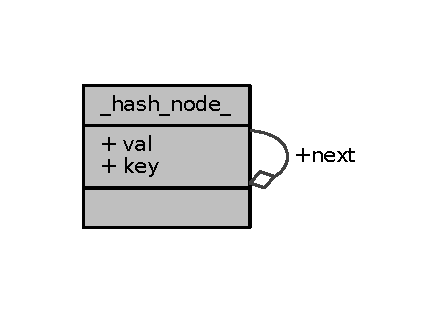
\includegraphics[width=211pt]{struct__hash__node____coll__graph}
\end{center}
\end{figure}
\subsection*{Data Fields}
\begin{DoxyCompactItemize}
\item 
struct \hyperlink{struct__hash__node__}{\-\_\-hash\-\_\-node\-\_\-} $\ast$ \hyperlink{struct__hash__node___a5805097a777732cd94d182bab6c7feb2}{next}
\item 
void $\ast$ \hyperlink{struct__hash__node___ab03f36f103bdec81305fd301f1f93885}{val}
\item 
unsigned int \hyperlink{struct__hash__node___a668a437ea5e7a51173aee9f82f6747de}{key}
\end{DoxyCompactItemize}


\subsection{Field Documentation}
\hypertarget{struct__hash__node___a668a437ea5e7a51173aee9f82f6747de}{\index{\-\_\-hash\-\_\-node\-\_\-@{\-\_\-hash\-\_\-node\-\_\-}!key@{key}}
\index{key@{key}!_hash_node_@{\-\_\-hash\-\_\-node\-\_\-}}
\subsubsection[{key}]{\setlength{\rightskip}{0pt plus 5cm}unsigned int key}}\label{struct__hash__node___a668a437ea5e7a51173aee9f82f6747de}
\hypertarget{struct__hash__node___a5805097a777732cd94d182bab6c7feb2}{\index{\-\_\-hash\-\_\-node\-\_\-@{\-\_\-hash\-\_\-node\-\_\-}!next@{next}}
\index{next@{next}!_hash_node_@{\-\_\-hash\-\_\-node\-\_\-}}
\subsubsection[{next}]{\setlength{\rightskip}{0pt plus 5cm}struct {\bf \-\_\-hash\-\_\-node\-\_\-}$\ast$ next}}\label{struct__hash__node___a5805097a777732cd94d182bab6c7feb2}
\hypertarget{struct__hash__node___ab03f36f103bdec81305fd301f1f93885}{\index{\-\_\-hash\-\_\-node\-\_\-@{\-\_\-hash\-\_\-node\-\_\-}!val@{val}}
\index{val@{val}!_hash_node_@{\-\_\-hash\-\_\-node\-\_\-}}
\subsubsection[{val}]{\setlength{\rightskip}{0pt plus 5cm}void$\ast$ val}}\label{struct__hash__node___ab03f36f103bdec81305fd301f1f93885}


The documentation for this struct was generated from the following file\-:\begin{DoxyCompactItemize}
\item 
inc/\hyperlink{common_8h}{common.\-h}\end{DoxyCompactItemize}

\hypertarget{struct__ipv4__fragment__}{\section{\-\_\-ipv4\-\_\-fragment\-\_\- Struct Reference}
\label{struct__ipv4__fragment__}\index{\-\_\-ipv4\-\_\-fragment\-\_\-@{\-\_\-ipv4\-\_\-fragment\-\_\-}}
}


Struct to store the information of each fragment.  




{\ttfamily \#include $<$ipv4defrag.\-h$>$}



Collaboration diagram for \-\_\-ipv4\-\_\-fragment\-\_\-\-:
\nopagebreak
\begin{figure}[H]
\begin{center}
\leavevmode
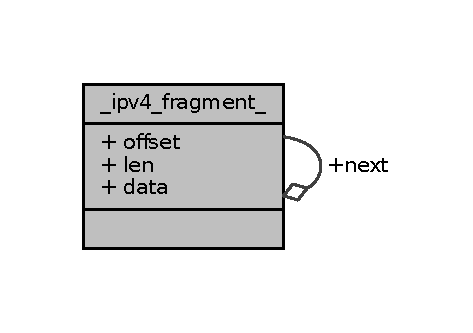
\includegraphics[width=227pt]{struct__ipv4__fragment____coll__graph}
\end{center}
\end{figure}
\subsection*{Data Fields}
\begin{DoxyCompactItemize}
\item 
struct \hyperlink{struct__ipv4__fragment__}{\-\_\-ipv4\-\_\-fragment\-\_\-} $\ast$ \hyperlink{struct__ipv4__fragment___a909d1ac6593a89af1237e515062678a9}{next}
\begin{DoxyCompactList}\small\item\em pointer to the next fragment \end{DoxyCompactList}\item 
unsigned int \hyperlink{struct__ipv4__fragment___a29b5297d3393519050e3126c4cb07c1c}{offset}
\begin{DoxyCompactList}\small\item\em fragment offset \end{DoxyCompactList}\item 
unsigned int \hyperlink{struct__ipv4__fragment___a77124bd5f7e31e6fffc19f335da0c23f}{len}
\begin{DoxyCompactList}\small\item\em fragment data length \end{DoxyCompactList}\item 
unsigned char $\ast$ \hyperlink{struct__ipv4__fragment___ac24cea2bfcc927fd29bc74d1086707d8}{data}
\begin{DoxyCompactList}\small\item\em fragment data \end{DoxyCompactList}\end{DoxyCompactItemize}


\subsection{Detailed Description}
Struct to store the information of each fragment. 

\subsection{Field Documentation}
\hypertarget{struct__ipv4__fragment___ac24cea2bfcc927fd29bc74d1086707d8}{\index{\-\_\-ipv4\-\_\-fragment\-\_\-@{\-\_\-ipv4\-\_\-fragment\-\_\-}!data@{data}}
\index{data@{data}!_ipv4_fragment_@{\-\_\-ipv4\-\_\-fragment\-\_\-}}
\subsubsection[{data}]{\setlength{\rightskip}{0pt plus 5cm}unsigned char$\ast$ data}}\label{struct__ipv4__fragment___ac24cea2bfcc927fd29bc74d1086707d8}


fragment data 

\hypertarget{struct__ipv4__fragment___a77124bd5f7e31e6fffc19f335da0c23f}{\index{\-\_\-ipv4\-\_\-fragment\-\_\-@{\-\_\-ipv4\-\_\-fragment\-\_\-}!len@{len}}
\index{len@{len}!_ipv4_fragment_@{\-\_\-ipv4\-\_\-fragment\-\_\-}}
\subsubsection[{len}]{\setlength{\rightskip}{0pt plus 5cm}unsigned int len}}\label{struct__ipv4__fragment___a77124bd5f7e31e6fffc19f335da0c23f}


fragment data length 

\hypertarget{struct__ipv4__fragment___a909d1ac6593a89af1237e515062678a9}{\index{\-\_\-ipv4\-\_\-fragment\-\_\-@{\-\_\-ipv4\-\_\-fragment\-\_\-}!next@{next}}
\index{next@{next}!_ipv4_fragment_@{\-\_\-ipv4\-\_\-fragment\-\_\-}}
\subsubsection[{next}]{\setlength{\rightskip}{0pt plus 5cm}struct {\bf \-\_\-ipv4\-\_\-fragment\-\_\-}$\ast$ next}}\label{struct__ipv4__fragment___a909d1ac6593a89af1237e515062678a9}


pointer to the next fragment 

\hypertarget{struct__ipv4__fragment___a29b5297d3393519050e3126c4cb07c1c}{\index{\-\_\-ipv4\-\_\-fragment\-\_\-@{\-\_\-ipv4\-\_\-fragment\-\_\-}!offset@{offset}}
\index{offset@{offset}!_ipv4_fragment_@{\-\_\-ipv4\-\_\-fragment\-\_\-}}
\subsubsection[{offset}]{\setlength{\rightskip}{0pt plus 5cm}unsigned int offset}}\label{struct__ipv4__fragment___a29b5297d3393519050e3126c4cb07c1c}


fragment offset 



The documentation for this struct was generated from the following file\-:\begin{DoxyCompactItemize}
\item 
inc/\hyperlink{ipv4defrag_8h}{ipv4defrag.\-h}\end{DoxyCompactItemize}

\hypertarget{struct__ipv4__session__}{\section{\-\_\-ipv4\-\_\-session\-\_\- Struct Reference}
\label{struct__ipv4__session__}\index{\-\_\-ipv4\-\_\-session\-\_\-@{\-\_\-ipv4\-\_\-session\-\_\-}}
}


Structure to store global parameters.  




{\ttfamily \#include $<$ipv4defrag.\-h$>$}



Collaboration diagram for \-\_\-ipv4\-\_\-session\-\_\-\-:
\nopagebreak
\begin{figure}[H]
\begin{center}
\leavevmode
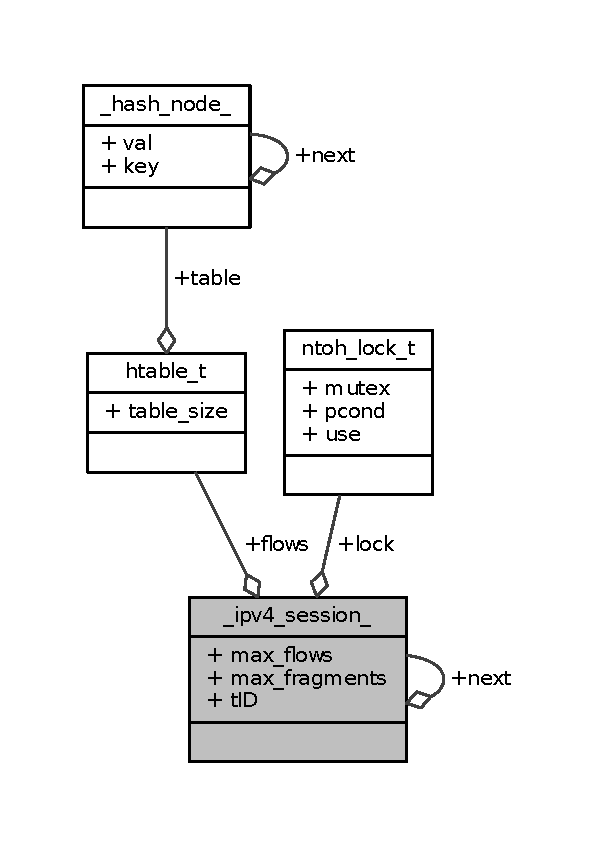
\includegraphics[width=286pt]{struct__ipv4__session____coll__graph}
\end{center}
\end{figure}
\subsection*{Data Fields}
\begin{DoxyCompactItemize}
\item 
struct \hyperlink{struct__ipv4__session__}{\-\_\-ipv4\-\_\-session\-\_\-} $\ast$ \hyperlink{struct__ipv4__session___ad26a99e8003a094ea95493f8b3a22bea}{next}
\item 
sem\-\_\-t \hyperlink{struct__ipv4__session___aba31d11fb16b2f989c42f6433365649e}{max\-\_\-flows}
\begin{DoxyCompactList}\small\item\em max. number of I\-P flows \end{DoxyCompactList}\item 
sem\-\_\-t \hyperlink{struct__ipv4__session___a122dd84b8082b78785803252948a6ad0}{max\-\_\-fragments}
\item 
\hyperlink{ipv4defrag_8h_a7717152886e2f9d1d86e4f28306a5140}{pipv4\-\_\-flows\-\_\-table\-\_\-t} \hyperlink{struct__ipv4__session___ac6eb96500101a7e5b82c6cbdd6e4d12c}{flows}
\begin{DoxyCompactList}\small\item\em hash table to store I\-P flows \end{DoxyCompactList}\item 
pthread\-\_\-t \hyperlink{struct__ipv4__session___ab10186c154259d2b4ed2d25b7e23ed17}{t\-I\-D}
\begin{DoxyCompactList}\small\item\em connection tables related \end{DoxyCompactList}\item 
\hyperlink{structntoh__lock__t}{ntoh\-\_\-lock\-\_\-t} \hyperlink{struct__ipv4__session___aad15823e4f2835531e6a02321cd53f7e}{lock}
\end{DoxyCompactItemize}


\subsection{Detailed Description}
Structure to store global parameters. 

\subsection{Field Documentation}
\hypertarget{struct__ipv4__session___ac6eb96500101a7e5b82c6cbdd6e4d12c}{\index{\-\_\-ipv4\-\_\-session\-\_\-@{\-\_\-ipv4\-\_\-session\-\_\-}!flows@{flows}}
\index{flows@{flows}!_ipv4_session_@{\-\_\-ipv4\-\_\-session\-\_\-}}
\subsubsection[{flows}]{\setlength{\rightskip}{0pt plus 5cm}{\bf pipv4\-\_\-flows\-\_\-table\-\_\-t} flows}}\label{struct__ipv4__session___ac6eb96500101a7e5b82c6cbdd6e4d12c}


hash table to store I\-P flows 

\hypertarget{struct__ipv4__session___aad15823e4f2835531e6a02321cd53f7e}{\index{\-\_\-ipv4\-\_\-session\-\_\-@{\-\_\-ipv4\-\_\-session\-\_\-}!lock@{lock}}
\index{lock@{lock}!_ipv4_session_@{\-\_\-ipv4\-\_\-session\-\_\-}}
\subsubsection[{lock}]{\setlength{\rightskip}{0pt plus 5cm}{\bf ntoh\-\_\-lock\-\_\-t} lock}}\label{struct__ipv4__session___aad15823e4f2835531e6a02321cd53f7e}
\hypertarget{struct__ipv4__session___aba31d11fb16b2f989c42f6433365649e}{\index{\-\_\-ipv4\-\_\-session\-\_\-@{\-\_\-ipv4\-\_\-session\-\_\-}!max\-\_\-flows@{max\-\_\-flows}}
\index{max\-\_\-flows@{max\-\_\-flows}!_ipv4_session_@{\-\_\-ipv4\-\_\-session\-\_\-}}
\subsubsection[{max\-\_\-flows}]{\setlength{\rightskip}{0pt plus 5cm}sem\-\_\-t max\-\_\-flows}}\label{struct__ipv4__session___aba31d11fb16b2f989c42f6433365649e}


max. number of I\-P flows 

\hypertarget{struct__ipv4__session___a122dd84b8082b78785803252948a6ad0}{\index{\-\_\-ipv4\-\_\-session\-\_\-@{\-\_\-ipv4\-\_\-session\-\_\-}!max\-\_\-fragments@{max\-\_\-fragments}}
\index{max\-\_\-fragments@{max\-\_\-fragments}!_ipv4_session_@{\-\_\-ipv4\-\_\-session\-\_\-}}
\subsubsection[{max\-\_\-fragments}]{\setlength{\rightskip}{0pt plus 5cm}sem\-\_\-t max\-\_\-fragments}}\label{struct__ipv4__session___a122dd84b8082b78785803252948a6ad0}
\hypertarget{struct__ipv4__session___ad26a99e8003a094ea95493f8b3a22bea}{\index{\-\_\-ipv4\-\_\-session\-\_\-@{\-\_\-ipv4\-\_\-session\-\_\-}!next@{next}}
\index{next@{next}!_ipv4_session_@{\-\_\-ipv4\-\_\-session\-\_\-}}
\subsubsection[{next}]{\setlength{\rightskip}{0pt plus 5cm}struct {\bf \-\_\-ipv4\-\_\-session\-\_\-}$\ast$ next}}\label{struct__ipv4__session___ad26a99e8003a094ea95493f8b3a22bea}
\hypertarget{struct__ipv4__session___ab10186c154259d2b4ed2d25b7e23ed17}{\index{\-\_\-ipv4\-\_\-session\-\_\-@{\-\_\-ipv4\-\_\-session\-\_\-}!t\-I\-D@{t\-I\-D}}
\index{t\-I\-D@{t\-I\-D}!_ipv4_session_@{\-\_\-ipv4\-\_\-session\-\_\-}}
\subsubsection[{t\-I\-D}]{\setlength{\rightskip}{0pt plus 5cm}pthread\-\_\-t t\-I\-D}}\label{struct__ipv4__session___ab10186c154259d2b4ed2d25b7e23ed17}


connection tables related 



The documentation for this struct was generated from the following file\-:\begin{DoxyCompactItemize}
\item 
inc/\hyperlink{ipv4defrag_8h}{ipv4defrag.\-h}\end{DoxyCompactItemize}

\hypertarget{struct__ipv6__fragment__}{\section{\-\_\-ipv6\-\_\-fragment\-\_\- Struct Reference}
\label{struct__ipv6__fragment__}\index{\-\_\-ipv6\-\_\-fragment\-\_\-@{\-\_\-ipv6\-\_\-fragment\-\_\-}}
}


Struct to store the information of each fragment.  




{\ttfamily \#include $<$ipv6defrag.\-h$>$}



Collaboration diagram for \-\_\-ipv6\-\_\-fragment\-\_\-\-:
\nopagebreak
\begin{figure}[H]
\begin{center}
\leavevmode
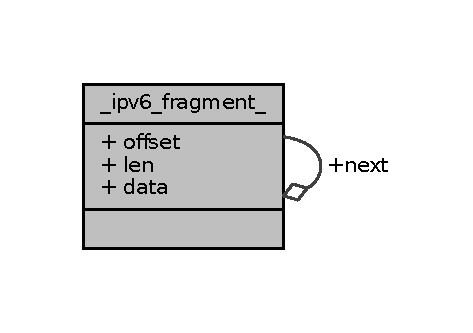
\includegraphics[width=227pt]{struct__ipv6__fragment____coll__graph}
\end{center}
\end{figure}
\subsection*{Data Fields}
\begin{DoxyCompactItemize}
\item 
struct \hyperlink{struct__ipv6__fragment__}{\-\_\-ipv6\-\_\-fragment\-\_\-} $\ast$ \hyperlink{struct__ipv6__fragment___a36d606ad43ccc27ff8dedad831c346b1}{next}
\begin{DoxyCompactList}\small\item\em pointer to the next fragment \end{DoxyCompactList}\item 
unsigned int \hyperlink{struct__ipv6__fragment___a29b5297d3393519050e3126c4cb07c1c}{offset}
\begin{DoxyCompactList}\small\item\em fragment offset \end{DoxyCompactList}\item 
unsigned int \hyperlink{struct__ipv6__fragment___a77124bd5f7e31e6fffc19f335da0c23f}{len}
\begin{DoxyCompactList}\small\item\em fragment data length \end{DoxyCompactList}\item 
unsigned char $\ast$ \hyperlink{struct__ipv6__fragment___ac24cea2bfcc927fd29bc74d1086707d8}{data}
\begin{DoxyCompactList}\small\item\em fragment data \end{DoxyCompactList}\end{DoxyCompactItemize}


\subsection{Detailed Description}
Struct to store the information of each fragment. 

\subsection{Field Documentation}
\hypertarget{struct__ipv6__fragment___ac24cea2bfcc927fd29bc74d1086707d8}{\index{\-\_\-ipv6\-\_\-fragment\-\_\-@{\-\_\-ipv6\-\_\-fragment\-\_\-}!data@{data}}
\index{data@{data}!_ipv6_fragment_@{\-\_\-ipv6\-\_\-fragment\-\_\-}}
\subsubsection[{data}]{\setlength{\rightskip}{0pt plus 5cm}unsigned char$\ast$ data}}\label{struct__ipv6__fragment___ac24cea2bfcc927fd29bc74d1086707d8}


fragment data 

\hypertarget{struct__ipv6__fragment___a77124bd5f7e31e6fffc19f335da0c23f}{\index{\-\_\-ipv6\-\_\-fragment\-\_\-@{\-\_\-ipv6\-\_\-fragment\-\_\-}!len@{len}}
\index{len@{len}!_ipv6_fragment_@{\-\_\-ipv6\-\_\-fragment\-\_\-}}
\subsubsection[{len}]{\setlength{\rightskip}{0pt plus 5cm}unsigned int len}}\label{struct__ipv6__fragment___a77124bd5f7e31e6fffc19f335da0c23f}


fragment data length 

\hypertarget{struct__ipv6__fragment___a36d606ad43ccc27ff8dedad831c346b1}{\index{\-\_\-ipv6\-\_\-fragment\-\_\-@{\-\_\-ipv6\-\_\-fragment\-\_\-}!next@{next}}
\index{next@{next}!_ipv6_fragment_@{\-\_\-ipv6\-\_\-fragment\-\_\-}}
\subsubsection[{next}]{\setlength{\rightskip}{0pt plus 5cm}struct {\bf \-\_\-ipv6\-\_\-fragment\-\_\-}$\ast$ next}}\label{struct__ipv6__fragment___a36d606ad43ccc27ff8dedad831c346b1}


pointer to the next fragment 

\hypertarget{struct__ipv6__fragment___a29b5297d3393519050e3126c4cb07c1c}{\index{\-\_\-ipv6\-\_\-fragment\-\_\-@{\-\_\-ipv6\-\_\-fragment\-\_\-}!offset@{offset}}
\index{offset@{offset}!_ipv6_fragment_@{\-\_\-ipv6\-\_\-fragment\-\_\-}}
\subsubsection[{offset}]{\setlength{\rightskip}{0pt plus 5cm}unsigned int offset}}\label{struct__ipv6__fragment___a29b5297d3393519050e3126c4cb07c1c}


fragment offset 



The documentation for this struct was generated from the following file\-:\begin{DoxyCompactItemize}
\item 
inc/\hyperlink{ipv6defrag_8h}{ipv6defrag.\-h}\end{DoxyCompactItemize}

\hypertarget{struct__ipv6__session__}{\section{\-\_\-ipv6\-\_\-session\-\_\- Struct Reference}
\label{struct__ipv6__session__}\index{\-\_\-ipv6\-\_\-session\-\_\-@{\-\_\-ipv6\-\_\-session\-\_\-}}
}


Structure to store global parameters.  




{\ttfamily \#include $<$ipv6defrag.\-h$>$}



Collaboration diagram for \-\_\-ipv6\-\_\-session\-\_\-\-:
\nopagebreak
\begin{figure}[H]
\begin{center}
\leavevmode
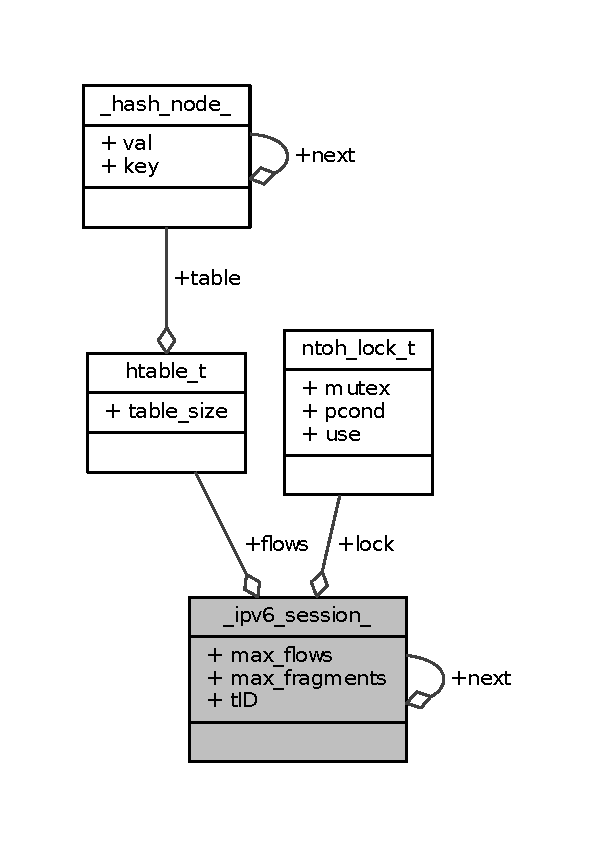
\includegraphics[width=286pt]{struct__ipv6__session____coll__graph}
\end{center}
\end{figure}
\subsection*{Data Fields}
\begin{DoxyCompactItemize}
\item 
struct \hyperlink{struct__ipv6__session__}{\-\_\-ipv6\-\_\-session\-\_\-} $\ast$ \hyperlink{struct__ipv6__session___ac6d0686c91caf00b0b9eaefd9ec5bfcd}{next}
\item 
sem\-\_\-t \hyperlink{struct__ipv6__session___aba31d11fb16b2f989c42f6433365649e}{max\-\_\-flows}
\begin{DoxyCompactList}\small\item\em max. number of I\-P flows \end{DoxyCompactList}\item 
sem\-\_\-t \hyperlink{struct__ipv6__session___a122dd84b8082b78785803252948a6ad0}{max\-\_\-fragments}
\item 
\hyperlink{ipv6defrag_8h_aa864213ee9a224d009da94990b5ba1d7}{pipv6\-\_\-flows\-\_\-table\-\_\-t} \hyperlink{struct__ipv6__session___aecc3227daff3b4522862be5c7d14a9a5}{flows}
\begin{DoxyCompactList}\small\item\em hash table to store I\-P flows \end{DoxyCompactList}\item 
pthread\-\_\-t \hyperlink{struct__ipv6__session___ab10186c154259d2b4ed2d25b7e23ed17}{t\-I\-D}
\begin{DoxyCompactList}\small\item\em connection tables related \end{DoxyCompactList}\item 
\hyperlink{structntoh__lock__t}{ntoh\-\_\-lock\-\_\-t} \hyperlink{struct__ipv6__session___aad15823e4f2835531e6a02321cd53f7e}{lock}
\end{DoxyCompactItemize}


\subsection{Detailed Description}
Structure to store global parameters. 

\subsection{Field Documentation}
\hypertarget{struct__ipv6__session___aecc3227daff3b4522862be5c7d14a9a5}{\index{\-\_\-ipv6\-\_\-session\-\_\-@{\-\_\-ipv6\-\_\-session\-\_\-}!flows@{flows}}
\index{flows@{flows}!_ipv6_session_@{\-\_\-ipv6\-\_\-session\-\_\-}}
\subsubsection[{flows}]{\setlength{\rightskip}{0pt plus 5cm}{\bf pipv6\-\_\-flows\-\_\-table\-\_\-t} flows}}\label{struct__ipv6__session___aecc3227daff3b4522862be5c7d14a9a5}


hash table to store I\-P flows 

\hypertarget{struct__ipv6__session___aad15823e4f2835531e6a02321cd53f7e}{\index{\-\_\-ipv6\-\_\-session\-\_\-@{\-\_\-ipv6\-\_\-session\-\_\-}!lock@{lock}}
\index{lock@{lock}!_ipv6_session_@{\-\_\-ipv6\-\_\-session\-\_\-}}
\subsubsection[{lock}]{\setlength{\rightskip}{0pt plus 5cm}{\bf ntoh\-\_\-lock\-\_\-t} lock}}\label{struct__ipv6__session___aad15823e4f2835531e6a02321cd53f7e}
\hypertarget{struct__ipv6__session___aba31d11fb16b2f989c42f6433365649e}{\index{\-\_\-ipv6\-\_\-session\-\_\-@{\-\_\-ipv6\-\_\-session\-\_\-}!max\-\_\-flows@{max\-\_\-flows}}
\index{max\-\_\-flows@{max\-\_\-flows}!_ipv6_session_@{\-\_\-ipv6\-\_\-session\-\_\-}}
\subsubsection[{max\-\_\-flows}]{\setlength{\rightskip}{0pt plus 5cm}sem\-\_\-t max\-\_\-flows}}\label{struct__ipv6__session___aba31d11fb16b2f989c42f6433365649e}


max. number of I\-P flows 

\hypertarget{struct__ipv6__session___a122dd84b8082b78785803252948a6ad0}{\index{\-\_\-ipv6\-\_\-session\-\_\-@{\-\_\-ipv6\-\_\-session\-\_\-}!max\-\_\-fragments@{max\-\_\-fragments}}
\index{max\-\_\-fragments@{max\-\_\-fragments}!_ipv6_session_@{\-\_\-ipv6\-\_\-session\-\_\-}}
\subsubsection[{max\-\_\-fragments}]{\setlength{\rightskip}{0pt plus 5cm}sem\-\_\-t max\-\_\-fragments}}\label{struct__ipv6__session___a122dd84b8082b78785803252948a6ad0}
\hypertarget{struct__ipv6__session___ac6d0686c91caf00b0b9eaefd9ec5bfcd}{\index{\-\_\-ipv6\-\_\-session\-\_\-@{\-\_\-ipv6\-\_\-session\-\_\-}!next@{next}}
\index{next@{next}!_ipv6_session_@{\-\_\-ipv6\-\_\-session\-\_\-}}
\subsubsection[{next}]{\setlength{\rightskip}{0pt plus 5cm}struct {\bf \-\_\-ipv6\-\_\-session\-\_\-}$\ast$ next}}\label{struct__ipv6__session___ac6d0686c91caf00b0b9eaefd9ec5bfcd}
\hypertarget{struct__ipv6__session___ab10186c154259d2b4ed2d25b7e23ed17}{\index{\-\_\-ipv6\-\_\-session\-\_\-@{\-\_\-ipv6\-\_\-session\-\_\-}!t\-I\-D@{t\-I\-D}}
\index{t\-I\-D@{t\-I\-D}!_ipv6_session_@{\-\_\-ipv6\-\_\-session\-\_\-}}
\subsubsection[{t\-I\-D}]{\setlength{\rightskip}{0pt plus 5cm}pthread\-\_\-t t\-I\-D}}\label{struct__ipv6__session___ab10186c154259d2b4ed2d25b7e23ed17}


connection tables related 



The documentation for this struct was generated from the following file\-:\begin{DoxyCompactItemize}
\item 
inc/\hyperlink{ipv6defrag_8h}{ipv6defrag.\-h}\end{DoxyCompactItemize}

\hypertarget{classlibntoh_1_1__object}{\section{\-\_\-object Class Reference}
\label{classlibntoh_1_1__object}\index{\-\_\-object@{\-\_\-object}}
}


Inheritance diagram for \-\_\-object\-:
\nopagebreak
\begin{figure}[H]
\begin{center}
\leavevmode
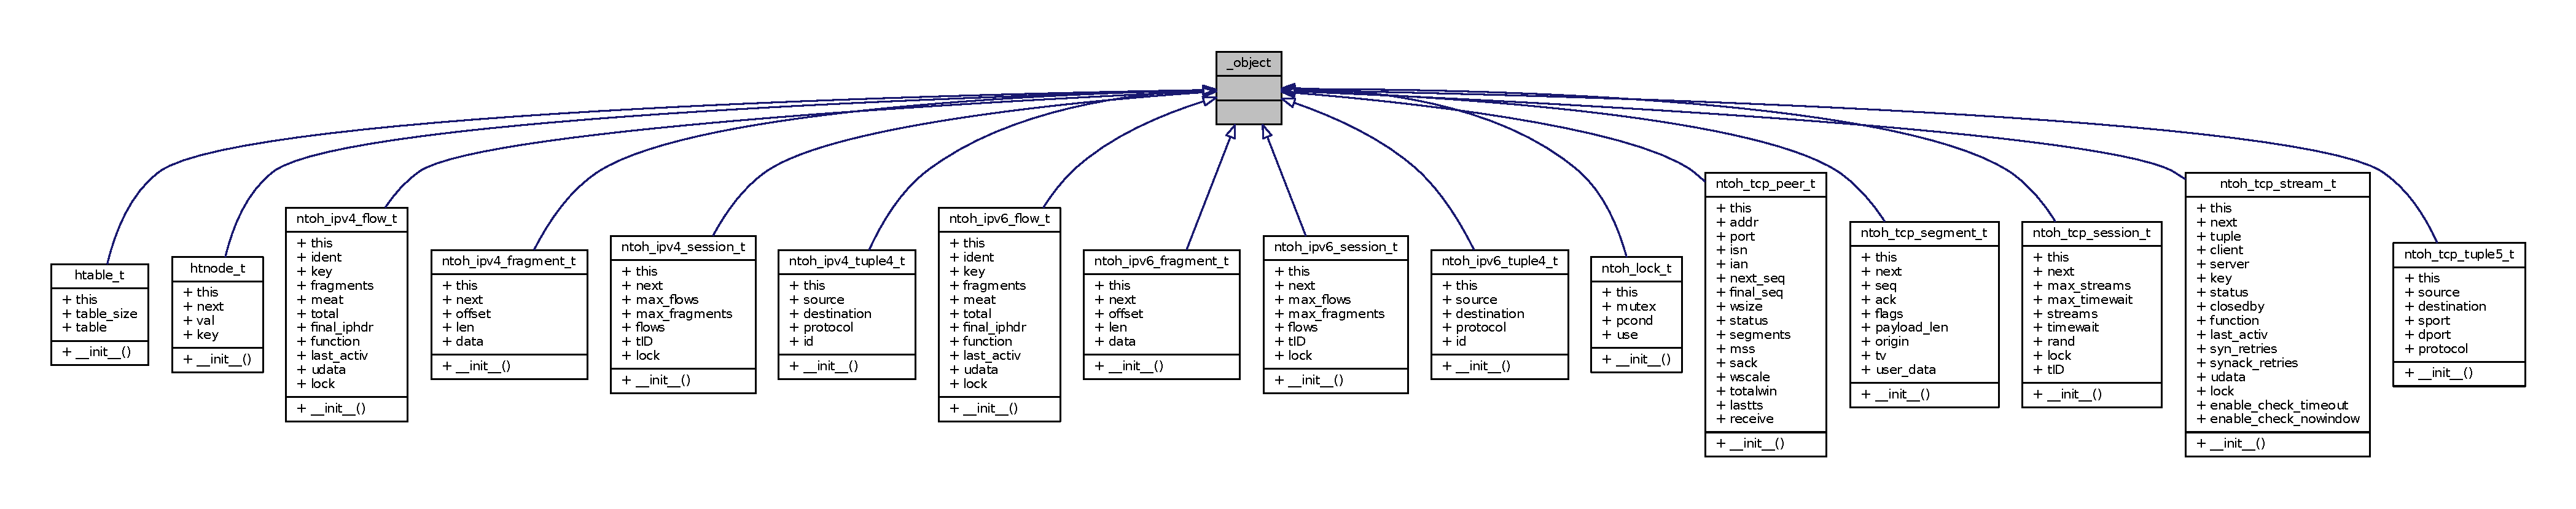
\includegraphics[width=350pt]{classlibntoh_1_1__object__inherit__graph}
\end{center}
\end{figure}


Collaboration diagram for \-\_\-object\-:
\nopagebreak
\begin{figure}[H]
\begin{center}
\leavevmode
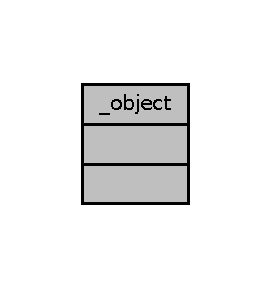
\includegraphics[width=130pt]{classlibntoh_1_1__object__coll__graph}
\end{center}
\end{figure}


The documentation for this class was generated from the following file\-:\begin{DoxyCompactItemize}
\item 
build/\hyperlink{libntoh_8py}{libntoh.\-py}\end{DoxyCompactItemize}

\hypertarget{struct__tcp__segment__}{\section{\-\_\-tcp\-\_\-segment\-\_\- Struct Reference}
\label{struct__tcp__segment__}\index{\-\_\-tcp\-\_\-segment\-\_\-@{\-\_\-tcp\-\_\-segment\-\_\-}}
}


data sent to user-\/function  




{\ttfamily \#include $<$tcpreassembly.\-h$>$}



Collaboration diagram for \-\_\-tcp\-\_\-segment\-\_\-\-:
\nopagebreak
\begin{figure}[H]
\begin{center}
\leavevmode
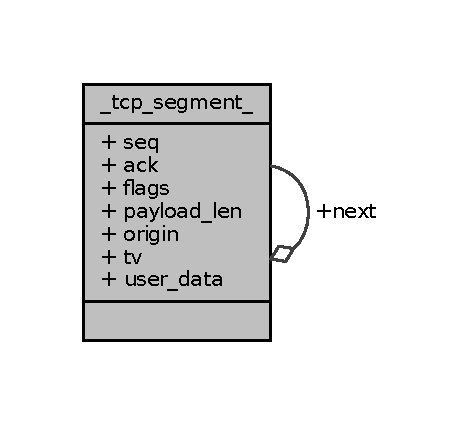
\includegraphics[width=221pt]{struct__tcp__segment____coll__graph}
\end{center}
\end{figure}
\subsection*{Data Fields}
\begin{DoxyCompactItemize}
\item 
struct \hyperlink{struct__tcp__segment__}{\-\_\-tcp\-\_\-segment\-\_\-} $\ast$ \hyperlink{struct__tcp__segment___ae87e4b1042e85d16f28dbf276445d7e9}{next}
\item 
unsigned long \hyperlink{struct__tcp__segment___a189930c4babdc38135a74db479534069}{seq}
\begin{DoxyCompactList}\small\item\em S\-E\-Q number. \end{DoxyCompactList}\item 
unsigned long \hyperlink{struct__tcp__segment___af10658522b9bf1a01d186c69c70efc01}{ack}
\begin{DoxyCompactList}\small\item\em A\-C\-K number. \end{DoxyCompactList}\item 
unsigned char \hyperlink{struct__tcp__segment___a78ac89a4a0f57ffa7c2ecf31749aa390}{flags}
\begin{DoxyCompactList}\small\item\em flags \end{DoxyCompactList}\item 
unsigned int \hyperlink{struct__tcp__segment___a3d431f3cd732945366a2d6d553a69f5c}{payload\-\_\-len}
\begin{DoxyCompactList}\small\item\em payload length \end{DoxyCompactList}\item 
unsigned short \hyperlink{struct__tcp__segment___a2c09a48f3f12ff0e1ed8c7699f52a37d}{origin}
\begin{DoxyCompactList}\small\item\em segment origin \end{DoxyCompactList}\item 
struct timeval \hyperlink{struct__tcp__segment___a9cf96982557d56650f0f4cd3762f05a0}{tv}
\begin{DoxyCompactList}\small\item\em T\-C\-P timestamp. \end{DoxyCompactList}\item 
void $\ast$ \hyperlink{struct__tcp__segment___a0f53d287ac7c064d1a49d4bd93ca1cb9}{user\-\_\-data}
\begin{DoxyCompactList}\small\item\em user provided data \end{DoxyCompactList}\end{DoxyCompactItemize}


\subsection{Detailed Description}
data sent to user-\/function 

\subsection{Field Documentation}
\hypertarget{struct__tcp__segment___af10658522b9bf1a01d186c69c70efc01}{\index{\-\_\-tcp\-\_\-segment\-\_\-@{\-\_\-tcp\-\_\-segment\-\_\-}!ack@{ack}}
\index{ack@{ack}!_tcp_segment_@{\-\_\-tcp\-\_\-segment\-\_\-}}
\subsubsection[{ack}]{\setlength{\rightskip}{0pt plus 5cm}unsigned long ack}}\label{struct__tcp__segment___af10658522b9bf1a01d186c69c70efc01}


A\-C\-K number. 

\hypertarget{struct__tcp__segment___a78ac89a4a0f57ffa7c2ecf31749aa390}{\index{\-\_\-tcp\-\_\-segment\-\_\-@{\-\_\-tcp\-\_\-segment\-\_\-}!flags@{flags}}
\index{flags@{flags}!_tcp_segment_@{\-\_\-tcp\-\_\-segment\-\_\-}}
\subsubsection[{flags}]{\setlength{\rightskip}{0pt plus 5cm}unsigned char flags}}\label{struct__tcp__segment___a78ac89a4a0f57ffa7c2ecf31749aa390}


flags 

\hypertarget{struct__tcp__segment___ae87e4b1042e85d16f28dbf276445d7e9}{\index{\-\_\-tcp\-\_\-segment\-\_\-@{\-\_\-tcp\-\_\-segment\-\_\-}!next@{next}}
\index{next@{next}!_tcp_segment_@{\-\_\-tcp\-\_\-segment\-\_\-}}
\subsubsection[{next}]{\setlength{\rightskip}{0pt plus 5cm}struct {\bf \-\_\-tcp\-\_\-segment\-\_\-}$\ast$ next}}\label{struct__tcp__segment___ae87e4b1042e85d16f28dbf276445d7e9}
\hypertarget{struct__tcp__segment___a2c09a48f3f12ff0e1ed8c7699f52a37d}{\index{\-\_\-tcp\-\_\-segment\-\_\-@{\-\_\-tcp\-\_\-segment\-\_\-}!origin@{origin}}
\index{origin@{origin}!_tcp_segment_@{\-\_\-tcp\-\_\-segment\-\_\-}}
\subsubsection[{origin}]{\setlength{\rightskip}{0pt plus 5cm}unsigned short origin}}\label{struct__tcp__segment___a2c09a48f3f12ff0e1ed8c7699f52a37d}


segment origin 

\hypertarget{struct__tcp__segment___a3d431f3cd732945366a2d6d553a69f5c}{\index{\-\_\-tcp\-\_\-segment\-\_\-@{\-\_\-tcp\-\_\-segment\-\_\-}!payload\-\_\-len@{payload\-\_\-len}}
\index{payload\-\_\-len@{payload\-\_\-len}!_tcp_segment_@{\-\_\-tcp\-\_\-segment\-\_\-}}
\subsubsection[{payload\-\_\-len}]{\setlength{\rightskip}{0pt plus 5cm}unsigned int payload\-\_\-len}}\label{struct__tcp__segment___a3d431f3cd732945366a2d6d553a69f5c}


payload length 

\hypertarget{struct__tcp__segment___a189930c4babdc38135a74db479534069}{\index{\-\_\-tcp\-\_\-segment\-\_\-@{\-\_\-tcp\-\_\-segment\-\_\-}!seq@{seq}}
\index{seq@{seq}!_tcp_segment_@{\-\_\-tcp\-\_\-segment\-\_\-}}
\subsubsection[{seq}]{\setlength{\rightskip}{0pt plus 5cm}unsigned long seq}}\label{struct__tcp__segment___a189930c4babdc38135a74db479534069}


S\-E\-Q number. 

\hypertarget{struct__tcp__segment___a9cf96982557d56650f0f4cd3762f05a0}{\index{\-\_\-tcp\-\_\-segment\-\_\-@{\-\_\-tcp\-\_\-segment\-\_\-}!tv@{tv}}
\index{tv@{tv}!_tcp_segment_@{\-\_\-tcp\-\_\-segment\-\_\-}}
\subsubsection[{tv}]{\setlength{\rightskip}{0pt plus 5cm}struct timeval tv}}\label{struct__tcp__segment___a9cf96982557d56650f0f4cd3762f05a0}


T\-C\-P timestamp. 

\hypertarget{struct__tcp__segment___a0f53d287ac7c064d1a49d4bd93ca1cb9}{\index{\-\_\-tcp\-\_\-segment\-\_\-@{\-\_\-tcp\-\_\-segment\-\_\-}!user\-\_\-data@{user\-\_\-data}}
\index{user\-\_\-data@{user\-\_\-data}!_tcp_segment_@{\-\_\-tcp\-\_\-segment\-\_\-}}
\subsubsection[{user\-\_\-data}]{\setlength{\rightskip}{0pt plus 5cm}void$\ast$ user\-\_\-data}}\label{struct__tcp__segment___a0f53d287ac7c064d1a49d4bd93ca1cb9}


user provided data 



The documentation for this struct was generated from the following file\-:\begin{DoxyCompactItemize}
\item 
inc/\hyperlink{tcpreassembly_8h}{tcpreassembly.\-h}\end{DoxyCompactItemize}

\hypertarget{struct__tcp__session__}{\section{\-\_\-tcp\-\_\-session\-\_\- Struct Reference}
\label{struct__tcp__session__}\index{\-\_\-tcp\-\_\-session\-\_\-@{\-\_\-tcp\-\_\-session\-\_\-}}
}


T\-C\-P session data.  




{\ttfamily \#include $<$tcpreassembly.\-h$>$}



Collaboration diagram for \-\_\-tcp\-\_\-session\-\_\-\-:
\nopagebreak
\begin{figure}[H]
\begin{center}
\leavevmode
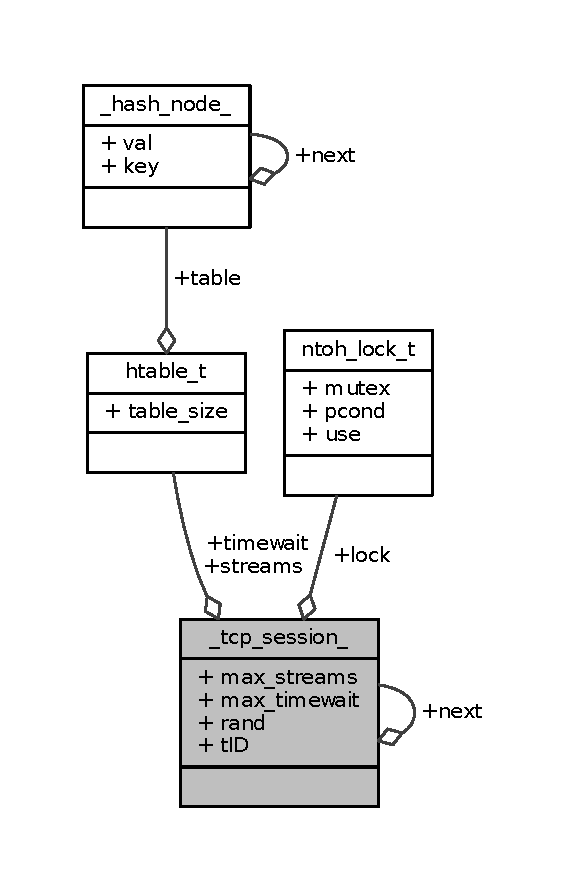
\includegraphics[width=272pt]{struct__tcp__session____coll__graph}
\end{center}
\end{figure}
\subsection*{Data Fields}
\begin{DoxyCompactItemize}
\item 
struct \hyperlink{struct__tcp__session__}{\-\_\-tcp\-\_\-session\-\_\-} $\ast$ \hyperlink{struct__tcp__session___ae866f522c9fbdac668c33af1a598e86f}{next}
\item 
sem\-\_\-t \hyperlink{struct__tcp__session___a8c7b43ddca940d13003768fbd6897aca}{max\-\_\-streams}
\item 
sem\-\_\-t \hyperlink{struct__tcp__session___a0ad4a79087f65efc1af3127c9d9f43a5}{max\-\_\-timewait}
\item 
\hyperlink{tcpreassembly_8h_ae455978c868a3bf1a0708d96932f956a}{ptcprs\-\_\-streams\-\_\-table\-\_\-t} \hyperlink{struct__tcp__session___a5675d32788db8bd40535c108977e8560}{streams}
\item 
\hyperlink{tcpreassembly_8h_ae455978c868a3bf1a0708d96932f956a}{ptcprs\-\_\-streams\-\_\-table\-\_\-t} \hyperlink{struct__tcp__session___a6d12e7905e23f6fd93efd111d40af43c}{timewait}
\item 
int \hyperlink{struct__tcp__session___a19eadb5789a5d63300429365870ec81f}{rand}
\item 
\hyperlink{structntoh__lock__t}{ntoh\-\_\-lock\-\_\-t} \hyperlink{struct__tcp__session___aad15823e4f2835531e6a02321cd53f7e}{lock}
\item 
pthread\-\_\-t \hyperlink{struct__tcp__session___ab10186c154259d2b4ed2d25b7e23ed17}{t\-I\-D}
\end{DoxyCompactItemize}


\subsection{Detailed Description}
T\-C\-P session data. 

\subsection{Field Documentation}
\hypertarget{struct__tcp__session___aad15823e4f2835531e6a02321cd53f7e}{\index{\-\_\-tcp\-\_\-session\-\_\-@{\-\_\-tcp\-\_\-session\-\_\-}!lock@{lock}}
\index{lock@{lock}!_tcp_session_@{\-\_\-tcp\-\_\-session\-\_\-}}
\subsubsection[{lock}]{\setlength{\rightskip}{0pt plus 5cm}{\bf ntoh\-\_\-lock\-\_\-t} lock}}\label{struct__tcp__session___aad15823e4f2835531e6a02321cd53f7e}
\hypertarget{struct__tcp__session___a8c7b43ddca940d13003768fbd6897aca}{\index{\-\_\-tcp\-\_\-session\-\_\-@{\-\_\-tcp\-\_\-session\-\_\-}!max\-\_\-streams@{max\-\_\-streams}}
\index{max\-\_\-streams@{max\-\_\-streams}!_tcp_session_@{\-\_\-tcp\-\_\-session\-\_\-}}
\subsubsection[{max\-\_\-streams}]{\setlength{\rightskip}{0pt plus 5cm}sem\-\_\-t max\-\_\-streams}}\label{struct__tcp__session___a8c7b43ddca940d13003768fbd6897aca}
\hypertarget{struct__tcp__session___a0ad4a79087f65efc1af3127c9d9f43a5}{\index{\-\_\-tcp\-\_\-session\-\_\-@{\-\_\-tcp\-\_\-session\-\_\-}!max\-\_\-timewait@{max\-\_\-timewait}}
\index{max\-\_\-timewait@{max\-\_\-timewait}!_tcp_session_@{\-\_\-tcp\-\_\-session\-\_\-}}
\subsubsection[{max\-\_\-timewait}]{\setlength{\rightskip}{0pt plus 5cm}sem\-\_\-t max\-\_\-timewait}}\label{struct__tcp__session___a0ad4a79087f65efc1af3127c9d9f43a5}
\hypertarget{struct__tcp__session___ae866f522c9fbdac668c33af1a598e86f}{\index{\-\_\-tcp\-\_\-session\-\_\-@{\-\_\-tcp\-\_\-session\-\_\-}!next@{next}}
\index{next@{next}!_tcp_session_@{\-\_\-tcp\-\_\-session\-\_\-}}
\subsubsection[{next}]{\setlength{\rightskip}{0pt plus 5cm}struct {\bf \-\_\-tcp\-\_\-session\-\_\-}$\ast$ next}}\label{struct__tcp__session___ae866f522c9fbdac668c33af1a598e86f}
\hypertarget{struct__tcp__session___a19eadb5789a5d63300429365870ec81f}{\index{\-\_\-tcp\-\_\-session\-\_\-@{\-\_\-tcp\-\_\-session\-\_\-}!rand@{rand}}
\index{rand@{rand}!_tcp_session_@{\-\_\-tcp\-\_\-session\-\_\-}}
\subsubsection[{rand}]{\setlength{\rightskip}{0pt plus 5cm}int rand}}\label{struct__tcp__session___a19eadb5789a5d63300429365870ec81f}
\hypertarget{struct__tcp__session___a5675d32788db8bd40535c108977e8560}{\index{\-\_\-tcp\-\_\-session\-\_\-@{\-\_\-tcp\-\_\-session\-\_\-}!streams@{streams}}
\index{streams@{streams}!_tcp_session_@{\-\_\-tcp\-\_\-session\-\_\-}}
\subsubsection[{streams}]{\setlength{\rightskip}{0pt plus 5cm}{\bf ptcprs\-\_\-streams\-\_\-table\-\_\-t} streams}}\label{struct__tcp__session___a5675d32788db8bd40535c108977e8560}
\hypertarget{struct__tcp__session___ab10186c154259d2b4ed2d25b7e23ed17}{\index{\-\_\-tcp\-\_\-session\-\_\-@{\-\_\-tcp\-\_\-session\-\_\-}!t\-I\-D@{t\-I\-D}}
\index{t\-I\-D@{t\-I\-D}!_tcp_session_@{\-\_\-tcp\-\_\-session\-\_\-}}
\subsubsection[{t\-I\-D}]{\setlength{\rightskip}{0pt plus 5cm}pthread\-\_\-t t\-I\-D}}\label{struct__tcp__session___ab10186c154259d2b4ed2d25b7e23ed17}
\hypertarget{struct__tcp__session___a6d12e7905e23f6fd93efd111d40af43c}{\index{\-\_\-tcp\-\_\-session\-\_\-@{\-\_\-tcp\-\_\-session\-\_\-}!timewait@{timewait}}
\index{timewait@{timewait}!_tcp_session_@{\-\_\-tcp\-\_\-session\-\_\-}}
\subsubsection[{timewait}]{\setlength{\rightskip}{0pt plus 5cm}{\bf ptcprs\-\_\-streams\-\_\-table\-\_\-t} timewait}}\label{struct__tcp__session___a6d12e7905e23f6fd93efd111d40af43c}


The documentation for this struct was generated from the following file\-:\begin{DoxyCompactItemize}
\item 
inc/\hyperlink{tcpreassembly_8h}{tcpreassembly.\-h}\end{DoxyCompactItemize}

\hypertarget{struct__tcp__stream__}{\section{\-\_\-tcp\-\_\-stream\-\_\- Struct Reference}
\label{struct__tcp__stream__}\index{\-\_\-tcp\-\_\-stream\-\_\-@{\-\_\-tcp\-\_\-stream\-\_\-}}
}


connection data  




{\ttfamily \#include $<$tcpreassembly.\-h$>$}



Collaboration diagram for \-\_\-tcp\-\_\-stream\-\_\-\-:
\nopagebreak
\begin{figure}[H]
\begin{center}
\leavevmode
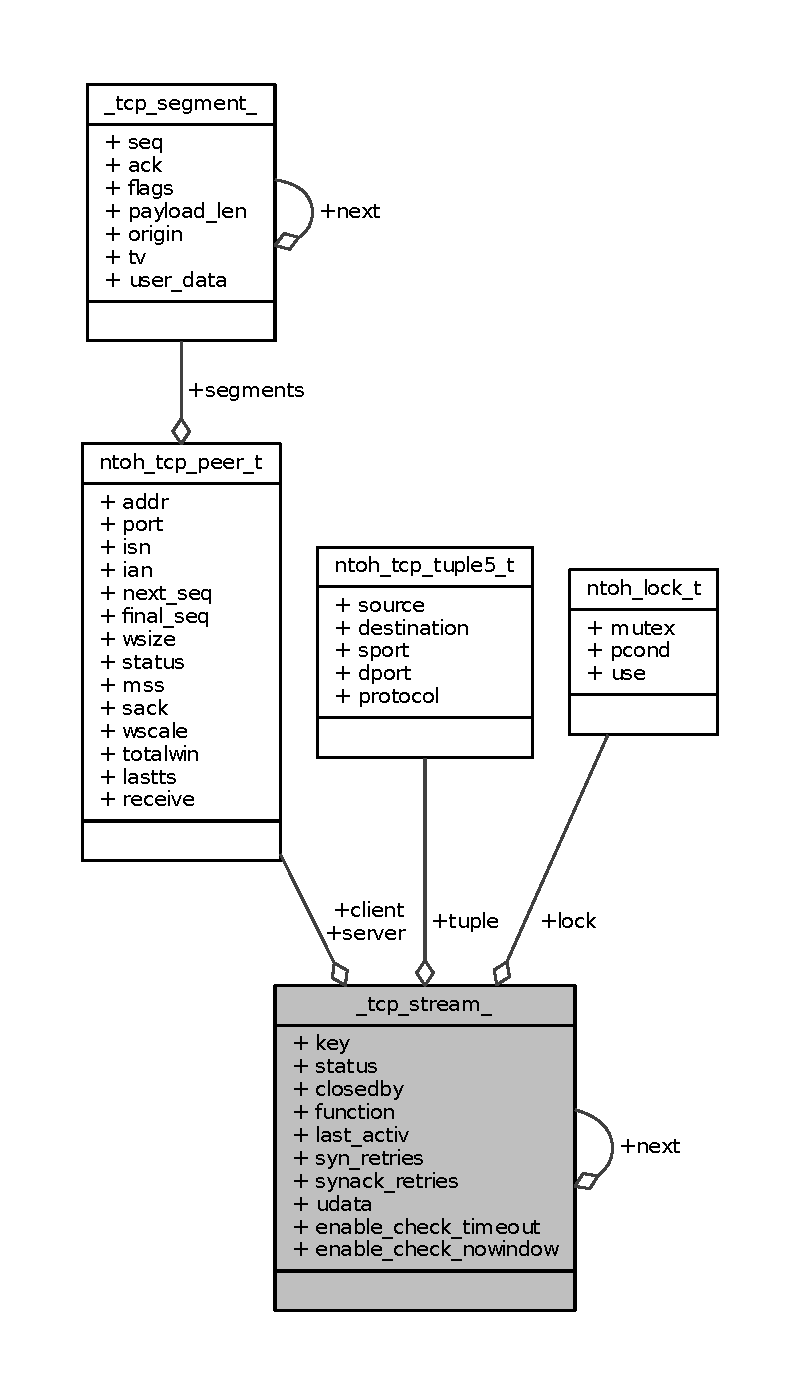
\includegraphics[height=550pt]{struct__tcp__stream____coll__graph}
\end{center}
\end{figure}
\subsection*{Data Fields}
\begin{DoxyCompactItemize}
\item 
struct \hyperlink{struct__tcp__stream__}{\-\_\-tcp\-\_\-stream\-\_\-} $\ast$ \hyperlink{struct__tcp__stream___a7c78f69b0b17c301d5efac15fdf52e8f}{next}
\item 
\hyperlink{structntoh__tcp__tuple5__t}{ntoh\-\_\-tcp\-\_\-tuple5\-\_\-t} \hyperlink{struct__tcp__stream___ace3ecfe5f3174bb45bbead89efe846de}{tuple}
\begin{DoxyCompactList}\small\item\em data to generate the key to identify the connection \end{DoxyCompactList}\item 
\hyperlink{structntoh__tcp__peer__t}{ntoh\-\_\-tcp\-\_\-peer\-\_\-t} \hyperlink{struct__tcp__stream___a1a9f72c5f58a3583f2a54d176e51de0c}{client}
\begin{DoxyCompactList}\small\item\em client data \end{DoxyCompactList}\item 
\hyperlink{structntoh__tcp__peer__t}{ntoh\-\_\-tcp\-\_\-peer\-\_\-t} \hyperlink{struct__tcp__stream___a20b10dfca977ef001517383d7b5e7ad2}{server}
\begin{DoxyCompactList}\small\item\em server data \end{DoxyCompactList}\item 
\hyperlink{tcpreassembly_8h_aa3f9c3d7e8a394f8b2f6329d8f5a8567}{ntoh\-\_\-tcp\-\_\-key\-\_\-t} \hyperlink{struct__tcp__stream___a3e73dbd870716a9514647123a271c681}{key}
\begin{DoxyCompactList}\small\item\em connection key \end{DoxyCompactList}\item 
unsigned int \hyperlink{struct__tcp__stream___aeed08ea57af6f7be240e2bf66162389f}{status}
\begin{DoxyCompactList}\small\item\em connection status \end{DoxyCompactList}\item 
unsigned short \hyperlink{struct__tcp__stream___a6007459c2b9e0960b841fe8fd596b001}{closedby}
\begin{DoxyCompactList}\small\item\em who closed the connection \end{DoxyCompactList}\item 
void $\ast$ \hyperlink{struct__tcp__stream___aea3dcf0c8de30d192ee92494131c4996}{function}
\begin{DoxyCompactList}\small\item\em user-\/defined function to receive data \end{DoxyCompactList}\item 
struct timeval \hyperlink{struct__tcp__stream___a9d115049a50ba4e69eb04c23c973a4a2}{last\-\_\-activ}
\begin{DoxyCompactList}\small\item\em last activity \end{DoxyCompactList}\item 
unsigned int \hyperlink{struct__tcp__stream___ac9513bdb8bd827b1cb22798ae852ba13}{syn\-\_\-retries}
\begin{DoxyCompactList}\small\item\em max. allowed S\-Y\-N retries \end{DoxyCompactList}\item 
unsigned int \hyperlink{struct__tcp__stream___ab971226b37668b378effb81aeba6a63c}{synack\-\_\-retries}
\begin{DoxyCompactList}\small\item\em max. allowed S\-Y\-N/\-A\-C\-K retries \end{DoxyCompactList}\item 
void $\ast$ \hyperlink{struct__tcp__stream___a697ce711b67313990d351b5c95f87aed}{udata}
\begin{DoxyCompactList}\small\item\em user-\/defined data linked to this stream \end{DoxyCompactList}\item 
\hyperlink{structntoh__lock__t}{ntoh\-\_\-lock\-\_\-t} \hyperlink{struct__tcp__stream___aad15823e4f2835531e6a02321cd53f7e}{lock}
\item 
unsigned short \hyperlink{struct__tcp__stream___a23b5d0e5ed45fe6d2771469b246eaa42}{enable\-\_\-check\-\_\-timeout}
\item 
unsigned short \hyperlink{struct__tcp__stream___a5a1f60051aef79a9ac2d6d89ac996da1}{enable\-\_\-check\-\_\-nowindow}
\end{DoxyCompactItemize}


\subsection{Detailed Description}
connection data 

\subsection{Field Documentation}
\hypertarget{struct__tcp__stream___a1a9f72c5f58a3583f2a54d176e51de0c}{\index{\-\_\-tcp\-\_\-stream\-\_\-@{\-\_\-tcp\-\_\-stream\-\_\-}!client@{client}}
\index{client@{client}!_tcp_stream_@{\-\_\-tcp\-\_\-stream\-\_\-}}
\subsubsection[{client}]{\setlength{\rightskip}{0pt plus 5cm}{\bf ntoh\-\_\-tcp\-\_\-peer\-\_\-t} client}}\label{struct__tcp__stream___a1a9f72c5f58a3583f2a54d176e51de0c}


client data 

\hypertarget{struct__tcp__stream___a6007459c2b9e0960b841fe8fd596b001}{\index{\-\_\-tcp\-\_\-stream\-\_\-@{\-\_\-tcp\-\_\-stream\-\_\-}!closedby@{closedby}}
\index{closedby@{closedby}!_tcp_stream_@{\-\_\-tcp\-\_\-stream\-\_\-}}
\subsubsection[{closedby}]{\setlength{\rightskip}{0pt plus 5cm}unsigned short closedby}}\label{struct__tcp__stream___a6007459c2b9e0960b841fe8fd596b001}


who closed the connection 

\hypertarget{struct__tcp__stream___a5a1f60051aef79a9ac2d6d89ac996da1}{\index{\-\_\-tcp\-\_\-stream\-\_\-@{\-\_\-tcp\-\_\-stream\-\_\-}!enable\-\_\-check\-\_\-nowindow@{enable\-\_\-check\-\_\-nowindow}}
\index{enable\-\_\-check\-\_\-nowindow@{enable\-\_\-check\-\_\-nowindow}!_tcp_stream_@{\-\_\-tcp\-\_\-stream\-\_\-}}
\subsubsection[{enable\-\_\-check\-\_\-nowindow}]{\setlength{\rightskip}{0pt plus 5cm}unsigned short enable\-\_\-check\-\_\-nowindow}}\label{struct__tcp__stream___a5a1f60051aef79a9ac2d6d89ac996da1}
\hypertarget{struct__tcp__stream___a23b5d0e5ed45fe6d2771469b246eaa42}{\index{\-\_\-tcp\-\_\-stream\-\_\-@{\-\_\-tcp\-\_\-stream\-\_\-}!enable\-\_\-check\-\_\-timeout@{enable\-\_\-check\-\_\-timeout}}
\index{enable\-\_\-check\-\_\-timeout@{enable\-\_\-check\-\_\-timeout}!_tcp_stream_@{\-\_\-tcp\-\_\-stream\-\_\-}}
\subsubsection[{enable\-\_\-check\-\_\-timeout}]{\setlength{\rightskip}{0pt plus 5cm}unsigned short enable\-\_\-check\-\_\-timeout}}\label{struct__tcp__stream___a23b5d0e5ed45fe6d2771469b246eaa42}
\hypertarget{struct__tcp__stream___aea3dcf0c8de30d192ee92494131c4996}{\index{\-\_\-tcp\-\_\-stream\-\_\-@{\-\_\-tcp\-\_\-stream\-\_\-}!function@{function}}
\index{function@{function}!_tcp_stream_@{\-\_\-tcp\-\_\-stream\-\_\-}}
\subsubsection[{function}]{\setlength{\rightskip}{0pt plus 5cm}void$\ast$ function}}\label{struct__tcp__stream___aea3dcf0c8de30d192ee92494131c4996}


user-\/defined function to receive data 

\hypertarget{struct__tcp__stream___a3e73dbd870716a9514647123a271c681}{\index{\-\_\-tcp\-\_\-stream\-\_\-@{\-\_\-tcp\-\_\-stream\-\_\-}!key@{key}}
\index{key@{key}!_tcp_stream_@{\-\_\-tcp\-\_\-stream\-\_\-}}
\subsubsection[{key}]{\setlength{\rightskip}{0pt plus 5cm}{\bf ntoh\-\_\-tcp\-\_\-key\-\_\-t} key}}\label{struct__tcp__stream___a3e73dbd870716a9514647123a271c681}


connection key 

\hypertarget{struct__tcp__stream___a9d115049a50ba4e69eb04c23c973a4a2}{\index{\-\_\-tcp\-\_\-stream\-\_\-@{\-\_\-tcp\-\_\-stream\-\_\-}!last\-\_\-activ@{last\-\_\-activ}}
\index{last\-\_\-activ@{last\-\_\-activ}!_tcp_stream_@{\-\_\-tcp\-\_\-stream\-\_\-}}
\subsubsection[{last\-\_\-activ}]{\setlength{\rightskip}{0pt plus 5cm}struct timeval last\-\_\-activ}}\label{struct__tcp__stream___a9d115049a50ba4e69eb04c23c973a4a2}


last activity 

\hypertarget{struct__tcp__stream___aad15823e4f2835531e6a02321cd53f7e}{\index{\-\_\-tcp\-\_\-stream\-\_\-@{\-\_\-tcp\-\_\-stream\-\_\-}!lock@{lock}}
\index{lock@{lock}!_tcp_stream_@{\-\_\-tcp\-\_\-stream\-\_\-}}
\subsubsection[{lock}]{\setlength{\rightskip}{0pt plus 5cm}{\bf ntoh\-\_\-lock\-\_\-t} lock}}\label{struct__tcp__stream___aad15823e4f2835531e6a02321cd53f7e}
\hypertarget{struct__tcp__stream___a7c78f69b0b17c301d5efac15fdf52e8f}{\index{\-\_\-tcp\-\_\-stream\-\_\-@{\-\_\-tcp\-\_\-stream\-\_\-}!next@{next}}
\index{next@{next}!_tcp_stream_@{\-\_\-tcp\-\_\-stream\-\_\-}}
\subsubsection[{next}]{\setlength{\rightskip}{0pt plus 5cm}struct {\bf \-\_\-tcp\-\_\-stream\-\_\-}$\ast$ next}}\label{struct__tcp__stream___a7c78f69b0b17c301d5efac15fdf52e8f}
\hypertarget{struct__tcp__stream___a20b10dfca977ef001517383d7b5e7ad2}{\index{\-\_\-tcp\-\_\-stream\-\_\-@{\-\_\-tcp\-\_\-stream\-\_\-}!server@{server}}
\index{server@{server}!_tcp_stream_@{\-\_\-tcp\-\_\-stream\-\_\-}}
\subsubsection[{server}]{\setlength{\rightskip}{0pt plus 5cm}{\bf ntoh\-\_\-tcp\-\_\-peer\-\_\-t} server}}\label{struct__tcp__stream___a20b10dfca977ef001517383d7b5e7ad2}


server data 

\hypertarget{struct__tcp__stream___aeed08ea57af6f7be240e2bf66162389f}{\index{\-\_\-tcp\-\_\-stream\-\_\-@{\-\_\-tcp\-\_\-stream\-\_\-}!status@{status}}
\index{status@{status}!_tcp_stream_@{\-\_\-tcp\-\_\-stream\-\_\-}}
\subsubsection[{status}]{\setlength{\rightskip}{0pt plus 5cm}unsigned int status}}\label{struct__tcp__stream___aeed08ea57af6f7be240e2bf66162389f}


connection status 

\hypertarget{struct__tcp__stream___ac9513bdb8bd827b1cb22798ae852ba13}{\index{\-\_\-tcp\-\_\-stream\-\_\-@{\-\_\-tcp\-\_\-stream\-\_\-}!syn\-\_\-retries@{syn\-\_\-retries}}
\index{syn\-\_\-retries@{syn\-\_\-retries}!_tcp_stream_@{\-\_\-tcp\-\_\-stream\-\_\-}}
\subsubsection[{syn\-\_\-retries}]{\setlength{\rightskip}{0pt plus 5cm}unsigned int syn\-\_\-retries}}\label{struct__tcp__stream___ac9513bdb8bd827b1cb22798ae852ba13}


max. allowed S\-Y\-N retries 

\hypertarget{struct__tcp__stream___ab971226b37668b378effb81aeba6a63c}{\index{\-\_\-tcp\-\_\-stream\-\_\-@{\-\_\-tcp\-\_\-stream\-\_\-}!synack\-\_\-retries@{synack\-\_\-retries}}
\index{synack\-\_\-retries@{synack\-\_\-retries}!_tcp_stream_@{\-\_\-tcp\-\_\-stream\-\_\-}}
\subsubsection[{synack\-\_\-retries}]{\setlength{\rightskip}{0pt plus 5cm}unsigned int synack\-\_\-retries}}\label{struct__tcp__stream___ab971226b37668b378effb81aeba6a63c}


max. allowed S\-Y\-N/\-A\-C\-K retries 

\hypertarget{struct__tcp__stream___ace3ecfe5f3174bb45bbead89efe846de}{\index{\-\_\-tcp\-\_\-stream\-\_\-@{\-\_\-tcp\-\_\-stream\-\_\-}!tuple@{tuple}}
\index{tuple@{tuple}!_tcp_stream_@{\-\_\-tcp\-\_\-stream\-\_\-}}
\subsubsection[{tuple}]{\setlength{\rightskip}{0pt plus 5cm}{\bf ntoh\-\_\-tcp\-\_\-tuple5\-\_\-t} tuple}}\label{struct__tcp__stream___ace3ecfe5f3174bb45bbead89efe846de}


data to generate the key to identify the connection 

\hypertarget{struct__tcp__stream___a697ce711b67313990d351b5c95f87aed}{\index{\-\_\-tcp\-\_\-stream\-\_\-@{\-\_\-tcp\-\_\-stream\-\_\-}!udata@{udata}}
\index{udata@{udata}!_tcp_stream_@{\-\_\-tcp\-\_\-stream\-\_\-}}
\subsubsection[{udata}]{\setlength{\rightskip}{0pt plus 5cm}void$\ast$ udata}}\label{struct__tcp__stream___a697ce711b67313990d351b5c95f87aed}


user-\/defined data linked to this stream 



The documentation for this struct was generated from the following file\-:\begin{DoxyCompactItemize}
\item 
inc/\hyperlink{tcpreassembly_8h}{tcpreassembly.\-h}\end{DoxyCompactItemize}

\hypertarget{classlibntoh_1_1htable__t}{\section{htable\-\_\-t Class Reference}
\label{classlibntoh_1_1htable__t}\index{htable\-\_\-t@{htable\-\_\-t}}
}


Inheritance diagram for htable\-\_\-t\-:
\nopagebreak
\begin{figure}[H]
\begin{center}
\leavevmode
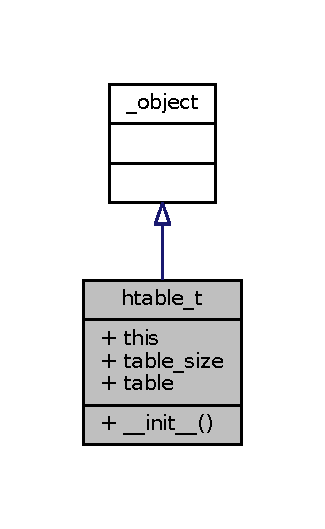
\includegraphics[width=156pt]{classlibntoh_1_1htable__t__inherit__graph}
\end{center}
\end{figure}


Collaboration diagram for htable\-\_\-t\-:
\nopagebreak
\begin{figure}[H]
\begin{center}
\leavevmode
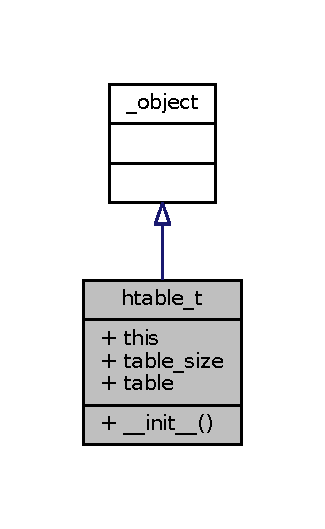
\includegraphics[width=156pt]{classlibntoh_1_1htable__t__coll__graph}
\end{center}
\end{figure}
\subsection*{Public Member Functions}
\begin{DoxyCompactItemize}
\item 
def \hyperlink{classlibntoh_1_1htable__t_ac775ee34451fdfa742b318538164070e}{\-\_\-\-\_\-init\-\_\-\-\_\-}
\end{DoxyCompactItemize}
\subsection*{Data Fields}
\begin{DoxyCompactItemize}
\item 
\hyperlink{classlibntoh_1_1htable__t_a05c09a5e9d53fa7adf0a7936038c2fa3}{this}
\end{DoxyCompactItemize}
\subsection*{Static Public Attributes}
\begin{DoxyCompactItemize}
\item 
tuple \hyperlink{classlibntoh_1_1htable__t_ad67ffd2dbd3d2f980bf246ac3108800d}{table\-\_\-size} = \hyperlink{namespacelibntoh_ae6f5626f776538e0cdb00e75ca1c96c9}{\-\_\-swig\-\_\-property}(\-\_\-libntoh.\-htable\-\_\-t\-\_\-table\-\_\-size\-\_\-get, \-\_\-libntoh.\-htable\-\_\-t\-\_\-table\-\_\-size\-\_\-set)
\item 
tuple \hyperlink{classlibntoh_1_1htable__t_a1d594eec83b20c2174ce4cfea11bdb6b}{table} = \hyperlink{namespacelibntoh_ae6f5626f776538e0cdb00e75ca1c96c9}{\-\_\-swig\-\_\-property}(\-\_\-libntoh.\-htable\-\_\-t\-\_\-table\-\_\-get, \-\_\-libntoh.\-htable\-\_\-t\-\_\-table\-\_\-set)
\end{DoxyCompactItemize}


\subsection{Constructor \& Destructor Documentation}
\hypertarget{classlibntoh_1_1htable__t_ac775ee34451fdfa742b318538164070e}{\index{libntoh\-::htable\-\_\-t@{libntoh\-::htable\-\_\-t}!\-\_\-\-\_\-init\-\_\-\-\_\-@{\-\_\-\-\_\-init\-\_\-\-\_\-}}
\index{\-\_\-\-\_\-init\-\_\-\-\_\-@{\-\_\-\-\_\-init\-\_\-\-\_\-}!libntoh::htable_t@{libntoh\-::htable\-\_\-t}}
\subsubsection[{\-\_\-\-\_\-init\-\_\-\-\_\-}]{\setlength{\rightskip}{0pt plus 5cm}def \-\_\-\-\_\-init\-\_\-\-\_\- (
\begin{DoxyParamCaption}
\item[{}]{self}
\end{DoxyParamCaption}
)}}\label{classlibntoh_1_1htable__t_ac775ee34451fdfa742b318538164070e}


\subsection{Field Documentation}
\hypertarget{classlibntoh_1_1htable__t_a1d594eec83b20c2174ce4cfea11bdb6b}{\index{libntoh\-::htable\-\_\-t@{libntoh\-::htable\-\_\-t}!table@{table}}
\index{table@{table}!libntoh::htable_t@{libntoh\-::htable\-\_\-t}}
\subsubsection[{table}]{\setlength{\rightskip}{0pt plus 5cm}tuple table = {\bf \-\_\-swig\-\_\-property}(\-\_\-libntoh.\-htable\-\_\-t\-\_\-table\-\_\-get, \-\_\-libntoh.\-htable\-\_\-t\-\_\-table\-\_\-set)\hspace{0.3cm}{\ttfamily [static]}}}\label{classlibntoh_1_1htable__t_a1d594eec83b20c2174ce4cfea11bdb6b}
\hypertarget{classlibntoh_1_1htable__t_ad67ffd2dbd3d2f980bf246ac3108800d}{\index{libntoh\-::htable\-\_\-t@{libntoh\-::htable\-\_\-t}!table\-\_\-size@{table\-\_\-size}}
\index{table\-\_\-size@{table\-\_\-size}!libntoh::htable_t@{libntoh\-::htable\-\_\-t}}
\subsubsection[{table\-\_\-size}]{\setlength{\rightskip}{0pt plus 5cm}tuple table\-\_\-size = {\bf \-\_\-swig\-\_\-property}(\-\_\-libntoh.\-htable\-\_\-t\-\_\-table\-\_\-size\-\_\-get, \-\_\-libntoh.\-htable\-\_\-t\-\_\-table\-\_\-size\-\_\-set)\hspace{0.3cm}{\ttfamily [static]}}}\label{classlibntoh_1_1htable__t_ad67ffd2dbd3d2f980bf246ac3108800d}
\hypertarget{classlibntoh_1_1htable__t_a05c09a5e9d53fa7adf0a7936038c2fa3}{\index{libntoh\-::htable\-\_\-t@{libntoh\-::htable\-\_\-t}!this@{this}}
\index{this@{this}!libntoh::htable_t@{libntoh\-::htable\-\_\-t}}
\subsubsection[{this}]{\setlength{\rightskip}{0pt plus 5cm}this}}\label{classlibntoh_1_1htable__t_a05c09a5e9d53fa7adf0a7936038c2fa3}


The documentation for this class was generated from the following file\-:\begin{DoxyCompactItemize}
\item 
build/\hyperlink{libntoh_8py}{libntoh.\-py}\end{DoxyCompactItemize}

\hypertarget{structhtable__t}{\section{htable\-\_\-t Struct Reference}
\label{structhtable__t}\index{htable\-\_\-t@{htable\-\_\-t}}
}


{\ttfamily \#include $<$common.\-h$>$}



Collaboration diagram for htable\-\_\-t\-:
\nopagebreak
\begin{figure}[H]
\begin{center}
\leavevmode
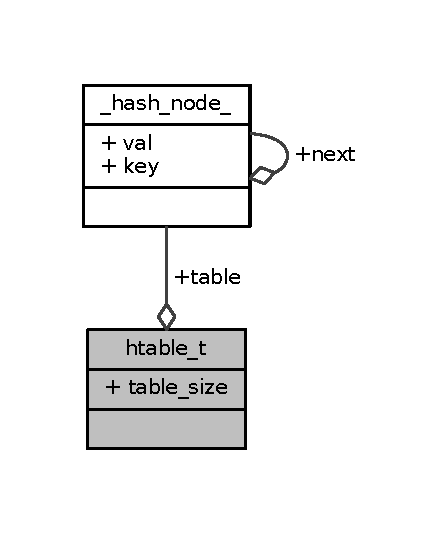
\includegraphics[width=211pt]{structhtable__t__coll__graph}
\end{center}
\end{figure}
\subsection*{Data Fields}
\begin{DoxyCompactItemize}
\item 
size\-\_\-t \hyperlink{structhtable__t_a4b1e1710466cc61c28bae3d4b6e9c063}{table\-\_\-size}
\item 
\hyperlink{common_8h_a083c32a2fd237a02255dbeaa4f72ed4a}{phtnode\-\_\-t} $\ast$ \hyperlink{structhtable__t_a25616ff5782226d344be7754fdb31a79}{table}
\end{DoxyCompactItemize}


\subsection{Field Documentation}
\hypertarget{structhtable__t_a25616ff5782226d344be7754fdb31a79}{\index{htable\-\_\-t@{htable\-\_\-t}!table@{table}}
\index{table@{table}!htable_t@{htable\-\_\-t}}
\subsubsection[{table}]{\setlength{\rightskip}{0pt plus 5cm}{\bf phtnode\-\_\-t}$\ast$ table}}\label{structhtable__t_a25616ff5782226d344be7754fdb31a79}
\hypertarget{structhtable__t_a4b1e1710466cc61c28bae3d4b6e9c063}{\index{htable\-\_\-t@{htable\-\_\-t}!table\-\_\-size@{table\-\_\-size}}
\index{table\-\_\-size@{table\-\_\-size}!htable_t@{htable\-\_\-t}}
\subsubsection[{table\-\_\-size}]{\setlength{\rightskip}{0pt plus 5cm}size\-\_\-t table\-\_\-size}}\label{structhtable__t_a4b1e1710466cc61c28bae3d4b6e9c063}


The documentation for this struct was generated from the following file\-:\begin{DoxyCompactItemize}
\item 
inc/\hyperlink{common_8h}{common.\-h}\end{DoxyCompactItemize}

\hypertarget{classlibntoh_1_1htnode__t}{\section{htnode\-\_\-t Class Reference}
\label{classlibntoh_1_1htnode__t}\index{htnode\-\_\-t@{htnode\-\_\-t}}
}


Inheritance diagram for htnode\-\_\-t\-:
\nopagebreak
\begin{figure}[H]
\begin{center}
\leavevmode
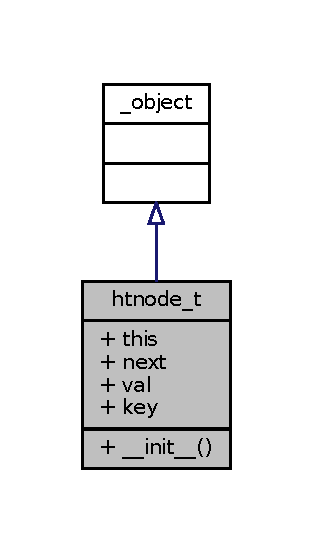
\includegraphics[width=150pt]{classlibntoh_1_1htnode__t__inherit__graph}
\end{center}
\end{figure}


Collaboration diagram for htnode\-\_\-t\-:
\nopagebreak
\begin{figure}[H]
\begin{center}
\leavevmode
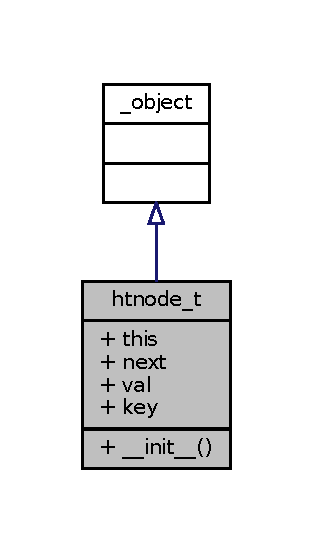
\includegraphics[width=150pt]{classlibntoh_1_1htnode__t__coll__graph}
\end{center}
\end{figure}
\subsection*{Public Member Functions}
\begin{DoxyCompactItemize}
\item 
def \hyperlink{classlibntoh_1_1htnode__t_ac775ee34451fdfa742b318538164070e}{\-\_\-\-\_\-init\-\_\-\-\_\-}
\end{DoxyCompactItemize}
\subsection*{Data Fields}
\begin{DoxyCompactItemize}
\item 
\hyperlink{classlibntoh_1_1htnode__t_a05c09a5e9d53fa7adf0a7936038c2fa3}{this}
\end{DoxyCompactItemize}
\subsection*{Static Public Attributes}
\begin{DoxyCompactItemize}
\item 
tuple \hyperlink{classlibntoh_1_1htnode__t_a84e6dac37062f5a539ece8248c8567cc}{next} = \hyperlink{namespacelibntoh_ae6f5626f776538e0cdb00e75ca1c96c9}{\-\_\-swig\-\_\-property}(\-\_\-libntoh.\-htnode\-\_\-t\-\_\-next\-\_\-get, \-\_\-libntoh.\-htnode\-\_\-t\-\_\-next\-\_\-set)
\item 
tuple \hyperlink{classlibntoh_1_1htnode__t_a8ac4b8dab696ef786dcf547bf611c388}{val} = \hyperlink{namespacelibntoh_ae6f5626f776538e0cdb00e75ca1c96c9}{\-\_\-swig\-\_\-property}(\-\_\-libntoh.\-htnode\-\_\-t\-\_\-val\-\_\-get, \-\_\-libntoh.\-htnode\-\_\-t\-\_\-val\-\_\-set)
\item 
tuple \hyperlink{classlibntoh_1_1htnode__t_a29eb8dd921f77e19e24a20bcd820c2ed}{key} = \hyperlink{namespacelibntoh_ae6f5626f776538e0cdb00e75ca1c96c9}{\-\_\-swig\-\_\-property}(\-\_\-libntoh.\-htnode\-\_\-t\-\_\-key\-\_\-get, \-\_\-libntoh.\-htnode\-\_\-t\-\_\-key\-\_\-set)
\end{DoxyCompactItemize}


\subsection{Constructor \& Destructor Documentation}
\hypertarget{classlibntoh_1_1htnode__t_ac775ee34451fdfa742b318538164070e}{\index{libntoh\-::htnode\-\_\-t@{libntoh\-::htnode\-\_\-t}!\-\_\-\-\_\-init\-\_\-\-\_\-@{\-\_\-\-\_\-init\-\_\-\-\_\-}}
\index{\-\_\-\-\_\-init\-\_\-\-\_\-@{\-\_\-\-\_\-init\-\_\-\-\_\-}!libntoh::htnode_t@{libntoh\-::htnode\-\_\-t}}
\subsubsection[{\-\_\-\-\_\-init\-\_\-\-\_\-}]{\setlength{\rightskip}{0pt plus 5cm}def \-\_\-\-\_\-init\-\_\-\-\_\- (
\begin{DoxyParamCaption}
\item[{}]{self}
\end{DoxyParamCaption}
)}}\label{classlibntoh_1_1htnode__t_ac775ee34451fdfa742b318538164070e}


\subsection{Field Documentation}
\hypertarget{classlibntoh_1_1htnode__t_a29eb8dd921f77e19e24a20bcd820c2ed}{\index{libntoh\-::htnode\-\_\-t@{libntoh\-::htnode\-\_\-t}!key@{key}}
\index{key@{key}!libntoh::htnode_t@{libntoh\-::htnode\-\_\-t}}
\subsubsection[{key}]{\setlength{\rightskip}{0pt plus 5cm}tuple key = {\bf \-\_\-swig\-\_\-property}(\-\_\-libntoh.\-htnode\-\_\-t\-\_\-key\-\_\-get, \-\_\-libntoh.\-htnode\-\_\-t\-\_\-key\-\_\-set)\hspace{0.3cm}{\ttfamily [static]}}}\label{classlibntoh_1_1htnode__t_a29eb8dd921f77e19e24a20bcd820c2ed}
\hypertarget{classlibntoh_1_1htnode__t_a84e6dac37062f5a539ece8248c8567cc}{\index{libntoh\-::htnode\-\_\-t@{libntoh\-::htnode\-\_\-t}!next@{next}}
\index{next@{next}!libntoh::htnode_t@{libntoh\-::htnode\-\_\-t}}
\subsubsection[{next}]{\setlength{\rightskip}{0pt plus 5cm}tuple next = {\bf \-\_\-swig\-\_\-property}(\-\_\-libntoh.\-htnode\-\_\-t\-\_\-next\-\_\-get, \-\_\-libntoh.\-htnode\-\_\-t\-\_\-next\-\_\-set)\hspace{0.3cm}{\ttfamily [static]}}}\label{classlibntoh_1_1htnode__t_a84e6dac37062f5a539ece8248c8567cc}
\hypertarget{classlibntoh_1_1htnode__t_a05c09a5e9d53fa7adf0a7936038c2fa3}{\index{libntoh\-::htnode\-\_\-t@{libntoh\-::htnode\-\_\-t}!this@{this}}
\index{this@{this}!libntoh::htnode_t@{libntoh\-::htnode\-\_\-t}}
\subsubsection[{this}]{\setlength{\rightskip}{0pt plus 5cm}this}}\label{classlibntoh_1_1htnode__t_a05c09a5e9d53fa7adf0a7936038c2fa3}
\hypertarget{classlibntoh_1_1htnode__t_a8ac4b8dab696ef786dcf547bf611c388}{\index{libntoh\-::htnode\-\_\-t@{libntoh\-::htnode\-\_\-t}!val@{val}}
\index{val@{val}!libntoh::htnode_t@{libntoh\-::htnode\-\_\-t}}
\subsubsection[{val}]{\setlength{\rightskip}{0pt plus 5cm}tuple val = {\bf \-\_\-swig\-\_\-property}(\-\_\-libntoh.\-htnode\-\_\-t\-\_\-val\-\_\-get, \-\_\-libntoh.\-htnode\-\_\-t\-\_\-val\-\_\-set)\hspace{0.3cm}{\ttfamily [static]}}}\label{classlibntoh_1_1htnode__t_a8ac4b8dab696ef786dcf547bf611c388}


The documentation for this class was generated from the following file\-:\begin{DoxyCompactItemize}
\item 
build/\hyperlink{libntoh_8py}{libntoh.\-py}\end{DoxyCompactItemize}

\hypertarget{structntoh__ipv4__flow__t}{\section{ntoh\-\_\-ipv4\-\_\-flow\-\_\-t Struct Reference}
\label{structntoh__ipv4__flow__t}\index{ntoh\-\_\-ipv4\-\_\-flow\-\_\-t@{ntoh\-\_\-ipv4\-\_\-flow\-\_\-t}}
}


Struct to store the information of each I\-Pv4 flow.  




{\ttfamily \#include $<$ipv4defrag.\-h$>$}



Collaboration diagram for ntoh\-\_\-ipv4\-\_\-flow\-\_\-t\-:
\nopagebreak
\begin{figure}[H]
\begin{center}
\leavevmode
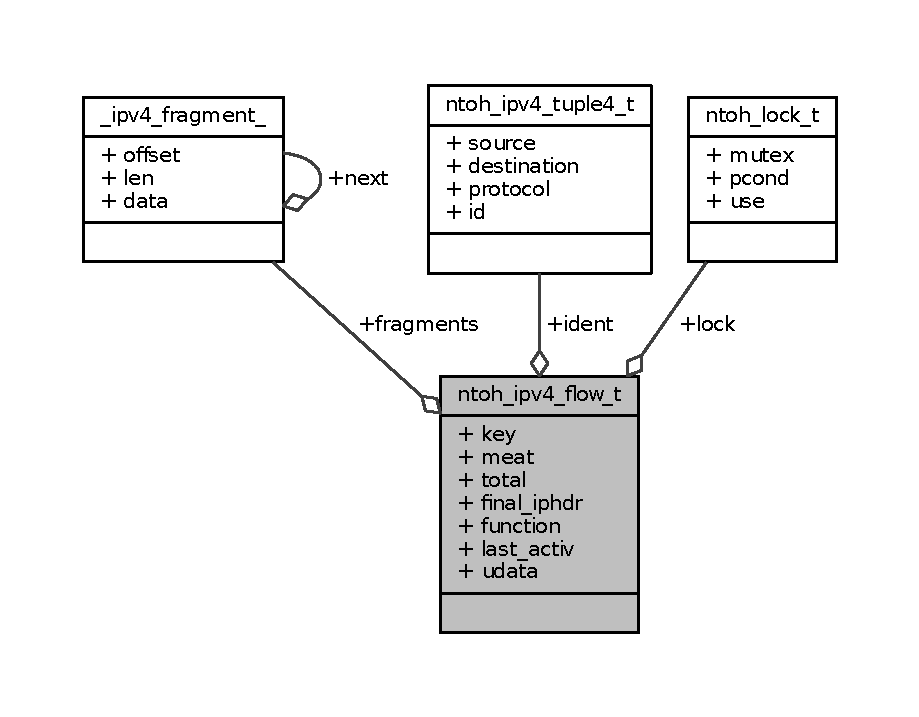
\includegraphics[width=350pt]{structntoh__ipv4__flow__t__coll__graph}
\end{center}
\end{figure}
\subsection*{Data Fields}
\begin{DoxyCompactItemize}
\item 
\hyperlink{structntoh__ipv4__tuple4__t}{ntoh\-\_\-ipv4\-\_\-tuple4\-\_\-t} \hyperlink{structntoh__ipv4__flow__t_a3d4334cd1cad89d0b3401c65411a9cad}{ident}
\begin{DoxyCompactList}\small\item\em flow identification data \end{DoxyCompactList}\item 
\hyperlink{ipv4defrag_8h_ab2ae468c8e84e7b93531ad554b039ca4}{ntoh\-\_\-ipv4\-\_\-key\-\_\-t} \hyperlink{structntoh__ipv4__flow__t_a93bab182dfe815bbd3f8bd00a6a4d4f7}{key}
\begin{DoxyCompactList}\small\item\em flow key \end{DoxyCompactList}\item 
\hyperlink{ipv4defrag_8h_a9b62b0538aa0f37ab5ed16c1d5f24256}{pntoh\-\_\-ipv4\-\_\-fragment\-\_\-t} \hyperlink{structntoh__ipv4__flow__t_a54c94fcc5ec977612392fc7e3bec767f}{fragments}
\begin{DoxyCompactList}\small\item\em fragments list \end{DoxyCompactList}\item 
size\-\_\-t \hyperlink{structntoh__ipv4__flow__t_a25cdc91a1ce3b46649beaacf6315dee7}{meat}
\begin{DoxyCompactList}\small\item\em total amount of received data \end{DoxyCompactList}\item 
size\-\_\-t \hyperlink{structntoh__ipv4__flow__t_a3fab45bb4d7cd7e889bdf00080096e8e}{total}
\begin{DoxyCompactList}\small\item\em total amount of expected data \end{DoxyCompactList}\item 
struct ip $\ast$ \hyperlink{structntoh__ipv4__flow__t_ac53ff70a1958fe8aea9dd55acb1792dd}{final\-\_\-iphdr}
\begin{DoxyCompactList}\small\item\em final fragment received? \end{DoxyCompactList}\item 
void $\ast$ \hyperlink{structntoh__ipv4__flow__t_aea3dcf0c8de30d192ee92494131c4996}{function}
\begin{DoxyCompactList}\small\item\em user defined function to receive defragmented packets \end{DoxyCompactList}\item 
struct timeval \hyperlink{structntoh__ipv4__flow__t_a9d115049a50ba4e69eb04c23c973a4a2}{last\-\_\-activ}
\begin{DoxyCompactList}\small\item\em last activity \end{DoxyCompactList}\item 
void $\ast$ \hyperlink{structntoh__ipv4__flow__t_a697ce711b67313990d351b5c95f87aed}{udata}
\begin{DoxyCompactList}\small\item\em user-\/defined data \end{DoxyCompactList}\item 
\hyperlink{structntoh__lock__t}{ntoh\-\_\-lock\-\_\-t} \hyperlink{structntoh__ipv4__flow__t_aad15823e4f2835531e6a02321cd53f7e}{lock}
\end{DoxyCompactItemize}


\subsection{Detailed Description}
Struct to store the information of each I\-Pv4 flow. 

\subsection{Field Documentation}
\hypertarget{structntoh__ipv4__flow__t_ac53ff70a1958fe8aea9dd55acb1792dd}{\index{ntoh\-\_\-ipv4\-\_\-flow\-\_\-t@{ntoh\-\_\-ipv4\-\_\-flow\-\_\-t}!final\-\_\-iphdr@{final\-\_\-iphdr}}
\index{final\-\_\-iphdr@{final\-\_\-iphdr}!ntoh_ipv4_flow_t@{ntoh\-\_\-ipv4\-\_\-flow\-\_\-t}}
\subsubsection[{final\-\_\-iphdr}]{\setlength{\rightskip}{0pt plus 5cm}struct ip$\ast$ final\-\_\-iphdr}}\label{structntoh__ipv4__flow__t_ac53ff70a1958fe8aea9dd55acb1792dd}


final fragment received? 

\hypertarget{structntoh__ipv4__flow__t_a54c94fcc5ec977612392fc7e3bec767f}{\index{ntoh\-\_\-ipv4\-\_\-flow\-\_\-t@{ntoh\-\_\-ipv4\-\_\-flow\-\_\-t}!fragments@{fragments}}
\index{fragments@{fragments}!ntoh_ipv4_flow_t@{ntoh\-\_\-ipv4\-\_\-flow\-\_\-t}}
\subsubsection[{fragments}]{\setlength{\rightskip}{0pt plus 5cm}{\bf pntoh\-\_\-ipv4\-\_\-fragment\-\_\-t} fragments}}\label{structntoh__ipv4__flow__t_a54c94fcc5ec977612392fc7e3bec767f}


fragments list 

\hypertarget{structntoh__ipv4__flow__t_aea3dcf0c8de30d192ee92494131c4996}{\index{ntoh\-\_\-ipv4\-\_\-flow\-\_\-t@{ntoh\-\_\-ipv4\-\_\-flow\-\_\-t}!function@{function}}
\index{function@{function}!ntoh_ipv4_flow_t@{ntoh\-\_\-ipv4\-\_\-flow\-\_\-t}}
\subsubsection[{function}]{\setlength{\rightskip}{0pt plus 5cm}void$\ast$ function}}\label{structntoh__ipv4__flow__t_aea3dcf0c8de30d192ee92494131c4996}


user defined function to receive defragmented packets 

\hypertarget{structntoh__ipv4__flow__t_a3d4334cd1cad89d0b3401c65411a9cad}{\index{ntoh\-\_\-ipv4\-\_\-flow\-\_\-t@{ntoh\-\_\-ipv4\-\_\-flow\-\_\-t}!ident@{ident}}
\index{ident@{ident}!ntoh_ipv4_flow_t@{ntoh\-\_\-ipv4\-\_\-flow\-\_\-t}}
\subsubsection[{ident}]{\setlength{\rightskip}{0pt plus 5cm}{\bf ntoh\-\_\-ipv4\-\_\-tuple4\-\_\-t} ident}}\label{structntoh__ipv4__flow__t_a3d4334cd1cad89d0b3401c65411a9cad}


flow identification data 

\hypertarget{structntoh__ipv4__flow__t_a93bab182dfe815bbd3f8bd00a6a4d4f7}{\index{ntoh\-\_\-ipv4\-\_\-flow\-\_\-t@{ntoh\-\_\-ipv4\-\_\-flow\-\_\-t}!key@{key}}
\index{key@{key}!ntoh_ipv4_flow_t@{ntoh\-\_\-ipv4\-\_\-flow\-\_\-t}}
\subsubsection[{key}]{\setlength{\rightskip}{0pt plus 5cm}{\bf ntoh\-\_\-ipv4\-\_\-key\-\_\-t} key}}\label{structntoh__ipv4__flow__t_a93bab182dfe815bbd3f8bd00a6a4d4f7}


flow key 

\hypertarget{structntoh__ipv4__flow__t_a9d115049a50ba4e69eb04c23c973a4a2}{\index{ntoh\-\_\-ipv4\-\_\-flow\-\_\-t@{ntoh\-\_\-ipv4\-\_\-flow\-\_\-t}!last\-\_\-activ@{last\-\_\-activ}}
\index{last\-\_\-activ@{last\-\_\-activ}!ntoh_ipv4_flow_t@{ntoh\-\_\-ipv4\-\_\-flow\-\_\-t}}
\subsubsection[{last\-\_\-activ}]{\setlength{\rightskip}{0pt plus 5cm}struct timeval last\-\_\-activ}}\label{structntoh__ipv4__flow__t_a9d115049a50ba4e69eb04c23c973a4a2}


last activity 

\hypertarget{structntoh__ipv4__flow__t_aad15823e4f2835531e6a02321cd53f7e}{\index{ntoh\-\_\-ipv4\-\_\-flow\-\_\-t@{ntoh\-\_\-ipv4\-\_\-flow\-\_\-t}!lock@{lock}}
\index{lock@{lock}!ntoh_ipv4_flow_t@{ntoh\-\_\-ipv4\-\_\-flow\-\_\-t}}
\subsubsection[{lock}]{\setlength{\rightskip}{0pt plus 5cm}{\bf ntoh\-\_\-lock\-\_\-t} lock}}\label{structntoh__ipv4__flow__t_aad15823e4f2835531e6a02321cd53f7e}
\hypertarget{structntoh__ipv4__flow__t_a25cdc91a1ce3b46649beaacf6315dee7}{\index{ntoh\-\_\-ipv4\-\_\-flow\-\_\-t@{ntoh\-\_\-ipv4\-\_\-flow\-\_\-t}!meat@{meat}}
\index{meat@{meat}!ntoh_ipv4_flow_t@{ntoh\-\_\-ipv4\-\_\-flow\-\_\-t}}
\subsubsection[{meat}]{\setlength{\rightskip}{0pt plus 5cm}size\-\_\-t meat}}\label{structntoh__ipv4__flow__t_a25cdc91a1ce3b46649beaacf6315dee7}


total amount of received data 

\hypertarget{structntoh__ipv4__flow__t_a3fab45bb4d7cd7e889bdf00080096e8e}{\index{ntoh\-\_\-ipv4\-\_\-flow\-\_\-t@{ntoh\-\_\-ipv4\-\_\-flow\-\_\-t}!total@{total}}
\index{total@{total}!ntoh_ipv4_flow_t@{ntoh\-\_\-ipv4\-\_\-flow\-\_\-t}}
\subsubsection[{total}]{\setlength{\rightskip}{0pt plus 5cm}size\-\_\-t total}}\label{structntoh__ipv4__flow__t_a3fab45bb4d7cd7e889bdf00080096e8e}


total amount of expected data 

\hypertarget{structntoh__ipv4__flow__t_a697ce711b67313990d351b5c95f87aed}{\index{ntoh\-\_\-ipv4\-\_\-flow\-\_\-t@{ntoh\-\_\-ipv4\-\_\-flow\-\_\-t}!udata@{udata}}
\index{udata@{udata}!ntoh_ipv4_flow_t@{ntoh\-\_\-ipv4\-\_\-flow\-\_\-t}}
\subsubsection[{udata}]{\setlength{\rightskip}{0pt plus 5cm}void$\ast$ udata}}\label{structntoh__ipv4__flow__t_a697ce711b67313990d351b5c95f87aed}


user-\/defined data 



The documentation for this struct was generated from the following file\-:\begin{DoxyCompactItemize}
\item 
inc/\hyperlink{ipv4defrag_8h}{ipv4defrag.\-h}\end{DoxyCompactItemize}

\hypertarget{classlibntoh_1_1ntoh__ipv4__flow__t}{\section{ntoh\-\_\-ipv4\-\_\-flow\-\_\-t Class Reference}
\label{classlibntoh_1_1ntoh__ipv4__flow__t}\index{ntoh\-\_\-ipv4\-\_\-flow\-\_\-t@{ntoh\-\_\-ipv4\-\_\-flow\-\_\-t}}
}


Inheritance diagram for ntoh\-\_\-ipv4\-\_\-flow\-\_\-t\-:
\nopagebreak
\begin{figure}[H]
\begin{center}
\leavevmode
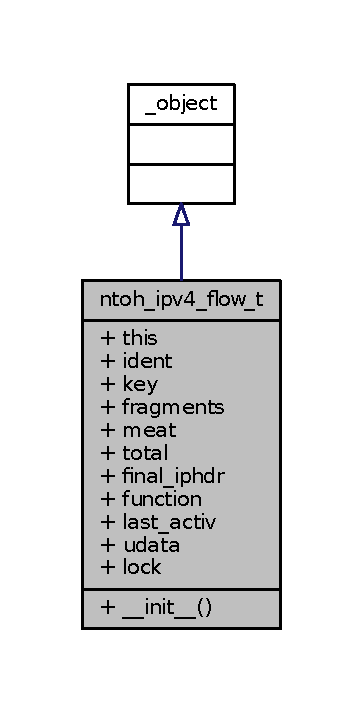
\includegraphics[width=174pt]{classlibntoh_1_1ntoh__ipv4__flow__t__inherit__graph}
\end{center}
\end{figure}


Collaboration diagram for ntoh\-\_\-ipv4\-\_\-flow\-\_\-t\-:
\nopagebreak
\begin{figure}[H]
\begin{center}
\leavevmode
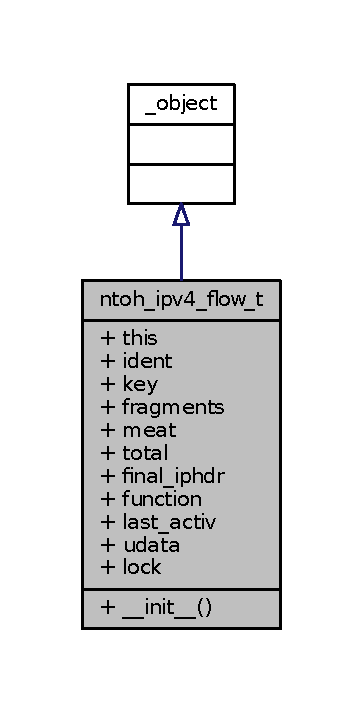
\includegraphics[width=174pt]{classlibntoh_1_1ntoh__ipv4__flow__t__coll__graph}
\end{center}
\end{figure}
\subsection*{Public Member Functions}
\begin{DoxyCompactItemize}
\item 
def \hyperlink{classlibntoh_1_1ntoh__ipv4__flow__t_ac775ee34451fdfa742b318538164070e}{\-\_\-\-\_\-init\-\_\-\-\_\-}
\end{DoxyCompactItemize}
\subsection*{Data Fields}
\begin{DoxyCompactItemize}
\item 
\hyperlink{classlibntoh_1_1ntoh__ipv4__flow__t_a05c09a5e9d53fa7adf0a7936038c2fa3}{this}
\end{DoxyCompactItemize}
\subsection*{Static Public Attributes}
\begin{DoxyCompactItemize}
\item 
tuple \hyperlink{classlibntoh_1_1ntoh__ipv4__flow__t_a219b3ba79a48452030ad36cf2519ee85}{ident} = \hyperlink{namespacelibntoh_ae6f5626f776538e0cdb00e75ca1c96c9}{\-\_\-swig\-\_\-property}(\-\_\-libntoh.\-ntoh\-\_\-ipv4\-\_\-flow\-\_\-t\-\_\-ident\-\_\-get, \-\_\-libntoh.\-ntoh\-\_\-ipv4\-\_\-flow\-\_\-t\-\_\-ident\-\_\-set)
\item 
tuple \hyperlink{classlibntoh_1_1ntoh__ipv4__flow__t_a29eb8dd921f77e19e24a20bcd820c2ed}{key} = \hyperlink{namespacelibntoh_ae6f5626f776538e0cdb00e75ca1c96c9}{\-\_\-swig\-\_\-property}(\-\_\-libntoh.\-ntoh\-\_\-ipv4\-\_\-flow\-\_\-t\-\_\-key\-\_\-get, \-\_\-libntoh.\-ntoh\-\_\-ipv4\-\_\-flow\-\_\-t\-\_\-key\-\_\-set)
\item 
tuple \hyperlink{classlibntoh_1_1ntoh__ipv4__flow__t_a61a562f6a662704721df2bd666792d24}{fragments} = \hyperlink{namespacelibntoh_ae6f5626f776538e0cdb00e75ca1c96c9}{\-\_\-swig\-\_\-property}(\-\_\-libntoh.\-ntoh\-\_\-ipv4\-\_\-flow\-\_\-t\-\_\-fragments\-\_\-get, \-\_\-libntoh.\-ntoh\-\_\-ipv4\-\_\-flow\-\_\-t\-\_\-fragments\-\_\-set)
\item 
tuple \hyperlink{classlibntoh_1_1ntoh__ipv4__flow__t_a05f7a909b2438fcd11159037a9b76457}{meat} = \hyperlink{namespacelibntoh_ae6f5626f776538e0cdb00e75ca1c96c9}{\-\_\-swig\-\_\-property}(\-\_\-libntoh.\-ntoh\-\_\-ipv4\-\_\-flow\-\_\-t\-\_\-meat\-\_\-get, \-\_\-libntoh.\-ntoh\-\_\-ipv4\-\_\-flow\-\_\-t\-\_\-meat\-\_\-set)
\item 
tuple \hyperlink{classlibntoh_1_1ntoh__ipv4__flow__t_a707ba789fae19e34fbeeca4da8c30c5f}{total} = \hyperlink{namespacelibntoh_ae6f5626f776538e0cdb00e75ca1c96c9}{\-\_\-swig\-\_\-property}(\-\_\-libntoh.\-ntoh\-\_\-ipv4\-\_\-flow\-\_\-t\-\_\-total\-\_\-get, \-\_\-libntoh.\-ntoh\-\_\-ipv4\-\_\-flow\-\_\-t\-\_\-total\-\_\-set)
\item 
tuple \hyperlink{classlibntoh_1_1ntoh__ipv4__flow__t_aaae262685d5063d60668907a4beaf956}{final\-\_\-iphdr} = \hyperlink{namespacelibntoh_ae6f5626f776538e0cdb00e75ca1c96c9}{\-\_\-swig\-\_\-property}(\-\_\-libntoh.\-ntoh\-\_\-ipv4\-\_\-flow\-\_\-t\-\_\-final\-\_\-iphdr\-\_\-get, \-\_\-libntoh.\-ntoh\-\_\-ipv4\-\_\-flow\-\_\-t\-\_\-final\-\_\-iphdr\-\_\-set)
\item 
tuple \hyperlink{classlibntoh_1_1ntoh__ipv4__flow__t_a543077174a1281b9d00884a11a040629}{function} = \hyperlink{namespacelibntoh_ae6f5626f776538e0cdb00e75ca1c96c9}{\-\_\-swig\-\_\-property}(\-\_\-libntoh.\-ntoh\-\_\-ipv4\-\_\-flow\-\_\-t\-\_\-function\-\_\-get, \-\_\-libntoh.\-ntoh\-\_\-ipv4\-\_\-flow\-\_\-t\-\_\-function\-\_\-set)
\item 
tuple \hyperlink{classlibntoh_1_1ntoh__ipv4__flow__t_a43a06ba72aed8671dd1579dbf6f78b1a}{last\-\_\-activ} = \hyperlink{namespacelibntoh_ae6f5626f776538e0cdb00e75ca1c96c9}{\-\_\-swig\-\_\-property}(\-\_\-libntoh.\-ntoh\-\_\-ipv4\-\_\-flow\-\_\-t\-\_\-last\-\_\-activ\-\_\-get, \-\_\-libntoh.\-ntoh\-\_\-ipv4\-\_\-flow\-\_\-t\-\_\-last\-\_\-activ\-\_\-set)
\item 
tuple \hyperlink{classlibntoh_1_1ntoh__ipv4__flow__t_a6900744e840ca75a67e020c38d143891}{udata} = \hyperlink{namespacelibntoh_ae6f5626f776538e0cdb00e75ca1c96c9}{\-\_\-swig\-\_\-property}(\-\_\-libntoh.\-ntoh\-\_\-ipv4\-\_\-flow\-\_\-t\-\_\-udata\-\_\-get, \-\_\-libntoh.\-ntoh\-\_\-ipv4\-\_\-flow\-\_\-t\-\_\-udata\-\_\-set)
\item 
tuple \hyperlink{classlibntoh_1_1ntoh__ipv4__flow__t_a871c7bf899334194698c2a3bced5e064}{lock} = \hyperlink{namespacelibntoh_ae6f5626f776538e0cdb00e75ca1c96c9}{\-\_\-swig\-\_\-property}(\-\_\-libntoh.\-ntoh\-\_\-ipv4\-\_\-flow\-\_\-t\-\_\-lock\-\_\-get, \-\_\-libntoh.\-ntoh\-\_\-ipv4\-\_\-flow\-\_\-t\-\_\-lock\-\_\-set)
\end{DoxyCompactItemize}


\subsection{Constructor \& Destructor Documentation}
\hypertarget{classlibntoh_1_1ntoh__ipv4__flow__t_ac775ee34451fdfa742b318538164070e}{\index{libntoh\-::ntoh\-\_\-ipv4\-\_\-flow\-\_\-t@{libntoh\-::ntoh\-\_\-ipv4\-\_\-flow\-\_\-t}!\-\_\-\-\_\-init\-\_\-\-\_\-@{\-\_\-\-\_\-init\-\_\-\-\_\-}}
\index{\-\_\-\-\_\-init\-\_\-\-\_\-@{\-\_\-\-\_\-init\-\_\-\-\_\-}!libntoh::ntoh_ipv4_flow_t@{libntoh\-::ntoh\-\_\-ipv4\-\_\-flow\-\_\-t}}
\subsubsection[{\-\_\-\-\_\-init\-\_\-\-\_\-}]{\setlength{\rightskip}{0pt plus 5cm}def \-\_\-\-\_\-init\-\_\-\-\_\- (
\begin{DoxyParamCaption}
\item[{}]{self}
\end{DoxyParamCaption}
)}}\label{classlibntoh_1_1ntoh__ipv4__flow__t_ac775ee34451fdfa742b318538164070e}


\subsection{Field Documentation}
\hypertarget{classlibntoh_1_1ntoh__ipv4__flow__t_aaae262685d5063d60668907a4beaf956}{\index{libntoh\-::ntoh\-\_\-ipv4\-\_\-flow\-\_\-t@{libntoh\-::ntoh\-\_\-ipv4\-\_\-flow\-\_\-t}!final\-\_\-iphdr@{final\-\_\-iphdr}}
\index{final\-\_\-iphdr@{final\-\_\-iphdr}!libntoh::ntoh_ipv4_flow_t@{libntoh\-::ntoh\-\_\-ipv4\-\_\-flow\-\_\-t}}
\subsubsection[{final\-\_\-iphdr}]{\setlength{\rightskip}{0pt plus 5cm}tuple final\-\_\-iphdr = {\bf \-\_\-swig\-\_\-property}(\-\_\-libntoh.\-ntoh\-\_\-ipv4\-\_\-flow\-\_\-t\-\_\-final\-\_\-iphdr\-\_\-get, \-\_\-libntoh.\-ntoh\-\_\-ipv4\-\_\-flow\-\_\-t\-\_\-final\-\_\-iphdr\-\_\-set)\hspace{0.3cm}{\ttfamily [static]}}}\label{classlibntoh_1_1ntoh__ipv4__flow__t_aaae262685d5063d60668907a4beaf956}
\hypertarget{classlibntoh_1_1ntoh__ipv4__flow__t_a61a562f6a662704721df2bd666792d24}{\index{libntoh\-::ntoh\-\_\-ipv4\-\_\-flow\-\_\-t@{libntoh\-::ntoh\-\_\-ipv4\-\_\-flow\-\_\-t}!fragments@{fragments}}
\index{fragments@{fragments}!libntoh::ntoh_ipv4_flow_t@{libntoh\-::ntoh\-\_\-ipv4\-\_\-flow\-\_\-t}}
\subsubsection[{fragments}]{\setlength{\rightskip}{0pt plus 5cm}tuple fragments = {\bf \-\_\-swig\-\_\-property}(\-\_\-libntoh.\-ntoh\-\_\-ipv4\-\_\-flow\-\_\-t\-\_\-fragments\-\_\-get, \-\_\-libntoh.\-ntoh\-\_\-ipv4\-\_\-flow\-\_\-t\-\_\-fragments\-\_\-set)\hspace{0.3cm}{\ttfamily [static]}}}\label{classlibntoh_1_1ntoh__ipv4__flow__t_a61a562f6a662704721df2bd666792d24}
\hypertarget{classlibntoh_1_1ntoh__ipv4__flow__t_a543077174a1281b9d00884a11a040629}{\index{libntoh\-::ntoh\-\_\-ipv4\-\_\-flow\-\_\-t@{libntoh\-::ntoh\-\_\-ipv4\-\_\-flow\-\_\-t}!function@{function}}
\index{function@{function}!libntoh::ntoh_ipv4_flow_t@{libntoh\-::ntoh\-\_\-ipv4\-\_\-flow\-\_\-t}}
\subsubsection[{function}]{\setlength{\rightskip}{0pt plus 5cm}tuple function = {\bf \-\_\-swig\-\_\-property}(\-\_\-libntoh.\-ntoh\-\_\-ipv4\-\_\-flow\-\_\-t\-\_\-function\-\_\-get, \-\_\-libntoh.\-ntoh\-\_\-ipv4\-\_\-flow\-\_\-t\-\_\-function\-\_\-set)\hspace{0.3cm}{\ttfamily [static]}}}\label{classlibntoh_1_1ntoh__ipv4__flow__t_a543077174a1281b9d00884a11a040629}
\hypertarget{classlibntoh_1_1ntoh__ipv4__flow__t_a219b3ba79a48452030ad36cf2519ee85}{\index{libntoh\-::ntoh\-\_\-ipv4\-\_\-flow\-\_\-t@{libntoh\-::ntoh\-\_\-ipv4\-\_\-flow\-\_\-t}!ident@{ident}}
\index{ident@{ident}!libntoh::ntoh_ipv4_flow_t@{libntoh\-::ntoh\-\_\-ipv4\-\_\-flow\-\_\-t}}
\subsubsection[{ident}]{\setlength{\rightskip}{0pt plus 5cm}tuple ident = {\bf \-\_\-swig\-\_\-property}(\-\_\-libntoh.\-ntoh\-\_\-ipv4\-\_\-flow\-\_\-t\-\_\-ident\-\_\-get, \-\_\-libntoh.\-ntoh\-\_\-ipv4\-\_\-flow\-\_\-t\-\_\-ident\-\_\-set)\hspace{0.3cm}{\ttfamily [static]}}}\label{classlibntoh_1_1ntoh__ipv4__flow__t_a219b3ba79a48452030ad36cf2519ee85}
\hypertarget{classlibntoh_1_1ntoh__ipv4__flow__t_a29eb8dd921f77e19e24a20bcd820c2ed}{\index{libntoh\-::ntoh\-\_\-ipv4\-\_\-flow\-\_\-t@{libntoh\-::ntoh\-\_\-ipv4\-\_\-flow\-\_\-t}!key@{key}}
\index{key@{key}!libntoh::ntoh_ipv4_flow_t@{libntoh\-::ntoh\-\_\-ipv4\-\_\-flow\-\_\-t}}
\subsubsection[{key}]{\setlength{\rightskip}{0pt plus 5cm}tuple key = {\bf \-\_\-swig\-\_\-property}(\-\_\-libntoh.\-ntoh\-\_\-ipv4\-\_\-flow\-\_\-t\-\_\-key\-\_\-get, \-\_\-libntoh.\-ntoh\-\_\-ipv4\-\_\-flow\-\_\-t\-\_\-key\-\_\-set)\hspace{0.3cm}{\ttfamily [static]}}}\label{classlibntoh_1_1ntoh__ipv4__flow__t_a29eb8dd921f77e19e24a20bcd820c2ed}
\hypertarget{classlibntoh_1_1ntoh__ipv4__flow__t_a43a06ba72aed8671dd1579dbf6f78b1a}{\index{libntoh\-::ntoh\-\_\-ipv4\-\_\-flow\-\_\-t@{libntoh\-::ntoh\-\_\-ipv4\-\_\-flow\-\_\-t}!last\-\_\-activ@{last\-\_\-activ}}
\index{last\-\_\-activ@{last\-\_\-activ}!libntoh::ntoh_ipv4_flow_t@{libntoh\-::ntoh\-\_\-ipv4\-\_\-flow\-\_\-t}}
\subsubsection[{last\-\_\-activ}]{\setlength{\rightskip}{0pt plus 5cm}tuple last\-\_\-activ = {\bf \-\_\-swig\-\_\-property}(\-\_\-libntoh.\-ntoh\-\_\-ipv4\-\_\-flow\-\_\-t\-\_\-last\-\_\-activ\-\_\-get, \-\_\-libntoh.\-ntoh\-\_\-ipv4\-\_\-flow\-\_\-t\-\_\-last\-\_\-activ\-\_\-set)\hspace{0.3cm}{\ttfamily [static]}}}\label{classlibntoh_1_1ntoh__ipv4__flow__t_a43a06ba72aed8671dd1579dbf6f78b1a}
\hypertarget{classlibntoh_1_1ntoh__ipv4__flow__t_a871c7bf899334194698c2a3bced5e064}{\index{libntoh\-::ntoh\-\_\-ipv4\-\_\-flow\-\_\-t@{libntoh\-::ntoh\-\_\-ipv4\-\_\-flow\-\_\-t}!lock@{lock}}
\index{lock@{lock}!libntoh::ntoh_ipv4_flow_t@{libntoh\-::ntoh\-\_\-ipv4\-\_\-flow\-\_\-t}}
\subsubsection[{lock}]{\setlength{\rightskip}{0pt plus 5cm}tuple lock = {\bf \-\_\-swig\-\_\-property}(\-\_\-libntoh.\-ntoh\-\_\-ipv4\-\_\-flow\-\_\-t\-\_\-lock\-\_\-get, \-\_\-libntoh.\-ntoh\-\_\-ipv4\-\_\-flow\-\_\-t\-\_\-lock\-\_\-set)\hspace{0.3cm}{\ttfamily [static]}}}\label{classlibntoh_1_1ntoh__ipv4__flow__t_a871c7bf899334194698c2a3bced5e064}
\hypertarget{classlibntoh_1_1ntoh__ipv4__flow__t_a05f7a909b2438fcd11159037a9b76457}{\index{libntoh\-::ntoh\-\_\-ipv4\-\_\-flow\-\_\-t@{libntoh\-::ntoh\-\_\-ipv4\-\_\-flow\-\_\-t}!meat@{meat}}
\index{meat@{meat}!libntoh::ntoh_ipv4_flow_t@{libntoh\-::ntoh\-\_\-ipv4\-\_\-flow\-\_\-t}}
\subsubsection[{meat}]{\setlength{\rightskip}{0pt plus 5cm}tuple meat = {\bf \-\_\-swig\-\_\-property}(\-\_\-libntoh.\-ntoh\-\_\-ipv4\-\_\-flow\-\_\-t\-\_\-meat\-\_\-get, \-\_\-libntoh.\-ntoh\-\_\-ipv4\-\_\-flow\-\_\-t\-\_\-meat\-\_\-set)\hspace{0.3cm}{\ttfamily [static]}}}\label{classlibntoh_1_1ntoh__ipv4__flow__t_a05f7a909b2438fcd11159037a9b76457}
\hypertarget{classlibntoh_1_1ntoh__ipv4__flow__t_a05c09a5e9d53fa7adf0a7936038c2fa3}{\index{libntoh\-::ntoh\-\_\-ipv4\-\_\-flow\-\_\-t@{libntoh\-::ntoh\-\_\-ipv4\-\_\-flow\-\_\-t}!this@{this}}
\index{this@{this}!libntoh::ntoh_ipv4_flow_t@{libntoh\-::ntoh\-\_\-ipv4\-\_\-flow\-\_\-t}}
\subsubsection[{this}]{\setlength{\rightskip}{0pt plus 5cm}this}}\label{classlibntoh_1_1ntoh__ipv4__flow__t_a05c09a5e9d53fa7adf0a7936038c2fa3}
\hypertarget{classlibntoh_1_1ntoh__ipv4__flow__t_a707ba789fae19e34fbeeca4da8c30c5f}{\index{libntoh\-::ntoh\-\_\-ipv4\-\_\-flow\-\_\-t@{libntoh\-::ntoh\-\_\-ipv4\-\_\-flow\-\_\-t}!total@{total}}
\index{total@{total}!libntoh::ntoh_ipv4_flow_t@{libntoh\-::ntoh\-\_\-ipv4\-\_\-flow\-\_\-t}}
\subsubsection[{total}]{\setlength{\rightskip}{0pt plus 5cm}tuple total = {\bf \-\_\-swig\-\_\-property}(\-\_\-libntoh.\-ntoh\-\_\-ipv4\-\_\-flow\-\_\-t\-\_\-total\-\_\-get, \-\_\-libntoh.\-ntoh\-\_\-ipv4\-\_\-flow\-\_\-t\-\_\-total\-\_\-set)\hspace{0.3cm}{\ttfamily [static]}}}\label{classlibntoh_1_1ntoh__ipv4__flow__t_a707ba789fae19e34fbeeca4da8c30c5f}
\hypertarget{classlibntoh_1_1ntoh__ipv4__flow__t_a6900744e840ca75a67e020c38d143891}{\index{libntoh\-::ntoh\-\_\-ipv4\-\_\-flow\-\_\-t@{libntoh\-::ntoh\-\_\-ipv4\-\_\-flow\-\_\-t}!udata@{udata}}
\index{udata@{udata}!libntoh::ntoh_ipv4_flow_t@{libntoh\-::ntoh\-\_\-ipv4\-\_\-flow\-\_\-t}}
\subsubsection[{udata}]{\setlength{\rightskip}{0pt plus 5cm}tuple udata = {\bf \-\_\-swig\-\_\-property}(\-\_\-libntoh.\-ntoh\-\_\-ipv4\-\_\-flow\-\_\-t\-\_\-udata\-\_\-get, \-\_\-libntoh.\-ntoh\-\_\-ipv4\-\_\-flow\-\_\-t\-\_\-udata\-\_\-set)\hspace{0.3cm}{\ttfamily [static]}}}\label{classlibntoh_1_1ntoh__ipv4__flow__t_a6900744e840ca75a67e020c38d143891}


The documentation for this class was generated from the following file\-:\begin{DoxyCompactItemize}
\item 
build/\hyperlink{libntoh_8py}{libntoh.\-py}\end{DoxyCompactItemize}

\hypertarget{classlibntoh_1_1ntoh__ipv4__fragment__t}{\section{ntoh\-\_\-ipv4\-\_\-fragment\-\_\-t Class Reference}
\label{classlibntoh_1_1ntoh__ipv4__fragment__t}\index{ntoh\-\_\-ipv4\-\_\-fragment\-\_\-t@{ntoh\-\_\-ipv4\-\_\-fragment\-\_\-t}}
}


Inheritance diagram for ntoh\-\_\-ipv4\-\_\-fragment\-\_\-t\-:
\nopagebreak
\begin{figure}[H]
\begin{center}
\leavevmode
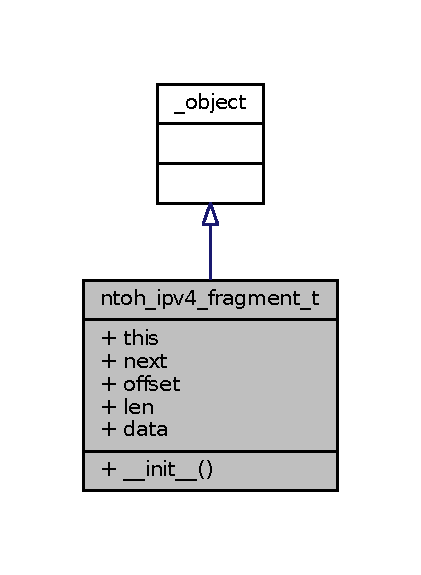
\includegraphics[width=202pt]{classlibntoh_1_1ntoh__ipv4__fragment__t__inherit__graph}
\end{center}
\end{figure}


Collaboration diagram for ntoh\-\_\-ipv4\-\_\-fragment\-\_\-t\-:
\nopagebreak
\begin{figure}[H]
\begin{center}
\leavevmode
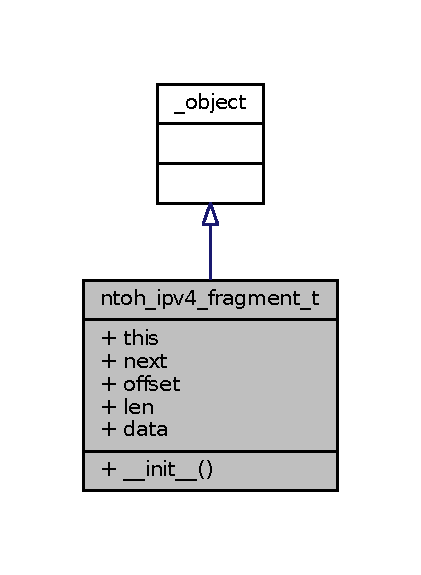
\includegraphics[width=202pt]{classlibntoh_1_1ntoh__ipv4__fragment__t__coll__graph}
\end{center}
\end{figure}
\subsection*{Public Member Functions}
\begin{DoxyCompactItemize}
\item 
def \hyperlink{classlibntoh_1_1ntoh__ipv4__fragment__t_ac775ee34451fdfa742b318538164070e}{\-\_\-\-\_\-init\-\_\-\-\_\-}
\end{DoxyCompactItemize}
\subsection*{Data Fields}
\begin{DoxyCompactItemize}
\item 
\hyperlink{classlibntoh_1_1ntoh__ipv4__fragment__t_a05c09a5e9d53fa7adf0a7936038c2fa3}{this}
\end{DoxyCompactItemize}
\subsection*{Static Public Attributes}
\begin{DoxyCompactItemize}
\item 
tuple \hyperlink{classlibntoh_1_1ntoh__ipv4__fragment__t_a84e6dac37062f5a539ece8248c8567cc}{next} = \hyperlink{namespacelibntoh_ae6f5626f776538e0cdb00e75ca1c96c9}{\-\_\-swig\-\_\-property}(\-\_\-libntoh.\-ntoh\-\_\-ipv4\-\_\-fragment\-\_\-t\-\_\-next\-\_\-get, \-\_\-libntoh.\-ntoh\-\_\-ipv4\-\_\-fragment\-\_\-t\-\_\-next\-\_\-set)
\item 
tuple \hyperlink{classlibntoh_1_1ntoh__ipv4__fragment__t_a03fbaceb13719d1bc975d26c3b92761a}{offset} = \hyperlink{namespacelibntoh_ae6f5626f776538e0cdb00e75ca1c96c9}{\-\_\-swig\-\_\-property}(\-\_\-libntoh.\-ntoh\-\_\-ipv4\-\_\-fragment\-\_\-t\-\_\-offset\-\_\-get, \-\_\-libntoh.\-ntoh\-\_\-ipv4\-\_\-fragment\-\_\-t\-\_\-offset\-\_\-set)
\item 
tuple \hyperlink{classlibntoh_1_1ntoh__ipv4__fragment__t_af8e41b97a0d8adea11037648944de58f}{len} = \hyperlink{namespacelibntoh_ae6f5626f776538e0cdb00e75ca1c96c9}{\-\_\-swig\-\_\-property}(\-\_\-libntoh.\-ntoh\-\_\-ipv4\-\_\-fragment\-\_\-t\-\_\-len\-\_\-get, \-\_\-libntoh.\-ntoh\-\_\-ipv4\-\_\-fragment\-\_\-t\-\_\-len\-\_\-set)
\item 
tuple \hyperlink{classlibntoh_1_1ntoh__ipv4__fragment__t_aa7a0efb8690a34f61a95b00cc723ca27}{data} = \hyperlink{namespacelibntoh_ae6f5626f776538e0cdb00e75ca1c96c9}{\-\_\-swig\-\_\-property}(\-\_\-libntoh.\-ntoh\-\_\-ipv4\-\_\-fragment\-\_\-t\-\_\-data\-\_\-get, \-\_\-libntoh.\-ntoh\-\_\-ipv4\-\_\-fragment\-\_\-t\-\_\-data\-\_\-set)
\end{DoxyCompactItemize}


\subsection{Constructor \& Destructor Documentation}
\hypertarget{classlibntoh_1_1ntoh__ipv4__fragment__t_ac775ee34451fdfa742b318538164070e}{\index{libntoh\-::ntoh\-\_\-ipv4\-\_\-fragment\-\_\-t@{libntoh\-::ntoh\-\_\-ipv4\-\_\-fragment\-\_\-t}!\-\_\-\-\_\-init\-\_\-\-\_\-@{\-\_\-\-\_\-init\-\_\-\-\_\-}}
\index{\-\_\-\-\_\-init\-\_\-\-\_\-@{\-\_\-\-\_\-init\-\_\-\-\_\-}!libntoh::ntoh_ipv4_fragment_t@{libntoh\-::ntoh\-\_\-ipv4\-\_\-fragment\-\_\-t}}
\subsubsection[{\-\_\-\-\_\-init\-\_\-\-\_\-}]{\setlength{\rightskip}{0pt plus 5cm}def \-\_\-\-\_\-init\-\_\-\-\_\- (
\begin{DoxyParamCaption}
\item[{}]{self}
\end{DoxyParamCaption}
)}}\label{classlibntoh_1_1ntoh__ipv4__fragment__t_ac775ee34451fdfa742b318538164070e}


\subsection{Field Documentation}
\hypertarget{classlibntoh_1_1ntoh__ipv4__fragment__t_aa7a0efb8690a34f61a95b00cc723ca27}{\index{libntoh\-::ntoh\-\_\-ipv4\-\_\-fragment\-\_\-t@{libntoh\-::ntoh\-\_\-ipv4\-\_\-fragment\-\_\-t}!data@{data}}
\index{data@{data}!libntoh::ntoh_ipv4_fragment_t@{libntoh\-::ntoh\-\_\-ipv4\-\_\-fragment\-\_\-t}}
\subsubsection[{data}]{\setlength{\rightskip}{0pt plus 5cm}tuple data = {\bf \-\_\-swig\-\_\-property}(\-\_\-libntoh.\-ntoh\-\_\-ipv4\-\_\-fragment\-\_\-t\-\_\-data\-\_\-get, \-\_\-libntoh.\-ntoh\-\_\-ipv4\-\_\-fragment\-\_\-t\-\_\-data\-\_\-set)\hspace{0.3cm}{\ttfamily [static]}}}\label{classlibntoh_1_1ntoh__ipv4__fragment__t_aa7a0efb8690a34f61a95b00cc723ca27}
\hypertarget{classlibntoh_1_1ntoh__ipv4__fragment__t_af8e41b97a0d8adea11037648944de58f}{\index{libntoh\-::ntoh\-\_\-ipv4\-\_\-fragment\-\_\-t@{libntoh\-::ntoh\-\_\-ipv4\-\_\-fragment\-\_\-t}!len@{len}}
\index{len@{len}!libntoh::ntoh_ipv4_fragment_t@{libntoh\-::ntoh\-\_\-ipv4\-\_\-fragment\-\_\-t}}
\subsubsection[{len}]{\setlength{\rightskip}{0pt plus 5cm}tuple len = {\bf \-\_\-swig\-\_\-property}(\-\_\-libntoh.\-ntoh\-\_\-ipv4\-\_\-fragment\-\_\-t\-\_\-len\-\_\-get, \-\_\-libntoh.\-ntoh\-\_\-ipv4\-\_\-fragment\-\_\-t\-\_\-len\-\_\-set)\hspace{0.3cm}{\ttfamily [static]}}}\label{classlibntoh_1_1ntoh__ipv4__fragment__t_af8e41b97a0d8adea11037648944de58f}
\hypertarget{classlibntoh_1_1ntoh__ipv4__fragment__t_a84e6dac37062f5a539ece8248c8567cc}{\index{libntoh\-::ntoh\-\_\-ipv4\-\_\-fragment\-\_\-t@{libntoh\-::ntoh\-\_\-ipv4\-\_\-fragment\-\_\-t}!next@{next}}
\index{next@{next}!libntoh::ntoh_ipv4_fragment_t@{libntoh\-::ntoh\-\_\-ipv4\-\_\-fragment\-\_\-t}}
\subsubsection[{next}]{\setlength{\rightskip}{0pt plus 5cm}tuple next = {\bf \-\_\-swig\-\_\-property}(\-\_\-libntoh.\-ntoh\-\_\-ipv4\-\_\-fragment\-\_\-t\-\_\-next\-\_\-get, \-\_\-libntoh.\-ntoh\-\_\-ipv4\-\_\-fragment\-\_\-t\-\_\-next\-\_\-set)\hspace{0.3cm}{\ttfamily [static]}}}\label{classlibntoh_1_1ntoh__ipv4__fragment__t_a84e6dac37062f5a539ece8248c8567cc}
\hypertarget{classlibntoh_1_1ntoh__ipv4__fragment__t_a03fbaceb13719d1bc975d26c3b92761a}{\index{libntoh\-::ntoh\-\_\-ipv4\-\_\-fragment\-\_\-t@{libntoh\-::ntoh\-\_\-ipv4\-\_\-fragment\-\_\-t}!offset@{offset}}
\index{offset@{offset}!libntoh::ntoh_ipv4_fragment_t@{libntoh\-::ntoh\-\_\-ipv4\-\_\-fragment\-\_\-t}}
\subsubsection[{offset}]{\setlength{\rightskip}{0pt plus 5cm}tuple offset = {\bf \-\_\-swig\-\_\-property}(\-\_\-libntoh.\-ntoh\-\_\-ipv4\-\_\-fragment\-\_\-t\-\_\-offset\-\_\-get, \-\_\-libntoh.\-ntoh\-\_\-ipv4\-\_\-fragment\-\_\-t\-\_\-offset\-\_\-set)\hspace{0.3cm}{\ttfamily [static]}}}\label{classlibntoh_1_1ntoh__ipv4__fragment__t_a03fbaceb13719d1bc975d26c3b92761a}
\hypertarget{classlibntoh_1_1ntoh__ipv4__fragment__t_a05c09a5e9d53fa7adf0a7936038c2fa3}{\index{libntoh\-::ntoh\-\_\-ipv4\-\_\-fragment\-\_\-t@{libntoh\-::ntoh\-\_\-ipv4\-\_\-fragment\-\_\-t}!this@{this}}
\index{this@{this}!libntoh::ntoh_ipv4_fragment_t@{libntoh\-::ntoh\-\_\-ipv4\-\_\-fragment\-\_\-t}}
\subsubsection[{this}]{\setlength{\rightskip}{0pt plus 5cm}this}}\label{classlibntoh_1_1ntoh__ipv4__fragment__t_a05c09a5e9d53fa7adf0a7936038c2fa3}


The documentation for this class was generated from the following file\-:\begin{DoxyCompactItemize}
\item 
build/\hyperlink{libntoh_8py}{libntoh.\-py}\end{DoxyCompactItemize}

\hypertarget{classlibntoh_1_1ntoh__ipv4__session__t}{\section{ntoh\-\_\-ipv4\-\_\-session\-\_\-t Class Reference}
\label{classlibntoh_1_1ntoh__ipv4__session__t}\index{ntoh\-\_\-ipv4\-\_\-session\-\_\-t@{ntoh\-\_\-ipv4\-\_\-session\-\_\-t}}
}


Inheritance diagram for ntoh\-\_\-ipv4\-\_\-session\-\_\-t\-:
\nopagebreak
\begin{figure}[H]
\begin{center}
\leavevmode
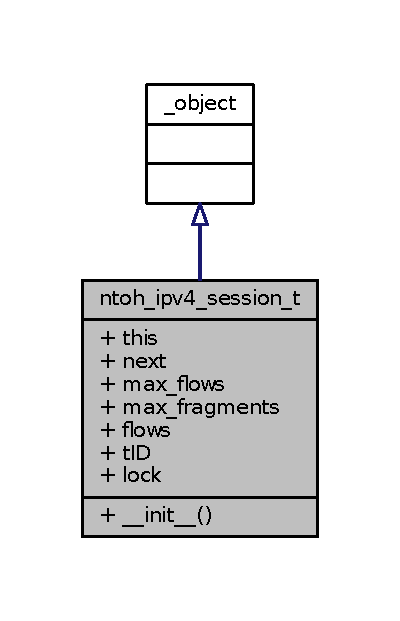
\includegraphics[width=192pt]{classlibntoh_1_1ntoh__ipv4__session__t__inherit__graph}
\end{center}
\end{figure}


Collaboration diagram for ntoh\-\_\-ipv4\-\_\-session\-\_\-t\-:
\nopagebreak
\begin{figure}[H]
\begin{center}
\leavevmode
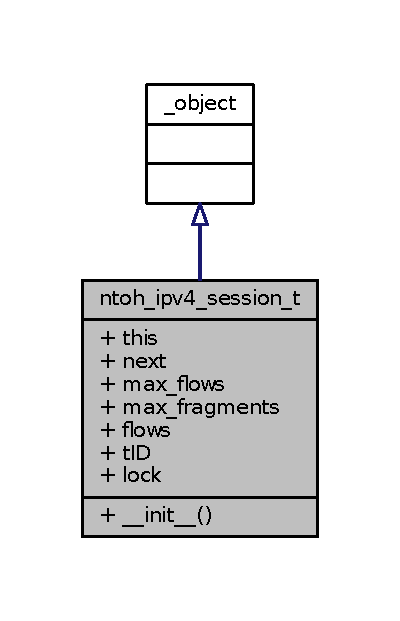
\includegraphics[width=192pt]{classlibntoh_1_1ntoh__ipv4__session__t__coll__graph}
\end{center}
\end{figure}
\subsection*{Public Member Functions}
\begin{DoxyCompactItemize}
\item 
def \hyperlink{classlibntoh_1_1ntoh__ipv4__session__t_ac775ee34451fdfa742b318538164070e}{\-\_\-\-\_\-init\-\_\-\-\_\-}
\end{DoxyCompactItemize}
\subsection*{Data Fields}
\begin{DoxyCompactItemize}
\item 
\hyperlink{classlibntoh_1_1ntoh__ipv4__session__t_a05c09a5e9d53fa7adf0a7936038c2fa3}{this}
\end{DoxyCompactItemize}
\subsection*{Static Public Attributes}
\begin{DoxyCompactItemize}
\item 
tuple \hyperlink{classlibntoh_1_1ntoh__ipv4__session__t_a84e6dac37062f5a539ece8248c8567cc}{next} = \hyperlink{namespacelibntoh_ae6f5626f776538e0cdb00e75ca1c96c9}{\-\_\-swig\-\_\-property}(\-\_\-libntoh.\-ntoh\-\_\-ipv4\-\_\-session\-\_\-t\-\_\-next\-\_\-get, \-\_\-libntoh.\-ntoh\-\_\-ipv4\-\_\-session\-\_\-t\-\_\-next\-\_\-set)
\item 
tuple \hyperlink{classlibntoh_1_1ntoh__ipv4__session__t_af05028fd588ff1bc962a8a89057a3716}{max\-\_\-flows} = \hyperlink{namespacelibntoh_ae6f5626f776538e0cdb00e75ca1c96c9}{\-\_\-swig\-\_\-property}(\-\_\-libntoh.\-ntoh\-\_\-ipv4\-\_\-session\-\_\-t\-\_\-max\-\_\-flows\-\_\-get, \-\_\-libntoh.\-ntoh\-\_\-ipv4\-\_\-session\-\_\-t\-\_\-max\-\_\-flows\-\_\-set)
\item 
tuple \hyperlink{classlibntoh_1_1ntoh__ipv4__session__t_aae26317f4443b9f0f36780fb035d1ec9}{max\-\_\-fragments} = \hyperlink{namespacelibntoh_ae6f5626f776538e0cdb00e75ca1c96c9}{\-\_\-swig\-\_\-property}(\-\_\-libntoh.\-ntoh\-\_\-ipv4\-\_\-session\-\_\-t\-\_\-max\-\_\-fragments\-\_\-get, \-\_\-libntoh.\-ntoh\-\_\-ipv4\-\_\-session\-\_\-t\-\_\-max\-\_\-fragments\-\_\-set)
\item 
tuple \hyperlink{classlibntoh_1_1ntoh__ipv4__session__t_afca3cb4196e6410df799227741f11b5e}{flows} = \hyperlink{namespacelibntoh_ae6f5626f776538e0cdb00e75ca1c96c9}{\-\_\-swig\-\_\-property}(\-\_\-libntoh.\-ntoh\-\_\-ipv4\-\_\-session\-\_\-t\-\_\-flows\-\_\-get, \-\_\-libntoh.\-ntoh\-\_\-ipv4\-\_\-session\-\_\-t\-\_\-flows\-\_\-set)
\item 
tuple \hyperlink{classlibntoh_1_1ntoh__ipv4__session__t_aa8af5c32a2a96a7fe7e14b7ebd2057ba}{t\-I\-D} = \hyperlink{namespacelibntoh_ae6f5626f776538e0cdb00e75ca1c96c9}{\-\_\-swig\-\_\-property}(\-\_\-libntoh.\-ntoh\-\_\-ipv4\-\_\-session\-\_\-t\-\_\-t\-I\-D\-\_\-get, \-\_\-libntoh.\-ntoh\-\_\-ipv4\-\_\-session\-\_\-t\-\_\-t\-I\-D\-\_\-set)
\item 
tuple \hyperlink{classlibntoh_1_1ntoh__ipv4__session__t_a871c7bf899334194698c2a3bced5e064}{lock} = \hyperlink{namespacelibntoh_ae6f5626f776538e0cdb00e75ca1c96c9}{\-\_\-swig\-\_\-property}(\-\_\-libntoh.\-ntoh\-\_\-ipv4\-\_\-session\-\_\-t\-\_\-lock\-\_\-get, \-\_\-libntoh.\-ntoh\-\_\-ipv4\-\_\-session\-\_\-t\-\_\-lock\-\_\-set)
\end{DoxyCompactItemize}


\subsection{Constructor \& Destructor Documentation}
\hypertarget{classlibntoh_1_1ntoh__ipv4__session__t_ac775ee34451fdfa742b318538164070e}{\index{libntoh\-::ntoh\-\_\-ipv4\-\_\-session\-\_\-t@{libntoh\-::ntoh\-\_\-ipv4\-\_\-session\-\_\-t}!\-\_\-\-\_\-init\-\_\-\-\_\-@{\-\_\-\-\_\-init\-\_\-\-\_\-}}
\index{\-\_\-\-\_\-init\-\_\-\-\_\-@{\-\_\-\-\_\-init\-\_\-\-\_\-}!libntoh::ntoh_ipv4_session_t@{libntoh\-::ntoh\-\_\-ipv4\-\_\-session\-\_\-t}}
\subsubsection[{\-\_\-\-\_\-init\-\_\-\-\_\-}]{\setlength{\rightskip}{0pt plus 5cm}def \-\_\-\-\_\-init\-\_\-\-\_\- (
\begin{DoxyParamCaption}
\item[{}]{self}
\end{DoxyParamCaption}
)}}\label{classlibntoh_1_1ntoh__ipv4__session__t_ac775ee34451fdfa742b318538164070e}


\subsection{Field Documentation}
\hypertarget{classlibntoh_1_1ntoh__ipv4__session__t_afca3cb4196e6410df799227741f11b5e}{\index{libntoh\-::ntoh\-\_\-ipv4\-\_\-session\-\_\-t@{libntoh\-::ntoh\-\_\-ipv4\-\_\-session\-\_\-t}!flows@{flows}}
\index{flows@{flows}!libntoh::ntoh_ipv4_session_t@{libntoh\-::ntoh\-\_\-ipv4\-\_\-session\-\_\-t}}
\subsubsection[{flows}]{\setlength{\rightskip}{0pt plus 5cm}tuple flows = {\bf \-\_\-swig\-\_\-property}(\-\_\-libntoh.\-ntoh\-\_\-ipv4\-\_\-session\-\_\-t\-\_\-flows\-\_\-get, \-\_\-libntoh.\-ntoh\-\_\-ipv4\-\_\-session\-\_\-t\-\_\-flows\-\_\-set)\hspace{0.3cm}{\ttfamily [static]}}}\label{classlibntoh_1_1ntoh__ipv4__session__t_afca3cb4196e6410df799227741f11b5e}
\hypertarget{classlibntoh_1_1ntoh__ipv4__session__t_a871c7bf899334194698c2a3bced5e064}{\index{libntoh\-::ntoh\-\_\-ipv4\-\_\-session\-\_\-t@{libntoh\-::ntoh\-\_\-ipv4\-\_\-session\-\_\-t}!lock@{lock}}
\index{lock@{lock}!libntoh::ntoh_ipv4_session_t@{libntoh\-::ntoh\-\_\-ipv4\-\_\-session\-\_\-t}}
\subsubsection[{lock}]{\setlength{\rightskip}{0pt plus 5cm}tuple lock = {\bf \-\_\-swig\-\_\-property}(\-\_\-libntoh.\-ntoh\-\_\-ipv4\-\_\-session\-\_\-t\-\_\-lock\-\_\-get, \-\_\-libntoh.\-ntoh\-\_\-ipv4\-\_\-session\-\_\-t\-\_\-lock\-\_\-set)\hspace{0.3cm}{\ttfamily [static]}}}\label{classlibntoh_1_1ntoh__ipv4__session__t_a871c7bf899334194698c2a3bced5e064}
\hypertarget{classlibntoh_1_1ntoh__ipv4__session__t_af05028fd588ff1bc962a8a89057a3716}{\index{libntoh\-::ntoh\-\_\-ipv4\-\_\-session\-\_\-t@{libntoh\-::ntoh\-\_\-ipv4\-\_\-session\-\_\-t}!max\-\_\-flows@{max\-\_\-flows}}
\index{max\-\_\-flows@{max\-\_\-flows}!libntoh::ntoh_ipv4_session_t@{libntoh\-::ntoh\-\_\-ipv4\-\_\-session\-\_\-t}}
\subsubsection[{max\-\_\-flows}]{\setlength{\rightskip}{0pt plus 5cm}tuple max\-\_\-flows = {\bf \-\_\-swig\-\_\-property}(\-\_\-libntoh.\-ntoh\-\_\-ipv4\-\_\-session\-\_\-t\-\_\-max\-\_\-flows\-\_\-get, \-\_\-libntoh.\-ntoh\-\_\-ipv4\-\_\-session\-\_\-t\-\_\-max\-\_\-flows\-\_\-set)\hspace{0.3cm}{\ttfamily [static]}}}\label{classlibntoh_1_1ntoh__ipv4__session__t_af05028fd588ff1bc962a8a89057a3716}
\hypertarget{classlibntoh_1_1ntoh__ipv4__session__t_aae26317f4443b9f0f36780fb035d1ec9}{\index{libntoh\-::ntoh\-\_\-ipv4\-\_\-session\-\_\-t@{libntoh\-::ntoh\-\_\-ipv4\-\_\-session\-\_\-t}!max\-\_\-fragments@{max\-\_\-fragments}}
\index{max\-\_\-fragments@{max\-\_\-fragments}!libntoh::ntoh_ipv4_session_t@{libntoh\-::ntoh\-\_\-ipv4\-\_\-session\-\_\-t}}
\subsubsection[{max\-\_\-fragments}]{\setlength{\rightskip}{0pt plus 5cm}tuple max\-\_\-fragments = {\bf \-\_\-swig\-\_\-property}(\-\_\-libntoh.\-ntoh\-\_\-ipv4\-\_\-session\-\_\-t\-\_\-max\-\_\-fragments\-\_\-get, \-\_\-libntoh.\-ntoh\-\_\-ipv4\-\_\-session\-\_\-t\-\_\-max\-\_\-fragments\-\_\-set)\hspace{0.3cm}{\ttfamily [static]}}}\label{classlibntoh_1_1ntoh__ipv4__session__t_aae26317f4443b9f0f36780fb035d1ec9}
\hypertarget{classlibntoh_1_1ntoh__ipv4__session__t_a84e6dac37062f5a539ece8248c8567cc}{\index{libntoh\-::ntoh\-\_\-ipv4\-\_\-session\-\_\-t@{libntoh\-::ntoh\-\_\-ipv4\-\_\-session\-\_\-t}!next@{next}}
\index{next@{next}!libntoh::ntoh_ipv4_session_t@{libntoh\-::ntoh\-\_\-ipv4\-\_\-session\-\_\-t}}
\subsubsection[{next}]{\setlength{\rightskip}{0pt plus 5cm}tuple next = {\bf \-\_\-swig\-\_\-property}(\-\_\-libntoh.\-ntoh\-\_\-ipv4\-\_\-session\-\_\-t\-\_\-next\-\_\-get, \-\_\-libntoh.\-ntoh\-\_\-ipv4\-\_\-session\-\_\-t\-\_\-next\-\_\-set)\hspace{0.3cm}{\ttfamily [static]}}}\label{classlibntoh_1_1ntoh__ipv4__session__t_a84e6dac37062f5a539ece8248c8567cc}
\hypertarget{classlibntoh_1_1ntoh__ipv4__session__t_a05c09a5e9d53fa7adf0a7936038c2fa3}{\index{libntoh\-::ntoh\-\_\-ipv4\-\_\-session\-\_\-t@{libntoh\-::ntoh\-\_\-ipv4\-\_\-session\-\_\-t}!this@{this}}
\index{this@{this}!libntoh::ntoh_ipv4_session_t@{libntoh\-::ntoh\-\_\-ipv4\-\_\-session\-\_\-t}}
\subsubsection[{this}]{\setlength{\rightskip}{0pt plus 5cm}this}}\label{classlibntoh_1_1ntoh__ipv4__session__t_a05c09a5e9d53fa7adf0a7936038c2fa3}
\hypertarget{classlibntoh_1_1ntoh__ipv4__session__t_aa8af5c32a2a96a7fe7e14b7ebd2057ba}{\index{libntoh\-::ntoh\-\_\-ipv4\-\_\-session\-\_\-t@{libntoh\-::ntoh\-\_\-ipv4\-\_\-session\-\_\-t}!t\-I\-D@{t\-I\-D}}
\index{t\-I\-D@{t\-I\-D}!libntoh::ntoh_ipv4_session_t@{libntoh\-::ntoh\-\_\-ipv4\-\_\-session\-\_\-t}}
\subsubsection[{t\-I\-D}]{\setlength{\rightskip}{0pt plus 5cm}tuple t\-I\-D = {\bf \-\_\-swig\-\_\-property}(\-\_\-libntoh.\-ntoh\-\_\-ipv4\-\_\-session\-\_\-t\-\_\-t\-I\-D\-\_\-get, \-\_\-libntoh.\-ntoh\-\_\-ipv4\-\_\-session\-\_\-t\-\_\-t\-I\-D\-\_\-set)\hspace{0.3cm}{\ttfamily [static]}}}\label{classlibntoh_1_1ntoh__ipv4__session__t_aa8af5c32a2a96a7fe7e14b7ebd2057ba}


The documentation for this class was generated from the following file\-:\begin{DoxyCompactItemize}
\item 
build/\hyperlink{libntoh_8py}{libntoh.\-py}\end{DoxyCompactItemize}

\hypertarget{classlibntoh_1_1ntoh__ipv4__tuple4__t}{\section{ntoh\-\_\-ipv4\-\_\-tuple4\-\_\-t Class Reference}
\label{classlibntoh_1_1ntoh__ipv4__tuple4__t}\index{ntoh\-\_\-ipv4\-\_\-tuple4\-\_\-t@{ntoh\-\_\-ipv4\-\_\-tuple4\-\_\-t}}
}


Inheritance diagram for ntoh\-\_\-ipv4\-\_\-tuple4\-\_\-t\-:
\nopagebreak
\begin{figure}[H]
\begin{center}
\leavevmode
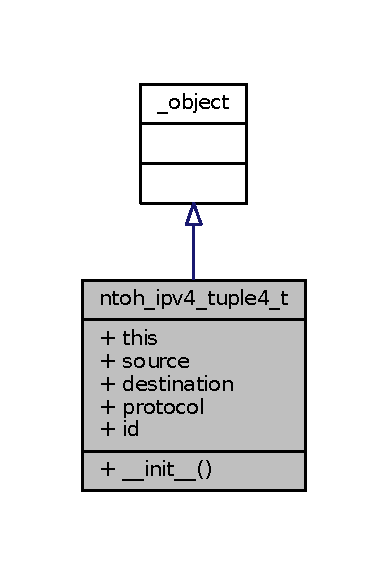
\includegraphics[width=186pt]{classlibntoh_1_1ntoh__ipv4__tuple4__t__inherit__graph}
\end{center}
\end{figure}


Collaboration diagram for ntoh\-\_\-ipv4\-\_\-tuple4\-\_\-t\-:
\nopagebreak
\begin{figure}[H]
\begin{center}
\leavevmode
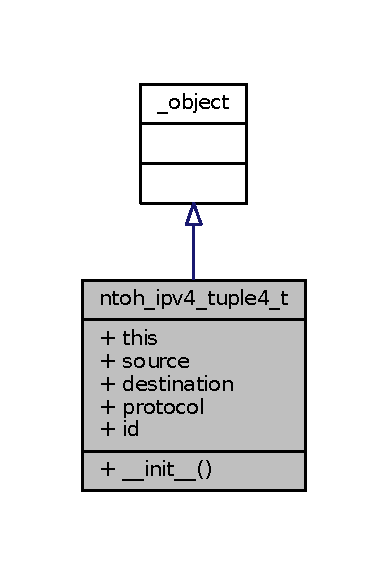
\includegraphics[width=186pt]{classlibntoh_1_1ntoh__ipv4__tuple4__t__coll__graph}
\end{center}
\end{figure}
\subsection*{Public Member Functions}
\begin{DoxyCompactItemize}
\item 
def \hyperlink{classlibntoh_1_1ntoh__ipv4__tuple4__t_ac775ee34451fdfa742b318538164070e}{\-\_\-\-\_\-init\-\_\-\-\_\-}
\end{DoxyCompactItemize}
\subsection*{Data Fields}
\begin{DoxyCompactItemize}
\item 
\hyperlink{classlibntoh_1_1ntoh__ipv4__tuple4__t_a05c09a5e9d53fa7adf0a7936038c2fa3}{this}
\end{DoxyCompactItemize}
\subsection*{Static Public Attributes}
\begin{DoxyCompactItemize}
\item 
tuple \hyperlink{classlibntoh_1_1ntoh__ipv4__tuple4__t_aa873026052cc3e5ba03877243fcb7ecd}{source} = \hyperlink{namespacelibntoh_ae6f5626f776538e0cdb00e75ca1c96c9}{\-\_\-swig\-\_\-property}(\-\_\-libntoh.\-ntoh\-\_\-ipv4\-\_\-tuple4\-\_\-t\-\_\-source\-\_\-get, \-\_\-libntoh.\-ntoh\-\_\-ipv4\-\_\-tuple4\-\_\-t\-\_\-source\-\_\-set)
\item 
tuple \hyperlink{classlibntoh_1_1ntoh__ipv4__tuple4__t_adaac82457baf1096d1c38cadf8123ce7}{destination} = \hyperlink{namespacelibntoh_ae6f5626f776538e0cdb00e75ca1c96c9}{\-\_\-swig\-\_\-property}(\-\_\-libntoh.\-ntoh\-\_\-ipv4\-\_\-tuple4\-\_\-t\-\_\-destination\-\_\-get, \-\_\-libntoh.\-ntoh\-\_\-ipv4\-\_\-tuple4\-\_\-t\-\_\-destination\-\_\-set)
\item 
tuple \hyperlink{classlibntoh_1_1ntoh__ipv4__tuple4__t_ae535ff0dd346855882bd298a9e22bbc1}{protocol} = \hyperlink{namespacelibntoh_ae6f5626f776538e0cdb00e75ca1c96c9}{\-\_\-swig\-\_\-property}(\-\_\-libntoh.\-ntoh\-\_\-ipv4\-\_\-tuple4\-\_\-t\-\_\-protocol\-\_\-get, \-\_\-libntoh.\-ntoh\-\_\-ipv4\-\_\-tuple4\-\_\-t\-\_\-protocol\-\_\-set)
\item 
tuple \hyperlink{classlibntoh_1_1ntoh__ipv4__tuple4__t_a0e43f6071072440917ee2dd8af07d251}{id} = \hyperlink{namespacelibntoh_ae6f5626f776538e0cdb00e75ca1c96c9}{\-\_\-swig\-\_\-property}(\-\_\-libntoh.\-ntoh\-\_\-ipv4\-\_\-tuple4\-\_\-t\-\_\-id\-\_\-get, \-\_\-libntoh.\-ntoh\-\_\-ipv4\-\_\-tuple4\-\_\-t\-\_\-id\-\_\-set)
\end{DoxyCompactItemize}


\subsection{Constructor \& Destructor Documentation}
\hypertarget{classlibntoh_1_1ntoh__ipv4__tuple4__t_ac775ee34451fdfa742b318538164070e}{\index{libntoh\-::ntoh\-\_\-ipv4\-\_\-tuple4\-\_\-t@{libntoh\-::ntoh\-\_\-ipv4\-\_\-tuple4\-\_\-t}!\-\_\-\-\_\-init\-\_\-\-\_\-@{\-\_\-\-\_\-init\-\_\-\-\_\-}}
\index{\-\_\-\-\_\-init\-\_\-\-\_\-@{\-\_\-\-\_\-init\-\_\-\-\_\-}!libntoh::ntoh_ipv4_tuple4_t@{libntoh\-::ntoh\-\_\-ipv4\-\_\-tuple4\-\_\-t}}
\subsubsection[{\-\_\-\-\_\-init\-\_\-\-\_\-}]{\setlength{\rightskip}{0pt plus 5cm}def \-\_\-\-\_\-init\-\_\-\-\_\- (
\begin{DoxyParamCaption}
\item[{}]{self}
\end{DoxyParamCaption}
)}}\label{classlibntoh_1_1ntoh__ipv4__tuple4__t_ac775ee34451fdfa742b318538164070e}


\subsection{Field Documentation}
\hypertarget{classlibntoh_1_1ntoh__ipv4__tuple4__t_adaac82457baf1096d1c38cadf8123ce7}{\index{libntoh\-::ntoh\-\_\-ipv4\-\_\-tuple4\-\_\-t@{libntoh\-::ntoh\-\_\-ipv4\-\_\-tuple4\-\_\-t}!destination@{destination}}
\index{destination@{destination}!libntoh::ntoh_ipv4_tuple4_t@{libntoh\-::ntoh\-\_\-ipv4\-\_\-tuple4\-\_\-t}}
\subsubsection[{destination}]{\setlength{\rightskip}{0pt plus 5cm}tuple destination = {\bf \-\_\-swig\-\_\-property}(\-\_\-libntoh.\-ntoh\-\_\-ipv4\-\_\-tuple4\-\_\-t\-\_\-destination\-\_\-get, \-\_\-libntoh.\-ntoh\-\_\-ipv4\-\_\-tuple4\-\_\-t\-\_\-destination\-\_\-set)\hspace{0.3cm}{\ttfamily [static]}}}\label{classlibntoh_1_1ntoh__ipv4__tuple4__t_adaac82457baf1096d1c38cadf8123ce7}
\hypertarget{classlibntoh_1_1ntoh__ipv4__tuple4__t_a0e43f6071072440917ee2dd8af07d251}{\index{libntoh\-::ntoh\-\_\-ipv4\-\_\-tuple4\-\_\-t@{libntoh\-::ntoh\-\_\-ipv4\-\_\-tuple4\-\_\-t}!id@{id}}
\index{id@{id}!libntoh::ntoh_ipv4_tuple4_t@{libntoh\-::ntoh\-\_\-ipv4\-\_\-tuple4\-\_\-t}}
\subsubsection[{id}]{\setlength{\rightskip}{0pt plus 5cm}tuple id = {\bf \-\_\-swig\-\_\-property}(\-\_\-libntoh.\-ntoh\-\_\-ipv4\-\_\-tuple4\-\_\-t\-\_\-id\-\_\-get, \-\_\-libntoh.\-ntoh\-\_\-ipv4\-\_\-tuple4\-\_\-t\-\_\-id\-\_\-set)\hspace{0.3cm}{\ttfamily [static]}}}\label{classlibntoh_1_1ntoh__ipv4__tuple4__t_a0e43f6071072440917ee2dd8af07d251}
\hypertarget{classlibntoh_1_1ntoh__ipv4__tuple4__t_ae535ff0dd346855882bd298a9e22bbc1}{\index{libntoh\-::ntoh\-\_\-ipv4\-\_\-tuple4\-\_\-t@{libntoh\-::ntoh\-\_\-ipv4\-\_\-tuple4\-\_\-t}!protocol@{protocol}}
\index{protocol@{protocol}!libntoh::ntoh_ipv4_tuple4_t@{libntoh\-::ntoh\-\_\-ipv4\-\_\-tuple4\-\_\-t}}
\subsubsection[{protocol}]{\setlength{\rightskip}{0pt plus 5cm}tuple protocol = {\bf \-\_\-swig\-\_\-property}(\-\_\-libntoh.\-ntoh\-\_\-ipv4\-\_\-tuple4\-\_\-t\-\_\-protocol\-\_\-get, \-\_\-libntoh.\-ntoh\-\_\-ipv4\-\_\-tuple4\-\_\-t\-\_\-protocol\-\_\-set)\hspace{0.3cm}{\ttfamily [static]}}}\label{classlibntoh_1_1ntoh__ipv4__tuple4__t_ae535ff0dd346855882bd298a9e22bbc1}
\hypertarget{classlibntoh_1_1ntoh__ipv4__tuple4__t_aa873026052cc3e5ba03877243fcb7ecd}{\index{libntoh\-::ntoh\-\_\-ipv4\-\_\-tuple4\-\_\-t@{libntoh\-::ntoh\-\_\-ipv4\-\_\-tuple4\-\_\-t}!source@{source}}
\index{source@{source}!libntoh::ntoh_ipv4_tuple4_t@{libntoh\-::ntoh\-\_\-ipv4\-\_\-tuple4\-\_\-t}}
\subsubsection[{source}]{\setlength{\rightskip}{0pt plus 5cm}tuple source = {\bf \-\_\-swig\-\_\-property}(\-\_\-libntoh.\-ntoh\-\_\-ipv4\-\_\-tuple4\-\_\-t\-\_\-source\-\_\-get, \-\_\-libntoh.\-ntoh\-\_\-ipv4\-\_\-tuple4\-\_\-t\-\_\-source\-\_\-set)\hspace{0.3cm}{\ttfamily [static]}}}\label{classlibntoh_1_1ntoh__ipv4__tuple4__t_aa873026052cc3e5ba03877243fcb7ecd}
\hypertarget{classlibntoh_1_1ntoh__ipv4__tuple4__t_a05c09a5e9d53fa7adf0a7936038c2fa3}{\index{libntoh\-::ntoh\-\_\-ipv4\-\_\-tuple4\-\_\-t@{libntoh\-::ntoh\-\_\-ipv4\-\_\-tuple4\-\_\-t}!this@{this}}
\index{this@{this}!libntoh::ntoh_ipv4_tuple4_t@{libntoh\-::ntoh\-\_\-ipv4\-\_\-tuple4\-\_\-t}}
\subsubsection[{this}]{\setlength{\rightskip}{0pt plus 5cm}this}}\label{classlibntoh_1_1ntoh__ipv4__tuple4__t_a05c09a5e9d53fa7adf0a7936038c2fa3}


The documentation for this class was generated from the following file\-:\begin{DoxyCompactItemize}
\item 
build/\hyperlink{libntoh_8py}{libntoh.\-py}\end{DoxyCompactItemize}

\hypertarget{structntoh__ipv4__tuple4__t}{\section{ntoh\-\_\-ipv4\-\_\-tuple4\-\_\-t Struct Reference}
\label{structntoh__ipv4__tuple4__t}\index{ntoh\-\_\-ipv4\-\_\-tuple4\-\_\-t@{ntoh\-\_\-ipv4\-\_\-tuple4\-\_\-t}}
}


Struct to generate the flow key.  




{\ttfamily \#include $<$ipv4defrag.\-h$>$}



Collaboration diagram for ntoh\-\_\-ipv4\-\_\-tuple4\-\_\-t\-:
\nopagebreak
\begin{figure}[H]
\begin{center}
\leavevmode
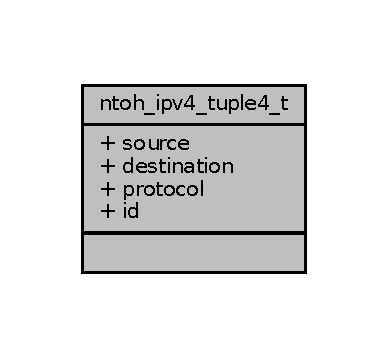
\includegraphics[width=186pt]{structntoh__ipv4__tuple4__t__coll__graph}
\end{center}
\end{figure}
\subsection*{Data Fields}
\begin{DoxyCompactItemize}
\item 
unsigned int \hyperlink{structntoh__ipv4__tuple4__t_a32ee136f9a3309d9f5aec70ddaebc420}{source}
\begin{DoxyCompactList}\small\item\em source I\-P address \end{DoxyCompactList}\item 
unsigned int \hyperlink{structntoh__ipv4__tuple4__t_aa2b73075fb6a7866116ece24e01ea950}{destination}
\begin{DoxyCompactList}\small\item\em destination I\-P address \end{DoxyCompactList}\item 
uint8\-\_\-t \hyperlink{structntoh__ipv4__tuple4__t_ad124d3d2e02c729afa303c775295278e}{protocol}
\begin{DoxyCompactList}\small\item\em Transport layer protocol. \end{DoxyCompactList}\item 
unsigned short \hyperlink{structntoh__ipv4__tuple4__t_a2e74aff868562e644e5d582929433363}{id}
\begin{DoxyCompactList}\small\item\em Identification. \end{DoxyCompactList}\end{DoxyCompactItemize}


\subsection{Detailed Description}
Struct to generate the flow key. 

\subsection{Field Documentation}
\hypertarget{structntoh__ipv4__tuple4__t_aa2b73075fb6a7866116ece24e01ea950}{\index{ntoh\-\_\-ipv4\-\_\-tuple4\-\_\-t@{ntoh\-\_\-ipv4\-\_\-tuple4\-\_\-t}!destination@{destination}}
\index{destination@{destination}!ntoh_ipv4_tuple4_t@{ntoh\-\_\-ipv4\-\_\-tuple4\-\_\-t}}
\subsubsection[{destination}]{\setlength{\rightskip}{0pt plus 5cm}unsigned int destination}}\label{structntoh__ipv4__tuple4__t_aa2b73075fb6a7866116ece24e01ea950}


destination I\-P address 

\hypertarget{structntoh__ipv4__tuple4__t_a2e74aff868562e644e5d582929433363}{\index{ntoh\-\_\-ipv4\-\_\-tuple4\-\_\-t@{ntoh\-\_\-ipv4\-\_\-tuple4\-\_\-t}!id@{id}}
\index{id@{id}!ntoh_ipv4_tuple4_t@{ntoh\-\_\-ipv4\-\_\-tuple4\-\_\-t}}
\subsubsection[{id}]{\setlength{\rightskip}{0pt plus 5cm}unsigned short id}}\label{structntoh__ipv4__tuple4__t_a2e74aff868562e644e5d582929433363}


Identification. 

\hypertarget{structntoh__ipv4__tuple4__t_ad124d3d2e02c729afa303c775295278e}{\index{ntoh\-\_\-ipv4\-\_\-tuple4\-\_\-t@{ntoh\-\_\-ipv4\-\_\-tuple4\-\_\-t}!protocol@{protocol}}
\index{protocol@{protocol}!ntoh_ipv4_tuple4_t@{ntoh\-\_\-ipv4\-\_\-tuple4\-\_\-t}}
\subsubsection[{protocol}]{\setlength{\rightskip}{0pt plus 5cm}uint8\-\_\-t protocol}}\label{structntoh__ipv4__tuple4__t_ad124d3d2e02c729afa303c775295278e}


Transport layer protocol. 

\hypertarget{structntoh__ipv4__tuple4__t_a32ee136f9a3309d9f5aec70ddaebc420}{\index{ntoh\-\_\-ipv4\-\_\-tuple4\-\_\-t@{ntoh\-\_\-ipv4\-\_\-tuple4\-\_\-t}!source@{source}}
\index{source@{source}!ntoh_ipv4_tuple4_t@{ntoh\-\_\-ipv4\-\_\-tuple4\-\_\-t}}
\subsubsection[{source}]{\setlength{\rightskip}{0pt plus 5cm}unsigned int source}}\label{structntoh__ipv4__tuple4__t_a32ee136f9a3309d9f5aec70ddaebc420}


source I\-P address 



The documentation for this struct was generated from the following file\-:\begin{DoxyCompactItemize}
\item 
inc/\hyperlink{ipv4defrag_8h}{ipv4defrag.\-h}\end{DoxyCompactItemize}

\hypertarget{structntoh__ipv6__flow__t}{\section{ntoh\-\_\-ipv6\-\_\-flow\-\_\-t Struct Reference}
\label{structntoh__ipv6__flow__t}\index{ntoh\-\_\-ipv6\-\_\-flow\-\_\-t@{ntoh\-\_\-ipv6\-\_\-flow\-\_\-t}}
}


Struct to store the information of each I\-Pv6 flow.  




{\ttfamily \#include $<$ipv6defrag.\-h$>$}



Collaboration diagram for ntoh\-\_\-ipv6\-\_\-flow\-\_\-t\-:
\nopagebreak
\begin{figure}[H]
\begin{center}
\leavevmode
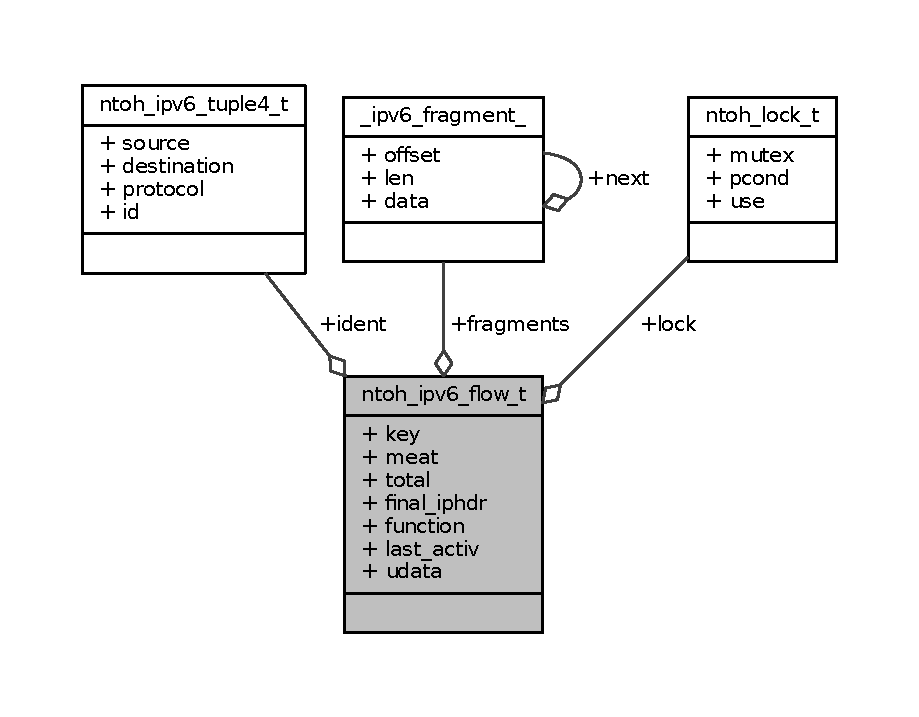
\includegraphics[width=350pt]{structntoh__ipv6__flow__t__coll__graph}
\end{center}
\end{figure}
\subsection*{Data Fields}
\begin{DoxyCompactItemize}
\item 
\hyperlink{structntoh__ipv6__tuple4__t}{ntoh\-\_\-ipv6\-\_\-tuple4\-\_\-t} \hyperlink{structntoh__ipv6__flow__t_ae6f21eaeed6948ec645d7d94a37c3140}{ident}
\begin{DoxyCompactList}\small\item\em flow identification data \end{DoxyCompactList}\item 
\hyperlink{ipv6defrag_8h_a078ba881dae0588c609a3556dc5909ca}{ntoh\-\_\-ipv6\-\_\-key\-\_\-t} \hyperlink{structntoh__ipv6__flow__t_a8c3b4b46820e7d3e3af76db78a1dbb3e}{key}
\begin{DoxyCompactList}\small\item\em flow key \end{DoxyCompactList}\item 
\hyperlink{ipv6defrag_8h_ae909c7bd6d9a37597f561a92ab1ba2a7}{pntoh\-\_\-ipv6\-\_\-fragment\-\_\-t} \hyperlink{structntoh__ipv6__flow__t_abecfe5b83d9c9dfb2815e0579ea909fc}{fragments}
\begin{DoxyCompactList}\small\item\em fragments list \end{DoxyCompactList}\item 
size\-\_\-t \hyperlink{structntoh__ipv6__flow__t_a25cdc91a1ce3b46649beaacf6315dee7}{meat}
\begin{DoxyCompactList}\small\item\em total amount of received data \end{DoxyCompactList}\item 
size\-\_\-t \hyperlink{structntoh__ipv6__flow__t_a3fab45bb4d7cd7e889bdf00080096e8e}{total}
\begin{DoxyCompactList}\small\item\em total amount of expected data \end{DoxyCompactList}\item 
struct ip6\-\_\-hdr $\ast$ \hyperlink{structntoh__ipv6__flow__t_aacadfda29e478e69be73c3f2e6bf9c79}{final\-\_\-iphdr}
\begin{DoxyCompactList}\small\item\em final fragment received? \end{DoxyCompactList}\item 
void $\ast$ \hyperlink{structntoh__ipv6__flow__t_aea3dcf0c8de30d192ee92494131c4996}{function}
\begin{DoxyCompactList}\small\item\em user defined function to receive defragmented packets \end{DoxyCompactList}\item 
struct timeval \hyperlink{structntoh__ipv6__flow__t_a9d115049a50ba4e69eb04c23c973a4a2}{last\-\_\-activ}
\begin{DoxyCompactList}\small\item\em last activity \end{DoxyCompactList}\item 
void $\ast$ \hyperlink{structntoh__ipv6__flow__t_a697ce711b67313990d351b5c95f87aed}{udata}
\begin{DoxyCompactList}\small\item\em user-\/defined data \end{DoxyCompactList}\item 
\hyperlink{structntoh__lock__t}{ntoh\-\_\-lock\-\_\-t} \hyperlink{structntoh__ipv6__flow__t_aad15823e4f2835531e6a02321cd53f7e}{lock}
\end{DoxyCompactItemize}


\subsection{Detailed Description}
Struct to store the information of each I\-Pv6 flow. 

\subsection{Field Documentation}
\hypertarget{structntoh__ipv6__flow__t_aacadfda29e478e69be73c3f2e6bf9c79}{\index{ntoh\-\_\-ipv6\-\_\-flow\-\_\-t@{ntoh\-\_\-ipv6\-\_\-flow\-\_\-t}!final\-\_\-iphdr@{final\-\_\-iphdr}}
\index{final\-\_\-iphdr@{final\-\_\-iphdr}!ntoh_ipv6_flow_t@{ntoh\-\_\-ipv6\-\_\-flow\-\_\-t}}
\subsubsection[{final\-\_\-iphdr}]{\setlength{\rightskip}{0pt plus 5cm}struct ip6\-\_\-hdr$\ast$ final\-\_\-iphdr}}\label{structntoh__ipv6__flow__t_aacadfda29e478e69be73c3f2e6bf9c79}


final fragment received? 

\hypertarget{structntoh__ipv6__flow__t_abecfe5b83d9c9dfb2815e0579ea909fc}{\index{ntoh\-\_\-ipv6\-\_\-flow\-\_\-t@{ntoh\-\_\-ipv6\-\_\-flow\-\_\-t}!fragments@{fragments}}
\index{fragments@{fragments}!ntoh_ipv6_flow_t@{ntoh\-\_\-ipv6\-\_\-flow\-\_\-t}}
\subsubsection[{fragments}]{\setlength{\rightskip}{0pt plus 5cm}{\bf pntoh\-\_\-ipv6\-\_\-fragment\-\_\-t} fragments}}\label{structntoh__ipv6__flow__t_abecfe5b83d9c9dfb2815e0579ea909fc}


fragments list 

\hypertarget{structntoh__ipv6__flow__t_aea3dcf0c8de30d192ee92494131c4996}{\index{ntoh\-\_\-ipv6\-\_\-flow\-\_\-t@{ntoh\-\_\-ipv6\-\_\-flow\-\_\-t}!function@{function}}
\index{function@{function}!ntoh_ipv6_flow_t@{ntoh\-\_\-ipv6\-\_\-flow\-\_\-t}}
\subsubsection[{function}]{\setlength{\rightskip}{0pt plus 5cm}void$\ast$ function}}\label{structntoh__ipv6__flow__t_aea3dcf0c8de30d192ee92494131c4996}


user defined function to receive defragmented packets 

\hypertarget{structntoh__ipv6__flow__t_ae6f21eaeed6948ec645d7d94a37c3140}{\index{ntoh\-\_\-ipv6\-\_\-flow\-\_\-t@{ntoh\-\_\-ipv6\-\_\-flow\-\_\-t}!ident@{ident}}
\index{ident@{ident}!ntoh_ipv6_flow_t@{ntoh\-\_\-ipv6\-\_\-flow\-\_\-t}}
\subsubsection[{ident}]{\setlength{\rightskip}{0pt plus 5cm}{\bf ntoh\-\_\-ipv6\-\_\-tuple4\-\_\-t} ident}}\label{structntoh__ipv6__flow__t_ae6f21eaeed6948ec645d7d94a37c3140}


flow identification data 

\hypertarget{structntoh__ipv6__flow__t_a8c3b4b46820e7d3e3af76db78a1dbb3e}{\index{ntoh\-\_\-ipv6\-\_\-flow\-\_\-t@{ntoh\-\_\-ipv6\-\_\-flow\-\_\-t}!key@{key}}
\index{key@{key}!ntoh_ipv6_flow_t@{ntoh\-\_\-ipv6\-\_\-flow\-\_\-t}}
\subsubsection[{key}]{\setlength{\rightskip}{0pt plus 5cm}{\bf ntoh\-\_\-ipv6\-\_\-key\-\_\-t} key}}\label{structntoh__ipv6__flow__t_a8c3b4b46820e7d3e3af76db78a1dbb3e}


flow key 

\hypertarget{structntoh__ipv6__flow__t_a9d115049a50ba4e69eb04c23c973a4a2}{\index{ntoh\-\_\-ipv6\-\_\-flow\-\_\-t@{ntoh\-\_\-ipv6\-\_\-flow\-\_\-t}!last\-\_\-activ@{last\-\_\-activ}}
\index{last\-\_\-activ@{last\-\_\-activ}!ntoh_ipv6_flow_t@{ntoh\-\_\-ipv6\-\_\-flow\-\_\-t}}
\subsubsection[{last\-\_\-activ}]{\setlength{\rightskip}{0pt plus 5cm}struct timeval last\-\_\-activ}}\label{structntoh__ipv6__flow__t_a9d115049a50ba4e69eb04c23c973a4a2}


last activity 

\hypertarget{structntoh__ipv6__flow__t_aad15823e4f2835531e6a02321cd53f7e}{\index{ntoh\-\_\-ipv6\-\_\-flow\-\_\-t@{ntoh\-\_\-ipv6\-\_\-flow\-\_\-t}!lock@{lock}}
\index{lock@{lock}!ntoh_ipv6_flow_t@{ntoh\-\_\-ipv6\-\_\-flow\-\_\-t}}
\subsubsection[{lock}]{\setlength{\rightskip}{0pt plus 5cm}{\bf ntoh\-\_\-lock\-\_\-t} lock}}\label{structntoh__ipv6__flow__t_aad15823e4f2835531e6a02321cd53f7e}
\hypertarget{structntoh__ipv6__flow__t_a25cdc91a1ce3b46649beaacf6315dee7}{\index{ntoh\-\_\-ipv6\-\_\-flow\-\_\-t@{ntoh\-\_\-ipv6\-\_\-flow\-\_\-t}!meat@{meat}}
\index{meat@{meat}!ntoh_ipv6_flow_t@{ntoh\-\_\-ipv6\-\_\-flow\-\_\-t}}
\subsubsection[{meat}]{\setlength{\rightskip}{0pt plus 5cm}size\-\_\-t meat}}\label{structntoh__ipv6__flow__t_a25cdc91a1ce3b46649beaacf6315dee7}


total amount of received data 

\hypertarget{structntoh__ipv6__flow__t_a3fab45bb4d7cd7e889bdf00080096e8e}{\index{ntoh\-\_\-ipv6\-\_\-flow\-\_\-t@{ntoh\-\_\-ipv6\-\_\-flow\-\_\-t}!total@{total}}
\index{total@{total}!ntoh_ipv6_flow_t@{ntoh\-\_\-ipv6\-\_\-flow\-\_\-t}}
\subsubsection[{total}]{\setlength{\rightskip}{0pt plus 5cm}size\-\_\-t total}}\label{structntoh__ipv6__flow__t_a3fab45bb4d7cd7e889bdf00080096e8e}


total amount of expected data 

\hypertarget{structntoh__ipv6__flow__t_a697ce711b67313990d351b5c95f87aed}{\index{ntoh\-\_\-ipv6\-\_\-flow\-\_\-t@{ntoh\-\_\-ipv6\-\_\-flow\-\_\-t}!udata@{udata}}
\index{udata@{udata}!ntoh_ipv6_flow_t@{ntoh\-\_\-ipv6\-\_\-flow\-\_\-t}}
\subsubsection[{udata}]{\setlength{\rightskip}{0pt plus 5cm}void$\ast$ udata}}\label{structntoh__ipv6__flow__t_a697ce711b67313990d351b5c95f87aed}


user-\/defined data 



The documentation for this struct was generated from the following file\-:\begin{DoxyCompactItemize}
\item 
inc/\hyperlink{ipv6defrag_8h}{ipv6defrag.\-h}\end{DoxyCompactItemize}

\hypertarget{classlibntoh_1_1ntoh__ipv6__flow__t}{\section{ntoh\-\_\-ipv6\-\_\-flow\-\_\-t Class Reference}
\label{classlibntoh_1_1ntoh__ipv6__flow__t}\index{ntoh\-\_\-ipv6\-\_\-flow\-\_\-t@{ntoh\-\_\-ipv6\-\_\-flow\-\_\-t}}
}


Inheritance diagram for ntoh\-\_\-ipv6\-\_\-flow\-\_\-t\-:
\nopagebreak
\begin{figure}[H]
\begin{center}
\leavevmode
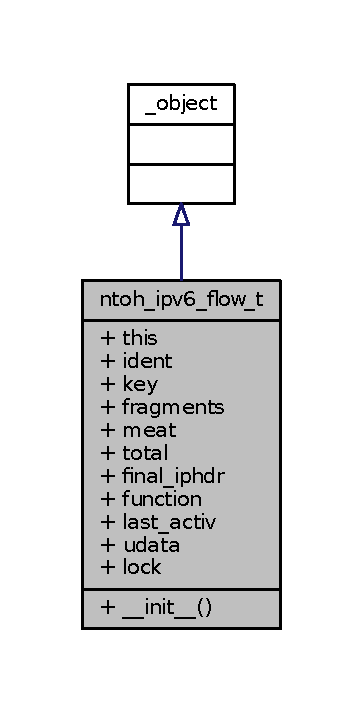
\includegraphics[width=174pt]{classlibntoh_1_1ntoh__ipv6__flow__t__inherit__graph}
\end{center}
\end{figure}


Collaboration diagram for ntoh\-\_\-ipv6\-\_\-flow\-\_\-t\-:
\nopagebreak
\begin{figure}[H]
\begin{center}
\leavevmode
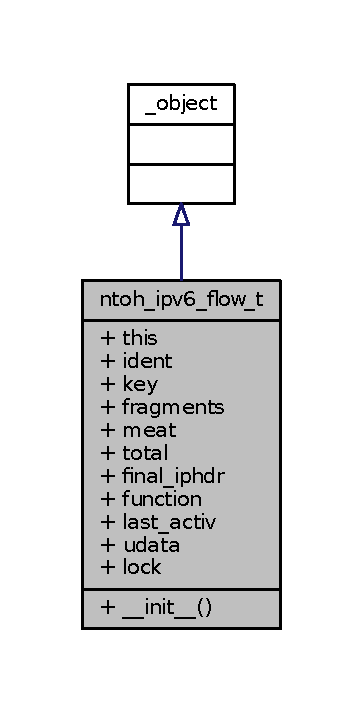
\includegraphics[width=174pt]{classlibntoh_1_1ntoh__ipv6__flow__t__coll__graph}
\end{center}
\end{figure}
\subsection*{Public Member Functions}
\begin{DoxyCompactItemize}
\item 
def \hyperlink{classlibntoh_1_1ntoh__ipv6__flow__t_ac775ee34451fdfa742b318538164070e}{\-\_\-\-\_\-init\-\_\-\-\_\-}
\end{DoxyCompactItemize}
\subsection*{Data Fields}
\begin{DoxyCompactItemize}
\item 
\hyperlink{classlibntoh_1_1ntoh__ipv6__flow__t_a05c09a5e9d53fa7adf0a7936038c2fa3}{this}
\end{DoxyCompactItemize}
\subsection*{Static Public Attributes}
\begin{DoxyCompactItemize}
\item 
tuple \hyperlink{classlibntoh_1_1ntoh__ipv6__flow__t_a219b3ba79a48452030ad36cf2519ee85}{ident} = \hyperlink{namespacelibntoh_ae6f5626f776538e0cdb00e75ca1c96c9}{\-\_\-swig\-\_\-property}(\-\_\-libntoh.\-ntoh\-\_\-ipv6\-\_\-flow\-\_\-t\-\_\-ident\-\_\-get, \-\_\-libntoh.\-ntoh\-\_\-ipv6\-\_\-flow\-\_\-t\-\_\-ident\-\_\-set)
\item 
tuple \hyperlink{classlibntoh_1_1ntoh__ipv6__flow__t_a29eb8dd921f77e19e24a20bcd820c2ed}{key} = \hyperlink{namespacelibntoh_ae6f5626f776538e0cdb00e75ca1c96c9}{\-\_\-swig\-\_\-property}(\-\_\-libntoh.\-ntoh\-\_\-ipv6\-\_\-flow\-\_\-t\-\_\-key\-\_\-get, \-\_\-libntoh.\-ntoh\-\_\-ipv6\-\_\-flow\-\_\-t\-\_\-key\-\_\-set)
\item 
tuple \hyperlink{classlibntoh_1_1ntoh__ipv6__flow__t_a61a562f6a662704721df2bd666792d24}{fragments} = \hyperlink{namespacelibntoh_ae6f5626f776538e0cdb00e75ca1c96c9}{\-\_\-swig\-\_\-property}(\-\_\-libntoh.\-ntoh\-\_\-ipv6\-\_\-flow\-\_\-t\-\_\-fragments\-\_\-get, \-\_\-libntoh.\-ntoh\-\_\-ipv6\-\_\-flow\-\_\-t\-\_\-fragments\-\_\-set)
\item 
tuple \hyperlink{classlibntoh_1_1ntoh__ipv6__flow__t_a05f7a909b2438fcd11159037a9b76457}{meat} = \hyperlink{namespacelibntoh_ae6f5626f776538e0cdb00e75ca1c96c9}{\-\_\-swig\-\_\-property}(\-\_\-libntoh.\-ntoh\-\_\-ipv6\-\_\-flow\-\_\-t\-\_\-meat\-\_\-get, \-\_\-libntoh.\-ntoh\-\_\-ipv6\-\_\-flow\-\_\-t\-\_\-meat\-\_\-set)
\item 
tuple \hyperlink{classlibntoh_1_1ntoh__ipv6__flow__t_a707ba789fae19e34fbeeca4da8c30c5f}{total} = \hyperlink{namespacelibntoh_ae6f5626f776538e0cdb00e75ca1c96c9}{\-\_\-swig\-\_\-property}(\-\_\-libntoh.\-ntoh\-\_\-ipv6\-\_\-flow\-\_\-t\-\_\-total\-\_\-get, \-\_\-libntoh.\-ntoh\-\_\-ipv6\-\_\-flow\-\_\-t\-\_\-total\-\_\-set)
\item 
tuple \hyperlink{classlibntoh_1_1ntoh__ipv6__flow__t_aaae262685d5063d60668907a4beaf956}{final\-\_\-iphdr} = \hyperlink{namespacelibntoh_ae6f5626f776538e0cdb00e75ca1c96c9}{\-\_\-swig\-\_\-property}(\-\_\-libntoh.\-ntoh\-\_\-ipv6\-\_\-flow\-\_\-t\-\_\-final\-\_\-iphdr\-\_\-get, \-\_\-libntoh.\-ntoh\-\_\-ipv6\-\_\-flow\-\_\-t\-\_\-final\-\_\-iphdr\-\_\-set)
\item 
tuple \hyperlink{classlibntoh_1_1ntoh__ipv6__flow__t_a543077174a1281b9d00884a11a040629}{function} = \hyperlink{namespacelibntoh_ae6f5626f776538e0cdb00e75ca1c96c9}{\-\_\-swig\-\_\-property}(\-\_\-libntoh.\-ntoh\-\_\-ipv6\-\_\-flow\-\_\-t\-\_\-function\-\_\-get, \-\_\-libntoh.\-ntoh\-\_\-ipv6\-\_\-flow\-\_\-t\-\_\-function\-\_\-set)
\item 
tuple \hyperlink{classlibntoh_1_1ntoh__ipv6__flow__t_a43a06ba72aed8671dd1579dbf6f78b1a}{last\-\_\-activ} = \hyperlink{namespacelibntoh_ae6f5626f776538e0cdb00e75ca1c96c9}{\-\_\-swig\-\_\-property}(\-\_\-libntoh.\-ntoh\-\_\-ipv6\-\_\-flow\-\_\-t\-\_\-last\-\_\-activ\-\_\-get, \-\_\-libntoh.\-ntoh\-\_\-ipv6\-\_\-flow\-\_\-t\-\_\-last\-\_\-activ\-\_\-set)
\item 
tuple \hyperlink{classlibntoh_1_1ntoh__ipv6__flow__t_a6900744e840ca75a67e020c38d143891}{udata} = \hyperlink{namespacelibntoh_ae6f5626f776538e0cdb00e75ca1c96c9}{\-\_\-swig\-\_\-property}(\-\_\-libntoh.\-ntoh\-\_\-ipv6\-\_\-flow\-\_\-t\-\_\-udata\-\_\-get, \-\_\-libntoh.\-ntoh\-\_\-ipv6\-\_\-flow\-\_\-t\-\_\-udata\-\_\-set)
\item 
tuple \hyperlink{classlibntoh_1_1ntoh__ipv6__flow__t_a871c7bf899334194698c2a3bced5e064}{lock} = \hyperlink{namespacelibntoh_ae6f5626f776538e0cdb00e75ca1c96c9}{\-\_\-swig\-\_\-property}(\-\_\-libntoh.\-ntoh\-\_\-ipv6\-\_\-flow\-\_\-t\-\_\-lock\-\_\-get, \-\_\-libntoh.\-ntoh\-\_\-ipv6\-\_\-flow\-\_\-t\-\_\-lock\-\_\-set)
\end{DoxyCompactItemize}


\subsection{Constructor \& Destructor Documentation}
\hypertarget{classlibntoh_1_1ntoh__ipv6__flow__t_ac775ee34451fdfa742b318538164070e}{\index{libntoh\-::ntoh\-\_\-ipv6\-\_\-flow\-\_\-t@{libntoh\-::ntoh\-\_\-ipv6\-\_\-flow\-\_\-t}!\-\_\-\-\_\-init\-\_\-\-\_\-@{\-\_\-\-\_\-init\-\_\-\-\_\-}}
\index{\-\_\-\-\_\-init\-\_\-\-\_\-@{\-\_\-\-\_\-init\-\_\-\-\_\-}!libntoh::ntoh_ipv6_flow_t@{libntoh\-::ntoh\-\_\-ipv6\-\_\-flow\-\_\-t}}
\subsubsection[{\-\_\-\-\_\-init\-\_\-\-\_\-}]{\setlength{\rightskip}{0pt plus 5cm}def \-\_\-\-\_\-init\-\_\-\-\_\- (
\begin{DoxyParamCaption}
\item[{}]{self}
\end{DoxyParamCaption}
)}}\label{classlibntoh_1_1ntoh__ipv6__flow__t_ac775ee34451fdfa742b318538164070e}


\subsection{Field Documentation}
\hypertarget{classlibntoh_1_1ntoh__ipv6__flow__t_aaae262685d5063d60668907a4beaf956}{\index{libntoh\-::ntoh\-\_\-ipv6\-\_\-flow\-\_\-t@{libntoh\-::ntoh\-\_\-ipv6\-\_\-flow\-\_\-t}!final\-\_\-iphdr@{final\-\_\-iphdr}}
\index{final\-\_\-iphdr@{final\-\_\-iphdr}!libntoh::ntoh_ipv6_flow_t@{libntoh\-::ntoh\-\_\-ipv6\-\_\-flow\-\_\-t}}
\subsubsection[{final\-\_\-iphdr}]{\setlength{\rightskip}{0pt plus 5cm}tuple final\-\_\-iphdr = {\bf \-\_\-swig\-\_\-property}(\-\_\-libntoh.\-ntoh\-\_\-ipv6\-\_\-flow\-\_\-t\-\_\-final\-\_\-iphdr\-\_\-get, \-\_\-libntoh.\-ntoh\-\_\-ipv6\-\_\-flow\-\_\-t\-\_\-final\-\_\-iphdr\-\_\-set)\hspace{0.3cm}{\ttfamily [static]}}}\label{classlibntoh_1_1ntoh__ipv6__flow__t_aaae262685d5063d60668907a4beaf956}
\hypertarget{classlibntoh_1_1ntoh__ipv6__flow__t_a61a562f6a662704721df2bd666792d24}{\index{libntoh\-::ntoh\-\_\-ipv6\-\_\-flow\-\_\-t@{libntoh\-::ntoh\-\_\-ipv6\-\_\-flow\-\_\-t}!fragments@{fragments}}
\index{fragments@{fragments}!libntoh::ntoh_ipv6_flow_t@{libntoh\-::ntoh\-\_\-ipv6\-\_\-flow\-\_\-t}}
\subsubsection[{fragments}]{\setlength{\rightskip}{0pt plus 5cm}tuple fragments = {\bf \-\_\-swig\-\_\-property}(\-\_\-libntoh.\-ntoh\-\_\-ipv6\-\_\-flow\-\_\-t\-\_\-fragments\-\_\-get, \-\_\-libntoh.\-ntoh\-\_\-ipv6\-\_\-flow\-\_\-t\-\_\-fragments\-\_\-set)\hspace{0.3cm}{\ttfamily [static]}}}\label{classlibntoh_1_1ntoh__ipv6__flow__t_a61a562f6a662704721df2bd666792d24}
\hypertarget{classlibntoh_1_1ntoh__ipv6__flow__t_a543077174a1281b9d00884a11a040629}{\index{libntoh\-::ntoh\-\_\-ipv6\-\_\-flow\-\_\-t@{libntoh\-::ntoh\-\_\-ipv6\-\_\-flow\-\_\-t}!function@{function}}
\index{function@{function}!libntoh::ntoh_ipv6_flow_t@{libntoh\-::ntoh\-\_\-ipv6\-\_\-flow\-\_\-t}}
\subsubsection[{function}]{\setlength{\rightskip}{0pt plus 5cm}tuple function = {\bf \-\_\-swig\-\_\-property}(\-\_\-libntoh.\-ntoh\-\_\-ipv6\-\_\-flow\-\_\-t\-\_\-function\-\_\-get, \-\_\-libntoh.\-ntoh\-\_\-ipv6\-\_\-flow\-\_\-t\-\_\-function\-\_\-set)\hspace{0.3cm}{\ttfamily [static]}}}\label{classlibntoh_1_1ntoh__ipv6__flow__t_a543077174a1281b9d00884a11a040629}
\hypertarget{classlibntoh_1_1ntoh__ipv6__flow__t_a219b3ba79a48452030ad36cf2519ee85}{\index{libntoh\-::ntoh\-\_\-ipv6\-\_\-flow\-\_\-t@{libntoh\-::ntoh\-\_\-ipv6\-\_\-flow\-\_\-t}!ident@{ident}}
\index{ident@{ident}!libntoh::ntoh_ipv6_flow_t@{libntoh\-::ntoh\-\_\-ipv6\-\_\-flow\-\_\-t}}
\subsubsection[{ident}]{\setlength{\rightskip}{0pt plus 5cm}tuple ident = {\bf \-\_\-swig\-\_\-property}(\-\_\-libntoh.\-ntoh\-\_\-ipv6\-\_\-flow\-\_\-t\-\_\-ident\-\_\-get, \-\_\-libntoh.\-ntoh\-\_\-ipv6\-\_\-flow\-\_\-t\-\_\-ident\-\_\-set)\hspace{0.3cm}{\ttfamily [static]}}}\label{classlibntoh_1_1ntoh__ipv6__flow__t_a219b3ba79a48452030ad36cf2519ee85}
\hypertarget{classlibntoh_1_1ntoh__ipv6__flow__t_a29eb8dd921f77e19e24a20bcd820c2ed}{\index{libntoh\-::ntoh\-\_\-ipv6\-\_\-flow\-\_\-t@{libntoh\-::ntoh\-\_\-ipv6\-\_\-flow\-\_\-t}!key@{key}}
\index{key@{key}!libntoh::ntoh_ipv6_flow_t@{libntoh\-::ntoh\-\_\-ipv6\-\_\-flow\-\_\-t}}
\subsubsection[{key}]{\setlength{\rightskip}{0pt plus 5cm}tuple key = {\bf \-\_\-swig\-\_\-property}(\-\_\-libntoh.\-ntoh\-\_\-ipv6\-\_\-flow\-\_\-t\-\_\-key\-\_\-get, \-\_\-libntoh.\-ntoh\-\_\-ipv6\-\_\-flow\-\_\-t\-\_\-key\-\_\-set)\hspace{0.3cm}{\ttfamily [static]}}}\label{classlibntoh_1_1ntoh__ipv6__flow__t_a29eb8dd921f77e19e24a20bcd820c2ed}
\hypertarget{classlibntoh_1_1ntoh__ipv6__flow__t_a43a06ba72aed8671dd1579dbf6f78b1a}{\index{libntoh\-::ntoh\-\_\-ipv6\-\_\-flow\-\_\-t@{libntoh\-::ntoh\-\_\-ipv6\-\_\-flow\-\_\-t}!last\-\_\-activ@{last\-\_\-activ}}
\index{last\-\_\-activ@{last\-\_\-activ}!libntoh::ntoh_ipv6_flow_t@{libntoh\-::ntoh\-\_\-ipv6\-\_\-flow\-\_\-t}}
\subsubsection[{last\-\_\-activ}]{\setlength{\rightskip}{0pt plus 5cm}tuple last\-\_\-activ = {\bf \-\_\-swig\-\_\-property}(\-\_\-libntoh.\-ntoh\-\_\-ipv6\-\_\-flow\-\_\-t\-\_\-last\-\_\-activ\-\_\-get, \-\_\-libntoh.\-ntoh\-\_\-ipv6\-\_\-flow\-\_\-t\-\_\-last\-\_\-activ\-\_\-set)\hspace{0.3cm}{\ttfamily [static]}}}\label{classlibntoh_1_1ntoh__ipv6__flow__t_a43a06ba72aed8671dd1579dbf6f78b1a}
\hypertarget{classlibntoh_1_1ntoh__ipv6__flow__t_a871c7bf899334194698c2a3bced5e064}{\index{libntoh\-::ntoh\-\_\-ipv6\-\_\-flow\-\_\-t@{libntoh\-::ntoh\-\_\-ipv6\-\_\-flow\-\_\-t}!lock@{lock}}
\index{lock@{lock}!libntoh::ntoh_ipv6_flow_t@{libntoh\-::ntoh\-\_\-ipv6\-\_\-flow\-\_\-t}}
\subsubsection[{lock}]{\setlength{\rightskip}{0pt plus 5cm}tuple lock = {\bf \-\_\-swig\-\_\-property}(\-\_\-libntoh.\-ntoh\-\_\-ipv6\-\_\-flow\-\_\-t\-\_\-lock\-\_\-get, \-\_\-libntoh.\-ntoh\-\_\-ipv6\-\_\-flow\-\_\-t\-\_\-lock\-\_\-set)\hspace{0.3cm}{\ttfamily [static]}}}\label{classlibntoh_1_1ntoh__ipv6__flow__t_a871c7bf899334194698c2a3bced5e064}
\hypertarget{classlibntoh_1_1ntoh__ipv6__flow__t_a05f7a909b2438fcd11159037a9b76457}{\index{libntoh\-::ntoh\-\_\-ipv6\-\_\-flow\-\_\-t@{libntoh\-::ntoh\-\_\-ipv6\-\_\-flow\-\_\-t}!meat@{meat}}
\index{meat@{meat}!libntoh::ntoh_ipv6_flow_t@{libntoh\-::ntoh\-\_\-ipv6\-\_\-flow\-\_\-t}}
\subsubsection[{meat}]{\setlength{\rightskip}{0pt plus 5cm}tuple meat = {\bf \-\_\-swig\-\_\-property}(\-\_\-libntoh.\-ntoh\-\_\-ipv6\-\_\-flow\-\_\-t\-\_\-meat\-\_\-get, \-\_\-libntoh.\-ntoh\-\_\-ipv6\-\_\-flow\-\_\-t\-\_\-meat\-\_\-set)\hspace{0.3cm}{\ttfamily [static]}}}\label{classlibntoh_1_1ntoh__ipv6__flow__t_a05f7a909b2438fcd11159037a9b76457}
\hypertarget{classlibntoh_1_1ntoh__ipv6__flow__t_a05c09a5e9d53fa7adf0a7936038c2fa3}{\index{libntoh\-::ntoh\-\_\-ipv6\-\_\-flow\-\_\-t@{libntoh\-::ntoh\-\_\-ipv6\-\_\-flow\-\_\-t}!this@{this}}
\index{this@{this}!libntoh::ntoh_ipv6_flow_t@{libntoh\-::ntoh\-\_\-ipv6\-\_\-flow\-\_\-t}}
\subsubsection[{this}]{\setlength{\rightskip}{0pt plus 5cm}this}}\label{classlibntoh_1_1ntoh__ipv6__flow__t_a05c09a5e9d53fa7adf0a7936038c2fa3}
\hypertarget{classlibntoh_1_1ntoh__ipv6__flow__t_a707ba789fae19e34fbeeca4da8c30c5f}{\index{libntoh\-::ntoh\-\_\-ipv6\-\_\-flow\-\_\-t@{libntoh\-::ntoh\-\_\-ipv6\-\_\-flow\-\_\-t}!total@{total}}
\index{total@{total}!libntoh::ntoh_ipv6_flow_t@{libntoh\-::ntoh\-\_\-ipv6\-\_\-flow\-\_\-t}}
\subsubsection[{total}]{\setlength{\rightskip}{0pt plus 5cm}tuple total = {\bf \-\_\-swig\-\_\-property}(\-\_\-libntoh.\-ntoh\-\_\-ipv6\-\_\-flow\-\_\-t\-\_\-total\-\_\-get, \-\_\-libntoh.\-ntoh\-\_\-ipv6\-\_\-flow\-\_\-t\-\_\-total\-\_\-set)\hspace{0.3cm}{\ttfamily [static]}}}\label{classlibntoh_1_1ntoh__ipv6__flow__t_a707ba789fae19e34fbeeca4da8c30c5f}
\hypertarget{classlibntoh_1_1ntoh__ipv6__flow__t_a6900744e840ca75a67e020c38d143891}{\index{libntoh\-::ntoh\-\_\-ipv6\-\_\-flow\-\_\-t@{libntoh\-::ntoh\-\_\-ipv6\-\_\-flow\-\_\-t}!udata@{udata}}
\index{udata@{udata}!libntoh::ntoh_ipv6_flow_t@{libntoh\-::ntoh\-\_\-ipv6\-\_\-flow\-\_\-t}}
\subsubsection[{udata}]{\setlength{\rightskip}{0pt plus 5cm}tuple udata = {\bf \-\_\-swig\-\_\-property}(\-\_\-libntoh.\-ntoh\-\_\-ipv6\-\_\-flow\-\_\-t\-\_\-udata\-\_\-get, \-\_\-libntoh.\-ntoh\-\_\-ipv6\-\_\-flow\-\_\-t\-\_\-udata\-\_\-set)\hspace{0.3cm}{\ttfamily [static]}}}\label{classlibntoh_1_1ntoh__ipv6__flow__t_a6900744e840ca75a67e020c38d143891}


The documentation for this class was generated from the following file\-:\begin{DoxyCompactItemize}
\item 
build/\hyperlink{libntoh_8py}{libntoh.\-py}\end{DoxyCompactItemize}

\hypertarget{classlibntoh_1_1ntoh__ipv6__fragment__t}{\section{ntoh\-\_\-ipv6\-\_\-fragment\-\_\-t Class Reference}
\label{classlibntoh_1_1ntoh__ipv6__fragment__t}\index{ntoh\-\_\-ipv6\-\_\-fragment\-\_\-t@{ntoh\-\_\-ipv6\-\_\-fragment\-\_\-t}}
}


Inheritance diagram for ntoh\-\_\-ipv6\-\_\-fragment\-\_\-t\-:
\nopagebreak
\begin{figure}[H]
\begin{center}
\leavevmode
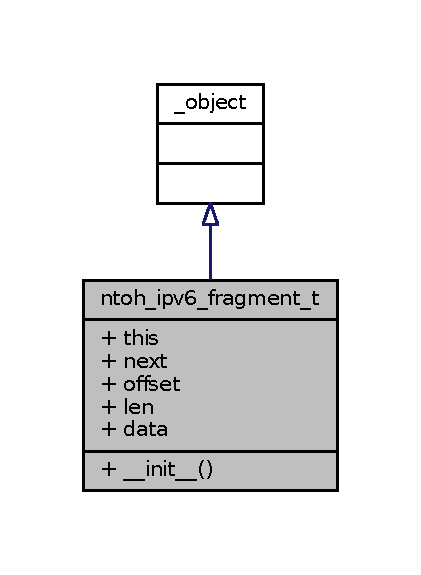
\includegraphics[width=202pt]{classlibntoh_1_1ntoh__ipv6__fragment__t__inherit__graph}
\end{center}
\end{figure}


Collaboration diagram for ntoh\-\_\-ipv6\-\_\-fragment\-\_\-t\-:
\nopagebreak
\begin{figure}[H]
\begin{center}
\leavevmode
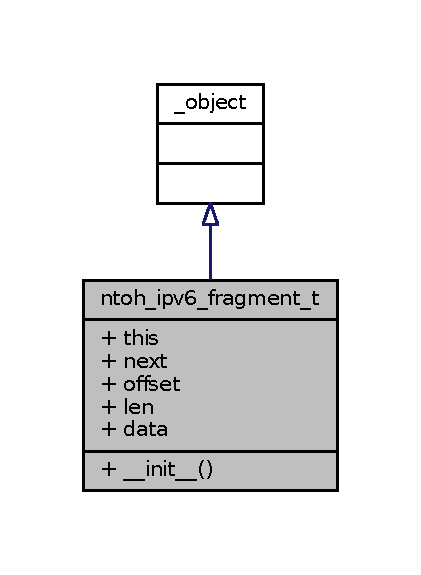
\includegraphics[width=202pt]{classlibntoh_1_1ntoh__ipv6__fragment__t__coll__graph}
\end{center}
\end{figure}
\subsection*{Public Member Functions}
\begin{DoxyCompactItemize}
\item 
def \hyperlink{classlibntoh_1_1ntoh__ipv6__fragment__t_ac775ee34451fdfa742b318538164070e}{\-\_\-\-\_\-init\-\_\-\-\_\-}
\end{DoxyCompactItemize}
\subsection*{Data Fields}
\begin{DoxyCompactItemize}
\item 
\hyperlink{classlibntoh_1_1ntoh__ipv6__fragment__t_a05c09a5e9d53fa7adf0a7936038c2fa3}{this}
\end{DoxyCompactItemize}
\subsection*{Static Public Attributes}
\begin{DoxyCompactItemize}
\item 
tuple \hyperlink{classlibntoh_1_1ntoh__ipv6__fragment__t_a84e6dac37062f5a539ece8248c8567cc}{next} = \hyperlink{namespacelibntoh_ae6f5626f776538e0cdb00e75ca1c96c9}{\-\_\-swig\-\_\-property}(\-\_\-libntoh.\-ntoh\-\_\-ipv6\-\_\-fragment\-\_\-t\-\_\-next\-\_\-get, \-\_\-libntoh.\-ntoh\-\_\-ipv6\-\_\-fragment\-\_\-t\-\_\-next\-\_\-set)
\item 
tuple \hyperlink{classlibntoh_1_1ntoh__ipv6__fragment__t_a03fbaceb13719d1bc975d26c3b92761a}{offset} = \hyperlink{namespacelibntoh_ae6f5626f776538e0cdb00e75ca1c96c9}{\-\_\-swig\-\_\-property}(\-\_\-libntoh.\-ntoh\-\_\-ipv6\-\_\-fragment\-\_\-t\-\_\-offset\-\_\-get, \-\_\-libntoh.\-ntoh\-\_\-ipv6\-\_\-fragment\-\_\-t\-\_\-offset\-\_\-set)
\item 
tuple \hyperlink{classlibntoh_1_1ntoh__ipv6__fragment__t_af8e41b97a0d8adea11037648944de58f}{len} = \hyperlink{namespacelibntoh_ae6f5626f776538e0cdb00e75ca1c96c9}{\-\_\-swig\-\_\-property}(\-\_\-libntoh.\-ntoh\-\_\-ipv6\-\_\-fragment\-\_\-t\-\_\-len\-\_\-get, \-\_\-libntoh.\-ntoh\-\_\-ipv6\-\_\-fragment\-\_\-t\-\_\-len\-\_\-set)
\item 
tuple \hyperlink{classlibntoh_1_1ntoh__ipv6__fragment__t_aa7a0efb8690a34f61a95b00cc723ca27}{data} = \hyperlink{namespacelibntoh_ae6f5626f776538e0cdb00e75ca1c96c9}{\-\_\-swig\-\_\-property}(\-\_\-libntoh.\-ntoh\-\_\-ipv6\-\_\-fragment\-\_\-t\-\_\-data\-\_\-get, \-\_\-libntoh.\-ntoh\-\_\-ipv6\-\_\-fragment\-\_\-t\-\_\-data\-\_\-set)
\end{DoxyCompactItemize}


\subsection{Constructor \& Destructor Documentation}
\hypertarget{classlibntoh_1_1ntoh__ipv6__fragment__t_ac775ee34451fdfa742b318538164070e}{\index{libntoh\-::ntoh\-\_\-ipv6\-\_\-fragment\-\_\-t@{libntoh\-::ntoh\-\_\-ipv6\-\_\-fragment\-\_\-t}!\-\_\-\-\_\-init\-\_\-\-\_\-@{\-\_\-\-\_\-init\-\_\-\-\_\-}}
\index{\-\_\-\-\_\-init\-\_\-\-\_\-@{\-\_\-\-\_\-init\-\_\-\-\_\-}!libntoh::ntoh_ipv6_fragment_t@{libntoh\-::ntoh\-\_\-ipv6\-\_\-fragment\-\_\-t}}
\subsubsection[{\-\_\-\-\_\-init\-\_\-\-\_\-}]{\setlength{\rightskip}{0pt plus 5cm}def \-\_\-\-\_\-init\-\_\-\-\_\- (
\begin{DoxyParamCaption}
\item[{}]{self}
\end{DoxyParamCaption}
)}}\label{classlibntoh_1_1ntoh__ipv6__fragment__t_ac775ee34451fdfa742b318538164070e}


\subsection{Field Documentation}
\hypertarget{classlibntoh_1_1ntoh__ipv6__fragment__t_aa7a0efb8690a34f61a95b00cc723ca27}{\index{libntoh\-::ntoh\-\_\-ipv6\-\_\-fragment\-\_\-t@{libntoh\-::ntoh\-\_\-ipv6\-\_\-fragment\-\_\-t}!data@{data}}
\index{data@{data}!libntoh::ntoh_ipv6_fragment_t@{libntoh\-::ntoh\-\_\-ipv6\-\_\-fragment\-\_\-t}}
\subsubsection[{data}]{\setlength{\rightskip}{0pt plus 5cm}tuple data = {\bf \-\_\-swig\-\_\-property}(\-\_\-libntoh.\-ntoh\-\_\-ipv6\-\_\-fragment\-\_\-t\-\_\-data\-\_\-get, \-\_\-libntoh.\-ntoh\-\_\-ipv6\-\_\-fragment\-\_\-t\-\_\-data\-\_\-set)\hspace{0.3cm}{\ttfamily [static]}}}\label{classlibntoh_1_1ntoh__ipv6__fragment__t_aa7a0efb8690a34f61a95b00cc723ca27}
\hypertarget{classlibntoh_1_1ntoh__ipv6__fragment__t_af8e41b97a0d8adea11037648944de58f}{\index{libntoh\-::ntoh\-\_\-ipv6\-\_\-fragment\-\_\-t@{libntoh\-::ntoh\-\_\-ipv6\-\_\-fragment\-\_\-t}!len@{len}}
\index{len@{len}!libntoh::ntoh_ipv6_fragment_t@{libntoh\-::ntoh\-\_\-ipv6\-\_\-fragment\-\_\-t}}
\subsubsection[{len}]{\setlength{\rightskip}{0pt plus 5cm}tuple len = {\bf \-\_\-swig\-\_\-property}(\-\_\-libntoh.\-ntoh\-\_\-ipv6\-\_\-fragment\-\_\-t\-\_\-len\-\_\-get, \-\_\-libntoh.\-ntoh\-\_\-ipv6\-\_\-fragment\-\_\-t\-\_\-len\-\_\-set)\hspace{0.3cm}{\ttfamily [static]}}}\label{classlibntoh_1_1ntoh__ipv6__fragment__t_af8e41b97a0d8adea11037648944de58f}
\hypertarget{classlibntoh_1_1ntoh__ipv6__fragment__t_a84e6dac37062f5a539ece8248c8567cc}{\index{libntoh\-::ntoh\-\_\-ipv6\-\_\-fragment\-\_\-t@{libntoh\-::ntoh\-\_\-ipv6\-\_\-fragment\-\_\-t}!next@{next}}
\index{next@{next}!libntoh::ntoh_ipv6_fragment_t@{libntoh\-::ntoh\-\_\-ipv6\-\_\-fragment\-\_\-t}}
\subsubsection[{next}]{\setlength{\rightskip}{0pt plus 5cm}tuple next = {\bf \-\_\-swig\-\_\-property}(\-\_\-libntoh.\-ntoh\-\_\-ipv6\-\_\-fragment\-\_\-t\-\_\-next\-\_\-get, \-\_\-libntoh.\-ntoh\-\_\-ipv6\-\_\-fragment\-\_\-t\-\_\-next\-\_\-set)\hspace{0.3cm}{\ttfamily [static]}}}\label{classlibntoh_1_1ntoh__ipv6__fragment__t_a84e6dac37062f5a539ece8248c8567cc}
\hypertarget{classlibntoh_1_1ntoh__ipv6__fragment__t_a03fbaceb13719d1bc975d26c3b92761a}{\index{libntoh\-::ntoh\-\_\-ipv6\-\_\-fragment\-\_\-t@{libntoh\-::ntoh\-\_\-ipv6\-\_\-fragment\-\_\-t}!offset@{offset}}
\index{offset@{offset}!libntoh::ntoh_ipv6_fragment_t@{libntoh\-::ntoh\-\_\-ipv6\-\_\-fragment\-\_\-t}}
\subsubsection[{offset}]{\setlength{\rightskip}{0pt plus 5cm}tuple offset = {\bf \-\_\-swig\-\_\-property}(\-\_\-libntoh.\-ntoh\-\_\-ipv6\-\_\-fragment\-\_\-t\-\_\-offset\-\_\-get, \-\_\-libntoh.\-ntoh\-\_\-ipv6\-\_\-fragment\-\_\-t\-\_\-offset\-\_\-set)\hspace{0.3cm}{\ttfamily [static]}}}\label{classlibntoh_1_1ntoh__ipv6__fragment__t_a03fbaceb13719d1bc975d26c3b92761a}
\hypertarget{classlibntoh_1_1ntoh__ipv6__fragment__t_a05c09a5e9d53fa7adf0a7936038c2fa3}{\index{libntoh\-::ntoh\-\_\-ipv6\-\_\-fragment\-\_\-t@{libntoh\-::ntoh\-\_\-ipv6\-\_\-fragment\-\_\-t}!this@{this}}
\index{this@{this}!libntoh::ntoh_ipv6_fragment_t@{libntoh\-::ntoh\-\_\-ipv6\-\_\-fragment\-\_\-t}}
\subsubsection[{this}]{\setlength{\rightskip}{0pt plus 5cm}this}}\label{classlibntoh_1_1ntoh__ipv6__fragment__t_a05c09a5e9d53fa7adf0a7936038c2fa3}


The documentation for this class was generated from the following file\-:\begin{DoxyCompactItemize}
\item 
build/\hyperlink{libntoh_8py}{libntoh.\-py}\end{DoxyCompactItemize}

\hypertarget{classlibntoh_1_1ntoh__ipv6__session__t}{\section{ntoh\-\_\-ipv6\-\_\-session\-\_\-t Class Reference}
\label{classlibntoh_1_1ntoh__ipv6__session__t}\index{ntoh\-\_\-ipv6\-\_\-session\-\_\-t@{ntoh\-\_\-ipv6\-\_\-session\-\_\-t}}
}


Inheritance diagram for ntoh\-\_\-ipv6\-\_\-session\-\_\-t\-:
\nopagebreak
\begin{figure}[H]
\begin{center}
\leavevmode
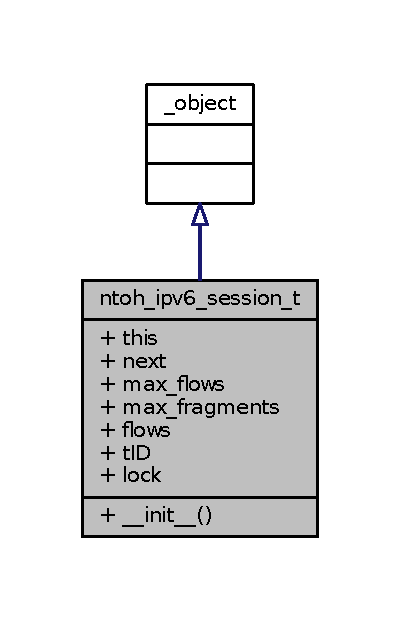
\includegraphics[width=192pt]{classlibntoh_1_1ntoh__ipv6__session__t__inherit__graph}
\end{center}
\end{figure}


Collaboration diagram for ntoh\-\_\-ipv6\-\_\-session\-\_\-t\-:
\nopagebreak
\begin{figure}[H]
\begin{center}
\leavevmode
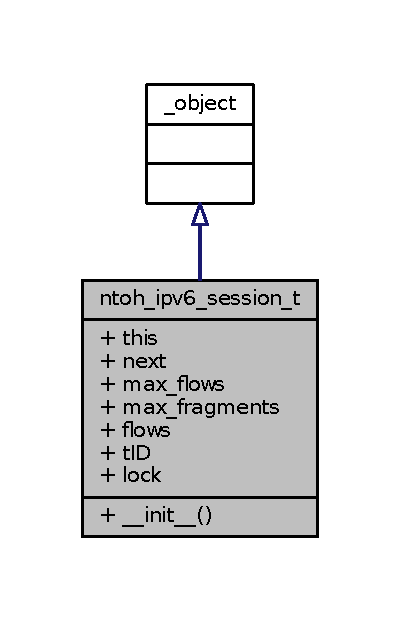
\includegraphics[width=192pt]{classlibntoh_1_1ntoh__ipv6__session__t__coll__graph}
\end{center}
\end{figure}
\subsection*{Public Member Functions}
\begin{DoxyCompactItemize}
\item 
def \hyperlink{classlibntoh_1_1ntoh__ipv6__session__t_ac775ee34451fdfa742b318538164070e}{\-\_\-\-\_\-init\-\_\-\-\_\-}
\end{DoxyCompactItemize}
\subsection*{Data Fields}
\begin{DoxyCompactItemize}
\item 
\hyperlink{classlibntoh_1_1ntoh__ipv6__session__t_a05c09a5e9d53fa7adf0a7936038c2fa3}{this}
\end{DoxyCompactItemize}
\subsection*{Static Public Attributes}
\begin{DoxyCompactItemize}
\item 
tuple \hyperlink{classlibntoh_1_1ntoh__ipv6__session__t_a84e6dac37062f5a539ece8248c8567cc}{next} = \hyperlink{namespacelibntoh_ae6f5626f776538e0cdb00e75ca1c96c9}{\-\_\-swig\-\_\-property}(\-\_\-libntoh.\-ntoh\-\_\-ipv6\-\_\-session\-\_\-t\-\_\-next\-\_\-get, \-\_\-libntoh.\-ntoh\-\_\-ipv6\-\_\-session\-\_\-t\-\_\-next\-\_\-set)
\item 
tuple \hyperlink{classlibntoh_1_1ntoh__ipv6__session__t_af05028fd588ff1bc962a8a89057a3716}{max\-\_\-flows} = \hyperlink{namespacelibntoh_ae6f5626f776538e0cdb00e75ca1c96c9}{\-\_\-swig\-\_\-property}(\-\_\-libntoh.\-ntoh\-\_\-ipv6\-\_\-session\-\_\-t\-\_\-max\-\_\-flows\-\_\-get, \-\_\-libntoh.\-ntoh\-\_\-ipv6\-\_\-session\-\_\-t\-\_\-max\-\_\-flows\-\_\-set)
\item 
tuple \hyperlink{classlibntoh_1_1ntoh__ipv6__session__t_aae26317f4443b9f0f36780fb035d1ec9}{max\-\_\-fragments} = \hyperlink{namespacelibntoh_ae6f5626f776538e0cdb00e75ca1c96c9}{\-\_\-swig\-\_\-property}(\-\_\-libntoh.\-ntoh\-\_\-ipv6\-\_\-session\-\_\-t\-\_\-max\-\_\-fragments\-\_\-get, \-\_\-libntoh.\-ntoh\-\_\-ipv6\-\_\-session\-\_\-t\-\_\-max\-\_\-fragments\-\_\-set)
\item 
tuple \hyperlink{classlibntoh_1_1ntoh__ipv6__session__t_afca3cb4196e6410df799227741f11b5e}{flows} = \hyperlink{namespacelibntoh_ae6f5626f776538e0cdb00e75ca1c96c9}{\-\_\-swig\-\_\-property}(\-\_\-libntoh.\-ntoh\-\_\-ipv6\-\_\-session\-\_\-t\-\_\-flows\-\_\-get, \-\_\-libntoh.\-ntoh\-\_\-ipv6\-\_\-session\-\_\-t\-\_\-flows\-\_\-set)
\item 
tuple \hyperlink{classlibntoh_1_1ntoh__ipv6__session__t_aa8af5c32a2a96a7fe7e14b7ebd2057ba}{t\-I\-D} = \hyperlink{namespacelibntoh_ae6f5626f776538e0cdb00e75ca1c96c9}{\-\_\-swig\-\_\-property}(\-\_\-libntoh.\-ntoh\-\_\-ipv6\-\_\-session\-\_\-t\-\_\-t\-I\-D\-\_\-get, \-\_\-libntoh.\-ntoh\-\_\-ipv6\-\_\-session\-\_\-t\-\_\-t\-I\-D\-\_\-set)
\item 
tuple \hyperlink{classlibntoh_1_1ntoh__ipv6__session__t_a871c7bf899334194698c2a3bced5e064}{lock} = \hyperlink{namespacelibntoh_ae6f5626f776538e0cdb00e75ca1c96c9}{\-\_\-swig\-\_\-property}(\-\_\-libntoh.\-ntoh\-\_\-ipv6\-\_\-session\-\_\-t\-\_\-lock\-\_\-get, \-\_\-libntoh.\-ntoh\-\_\-ipv6\-\_\-session\-\_\-t\-\_\-lock\-\_\-set)
\end{DoxyCompactItemize}


\subsection{Constructor \& Destructor Documentation}
\hypertarget{classlibntoh_1_1ntoh__ipv6__session__t_ac775ee34451fdfa742b318538164070e}{\index{libntoh\-::ntoh\-\_\-ipv6\-\_\-session\-\_\-t@{libntoh\-::ntoh\-\_\-ipv6\-\_\-session\-\_\-t}!\-\_\-\-\_\-init\-\_\-\-\_\-@{\-\_\-\-\_\-init\-\_\-\-\_\-}}
\index{\-\_\-\-\_\-init\-\_\-\-\_\-@{\-\_\-\-\_\-init\-\_\-\-\_\-}!libntoh::ntoh_ipv6_session_t@{libntoh\-::ntoh\-\_\-ipv6\-\_\-session\-\_\-t}}
\subsubsection[{\-\_\-\-\_\-init\-\_\-\-\_\-}]{\setlength{\rightskip}{0pt plus 5cm}def \-\_\-\-\_\-init\-\_\-\-\_\- (
\begin{DoxyParamCaption}
\item[{}]{self}
\end{DoxyParamCaption}
)}}\label{classlibntoh_1_1ntoh__ipv6__session__t_ac775ee34451fdfa742b318538164070e}


\subsection{Field Documentation}
\hypertarget{classlibntoh_1_1ntoh__ipv6__session__t_afca3cb4196e6410df799227741f11b5e}{\index{libntoh\-::ntoh\-\_\-ipv6\-\_\-session\-\_\-t@{libntoh\-::ntoh\-\_\-ipv6\-\_\-session\-\_\-t}!flows@{flows}}
\index{flows@{flows}!libntoh::ntoh_ipv6_session_t@{libntoh\-::ntoh\-\_\-ipv6\-\_\-session\-\_\-t}}
\subsubsection[{flows}]{\setlength{\rightskip}{0pt plus 5cm}tuple flows = {\bf \-\_\-swig\-\_\-property}(\-\_\-libntoh.\-ntoh\-\_\-ipv6\-\_\-session\-\_\-t\-\_\-flows\-\_\-get, \-\_\-libntoh.\-ntoh\-\_\-ipv6\-\_\-session\-\_\-t\-\_\-flows\-\_\-set)\hspace{0.3cm}{\ttfamily [static]}}}\label{classlibntoh_1_1ntoh__ipv6__session__t_afca3cb4196e6410df799227741f11b5e}
\hypertarget{classlibntoh_1_1ntoh__ipv6__session__t_a871c7bf899334194698c2a3bced5e064}{\index{libntoh\-::ntoh\-\_\-ipv6\-\_\-session\-\_\-t@{libntoh\-::ntoh\-\_\-ipv6\-\_\-session\-\_\-t}!lock@{lock}}
\index{lock@{lock}!libntoh::ntoh_ipv6_session_t@{libntoh\-::ntoh\-\_\-ipv6\-\_\-session\-\_\-t}}
\subsubsection[{lock}]{\setlength{\rightskip}{0pt plus 5cm}tuple lock = {\bf \-\_\-swig\-\_\-property}(\-\_\-libntoh.\-ntoh\-\_\-ipv6\-\_\-session\-\_\-t\-\_\-lock\-\_\-get, \-\_\-libntoh.\-ntoh\-\_\-ipv6\-\_\-session\-\_\-t\-\_\-lock\-\_\-set)\hspace{0.3cm}{\ttfamily [static]}}}\label{classlibntoh_1_1ntoh__ipv6__session__t_a871c7bf899334194698c2a3bced5e064}
\hypertarget{classlibntoh_1_1ntoh__ipv6__session__t_af05028fd588ff1bc962a8a89057a3716}{\index{libntoh\-::ntoh\-\_\-ipv6\-\_\-session\-\_\-t@{libntoh\-::ntoh\-\_\-ipv6\-\_\-session\-\_\-t}!max\-\_\-flows@{max\-\_\-flows}}
\index{max\-\_\-flows@{max\-\_\-flows}!libntoh::ntoh_ipv6_session_t@{libntoh\-::ntoh\-\_\-ipv6\-\_\-session\-\_\-t}}
\subsubsection[{max\-\_\-flows}]{\setlength{\rightskip}{0pt plus 5cm}tuple max\-\_\-flows = {\bf \-\_\-swig\-\_\-property}(\-\_\-libntoh.\-ntoh\-\_\-ipv6\-\_\-session\-\_\-t\-\_\-max\-\_\-flows\-\_\-get, \-\_\-libntoh.\-ntoh\-\_\-ipv6\-\_\-session\-\_\-t\-\_\-max\-\_\-flows\-\_\-set)\hspace{0.3cm}{\ttfamily [static]}}}\label{classlibntoh_1_1ntoh__ipv6__session__t_af05028fd588ff1bc962a8a89057a3716}
\hypertarget{classlibntoh_1_1ntoh__ipv6__session__t_aae26317f4443b9f0f36780fb035d1ec9}{\index{libntoh\-::ntoh\-\_\-ipv6\-\_\-session\-\_\-t@{libntoh\-::ntoh\-\_\-ipv6\-\_\-session\-\_\-t}!max\-\_\-fragments@{max\-\_\-fragments}}
\index{max\-\_\-fragments@{max\-\_\-fragments}!libntoh::ntoh_ipv6_session_t@{libntoh\-::ntoh\-\_\-ipv6\-\_\-session\-\_\-t}}
\subsubsection[{max\-\_\-fragments}]{\setlength{\rightskip}{0pt plus 5cm}tuple max\-\_\-fragments = {\bf \-\_\-swig\-\_\-property}(\-\_\-libntoh.\-ntoh\-\_\-ipv6\-\_\-session\-\_\-t\-\_\-max\-\_\-fragments\-\_\-get, \-\_\-libntoh.\-ntoh\-\_\-ipv6\-\_\-session\-\_\-t\-\_\-max\-\_\-fragments\-\_\-set)\hspace{0.3cm}{\ttfamily [static]}}}\label{classlibntoh_1_1ntoh__ipv6__session__t_aae26317f4443b9f0f36780fb035d1ec9}
\hypertarget{classlibntoh_1_1ntoh__ipv6__session__t_a84e6dac37062f5a539ece8248c8567cc}{\index{libntoh\-::ntoh\-\_\-ipv6\-\_\-session\-\_\-t@{libntoh\-::ntoh\-\_\-ipv6\-\_\-session\-\_\-t}!next@{next}}
\index{next@{next}!libntoh::ntoh_ipv6_session_t@{libntoh\-::ntoh\-\_\-ipv6\-\_\-session\-\_\-t}}
\subsubsection[{next}]{\setlength{\rightskip}{0pt plus 5cm}tuple next = {\bf \-\_\-swig\-\_\-property}(\-\_\-libntoh.\-ntoh\-\_\-ipv6\-\_\-session\-\_\-t\-\_\-next\-\_\-get, \-\_\-libntoh.\-ntoh\-\_\-ipv6\-\_\-session\-\_\-t\-\_\-next\-\_\-set)\hspace{0.3cm}{\ttfamily [static]}}}\label{classlibntoh_1_1ntoh__ipv6__session__t_a84e6dac37062f5a539ece8248c8567cc}
\hypertarget{classlibntoh_1_1ntoh__ipv6__session__t_a05c09a5e9d53fa7adf0a7936038c2fa3}{\index{libntoh\-::ntoh\-\_\-ipv6\-\_\-session\-\_\-t@{libntoh\-::ntoh\-\_\-ipv6\-\_\-session\-\_\-t}!this@{this}}
\index{this@{this}!libntoh::ntoh_ipv6_session_t@{libntoh\-::ntoh\-\_\-ipv6\-\_\-session\-\_\-t}}
\subsubsection[{this}]{\setlength{\rightskip}{0pt plus 5cm}this}}\label{classlibntoh_1_1ntoh__ipv6__session__t_a05c09a5e9d53fa7adf0a7936038c2fa3}
\hypertarget{classlibntoh_1_1ntoh__ipv6__session__t_aa8af5c32a2a96a7fe7e14b7ebd2057ba}{\index{libntoh\-::ntoh\-\_\-ipv6\-\_\-session\-\_\-t@{libntoh\-::ntoh\-\_\-ipv6\-\_\-session\-\_\-t}!t\-I\-D@{t\-I\-D}}
\index{t\-I\-D@{t\-I\-D}!libntoh::ntoh_ipv6_session_t@{libntoh\-::ntoh\-\_\-ipv6\-\_\-session\-\_\-t}}
\subsubsection[{t\-I\-D}]{\setlength{\rightskip}{0pt plus 5cm}tuple t\-I\-D = {\bf \-\_\-swig\-\_\-property}(\-\_\-libntoh.\-ntoh\-\_\-ipv6\-\_\-session\-\_\-t\-\_\-t\-I\-D\-\_\-get, \-\_\-libntoh.\-ntoh\-\_\-ipv6\-\_\-session\-\_\-t\-\_\-t\-I\-D\-\_\-set)\hspace{0.3cm}{\ttfamily [static]}}}\label{classlibntoh_1_1ntoh__ipv6__session__t_aa8af5c32a2a96a7fe7e14b7ebd2057ba}


The documentation for this class was generated from the following file\-:\begin{DoxyCompactItemize}
\item 
build/\hyperlink{libntoh_8py}{libntoh.\-py}\end{DoxyCompactItemize}

\hypertarget{structntoh__ipv6__tuple4__t}{\section{ntoh\-\_\-ipv6\-\_\-tuple4\-\_\-t Struct Reference}
\label{structntoh__ipv6__tuple4__t}\index{ntoh\-\_\-ipv6\-\_\-tuple4\-\_\-t@{ntoh\-\_\-ipv6\-\_\-tuple4\-\_\-t}}
}


Struct to generate the flow key.  




{\ttfamily \#include $<$ipv6defrag.\-h$>$}



Collaboration diagram for ntoh\-\_\-ipv6\-\_\-tuple4\-\_\-t\-:
\nopagebreak
\begin{figure}[H]
\begin{center}
\leavevmode
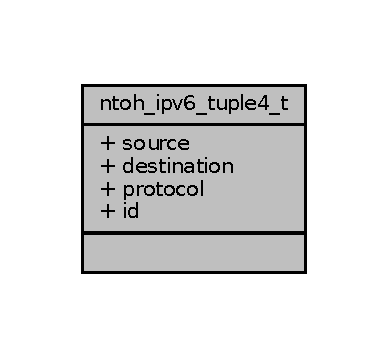
\includegraphics[width=186pt]{structntoh__ipv6__tuple4__t__coll__graph}
\end{center}
\end{figure}
\subsection*{Data Fields}
\begin{DoxyCompactItemize}
\item 
uint8\-\_\-t \hyperlink{structntoh__ipv6__tuple4__t_a6c2f6f541fb52e9338bada1c236125c1}{source} \mbox{[}16\mbox{]}
\begin{DoxyCompactList}\small\item\em source I\-P address \end{DoxyCompactList}\item 
uint8\-\_\-t \hyperlink{structntoh__ipv6__tuple4__t_a20dc0b5a2abfcfa11414f5c7f9f19111}{destination} \mbox{[}16\mbox{]}
\begin{DoxyCompactList}\small\item\em destination I\-P address \end{DoxyCompactList}\item 
uint8\-\_\-t \hyperlink{structntoh__ipv6__tuple4__t_ad124d3d2e02c729afa303c775295278e}{protocol}
\begin{DoxyCompactList}\small\item\em Transport layer protocol. \end{DoxyCompactList}\item 
unsigned int \hyperlink{structntoh__ipv6__tuple4__t_ab7ce6f462afaf105224b0ca772a33c43}{id}
\begin{DoxyCompactList}\small\item\em Identification. \end{DoxyCompactList}\end{DoxyCompactItemize}


\subsection{Detailed Description}
Struct to generate the flow key. 

\subsection{Field Documentation}
\hypertarget{structntoh__ipv6__tuple4__t_a20dc0b5a2abfcfa11414f5c7f9f19111}{\index{ntoh\-\_\-ipv6\-\_\-tuple4\-\_\-t@{ntoh\-\_\-ipv6\-\_\-tuple4\-\_\-t}!destination@{destination}}
\index{destination@{destination}!ntoh_ipv6_tuple4_t@{ntoh\-\_\-ipv6\-\_\-tuple4\-\_\-t}}
\subsubsection[{destination}]{\setlength{\rightskip}{0pt plus 5cm}uint8\-\_\-t destination\mbox{[}16\mbox{]}}}\label{structntoh__ipv6__tuple4__t_a20dc0b5a2abfcfa11414f5c7f9f19111}


destination I\-P address 

\hypertarget{structntoh__ipv6__tuple4__t_ab7ce6f462afaf105224b0ca772a33c43}{\index{ntoh\-\_\-ipv6\-\_\-tuple4\-\_\-t@{ntoh\-\_\-ipv6\-\_\-tuple4\-\_\-t}!id@{id}}
\index{id@{id}!ntoh_ipv6_tuple4_t@{ntoh\-\_\-ipv6\-\_\-tuple4\-\_\-t}}
\subsubsection[{id}]{\setlength{\rightskip}{0pt plus 5cm}unsigned int id}}\label{structntoh__ipv6__tuple4__t_ab7ce6f462afaf105224b0ca772a33c43}


Identification. 

\hypertarget{structntoh__ipv6__tuple4__t_ad124d3d2e02c729afa303c775295278e}{\index{ntoh\-\_\-ipv6\-\_\-tuple4\-\_\-t@{ntoh\-\_\-ipv6\-\_\-tuple4\-\_\-t}!protocol@{protocol}}
\index{protocol@{protocol}!ntoh_ipv6_tuple4_t@{ntoh\-\_\-ipv6\-\_\-tuple4\-\_\-t}}
\subsubsection[{protocol}]{\setlength{\rightskip}{0pt plus 5cm}uint8\-\_\-t protocol}}\label{structntoh__ipv6__tuple4__t_ad124d3d2e02c729afa303c775295278e}


Transport layer protocol. 

\hypertarget{structntoh__ipv6__tuple4__t_a6c2f6f541fb52e9338bada1c236125c1}{\index{ntoh\-\_\-ipv6\-\_\-tuple4\-\_\-t@{ntoh\-\_\-ipv6\-\_\-tuple4\-\_\-t}!source@{source}}
\index{source@{source}!ntoh_ipv6_tuple4_t@{ntoh\-\_\-ipv6\-\_\-tuple4\-\_\-t}}
\subsubsection[{source}]{\setlength{\rightskip}{0pt plus 5cm}uint8\-\_\-t source\mbox{[}16\mbox{]}}}\label{structntoh__ipv6__tuple4__t_a6c2f6f541fb52e9338bada1c236125c1}


source I\-P address 



The documentation for this struct was generated from the following file\-:\begin{DoxyCompactItemize}
\item 
inc/\hyperlink{ipv6defrag_8h}{ipv6defrag.\-h}\end{DoxyCompactItemize}

\hypertarget{classlibntoh_1_1ntoh__ipv6__tuple4__t}{\section{ntoh\-\_\-ipv6\-\_\-tuple4\-\_\-t Class Reference}
\label{classlibntoh_1_1ntoh__ipv6__tuple4__t}\index{ntoh\-\_\-ipv6\-\_\-tuple4\-\_\-t@{ntoh\-\_\-ipv6\-\_\-tuple4\-\_\-t}}
}


Inheritance diagram for ntoh\-\_\-ipv6\-\_\-tuple4\-\_\-t\-:
\nopagebreak
\begin{figure}[H]
\begin{center}
\leavevmode
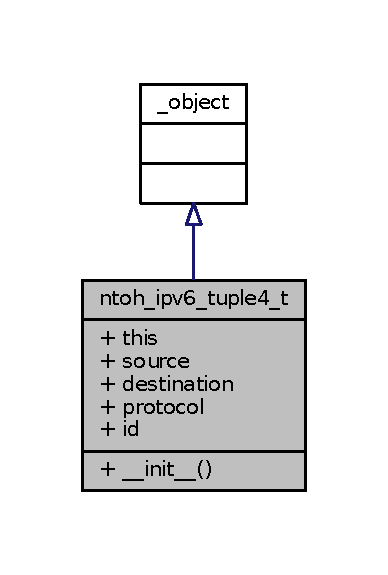
\includegraphics[width=186pt]{classlibntoh_1_1ntoh__ipv6__tuple4__t__inherit__graph}
\end{center}
\end{figure}


Collaboration diagram for ntoh\-\_\-ipv6\-\_\-tuple4\-\_\-t\-:
\nopagebreak
\begin{figure}[H]
\begin{center}
\leavevmode
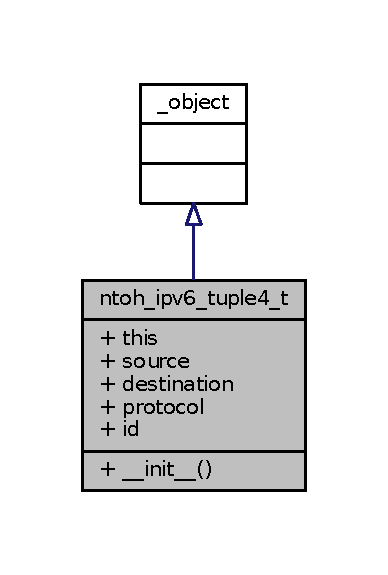
\includegraphics[width=186pt]{classlibntoh_1_1ntoh__ipv6__tuple4__t__coll__graph}
\end{center}
\end{figure}
\subsection*{Public Member Functions}
\begin{DoxyCompactItemize}
\item 
def \hyperlink{classlibntoh_1_1ntoh__ipv6__tuple4__t_ac775ee34451fdfa742b318538164070e}{\-\_\-\-\_\-init\-\_\-\-\_\-}
\end{DoxyCompactItemize}
\subsection*{Data Fields}
\begin{DoxyCompactItemize}
\item 
\hyperlink{classlibntoh_1_1ntoh__ipv6__tuple4__t_a05c09a5e9d53fa7adf0a7936038c2fa3}{this}
\end{DoxyCompactItemize}
\subsection*{Static Public Attributes}
\begin{DoxyCompactItemize}
\item 
tuple \hyperlink{classlibntoh_1_1ntoh__ipv6__tuple4__t_aa873026052cc3e5ba03877243fcb7ecd}{source} = \hyperlink{namespacelibntoh_ae6f5626f776538e0cdb00e75ca1c96c9}{\-\_\-swig\-\_\-property}(\-\_\-libntoh.\-ntoh\-\_\-ipv6\-\_\-tuple4\-\_\-t\-\_\-source\-\_\-get, \-\_\-libntoh.\-ntoh\-\_\-ipv6\-\_\-tuple4\-\_\-t\-\_\-source\-\_\-set)
\item 
tuple \hyperlink{classlibntoh_1_1ntoh__ipv6__tuple4__t_adaac82457baf1096d1c38cadf8123ce7}{destination} = \hyperlink{namespacelibntoh_ae6f5626f776538e0cdb00e75ca1c96c9}{\-\_\-swig\-\_\-property}(\-\_\-libntoh.\-ntoh\-\_\-ipv6\-\_\-tuple4\-\_\-t\-\_\-destination\-\_\-get, \-\_\-libntoh.\-ntoh\-\_\-ipv6\-\_\-tuple4\-\_\-t\-\_\-destination\-\_\-set)
\item 
tuple \hyperlink{classlibntoh_1_1ntoh__ipv6__tuple4__t_ae535ff0dd346855882bd298a9e22bbc1}{protocol} = \hyperlink{namespacelibntoh_ae6f5626f776538e0cdb00e75ca1c96c9}{\-\_\-swig\-\_\-property}(\-\_\-libntoh.\-ntoh\-\_\-ipv6\-\_\-tuple4\-\_\-t\-\_\-protocol\-\_\-get, \-\_\-libntoh.\-ntoh\-\_\-ipv6\-\_\-tuple4\-\_\-t\-\_\-protocol\-\_\-set)
\item 
tuple \hyperlink{classlibntoh_1_1ntoh__ipv6__tuple4__t_a0e43f6071072440917ee2dd8af07d251}{id} = \hyperlink{namespacelibntoh_ae6f5626f776538e0cdb00e75ca1c96c9}{\-\_\-swig\-\_\-property}(\-\_\-libntoh.\-ntoh\-\_\-ipv6\-\_\-tuple4\-\_\-t\-\_\-id\-\_\-get, \-\_\-libntoh.\-ntoh\-\_\-ipv6\-\_\-tuple4\-\_\-t\-\_\-id\-\_\-set)
\end{DoxyCompactItemize}


\subsection{Constructor \& Destructor Documentation}
\hypertarget{classlibntoh_1_1ntoh__ipv6__tuple4__t_ac775ee34451fdfa742b318538164070e}{\index{libntoh\-::ntoh\-\_\-ipv6\-\_\-tuple4\-\_\-t@{libntoh\-::ntoh\-\_\-ipv6\-\_\-tuple4\-\_\-t}!\-\_\-\-\_\-init\-\_\-\-\_\-@{\-\_\-\-\_\-init\-\_\-\-\_\-}}
\index{\-\_\-\-\_\-init\-\_\-\-\_\-@{\-\_\-\-\_\-init\-\_\-\-\_\-}!libntoh::ntoh_ipv6_tuple4_t@{libntoh\-::ntoh\-\_\-ipv6\-\_\-tuple4\-\_\-t}}
\subsubsection[{\-\_\-\-\_\-init\-\_\-\-\_\-}]{\setlength{\rightskip}{0pt plus 5cm}def \-\_\-\-\_\-init\-\_\-\-\_\- (
\begin{DoxyParamCaption}
\item[{}]{self}
\end{DoxyParamCaption}
)}}\label{classlibntoh_1_1ntoh__ipv6__tuple4__t_ac775ee34451fdfa742b318538164070e}


\subsection{Field Documentation}
\hypertarget{classlibntoh_1_1ntoh__ipv6__tuple4__t_adaac82457baf1096d1c38cadf8123ce7}{\index{libntoh\-::ntoh\-\_\-ipv6\-\_\-tuple4\-\_\-t@{libntoh\-::ntoh\-\_\-ipv6\-\_\-tuple4\-\_\-t}!destination@{destination}}
\index{destination@{destination}!libntoh::ntoh_ipv6_tuple4_t@{libntoh\-::ntoh\-\_\-ipv6\-\_\-tuple4\-\_\-t}}
\subsubsection[{destination}]{\setlength{\rightskip}{0pt plus 5cm}tuple destination = {\bf \-\_\-swig\-\_\-property}(\-\_\-libntoh.\-ntoh\-\_\-ipv6\-\_\-tuple4\-\_\-t\-\_\-destination\-\_\-get, \-\_\-libntoh.\-ntoh\-\_\-ipv6\-\_\-tuple4\-\_\-t\-\_\-destination\-\_\-set)\hspace{0.3cm}{\ttfamily [static]}}}\label{classlibntoh_1_1ntoh__ipv6__tuple4__t_adaac82457baf1096d1c38cadf8123ce7}
\hypertarget{classlibntoh_1_1ntoh__ipv6__tuple4__t_a0e43f6071072440917ee2dd8af07d251}{\index{libntoh\-::ntoh\-\_\-ipv6\-\_\-tuple4\-\_\-t@{libntoh\-::ntoh\-\_\-ipv6\-\_\-tuple4\-\_\-t}!id@{id}}
\index{id@{id}!libntoh::ntoh_ipv6_tuple4_t@{libntoh\-::ntoh\-\_\-ipv6\-\_\-tuple4\-\_\-t}}
\subsubsection[{id}]{\setlength{\rightskip}{0pt plus 5cm}tuple id = {\bf \-\_\-swig\-\_\-property}(\-\_\-libntoh.\-ntoh\-\_\-ipv6\-\_\-tuple4\-\_\-t\-\_\-id\-\_\-get, \-\_\-libntoh.\-ntoh\-\_\-ipv6\-\_\-tuple4\-\_\-t\-\_\-id\-\_\-set)\hspace{0.3cm}{\ttfamily [static]}}}\label{classlibntoh_1_1ntoh__ipv6__tuple4__t_a0e43f6071072440917ee2dd8af07d251}
\hypertarget{classlibntoh_1_1ntoh__ipv6__tuple4__t_ae535ff0dd346855882bd298a9e22bbc1}{\index{libntoh\-::ntoh\-\_\-ipv6\-\_\-tuple4\-\_\-t@{libntoh\-::ntoh\-\_\-ipv6\-\_\-tuple4\-\_\-t}!protocol@{protocol}}
\index{protocol@{protocol}!libntoh::ntoh_ipv6_tuple4_t@{libntoh\-::ntoh\-\_\-ipv6\-\_\-tuple4\-\_\-t}}
\subsubsection[{protocol}]{\setlength{\rightskip}{0pt plus 5cm}tuple protocol = {\bf \-\_\-swig\-\_\-property}(\-\_\-libntoh.\-ntoh\-\_\-ipv6\-\_\-tuple4\-\_\-t\-\_\-protocol\-\_\-get, \-\_\-libntoh.\-ntoh\-\_\-ipv6\-\_\-tuple4\-\_\-t\-\_\-protocol\-\_\-set)\hspace{0.3cm}{\ttfamily [static]}}}\label{classlibntoh_1_1ntoh__ipv6__tuple4__t_ae535ff0dd346855882bd298a9e22bbc1}
\hypertarget{classlibntoh_1_1ntoh__ipv6__tuple4__t_aa873026052cc3e5ba03877243fcb7ecd}{\index{libntoh\-::ntoh\-\_\-ipv6\-\_\-tuple4\-\_\-t@{libntoh\-::ntoh\-\_\-ipv6\-\_\-tuple4\-\_\-t}!source@{source}}
\index{source@{source}!libntoh::ntoh_ipv6_tuple4_t@{libntoh\-::ntoh\-\_\-ipv6\-\_\-tuple4\-\_\-t}}
\subsubsection[{source}]{\setlength{\rightskip}{0pt plus 5cm}tuple source = {\bf \-\_\-swig\-\_\-property}(\-\_\-libntoh.\-ntoh\-\_\-ipv6\-\_\-tuple4\-\_\-t\-\_\-source\-\_\-get, \-\_\-libntoh.\-ntoh\-\_\-ipv6\-\_\-tuple4\-\_\-t\-\_\-source\-\_\-set)\hspace{0.3cm}{\ttfamily [static]}}}\label{classlibntoh_1_1ntoh__ipv6__tuple4__t_aa873026052cc3e5ba03877243fcb7ecd}
\hypertarget{classlibntoh_1_1ntoh__ipv6__tuple4__t_a05c09a5e9d53fa7adf0a7936038c2fa3}{\index{libntoh\-::ntoh\-\_\-ipv6\-\_\-tuple4\-\_\-t@{libntoh\-::ntoh\-\_\-ipv6\-\_\-tuple4\-\_\-t}!this@{this}}
\index{this@{this}!libntoh::ntoh_ipv6_tuple4_t@{libntoh\-::ntoh\-\_\-ipv6\-\_\-tuple4\-\_\-t}}
\subsubsection[{this}]{\setlength{\rightskip}{0pt plus 5cm}this}}\label{classlibntoh_1_1ntoh__ipv6__tuple4__t_a05c09a5e9d53fa7adf0a7936038c2fa3}


The documentation for this class was generated from the following file\-:\begin{DoxyCompactItemize}
\item 
build/\hyperlink{libntoh_8py}{libntoh.\-py}\end{DoxyCompactItemize}

\hypertarget{classlibntoh_1_1ntoh__lock__t}{\section{ntoh\-\_\-lock\-\_\-t Class Reference}
\label{classlibntoh_1_1ntoh__lock__t}\index{ntoh\-\_\-lock\-\_\-t@{ntoh\-\_\-lock\-\_\-t}}
}


Inheritance diagram for ntoh\-\_\-lock\-\_\-t\-:
\nopagebreak
\begin{figure}[H]
\begin{center}
\leavevmode
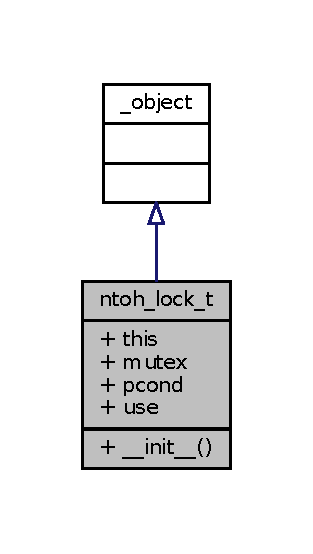
\includegraphics[width=150pt]{classlibntoh_1_1ntoh__lock__t__inherit__graph}
\end{center}
\end{figure}


Collaboration diagram for ntoh\-\_\-lock\-\_\-t\-:
\nopagebreak
\begin{figure}[H]
\begin{center}
\leavevmode
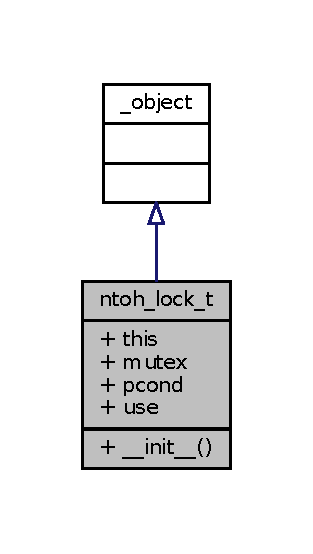
\includegraphics[width=150pt]{classlibntoh_1_1ntoh__lock__t__coll__graph}
\end{center}
\end{figure}
\subsection*{Public Member Functions}
\begin{DoxyCompactItemize}
\item 
def \hyperlink{classlibntoh_1_1ntoh__lock__t_ac775ee34451fdfa742b318538164070e}{\-\_\-\-\_\-init\-\_\-\-\_\-}
\end{DoxyCompactItemize}
\subsection*{Data Fields}
\begin{DoxyCompactItemize}
\item 
\hyperlink{classlibntoh_1_1ntoh__lock__t_a05c09a5e9d53fa7adf0a7936038c2fa3}{this}
\end{DoxyCompactItemize}
\subsection*{Static Public Attributes}
\begin{DoxyCompactItemize}
\item 
tuple \hyperlink{classlibntoh_1_1ntoh__lock__t_a8f7d48b1501f5673c6742b61e778ce01}{mutex} = \hyperlink{namespacelibntoh_ae6f5626f776538e0cdb00e75ca1c96c9}{\-\_\-swig\-\_\-property}(\-\_\-libntoh.\-ntoh\-\_\-lock\-\_\-t\-\_\-mutex\-\_\-get, \-\_\-libntoh.\-ntoh\-\_\-lock\-\_\-t\-\_\-mutex\-\_\-set)
\item 
tuple \hyperlink{classlibntoh_1_1ntoh__lock__t_a23a951c27c097e73988ca76b59fd56c2}{pcond} = \hyperlink{namespacelibntoh_ae6f5626f776538e0cdb00e75ca1c96c9}{\-\_\-swig\-\_\-property}(\-\_\-libntoh.\-ntoh\-\_\-lock\-\_\-t\-\_\-pcond\-\_\-get, \-\_\-libntoh.\-ntoh\-\_\-lock\-\_\-t\-\_\-pcond\-\_\-set)
\item 
tuple \hyperlink{classlibntoh_1_1ntoh__lock__t_a8f0e3ca01e3f2f394c20647dcc7abd23}{use} = \hyperlink{namespacelibntoh_ae6f5626f776538e0cdb00e75ca1c96c9}{\-\_\-swig\-\_\-property}(\-\_\-libntoh.\-ntoh\-\_\-lock\-\_\-t\-\_\-use\-\_\-get, \-\_\-libntoh.\-ntoh\-\_\-lock\-\_\-t\-\_\-use\-\_\-set)
\end{DoxyCompactItemize}


\subsection{Constructor \& Destructor Documentation}
\hypertarget{classlibntoh_1_1ntoh__lock__t_ac775ee34451fdfa742b318538164070e}{\index{libntoh\-::ntoh\-\_\-lock\-\_\-t@{libntoh\-::ntoh\-\_\-lock\-\_\-t}!\-\_\-\-\_\-init\-\_\-\-\_\-@{\-\_\-\-\_\-init\-\_\-\-\_\-}}
\index{\-\_\-\-\_\-init\-\_\-\-\_\-@{\-\_\-\-\_\-init\-\_\-\-\_\-}!libntoh::ntoh_lock_t@{libntoh\-::ntoh\-\_\-lock\-\_\-t}}
\subsubsection[{\-\_\-\-\_\-init\-\_\-\-\_\-}]{\setlength{\rightskip}{0pt plus 5cm}def \-\_\-\-\_\-init\-\_\-\-\_\- (
\begin{DoxyParamCaption}
\item[{}]{self}
\end{DoxyParamCaption}
)}}\label{classlibntoh_1_1ntoh__lock__t_ac775ee34451fdfa742b318538164070e}


\subsection{Field Documentation}
\hypertarget{classlibntoh_1_1ntoh__lock__t_a8f7d48b1501f5673c6742b61e778ce01}{\index{libntoh\-::ntoh\-\_\-lock\-\_\-t@{libntoh\-::ntoh\-\_\-lock\-\_\-t}!mutex@{mutex}}
\index{mutex@{mutex}!libntoh::ntoh_lock_t@{libntoh\-::ntoh\-\_\-lock\-\_\-t}}
\subsubsection[{mutex}]{\setlength{\rightskip}{0pt plus 5cm}tuple mutex = {\bf \-\_\-swig\-\_\-property}(\-\_\-libntoh.\-ntoh\-\_\-lock\-\_\-t\-\_\-mutex\-\_\-get, \-\_\-libntoh.\-ntoh\-\_\-lock\-\_\-t\-\_\-mutex\-\_\-set)\hspace{0.3cm}{\ttfamily [static]}}}\label{classlibntoh_1_1ntoh__lock__t_a8f7d48b1501f5673c6742b61e778ce01}
\hypertarget{classlibntoh_1_1ntoh__lock__t_a23a951c27c097e73988ca76b59fd56c2}{\index{libntoh\-::ntoh\-\_\-lock\-\_\-t@{libntoh\-::ntoh\-\_\-lock\-\_\-t}!pcond@{pcond}}
\index{pcond@{pcond}!libntoh::ntoh_lock_t@{libntoh\-::ntoh\-\_\-lock\-\_\-t}}
\subsubsection[{pcond}]{\setlength{\rightskip}{0pt plus 5cm}tuple pcond = {\bf \-\_\-swig\-\_\-property}(\-\_\-libntoh.\-ntoh\-\_\-lock\-\_\-t\-\_\-pcond\-\_\-get, \-\_\-libntoh.\-ntoh\-\_\-lock\-\_\-t\-\_\-pcond\-\_\-set)\hspace{0.3cm}{\ttfamily [static]}}}\label{classlibntoh_1_1ntoh__lock__t_a23a951c27c097e73988ca76b59fd56c2}
\hypertarget{classlibntoh_1_1ntoh__lock__t_a05c09a5e9d53fa7adf0a7936038c2fa3}{\index{libntoh\-::ntoh\-\_\-lock\-\_\-t@{libntoh\-::ntoh\-\_\-lock\-\_\-t}!this@{this}}
\index{this@{this}!libntoh::ntoh_lock_t@{libntoh\-::ntoh\-\_\-lock\-\_\-t}}
\subsubsection[{this}]{\setlength{\rightskip}{0pt plus 5cm}this}}\label{classlibntoh_1_1ntoh__lock__t_a05c09a5e9d53fa7adf0a7936038c2fa3}
\hypertarget{classlibntoh_1_1ntoh__lock__t_a8f0e3ca01e3f2f394c20647dcc7abd23}{\index{libntoh\-::ntoh\-\_\-lock\-\_\-t@{libntoh\-::ntoh\-\_\-lock\-\_\-t}!use@{use}}
\index{use@{use}!libntoh::ntoh_lock_t@{libntoh\-::ntoh\-\_\-lock\-\_\-t}}
\subsubsection[{use}]{\setlength{\rightskip}{0pt plus 5cm}tuple use = {\bf \-\_\-swig\-\_\-property}(\-\_\-libntoh.\-ntoh\-\_\-lock\-\_\-t\-\_\-use\-\_\-get, \-\_\-libntoh.\-ntoh\-\_\-lock\-\_\-t\-\_\-use\-\_\-set)\hspace{0.3cm}{\ttfamily [static]}}}\label{classlibntoh_1_1ntoh__lock__t_a8f0e3ca01e3f2f394c20647dcc7abd23}


The documentation for this class was generated from the following file\-:\begin{DoxyCompactItemize}
\item 
build/\hyperlink{libntoh_8py}{libntoh.\-py}\end{DoxyCompactItemize}

\hypertarget{structntoh__lock__t}{\section{ntoh\-\_\-lock\-\_\-t Struct Reference}
\label{structntoh__lock__t}\index{ntoh\-\_\-lock\-\_\-t@{ntoh\-\_\-lock\-\_\-t}}
}


{\ttfamily \#include $<$libntoh.\-h$>$}



Collaboration diagram for ntoh\-\_\-lock\-\_\-t\-:
\nopagebreak
\begin{figure}[H]
\begin{center}
\leavevmode
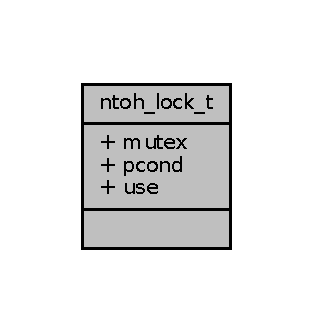
\includegraphics[width=150pt]{structntoh__lock__t__coll__graph}
\end{center}
\end{figure}
\subsection*{Data Fields}
\begin{DoxyCompactItemize}
\item 
pthread\-\_\-mutex\-\_\-t \hyperlink{structntoh__lock__t_a4acff8232e4aec9cd5c6dc200ac55ef3}{mutex}
\item 
pthread\-\_\-cond\-\_\-t \hyperlink{structntoh__lock__t_ae7a6f0d43d482747235ce5732dfd16eb}{pcond}
\item 
int \hyperlink{structntoh__lock__t_a7fa111673285c27a59c5ef465c1ab63b}{use}
\end{DoxyCompactItemize}


\subsection{Field Documentation}
\hypertarget{structntoh__lock__t_a4acff8232e4aec9cd5c6dc200ac55ef3}{\index{ntoh\-\_\-lock\-\_\-t@{ntoh\-\_\-lock\-\_\-t}!mutex@{mutex}}
\index{mutex@{mutex}!ntoh_lock_t@{ntoh\-\_\-lock\-\_\-t}}
\subsubsection[{mutex}]{\setlength{\rightskip}{0pt plus 5cm}pthread\-\_\-mutex\-\_\-t mutex}}\label{structntoh__lock__t_a4acff8232e4aec9cd5c6dc200ac55ef3}
\hypertarget{structntoh__lock__t_ae7a6f0d43d482747235ce5732dfd16eb}{\index{ntoh\-\_\-lock\-\_\-t@{ntoh\-\_\-lock\-\_\-t}!pcond@{pcond}}
\index{pcond@{pcond}!ntoh_lock_t@{ntoh\-\_\-lock\-\_\-t}}
\subsubsection[{pcond}]{\setlength{\rightskip}{0pt plus 5cm}pthread\-\_\-cond\-\_\-t pcond}}\label{structntoh__lock__t_ae7a6f0d43d482747235ce5732dfd16eb}
\hypertarget{structntoh__lock__t_a7fa111673285c27a59c5ef465c1ab63b}{\index{ntoh\-\_\-lock\-\_\-t@{ntoh\-\_\-lock\-\_\-t}!use@{use}}
\index{use@{use}!ntoh_lock_t@{ntoh\-\_\-lock\-\_\-t}}
\subsubsection[{use}]{\setlength{\rightskip}{0pt plus 5cm}int use}}\label{structntoh__lock__t_a7fa111673285c27a59c5ef465c1ab63b}


The documentation for this struct was generated from the following file\-:\begin{DoxyCompactItemize}
\item 
inc/\hyperlink{libntoh_8h}{libntoh.\-h}\end{DoxyCompactItemize}

\hypertarget{structntoh__tcp__peer__t}{\section{ntoh\-\_\-tcp\-\_\-peer\-\_\-t Struct Reference}
\label{structntoh__tcp__peer__t}\index{ntoh\-\_\-tcp\-\_\-peer\-\_\-t@{ntoh\-\_\-tcp\-\_\-peer\-\_\-t}}
}


peer information  




{\ttfamily \#include $<$tcpreassembly.\-h$>$}



Collaboration diagram for ntoh\-\_\-tcp\-\_\-peer\-\_\-t\-:
\nopagebreak
\begin{figure}[H]
\begin{center}
\leavevmode
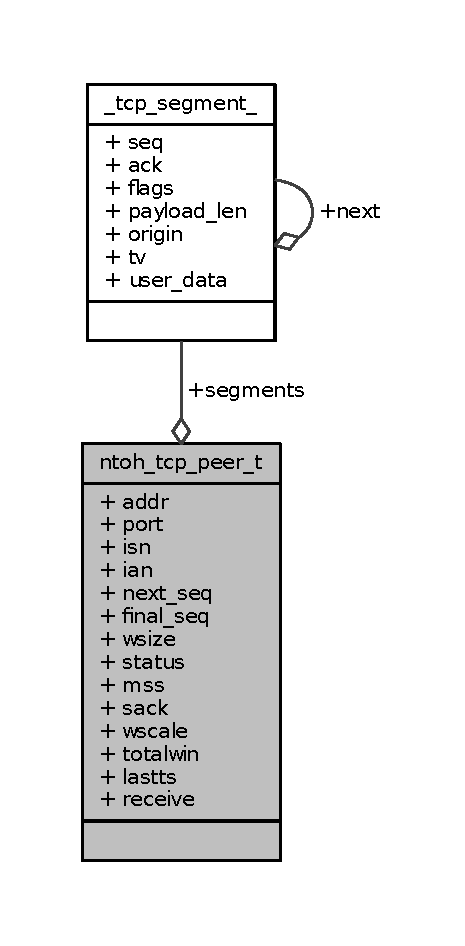
\includegraphics[width=223pt]{structntoh__tcp__peer__t__coll__graph}
\end{center}
\end{figure}
\subsection*{Data Fields}
\begin{DoxyCompactItemize}
\item 
unsigned int \hyperlink{structntoh__tcp__peer__t_ab36863a07751ac73459d46b677c33b57}{addr}
\begin{DoxyCompactList}\small\item\em I\-P address. \end{DoxyCompactList}\item 
unsigned short \hyperlink{structntoh__tcp__peer__t_ab85ff85aa1f60f4a1c1ca1225a9dad06}{port}
\begin{DoxyCompactList}\small\item\em connection port \end{DoxyCompactList}\item 
unsigned long \hyperlink{structntoh__tcp__peer__t_a9e6dafb622805bf2612b302c10f18ba5}{isn}
\begin{DoxyCompactList}\small\item\em initial S\-E\-Q. number \end{DoxyCompactList}\item 
unsigned long \hyperlink{structntoh__tcp__peer__t_acfab4beb8833b2e45a3d02b1b8eb2ae3}{ian}
\begin{DoxyCompactList}\small\item\em initial A\-C\-K. number \end{DoxyCompactList}\item 
unsigned long \hyperlink{structntoh__tcp__peer__t_a8293c38954155f30a30958c8e8100f0b}{next\-\_\-seq}
\begin{DoxyCompactList}\small\item\em N\-E\-X\-T S\-E\-Q. number. \end{DoxyCompactList}\item 
unsigned long \hyperlink{structntoh__tcp__peer__t_a9ed11c1f20c424d3a4edf704ecf07d93}{final\-\_\-seq}
\begin{DoxyCompactList}\small\item\em T\-H\-\_\-\-F\-I\-N $\vert$ T\-H\-\_\-\-R\-S\-T sequence. \end{DoxyCompactList}\item 
unsigned int \hyperlink{structntoh__tcp__peer__t_a2e4250265d88bafcbc4bdad73639c2a7}{wsize}
\begin{DoxyCompactList}\small\item\em T\-C\-P window size. \end{DoxyCompactList}\item 
unsigned int \hyperlink{structntoh__tcp__peer__t_aeed08ea57af6f7be240e2bf66162389f}{status}
\begin{DoxyCompactList}\small\item\em peer status \end{DoxyCompactList}\item 
\hyperlink{tcpreassembly_8h_a1f60f4065e8694dbf82c9896925295b3}{pntoh\-\_\-tcp\-\_\-segment\-\_\-t} \hyperlink{structntoh__tcp__peer__t_ade44d6ced1b5a51caac1af66150b610c}{segments}
\begin{DoxyCompactList}\small\item\em segments list \end{DoxyCompactList}\item 
unsigned int \hyperlink{structntoh__tcp__peer__t_a71381dd15a96b081986e0c98e1e75f90}{mss}
\begin{DoxyCompactList}\small\item\em Max. Segment Size. \end{DoxyCompactList}\item 
unsigned int \hyperlink{structntoh__tcp__peer__t_a083c3c3c4c7eb53663cd15317b55872b}{sack}
\begin{DoxyCompactList}\small\item\em Selective A\-C\-K. \end{DoxyCompactList}\item 
unsigned int \hyperlink{structntoh__tcp__peer__t_a648feb18271d5c1fe600c6bf7875478c}{wscale}
\begin{DoxyCompactList}\small\item\em window scale factor \end{DoxyCompactList}\item 
unsigned long \hyperlink{structntoh__tcp__peer__t_af40364d83cae85562184a8bee797ae6c}{totalwin}
\begin{DoxyCompactList}\small\item\em total window size \end{DoxyCompactList}\item 
unsigned int \hyperlink{structntoh__tcp__peer__t_a2eb3b9494c999b0dd38c4d40bfdc55b4}{lastts}
\begin{DoxyCompactList}\small\item\em last ts \end{DoxyCompactList}\item 
unsigned short \hyperlink{structntoh__tcp__peer__t_a51b032f0cfd74b0bdbcf8294f1f7d7b7}{receive}
\begin{DoxyCompactList}\small\item\em send peer segments to user? \end{DoxyCompactList}\end{DoxyCompactItemize}


\subsection{Detailed Description}
peer information 

\subsection{Field Documentation}
\hypertarget{structntoh__tcp__peer__t_ab36863a07751ac73459d46b677c33b57}{\index{ntoh\-\_\-tcp\-\_\-peer\-\_\-t@{ntoh\-\_\-tcp\-\_\-peer\-\_\-t}!addr@{addr}}
\index{addr@{addr}!ntoh_tcp_peer_t@{ntoh\-\_\-tcp\-\_\-peer\-\_\-t}}
\subsubsection[{addr}]{\setlength{\rightskip}{0pt plus 5cm}unsigned int addr}}\label{structntoh__tcp__peer__t_ab36863a07751ac73459d46b677c33b57}


I\-P address. 

\hypertarget{structntoh__tcp__peer__t_a9ed11c1f20c424d3a4edf704ecf07d93}{\index{ntoh\-\_\-tcp\-\_\-peer\-\_\-t@{ntoh\-\_\-tcp\-\_\-peer\-\_\-t}!final\-\_\-seq@{final\-\_\-seq}}
\index{final\-\_\-seq@{final\-\_\-seq}!ntoh_tcp_peer_t@{ntoh\-\_\-tcp\-\_\-peer\-\_\-t}}
\subsubsection[{final\-\_\-seq}]{\setlength{\rightskip}{0pt plus 5cm}unsigned long final\-\_\-seq}}\label{structntoh__tcp__peer__t_a9ed11c1f20c424d3a4edf704ecf07d93}


T\-H\-\_\-\-F\-I\-N $\vert$ T\-H\-\_\-\-R\-S\-T sequence. 

\hypertarget{structntoh__tcp__peer__t_acfab4beb8833b2e45a3d02b1b8eb2ae3}{\index{ntoh\-\_\-tcp\-\_\-peer\-\_\-t@{ntoh\-\_\-tcp\-\_\-peer\-\_\-t}!ian@{ian}}
\index{ian@{ian}!ntoh_tcp_peer_t@{ntoh\-\_\-tcp\-\_\-peer\-\_\-t}}
\subsubsection[{ian}]{\setlength{\rightskip}{0pt plus 5cm}unsigned long ian}}\label{structntoh__tcp__peer__t_acfab4beb8833b2e45a3d02b1b8eb2ae3}


initial A\-C\-K. number 

\hypertarget{structntoh__tcp__peer__t_a9e6dafb622805bf2612b302c10f18ba5}{\index{ntoh\-\_\-tcp\-\_\-peer\-\_\-t@{ntoh\-\_\-tcp\-\_\-peer\-\_\-t}!isn@{isn}}
\index{isn@{isn}!ntoh_tcp_peer_t@{ntoh\-\_\-tcp\-\_\-peer\-\_\-t}}
\subsubsection[{isn}]{\setlength{\rightskip}{0pt plus 5cm}unsigned long isn}}\label{structntoh__tcp__peer__t_a9e6dafb622805bf2612b302c10f18ba5}


initial S\-E\-Q. number 

\hypertarget{structntoh__tcp__peer__t_a2eb3b9494c999b0dd38c4d40bfdc55b4}{\index{ntoh\-\_\-tcp\-\_\-peer\-\_\-t@{ntoh\-\_\-tcp\-\_\-peer\-\_\-t}!lastts@{lastts}}
\index{lastts@{lastts}!ntoh_tcp_peer_t@{ntoh\-\_\-tcp\-\_\-peer\-\_\-t}}
\subsubsection[{lastts}]{\setlength{\rightskip}{0pt plus 5cm}unsigned int lastts}}\label{structntoh__tcp__peer__t_a2eb3b9494c999b0dd38c4d40bfdc55b4}


last ts 

\hypertarget{structntoh__tcp__peer__t_a71381dd15a96b081986e0c98e1e75f90}{\index{ntoh\-\_\-tcp\-\_\-peer\-\_\-t@{ntoh\-\_\-tcp\-\_\-peer\-\_\-t}!mss@{mss}}
\index{mss@{mss}!ntoh_tcp_peer_t@{ntoh\-\_\-tcp\-\_\-peer\-\_\-t}}
\subsubsection[{mss}]{\setlength{\rightskip}{0pt plus 5cm}unsigned int mss}}\label{structntoh__tcp__peer__t_a71381dd15a96b081986e0c98e1e75f90}


Max. Segment Size. 

\hypertarget{structntoh__tcp__peer__t_a8293c38954155f30a30958c8e8100f0b}{\index{ntoh\-\_\-tcp\-\_\-peer\-\_\-t@{ntoh\-\_\-tcp\-\_\-peer\-\_\-t}!next\-\_\-seq@{next\-\_\-seq}}
\index{next\-\_\-seq@{next\-\_\-seq}!ntoh_tcp_peer_t@{ntoh\-\_\-tcp\-\_\-peer\-\_\-t}}
\subsubsection[{next\-\_\-seq}]{\setlength{\rightskip}{0pt plus 5cm}unsigned long next\-\_\-seq}}\label{structntoh__tcp__peer__t_a8293c38954155f30a30958c8e8100f0b}


N\-E\-X\-T S\-E\-Q. number. 

\hypertarget{structntoh__tcp__peer__t_ab85ff85aa1f60f4a1c1ca1225a9dad06}{\index{ntoh\-\_\-tcp\-\_\-peer\-\_\-t@{ntoh\-\_\-tcp\-\_\-peer\-\_\-t}!port@{port}}
\index{port@{port}!ntoh_tcp_peer_t@{ntoh\-\_\-tcp\-\_\-peer\-\_\-t}}
\subsubsection[{port}]{\setlength{\rightskip}{0pt plus 5cm}unsigned short port}}\label{structntoh__tcp__peer__t_ab85ff85aa1f60f4a1c1ca1225a9dad06}


connection port 

\hypertarget{structntoh__tcp__peer__t_a51b032f0cfd74b0bdbcf8294f1f7d7b7}{\index{ntoh\-\_\-tcp\-\_\-peer\-\_\-t@{ntoh\-\_\-tcp\-\_\-peer\-\_\-t}!receive@{receive}}
\index{receive@{receive}!ntoh_tcp_peer_t@{ntoh\-\_\-tcp\-\_\-peer\-\_\-t}}
\subsubsection[{receive}]{\setlength{\rightskip}{0pt plus 5cm}unsigned short receive}}\label{structntoh__tcp__peer__t_a51b032f0cfd74b0bdbcf8294f1f7d7b7}


send peer segments to user? 

\hypertarget{structntoh__tcp__peer__t_a083c3c3c4c7eb53663cd15317b55872b}{\index{ntoh\-\_\-tcp\-\_\-peer\-\_\-t@{ntoh\-\_\-tcp\-\_\-peer\-\_\-t}!sack@{sack}}
\index{sack@{sack}!ntoh_tcp_peer_t@{ntoh\-\_\-tcp\-\_\-peer\-\_\-t}}
\subsubsection[{sack}]{\setlength{\rightskip}{0pt plus 5cm}unsigned int sack}}\label{structntoh__tcp__peer__t_a083c3c3c4c7eb53663cd15317b55872b}


Selective A\-C\-K. 

\hypertarget{structntoh__tcp__peer__t_ade44d6ced1b5a51caac1af66150b610c}{\index{ntoh\-\_\-tcp\-\_\-peer\-\_\-t@{ntoh\-\_\-tcp\-\_\-peer\-\_\-t}!segments@{segments}}
\index{segments@{segments}!ntoh_tcp_peer_t@{ntoh\-\_\-tcp\-\_\-peer\-\_\-t}}
\subsubsection[{segments}]{\setlength{\rightskip}{0pt plus 5cm}{\bf pntoh\-\_\-tcp\-\_\-segment\-\_\-t} segments}}\label{structntoh__tcp__peer__t_ade44d6ced1b5a51caac1af66150b610c}


segments list 

\hypertarget{structntoh__tcp__peer__t_aeed08ea57af6f7be240e2bf66162389f}{\index{ntoh\-\_\-tcp\-\_\-peer\-\_\-t@{ntoh\-\_\-tcp\-\_\-peer\-\_\-t}!status@{status}}
\index{status@{status}!ntoh_tcp_peer_t@{ntoh\-\_\-tcp\-\_\-peer\-\_\-t}}
\subsubsection[{status}]{\setlength{\rightskip}{0pt plus 5cm}unsigned int status}}\label{structntoh__tcp__peer__t_aeed08ea57af6f7be240e2bf66162389f}


peer status 

\hypertarget{structntoh__tcp__peer__t_af40364d83cae85562184a8bee797ae6c}{\index{ntoh\-\_\-tcp\-\_\-peer\-\_\-t@{ntoh\-\_\-tcp\-\_\-peer\-\_\-t}!totalwin@{totalwin}}
\index{totalwin@{totalwin}!ntoh_tcp_peer_t@{ntoh\-\_\-tcp\-\_\-peer\-\_\-t}}
\subsubsection[{totalwin}]{\setlength{\rightskip}{0pt plus 5cm}unsigned long totalwin}}\label{structntoh__tcp__peer__t_af40364d83cae85562184a8bee797ae6c}


total window size 

\hypertarget{structntoh__tcp__peer__t_a648feb18271d5c1fe600c6bf7875478c}{\index{ntoh\-\_\-tcp\-\_\-peer\-\_\-t@{ntoh\-\_\-tcp\-\_\-peer\-\_\-t}!wscale@{wscale}}
\index{wscale@{wscale}!ntoh_tcp_peer_t@{ntoh\-\_\-tcp\-\_\-peer\-\_\-t}}
\subsubsection[{wscale}]{\setlength{\rightskip}{0pt plus 5cm}unsigned int wscale}}\label{structntoh__tcp__peer__t_a648feb18271d5c1fe600c6bf7875478c}


window scale factor 

\hypertarget{structntoh__tcp__peer__t_a2e4250265d88bafcbc4bdad73639c2a7}{\index{ntoh\-\_\-tcp\-\_\-peer\-\_\-t@{ntoh\-\_\-tcp\-\_\-peer\-\_\-t}!wsize@{wsize}}
\index{wsize@{wsize}!ntoh_tcp_peer_t@{ntoh\-\_\-tcp\-\_\-peer\-\_\-t}}
\subsubsection[{wsize}]{\setlength{\rightskip}{0pt plus 5cm}unsigned int wsize}}\label{structntoh__tcp__peer__t_a2e4250265d88bafcbc4bdad73639c2a7}


T\-C\-P window size. 



The documentation for this struct was generated from the following file\-:\begin{DoxyCompactItemize}
\item 
inc/\hyperlink{tcpreassembly_8h}{tcpreassembly.\-h}\end{DoxyCompactItemize}

\hypertarget{classlibntoh_1_1ntoh__tcp__peer__t}{\section{ntoh\-\_\-tcp\-\_\-peer\-\_\-t Class Reference}
\label{classlibntoh_1_1ntoh__tcp__peer__t}\index{ntoh\-\_\-tcp\-\_\-peer\-\_\-t@{ntoh\-\_\-tcp\-\_\-peer\-\_\-t}}
}


Inheritance diagram for ntoh\-\_\-tcp\-\_\-peer\-\_\-t\-:
\nopagebreak
\begin{figure}[H]
\begin{center}
\leavevmode
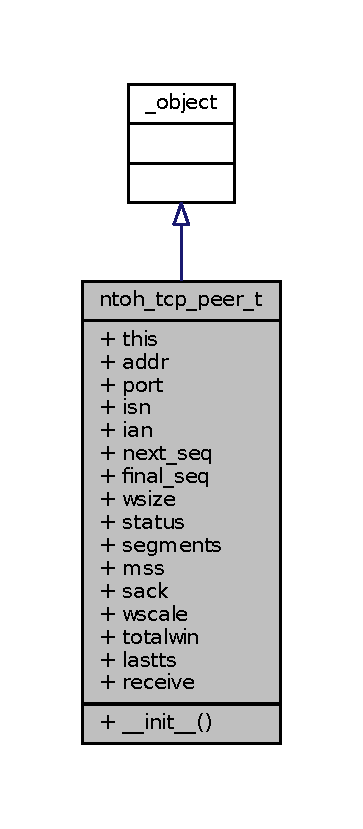
\includegraphics[width=174pt]{classlibntoh_1_1ntoh__tcp__peer__t__inherit__graph}
\end{center}
\end{figure}


Collaboration diagram for ntoh\-\_\-tcp\-\_\-peer\-\_\-t\-:
\nopagebreak
\begin{figure}[H]
\begin{center}
\leavevmode
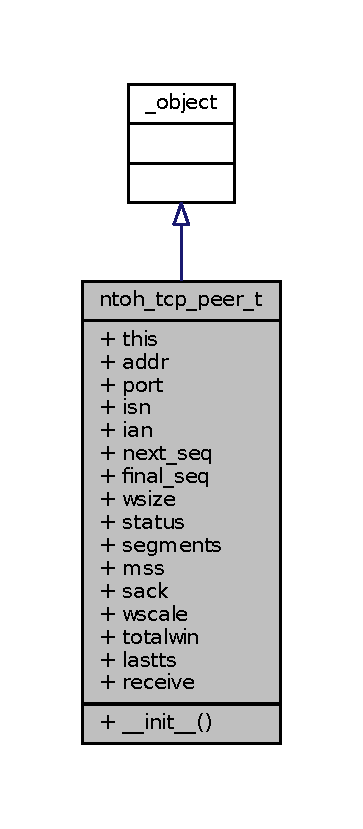
\includegraphics[width=174pt]{classlibntoh_1_1ntoh__tcp__peer__t__coll__graph}
\end{center}
\end{figure}
\subsection*{Public Member Functions}
\begin{DoxyCompactItemize}
\item 
def \hyperlink{classlibntoh_1_1ntoh__tcp__peer__t_ac775ee34451fdfa742b318538164070e}{\-\_\-\-\_\-init\-\_\-\-\_\-}
\end{DoxyCompactItemize}
\subsection*{Data Fields}
\begin{DoxyCompactItemize}
\item 
\hyperlink{classlibntoh_1_1ntoh__tcp__peer__t_a05c09a5e9d53fa7adf0a7936038c2fa3}{this}
\end{DoxyCompactItemize}
\subsection*{Static Public Attributes}
\begin{DoxyCompactItemize}
\item 
tuple \hyperlink{classlibntoh_1_1ntoh__tcp__peer__t_a2173c231c978de69ce30d0430739f1a1}{addr} = \hyperlink{namespacelibntoh_ae6f5626f776538e0cdb00e75ca1c96c9}{\-\_\-swig\-\_\-property}(\-\_\-libntoh.\-ntoh\-\_\-tcp\-\_\-peer\-\_\-t\-\_\-addr\-\_\-get, \-\_\-libntoh.\-ntoh\-\_\-tcp\-\_\-peer\-\_\-t\-\_\-addr\-\_\-set)
\item 
tuple \hyperlink{classlibntoh_1_1ntoh__tcp__peer__t_a1aadf525515ecfcf662c2aa51a503763}{port} = \hyperlink{namespacelibntoh_ae6f5626f776538e0cdb00e75ca1c96c9}{\-\_\-swig\-\_\-property}(\-\_\-libntoh.\-ntoh\-\_\-tcp\-\_\-peer\-\_\-t\-\_\-port\-\_\-get, \-\_\-libntoh.\-ntoh\-\_\-tcp\-\_\-peer\-\_\-t\-\_\-port\-\_\-set)
\item 
tuple \hyperlink{classlibntoh_1_1ntoh__tcp__peer__t_ab2f25f00739a355b0b11009767cebff1}{isn} = \hyperlink{namespacelibntoh_ae6f5626f776538e0cdb00e75ca1c96c9}{\-\_\-swig\-\_\-property}(\-\_\-libntoh.\-ntoh\-\_\-tcp\-\_\-peer\-\_\-t\-\_\-isn\-\_\-get, \-\_\-libntoh.\-ntoh\-\_\-tcp\-\_\-peer\-\_\-t\-\_\-isn\-\_\-set)
\item 
tuple \hyperlink{classlibntoh_1_1ntoh__tcp__peer__t_a6df1b754c46aba0b045b242e7db0fc73}{ian} = \hyperlink{namespacelibntoh_ae6f5626f776538e0cdb00e75ca1c96c9}{\-\_\-swig\-\_\-property}(\-\_\-libntoh.\-ntoh\-\_\-tcp\-\_\-peer\-\_\-t\-\_\-ian\-\_\-get, \-\_\-libntoh.\-ntoh\-\_\-tcp\-\_\-peer\-\_\-t\-\_\-ian\-\_\-set)
\item 
tuple \hyperlink{classlibntoh_1_1ntoh__tcp__peer__t_a48a6c283c2a56902dcf6b858f9e2ec46}{next\-\_\-seq} = \hyperlink{namespacelibntoh_ae6f5626f776538e0cdb00e75ca1c96c9}{\-\_\-swig\-\_\-property}(\-\_\-libntoh.\-ntoh\-\_\-tcp\-\_\-peer\-\_\-t\-\_\-next\-\_\-seq\-\_\-get, \-\_\-libntoh.\-ntoh\-\_\-tcp\-\_\-peer\-\_\-t\-\_\-next\-\_\-seq\-\_\-set)
\item 
tuple \hyperlink{classlibntoh_1_1ntoh__tcp__peer__t_acfbf6a8704c9a239a68087d6340fc2ab}{final\-\_\-seq} = \hyperlink{namespacelibntoh_ae6f5626f776538e0cdb00e75ca1c96c9}{\-\_\-swig\-\_\-property}(\-\_\-libntoh.\-ntoh\-\_\-tcp\-\_\-peer\-\_\-t\-\_\-final\-\_\-seq\-\_\-get, \-\_\-libntoh.\-ntoh\-\_\-tcp\-\_\-peer\-\_\-t\-\_\-final\-\_\-seq\-\_\-set)
\item 
tuple \hyperlink{classlibntoh_1_1ntoh__tcp__peer__t_a67662bf2129e6e2477a14aa1b8373e65}{wsize} = \hyperlink{namespacelibntoh_ae6f5626f776538e0cdb00e75ca1c96c9}{\-\_\-swig\-\_\-property}(\-\_\-libntoh.\-ntoh\-\_\-tcp\-\_\-peer\-\_\-t\-\_\-wsize\-\_\-get, \-\_\-libntoh.\-ntoh\-\_\-tcp\-\_\-peer\-\_\-t\-\_\-wsize\-\_\-set)
\item 
tuple \hyperlink{classlibntoh_1_1ntoh__tcp__peer__t_ad7843c85abee4764c9e717a8db8cb3a5}{status} = \hyperlink{namespacelibntoh_ae6f5626f776538e0cdb00e75ca1c96c9}{\-\_\-swig\-\_\-property}(\-\_\-libntoh.\-ntoh\-\_\-tcp\-\_\-peer\-\_\-t\-\_\-status\-\_\-get, \-\_\-libntoh.\-ntoh\-\_\-tcp\-\_\-peer\-\_\-t\-\_\-status\-\_\-set)
\item 
tuple \hyperlink{classlibntoh_1_1ntoh__tcp__peer__t_a54b6380f989a7f1215352bd7588e082d}{segments} = \hyperlink{namespacelibntoh_ae6f5626f776538e0cdb00e75ca1c96c9}{\-\_\-swig\-\_\-property}(\-\_\-libntoh.\-ntoh\-\_\-tcp\-\_\-peer\-\_\-t\-\_\-segments\-\_\-get, \-\_\-libntoh.\-ntoh\-\_\-tcp\-\_\-peer\-\_\-t\-\_\-segments\-\_\-set)
\item 
tuple \hyperlink{classlibntoh_1_1ntoh__tcp__peer__t_aecdeb465bed15a6124eddc5069330a88}{mss} = \hyperlink{namespacelibntoh_ae6f5626f776538e0cdb00e75ca1c96c9}{\-\_\-swig\-\_\-property}(\-\_\-libntoh.\-ntoh\-\_\-tcp\-\_\-peer\-\_\-t\-\_\-mss\-\_\-get, \-\_\-libntoh.\-ntoh\-\_\-tcp\-\_\-peer\-\_\-t\-\_\-mss\-\_\-set)
\item 
tuple \hyperlink{classlibntoh_1_1ntoh__tcp__peer__t_ae1f4a14905497ecba8d6687be3b9bcdd}{sack} = \hyperlink{namespacelibntoh_ae6f5626f776538e0cdb00e75ca1c96c9}{\-\_\-swig\-\_\-property}(\-\_\-libntoh.\-ntoh\-\_\-tcp\-\_\-peer\-\_\-t\-\_\-sack\-\_\-get, \-\_\-libntoh.\-ntoh\-\_\-tcp\-\_\-peer\-\_\-t\-\_\-sack\-\_\-set)
\item 
tuple \hyperlink{classlibntoh_1_1ntoh__tcp__peer__t_a17fc4fd78c94de2e5155e43de064f36c}{wscale} = \hyperlink{namespacelibntoh_ae6f5626f776538e0cdb00e75ca1c96c9}{\-\_\-swig\-\_\-property}(\-\_\-libntoh.\-ntoh\-\_\-tcp\-\_\-peer\-\_\-t\-\_\-wscale\-\_\-get, \-\_\-libntoh.\-ntoh\-\_\-tcp\-\_\-peer\-\_\-t\-\_\-wscale\-\_\-set)
\item 
tuple \hyperlink{classlibntoh_1_1ntoh__tcp__peer__t_a2806f6eb15dc5af0fbc1f184de81c626}{totalwin} = \hyperlink{namespacelibntoh_ae6f5626f776538e0cdb00e75ca1c96c9}{\-\_\-swig\-\_\-property}(\-\_\-libntoh.\-ntoh\-\_\-tcp\-\_\-peer\-\_\-t\-\_\-totalwin\-\_\-get, \-\_\-libntoh.\-ntoh\-\_\-tcp\-\_\-peer\-\_\-t\-\_\-totalwin\-\_\-set)
\item 
tuple \hyperlink{classlibntoh_1_1ntoh__tcp__peer__t_a2858fd84349a5843a79dd5daf529c04d}{lastts} = \hyperlink{namespacelibntoh_ae6f5626f776538e0cdb00e75ca1c96c9}{\-\_\-swig\-\_\-property}(\-\_\-libntoh.\-ntoh\-\_\-tcp\-\_\-peer\-\_\-t\-\_\-lastts\-\_\-get, \-\_\-libntoh.\-ntoh\-\_\-tcp\-\_\-peer\-\_\-t\-\_\-lastts\-\_\-set)
\item 
tuple \hyperlink{classlibntoh_1_1ntoh__tcp__peer__t_abe7dc0678d2658dea89330f2a7d15b7c}{receive} = \hyperlink{namespacelibntoh_ae6f5626f776538e0cdb00e75ca1c96c9}{\-\_\-swig\-\_\-property}(\-\_\-libntoh.\-ntoh\-\_\-tcp\-\_\-peer\-\_\-t\-\_\-receive\-\_\-get, \-\_\-libntoh.\-ntoh\-\_\-tcp\-\_\-peer\-\_\-t\-\_\-receive\-\_\-set)
\end{DoxyCompactItemize}


\subsection{Constructor \& Destructor Documentation}
\hypertarget{classlibntoh_1_1ntoh__tcp__peer__t_ac775ee34451fdfa742b318538164070e}{\index{libntoh\-::ntoh\-\_\-tcp\-\_\-peer\-\_\-t@{libntoh\-::ntoh\-\_\-tcp\-\_\-peer\-\_\-t}!\-\_\-\-\_\-init\-\_\-\-\_\-@{\-\_\-\-\_\-init\-\_\-\-\_\-}}
\index{\-\_\-\-\_\-init\-\_\-\-\_\-@{\-\_\-\-\_\-init\-\_\-\-\_\-}!libntoh::ntoh_tcp_peer_t@{libntoh\-::ntoh\-\_\-tcp\-\_\-peer\-\_\-t}}
\subsubsection[{\-\_\-\-\_\-init\-\_\-\-\_\-}]{\setlength{\rightskip}{0pt plus 5cm}def \-\_\-\-\_\-init\-\_\-\-\_\- (
\begin{DoxyParamCaption}
\item[{}]{self}
\end{DoxyParamCaption}
)}}\label{classlibntoh_1_1ntoh__tcp__peer__t_ac775ee34451fdfa742b318538164070e}


\subsection{Field Documentation}
\hypertarget{classlibntoh_1_1ntoh__tcp__peer__t_a2173c231c978de69ce30d0430739f1a1}{\index{libntoh\-::ntoh\-\_\-tcp\-\_\-peer\-\_\-t@{libntoh\-::ntoh\-\_\-tcp\-\_\-peer\-\_\-t}!addr@{addr}}
\index{addr@{addr}!libntoh::ntoh_tcp_peer_t@{libntoh\-::ntoh\-\_\-tcp\-\_\-peer\-\_\-t}}
\subsubsection[{addr}]{\setlength{\rightskip}{0pt plus 5cm}tuple addr = {\bf \-\_\-swig\-\_\-property}(\-\_\-libntoh.\-ntoh\-\_\-tcp\-\_\-peer\-\_\-t\-\_\-addr\-\_\-get, \-\_\-libntoh.\-ntoh\-\_\-tcp\-\_\-peer\-\_\-t\-\_\-addr\-\_\-set)\hspace{0.3cm}{\ttfamily [static]}}}\label{classlibntoh_1_1ntoh__tcp__peer__t_a2173c231c978de69ce30d0430739f1a1}
\hypertarget{classlibntoh_1_1ntoh__tcp__peer__t_acfbf6a8704c9a239a68087d6340fc2ab}{\index{libntoh\-::ntoh\-\_\-tcp\-\_\-peer\-\_\-t@{libntoh\-::ntoh\-\_\-tcp\-\_\-peer\-\_\-t}!final\-\_\-seq@{final\-\_\-seq}}
\index{final\-\_\-seq@{final\-\_\-seq}!libntoh::ntoh_tcp_peer_t@{libntoh\-::ntoh\-\_\-tcp\-\_\-peer\-\_\-t}}
\subsubsection[{final\-\_\-seq}]{\setlength{\rightskip}{0pt plus 5cm}tuple final\-\_\-seq = {\bf \-\_\-swig\-\_\-property}(\-\_\-libntoh.\-ntoh\-\_\-tcp\-\_\-peer\-\_\-t\-\_\-final\-\_\-seq\-\_\-get, \-\_\-libntoh.\-ntoh\-\_\-tcp\-\_\-peer\-\_\-t\-\_\-final\-\_\-seq\-\_\-set)\hspace{0.3cm}{\ttfamily [static]}}}\label{classlibntoh_1_1ntoh__tcp__peer__t_acfbf6a8704c9a239a68087d6340fc2ab}
\hypertarget{classlibntoh_1_1ntoh__tcp__peer__t_a6df1b754c46aba0b045b242e7db0fc73}{\index{libntoh\-::ntoh\-\_\-tcp\-\_\-peer\-\_\-t@{libntoh\-::ntoh\-\_\-tcp\-\_\-peer\-\_\-t}!ian@{ian}}
\index{ian@{ian}!libntoh::ntoh_tcp_peer_t@{libntoh\-::ntoh\-\_\-tcp\-\_\-peer\-\_\-t}}
\subsubsection[{ian}]{\setlength{\rightskip}{0pt plus 5cm}tuple ian = {\bf \-\_\-swig\-\_\-property}(\-\_\-libntoh.\-ntoh\-\_\-tcp\-\_\-peer\-\_\-t\-\_\-ian\-\_\-get, \-\_\-libntoh.\-ntoh\-\_\-tcp\-\_\-peer\-\_\-t\-\_\-ian\-\_\-set)\hspace{0.3cm}{\ttfamily [static]}}}\label{classlibntoh_1_1ntoh__tcp__peer__t_a6df1b754c46aba0b045b242e7db0fc73}
\hypertarget{classlibntoh_1_1ntoh__tcp__peer__t_ab2f25f00739a355b0b11009767cebff1}{\index{libntoh\-::ntoh\-\_\-tcp\-\_\-peer\-\_\-t@{libntoh\-::ntoh\-\_\-tcp\-\_\-peer\-\_\-t}!isn@{isn}}
\index{isn@{isn}!libntoh::ntoh_tcp_peer_t@{libntoh\-::ntoh\-\_\-tcp\-\_\-peer\-\_\-t}}
\subsubsection[{isn}]{\setlength{\rightskip}{0pt plus 5cm}tuple isn = {\bf \-\_\-swig\-\_\-property}(\-\_\-libntoh.\-ntoh\-\_\-tcp\-\_\-peer\-\_\-t\-\_\-isn\-\_\-get, \-\_\-libntoh.\-ntoh\-\_\-tcp\-\_\-peer\-\_\-t\-\_\-isn\-\_\-set)\hspace{0.3cm}{\ttfamily [static]}}}\label{classlibntoh_1_1ntoh__tcp__peer__t_ab2f25f00739a355b0b11009767cebff1}
\hypertarget{classlibntoh_1_1ntoh__tcp__peer__t_a2858fd84349a5843a79dd5daf529c04d}{\index{libntoh\-::ntoh\-\_\-tcp\-\_\-peer\-\_\-t@{libntoh\-::ntoh\-\_\-tcp\-\_\-peer\-\_\-t}!lastts@{lastts}}
\index{lastts@{lastts}!libntoh::ntoh_tcp_peer_t@{libntoh\-::ntoh\-\_\-tcp\-\_\-peer\-\_\-t}}
\subsubsection[{lastts}]{\setlength{\rightskip}{0pt plus 5cm}tuple lastts = {\bf \-\_\-swig\-\_\-property}(\-\_\-libntoh.\-ntoh\-\_\-tcp\-\_\-peer\-\_\-t\-\_\-lastts\-\_\-get, \-\_\-libntoh.\-ntoh\-\_\-tcp\-\_\-peer\-\_\-t\-\_\-lastts\-\_\-set)\hspace{0.3cm}{\ttfamily [static]}}}\label{classlibntoh_1_1ntoh__tcp__peer__t_a2858fd84349a5843a79dd5daf529c04d}
\hypertarget{classlibntoh_1_1ntoh__tcp__peer__t_aecdeb465bed15a6124eddc5069330a88}{\index{libntoh\-::ntoh\-\_\-tcp\-\_\-peer\-\_\-t@{libntoh\-::ntoh\-\_\-tcp\-\_\-peer\-\_\-t}!mss@{mss}}
\index{mss@{mss}!libntoh::ntoh_tcp_peer_t@{libntoh\-::ntoh\-\_\-tcp\-\_\-peer\-\_\-t}}
\subsubsection[{mss}]{\setlength{\rightskip}{0pt plus 5cm}tuple mss = {\bf \-\_\-swig\-\_\-property}(\-\_\-libntoh.\-ntoh\-\_\-tcp\-\_\-peer\-\_\-t\-\_\-mss\-\_\-get, \-\_\-libntoh.\-ntoh\-\_\-tcp\-\_\-peer\-\_\-t\-\_\-mss\-\_\-set)\hspace{0.3cm}{\ttfamily [static]}}}\label{classlibntoh_1_1ntoh__tcp__peer__t_aecdeb465bed15a6124eddc5069330a88}
\hypertarget{classlibntoh_1_1ntoh__tcp__peer__t_a48a6c283c2a56902dcf6b858f9e2ec46}{\index{libntoh\-::ntoh\-\_\-tcp\-\_\-peer\-\_\-t@{libntoh\-::ntoh\-\_\-tcp\-\_\-peer\-\_\-t}!next\-\_\-seq@{next\-\_\-seq}}
\index{next\-\_\-seq@{next\-\_\-seq}!libntoh::ntoh_tcp_peer_t@{libntoh\-::ntoh\-\_\-tcp\-\_\-peer\-\_\-t}}
\subsubsection[{next\-\_\-seq}]{\setlength{\rightskip}{0pt plus 5cm}tuple next\-\_\-seq = {\bf \-\_\-swig\-\_\-property}(\-\_\-libntoh.\-ntoh\-\_\-tcp\-\_\-peer\-\_\-t\-\_\-next\-\_\-seq\-\_\-get, \-\_\-libntoh.\-ntoh\-\_\-tcp\-\_\-peer\-\_\-t\-\_\-next\-\_\-seq\-\_\-set)\hspace{0.3cm}{\ttfamily [static]}}}\label{classlibntoh_1_1ntoh__tcp__peer__t_a48a6c283c2a56902dcf6b858f9e2ec46}
\hypertarget{classlibntoh_1_1ntoh__tcp__peer__t_a1aadf525515ecfcf662c2aa51a503763}{\index{libntoh\-::ntoh\-\_\-tcp\-\_\-peer\-\_\-t@{libntoh\-::ntoh\-\_\-tcp\-\_\-peer\-\_\-t}!port@{port}}
\index{port@{port}!libntoh::ntoh_tcp_peer_t@{libntoh\-::ntoh\-\_\-tcp\-\_\-peer\-\_\-t}}
\subsubsection[{port}]{\setlength{\rightskip}{0pt plus 5cm}tuple port = {\bf \-\_\-swig\-\_\-property}(\-\_\-libntoh.\-ntoh\-\_\-tcp\-\_\-peer\-\_\-t\-\_\-port\-\_\-get, \-\_\-libntoh.\-ntoh\-\_\-tcp\-\_\-peer\-\_\-t\-\_\-port\-\_\-set)\hspace{0.3cm}{\ttfamily [static]}}}\label{classlibntoh_1_1ntoh__tcp__peer__t_a1aadf525515ecfcf662c2aa51a503763}
\hypertarget{classlibntoh_1_1ntoh__tcp__peer__t_abe7dc0678d2658dea89330f2a7d15b7c}{\index{libntoh\-::ntoh\-\_\-tcp\-\_\-peer\-\_\-t@{libntoh\-::ntoh\-\_\-tcp\-\_\-peer\-\_\-t}!receive@{receive}}
\index{receive@{receive}!libntoh::ntoh_tcp_peer_t@{libntoh\-::ntoh\-\_\-tcp\-\_\-peer\-\_\-t}}
\subsubsection[{receive}]{\setlength{\rightskip}{0pt plus 5cm}tuple receive = {\bf \-\_\-swig\-\_\-property}(\-\_\-libntoh.\-ntoh\-\_\-tcp\-\_\-peer\-\_\-t\-\_\-receive\-\_\-get, \-\_\-libntoh.\-ntoh\-\_\-tcp\-\_\-peer\-\_\-t\-\_\-receive\-\_\-set)\hspace{0.3cm}{\ttfamily [static]}}}\label{classlibntoh_1_1ntoh__tcp__peer__t_abe7dc0678d2658dea89330f2a7d15b7c}
\hypertarget{classlibntoh_1_1ntoh__tcp__peer__t_ae1f4a14905497ecba8d6687be3b9bcdd}{\index{libntoh\-::ntoh\-\_\-tcp\-\_\-peer\-\_\-t@{libntoh\-::ntoh\-\_\-tcp\-\_\-peer\-\_\-t}!sack@{sack}}
\index{sack@{sack}!libntoh::ntoh_tcp_peer_t@{libntoh\-::ntoh\-\_\-tcp\-\_\-peer\-\_\-t}}
\subsubsection[{sack}]{\setlength{\rightskip}{0pt plus 5cm}tuple sack = {\bf \-\_\-swig\-\_\-property}(\-\_\-libntoh.\-ntoh\-\_\-tcp\-\_\-peer\-\_\-t\-\_\-sack\-\_\-get, \-\_\-libntoh.\-ntoh\-\_\-tcp\-\_\-peer\-\_\-t\-\_\-sack\-\_\-set)\hspace{0.3cm}{\ttfamily [static]}}}\label{classlibntoh_1_1ntoh__tcp__peer__t_ae1f4a14905497ecba8d6687be3b9bcdd}
\hypertarget{classlibntoh_1_1ntoh__tcp__peer__t_a54b6380f989a7f1215352bd7588e082d}{\index{libntoh\-::ntoh\-\_\-tcp\-\_\-peer\-\_\-t@{libntoh\-::ntoh\-\_\-tcp\-\_\-peer\-\_\-t}!segments@{segments}}
\index{segments@{segments}!libntoh::ntoh_tcp_peer_t@{libntoh\-::ntoh\-\_\-tcp\-\_\-peer\-\_\-t}}
\subsubsection[{segments}]{\setlength{\rightskip}{0pt plus 5cm}tuple segments = {\bf \-\_\-swig\-\_\-property}(\-\_\-libntoh.\-ntoh\-\_\-tcp\-\_\-peer\-\_\-t\-\_\-segments\-\_\-get, \-\_\-libntoh.\-ntoh\-\_\-tcp\-\_\-peer\-\_\-t\-\_\-segments\-\_\-set)\hspace{0.3cm}{\ttfamily [static]}}}\label{classlibntoh_1_1ntoh__tcp__peer__t_a54b6380f989a7f1215352bd7588e082d}
\hypertarget{classlibntoh_1_1ntoh__tcp__peer__t_ad7843c85abee4764c9e717a8db8cb3a5}{\index{libntoh\-::ntoh\-\_\-tcp\-\_\-peer\-\_\-t@{libntoh\-::ntoh\-\_\-tcp\-\_\-peer\-\_\-t}!status@{status}}
\index{status@{status}!libntoh::ntoh_tcp_peer_t@{libntoh\-::ntoh\-\_\-tcp\-\_\-peer\-\_\-t}}
\subsubsection[{status}]{\setlength{\rightskip}{0pt plus 5cm}tuple status = {\bf \-\_\-swig\-\_\-property}(\-\_\-libntoh.\-ntoh\-\_\-tcp\-\_\-peer\-\_\-t\-\_\-status\-\_\-get, \-\_\-libntoh.\-ntoh\-\_\-tcp\-\_\-peer\-\_\-t\-\_\-status\-\_\-set)\hspace{0.3cm}{\ttfamily [static]}}}\label{classlibntoh_1_1ntoh__tcp__peer__t_ad7843c85abee4764c9e717a8db8cb3a5}
\hypertarget{classlibntoh_1_1ntoh__tcp__peer__t_a05c09a5e9d53fa7adf0a7936038c2fa3}{\index{libntoh\-::ntoh\-\_\-tcp\-\_\-peer\-\_\-t@{libntoh\-::ntoh\-\_\-tcp\-\_\-peer\-\_\-t}!this@{this}}
\index{this@{this}!libntoh::ntoh_tcp_peer_t@{libntoh\-::ntoh\-\_\-tcp\-\_\-peer\-\_\-t}}
\subsubsection[{this}]{\setlength{\rightskip}{0pt plus 5cm}this}}\label{classlibntoh_1_1ntoh__tcp__peer__t_a05c09a5e9d53fa7adf0a7936038c2fa3}
\hypertarget{classlibntoh_1_1ntoh__tcp__peer__t_a2806f6eb15dc5af0fbc1f184de81c626}{\index{libntoh\-::ntoh\-\_\-tcp\-\_\-peer\-\_\-t@{libntoh\-::ntoh\-\_\-tcp\-\_\-peer\-\_\-t}!totalwin@{totalwin}}
\index{totalwin@{totalwin}!libntoh::ntoh_tcp_peer_t@{libntoh\-::ntoh\-\_\-tcp\-\_\-peer\-\_\-t}}
\subsubsection[{totalwin}]{\setlength{\rightskip}{0pt plus 5cm}tuple totalwin = {\bf \-\_\-swig\-\_\-property}(\-\_\-libntoh.\-ntoh\-\_\-tcp\-\_\-peer\-\_\-t\-\_\-totalwin\-\_\-get, \-\_\-libntoh.\-ntoh\-\_\-tcp\-\_\-peer\-\_\-t\-\_\-totalwin\-\_\-set)\hspace{0.3cm}{\ttfamily [static]}}}\label{classlibntoh_1_1ntoh__tcp__peer__t_a2806f6eb15dc5af0fbc1f184de81c626}
\hypertarget{classlibntoh_1_1ntoh__tcp__peer__t_a17fc4fd78c94de2e5155e43de064f36c}{\index{libntoh\-::ntoh\-\_\-tcp\-\_\-peer\-\_\-t@{libntoh\-::ntoh\-\_\-tcp\-\_\-peer\-\_\-t}!wscale@{wscale}}
\index{wscale@{wscale}!libntoh::ntoh_tcp_peer_t@{libntoh\-::ntoh\-\_\-tcp\-\_\-peer\-\_\-t}}
\subsubsection[{wscale}]{\setlength{\rightskip}{0pt plus 5cm}tuple wscale = {\bf \-\_\-swig\-\_\-property}(\-\_\-libntoh.\-ntoh\-\_\-tcp\-\_\-peer\-\_\-t\-\_\-wscale\-\_\-get, \-\_\-libntoh.\-ntoh\-\_\-tcp\-\_\-peer\-\_\-t\-\_\-wscale\-\_\-set)\hspace{0.3cm}{\ttfamily [static]}}}\label{classlibntoh_1_1ntoh__tcp__peer__t_a17fc4fd78c94de2e5155e43de064f36c}
\hypertarget{classlibntoh_1_1ntoh__tcp__peer__t_a67662bf2129e6e2477a14aa1b8373e65}{\index{libntoh\-::ntoh\-\_\-tcp\-\_\-peer\-\_\-t@{libntoh\-::ntoh\-\_\-tcp\-\_\-peer\-\_\-t}!wsize@{wsize}}
\index{wsize@{wsize}!libntoh::ntoh_tcp_peer_t@{libntoh\-::ntoh\-\_\-tcp\-\_\-peer\-\_\-t}}
\subsubsection[{wsize}]{\setlength{\rightskip}{0pt plus 5cm}tuple wsize = {\bf \-\_\-swig\-\_\-property}(\-\_\-libntoh.\-ntoh\-\_\-tcp\-\_\-peer\-\_\-t\-\_\-wsize\-\_\-get, \-\_\-libntoh.\-ntoh\-\_\-tcp\-\_\-peer\-\_\-t\-\_\-wsize\-\_\-set)\hspace{0.3cm}{\ttfamily [static]}}}\label{classlibntoh_1_1ntoh__tcp__peer__t_a67662bf2129e6e2477a14aa1b8373e65}


The documentation for this class was generated from the following file\-:\begin{DoxyCompactItemize}
\item 
build/\hyperlink{libntoh_8py}{libntoh.\-py}\end{DoxyCompactItemize}

\hypertarget{classlibntoh_1_1ntoh__tcp__segment__t}{\section{ntoh\-\_\-tcp\-\_\-segment\-\_\-t Class Reference}
\label{classlibntoh_1_1ntoh__tcp__segment__t}\index{ntoh\-\_\-tcp\-\_\-segment\-\_\-t@{ntoh\-\_\-tcp\-\_\-segment\-\_\-t}}
}


Inheritance diagram for ntoh\-\_\-tcp\-\_\-segment\-\_\-t\-:
\nopagebreak
\begin{figure}[H]
\begin{center}
\leavevmode
\includegraphics[width=194pt]{classlibntoh_1_1ntoh__tcp__segment__t__inherit__graph}
\end{center}
\end{figure}


Collaboration diagram for ntoh\-\_\-tcp\-\_\-segment\-\_\-t\-:
\nopagebreak
\begin{figure}[H]
\begin{center}
\leavevmode
\includegraphics[width=194pt]{classlibntoh_1_1ntoh__tcp__segment__t__coll__graph}
\end{center}
\end{figure}
\subsection*{Public Member Functions}
\begin{DoxyCompactItemize}
\item 
def \hyperlink{classlibntoh_1_1ntoh__tcp__segment__t_ac775ee34451fdfa742b318538164070e}{\-\_\-\-\_\-init\-\_\-\-\_\-}
\end{DoxyCompactItemize}
\subsection*{Data Fields}
\begin{DoxyCompactItemize}
\item 
\hyperlink{classlibntoh_1_1ntoh__tcp__segment__t_a05c09a5e9d53fa7adf0a7936038c2fa3}{this}
\end{DoxyCompactItemize}
\subsection*{Static Public Attributes}
\begin{DoxyCompactItemize}
\item 
tuple \hyperlink{classlibntoh_1_1ntoh__tcp__segment__t_a84e6dac37062f5a539ece8248c8567cc}{next} = \hyperlink{namespacelibntoh_ae6f5626f776538e0cdb00e75ca1c96c9}{\-\_\-swig\-\_\-property}(\-\_\-libntoh.\-ntoh\-\_\-tcp\-\_\-segment\-\_\-t\-\_\-next\-\_\-get, \-\_\-libntoh.\-ntoh\-\_\-tcp\-\_\-segment\-\_\-t\-\_\-next\-\_\-set)
\item 
tuple \hyperlink{classlibntoh_1_1ntoh__tcp__segment__t_a716df55a3150c1225ef8612669f6b901}{seq} = \hyperlink{namespacelibntoh_ae6f5626f776538e0cdb00e75ca1c96c9}{\-\_\-swig\-\_\-property}(\-\_\-libntoh.\-ntoh\-\_\-tcp\-\_\-segment\-\_\-t\-\_\-seq\-\_\-get, \-\_\-libntoh.\-ntoh\-\_\-tcp\-\_\-segment\-\_\-t\-\_\-seq\-\_\-set)
\item 
tuple \hyperlink{classlibntoh_1_1ntoh__tcp__segment__t_a0ccc7a1fc96dc8394903666fc5eb23eb}{ack} = \hyperlink{namespacelibntoh_ae6f5626f776538e0cdb00e75ca1c96c9}{\-\_\-swig\-\_\-property}(\-\_\-libntoh.\-ntoh\-\_\-tcp\-\_\-segment\-\_\-t\-\_\-ack\-\_\-get, \-\_\-libntoh.\-ntoh\-\_\-tcp\-\_\-segment\-\_\-t\-\_\-ack\-\_\-set)
\item 
tuple \hyperlink{classlibntoh_1_1ntoh__tcp__segment__t_a9ceb38153d5c0f156fbeada6dc00ff4f}{flags} = \hyperlink{namespacelibntoh_ae6f5626f776538e0cdb00e75ca1c96c9}{\-\_\-swig\-\_\-property}(\-\_\-libntoh.\-ntoh\-\_\-tcp\-\_\-segment\-\_\-t\-\_\-flags\-\_\-get, \-\_\-libntoh.\-ntoh\-\_\-tcp\-\_\-segment\-\_\-t\-\_\-flags\-\_\-set)
\item 
tuple \hyperlink{classlibntoh_1_1ntoh__tcp__segment__t_a2d1aae70ae5f00aa8688e5a4004af497}{payload\-\_\-len} = \hyperlink{namespacelibntoh_ae6f5626f776538e0cdb00e75ca1c96c9}{\-\_\-swig\-\_\-property}(\-\_\-libntoh.\-ntoh\-\_\-tcp\-\_\-segment\-\_\-t\-\_\-payload\-\_\-len\-\_\-get, \-\_\-libntoh.\-ntoh\-\_\-tcp\-\_\-segment\-\_\-t\-\_\-payload\-\_\-len\-\_\-set)
\item 
tuple \hyperlink{classlibntoh_1_1ntoh__tcp__segment__t_a8b9d7517c215a6690dc57a59f2e58a46}{origin} = \hyperlink{namespacelibntoh_ae6f5626f776538e0cdb00e75ca1c96c9}{\-\_\-swig\-\_\-property}(\-\_\-libntoh.\-ntoh\-\_\-tcp\-\_\-segment\-\_\-t\-\_\-origin\-\_\-get, \-\_\-libntoh.\-ntoh\-\_\-tcp\-\_\-segment\-\_\-t\-\_\-origin\-\_\-set)
\item 
tuple \hyperlink{classlibntoh_1_1ntoh__tcp__segment__t_ae8cd99ed1999062cbd69ce770384d6e4}{tv} = \hyperlink{namespacelibntoh_ae6f5626f776538e0cdb00e75ca1c96c9}{\-\_\-swig\-\_\-property}(\-\_\-libntoh.\-ntoh\-\_\-tcp\-\_\-segment\-\_\-t\-\_\-tv\-\_\-get, \-\_\-libntoh.\-ntoh\-\_\-tcp\-\_\-segment\-\_\-t\-\_\-tv\-\_\-set)
\item 
tuple \hyperlink{classlibntoh_1_1ntoh__tcp__segment__t_a12e096cd679ca576247a83b9fd1d62e4}{user\-\_\-data} = \hyperlink{namespacelibntoh_ae6f5626f776538e0cdb00e75ca1c96c9}{\-\_\-swig\-\_\-property}(\-\_\-libntoh.\-ntoh\-\_\-tcp\-\_\-segment\-\_\-t\-\_\-user\-\_\-data\-\_\-get, \-\_\-libntoh.\-ntoh\-\_\-tcp\-\_\-segment\-\_\-t\-\_\-user\-\_\-data\-\_\-set)
\end{DoxyCompactItemize}


\subsection{Constructor \& Destructor Documentation}
\hypertarget{classlibntoh_1_1ntoh__tcp__segment__t_ac775ee34451fdfa742b318538164070e}{\index{libntoh\-::ntoh\-\_\-tcp\-\_\-segment\-\_\-t@{libntoh\-::ntoh\-\_\-tcp\-\_\-segment\-\_\-t}!\-\_\-\-\_\-init\-\_\-\-\_\-@{\-\_\-\-\_\-init\-\_\-\-\_\-}}
\index{\-\_\-\-\_\-init\-\_\-\-\_\-@{\-\_\-\-\_\-init\-\_\-\-\_\-}!libntoh::ntoh_tcp_segment_t@{libntoh\-::ntoh\-\_\-tcp\-\_\-segment\-\_\-t}}
\subsubsection[{\-\_\-\-\_\-init\-\_\-\-\_\-}]{\setlength{\rightskip}{0pt plus 5cm}def \-\_\-\-\_\-init\-\_\-\-\_\- (
\begin{DoxyParamCaption}
\item[{}]{self}
\end{DoxyParamCaption}
)}}\label{classlibntoh_1_1ntoh__tcp__segment__t_ac775ee34451fdfa742b318538164070e}


\subsection{Field Documentation}
\hypertarget{classlibntoh_1_1ntoh__tcp__segment__t_a0ccc7a1fc96dc8394903666fc5eb23eb}{\index{libntoh\-::ntoh\-\_\-tcp\-\_\-segment\-\_\-t@{libntoh\-::ntoh\-\_\-tcp\-\_\-segment\-\_\-t}!ack@{ack}}
\index{ack@{ack}!libntoh::ntoh_tcp_segment_t@{libntoh\-::ntoh\-\_\-tcp\-\_\-segment\-\_\-t}}
\subsubsection[{ack}]{\setlength{\rightskip}{0pt plus 5cm}tuple ack = {\bf \-\_\-swig\-\_\-property}(\-\_\-libntoh.\-ntoh\-\_\-tcp\-\_\-segment\-\_\-t\-\_\-ack\-\_\-get, \-\_\-libntoh.\-ntoh\-\_\-tcp\-\_\-segment\-\_\-t\-\_\-ack\-\_\-set)\hspace{0.3cm}{\ttfamily [static]}}}\label{classlibntoh_1_1ntoh__tcp__segment__t_a0ccc7a1fc96dc8394903666fc5eb23eb}
\hypertarget{classlibntoh_1_1ntoh__tcp__segment__t_a9ceb38153d5c0f156fbeada6dc00ff4f}{\index{libntoh\-::ntoh\-\_\-tcp\-\_\-segment\-\_\-t@{libntoh\-::ntoh\-\_\-tcp\-\_\-segment\-\_\-t}!flags@{flags}}
\index{flags@{flags}!libntoh::ntoh_tcp_segment_t@{libntoh\-::ntoh\-\_\-tcp\-\_\-segment\-\_\-t}}
\subsubsection[{flags}]{\setlength{\rightskip}{0pt plus 5cm}tuple flags = {\bf \-\_\-swig\-\_\-property}(\-\_\-libntoh.\-ntoh\-\_\-tcp\-\_\-segment\-\_\-t\-\_\-flags\-\_\-get, \-\_\-libntoh.\-ntoh\-\_\-tcp\-\_\-segment\-\_\-t\-\_\-flags\-\_\-set)\hspace{0.3cm}{\ttfamily [static]}}}\label{classlibntoh_1_1ntoh__tcp__segment__t_a9ceb38153d5c0f156fbeada6dc00ff4f}
\hypertarget{classlibntoh_1_1ntoh__tcp__segment__t_a84e6dac37062f5a539ece8248c8567cc}{\index{libntoh\-::ntoh\-\_\-tcp\-\_\-segment\-\_\-t@{libntoh\-::ntoh\-\_\-tcp\-\_\-segment\-\_\-t}!next@{next}}
\index{next@{next}!libntoh::ntoh_tcp_segment_t@{libntoh\-::ntoh\-\_\-tcp\-\_\-segment\-\_\-t}}
\subsubsection[{next}]{\setlength{\rightskip}{0pt plus 5cm}tuple next = {\bf \-\_\-swig\-\_\-property}(\-\_\-libntoh.\-ntoh\-\_\-tcp\-\_\-segment\-\_\-t\-\_\-next\-\_\-get, \-\_\-libntoh.\-ntoh\-\_\-tcp\-\_\-segment\-\_\-t\-\_\-next\-\_\-set)\hspace{0.3cm}{\ttfamily [static]}}}\label{classlibntoh_1_1ntoh__tcp__segment__t_a84e6dac37062f5a539ece8248c8567cc}
\hypertarget{classlibntoh_1_1ntoh__tcp__segment__t_a8b9d7517c215a6690dc57a59f2e58a46}{\index{libntoh\-::ntoh\-\_\-tcp\-\_\-segment\-\_\-t@{libntoh\-::ntoh\-\_\-tcp\-\_\-segment\-\_\-t}!origin@{origin}}
\index{origin@{origin}!libntoh::ntoh_tcp_segment_t@{libntoh\-::ntoh\-\_\-tcp\-\_\-segment\-\_\-t}}
\subsubsection[{origin}]{\setlength{\rightskip}{0pt plus 5cm}tuple origin = {\bf \-\_\-swig\-\_\-property}(\-\_\-libntoh.\-ntoh\-\_\-tcp\-\_\-segment\-\_\-t\-\_\-origin\-\_\-get, \-\_\-libntoh.\-ntoh\-\_\-tcp\-\_\-segment\-\_\-t\-\_\-origin\-\_\-set)\hspace{0.3cm}{\ttfamily [static]}}}\label{classlibntoh_1_1ntoh__tcp__segment__t_a8b9d7517c215a6690dc57a59f2e58a46}
\hypertarget{classlibntoh_1_1ntoh__tcp__segment__t_a2d1aae70ae5f00aa8688e5a4004af497}{\index{libntoh\-::ntoh\-\_\-tcp\-\_\-segment\-\_\-t@{libntoh\-::ntoh\-\_\-tcp\-\_\-segment\-\_\-t}!payload\-\_\-len@{payload\-\_\-len}}
\index{payload\-\_\-len@{payload\-\_\-len}!libntoh::ntoh_tcp_segment_t@{libntoh\-::ntoh\-\_\-tcp\-\_\-segment\-\_\-t}}
\subsubsection[{payload\-\_\-len}]{\setlength{\rightskip}{0pt plus 5cm}tuple payload\-\_\-len = {\bf \-\_\-swig\-\_\-property}(\-\_\-libntoh.\-ntoh\-\_\-tcp\-\_\-segment\-\_\-t\-\_\-payload\-\_\-len\-\_\-get, \-\_\-libntoh.\-ntoh\-\_\-tcp\-\_\-segment\-\_\-t\-\_\-payload\-\_\-len\-\_\-set)\hspace{0.3cm}{\ttfamily [static]}}}\label{classlibntoh_1_1ntoh__tcp__segment__t_a2d1aae70ae5f00aa8688e5a4004af497}
\hypertarget{classlibntoh_1_1ntoh__tcp__segment__t_a716df55a3150c1225ef8612669f6b901}{\index{libntoh\-::ntoh\-\_\-tcp\-\_\-segment\-\_\-t@{libntoh\-::ntoh\-\_\-tcp\-\_\-segment\-\_\-t}!seq@{seq}}
\index{seq@{seq}!libntoh::ntoh_tcp_segment_t@{libntoh\-::ntoh\-\_\-tcp\-\_\-segment\-\_\-t}}
\subsubsection[{seq}]{\setlength{\rightskip}{0pt plus 5cm}tuple seq = {\bf \-\_\-swig\-\_\-property}(\-\_\-libntoh.\-ntoh\-\_\-tcp\-\_\-segment\-\_\-t\-\_\-seq\-\_\-get, \-\_\-libntoh.\-ntoh\-\_\-tcp\-\_\-segment\-\_\-t\-\_\-seq\-\_\-set)\hspace{0.3cm}{\ttfamily [static]}}}\label{classlibntoh_1_1ntoh__tcp__segment__t_a716df55a3150c1225ef8612669f6b901}
\hypertarget{classlibntoh_1_1ntoh__tcp__segment__t_a05c09a5e9d53fa7adf0a7936038c2fa3}{\index{libntoh\-::ntoh\-\_\-tcp\-\_\-segment\-\_\-t@{libntoh\-::ntoh\-\_\-tcp\-\_\-segment\-\_\-t}!this@{this}}
\index{this@{this}!libntoh::ntoh_tcp_segment_t@{libntoh\-::ntoh\-\_\-tcp\-\_\-segment\-\_\-t}}
\subsubsection[{this}]{\setlength{\rightskip}{0pt plus 5cm}this}}\label{classlibntoh_1_1ntoh__tcp__segment__t_a05c09a5e9d53fa7adf0a7936038c2fa3}
\hypertarget{classlibntoh_1_1ntoh__tcp__segment__t_ae8cd99ed1999062cbd69ce770384d6e4}{\index{libntoh\-::ntoh\-\_\-tcp\-\_\-segment\-\_\-t@{libntoh\-::ntoh\-\_\-tcp\-\_\-segment\-\_\-t}!tv@{tv}}
\index{tv@{tv}!libntoh::ntoh_tcp_segment_t@{libntoh\-::ntoh\-\_\-tcp\-\_\-segment\-\_\-t}}
\subsubsection[{tv}]{\setlength{\rightskip}{0pt plus 5cm}tuple tv = {\bf \-\_\-swig\-\_\-property}(\-\_\-libntoh.\-ntoh\-\_\-tcp\-\_\-segment\-\_\-t\-\_\-tv\-\_\-get, \-\_\-libntoh.\-ntoh\-\_\-tcp\-\_\-segment\-\_\-t\-\_\-tv\-\_\-set)\hspace{0.3cm}{\ttfamily [static]}}}\label{classlibntoh_1_1ntoh__tcp__segment__t_ae8cd99ed1999062cbd69ce770384d6e4}
\hypertarget{classlibntoh_1_1ntoh__tcp__segment__t_a12e096cd679ca576247a83b9fd1d62e4}{\index{libntoh\-::ntoh\-\_\-tcp\-\_\-segment\-\_\-t@{libntoh\-::ntoh\-\_\-tcp\-\_\-segment\-\_\-t}!user\-\_\-data@{user\-\_\-data}}
\index{user\-\_\-data@{user\-\_\-data}!libntoh::ntoh_tcp_segment_t@{libntoh\-::ntoh\-\_\-tcp\-\_\-segment\-\_\-t}}
\subsubsection[{user\-\_\-data}]{\setlength{\rightskip}{0pt plus 5cm}tuple user\-\_\-data = {\bf \-\_\-swig\-\_\-property}(\-\_\-libntoh.\-ntoh\-\_\-tcp\-\_\-segment\-\_\-t\-\_\-user\-\_\-data\-\_\-get, \-\_\-libntoh.\-ntoh\-\_\-tcp\-\_\-segment\-\_\-t\-\_\-user\-\_\-data\-\_\-set)\hspace{0.3cm}{\ttfamily [static]}}}\label{classlibntoh_1_1ntoh__tcp__segment__t_a12e096cd679ca576247a83b9fd1d62e4}


The documentation for this class was generated from the following file\-:\begin{DoxyCompactItemize}
\item 
build/\hyperlink{libntoh_8py}{libntoh.\-py}\end{DoxyCompactItemize}

\hypertarget{classlibntoh_1_1ntoh__tcp__session__t}{\section{ntoh\-\_\-tcp\-\_\-session\-\_\-t Class Reference}
\label{classlibntoh_1_1ntoh__tcp__session__t}\index{ntoh\-\_\-tcp\-\_\-session\-\_\-t@{ntoh\-\_\-tcp\-\_\-session\-\_\-t}}
}


Inheritance diagram for ntoh\-\_\-tcp\-\_\-session\-\_\-t\-:
\nopagebreak
\begin{figure}[H]
\begin{center}
\leavevmode
\includegraphics[width=188pt]{classlibntoh_1_1ntoh__tcp__session__t__inherit__graph}
\end{center}
\end{figure}


Collaboration diagram for ntoh\-\_\-tcp\-\_\-session\-\_\-t\-:
\nopagebreak
\begin{figure}[H]
\begin{center}
\leavevmode
\includegraphics[width=188pt]{classlibntoh_1_1ntoh__tcp__session__t__coll__graph}
\end{center}
\end{figure}
\subsection*{Public Member Functions}
\begin{DoxyCompactItemize}
\item 
def \hyperlink{classlibntoh_1_1ntoh__tcp__session__t_ac775ee34451fdfa742b318538164070e}{\-\_\-\-\_\-init\-\_\-\-\_\-}
\end{DoxyCompactItemize}
\subsection*{Data Fields}
\begin{DoxyCompactItemize}
\item 
\hyperlink{classlibntoh_1_1ntoh__tcp__session__t_a05c09a5e9d53fa7adf0a7936038c2fa3}{this}
\end{DoxyCompactItemize}
\subsection*{Static Public Attributes}
\begin{DoxyCompactItemize}
\item 
tuple \hyperlink{classlibntoh_1_1ntoh__tcp__session__t_a84e6dac37062f5a539ece8248c8567cc}{next} = \hyperlink{namespacelibntoh_ae6f5626f776538e0cdb00e75ca1c96c9}{\-\_\-swig\-\_\-property}(\-\_\-libntoh.\-ntoh\-\_\-tcp\-\_\-session\-\_\-t\-\_\-next\-\_\-get, \-\_\-libntoh.\-ntoh\-\_\-tcp\-\_\-session\-\_\-t\-\_\-next\-\_\-set)
\item 
tuple \hyperlink{classlibntoh_1_1ntoh__tcp__session__t_ab08551f389ac2ec08b906a250a850739}{max\-\_\-streams} = \hyperlink{namespacelibntoh_ae6f5626f776538e0cdb00e75ca1c96c9}{\-\_\-swig\-\_\-property}(\-\_\-libntoh.\-ntoh\-\_\-tcp\-\_\-session\-\_\-t\-\_\-max\-\_\-streams\-\_\-get, \-\_\-libntoh.\-ntoh\-\_\-tcp\-\_\-session\-\_\-t\-\_\-max\-\_\-streams\-\_\-set)
\item 
tuple \hyperlink{classlibntoh_1_1ntoh__tcp__session__t_ad01cf9ea23f35bfa4d5bab3c0f182e42}{max\-\_\-timewait} = \hyperlink{namespacelibntoh_ae6f5626f776538e0cdb00e75ca1c96c9}{\-\_\-swig\-\_\-property}(\-\_\-libntoh.\-ntoh\-\_\-tcp\-\_\-session\-\_\-t\-\_\-max\-\_\-timewait\-\_\-get, \-\_\-libntoh.\-ntoh\-\_\-tcp\-\_\-session\-\_\-t\-\_\-max\-\_\-timewait\-\_\-set)
\item 
tuple \hyperlink{classlibntoh_1_1ntoh__tcp__session__t_a89d606a1c25ff8a032d2716489f69fcc}{streams} = \hyperlink{namespacelibntoh_ae6f5626f776538e0cdb00e75ca1c96c9}{\-\_\-swig\-\_\-property}(\-\_\-libntoh.\-ntoh\-\_\-tcp\-\_\-session\-\_\-t\-\_\-streams\-\_\-get, \-\_\-libntoh.\-ntoh\-\_\-tcp\-\_\-session\-\_\-t\-\_\-streams\-\_\-set)
\item 
tuple \hyperlink{classlibntoh_1_1ntoh__tcp__session__t_a5dfb36debadedad1db9bdc1ad97ab821}{timewait} = \hyperlink{namespacelibntoh_ae6f5626f776538e0cdb00e75ca1c96c9}{\-\_\-swig\-\_\-property}(\-\_\-libntoh.\-ntoh\-\_\-tcp\-\_\-session\-\_\-t\-\_\-timewait\-\_\-get, \-\_\-libntoh.\-ntoh\-\_\-tcp\-\_\-session\-\_\-t\-\_\-timewait\-\_\-set)
\item 
tuple \hyperlink{classlibntoh_1_1ntoh__tcp__session__t_afdb09afb7e6838badc0bf2a63b8df8c5}{rand} = \hyperlink{namespacelibntoh_ae6f5626f776538e0cdb00e75ca1c96c9}{\-\_\-swig\-\_\-property}(\-\_\-libntoh.\-ntoh\-\_\-tcp\-\_\-session\-\_\-t\-\_\-rand\-\_\-get, \-\_\-libntoh.\-ntoh\-\_\-tcp\-\_\-session\-\_\-t\-\_\-rand\-\_\-set)
\item 
tuple \hyperlink{classlibntoh_1_1ntoh__tcp__session__t_a871c7bf899334194698c2a3bced5e064}{lock} = \hyperlink{namespacelibntoh_ae6f5626f776538e0cdb00e75ca1c96c9}{\-\_\-swig\-\_\-property}(\-\_\-libntoh.\-ntoh\-\_\-tcp\-\_\-session\-\_\-t\-\_\-lock\-\_\-get, \-\_\-libntoh.\-ntoh\-\_\-tcp\-\_\-session\-\_\-t\-\_\-lock\-\_\-set)
\item 
tuple \hyperlink{classlibntoh_1_1ntoh__tcp__session__t_aa8af5c32a2a96a7fe7e14b7ebd2057ba}{t\-I\-D} = \hyperlink{namespacelibntoh_ae6f5626f776538e0cdb00e75ca1c96c9}{\-\_\-swig\-\_\-property}(\-\_\-libntoh.\-ntoh\-\_\-tcp\-\_\-session\-\_\-t\-\_\-t\-I\-D\-\_\-get, \-\_\-libntoh.\-ntoh\-\_\-tcp\-\_\-session\-\_\-t\-\_\-t\-I\-D\-\_\-set)
\end{DoxyCompactItemize}


\subsection{Constructor \& Destructor Documentation}
\hypertarget{classlibntoh_1_1ntoh__tcp__session__t_ac775ee34451fdfa742b318538164070e}{\index{libntoh\-::ntoh\-\_\-tcp\-\_\-session\-\_\-t@{libntoh\-::ntoh\-\_\-tcp\-\_\-session\-\_\-t}!\-\_\-\-\_\-init\-\_\-\-\_\-@{\-\_\-\-\_\-init\-\_\-\-\_\-}}
\index{\-\_\-\-\_\-init\-\_\-\-\_\-@{\-\_\-\-\_\-init\-\_\-\-\_\-}!libntoh::ntoh_tcp_session_t@{libntoh\-::ntoh\-\_\-tcp\-\_\-session\-\_\-t}}
\subsubsection[{\-\_\-\-\_\-init\-\_\-\-\_\-}]{\setlength{\rightskip}{0pt plus 5cm}def \-\_\-\-\_\-init\-\_\-\-\_\- (
\begin{DoxyParamCaption}
\item[{}]{self}
\end{DoxyParamCaption}
)}}\label{classlibntoh_1_1ntoh__tcp__session__t_ac775ee34451fdfa742b318538164070e}


\subsection{Field Documentation}
\hypertarget{classlibntoh_1_1ntoh__tcp__session__t_a871c7bf899334194698c2a3bced5e064}{\index{libntoh\-::ntoh\-\_\-tcp\-\_\-session\-\_\-t@{libntoh\-::ntoh\-\_\-tcp\-\_\-session\-\_\-t}!lock@{lock}}
\index{lock@{lock}!libntoh::ntoh_tcp_session_t@{libntoh\-::ntoh\-\_\-tcp\-\_\-session\-\_\-t}}
\subsubsection[{lock}]{\setlength{\rightskip}{0pt plus 5cm}tuple lock = {\bf \-\_\-swig\-\_\-property}(\-\_\-libntoh.\-ntoh\-\_\-tcp\-\_\-session\-\_\-t\-\_\-lock\-\_\-get, \-\_\-libntoh.\-ntoh\-\_\-tcp\-\_\-session\-\_\-t\-\_\-lock\-\_\-set)\hspace{0.3cm}{\ttfamily [static]}}}\label{classlibntoh_1_1ntoh__tcp__session__t_a871c7bf899334194698c2a3bced5e064}
\hypertarget{classlibntoh_1_1ntoh__tcp__session__t_ab08551f389ac2ec08b906a250a850739}{\index{libntoh\-::ntoh\-\_\-tcp\-\_\-session\-\_\-t@{libntoh\-::ntoh\-\_\-tcp\-\_\-session\-\_\-t}!max\-\_\-streams@{max\-\_\-streams}}
\index{max\-\_\-streams@{max\-\_\-streams}!libntoh::ntoh_tcp_session_t@{libntoh\-::ntoh\-\_\-tcp\-\_\-session\-\_\-t}}
\subsubsection[{max\-\_\-streams}]{\setlength{\rightskip}{0pt plus 5cm}tuple max\-\_\-streams = {\bf \-\_\-swig\-\_\-property}(\-\_\-libntoh.\-ntoh\-\_\-tcp\-\_\-session\-\_\-t\-\_\-max\-\_\-streams\-\_\-get, \-\_\-libntoh.\-ntoh\-\_\-tcp\-\_\-session\-\_\-t\-\_\-max\-\_\-streams\-\_\-set)\hspace{0.3cm}{\ttfamily [static]}}}\label{classlibntoh_1_1ntoh__tcp__session__t_ab08551f389ac2ec08b906a250a850739}
\hypertarget{classlibntoh_1_1ntoh__tcp__session__t_ad01cf9ea23f35bfa4d5bab3c0f182e42}{\index{libntoh\-::ntoh\-\_\-tcp\-\_\-session\-\_\-t@{libntoh\-::ntoh\-\_\-tcp\-\_\-session\-\_\-t}!max\-\_\-timewait@{max\-\_\-timewait}}
\index{max\-\_\-timewait@{max\-\_\-timewait}!libntoh::ntoh_tcp_session_t@{libntoh\-::ntoh\-\_\-tcp\-\_\-session\-\_\-t}}
\subsubsection[{max\-\_\-timewait}]{\setlength{\rightskip}{0pt plus 5cm}tuple max\-\_\-timewait = {\bf \-\_\-swig\-\_\-property}(\-\_\-libntoh.\-ntoh\-\_\-tcp\-\_\-session\-\_\-t\-\_\-max\-\_\-timewait\-\_\-get, \-\_\-libntoh.\-ntoh\-\_\-tcp\-\_\-session\-\_\-t\-\_\-max\-\_\-timewait\-\_\-set)\hspace{0.3cm}{\ttfamily [static]}}}\label{classlibntoh_1_1ntoh__tcp__session__t_ad01cf9ea23f35bfa4d5bab3c0f182e42}
\hypertarget{classlibntoh_1_1ntoh__tcp__session__t_a84e6dac37062f5a539ece8248c8567cc}{\index{libntoh\-::ntoh\-\_\-tcp\-\_\-session\-\_\-t@{libntoh\-::ntoh\-\_\-tcp\-\_\-session\-\_\-t}!next@{next}}
\index{next@{next}!libntoh::ntoh_tcp_session_t@{libntoh\-::ntoh\-\_\-tcp\-\_\-session\-\_\-t}}
\subsubsection[{next}]{\setlength{\rightskip}{0pt plus 5cm}tuple next = {\bf \-\_\-swig\-\_\-property}(\-\_\-libntoh.\-ntoh\-\_\-tcp\-\_\-session\-\_\-t\-\_\-next\-\_\-get, \-\_\-libntoh.\-ntoh\-\_\-tcp\-\_\-session\-\_\-t\-\_\-next\-\_\-set)\hspace{0.3cm}{\ttfamily [static]}}}\label{classlibntoh_1_1ntoh__tcp__session__t_a84e6dac37062f5a539ece8248c8567cc}
\hypertarget{classlibntoh_1_1ntoh__tcp__session__t_afdb09afb7e6838badc0bf2a63b8df8c5}{\index{libntoh\-::ntoh\-\_\-tcp\-\_\-session\-\_\-t@{libntoh\-::ntoh\-\_\-tcp\-\_\-session\-\_\-t}!rand@{rand}}
\index{rand@{rand}!libntoh::ntoh_tcp_session_t@{libntoh\-::ntoh\-\_\-tcp\-\_\-session\-\_\-t}}
\subsubsection[{rand}]{\setlength{\rightskip}{0pt plus 5cm}tuple rand = {\bf \-\_\-swig\-\_\-property}(\-\_\-libntoh.\-ntoh\-\_\-tcp\-\_\-session\-\_\-t\-\_\-rand\-\_\-get, \-\_\-libntoh.\-ntoh\-\_\-tcp\-\_\-session\-\_\-t\-\_\-rand\-\_\-set)\hspace{0.3cm}{\ttfamily [static]}}}\label{classlibntoh_1_1ntoh__tcp__session__t_afdb09afb7e6838badc0bf2a63b8df8c5}
\hypertarget{classlibntoh_1_1ntoh__tcp__session__t_a89d606a1c25ff8a032d2716489f69fcc}{\index{libntoh\-::ntoh\-\_\-tcp\-\_\-session\-\_\-t@{libntoh\-::ntoh\-\_\-tcp\-\_\-session\-\_\-t}!streams@{streams}}
\index{streams@{streams}!libntoh::ntoh_tcp_session_t@{libntoh\-::ntoh\-\_\-tcp\-\_\-session\-\_\-t}}
\subsubsection[{streams}]{\setlength{\rightskip}{0pt plus 5cm}tuple streams = {\bf \-\_\-swig\-\_\-property}(\-\_\-libntoh.\-ntoh\-\_\-tcp\-\_\-session\-\_\-t\-\_\-streams\-\_\-get, \-\_\-libntoh.\-ntoh\-\_\-tcp\-\_\-session\-\_\-t\-\_\-streams\-\_\-set)\hspace{0.3cm}{\ttfamily [static]}}}\label{classlibntoh_1_1ntoh__tcp__session__t_a89d606a1c25ff8a032d2716489f69fcc}
\hypertarget{classlibntoh_1_1ntoh__tcp__session__t_a05c09a5e9d53fa7adf0a7936038c2fa3}{\index{libntoh\-::ntoh\-\_\-tcp\-\_\-session\-\_\-t@{libntoh\-::ntoh\-\_\-tcp\-\_\-session\-\_\-t}!this@{this}}
\index{this@{this}!libntoh::ntoh_tcp_session_t@{libntoh\-::ntoh\-\_\-tcp\-\_\-session\-\_\-t}}
\subsubsection[{this}]{\setlength{\rightskip}{0pt plus 5cm}this}}\label{classlibntoh_1_1ntoh__tcp__session__t_a05c09a5e9d53fa7adf0a7936038c2fa3}
\hypertarget{classlibntoh_1_1ntoh__tcp__session__t_aa8af5c32a2a96a7fe7e14b7ebd2057ba}{\index{libntoh\-::ntoh\-\_\-tcp\-\_\-session\-\_\-t@{libntoh\-::ntoh\-\_\-tcp\-\_\-session\-\_\-t}!t\-I\-D@{t\-I\-D}}
\index{t\-I\-D@{t\-I\-D}!libntoh::ntoh_tcp_session_t@{libntoh\-::ntoh\-\_\-tcp\-\_\-session\-\_\-t}}
\subsubsection[{t\-I\-D}]{\setlength{\rightskip}{0pt plus 5cm}tuple t\-I\-D = {\bf \-\_\-swig\-\_\-property}(\-\_\-libntoh.\-ntoh\-\_\-tcp\-\_\-session\-\_\-t\-\_\-t\-I\-D\-\_\-get, \-\_\-libntoh.\-ntoh\-\_\-tcp\-\_\-session\-\_\-t\-\_\-t\-I\-D\-\_\-set)\hspace{0.3cm}{\ttfamily [static]}}}\label{classlibntoh_1_1ntoh__tcp__session__t_aa8af5c32a2a96a7fe7e14b7ebd2057ba}
\hypertarget{classlibntoh_1_1ntoh__tcp__session__t_a5dfb36debadedad1db9bdc1ad97ab821}{\index{libntoh\-::ntoh\-\_\-tcp\-\_\-session\-\_\-t@{libntoh\-::ntoh\-\_\-tcp\-\_\-session\-\_\-t}!timewait@{timewait}}
\index{timewait@{timewait}!libntoh::ntoh_tcp_session_t@{libntoh\-::ntoh\-\_\-tcp\-\_\-session\-\_\-t}}
\subsubsection[{timewait}]{\setlength{\rightskip}{0pt plus 5cm}tuple timewait = {\bf \-\_\-swig\-\_\-property}(\-\_\-libntoh.\-ntoh\-\_\-tcp\-\_\-session\-\_\-t\-\_\-timewait\-\_\-get, \-\_\-libntoh.\-ntoh\-\_\-tcp\-\_\-session\-\_\-t\-\_\-timewait\-\_\-set)\hspace{0.3cm}{\ttfamily [static]}}}\label{classlibntoh_1_1ntoh__tcp__session__t_a5dfb36debadedad1db9bdc1ad97ab821}


The documentation for this class was generated from the following file\-:\begin{DoxyCompactItemize}
\item 
build/\hyperlink{libntoh_8py}{libntoh.\-py}\end{DoxyCompactItemize}

\hypertarget{classlibntoh_1_1ntoh__tcp__stream__t}{\section{ntoh\-\_\-tcp\-\_\-stream\-\_\-t Class Reference}
\label{classlibntoh_1_1ntoh__tcp__stream__t}\index{ntoh\-\_\-tcp\-\_\-stream\-\_\-t@{ntoh\-\_\-tcp\-\_\-stream\-\_\-t}}
}


Inheritance diagram for ntoh\-\_\-tcp\-\_\-stream\-\_\-t\-:
\nopagebreak
\begin{figure}[H]
\begin{center}
\leavevmode
\includegraphics[width=224pt]{classlibntoh_1_1ntoh__tcp__stream__t__inherit__graph}
\end{center}
\end{figure}


Collaboration diagram for ntoh\-\_\-tcp\-\_\-stream\-\_\-t\-:
\nopagebreak
\begin{figure}[H]
\begin{center}
\leavevmode
\includegraphics[width=224pt]{classlibntoh_1_1ntoh__tcp__stream__t__coll__graph}
\end{center}
\end{figure}
\subsection*{Public Member Functions}
\begin{DoxyCompactItemize}
\item 
def \hyperlink{classlibntoh_1_1ntoh__tcp__stream__t_ac775ee34451fdfa742b318538164070e}{\-\_\-\-\_\-init\-\_\-\-\_\-}
\end{DoxyCompactItemize}
\subsection*{Data Fields}
\begin{DoxyCompactItemize}
\item 
\hyperlink{classlibntoh_1_1ntoh__tcp__stream__t_a05c09a5e9d53fa7adf0a7936038c2fa3}{this}
\end{DoxyCompactItemize}
\subsection*{Static Public Attributes}
\begin{DoxyCompactItemize}
\item 
\hyperlink{classlibntoh_1_1ntoh__tcp__stream__t_a945ee80121c935cc2e86d758ecc70579}{tuple} \hyperlink{classlibntoh_1_1ntoh__tcp__stream__t_a84e6dac37062f5a539ece8248c8567cc}{next} = \hyperlink{namespacelibntoh_ae6f5626f776538e0cdb00e75ca1c96c9}{\-\_\-swig\-\_\-property}(\-\_\-libntoh.\-ntoh\-\_\-tcp\-\_\-stream\-\_\-t\-\_\-next\-\_\-get, \-\_\-libntoh.\-ntoh\-\_\-tcp\-\_\-stream\-\_\-t\-\_\-next\-\_\-set)
\item 
tuple \hyperlink{classlibntoh_1_1ntoh__tcp__stream__t_a945ee80121c935cc2e86d758ecc70579}{tuple} = \hyperlink{namespacelibntoh_ae6f5626f776538e0cdb00e75ca1c96c9}{\-\_\-swig\-\_\-property}(\-\_\-libntoh.\-ntoh\-\_\-tcp\-\_\-stream\-\_\-t\-\_\-tuple\-\_\-get, \-\_\-libntoh.\-ntoh\-\_\-tcp\-\_\-stream\-\_\-t\-\_\-tuple\-\_\-set)
\item 
\hyperlink{classlibntoh_1_1ntoh__tcp__stream__t_a945ee80121c935cc2e86d758ecc70579}{tuple} \hyperlink{classlibntoh_1_1ntoh__tcp__stream__t_aabcf5d3b98f85310bb8b763c3b935666}{client} = \hyperlink{namespacelibntoh_ae6f5626f776538e0cdb00e75ca1c96c9}{\-\_\-swig\-\_\-property}(\-\_\-libntoh.\-ntoh\-\_\-tcp\-\_\-stream\-\_\-t\-\_\-client\-\_\-get, \-\_\-libntoh.\-ntoh\-\_\-tcp\-\_\-stream\-\_\-t\-\_\-client\-\_\-set)
\item 
\hyperlink{classlibntoh_1_1ntoh__tcp__stream__t_a945ee80121c935cc2e86d758ecc70579}{tuple} \hyperlink{classlibntoh_1_1ntoh__tcp__stream__t_a3b90a824912f44140b739f0ddb0bbd84}{server} = \hyperlink{namespacelibntoh_ae6f5626f776538e0cdb00e75ca1c96c9}{\-\_\-swig\-\_\-property}(\-\_\-libntoh.\-ntoh\-\_\-tcp\-\_\-stream\-\_\-t\-\_\-server\-\_\-get, \-\_\-libntoh.\-ntoh\-\_\-tcp\-\_\-stream\-\_\-t\-\_\-server\-\_\-set)
\item 
\hyperlink{classlibntoh_1_1ntoh__tcp__stream__t_a945ee80121c935cc2e86d758ecc70579}{tuple} \hyperlink{classlibntoh_1_1ntoh__tcp__stream__t_a29eb8dd921f77e19e24a20bcd820c2ed}{key} = \hyperlink{namespacelibntoh_ae6f5626f776538e0cdb00e75ca1c96c9}{\-\_\-swig\-\_\-property}(\-\_\-libntoh.\-ntoh\-\_\-tcp\-\_\-stream\-\_\-t\-\_\-key\-\_\-get, \-\_\-libntoh.\-ntoh\-\_\-tcp\-\_\-stream\-\_\-t\-\_\-key\-\_\-set)
\item 
\hyperlink{classlibntoh_1_1ntoh__tcp__stream__t_a945ee80121c935cc2e86d758ecc70579}{tuple} \hyperlink{classlibntoh_1_1ntoh__tcp__stream__t_ad7843c85abee4764c9e717a8db8cb3a5}{status} = \hyperlink{namespacelibntoh_ae6f5626f776538e0cdb00e75ca1c96c9}{\-\_\-swig\-\_\-property}(\-\_\-libntoh.\-ntoh\-\_\-tcp\-\_\-stream\-\_\-t\-\_\-status\-\_\-get, \-\_\-libntoh.\-ntoh\-\_\-tcp\-\_\-stream\-\_\-t\-\_\-status\-\_\-set)
\item 
\hyperlink{classlibntoh_1_1ntoh__tcp__stream__t_a945ee80121c935cc2e86d758ecc70579}{tuple} \hyperlink{classlibntoh_1_1ntoh__tcp__stream__t_a736d15e1443bece09d760478e5f42c09}{closedby} = \hyperlink{namespacelibntoh_ae6f5626f776538e0cdb00e75ca1c96c9}{\-\_\-swig\-\_\-property}(\-\_\-libntoh.\-ntoh\-\_\-tcp\-\_\-stream\-\_\-t\-\_\-closedby\-\_\-get, \-\_\-libntoh.\-ntoh\-\_\-tcp\-\_\-stream\-\_\-t\-\_\-closedby\-\_\-set)
\item 
\hyperlink{classlibntoh_1_1ntoh__tcp__stream__t_a945ee80121c935cc2e86d758ecc70579}{tuple} \hyperlink{classlibntoh_1_1ntoh__tcp__stream__t_a543077174a1281b9d00884a11a040629}{function} = \hyperlink{namespacelibntoh_ae6f5626f776538e0cdb00e75ca1c96c9}{\-\_\-swig\-\_\-property}(\-\_\-libntoh.\-ntoh\-\_\-tcp\-\_\-stream\-\_\-t\-\_\-function\-\_\-get, \-\_\-libntoh.\-ntoh\-\_\-tcp\-\_\-stream\-\_\-t\-\_\-function\-\_\-set)
\item 
\hyperlink{classlibntoh_1_1ntoh__tcp__stream__t_a945ee80121c935cc2e86d758ecc70579}{tuple} \hyperlink{classlibntoh_1_1ntoh__tcp__stream__t_a43a06ba72aed8671dd1579dbf6f78b1a}{last\-\_\-activ} = \hyperlink{namespacelibntoh_ae6f5626f776538e0cdb00e75ca1c96c9}{\-\_\-swig\-\_\-property}(\-\_\-libntoh.\-ntoh\-\_\-tcp\-\_\-stream\-\_\-t\-\_\-last\-\_\-activ\-\_\-get, \-\_\-libntoh.\-ntoh\-\_\-tcp\-\_\-stream\-\_\-t\-\_\-last\-\_\-activ\-\_\-set)
\item 
\hyperlink{classlibntoh_1_1ntoh__tcp__stream__t_a945ee80121c935cc2e86d758ecc70579}{tuple} \hyperlink{classlibntoh_1_1ntoh__tcp__stream__t_a01107768ed3836fe4c2f2072c1c789c6}{syn\-\_\-retries} = \hyperlink{namespacelibntoh_ae6f5626f776538e0cdb00e75ca1c96c9}{\-\_\-swig\-\_\-property}(\-\_\-libntoh.\-ntoh\-\_\-tcp\-\_\-stream\-\_\-t\-\_\-syn\-\_\-retries\-\_\-get, \-\_\-libntoh.\-ntoh\-\_\-tcp\-\_\-stream\-\_\-t\-\_\-syn\-\_\-retries\-\_\-set)
\item 
\hyperlink{classlibntoh_1_1ntoh__tcp__stream__t_a945ee80121c935cc2e86d758ecc70579}{tuple} \hyperlink{classlibntoh_1_1ntoh__tcp__stream__t_a1a6b192c6b711327b1c200ab48945023}{synack\-\_\-retries} = \hyperlink{namespacelibntoh_ae6f5626f776538e0cdb00e75ca1c96c9}{\-\_\-swig\-\_\-property}(\-\_\-libntoh.\-ntoh\-\_\-tcp\-\_\-stream\-\_\-t\-\_\-synack\-\_\-retries\-\_\-get, \-\_\-libntoh.\-ntoh\-\_\-tcp\-\_\-stream\-\_\-t\-\_\-synack\-\_\-retries\-\_\-set)
\item 
\hyperlink{classlibntoh_1_1ntoh__tcp__stream__t_a945ee80121c935cc2e86d758ecc70579}{tuple} \hyperlink{classlibntoh_1_1ntoh__tcp__stream__t_a6900744e840ca75a67e020c38d143891}{udata} = \hyperlink{namespacelibntoh_ae6f5626f776538e0cdb00e75ca1c96c9}{\-\_\-swig\-\_\-property}(\-\_\-libntoh.\-ntoh\-\_\-tcp\-\_\-stream\-\_\-t\-\_\-udata\-\_\-get, \-\_\-libntoh.\-ntoh\-\_\-tcp\-\_\-stream\-\_\-t\-\_\-udata\-\_\-set)
\item 
\hyperlink{classlibntoh_1_1ntoh__tcp__stream__t_a945ee80121c935cc2e86d758ecc70579}{tuple} \hyperlink{classlibntoh_1_1ntoh__tcp__stream__t_a871c7bf899334194698c2a3bced5e064}{lock} = \hyperlink{namespacelibntoh_ae6f5626f776538e0cdb00e75ca1c96c9}{\-\_\-swig\-\_\-property}(\-\_\-libntoh.\-ntoh\-\_\-tcp\-\_\-stream\-\_\-t\-\_\-lock\-\_\-get, \-\_\-libntoh.\-ntoh\-\_\-tcp\-\_\-stream\-\_\-t\-\_\-lock\-\_\-set)
\item 
\hyperlink{classlibntoh_1_1ntoh__tcp__stream__t_a945ee80121c935cc2e86d758ecc70579}{tuple} \hyperlink{classlibntoh_1_1ntoh__tcp__stream__t_a0047b061bc7280f819c498e3d27487ce}{enable\-\_\-check\-\_\-timeout} = \hyperlink{namespacelibntoh_ae6f5626f776538e0cdb00e75ca1c96c9}{\-\_\-swig\-\_\-property}(\-\_\-libntoh.\-ntoh\-\_\-tcp\-\_\-stream\-\_\-t\-\_\-enable\-\_\-check\-\_\-timeout\-\_\-get, \-\_\-libntoh.\-ntoh\-\_\-tcp\-\_\-stream\-\_\-t\-\_\-enable\-\_\-check\-\_\-timeout\-\_\-set)
\item 
\hyperlink{classlibntoh_1_1ntoh__tcp__stream__t_a945ee80121c935cc2e86d758ecc70579}{tuple} \hyperlink{classlibntoh_1_1ntoh__tcp__stream__t_ad528a3c30634bf94345f9a1126bcad6a}{enable\-\_\-check\-\_\-nowindow} = \hyperlink{namespacelibntoh_ae6f5626f776538e0cdb00e75ca1c96c9}{\-\_\-swig\-\_\-property}(\-\_\-libntoh.\-ntoh\-\_\-tcp\-\_\-stream\-\_\-t\-\_\-enable\-\_\-check\-\_\-nowindow\-\_\-get, \-\_\-libntoh.\-ntoh\-\_\-tcp\-\_\-stream\-\_\-t\-\_\-enable\-\_\-check\-\_\-nowindow\-\_\-set)
\end{DoxyCompactItemize}


\subsection{Constructor \& Destructor Documentation}
\hypertarget{classlibntoh_1_1ntoh__tcp__stream__t_ac775ee34451fdfa742b318538164070e}{\index{libntoh\-::ntoh\-\_\-tcp\-\_\-stream\-\_\-t@{libntoh\-::ntoh\-\_\-tcp\-\_\-stream\-\_\-t}!\-\_\-\-\_\-init\-\_\-\-\_\-@{\-\_\-\-\_\-init\-\_\-\-\_\-}}
\index{\-\_\-\-\_\-init\-\_\-\-\_\-@{\-\_\-\-\_\-init\-\_\-\-\_\-}!libntoh::ntoh_tcp_stream_t@{libntoh\-::ntoh\-\_\-tcp\-\_\-stream\-\_\-t}}
\subsubsection[{\-\_\-\-\_\-init\-\_\-\-\_\-}]{\setlength{\rightskip}{0pt plus 5cm}def \-\_\-\-\_\-init\-\_\-\-\_\- (
\begin{DoxyParamCaption}
\item[{}]{self}
\end{DoxyParamCaption}
)}}\label{classlibntoh_1_1ntoh__tcp__stream__t_ac775ee34451fdfa742b318538164070e}


\subsection{Field Documentation}
\hypertarget{classlibntoh_1_1ntoh__tcp__stream__t_aabcf5d3b98f85310bb8b763c3b935666}{\index{libntoh\-::ntoh\-\_\-tcp\-\_\-stream\-\_\-t@{libntoh\-::ntoh\-\_\-tcp\-\_\-stream\-\_\-t}!client@{client}}
\index{client@{client}!libntoh::ntoh_tcp_stream_t@{libntoh\-::ntoh\-\_\-tcp\-\_\-stream\-\_\-t}}
\subsubsection[{client}]{\setlength{\rightskip}{0pt plus 5cm}{\bf tuple} client = {\bf \-\_\-swig\-\_\-property}(\-\_\-libntoh.\-ntoh\-\_\-tcp\-\_\-stream\-\_\-t\-\_\-client\-\_\-get, \-\_\-libntoh.\-ntoh\-\_\-tcp\-\_\-stream\-\_\-t\-\_\-client\-\_\-set)\hspace{0.3cm}{\ttfamily [static]}}}\label{classlibntoh_1_1ntoh__tcp__stream__t_aabcf5d3b98f85310bb8b763c3b935666}
\hypertarget{classlibntoh_1_1ntoh__tcp__stream__t_a736d15e1443bece09d760478e5f42c09}{\index{libntoh\-::ntoh\-\_\-tcp\-\_\-stream\-\_\-t@{libntoh\-::ntoh\-\_\-tcp\-\_\-stream\-\_\-t}!closedby@{closedby}}
\index{closedby@{closedby}!libntoh::ntoh_tcp_stream_t@{libntoh\-::ntoh\-\_\-tcp\-\_\-stream\-\_\-t}}
\subsubsection[{closedby}]{\setlength{\rightskip}{0pt plus 5cm}{\bf tuple} closedby = {\bf \-\_\-swig\-\_\-property}(\-\_\-libntoh.\-ntoh\-\_\-tcp\-\_\-stream\-\_\-t\-\_\-closedby\-\_\-get, \-\_\-libntoh.\-ntoh\-\_\-tcp\-\_\-stream\-\_\-t\-\_\-closedby\-\_\-set)\hspace{0.3cm}{\ttfamily [static]}}}\label{classlibntoh_1_1ntoh__tcp__stream__t_a736d15e1443bece09d760478e5f42c09}
\hypertarget{classlibntoh_1_1ntoh__tcp__stream__t_ad528a3c30634bf94345f9a1126bcad6a}{\index{libntoh\-::ntoh\-\_\-tcp\-\_\-stream\-\_\-t@{libntoh\-::ntoh\-\_\-tcp\-\_\-stream\-\_\-t}!enable\-\_\-check\-\_\-nowindow@{enable\-\_\-check\-\_\-nowindow}}
\index{enable\-\_\-check\-\_\-nowindow@{enable\-\_\-check\-\_\-nowindow}!libntoh::ntoh_tcp_stream_t@{libntoh\-::ntoh\-\_\-tcp\-\_\-stream\-\_\-t}}
\subsubsection[{enable\-\_\-check\-\_\-nowindow}]{\setlength{\rightskip}{0pt plus 5cm}{\bf tuple} enable\-\_\-check\-\_\-nowindow = {\bf \-\_\-swig\-\_\-property}(\-\_\-libntoh.\-ntoh\-\_\-tcp\-\_\-stream\-\_\-t\-\_\-enable\-\_\-check\-\_\-nowindow\-\_\-get, \-\_\-libntoh.\-ntoh\-\_\-tcp\-\_\-stream\-\_\-t\-\_\-enable\-\_\-check\-\_\-nowindow\-\_\-set)\hspace{0.3cm}{\ttfamily [static]}}}\label{classlibntoh_1_1ntoh__tcp__stream__t_ad528a3c30634bf94345f9a1126bcad6a}
\hypertarget{classlibntoh_1_1ntoh__tcp__stream__t_a0047b061bc7280f819c498e3d27487ce}{\index{libntoh\-::ntoh\-\_\-tcp\-\_\-stream\-\_\-t@{libntoh\-::ntoh\-\_\-tcp\-\_\-stream\-\_\-t}!enable\-\_\-check\-\_\-timeout@{enable\-\_\-check\-\_\-timeout}}
\index{enable\-\_\-check\-\_\-timeout@{enable\-\_\-check\-\_\-timeout}!libntoh::ntoh_tcp_stream_t@{libntoh\-::ntoh\-\_\-tcp\-\_\-stream\-\_\-t}}
\subsubsection[{enable\-\_\-check\-\_\-timeout}]{\setlength{\rightskip}{0pt plus 5cm}{\bf tuple} enable\-\_\-check\-\_\-timeout = {\bf \-\_\-swig\-\_\-property}(\-\_\-libntoh.\-ntoh\-\_\-tcp\-\_\-stream\-\_\-t\-\_\-enable\-\_\-check\-\_\-timeout\-\_\-get, \-\_\-libntoh.\-ntoh\-\_\-tcp\-\_\-stream\-\_\-t\-\_\-enable\-\_\-check\-\_\-timeout\-\_\-set)\hspace{0.3cm}{\ttfamily [static]}}}\label{classlibntoh_1_1ntoh__tcp__stream__t_a0047b061bc7280f819c498e3d27487ce}
\hypertarget{classlibntoh_1_1ntoh__tcp__stream__t_a543077174a1281b9d00884a11a040629}{\index{libntoh\-::ntoh\-\_\-tcp\-\_\-stream\-\_\-t@{libntoh\-::ntoh\-\_\-tcp\-\_\-stream\-\_\-t}!function@{function}}
\index{function@{function}!libntoh::ntoh_tcp_stream_t@{libntoh\-::ntoh\-\_\-tcp\-\_\-stream\-\_\-t}}
\subsubsection[{function}]{\setlength{\rightskip}{0pt plus 5cm}{\bf tuple} function = {\bf \-\_\-swig\-\_\-property}(\-\_\-libntoh.\-ntoh\-\_\-tcp\-\_\-stream\-\_\-t\-\_\-function\-\_\-get, \-\_\-libntoh.\-ntoh\-\_\-tcp\-\_\-stream\-\_\-t\-\_\-function\-\_\-set)\hspace{0.3cm}{\ttfamily [static]}}}\label{classlibntoh_1_1ntoh__tcp__stream__t_a543077174a1281b9d00884a11a040629}
\hypertarget{classlibntoh_1_1ntoh__tcp__stream__t_a29eb8dd921f77e19e24a20bcd820c2ed}{\index{libntoh\-::ntoh\-\_\-tcp\-\_\-stream\-\_\-t@{libntoh\-::ntoh\-\_\-tcp\-\_\-stream\-\_\-t}!key@{key}}
\index{key@{key}!libntoh::ntoh_tcp_stream_t@{libntoh\-::ntoh\-\_\-tcp\-\_\-stream\-\_\-t}}
\subsubsection[{key}]{\setlength{\rightskip}{0pt plus 5cm}{\bf tuple} key = {\bf \-\_\-swig\-\_\-property}(\-\_\-libntoh.\-ntoh\-\_\-tcp\-\_\-stream\-\_\-t\-\_\-key\-\_\-get, \-\_\-libntoh.\-ntoh\-\_\-tcp\-\_\-stream\-\_\-t\-\_\-key\-\_\-set)\hspace{0.3cm}{\ttfamily [static]}}}\label{classlibntoh_1_1ntoh__tcp__stream__t_a29eb8dd921f77e19e24a20bcd820c2ed}
\hypertarget{classlibntoh_1_1ntoh__tcp__stream__t_a43a06ba72aed8671dd1579dbf6f78b1a}{\index{libntoh\-::ntoh\-\_\-tcp\-\_\-stream\-\_\-t@{libntoh\-::ntoh\-\_\-tcp\-\_\-stream\-\_\-t}!last\-\_\-activ@{last\-\_\-activ}}
\index{last\-\_\-activ@{last\-\_\-activ}!libntoh::ntoh_tcp_stream_t@{libntoh\-::ntoh\-\_\-tcp\-\_\-stream\-\_\-t}}
\subsubsection[{last\-\_\-activ}]{\setlength{\rightskip}{0pt plus 5cm}{\bf tuple} last\-\_\-activ = {\bf \-\_\-swig\-\_\-property}(\-\_\-libntoh.\-ntoh\-\_\-tcp\-\_\-stream\-\_\-t\-\_\-last\-\_\-activ\-\_\-get, \-\_\-libntoh.\-ntoh\-\_\-tcp\-\_\-stream\-\_\-t\-\_\-last\-\_\-activ\-\_\-set)\hspace{0.3cm}{\ttfamily [static]}}}\label{classlibntoh_1_1ntoh__tcp__stream__t_a43a06ba72aed8671dd1579dbf6f78b1a}
\hypertarget{classlibntoh_1_1ntoh__tcp__stream__t_a871c7bf899334194698c2a3bced5e064}{\index{libntoh\-::ntoh\-\_\-tcp\-\_\-stream\-\_\-t@{libntoh\-::ntoh\-\_\-tcp\-\_\-stream\-\_\-t}!lock@{lock}}
\index{lock@{lock}!libntoh::ntoh_tcp_stream_t@{libntoh\-::ntoh\-\_\-tcp\-\_\-stream\-\_\-t}}
\subsubsection[{lock}]{\setlength{\rightskip}{0pt plus 5cm}{\bf tuple} lock = {\bf \-\_\-swig\-\_\-property}(\-\_\-libntoh.\-ntoh\-\_\-tcp\-\_\-stream\-\_\-t\-\_\-lock\-\_\-get, \-\_\-libntoh.\-ntoh\-\_\-tcp\-\_\-stream\-\_\-t\-\_\-lock\-\_\-set)\hspace{0.3cm}{\ttfamily [static]}}}\label{classlibntoh_1_1ntoh__tcp__stream__t_a871c7bf899334194698c2a3bced5e064}
\hypertarget{classlibntoh_1_1ntoh__tcp__stream__t_a84e6dac37062f5a539ece8248c8567cc}{\index{libntoh\-::ntoh\-\_\-tcp\-\_\-stream\-\_\-t@{libntoh\-::ntoh\-\_\-tcp\-\_\-stream\-\_\-t}!next@{next}}
\index{next@{next}!libntoh::ntoh_tcp_stream_t@{libntoh\-::ntoh\-\_\-tcp\-\_\-stream\-\_\-t}}
\subsubsection[{next}]{\setlength{\rightskip}{0pt plus 5cm}{\bf tuple} next = {\bf \-\_\-swig\-\_\-property}(\-\_\-libntoh.\-ntoh\-\_\-tcp\-\_\-stream\-\_\-t\-\_\-next\-\_\-get, \-\_\-libntoh.\-ntoh\-\_\-tcp\-\_\-stream\-\_\-t\-\_\-next\-\_\-set)\hspace{0.3cm}{\ttfamily [static]}}}\label{classlibntoh_1_1ntoh__tcp__stream__t_a84e6dac37062f5a539ece8248c8567cc}
\hypertarget{classlibntoh_1_1ntoh__tcp__stream__t_a3b90a824912f44140b739f0ddb0bbd84}{\index{libntoh\-::ntoh\-\_\-tcp\-\_\-stream\-\_\-t@{libntoh\-::ntoh\-\_\-tcp\-\_\-stream\-\_\-t}!server@{server}}
\index{server@{server}!libntoh::ntoh_tcp_stream_t@{libntoh\-::ntoh\-\_\-tcp\-\_\-stream\-\_\-t}}
\subsubsection[{server}]{\setlength{\rightskip}{0pt plus 5cm}{\bf tuple} server = {\bf \-\_\-swig\-\_\-property}(\-\_\-libntoh.\-ntoh\-\_\-tcp\-\_\-stream\-\_\-t\-\_\-server\-\_\-get, \-\_\-libntoh.\-ntoh\-\_\-tcp\-\_\-stream\-\_\-t\-\_\-server\-\_\-set)\hspace{0.3cm}{\ttfamily [static]}}}\label{classlibntoh_1_1ntoh__tcp__stream__t_a3b90a824912f44140b739f0ddb0bbd84}
\hypertarget{classlibntoh_1_1ntoh__tcp__stream__t_ad7843c85abee4764c9e717a8db8cb3a5}{\index{libntoh\-::ntoh\-\_\-tcp\-\_\-stream\-\_\-t@{libntoh\-::ntoh\-\_\-tcp\-\_\-stream\-\_\-t}!status@{status}}
\index{status@{status}!libntoh::ntoh_tcp_stream_t@{libntoh\-::ntoh\-\_\-tcp\-\_\-stream\-\_\-t}}
\subsubsection[{status}]{\setlength{\rightskip}{0pt plus 5cm}{\bf tuple} status = {\bf \-\_\-swig\-\_\-property}(\-\_\-libntoh.\-ntoh\-\_\-tcp\-\_\-stream\-\_\-t\-\_\-status\-\_\-get, \-\_\-libntoh.\-ntoh\-\_\-tcp\-\_\-stream\-\_\-t\-\_\-status\-\_\-set)\hspace{0.3cm}{\ttfamily [static]}}}\label{classlibntoh_1_1ntoh__tcp__stream__t_ad7843c85abee4764c9e717a8db8cb3a5}
\hypertarget{classlibntoh_1_1ntoh__tcp__stream__t_a01107768ed3836fe4c2f2072c1c789c6}{\index{libntoh\-::ntoh\-\_\-tcp\-\_\-stream\-\_\-t@{libntoh\-::ntoh\-\_\-tcp\-\_\-stream\-\_\-t}!syn\-\_\-retries@{syn\-\_\-retries}}
\index{syn\-\_\-retries@{syn\-\_\-retries}!libntoh::ntoh_tcp_stream_t@{libntoh\-::ntoh\-\_\-tcp\-\_\-stream\-\_\-t}}
\subsubsection[{syn\-\_\-retries}]{\setlength{\rightskip}{0pt plus 5cm}{\bf tuple} syn\-\_\-retries = {\bf \-\_\-swig\-\_\-property}(\-\_\-libntoh.\-ntoh\-\_\-tcp\-\_\-stream\-\_\-t\-\_\-syn\-\_\-retries\-\_\-get, \-\_\-libntoh.\-ntoh\-\_\-tcp\-\_\-stream\-\_\-t\-\_\-syn\-\_\-retries\-\_\-set)\hspace{0.3cm}{\ttfamily [static]}}}\label{classlibntoh_1_1ntoh__tcp__stream__t_a01107768ed3836fe4c2f2072c1c789c6}
\hypertarget{classlibntoh_1_1ntoh__tcp__stream__t_a1a6b192c6b711327b1c200ab48945023}{\index{libntoh\-::ntoh\-\_\-tcp\-\_\-stream\-\_\-t@{libntoh\-::ntoh\-\_\-tcp\-\_\-stream\-\_\-t}!synack\-\_\-retries@{synack\-\_\-retries}}
\index{synack\-\_\-retries@{synack\-\_\-retries}!libntoh::ntoh_tcp_stream_t@{libntoh\-::ntoh\-\_\-tcp\-\_\-stream\-\_\-t}}
\subsubsection[{synack\-\_\-retries}]{\setlength{\rightskip}{0pt plus 5cm}{\bf tuple} synack\-\_\-retries = {\bf \-\_\-swig\-\_\-property}(\-\_\-libntoh.\-ntoh\-\_\-tcp\-\_\-stream\-\_\-t\-\_\-synack\-\_\-retries\-\_\-get, \-\_\-libntoh.\-ntoh\-\_\-tcp\-\_\-stream\-\_\-t\-\_\-synack\-\_\-retries\-\_\-set)\hspace{0.3cm}{\ttfamily [static]}}}\label{classlibntoh_1_1ntoh__tcp__stream__t_a1a6b192c6b711327b1c200ab48945023}
\hypertarget{classlibntoh_1_1ntoh__tcp__stream__t_a05c09a5e9d53fa7adf0a7936038c2fa3}{\index{libntoh\-::ntoh\-\_\-tcp\-\_\-stream\-\_\-t@{libntoh\-::ntoh\-\_\-tcp\-\_\-stream\-\_\-t}!this@{this}}
\index{this@{this}!libntoh::ntoh_tcp_stream_t@{libntoh\-::ntoh\-\_\-tcp\-\_\-stream\-\_\-t}}
\subsubsection[{this}]{\setlength{\rightskip}{0pt plus 5cm}this}}\label{classlibntoh_1_1ntoh__tcp__stream__t_a05c09a5e9d53fa7adf0a7936038c2fa3}
\hypertarget{classlibntoh_1_1ntoh__tcp__stream__t_a945ee80121c935cc2e86d758ecc70579}{\index{libntoh\-::ntoh\-\_\-tcp\-\_\-stream\-\_\-t@{libntoh\-::ntoh\-\_\-tcp\-\_\-stream\-\_\-t}!tuple@{tuple}}
\index{tuple@{tuple}!libntoh::ntoh_tcp_stream_t@{libntoh\-::ntoh\-\_\-tcp\-\_\-stream\-\_\-t}}
\subsubsection[{tuple}]{\setlength{\rightskip}{0pt plus 5cm}tuple tuple = {\bf \-\_\-swig\-\_\-property}(\-\_\-libntoh.\-ntoh\-\_\-tcp\-\_\-stream\-\_\-t\-\_\-tuple\-\_\-get, \-\_\-libntoh.\-ntoh\-\_\-tcp\-\_\-stream\-\_\-t\-\_\-tuple\-\_\-set)\hspace{0.3cm}{\ttfamily [static]}}}\label{classlibntoh_1_1ntoh__tcp__stream__t_a945ee80121c935cc2e86d758ecc70579}
\hypertarget{classlibntoh_1_1ntoh__tcp__stream__t_a6900744e840ca75a67e020c38d143891}{\index{libntoh\-::ntoh\-\_\-tcp\-\_\-stream\-\_\-t@{libntoh\-::ntoh\-\_\-tcp\-\_\-stream\-\_\-t}!udata@{udata}}
\index{udata@{udata}!libntoh::ntoh_tcp_stream_t@{libntoh\-::ntoh\-\_\-tcp\-\_\-stream\-\_\-t}}
\subsubsection[{udata}]{\setlength{\rightskip}{0pt plus 5cm}{\bf tuple} udata = {\bf \-\_\-swig\-\_\-property}(\-\_\-libntoh.\-ntoh\-\_\-tcp\-\_\-stream\-\_\-t\-\_\-udata\-\_\-get, \-\_\-libntoh.\-ntoh\-\_\-tcp\-\_\-stream\-\_\-t\-\_\-udata\-\_\-set)\hspace{0.3cm}{\ttfamily [static]}}}\label{classlibntoh_1_1ntoh__tcp__stream__t_a6900744e840ca75a67e020c38d143891}


The documentation for this class was generated from the following file\-:\begin{DoxyCompactItemize}
\item 
build/\hyperlink{libntoh_8py}{libntoh.\-py}\end{DoxyCompactItemize}

\hypertarget{structntoh__tcp__tuple5__t}{\section{ntoh\-\_\-tcp\-\_\-tuple5\-\_\-t Struct Reference}
\label{structntoh__tcp__tuple5__t}\index{ntoh\-\_\-tcp\-\_\-tuple5\-\_\-t@{ntoh\-\_\-tcp\-\_\-tuple5\-\_\-t}}
}


data to generate the connection key  




{\ttfamily \#include $<$tcpreassembly.\-h$>$}



Collaboration diagram for ntoh\-\_\-tcp\-\_\-tuple5\-\_\-t\-:
\nopagebreak
\begin{figure}[H]
\begin{center}
\leavevmode
\includegraphics[width=182pt]{structntoh__tcp__tuple5__t__coll__graph}
\end{center}
\end{figure}
\subsection*{Data Fields}
\begin{DoxyCompactItemize}
\item 
unsigned int \hyperlink{structntoh__tcp__tuple5__t_a32ee136f9a3309d9f5aec70ddaebc420}{source}
\begin{DoxyCompactList}\small\item\em source address \end{DoxyCompactList}\item 
unsigned int \hyperlink{structntoh__tcp__tuple5__t_aa2b73075fb6a7866116ece24e01ea950}{destination}
\begin{DoxyCompactList}\small\item\em destination address \end{DoxyCompactList}\item 
unsigned short \hyperlink{structntoh__tcp__tuple5__t_a7122c66c4668cd4ee36485bd9009ca6d}{sport}
\begin{DoxyCompactList}\small\item\em source port \end{DoxyCompactList}\item 
unsigned short \hyperlink{structntoh__tcp__tuple5__t_a1fdc28da1e85b5968e0ce83dcb106287}{dport}
\begin{DoxyCompactList}\small\item\em destination port \end{DoxyCompactList}\item 
unsigned short \hyperlink{structntoh__tcp__tuple5__t_ac61644f2747d106fe73d2aba4384a2ba}{protocol}
\begin{DoxyCompactList}\small\item\em protocol \end{DoxyCompactList}\end{DoxyCompactItemize}


\subsection{Detailed Description}
data to generate the connection key 

\subsection{Field Documentation}
\hypertarget{structntoh__tcp__tuple5__t_aa2b73075fb6a7866116ece24e01ea950}{\index{ntoh\-\_\-tcp\-\_\-tuple5\-\_\-t@{ntoh\-\_\-tcp\-\_\-tuple5\-\_\-t}!destination@{destination}}
\index{destination@{destination}!ntoh_tcp_tuple5_t@{ntoh\-\_\-tcp\-\_\-tuple5\-\_\-t}}
\subsubsection[{destination}]{\setlength{\rightskip}{0pt plus 5cm}unsigned int destination}}\label{structntoh__tcp__tuple5__t_aa2b73075fb6a7866116ece24e01ea950}


destination address 

\hypertarget{structntoh__tcp__tuple5__t_a1fdc28da1e85b5968e0ce83dcb106287}{\index{ntoh\-\_\-tcp\-\_\-tuple5\-\_\-t@{ntoh\-\_\-tcp\-\_\-tuple5\-\_\-t}!dport@{dport}}
\index{dport@{dport}!ntoh_tcp_tuple5_t@{ntoh\-\_\-tcp\-\_\-tuple5\-\_\-t}}
\subsubsection[{dport}]{\setlength{\rightskip}{0pt plus 5cm}unsigned short dport}}\label{structntoh__tcp__tuple5__t_a1fdc28da1e85b5968e0ce83dcb106287}


destination port 

\hypertarget{structntoh__tcp__tuple5__t_ac61644f2747d106fe73d2aba4384a2ba}{\index{ntoh\-\_\-tcp\-\_\-tuple5\-\_\-t@{ntoh\-\_\-tcp\-\_\-tuple5\-\_\-t}!protocol@{protocol}}
\index{protocol@{protocol}!ntoh_tcp_tuple5_t@{ntoh\-\_\-tcp\-\_\-tuple5\-\_\-t}}
\subsubsection[{protocol}]{\setlength{\rightskip}{0pt plus 5cm}unsigned short protocol}}\label{structntoh__tcp__tuple5__t_ac61644f2747d106fe73d2aba4384a2ba}


protocol 

\hypertarget{structntoh__tcp__tuple5__t_a32ee136f9a3309d9f5aec70ddaebc420}{\index{ntoh\-\_\-tcp\-\_\-tuple5\-\_\-t@{ntoh\-\_\-tcp\-\_\-tuple5\-\_\-t}!source@{source}}
\index{source@{source}!ntoh_tcp_tuple5_t@{ntoh\-\_\-tcp\-\_\-tuple5\-\_\-t}}
\subsubsection[{source}]{\setlength{\rightskip}{0pt plus 5cm}unsigned int source}}\label{structntoh__tcp__tuple5__t_a32ee136f9a3309d9f5aec70ddaebc420}


source address 

\hypertarget{structntoh__tcp__tuple5__t_a7122c66c4668cd4ee36485bd9009ca6d}{\index{ntoh\-\_\-tcp\-\_\-tuple5\-\_\-t@{ntoh\-\_\-tcp\-\_\-tuple5\-\_\-t}!sport@{sport}}
\index{sport@{sport}!ntoh_tcp_tuple5_t@{ntoh\-\_\-tcp\-\_\-tuple5\-\_\-t}}
\subsubsection[{sport}]{\setlength{\rightskip}{0pt plus 5cm}unsigned short sport}}\label{structntoh__tcp__tuple5__t_a7122c66c4668cd4ee36485bd9009ca6d}


source port 



The documentation for this struct was generated from the following file\-:\begin{DoxyCompactItemize}
\item 
inc/\hyperlink{tcpreassembly_8h}{tcpreassembly.\-h}\end{DoxyCompactItemize}

\hypertarget{classlibntoh_1_1ntoh__tcp__tuple5__t}{\section{ntoh\-\_\-tcp\-\_\-tuple5\-\_\-t Class Reference}
\label{classlibntoh_1_1ntoh__tcp__tuple5__t}\index{ntoh\-\_\-tcp\-\_\-tuple5\-\_\-t@{ntoh\-\_\-tcp\-\_\-tuple5\-\_\-t}}
}


Inheritance diagram for ntoh\-\_\-tcp\-\_\-tuple5\-\_\-t\-:
\nopagebreak
\begin{figure}[H]
\begin{center}
\leavevmode
\includegraphics[width=182pt]{classlibntoh_1_1ntoh__tcp__tuple5__t__inherit__graph}
\end{center}
\end{figure}


Collaboration diagram for ntoh\-\_\-tcp\-\_\-tuple5\-\_\-t\-:
\nopagebreak
\begin{figure}[H]
\begin{center}
\leavevmode
\includegraphics[width=182pt]{classlibntoh_1_1ntoh__tcp__tuple5__t__coll__graph}
\end{center}
\end{figure}
\subsection*{Public Member Functions}
\begin{DoxyCompactItemize}
\item 
def \hyperlink{classlibntoh_1_1ntoh__tcp__tuple5__t_ac775ee34451fdfa742b318538164070e}{\-\_\-\-\_\-init\-\_\-\-\_\-}
\end{DoxyCompactItemize}
\subsection*{Data Fields}
\begin{DoxyCompactItemize}
\item 
\hyperlink{classlibntoh_1_1ntoh__tcp__tuple5__t_a05c09a5e9d53fa7adf0a7936038c2fa3}{this}
\end{DoxyCompactItemize}
\subsection*{Static Public Attributes}
\begin{DoxyCompactItemize}
\item 
tuple \hyperlink{classlibntoh_1_1ntoh__tcp__tuple5__t_aa873026052cc3e5ba03877243fcb7ecd}{source} = \hyperlink{namespacelibntoh_ae6f5626f776538e0cdb00e75ca1c96c9}{\-\_\-swig\-\_\-property}(\-\_\-libntoh.\-ntoh\-\_\-tcp\-\_\-tuple5\-\_\-t\-\_\-source\-\_\-get, \-\_\-libntoh.\-ntoh\-\_\-tcp\-\_\-tuple5\-\_\-t\-\_\-source\-\_\-set)
\item 
tuple \hyperlink{classlibntoh_1_1ntoh__tcp__tuple5__t_adaac82457baf1096d1c38cadf8123ce7}{destination} = \hyperlink{namespacelibntoh_ae6f5626f776538e0cdb00e75ca1c96c9}{\-\_\-swig\-\_\-property}(\-\_\-libntoh.\-ntoh\-\_\-tcp\-\_\-tuple5\-\_\-t\-\_\-destination\-\_\-get, \-\_\-libntoh.\-ntoh\-\_\-tcp\-\_\-tuple5\-\_\-t\-\_\-destination\-\_\-set)
\item 
tuple \hyperlink{classlibntoh_1_1ntoh__tcp__tuple5__t_a2833ef95f75538c4db32557cebba6eeb}{sport} = \hyperlink{namespacelibntoh_ae6f5626f776538e0cdb00e75ca1c96c9}{\-\_\-swig\-\_\-property}(\-\_\-libntoh.\-ntoh\-\_\-tcp\-\_\-tuple5\-\_\-t\-\_\-sport\-\_\-get, \-\_\-libntoh.\-ntoh\-\_\-tcp\-\_\-tuple5\-\_\-t\-\_\-sport\-\_\-set)
\item 
tuple \hyperlink{classlibntoh_1_1ntoh__tcp__tuple5__t_a5f69c896ed006fde20f09b7858fce13e}{dport} = \hyperlink{namespacelibntoh_ae6f5626f776538e0cdb00e75ca1c96c9}{\-\_\-swig\-\_\-property}(\-\_\-libntoh.\-ntoh\-\_\-tcp\-\_\-tuple5\-\_\-t\-\_\-dport\-\_\-get, \-\_\-libntoh.\-ntoh\-\_\-tcp\-\_\-tuple5\-\_\-t\-\_\-dport\-\_\-set)
\item 
tuple \hyperlink{classlibntoh_1_1ntoh__tcp__tuple5__t_ae535ff0dd346855882bd298a9e22bbc1}{protocol} = \hyperlink{namespacelibntoh_ae6f5626f776538e0cdb00e75ca1c96c9}{\-\_\-swig\-\_\-property}(\-\_\-libntoh.\-ntoh\-\_\-tcp\-\_\-tuple5\-\_\-t\-\_\-protocol\-\_\-get, \-\_\-libntoh.\-ntoh\-\_\-tcp\-\_\-tuple5\-\_\-t\-\_\-protocol\-\_\-set)
\end{DoxyCompactItemize}


\subsection{Constructor \& Destructor Documentation}
\hypertarget{classlibntoh_1_1ntoh__tcp__tuple5__t_ac775ee34451fdfa742b318538164070e}{\index{libntoh\-::ntoh\-\_\-tcp\-\_\-tuple5\-\_\-t@{libntoh\-::ntoh\-\_\-tcp\-\_\-tuple5\-\_\-t}!\-\_\-\-\_\-init\-\_\-\-\_\-@{\-\_\-\-\_\-init\-\_\-\-\_\-}}
\index{\-\_\-\-\_\-init\-\_\-\-\_\-@{\-\_\-\-\_\-init\-\_\-\-\_\-}!libntoh::ntoh_tcp_tuple5_t@{libntoh\-::ntoh\-\_\-tcp\-\_\-tuple5\-\_\-t}}
\subsubsection[{\-\_\-\-\_\-init\-\_\-\-\_\-}]{\setlength{\rightskip}{0pt plus 5cm}def \-\_\-\-\_\-init\-\_\-\-\_\- (
\begin{DoxyParamCaption}
\item[{}]{self}
\end{DoxyParamCaption}
)}}\label{classlibntoh_1_1ntoh__tcp__tuple5__t_ac775ee34451fdfa742b318538164070e}


\subsection{Field Documentation}
\hypertarget{classlibntoh_1_1ntoh__tcp__tuple5__t_adaac82457baf1096d1c38cadf8123ce7}{\index{libntoh\-::ntoh\-\_\-tcp\-\_\-tuple5\-\_\-t@{libntoh\-::ntoh\-\_\-tcp\-\_\-tuple5\-\_\-t}!destination@{destination}}
\index{destination@{destination}!libntoh::ntoh_tcp_tuple5_t@{libntoh\-::ntoh\-\_\-tcp\-\_\-tuple5\-\_\-t}}
\subsubsection[{destination}]{\setlength{\rightskip}{0pt plus 5cm}tuple destination = {\bf \-\_\-swig\-\_\-property}(\-\_\-libntoh.\-ntoh\-\_\-tcp\-\_\-tuple5\-\_\-t\-\_\-destination\-\_\-get, \-\_\-libntoh.\-ntoh\-\_\-tcp\-\_\-tuple5\-\_\-t\-\_\-destination\-\_\-set)\hspace{0.3cm}{\ttfamily [static]}}}\label{classlibntoh_1_1ntoh__tcp__tuple5__t_adaac82457baf1096d1c38cadf8123ce7}
\hypertarget{classlibntoh_1_1ntoh__tcp__tuple5__t_a5f69c896ed006fde20f09b7858fce13e}{\index{libntoh\-::ntoh\-\_\-tcp\-\_\-tuple5\-\_\-t@{libntoh\-::ntoh\-\_\-tcp\-\_\-tuple5\-\_\-t}!dport@{dport}}
\index{dport@{dport}!libntoh::ntoh_tcp_tuple5_t@{libntoh\-::ntoh\-\_\-tcp\-\_\-tuple5\-\_\-t}}
\subsubsection[{dport}]{\setlength{\rightskip}{0pt plus 5cm}tuple dport = {\bf \-\_\-swig\-\_\-property}(\-\_\-libntoh.\-ntoh\-\_\-tcp\-\_\-tuple5\-\_\-t\-\_\-dport\-\_\-get, \-\_\-libntoh.\-ntoh\-\_\-tcp\-\_\-tuple5\-\_\-t\-\_\-dport\-\_\-set)\hspace{0.3cm}{\ttfamily [static]}}}\label{classlibntoh_1_1ntoh__tcp__tuple5__t_a5f69c896ed006fde20f09b7858fce13e}
\hypertarget{classlibntoh_1_1ntoh__tcp__tuple5__t_ae535ff0dd346855882bd298a9e22bbc1}{\index{libntoh\-::ntoh\-\_\-tcp\-\_\-tuple5\-\_\-t@{libntoh\-::ntoh\-\_\-tcp\-\_\-tuple5\-\_\-t}!protocol@{protocol}}
\index{protocol@{protocol}!libntoh::ntoh_tcp_tuple5_t@{libntoh\-::ntoh\-\_\-tcp\-\_\-tuple5\-\_\-t}}
\subsubsection[{protocol}]{\setlength{\rightskip}{0pt plus 5cm}tuple protocol = {\bf \-\_\-swig\-\_\-property}(\-\_\-libntoh.\-ntoh\-\_\-tcp\-\_\-tuple5\-\_\-t\-\_\-protocol\-\_\-get, \-\_\-libntoh.\-ntoh\-\_\-tcp\-\_\-tuple5\-\_\-t\-\_\-protocol\-\_\-set)\hspace{0.3cm}{\ttfamily [static]}}}\label{classlibntoh_1_1ntoh__tcp__tuple5__t_ae535ff0dd346855882bd298a9e22bbc1}
\hypertarget{classlibntoh_1_1ntoh__tcp__tuple5__t_aa873026052cc3e5ba03877243fcb7ecd}{\index{libntoh\-::ntoh\-\_\-tcp\-\_\-tuple5\-\_\-t@{libntoh\-::ntoh\-\_\-tcp\-\_\-tuple5\-\_\-t}!source@{source}}
\index{source@{source}!libntoh::ntoh_tcp_tuple5_t@{libntoh\-::ntoh\-\_\-tcp\-\_\-tuple5\-\_\-t}}
\subsubsection[{source}]{\setlength{\rightskip}{0pt plus 5cm}tuple source = {\bf \-\_\-swig\-\_\-property}(\-\_\-libntoh.\-ntoh\-\_\-tcp\-\_\-tuple5\-\_\-t\-\_\-source\-\_\-get, \-\_\-libntoh.\-ntoh\-\_\-tcp\-\_\-tuple5\-\_\-t\-\_\-source\-\_\-set)\hspace{0.3cm}{\ttfamily [static]}}}\label{classlibntoh_1_1ntoh__tcp__tuple5__t_aa873026052cc3e5ba03877243fcb7ecd}
\hypertarget{classlibntoh_1_1ntoh__tcp__tuple5__t_a2833ef95f75538c4db32557cebba6eeb}{\index{libntoh\-::ntoh\-\_\-tcp\-\_\-tuple5\-\_\-t@{libntoh\-::ntoh\-\_\-tcp\-\_\-tuple5\-\_\-t}!sport@{sport}}
\index{sport@{sport}!libntoh::ntoh_tcp_tuple5_t@{libntoh\-::ntoh\-\_\-tcp\-\_\-tuple5\-\_\-t}}
\subsubsection[{sport}]{\setlength{\rightskip}{0pt plus 5cm}tuple sport = {\bf \-\_\-swig\-\_\-property}(\-\_\-libntoh.\-ntoh\-\_\-tcp\-\_\-tuple5\-\_\-t\-\_\-sport\-\_\-get, \-\_\-libntoh.\-ntoh\-\_\-tcp\-\_\-tuple5\-\_\-t\-\_\-sport\-\_\-set)\hspace{0.3cm}{\ttfamily [static]}}}\label{classlibntoh_1_1ntoh__tcp__tuple5__t_a2833ef95f75538c4db32557cebba6eeb}
\hypertarget{classlibntoh_1_1ntoh__tcp__tuple5__t_a05c09a5e9d53fa7adf0a7936038c2fa3}{\index{libntoh\-::ntoh\-\_\-tcp\-\_\-tuple5\-\_\-t@{libntoh\-::ntoh\-\_\-tcp\-\_\-tuple5\-\_\-t}!this@{this}}
\index{this@{this}!libntoh::ntoh_tcp_tuple5_t@{libntoh\-::ntoh\-\_\-tcp\-\_\-tuple5\-\_\-t}}
\subsubsection[{this}]{\setlength{\rightskip}{0pt plus 5cm}this}}\label{classlibntoh_1_1ntoh__tcp__tuple5__t_a05c09a5e9d53fa7adf0a7936038c2fa3}


The documentation for this class was generated from the following file\-:\begin{DoxyCompactItemize}
\item 
build/\hyperlink{libntoh_8py}{libntoh.\-py}\end{DoxyCompactItemize}

\hypertarget{struct_py_heap_type_object}{\section{Py\-Heap\-Type\-Object Struct Reference}
\label{struct_py_heap_type_object}\index{Py\-Heap\-Type\-Object@{Py\-Heap\-Type\-Object}}
}


Collaboration diagram for Py\-Heap\-Type\-Object\-:
\nopagebreak
\begin{figure}[H]
\begin{center}
\leavevmode
\includegraphics[width=184pt]{struct_py_heap_type_object__coll__graph}
\end{center}
\end{figure}
\subsection*{Data Fields}
\begin{DoxyCompactItemize}
\item 
Py\-Type\-Object \hyperlink{struct_py_heap_type_object_ab95029e45ed9e584a319da3910e6d36a}{type}
\item 
Py\-Number\-Methods \hyperlink{struct_py_heap_type_object_ae0163a9a768a792c634d23bc9f665731}{as\-\_\-number}
\item 
Py\-Mapping\-Methods \hyperlink{struct_py_heap_type_object_a21b313b07bf28b7521a963b9d356042e}{as\-\_\-mapping}
\item 
Py\-Sequence\-Methods \hyperlink{struct_py_heap_type_object_adce47a2fa55f6780397cc0f84852dbb8}{as\-\_\-sequence}
\item 
Py\-Buffer\-Procs \hyperlink{struct_py_heap_type_object_abe4978c8aa7ef37a8da46660d4ab34e0}{as\-\_\-buffer}
\item 
Py\-Object $\ast$ \hyperlink{struct_py_heap_type_object_ab3978d96531ad97f1c3139b11f771f98}{name}
\item 
Py\-Object $\ast$ \hyperlink{struct_py_heap_type_object_a7127cc956fe3cde2a6dddc6f50345417}{slots}
\end{DoxyCompactItemize}


\subsection{Field Documentation}
\hypertarget{struct_py_heap_type_object_abe4978c8aa7ef37a8da46660d4ab34e0}{\index{Py\-Heap\-Type\-Object@{Py\-Heap\-Type\-Object}!as\-\_\-buffer@{as\-\_\-buffer}}
\index{as\-\_\-buffer@{as\-\_\-buffer}!PyHeapTypeObject@{Py\-Heap\-Type\-Object}}
\subsubsection[{as\-\_\-buffer}]{\setlength{\rightskip}{0pt plus 5cm}Py\-Buffer\-Procs as\-\_\-buffer}}\label{struct_py_heap_type_object_abe4978c8aa7ef37a8da46660d4ab34e0}
\hypertarget{struct_py_heap_type_object_a21b313b07bf28b7521a963b9d356042e}{\index{Py\-Heap\-Type\-Object@{Py\-Heap\-Type\-Object}!as\-\_\-mapping@{as\-\_\-mapping}}
\index{as\-\_\-mapping@{as\-\_\-mapping}!PyHeapTypeObject@{Py\-Heap\-Type\-Object}}
\subsubsection[{as\-\_\-mapping}]{\setlength{\rightskip}{0pt plus 5cm}Py\-Mapping\-Methods as\-\_\-mapping}}\label{struct_py_heap_type_object_a21b313b07bf28b7521a963b9d356042e}
\hypertarget{struct_py_heap_type_object_ae0163a9a768a792c634d23bc9f665731}{\index{Py\-Heap\-Type\-Object@{Py\-Heap\-Type\-Object}!as\-\_\-number@{as\-\_\-number}}
\index{as\-\_\-number@{as\-\_\-number}!PyHeapTypeObject@{Py\-Heap\-Type\-Object}}
\subsubsection[{as\-\_\-number}]{\setlength{\rightskip}{0pt plus 5cm}Py\-Number\-Methods as\-\_\-number}}\label{struct_py_heap_type_object_ae0163a9a768a792c634d23bc9f665731}
\hypertarget{struct_py_heap_type_object_adce47a2fa55f6780397cc0f84852dbb8}{\index{Py\-Heap\-Type\-Object@{Py\-Heap\-Type\-Object}!as\-\_\-sequence@{as\-\_\-sequence}}
\index{as\-\_\-sequence@{as\-\_\-sequence}!PyHeapTypeObject@{Py\-Heap\-Type\-Object}}
\subsubsection[{as\-\_\-sequence}]{\setlength{\rightskip}{0pt plus 5cm}Py\-Sequence\-Methods as\-\_\-sequence}}\label{struct_py_heap_type_object_adce47a2fa55f6780397cc0f84852dbb8}
\hypertarget{struct_py_heap_type_object_ab3978d96531ad97f1c3139b11f771f98}{\index{Py\-Heap\-Type\-Object@{Py\-Heap\-Type\-Object}!name@{name}}
\index{name@{name}!PyHeapTypeObject@{Py\-Heap\-Type\-Object}}
\subsubsection[{name}]{\setlength{\rightskip}{0pt plus 5cm}Py\-Object$\ast$ name}}\label{struct_py_heap_type_object_ab3978d96531ad97f1c3139b11f771f98}
\hypertarget{struct_py_heap_type_object_a7127cc956fe3cde2a6dddc6f50345417}{\index{Py\-Heap\-Type\-Object@{Py\-Heap\-Type\-Object}!slots@{slots}}
\index{slots@{slots}!PyHeapTypeObject@{Py\-Heap\-Type\-Object}}
\subsubsection[{slots}]{\setlength{\rightskip}{0pt plus 5cm}Py\-Object $\ast$ slots}}\label{struct_py_heap_type_object_a7127cc956fe3cde2a6dddc6f50345417}
\hypertarget{struct_py_heap_type_object_ab95029e45ed9e584a319da3910e6d36a}{\index{Py\-Heap\-Type\-Object@{Py\-Heap\-Type\-Object}!type@{type}}
\index{type@{type}!PyHeapTypeObject@{Py\-Heap\-Type\-Object}}
\subsubsection[{type}]{\setlength{\rightskip}{0pt plus 5cm}Py\-Type\-Object type}}\label{struct_py_heap_type_object_ab95029e45ed9e584a319da3910e6d36a}


The documentation for this struct was generated from the following file\-:\begin{DoxyCompactItemize}
\item 
build/\hyperlink{libntoh_p_y_t_h_o_n__wrap_8c}{libntoh\-P\-Y\-T\-H\-O\-N\-\_\-wrap.\-c}\end{DoxyCompactItemize}

\hypertarget{structswig__cast__info}{\section{swig\-\_\-cast\-\_\-info Struct Reference}
\label{structswig__cast__info}\index{swig\-\_\-cast\-\_\-info@{swig\-\_\-cast\-\_\-info}}
}


Collaboration diagram for swig\-\_\-cast\-\_\-info\-:
\nopagebreak
\begin{figure}[H]
\begin{center}
\leavevmode
\includegraphics[width=222pt]{structswig__cast__info__coll__graph}
\end{center}
\end{figure}
\subsection*{Data Fields}
\begin{DoxyCompactItemize}
\item 
\hyperlink{structswig__type__info}{swig\-\_\-type\-\_\-info} $\ast$ \hyperlink{structswig__cast__info_aa19bc251346ad9ae4ecb3b4e34545a5d}{type}
\item 
\hyperlink{libntoh_p_y_t_h_o_n__wrap_8c_a2c314f22b391bfcaff5a11f4b76f66ec}{swig\-\_\-converter\-\_\-func} \hyperlink{structswig__cast__info_ab0c02ae209c86c1a920b1a6cbec7ec52}{converter}
\item 
struct \hyperlink{structswig__cast__info}{swig\-\_\-cast\-\_\-info} $\ast$ \hyperlink{structswig__cast__info_af4349454713002040fd3799016337b36}{next}
\item 
struct \hyperlink{structswig__cast__info}{swig\-\_\-cast\-\_\-info} $\ast$ \hyperlink{structswig__cast__info_ad21cc20a49152bc851275a6747e89493}{prev}
\end{DoxyCompactItemize}


\subsection{Field Documentation}
\hypertarget{structswig__cast__info_ab0c02ae209c86c1a920b1a6cbec7ec52}{\index{swig\-\_\-cast\-\_\-info@{swig\-\_\-cast\-\_\-info}!converter@{converter}}
\index{converter@{converter}!swig_cast_info@{swig\-\_\-cast\-\_\-info}}
\subsubsection[{converter}]{\setlength{\rightskip}{0pt plus 5cm}{\bf swig\-\_\-converter\-\_\-func} converter}}\label{structswig__cast__info_ab0c02ae209c86c1a920b1a6cbec7ec52}
\hypertarget{structswig__cast__info_af4349454713002040fd3799016337b36}{\index{swig\-\_\-cast\-\_\-info@{swig\-\_\-cast\-\_\-info}!next@{next}}
\index{next@{next}!swig_cast_info@{swig\-\_\-cast\-\_\-info}}
\subsubsection[{next}]{\setlength{\rightskip}{0pt plus 5cm}struct {\bf swig\-\_\-cast\-\_\-info}$\ast$ next}}\label{structswig__cast__info_af4349454713002040fd3799016337b36}
\hypertarget{structswig__cast__info_ad21cc20a49152bc851275a6747e89493}{\index{swig\-\_\-cast\-\_\-info@{swig\-\_\-cast\-\_\-info}!prev@{prev}}
\index{prev@{prev}!swig_cast_info@{swig\-\_\-cast\-\_\-info}}
\subsubsection[{prev}]{\setlength{\rightskip}{0pt plus 5cm}struct {\bf swig\-\_\-cast\-\_\-info}$\ast$ prev}}\label{structswig__cast__info_ad21cc20a49152bc851275a6747e89493}
\hypertarget{structswig__cast__info_aa19bc251346ad9ae4ecb3b4e34545a5d}{\index{swig\-\_\-cast\-\_\-info@{swig\-\_\-cast\-\_\-info}!type@{type}}
\index{type@{type}!swig_cast_info@{swig\-\_\-cast\-\_\-info}}
\subsubsection[{type}]{\setlength{\rightskip}{0pt plus 5cm}{\bf swig\-\_\-type\-\_\-info}$\ast$ type}}\label{structswig__cast__info_aa19bc251346ad9ae4ecb3b4e34545a5d}


The documentation for this struct was generated from the following file\-:\begin{DoxyCompactItemize}
\item 
build/\hyperlink{libntoh_p_y_t_h_o_n__wrap_8c}{libntoh\-P\-Y\-T\-H\-O\-N\-\_\-wrap.\-c}\end{DoxyCompactItemize}

\hypertarget{structswig__const__info}{\section{swig\-\_\-const\-\_\-info Struct Reference}
\label{structswig__const__info}\index{swig\-\_\-const\-\_\-info@{swig\-\_\-const\-\_\-info}}
}


Collaboration diagram for swig\-\_\-const\-\_\-info\-:
\nopagebreak
\begin{figure}[H]
\begin{center}
\leavevmode
\includegraphics[width=330pt]{structswig__const__info__coll__graph}
\end{center}
\end{figure}
\subsection*{Data Fields}
\begin{DoxyCompactItemize}
\item 
int \hyperlink{structswig__const__info_ac765329451135abec74c45e1897abf26}{type}
\item 
char $\ast$ \hyperlink{structswig__const__info_a5ac083a645d964373f022d03df4849c8}{name}
\item 
long \hyperlink{structswig__const__info_ad27f45c6331d8b6ac603e0cae235fb61}{lvalue}
\item 
double \hyperlink{structswig__const__info_ab88920172b5a32b077bd95bb1f3d6f8e}{dvalue}
\item 
void $\ast$ \hyperlink{structswig__const__info_a728d7ae5aaef6e9bdb0ec8a4e5c429b7}{pvalue}
\item 
\hyperlink{structswig__type__info}{swig\-\_\-type\-\_\-info} $\ast$$\ast$ \hyperlink{structswig__const__info_ad55d59eb3cf7a2bb1fa92d92d42e782b}{ptype}
\end{DoxyCompactItemize}


\subsection{Field Documentation}
\hypertarget{structswig__const__info_ab88920172b5a32b077bd95bb1f3d6f8e}{\index{swig\-\_\-const\-\_\-info@{swig\-\_\-const\-\_\-info}!dvalue@{dvalue}}
\index{dvalue@{dvalue}!swig_const_info@{swig\-\_\-const\-\_\-info}}
\subsubsection[{dvalue}]{\setlength{\rightskip}{0pt plus 5cm}double dvalue}}\label{structswig__const__info_ab88920172b5a32b077bd95bb1f3d6f8e}
\hypertarget{structswig__const__info_ad27f45c6331d8b6ac603e0cae235fb61}{\index{swig\-\_\-const\-\_\-info@{swig\-\_\-const\-\_\-info}!lvalue@{lvalue}}
\index{lvalue@{lvalue}!swig_const_info@{swig\-\_\-const\-\_\-info}}
\subsubsection[{lvalue}]{\setlength{\rightskip}{0pt plus 5cm}long lvalue}}\label{structswig__const__info_ad27f45c6331d8b6ac603e0cae235fb61}
\hypertarget{structswig__const__info_a5ac083a645d964373f022d03df4849c8}{\index{swig\-\_\-const\-\_\-info@{swig\-\_\-const\-\_\-info}!name@{name}}
\index{name@{name}!swig_const_info@{swig\-\_\-const\-\_\-info}}
\subsubsection[{name}]{\setlength{\rightskip}{0pt plus 5cm}char$\ast$ name}}\label{structswig__const__info_a5ac083a645d964373f022d03df4849c8}
\hypertarget{structswig__const__info_ad55d59eb3cf7a2bb1fa92d92d42e782b}{\index{swig\-\_\-const\-\_\-info@{swig\-\_\-const\-\_\-info}!ptype@{ptype}}
\index{ptype@{ptype}!swig_const_info@{swig\-\_\-const\-\_\-info}}
\subsubsection[{ptype}]{\setlength{\rightskip}{0pt plus 5cm}{\bf swig\-\_\-type\-\_\-info}$\ast$$\ast$ ptype}}\label{structswig__const__info_ad55d59eb3cf7a2bb1fa92d92d42e782b}
\hypertarget{structswig__const__info_a728d7ae5aaef6e9bdb0ec8a4e5c429b7}{\index{swig\-\_\-const\-\_\-info@{swig\-\_\-const\-\_\-info}!pvalue@{pvalue}}
\index{pvalue@{pvalue}!swig_const_info@{swig\-\_\-const\-\_\-info}}
\subsubsection[{pvalue}]{\setlength{\rightskip}{0pt plus 5cm}void$\ast$ pvalue}}\label{structswig__const__info_a728d7ae5aaef6e9bdb0ec8a4e5c429b7}
\hypertarget{structswig__const__info_ac765329451135abec74c45e1897abf26}{\index{swig\-\_\-const\-\_\-info@{swig\-\_\-const\-\_\-info}!type@{type}}
\index{type@{type}!swig_const_info@{swig\-\_\-const\-\_\-info}}
\subsubsection[{type}]{\setlength{\rightskip}{0pt plus 5cm}int type}}\label{structswig__const__info_ac765329451135abec74c45e1897abf26}


The documentation for this struct was generated from the following file\-:\begin{DoxyCompactItemize}
\item 
build/\hyperlink{libntoh_p_y_t_h_o_n__wrap_8c}{libntoh\-P\-Y\-T\-H\-O\-N\-\_\-wrap.\-c}\end{DoxyCompactItemize}

\hypertarget{structswig__globalvar}{\section{swig\-\_\-globalvar Struct Reference}
\label{structswig__globalvar}\index{swig\-\_\-globalvar@{swig\-\_\-globalvar}}
}


Collaboration diagram for swig\-\_\-globalvar\-:
\nopagebreak
\begin{figure}[H]
\begin{center}
\leavevmode
\includegraphics[width=217pt]{structswig__globalvar__coll__graph}
\end{center}
\end{figure}
\subsection*{Data Fields}
\begin{DoxyCompactItemize}
\item 
char $\ast$ \hyperlink{structswig__globalvar_a5ac083a645d964373f022d03df4849c8}{name}
\item 
Py\-Object $\ast$($\ast$ \hyperlink{structswig__globalvar_a0879d4d584d1ffda2ef5f917dc5a6f0a}{get\-\_\-attr} )(void)
\item 
int($\ast$ \hyperlink{structswig__globalvar_aa452f906a54c91621799831e4280478f}{set\-\_\-attr} )(Py\-Object $\ast$)
\item 
struct \hyperlink{structswig__globalvar}{swig\-\_\-globalvar} $\ast$ \hyperlink{structswig__globalvar_acaa8d5ee0bdeaf2c6975b8751dc580fa}{next}
\end{DoxyCompactItemize}


\subsection{Field Documentation}
\hypertarget{structswig__globalvar_a0879d4d584d1ffda2ef5f917dc5a6f0a}{\index{swig\-\_\-globalvar@{swig\-\_\-globalvar}!get\-\_\-attr@{get\-\_\-attr}}
\index{get\-\_\-attr@{get\-\_\-attr}!swig_globalvar@{swig\-\_\-globalvar}}
\subsubsection[{get\-\_\-attr}]{\setlength{\rightskip}{0pt plus 5cm}Py\-Object$\ast$($\ast$ get\-\_\-attr)(void)}}\label{structswig__globalvar_a0879d4d584d1ffda2ef5f917dc5a6f0a}
\hypertarget{structswig__globalvar_a5ac083a645d964373f022d03df4849c8}{\index{swig\-\_\-globalvar@{swig\-\_\-globalvar}!name@{name}}
\index{name@{name}!swig_globalvar@{swig\-\_\-globalvar}}
\subsubsection[{name}]{\setlength{\rightskip}{0pt plus 5cm}char$\ast$ name}}\label{structswig__globalvar_a5ac083a645d964373f022d03df4849c8}
\hypertarget{structswig__globalvar_acaa8d5ee0bdeaf2c6975b8751dc580fa}{\index{swig\-\_\-globalvar@{swig\-\_\-globalvar}!next@{next}}
\index{next@{next}!swig_globalvar@{swig\-\_\-globalvar}}
\subsubsection[{next}]{\setlength{\rightskip}{0pt plus 5cm}struct {\bf swig\-\_\-globalvar}$\ast$ next}}\label{structswig__globalvar_acaa8d5ee0bdeaf2c6975b8751dc580fa}
\hypertarget{structswig__globalvar_aa452f906a54c91621799831e4280478f}{\index{swig\-\_\-globalvar@{swig\-\_\-globalvar}!set\-\_\-attr@{set\-\_\-attr}}
\index{set\-\_\-attr@{set\-\_\-attr}!swig_globalvar@{swig\-\_\-globalvar}}
\subsubsection[{set\-\_\-attr}]{\setlength{\rightskip}{0pt plus 5cm}int($\ast$ set\-\_\-attr)(Py\-Object $\ast$)}}\label{structswig__globalvar_aa452f906a54c91621799831e4280478f}


The documentation for this struct was generated from the following file\-:\begin{DoxyCompactItemize}
\item 
build/\hyperlink{libntoh_p_y_t_h_o_n__wrap_8c}{libntoh\-P\-Y\-T\-H\-O\-N\-\_\-wrap.\-c}\end{DoxyCompactItemize}

\hypertarget{structswig__module__info}{\section{swig\-\_\-module\-\_\-info Struct Reference}
\label{structswig__module__info}\index{swig\-\_\-module\-\_\-info@{swig\-\_\-module\-\_\-info}}
}


Collaboration diagram for swig\-\_\-module\-\_\-info\-:
\nopagebreak
\begin{figure}[H]
\begin{center}
\leavevmode
\includegraphics[width=308pt]{structswig__module__info__coll__graph}
\end{center}
\end{figure}
\subsection*{Data Fields}
\begin{DoxyCompactItemize}
\item 
\hyperlink{structswig__type__info}{swig\-\_\-type\-\_\-info} $\ast$$\ast$ \hyperlink{structswig__module__info_ab3f7a3650d62b94bd66b389d74eec755}{types}
\item 
size\-\_\-t \hyperlink{structswig__module__info_a854352f53b148adc24983a58a1866d66}{size}
\item 
struct \hyperlink{structswig__module__info}{swig\-\_\-module\-\_\-info} $\ast$ \hyperlink{structswig__module__info_af0954fbff8a3ad66e8e856a4f544a3d9}{next}
\item 
\hyperlink{structswig__type__info}{swig\-\_\-type\-\_\-info} $\ast$$\ast$ \hyperlink{structswig__module__info_a54e7d318722d57d376b4d394d254228f}{type\-\_\-initial}
\item 
\hyperlink{structswig__cast__info}{swig\-\_\-cast\-\_\-info} $\ast$$\ast$ \hyperlink{structswig__module__info_a4185798e8e6242699bc018f9183a674c}{cast\-\_\-initial}
\item 
void $\ast$ \hyperlink{structswig__module__info_ae60177f52d83fcd32268d79f2aa8012f}{clientdata}
\end{DoxyCompactItemize}


\subsection{Field Documentation}
\hypertarget{structswig__module__info_a4185798e8e6242699bc018f9183a674c}{\index{swig\-\_\-module\-\_\-info@{swig\-\_\-module\-\_\-info}!cast\-\_\-initial@{cast\-\_\-initial}}
\index{cast\-\_\-initial@{cast\-\_\-initial}!swig_module_info@{swig\-\_\-module\-\_\-info}}
\subsubsection[{cast\-\_\-initial}]{\setlength{\rightskip}{0pt plus 5cm}{\bf swig\-\_\-cast\-\_\-info}$\ast$$\ast$ cast\-\_\-initial}}\label{structswig__module__info_a4185798e8e6242699bc018f9183a674c}
\hypertarget{structswig__module__info_ae60177f52d83fcd32268d79f2aa8012f}{\index{swig\-\_\-module\-\_\-info@{swig\-\_\-module\-\_\-info}!clientdata@{clientdata}}
\index{clientdata@{clientdata}!swig_module_info@{swig\-\_\-module\-\_\-info}}
\subsubsection[{clientdata}]{\setlength{\rightskip}{0pt plus 5cm}void$\ast$ clientdata}}\label{structswig__module__info_ae60177f52d83fcd32268d79f2aa8012f}
\hypertarget{structswig__module__info_af0954fbff8a3ad66e8e856a4f544a3d9}{\index{swig\-\_\-module\-\_\-info@{swig\-\_\-module\-\_\-info}!next@{next}}
\index{next@{next}!swig_module_info@{swig\-\_\-module\-\_\-info}}
\subsubsection[{next}]{\setlength{\rightskip}{0pt plus 5cm}struct {\bf swig\-\_\-module\-\_\-info}$\ast$ next}}\label{structswig__module__info_af0954fbff8a3ad66e8e856a4f544a3d9}
\hypertarget{structswig__module__info_a854352f53b148adc24983a58a1866d66}{\index{swig\-\_\-module\-\_\-info@{swig\-\_\-module\-\_\-info}!size@{size}}
\index{size@{size}!swig_module_info@{swig\-\_\-module\-\_\-info}}
\subsubsection[{size}]{\setlength{\rightskip}{0pt plus 5cm}size\-\_\-t size}}\label{structswig__module__info_a854352f53b148adc24983a58a1866d66}
\hypertarget{structswig__module__info_a54e7d318722d57d376b4d394d254228f}{\index{swig\-\_\-module\-\_\-info@{swig\-\_\-module\-\_\-info}!type\-\_\-initial@{type\-\_\-initial}}
\index{type\-\_\-initial@{type\-\_\-initial}!swig_module_info@{swig\-\_\-module\-\_\-info}}
\subsubsection[{type\-\_\-initial}]{\setlength{\rightskip}{0pt plus 5cm}{\bf swig\-\_\-type\-\_\-info}$\ast$$\ast$ type\-\_\-initial}}\label{structswig__module__info_a54e7d318722d57d376b4d394d254228f}
\hypertarget{structswig__module__info_ab3f7a3650d62b94bd66b389d74eec755}{\index{swig\-\_\-module\-\_\-info@{swig\-\_\-module\-\_\-info}!types@{types}}
\index{types@{types}!swig_module_info@{swig\-\_\-module\-\_\-info}}
\subsubsection[{types}]{\setlength{\rightskip}{0pt plus 5cm}{\bf swig\-\_\-type\-\_\-info}$\ast$$\ast$ types}}\label{structswig__module__info_ab3f7a3650d62b94bd66b389d74eec755}


The documentation for this struct was generated from the following file\-:\begin{DoxyCompactItemize}
\item 
build/\hyperlink{libntoh_p_y_t_h_o_n__wrap_8c}{libntoh\-P\-Y\-T\-H\-O\-N\-\_\-wrap.\-c}\end{DoxyCompactItemize}

\hypertarget{structswig__type__info}{\section{swig\-\_\-type\-\_\-info Struct Reference}
\label{structswig__type__info}\index{swig\-\_\-type\-\_\-info@{swig\-\_\-type\-\_\-info}}
}


Collaboration diagram for swig\-\_\-type\-\_\-info\-:
\nopagebreak
\begin{figure}[H]
\begin{center}
\leavevmode
\includegraphics[width=222pt]{structswig__type__info__coll__graph}
\end{center}
\end{figure}
\subsection*{Data Fields}
\begin{DoxyCompactItemize}
\item 
const char $\ast$ \hyperlink{structswig__type__info_a8f8f80d37794cde9472343e4487ba3eb}{name}
\item 
const char $\ast$ \hyperlink{structswig__type__info_af25d6dc49269fa2003ac7c7fa6f13915}{str}
\item 
\hyperlink{libntoh_p_y_t_h_o_n__wrap_8c_ad9f16e529633c78df7a780b9749395ce}{swig\-\_\-dycast\-\_\-func} \hyperlink{structswig__type__info_af97c463eb56e4061bd472750f8f501d3}{dcast}
\item 
struct \hyperlink{structswig__cast__info}{swig\-\_\-cast\-\_\-info} $\ast$ \hyperlink{structswig__type__info_aed90935b91e98b8de705d24f1b6facb0}{cast}
\item 
void $\ast$ \hyperlink{structswig__type__info_ae60177f52d83fcd32268d79f2aa8012f}{clientdata}
\item 
int \hyperlink{structswig__type__info_a25f6d5be66f731f527b185e361b06509}{owndata}
\end{DoxyCompactItemize}


\subsection{Field Documentation}
\hypertarget{structswig__type__info_aed90935b91e98b8de705d24f1b6facb0}{\index{swig\-\_\-type\-\_\-info@{swig\-\_\-type\-\_\-info}!cast@{cast}}
\index{cast@{cast}!swig_type_info@{swig\-\_\-type\-\_\-info}}
\subsubsection[{cast}]{\setlength{\rightskip}{0pt plus 5cm}struct {\bf swig\-\_\-cast\-\_\-info}$\ast$ cast}}\label{structswig__type__info_aed90935b91e98b8de705d24f1b6facb0}
\hypertarget{structswig__type__info_ae60177f52d83fcd32268d79f2aa8012f}{\index{swig\-\_\-type\-\_\-info@{swig\-\_\-type\-\_\-info}!clientdata@{clientdata}}
\index{clientdata@{clientdata}!swig_type_info@{swig\-\_\-type\-\_\-info}}
\subsubsection[{clientdata}]{\setlength{\rightskip}{0pt plus 5cm}void$\ast$ clientdata}}\label{structswig__type__info_ae60177f52d83fcd32268d79f2aa8012f}
\hypertarget{structswig__type__info_af97c463eb56e4061bd472750f8f501d3}{\index{swig\-\_\-type\-\_\-info@{swig\-\_\-type\-\_\-info}!dcast@{dcast}}
\index{dcast@{dcast}!swig_type_info@{swig\-\_\-type\-\_\-info}}
\subsubsection[{dcast}]{\setlength{\rightskip}{0pt plus 5cm}{\bf swig\-\_\-dycast\-\_\-func} dcast}}\label{structswig__type__info_af97c463eb56e4061bd472750f8f501d3}
\hypertarget{structswig__type__info_a8f8f80d37794cde9472343e4487ba3eb}{\index{swig\-\_\-type\-\_\-info@{swig\-\_\-type\-\_\-info}!name@{name}}
\index{name@{name}!swig_type_info@{swig\-\_\-type\-\_\-info}}
\subsubsection[{name}]{\setlength{\rightskip}{0pt plus 5cm}const char$\ast$ name}}\label{structswig__type__info_a8f8f80d37794cde9472343e4487ba3eb}
\hypertarget{structswig__type__info_a25f6d5be66f731f527b185e361b06509}{\index{swig\-\_\-type\-\_\-info@{swig\-\_\-type\-\_\-info}!owndata@{owndata}}
\index{owndata@{owndata}!swig_type_info@{swig\-\_\-type\-\_\-info}}
\subsubsection[{owndata}]{\setlength{\rightskip}{0pt plus 5cm}int owndata}}\label{structswig__type__info_a25f6d5be66f731f527b185e361b06509}
\hypertarget{structswig__type__info_af25d6dc49269fa2003ac7c7fa6f13915}{\index{swig\-\_\-type\-\_\-info@{swig\-\_\-type\-\_\-info}!str@{str}}
\index{str@{str}!swig_type_info@{swig\-\_\-type\-\_\-info}}
\subsubsection[{str}]{\setlength{\rightskip}{0pt plus 5cm}const char$\ast$ str}}\label{structswig__type__info_af25d6dc49269fa2003ac7c7fa6f13915}


The documentation for this struct was generated from the following file\-:\begin{DoxyCompactItemize}
\item 
build/\hyperlink{libntoh_p_y_t_h_o_n__wrap_8c}{libntoh\-P\-Y\-T\-H\-O\-N\-\_\-wrap.\-c}\end{DoxyCompactItemize}

\hypertarget{structswig__varlinkobject}{\section{swig\-\_\-varlinkobject Struct Reference}
\label{structswig__varlinkobject}\index{swig\-\_\-varlinkobject@{swig\-\_\-varlinkobject}}
}


Collaboration diagram for swig\-\_\-varlinkobject\-:
\nopagebreak
\begin{figure}[H]
\begin{center}
\leavevmode
\includegraphics[width=224pt]{structswig__varlinkobject__coll__graph}
\end{center}
\end{figure}
\subsection*{Data Fields}
\begin{DoxyCompactItemize}
\item 
Py\-Object\-\_\-\-H\-E\-A\-D \hyperlink{structswig__globalvar}{swig\-\_\-globalvar} $\ast$ \hyperlink{structswig__varlinkobject_a64a30a7c2383b2e2a7bd8aeb3e492449}{vars}
\end{DoxyCompactItemize}


\subsection{Field Documentation}
\hypertarget{structswig__varlinkobject_a64a30a7c2383b2e2a7bd8aeb3e492449}{\index{swig\-\_\-varlinkobject@{swig\-\_\-varlinkobject}!vars@{vars}}
\index{vars@{vars}!swig_varlinkobject@{swig\-\_\-varlinkobject}}
\subsubsection[{vars}]{\setlength{\rightskip}{0pt plus 5cm}Py\-Object\-\_\-\-H\-E\-A\-D {\bf swig\-\_\-globalvar}$\ast$ vars}}\label{structswig__varlinkobject_a64a30a7c2383b2e2a7bd8aeb3e492449}


The documentation for this struct was generated from the following file\-:\begin{DoxyCompactItemize}
\item 
build/\hyperlink{libntoh_p_y_t_h_o_n__wrap_8c}{libntoh\-P\-Y\-T\-H\-O\-N\-\_\-wrap.\-c}\end{DoxyCompactItemize}

\hypertarget{struct_swig_py_client_data}{\section{Swig\-Py\-Client\-Data Struct Reference}
\label{struct_swig_py_client_data}\index{Swig\-Py\-Client\-Data@{Swig\-Py\-Client\-Data}}
}


Collaboration diagram for Swig\-Py\-Client\-Data\-:
\nopagebreak
\begin{figure}[H]
\begin{center}
\leavevmode
\includegraphics[width=180pt]{struct_swig_py_client_data__coll__graph}
\end{center}
\end{figure}
\subsection*{Data Fields}
\begin{DoxyCompactItemize}
\item 
Py\-Object $\ast$ \hyperlink{struct_swig_py_client_data_a74cf66d18e3e059f7dcc41a53729e84c}{klass}
\item 
Py\-Object $\ast$ \hyperlink{struct_swig_py_client_data_ac343cdc04c579bb3d46e9be516791975}{newraw}
\item 
Py\-Object $\ast$ \hyperlink{struct_swig_py_client_data_a3f965a13b63b1a28ab3880b8852f89d0}{newargs}
\item 
Py\-Object $\ast$ \hyperlink{struct_swig_py_client_data_a16b3d2144ed476f6f20f3897a874c430}{destroy}
\item 
int \hyperlink{struct_swig_py_client_data_acb70a26b5c3b873ee8492f96d6f04722}{delargs}
\item 
int \hyperlink{struct_swig_py_client_data_aefc03bc0f3c3a18125653ab9f5c5486e}{implicitconv}
\item 
Py\-Type\-Object $\ast$ \hyperlink{struct_swig_py_client_data_a2cb2eada29f00a41140382c4d3bfad61}{pytype}
\end{DoxyCompactItemize}


\subsection{Field Documentation}
\hypertarget{struct_swig_py_client_data_acb70a26b5c3b873ee8492f96d6f04722}{\index{Swig\-Py\-Client\-Data@{Swig\-Py\-Client\-Data}!delargs@{delargs}}
\index{delargs@{delargs}!SwigPyClientData@{Swig\-Py\-Client\-Data}}
\subsubsection[{delargs}]{\setlength{\rightskip}{0pt plus 5cm}int delargs}}\label{struct_swig_py_client_data_acb70a26b5c3b873ee8492f96d6f04722}
\hypertarget{struct_swig_py_client_data_a16b3d2144ed476f6f20f3897a874c430}{\index{Swig\-Py\-Client\-Data@{Swig\-Py\-Client\-Data}!destroy@{destroy}}
\index{destroy@{destroy}!SwigPyClientData@{Swig\-Py\-Client\-Data}}
\subsubsection[{destroy}]{\setlength{\rightskip}{0pt plus 5cm}Py\-Object$\ast$ destroy}}\label{struct_swig_py_client_data_a16b3d2144ed476f6f20f3897a874c430}
\hypertarget{struct_swig_py_client_data_aefc03bc0f3c3a18125653ab9f5c5486e}{\index{Swig\-Py\-Client\-Data@{Swig\-Py\-Client\-Data}!implicitconv@{implicitconv}}
\index{implicitconv@{implicitconv}!SwigPyClientData@{Swig\-Py\-Client\-Data}}
\subsubsection[{implicitconv}]{\setlength{\rightskip}{0pt plus 5cm}int implicitconv}}\label{struct_swig_py_client_data_aefc03bc0f3c3a18125653ab9f5c5486e}
\hypertarget{struct_swig_py_client_data_a74cf66d18e3e059f7dcc41a53729e84c}{\index{Swig\-Py\-Client\-Data@{Swig\-Py\-Client\-Data}!klass@{klass}}
\index{klass@{klass}!SwigPyClientData@{Swig\-Py\-Client\-Data}}
\subsubsection[{klass}]{\setlength{\rightskip}{0pt plus 5cm}Py\-Object$\ast$ klass}}\label{struct_swig_py_client_data_a74cf66d18e3e059f7dcc41a53729e84c}
\hypertarget{struct_swig_py_client_data_a3f965a13b63b1a28ab3880b8852f89d0}{\index{Swig\-Py\-Client\-Data@{Swig\-Py\-Client\-Data}!newargs@{newargs}}
\index{newargs@{newargs}!SwigPyClientData@{Swig\-Py\-Client\-Data}}
\subsubsection[{newargs}]{\setlength{\rightskip}{0pt plus 5cm}Py\-Object$\ast$ newargs}}\label{struct_swig_py_client_data_a3f965a13b63b1a28ab3880b8852f89d0}
\hypertarget{struct_swig_py_client_data_ac343cdc04c579bb3d46e9be516791975}{\index{Swig\-Py\-Client\-Data@{Swig\-Py\-Client\-Data}!newraw@{newraw}}
\index{newraw@{newraw}!SwigPyClientData@{Swig\-Py\-Client\-Data}}
\subsubsection[{newraw}]{\setlength{\rightskip}{0pt plus 5cm}Py\-Object$\ast$ newraw}}\label{struct_swig_py_client_data_ac343cdc04c579bb3d46e9be516791975}
\hypertarget{struct_swig_py_client_data_a2cb2eada29f00a41140382c4d3bfad61}{\index{Swig\-Py\-Client\-Data@{Swig\-Py\-Client\-Data}!pytype@{pytype}}
\index{pytype@{pytype}!SwigPyClientData@{Swig\-Py\-Client\-Data}}
\subsubsection[{pytype}]{\setlength{\rightskip}{0pt plus 5cm}Py\-Type\-Object$\ast$ pytype}}\label{struct_swig_py_client_data_a2cb2eada29f00a41140382c4d3bfad61}


The documentation for this struct was generated from the following file\-:\begin{DoxyCompactItemize}
\item 
build/\hyperlink{libntoh_p_y_t_h_o_n__wrap_8c}{libntoh\-P\-Y\-T\-H\-O\-N\-\_\-wrap.\-c}\end{DoxyCompactItemize}

\hypertarget{struct_swig_py_object}{\section{Swig\-Py\-Object Struct Reference}
\label{struct_swig_py_object}\index{Swig\-Py\-Object@{Swig\-Py\-Object}}
}


Collaboration diagram for Swig\-Py\-Object\-:
\nopagebreak
\begin{figure}[H]
\begin{center}
\leavevmode
\includegraphics[width=314pt]{struct_swig_py_object__coll__graph}
\end{center}
\end{figure}
\subsection*{Data Fields}
\begin{DoxyCompactItemize}
\item 
Py\-Object\-\_\-\-H\-E\-A\-D void $\ast$ \hyperlink{struct_swig_py_object_a43cee60913250bcaf1ed538ea443a0a7}{ptr}
\item 
\hyperlink{structswig__type__info}{swig\-\_\-type\-\_\-info} $\ast$ \hyperlink{struct_swig_py_object_a6b6270e5da3083fb1e9476b22a0611ad}{ty}
\item 
int \hyperlink{struct_swig_py_object_a4047a08438f6fec73854d5e936100de0}{own}
\item 
Py\-Object $\ast$ \hyperlink{struct_swig_py_object_a6ff221eaf6fa7553a0d69c6caad8c815}{next}
\end{DoxyCompactItemize}


\subsection{Field Documentation}
\hypertarget{struct_swig_py_object_a6ff221eaf6fa7553a0d69c6caad8c815}{\index{Swig\-Py\-Object@{Swig\-Py\-Object}!next@{next}}
\index{next@{next}!SwigPyObject@{Swig\-Py\-Object}}
\subsubsection[{next}]{\setlength{\rightskip}{0pt plus 5cm}Py\-Object$\ast$ next}}\label{struct_swig_py_object_a6ff221eaf6fa7553a0d69c6caad8c815}
\hypertarget{struct_swig_py_object_a4047a08438f6fec73854d5e936100de0}{\index{Swig\-Py\-Object@{Swig\-Py\-Object}!own@{own}}
\index{own@{own}!SwigPyObject@{Swig\-Py\-Object}}
\subsubsection[{own}]{\setlength{\rightskip}{0pt plus 5cm}int own}}\label{struct_swig_py_object_a4047a08438f6fec73854d5e936100de0}
\hypertarget{struct_swig_py_object_a43cee60913250bcaf1ed538ea443a0a7}{\index{Swig\-Py\-Object@{Swig\-Py\-Object}!ptr@{ptr}}
\index{ptr@{ptr}!SwigPyObject@{Swig\-Py\-Object}}
\subsubsection[{ptr}]{\setlength{\rightskip}{0pt plus 5cm}Py\-Object\-\_\-\-H\-E\-A\-D void$\ast$ ptr}}\label{struct_swig_py_object_a43cee60913250bcaf1ed538ea443a0a7}
\hypertarget{struct_swig_py_object_a6b6270e5da3083fb1e9476b22a0611ad}{\index{Swig\-Py\-Object@{Swig\-Py\-Object}!ty@{ty}}
\index{ty@{ty}!SwigPyObject@{Swig\-Py\-Object}}
\subsubsection[{ty}]{\setlength{\rightskip}{0pt plus 5cm}{\bf swig\-\_\-type\-\_\-info}$\ast$ ty}}\label{struct_swig_py_object_a6b6270e5da3083fb1e9476b22a0611ad}


The documentation for this struct was generated from the following file\-:\begin{DoxyCompactItemize}
\item 
build/\hyperlink{libntoh_p_y_t_h_o_n__wrap_8c}{libntoh\-P\-Y\-T\-H\-O\-N\-\_\-wrap.\-c}\end{DoxyCompactItemize}

\hypertarget{struct_swig_py_packed}{\section{Swig\-Py\-Packed Struct Reference}
\label{struct_swig_py_packed}\index{Swig\-Py\-Packed@{Swig\-Py\-Packed}}
}


Collaboration diagram for Swig\-Py\-Packed\-:
\nopagebreak
\begin{figure}[H]
\begin{center}
\leavevmode
\includegraphics[width=316pt]{struct_swig_py_packed__coll__graph}
\end{center}
\end{figure}
\subsection*{Data Fields}
\begin{DoxyCompactItemize}
\item 
Py\-Object\-\_\-\-H\-E\-A\-D void $\ast$ \hyperlink{struct_swig_py_packed_ac20a1b03d60c73f985a7f11d841cbf23}{pack}
\item 
\hyperlink{structswig__type__info}{swig\-\_\-type\-\_\-info} $\ast$ \hyperlink{struct_swig_py_packed_a6b6270e5da3083fb1e9476b22a0611ad}{ty}
\item 
size\-\_\-t \hyperlink{struct_swig_py_packed_a854352f53b148adc24983a58a1866d66}{size}
\end{DoxyCompactItemize}


\subsection{Field Documentation}
\hypertarget{struct_swig_py_packed_ac20a1b03d60c73f985a7f11d841cbf23}{\index{Swig\-Py\-Packed@{Swig\-Py\-Packed}!pack@{pack}}
\index{pack@{pack}!SwigPyPacked@{Swig\-Py\-Packed}}
\subsubsection[{pack}]{\setlength{\rightskip}{0pt plus 5cm}Py\-Object\-\_\-\-H\-E\-A\-D void$\ast$ pack}}\label{struct_swig_py_packed_ac20a1b03d60c73f985a7f11d841cbf23}
\hypertarget{struct_swig_py_packed_a854352f53b148adc24983a58a1866d66}{\index{Swig\-Py\-Packed@{Swig\-Py\-Packed}!size@{size}}
\index{size@{size}!SwigPyPacked@{Swig\-Py\-Packed}}
\subsubsection[{size}]{\setlength{\rightskip}{0pt plus 5cm}size\-\_\-t size}}\label{struct_swig_py_packed_a854352f53b148adc24983a58a1866d66}
\hypertarget{struct_swig_py_packed_a6b6270e5da3083fb1e9476b22a0611ad}{\index{Swig\-Py\-Packed@{Swig\-Py\-Packed}!ty@{ty}}
\index{ty@{ty}!SwigPyPacked@{Swig\-Py\-Packed}}
\subsubsection[{ty}]{\setlength{\rightskip}{0pt plus 5cm}{\bf swig\-\_\-type\-\_\-info}$\ast$ ty}}\label{struct_swig_py_packed_a6b6270e5da3083fb1e9476b22a0611ad}


The documentation for this struct was generated from the following file\-:\begin{DoxyCompactItemize}
\item 
build/\hyperlink{libntoh_p_y_t_h_o_n__wrap_8c}{libntoh\-P\-Y\-T\-H\-O\-N\-\_\-wrap.\-c}\end{DoxyCompactItemize}

\chapter{File Documentation}
\hypertarget{_c_make_c_compiler_id_8c}{\section{build/\-C\-Make\-Files/3.2.2/\-Compiler\-Id\-C/\-C\-Make\-C\-Compiler\-Id.c File Reference}
\label{_c_make_c_compiler_id_8c}\index{build/\-C\-Make\-Files/3.\-2.\-2/\-Compiler\-Id\-C/\-C\-Make\-C\-Compiler\-Id.\-c@{build/\-C\-Make\-Files/3.\-2.\-2/\-Compiler\-Id\-C/\-C\-Make\-C\-Compiler\-Id.\-c}}
}
\subsection*{Macros}
\begin{DoxyCompactItemize}
\item 
\#define \hyperlink{_c_make_c_compiler_id_8c_a81dee0709ded976b2e0319239f72d174}{C\-O\-M\-P\-I\-L\-E\-R\-\_\-\-I\-D}~\char`\"{}\char`\"{}
\item 
\#define \hyperlink{_c_make_c_compiler_id_8c_adbc5372f40838899018fadbc89bd588b}{P\-L\-A\-T\-F\-O\-R\-M\-\_\-\-I\-D}~\char`\"{}\char`\"{}
\item 
\#define \hyperlink{_c_make_c_compiler_id_8c_aba35d0d200deaeb06aee95ca297acb28}{A\-R\-C\-H\-I\-T\-E\-C\-T\-U\-R\-E\-\_\-\-I\-D}~\char`\"{}\char`\"{}
\item 
\#define \hyperlink{_c_make_c_compiler_id_8c_ad1280362da42492bbc11aa78cbf776ad}{D\-E\-C}(n)
\item 
\#define \hyperlink{_c_make_c_compiler_id_8c_a46d5d95daa1bef867bd0179594310ed5}{H\-E\-X}(n)
\end{DoxyCompactItemize}
\subsection*{Functions}
\begin{DoxyCompactItemize}
\item 
int \hyperlink{_c_make_c_compiler_id_8c_a0ddf1224851353fc92bfbff6f499fa97}{main} (int argc, char $\ast$argv\mbox{[}$\,$\mbox{]})
\end{DoxyCompactItemize}
\subsection*{Variables}
\begin{DoxyCompactItemize}
\item 
char const $\ast$ \hyperlink{_c_make_c_compiler_id_8c_a4b0efeb7a5d59313986b3a0390f050f6}{info\-\_\-compiler} = \char`\"{}I\-N\-F\-O\char`\"{} \char`\"{}\-:\char`\"{} \char`\"{}compiler\mbox{[}\char`\"{} C\-O\-M\-P\-I\-L\-E\-R\-\_\-\-I\-D \char`\"{}\mbox{]}\char`\"{}
\item 
char const $\ast$ \hyperlink{_c_make_c_compiler_id_8c_a2321403dee54ee23f0c2fa849c60f7d4}{info\-\_\-platform} = \char`\"{}I\-N\-F\-O\char`\"{} \char`\"{}\-:\char`\"{} \char`\"{}platform\mbox{[}\char`\"{} P\-L\-A\-T\-F\-O\-R\-M\-\_\-\-I\-D \char`\"{}\mbox{]}\char`\"{}
\item 
char const $\ast$ \hyperlink{_c_make_c_compiler_id_8c_a59647e99d304ed33b15cb284c27ed391}{info\-\_\-arch} = \char`\"{}I\-N\-F\-O\char`\"{} \char`\"{}\-:\char`\"{} \char`\"{}arch\mbox{[}\char`\"{} A\-R\-C\-H\-I\-T\-E\-C\-T\-U\-R\-E\-\_\-\-I\-D \char`\"{}\mbox{]}\char`\"{}
\end{DoxyCompactItemize}


\subsection{Macro Definition Documentation}
\hypertarget{_c_make_c_compiler_id_8c_aba35d0d200deaeb06aee95ca297acb28}{\index{C\-Make\-C\-Compiler\-Id.\-c@{C\-Make\-C\-Compiler\-Id.\-c}!A\-R\-C\-H\-I\-T\-E\-C\-T\-U\-R\-E\-\_\-\-I\-D@{A\-R\-C\-H\-I\-T\-E\-C\-T\-U\-R\-E\-\_\-\-I\-D}}
\index{A\-R\-C\-H\-I\-T\-E\-C\-T\-U\-R\-E\-\_\-\-I\-D@{A\-R\-C\-H\-I\-T\-E\-C\-T\-U\-R\-E\-\_\-\-I\-D}!CMakeCCompilerId.c@{C\-Make\-C\-Compiler\-Id.\-c}}
\subsubsection[{A\-R\-C\-H\-I\-T\-E\-C\-T\-U\-R\-E\-\_\-\-I\-D}]{\setlength{\rightskip}{0pt plus 5cm}\#define A\-R\-C\-H\-I\-T\-E\-C\-T\-U\-R\-E\-\_\-\-I\-D~\char`\"{}\char`\"{}}}\label{_c_make_c_compiler_id_8c_aba35d0d200deaeb06aee95ca297acb28}
\hypertarget{_c_make_c_compiler_id_8c_a81dee0709ded976b2e0319239f72d174}{\index{C\-Make\-C\-Compiler\-Id.\-c@{C\-Make\-C\-Compiler\-Id.\-c}!C\-O\-M\-P\-I\-L\-E\-R\-\_\-\-I\-D@{C\-O\-M\-P\-I\-L\-E\-R\-\_\-\-I\-D}}
\index{C\-O\-M\-P\-I\-L\-E\-R\-\_\-\-I\-D@{C\-O\-M\-P\-I\-L\-E\-R\-\_\-\-I\-D}!CMakeCCompilerId.c@{C\-Make\-C\-Compiler\-Id.\-c}}
\subsubsection[{C\-O\-M\-P\-I\-L\-E\-R\-\_\-\-I\-D}]{\setlength{\rightskip}{0pt plus 5cm}\#define C\-O\-M\-P\-I\-L\-E\-R\-\_\-\-I\-D~\char`\"{}\char`\"{}}}\label{_c_make_c_compiler_id_8c_a81dee0709ded976b2e0319239f72d174}
\hypertarget{_c_make_c_compiler_id_8c_ad1280362da42492bbc11aa78cbf776ad}{\index{C\-Make\-C\-Compiler\-Id.\-c@{C\-Make\-C\-Compiler\-Id.\-c}!D\-E\-C@{D\-E\-C}}
\index{D\-E\-C@{D\-E\-C}!CMakeCCompilerId.c@{C\-Make\-C\-Compiler\-Id.\-c}}
\subsubsection[{D\-E\-C}]{\setlength{\rightskip}{0pt plus 5cm}\#define D\-E\-C(
\begin{DoxyParamCaption}
\item[{}]{n}
\end{DoxyParamCaption}
)}}\label{_c_make_c_compiler_id_8c_ad1280362da42492bbc11aa78cbf776ad}
{\bfseries Value\-:}
\begin{DoxyCode}
(\textcolor{charliteral}{'0'} + (((n) / 10000000)%10)), \(\backslash\)
  (\textcolor{charliteral}{'0'} + (((n) / 1000000)%10)),  \(\backslash\)
  (\textcolor{charliteral}{'0'} + (((n) / 100000)%10)),   \(\backslash\)
  (\textcolor{charliteral}{'0'} + (((n) / 10000)%10)),    \(\backslash\)
  (\textcolor{charliteral}{'0'} + (((n) / 1000)%10)),     \(\backslash\)
  (\textcolor{charliteral}{'0'} + (((n) / 100)%10)),      \(\backslash\)
  (\textcolor{charliteral}{'0'} + (((n) / 10)%10)),       \(\backslash\)
  (\textcolor{charliteral}{'0'} +  ((n) % 10))
\end{DoxyCode}
\hypertarget{_c_make_c_compiler_id_8c_a46d5d95daa1bef867bd0179594310ed5}{\index{C\-Make\-C\-Compiler\-Id.\-c@{C\-Make\-C\-Compiler\-Id.\-c}!H\-E\-X@{H\-E\-X}}
\index{H\-E\-X@{H\-E\-X}!CMakeCCompilerId.c@{C\-Make\-C\-Compiler\-Id.\-c}}
\subsubsection[{H\-E\-X}]{\setlength{\rightskip}{0pt plus 5cm}\#define H\-E\-X(
\begin{DoxyParamCaption}
\item[{}]{n}
\end{DoxyParamCaption}
)}}\label{_c_make_c_compiler_id_8c_a46d5d95daa1bef867bd0179594310ed5}
{\bfseries Value\-:}
\begin{DoxyCode}
(\textcolor{charliteral}{'0'} + ((n)>>28 & 0xF)), \(\backslash\)
  (\textcolor{charliteral}{'0'} + ((n)>>24 & 0xF)), \(\backslash\)
  (\textcolor{charliteral}{'0'} + ((n)>>20 & 0xF)), \(\backslash\)
  (\textcolor{charliteral}{'0'} + ((n)>>16 & 0xF)), \(\backslash\)
  (\textcolor{charliteral}{'0'} + ((n)>>12 & 0xF)), \(\backslash\)
  (\textcolor{charliteral}{'0'} + ((n)>>8  & 0xF)), \(\backslash\)
  (\textcolor{charliteral}{'0'} + ((n)>>4  & 0xF)), \(\backslash\)
  (\textcolor{charliteral}{'0'} + ((n)     & 0xF))
\end{DoxyCode}
\hypertarget{_c_make_c_compiler_id_8c_adbc5372f40838899018fadbc89bd588b}{\index{C\-Make\-C\-Compiler\-Id.\-c@{C\-Make\-C\-Compiler\-Id.\-c}!P\-L\-A\-T\-F\-O\-R\-M\-\_\-\-I\-D@{P\-L\-A\-T\-F\-O\-R\-M\-\_\-\-I\-D}}
\index{P\-L\-A\-T\-F\-O\-R\-M\-\_\-\-I\-D@{P\-L\-A\-T\-F\-O\-R\-M\-\_\-\-I\-D}!CMakeCCompilerId.c@{C\-Make\-C\-Compiler\-Id.\-c}}
\subsubsection[{P\-L\-A\-T\-F\-O\-R\-M\-\_\-\-I\-D}]{\setlength{\rightskip}{0pt plus 5cm}\#define P\-L\-A\-T\-F\-O\-R\-M\-\_\-\-I\-D~\char`\"{}\char`\"{}}}\label{_c_make_c_compiler_id_8c_adbc5372f40838899018fadbc89bd588b}


\subsection{Function Documentation}
\hypertarget{_c_make_c_compiler_id_8c_a0ddf1224851353fc92bfbff6f499fa97}{\index{C\-Make\-C\-Compiler\-Id.\-c@{C\-Make\-C\-Compiler\-Id.\-c}!main@{main}}
\index{main@{main}!CMakeCCompilerId.c@{C\-Make\-C\-Compiler\-Id.\-c}}
\subsubsection[{main}]{\setlength{\rightskip}{0pt plus 5cm}int main (
\begin{DoxyParamCaption}
\item[{int}]{argc, }
\item[{char $\ast$}]{argv\mbox{[}$\,$\mbox{]}}
\end{DoxyParamCaption}
)}}\label{_c_make_c_compiler_id_8c_a0ddf1224851353fc92bfbff6f499fa97}


\subsection{Variable Documentation}
\hypertarget{_c_make_c_compiler_id_8c_a59647e99d304ed33b15cb284c27ed391}{\index{C\-Make\-C\-Compiler\-Id.\-c@{C\-Make\-C\-Compiler\-Id.\-c}!info\-\_\-arch@{info\-\_\-arch}}
\index{info\-\_\-arch@{info\-\_\-arch}!CMakeCCompilerId.c@{C\-Make\-C\-Compiler\-Id.\-c}}
\subsubsection[{info\-\_\-arch}]{\setlength{\rightskip}{0pt plus 5cm}char const$\ast$ info\-\_\-arch = \char`\"{}I\-N\-F\-O\char`\"{} \char`\"{}\-:\char`\"{} \char`\"{}arch\mbox{[}\char`\"{} A\-R\-C\-H\-I\-T\-E\-C\-T\-U\-R\-E\-\_\-\-I\-D \char`\"{}\mbox{]}\char`\"{}}}\label{_c_make_c_compiler_id_8c_a59647e99d304ed33b15cb284c27ed391}
\hypertarget{_c_make_c_compiler_id_8c_a4b0efeb7a5d59313986b3a0390f050f6}{\index{C\-Make\-C\-Compiler\-Id.\-c@{C\-Make\-C\-Compiler\-Id.\-c}!info\-\_\-compiler@{info\-\_\-compiler}}
\index{info\-\_\-compiler@{info\-\_\-compiler}!CMakeCCompilerId.c@{C\-Make\-C\-Compiler\-Id.\-c}}
\subsubsection[{info\-\_\-compiler}]{\setlength{\rightskip}{0pt plus 5cm}char const$\ast$ info\-\_\-compiler = \char`\"{}I\-N\-F\-O\char`\"{} \char`\"{}\-:\char`\"{} \char`\"{}compiler\mbox{[}\char`\"{} C\-O\-M\-P\-I\-L\-E\-R\-\_\-\-I\-D \char`\"{}\mbox{]}\char`\"{}}}\label{_c_make_c_compiler_id_8c_a4b0efeb7a5d59313986b3a0390f050f6}
\hypertarget{_c_make_c_compiler_id_8c_a2321403dee54ee23f0c2fa849c60f7d4}{\index{C\-Make\-C\-Compiler\-Id.\-c@{C\-Make\-C\-Compiler\-Id.\-c}!info\-\_\-platform@{info\-\_\-platform}}
\index{info\-\_\-platform@{info\-\_\-platform}!CMakeCCompilerId.c@{C\-Make\-C\-Compiler\-Id.\-c}}
\subsubsection[{info\-\_\-platform}]{\setlength{\rightskip}{0pt plus 5cm}char const$\ast$ info\-\_\-platform = \char`\"{}I\-N\-F\-O\char`\"{} \char`\"{}\-:\char`\"{} \char`\"{}platform\mbox{[}\char`\"{} P\-L\-A\-T\-F\-O\-R\-M\-\_\-\-I\-D \char`\"{}\mbox{]}\char`\"{}}}\label{_c_make_c_compiler_id_8c_a2321403dee54ee23f0c2fa849c60f7d4}

\hypertarget{_c_make_c_x_x_compiler_id_8cpp}{\section{build/\-C\-Make\-Files/3.2.2/\-Compiler\-Id\-C\-X\-X/\-C\-Make\-C\-X\-X\-Compiler\-Id.cpp File Reference}
\label{_c_make_c_x_x_compiler_id_8cpp}\index{build/\-C\-Make\-Files/3.\-2.\-2/\-Compiler\-Id\-C\-X\-X/\-C\-Make\-C\-X\-X\-Compiler\-Id.\-cpp@{build/\-C\-Make\-Files/3.\-2.\-2/\-Compiler\-Id\-C\-X\-X/\-C\-Make\-C\-X\-X\-Compiler\-Id.\-cpp}}
}
\subsection*{Macros}
\begin{DoxyCompactItemize}
\item 
\#define \hyperlink{_c_make_c_x_x_compiler_id_8cpp_a81dee0709ded976b2e0319239f72d174}{C\-O\-M\-P\-I\-L\-E\-R\-\_\-\-I\-D}~\char`\"{}\char`\"{}
\item 
\#define \hyperlink{_c_make_c_x_x_compiler_id_8cpp_adbc5372f40838899018fadbc89bd588b}{P\-L\-A\-T\-F\-O\-R\-M\-\_\-\-I\-D}~\char`\"{}\char`\"{}
\item 
\#define \hyperlink{_c_make_c_x_x_compiler_id_8cpp_aba35d0d200deaeb06aee95ca297acb28}{A\-R\-C\-H\-I\-T\-E\-C\-T\-U\-R\-E\-\_\-\-I\-D}~\char`\"{}\char`\"{}
\item 
\#define \hyperlink{_c_make_c_x_x_compiler_id_8cpp_ad1280362da42492bbc11aa78cbf776ad}{D\-E\-C}(n)
\item 
\#define \hyperlink{_c_make_c_x_x_compiler_id_8cpp_a46d5d95daa1bef867bd0179594310ed5}{H\-E\-X}(n)
\end{DoxyCompactItemize}
\subsection*{Functions}
\begin{DoxyCompactItemize}
\item 
int \hyperlink{_c_make_c_x_x_compiler_id_8cpp_a0ddf1224851353fc92bfbff6f499fa97}{main} (int argc, char $\ast$argv\mbox{[}$\,$\mbox{]})
\end{DoxyCompactItemize}
\subsection*{Variables}
\begin{DoxyCompactItemize}
\item 
char const $\ast$ \hyperlink{_c_make_c_x_x_compiler_id_8cpp_a4b0efeb7a5d59313986b3a0390f050f6}{info\-\_\-compiler} = \char`\"{}I\-N\-F\-O\char`\"{} \char`\"{}\-:\char`\"{} \char`\"{}compiler\mbox{[}\char`\"{} C\-O\-M\-P\-I\-L\-E\-R\-\_\-\-I\-D \char`\"{}\mbox{]}\char`\"{}
\item 
char const $\ast$ \hyperlink{_c_make_c_x_x_compiler_id_8cpp_a2321403dee54ee23f0c2fa849c60f7d4}{info\-\_\-platform} = \char`\"{}I\-N\-F\-O\char`\"{} \char`\"{}\-:\char`\"{} \char`\"{}platform\mbox{[}\char`\"{} P\-L\-A\-T\-F\-O\-R\-M\-\_\-\-I\-D \char`\"{}\mbox{]}\char`\"{}
\item 
char const $\ast$ \hyperlink{_c_make_c_x_x_compiler_id_8cpp_a59647e99d304ed33b15cb284c27ed391}{info\-\_\-arch} = \char`\"{}I\-N\-F\-O\char`\"{} \char`\"{}\-:\char`\"{} \char`\"{}arch\mbox{[}\char`\"{} A\-R\-C\-H\-I\-T\-E\-C\-T\-U\-R\-E\-\_\-\-I\-D \char`\"{}\mbox{]}\char`\"{}
\end{DoxyCompactItemize}


\subsection{Macro Definition Documentation}
\hypertarget{_c_make_c_x_x_compiler_id_8cpp_aba35d0d200deaeb06aee95ca297acb28}{\index{C\-Make\-C\-X\-X\-Compiler\-Id.\-cpp@{C\-Make\-C\-X\-X\-Compiler\-Id.\-cpp}!A\-R\-C\-H\-I\-T\-E\-C\-T\-U\-R\-E\-\_\-\-I\-D@{A\-R\-C\-H\-I\-T\-E\-C\-T\-U\-R\-E\-\_\-\-I\-D}}
\index{A\-R\-C\-H\-I\-T\-E\-C\-T\-U\-R\-E\-\_\-\-I\-D@{A\-R\-C\-H\-I\-T\-E\-C\-T\-U\-R\-E\-\_\-\-I\-D}!CMakeCXXCompilerId.cpp@{C\-Make\-C\-X\-X\-Compiler\-Id.\-cpp}}
\subsubsection[{A\-R\-C\-H\-I\-T\-E\-C\-T\-U\-R\-E\-\_\-\-I\-D}]{\setlength{\rightskip}{0pt plus 5cm}\#define A\-R\-C\-H\-I\-T\-E\-C\-T\-U\-R\-E\-\_\-\-I\-D~\char`\"{}\char`\"{}}}\label{_c_make_c_x_x_compiler_id_8cpp_aba35d0d200deaeb06aee95ca297acb28}
\hypertarget{_c_make_c_x_x_compiler_id_8cpp_a81dee0709ded976b2e0319239f72d174}{\index{C\-Make\-C\-X\-X\-Compiler\-Id.\-cpp@{C\-Make\-C\-X\-X\-Compiler\-Id.\-cpp}!C\-O\-M\-P\-I\-L\-E\-R\-\_\-\-I\-D@{C\-O\-M\-P\-I\-L\-E\-R\-\_\-\-I\-D}}
\index{C\-O\-M\-P\-I\-L\-E\-R\-\_\-\-I\-D@{C\-O\-M\-P\-I\-L\-E\-R\-\_\-\-I\-D}!CMakeCXXCompilerId.cpp@{C\-Make\-C\-X\-X\-Compiler\-Id.\-cpp}}
\subsubsection[{C\-O\-M\-P\-I\-L\-E\-R\-\_\-\-I\-D}]{\setlength{\rightskip}{0pt plus 5cm}\#define C\-O\-M\-P\-I\-L\-E\-R\-\_\-\-I\-D~\char`\"{}\char`\"{}}}\label{_c_make_c_x_x_compiler_id_8cpp_a81dee0709ded976b2e0319239f72d174}
\hypertarget{_c_make_c_x_x_compiler_id_8cpp_ad1280362da42492bbc11aa78cbf776ad}{\index{C\-Make\-C\-X\-X\-Compiler\-Id.\-cpp@{C\-Make\-C\-X\-X\-Compiler\-Id.\-cpp}!D\-E\-C@{D\-E\-C}}
\index{D\-E\-C@{D\-E\-C}!CMakeCXXCompilerId.cpp@{C\-Make\-C\-X\-X\-Compiler\-Id.\-cpp}}
\subsubsection[{D\-E\-C}]{\setlength{\rightskip}{0pt plus 5cm}\#define D\-E\-C(
\begin{DoxyParamCaption}
\item[{}]{n}
\end{DoxyParamCaption}
)}}\label{_c_make_c_x_x_compiler_id_8cpp_ad1280362da42492bbc11aa78cbf776ad}
{\bfseries Value\-:}
\begin{DoxyCode}
(\textcolor{charliteral}{'0'} + (((n) / 10000000)%10)), \(\backslash\)
  (\textcolor{charliteral}{'0'} + (((n) / 1000000)%10)),  \(\backslash\)
  (\textcolor{charliteral}{'0'} + (((n) / 100000)%10)),   \(\backslash\)
  (\textcolor{charliteral}{'0'} + (((n) / 10000)%10)),    \(\backslash\)
  (\textcolor{charliteral}{'0'} + (((n) / 1000)%10)),     \(\backslash\)
  (\textcolor{charliteral}{'0'} + (((n) / 100)%10)),      \(\backslash\)
  (\textcolor{charliteral}{'0'} + (((n) / 10)%10)),       \(\backslash\)
  (\textcolor{charliteral}{'0'} +  ((n) % 10))
\end{DoxyCode}
\hypertarget{_c_make_c_x_x_compiler_id_8cpp_a46d5d95daa1bef867bd0179594310ed5}{\index{C\-Make\-C\-X\-X\-Compiler\-Id.\-cpp@{C\-Make\-C\-X\-X\-Compiler\-Id.\-cpp}!H\-E\-X@{H\-E\-X}}
\index{H\-E\-X@{H\-E\-X}!CMakeCXXCompilerId.cpp@{C\-Make\-C\-X\-X\-Compiler\-Id.\-cpp}}
\subsubsection[{H\-E\-X}]{\setlength{\rightskip}{0pt plus 5cm}\#define H\-E\-X(
\begin{DoxyParamCaption}
\item[{}]{n}
\end{DoxyParamCaption}
)}}\label{_c_make_c_x_x_compiler_id_8cpp_a46d5d95daa1bef867bd0179594310ed5}
{\bfseries Value\-:}
\begin{DoxyCode}
(\textcolor{charliteral}{'0'} + ((n)>>28 & 0xF)), \(\backslash\)
  (\textcolor{charliteral}{'0'} + ((n)>>24 & 0xF)), \(\backslash\)
  (\textcolor{charliteral}{'0'} + ((n)>>20 & 0xF)), \(\backslash\)
  (\textcolor{charliteral}{'0'} + ((n)>>16 & 0xF)), \(\backslash\)
  (\textcolor{charliteral}{'0'} + ((n)>>12 & 0xF)), \(\backslash\)
  (\textcolor{charliteral}{'0'} + ((n)>>8  & 0xF)), \(\backslash\)
  (\textcolor{charliteral}{'0'} + ((n)>>4  & 0xF)), \(\backslash\)
  (\textcolor{charliteral}{'0'} + ((n)     & 0xF))
\end{DoxyCode}
\hypertarget{_c_make_c_x_x_compiler_id_8cpp_adbc5372f40838899018fadbc89bd588b}{\index{C\-Make\-C\-X\-X\-Compiler\-Id.\-cpp@{C\-Make\-C\-X\-X\-Compiler\-Id.\-cpp}!P\-L\-A\-T\-F\-O\-R\-M\-\_\-\-I\-D@{P\-L\-A\-T\-F\-O\-R\-M\-\_\-\-I\-D}}
\index{P\-L\-A\-T\-F\-O\-R\-M\-\_\-\-I\-D@{P\-L\-A\-T\-F\-O\-R\-M\-\_\-\-I\-D}!CMakeCXXCompilerId.cpp@{C\-Make\-C\-X\-X\-Compiler\-Id.\-cpp}}
\subsubsection[{P\-L\-A\-T\-F\-O\-R\-M\-\_\-\-I\-D}]{\setlength{\rightskip}{0pt plus 5cm}\#define P\-L\-A\-T\-F\-O\-R\-M\-\_\-\-I\-D~\char`\"{}\char`\"{}}}\label{_c_make_c_x_x_compiler_id_8cpp_adbc5372f40838899018fadbc89bd588b}


\subsection{Function Documentation}
\hypertarget{_c_make_c_x_x_compiler_id_8cpp_a0ddf1224851353fc92bfbff6f499fa97}{\index{C\-Make\-C\-X\-X\-Compiler\-Id.\-cpp@{C\-Make\-C\-X\-X\-Compiler\-Id.\-cpp}!main@{main}}
\index{main@{main}!CMakeCXXCompilerId.cpp@{C\-Make\-C\-X\-X\-Compiler\-Id.\-cpp}}
\subsubsection[{main}]{\setlength{\rightskip}{0pt plus 5cm}int main (
\begin{DoxyParamCaption}
\item[{int}]{argc, }
\item[{char $\ast$}]{argv\mbox{[}$\,$\mbox{]}}
\end{DoxyParamCaption}
)}}\label{_c_make_c_x_x_compiler_id_8cpp_a0ddf1224851353fc92bfbff6f499fa97}


\subsection{Variable Documentation}
\hypertarget{_c_make_c_x_x_compiler_id_8cpp_a59647e99d304ed33b15cb284c27ed391}{\index{C\-Make\-C\-X\-X\-Compiler\-Id.\-cpp@{C\-Make\-C\-X\-X\-Compiler\-Id.\-cpp}!info\-\_\-arch@{info\-\_\-arch}}
\index{info\-\_\-arch@{info\-\_\-arch}!CMakeCXXCompilerId.cpp@{C\-Make\-C\-X\-X\-Compiler\-Id.\-cpp}}
\subsubsection[{info\-\_\-arch}]{\setlength{\rightskip}{0pt plus 5cm}char const$\ast$ info\-\_\-arch = \char`\"{}I\-N\-F\-O\char`\"{} \char`\"{}\-:\char`\"{} \char`\"{}arch\mbox{[}\char`\"{} A\-R\-C\-H\-I\-T\-E\-C\-T\-U\-R\-E\-\_\-\-I\-D \char`\"{}\mbox{]}\char`\"{}}}\label{_c_make_c_x_x_compiler_id_8cpp_a59647e99d304ed33b15cb284c27ed391}
\hypertarget{_c_make_c_x_x_compiler_id_8cpp_a4b0efeb7a5d59313986b3a0390f050f6}{\index{C\-Make\-C\-X\-X\-Compiler\-Id.\-cpp@{C\-Make\-C\-X\-X\-Compiler\-Id.\-cpp}!info\-\_\-compiler@{info\-\_\-compiler}}
\index{info\-\_\-compiler@{info\-\_\-compiler}!CMakeCXXCompilerId.cpp@{C\-Make\-C\-X\-X\-Compiler\-Id.\-cpp}}
\subsubsection[{info\-\_\-compiler}]{\setlength{\rightskip}{0pt plus 5cm}char const$\ast$ info\-\_\-compiler = \char`\"{}I\-N\-F\-O\char`\"{} \char`\"{}\-:\char`\"{} \char`\"{}compiler\mbox{[}\char`\"{} C\-O\-M\-P\-I\-L\-E\-R\-\_\-\-I\-D \char`\"{}\mbox{]}\char`\"{}}}\label{_c_make_c_x_x_compiler_id_8cpp_a4b0efeb7a5d59313986b3a0390f050f6}
\hypertarget{_c_make_c_x_x_compiler_id_8cpp_a2321403dee54ee23f0c2fa849c60f7d4}{\index{C\-Make\-C\-X\-X\-Compiler\-Id.\-cpp@{C\-Make\-C\-X\-X\-Compiler\-Id.\-cpp}!info\-\_\-platform@{info\-\_\-platform}}
\index{info\-\_\-platform@{info\-\_\-platform}!CMakeCXXCompilerId.cpp@{C\-Make\-C\-X\-X\-Compiler\-Id.\-cpp}}
\subsubsection[{info\-\_\-platform}]{\setlength{\rightskip}{0pt plus 5cm}char const$\ast$ info\-\_\-platform = \char`\"{}I\-N\-F\-O\char`\"{} \char`\"{}\-:\char`\"{} \char`\"{}platform\mbox{[}\char`\"{} P\-L\-A\-T\-F\-O\-R\-M\-\_\-\-I\-D \char`\"{}\mbox{]}\char`\"{}}}\label{_c_make_c_x_x_compiler_id_8cpp_a2321403dee54ee23f0c2fa849c60f7d4}

\hypertarget{feature__tests_8c}{\section{build/\-C\-Make\-Files/feature\-\_\-tests.c File Reference}
\label{feature__tests_8c}\index{build/\-C\-Make\-Files/feature\-\_\-tests.\-c@{build/\-C\-Make\-Files/feature\-\_\-tests.\-c}}
}
\subsection*{Functions}
\begin{DoxyCompactItemize}
\item 
int \hyperlink{feature__tests_8c_a3c04138a5bfe5d72780bb7e82a18e627}{main} (int argc, char $\ast$$\ast$argv)
\end{DoxyCompactItemize}
\subsection*{Variables}
\begin{DoxyCompactItemize}
\item 
const char \hyperlink{feature__tests_8c_a1582568e32f689337602a16bf8a5bff0}{features} \mbox{[}$\,$\mbox{]}
\end{DoxyCompactItemize}


\subsection{Function Documentation}
\hypertarget{feature__tests_8c_a3c04138a5bfe5d72780bb7e82a18e627}{\index{feature\-\_\-tests.\-c@{feature\-\_\-tests.\-c}!main@{main}}
\index{main@{main}!feature_tests.c@{feature\-\_\-tests.\-c}}
\subsubsection[{main}]{\setlength{\rightskip}{0pt plus 5cm}int main (
\begin{DoxyParamCaption}
\item[{int}]{argc, }
\item[{char $\ast$$\ast$}]{argv}
\end{DoxyParamCaption}
)}}\label{feature__tests_8c_a3c04138a5bfe5d72780bb7e82a18e627}


\subsection{Variable Documentation}
\hypertarget{feature__tests_8c_a1582568e32f689337602a16bf8a5bff0}{\index{feature\-\_\-tests.\-c@{feature\-\_\-tests.\-c}!features@{features}}
\index{features@{features}!feature_tests.c@{feature\-\_\-tests.\-c}}
\subsubsection[{features}]{\setlength{\rightskip}{0pt plus 5cm}const char features\mbox{[}$\,$\mbox{]}}}\label{feature__tests_8c_a1582568e32f689337602a16bf8a5bff0}

\hypertarget{feature__tests_8cxx}{\section{build/\-C\-Make\-Files/feature\-\_\-tests.cxx File Reference}
\label{feature__tests_8cxx}\index{build/\-C\-Make\-Files/feature\-\_\-tests.\-cxx@{build/\-C\-Make\-Files/feature\-\_\-tests.\-cxx}}
}
\subsection*{Functions}
\begin{DoxyCompactItemize}
\item 
int \hyperlink{feature__tests_8cxx_a3c04138a5bfe5d72780bb7e82a18e627}{main} (int argc, char $\ast$$\ast$argv)
\end{DoxyCompactItemize}
\subsection*{Variables}
\begin{DoxyCompactItemize}
\item 
const char \hyperlink{feature__tests_8cxx_a1582568e32f689337602a16bf8a5bff0}{features} \mbox{[}$\,$\mbox{]}
\end{DoxyCompactItemize}


\subsection{Function Documentation}
\hypertarget{feature__tests_8cxx_a3c04138a5bfe5d72780bb7e82a18e627}{\index{feature\-\_\-tests.\-cxx@{feature\-\_\-tests.\-cxx}!main@{main}}
\index{main@{main}!feature_tests.cxx@{feature\-\_\-tests.\-cxx}}
\subsubsection[{main}]{\setlength{\rightskip}{0pt plus 5cm}int main (
\begin{DoxyParamCaption}
\item[{int}]{argc, }
\item[{char $\ast$$\ast$}]{argv}
\end{DoxyParamCaption}
)}}\label{feature__tests_8cxx_a3c04138a5bfe5d72780bb7e82a18e627}


\subsection{Variable Documentation}
\hypertarget{feature__tests_8cxx_a1582568e32f689337602a16bf8a5bff0}{\index{feature\-\_\-tests.\-cxx@{feature\-\_\-tests.\-cxx}!features@{features}}
\index{features@{features}!feature_tests.cxx@{feature\-\_\-tests.\-cxx}}
\subsubsection[{features}]{\setlength{\rightskip}{0pt plus 5cm}const char features\mbox{[}$\,$\mbox{]}}}\label{feature__tests_8cxx_a1582568e32f689337602a16bf8a5bff0}

\hypertarget{libntoh_8py}{\section{build/libntoh.py File Reference}
\label{libntoh_8py}\index{build/libntoh.\-py@{build/libntoh.\-py}}
}
\subsection*{Data Structures}
\begin{DoxyCompactItemize}
\item 
class \hyperlink{classlibntoh_1_1__object}{\-\_\-object}
\item 
class \hyperlink{classlibntoh_1_1ntoh__lock__t}{ntoh\-\_\-lock\-\_\-t}
\item 
class \hyperlink{classlibntoh_1_1htnode__t}{htnode\-\_\-t}
\item 
class \hyperlink{classlibntoh_1_1htable__t}{htable\-\_\-t}
\item 
class \hyperlink{classlibntoh_1_1ntoh__ipv4__tuple4__t}{ntoh\-\_\-ipv4\-\_\-tuple4\-\_\-t}
\item 
class \hyperlink{classlibntoh_1_1ntoh__ipv4__fragment__t}{ntoh\-\_\-ipv4\-\_\-fragment\-\_\-t}
\item 
class \hyperlink{classlibntoh_1_1ntoh__ipv4__flow__t}{ntoh\-\_\-ipv4\-\_\-flow\-\_\-t}
\item 
class \hyperlink{classlibntoh_1_1ntoh__ipv4__session__t}{ntoh\-\_\-ipv4\-\_\-session\-\_\-t}
\item 
class \hyperlink{classlibntoh_1_1ntoh__ipv6__tuple4__t}{ntoh\-\_\-ipv6\-\_\-tuple4\-\_\-t}
\item 
class \hyperlink{classlibntoh_1_1ntoh__ipv6__fragment__t}{ntoh\-\_\-ipv6\-\_\-fragment\-\_\-t}
\item 
class \hyperlink{classlibntoh_1_1ntoh__ipv6__flow__t}{ntoh\-\_\-ipv6\-\_\-flow\-\_\-t}
\item 
class \hyperlink{classlibntoh_1_1ntoh__ipv6__session__t}{ntoh\-\_\-ipv6\-\_\-session\-\_\-t}
\item 
class \hyperlink{classlibntoh_1_1ntoh__tcp__tuple5__t}{ntoh\-\_\-tcp\-\_\-tuple5\-\_\-t}
\item 
class \hyperlink{classlibntoh_1_1ntoh__tcp__segment__t}{ntoh\-\_\-tcp\-\_\-segment\-\_\-t}
\item 
class \hyperlink{classlibntoh_1_1ntoh__tcp__peer__t}{ntoh\-\_\-tcp\-\_\-peer\-\_\-t}
\item 
class \hyperlink{classlibntoh_1_1ntoh__tcp__stream__t}{ntoh\-\_\-tcp\-\_\-stream\-\_\-t}
\item 
class \hyperlink{classlibntoh_1_1ntoh__tcp__session__t}{ntoh\-\_\-tcp\-\_\-session\-\_\-t}
\end{DoxyCompactItemize}
\subsection*{Namespaces}
\begin{DoxyCompactItemize}
\item 
\hyperlink{namespacelibntoh}{libntoh}
\end{DoxyCompactItemize}
\subsection*{Functions}
\begin{DoxyCompactItemize}
\item 
def \hyperlink{namespacelibntoh_a20a40d2e70bce861f694525f66632730}{swig\-\_\-import\-\_\-helper}
\item 
def \hyperlink{namespacelibntoh_aaac2d93f6819e10075e65ad7a5eb6e9d}{ntoh\-\_\-version}
\begin{DoxyCompactList}\small\item\em Header files. \end{DoxyCompactList}\item 
def \hyperlink{namespacelibntoh_a458eef17394e38c8f98d09b1668485cd}{ntoh\-\_\-get\-\_\-retval\-\_\-desc}
\item 
def \hyperlink{namespacelibntoh_a768a0989fd47dcb74a6d3bb44351ec99}{ntoh\-\_\-get\-\_\-reason}
\item 
def \hyperlink{namespacelibntoh_a4fc0c3f6a2d347f7b84aa3d14ae1f7ed}{ntoh\-\_\-get\-\_\-errdesc}
\item 
def \hyperlink{namespacelibntoh_ada1514e5ee06acbcbfedd22bb987c069}{ntoh\-\_\-init}
\begin{DoxyCompactList}\small\item\em Initializes the library (T\-C\-P and I\-Pv4) \end{DoxyCompactList}\item 
def \hyperlink{namespacelibntoh_ac9165058dd973c10bde158e460e4c9d0}{ntoh\-\_\-exit}
\begin{DoxyCompactList}\small\item\em Releases all resources. \end{DoxyCompactList}\item 
def \hyperlink{namespacelibntoh_aa91a885d8d7ba4291e9cc96705cae181}{htable\-\_\-map}
\item 
def \hyperlink{namespacelibntoh_af46c15cb1ed2edc8c2912d2b1a64991f}{htable\-\_\-insert}
\item 
def \hyperlink{namespacelibntoh_ab95caa8a0029dab512ef3eb15e8d36bb}{htable\-\_\-find}
\item 
def \hyperlink{namespacelibntoh_a7ccca7c54d8609338039bc623aceab5d}{htable\-\_\-remove}
\item 
def \hyperlink{namespacelibntoh_a0f364f40bae584ade53756aca2edfa19}{htable\-\_\-count}
\item 
def \hyperlink{namespacelibntoh_a11cfd368af0354db7e427354c34d30da}{htable\-\_\-first}
\item 
def \hyperlink{namespacelibntoh_ac9f0933e06970566c0eefd89ecb1ad4d}{htable\-\_\-destroy}
\item 
def \hyperlink{namespacelibntoh_a5a2fbad90fc1f882c0b6fce76efdf4c1}{lock\-\_\-access}
\item 
def \hyperlink{namespacelibntoh_a34e2d83b0791206e6d7bba25e2c28c7d}{unlock\-\_\-access}
\item 
def \hyperlink{namespacelibntoh_aa781dc10980a8f504f4b17879bfb25fd}{free\-\_\-lockaccess}
\item 
def \hyperlink{namespacelibntoh_aba9fb731ee41efde167deffeb7a79bd0}{ntoh\-\_\-ipv4\-\_\-init}
\begin{DoxyCompactList}\small\item\em Initializes the I\-Pv4 defragmentation. \end{DoxyCompactList}\item 
def \hyperlink{namespacelibntoh_ab056e87608725bb280228ed713d379cd}{ntoh\-\_\-ipv4\-\_\-exit}
\begin{DoxyCompactList}\small\item\em Flush all I\-Pv4 sessions and release all resources. \end{DoxyCompactList}\item 
def \hyperlink{namespacelibntoh_ae1ba03207cb4ab5e499805d44476d14e}{ntoh\-\_\-ipv4\-\_\-free\-\_\-session}
\item 
def \hyperlink{namespacelibntoh_a1be2b34836f25595287826bbea7d0ee7}{ntoh\-\_\-ipv4\-\_\-new\-\_\-session}
\item 
def \hyperlink{namespacelibntoh_a4f6b0a0caa07fd99f6e15fd6cf127226}{ntoh\-\_\-ipv4\-\_\-find\-\_\-flow}
\item 
def \hyperlink{namespacelibntoh_a5ac428789b792a4daac0972f8db83808}{ntoh\-\_\-ipv4\-\_\-new\-\_\-flow}
\item 
def \hyperlink{namespacelibntoh_a0b61fa8f2c49f353882ca66a087f8761}{ntoh\-\_\-ipv4\-\_\-free\-\_\-flow}
\item 
def \hyperlink{namespacelibntoh_ab8fcc11d5d35ef0f2681782ebe55a748}{ntoh\-\_\-ipv4\-\_\-add\-\_\-fragment}
\item 
def \hyperlink{namespacelibntoh_a6e344bcc152eb0e83465829d5324b972}{ntoh\-\_\-ipv4\-\_\-count\-\_\-flows}
\item 
def \hyperlink{namespacelibntoh_acfedc8ec47ed540383679d90996fa091}{ntoh\-\_\-ipv4\-\_\-get\-\_\-size}
\item 
def \hyperlink{namespacelibntoh_a043d53b9179d180b046f6d9b1d762bcb}{ntoh\-\_\-ipv4\-\_\-get\-\_\-tuple4}
\item 
def \hyperlink{namespacelibntoh_a808b2d917189ed6635c33be8db53369e}{ntoh\-\_\-ipv6\-\_\-init}
\begin{DoxyCompactList}\small\item\em Initializes the I\-Pv6 defragmentation. \end{DoxyCompactList}\item 
def \hyperlink{namespacelibntoh_a97fd0b045bb722630083c7f33be1692c}{ntoh\-\_\-ipv6\-\_\-exit}
\begin{DoxyCompactList}\small\item\em Flush all I\-Pv6 sessions and release all resources. \end{DoxyCompactList}\item 
def \hyperlink{namespacelibntoh_ae78241e2e3b8862c2f40db63b17e8982}{ntoh\-\_\-ipv6\-\_\-free\-\_\-session}
\item 
def \hyperlink{namespacelibntoh_a68c9889ffb2bf2240ca3ae27a75789b4}{ntoh\-\_\-ipv6\-\_\-new\-\_\-session}
\item 
def \hyperlink{namespacelibntoh_a19c219b9e6fc394a6fe3a2f195e5510e}{ntoh\-\_\-ipv6\-\_\-find\-\_\-flow}
\item 
def \hyperlink{namespacelibntoh_a1e72977ec4478820d6d18da1a4143455}{ntoh\-\_\-ipv6\-\_\-new\-\_\-flow}
\item 
def \hyperlink{namespacelibntoh_aba58e6cfb09e216baf71533f5d39b9f1}{ntoh\-\_\-ipv6\-\_\-free\-\_\-flow}
\item 
def \hyperlink{namespacelibntoh_a0eed2a936073a47a22f45b52a0a9919a}{ntoh\-\_\-ipv6\-\_\-add\-\_\-fragment}
\item 
def \hyperlink{namespacelibntoh_a286fe15393f1999d64fb2dd0a5a8e7b3}{ntoh\-\_\-ipv6\-\_\-count\-\_\-flows}
\item 
def \hyperlink{namespacelibntoh_ab1c0121c082a2f0ba29aed397447645a}{ntoh\-\_\-ipv6\-\_\-get\-\_\-size}
\item 
def \hyperlink{namespacelibntoh_a3213f1c82559f01940932603f2432f6b}{ntoh\-\_\-ipv6\-\_\-get\-\_\-tuple4}
\item 
def \hyperlink{namespacelibntoh_a64cebc095c211e7679d6fe8b466a3c94}{sfhash\-\_\-3words}
\item 
def \hyperlink{namespacelibntoh_a0ac2c174ee2faef679c1d5fc56a5a439}{ntoh\-\_\-tcp\-\_\-init}
\begin{DoxyCompactList}\small\item\em Initializes all needed resources for T\-C\-P reassembly. \end{DoxyCompactList}\item 
def \hyperlink{namespacelibntoh_a213a19bc5e7f81d861aa0784ed68a805}{ntoh\-\_\-tcp\-\_\-exit}
\begin{DoxyCompactList}\small\item\em Releases all resources used by T\-C\-P reassembly. \end{DoxyCompactList}\item 
def \hyperlink{namespacelibntoh_a62260d771e3186e3e59f96859249a121}{ntoh\-\_\-tcp\-\_\-new\-\_\-session}
\item 
def \hyperlink{namespacelibntoh_a8e7ef018eced57f8aec0a1576038944b}{ntoh\-\_\-tcp\-\_\-free\-\_\-session}
\item 
def \hyperlink{namespacelibntoh_aa6b25cb06f262251c7f210c4949f13f2}{ntoh\-\_\-tcp\-\_\-free\-\_\-stream}
\item 
def \hyperlink{namespacelibntoh_a8a187ac0b9c8fd2bb6148125c9c2e66a}{ntoh\-\_\-tcp\-\_\-find\-\_\-stream}
\item 
def \hyperlink{namespacelibntoh_a436bf66ce9902fbbff543582d1771760}{ntoh\-\_\-tcp\-\_\-new\-\_\-stream}
\item 
def \hyperlink{namespacelibntoh_a862d19498bcb4d0485393cf13d2e1ced}{ntoh\-\_\-tcp\-\_\-count\-\_\-streams}
\item 
def \hyperlink{namespacelibntoh_aa11d3df7f8e96c97e8b94817fbdf2c91}{ntoh\-\_\-tcp\-\_\-add\-\_\-segment}
\item 
def \hyperlink{namespacelibntoh_aa6f3eae9edf20f33cbddcee20be23bbb}{ntoh\-\_\-tcp\-\_\-get\-\_\-status}
\item 
def \hyperlink{namespacelibntoh_a981426ebc5be1a01b035a71f56e03113}{ntoh\-\_\-tcp\-\_\-get\-\_\-size}
\item 
def \hyperlink{namespacelibntoh_ad7bb9b76e72995ea8c9de3630a671cb4}{ntoh\-\_\-tcp\-\_\-get\-\_\-tuple5}
\end{DoxyCompactItemize}
\subsection*{Variables}
\begin{DoxyCompactItemize}
\item 
tuple \hyperlink{namespacelibntoh_ac7d41d0284cbda5058b8afb092a3c22b}{\-\_\-libntoh} = swig\-\_\-import\-\_\-helper()
\item 
\hyperlink{namespacelibntoh_ae6f5626f776538e0cdb00e75ca1c96c9}{\-\_\-swig\-\_\-property} = property
\item 
\hyperlink{namespacelibntoh_a7a0f0cbd03d16ada6867afe8bb81dc7a}{N\-T\-O\-H\-\_\-\-O\-K} = \-\_\-libntoh.\-N\-T\-O\-H\-\_\-\-O\-K
\item 
\hyperlink{namespacelibntoh_aa5ec8122285114e056b6bcde6763fbfa}{N\-T\-O\-H\-\_\-\-I\-P\-\_\-\-I\-N\-C\-O\-R\-R\-E\-C\-T\-\_\-\-F\-L\-O\-W} = \-\_\-libntoh.\-N\-T\-O\-H\-\_\-\-I\-P\-\_\-\-I\-N\-C\-O\-R\-R\-E\-C\-T\-\_\-\-F\-L\-O\-W
\item 
\hyperlink{namespacelibntoh_a59f6f21e45ca4e95b0081be37510d1b4}{N\-T\-O\-H\-\_\-\-I\-N\-C\-O\-R\-R\-E\-C\-T\-\_\-\-L\-E\-N\-G\-T\-H} = \-\_\-libntoh.\-N\-T\-O\-H\-\_\-\-I\-N\-C\-O\-R\-R\-E\-C\-T\-\_\-\-L\-E\-N\-G\-T\-H
\item 
\hyperlink{namespacelibntoh_a80d85f98d94f130f1e81f12c81a5282f}{N\-T\-O\-H\-\_\-\-I\-N\-C\-O\-R\-R\-E\-C\-T\-\_\-\-I\-P\-\_\-\-H\-E\-A\-D\-E\-R} = \-\_\-libntoh.\-N\-T\-O\-H\-\_\-\-I\-N\-C\-O\-R\-R\-E\-C\-T\-\_\-\-I\-P\-\_\-\-H\-E\-A\-D\-E\-R
\item 
\hyperlink{namespacelibntoh_a79c570111b87290199f0eef0141faf29}{N\-T\-O\-H\-\_\-\-I\-N\-C\-O\-R\-R\-E\-C\-T\-\_\-\-I\-P\-\_\-\-H\-E\-A\-D\-E\-R\-\_\-\-L\-E\-N\-G\-T\-H} = \-\_\-libntoh.\-N\-T\-O\-H\-\_\-\-I\-N\-C\-O\-R\-R\-E\-C\-T\-\_\-\-I\-P\-\_\-\-H\-E\-A\-D\-E\-R\-\_\-\-L\-E\-N\-G\-T\-H
\item 
\hyperlink{namespacelibntoh_af7e2f6c1f84b76d4cb674bbe137824ce}{N\-T\-O\-H\-\_\-\-N\-O\-T\-\_\-\-I\-P\-V4} = \-\_\-libntoh.\-N\-T\-O\-H\-\_\-\-N\-O\-T\-\_\-\-I\-P\-V4
\item 
\hyperlink{namespacelibntoh_af16970f6b7dde256e2102c89d72eefa1}{N\-T\-O\-H\-\_\-\-I\-P\-\_\-\-A\-D\-D\-R\-E\-S\-S\-E\-S\-\_\-\-M\-I\-S\-M\-A\-T\-C\-H} = \-\_\-libntoh.\-N\-T\-O\-H\-\_\-\-I\-P\-\_\-\-A\-D\-D\-R\-E\-S\-S\-E\-S\-\_\-\-M\-I\-S\-M\-A\-T\-C\-H
\item 
\hyperlink{namespacelibntoh_aa407d05437fc821404621b678d46666c}{N\-T\-O\-H\-\_\-\-N\-O\-T\-\_\-\-A\-N\-\_\-\-I\-P\-\_\-\-F\-R\-A\-G\-M\-E\-N\-T} = \-\_\-libntoh.\-N\-T\-O\-H\-\_\-\-N\-O\-T\-\_\-\-A\-N\-\_\-\-I\-P\-\_\-\-F\-R\-A\-G\-M\-E\-N\-T
\item 
\hyperlink{namespacelibntoh_a774b55926352f1c442551c035715c86c}{N\-T\-O\-H\-\_\-\-T\-O\-O\-\_\-\-L\-O\-W\-\_\-\-I\-P\-\_\-\-F\-R\-A\-G\-M\-E\-N\-T\-\_\-\-L\-E\-N\-G\-T\-H} = \-\_\-libntoh.\-N\-T\-O\-H\-\_\-\-T\-O\-O\-\_\-\-L\-O\-W\-\_\-\-I\-P\-\_\-\-F\-R\-A\-G\-M\-E\-N\-T\-\_\-\-L\-E\-N\-G\-T\-H
\item 
\hyperlink{namespacelibntoh_aaf3c244cf99447fdc8329987a0d16a17}{N\-T\-O\-H\-\_\-\-I\-P\-\_\-\-F\-R\-A\-G\-M\-E\-N\-T\-\_\-\-O\-V\-E\-R\-R\-U\-N} = \-\_\-libntoh.\-N\-T\-O\-H\-\_\-\-I\-P\-\_\-\-F\-R\-A\-G\-M\-E\-N\-T\-\_\-\-O\-V\-E\-R\-R\-U\-N
\item 
\hyperlink{namespacelibntoh_a44a4b82e773d2d3eba442ef90567fc73}{N\-T\-O\-H\-\_\-\-M\-A\-X\-\_\-\-I\-P\-\_\-\-F\-R\-A\-G\-M\-E\-N\-T\-S\-\_\-\-R\-E\-A\-C\-H\-E\-D} = \-\_\-libntoh.\-N\-T\-O\-H\-\_\-\-M\-A\-X\-\_\-\-I\-P\-\_\-\-F\-R\-A\-G\-M\-E\-N\-T\-S\-\_\-\-R\-E\-A\-C\-H\-E\-D
\item 
\hyperlink{namespacelibntoh_a7ae6c420ccf72f5dc70cf441f7b4616c}{N\-T\-O\-H\-\_\-\-N\-O\-T\-\_\-\-E\-N\-O\-U\-G\-H\-\_\-\-D\-A\-T\-A} = \-\_\-libntoh.\-N\-T\-O\-H\-\_\-\-N\-O\-T\-\_\-\-E\-N\-O\-U\-G\-H\-\_\-\-D\-A\-T\-A
\item 
\hyperlink{namespacelibntoh_a9834d87ce7d2abfffa40699c4dc01d25}{N\-T\-O\-H\-\_\-\-N\-O\-T\-\_\-\-I\-P\-V6} = \-\_\-libntoh.\-N\-T\-O\-H\-\_\-\-N\-O\-T\-\_\-\-I\-P\-V6
\item 
\hyperlink{namespacelibntoh_a7717207834f88e09c08b19d2ce2d1112}{N\-T\-O\-H\-\_\-\-I\-N\-C\-O\-R\-R\-E\-C\-T\-\_\-\-S\-E\-S\-S\-I\-O\-N} = \-\_\-libntoh.\-N\-T\-O\-H\-\_\-\-I\-N\-C\-O\-R\-R\-E\-C\-T\-\_\-\-S\-E\-S\-S\-I\-O\-N
\item 
\hyperlink{namespacelibntoh_a4a2e6ed3483c83474573feb5acc7e617}{N\-T\-O\-H\-\_\-\-I\-N\-C\-O\-R\-R\-E\-C\-T\-\_\-\-T\-C\-P\-\_\-\-H\-E\-A\-D\-E\-R\-\_\-\-L\-E\-N\-G\-T\-H} = \-\_\-libntoh.\-N\-T\-O\-H\-\_\-\-I\-N\-C\-O\-R\-R\-E\-C\-T\-\_\-\-T\-C\-P\-\_\-\-H\-E\-A\-D\-E\-R\-\_\-\-L\-E\-N\-G\-T\-H
\item 
\hyperlink{namespacelibntoh_a729c9e41100fc15cbe74c29a40ce6fa4}{N\-T\-O\-H\-\_\-\-T\-C\-P\-\_\-\-P\-O\-R\-T\-S\-\_\-\-M\-I\-S\-M\-A\-T\-C\-H} = \-\_\-libntoh.\-N\-T\-O\-H\-\_\-\-T\-C\-P\-\_\-\-P\-O\-R\-T\-S\-\_\-\-M\-I\-S\-M\-A\-T\-C\-H
\item 
\hyperlink{namespacelibntoh_a809f60818fc236fe7253b6bf5533cd6f}{N\-T\-O\-H\-\_\-\-I\-N\-V\-A\-L\-I\-D\-\_\-\-F\-L\-A\-G\-S} = \-\_\-libntoh.\-N\-T\-O\-H\-\_\-\-I\-N\-V\-A\-L\-I\-D\-\_\-\-F\-L\-A\-G\-S
\item 
\hyperlink{namespacelibntoh_a090e7fc9153541430bde30bc703f79df}{N\-T\-O\-H\-\_\-\-T\-O\-O\-\_\-\-L\-O\-W\-\_\-\-S\-E\-Q\-\_\-\-N\-U\-M\-B\-E\-R} = \-\_\-libntoh.\-N\-T\-O\-H\-\_\-\-T\-O\-O\-\_\-\-L\-O\-W\-\_\-\-S\-E\-Q\-\_\-\-N\-U\-M\-B\-E\-R
\item 
\hyperlink{namespacelibntoh_a40be8dbbc81f1c5193d4f35306a50344}{N\-T\-O\-H\-\_\-\-T\-O\-O\-\_\-\-L\-O\-W\-\_\-\-A\-C\-K\-\_\-\-N\-U\-M\-B\-E\-R} = \-\_\-libntoh.\-N\-T\-O\-H\-\_\-\-T\-O\-O\-\_\-\-L\-O\-W\-\_\-\-A\-C\-K\-\_\-\-N\-U\-M\-B\-E\-R
\item 
\hyperlink{namespacelibntoh_a523ba2e143ebfef17a4aa94e11a0dc28}{N\-T\-O\-H\-\_\-\-P\-A\-W\-S\-\_\-\-F\-A\-I\-L\-E\-D} = \-\_\-libntoh.\-N\-T\-O\-H\-\_\-\-P\-A\-W\-S\-\_\-\-F\-A\-I\-L\-E\-D
\item 
\hyperlink{namespacelibntoh_a2b7441bfc6d1c807b5f4dfe0bd9b4567}{N\-T\-O\-H\-\_\-\-H\-A\-N\-D\-S\-H\-A\-K\-E\-\_\-\-F\-A\-I\-L\-E\-D} = \-\_\-libntoh.\-N\-T\-O\-H\-\_\-\-H\-A\-N\-D\-S\-H\-A\-K\-E\-\_\-\-F\-A\-I\-L\-E\-D
\item 
\hyperlink{namespacelibntoh_a9b70cdf8cc67d04381f68fb9e3c0d484}{N\-T\-O\-H\-\_\-\-M\-A\-X\-\_\-\-S\-Y\-N\-\_\-\-R\-E\-T\-R\-I\-E\-S\-\_\-\-R\-E\-A\-C\-H\-E\-D} = \-\_\-libntoh.\-N\-T\-O\-H\-\_\-\-M\-A\-X\-\_\-\-S\-Y\-N\-\_\-\-R\-E\-T\-R\-I\-E\-S\-\_\-\-R\-E\-A\-C\-H\-E\-D
\item 
\hyperlink{namespacelibntoh_a1db93cb81fd45c16b3cb1e851bd77061}{N\-T\-O\-H\-\_\-\-M\-A\-X\-\_\-\-S\-Y\-N\-A\-C\-K\-\_\-\-R\-E\-T\-R\-I\-E\-S\-\_\-\-R\-E\-A\-C\-H\-E\-D} = \-\_\-libntoh.\-N\-T\-O\-H\-\_\-\-M\-A\-X\-\_\-\-S\-Y\-N\-A\-C\-K\-\_\-\-R\-E\-T\-R\-I\-E\-S\-\_\-\-R\-E\-A\-C\-H\-E\-D
\item 
\hyperlink{namespacelibntoh_a771ce84a838de6472c1dfe47c13b318e}{N\-T\-O\-H\-\_\-\-N\-O\-\_\-\-W\-I\-N\-D\-O\-W\-\_\-\-S\-P\-A\-C\-E\-\_\-\-L\-E\-F\-T} = \-\_\-libntoh.\-N\-T\-O\-H\-\_\-\-N\-O\-\_\-\-W\-I\-N\-D\-O\-W\-\_\-\-S\-P\-A\-C\-E\-\_\-\-L\-E\-F\-T
\item 
\hyperlink{namespacelibntoh_ac70195fbfa0ff71fb933f4317a283458}{N\-T\-O\-H\-\_\-\-N\-O\-T\-\_\-\-T\-C\-P} = \-\_\-libntoh.\-N\-T\-O\-H\-\_\-\-N\-O\-T\-\_\-\-T\-C\-P
\item 
\hyperlink{namespacelibntoh_afbcc1455609b556bee75edbceda81f14}{N\-T\-O\-H\-\_\-\-S\-Y\-N\-C\-H\-R\-O\-N\-I\-Z\-I\-N\-G} = \-\_\-libntoh.\-N\-T\-O\-H\-\_\-\-S\-Y\-N\-C\-H\-R\-O\-N\-I\-Z\-I\-N\-G
\item 
\hyperlink{namespacelibntoh_a4a0888c6a4c479caa753851708025290}{N\-T\-O\-H\-\_\-\-N\-O\-T\-\_\-\-I\-N\-I\-T\-I\-A\-L\-I\-Z\-E\-D} = \-\_\-libntoh.\-N\-T\-O\-H\-\_\-\-N\-O\-T\-\_\-\-I\-N\-I\-T\-I\-A\-L\-I\-Z\-E\-D
\item 
\hyperlink{namespacelibntoh_adc201d9980eaa572c6c1b70362933174}{N\-T\-O\-H\-\_\-\-R\-E\-A\-S\-O\-N\-\_\-\-H\-S\-F\-A\-I\-L\-E\-D} = \-\_\-libntoh.\-N\-T\-O\-H\-\_\-\-R\-E\-A\-S\-O\-N\-\_\-\-H\-S\-F\-A\-I\-L\-E\-D
\item 
\hyperlink{namespacelibntoh_a97b282b81daa1511772c502e1107df9e}{N\-T\-O\-H\-\_\-\-R\-E\-A\-S\-O\-N\-\_\-\-E\-S\-T\-A\-B\-L\-I\-S\-H\-E\-D} = \-\_\-libntoh.\-N\-T\-O\-H\-\_\-\-R\-E\-A\-S\-O\-N\-\_\-\-E\-S\-T\-A\-B\-L\-I\-S\-H\-E\-D
\item 
\hyperlink{namespacelibntoh_aa41d897ecfb93916efdf59c03f7420b2}{N\-T\-O\-H\-\_\-\-R\-E\-A\-S\-O\-N\-\_\-\-D\-A\-T\-A} = \-\_\-libntoh.\-N\-T\-O\-H\-\_\-\-R\-E\-A\-S\-O\-N\-\_\-\-D\-A\-T\-A
\item 
\hyperlink{namespacelibntoh_abc4fd62fbdc92f3c0ee25e8465383d76}{N\-T\-O\-H\-\_\-\-R\-E\-A\-S\-O\-N\-\_\-\-C\-L\-O\-S\-E\-D} = \-\_\-libntoh.\-N\-T\-O\-H\-\_\-\-R\-E\-A\-S\-O\-N\-\_\-\-C\-L\-O\-S\-E\-D
\item 
\hyperlink{namespacelibntoh_a635133a716f69e0e2dd6800c5bb3f5e1}{N\-T\-O\-H\-\_\-\-R\-E\-A\-S\-O\-N\-\_\-\-T\-I\-M\-E\-D\-O\-U\-T} = \-\_\-libntoh.\-N\-T\-O\-H\-\_\-\-R\-E\-A\-S\-O\-N\-\_\-\-T\-I\-M\-E\-D\-O\-U\-T
\item 
\hyperlink{namespacelibntoh_a891f40cab16447933d5755ad8c84ffb7}{N\-T\-O\-H\-\_\-\-R\-E\-A\-S\-O\-N\-\_\-\-E\-X\-I\-T} = \-\_\-libntoh.\-N\-T\-O\-H\-\_\-\-R\-E\-A\-S\-O\-N\-\_\-\-E\-X\-I\-T
\item 
\hyperlink{namespacelibntoh_a501df94380086c174cd681bbf634af9b}{N\-T\-O\-H\-\_\-\-R\-E\-A\-S\-O\-N\-\_\-\-O\-O\-O} = \-\_\-libntoh.\-N\-T\-O\-H\-\_\-\-R\-E\-A\-S\-O\-N\-\_\-\-O\-O\-O
\item 
\hyperlink{namespacelibntoh_a639c460157795d624b701707815f298e}{N\-T\-O\-H\-\_\-\-R\-E\-A\-S\-O\-N\-\_\-\-X\-X\-X} = \-\_\-libntoh.\-N\-T\-O\-H\-\_\-\-R\-E\-A\-S\-O\-N\-\_\-\-X\-X\-X
\item 
\hyperlink{namespacelibntoh_a14a9434db1cf0377fe23ea1352892793}{N\-T\-O\-H\-\_\-\-R\-E\-A\-S\-O\-N\-\_\-\-M\-A\-X\-\_\-\-S\-Y\-N\-\_\-\-R\-E\-T\-R\-I\-E\-S\-\_\-\-R\-E\-A\-C\-H\-E\-D} = \-\_\-libntoh.\-N\-T\-O\-H\-\_\-\-R\-E\-A\-S\-O\-N\-\_\-\-M\-A\-X\-\_\-\-S\-Y\-N\-\_\-\-R\-E\-T\-R\-I\-E\-S\-\_\-\-R\-E\-A\-C\-H\-E\-D
\item 
\hyperlink{namespacelibntoh_a43c471874b63185d6f40ecee3b9fed49}{N\-T\-O\-H\-\_\-\-R\-E\-A\-S\-O\-N\-\_\-\-M\-A\-X\-\_\-\-S\-Y\-N\-A\-C\-K\-\_\-\-R\-E\-T\-R\-I\-E\-S\-\_\-\-R\-E\-A\-C\-H\-E\-D} = \-\_\-libntoh.\-N\-T\-O\-H\-\_\-\-R\-E\-A\-S\-O\-N\-\_\-\-M\-A\-X\-\_\-\-S\-Y\-N\-A\-C\-K\-\_\-\-R\-E\-T\-R\-I\-E\-S\-\_\-\-R\-E\-A\-C\-H\-E\-D
\item 
\hyperlink{namespacelibntoh_a4d12b2e07f641dee167e47d268c20b3f}{N\-T\-O\-H\-\_\-\-R\-E\-A\-S\-O\-N\-\_\-\-S\-Y\-N\-C} = \-\_\-libntoh.\-N\-T\-O\-H\-\_\-\-R\-E\-A\-S\-O\-N\-\_\-\-S\-Y\-N\-C
\item 
\hyperlink{namespacelibntoh_a78ca23e28d9281e8a328a41f6157c0b5}{N\-T\-O\-H\-\_\-\-R\-E\-A\-S\-O\-N\-\_\-\-N\-O\-W\-I\-N\-D\-O\-W} = \-\_\-libntoh.\-N\-T\-O\-H\-\_\-\-R\-E\-A\-S\-O\-N\-\_\-\-N\-O\-W\-I\-N\-D\-O\-W
\item 
\hyperlink{namespacelibntoh_a8dc5c68f06712ac6ab31af42e0a2aa4e}{N\-T\-O\-H\-\_\-\-R\-E\-A\-S\-O\-N\-\_\-\-D\-E\-F\-R\-A\-G\-M\-E\-N\-T\-E\-D\-\_\-\-D\-A\-T\-A\-G\-R\-A\-M} = \-\_\-libntoh.\-N\-T\-O\-H\-\_\-\-R\-E\-A\-S\-O\-N\-\_\-\-D\-E\-F\-R\-A\-G\-M\-E\-N\-T\-E\-D\-\_\-\-D\-A\-T\-A\-G\-R\-A\-M
\item 
\hyperlink{namespacelibntoh_a9a5f33eff9f03cf77ec7288c8d4e7e0f}{N\-T\-O\-H\-\_\-\-R\-E\-A\-S\-O\-N\-\_\-\-T\-I\-M\-E\-D\-O\-U\-T\-\_\-\-F\-R\-A\-G\-M\-E\-N\-T\-S} = \-\_\-libntoh.\-N\-T\-O\-H\-\_\-\-R\-E\-A\-S\-O\-N\-\_\-\-T\-I\-M\-E\-D\-O\-U\-T\-\_\-\-F\-R\-A\-G\-M\-E\-N\-T\-S
\item 
\hyperlink{namespacelibntoh_aafd8266dadc0bafcd2a6690bcfead855}{N\-T\-O\-H\-\_\-\-E\-R\-R\-O\-R\-\_\-\-N\-O\-M\-E\-M} = \-\_\-libntoh.\-N\-T\-O\-H\-\_\-\-E\-R\-R\-O\-R\-\_\-\-N\-O\-M\-E\-M
\item 
\hyperlink{namespacelibntoh_a6fb66195b88f26e139b42d5bcf03b705}{N\-T\-O\-H\-\_\-\-E\-R\-R\-O\-R\-\_\-\-N\-O\-S\-P\-A\-C\-E} = \-\_\-libntoh.\-N\-T\-O\-H\-\_\-\-E\-R\-R\-O\-R\-\_\-\-N\-O\-S\-P\-A\-C\-E
\item 
\hyperlink{namespacelibntoh_a374030a996a1ea2eb1ea6bef7c20ce93}{N\-T\-O\-H\-\_\-\-E\-R\-R\-O\-R\-\_\-\-N\-O\-K\-E\-Y} = \-\_\-libntoh.\-N\-T\-O\-H\-\_\-\-E\-R\-R\-O\-R\-\_\-\-N\-O\-K\-E\-Y
\item 
\hyperlink{namespacelibntoh_aeceea101ed9532e7e725d4b2a711905b}{N\-T\-O\-H\-\_\-\-E\-R\-R\-O\-R\-\_\-\-N\-O\-F\-U\-N\-C\-T\-I\-O\-N} = \-\_\-libntoh.\-N\-T\-O\-H\-\_\-\-E\-R\-R\-O\-R\-\_\-\-N\-O\-F\-U\-N\-C\-T\-I\-O\-N
\item 
\hyperlink{namespacelibntoh_a27dd9478da8f3b065871ad7cc435ac52}{N\-T\-O\-H\-\_\-\-E\-R\-R\-O\-R\-\_\-\-I\-N\-V\-A\-L\-I\-D\-\_\-\-T\-U\-P\-L\-E5} = \-\_\-libntoh.\-N\-T\-O\-H\-\_\-\-E\-R\-R\-O\-R\-\_\-\-I\-N\-V\-A\-L\-I\-D\-\_\-\-T\-U\-P\-L\-E5
\item 
\hyperlink{namespacelibntoh_a28617b89da63990d5d57b6352f4dc8ab}{N\-T\-O\-H\-\_\-\-E\-R\-R\-O\-R\-\_\-\-P\-A\-R\-A\-M\-S} = \-\_\-libntoh.\-N\-T\-O\-H\-\_\-\-E\-R\-R\-O\-R\-\_\-\-P\-A\-R\-A\-M\-S
\item 
\hyperlink{namespacelibntoh_a35d1d3868f9cd495da468d277967807c}{N\-T\-O\-H\-\_\-\-E\-R\-R\-O\-R\-\_\-\-I\-N\-I\-T} = \-\_\-libntoh.\-N\-T\-O\-H\-\_\-\-E\-R\-R\-O\-R\-\_\-\-I\-N\-I\-T
\item 
\hyperlink{namespacelibntoh_a98a29460ccb332056e3ffb8ffb551e9f}{ntoh\-\_\-lock\-\_\-t\-\_\-swigregister} = \-\_\-libntoh.\-ntoh\-\_\-lock\-\_\-t\-\_\-swigregister
\item 
\hyperlink{namespacelibntoh_a376ec2b131be709883e227a7f7ab68b9}{ntoh\-\_\-version} = \-\_\-libntoh.\-ntoh\-\_\-version
\item 
\hyperlink{namespacelibntoh_a7329cced91f50574307075bdfb61735b}{ntoh\-\_\-get\-\_\-retval\-\_\-desc} = \-\_\-libntoh.\-ntoh\-\_\-get\-\_\-retval\-\_\-desc
\item 
\hyperlink{namespacelibntoh_a971f1fc699a26a9f2b5f461a598f35bd}{ntoh\-\_\-get\-\_\-reason} = \-\_\-libntoh.\-ntoh\-\_\-get\-\_\-reason
\item 
\hyperlink{namespacelibntoh_afc942c21c72dbde6e93b31b7d65e4cd0}{ntoh\-\_\-get\-\_\-errdesc} = \-\_\-libntoh.\-ntoh\-\_\-get\-\_\-errdesc
\item 
\hyperlink{namespacelibntoh_a34b8571e53d6d15d244b3053313a6c43}{ntoh\-\_\-init} = \-\_\-libntoh.\-ntoh\-\_\-init
\item 
\hyperlink{namespacelibntoh_a50419ae251d877a1ff9d45d460a306cb}{ntoh\-\_\-exit} = \-\_\-libntoh.\-ntoh\-\_\-exit
\item 
\hyperlink{namespacelibntoh_a94bf4991e947defd93cffe2e06e8167e}{htnode\-\_\-t\-\_\-swigregister} = \-\_\-libntoh.\-htnode\-\_\-t\-\_\-swigregister
\item 
\hyperlink{namespacelibntoh_aa5eb029a7e6bab4f20d15c66d6bc9d83}{htable\-\_\-t\-\_\-swigregister} = \-\_\-libntoh.\-htable\-\_\-t\-\_\-swigregister
\item 
\hyperlink{namespacelibntoh_a8c0ae239e5826ee96ff72977172a3193}{htable\-\_\-map} = \-\_\-libntoh.\-htable\-\_\-map
\item 
\hyperlink{namespacelibntoh_a651be314ba5b558995a5586502fc61e2}{htable\-\_\-insert} = \-\_\-libntoh.\-htable\-\_\-insert
\item 
\hyperlink{namespacelibntoh_aeb2568939bb33a7979e22a345e065919}{htable\-\_\-find} = \-\_\-libntoh.\-htable\-\_\-find
\item 
\hyperlink{namespacelibntoh_a147903b845bcb7a8a2cef39995cd7771}{htable\-\_\-remove} = \-\_\-libntoh.\-htable\-\_\-remove
\item 
\hyperlink{namespacelibntoh_a3352e70f5234a1568c4d67064dcbecf0}{htable\-\_\-count} = \-\_\-libntoh.\-htable\-\_\-count
\item 
\hyperlink{namespacelibntoh_aeb0dfe0d2ddb7cd05e595dc397d497f3}{htable\-\_\-first} = \-\_\-libntoh.\-htable\-\_\-first
\item 
\hyperlink{namespacelibntoh_acc2beae6ad7b2026497635dd611b630e}{htable\-\_\-destroy} = \-\_\-libntoh.\-htable\-\_\-destroy
\item 
\hyperlink{namespacelibntoh_acccc2cbe471e1aea8452b88becf23df4}{lock\-\_\-access} = \-\_\-libntoh.\-lock\-\_\-access
\item 
\hyperlink{namespacelibntoh_a723b3aed16ab52622f14ece2e3264924}{unlock\-\_\-access} = \-\_\-libntoh.\-unlock\-\_\-access
\item 
\hyperlink{namespacelibntoh_a0c662073624a7663c4ccfdc8842e8e26}{free\-\_\-lockaccess} = \-\_\-libntoh.\-free\-\_\-lockaccess
\item 
\hyperlink{namespacelibntoh_a4015863951076f7ec3c9e58245f6d5e4}{ntoh\-\_\-ipv4\-\_\-tuple4\-\_\-t\-\_\-swigregister} = \-\_\-libntoh.\-ntoh\-\_\-ipv4\-\_\-tuple4\-\_\-t\-\_\-swigregister
\item 
\hyperlink{namespacelibntoh_a618c1e32d36b56c0344acfcbe8607b7a}{ntoh\-\_\-ipv4\-\_\-fragment\-\_\-t\-\_\-swigregister} = \-\_\-libntoh.\-ntoh\-\_\-ipv4\-\_\-fragment\-\_\-t\-\_\-swigregister
\item 
\hyperlink{namespacelibntoh_a98c23f7ef411fee94d7bf8fd7e44fa5a}{ntoh\-\_\-ipv4\-\_\-flow\-\_\-t\-\_\-swigregister} = \-\_\-libntoh.\-ntoh\-\_\-ipv4\-\_\-flow\-\_\-t\-\_\-swigregister
\item 
\hyperlink{namespacelibntoh_a73ab615ccc7c2bffb516ef97477c5efa}{ntoh\-\_\-ipv4\-\_\-session\-\_\-t\-\_\-swigregister} = \-\_\-libntoh.\-ntoh\-\_\-ipv4\-\_\-session\-\_\-t\-\_\-swigregister
\item 
\hyperlink{namespacelibntoh_ae94f2cd1c533aeb9667a640e47fec53d}{M\-I\-N\-\_\-\-I\-P\-V4\-\_\-\-F\-R\-A\-G\-M\-E\-N\-T\-\_\-\-L\-E\-N\-G\-T\-H} = \-\_\-libntoh.\-M\-I\-N\-\_\-\-I\-P\-V4\-\_\-\-F\-R\-A\-G\-M\-E\-N\-T\-\_\-\-L\-E\-N\-G\-T\-H
\item 
\hyperlink{namespacelibntoh_a35b8888dbc65ac4b2037f649bbd726ef}{M\-A\-X\-\_\-\-I\-P\-V4\-\_\-\-D\-A\-T\-A\-G\-R\-A\-M\-\_\-\-L\-E\-N\-G\-T\-H} = \-\_\-libntoh.\-M\-A\-X\-\_\-\-I\-P\-V4\-\_\-\-D\-A\-T\-A\-G\-R\-A\-M\-\_\-\-L\-E\-N\-G\-T\-H
\item 
\hyperlink{namespacelibntoh_a731bbb8755dba80a3e78782d848615a2}{D\-E\-F\-A\-U\-L\-T\-\_\-\-I\-P\-V4\-\_\-\-F\-R\-A\-G\-M\-E\-N\-T\-\_\-\-T\-I\-M\-E\-O\-U\-T} = \-\_\-libntoh.\-D\-E\-F\-A\-U\-L\-T\-\_\-\-I\-P\-V4\-\_\-\-F\-R\-A\-G\-M\-E\-N\-T\-\_\-\-T\-I\-M\-E\-O\-U\-T
\item 
\hyperlink{namespacelibntoh_a12e9b7d82d8b14f9a1df42f0790c5e29}{D\-E\-F\-A\-U\-L\-T\-\_\-\-I\-P\-V4\-\_\-\-M\-A\-X\-\_\-\-F\-L\-O\-W\-S} = \-\_\-libntoh.\-D\-E\-F\-A\-U\-L\-T\-\_\-\-I\-P\-V4\-\_\-\-M\-A\-X\-\_\-\-F\-L\-O\-W\-S
\item 
\hyperlink{namespacelibntoh_afc3c5df10dbfd32a8cb5cb9565136e2a}{ntoh\-\_\-ipv4\-\_\-init} = \-\_\-libntoh.\-ntoh\-\_\-ipv4\-\_\-init
\item 
\hyperlink{namespacelibntoh_a735543d891af207077427f0c240dccca}{ntoh\-\_\-ipv4\-\_\-exit} = \-\_\-libntoh.\-ntoh\-\_\-ipv4\-\_\-exit
\item 
\hyperlink{namespacelibntoh_a94cd2b71068960ad47a915f4db1848ef}{ntoh\-\_\-ipv4\-\_\-free\-\_\-session} = \-\_\-libntoh.\-ntoh\-\_\-ipv4\-\_\-free\-\_\-session
\item 
\hyperlink{namespacelibntoh_adb8d92783d5547e3a13610d735349321}{ntoh\-\_\-ipv4\-\_\-new\-\_\-session} = \-\_\-libntoh.\-ntoh\-\_\-ipv4\-\_\-new\-\_\-session
\item 
\hyperlink{namespacelibntoh_a6ea32ebc3ddff0b34c9a0e61080aa209}{ntoh\-\_\-ipv4\-\_\-find\-\_\-flow} = \-\_\-libntoh.\-ntoh\-\_\-ipv4\-\_\-find\-\_\-flow
\item 
\hyperlink{namespacelibntoh_a134e8c3e980c70bc974cba4092d81ff8}{ntoh\-\_\-ipv4\-\_\-new\-\_\-flow} = \-\_\-libntoh.\-ntoh\-\_\-ipv4\-\_\-new\-\_\-flow
\item 
\hyperlink{namespacelibntoh_a61425564a2195c4e763fd6dec8c5c808}{ntoh\-\_\-ipv4\-\_\-free\-\_\-flow} = \-\_\-libntoh.\-ntoh\-\_\-ipv4\-\_\-free\-\_\-flow
\item 
\hyperlink{namespacelibntoh_afa0f288a3c4d92aab92f3815b4d0c722}{ntoh\-\_\-ipv4\-\_\-add\-\_\-fragment} = \-\_\-libntoh.\-ntoh\-\_\-ipv4\-\_\-add\-\_\-fragment
\item 
\hyperlink{namespacelibntoh_acf3eed60d71b5ee3d6703042e58d67b4}{ntoh\-\_\-ipv4\-\_\-count\-\_\-flows} = \-\_\-libntoh.\-ntoh\-\_\-ipv4\-\_\-count\-\_\-flows
\item 
\hyperlink{namespacelibntoh_a8fef17498e363f0ebe953ae35b162acf}{ntoh\-\_\-ipv4\-\_\-get\-\_\-size} = \-\_\-libntoh.\-ntoh\-\_\-ipv4\-\_\-get\-\_\-size
\item 
\hyperlink{namespacelibntoh_a35799caaa613c17da8de701139da8314}{ntoh\-\_\-ipv4\-\_\-get\-\_\-tuple4} = \-\_\-libntoh.\-ntoh\-\_\-ipv4\-\_\-get\-\_\-tuple4
\item 
\hyperlink{namespacelibntoh_a071ccd4d01c01b7754d7cc5aad4bb494}{ntoh\-\_\-ipv6\-\_\-tuple4\-\_\-t\-\_\-swigregister} = \-\_\-libntoh.\-ntoh\-\_\-ipv6\-\_\-tuple4\-\_\-t\-\_\-swigregister
\item 
\hyperlink{namespacelibntoh_a2f391b95631d6ab1238042e33d71c1db}{ntoh\-\_\-ipv6\-\_\-fragment\-\_\-t\-\_\-swigregister} = \-\_\-libntoh.\-ntoh\-\_\-ipv6\-\_\-fragment\-\_\-t\-\_\-swigregister
\item 
\hyperlink{namespacelibntoh_a623c8d1c690056fbb43b6012c2d64dc1}{ntoh\-\_\-ipv6\-\_\-flow\-\_\-t\-\_\-swigregister} = \-\_\-libntoh.\-ntoh\-\_\-ipv6\-\_\-flow\-\_\-t\-\_\-swigregister
\item 
\hyperlink{namespacelibntoh_a75195302d0e2d92ba46a7cb3841ce2ae}{ntoh\-\_\-ipv6\-\_\-session\-\_\-t\-\_\-swigregister} = \-\_\-libntoh.\-ntoh\-\_\-ipv6\-\_\-session\-\_\-t\-\_\-swigregister
\item 
\hyperlink{namespacelibntoh_ab1cf805b007e1d4553c1dace792e7a07}{M\-I\-N\-\_\-\-I\-P\-V6\-\_\-\-F\-R\-A\-G\-M\-E\-N\-T\-\_\-\-L\-E\-N\-G\-T\-H} = \-\_\-libntoh.\-M\-I\-N\-\_\-\-I\-P\-V6\-\_\-\-F\-R\-A\-G\-M\-E\-N\-T\-\_\-\-L\-E\-N\-G\-T\-H
\item 
\hyperlink{namespacelibntoh_a061975987ca374431d72db176e286d28}{M\-A\-X\-\_\-\-I\-P\-V6\-\_\-\-D\-A\-T\-A\-G\-R\-A\-M\-\_\-\-L\-E\-N\-G\-T\-H} = \-\_\-libntoh.\-M\-A\-X\-\_\-\-I\-P\-V6\-\_\-\-D\-A\-T\-A\-G\-R\-A\-M\-\_\-\-L\-E\-N\-G\-T\-H
\item 
\hyperlink{namespacelibntoh_a48aa3979830d824db5ae0119843cb508}{D\-E\-F\-A\-U\-L\-T\-\_\-\-I\-P\-V6\-\_\-\-F\-R\-A\-G\-M\-E\-N\-T\-\_\-\-T\-I\-M\-E\-O\-U\-T} = \-\_\-libntoh.\-D\-E\-F\-A\-U\-L\-T\-\_\-\-I\-P\-V6\-\_\-\-F\-R\-A\-G\-M\-E\-N\-T\-\_\-\-T\-I\-M\-E\-O\-U\-T
\item 
\hyperlink{namespacelibntoh_ad45951b70a3812f517f374be95af60c0}{D\-E\-F\-A\-U\-L\-T\-\_\-\-I\-P\-V6\-\_\-\-M\-A\-X\-\_\-\-F\-L\-O\-W\-S} = \-\_\-libntoh.\-D\-E\-F\-A\-U\-L\-T\-\_\-\-I\-P\-V6\-\_\-\-M\-A\-X\-\_\-\-F\-L\-O\-W\-S
\item 
\hyperlink{namespacelibntoh_ad8c16993a5b572e131b7c0936e1909d9}{ntoh\-\_\-ipv6\-\_\-init} = \-\_\-libntoh.\-ntoh\-\_\-ipv6\-\_\-init
\item 
\hyperlink{namespacelibntoh_ac3dc47de40c82fba6f77c99003751cce}{ntoh\-\_\-ipv6\-\_\-exit} = \-\_\-libntoh.\-ntoh\-\_\-ipv6\-\_\-exit
\item 
\hyperlink{namespacelibntoh_aa375f0ac6bebe31c151eb0893990fa2c}{ntoh\-\_\-ipv6\-\_\-free\-\_\-session} = \-\_\-libntoh.\-ntoh\-\_\-ipv6\-\_\-free\-\_\-session
\item 
\hyperlink{namespacelibntoh_ad00e325a03337be21874370198d0540e}{ntoh\-\_\-ipv6\-\_\-new\-\_\-session} = \-\_\-libntoh.\-ntoh\-\_\-ipv6\-\_\-new\-\_\-session
\item 
\hyperlink{namespacelibntoh_ad351882e21d38397f46fef12ded3b15b}{ntoh\-\_\-ipv6\-\_\-find\-\_\-flow} = \-\_\-libntoh.\-ntoh\-\_\-ipv6\-\_\-find\-\_\-flow
\item 
\hyperlink{namespacelibntoh_a9d97b5cc2c09d07f492699c41c7e62d8}{ntoh\-\_\-ipv6\-\_\-new\-\_\-flow} = \-\_\-libntoh.\-ntoh\-\_\-ipv6\-\_\-new\-\_\-flow
\item 
\hyperlink{namespacelibntoh_aa0644758f576c005e8f9c9d1f752a8a3}{ntoh\-\_\-ipv6\-\_\-free\-\_\-flow} = \-\_\-libntoh.\-ntoh\-\_\-ipv6\-\_\-free\-\_\-flow
\item 
\hyperlink{namespacelibntoh_a9bf97f1a23fcd3399abe29fc21833cf7}{ntoh\-\_\-ipv6\-\_\-add\-\_\-fragment} = \-\_\-libntoh.\-ntoh\-\_\-ipv6\-\_\-add\-\_\-fragment
\item 
\hyperlink{namespacelibntoh_aa09bcda8accf8797972c0d17a3370998}{ntoh\-\_\-ipv6\-\_\-count\-\_\-flows} = \-\_\-libntoh.\-ntoh\-\_\-ipv6\-\_\-count\-\_\-flows
\item 
\hyperlink{namespacelibntoh_aca1a2ad8eeb69af02e68c66254bf2e79}{ntoh\-\_\-ipv6\-\_\-get\-\_\-size} = \-\_\-libntoh.\-ntoh\-\_\-ipv6\-\_\-get\-\_\-size
\item 
\hyperlink{namespacelibntoh_ac126aa8798d2967cd7b07680e23375bc}{ntoh\-\_\-ipv6\-\_\-get\-\_\-tuple4} = \-\_\-libntoh.\-ntoh\-\_\-ipv6\-\_\-get\-\_\-tuple4
\item 
\hyperlink{namespacelibntoh_a25538745c5d8bb3a0ece1a9bfb486f56}{sfhash\-\_\-3words} = \-\_\-libntoh.\-sfhash\-\_\-3words
\item 
\hyperlink{namespacelibntoh_af0aabfe3b25028d6719e0640a1e91709}{N\-T\-O\-H\-\_\-\-S\-T\-A\-T\-U\-S\-\_\-\-C\-L\-O\-S\-E\-D} = \-\_\-libntoh.\-N\-T\-O\-H\-\_\-\-S\-T\-A\-T\-U\-S\-\_\-\-C\-L\-O\-S\-E\-D
\item 
\hyperlink{namespacelibntoh_a03bc4903c852d20a8e91c0f2f7e4e2cb}{N\-T\-O\-H\-\_\-\-S\-T\-A\-T\-U\-S\-\_\-\-L\-I\-S\-T\-E\-N} = \-\_\-libntoh.\-N\-T\-O\-H\-\_\-\-S\-T\-A\-T\-U\-S\-\_\-\-L\-I\-S\-T\-E\-N
\item 
\hyperlink{namespacelibntoh_a3e046fcebc165a94059138d1b8456249}{N\-T\-O\-H\-\_\-\-S\-T\-A\-T\-U\-S\-\_\-\-S\-Y\-N\-S\-E\-N\-T} = \-\_\-libntoh.\-N\-T\-O\-H\-\_\-\-S\-T\-A\-T\-U\-S\-\_\-\-S\-Y\-N\-S\-E\-N\-T
\item 
\hyperlink{namespacelibntoh_ae89777bf2240f0b838a500d5f092212f}{N\-T\-O\-H\-\_\-\-S\-T\-A\-T\-U\-S\-\_\-\-S\-Y\-N\-R\-C\-V} = \-\_\-libntoh.\-N\-T\-O\-H\-\_\-\-S\-T\-A\-T\-U\-S\-\_\-\-S\-Y\-N\-R\-C\-V
\item 
\hyperlink{namespacelibntoh_a7dc1081e3189bc10886fa08603178984}{N\-T\-O\-H\-\_\-\-S\-T\-A\-T\-U\-S\-\_\-\-E\-S\-T\-A\-B\-L\-I\-S\-H\-E\-D} = \-\_\-libntoh.\-N\-T\-O\-H\-\_\-\-S\-T\-A\-T\-U\-S\-\_\-\-E\-S\-T\-A\-B\-L\-I\-S\-H\-E\-D
\item 
\hyperlink{namespacelibntoh_a5924c0c76e8d72be4f4c7c53929f5dc1}{N\-T\-O\-H\-\_\-\-S\-T\-A\-T\-U\-S\-\_\-\-C\-L\-O\-S\-I\-N\-G} = \-\_\-libntoh.\-N\-T\-O\-H\-\_\-\-S\-T\-A\-T\-U\-S\-\_\-\-C\-L\-O\-S\-I\-N\-G
\item 
\hyperlink{namespacelibntoh_a575f2a3f1fdda833387200b321f1b6ec}{N\-T\-O\-H\-\_\-\-S\-T\-A\-T\-U\-S\-\_\-\-C\-L\-O\-S\-E\-W\-A\-I\-T} = \-\_\-libntoh.\-N\-T\-O\-H\-\_\-\-S\-T\-A\-T\-U\-S\-\_\-\-C\-L\-O\-S\-E\-W\-A\-I\-T
\item 
\hyperlink{namespacelibntoh_a7da6ee7546a1ae8cbe7935c892b7cc40}{N\-T\-O\-H\-\_\-\-S\-T\-A\-T\-U\-S\-\_\-\-F\-I\-N\-W\-A\-I\-T1} = \-\_\-libntoh.\-N\-T\-O\-H\-\_\-\-S\-T\-A\-T\-U\-S\-\_\-\-F\-I\-N\-W\-A\-I\-T1
\item 
\hyperlink{namespacelibntoh_ae08638e158a248b6f781e24a5bca7a9b}{N\-T\-O\-H\-\_\-\-S\-T\-A\-T\-U\-S\-\_\-\-F\-I\-N\-W\-A\-I\-T2} = \-\_\-libntoh.\-N\-T\-O\-H\-\_\-\-S\-T\-A\-T\-U\-S\-\_\-\-F\-I\-N\-W\-A\-I\-T2
\item 
\hyperlink{namespacelibntoh_a9edfe2e24b95c812a93fcdd60ed29d09}{N\-T\-O\-H\-\_\-\-S\-T\-A\-T\-U\-S\-\_\-\-L\-A\-S\-T\-A\-C\-K} = \-\_\-libntoh.\-N\-T\-O\-H\-\_\-\-S\-T\-A\-T\-U\-S\-\_\-\-L\-A\-S\-T\-A\-C\-K
\item 
\hyperlink{namespacelibntoh_a5afc3963cb1af988baff9f9e40ae1e59}{N\-T\-O\-H\-\_\-\-S\-T\-A\-T\-U\-S\-\_\-\-T\-I\-M\-E\-W\-A\-I\-T} = \-\_\-libntoh.\-N\-T\-O\-H\-\_\-\-S\-T\-A\-T\-U\-S\-\_\-\-T\-I\-M\-E\-W\-A\-I\-T
\item 
\hyperlink{namespacelibntoh_af53d3c77d30d1a9c3126c6fa1d331c11}{N\-T\-O\-H\-\_\-\-C\-L\-O\-S\-E\-D\-B\-Y\-\_\-\-U\-N\-K\-N\-O\-W\-N} = \-\_\-libntoh.\-N\-T\-O\-H\-\_\-\-C\-L\-O\-S\-E\-D\-B\-Y\-\_\-\-U\-N\-K\-N\-O\-W\-N
\item 
\hyperlink{namespacelibntoh_a487d8935d3c4a40ffb1705d7d88bc196}{N\-T\-O\-H\-\_\-\-C\-L\-O\-S\-E\-D\-B\-Y\-\_\-\-C\-L\-I\-E\-N\-T} = \-\_\-libntoh.\-N\-T\-O\-H\-\_\-\-C\-L\-O\-S\-E\-D\-B\-Y\-\_\-\-C\-L\-I\-E\-N\-T
\item 
\hyperlink{namespacelibntoh_a33be5e33274b7378f4667b2a28a09687}{N\-T\-O\-H\-\_\-\-C\-L\-O\-S\-E\-D\-B\-Y\-\_\-\-S\-E\-R\-V\-E\-R} = \-\_\-libntoh.\-N\-T\-O\-H\-\_\-\-C\-L\-O\-S\-E\-D\-B\-Y\-\_\-\-S\-E\-R\-V\-E\-R
\item 
\hyperlink{namespacelibntoh_ae94583b0e9c85ce2eb1539a2115e020e}{N\-T\-O\-H\-\_\-\-S\-E\-N\-T\-\_\-\-B\-Y\-\_\-\-C\-L\-I\-E\-N\-T} = \-\_\-libntoh.\-N\-T\-O\-H\-\_\-\-S\-E\-N\-T\-\_\-\-B\-Y\-\_\-\-C\-L\-I\-E\-N\-T
\item 
\hyperlink{namespacelibntoh_ae26db46e12b119d826932506949a2893}{N\-T\-O\-H\-\_\-\-S\-E\-N\-T\-\_\-\-B\-Y\-\_\-\-S\-E\-R\-V\-E\-R} = \-\_\-libntoh.\-N\-T\-O\-H\-\_\-\-S\-E\-N\-T\-\_\-\-B\-Y\-\_\-\-S\-E\-R\-V\-E\-R
\item 
\hyperlink{namespacelibntoh_abfe76673102062bcf1a43680942f52c9}{N\-T\-O\-H\-\_\-\-C\-H\-E\-C\-K\-\_\-\-T\-C\-P\-\_\-\-S\-Y\-N\-S\-E\-N\-T\-\_\-\-T\-I\-M\-E\-O\-U\-T} = \-\_\-libntoh.\-N\-T\-O\-H\-\_\-\-C\-H\-E\-C\-K\-\_\-\-T\-C\-P\-\_\-\-S\-Y\-N\-S\-E\-N\-T\-\_\-\-T\-I\-M\-E\-O\-U\-T
\item 
\hyperlink{namespacelibntoh_a414d11b286eeefe703820627e8540d36}{N\-T\-O\-H\-\_\-\-C\-H\-E\-C\-K\-\_\-\-T\-C\-P\-\_\-\-S\-Y\-N\-R\-C\-V\-\_\-\-T\-I\-M\-E\-O\-U\-T} = \-\_\-libntoh.\-N\-T\-O\-H\-\_\-\-C\-H\-E\-C\-K\-\_\-\-T\-C\-P\-\_\-\-S\-Y\-N\-R\-C\-V\-\_\-\-T\-I\-M\-E\-O\-U\-T
\item 
\hyperlink{namespacelibntoh_a7b19f331a70eb569a3fbe76ad8af7b86}{N\-T\-O\-H\-\_\-\-C\-H\-E\-C\-K\-\_\-\-T\-C\-P\-\_\-\-E\-S\-T\-A\-B\-L\-I\-S\-H\-E\-D\-\_\-\-T\-I\-M\-E\-O\-U\-T} = \-\_\-libntoh.\-N\-T\-O\-H\-\_\-\-C\-H\-E\-C\-K\-\_\-\-T\-C\-P\-\_\-\-E\-S\-T\-A\-B\-L\-I\-S\-H\-E\-D\-\_\-\-T\-I\-M\-E\-O\-U\-T
\item 
\hyperlink{namespacelibntoh_a254d8e11d72b48c5595012e856e166f0}{N\-T\-O\-H\-\_\-\-C\-H\-E\-C\-K\-\_\-\-T\-C\-P\-\_\-\-F\-I\-N\-W\-A\-I\-T2\-\_\-\-T\-I\-M\-E\-O\-U\-T} = \-\_\-libntoh.\-N\-T\-O\-H\-\_\-\-C\-H\-E\-C\-K\-\_\-\-T\-C\-P\-\_\-\-F\-I\-N\-W\-A\-I\-T2\-\_\-\-T\-I\-M\-E\-O\-U\-T
\item 
\hyperlink{namespacelibntoh_a47187341be077ae18cda06f466796914}{N\-T\-O\-H\-\_\-\-C\-H\-E\-C\-K\-\_\-\-T\-C\-P\-\_\-\-T\-I\-M\-E\-W\-A\-I\-T\-\_\-\-T\-I\-M\-E\-O\-U\-T} = \-\_\-libntoh.\-N\-T\-O\-H\-\_\-\-C\-H\-E\-C\-K\-\_\-\-T\-C\-P\-\_\-\-T\-I\-M\-E\-W\-A\-I\-T\-\_\-\-T\-I\-M\-E\-O\-U\-T
\item 
\hyperlink{namespacelibntoh_aafdbe3c6cc28b92f46fd5432cd7db218}{ntoh\-\_\-tcp\-\_\-tuple5\-\_\-t\-\_\-swigregister} = \-\_\-libntoh.\-ntoh\-\_\-tcp\-\_\-tuple5\-\_\-t\-\_\-swigregister
\item 
\hyperlink{namespacelibntoh_a8703ca636fb66a116559b74d83b51920}{ntoh\-\_\-tcp\-\_\-segment\-\_\-t\-\_\-swigregister} = \-\_\-libntoh.\-ntoh\-\_\-tcp\-\_\-segment\-\_\-t\-\_\-swigregister
\item 
\hyperlink{namespacelibntoh_aac2da66c99ac56fc944321590d30ef28}{ntoh\-\_\-tcp\-\_\-peer\-\_\-t\-\_\-swigregister} = \-\_\-libntoh.\-ntoh\-\_\-tcp\-\_\-peer\-\_\-t\-\_\-swigregister
\item 
\hyperlink{namespacelibntoh_a66a2cec13a35ebc1e69cd06a2850cd54}{ntoh\-\_\-tcp\-\_\-stream\-\_\-t\-\_\-swigregister} = \-\_\-libntoh.\-ntoh\-\_\-tcp\-\_\-stream\-\_\-t\-\_\-swigregister
\item 
\hyperlink{namespacelibntoh_a3d7e662b4d968484bebf6aecddd670bb}{ntoh\-\_\-tcp\-\_\-session\-\_\-t\-\_\-swigregister} = \-\_\-libntoh.\-ntoh\-\_\-tcp\-\_\-session\-\_\-t\-\_\-swigregister
\item 
\hyperlink{namespacelibntoh_a61cf1ff1337978eb2d133ed4c2d113fb}{D\-E\-F\-A\-U\-L\-T\-\_\-\-T\-C\-P\-\_\-\-M\-A\-X\-\_\-\-S\-T\-R\-E\-A\-M\-S} = \-\_\-libntoh.\-D\-E\-F\-A\-U\-L\-T\-\_\-\-T\-C\-P\-\_\-\-M\-A\-X\-\_\-\-S\-T\-R\-E\-A\-M\-S
\item 
\hyperlink{namespacelibntoh_ab8a5939ea35e108b4dade15a8192fb2c}{D\-E\-F\-A\-U\-L\-T\-\_\-\-T\-C\-P\-\_\-\-S\-Y\-N\-\_\-\-R\-E\-T\-R\-I\-E\-S} = \-\_\-libntoh.\-D\-E\-F\-A\-U\-L\-T\-\_\-\-T\-C\-P\-\_\-\-S\-Y\-N\-\_\-\-R\-E\-T\-R\-I\-E\-S
\item 
\hyperlink{namespacelibntoh_a7b1305649d03ad9e8472ceb5b4bf8a66}{D\-E\-F\-A\-U\-L\-T\-\_\-\-T\-C\-P\-\_\-\-S\-Y\-N\-A\-C\-K\-\_\-\-R\-E\-T\-R\-I\-E\-S} = \-\_\-libntoh.\-D\-E\-F\-A\-U\-L\-T\-\_\-\-T\-C\-P\-\_\-\-S\-Y\-N\-A\-C\-K\-\_\-\-R\-E\-T\-R\-I\-E\-S
\item 
\hyperlink{namespacelibntoh_af2bb51e0cd1e0bc0be60463e4ad2afc8}{D\-E\-F\-A\-U\-L\-T\-\_\-\-T\-C\-P\-\_\-\-S\-Y\-N\-S\-E\-N\-T\-\_\-\-T\-I\-M\-E\-O\-U\-T} = \-\_\-libntoh.\-D\-E\-F\-A\-U\-L\-T\-\_\-\-T\-C\-P\-\_\-\-S\-Y\-N\-S\-E\-N\-T\-\_\-\-T\-I\-M\-E\-O\-U\-T
\item 
\hyperlink{namespacelibntoh_afe658f0343f6bbf1d6ac8cab3d70b668}{D\-E\-F\-A\-U\-L\-T\-\_\-\-T\-C\-P\-\_\-\-S\-Y\-N\-R\-C\-V\-\_\-\-T\-I\-M\-E\-O\-U\-T} = \-\_\-libntoh.\-D\-E\-F\-A\-U\-L\-T\-\_\-\-T\-C\-P\-\_\-\-S\-Y\-N\-R\-C\-V\-\_\-\-T\-I\-M\-E\-O\-U\-T
\item 
\hyperlink{namespacelibntoh_afbc0e8c5bad6756e09f1a0727e686156}{D\-E\-F\-A\-U\-L\-T\-\_\-\-T\-C\-P\-\_\-\-E\-S\-T\-A\-B\-L\-I\-S\-H\-E\-D\-\_\-\-T\-I\-M\-E\-O\-U\-T} = \-\_\-libntoh.\-D\-E\-F\-A\-U\-L\-T\-\_\-\-T\-C\-P\-\_\-\-E\-S\-T\-A\-B\-L\-I\-S\-H\-E\-D\-\_\-\-T\-I\-M\-E\-O\-U\-T
\item 
\hyperlink{namespacelibntoh_a4231bcce846eee2460b9764c4947471e}{D\-E\-F\-A\-U\-L\-T\-\_\-\-T\-C\-P\-\_\-\-F\-I\-N\-W\-A\-I\-T2\-\_\-\-T\-I\-M\-E\-O\-U\-T} = \-\_\-libntoh.\-D\-E\-F\-A\-U\-L\-T\-\_\-\-T\-C\-P\-\_\-\-F\-I\-N\-W\-A\-I\-T2\-\_\-\-T\-I\-M\-E\-O\-U\-T
\item 
\hyperlink{namespacelibntoh_a539494dd5b88b4fc7bf506c8c69f2f67}{D\-E\-F\-A\-U\-L\-T\-\_\-\-T\-C\-P\-\_\-\-T\-I\-M\-E\-W\-A\-I\-T\-\_\-\-T\-I\-M\-E\-O\-U\-T} = \-\_\-libntoh.\-D\-E\-F\-A\-U\-L\-T\-\_\-\-T\-C\-P\-\_\-\-T\-I\-M\-E\-W\-A\-I\-T\-\_\-\-T\-I\-M\-E\-O\-U\-T
\item 
\hyperlink{namespacelibntoh_ab2759e6c614d0e774f51d366b4a7d9ae}{D\-E\-F\-A\-U\-L\-T\-\_\-\-T\-I\-M\-E\-O\-U\-T\-\_\-\-D\-E\-L\-A\-Y} = \-\_\-libntoh.\-D\-E\-F\-A\-U\-L\-T\-\_\-\-T\-I\-M\-E\-O\-U\-T\-\_\-\-D\-E\-L\-A\-Y
\item 
\hyperlink{namespacelibntoh_a50e4b9cf1914c048d31ffaca7d255186}{ntoh\-\_\-tcp\-\_\-init} = \-\_\-libntoh.\-ntoh\-\_\-tcp\-\_\-init
\item 
\hyperlink{namespacelibntoh_a340fd8622da67843a00646b5602a9277}{ntoh\-\_\-tcp\-\_\-exit} = \-\_\-libntoh.\-ntoh\-\_\-tcp\-\_\-exit
\item 
\hyperlink{namespacelibntoh_abb5b777cb35d1287872144928b49f566}{ntoh\-\_\-tcp\-\_\-new\-\_\-session} = \-\_\-libntoh.\-ntoh\-\_\-tcp\-\_\-new\-\_\-session
\item 
\hyperlink{namespacelibntoh_a623e317826b44c1ccff0aa6dfd92b7e3}{ntoh\-\_\-tcp\-\_\-free\-\_\-session} = \-\_\-libntoh.\-ntoh\-\_\-tcp\-\_\-free\-\_\-session
\item 
\hyperlink{namespacelibntoh_a3e56d364c40d6074370f90e410961829}{ntoh\-\_\-tcp\-\_\-free\-\_\-stream} = \-\_\-libntoh.\-ntoh\-\_\-tcp\-\_\-free\-\_\-stream
\item 
\hyperlink{namespacelibntoh_ab534ac1a739dc7c414e5543ce689d90e}{ntoh\-\_\-tcp\-\_\-find\-\_\-stream} = \-\_\-libntoh.\-ntoh\-\_\-tcp\-\_\-find\-\_\-stream
\item 
\hyperlink{namespacelibntoh_a33b87761f876b3e317a4e0ceda7859d2}{ntoh\-\_\-tcp\-\_\-new\-\_\-stream} = \-\_\-libntoh.\-ntoh\-\_\-tcp\-\_\-new\-\_\-stream
\item 
\hyperlink{namespacelibntoh_ab3d839526fe3363ddc246b4c4c08cd40}{ntoh\-\_\-tcp\-\_\-count\-\_\-streams} = \-\_\-libntoh.\-ntoh\-\_\-tcp\-\_\-count\-\_\-streams
\item 
\hyperlink{namespacelibntoh_a419c097d453b148c874967b7fbc8bbdd}{ntoh\-\_\-tcp\-\_\-add\-\_\-segment} = \-\_\-libntoh.\-ntoh\-\_\-tcp\-\_\-add\-\_\-segment
\item 
\hyperlink{namespacelibntoh_a0eac786f80cf5f6eb61952e0f6beadac}{ntoh\-\_\-tcp\-\_\-get\-\_\-status} = \-\_\-libntoh.\-ntoh\-\_\-tcp\-\_\-get\-\_\-status
\item 
\hyperlink{namespacelibntoh_a809b36e4b42e73fd143f1f1d64e363f5}{ntoh\-\_\-tcp\-\_\-get\-\_\-size} = \-\_\-libntoh.\-ntoh\-\_\-tcp\-\_\-get\-\_\-size
\item 
\hyperlink{namespacelibntoh_aa6115fe2c6ed851c198074aaf8843173}{ntoh\-\_\-tcp\-\_\-get\-\_\-tuple5} = \-\_\-libntoh.\-ntoh\-\_\-tcp\-\_\-get\-\_\-tuple5
\end{DoxyCompactItemize}

\hypertarget{libntoh_p_y_t_h_o_n__wrap_8c}{\section{build/libntoh\-P\-Y\-T\-H\-O\-N\-\_\-wrap.c File Reference}
\label{libntoh_p_y_t_h_o_n__wrap_8c}\index{build/libntoh\-P\-Y\-T\-H\-O\-N\-\_\-wrap.\-c@{build/libntoh\-P\-Y\-T\-H\-O\-N\-\_\-wrap.\-c}}
}
{\ttfamily \#include $<$Python.\-h$>$}\\*
{\ttfamily \#include $<$string.\-h$>$}\\*
{\ttfamily \#include $<$libntoh.\-h$>$}\\*
{\ttfamily \#include $<$common.\-h$>$}\\*
{\ttfamily \#include $<$ipv4defrag.\-h$>$}\\*
{\ttfamily \#include $<$ipv6defrag.\-h$>$}\\*
{\ttfamily \#include $<$sfhash.\-h$>$}\\*
{\ttfamily \#include $<$tcpreassembly.\-h$>$}\\*
{\ttfamily \#include $<$limits.\-h$>$}\\*
{\ttfamily \#include $<$float.\-h$>$}\\*
{\ttfamily \#include $<$math.\-h$>$}\\*
Include dependency graph for libntoh\-P\-Y\-T\-H\-O\-N\-\_\-wrap.\-c\-:
\nopagebreak
\begin{figure}[H]
\begin{center}
\leavevmode
\includegraphics[width=350pt]{libntoh_p_y_t_h_o_n__wrap_8c__incl}
\end{center}
\end{figure}
\subsection*{Data Structures}
\begin{DoxyCompactItemize}
\item 
struct \hyperlink{structswig__type__info}{swig\-\_\-type\-\_\-info}
\item 
struct \hyperlink{structswig__cast__info}{swig\-\_\-cast\-\_\-info}
\item 
struct \hyperlink{structswig__module__info}{swig\-\_\-module\-\_\-info}
\item 
struct \hyperlink{struct_py_heap_type_object}{Py\-Heap\-Type\-Object}
\item 
struct \hyperlink{structswig__const__info}{swig\-\_\-const\-\_\-info}
\item 
struct \hyperlink{struct_swig_py_client_data}{Swig\-Py\-Client\-Data}
\item 
struct \hyperlink{struct_swig_py_object}{Swig\-Py\-Object}
\item 
struct \hyperlink{struct_swig_py_packed}{Swig\-Py\-Packed}
\item 
struct \hyperlink{structswig__globalvar}{swig\-\_\-globalvar}
\item 
struct \hyperlink{structswig__varlinkobject}{swig\-\_\-varlinkobject}
\end{DoxyCompactItemize}
\subsection*{Macros}
\begin{DoxyCompactItemize}
\item 
\#define \hyperlink{libntoh_p_y_t_h_o_n__wrap_8c_a8db301777472eabaccb1d609dcedb54e}{S\-W\-I\-G\-P\-Y\-T\-H\-O\-N}
\item 
\#define \hyperlink{libntoh_p_y_t_h_o_n__wrap_8c_ac0f9be2b78eb4770640a820a365e968e}{S\-W\-I\-G\-\_\-\-P\-Y\-T\-H\-O\-N\-\_\-\-D\-I\-R\-E\-C\-T\-O\-R\-\_\-\-N\-O\-\_\-\-V\-T\-A\-B\-L\-E}
\item 
\#define \hyperlink{libntoh_p_y_t_h_o_n__wrap_8c_a7e84031693895e512662f5b390c6d0e4}{S\-W\-I\-G\-T\-E\-M\-P\-L\-A\-T\-E\-D\-I\-S\-A\-M\-B\-I\-G\-U\-A\-T\-O\-R}
\item 
\#define \hyperlink{libntoh_p_y_t_h_o_n__wrap_8c_a6d0a7c65b3712775e92c8bdb7acdd0ee}{S\-W\-I\-G\-I\-N\-L\-I\-N\-E}
\item 
\#define \hyperlink{libntoh_p_y_t_h_o_n__wrap_8c_a6ee41cd160d397aa76668bf4db65e2d1}{S\-W\-I\-G\-U\-N\-U\-S\-E\-D}
\item 
\#define \hyperlink{libntoh_p_y_t_h_o_n__wrap_8c_a6a54164d0685c632e7540c5ad32a453a}{S\-W\-I\-G\-U\-N\-U\-S\-E\-D\-P\-A\-R\-M}(p)~p \hyperlink{libntoh_p_y_t_h_o_n__wrap_8c_a6ee41cd160d397aa76668bf4db65e2d1}{S\-W\-I\-G\-U\-N\-U\-S\-E\-D}
\item 
\#define \hyperlink{libntoh_p_y_t_h_o_n__wrap_8c_a8f2319f775e5b9d5906c9ef25d9b819a}{S\-W\-I\-G\-I\-N\-T\-E\-R\-N}~static \hyperlink{libntoh_p_y_t_h_o_n__wrap_8c_a6ee41cd160d397aa76668bf4db65e2d1}{S\-W\-I\-G\-U\-N\-U\-S\-E\-D}
\item 
\#define \hyperlink{libntoh_p_y_t_h_o_n__wrap_8c_afc5b08bb3c3cd2e3fb2e34b775346153}{S\-W\-I\-G\-I\-N\-T\-E\-R\-N\-I\-N\-L\-I\-N\-E}~\hyperlink{libntoh_p_y_t_h_o_n__wrap_8c_a8f2319f775e5b9d5906c9ef25d9b819a}{S\-W\-I\-G\-I\-N\-T\-E\-R\-N} \hyperlink{libntoh_p_y_t_h_o_n__wrap_8c_a6d0a7c65b3712775e92c8bdb7acdd0ee}{S\-W\-I\-G\-I\-N\-L\-I\-N\-E}
\item 
\#define \hyperlink{libntoh_p_y_t_h_o_n__wrap_8c_aea3c8b056dcc8c1ab93f6b825cd1371b}{S\-W\-I\-G\-E\-X\-P\-O\-R\-T}
\item 
\#define \hyperlink{libntoh_p_y_t_h_o_n__wrap_8c_adcd6410456ea7a76147d3ad95b9bcb36}{S\-W\-I\-G\-S\-T\-D\-C\-A\-L\-L}
\item 
\#define \hyperlink{libntoh_p_y_t_h_o_n__wrap_8c_a4895907de5539551925ab5c03ea05d28}{S\-W\-I\-G\-\_\-\-R\-U\-N\-T\-I\-M\-E\-\_\-\-V\-E\-R\-S\-I\-O\-N}~\char`\"{}4\char`\"{}
\item 
\#define \hyperlink{libntoh_p_y_t_h_o_n__wrap_8c_ac619a84edecccb5e00c1b4a3180b8c3a}{S\-W\-I\-G\-\_\-\-T\-Y\-P\-E\-\_\-\-T\-A\-B\-L\-E\-\_\-\-N\-A\-M\-E}
\item 
\#define \hyperlink{libntoh_p_y_t_h_o_n__wrap_8c_a42cd9c1d67d803040a3e78515945afcb}{S\-W\-I\-G\-R\-U\-N\-T\-I\-M\-E}~\hyperlink{libntoh_p_y_t_h_o_n__wrap_8c_a8f2319f775e5b9d5906c9ef25d9b819a}{S\-W\-I\-G\-I\-N\-T\-E\-R\-N}
\item 
\#define \hyperlink{libntoh_p_y_t_h_o_n__wrap_8c_affa7aa2bcce5bea24a20e5b184ae0533}{S\-W\-I\-G\-R\-U\-N\-T\-I\-M\-E\-I\-N\-L\-I\-N\-E}~\hyperlink{libntoh_p_y_t_h_o_n__wrap_8c_a42cd9c1d67d803040a3e78515945afcb}{S\-W\-I\-G\-R\-U\-N\-T\-I\-M\-E} \hyperlink{libntoh_p_y_t_h_o_n__wrap_8c_a6d0a7c65b3712775e92c8bdb7acdd0ee}{S\-W\-I\-G\-I\-N\-L\-I\-N\-E}
\item 
\#define \hyperlink{libntoh_p_y_t_h_o_n__wrap_8c_a26324fcd1baceab72680dfec078da440}{S\-W\-I\-G\-\_\-\-B\-U\-F\-F\-E\-R\-\_\-\-S\-I\-Z\-E}~1024
\item 
\#define \hyperlink{libntoh_p_y_t_h_o_n__wrap_8c_aa56139a289829795ed651d533826b65e}{S\-W\-I\-G\-\_\-\-P\-O\-I\-N\-T\-E\-R\-\_\-\-D\-I\-S\-O\-W\-N}~0x1
\item 
\#define \hyperlink{libntoh_p_y_t_h_o_n__wrap_8c_ac8216459bfd45cbd2be36175ef6f1ccc}{S\-W\-I\-G\-\_\-\-C\-A\-S\-T\-\_\-\-N\-E\-W\-\_\-\-M\-E\-M\-O\-R\-Y}~0x2
\item 
\#define \hyperlink{libntoh_p_y_t_h_o_n__wrap_8c_a1a125b0e9c551bb9cdeb21b8e5be5b57}{S\-W\-I\-G\-\_\-\-P\-O\-I\-N\-T\-E\-R\-\_\-\-O\-W\-N}~0x1
\item 
\#define \hyperlink{libntoh_p_y_t_h_o_n__wrap_8c_af9ecbac56d4c5cd6104ae8f6bb82e9f7}{S\-W\-I\-G\-\_\-\-O\-K}~(0)
\item 
\#define \hyperlink{libntoh_p_y_t_h_o_n__wrap_8c_acfa11a770d66f9ca6ba170b173c56c94}{S\-W\-I\-G\-\_\-\-E\-R\-R\-O\-R}~(-\/1)
\item 
\#define \hyperlink{libntoh_p_y_t_h_o_n__wrap_8c_aea8ef410fde907633cb76d9d18131fa1}{S\-W\-I\-G\-\_\-\-Is\-O\-K}(r)~(r $>$= 0)
\item 
\#define \hyperlink{libntoh_p_y_t_h_o_n__wrap_8c_a95bab7504841595502bac5ed195becc1}{S\-W\-I\-G\-\_\-\-Arg\-Error}(r)~((r != \hyperlink{libntoh_p_y_t_h_o_n__wrap_8c_acfa11a770d66f9ca6ba170b173c56c94}{S\-W\-I\-G\-\_\-\-E\-R\-R\-O\-R}) ? r \-: \hyperlink{libntoh_p_y_t_h_o_n__wrap_8c_a2685345a18f9d5fe8a390ec8500cb916}{S\-W\-I\-G\-\_\-\-Type\-Error})
\item 
\#define \hyperlink{libntoh_p_y_t_h_o_n__wrap_8c_a2f15c36f8b66185937b8232640be62e4}{S\-W\-I\-G\-\_\-\-C\-A\-S\-T\-R\-A\-N\-K\-L\-I\-M\-I\-T}~(1 $<$$<$ 8)
\item 
\#define \hyperlink{libntoh_p_y_t_h_o_n__wrap_8c_a0021b435c31c3ab285b5a6f4547719e3}{S\-W\-I\-G\-\_\-\-N\-E\-W\-O\-B\-J\-M\-A\-S\-K}~(\hyperlink{libntoh_p_y_t_h_o_n__wrap_8c_a2f15c36f8b66185937b8232640be62e4}{S\-W\-I\-G\-\_\-\-C\-A\-S\-T\-R\-A\-N\-K\-L\-I\-M\-I\-T}  $<$$<$ 1)
\item 
\#define \hyperlink{libntoh_p_y_t_h_o_n__wrap_8c_a399dafc6302bd9b309041d5570ae94c9}{S\-W\-I\-G\-\_\-\-T\-M\-P\-O\-B\-J\-M\-A\-S\-K}~(\hyperlink{libntoh_p_y_t_h_o_n__wrap_8c_a0021b435c31c3ab285b5a6f4547719e3}{S\-W\-I\-G\-\_\-\-N\-E\-W\-O\-B\-J\-M\-A\-S\-K} $<$$<$ 1)
\item 
\#define \hyperlink{libntoh_p_y_t_h_o_n__wrap_8c_a8268a243a8a840396db70f745c23c37c}{S\-W\-I\-G\-\_\-\-B\-A\-D\-O\-B\-J}~(\hyperlink{libntoh_p_y_t_h_o_n__wrap_8c_acfa11a770d66f9ca6ba170b173c56c94}{S\-W\-I\-G\-\_\-\-E\-R\-R\-O\-R})
\item 
\#define \hyperlink{libntoh_p_y_t_h_o_n__wrap_8c_a4afcf490ff5b4abbca27ca23d9af288e}{S\-W\-I\-G\-\_\-\-O\-L\-D\-O\-B\-J}~(\hyperlink{libntoh_p_y_t_h_o_n__wrap_8c_af9ecbac56d4c5cd6104ae8f6bb82e9f7}{S\-W\-I\-G\-\_\-\-O\-K})
\item 
\#define \hyperlink{libntoh_p_y_t_h_o_n__wrap_8c_ab00ef4fde02a6d8d9653ea9edb28d3c9}{S\-W\-I\-G\-\_\-\-N\-E\-W\-O\-B\-J}~(\hyperlink{libntoh_p_y_t_h_o_n__wrap_8c_af9ecbac56d4c5cd6104ae8f6bb82e9f7}{S\-W\-I\-G\-\_\-\-O\-K} $\vert$ \hyperlink{libntoh_p_y_t_h_o_n__wrap_8c_a0021b435c31c3ab285b5a6f4547719e3}{S\-W\-I\-G\-\_\-\-N\-E\-W\-O\-B\-J\-M\-A\-S\-K})
\item 
\#define \hyperlink{libntoh_p_y_t_h_o_n__wrap_8c_ab1fe70ae34b39b709eb4cfb084862236}{S\-W\-I\-G\-\_\-\-T\-M\-P\-O\-B\-J}~(\hyperlink{libntoh_p_y_t_h_o_n__wrap_8c_af9ecbac56d4c5cd6104ae8f6bb82e9f7}{S\-W\-I\-G\-\_\-\-O\-K} $\vert$ \hyperlink{libntoh_p_y_t_h_o_n__wrap_8c_a399dafc6302bd9b309041d5570ae94c9}{S\-W\-I\-G\-\_\-\-T\-M\-P\-O\-B\-J\-M\-A\-S\-K})
\item 
\#define \hyperlink{libntoh_p_y_t_h_o_n__wrap_8c_af7ac7e424b623712f70e9b6640a54853}{S\-W\-I\-G\-\_\-\-Add\-New\-Mask}(r)~(\hyperlink{libntoh_p_y_t_h_o_n__wrap_8c_aea8ef410fde907633cb76d9d18131fa1}{S\-W\-I\-G\-\_\-\-Is\-O\-K}(r) ? (r $\vert$ \hyperlink{libntoh_p_y_t_h_o_n__wrap_8c_a0021b435c31c3ab285b5a6f4547719e3}{S\-W\-I\-G\-\_\-\-N\-E\-W\-O\-B\-J\-M\-A\-S\-K}) \-: r)
\item 
\#define \hyperlink{libntoh_p_y_t_h_o_n__wrap_8c_ab3ead1d5cb36e1d79daf0bb4732957be}{S\-W\-I\-G\-\_\-\-Del\-New\-Mask}(r)~(\hyperlink{libntoh_p_y_t_h_o_n__wrap_8c_aea8ef410fde907633cb76d9d18131fa1}{S\-W\-I\-G\-\_\-\-Is\-O\-K}(r) ? (r \& $\sim$\hyperlink{libntoh_p_y_t_h_o_n__wrap_8c_a0021b435c31c3ab285b5a6f4547719e3}{S\-W\-I\-G\-\_\-\-N\-E\-W\-O\-B\-J\-M\-A\-S\-K}) \-: r)
\item 
\#define \hyperlink{libntoh_p_y_t_h_o_n__wrap_8c_a5246ae38052e6fa0e3cca2026cdda153}{S\-W\-I\-G\-\_\-\-Is\-New\-Obj}(r)~(\hyperlink{libntoh_p_y_t_h_o_n__wrap_8c_aea8ef410fde907633cb76d9d18131fa1}{S\-W\-I\-G\-\_\-\-Is\-O\-K}(r) \&\& (r \& \hyperlink{libntoh_p_y_t_h_o_n__wrap_8c_a0021b435c31c3ab285b5a6f4547719e3}{S\-W\-I\-G\-\_\-\-N\-E\-W\-O\-B\-J\-M\-A\-S\-K}))
\item 
\#define \hyperlink{libntoh_p_y_t_h_o_n__wrap_8c_af8527f0123949ec90e05d0fb156c11e3}{S\-W\-I\-G\-\_\-\-Add\-Tmp\-Mask}(r)~(\hyperlink{libntoh_p_y_t_h_o_n__wrap_8c_aea8ef410fde907633cb76d9d18131fa1}{S\-W\-I\-G\-\_\-\-Is\-O\-K}(r) ? (r $\vert$ \hyperlink{libntoh_p_y_t_h_o_n__wrap_8c_a399dafc6302bd9b309041d5570ae94c9}{S\-W\-I\-G\-\_\-\-T\-M\-P\-O\-B\-J\-M\-A\-S\-K}) \-: r)
\item 
\#define \hyperlink{libntoh_p_y_t_h_o_n__wrap_8c_ac08b44ea4ae9f73b19d915969f301a5d}{S\-W\-I\-G\-\_\-\-Del\-Tmp\-Mask}(r)~(\hyperlink{libntoh_p_y_t_h_o_n__wrap_8c_aea8ef410fde907633cb76d9d18131fa1}{S\-W\-I\-G\-\_\-\-Is\-O\-K}(r) ? (r \& $\sim$\hyperlink{libntoh_p_y_t_h_o_n__wrap_8c_a399dafc6302bd9b309041d5570ae94c9}{S\-W\-I\-G\-\_\-\-T\-M\-P\-O\-B\-J\-M\-A\-S\-K}) \-: r)
\item 
\#define \hyperlink{libntoh_p_y_t_h_o_n__wrap_8c_aa8f2563a536468b40dc33843d4bb7efe}{S\-W\-I\-G\-\_\-\-Is\-Tmp\-Obj}(r)~(\hyperlink{libntoh_p_y_t_h_o_n__wrap_8c_aea8ef410fde907633cb76d9d18131fa1}{S\-W\-I\-G\-\_\-\-Is\-O\-K}(r) \&\& (r \& \hyperlink{libntoh_p_y_t_h_o_n__wrap_8c_a399dafc6302bd9b309041d5570ae94c9}{S\-W\-I\-G\-\_\-\-T\-M\-P\-O\-B\-J\-M\-A\-S\-K}))
\item 
\#define \hyperlink{libntoh_p_y_t_h_o_n__wrap_8c_a4f6f5e0444e44e48aef51f6620438a5f}{S\-W\-I\-G\-\_\-\-Add\-Cast}(r)~(r)
\item 
\#define \hyperlink{libntoh_p_y_t_h_o_n__wrap_8c_a1faed8ca17e98c961611bc35fde708a9}{S\-W\-I\-G\-\_\-\-Check\-State}(r)~(\hyperlink{libntoh_p_y_t_h_o_n__wrap_8c_aea8ef410fde907633cb76d9d18131fa1}{S\-W\-I\-G\-\_\-\-Is\-O\-K}(r) ? 1 \-: 0)
\item 
\#define \hyperlink{libntoh_p_y_t_h_o_n__wrap_8c_a45817cd389e6f40d0ffb004ff0678031}{S\-W\-I\-G\-\_\-\-Unknown\-Error}~-\/1
\item 
\#define \hyperlink{libntoh_p_y_t_h_o_n__wrap_8c_a9fcdfcd79ad6f30120990223ea16879a}{S\-W\-I\-G\-\_\-\-I\-O\-Error}~-\/2
\item 
\#define \hyperlink{libntoh_p_y_t_h_o_n__wrap_8c_a34d3d1c1310427d00140bf1cc8de3ef6}{S\-W\-I\-G\-\_\-\-Runtime\-Error}~-\/3
\item 
\#define \hyperlink{libntoh_p_y_t_h_o_n__wrap_8c_af1ed73e454bdee28cc19369784f56eed}{S\-W\-I\-G\-\_\-\-Index\-Error}~-\/4
\item 
\#define \hyperlink{libntoh_p_y_t_h_o_n__wrap_8c_a2685345a18f9d5fe8a390ec8500cb916}{S\-W\-I\-G\-\_\-\-Type\-Error}~-\/5
\item 
\#define \hyperlink{libntoh_p_y_t_h_o_n__wrap_8c_ae4cc0f5599402526dd5c2fdb80d87517}{S\-W\-I\-G\-\_\-\-Division\-By\-Zero}~-\/6
\item 
\#define \hyperlink{libntoh_p_y_t_h_o_n__wrap_8c_ae9c11d011d8390489595f718d7565a8a}{S\-W\-I\-G\-\_\-\-Overflow\-Error}~-\/7
\item 
\#define \hyperlink{libntoh_p_y_t_h_o_n__wrap_8c_a1c4e29c043d3220cedca539360e07148}{S\-W\-I\-G\-\_\-\-Syntax\-Error}~-\/8
\item 
\#define \hyperlink{libntoh_p_y_t_h_o_n__wrap_8c_a4c1b15a2401d60351d98df9327886280}{S\-W\-I\-G\-\_\-\-Value\-Error}~-\/9
\item 
\#define \hyperlink{libntoh_p_y_t_h_o_n__wrap_8c_ae4a7b4ce78e031cbf5227bea38d81221}{S\-W\-I\-G\-\_\-\-System\-Error}~-\/10
\item 
\#define \hyperlink{libntoh_p_y_t_h_o_n__wrap_8c_a5c83bd4d8f39d6eed1df7d3444caa2e1}{S\-W\-I\-G\-\_\-\-Attribute\-Error}~-\/11
\item 
\#define \hyperlink{libntoh_p_y_t_h_o_n__wrap_8c_ae1cd9de0a75c6d814815a9de66a4a46d}{S\-W\-I\-G\-\_\-\-Memory\-Error}~-\/12
\item 
\#define \hyperlink{libntoh_p_y_t_h_o_n__wrap_8c_aa11fe417abd4c5a02d31cc1a51dee007}{S\-W\-I\-G\-\_\-\-Null\-Reference\-Error}~-\/13
\item 
\#define \hyperlink{libntoh_p_y_t_h_o_n__wrap_8c_afd489119bf6e3552bdaa6bc365e35e59}{Py\-\_\-\-T\-Y\-P\-E}(op)~((op)-\/$>$ob\-\_\-type)
\item 
\#define \hyperlink{libntoh_p_y_t_h_o_n__wrap_8c_a9b793ab094535913288a25a20906bc8e}{S\-W\-I\-G\-\_\-\-Python\-\_\-str\-\_\-\-From\-Format}~Py\-String\-\_\-\-From\-Format
\item 
\#define \hyperlink{libntoh_p_y_t_h_o_n__wrap_8c_a866b998f49f1870f2a0af8e30c738d15}{S\-W\-I\-G\-\_\-\-Python\-\_\-str\-\_\-\-Del\-For\-Py3}(x)
\item 
\#define \hyperlink{libntoh_p_y_t_h_o_n__wrap_8c_aaf424b640ab3bb23906652e73030992b}{Py\-O\-S\-\_\-snprintf}~snprintf
\item 
\#define \hyperlink{libntoh_p_y_t_h_o_n__wrap_8c_ad604946e2c4cd420d591cd0d4ab95a59}{S\-W\-I\-G\-\_\-\-P\-Y\-B\-U\-F\-F\-E\-R\-\_\-\-S\-I\-Z\-E}~1024
\item 
\#define \hyperlink{libntoh_p_y_t_h_o_n__wrap_8c_a5777895532ba038acdbde39ef6f78a82}{Py\-Object\-\_\-\-Del}(op)~Py\-Mem\-\_\-\-D\-E\-L((op))
\item 
\#define \hyperlink{libntoh_p_y_t_h_o_n__wrap_8c_a3e72f1bb4b2af8f115a750f832d421b4}{Py\-Object\-\_\-\-D\-E\-L}~\hyperlink{libntoh_p_y_t_h_o_n__wrap_8c_a5777895532ba038acdbde39ef6f78a82}{Py\-Object\-\_\-\-Del}
\item 
\#define \hyperlink{libntoh_p_y_t_h_o_n__wrap_8c_a0cba46b26eb93c57b8b96696ba92adb4}{Py\-Exc\-\_\-\-Stop\-Iteration}~Py\-Exc\-\_\-\-Runtime\-Error
\item 
\#define \hyperlink{libntoh_p_y_t_h_o_n__wrap_8c_a2d659e3ecdc8d792ec516753e6fd37a2}{Py\-Object\-\_\-\-Generic\-Get\-Attr}~0
\item 
\#define \hyperlink{libntoh_p_y_t_h_o_n__wrap_8c_ae5603e8c5fd8ec50c4936e1012a58cb4}{Py\-\_\-\-Not\-Implemented}~Py\-Exc\-\_\-\-Runtime\-Error
\item 
\#define \hyperlink{libntoh_p_y_t_h_o_n__wrap_8c_afdc43df5cb9472c0f13c86d8e01aea31}{Py\-String\-\_\-\-As\-String\-And\-Size}(obj, s, len)~\{$\ast$s = Py\-String\-\_\-\-As\-String(obj); $\ast$len = $\ast$s ? strlen($\ast$s) \-: 0;\}
\item 
\#define \hyperlink{libntoh_p_y_t_h_o_n__wrap_8c_ae0178153199e3020e8d586e0e50fc796}{Py\-Sequence\-\_\-\-Size}~Py\-Sequence\-\_\-\-Length
\item 
\#define \hyperlink{libntoh_p_y_t_h_o_n__wrap_8c_aa5b5990f814eb53730c24c7f911f9132}{P\-Y\-\_\-\-S\-S\-I\-Z\-E\-\_\-\-T\-\_\-\-M\-A\-X}~I\-N\-T\-\_\-\-M\-A\-X
\item 
\#define \hyperlink{libntoh_p_y_t_h_o_n__wrap_8c_a9fbcf3e88f34de99fb3bd045cffd6ce4}{P\-Y\-\_\-\-S\-S\-I\-Z\-E\-\_\-\-T\-\_\-\-M\-I\-N}~I\-N\-T\-\_\-\-M\-I\-N
\item 
\#define \hyperlink{libntoh_p_y_t_h_o_n__wrap_8c_a2a72c6061f4d23c35a8340448dd0cd2b}{Py\-Int\-\_\-\-From\-Size\-\_\-t}(x)~Py\-Int\-\_\-\-From\-Long((long)x)
\item 
\#define \hyperlink{libntoh_p_y_t_h_o_n__wrap_8c_a8a5af783da2cdbcfdc7c354f635df8be}{Py\-\_\-\-V\-I\-S\-I\-T}(op)
\item 
\#define \hyperlink{libntoh_p_y_t_h_o_n__wrap_8c_a0d2bc679367576eb4071b8c3bfe13edc}{Py\-Descr\-\_\-\-T\-Y\-P\-E}(x)~(((Py\-Descr\-Object $\ast$)(x))-\/$>$d\-\_\-type)
\item 
\#define \hyperlink{libntoh_p_y_t_h_o_n__wrap_8c_a7b007021fc924eb74eccb0bb05d99ad1}{Py\-Descr\-\_\-\-N\-A\-M\-E}(x)~(((Py\-Descr\-Object $\ast$)(x))-\/$>$d\-\_\-name)
\item 
\#define \hyperlink{libntoh_p_y_t_h_o_n__wrap_8c_af5f88d8a220c62e7ee2604ebaf37b920}{S\-W\-I\-G\-\_\-\-P\-Y\-T\-H\-O\-N\-\_\-\-I\-N\-I\-T\-I\-A\-L\-I\-Z\-E\-\_\-\-T\-H\-R\-E\-A\-D\-S}
\item 
\#define \hyperlink{libntoh_p_y_t_h_o_n__wrap_8c_afc4dd083ffcb3bc22ea34b1f3c4afd7c}{S\-W\-I\-G\-\_\-\-P\-Y\-T\-H\-O\-N\-\_\-\-T\-H\-R\-E\-A\-D\-\_\-\-B\-E\-G\-I\-N\-\_\-\-B\-L\-O\-C\-K}
\item 
\#define \hyperlink{libntoh_p_y_t_h_o_n__wrap_8c_a320aff2875f19ba4cfb71eefd84fd618}{S\-W\-I\-G\-\_\-\-P\-Y\-T\-H\-O\-N\-\_\-\-T\-H\-R\-E\-A\-D\-\_\-\-E\-N\-D\-\_\-\-B\-L\-O\-C\-K}
\item 
\#define \hyperlink{libntoh_p_y_t_h_o_n__wrap_8c_afcf771f05d7d2e2508d33c729ed06df9}{S\-W\-I\-G\-\_\-\-P\-Y\-T\-H\-O\-N\-\_\-\-T\-H\-R\-E\-A\-D\-\_\-\-B\-E\-G\-I\-N\-\_\-\-A\-L\-L\-O\-W}
\item 
\#define \hyperlink{libntoh_p_y_t_h_o_n__wrap_8c_acbaf738de1eb9d87f30c14046482544f}{S\-W\-I\-G\-\_\-\-P\-Y\-T\-H\-O\-N\-\_\-\-T\-H\-R\-E\-A\-D\-\_\-\-E\-N\-D\-\_\-\-A\-L\-L\-O\-W}
\item 
\#define \hyperlink{libntoh_p_y_t_h_o_n__wrap_8c_a2c3773038cfb197d2d3bf29b9efa4073}{S\-W\-I\-G\-\_\-\-P\-Y\-\_\-\-P\-O\-I\-N\-T\-E\-R}~4
\item 
\#define \hyperlink{libntoh_p_y_t_h_o_n__wrap_8c_a45cd68c9cc0396e2f8c16cc1b50f8c6f}{S\-W\-I\-G\-\_\-\-P\-Y\-\_\-\-B\-I\-N\-A\-R\-Y}~5
\item 
\#define \hyperlink{libntoh_p_y_t_h_o_n__wrap_8c_a317c93ceaadae6337607e6d58da351f6}{S\-W\-I\-G\-\_\-\-Python\-\_\-\-Convert\-Ptr}(obj, pptr, type, flags)~\hyperlink{libntoh_p_y_t_h_o_n__wrap_8c_ab5bec3f786db25fd4085c1534d785a0d}{S\-W\-I\-G\-\_\-\-Python\-\_\-\-Convert\-Ptr\-And\-Own}(obj, pptr, type, flags, 0)
\item 
\#define \hyperlink{libntoh_p_y_t_h_o_n__wrap_8c_a72b29226ccbfc8ab46f6247435daed44}{S\-W\-I\-G\-\_\-\-Convert\-Ptr}(obj, pptr, type, flags)~\hyperlink{libntoh_p_y_t_h_o_n__wrap_8c_a317c93ceaadae6337607e6d58da351f6}{S\-W\-I\-G\-\_\-\-Python\-\_\-\-Convert\-Ptr}(obj, pptr, type, flags)
\item 
\#define \hyperlink{libntoh_p_y_t_h_o_n__wrap_8c_acf0a954d9ffc3d37abfb95ab3a1639be}{S\-W\-I\-G\-\_\-\-Convert\-Ptr\-And\-Own}(obj, pptr, type, flags, own)~\hyperlink{libntoh_p_y_t_h_o_n__wrap_8c_ab5bec3f786db25fd4085c1534d785a0d}{S\-W\-I\-G\-\_\-\-Python\-\_\-\-Convert\-Ptr\-And\-Own}(obj, pptr, type, flags, own)
\item 
\#define \hyperlink{libntoh_p_y_t_h_o_n__wrap_8c_a978ff8eb5e32b08b8a1b8399c1994f23}{S\-W\-I\-G\-\_\-\-New\-Pointer\-Obj}(ptr, type, flags)~\hyperlink{libntoh_p_y_t_h_o_n__wrap_8c_a6c4b024081777ebd6c3b275d0cb3fddb}{S\-W\-I\-G\-\_\-\-Python\-\_\-\-New\-Pointer\-Obj}(N\-U\-L\-L, ptr, type, flags)
\item 
\#define \hyperlink{libntoh_p_y_t_h_o_n__wrap_8c_a53f02e00ff4e64a8c3e354a0b6aaf0a8}{S\-W\-I\-G\-\_\-\-Internal\-New\-Pointer\-Obj}(ptr, type, flags)~\hyperlink{libntoh_p_y_t_h_o_n__wrap_8c_a6c4b024081777ebd6c3b275d0cb3fddb}{S\-W\-I\-G\-\_\-\-Python\-\_\-\-New\-Pointer\-Obj}(N\-U\-L\-L, ptr, type, flags)
\item 
\#define \hyperlink{libntoh_p_y_t_h_o_n__wrap_8c_acc6f7f7ae2459bfdbe0292aeb22f527e}{S\-W\-I\-G\-\_\-\-Check\-Implicit}(ty)~\hyperlink{libntoh_p_y_t_h_o_n__wrap_8c_adccbcbf6df87e38c5a227a9b5c7f70e4}{S\-W\-I\-G\-\_\-\-Python\-\_\-\-Check\-Implicit}(ty)
\item 
\#define \hyperlink{libntoh_p_y_t_h_o_n__wrap_8c_aef3a3f2d1e735f02817fb26d61c8ee3d}{S\-W\-I\-G\-\_\-\-Acquire\-Ptr}(ptr, src)~\hyperlink{libntoh_p_y_t_h_o_n__wrap_8c_afddb1b639fb789e0f8aa35e8e5f2635f}{S\-W\-I\-G\-\_\-\-Python\-\_\-\-Acquire\-Ptr}(ptr, src)
\item 
\#define \hyperlink{libntoh_p_y_t_h_o_n__wrap_8c_ae8afee2b61d8b25aa291dc9574882369}{swig\-\_\-owntype}~int
\item 
\#define \hyperlink{libntoh_p_y_t_h_o_n__wrap_8c_a870d0838e4e08ed09cb8a5524e91bd56}{S\-W\-I\-G\-\_\-\-Convert\-Packed}(obj, ptr, sz, ty)~\hyperlink{libntoh_p_y_t_h_o_n__wrap_8c_a03b3793a4bd02ab2e9dda57331f4b5f3}{S\-W\-I\-G\-\_\-\-Python\-\_\-\-Convert\-Packed}(obj, ptr, sz, ty)
\item 
\#define \hyperlink{libntoh_p_y_t_h_o_n__wrap_8c_ab6d4285e098e13c5797188b2cf77592e}{S\-W\-I\-G\-\_\-\-New\-Packed\-Obj}(ptr, sz, type)~\hyperlink{libntoh_p_y_t_h_o_n__wrap_8c_a552754ea0a5290f4fa6d3181ff226cc2}{S\-W\-I\-G\-\_\-\-Python\-\_\-\-New\-Packed\-Obj}(ptr, sz, type)
\item 
\#define \hyperlink{libntoh_p_y_t_h_o_n__wrap_8c_a55a82f2c2bfcd0c1e514392867a5561c}{S\-W\-I\-G\-\_\-\-Convert\-Instance}(obj, pptr, type, flags)~\hyperlink{libntoh_p_y_t_h_o_n__wrap_8c_a72b29226ccbfc8ab46f6247435daed44}{S\-W\-I\-G\-\_\-\-Convert\-Ptr}(obj, pptr, type, flags)
\item 
\#define \hyperlink{libntoh_p_y_t_h_o_n__wrap_8c_a27e06002d6d8728005edd12c144444c3}{S\-W\-I\-G\-\_\-\-New\-Instance\-Obj}(ptr, type, flags)~\hyperlink{libntoh_p_y_t_h_o_n__wrap_8c_a978ff8eb5e32b08b8a1b8399c1994f23}{S\-W\-I\-G\-\_\-\-New\-Pointer\-Obj}(ptr, type, flags)
\item 
\#define \hyperlink{libntoh_p_y_t_h_o_n__wrap_8c_a9a8ddc29a77ad0d18dc7d6ca55dd7f92}{S\-W\-I\-G\-\_\-\-Convert\-Function\-Ptr}(obj, pptr, type)~\hyperlink{libntoh_p_y_t_h_o_n__wrap_8c_aab4c16474d452d70b81f765cd430f661}{S\-W\-I\-G\-\_\-\-Python\-\_\-\-Convert\-Function\-Ptr}(obj, pptr, type)
\item 
\#define \hyperlink{libntoh_p_y_t_h_o_n__wrap_8c_aab2f1993f97bd27040adf9836dafff18}{S\-W\-I\-G\-\_\-\-New\-Function\-Ptr\-Obj}(ptr, type)~\hyperlink{libntoh_p_y_t_h_o_n__wrap_8c_a6c4b024081777ebd6c3b275d0cb3fddb}{S\-W\-I\-G\-\_\-\-Python\-\_\-\-New\-Pointer\-Obj}(N\-U\-L\-L, ptr, type, 0)
\item 
\#define \hyperlink{libntoh_p_y_t_h_o_n__wrap_8c_abb497a1b462ed19945a37c5cffb64de8}{S\-W\-I\-G\-\_\-\-Convert\-Member}(obj, ptr, sz, ty)~\hyperlink{libntoh_p_y_t_h_o_n__wrap_8c_a03b3793a4bd02ab2e9dda57331f4b5f3}{S\-W\-I\-G\-\_\-\-Python\-\_\-\-Convert\-Packed}(obj, ptr, sz, ty)
\item 
\#define \hyperlink{libntoh_p_y_t_h_o_n__wrap_8c_a4b628289fae4cd1c4ee9be55e1927f65}{S\-W\-I\-G\-\_\-\-New\-Member\-Obj}(ptr, sz, type)~\hyperlink{libntoh_p_y_t_h_o_n__wrap_8c_a552754ea0a5290f4fa6d3181ff226cc2}{S\-W\-I\-G\-\_\-\-Python\-\_\-\-New\-Packed\-Obj}(ptr, sz, type)
\item 
\#define \hyperlink{libntoh_p_y_t_h_o_n__wrap_8c_ab97db3bbfc9e3a73de01e1ee95fa0bb5}{S\-W\-I\-G\-\_\-\-Get\-Module}(clientdata)~\hyperlink{libntoh_p_y_t_h_o_n__wrap_8c_ac85fea1d3188d4ee0517aa685d7bcde3}{S\-W\-I\-G\-\_\-\-Python\-\_\-\-Get\-Module}(clientdata)
\item 
\#define \hyperlink{libntoh_p_y_t_h_o_n__wrap_8c_a673a7dcc5c15f5cffa7072785a6c7972}{S\-W\-I\-G\-\_\-\-Set\-Module}(clientdata, pointer)~\hyperlink{libntoh_p_y_t_h_o_n__wrap_8c_a97dcf2ac96af7ac919ccb8784322945d}{S\-W\-I\-G\-\_\-\-Python\-\_\-\-Set\-Module}(pointer)
\item 
\#define \hyperlink{libntoh_p_y_t_h_o_n__wrap_8c_a3b999f80821e34ecc8bded97723003fd}{S\-W\-I\-G\-\_\-\-New\-Client\-Data}(obj)~\hyperlink{libntoh_p_y_t_h_o_n__wrap_8c_a919f062d24409c7a7b727a8acea354a8}{Swig\-Py\-Client\-Data\-\_\-\-New}(obj)
\item 
\#define \hyperlink{libntoh_p_y_t_h_o_n__wrap_8c_a874120d0e9be7616d706e1bfe98cfe6f}{S\-W\-I\-G\-\_\-\-Set\-Error\-Obj}~\hyperlink{libntoh_p_y_t_h_o_n__wrap_8c_a92b9f2ba549f0c2e0c5118436f6c786c}{S\-W\-I\-G\-\_\-\-Python\-\_\-\-Set\-Error\-Obj}
\item 
\#define \hyperlink{libntoh_p_y_t_h_o_n__wrap_8c_a47f0648c02682836188562820e28e9c5}{S\-W\-I\-G\-\_\-\-Set\-Error\-Msg}~\hyperlink{libntoh_p_y_t_h_o_n__wrap_8c_aab548920dbf42ee6139485ca36c72c1e}{S\-W\-I\-G\-\_\-\-Python\-\_\-\-Set\-Error\-Msg}
\item 
\#define \hyperlink{libntoh_p_y_t_h_o_n__wrap_8c_a21d4e75f4bb2519f73467e922c7b51d7}{S\-W\-I\-G\-\_\-\-Error\-Type}(code)~\hyperlink{libntoh_p_y_t_h_o_n__wrap_8c_a538bcfd0ca57105e5dea178a302b7f89}{S\-W\-I\-G\-\_\-\-Python\-\_\-\-Error\-Type}(code)
\item 
\#define \hyperlink{libntoh_p_y_t_h_o_n__wrap_8c_a01b485cfacae7d870729eea43fb17cb0}{S\-W\-I\-G\-\_\-\-Error}(code, msg)~\hyperlink{libntoh_p_y_t_h_o_n__wrap_8c_aab548920dbf42ee6139485ca36c72c1e}{S\-W\-I\-G\-\_\-\-Python\-\_\-\-Set\-Error\-Msg}(\hyperlink{libntoh_p_y_t_h_o_n__wrap_8c_a21d4e75f4bb2519f73467e922c7b51d7}{S\-W\-I\-G\-\_\-\-Error\-Type}(code), msg)
\item 
\#define \hyperlink{libntoh_p_y_t_h_o_n__wrap_8c_ababf56889b69e7a569556eb38cd4f157}{S\-W\-I\-G\-\_\-fail}~goto fail
\item 
\#define \hyperlink{libntoh_p_y_t_h_o_n__wrap_8c_ab44c6be9067567689102ab757dad6ea0}{S\-W\-I\-G\-\_\-\-Python\-\_\-\-Raise}(obj, type, desc)~\hyperlink{libntoh_p_y_t_h_o_n__wrap_8c_a92b9f2ba549f0c2e0c5118436f6c786c}{S\-W\-I\-G\-\_\-\-Python\-\_\-\-Set\-Error\-Obj}(\hyperlink{libntoh_p_y_t_h_o_n__wrap_8c_a153f638306c56e8204656c79dce8cf2e}{S\-W\-I\-G\-\_\-\-Python\-\_\-\-Exception\-Type}(desc), obj)
\item 
\#define \hyperlink{libntoh_p_y_t_h_o_n__wrap_8c_a709f9240049521dd53af4010e5775ecd}{S\-W\-I\-G\-\_\-\-Python\-\_\-\-Call\-Functor}(functor, obj)~Py\-Object\-\_\-\-Call\-Function(functor, \char`\"{}O\char`\"{}, obj);
\item 
\#define \hyperlink{libntoh_p_y_t_h_o_n__wrap_8c_aa58fdef163810db36a21536e3fef11fc}{S\-W\-I\-G\-\_\-\-S\-T\-A\-T\-I\-C\-\_\-\-P\-O\-I\-N\-T\-E\-R}(var)~var = 0; if (!var) var
\item 
\#define \hyperlink{libntoh_p_y_t_h_o_n__wrap_8c_a4a923a6f2e1436eab52ac29421cb2831}{S\-W\-I\-G\-\_\-\-P\-O\-I\-N\-T\-E\-R\-\_\-\-N\-O\-S\-H\-A\-D\-O\-W}~(\hyperlink{libntoh_p_y_t_h_o_n__wrap_8c_a1a125b0e9c551bb9cdeb21b8e5be5b57}{S\-W\-I\-G\-\_\-\-P\-O\-I\-N\-T\-E\-R\-\_\-\-O\-W\-N}      $<$$<$ 1)
\item 
\#define \hyperlink{libntoh_p_y_t_h_o_n__wrap_8c_a1d7a891b8fceac04d0954a0e7aaf7d1c}{S\-W\-I\-G\-\_\-\-P\-O\-I\-N\-T\-E\-R\-\_\-\-N\-E\-W}~(\hyperlink{libntoh_p_y_t_h_o_n__wrap_8c_a4a923a6f2e1436eab52ac29421cb2831}{S\-W\-I\-G\-\_\-\-P\-O\-I\-N\-T\-E\-R\-\_\-\-N\-O\-S\-H\-A\-D\-O\-W} $\vert$ \hyperlink{libntoh_p_y_t_h_o_n__wrap_8c_a1a125b0e9c551bb9cdeb21b8e5be5b57}{S\-W\-I\-G\-\_\-\-P\-O\-I\-N\-T\-E\-R\-\_\-\-O\-W\-N})
\item 
\#define \hyperlink{libntoh_p_y_t_h_o_n__wrap_8c_a28a70d0513a11dd60735baa8e09c9e44}{S\-W\-I\-G\-\_\-\-P\-O\-I\-N\-T\-E\-R\-\_\-\-I\-M\-P\-L\-I\-C\-I\-T\-\_\-\-C\-O\-N\-V}~(\hyperlink{libntoh_p_y_t_h_o_n__wrap_8c_aa56139a289829795ed651d533826b65e}{S\-W\-I\-G\-\_\-\-P\-O\-I\-N\-T\-E\-R\-\_\-\-D\-I\-S\-O\-W\-N}   $<$$<$ 1)
\item 
\#define \hyperlink{libntoh_p_y_t_h_o_n__wrap_8c_ac67ecff3f1af17659582b9a4f90cf532}{S\-W\-I\-G\-\_\-\-B\-U\-I\-L\-T\-I\-N\-\_\-\-T\-P\-\_\-\-I\-N\-I\-T}~(\hyperlink{libntoh_p_y_t_h_o_n__wrap_8c_a1a125b0e9c551bb9cdeb21b8e5be5b57}{S\-W\-I\-G\-\_\-\-P\-O\-I\-N\-T\-E\-R\-\_\-\-O\-W\-N} $<$$<$ 2)
\item 
\#define \hyperlink{libntoh_p_y_t_h_o_n__wrap_8c_aed1090e31bf3997ef5cdce90e61ada96}{S\-W\-I\-G\-\_\-\-B\-U\-I\-L\-T\-I\-N\-\_\-\-I\-N\-I\-T}~(\hyperlink{libntoh_p_y_t_h_o_n__wrap_8c_ac67ecff3f1af17659582b9a4f90cf532}{S\-W\-I\-G\-\_\-\-B\-U\-I\-L\-T\-I\-N\-\_\-\-T\-P\-\_\-\-I\-N\-I\-T} $\vert$ \hyperlink{libntoh_p_y_t_h_o_n__wrap_8c_a1a125b0e9c551bb9cdeb21b8e5be5b57}{S\-W\-I\-G\-\_\-\-P\-O\-I\-N\-T\-E\-R\-\_\-\-O\-W\-N})
\item 
\#define \hyperlink{libntoh_p_y_t_h_o_n__wrap_8c_a1ad28578247a49297256a8d36c015f3f}{S\-W\-I\-G\-\_\-\-P\-O\-I\-N\-T\-E\-R\-\_\-\-E\-X\-C\-E\-P\-T\-I\-O\-N}~0
\item 
\#define \hyperlink{libntoh_p_y_t_h_o_n__wrap_8c_a01ff9379ead152cc27db42716b5aed9f}{S\-W\-I\-G\-\_\-arg\-\_\-fail}(arg)~\hyperlink{libntoh_p_y_t_h_o_n__wrap_8c_ab3ea77456a0202171540ab01c6e3e4f7}{S\-W\-I\-G\-\_\-\-Python\-\_\-\-Arg\-Fail}(arg)
\item 
\#define \hyperlink{libntoh_p_y_t_h_o_n__wrap_8c_a3b25c4552307e2b3cd5d322ff6b0c294}{S\-W\-I\-G\-\_\-\-Must\-Get\-Ptr}(p, type, argnum, flags)~\hyperlink{libntoh_p_y_t_h_o_n__wrap_8c_aa8fb00ee4c6f504b3bd4d5710c124c2c}{S\-W\-I\-G\-\_\-\-Python\-\_\-\-Must\-Get\-Ptr}(p, type, argnum, flags)
\item 
\#define \hyperlink{libntoh_p_y_t_h_o_n__wrap_8c_a567b84b185b0f14620c063787f998109}{S\-W\-I\-G\-\_\-exception\-\_\-fail}(code, msg)~do \{ \hyperlink{libntoh_p_y_t_h_o_n__wrap_8c_a01b485cfacae7d870729eea43fb17cb0}{S\-W\-I\-G\-\_\-\-Error}(code, msg); \hyperlink{libntoh_p_y_t_h_o_n__wrap_8c_ababf56889b69e7a569556eb38cd4f157}{S\-W\-I\-G\-\_\-fail}; \} while(0)
\item 
\#define \hyperlink{libntoh_p_y_t_h_o_n__wrap_8c_aca11636b220cff70dac286c268c95ee6}{S\-W\-I\-G\-\_\-contract\-\_\-assert}(expr, msg)~if (!(expr)) \{ \hyperlink{libntoh_p_y_t_h_o_n__wrap_8c_a01b485cfacae7d870729eea43fb17cb0}{S\-W\-I\-G\-\_\-\-Error}(\hyperlink{libntoh_p_y_t_h_o_n__wrap_8c_a34d3d1c1310427d00140bf1cc8de3ef6}{S\-W\-I\-G\-\_\-\-Runtime\-Error}, msg); \hyperlink{libntoh_p_y_t_h_o_n__wrap_8c_ababf56889b69e7a569556eb38cd4f157}{S\-W\-I\-G\-\_\-fail}; \} else
\item 
\#define \hyperlink{libntoh_p_y_t_h_o_n__wrap_8c_afb55f16821706e61a3f438e664e0f213}{S\-W\-I\-G\-T\-Y\-P\-E\-\_\-p\-\_\-\-\_\-hash\-\_\-node\-\_\-}~swig\-\_\-types\mbox{[}0\mbox{]}
\item 
\#define \hyperlink{libntoh_p_y_t_h_o_n__wrap_8c_ae697622e0f544a4eb65138f3b4d85870}{S\-W\-I\-G\-T\-Y\-P\-E\-\_\-p\-\_\-\-\_\-ipv4\-\_\-fragment\-\_\-}~swig\-\_\-types\mbox{[}1\mbox{]}
\item 
\#define \hyperlink{libntoh_p_y_t_h_o_n__wrap_8c_af5558749bbdf0b9b90521116691457fb}{S\-W\-I\-G\-T\-Y\-P\-E\-\_\-p\-\_\-\-\_\-ipv4\-\_\-session\-\_\-}~swig\-\_\-types\mbox{[}2\mbox{]}
\item 
\#define \hyperlink{libntoh_p_y_t_h_o_n__wrap_8c_a129b65900cb440980083a2b623db12c5}{S\-W\-I\-G\-T\-Y\-P\-E\-\_\-p\-\_\-\-\_\-ipv6\-\_\-fragment\-\_\-}~swig\-\_\-types\mbox{[}3\mbox{]}
\item 
\#define \hyperlink{libntoh_p_y_t_h_o_n__wrap_8c_ac794fcdae48bee2f3956e4a43f2de2a6}{S\-W\-I\-G\-T\-Y\-P\-E\-\_\-p\-\_\-\-\_\-ipv6\-\_\-session\-\_\-}~swig\-\_\-types\mbox{[}4\mbox{]}
\item 
\#define \hyperlink{libntoh_p_y_t_h_o_n__wrap_8c_a0e781d9b0f06d61b741737427cf80aab}{S\-W\-I\-G\-T\-Y\-P\-E\-\_\-p\-\_\-\-\_\-tcp\-\_\-segment\-\_\-}~swig\-\_\-types\mbox{[}5\mbox{]}
\item 
\#define \hyperlink{libntoh_p_y_t_h_o_n__wrap_8c_aec68c796e0e8a7700af64894fe552a97}{S\-W\-I\-G\-T\-Y\-P\-E\-\_\-p\-\_\-\-\_\-tcp\-\_\-session\-\_\-}~swig\-\_\-types\mbox{[}6\mbox{]}
\item 
\#define \hyperlink{libntoh_p_y_t_h_o_n__wrap_8c_a7a067f10416300bf9f133a918c4a7535}{S\-W\-I\-G\-T\-Y\-P\-E\-\_\-p\-\_\-\-\_\-tcp\-\_\-stream\-\_\-}~swig\-\_\-types\mbox{[}7\mbox{]}
\item 
\#define \hyperlink{libntoh_p_y_t_h_o_n__wrap_8c_a4fea528f7738d5fc0e2f14911d2b9d38}{S\-W\-I\-G\-T\-Y\-P\-E\-\_\-p\-\_\-char}~swig\-\_\-types\mbox{[}8\mbox{]}
\item 
\#define \hyperlink{libntoh_p_y_t_h_o_n__wrap_8c_aad3f2fbd1b03c89665b9bd1276c13241}{S\-W\-I\-G\-T\-Y\-P\-E\-\_\-p\-\_\-f\-\_\-p\-\_\-struct\-\_\-\-\_\-tcp\-\_\-stream\-\_\-\-\_\-p\-\_\-struct\-\_\-ntoh\-\_\-tcp\-\_\-peer\-\_\-t\-\_\-p\-\_\-struct\-\_\-ntoh\-\_\-tcp\-\_\-peer\-\_\-t\-\_\-p\-\_\-struct\-\_\-\-\_\-tcp\-\_\-segment\-\_\-\-\_\-int\-\_\-int\-\_\-\-\_\-void}~swig\-\_\-types\mbox{[}9\mbox{]}
\item 
\#define \hyperlink{libntoh_p_y_t_h_o_n__wrap_8c_ac899f4f5ddc515b0e16bce4001cae999}{S\-W\-I\-G\-T\-Y\-P\-E\-\_\-p\-\_\-f\-\_\-p\-\_\-struct\-\_\-ntoh\-\_\-ipv4\-\_\-flow\-\_\-t\-\_\-p\-\_\-struct\-\_\-ntoh\-\_\-ipv4\-\_\-tuple4\-\_\-t\-\_\-p\-\_\-unsigned\-\_\-char\-\_\-size\-\_\-t\-\_\-unsigned\-\_\-short\-\_\-\-\_\-void}~swig\-\_\-types\mbox{[}10\mbox{]}
\item 
\#define \hyperlink{libntoh_p_y_t_h_o_n__wrap_8c_a31b615fec6733015d700dce96a4a50f7}{S\-W\-I\-G\-T\-Y\-P\-E\-\_\-p\-\_\-f\-\_\-p\-\_\-struct\-\_\-ntoh\-\_\-ipv6\-\_\-flow\-\_\-t\-\_\-p\-\_\-struct\-\_\-ntoh\-\_\-ipv6\-\_\-tuple4\-\_\-t\-\_\-p\-\_\-unsigned\-\_\-char\-\_\-size\-\_\-t\-\_\-unsigned\-\_\-short\-\_\-\-\_\-void}~swig\-\_\-types\mbox{[}11\mbox{]}
\item 
\#define \hyperlink{libntoh_p_y_t_h_o_n__wrap_8c_ad8ae2aebf9ce2c700b59d77482cf5b2e}{S\-W\-I\-G\-T\-Y\-P\-E\-\_\-p\-\_\-htable\-\_\-t}~swig\-\_\-types\mbox{[}12\mbox{]}
\item 
\#define \hyperlink{libntoh_p_y_t_h_o_n__wrap_8c_a18a9d98f45db1787146d76a4cb41e529}{S\-W\-I\-G\-T\-Y\-P\-E\-\_\-p\-\_\-ip}~swig\-\_\-types\mbox{[}13\mbox{]}
\item 
\#define \hyperlink{libntoh_p_y_t_h_o_n__wrap_8c_aa7e7eaeba8f279e8dd551017c0c91d58}{S\-W\-I\-G\-T\-Y\-P\-E\-\_\-p\-\_\-ip6\-\_\-hdr}~swig\-\_\-types\mbox{[}14\mbox{]}
\item 
\#define \hyperlink{libntoh_p_y_t_h_o_n__wrap_8c_aaf2e97c456a0dccf5b13f5c95a27dd13}{S\-W\-I\-G\-T\-Y\-P\-E\-\_\-p\-\_\-ntoh\-\_\-ipv4\-\_\-flow\-\_\-t}~swig\-\_\-types\mbox{[}15\mbox{]}
\item 
\#define \hyperlink{libntoh_p_y_t_h_o_n__wrap_8c_aac6a4dc5e4bfa99b94a2225eba86a584}{S\-W\-I\-G\-T\-Y\-P\-E\-\_\-p\-\_\-ntoh\-\_\-ipv4\-\_\-tuple4\-\_\-t}~swig\-\_\-types\mbox{[}16\mbox{]}
\item 
\#define \hyperlink{libntoh_p_y_t_h_o_n__wrap_8c_afbf17ce349087747cfcceded442fec50}{S\-W\-I\-G\-T\-Y\-P\-E\-\_\-p\-\_\-ntoh\-\_\-ipv6\-\_\-flow\-\_\-t}~swig\-\_\-types\mbox{[}17\mbox{]}
\item 
\#define \hyperlink{libntoh_p_y_t_h_o_n__wrap_8c_a676534ecd1feebaeb8a34d4caf722530}{S\-W\-I\-G\-T\-Y\-P\-E\-\_\-p\-\_\-ntoh\-\_\-ipv6\-\_\-tuple4\-\_\-t}~swig\-\_\-types\mbox{[}18\mbox{]}
\item 
\#define \hyperlink{libntoh_p_y_t_h_o_n__wrap_8c_a71466392a7c5caf331e86b34589c98d5}{S\-W\-I\-G\-T\-Y\-P\-E\-\_\-p\-\_\-ntoh\-\_\-lock\-\_\-t}~swig\-\_\-types\mbox{[}19\mbox{]}
\item 
\#define \hyperlink{libntoh_p_y_t_h_o_n__wrap_8c_a4291105706cfc42a215cad5ab6ae9857}{S\-W\-I\-G\-T\-Y\-P\-E\-\_\-p\-\_\-ntoh\-\_\-tcp\-\_\-peer\-\_\-t}~swig\-\_\-types\mbox{[}20\mbox{]}
\item 
\#define \hyperlink{libntoh_p_y_t_h_o_n__wrap_8c_a3dcded88c583f4d5a618ad15f98a52a9}{S\-W\-I\-G\-T\-Y\-P\-E\-\_\-p\-\_\-ntoh\-\_\-tcp\-\_\-tuple5\-\_\-t}~swig\-\_\-types\mbox{[}21\mbox{]}
\item 
\#define \hyperlink{libntoh_p_y_t_h_o_n__wrap_8c_ac30eb56bf947f6d80397ac6b6a39135e}{S\-W\-I\-G\-T\-Y\-P\-E\-\_\-p\-\_\-p\-\_\-\-\_\-hash\-\_\-node\-\_\-}~swig\-\_\-types\mbox{[}22\mbox{]}
\item 
\#define \hyperlink{libntoh_p_y_t_h_o_n__wrap_8c_a570c202f406c4b2aa22d6b821c7f397e}{S\-W\-I\-G\-T\-Y\-P\-E\-\_\-p\-\_\-p\-\_\-\-\_\-tcp\-\_\-stream\-\_\-}~swig\-\_\-types\mbox{[}23\mbox{]}
\item 
\#define \hyperlink{libntoh_p_y_t_h_o_n__wrap_8c_ad2aa5448ec8ddbcf3d0e3e3a8b5396cb}{S\-W\-I\-G\-T\-Y\-P\-E\-\_\-p\-\_\-p\-\_\-htable\-\_\-t}~swig\-\_\-types\mbox{[}24\mbox{]}
\item 
\#define \hyperlink{libntoh_p_y_t_h_o_n__wrap_8c_ab6ed15e21808e2302fcba9c5110b695c}{S\-W\-I\-G\-T\-Y\-P\-E\-\_\-p\-\_\-p\-\_\-ntoh\-\_\-ipv4\-\_\-flow\-\_\-t}~swig\-\_\-types\mbox{[}25\mbox{]}
\item 
\#define \hyperlink{libntoh_p_y_t_h_o_n__wrap_8c_afc9d2cf7ddd6447d97b5db056b02cc53}{S\-W\-I\-G\-T\-Y\-P\-E\-\_\-p\-\_\-p\-\_\-ntoh\-\_\-ipv6\-\_\-flow\-\_\-t}~swig\-\_\-types\mbox{[}26\mbox{]}
\item 
\#define \hyperlink{libntoh_p_y_t_h_o_n__wrap_8c_afec8e8b8fb033ec7c0933c4dd2ba980d}{S\-W\-I\-G\-T\-Y\-P\-E\-\_\-p\-\_\-pthread\-\_\-cond\-\_\-t}~swig\-\_\-types\mbox{[}27\mbox{]}
\item 
\#define \hyperlink{libntoh_p_y_t_h_o_n__wrap_8c_ac8344d84a145e61bba9b6d8fa9533375}{S\-W\-I\-G\-T\-Y\-P\-E\-\_\-p\-\_\-pthread\-\_\-mutex\-\_\-t}~swig\-\_\-types\mbox{[}28\mbox{]}
\item 
\#define \hyperlink{libntoh_p_y_t_h_o_n__wrap_8c_a2cf150b16ed499dc1ca53ead8fec40c1}{S\-W\-I\-G\-T\-Y\-P\-E\-\_\-p\-\_\-pthread\-\_\-t}~swig\-\_\-types\mbox{[}29\mbox{]}
\item 
\#define \hyperlink{libntoh_p_y_t_h_o_n__wrap_8c_a12ff2d7cdcf3dd0819d930e0be4db89f}{S\-W\-I\-G\-T\-Y\-P\-E\-\_\-p\-\_\-sem\-\_\-t}~swig\-\_\-types\mbox{[}30\mbox{]}
\item 
\#define \hyperlink{libntoh_p_y_t_h_o_n__wrap_8c_a0e58680eb9d69b175bdad17e585256d5}{S\-W\-I\-G\-T\-Y\-P\-E\-\_\-p\-\_\-tcphdr}~swig\-\_\-types\mbox{[}31\mbox{]}
\item 
\#define \hyperlink{libntoh_p_y_t_h_o_n__wrap_8c_a7543993088201849e7704a2edbc6c737}{S\-W\-I\-G\-T\-Y\-P\-E\-\_\-p\-\_\-timeval}~swig\-\_\-types\mbox{[}32\mbox{]}
\item 
\#define \hyperlink{libntoh_p_y_t_h_o_n__wrap_8c_a49c9f6803af3880eb05a6ae06db47f43}{S\-W\-I\-G\-T\-Y\-P\-E\-\_\-p\-\_\-uint8\-\_\-t}~swig\-\_\-types\mbox{[}33\mbox{]}
\item 
\#define \hyperlink{libntoh_p_y_t_h_o_n__wrap_8c_a2e2b42f6fbe7fb7aac2ead6d7e96c303}{S\-W\-I\-G\-T\-Y\-P\-E\-\_\-p\-\_\-unsigned\-\_\-char}~swig\-\_\-types\mbox{[}34\mbox{]}
\item 
\#define \hyperlink{libntoh_p_y_t_h_o_n__wrap_8c_ac97b19aa5dc7dde3dfd22b663edbca22}{S\-W\-I\-G\-T\-Y\-P\-E\-\_\-p\-\_\-unsigned\-\_\-int}~swig\-\_\-types\mbox{[}35\mbox{]}
\item 
\#define \hyperlink{libntoh_p_y_t_h_o_n__wrap_8c_a24cb94c432ed597ba8a6e1569e926640}{S\-W\-I\-G\-T\-Y\-P\-E\-\_\-p\-\_\-void}~swig\-\_\-types\mbox{[}36\mbox{]}
\item 
\#define \hyperlink{libntoh_p_y_t_h_o_n__wrap_8c_a184d005bbcde85bc7d3f652de20d10b3}{S\-W\-I\-G\-\_\-\-Type\-Query}(name)~\hyperlink{libntoh_p_y_t_h_o_n__wrap_8c_a5b6a2719f95288678fa55ade4493b175}{S\-W\-I\-G\-\_\-\-Type\-Query\-Module}(\&swig\-\_\-module, \&swig\-\_\-module, name)
\item 
\#define \hyperlink{libntoh_p_y_t_h_o_n__wrap_8c_a0ca9dc37d343186a34e966b5a8649ac0}{S\-W\-I\-G\-\_\-\-Mangled\-Type\-Query}(name)~\hyperlink{libntoh_p_y_t_h_o_n__wrap_8c_ac63ad9b58a96793188f944c92ff40ec6}{S\-W\-I\-G\-\_\-\-Mangled\-Type\-Query\-Module}(\&swig\-\_\-module, \&swig\-\_\-module, name)
\item 
\#define \hyperlink{libntoh_p_y_t_h_o_n__wrap_8c_a2d71dac1020240ec6993bfc5048a5988}{S\-W\-I\-G\-\_\-init}~init\-\_\-libntoh
\item 
\#define \hyperlink{libntoh_p_y_t_h_o_n__wrap_8c_acff905e8f0880e6e5bba1495c416a6af}{S\-W\-I\-G\-\_\-name}~\char`\"{}\-\_\-libntoh\char`\"{}
\item 
\#define \hyperlink{libntoh_p_y_t_h_o_n__wrap_8c_a82758940324a80fe482f130cc097c36e}{S\-W\-I\-G\-V\-E\-R\-S\-I\-O\-N}~0x030005
\item 
\#define \hyperlink{libntoh_p_y_t_h_o_n__wrap_8c_a8180a5d9a951bc3a9c5852fce5fde4e8}{S\-W\-I\-G\-\_\-\-V\-E\-R\-S\-I\-O\-N}~\hyperlink{libntoh_p_y_t_h_o_n__wrap_8c_a82758940324a80fe482f130cc097c36e}{S\-W\-I\-G\-V\-E\-R\-S\-I\-O\-N}
\item 
\#define \hyperlink{libntoh_p_y_t_h_o_n__wrap_8c_a6dc8f6b962375bf647fc53ecbeca2d20}{S\-W\-I\-G\-\_\-as\-\_\-voidptr}(a)~(void $\ast$)((const void $\ast$)(a))
\item 
\#define \hyperlink{libntoh_p_y_t_h_o_n__wrap_8c_a46d91724837c8d2846b0b27f8bf1626c}{S\-W\-I\-G\-\_\-as\-\_\-voidptrptr}(a)~((void)\hyperlink{libntoh_p_y_t_h_o_n__wrap_8c_a6dc8f6b962375bf647fc53ecbeca2d20}{S\-W\-I\-G\-\_\-as\-\_\-voidptr}($\ast$a),(void$\ast$$\ast$)(a))
\item 
\#define \hyperlink{libntoh_p_y_t_h_o_n__wrap_8c_a653196403354a30149a9f9ff67988545}{S\-W\-I\-G\-\_\-\-From\-\_\-long}~Py\-Long\-\_\-\-From\-Long
\item 
\#define \hyperlink{libntoh_p_y_t_h_o_n__wrap_8c_a840e0b11d64ac8d72e9f72d518cc67be}{S\-W\-I\-G\-\_\-newvarlink}()~\hyperlink{libntoh_p_y_t_h_o_n__wrap_8c_a4cfb5662fdbfb858849ded6ebd2e05e8}{S\-W\-I\-G\-\_\-\-Python\-\_\-newvarlink}()
\item 
\#define \hyperlink{libntoh_p_y_t_h_o_n__wrap_8c_a49a542a5f7eb7a97541accc2cde0eed9}{S\-W\-I\-G\-\_\-addvarlink}(p, name, get\-\_\-attr, set\-\_\-attr)~\hyperlink{libntoh_p_y_t_h_o_n__wrap_8c_a3fef5c393b26d8f975b18e1d6785b501}{S\-W\-I\-G\-\_\-\-Python\-\_\-addvarlink}(p, name, get\-\_\-attr, set\-\_\-attr)
\item 
\#define \hyperlink{libntoh_p_y_t_h_o_n__wrap_8c_a9d393ea973fc8a2e2672e885ec06221b}{S\-W\-I\-G\-\_\-\-Install\-Constants}(d, constants)~\hyperlink{libntoh_p_y_t_h_o_n__wrap_8c_a26d87efa9c8072a9092913538ab5090c}{S\-W\-I\-G\-\_\-\-Python\-\_\-\-Install\-Constants}(d, constants)
\end{DoxyCompactItemize}
\subsection*{Typedefs}
\begin{DoxyCompactItemize}
\item 
typedef void $\ast$($\ast$ \hyperlink{libntoh_p_y_t_h_o_n__wrap_8c_a2c314f22b391bfcaff5a11f4b76f66ec}{swig\-\_\-converter\-\_\-func} )(void $\ast$, int $\ast$)
\item 
typedef struct \hyperlink{structswig__type__info}{swig\-\_\-type\-\_\-info} $\ast$($\ast$ \hyperlink{libntoh_p_y_t_h_o_n__wrap_8c_ad9f16e529633c78df7a780b9749395ce}{swig\-\_\-dycast\-\_\-func} )(void $\ast$$\ast$)
\item 
typedef struct \hyperlink{structswig__type__info}{swig\-\_\-type\-\_\-info} \hyperlink{libntoh_p_y_t_h_o_n__wrap_8c_a838fee418372997705a565cd6ecd3b22}{swig\-\_\-type\-\_\-info}
\item 
typedef struct \hyperlink{structswig__cast__info}{swig\-\_\-cast\-\_\-info} \hyperlink{libntoh_p_y_t_h_o_n__wrap_8c_a9a04e6e78de723759e5450cd29429d1f}{swig\-\_\-cast\-\_\-info}
\item 
typedef struct \hyperlink{structswig__module__info}{swig\-\_\-module\-\_\-info} \hyperlink{libntoh_p_y_t_h_o_n__wrap_8c_acf7d83901372902dd5cf59a611dfb320}{swig\-\_\-module\-\_\-info}
\item 
typedef int \hyperlink{libntoh_p_y_t_h_o_n__wrap_8c_a47424a8953c340f500027db7e6c00173}{Py\-\_\-ssize\-\_\-t}
\item 
typedef inquiry \hyperlink{libntoh_p_y_t_h_o_n__wrap_8c_ab788af0e61fbcb9e956ffab774effdd8}{lenfunc}
\item 
typedef intargfunc \hyperlink{libntoh_p_y_t_h_o_n__wrap_8c_a877107c05c5a27060991092fa4a49c09}{ssizeargfunc}
\item 
typedef intintargfunc \hyperlink{libntoh_p_y_t_h_o_n__wrap_8c_adebcc81bd8317e05dd4dc1a4f5f09b55}{ssizessizeargfunc}
\item 
typedef intobjargproc \hyperlink{libntoh_p_y_t_h_o_n__wrap_8c_abec895f1f50377688fdefbfc88ebfbc0}{ssizeobjargproc}
\item 
typedef intintobjargproc \hyperlink{libntoh_p_y_t_h_o_n__wrap_8c_ac9aa1a93b62dd2053cd6b141c877099a}{ssizessizeobjargproc}
\item 
typedef getreadbufferproc \hyperlink{libntoh_p_y_t_h_o_n__wrap_8c_a4fb5dde22554b2e8cbf604eaf6b8fc53}{readbufferproc}
\item 
typedef getwritebufferproc \hyperlink{libntoh_p_y_t_h_o_n__wrap_8c_a73671bbcb7aaa4b6221c5df016c52d7f}{writebufferproc}
\item 
typedef getsegcountproc \hyperlink{libntoh_p_y_t_h_o_n__wrap_8c_a3acdde82ecb98e156c428ab351bb400f}{segcountproc}
\item 
typedef getcharbufferproc \hyperlink{libntoh_p_y_t_h_o_n__wrap_8c_a250efddeec782b8e392f0bbd1e3616ce}{charbufferproc}
\item 
typedef destructor \hyperlink{libntoh_p_y_t_h_o_n__wrap_8c_aaa452a52dbfb432ac57356bef6a98869}{freefunc}
\item 
typedef struct \hyperlink{structswig__const__info}{swig\-\_\-const\-\_\-info} \hyperlink{libntoh_p_y_t_h_o_n__wrap_8c_a2faf08f62de0382e80ea7cb79ff39520}{swig\-\_\-const\-\_\-info}
\item 
typedef struct \hyperlink{structswig__globalvar}{swig\-\_\-globalvar} \hyperlink{libntoh_p_y_t_h_o_n__wrap_8c_a99e25fd506c4724a7c2f0432599aca62}{swig\-\_\-globalvar}
\item 
typedef struct \hyperlink{structswig__varlinkobject}{swig\-\_\-varlinkobject} \hyperlink{libntoh_p_y_t_h_o_n__wrap_8c_ae2c8796e1052cedfc9117bd7cc81e7c1}{swig\-\_\-varlinkobject}
\end{DoxyCompactItemize}
\subsection*{Functions}
\begin{DoxyCompactItemize}
\item 
\hyperlink{libntoh_p_y_t_h_o_n__wrap_8c_a42cd9c1d67d803040a3e78515945afcb}{S\-W\-I\-G\-R\-U\-N\-T\-I\-M\-E} int \hyperlink{libntoh_p_y_t_h_o_n__wrap_8c_a2f69ad4207037cb391a2b2d5915fcba2}{S\-W\-I\-G\-\_\-\-Type\-Name\-Comp} (const char $\ast$f1, const char $\ast$l1, const char $\ast$f2, const char $\ast$l2)
\item 
\hyperlink{libntoh_p_y_t_h_o_n__wrap_8c_a42cd9c1d67d803040a3e78515945afcb}{S\-W\-I\-G\-R\-U\-N\-T\-I\-M\-E} int \hyperlink{libntoh_p_y_t_h_o_n__wrap_8c_a73131c439c907ed987c34da85b95a597}{S\-W\-I\-G\-\_\-\-Type\-Cmp} (const char $\ast$nb, const char $\ast$tb)
\item 
\hyperlink{libntoh_p_y_t_h_o_n__wrap_8c_a42cd9c1d67d803040a3e78515945afcb}{S\-W\-I\-G\-R\-U\-N\-T\-I\-M\-E} int \hyperlink{libntoh_p_y_t_h_o_n__wrap_8c_a23ecf039d651082ffc7582c4f50af780}{S\-W\-I\-G\-\_\-\-Type\-Equiv} (const char $\ast$nb, const char $\ast$tb)
\item 
\hyperlink{libntoh_p_y_t_h_o_n__wrap_8c_a42cd9c1d67d803040a3e78515945afcb}{S\-W\-I\-G\-R\-U\-N\-T\-I\-M\-E} \hyperlink{structswig__cast__info}{swig\-\_\-cast\-\_\-info} $\ast$ \hyperlink{libntoh_p_y_t_h_o_n__wrap_8c_abd0cb78a9663e41312c8f14ab6715f04}{S\-W\-I\-G\-\_\-\-Type\-Check} (const char $\ast$c, \hyperlink{structswig__type__info}{swig\-\_\-type\-\_\-info} $\ast$ty)
\item 
\hyperlink{libntoh_p_y_t_h_o_n__wrap_8c_a42cd9c1d67d803040a3e78515945afcb}{S\-W\-I\-G\-R\-U\-N\-T\-I\-M\-E} \hyperlink{structswig__cast__info}{swig\-\_\-cast\-\_\-info} $\ast$ \hyperlink{libntoh_p_y_t_h_o_n__wrap_8c_a898a1dfcdf96d53a2c7fd90e8500b36e}{S\-W\-I\-G\-\_\-\-Type\-Check\-Struct} (\hyperlink{structswig__type__info}{swig\-\_\-type\-\_\-info} $\ast$from, \hyperlink{structswig__type__info}{swig\-\_\-type\-\_\-info} $\ast$ty)
\item 
\hyperlink{libntoh_p_y_t_h_o_n__wrap_8c_affa7aa2bcce5bea24a20e5b184ae0533}{S\-W\-I\-G\-R\-U\-N\-T\-I\-M\-E\-I\-N\-L\-I\-N\-E} void $\ast$ \hyperlink{libntoh_p_y_t_h_o_n__wrap_8c_a334486cb1e8f569c949a0384cbdb2a16}{S\-W\-I\-G\-\_\-\-Type\-Cast} (\hyperlink{structswig__cast__info}{swig\-\_\-cast\-\_\-info} $\ast$ty, void $\ast$ptr, int $\ast$newmemory)
\item 
\hyperlink{libntoh_p_y_t_h_o_n__wrap_8c_a42cd9c1d67d803040a3e78515945afcb}{S\-W\-I\-G\-R\-U\-N\-T\-I\-M\-E} \hyperlink{structswig__type__info}{swig\-\_\-type\-\_\-info} $\ast$ \hyperlink{libntoh_p_y_t_h_o_n__wrap_8c_add8cb1a47628b36915ffa37d61452b1e}{S\-W\-I\-G\-\_\-\-Type\-Dynamic\-Cast} (\hyperlink{structswig__type__info}{swig\-\_\-type\-\_\-info} $\ast$ty, void $\ast$$\ast$ptr)
\item 
\hyperlink{libntoh_p_y_t_h_o_n__wrap_8c_affa7aa2bcce5bea24a20e5b184ae0533}{S\-W\-I\-G\-R\-U\-N\-T\-I\-M\-E\-I\-N\-L\-I\-N\-E} const char $\ast$ \hyperlink{libntoh_p_y_t_h_o_n__wrap_8c_a68560e0bf641c9691704d6d05bac4358}{S\-W\-I\-G\-\_\-\-Type\-Name} (const \hyperlink{structswig__type__info}{swig\-\_\-type\-\_\-info} $\ast$ty)
\item 
\hyperlink{libntoh_p_y_t_h_o_n__wrap_8c_a42cd9c1d67d803040a3e78515945afcb}{S\-W\-I\-G\-R\-U\-N\-T\-I\-M\-E} const char $\ast$ \hyperlink{libntoh_p_y_t_h_o_n__wrap_8c_a3f38ea686cb3f85bf6a15b08416f2684}{S\-W\-I\-G\-\_\-\-Type\-Pretty\-Name} (const \hyperlink{structswig__type__info}{swig\-\_\-type\-\_\-info} $\ast$type)
\item 
\hyperlink{libntoh_p_y_t_h_o_n__wrap_8c_a42cd9c1d67d803040a3e78515945afcb}{S\-W\-I\-G\-R\-U\-N\-T\-I\-M\-E} void \hyperlink{libntoh_p_y_t_h_o_n__wrap_8c_a4b0a40223812f7d43bc2f0c2342fe2f7}{S\-W\-I\-G\-\_\-\-Type\-Client\-Data} (\hyperlink{structswig__type__info}{swig\-\_\-type\-\_\-info} $\ast$ti, void $\ast$clientdata)
\item 
\hyperlink{libntoh_p_y_t_h_o_n__wrap_8c_a42cd9c1d67d803040a3e78515945afcb}{S\-W\-I\-G\-R\-U\-N\-T\-I\-M\-E} void \hyperlink{libntoh_p_y_t_h_o_n__wrap_8c_a710082a7ea6978d654bad712dbebc0ee}{S\-W\-I\-G\-\_\-\-Type\-New\-Client\-Data} (\hyperlink{structswig__type__info}{swig\-\_\-type\-\_\-info} $\ast$ti, void $\ast$clientdata)
\item 
\hyperlink{libntoh_p_y_t_h_o_n__wrap_8c_a42cd9c1d67d803040a3e78515945afcb}{S\-W\-I\-G\-R\-U\-N\-T\-I\-M\-E} \hyperlink{structswig__type__info}{swig\-\_\-type\-\_\-info} $\ast$ \hyperlink{libntoh_p_y_t_h_o_n__wrap_8c_ac63ad9b58a96793188f944c92ff40ec6}{S\-W\-I\-G\-\_\-\-Mangled\-Type\-Query\-Module} (\hyperlink{structswig__module__info}{swig\-\_\-module\-\_\-info} $\ast$start, \hyperlink{structswig__module__info}{swig\-\_\-module\-\_\-info} $\ast$end, const char $\ast$name)
\item 
\hyperlink{libntoh_p_y_t_h_o_n__wrap_8c_a42cd9c1d67d803040a3e78515945afcb}{S\-W\-I\-G\-R\-U\-N\-T\-I\-M\-E} \hyperlink{structswig__type__info}{swig\-\_\-type\-\_\-info} $\ast$ \hyperlink{libntoh_p_y_t_h_o_n__wrap_8c_a5b6a2719f95288678fa55ade4493b175}{S\-W\-I\-G\-\_\-\-Type\-Query\-Module} (\hyperlink{structswig__module__info}{swig\-\_\-module\-\_\-info} $\ast$start, \hyperlink{structswig__module__info}{swig\-\_\-module\-\_\-info} $\ast$end, const char $\ast$name)
\item 
\hyperlink{libntoh_p_y_t_h_o_n__wrap_8c_a42cd9c1d67d803040a3e78515945afcb}{S\-W\-I\-G\-R\-U\-N\-T\-I\-M\-E} char $\ast$ \hyperlink{libntoh_p_y_t_h_o_n__wrap_8c_a02c2ac3db8ce87dd62813334e66c9a3a}{S\-W\-I\-G\-\_\-\-Pack\-Data} (char $\ast$c, void $\ast$ptr, size\-\_\-t sz)
\item 
\hyperlink{libntoh_p_y_t_h_o_n__wrap_8c_a42cd9c1d67d803040a3e78515945afcb}{S\-W\-I\-G\-R\-U\-N\-T\-I\-M\-E} const char $\ast$ \hyperlink{libntoh_p_y_t_h_o_n__wrap_8c_a80e9e66f66413297452de92c69cdf9d7}{S\-W\-I\-G\-\_\-\-Unpack\-Data} (const char $\ast$c, void $\ast$ptr, size\-\_\-t sz)
\item 
\hyperlink{libntoh_p_y_t_h_o_n__wrap_8c_a42cd9c1d67d803040a3e78515945afcb}{S\-W\-I\-G\-R\-U\-N\-T\-I\-M\-E} char $\ast$ \hyperlink{libntoh_p_y_t_h_o_n__wrap_8c_a10c5572eb6206df7c95c8a2fcde90911}{S\-W\-I\-G\-\_\-\-Pack\-Void\-Ptr} (char $\ast$buff, void $\ast$ptr, const char $\ast$name, size\-\_\-t bsz)
\item 
\hyperlink{libntoh_p_y_t_h_o_n__wrap_8c_a42cd9c1d67d803040a3e78515945afcb}{S\-W\-I\-G\-R\-U\-N\-T\-I\-M\-E} const char $\ast$ \hyperlink{libntoh_p_y_t_h_o_n__wrap_8c_ae3e13f3464cb74f7e5d9f7a50a6855c0}{S\-W\-I\-G\-\_\-\-Unpack\-Void\-Ptr} (const char $\ast$c, void $\ast$$\ast$ptr, const char $\ast$name)
\item 
\hyperlink{libntoh_p_y_t_h_o_n__wrap_8c_a42cd9c1d67d803040a3e78515945afcb}{S\-W\-I\-G\-R\-U\-N\-T\-I\-M\-E} char $\ast$ \hyperlink{libntoh_p_y_t_h_o_n__wrap_8c_af903e6809a1fb2ba06deff49795c6e65}{S\-W\-I\-G\-\_\-\-Pack\-Data\-Name} (char $\ast$buff, void $\ast$ptr, size\-\_\-t sz, const char $\ast$name, size\-\_\-t bsz)
\item 
\hyperlink{libntoh_p_y_t_h_o_n__wrap_8c_a42cd9c1d67d803040a3e78515945afcb}{S\-W\-I\-G\-R\-U\-N\-T\-I\-M\-E} const char $\ast$ \hyperlink{libntoh_p_y_t_h_o_n__wrap_8c_a99540d89d9ffca957892cf22af3e49dd}{S\-W\-I\-G\-\_\-\-Unpack\-Data\-Name} (const char $\ast$c, void $\ast$ptr, size\-\_\-t sz, const char $\ast$name)
\item 
\hyperlink{libntoh_p_y_t_h_o_n__wrap_8c_a8f2319f775e5b9d5906c9ef25d9b819a}{S\-W\-I\-G\-I\-N\-T\-E\-R\-N} char $\ast$ \hyperlink{libntoh_p_y_t_h_o_n__wrap_8c_a933a38459f11308f715f19c1c0269682}{S\-W\-I\-G\-\_\-\-Python\-\_\-str\-\_\-\-As\-Char} (Py\-Object $\ast$str)
\item 
\hyperlink{libntoh_p_y_t_h_o_n__wrap_8c_a8f2319f775e5b9d5906c9ef25d9b819a}{S\-W\-I\-G\-I\-N\-T\-E\-R\-N} Py\-Object $\ast$ \hyperlink{libntoh_p_y_t_h_o_n__wrap_8c_a0ba3b72d0eb29ff47379e6e77b21d78a}{S\-W\-I\-G\-\_\-\-Python\-\_\-str\-\_\-\-From\-Char} (const char $\ast$c)
\item 
\hyperlink{libntoh_p_y_t_h_o_n__wrap_8c_a42cd9c1d67d803040a3e78515945afcb}{S\-W\-I\-G\-R\-U\-N\-T\-I\-M\-E} Py\-Object $\ast$ \hyperlink{libntoh_p_y_t_h_o_n__wrap_8c_a538bcfd0ca57105e5dea178a302b7f89}{S\-W\-I\-G\-\_\-\-Python\-\_\-\-Error\-Type} (int code)
\item 
\hyperlink{libntoh_p_y_t_h_o_n__wrap_8c_a42cd9c1d67d803040a3e78515945afcb}{S\-W\-I\-G\-R\-U\-N\-T\-I\-M\-E} void \hyperlink{libntoh_p_y_t_h_o_n__wrap_8c_a95cdd9c41903a3fc5911ecc5c617da3f}{S\-W\-I\-G\-\_\-\-Python\-\_\-\-Add\-Error\-Msg} (const char $\ast$mesg)
\item 
\hyperlink{libntoh_p_y_t_h_o_n__wrap_8c_a42cd9c1d67d803040a3e78515945afcb}{S\-W\-I\-G\-R\-U\-N\-T\-I\-M\-E} Py\-Object $\ast$ \hyperlink{libntoh_p_y_t_h_o_n__wrap_8c_a61fe613c1736ff484fb2f18642544f57}{S\-W\-I\-G\-\_\-\-Py\-Instance\-Method\-\_\-\-New} (Py\-Object $\ast$\hyperlink{libntoh_p_y_t_h_o_n__wrap_8c_a6a54164d0685c632e7540c5ad32a453a}{S\-W\-I\-G\-U\-N\-U\-S\-E\-D\-P\-A\-R\-M}(self), Py\-Object $\ast$\hyperlink{libntoh_p_y_t_h_o_n__wrap_8c_a6a54164d0685c632e7540c5ad32a453a}{S\-W\-I\-G\-U\-N\-U\-S\-E\-D\-P\-A\-R\-M}(func))
\item 
\hyperlink{libntoh_p_y_t_h_o_n__wrap_8c_a8f2319f775e5b9d5906c9ef25d9b819a}{S\-W\-I\-G\-I\-N\-T\-E\-R\-N} void \hyperlink{libntoh_p_y_t_h_o_n__wrap_8c_a92b9f2ba549f0c2e0c5118436f6c786c}{S\-W\-I\-G\-\_\-\-Python\-\_\-\-Set\-Error\-Obj} (Py\-Object $\ast$errtype, Py\-Object $\ast$obj)
\item 
\hyperlink{libntoh_p_y_t_h_o_n__wrap_8c_a8f2319f775e5b9d5906c9ef25d9b819a}{S\-W\-I\-G\-I\-N\-T\-E\-R\-N} void \hyperlink{libntoh_p_y_t_h_o_n__wrap_8c_aab548920dbf42ee6139485ca36c72c1e}{S\-W\-I\-G\-\_\-\-Python\-\_\-\-Set\-Error\-Msg} (Py\-Object $\ast$errtype, const char $\ast$msg)
\item 
\hyperlink{libntoh_p_y_t_h_o_n__wrap_8c_a8f2319f775e5b9d5906c9ef25d9b819a}{S\-W\-I\-G\-I\-N\-T\-E\-R\-N} void \hyperlink{libntoh_p_y_t_h_o_n__wrap_8c_a995ded01a54051855bda3b831ec86a5c}{S\-W\-I\-G\-\_\-\-Python\-\_\-\-Set\-Constant} (Py\-Object $\ast$d, const char $\ast$name, Py\-Object $\ast$obj)
\item 
\hyperlink{libntoh_p_y_t_h_o_n__wrap_8c_a8f2319f775e5b9d5906c9ef25d9b819a}{S\-W\-I\-G\-I\-N\-T\-E\-R\-N} Py\-Object $\ast$ \hyperlink{libntoh_p_y_t_h_o_n__wrap_8c_aff1e04c88e5de68ef034fbea50a52fc6}{S\-W\-I\-G\-\_\-\-Python\-\_\-\-Append\-Output} (Py\-Object $\ast$result, Py\-Object $\ast$obj)
\item 
\hyperlink{libntoh_p_y_t_h_o_n__wrap_8c_a8f2319f775e5b9d5906c9ef25d9b819a}{S\-W\-I\-G\-I\-N\-T\-E\-R\-N} int \hyperlink{libntoh_p_y_t_h_o_n__wrap_8c_a4b77323d83b752aadf1134d7ff0194b2}{S\-W\-I\-G\-\_\-\-Python\-\_\-\-Unpack\-Tuple} (Py\-Object $\ast$args, const char $\ast$name, \hyperlink{libntoh_p_y_t_h_o_n__wrap_8c_a47424a8953c340f500027db7e6c00173}{Py\-\_\-ssize\-\_\-t} min, \hyperlink{libntoh_p_y_t_h_o_n__wrap_8c_a47424a8953c340f500027db7e6c00173}{Py\-\_\-ssize\-\_\-t} max, Py\-Object $\ast$$\ast$objs)
\item 
\hyperlink{libntoh_p_y_t_h_o_n__wrap_8c_affa7aa2bcce5bea24a20e5b184ae0533}{S\-W\-I\-G\-R\-U\-N\-T\-I\-M\-E\-I\-N\-L\-I\-N\-E} Py\-Object $\ast$ \hyperlink{libntoh_p_y_t_h_o_n__wrap_8c_a695030dbc62bde212c7b7a9169c6eee9}{S\-W\-I\-G\-\_\-\-Py\-\_\-\-Void} (void)
\item 
\hyperlink{libntoh_p_y_t_h_o_n__wrap_8c_affa7aa2bcce5bea24a20e5b184ae0533}{S\-W\-I\-G\-R\-U\-N\-T\-I\-M\-E\-I\-N\-L\-I\-N\-E} int \hyperlink{libntoh_p_y_t_h_o_n__wrap_8c_adccbcbf6df87e38c5a227a9b5c7f70e4}{S\-W\-I\-G\-\_\-\-Python\-\_\-\-Check\-Implicit} (\hyperlink{structswig__type__info}{swig\-\_\-type\-\_\-info} $\ast$ty)
\item 
\hyperlink{libntoh_p_y_t_h_o_n__wrap_8c_affa7aa2bcce5bea24a20e5b184ae0533}{S\-W\-I\-G\-R\-U\-N\-T\-I\-M\-E\-I\-N\-L\-I\-N\-E} Py\-Object $\ast$ \hyperlink{libntoh_p_y_t_h_o_n__wrap_8c_a153f638306c56e8204656c79dce8cf2e}{S\-W\-I\-G\-\_\-\-Python\-\_\-\-Exception\-Type} (\hyperlink{structswig__type__info}{swig\-\_\-type\-\_\-info} $\ast$desc)
\item 
\hyperlink{libntoh_p_y_t_h_o_n__wrap_8c_a42cd9c1d67d803040a3e78515945afcb}{S\-W\-I\-G\-R\-U\-N\-T\-I\-M\-E} \hyperlink{struct_swig_py_client_data}{Swig\-Py\-Client\-Data} $\ast$ \hyperlink{libntoh_p_y_t_h_o_n__wrap_8c_a919f062d24409c7a7b727a8acea354a8}{Swig\-Py\-Client\-Data\-\_\-\-New} (Py\-Object $\ast$obj)
\item 
\hyperlink{libntoh_p_y_t_h_o_n__wrap_8c_a42cd9c1d67d803040a3e78515945afcb}{S\-W\-I\-G\-R\-U\-N\-T\-I\-M\-E} void \hyperlink{libntoh_p_y_t_h_o_n__wrap_8c_acfc84d6965502d26fff3ac72e1bf5702}{Swig\-Py\-Client\-Data\-\_\-\-Del} (\hyperlink{struct_swig_py_client_data}{Swig\-Py\-Client\-Data} $\ast$data)
\item 
\hyperlink{libntoh_p_y_t_h_o_n__wrap_8c_a42cd9c1d67d803040a3e78515945afcb}{S\-W\-I\-G\-R\-U\-N\-T\-I\-M\-E} Py\-Object $\ast$ \hyperlink{libntoh_p_y_t_h_o_n__wrap_8c_abc24d5684dfe838e99fc155a38160d84}{Swig\-Py\-Object\-\_\-long} (\hyperlink{struct_swig_py_object}{Swig\-Py\-Object} $\ast$v)
\item 
\hyperlink{libntoh_p_y_t_h_o_n__wrap_8c_a42cd9c1d67d803040a3e78515945afcb}{S\-W\-I\-G\-R\-U\-N\-T\-I\-M\-E} Py\-Object $\ast$ \hyperlink{libntoh_p_y_t_h_o_n__wrap_8c_a6d2977b4ede610f6c7ef7fcad053237b}{Swig\-Py\-Object\-\_\-format} (const char $\ast$fmt, \hyperlink{struct_swig_py_object}{Swig\-Py\-Object} $\ast$v)
\item 
\hyperlink{libntoh_p_y_t_h_o_n__wrap_8c_a42cd9c1d67d803040a3e78515945afcb}{S\-W\-I\-G\-R\-U\-N\-T\-I\-M\-E} Py\-Object $\ast$ \hyperlink{libntoh_p_y_t_h_o_n__wrap_8c_ac19d035c2f2617b773fb7b3bea5a26b3}{Swig\-Py\-Object\-\_\-oct} (\hyperlink{struct_swig_py_object}{Swig\-Py\-Object} $\ast$v)
\item 
\hyperlink{libntoh_p_y_t_h_o_n__wrap_8c_a42cd9c1d67d803040a3e78515945afcb}{S\-W\-I\-G\-R\-U\-N\-T\-I\-M\-E} Py\-Object $\ast$ \hyperlink{libntoh_p_y_t_h_o_n__wrap_8c_a655c2dc99f0ce059357b97600a9d274a}{Swig\-Py\-Object\-\_\-hex} (\hyperlink{struct_swig_py_object}{Swig\-Py\-Object} $\ast$v)
\item 
\hyperlink{libntoh_p_y_t_h_o_n__wrap_8c_a42cd9c1d67d803040a3e78515945afcb}{S\-W\-I\-G\-R\-U\-N\-T\-I\-M\-E} Py\-Object $\ast$ \hyperlink{libntoh_p_y_t_h_o_n__wrap_8c_a72e362e1099bd1b9a1d124c11a101a81}{Swig\-Py\-Object\-\_\-repr} (\hyperlink{struct_swig_py_object}{Swig\-Py\-Object} $\ast$v, Py\-Object $\ast$args)
\item 
\hyperlink{libntoh_p_y_t_h_o_n__wrap_8c_a42cd9c1d67d803040a3e78515945afcb}{S\-W\-I\-G\-R\-U\-N\-T\-I\-M\-E} int \hyperlink{libntoh_p_y_t_h_o_n__wrap_8c_a72434475ffb4b712774fb65344cf0292}{Swig\-Py\-Object\-\_\-compare} (\hyperlink{struct_swig_py_object}{Swig\-Py\-Object} $\ast$v, \hyperlink{struct_swig_py_object}{Swig\-Py\-Object} $\ast$w)
\item 
\hyperlink{libntoh_p_y_t_h_o_n__wrap_8c_a42cd9c1d67d803040a3e78515945afcb}{S\-W\-I\-G\-R\-U\-N\-T\-I\-M\-E} Py\-Object $\ast$ \hyperlink{libntoh_p_y_t_h_o_n__wrap_8c_ae977913145e8a243228c8e90fbe5f2ca}{Swig\-Py\-Object\-\_\-richcompare} (\hyperlink{struct_swig_py_object}{Swig\-Py\-Object} $\ast$v, \hyperlink{struct_swig_py_object}{Swig\-Py\-Object} $\ast$w, int op)
\item 
\hyperlink{libntoh_p_y_t_h_o_n__wrap_8c_a42cd9c1d67d803040a3e78515945afcb}{S\-W\-I\-G\-R\-U\-N\-T\-I\-M\-E} Py\-Type\-Object $\ast$ \hyperlink{libntoh_p_y_t_h_o_n__wrap_8c_aea7d4126c1b77d06d8fcdf22619e9d77}{Swig\-Py\-Object\-\_\-\-Type\-Once} (void)
\item 
\hyperlink{libntoh_p_y_t_h_o_n__wrap_8c_a42cd9c1d67d803040a3e78515945afcb}{S\-W\-I\-G\-R\-U\-N\-T\-I\-M\-E} Py\-Type\-Object $\ast$ \hyperlink{libntoh_p_y_t_h_o_n__wrap_8c_a70268be3151a2c800628b561be2b3d6d}{Swig\-Py\-Object\-\_\-type} (void)
\item 
\hyperlink{libntoh_p_y_t_h_o_n__wrap_8c_affa7aa2bcce5bea24a20e5b184ae0533}{S\-W\-I\-G\-R\-U\-N\-T\-I\-M\-E\-I\-N\-L\-I\-N\-E} int \hyperlink{libntoh_p_y_t_h_o_n__wrap_8c_a918ad69f91e617193f190aed101c3cc4}{Swig\-Py\-Object\-\_\-\-Check} (Py\-Object $\ast$op)
\item 
\hyperlink{libntoh_p_y_t_h_o_n__wrap_8c_a42cd9c1d67d803040a3e78515945afcb}{S\-W\-I\-G\-R\-U\-N\-T\-I\-M\-E} Py\-Object $\ast$ \hyperlink{libntoh_p_y_t_h_o_n__wrap_8c_adaf049b6445afcfd0890cabe0d5539d4}{Swig\-Py\-Object\-\_\-\-New} (void $\ast$ptr, \hyperlink{structswig__type__info}{swig\-\_\-type\-\_\-info} $\ast$ty, int own)
\item 
\hyperlink{libntoh_p_y_t_h_o_n__wrap_8c_a42cd9c1d67d803040a3e78515945afcb}{S\-W\-I\-G\-R\-U\-N\-T\-I\-M\-E} void \hyperlink{libntoh_p_y_t_h_o_n__wrap_8c_a31a09386e839d2080e2f56602c011263}{Swig\-Py\-Object\-\_\-dealloc} (Py\-Object $\ast$v)
\item 
\hyperlink{libntoh_p_y_t_h_o_n__wrap_8c_a42cd9c1d67d803040a3e78515945afcb}{S\-W\-I\-G\-R\-U\-N\-T\-I\-M\-E} Py\-Object $\ast$ \hyperlink{libntoh_p_y_t_h_o_n__wrap_8c_ad0d9e76a55857f9bbdc7fcdcfb67d85d}{Swig\-Py\-Object\-\_\-append} (Py\-Object $\ast$v, Py\-Object $\ast$next)
\item 
\hyperlink{libntoh_p_y_t_h_o_n__wrap_8c_a42cd9c1d67d803040a3e78515945afcb}{S\-W\-I\-G\-R\-U\-N\-T\-I\-M\-E} Py\-Object $\ast$ \hyperlink{libntoh_p_y_t_h_o_n__wrap_8c_a598fccf9f94eedbb7de3432be6f21bbe}{Swig\-Py\-Object\-\_\-next} (Py\-Object $\ast$v, Py\-Object $\ast$\hyperlink{libntoh_p_y_t_h_o_n__wrap_8c_a6a54164d0685c632e7540c5ad32a453a}{S\-W\-I\-G\-U\-N\-U\-S\-E\-D\-P\-A\-R\-M}(args))
\item 
\hyperlink{libntoh_p_y_t_h_o_n__wrap_8c_a8f2319f775e5b9d5906c9ef25d9b819a}{S\-W\-I\-G\-I\-N\-T\-E\-R\-N} Py\-Object $\ast$ \hyperlink{libntoh_p_y_t_h_o_n__wrap_8c_a43969c210565e7f0816802cd8e23f1e3}{Swig\-Py\-Object\-\_\-disown} (Py\-Object $\ast$v, Py\-Object $\ast$\hyperlink{libntoh_p_y_t_h_o_n__wrap_8c_a6a54164d0685c632e7540c5ad32a453a}{S\-W\-I\-G\-U\-N\-U\-S\-E\-D\-P\-A\-R\-M}(args))
\item 
\hyperlink{libntoh_p_y_t_h_o_n__wrap_8c_a8f2319f775e5b9d5906c9ef25d9b819a}{S\-W\-I\-G\-I\-N\-T\-E\-R\-N} Py\-Object $\ast$ \hyperlink{libntoh_p_y_t_h_o_n__wrap_8c_a668721644f7dbe75a1fbf943cf95970b}{Swig\-Py\-Object\-\_\-acquire} (Py\-Object $\ast$v, Py\-Object $\ast$\hyperlink{libntoh_p_y_t_h_o_n__wrap_8c_a6a54164d0685c632e7540c5ad32a453a}{S\-W\-I\-G\-U\-N\-U\-S\-E\-D\-P\-A\-R\-M}(args))
\item 
\hyperlink{libntoh_p_y_t_h_o_n__wrap_8c_a8f2319f775e5b9d5906c9ef25d9b819a}{S\-W\-I\-G\-I\-N\-T\-E\-R\-N} Py\-Object $\ast$ \hyperlink{libntoh_p_y_t_h_o_n__wrap_8c_a4a9e73ab689dd1de8182907b582194aa}{Swig\-Py\-Object\-\_\-own} (Py\-Object $\ast$v, Py\-Object $\ast$args)
\item 
\hyperlink{libntoh_p_y_t_h_o_n__wrap_8c_a8f2319f775e5b9d5906c9ef25d9b819a}{S\-W\-I\-G\-I\-N\-T\-E\-R\-N} Py\-Object $\ast$ \hyperlink{libntoh_p_y_t_h_o_n__wrap_8c_a68eddc0684157ef121380451acbbfa1f}{Swig\-Py\-Object\-\_\-getattr} (\hyperlink{struct_swig_py_object}{Swig\-Py\-Object} $\ast$sobj, char $\ast$name)
\item 
\hyperlink{libntoh_p_y_t_h_o_n__wrap_8c_a42cd9c1d67d803040a3e78515945afcb}{S\-W\-I\-G\-R\-U\-N\-T\-I\-M\-E} int \hyperlink{libntoh_p_y_t_h_o_n__wrap_8c_a474b4790df1707c1c1165c167c10e256}{Swig\-Py\-Packed\-\_\-print} (\hyperlink{struct_swig_py_packed}{Swig\-Py\-Packed} $\ast$v, F\-I\-L\-E $\ast$fp, int \hyperlink{libntoh_p_y_t_h_o_n__wrap_8c_a6a54164d0685c632e7540c5ad32a453a}{S\-W\-I\-G\-U\-N\-U\-S\-E\-D\-P\-A\-R\-M}(flags))
\item 
\hyperlink{libntoh_p_y_t_h_o_n__wrap_8c_a42cd9c1d67d803040a3e78515945afcb}{S\-W\-I\-G\-R\-U\-N\-T\-I\-M\-E} Py\-Object $\ast$ \hyperlink{libntoh_p_y_t_h_o_n__wrap_8c_a7035b519064392d397664bd5a3f4f42b}{Swig\-Py\-Packed\-\_\-repr} (\hyperlink{struct_swig_py_packed}{Swig\-Py\-Packed} $\ast$v)
\item 
\hyperlink{libntoh_p_y_t_h_o_n__wrap_8c_a42cd9c1d67d803040a3e78515945afcb}{S\-W\-I\-G\-R\-U\-N\-T\-I\-M\-E} Py\-Object $\ast$ \hyperlink{libntoh_p_y_t_h_o_n__wrap_8c_a7b50e11124d8cb98a44bef2cb264fab9}{Swig\-Py\-Packed\-\_\-str} (\hyperlink{struct_swig_py_packed}{Swig\-Py\-Packed} $\ast$v)
\item 
\hyperlink{libntoh_p_y_t_h_o_n__wrap_8c_a42cd9c1d67d803040a3e78515945afcb}{S\-W\-I\-G\-R\-U\-N\-T\-I\-M\-E} int \hyperlink{libntoh_p_y_t_h_o_n__wrap_8c_a144e704aba25130c8e02b60d8c738fa2}{Swig\-Py\-Packed\-\_\-compare} (\hyperlink{struct_swig_py_packed}{Swig\-Py\-Packed} $\ast$v, \hyperlink{struct_swig_py_packed}{Swig\-Py\-Packed} $\ast$w)
\item 
\hyperlink{libntoh_p_y_t_h_o_n__wrap_8c_a42cd9c1d67d803040a3e78515945afcb}{S\-W\-I\-G\-R\-U\-N\-T\-I\-M\-E} Py\-Type\-Object $\ast$ \hyperlink{libntoh_p_y_t_h_o_n__wrap_8c_a31a57967e5b47748769603196022a988}{Swig\-Py\-Packed\-\_\-\-Type\-Once} (void)
\item 
\hyperlink{libntoh_p_y_t_h_o_n__wrap_8c_a42cd9c1d67d803040a3e78515945afcb}{S\-W\-I\-G\-R\-U\-N\-T\-I\-M\-E} Py\-Type\-Object $\ast$ \hyperlink{libntoh_p_y_t_h_o_n__wrap_8c_ac30ddd16af5a205cdd11d72da2d771e7}{Swig\-Py\-Packed\-\_\-type} (void)
\item 
\hyperlink{libntoh_p_y_t_h_o_n__wrap_8c_affa7aa2bcce5bea24a20e5b184ae0533}{S\-W\-I\-G\-R\-U\-N\-T\-I\-M\-E\-I\-N\-L\-I\-N\-E} int \hyperlink{libntoh_p_y_t_h_o_n__wrap_8c_a6fea38d61cc362fd7b67a9fa56b33307}{Swig\-Py\-Packed\-\_\-\-Check} (Py\-Object $\ast$op)
\item 
\hyperlink{libntoh_p_y_t_h_o_n__wrap_8c_a42cd9c1d67d803040a3e78515945afcb}{S\-W\-I\-G\-R\-U\-N\-T\-I\-M\-E} void \hyperlink{libntoh_p_y_t_h_o_n__wrap_8c_ad8ae205f122aca20da861fa915a332b0}{Swig\-Py\-Packed\-\_\-dealloc} (Py\-Object $\ast$v)
\item 
\hyperlink{libntoh_p_y_t_h_o_n__wrap_8c_a42cd9c1d67d803040a3e78515945afcb}{S\-W\-I\-G\-R\-U\-N\-T\-I\-M\-E} Py\-Object $\ast$ \hyperlink{libntoh_p_y_t_h_o_n__wrap_8c_a52562b3b604cdf2e9aca9f051bbdd471}{Swig\-Py\-Packed\-\_\-\-New} (void $\ast$ptr, size\-\_\-t size, \hyperlink{structswig__type__info}{swig\-\_\-type\-\_\-info} $\ast$ty)
\item 
\hyperlink{libntoh_p_y_t_h_o_n__wrap_8c_a42cd9c1d67d803040a3e78515945afcb}{S\-W\-I\-G\-R\-U\-N\-T\-I\-M\-E} \hyperlink{structswig__type__info}{swig\-\_\-type\-\_\-info} $\ast$ \hyperlink{libntoh_p_y_t_h_o_n__wrap_8c_ad74e19c2bcb96391fc1ec3cd3e8396a5}{Swig\-Py\-Packed\-\_\-\-Unpack\-Data} (Py\-Object $\ast$obj, void $\ast$ptr, size\-\_\-t size)
\item 
\hyperlink{libntoh_p_y_t_h_o_n__wrap_8c_affa7aa2bcce5bea24a20e5b184ae0533}{S\-W\-I\-G\-R\-U\-N\-T\-I\-M\-E\-I\-N\-L\-I\-N\-E} Py\-Object $\ast$ \hyperlink{libntoh_p_y_t_h_o_n__wrap_8c_ab6b9406572a75bad483f518bcfcdfd9a}{\-\_\-\-S\-W\-I\-G\-\_\-\-This} (void)
\item 
\hyperlink{libntoh_p_y_t_h_o_n__wrap_8c_a42cd9c1d67d803040a3e78515945afcb}{S\-W\-I\-G\-R\-U\-N\-T\-I\-M\-E} Py\-Object $\ast$ \hyperlink{libntoh_p_y_t_h_o_n__wrap_8c_a6af4e531324a053514434bbdeb0c3b8b}{S\-W\-I\-G\-\_\-\-This} (void)
\item 
\hyperlink{libntoh_p_y_t_h_o_n__wrap_8c_a42cd9c1d67d803040a3e78515945afcb}{S\-W\-I\-G\-R\-U\-N\-T\-I\-M\-E} \hyperlink{struct_swig_py_object}{Swig\-Py\-Object} $\ast$ \hyperlink{libntoh_p_y_t_h_o_n__wrap_8c_a9160b127bcb2cef38bc6432c28b533c2}{S\-W\-I\-G\-\_\-\-Python\-\_\-\-Get\-Swig\-This} (Py\-Object $\ast$pyobj)
\item 
\hyperlink{libntoh_p_y_t_h_o_n__wrap_8c_a42cd9c1d67d803040a3e78515945afcb}{S\-W\-I\-G\-R\-U\-N\-T\-I\-M\-E} int \hyperlink{libntoh_p_y_t_h_o_n__wrap_8c_afddb1b639fb789e0f8aa35e8e5f2635f}{S\-W\-I\-G\-\_\-\-Python\-\_\-\-Acquire\-Ptr} (Py\-Object $\ast$obj, int own)
\item 
\hyperlink{libntoh_p_y_t_h_o_n__wrap_8c_a42cd9c1d67d803040a3e78515945afcb}{S\-W\-I\-G\-R\-U\-N\-T\-I\-M\-E} int \hyperlink{libntoh_p_y_t_h_o_n__wrap_8c_ab5bec3f786db25fd4085c1534d785a0d}{S\-W\-I\-G\-\_\-\-Python\-\_\-\-Convert\-Ptr\-And\-Own} (Py\-Object $\ast$obj, void $\ast$$\ast$ptr, \hyperlink{structswig__type__info}{swig\-\_\-type\-\_\-info} $\ast$ty, int flags, int $\ast$own)
\item 
\hyperlink{libntoh_p_y_t_h_o_n__wrap_8c_a42cd9c1d67d803040a3e78515945afcb}{S\-W\-I\-G\-R\-U\-N\-T\-I\-M\-E} int \hyperlink{libntoh_p_y_t_h_o_n__wrap_8c_aab4c16474d452d70b81f765cd430f661}{S\-W\-I\-G\-\_\-\-Python\-\_\-\-Convert\-Function\-Ptr} (Py\-Object $\ast$obj, void $\ast$$\ast$ptr, \hyperlink{structswig__type__info}{swig\-\_\-type\-\_\-info} $\ast$ty)
\item 
\hyperlink{libntoh_p_y_t_h_o_n__wrap_8c_a42cd9c1d67d803040a3e78515945afcb}{S\-W\-I\-G\-R\-U\-N\-T\-I\-M\-E} int \hyperlink{libntoh_p_y_t_h_o_n__wrap_8c_a03b3793a4bd02ab2e9dda57331f4b5f3}{S\-W\-I\-G\-\_\-\-Python\-\_\-\-Convert\-Packed} (Py\-Object $\ast$obj, void $\ast$ptr, size\-\_\-t sz, \hyperlink{structswig__type__info}{swig\-\_\-type\-\_\-info} $\ast$ty)
\item 
\hyperlink{libntoh_p_y_t_h_o_n__wrap_8c_a42cd9c1d67d803040a3e78515945afcb}{S\-W\-I\-G\-R\-U\-N\-T\-I\-M\-E} Py\-Object $\ast$ \hyperlink{libntoh_p_y_t_h_o_n__wrap_8c_a73eb27cce2019a9dda04cb97b417bf1b}{S\-W\-I\-G\-\_\-\-Python\-\_\-\-New\-Shadow\-Instance} (\hyperlink{struct_swig_py_client_data}{Swig\-Py\-Client\-Data} $\ast$data, Py\-Object $\ast$swig\-\_\-this)
\item 
\hyperlink{libntoh_p_y_t_h_o_n__wrap_8c_a42cd9c1d67d803040a3e78515945afcb}{S\-W\-I\-G\-R\-U\-N\-T\-I\-M\-E} void \hyperlink{libntoh_p_y_t_h_o_n__wrap_8c_a7510f33190dba6f3a77bd18d891e6c38}{S\-W\-I\-G\-\_\-\-Python\-\_\-\-Set\-Swig\-This} (Py\-Object $\ast$inst, Py\-Object $\ast$swig\-\_\-this)
\item 
\hyperlink{libntoh_p_y_t_h_o_n__wrap_8c_a8f2319f775e5b9d5906c9ef25d9b819a}{S\-W\-I\-G\-I\-N\-T\-E\-R\-N} Py\-Object $\ast$ \hyperlink{libntoh_p_y_t_h_o_n__wrap_8c_a77d3a8e01e24edf05e663b16f914e947}{S\-W\-I\-G\-\_\-\-Python\-\_\-\-Init\-Shadow\-Instance} (Py\-Object $\ast$args)
\item 
\hyperlink{libntoh_p_y_t_h_o_n__wrap_8c_a42cd9c1d67d803040a3e78515945afcb}{S\-W\-I\-G\-R\-U\-N\-T\-I\-M\-E} Py\-Object $\ast$ \hyperlink{libntoh_p_y_t_h_o_n__wrap_8c_a6c4b024081777ebd6c3b275d0cb3fddb}{S\-W\-I\-G\-\_\-\-Python\-\_\-\-New\-Pointer\-Obj} (Py\-Object $\ast$self, void $\ast$ptr, \hyperlink{structswig__type__info}{swig\-\_\-type\-\_\-info} $\ast$type, int flags)
\item 
\hyperlink{libntoh_p_y_t_h_o_n__wrap_8c_affa7aa2bcce5bea24a20e5b184ae0533}{S\-W\-I\-G\-R\-U\-N\-T\-I\-M\-E\-I\-N\-L\-I\-N\-E} Py\-Object $\ast$ \hyperlink{libntoh_p_y_t_h_o_n__wrap_8c_a552754ea0a5290f4fa6d3181ff226cc2}{S\-W\-I\-G\-\_\-\-Python\-\_\-\-New\-Packed\-Obj} (void $\ast$ptr, size\-\_\-t sz, \hyperlink{structswig__type__info}{swig\-\_\-type\-\_\-info} $\ast$type)
\item 
\hyperlink{libntoh_p_y_t_h_o_n__wrap_8c_a42cd9c1d67d803040a3e78515945afcb}{S\-W\-I\-G\-R\-U\-N\-T\-I\-M\-E} \hyperlink{structswig__module__info}{swig\-\_\-module\-\_\-info} $\ast$ \hyperlink{libntoh_p_y_t_h_o_n__wrap_8c_ac85fea1d3188d4ee0517aa685d7bcde3}{S\-W\-I\-G\-\_\-\-Python\-\_\-\-Get\-Module} (void $\ast$\hyperlink{libntoh_p_y_t_h_o_n__wrap_8c_a6a54164d0685c632e7540c5ad32a453a}{S\-W\-I\-G\-U\-N\-U\-S\-E\-D\-P\-A\-R\-M}(clientdata))
\item 
\hyperlink{libntoh_p_y_t_h_o_n__wrap_8c_a8f2319f775e5b9d5906c9ef25d9b819a}{S\-W\-I\-G\-I\-N\-T\-E\-R\-N} int \hyperlink{libntoh_p_y_t_h_o_n__wrap_8c_a6a7f8a8dbdf7d7609e23b646bb88c64f}{Py\-Module\-\_\-\-Add\-Object} (Py\-Object $\ast$m, char $\ast$name, Py\-Object $\ast$o)
\item 
\hyperlink{libntoh_p_y_t_h_o_n__wrap_8c_a42cd9c1d67d803040a3e78515945afcb}{S\-W\-I\-G\-R\-U\-N\-T\-I\-M\-E} void \hyperlink{libntoh_p_y_t_h_o_n__wrap_8c_a7d3ea178e7face372657bf426fa15410}{S\-W\-I\-G\-\_\-\-Python\-\_\-\-Destroy\-Module} (void $\ast$vptr)
\item 
\hyperlink{libntoh_p_y_t_h_o_n__wrap_8c_a42cd9c1d67d803040a3e78515945afcb}{S\-W\-I\-G\-R\-U\-N\-T\-I\-M\-E} void \hyperlink{libntoh_p_y_t_h_o_n__wrap_8c_a97dcf2ac96af7ac919ccb8784322945d}{S\-W\-I\-G\-\_\-\-Python\-\_\-\-Set\-Module} (\hyperlink{structswig__module__info}{swig\-\_\-module\-\_\-info} $\ast$swig\-\_\-module)
\item 
\hyperlink{libntoh_p_y_t_h_o_n__wrap_8c_a42cd9c1d67d803040a3e78515945afcb}{S\-W\-I\-G\-R\-U\-N\-T\-I\-M\-E} Py\-Object $\ast$ \hyperlink{libntoh_p_y_t_h_o_n__wrap_8c_af654af2b686a4768f226970719c13bf2}{S\-W\-I\-G\-\_\-\-Python\-\_\-\-Type\-Cache} (void)
\item 
\hyperlink{libntoh_p_y_t_h_o_n__wrap_8c_a42cd9c1d67d803040a3e78515945afcb}{S\-W\-I\-G\-R\-U\-N\-T\-I\-M\-E} \hyperlink{structswig__type__info}{swig\-\_\-type\-\_\-info} $\ast$ \hyperlink{libntoh_p_y_t_h_o_n__wrap_8c_a00a2aa9762204b8a6a82fb5b1e0ef24c}{S\-W\-I\-G\-\_\-\-Python\-\_\-\-Type\-Query} (const char $\ast$type)
\item 
\hyperlink{libntoh_p_y_t_h_o_n__wrap_8c_a42cd9c1d67d803040a3e78515945afcb}{S\-W\-I\-G\-R\-U\-N\-T\-I\-M\-E} int \hyperlink{libntoh_p_y_t_h_o_n__wrap_8c_a26ba14592b463c53ad77c11ae322e44f}{S\-W\-I\-G\-\_\-\-Python\-\_\-\-Add\-Err\-Mesg} (const char $\ast$mesg, int infront)
\item 
\hyperlink{libntoh_p_y_t_h_o_n__wrap_8c_a42cd9c1d67d803040a3e78515945afcb}{S\-W\-I\-G\-R\-U\-N\-T\-I\-M\-E} int \hyperlink{libntoh_p_y_t_h_o_n__wrap_8c_ab3ea77456a0202171540ab01c6e3e4f7}{S\-W\-I\-G\-\_\-\-Python\-\_\-\-Arg\-Fail} (int argnum)
\item 
\hyperlink{libntoh_p_y_t_h_o_n__wrap_8c_affa7aa2bcce5bea24a20e5b184ae0533}{S\-W\-I\-G\-R\-U\-N\-T\-I\-M\-E\-I\-N\-L\-I\-N\-E} const char $\ast$ \hyperlink{libntoh_p_y_t_h_o_n__wrap_8c_a5cf26bf08c897ac8dbe4cd7ca37ba518}{Swig\-Py\-Object\-\_\-\-Get\-Desc} (Py\-Object $\ast$self)
\item 
\hyperlink{libntoh_p_y_t_h_o_n__wrap_8c_a42cd9c1d67d803040a3e78515945afcb}{S\-W\-I\-G\-R\-U\-N\-T\-I\-M\-E} void \hyperlink{libntoh_p_y_t_h_o_n__wrap_8c_ac487bf25fd5238c01ad35edf4dde586f}{S\-W\-I\-G\-\_\-\-Python\-\_\-\-Type\-Error} (const char $\ast$type, Py\-Object $\ast$obj)
\item 
\hyperlink{libntoh_p_y_t_h_o_n__wrap_8c_a42cd9c1d67d803040a3e78515945afcb}{S\-W\-I\-G\-R\-U\-N\-T\-I\-M\-E} void $\ast$ \hyperlink{libntoh_p_y_t_h_o_n__wrap_8c_aa8fb00ee4c6f504b3bd4d5710c124c2c}{S\-W\-I\-G\-\_\-\-Python\-\_\-\-Must\-Get\-Ptr} (Py\-Object $\ast$obj, \hyperlink{structswig__type__info}{swig\-\_\-type\-\_\-info} $\ast$ty, int \hyperlink{libntoh_p_y_t_h_o_n__wrap_8c_a6a54164d0685c632e7540c5ad32a453a}{S\-W\-I\-G\-U\-N\-U\-S\-E\-D\-P\-A\-R\-M}(argnum), int flags)
\item 
\hyperlink{libntoh_p_y_t_h_o_n__wrap_8c_afc5b08bb3c3cd2e3fb2e34b775346153}{S\-W\-I\-G\-I\-N\-T\-E\-R\-N\-I\-N\-L\-I\-N\-E} Py\-Object $\ast$ \hyperlink{libntoh_p_y_t_h_o_n__wrap_8c_a72dbc0b72daa1f0a0d7adc533dd5239b}{S\-W\-I\-G\-\_\-\-From\-\_\-int} (int value)
\item 
\hyperlink{libntoh_p_y_t_h_o_n__wrap_8c_a8f2319f775e5b9d5906c9ef25d9b819a}{S\-W\-I\-G\-I\-N\-T\-E\-R\-N} int \hyperlink{libntoh_p_y_t_h_o_n__wrap_8c_a14604bc0932d6a4a99475970ac783697}{S\-W\-I\-G\-\_\-\-As\-Val\-\_\-double} (Py\-Object $\ast$obj, double $\ast$val)
\item 
\hyperlink{libntoh_p_y_t_h_o_n__wrap_8c_afc5b08bb3c3cd2e3fb2e34b775346153}{S\-W\-I\-G\-I\-N\-T\-E\-R\-N\-I\-N\-L\-I\-N\-E} int \hyperlink{libntoh_p_y_t_h_o_n__wrap_8c_a4101ce628ad9db6a901cca96a6d36ae6}{S\-W\-I\-G\-\_\-\-Can\-Cast\-As\-Integer} (double $\ast$d, double min, double max)
\item 
\hyperlink{libntoh_p_y_t_h_o_n__wrap_8c_a8f2319f775e5b9d5906c9ef25d9b819a}{S\-W\-I\-G\-I\-N\-T\-E\-R\-N} int \hyperlink{libntoh_p_y_t_h_o_n__wrap_8c_aca3c78b106b24b292a156d1f2e9d6bf7}{S\-W\-I\-G\-\_\-\-As\-Val\-\_\-long} (Py\-Object $\ast$obj, long $\ast$val)
\item 
\hyperlink{libntoh_p_y_t_h_o_n__wrap_8c_a8f2319f775e5b9d5906c9ef25d9b819a}{S\-W\-I\-G\-I\-N\-T\-E\-R\-N} int \hyperlink{libntoh_p_y_t_h_o_n__wrap_8c_ac5d34218467df201deab1b9f5cad6691}{S\-W\-I\-G\-\_\-\-As\-Val\-\_\-int} (Py\-Object $\ast$obj, int $\ast$val)
\item 
\hyperlink{libntoh_p_y_t_h_o_n__wrap_8c_a8f2319f775e5b9d5906c9ef25d9b819a}{S\-W\-I\-G\-I\-N\-T\-E\-R\-N} \hyperlink{structswig__type__info}{swig\-\_\-type\-\_\-info} $\ast$ \hyperlink{libntoh_p_y_t_h_o_n__wrap_8c_ae71b7c9eeb1f89aa554cb897ecef348f}{S\-W\-I\-G\-\_\-pchar\-\_\-descriptor} (void)
\item 
\hyperlink{libntoh_p_y_t_h_o_n__wrap_8c_afc5b08bb3c3cd2e3fb2e34b775346153}{S\-W\-I\-G\-I\-N\-T\-E\-R\-N\-I\-N\-L\-I\-N\-E} Py\-Object $\ast$ \hyperlink{libntoh_p_y_t_h_o_n__wrap_8c_aab193d49d264f79c432d393916bf35bc}{S\-W\-I\-G\-\_\-\-From\-Char\-Ptr\-And\-Size} (const char $\ast$carray, size\-\_\-t size)
\item 
\hyperlink{libntoh_p_y_t_h_o_n__wrap_8c_afc5b08bb3c3cd2e3fb2e34b775346153}{S\-W\-I\-G\-I\-N\-T\-E\-R\-N\-I\-N\-L\-I\-N\-E} Py\-Object $\ast$ \hyperlink{libntoh_p_y_t_h_o_n__wrap_8c_af10a19e7b41fc9908e8fcf3a48781e81}{S\-W\-I\-G\-\_\-\-From\-Char\-Ptr} (const char $\ast$cptr)
\item 
\hyperlink{libntoh_p_y_t_h_o_n__wrap_8c_a8f2319f775e5b9d5906c9ef25d9b819a}{S\-W\-I\-G\-I\-N\-T\-E\-R\-N} int \hyperlink{libntoh_p_y_t_h_o_n__wrap_8c_a41e8e3f07bd0f6952fa4aed604822081}{S\-W\-I\-G\-\_\-\-As\-Val\-\_\-unsigned\-\_\-\-S\-S\-\_\-long} (Py\-Object $\ast$obj, unsigned long $\ast$val)
\item 
\hyperlink{libntoh_p_y_t_h_o_n__wrap_8c_a8f2319f775e5b9d5906c9ef25d9b819a}{S\-W\-I\-G\-I\-N\-T\-E\-R\-N} int \hyperlink{libntoh_p_y_t_h_o_n__wrap_8c_a917ff3106efe8a0a541987056a73260c}{S\-W\-I\-G\-\_\-\-As\-Val\-\_\-unsigned\-\_\-\-S\-S\-\_\-int} (Py\-Object $\ast$obj, unsigned int $\ast$val)
\item 
\hyperlink{libntoh_p_y_t_h_o_n__wrap_8c_afc5b08bb3c3cd2e3fb2e34b775346153}{S\-W\-I\-G\-I\-N\-T\-E\-R\-N\-I\-N\-L\-I\-N\-E} Py\-Object $\ast$ \hyperlink{libntoh_p_y_t_h_o_n__wrap_8c_a084afaf9aaaa39d54153d5ed902688e4}{S\-W\-I\-G\-\_\-\-From\-\_\-unsigned\-\_\-\-S\-S\-\_\-int} (unsigned int value)
\item 
\hyperlink{libntoh_p_y_t_h_o_n__wrap_8c_afc5b08bb3c3cd2e3fb2e34b775346153}{S\-W\-I\-G\-I\-N\-T\-E\-R\-N\-I\-N\-L\-I\-N\-E} int \hyperlink{libntoh_p_y_t_h_o_n__wrap_8c_a6f5d947844c7cd735027e0bbe1f62683}{S\-W\-I\-G\-\_\-\-As\-Val\-\_\-size\-\_\-t} (Py\-Object $\ast$obj, size\-\_\-t $\ast$val)
\item 
\hyperlink{libntoh_p_y_t_h_o_n__wrap_8c_afc5b08bb3c3cd2e3fb2e34b775346153}{S\-W\-I\-G\-I\-N\-T\-E\-R\-N\-I\-N\-L\-I\-N\-E} Py\-Object $\ast$ \hyperlink{libntoh_p_y_t_h_o_n__wrap_8c_aad77e6786284024c2d3ea825be18f0f9}{S\-W\-I\-G\-\_\-\-From\-\_\-unsigned\-\_\-\-S\-S\-\_\-long} (unsigned long value)
\item 
\hyperlink{libntoh_p_y_t_h_o_n__wrap_8c_afc5b08bb3c3cd2e3fb2e34b775346153}{S\-W\-I\-G\-I\-N\-T\-E\-R\-N\-I\-N\-L\-I\-N\-E} Py\-Object $\ast$ \hyperlink{libntoh_p_y_t_h_o_n__wrap_8c_a472f827265af72ac5f251c4fea68779a}{S\-W\-I\-G\-\_\-\-From\-\_\-size\-\_\-t} (size\-\_\-t value)
\item 
\hyperlink{libntoh_p_y_t_h_o_n__wrap_8c_a8f2319f775e5b9d5906c9ef25d9b819a}{S\-W\-I\-G\-I\-N\-T\-E\-R\-N} int \hyperlink{libntoh_p_y_t_h_o_n__wrap_8c_a28ff54f48fd6b843387a29a0c4f7593b}{S\-W\-I\-G\-\_\-\-As\-Val\-\_\-unsigned\-\_\-\-S\-S\-\_\-short} (Py\-Object $\ast$obj, unsigned short $\ast$val)
\item 
\hyperlink{libntoh_p_y_t_h_o_n__wrap_8c_afc5b08bb3c3cd2e3fb2e34b775346153}{S\-W\-I\-G\-I\-N\-T\-E\-R\-N\-I\-N\-L\-I\-N\-E} Py\-Object $\ast$ \hyperlink{libntoh_p_y_t_h_o_n__wrap_8c_af38b554f75e49128482f7036c61bede6}{S\-W\-I\-G\-\_\-\-From\-\_\-unsigned\-\_\-\-S\-S\-\_\-short} (unsigned short value)
\item 
\hyperlink{libntoh_p_y_t_h_o_n__wrap_8c_a8f2319f775e5b9d5906c9ef25d9b819a}{S\-W\-I\-G\-I\-N\-T\-E\-R\-N} int \hyperlink{libntoh_p_y_t_h_o_n__wrap_8c_a0d30495945d4166d57b4e471401426ad}{S\-W\-I\-G\-\_\-\-As\-Val\-\_\-unsigned\-\_\-\-S\-S\-\_\-char} (Py\-Object $\ast$obj, unsigned char $\ast$val)
\item 
\hyperlink{libntoh_p_y_t_h_o_n__wrap_8c_afc5b08bb3c3cd2e3fb2e34b775346153}{S\-W\-I\-G\-I\-N\-T\-E\-R\-N\-I\-N\-L\-I\-N\-E} Py\-Object $\ast$ \hyperlink{libntoh_p_y_t_h_o_n__wrap_8c_a674906917059a86f53dc824f7ab75539}{S\-W\-I\-G\-\_\-\-From\-\_\-unsigned\-\_\-\-S\-S\-\_\-char} (unsigned char value)
\item 
\hyperlink{libntoh_p_y_t_h_o_n__wrap_8c_a8f2319f775e5b9d5906c9ef25d9b819a}{S\-W\-I\-G\-I\-N\-T\-E\-R\-N} Py\-Object $\ast$ \hyperlink{libntoh_p_y_t_h_o_n__wrap_8c_a77da6a515d07cbdba47f1a7ebeb053a4}{N\-T\-O\-H\-\_\-\-O\-K\-\_\-swigconstant} (Py\-Object $\ast$\hyperlink{libntoh_p_y_t_h_o_n__wrap_8c_a6a54164d0685c632e7540c5ad32a453a}{S\-W\-I\-G\-U\-N\-U\-S\-E\-D\-P\-A\-R\-M}(self), Py\-Object $\ast$args)
\item 
\hyperlink{libntoh_p_y_t_h_o_n__wrap_8c_a8f2319f775e5b9d5906c9ef25d9b819a}{S\-W\-I\-G\-I\-N\-T\-E\-R\-N} Py\-Object $\ast$ \hyperlink{libntoh_p_y_t_h_o_n__wrap_8c_ae897aaa92290a2c8bb913490337f834c}{N\-T\-O\-H\-\_\-\-I\-P\-\_\-\-I\-N\-C\-O\-R\-R\-E\-C\-T\-\_\-\-F\-L\-O\-W\-\_\-swigconstant} (Py\-Object $\ast$\hyperlink{libntoh_p_y_t_h_o_n__wrap_8c_a6a54164d0685c632e7540c5ad32a453a}{S\-W\-I\-G\-U\-N\-U\-S\-E\-D\-P\-A\-R\-M}(self), Py\-Object $\ast$args)
\item 
\hyperlink{libntoh_p_y_t_h_o_n__wrap_8c_a8f2319f775e5b9d5906c9ef25d9b819a}{S\-W\-I\-G\-I\-N\-T\-E\-R\-N} Py\-Object $\ast$ \hyperlink{libntoh_p_y_t_h_o_n__wrap_8c_a8eca049870edcd2213c7751f74bfccba}{N\-T\-O\-H\-\_\-\-I\-N\-C\-O\-R\-R\-E\-C\-T\-\_\-\-L\-E\-N\-G\-T\-H\-\_\-swigconstant} (Py\-Object $\ast$\hyperlink{libntoh_p_y_t_h_o_n__wrap_8c_a6a54164d0685c632e7540c5ad32a453a}{S\-W\-I\-G\-U\-N\-U\-S\-E\-D\-P\-A\-R\-M}(self), Py\-Object $\ast$args)
\item 
\hyperlink{libntoh_p_y_t_h_o_n__wrap_8c_a8f2319f775e5b9d5906c9ef25d9b819a}{S\-W\-I\-G\-I\-N\-T\-E\-R\-N} Py\-Object $\ast$ \hyperlink{libntoh_p_y_t_h_o_n__wrap_8c_a707ecbdc1edb0860a7e0c00c58dc3d09}{N\-T\-O\-H\-\_\-\-I\-N\-C\-O\-R\-R\-E\-C\-T\-\_\-\-I\-P\-\_\-\-H\-E\-A\-D\-E\-R\-\_\-swigconstant} (Py\-Object $\ast$\hyperlink{libntoh_p_y_t_h_o_n__wrap_8c_a6a54164d0685c632e7540c5ad32a453a}{S\-W\-I\-G\-U\-N\-U\-S\-E\-D\-P\-A\-R\-M}(self), Py\-Object $\ast$args)
\item 
\hyperlink{libntoh_p_y_t_h_o_n__wrap_8c_a8f2319f775e5b9d5906c9ef25d9b819a}{S\-W\-I\-G\-I\-N\-T\-E\-R\-N} Py\-Object $\ast$ \hyperlink{libntoh_p_y_t_h_o_n__wrap_8c_a7b66e7d9531beb6d0b804aaeb63fefdf}{N\-T\-O\-H\-\_\-\-I\-N\-C\-O\-R\-R\-E\-C\-T\-\_\-\-I\-P\-\_\-\-H\-E\-A\-D\-E\-R\-\_\-\-L\-E\-N\-G\-T\-H\-\_\-swigconstant} (Py\-Object $\ast$\hyperlink{libntoh_p_y_t_h_o_n__wrap_8c_a6a54164d0685c632e7540c5ad32a453a}{S\-W\-I\-G\-U\-N\-U\-S\-E\-D\-P\-A\-R\-M}(self), Py\-Object $\ast$args)
\item 
\hyperlink{libntoh_p_y_t_h_o_n__wrap_8c_a8f2319f775e5b9d5906c9ef25d9b819a}{S\-W\-I\-G\-I\-N\-T\-E\-R\-N} Py\-Object $\ast$ \hyperlink{libntoh_p_y_t_h_o_n__wrap_8c_acb380e773159ce7aeedf759cd5c13c40}{N\-T\-O\-H\-\_\-\-N\-O\-T\-\_\-\-I\-P\-V4\-\_\-swigconstant} (Py\-Object $\ast$\hyperlink{libntoh_p_y_t_h_o_n__wrap_8c_a6a54164d0685c632e7540c5ad32a453a}{S\-W\-I\-G\-U\-N\-U\-S\-E\-D\-P\-A\-R\-M}(self), Py\-Object $\ast$args)
\item 
\hyperlink{libntoh_p_y_t_h_o_n__wrap_8c_a8f2319f775e5b9d5906c9ef25d9b819a}{S\-W\-I\-G\-I\-N\-T\-E\-R\-N} Py\-Object $\ast$ \hyperlink{libntoh_p_y_t_h_o_n__wrap_8c_a3070e7511f296c75f813aff48e6b6e51}{N\-T\-O\-H\-\_\-\-I\-P\-\_\-\-A\-D\-D\-R\-E\-S\-S\-E\-S\-\_\-\-M\-I\-S\-M\-A\-T\-C\-H\-\_\-swigconstant} (Py\-Object $\ast$\hyperlink{libntoh_p_y_t_h_o_n__wrap_8c_a6a54164d0685c632e7540c5ad32a453a}{S\-W\-I\-G\-U\-N\-U\-S\-E\-D\-P\-A\-R\-M}(self), Py\-Object $\ast$args)
\item 
\hyperlink{libntoh_p_y_t_h_o_n__wrap_8c_a8f2319f775e5b9d5906c9ef25d9b819a}{S\-W\-I\-G\-I\-N\-T\-E\-R\-N} Py\-Object $\ast$ \hyperlink{libntoh_p_y_t_h_o_n__wrap_8c_a66778007c2a955d2436d00afbd234d1a}{N\-T\-O\-H\-\_\-\-N\-O\-T\-\_\-\-A\-N\-\_\-\-I\-P\-\_\-\-F\-R\-A\-G\-M\-E\-N\-T\-\_\-swigconstant} (Py\-Object $\ast$\hyperlink{libntoh_p_y_t_h_o_n__wrap_8c_a6a54164d0685c632e7540c5ad32a453a}{S\-W\-I\-G\-U\-N\-U\-S\-E\-D\-P\-A\-R\-M}(self), Py\-Object $\ast$args)
\item 
\hyperlink{libntoh_p_y_t_h_o_n__wrap_8c_a8f2319f775e5b9d5906c9ef25d9b819a}{S\-W\-I\-G\-I\-N\-T\-E\-R\-N} Py\-Object $\ast$ \hyperlink{libntoh_p_y_t_h_o_n__wrap_8c_a0905364335df82c88ab21ac625988857}{N\-T\-O\-H\-\_\-\-T\-O\-O\-\_\-\-L\-O\-W\-\_\-\-I\-P\-\_\-\-F\-R\-A\-G\-M\-E\-N\-T\-\_\-\-L\-E\-N\-G\-T\-H\-\_\-swigconstant} (Py\-Object $\ast$\hyperlink{libntoh_p_y_t_h_o_n__wrap_8c_a6a54164d0685c632e7540c5ad32a453a}{S\-W\-I\-G\-U\-N\-U\-S\-E\-D\-P\-A\-R\-M}(self), Py\-Object $\ast$args)
\item 
\hyperlink{libntoh_p_y_t_h_o_n__wrap_8c_a8f2319f775e5b9d5906c9ef25d9b819a}{S\-W\-I\-G\-I\-N\-T\-E\-R\-N} Py\-Object $\ast$ \hyperlink{libntoh_p_y_t_h_o_n__wrap_8c_a140eb8750233cda27c7780a33cbd2934}{N\-T\-O\-H\-\_\-\-I\-P\-\_\-\-F\-R\-A\-G\-M\-E\-N\-T\-\_\-\-O\-V\-E\-R\-R\-U\-N\-\_\-swigconstant} (Py\-Object $\ast$\hyperlink{libntoh_p_y_t_h_o_n__wrap_8c_a6a54164d0685c632e7540c5ad32a453a}{S\-W\-I\-G\-U\-N\-U\-S\-E\-D\-P\-A\-R\-M}(self), Py\-Object $\ast$args)
\item 
\hyperlink{libntoh_p_y_t_h_o_n__wrap_8c_a8f2319f775e5b9d5906c9ef25d9b819a}{S\-W\-I\-G\-I\-N\-T\-E\-R\-N} Py\-Object $\ast$ \hyperlink{libntoh_p_y_t_h_o_n__wrap_8c_a7f1664f766301d6bc104dd4b4041c6a1}{N\-T\-O\-H\-\_\-\-M\-A\-X\-\_\-\-I\-P\-\_\-\-F\-R\-A\-G\-M\-E\-N\-T\-S\-\_\-\-R\-E\-A\-C\-H\-E\-D\-\_\-swigconstant} (Py\-Object $\ast$\hyperlink{libntoh_p_y_t_h_o_n__wrap_8c_a6a54164d0685c632e7540c5ad32a453a}{S\-W\-I\-G\-U\-N\-U\-S\-E\-D\-P\-A\-R\-M}(self), Py\-Object $\ast$args)
\item 
\hyperlink{libntoh_p_y_t_h_o_n__wrap_8c_a8f2319f775e5b9d5906c9ef25d9b819a}{S\-W\-I\-G\-I\-N\-T\-E\-R\-N} Py\-Object $\ast$ \hyperlink{libntoh_p_y_t_h_o_n__wrap_8c_a01f7bb6ba76556a0f857dc3af4a1e23a}{N\-T\-O\-H\-\_\-\-N\-O\-T\-\_\-\-E\-N\-O\-U\-G\-H\-\_\-\-D\-A\-T\-A\-\_\-swigconstant} (Py\-Object $\ast$\hyperlink{libntoh_p_y_t_h_o_n__wrap_8c_a6a54164d0685c632e7540c5ad32a453a}{S\-W\-I\-G\-U\-N\-U\-S\-E\-D\-P\-A\-R\-M}(self), Py\-Object $\ast$args)
\item 
\hyperlink{libntoh_p_y_t_h_o_n__wrap_8c_a8f2319f775e5b9d5906c9ef25d9b819a}{S\-W\-I\-G\-I\-N\-T\-E\-R\-N} Py\-Object $\ast$ \hyperlink{libntoh_p_y_t_h_o_n__wrap_8c_a51bbce155d78e56850bc93f7c577f617}{N\-T\-O\-H\-\_\-\-N\-O\-T\-\_\-\-I\-P\-V6\-\_\-swigconstant} (Py\-Object $\ast$\hyperlink{libntoh_p_y_t_h_o_n__wrap_8c_a6a54164d0685c632e7540c5ad32a453a}{S\-W\-I\-G\-U\-N\-U\-S\-E\-D\-P\-A\-R\-M}(self), Py\-Object $\ast$args)
\item 
\hyperlink{libntoh_p_y_t_h_o_n__wrap_8c_a8f2319f775e5b9d5906c9ef25d9b819a}{S\-W\-I\-G\-I\-N\-T\-E\-R\-N} Py\-Object $\ast$ \hyperlink{libntoh_p_y_t_h_o_n__wrap_8c_a1cc65f561b42709018bb1d8c778f08a4}{N\-T\-O\-H\-\_\-\-I\-N\-C\-O\-R\-R\-E\-C\-T\-\_\-\-S\-E\-S\-S\-I\-O\-N\-\_\-swigconstant} (Py\-Object $\ast$\hyperlink{libntoh_p_y_t_h_o_n__wrap_8c_a6a54164d0685c632e7540c5ad32a453a}{S\-W\-I\-G\-U\-N\-U\-S\-E\-D\-P\-A\-R\-M}(self), Py\-Object $\ast$args)
\item 
\hyperlink{libntoh_p_y_t_h_o_n__wrap_8c_a8f2319f775e5b9d5906c9ef25d9b819a}{S\-W\-I\-G\-I\-N\-T\-E\-R\-N} Py\-Object $\ast$ \hyperlink{libntoh_p_y_t_h_o_n__wrap_8c_abfe7484e7fff5197cd4e4430dabdd7be}{N\-T\-O\-H\-\_\-\-I\-N\-C\-O\-R\-R\-E\-C\-T\-\_\-\-T\-C\-P\-\_\-\-H\-E\-A\-D\-E\-R\-\_\-\-L\-E\-N\-G\-T\-H\-\_\-swigconstant} (Py\-Object $\ast$\hyperlink{libntoh_p_y_t_h_o_n__wrap_8c_a6a54164d0685c632e7540c5ad32a453a}{S\-W\-I\-G\-U\-N\-U\-S\-E\-D\-P\-A\-R\-M}(self), Py\-Object $\ast$args)
\item 
\hyperlink{libntoh_p_y_t_h_o_n__wrap_8c_a8f2319f775e5b9d5906c9ef25d9b819a}{S\-W\-I\-G\-I\-N\-T\-E\-R\-N} Py\-Object $\ast$ \hyperlink{libntoh_p_y_t_h_o_n__wrap_8c_a1fe8dd6eaf107907c572152f583b76a7}{N\-T\-O\-H\-\_\-\-T\-C\-P\-\_\-\-P\-O\-R\-T\-S\-\_\-\-M\-I\-S\-M\-A\-T\-C\-H\-\_\-swigconstant} (Py\-Object $\ast$\hyperlink{libntoh_p_y_t_h_o_n__wrap_8c_a6a54164d0685c632e7540c5ad32a453a}{S\-W\-I\-G\-U\-N\-U\-S\-E\-D\-P\-A\-R\-M}(self), Py\-Object $\ast$args)
\item 
\hyperlink{libntoh_p_y_t_h_o_n__wrap_8c_a8f2319f775e5b9d5906c9ef25d9b819a}{S\-W\-I\-G\-I\-N\-T\-E\-R\-N} Py\-Object $\ast$ \hyperlink{libntoh_p_y_t_h_o_n__wrap_8c_a8dc58a50a45e03951148b6bf3ab23eca}{N\-T\-O\-H\-\_\-\-I\-N\-V\-A\-L\-I\-D\-\_\-\-F\-L\-A\-G\-S\-\_\-swigconstant} (Py\-Object $\ast$\hyperlink{libntoh_p_y_t_h_o_n__wrap_8c_a6a54164d0685c632e7540c5ad32a453a}{S\-W\-I\-G\-U\-N\-U\-S\-E\-D\-P\-A\-R\-M}(self), Py\-Object $\ast$args)
\item 
\hyperlink{libntoh_p_y_t_h_o_n__wrap_8c_a8f2319f775e5b9d5906c9ef25d9b819a}{S\-W\-I\-G\-I\-N\-T\-E\-R\-N} Py\-Object $\ast$ \hyperlink{libntoh_p_y_t_h_o_n__wrap_8c_a899fe10cbf929c96f61f8e8b5b04e929}{N\-T\-O\-H\-\_\-\-T\-O\-O\-\_\-\-L\-O\-W\-\_\-\-S\-E\-Q\-\_\-\-N\-U\-M\-B\-E\-R\-\_\-swigconstant} (Py\-Object $\ast$\hyperlink{libntoh_p_y_t_h_o_n__wrap_8c_a6a54164d0685c632e7540c5ad32a453a}{S\-W\-I\-G\-U\-N\-U\-S\-E\-D\-P\-A\-R\-M}(self), Py\-Object $\ast$args)
\item 
\hyperlink{libntoh_p_y_t_h_o_n__wrap_8c_a8f2319f775e5b9d5906c9ef25d9b819a}{S\-W\-I\-G\-I\-N\-T\-E\-R\-N} Py\-Object $\ast$ \hyperlink{libntoh_p_y_t_h_o_n__wrap_8c_a3e16d83845c322bdf5d4a44918e71b43}{N\-T\-O\-H\-\_\-\-T\-O\-O\-\_\-\-L\-O\-W\-\_\-\-A\-C\-K\-\_\-\-N\-U\-M\-B\-E\-R\-\_\-swigconstant} (Py\-Object $\ast$\hyperlink{libntoh_p_y_t_h_o_n__wrap_8c_a6a54164d0685c632e7540c5ad32a453a}{S\-W\-I\-G\-U\-N\-U\-S\-E\-D\-P\-A\-R\-M}(self), Py\-Object $\ast$args)
\item 
\hyperlink{libntoh_p_y_t_h_o_n__wrap_8c_a8f2319f775e5b9d5906c9ef25d9b819a}{S\-W\-I\-G\-I\-N\-T\-E\-R\-N} Py\-Object $\ast$ \hyperlink{libntoh_p_y_t_h_o_n__wrap_8c_a6f145561cdd5a2233716945c9ff658d2}{N\-T\-O\-H\-\_\-\-P\-A\-W\-S\-\_\-\-F\-A\-I\-L\-E\-D\-\_\-swigconstant} (Py\-Object $\ast$\hyperlink{libntoh_p_y_t_h_o_n__wrap_8c_a6a54164d0685c632e7540c5ad32a453a}{S\-W\-I\-G\-U\-N\-U\-S\-E\-D\-P\-A\-R\-M}(self), Py\-Object $\ast$args)
\item 
\hyperlink{libntoh_p_y_t_h_o_n__wrap_8c_a8f2319f775e5b9d5906c9ef25d9b819a}{S\-W\-I\-G\-I\-N\-T\-E\-R\-N} Py\-Object $\ast$ \hyperlink{libntoh_p_y_t_h_o_n__wrap_8c_abd78176770aaf329900529bd80b92572}{N\-T\-O\-H\-\_\-\-H\-A\-N\-D\-S\-H\-A\-K\-E\-\_\-\-F\-A\-I\-L\-E\-D\-\_\-swigconstant} (Py\-Object $\ast$\hyperlink{libntoh_p_y_t_h_o_n__wrap_8c_a6a54164d0685c632e7540c5ad32a453a}{S\-W\-I\-G\-U\-N\-U\-S\-E\-D\-P\-A\-R\-M}(self), Py\-Object $\ast$args)
\item 
\hyperlink{libntoh_p_y_t_h_o_n__wrap_8c_a8f2319f775e5b9d5906c9ef25d9b819a}{S\-W\-I\-G\-I\-N\-T\-E\-R\-N} Py\-Object $\ast$ \hyperlink{libntoh_p_y_t_h_o_n__wrap_8c_a586724f9836edd25816c10500a45df99}{N\-T\-O\-H\-\_\-\-M\-A\-X\-\_\-\-S\-Y\-N\-\_\-\-R\-E\-T\-R\-I\-E\-S\-\_\-\-R\-E\-A\-C\-H\-E\-D\-\_\-swigconstant} (Py\-Object $\ast$\hyperlink{libntoh_p_y_t_h_o_n__wrap_8c_a6a54164d0685c632e7540c5ad32a453a}{S\-W\-I\-G\-U\-N\-U\-S\-E\-D\-P\-A\-R\-M}(self), Py\-Object $\ast$args)
\item 
\hyperlink{libntoh_p_y_t_h_o_n__wrap_8c_a8f2319f775e5b9d5906c9ef25d9b819a}{S\-W\-I\-G\-I\-N\-T\-E\-R\-N} Py\-Object $\ast$ \hyperlink{libntoh_p_y_t_h_o_n__wrap_8c_a593e3fbd22bca0a0750b23d3ece34a2a}{N\-T\-O\-H\-\_\-\-M\-A\-X\-\_\-\-S\-Y\-N\-A\-C\-K\-\_\-\-R\-E\-T\-R\-I\-E\-S\-\_\-\-R\-E\-A\-C\-H\-E\-D\-\_\-swigconstant} (Py\-Object $\ast$\hyperlink{libntoh_p_y_t_h_o_n__wrap_8c_a6a54164d0685c632e7540c5ad32a453a}{S\-W\-I\-G\-U\-N\-U\-S\-E\-D\-P\-A\-R\-M}(self), Py\-Object $\ast$args)
\item 
\hyperlink{libntoh_p_y_t_h_o_n__wrap_8c_a8f2319f775e5b9d5906c9ef25d9b819a}{S\-W\-I\-G\-I\-N\-T\-E\-R\-N} Py\-Object $\ast$ \hyperlink{libntoh_p_y_t_h_o_n__wrap_8c_aad5f8cd0878d070d27df11a00cd65127}{N\-T\-O\-H\-\_\-\-N\-O\-\_\-\-W\-I\-N\-D\-O\-W\-\_\-\-S\-P\-A\-C\-E\-\_\-\-L\-E\-F\-T\-\_\-swigconstant} (Py\-Object $\ast$\hyperlink{libntoh_p_y_t_h_o_n__wrap_8c_a6a54164d0685c632e7540c5ad32a453a}{S\-W\-I\-G\-U\-N\-U\-S\-E\-D\-P\-A\-R\-M}(self), Py\-Object $\ast$args)
\item 
\hyperlink{libntoh_p_y_t_h_o_n__wrap_8c_a8f2319f775e5b9d5906c9ef25d9b819a}{S\-W\-I\-G\-I\-N\-T\-E\-R\-N} Py\-Object $\ast$ \hyperlink{libntoh_p_y_t_h_o_n__wrap_8c_a9d7d20a8ccd7ed0e8430281938e98781}{N\-T\-O\-H\-\_\-\-N\-O\-T\-\_\-\-T\-C\-P\-\_\-swigconstant} (Py\-Object $\ast$\hyperlink{libntoh_p_y_t_h_o_n__wrap_8c_a6a54164d0685c632e7540c5ad32a453a}{S\-W\-I\-G\-U\-N\-U\-S\-E\-D\-P\-A\-R\-M}(self), Py\-Object $\ast$args)
\item 
\hyperlink{libntoh_p_y_t_h_o_n__wrap_8c_a8f2319f775e5b9d5906c9ef25d9b819a}{S\-W\-I\-G\-I\-N\-T\-E\-R\-N} Py\-Object $\ast$ \hyperlink{libntoh_p_y_t_h_o_n__wrap_8c_ae4b37b134cb936ba463fef4b32fd0091}{N\-T\-O\-H\-\_\-\-S\-Y\-N\-C\-H\-R\-O\-N\-I\-Z\-I\-N\-G\-\_\-swigconstant} (Py\-Object $\ast$\hyperlink{libntoh_p_y_t_h_o_n__wrap_8c_a6a54164d0685c632e7540c5ad32a453a}{S\-W\-I\-G\-U\-N\-U\-S\-E\-D\-P\-A\-R\-M}(self), Py\-Object $\ast$args)
\item 
\hyperlink{libntoh_p_y_t_h_o_n__wrap_8c_a8f2319f775e5b9d5906c9ef25d9b819a}{S\-W\-I\-G\-I\-N\-T\-E\-R\-N} Py\-Object $\ast$ \hyperlink{libntoh_p_y_t_h_o_n__wrap_8c_ab0b9874b3ffa53341709a4d3086aa1b6}{N\-T\-O\-H\-\_\-\-N\-O\-T\-\_\-\-I\-N\-I\-T\-I\-A\-L\-I\-Z\-E\-D\-\_\-swigconstant} (Py\-Object $\ast$\hyperlink{libntoh_p_y_t_h_o_n__wrap_8c_a6a54164d0685c632e7540c5ad32a453a}{S\-W\-I\-G\-U\-N\-U\-S\-E\-D\-P\-A\-R\-M}(self), Py\-Object $\ast$args)
\item 
\hyperlink{libntoh_p_y_t_h_o_n__wrap_8c_a8f2319f775e5b9d5906c9ef25d9b819a}{S\-W\-I\-G\-I\-N\-T\-E\-R\-N} Py\-Object $\ast$ \hyperlink{libntoh_p_y_t_h_o_n__wrap_8c_a76c23472d7cef6328d7b8a32437a82be}{N\-T\-O\-H\-\_\-\-R\-E\-A\-S\-O\-N\-\_\-\-H\-S\-F\-A\-I\-L\-E\-D\-\_\-swigconstant} (Py\-Object $\ast$\hyperlink{libntoh_p_y_t_h_o_n__wrap_8c_a6a54164d0685c632e7540c5ad32a453a}{S\-W\-I\-G\-U\-N\-U\-S\-E\-D\-P\-A\-R\-M}(self), Py\-Object $\ast$args)
\item 
\hyperlink{libntoh_p_y_t_h_o_n__wrap_8c_a8f2319f775e5b9d5906c9ef25d9b819a}{S\-W\-I\-G\-I\-N\-T\-E\-R\-N} Py\-Object $\ast$ \hyperlink{libntoh_p_y_t_h_o_n__wrap_8c_af74dd05c70257c90cc058e86bfa28925}{N\-T\-O\-H\-\_\-\-R\-E\-A\-S\-O\-N\-\_\-\-E\-S\-T\-A\-B\-L\-I\-S\-H\-E\-D\-\_\-swigconstant} (Py\-Object $\ast$\hyperlink{libntoh_p_y_t_h_o_n__wrap_8c_a6a54164d0685c632e7540c5ad32a453a}{S\-W\-I\-G\-U\-N\-U\-S\-E\-D\-P\-A\-R\-M}(self), Py\-Object $\ast$args)
\item 
\hyperlink{libntoh_p_y_t_h_o_n__wrap_8c_a8f2319f775e5b9d5906c9ef25d9b819a}{S\-W\-I\-G\-I\-N\-T\-E\-R\-N} Py\-Object $\ast$ \hyperlink{libntoh_p_y_t_h_o_n__wrap_8c_af051c4441f6fa0b7fe5f47e2bae5bb19}{N\-T\-O\-H\-\_\-\-R\-E\-A\-S\-O\-N\-\_\-\-D\-A\-T\-A\-\_\-swigconstant} (Py\-Object $\ast$\hyperlink{libntoh_p_y_t_h_o_n__wrap_8c_a6a54164d0685c632e7540c5ad32a453a}{S\-W\-I\-G\-U\-N\-U\-S\-E\-D\-P\-A\-R\-M}(self), Py\-Object $\ast$args)
\item 
\hyperlink{libntoh_p_y_t_h_o_n__wrap_8c_a8f2319f775e5b9d5906c9ef25d9b819a}{S\-W\-I\-G\-I\-N\-T\-E\-R\-N} Py\-Object $\ast$ \hyperlink{libntoh_p_y_t_h_o_n__wrap_8c_ae09894888f07bd324be1bccae8a197cc}{N\-T\-O\-H\-\_\-\-R\-E\-A\-S\-O\-N\-\_\-\-C\-L\-O\-S\-E\-D\-\_\-swigconstant} (Py\-Object $\ast$\hyperlink{libntoh_p_y_t_h_o_n__wrap_8c_a6a54164d0685c632e7540c5ad32a453a}{S\-W\-I\-G\-U\-N\-U\-S\-E\-D\-P\-A\-R\-M}(self), Py\-Object $\ast$args)
\item 
\hyperlink{libntoh_p_y_t_h_o_n__wrap_8c_a8f2319f775e5b9d5906c9ef25d9b819a}{S\-W\-I\-G\-I\-N\-T\-E\-R\-N} Py\-Object $\ast$ \hyperlink{libntoh_p_y_t_h_o_n__wrap_8c_ae8d51019d2ff8107b6bb2c7ad47d5804}{N\-T\-O\-H\-\_\-\-R\-E\-A\-S\-O\-N\-\_\-\-T\-I\-M\-E\-D\-O\-U\-T\-\_\-swigconstant} (Py\-Object $\ast$\hyperlink{libntoh_p_y_t_h_o_n__wrap_8c_a6a54164d0685c632e7540c5ad32a453a}{S\-W\-I\-G\-U\-N\-U\-S\-E\-D\-P\-A\-R\-M}(self), Py\-Object $\ast$args)
\item 
\hyperlink{libntoh_p_y_t_h_o_n__wrap_8c_a8f2319f775e5b9d5906c9ef25d9b819a}{S\-W\-I\-G\-I\-N\-T\-E\-R\-N} Py\-Object $\ast$ \hyperlink{libntoh_p_y_t_h_o_n__wrap_8c_af8586e22c094d75b0bcf9e00900ae17d}{N\-T\-O\-H\-\_\-\-R\-E\-A\-S\-O\-N\-\_\-\-E\-X\-I\-T\-\_\-swigconstant} (Py\-Object $\ast$\hyperlink{libntoh_p_y_t_h_o_n__wrap_8c_a6a54164d0685c632e7540c5ad32a453a}{S\-W\-I\-G\-U\-N\-U\-S\-E\-D\-P\-A\-R\-M}(self), Py\-Object $\ast$args)
\item 
\hyperlink{libntoh_p_y_t_h_o_n__wrap_8c_a8f2319f775e5b9d5906c9ef25d9b819a}{S\-W\-I\-G\-I\-N\-T\-E\-R\-N} Py\-Object $\ast$ \hyperlink{libntoh_p_y_t_h_o_n__wrap_8c_a5fcc717ed352b14fa6c4fd537efe8d0a}{N\-T\-O\-H\-\_\-\-R\-E\-A\-S\-O\-N\-\_\-\-O\-O\-O\-\_\-swigconstant} (Py\-Object $\ast$\hyperlink{libntoh_p_y_t_h_o_n__wrap_8c_a6a54164d0685c632e7540c5ad32a453a}{S\-W\-I\-G\-U\-N\-U\-S\-E\-D\-P\-A\-R\-M}(self), Py\-Object $\ast$args)
\item 
\hyperlink{libntoh_p_y_t_h_o_n__wrap_8c_a8f2319f775e5b9d5906c9ef25d9b819a}{S\-W\-I\-G\-I\-N\-T\-E\-R\-N} Py\-Object $\ast$ \hyperlink{libntoh_p_y_t_h_o_n__wrap_8c_add60a0d814334ceb47a0c30b94f830b0}{N\-T\-O\-H\-\_\-\-R\-E\-A\-S\-O\-N\-\_\-\-X\-X\-X\-\_\-swigconstant} (Py\-Object $\ast$\hyperlink{libntoh_p_y_t_h_o_n__wrap_8c_a6a54164d0685c632e7540c5ad32a453a}{S\-W\-I\-G\-U\-N\-U\-S\-E\-D\-P\-A\-R\-M}(self), Py\-Object $\ast$args)
\item 
\hyperlink{libntoh_p_y_t_h_o_n__wrap_8c_a8f2319f775e5b9d5906c9ef25d9b819a}{S\-W\-I\-G\-I\-N\-T\-E\-R\-N} Py\-Object $\ast$ \hyperlink{libntoh_p_y_t_h_o_n__wrap_8c_a85a3474c59c1b68e53042ad4176b1eac}{N\-T\-O\-H\-\_\-\-R\-E\-A\-S\-O\-N\-\_\-\-M\-A\-X\-\_\-\-S\-Y\-N\-\_\-\-R\-E\-T\-R\-I\-E\-S\-\_\-\-R\-E\-A\-C\-H\-E\-D\-\_\-swigconstant} (Py\-Object $\ast$\hyperlink{libntoh_p_y_t_h_o_n__wrap_8c_a6a54164d0685c632e7540c5ad32a453a}{S\-W\-I\-G\-U\-N\-U\-S\-E\-D\-P\-A\-R\-M}(self), Py\-Object $\ast$args)
\item 
\hyperlink{libntoh_p_y_t_h_o_n__wrap_8c_a8f2319f775e5b9d5906c9ef25d9b819a}{S\-W\-I\-G\-I\-N\-T\-E\-R\-N} Py\-Object $\ast$ \hyperlink{libntoh_p_y_t_h_o_n__wrap_8c_a43c8c6eef8d0bf6d5cb6db9cb3136786}{N\-T\-O\-H\-\_\-\-R\-E\-A\-S\-O\-N\-\_\-\-M\-A\-X\-\_\-\-S\-Y\-N\-A\-C\-K\-\_\-\-R\-E\-T\-R\-I\-E\-S\-\_\-\-R\-E\-A\-C\-H\-E\-D\-\_\-swigconstant} (Py\-Object $\ast$\hyperlink{libntoh_p_y_t_h_o_n__wrap_8c_a6a54164d0685c632e7540c5ad32a453a}{S\-W\-I\-G\-U\-N\-U\-S\-E\-D\-P\-A\-R\-M}(self), Py\-Object $\ast$args)
\item 
\hyperlink{libntoh_p_y_t_h_o_n__wrap_8c_a8f2319f775e5b9d5906c9ef25d9b819a}{S\-W\-I\-G\-I\-N\-T\-E\-R\-N} Py\-Object $\ast$ \hyperlink{libntoh_p_y_t_h_o_n__wrap_8c_a10ac39f00a659ea70a253b1fb738b328}{N\-T\-O\-H\-\_\-\-R\-E\-A\-S\-O\-N\-\_\-\-S\-Y\-N\-C\-\_\-swigconstant} (Py\-Object $\ast$\hyperlink{libntoh_p_y_t_h_o_n__wrap_8c_a6a54164d0685c632e7540c5ad32a453a}{S\-W\-I\-G\-U\-N\-U\-S\-E\-D\-P\-A\-R\-M}(self), Py\-Object $\ast$args)
\item 
\hyperlink{libntoh_p_y_t_h_o_n__wrap_8c_a8f2319f775e5b9d5906c9ef25d9b819a}{S\-W\-I\-G\-I\-N\-T\-E\-R\-N} Py\-Object $\ast$ \hyperlink{libntoh_p_y_t_h_o_n__wrap_8c_a1b76967e5709ccecc4af050cb1ee233a}{N\-T\-O\-H\-\_\-\-R\-E\-A\-S\-O\-N\-\_\-\-N\-O\-W\-I\-N\-D\-O\-W\-\_\-swigconstant} (Py\-Object $\ast$\hyperlink{libntoh_p_y_t_h_o_n__wrap_8c_a6a54164d0685c632e7540c5ad32a453a}{S\-W\-I\-G\-U\-N\-U\-S\-E\-D\-P\-A\-R\-M}(self), Py\-Object $\ast$args)
\item 
\hyperlink{libntoh_p_y_t_h_o_n__wrap_8c_a8f2319f775e5b9d5906c9ef25d9b819a}{S\-W\-I\-G\-I\-N\-T\-E\-R\-N} Py\-Object $\ast$ \hyperlink{libntoh_p_y_t_h_o_n__wrap_8c_a8b469b2dd454afd9b3e6e46c1440773b}{N\-T\-O\-H\-\_\-\-R\-E\-A\-S\-O\-N\-\_\-\-D\-E\-F\-R\-A\-G\-M\-E\-N\-T\-E\-D\-\_\-\-D\-A\-T\-A\-G\-R\-A\-M\-\_\-swigconstant} (Py\-Object $\ast$\hyperlink{libntoh_p_y_t_h_o_n__wrap_8c_a6a54164d0685c632e7540c5ad32a453a}{S\-W\-I\-G\-U\-N\-U\-S\-E\-D\-P\-A\-R\-M}(self), Py\-Object $\ast$args)
\item 
\hyperlink{libntoh_p_y_t_h_o_n__wrap_8c_a8f2319f775e5b9d5906c9ef25d9b819a}{S\-W\-I\-G\-I\-N\-T\-E\-R\-N} Py\-Object $\ast$ \hyperlink{libntoh_p_y_t_h_o_n__wrap_8c_a1d3b193e91a9b0d4a1cb6ea5aca321a5}{N\-T\-O\-H\-\_\-\-R\-E\-A\-S\-O\-N\-\_\-\-T\-I\-M\-E\-D\-O\-U\-T\-\_\-\-F\-R\-A\-G\-M\-E\-N\-T\-S\-\_\-swigconstant} (Py\-Object $\ast$\hyperlink{libntoh_p_y_t_h_o_n__wrap_8c_a6a54164d0685c632e7540c5ad32a453a}{S\-W\-I\-G\-U\-N\-U\-S\-E\-D\-P\-A\-R\-M}(self), Py\-Object $\ast$args)
\item 
\hyperlink{libntoh_p_y_t_h_o_n__wrap_8c_a8f2319f775e5b9d5906c9ef25d9b819a}{S\-W\-I\-G\-I\-N\-T\-E\-R\-N} Py\-Object $\ast$ \hyperlink{libntoh_p_y_t_h_o_n__wrap_8c_a311817e33a8d0d59d86e012f9de509e0}{N\-T\-O\-H\-\_\-\-E\-R\-R\-O\-R\-\_\-\-N\-O\-M\-E\-M\-\_\-swigconstant} (Py\-Object $\ast$\hyperlink{libntoh_p_y_t_h_o_n__wrap_8c_a6a54164d0685c632e7540c5ad32a453a}{S\-W\-I\-G\-U\-N\-U\-S\-E\-D\-P\-A\-R\-M}(self), Py\-Object $\ast$args)
\item 
\hyperlink{libntoh_p_y_t_h_o_n__wrap_8c_a8f2319f775e5b9d5906c9ef25d9b819a}{S\-W\-I\-G\-I\-N\-T\-E\-R\-N} Py\-Object $\ast$ \hyperlink{libntoh_p_y_t_h_o_n__wrap_8c_af8cbae82d9ca593e882b129c0cd279f9}{N\-T\-O\-H\-\_\-\-E\-R\-R\-O\-R\-\_\-\-N\-O\-S\-P\-A\-C\-E\-\_\-swigconstant} (Py\-Object $\ast$\hyperlink{libntoh_p_y_t_h_o_n__wrap_8c_a6a54164d0685c632e7540c5ad32a453a}{S\-W\-I\-G\-U\-N\-U\-S\-E\-D\-P\-A\-R\-M}(self), Py\-Object $\ast$args)
\item 
\hyperlink{libntoh_p_y_t_h_o_n__wrap_8c_a8f2319f775e5b9d5906c9ef25d9b819a}{S\-W\-I\-G\-I\-N\-T\-E\-R\-N} Py\-Object $\ast$ \hyperlink{libntoh_p_y_t_h_o_n__wrap_8c_a877c483937ffb417a70943271076e3d7}{N\-T\-O\-H\-\_\-\-E\-R\-R\-O\-R\-\_\-\-N\-O\-K\-E\-Y\-\_\-swigconstant} (Py\-Object $\ast$\hyperlink{libntoh_p_y_t_h_o_n__wrap_8c_a6a54164d0685c632e7540c5ad32a453a}{S\-W\-I\-G\-U\-N\-U\-S\-E\-D\-P\-A\-R\-M}(self), Py\-Object $\ast$args)
\item 
\hyperlink{libntoh_p_y_t_h_o_n__wrap_8c_a8f2319f775e5b9d5906c9ef25d9b819a}{S\-W\-I\-G\-I\-N\-T\-E\-R\-N} Py\-Object $\ast$ \hyperlink{libntoh_p_y_t_h_o_n__wrap_8c_a6fd8c4621c6c021af9f24f1a56b51963}{N\-T\-O\-H\-\_\-\-E\-R\-R\-O\-R\-\_\-\-N\-O\-F\-U\-N\-C\-T\-I\-O\-N\-\_\-swigconstant} (Py\-Object $\ast$\hyperlink{libntoh_p_y_t_h_o_n__wrap_8c_a6a54164d0685c632e7540c5ad32a453a}{S\-W\-I\-G\-U\-N\-U\-S\-E\-D\-P\-A\-R\-M}(self), Py\-Object $\ast$args)
\item 
\hyperlink{libntoh_p_y_t_h_o_n__wrap_8c_a8f2319f775e5b9d5906c9ef25d9b819a}{S\-W\-I\-G\-I\-N\-T\-E\-R\-N} Py\-Object $\ast$ \hyperlink{libntoh_p_y_t_h_o_n__wrap_8c_a358ee5999b76cd0ed28b27b8242575f6}{N\-T\-O\-H\-\_\-\-E\-R\-R\-O\-R\-\_\-\-I\-N\-V\-A\-L\-I\-D\-\_\-\-T\-U\-P\-L\-E5\-\_\-swigconstant} (Py\-Object $\ast$\hyperlink{libntoh_p_y_t_h_o_n__wrap_8c_a6a54164d0685c632e7540c5ad32a453a}{S\-W\-I\-G\-U\-N\-U\-S\-E\-D\-P\-A\-R\-M}(self), Py\-Object $\ast$args)
\item 
\hyperlink{libntoh_p_y_t_h_o_n__wrap_8c_a8f2319f775e5b9d5906c9ef25d9b819a}{S\-W\-I\-G\-I\-N\-T\-E\-R\-N} Py\-Object $\ast$ \hyperlink{libntoh_p_y_t_h_o_n__wrap_8c_ace8c75633fecb323d22426b79d514c30}{N\-T\-O\-H\-\_\-\-E\-R\-R\-O\-R\-\_\-\-P\-A\-R\-A\-M\-S\-\_\-swigconstant} (Py\-Object $\ast$\hyperlink{libntoh_p_y_t_h_o_n__wrap_8c_a6a54164d0685c632e7540c5ad32a453a}{S\-W\-I\-G\-U\-N\-U\-S\-E\-D\-P\-A\-R\-M}(self), Py\-Object $\ast$args)
\item 
\hyperlink{libntoh_p_y_t_h_o_n__wrap_8c_a8f2319f775e5b9d5906c9ef25d9b819a}{S\-W\-I\-G\-I\-N\-T\-E\-R\-N} Py\-Object $\ast$ \hyperlink{libntoh_p_y_t_h_o_n__wrap_8c_a71797333a56749067dd07b925b627bbb}{N\-T\-O\-H\-\_\-\-E\-R\-R\-O\-R\-\_\-\-I\-N\-I\-T\-\_\-swigconstant} (Py\-Object $\ast$\hyperlink{libntoh_p_y_t_h_o_n__wrap_8c_a6a54164d0685c632e7540c5ad32a453a}{S\-W\-I\-G\-U\-N\-U\-S\-E\-D\-P\-A\-R\-M}(self), Py\-Object $\ast$args)
\item 
\hyperlink{libntoh_p_y_t_h_o_n__wrap_8c_a8f2319f775e5b9d5906c9ef25d9b819a}{S\-W\-I\-G\-I\-N\-T\-E\-R\-N} Py\-Object $\ast$ \hyperlink{libntoh_p_y_t_h_o_n__wrap_8c_a7b9aa1b463c9f6ab7e079e51f16d5807}{\-\_\-wrap\-\_\-ntoh\-\_\-lock\-\_\-t\-\_\-mutex\-\_\-set} (Py\-Object $\ast$\hyperlink{libntoh_p_y_t_h_o_n__wrap_8c_a6a54164d0685c632e7540c5ad32a453a}{S\-W\-I\-G\-U\-N\-U\-S\-E\-D\-P\-A\-R\-M}(self), Py\-Object $\ast$args)
\item 
\hyperlink{libntoh_p_y_t_h_o_n__wrap_8c_a8f2319f775e5b9d5906c9ef25d9b819a}{S\-W\-I\-G\-I\-N\-T\-E\-R\-N} Py\-Object $\ast$ \hyperlink{libntoh_p_y_t_h_o_n__wrap_8c_a90b2a6538d38b86c03e0330144e8d343}{\-\_\-wrap\-\_\-ntoh\-\_\-lock\-\_\-t\-\_\-mutex\-\_\-get} (Py\-Object $\ast$\hyperlink{libntoh_p_y_t_h_o_n__wrap_8c_a6a54164d0685c632e7540c5ad32a453a}{S\-W\-I\-G\-U\-N\-U\-S\-E\-D\-P\-A\-R\-M}(self), Py\-Object $\ast$args)
\item 
\hyperlink{libntoh_p_y_t_h_o_n__wrap_8c_a8f2319f775e5b9d5906c9ef25d9b819a}{S\-W\-I\-G\-I\-N\-T\-E\-R\-N} Py\-Object $\ast$ \hyperlink{libntoh_p_y_t_h_o_n__wrap_8c_a472cdcc5a6ef1bd92ad2d1e1cea0c620}{\-\_\-wrap\-\_\-ntoh\-\_\-lock\-\_\-t\-\_\-pcond\-\_\-set} (Py\-Object $\ast$\hyperlink{libntoh_p_y_t_h_o_n__wrap_8c_a6a54164d0685c632e7540c5ad32a453a}{S\-W\-I\-G\-U\-N\-U\-S\-E\-D\-P\-A\-R\-M}(self), Py\-Object $\ast$args)
\item 
\hyperlink{libntoh_p_y_t_h_o_n__wrap_8c_a8f2319f775e5b9d5906c9ef25d9b819a}{S\-W\-I\-G\-I\-N\-T\-E\-R\-N} Py\-Object $\ast$ \hyperlink{libntoh_p_y_t_h_o_n__wrap_8c_a75337a111391e448fefc0c1f95b536db}{\-\_\-wrap\-\_\-ntoh\-\_\-lock\-\_\-t\-\_\-pcond\-\_\-get} (Py\-Object $\ast$\hyperlink{libntoh_p_y_t_h_o_n__wrap_8c_a6a54164d0685c632e7540c5ad32a453a}{S\-W\-I\-G\-U\-N\-U\-S\-E\-D\-P\-A\-R\-M}(self), Py\-Object $\ast$args)
\item 
\hyperlink{libntoh_p_y_t_h_o_n__wrap_8c_a8f2319f775e5b9d5906c9ef25d9b819a}{S\-W\-I\-G\-I\-N\-T\-E\-R\-N} Py\-Object $\ast$ \hyperlink{libntoh_p_y_t_h_o_n__wrap_8c_ac697155010d1b7ebfe30195563c9fec2}{\-\_\-wrap\-\_\-ntoh\-\_\-lock\-\_\-t\-\_\-use\-\_\-set} (Py\-Object $\ast$\hyperlink{libntoh_p_y_t_h_o_n__wrap_8c_a6a54164d0685c632e7540c5ad32a453a}{S\-W\-I\-G\-U\-N\-U\-S\-E\-D\-P\-A\-R\-M}(self), Py\-Object $\ast$args)
\item 
\hyperlink{libntoh_p_y_t_h_o_n__wrap_8c_a8f2319f775e5b9d5906c9ef25d9b819a}{S\-W\-I\-G\-I\-N\-T\-E\-R\-N} Py\-Object $\ast$ \hyperlink{libntoh_p_y_t_h_o_n__wrap_8c_a343d22435387e013a5b67448cc8d6aa5}{\-\_\-wrap\-\_\-ntoh\-\_\-lock\-\_\-t\-\_\-use\-\_\-get} (Py\-Object $\ast$\hyperlink{libntoh_p_y_t_h_o_n__wrap_8c_a6a54164d0685c632e7540c5ad32a453a}{S\-W\-I\-G\-U\-N\-U\-S\-E\-D\-P\-A\-R\-M}(self), Py\-Object $\ast$args)
\item 
\hyperlink{libntoh_p_y_t_h_o_n__wrap_8c_a8f2319f775e5b9d5906c9ef25d9b819a}{S\-W\-I\-G\-I\-N\-T\-E\-R\-N} Py\-Object $\ast$ \hyperlink{libntoh_p_y_t_h_o_n__wrap_8c_ac0f42dc11baebe8c769e2c4101a126a1}{\-\_\-wrap\-\_\-new\-\_\-ntoh\-\_\-lock\-\_\-t} (Py\-Object $\ast$\hyperlink{libntoh_p_y_t_h_o_n__wrap_8c_a6a54164d0685c632e7540c5ad32a453a}{S\-W\-I\-G\-U\-N\-U\-S\-E\-D\-P\-A\-R\-M}(self), Py\-Object $\ast$args)
\item 
\hyperlink{libntoh_p_y_t_h_o_n__wrap_8c_a8f2319f775e5b9d5906c9ef25d9b819a}{S\-W\-I\-G\-I\-N\-T\-E\-R\-N} Py\-Object $\ast$ \hyperlink{libntoh_p_y_t_h_o_n__wrap_8c_a072f1ec58779c4d94d37e87bc8409730}{\-\_\-wrap\-\_\-delete\-\_\-ntoh\-\_\-lock\-\_\-t} (Py\-Object $\ast$\hyperlink{libntoh_p_y_t_h_o_n__wrap_8c_a6a54164d0685c632e7540c5ad32a453a}{S\-W\-I\-G\-U\-N\-U\-S\-E\-D\-P\-A\-R\-M}(self), Py\-Object $\ast$args)
\item 
\hyperlink{libntoh_p_y_t_h_o_n__wrap_8c_a8f2319f775e5b9d5906c9ef25d9b819a}{S\-W\-I\-G\-I\-N\-T\-E\-R\-N} Py\-Object $\ast$ \hyperlink{libntoh_p_y_t_h_o_n__wrap_8c_a2d22b6af4d1d53cf8592ea3b59327edb}{ntoh\-\_\-lock\-\_\-t\-\_\-swigregister} (Py\-Object $\ast$\hyperlink{libntoh_p_y_t_h_o_n__wrap_8c_a6a54164d0685c632e7540c5ad32a453a}{S\-W\-I\-G\-U\-N\-U\-S\-E\-D\-P\-A\-R\-M}(self), Py\-Object $\ast$args)
\item 
\hyperlink{libntoh_p_y_t_h_o_n__wrap_8c_a8f2319f775e5b9d5906c9ef25d9b819a}{S\-W\-I\-G\-I\-N\-T\-E\-R\-N} Py\-Object $\ast$ \hyperlink{libntoh_p_y_t_h_o_n__wrap_8c_a214fd84d61e1fae9467d76f8dc58c1dc}{\-\_\-wrap\-\_\-ntoh\-\_\-version} (Py\-Object $\ast$\hyperlink{libntoh_p_y_t_h_o_n__wrap_8c_a6a54164d0685c632e7540c5ad32a453a}{S\-W\-I\-G\-U\-N\-U\-S\-E\-D\-P\-A\-R\-M}(self), Py\-Object $\ast$args)
\item 
\hyperlink{libntoh_p_y_t_h_o_n__wrap_8c_a8f2319f775e5b9d5906c9ef25d9b819a}{S\-W\-I\-G\-I\-N\-T\-E\-R\-N} Py\-Object $\ast$ \hyperlink{libntoh_p_y_t_h_o_n__wrap_8c_a60dd22a411236c43279185e339ac59be}{\-\_\-wrap\-\_\-ntoh\-\_\-get\-\_\-retval\-\_\-desc} (Py\-Object $\ast$\hyperlink{libntoh_p_y_t_h_o_n__wrap_8c_a6a54164d0685c632e7540c5ad32a453a}{S\-W\-I\-G\-U\-N\-U\-S\-E\-D\-P\-A\-R\-M}(self), Py\-Object $\ast$args)
\item 
\hyperlink{libntoh_p_y_t_h_o_n__wrap_8c_a8f2319f775e5b9d5906c9ef25d9b819a}{S\-W\-I\-G\-I\-N\-T\-E\-R\-N} Py\-Object $\ast$ \hyperlink{libntoh_p_y_t_h_o_n__wrap_8c_ac8476f304769a0e3b72bbe39da2a89c7}{\-\_\-wrap\-\_\-ntoh\-\_\-get\-\_\-reason} (Py\-Object $\ast$\hyperlink{libntoh_p_y_t_h_o_n__wrap_8c_a6a54164d0685c632e7540c5ad32a453a}{S\-W\-I\-G\-U\-N\-U\-S\-E\-D\-P\-A\-R\-M}(self), Py\-Object $\ast$args)
\item 
\hyperlink{libntoh_p_y_t_h_o_n__wrap_8c_a8f2319f775e5b9d5906c9ef25d9b819a}{S\-W\-I\-G\-I\-N\-T\-E\-R\-N} Py\-Object $\ast$ \hyperlink{libntoh_p_y_t_h_o_n__wrap_8c_a4c8d56c9d7c05b3f2b2ad4b3f2a89490}{\-\_\-wrap\-\_\-ntoh\-\_\-get\-\_\-errdesc} (Py\-Object $\ast$\hyperlink{libntoh_p_y_t_h_o_n__wrap_8c_a6a54164d0685c632e7540c5ad32a453a}{S\-W\-I\-G\-U\-N\-U\-S\-E\-D\-P\-A\-R\-M}(self), Py\-Object $\ast$args)
\item 
\hyperlink{libntoh_p_y_t_h_o_n__wrap_8c_a8f2319f775e5b9d5906c9ef25d9b819a}{S\-W\-I\-G\-I\-N\-T\-E\-R\-N} Py\-Object $\ast$ \hyperlink{libntoh_p_y_t_h_o_n__wrap_8c_a55b671946b493f4235f581f7861cdce9}{\-\_\-wrap\-\_\-ntoh\-\_\-init} (Py\-Object $\ast$\hyperlink{libntoh_p_y_t_h_o_n__wrap_8c_a6a54164d0685c632e7540c5ad32a453a}{S\-W\-I\-G\-U\-N\-U\-S\-E\-D\-P\-A\-R\-M}(self), Py\-Object $\ast$args)
\item 
\hyperlink{libntoh_p_y_t_h_o_n__wrap_8c_a8f2319f775e5b9d5906c9ef25d9b819a}{S\-W\-I\-G\-I\-N\-T\-E\-R\-N} Py\-Object $\ast$ \hyperlink{libntoh_p_y_t_h_o_n__wrap_8c_a63c8fdcb5c428634568253d7bde77c08}{\-\_\-wrap\-\_\-ntoh\-\_\-exit} (Py\-Object $\ast$\hyperlink{libntoh_p_y_t_h_o_n__wrap_8c_a6a54164d0685c632e7540c5ad32a453a}{S\-W\-I\-G\-U\-N\-U\-S\-E\-D\-P\-A\-R\-M}(self), Py\-Object $\ast$args)
\item 
\hyperlink{libntoh_p_y_t_h_o_n__wrap_8c_a8f2319f775e5b9d5906c9ef25d9b819a}{S\-W\-I\-G\-I\-N\-T\-E\-R\-N} Py\-Object $\ast$ \hyperlink{libntoh_p_y_t_h_o_n__wrap_8c_af9e2b4c82b2360ee502372accdcab947}{\-\_\-wrap\-\_\-htnode\-\_\-t\-\_\-next\-\_\-set} (Py\-Object $\ast$\hyperlink{libntoh_p_y_t_h_o_n__wrap_8c_a6a54164d0685c632e7540c5ad32a453a}{S\-W\-I\-G\-U\-N\-U\-S\-E\-D\-P\-A\-R\-M}(self), Py\-Object $\ast$args)
\item 
\hyperlink{libntoh_p_y_t_h_o_n__wrap_8c_a8f2319f775e5b9d5906c9ef25d9b819a}{S\-W\-I\-G\-I\-N\-T\-E\-R\-N} Py\-Object $\ast$ \hyperlink{libntoh_p_y_t_h_o_n__wrap_8c_ae407bb3d4640124bdff9066db909d3c6}{\-\_\-wrap\-\_\-htnode\-\_\-t\-\_\-next\-\_\-get} (Py\-Object $\ast$\hyperlink{libntoh_p_y_t_h_o_n__wrap_8c_a6a54164d0685c632e7540c5ad32a453a}{S\-W\-I\-G\-U\-N\-U\-S\-E\-D\-P\-A\-R\-M}(self), Py\-Object $\ast$args)
\item 
\hyperlink{libntoh_p_y_t_h_o_n__wrap_8c_a8f2319f775e5b9d5906c9ef25d9b819a}{S\-W\-I\-G\-I\-N\-T\-E\-R\-N} Py\-Object $\ast$ \hyperlink{libntoh_p_y_t_h_o_n__wrap_8c_ac20e0c60607a4b752613e7d059a9f913}{\-\_\-wrap\-\_\-htnode\-\_\-t\-\_\-val\-\_\-set} (Py\-Object $\ast$\hyperlink{libntoh_p_y_t_h_o_n__wrap_8c_a6a54164d0685c632e7540c5ad32a453a}{S\-W\-I\-G\-U\-N\-U\-S\-E\-D\-P\-A\-R\-M}(self), Py\-Object $\ast$args)
\item 
\hyperlink{libntoh_p_y_t_h_o_n__wrap_8c_a8f2319f775e5b9d5906c9ef25d9b819a}{S\-W\-I\-G\-I\-N\-T\-E\-R\-N} Py\-Object $\ast$ \hyperlink{libntoh_p_y_t_h_o_n__wrap_8c_a937b3d0450bea2235cfcb987c62fc283}{\-\_\-wrap\-\_\-htnode\-\_\-t\-\_\-val\-\_\-get} (Py\-Object $\ast$\hyperlink{libntoh_p_y_t_h_o_n__wrap_8c_a6a54164d0685c632e7540c5ad32a453a}{S\-W\-I\-G\-U\-N\-U\-S\-E\-D\-P\-A\-R\-M}(self), Py\-Object $\ast$args)
\item 
\hyperlink{libntoh_p_y_t_h_o_n__wrap_8c_a8f2319f775e5b9d5906c9ef25d9b819a}{S\-W\-I\-G\-I\-N\-T\-E\-R\-N} Py\-Object $\ast$ \hyperlink{libntoh_p_y_t_h_o_n__wrap_8c_afb8f6efda9985cea3462babe7b082f66}{\-\_\-wrap\-\_\-htnode\-\_\-t\-\_\-key\-\_\-set} (Py\-Object $\ast$\hyperlink{libntoh_p_y_t_h_o_n__wrap_8c_a6a54164d0685c632e7540c5ad32a453a}{S\-W\-I\-G\-U\-N\-U\-S\-E\-D\-P\-A\-R\-M}(self), Py\-Object $\ast$args)
\item 
\hyperlink{libntoh_p_y_t_h_o_n__wrap_8c_a8f2319f775e5b9d5906c9ef25d9b819a}{S\-W\-I\-G\-I\-N\-T\-E\-R\-N} Py\-Object $\ast$ \hyperlink{libntoh_p_y_t_h_o_n__wrap_8c_a63b3b17193ab6f514dcd26b4a64cc608}{\-\_\-wrap\-\_\-htnode\-\_\-t\-\_\-key\-\_\-get} (Py\-Object $\ast$\hyperlink{libntoh_p_y_t_h_o_n__wrap_8c_a6a54164d0685c632e7540c5ad32a453a}{S\-W\-I\-G\-U\-N\-U\-S\-E\-D\-P\-A\-R\-M}(self), Py\-Object $\ast$args)
\item 
\hyperlink{libntoh_p_y_t_h_o_n__wrap_8c_a8f2319f775e5b9d5906c9ef25d9b819a}{S\-W\-I\-G\-I\-N\-T\-E\-R\-N} Py\-Object $\ast$ \hyperlink{libntoh_p_y_t_h_o_n__wrap_8c_a00a266ec9272a83a517ec6fbef9b2693}{\-\_\-wrap\-\_\-new\-\_\-htnode\-\_\-t} (Py\-Object $\ast$\hyperlink{libntoh_p_y_t_h_o_n__wrap_8c_a6a54164d0685c632e7540c5ad32a453a}{S\-W\-I\-G\-U\-N\-U\-S\-E\-D\-P\-A\-R\-M}(self), Py\-Object $\ast$args)
\item 
\hyperlink{libntoh_p_y_t_h_o_n__wrap_8c_a8f2319f775e5b9d5906c9ef25d9b819a}{S\-W\-I\-G\-I\-N\-T\-E\-R\-N} Py\-Object $\ast$ \hyperlink{libntoh_p_y_t_h_o_n__wrap_8c_a38329d1c34b111a86c1ac273cbc5d3eb}{\-\_\-wrap\-\_\-delete\-\_\-htnode\-\_\-t} (Py\-Object $\ast$\hyperlink{libntoh_p_y_t_h_o_n__wrap_8c_a6a54164d0685c632e7540c5ad32a453a}{S\-W\-I\-G\-U\-N\-U\-S\-E\-D\-P\-A\-R\-M}(self), Py\-Object $\ast$args)
\item 
\hyperlink{libntoh_p_y_t_h_o_n__wrap_8c_a8f2319f775e5b9d5906c9ef25d9b819a}{S\-W\-I\-G\-I\-N\-T\-E\-R\-N} Py\-Object $\ast$ \hyperlink{libntoh_p_y_t_h_o_n__wrap_8c_a3f1006eb66bee1b379590edf66f2d942}{htnode\-\_\-t\-\_\-swigregister} (Py\-Object $\ast$\hyperlink{libntoh_p_y_t_h_o_n__wrap_8c_a6a54164d0685c632e7540c5ad32a453a}{S\-W\-I\-G\-U\-N\-U\-S\-E\-D\-P\-A\-R\-M}(self), Py\-Object $\ast$args)
\item 
\hyperlink{libntoh_p_y_t_h_o_n__wrap_8c_a8f2319f775e5b9d5906c9ef25d9b819a}{S\-W\-I\-G\-I\-N\-T\-E\-R\-N} Py\-Object $\ast$ \hyperlink{libntoh_p_y_t_h_o_n__wrap_8c_a2978b61438bba911741e77113b23c989}{\-\_\-wrap\-\_\-htable\-\_\-t\-\_\-table\-\_\-size\-\_\-set} (Py\-Object $\ast$\hyperlink{libntoh_p_y_t_h_o_n__wrap_8c_a6a54164d0685c632e7540c5ad32a453a}{S\-W\-I\-G\-U\-N\-U\-S\-E\-D\-P\-A\-R\-M}(self), Py\-Object $\ast$args)
\item 
\hyperlink{libntoh_p_y_t_h_o_n__wrap_8c_a8f2319f775e5b9d5906c9ef25d9b819a}{S\-W\-I\-G\-I\-N\-T\-E\-R\-N} Py\-Object $\ast$ \hyperlink{libntoh_p_y_t_h_o_n__wrap_8c_ab06711d19c870caff69921d699d44ae5}{\-\_\-wrap\-\_\-htable\-\_\-t\-\_\-table\-\_\-size\-\_\-get} (Py\-Object $\ast$\hyperlink{libntoh_p_y_t_h_o_n__wrap_8c_a6a54164d0685c632e7540c5ad32a453a}{S\-W\-I\-G\-U\-N\-U\-S\-E\-D\-P\-A\-R\-M}(self), Py\-Object $\ast$args)
\item 
\hyperlink{libntoh_p_y_t_h_o_n__wrap_8c_a8f2319f775e5b9d5906c9ef25d9b819a}{S\-W\-I\-G\-I\-N\-T\-E\-R\-N} Py\-Object $\ast$ \hyperlink{libntoh_p_y_t_h_o_n__wrap_8c_a4ee833e2f33f1037fd41aa8a73ca1109}{\-\_\-wrap\-\_\-htable\-\_\-t\-\_\-table\-\_\-set} (Py\-Object $\ast$\hyperlink{libntoh_p_y_t_h_o_n__wrap_8c_a6a54164d0685c632e7540c5ad32a453a}{S\-W\-I\-G\-U\-N\-U\-S\-E\-D\-P\-A\-R\-M}(self), Py\-Object $\ast$args)
\item 
\hyperlink{libntoh_p_y_t_h_o_n__wrap_8c_a8f2319f775e5b9d5906c9ef25d9b819a}{S\-W\-I\-G\-I\-N\-T\-E\-R\-N} Py\-Object $\ast$ \hyperlink{libntoh_p_y_t_h_o_n__wrap_8c_a8620091ff980e9f94e5557f51f9452c6}{\-\_\-wrap\-\_\-htable\-\_\-t\-\_\-table\-\_\-get} (Py\-Object $\ast$\hyperlink{libntoh_p_y_t_h_o_n__wrap_8c_a6a54164d0685c632e7540c5ad32a453a}{S\-W\-I\-G\-U\-N\-U\-S\-E\-D\-P\-A\-R\-M}(self), Py\-Object $\ast$args)
\item 
\hyperlink{libntoh_p_y_t_h_o_n__wrap_8c_a8f2319f775e5b9d5906c9ef25d9b819a}{S\-W\-I\-G\-I\-N\-T\-E\-R\-N} Py\-Object $\ast$ \hyperlink{libntoh_p_y_t_h_o_n__wrap_8c_a18ff9d65a01f0e7562351cd4afa54536}{\-\_\-wrap\-\_\-new\-\_\-htable\-\_\-t} (Py\-Object $\ast$\hyperlink{libntoh_p_y_t_h_o_n__wrap_8c_a6a54164d0685c632e7540c5ad32a453a}{S\-W\-I\-G\-U\-N\-U\-S\-E\-D\-P\-A\-R\-M}(self), Py\-Object $\ast$args)
\item 
\hyperlink{libntoh_p_y_t_h_o_n__wrap_8c_a8f2319f775e5b9d5906c9ef25d9b819a}{S\-W\-I\-G\-I\-N\-T\-E\-R\-N} Py\-Object $\ast$ \hyperlink{libntoh_p_y_t_h_o_n__wrap_8c_ac6d57c9b391ed179dedf1ce5c7fc2fb6}{\-\_\-wrap\-\_\-delete\-\_\-htable\-\_\-t} (Py\-Object $\ast$\hyperlink{libntoh_p_y_t_h_o_n__wrap_8c_a6a54164d0685c632e7540c5ad32a453a}{S\-W\-I\-G\-U\-N\-U\-S\-E\-D\-P\-A\-R\-M}(self), Py\-Object $\ast$args)
\item 
\hyperlink{libntoh_p_y_t_h_o_n__wrap_8c_a8f2319f775e5b9d5906c9ef25d9b819a}{S\-W\-I\-G\-I\-N\-T\-E\-R\-N} Py\-Object $\ast$ \hyperlink{libntoh_p_y_t_h_o_n__wrap_8c_a7e6d56b893d4eb9432049a2c7def5d5f}{htable\-\_\-t\-\_\-swigregister} (Py\-Object $\ast$\hyperlink{libntoh_p_y_t_h_o_n__wrap_8c_a6a54164d0685c632e7540c5ad32a453a}{S\-W\-I\-G\-U\-N\-U\-S\-E\-D\-P\-A\-R\-M}(self), Py\-Object $\ast$args)
\item 
\hyperlink{libntoh_p_y_t_h_o_n__wrap_8c_a8f2319f775e5b9d5906c9ef25d9b819a}{S\-W\-I\-G\-I\-N\-T\-E\-R\-N} Py\-Object $\ast$ \hyperlink{libntoh_p_y_t_h_o_n__wrap_8c_af97994d55d65856beb225531aa2c4ed4}{\-\_\-wrap\-\_\-htable\-\_\-map} (Py\-Object $\ast$\hyperlink{libntoh_p_y_t_h_o_n__wrap_8c_a6a54164d0685c632e7540c5ad32a453a}{S\-W\-I\-G\-U\-N\-U\-S\-E\-D\-P\-A\-R\-M}(self), Py\-Object $\ast$args)
\item 
\hyperlink{libntoh_p_y_t_h_o_n__wrap_8c_a8f2319f775e5b9d5906c9ef25d9b819a}{S\-W\-I\-G\-I\-N\-T\-E\-R\-N} Py\-Object $\ast$ \hyperlink{libntoh_p_y_t_h_o_n__wrap_8c_ac6192017e1c73e26bf666d4dc11a6ba0}{\-\_\-wrap\-\_\-htable\-\_\-insert} (Py\-Object $\ast$\hyperlink{libntoh_p_y_t_h_o_n__wrap_8c_a6a54164d0685c632e7540c5ad32a453a}{S\-W\-I\-G\-U\-N\-U\-S\-E\-D\-P\-A\-R\-M}(self), Py\-Object $\ast$args)
\item 
\hyperlink{libntoh_p_y_t_h_o_n__wrap_8c_a8f2319f775e5b9d5906c9ef25d9b819a}{S\-W\-I\-G\-I\-N\-T\-E\-R\-N} Py\-Object $\ast$ \hyperlink{libntoh_p_y_t_h_o_n__wrap_8c_a941972626d6d9ab25cee123482af7a13}{\-\_\-wrap\-\_\-htable\-\_\-find} (Py\-Object $\ast$\hyperlink{libntoh_p_y_t_h_o_n__wrap_8c_a6a54164d0685c632e7540c5ad32a453a}{S\-W\-I\-G\-U\-N\-U\-S\-E\-D\-P\-A\-R\-M}(self), Py\-Object $\ast$args)
\item 
\hyperlink{libntoh_p_y_t_h_o_n__wrap_8c_a8f2319f775e5b9d5906c9ef25d9b819a}{S\-W\-I\-G\-I\-N\-T\-E\-R\-N} Py\-Object $\ast$ \hyperlink{libntoh_p_y_t_h_o_n__wrap_8c_af72a097add74dc95990b2f24811777c9}{\-\_\-wrap\-\_\-htable\-\_\-remove} (Py\-Object $\ast$\hyperlink{libntoh_p_y_t_h_o_n__wrap_8c_a6a54164d0685c632e7540c5ad32a453a}{S\-W\-I\-G\-U\-N\-U\-S\-E\-D\-P\-A\-R\-M}(self), Py\-Object $\ast$args)
\item 
\hyperlink{libntoh_p_y_t_h_o_n__wrap_8c_a8f2319f775e5b9d5906c9ef25d9b819a}{S\-W\-I\-G\-I\-N\-T\-E\-R\-N} Py\-Object $\ast$ \hyperlink{libntoh_p_y_t_h_o_n__wrap_8c_a7cd7a78661838ecb6ba3c5b2e45cdc58}{\-\_\-wrap\-\_\-htable\-\_\-count} (Py\-Object $\ast$\hyperlink{libntoh_p_y_t_h_o_n__wrap_8c_a6a54164d0685c632e7540c5ad32a453a}{S\-W\-I\-G\-U\-N\-U\-S\-E\-D\-P\-A\-R\-M}(self), Py\-Object $\ast$args)
\item 
\hyperlink{libntoh_p_y_t_h_o_n__wrap_8c_a8f2319f775e5b9d5906c9ef25d9b819a}{S\-W\-I\-G\-I\-N\-T\-E\-R\-N} Py\-Object $\ast$ \hyperlink{libntoh_p_y_t_h_o_n__wrap_8c_ae079767dbb8836cb0f4217964bd9bcbb}{\-\_\-wrap\-\_\-htable\-\_\-first} (Py\-Object $\ast$\hyperlink{libntoh_p_y_t_h_o_n__wrap_8c_a6a54164d0685c632e7540c5ad32a453a}{S\-W\-I\-G\-U\-N\-U\-S\-E\-D\-P\-A\-R\-M}(self), Py\-Object $\ast$args)
\item 
\hyperlink{libntoh_p_y_t_h_o_n__wrap_8c_a8f2319f775e5b9d5906c9ef25d9b819a}{S\-W\-I\-G\-I\-N\-T\-E\-R\-N} Py\-Object $\ast$ \hyperlink{libntoh_p_y_t_h_o_n__wrap_8c_a46d380135036c87ee075ce4291d66c2a}{\-\_\-wrap\-\_\-htable\-\_\-destroy} (Py\-Object $\ast$\hyperlink{libntoh_p_y_t_h_o_n__wrap_8c_a6a54164d0685c632e7540c5ad32a453a}{S\-W\-I\-G\-U\-N\-U\-S\-E\-D\-P\-A\-R\-M}(self), Py\-Object $\ast$args)
\item 
\hyperlink{libntoh_p_y_t_h_o_n__wrap_8c_a8f2319f775e5b9d5906c9ef25d9b819a}{S\-W\-I\-G\-I\-N\-T\-E\-R\-N} Py\-Object $\ast$ \hyperlink{libntoh_p_y_t_h_o_n__wrap_8c_a8a4eebe958d18ce69ca6a65d3786ff1d}{\-\_\-wrap\-\_\-lock\-\_\-access} (Py\-Object $\ast$\hyperlink{libntoh_p_y_t_h_o_n__wrap_8c_a6a54164d0685c632e7540c5ad32a453a}{S\-W\-I\-G\-U\-N\-U\-S\-E\-D\-P\-A\-R\-M}(self), Py\-Object $\ast$args)
\item 
\hyperlink{libntoh_p_y_t_h_o_n__wrap_8c_a8f2319f775e5b9d5906c9ef25d9b819a}{S\-W\-I\-G\-I\-N\-T\-E\-R\-N} Py\-Object $\ast$ \hyperlink{libntoh_p_y_t_h_o_n__wrap_8c_a07ad38254b7aab45b55a5b971f6afe8f}{\-\_\-wrap\-\_\-unlock\-\_\-access} (Py\-Object $\ast$\hyperlink{libntoh_p_y_t_h_o_n__wrap_8c_a6a54164d0685c632e7540c5ad32a453a}{S\-W\-I\-G\-U\-N\-U\-S\-E\-D\-P\-A\-R\-M}(self), Py\-Object $\ast$args)
\item 
\hyperlink{libntoh_p_y_t_h_o_n__wrap_8c_a8f2319f775e5b9d5906c9ef25d9b819a}{S\-W\-I\-G\-I\-N\-T\-E\-R\-N} Py\-Object $\ast$ \hyperlink{libntoh_p_y_t_h_o_n__wrap_8c_a5fe211ab3de1640849fd254682132c3b}{\-\_\-wrap\-\_\-free\-\_\-lockaccess} (Py\-Object $\ast$\hyperlink{libntoh_p_y_t_h_o_n__wrap_8c_a6a54164d0685c632e7540c5ad32a453a}{S\-W\-I\-G\-U\-N\-U\-S\-E\-D\-P\-A\-R\-M}(self), Py\-Object $\ast$args)
\item 
\hyperlink{libntoh_p_y_t_h_o_n__wrap_8c_a8f2319f775e5b9d5906c9ef25d9b819a}{S\-W\-I\-G\-I\-N\-T\-E\-R\-N} Py\-Object $\ast$ \hyperlink{libntoh_p_y_t_h_o_n__wrap_8c_a9a37c9d14c89b0c41ab2d3faf6392de1}{\-\_\-wrap\-\_\-ntoh\-\_\-ipv4\-\_\-tuple4\-\_\-t\-\_\-source\-\_\-set} (Py\-Object $\ast$\hyperlink{libntoh_p_y_t_h_o_n__wrap_8c_a6a54164d0685c632e7540c5ad32a453a}{S\-W\-I\-G\-U\-N\-U\-S\-E\-D\-P\-A\-R\-M}(self), Py\-Object $\ast$args)
\item 
\hyperlink{libntoh_p_y_t_h_o_n__wrap_8c_a8f2319f775e5b9d5906c9ef25d9b819a}{S\-W\-I\-G\-I\-N\-T\-E\-R\-N} Py\-Object $\ast$ \hyperlink{libntoh_p_y_t_h_o_n__wrap_8c_a15747b46d42f1136be3eb91b3a0b7204}{\-\_\-wrap\-\_\-ntoh\-\_\-ipv4\-\_\-tuple4\-\_\-t\-\_\-source\-\_\-get} (Py\-Object $\ast$\hyperlink{libntoh_p_y_t_h_o_n__wrap_8c_a6a54164d0685c632e7540c5ad32a453a}{S\-W\-I\-G\-U\-N\-U\-S\-E\-D\-P\-A\-R\-M}(self), Py\-Object $\ast$args)
\item 
\hyperlink{libntoh_p_y_t_h_o_n__wrap_8c_a8f2319f775e5b9d5906c9ef25d9b819a}{S\-W\-I\-G\-I\-N\-T\-E\-R\-N} Py\-Object $\ast$ \hyperlink{libntoh_p_y_t_h_o_n__wrap_8c_a9629cd5c07ba760c717f1cdf67ce8329}{\-\_\-wrap\-\_\-ntoh\-\_\-ipv4\-\_\-tuple4\-\_\-t\-\_\-destination\-\_\-set} (Py\-Object $\ast$\hyperlink{libntoh_p_y_t_h_o_n__wrap_8c_a6a54164d0685c632e7540c5ad32a453a}{S\-W\-I\-G\-U\-N\-U\-S\-E\-D\-P\-A\-R\-M}(self), Py\-Object $\ast$args)
\item 
\hyperlink{libntoh_p_y_t_h_o_n__wrap_8c_a8f2319f775e5b9d5906c9ef25d9b819a}{S\-W\-I\-G\-I\-N\-T\-E\-R\-N} Py\-Object $\ast$ \hyperlink{libntoh_p_y_t_h_o_n__wrap_8c_a5be19139bfd1670b88a2308397677ede}{\-\_\-wrap\-\_\-ntoh\-\_\-ipv4\-\_\-tuple4\-\_\-t\-\_\-destination\-\_\-get} (Py\-Object $\ast$\hyperlink{libntoh_p_y_t_h_o_n__wrap_8c_a6a54164d0685c632e7540c5ad32a453a}{S\-W\-I\-G\-U\-N\-U\-S\-E\-D\-P\-A\-R\-M}(self), Py\-Object $\ast$args)
\item 
\hyperlink{libntoh_p_y_t_h_o_n__wrap_8c_a8f2319f775e5b9d5906c9ef25d9b819a}{S\-W\-I\-G\-I\-N\-T\-E\-R\-N} Py\-Object $\ast$ \hyperlink{libntoh_p_y_t_h_o_n__wrap_8c_aebb393ab38aed5e62fd13d60031b9f94}{\-\_\-wrap\-\_\-ntoh\-\_\-ipv4\-\_\-tuple4\-\_\-t\-\_\-protocol\-\_\-set} (Py\-Object $\ast$\hyperlink{libntoh_p_y_t_h_o_n__wrap_8c_a6a54164d0685c632e7540c5ad32a453a}{S\-W\-I\-G\-U\-N\-U\-S\-E\-D\-P\-A\-R\-M}(self), Py\-Object $\ast$args)
\item 
\hyperlink{libntoh_p_y_t_h_o_n__wrap_8c_a8f2319f775e5b9d5906c9ef25d9b819a}{S\-W\-I\-G\-I\-N\-T\-E\-R\-N} Py\-Object $\ast$ \hyperlink{libntoh_p_y_t_h_o_n__wrap_8c_aa1c599045bdf770d66a1555d79e6db66}{\-\_\-wrap\-\_\-ntoh\-\_\-ipv4\-\_\-tuple4\-\_\-t\-\_\-protocol\-\_\-get} (Py\-Object $\ast$\hyperlink{libntoh_p_y_t_h_o_n__wrap_8c_a6a54164d0685c632e7540c5ad32a453a}{S\-W\-I\-G\-U\-N\-U\-S\-E\-D\-P\-A\-R\-M}(self), Py\-Object $\ast$args)
\item 
\hyperlink{libntoh_p_y_t_h_o_n__wrap_8c_a8f2319f775e5b9d5906c9ef25d9b819a}{S\-W\-I\-G\-I\-N\-T\-E\-R\-N} Py\-Object $\ast$ \hyperlink{libntoh_p_y_t_h_o_n__wrap_8c_aeb9a413fa7b19511c03d9547cf59ee6c}{\-\_\-wrap\-\_\-ntoh\-\_\-ipv4\-\_\-tuple4\-\_\-t\-\_\-id\-\_\-set} (Py\-Object $\ast$\hyperlink{libntoh_p_y_t_h_o_n__wrap_8c_a6a54164d0685c632e7540c5ad32a453a}{S\-W\-I\-G\-U\-N\-U\-S\-E\-D\-P\-A\-R\-M}(self), Py\-Object $\ast$args)
\item 
\hyperlink{libntoh_p_y_t_h_o_n__wrap_8c_a8f2319f775e5b9d5906c9ef25d9b819a}{S\-W\-I\-G\-I\-N\-T\-E\-R\-N} Py\-Object $\ast$ \hyperlink{libntoh_p_y_t_h_o_n__wrap_8c_a5f3bcf23d1fe3b8104c316dc5d4e2a38}{\-\_\-wrap\-\_\-ntoh\-\_\-ipv4\-\_\-tuple4\-\_\-t\-\_\-id\-\_\-get} (Py\-Object $\ast$\hyperlink{libntoh_p_y_t_h_o_n__wrap_8c_a6a54164d0685c632e7540c5ad32a453a}{S\-W\-I\-G\-U\-N\-U\-S\-E\-D\-P\-A\-R\-M}(self), Py\-Object $\ast$args)
\item 
\hyperlink{libntoh_p_y_t_h_o_n__wrap_8c_a8f2319f775e5b9d5906c9ef25d9b819a}{S\-W\-I\-G\-I\-N\-T\-E\-R\-N} Py\-Object $\ast$ \hyperlink{libntoh_p_y_t_h_o_n__wrap_8c_ac11b0f2cddf501498ceb24d4adab3b9d}{\-\_\-wrap\-\_\-new\-\_\-ntoh\-\_\-ipv4\-\_\-tuple4\-\_\-t} (Py\-Object $\ast$\hyperlink{libntoh_p_y_t_h_o_n__wrap_8c_a6a54164d0685c632e7540c5ad32a453a}{S\-W\-I\-G\-U\-N\-U\-S\-E\-D\-P\-A\-R\-M}(self), Py\-Object $\ast$args)
\item 
\hyperlink{libntoh_p_y_t_h_o_n__wrap_8c_a8f2319f775e5b9d5906c9ef25d9b819a}{S\-W\-I\-G\-I\-N\-T\-E\-R\-N} Py\-Object $\ast$ \hyperlink{libntoh_p_y_t_h_o_n__wrap_8c_a03e68c19d207e05628e8b3e9a461afdc}{\-\_\-wrap\-\_\-delete\-\_\-ntoh\-\_\-ipv4\-\_\-tuple4\-\_\-t} (Py\-Object $\ast$\hyperlink{libntoh_p_y_t_h_o_n__wrap_8c_a6a54164d0685c632e7540c5ad32a453a}{S\-W\-I\-G\-U\-N\-U\-S\-E\-D\-P\-A\-R\-M}(self), Py\-Object $\ast$args)
\item 
\hyperlink{libntoh_p_y_t_h_o_n__wrap_8c_a8f2319f775e5b9d5906c9ef25d9b819a}{S\-W\-I\-G\-I\-N\-T\-E\-R\-N} Py\-Object $\ast$ \hyperlink{libntoh_p_y_t_h_o_n__wrap_8c_a0511d8408e6fab1cca576c007c308679}{ntoh\-\_\-ipv4\-\_\-tuple4\-\_\-t\-\_\-swigregister} (Py\-Object $\ast$\hyperlink{libntoh_p_y_t_h_o_n__wrap_8c_a6a54164d0685c632e7540c5ad32a453a}{S\-W\-I\-G\-U\-N\-U\-S\-E\-D\-P\-A\-R\-M}(self), Py\-Object $\ast$args)
\item 
\hyperlink{libntoh_p_y_t_h_o_n__wrap_8c_a8f2319f775e5b9d5906c9ef25d9b819a}{S\-W\-I\-G\-I\-N\-T\-E\-R\-N} Py\-Object $\ast$ \hyperlink{libntoh_p_y_t_h_o_n__wrap_8c_a6c471dc7a44dd73a026e4c5d60ccfd0b}{\-\_\-wrap\-\_\-ntoh\-\_\-ipv4\-\_\-fragment\-\_\-t\-\_\-next\-\_\-set} (Py\-Object $\ast$\hyperlink{libntoh_p_y_t_h_o_n__wrap_8c_a6a54164d0685c632e7540c5ad32a453a}{S\-W\-I\-G\-U\-N\-U\-S\-E\-D\-P\-A\-R\-M}(self), Py\-Object $\ast$args)
\item 
\hyperlink{libntoh_p_y_t_h_o_n__wrap_8c_a8f2319f775e5b9d5906c9ef25d9b819a}{S\-W\-I\-G\-I\-N\-T\-E\-R\-N} Py\-Object $\ast$ \hyperlink{libntoh_p_y_t_h_o_n__wrap_8c_afe9dc115783dc563a2f8681d4efb0be9}{\-\_\-wrap\-\_\-ntoh\-\_\-ipv4\-\_\-fragment\-\_\-t\-\_\-next\-\_\-get} (Py\-Object $\ast$\hyperlink{libntoh_p_y_t_h_o_n__wrap_8c_a6a54164d0685c632e7540c5ad32a453a}{S\-W\-I\-G\-U\-N\-U\-S\-E\-D\-P\-A\-R\-M}(self), Py\-Object $\ast$args)
\item 
\hyperlink{libntoh_p_y_t_h_o_n__wrap_8c_a8f2319f775e5b9d5906c9ef25d9b819a}{S\-W\-I\-G\-I\-N\-T\-E\-R\-N} Py\-Object $\ast$ \hyperlink{libntoh_p_y_t_h_o_n__wrap_8c_a04a15b220ecc3d0321fc6f805b1fa713}{\-\_\-wrap\-\_\-ntoh\-\_\-ipv4\-\_\-fragment\-\_\-t\-\_\-offset\-\_\-set} (Py\-Object $\ast$\hyperlink{libntoh_p_y_t_h_o_n__wrap_8c_a6a54164d0685c632e7540c5ad32a453a}{S\-W\-I\-G\-U\-N\-U\-S\-E\-D\-P\-A\-R\-M}(self), Py\-Object $\ast$args)
\item 
\hyperlink{libntoh_p_y_t_h_o_n__wrap_8c_a8f2319f775e5b9d5906c9ef25d9b819a}{S\-W\-I\-G\-I\-N\-T\-E\-R\-N} Py\-Object $\ast$ \hyperlink{libntoh_p_y_t_h_o_n__wrap_8c_a6b888ef2224d79d87d068da539fab532}{\-\_\-wrap\-\_\-ntoh\-\_\-ipv4\-\_\-fragment\-\_\-t\-\_\-offset\-\_\-get} (Py\-Object $\ast$\hyperlink{libntoh_p_y_t_h_o_n__wrap_8c_a6a54164d0685c632e7540c5ad32a453a}{S\-W\-I\-G\-U\-N\-U\-S\-E\-D\-P\-A\-R\-M}(self), Py\-Object $\ast$args)
\item 
\hyperlink{libntoh_p_y_t_h_o_n__wrap_8c_a8f2319f775e5b9d5906c9ef25d9b819a}{S\-W\-I\-G\-I\-N\-T\-E\-R\-N} Py\-Object $\ast$ \hyperlink{libntoh_p_y_t_h_o_n__wrap_8c_a116994683418287610f66a42a94b8032}{\-\_\-wrap\-\_\-ntoh\-\_\-ipv4\-\_\-fragment\-\_\-t\-\_\-len\-\_\-set} (Py\-Object $\ast$\hyperlink{libntoh_p_y_t_h_o_n__wrap_8c_a6a54164d0685c632e7540c5ad32a453a}{S\-W\-I\-G\-U\-N\-U\-S\-E\-D\-P\-A\-R\-M}(self), Py\-Object $\ast$args)
\item 
\hyperlink{libntoh_p_y_t_h_o_n__wrap_8c_a8f2319f775e5b9d5906c9ef25d9b819a}{S\-W\-I\-G\-I\-N\-T\-E\-R\-N} Py\-Object $\ast$ \hyperlink{libntoh_p_y_t_h_o_n__wrap_8c_ad75647d569be8522ca084e39572e5561}{\-\_\-wrap\-\_\-ntoh\-\_\-ipv4\-\_\-fragment\-\_\-t\-\_\-len\-\_\-get} (Py\-Object $\ast$\hyperlink{libntoh_p_y_t_h_o_n__wrap_8c_a6a54164d0685c632e7540c5ad32a453a}{S\-W\-I\-G\-U\-N\-U\-S\-E\-D\-P\-A\-R\-M}(self), Py\-Object $\ast$args)
\item 
\hyperlink{libntoh_p_y_t_h_o_n__wrap_8c_a8f2319f775e5b9d5906c9ef25d9b819a}{S\-W\-I\-G\-I\-N\-T\-E\-R\-N} Py\-Object $\ast$ \hyperlink{libntoh_p_y_t_h_o_n__wrap_8c_af30ba0dc8ca63d1b79f75e6c376f59d7}{\-\_\-wrap\-\_\-ntoh\-\_\-ipv4\-\_\-fragment\-\_\-t\-\_\-data\-\_\-set} (Py\-Object $\ast$\hyperlink{libntoh_p_y_t_h_o_n__wrap_8c_a6a54164d0685c632e7540c5ad32a453a}{S\-W\-I\-G\-U\-N\-U\-S\-E\-D\-P\-A\-R\-M}(self), Py\-Object $\ast$args)
\item 
\hyperlink{libntoh_p_y_t_h_o_n__wrap_8c_a8f2319f775e5b9d5906c9ef25d9b819a}{S\-W\-I\-G\-I\-N\-T\-E\-R\-N} Py\-Object $\ast$ \hyperlink{libntoh_p_y_t_h_o_n__wrap_8c_a08d69ccf9da48327bd1f229b9cc038c7}{\-\_\-wrap\-\_\-ntoh\-\_\-ipv4\-\_\-fragment\-\_\-t\-\_\-data\-\_\-get} (Py\-Object $\ast$\hyperlink{libntoh_p_y_t_h_o_n__wrap_8c_a6a54164d0685c632e7540c5ad32a453a}{S\-W\-I\-G\-U\-N\-U\-S\-E\-D\-P\-A\-R\-M}(self), Py\-Object $\ast$args)
\item 
\hyperlink{libntoh_p_y_t_h_o_n__wrap_8c_a8f2319f775e5b9d5906c9ef25d9b819a}{S\-W\-I\-G\-I\-N\-T\-E\-R\-N} Py\-Object $\ast$ \hyperlink{libntoh_p_y_t_h_o_n__wrap_8c_a6880f57c990f7a5a993b7afcb199f6d8}{\-\_\-wrap\-\_\-new\-\_\-ntoh\-\_\-ipv4\-\_\-fragment\-\_\-t} (Py\-Object $\ast$\hyperlink{libntoh_p_y_t_h_o_n__wrap_8c_a6a54164d0685c632e7540c5ad32a453a}{S\-W\-I\-G\-U\-N\-U\-S\-E\-D\-P\-A\-R\-M}(self), Py\-Object $\ast$args)
\item 
\hyperlink{libntoh_p_y_t_h_o_n__wrap_8c_a8f2319f775e5b9d5906c9ef25d9b819a}{S\-W\-I\-G\-I\-N\-T\-E\-R\-N} Py\-Object $\ast$ \hyperlink{libntoh_p_y_t_h_o_n__wrap_8c_adfd25f5d3f2ac2a84263750b5b89e353}{\-\_\-wrap\-\_\-delete\-\_\-ntoh\-\_\-ipv4\-\_\-fragment\-\_\-t} (Py\-Object $\ast$\hyperlink{libntoh_p_y_t_h_o_n__wrap_8c_a6a54164d0685c632e7540c5ad32a453a}{S\-W\-I\-G\-U\-N\-U\-S\-E\-D\-P\-A\-R\-M}(self), Py\-Object $\ast$args)
\item 
\hyperlink{libntoh_p_y_t_h_o_n__wrap_8c_a8f2319f775e5b9d5906c9ef25d9b819a}{S\-W\-I\-G\-I\-N\-T\-E\-R\-N} Py\-Object $\ast$ \hyperlink{libntoh_p_y_t_h_o_n__wrap_8c_a92b2ee087e44d67421887295c8718746}{ntoh\-\_\-ipv4\-\_\-fragment\-\_\-t\-\_\-swigregister} (Py\-Object $\ast$\hyperlink{libntoh_p_y_t_h_o_n__wrap_8c_a6a54164d0685c632e7540c5ad32a453a}{S\-W\-I\-G\-U\-N\-U\-S\-E\-D\-P\-A\-R\-M}(self), Py\-Object $\ast$args)
\item 
\hyperlink{libntoh_p_y_t_h_o_n__wrap_8c_a8f2319f775e5b9d5906c9ef25d9b819a}{S\-W\-I\-G\-I\-N\-T\-E\-R\-N} Py\-Object $\ast$ \hyperlink{libntoh_p_y_t_h_o_n__wrap_8c_add2a6a9638e3a7fa2bbf32523819a0da}{\-\_\-wrap\-\_\-ntoh\-\_\-ipv4\-\_\-flow\-\_\-t\-\_\-ident\-\_\-set} (Py\-Object $\ast$\hyperlink{libntoh_p_y_t_h_o_n__wrap_8c_a6a54164d0685c632e7540c5ad32a453a}{S\-W\-I\-G\-U\-N\-U\-S\-E\-D\-P\-A\-R\-M}(self), Py\-Object $\ast$args)
\item 
\hyperlink{libntoh_p_y_t_h_o_n__wrap_8c_a8f2319f775e5b9d5906c9ef25d9b819a}{S\-W\-I\-G\-I\-N\-T\-E\-R\-N} Py\-Object $\ast$ \hyperlink{libntoh_p_y_t_h_o_n__wrap_8c_a8d587287a5991538d079670bd6a1965a}{\-\_\-wrap\-\_\-ntoh\-\_\-ipv4\-\_\-flow\-\_\-t\-\_\-ident\-\_\-get} (Py\-Object $\ast$\hyperlink{libntoh_p_y_t_h_o_n__wrap_8c_a6a54164d0685c632e7540c5ad32a453a}{S\-W\-I\-G\-U\-N\-U\-S\-E\-D\-P\-A\-R\-M}(self), Py\-Object $\ast$args)
\item 
\hyperlink{libntoh_p_y_t_h_o_n__wrap_8c_a8f2319f775e5b9d5906c9ef25d9b819a}{S\-W\-I\-G\-I\-N\-T\-E\-R\-N} Py\-Object $\ast$ \hyperlink{libntoh_p_y_t_h_o_n__wrap_8c_a22a99414348ba173e5bfcfcb9f9239d9}{\-\_\-wrap\-\_\-ntoh\-\_\-ipv4\-\_\-flow\-\_\-t\-\_\-key\-\_\-set} (Py\-Object $\ast$\hyperlink{libntoh_p_y_t_h_o_n__wrap_8c_a6a54164d0685c632e7540c5ad32a453a}{S\-W\-I\-G\-U\-N\-U\-S\-E\-D\-P\-A\-R\-M}(self), Py\-Object $\ast$args)
\item 
\hyperlink{libntoh_p_y_t_h_o_n__wrap_8c_a8f2319f775e5b9d5906c9ef25d9b819a}{S\-W\-I\-G\-I\-N\-T\-E\-R\-N} Py\-Object $\ast$ \hyperlink{libntoh_p_y_t_h_o_n__wrap_8c_aae9508cf570d5b51cb7d5a8870e39f9e}{\-\_\-wrap\-\_\-ntoh\-\_\-ipv4\-\_\-flow\-\_\-t\-\_\-key\-\_\-get} (Py\-Object $\ast$\hyperlink{libntoh_p_y_t_h_o_n__wrap_8c_a6a54164d0685c632e7540c5ad32a453a}{S\-W\-I\-G\-U\-N\-U\-S\-E\-D\-P\-A\-R\-M}(self), Py\-Object $\ast$args)
\item 
\hyperlink{libntoh_p_y_t_h_o_n__wrap_8c_a8f2319f775e5b9d5906c9ef25d9b819a}{S\-W\-I\-G\-I\-N\-T\-E\-R\-N} Py\-Object $\ast$ \hyperlink{libntoh_p_y_t_h_o_n__wrap_8c_a2e2c62c6aafc686a2ab3e4d1407a51e3}{\-\_\-wrap\-\_\-ntoh\-\_\-ipv4\-\_\-flow\-\_\-t\-\_\-fragments\-\_\-set} (Py\-Object $\ast$\hyperlink{libntoh_p_y_t_h_o_n__wrap_8c_a6a54164d0685c632e7540c5ad32a453a}{S\-W\-I\-G\-U\-N\-U\-S\-E\-D\-P\-A\-R\-M}(self), Py\-Object $\ast$args)
\item 
\hyperlink{libntoh_p_y_t_h_o_n__wrap_8c_a8f2319f775e5b9d5906c9ef25d9b819a}{S\-W\-I\-G\-I\-N\-T\-E\-R\-N} Py\-Object $\ast$ \hyperlink{libntoh_p_y_t_h_o_n__wrap_8c_a3c46babfb5d385b73857ecaa6e0edcef}{\-\_\-wrap\-\_\-ntoh\-\_\-ipv4\-\_\-flow\-\_\-t\-\_\-fragments\-\_\-get} (Py\-Object $\ast$\hyperlink{libntoh_p_y_t_h_o_n__wrap_8c_a6a54164d0685c632e7540c5ad32a453a}{S\-W\-I\-G\-U\-N\-U\-S\-E\-D\-P\-A\-R\-M}(self), Py\-Object $\ast$args)
\item 
\hyperlink{libntoh_p_y_t_h_o_n__wrap_8c_a8f2319f775e5b9d5906c9ef25d9b819a}{S\-W\-I\-G\-I\-N\-T\-E\-R\-N} Py\-Object $\ast$ \hyperlink{libntoh_p_y_t_h_o_n__wrap_8c_aa85f213dcd67327cb41a4a393e3d96cc}{\-\_\-wrap\-\_\-ntoh\-\_\-ipv4\-\_\-flow\-\_\-t\-\_\-meat\-\_\-set} (Py\-Object $\ast$\hyperlink{libntoh_p_y_t_h_o_n__wrap_8c_a6a54164d0685c632e7540c5ad32a453a}{S\-W\-I\-G\-U\-N\-U\-S\-E\-D\-P\-A\-R\-M}(self), Py\-Object $\ast$args)
\item 
\hyperlink{libntoh_p_y_t_h_o_n__wrap_8c_a8f2319f775e5b9d5906c9ef25d9b819a}{S\-W\-I\-G\-I\-N\-T\-E\-R\-N} Py\-Object $\ast$ \hyperlink{libntoh_p_y_t_h_o_n__wrap_8c_aae306c3daf730b146ce19ac48e625c76}{\-\_\-wrap\-\_\-ntoh\-\_\-ipv4\-\_\-flow\-\_\-t\-\_\-meat\-\_\-get} (Py\-Object $\ast$\hyperlink{libntoh_p_y_t_h_o_n__wrap_8c_a6a54164d0685c632e7540c5ad32a453a}{S\-W\-I\-G\-U\-N\-U\-S\-E\-D\-P\-A\-R\-M}(self), Py\-Object $\ast$args)
\item 
\hyperlink{libntoh_p_y_t_h_o_n__wrap_8c_a8f2319f775e5b9d5906c9ef25d9b819a}{S\-W\-I\-G\-I\-N\-T\-E\-R\-N} Py\-Object $\ast$ \hyperlink{libntoh_p_y_t_h_o_n__wrap_8c_a6c5b1789e8ed60131803813aff295455}{\-\_\-wrap\-\_\-ntoh\-\_\-ipv4\-\_\-flow\-\_\-t\-\_\-total\-\_\-set} (Py\-Object $\ast$\hyperlink{libntoh_p_y_t_h_o_n__wrap_8c_a6a54164d0685c632e7540c5ad32a453a}{S\-W\-I\-G\-U\-N\-U\-S\-E\-D\-P\-A\-R\-M}(self), Py\-Object $\ast$args)
\item 
\hyperlink{libntoh_p_y_t_h_o_n__wrap_8c_a8f2319f775e5b9d5906c9ef25d9b819a}{S\-W\-I\-G\-I\-N\-T\-E\-R\-N} Py\-Object $\ast$ \hyperlink{libntoh_p_y_t_h_o_n__wrap_8c_a232859600ab0e3cd4da4377094626047}{\-\_\-wrap\-\_\-ntoh\-\_\-ipv4\-\_\-flow\-\_\-t\-\_\-total\-\_\-get} (Py\-Object $\ast$\hyperlink{libntoh_p_y_t_h_o_n__wrap_8c_a6a54164d0685c632e7540c5ad32a453a}{S\-W\-I\-G\-U\-N\-U\-S\-E\-D\-P\-A\-R\-M}(self), Py\-Object $\ast$args)
\item 
\hyperlink{libntoh_p_y_t_h_o_n__wrap_8c_a8f2319f775e5b9d5906c9ef25d9b819a}{S\-W\-I\-G\-I\-N\-T\-E\-R\-N} Py\-Object $\ast$ \hyperlink{libntoh_p_y_t_h_o_n__wrap_8c_a65a934025032fb501a4f948adfdc6b85}{\-\_\-wrap\-\_\-ntoh\-\_\-ipv4\-\_\-flow\-\_\-t\-\_\-final\-\_\-iphdr\-\_\-set} (Py\-Object $\ast$\hyperlink{libntoh_p_y_t_h_o_n__wrap_8c_a6a54164d0685c632e7540c5ad32a453a}{S\-W\-I\-G\-U\-N\-U\-S\-E\-D\-P\-A\-R\-M}(self), Py\-Object $\ast$args)
\item 
\hyperlink{libntoh_p_y_t_h_o_n__wrap_8c_a8f2319f775e5b9d5906c9ef25d9b819a}{S\-W\-I\-G\-I\-N\-T\-E\-R\-N} Py\-Object $\ast$ \hyperlink{libntoh_p_y_t_h_o_n__wrap_8c_a8daf021d05fc5aeee95955983835e962}{\-\_\-wrap\-\_\-ntoh\-\_\-ipv4\-\_\-flow\-\_\-t\-\_\-final\-\_\-iphdr\-\_\-get} (Py\-Object $\ast$\hyperlink{libntoh_p_y_t_h_o_n__wrap_8c_a6a54164d0685c632e7540c5ad32a453a}{S\-W\-I\-G\-U\-N\-U\-S\-E\-D\-P\-A\-R\-M}(self), Py\-Object $\ast$args)
\item 
\hyperlink{libntoh_p_y_t_h_o_n__wrap_8c_a8f2319f775e5b9d5906c9ef25d9b819a}{S\-W\-I\-G\-I\-N\-T\-E\-R\-N} Py\-Object $\ast$ \hyperlink{libntoh_p_y_t_h_o_n__wrap_8c_af9b412840f79142a9e28a0631acc6130}{\-\_\-wrap\-\_\-ntoh\-\_\-ipv4\-\_\-flow\-\_\-t\-\_\-function\-\_\-set} (Py\-Object $\ast$\hyperlink{libntoh_p_y_t_h_o_n__wrap_8c_a6a54164d0685c632e7540c5ad32a453a}{S\-W\-I\-G\-U\-N\-U\-S\-E\-D\-P\-A\-R\-M}(self), Py\-Object $\ast$args)
\item 
\hyperlink{libntoh_p_y_t_h_o_n__wrap_8c_a8f2319f775e5b9d5906c9ef25d9b819a}{S\-W\-I\-G\-I\-N\-T\-E\-R\-N} Py\-Object $\ast$ \hyperlink{libntoh_p_y_t_h_o_n__wrap_8c_af2db57ea98e8db9be98ecdf64fc4d689}{\-\_\-wrap\-\_\-ntoh\-\_\-ipv4\-\_\-flow\-\_\-t\-\_\-function\-\_\-get} (Py\-Object $\ast$\hyperlink{libntoh_p_y_t_h_o_n__wrap_8c_a6a54164d0685c632e7540c5ad32a453a}{S\-W\-I\-G\-U\-N\-U\-S\-E\-D\-P\-A\-R\-M}(self), Py\-Object $\ast$args)
\item 
\hyperlink{libntoh_p_y_t_h_o_n__wrap_8c_a8f2319f775e5b9d5906c9ef25d9b819a}{S\-W\-I\-G\-I\-N\-T\-E\-R\-N} Py\-Object $\ast$ \hyperlink{libntoh_p_y_t_h_o_n__wrap_8c_a47558e76857e78fb0c9a316d7bfc1fcc}{\-\_\-wrap\-\_\-ntoh\-\_\-ipv4\-\_\-flow\-\_\-t\-\_\-last\-\_\-activ\-\_\-set} (Py\-Object $\ast$\hyperlink{libntoh_p_y_t_h_o_n__wrap_8c_a6a54164d0685c632e7540c5ad32a453a}{S\-W\-I\-G\-U\-N\-U\-S\-E\-D\-P\-A\-R\-M}(self), Py\-Object $\ast$args)
\item 
\hyperlink{libntoh_p_y_t_h_o_n__wrap_8c_a8f2319f775e5b9d5906c9ef25d9b819a}{S\-W\-I\-G\-I\-N\-T\-E\-R\-N} Py\-Object $\ast$ \hyperlink{libntoh_p_y_t_h_o_n__wrap_8c_a30cbf89b5611a937b2936366b78b0dd5}{\-\_\-wrap\-\_\-ntoh\-\_\-ipv4\-\_\-flow\-\_\-t\-\_\-last\-\_\-activ\-\_\-get} (Py\-Object $\ast$\hyperlink{libntoh_p_y_t_h_o_n__wrap_8c_a6a54164d0685c632e7540c5ad32a453a}{S\-W\-I\-G\-U\-N\-U\-S\-E\-D\-P\-A\-R\-M}(self), Py\-Object $\ast$args)
\item 
\hyperlink{libntoh_p_y_t_h_o_n__wrap_8c_a8f2319f775e5b9d5906c9ef25d9b819a}{S\-W\-I\-G\-I\-N\-T\-E\-R\-N} Py\-Object $\ast$ \hyperlink{libntoh_p_y_t_h_o_n__wrap_8c_ae94decc9741bb02f7c1e75d104bcef2c}{\-\_\-wrap\-\_\-ntoh\-\_\-ipv4\-\_\-flow\-\_\-t\-\_\-udata\-\_\-set} (Py\-Object $\ast$\hyperlink{libntoh_p_y_t_h_o_n__wrap_8c_a6a54164d0685c632e7540c5ad32a453a}{S\-W\-I\-G\-U\-N\-U\-S\-E\-D\-P\-A\-R\-M}(self), Py\-Object $\ast$args)
\item 
\hyperlink{libntoh_p_y_t_h_o_n__wrap_8c_a8f2319f775e5b9d5906c9ef25d9b819a}{S\-W\-I\-G\-I\-N\-T\-E\-R\-N} Py\-Object $\ast$ \hyperlink{libntoh_p_y_t_h_o_n__wrap_8c_aa1c756a28d3ae220c8a8c01035cad5a7}{\-\_\-wrap\-\_\-ntoh\-\_\-ipv4\-\_\-flow\-\_\-t\-\_\-udata\-\_\-get} (Py\-Object $\ast$\hyperlink{libntoh_p_y_t_h_o_n__wrap_8c_a6a54164d0685c632e7540c5ad32a453a}{S\-W\-I\-G\-U\-N\-U\-S\-E\-D\-P\-A\-R\-M}(self), Py\-Object $\ast$args)
\item 
\hyperlink{libntoh_p_y_t_h_o_n__wrap_8c_a8f2319f775e5b9d5906c9ef25d9b819a}{S\-W\-I\-G\-I\-N\-T\-E\-R\-N} Py\-Object $\ast$ \hyperlink{libntoh_p_y_t_h_o_n__wrap_8c_a4e0225d32f0e39ed89337fa5d8f4b40b}{\-\_\-wrap\-\_\-ntoh\-\_\-ipv4\-\_\-flow\-\_\-t\-\_\-lock\-\_\-set} (Py\-Object $\ast$\hyperlink{libntoh_p_y_t_h_o_n__wrap_8c_a6a54164d0685c632e7540c5ad32a453a}{S\-W\-I\-G\-U\-N\-U\-S\-E\-D\-P\-A\-R\-M}(self), Py\-Object $\ast$args)
\item 
\hyperlink{libntoh_p_y_t_h_o_n__wrap_8c_a8f2319f775e5b9d5906c9ef25d9b819a}{S\-W\-I\-G\-I\-N\-T\-E\-R\-N} Py\-Object $\ast$ \hyperlink{libntoh_p_y_t_h_o_n__wrap_8c_a533b13c2e9b21277e1d3e7b345c4caa5}{\-\_\-wrap\-\_\-ntoh\-\_\-ipv4\-\_\-flow\-\_\-t\-\_\-lock\-\_\-get} (Py\-Object $\ast$\hyperlink{libntoh_p_y_t_h_o_n__wrap_8c_a6a54164d0685c632e7540c5ad32a453a}{S\-W\-I\-G\-U\-N\-U\-S\-E\-D\-P\-A\-R\-M}(self), Py\-Object $\ast$args)
\item 
\hyperlink{libntoh_p_y_t_h_o_n__wrap_8c_a8f2319f775e5b9d5906c9ef25d9b819a}{S\-W\-I\-G\-I\-N\-T\-E\-R\-N} Py\-Object $\ast$ \hyperlink{libntoh_p_y_t_h_o_n__wrap_8c_a5e64fa723a8035b83a0e795b14a28b26}{\-\_\-wrap\-\_\-new\-\_\-ntoh\-\_\-ipv4\-\_\-flow\-\_\-t} (Py\-Object $\ast$\hyperlink{libntoh_p_y_t_h_o_n__wrap_8c_a6a54164d0685c632e7540c5ad32a453a}{S\-W\-I\-G\-U\-N\-U\-S\-E\-D\-P\-A\-R\-M}(self), Py\-Object $\ast$args)
\item 
\hyperlink{libntoh_p_y_t_h_o_n__wrap_8c_a8f2319f775e5b9d5906c9ef25d9b819a}{S\-W\-I\-G\-I\-N\-T\-E\-R\-N} Py\-Object $\ast$ \hyperlink{libntoh_p_y_t_h_o_n__wrap_8c_a96aa4d0b221244537af33fff5b0c8659}{\-\_\-wrap\-\_\-delete\-\_\-ntoh\-\_\-ipv4\-\_\-flow\-\_\-t} (Py\-Object $\ast$\hyperlink{libntoh_p_y_t_h_o_n__wrap_8c_a6a54164d0685c632e7540c5ad32a453a}{S\-W\-I\-G\-U\-N\-U\-S\-E\-D\-P\-A\-R\-M}(self), Py\-Object $\ast$args)
\item 
\hyperlink{libntoh_p_y_t_h_o_n__wrap_8c_a8f2319f775e5b9d5906c9ef25d9b819a}{S\-W\-I\-G\-I\-N\-T\-E\-R\-N} Py\-Object $\ast$ \hyperlink{libntoh_p_y_t_h_o_n__wrap_8c_a8dc9d263511db80ba65706635c48b480}{ntoh\-\_\-ipv4\-\_\-flow\-\_\-t\-\_\-swigregister} (Py\-Object $\ast$\hyperlink{libntoh_p_y_t_h_o_n__wrap_8c_a6a54164d0685c632e7540c5ad32a453a}{S\-W\-I\-G\-U\-N\-U\-S\-E\-D\-P\-A\-R\-M}(self), Py\-Object $\ast$args)
\item 
\hyperlink{libntoh_p_y_t_h_o_n__wrap_8c_a8f2319f775e5b9d5906c9ef25d9b819a}{S\-W\-I\-G\-I\-N\-T\-E\-R\-N} Py\-Object $\ast$ \hyperlink{libntoh_p_y_t_h_o_n__wrap_8c_a8a474329ec92899a6c23972e8924408a}{\-\_\-wrap\-\_\-ntoh\-\_\-ipv4\-\_\-session\-\_\-t\-\_\-next\-\_\-set} (Py\-Object $\ast$\hyperlink{libntoh_p_y_t_h_o_n__wrap_8c_a6a54164d0685c632e7540c5ad32a453a}{S\-W\-I\-G\-U\-N\-U\-S\-E\-D\-P\-A\-R\-M}(self), Py\-Object $\ast$args)
\item 
\hyperlink{libntoh_p_y_t_h_o_n__wrap_8c_a8f2319f775e5b9d5906c9ef25d9b819a}{S\-W\-I\-G\-I\-N\-T\-E\-R\-N} Py\-Object $\ast$ \hyperlink{libntoh_p_y_t_h_o_n__wrap_8c_a4b7d9a0362ba7c858a9e7d946b76ef09}{\-\_\-wrap\-\_\-ntoh\-\_\-ipv4\-\_\-session\-\_\-t\-\_\-next\-\_\-get} (Py\-Object $\ast$\hyperlink{libntoh_p_y_t_h_o_n__wrap_8c_a6a54164d0685c632e7540c5ad32a453a}{S\-W\-I\-G\-U\-N\-U\-S\-E\-D\-P\-A\-R\-M}(self), Py\-Object $\ast$args)
\item 
\hyperlink{libntoh_p_y_t_h_o_n__wrap_8c_a8f2319f775e5b9d5906c9ef25d9b819a}{S\-W\-I\-G\-I\-N\-T\-E\-R\-N} Py\-Object $\ast$ \hyperlink{libntoh_p_y_t_h_o_n__wrap_8c_ac75d6c2e4432709420e2c06c2b9a8e0d}{\-\_\-wrap\-\_\-ntoh\-\_\-ipv4\-\_\-session\-\_\-t\-\_\-max\-\_\-flows\-\_\-set} (Py\-Object $\ast$\hyperlink{libntoh_p_y_t_h_o_n__wrap_8c_a6a54164d0685c632e7540c5ad32a453a}{S\-W\-I\-G\-U\-N\-U\-S\-E\-D\-P\-A\-R\-M}(self), Py\-Object $\ast$args)
\item 
\hyperlink{libntoh_p_y_t_h_o_n__wrap_8c_a8f2319f775e5b9d5906c9ef25d9b819a}{S\-W\-I\-G\-I\-N\-T\-E\-R\-N} Py\-Object $\ast$ \hyperlink{libntoh_p_y_t_h_o_n__wrap_8c_a586a3db5eb07cddb6f5e7de2363166dc}{\-\_\-wrap\-\_\-ntoh\-\_\-ipv4\-\_\-session\-\_\-t\-\_\-max\-\_\-flows\-\_\-get} (Py\-Object $\ast$\hyperlink{libntoh_p_y_t_h_o_n__wrap_8c_a6a54164d0685c632e7540c5ad32a453a}{S\-W\-I\-G\-U\-N\-U\-S\-E\-D\-P\-A\-R\-M}(self), Py\-Object $\ast$args)
\item 
\hyperlink{libntoh_p_y_t_h_o_n__wrap_8c_a8f2319f775e5b9d5906c9ef25d9b819a}{S\-W\-I\-G\-I\-N\-T\-E\-R\-N} Py\-Object $\ast$ \hyperlink{libntoh_p_y_t_h_o_n__wrap_8c_a53b026d0974d755a03e135c3ecdd0d61}{\-\_\-wrap\-\_\-ntoh\-\_\-ipv4\-\_\-session\-\_\-t\-\_\-max\-\_\-fragments\-\_\-set} (Py\-Object $\ast$\hyperlink{libntoh_p_y_t_h_o_n__wrap_8c_a6a54164d0685c632e7540c5ad32a453a}{S\-W\-I\-G\-U\-N\-U\-S\-E\-D\-P\-A\-R\-M}(self), Py\-Object $\ast$args)
\item 
\hyperlink{libntoh_p_y_t_h_o_n__wrap_8c_a8f2319f775e5b9d5906c9ef25d9b819a}{S\-W\-I\-G\-I\-N\-T\-E\-R\-N} Py\-Object $\ast$ \hyperlink{libntoh_p_y_t_h_o_n__wrap_8c_aca4b383fb881f68f0ae72b48372a2092}{\-\_\-wrap\-\_\-ntoh\-\_\-ipv4\-\_\-session\-\_\-t\-\_\-max\-\_\-fragments\-\_\-get} (Py\-Object $\ast$\hyperlink{libntoh_p_y_t_h_o_n__wrap_8c_a6a54164d0685c632e7540c5ad32a453a}{S\-W\-I\-G\-U\-N\-U\-S\-E\-D\-P\-A\-R\-M}(self), Py\-Object $\ast$args)
\item 
\hyperlink{libntoh_p_y_t_h_o_n__wrap_8c_a8f2319f775e5b9d5906c9ef25d9b819a}{S\-W\-I\-G\-I\-N\-T\-E\-R\-N} Py\-Object $\ast$ \hyperlink{libntoh_p_y_t_h_o_n__wrap_8c_ae4c1796f93c402ba1da5d00d58fd31d8}{\-\_\-wrap\-\_\-ntoh\-\_\-ipv4\-\_\-session\-\_\-t\-\_\-flows\-\_\-set} (Py\-Object $\ast$\hyperlink{libntoh_p_y_t_h_o_n__wrap_8c_a6a54164d0685c632e7540c5ad32a453a}{S\-W\-I\-G\-U\-N\-U\-S\-E\-D\-P\-A\-R\-M}(self), Py\-Object $\ast$args)
\item 
\hyperlink{libntoh_p_y_t_h_o_n__wrap_8c_a8f2319f775e5b9d5906c9ef25d9b819a}{S\-W\-I\-G\-I\-N\-T\-E\-R\-N} Py\-Object $\ast$ \hyperlink{libntoh_p_y_t_h_o_n__wrap_8c_a0e2433ed3efe9b8f1d06249ff1a8ceb1}{\-\_\-wrap\-\_\-ntoh\-\_\-ipv4\-\_\-session\-\_\-t\-\_\-flows\-\_\-get} (Py\-Object $\ast$\hyperlink{libntoh_p_y_t_h_o_n__wrap_8c_a6a54164d0685c632e7540c5ad32a453a}{S\-W\-I\-G\-U\-N\-U\-S\-E\-D\-P\-A\-R\-M}(self), Py\-Object $\ast$args)
\item 
\hyperlink{libntoh_p_y_t_h_o_n__wrap_8c_a8f2319f775e5b9d5906c9ef25d9b819a}{S\-W\-I\-G\-I\-N\-T\-E\-R\-N} Py\-Object $\ast$ \hyperlink{libntoh_p_y_t_h_o_n__wrap_8c_a97aa093886513ae4497d27737676b807}{\-\_\-wrap\-\_\-ntoh\-\_\-ipv4\-\_\-session\-\_\-t\-\_\-t\-I\-D\-\_\-set} (Py\-Object $\ast$\hyperlink{libntoh_p_y_t_h_o_n__wrap_8c_a6a54164d0685c632e7540c5ad32a453a}{S\-W\-I\-G\-U\-N\-U\-S\-E\-D\-P\-A\-R\-M}(self), Py\-Object $\ast$args)
\item 
\hyperlink{libntoh_p_y_t_h_o_n__wrap_8c_a8f2319f775e5b9d5906c9ef25d9b819a}{S\-W\-I\-G\-I\-N\-T\-E\-R\-N} Py\-Object $\ast$ \hyperlink{libntoh_p_y_t_h_o_n__wrap_8c_af10a5812a89eb73a1f2cabbf191771fc}{\-\_\-wrap\-\_\-ntoh\-\_\-ipv4\-\_\-session\-\_\-t\-\_\-t\-I\-D\-\_\-get} (Py\-Object $\ast$\hyperlink{libntoh_p_y_t_h_o_n__wrap_8c_a6a54164d0685c632e7540c5ad32a453a}{S\-W\-I\-G\-U\-N\-U\-S\-E\-D\-P\-A\-R\-M}(self), Py\-Object $\ast$args)
\item 
\hyperlink{libntoh_p_y_t_h_o_n__wrap_8c_a8f2319f775e5b9d5906c9ef25d9b819a}{S\-W\-I\-G\-I\-N\-T\-E\-R\-N} Py\-Object $\ast$ \hyperlink{libntoh_p_y_t_h_o_n__wrap_8c_aa7f2bdd5751ee253e900edcda0266605}{\-\_\-wrap\-\_\-ntoh\-\_\-ipv4\-\_\-session\-\_\-t\-\_\-lock\-\_\-set} (Py\-Object $\ast$\hyperlink{libntoh_p_y_t_h_o_n__wrap_8c_a6a54164d0685c632e7540c5ad32a453a}{S\-W\-I\-G\-U\-N\-U\-S\-E\-D\-P\-A\-R\-M}(self), Py\-Object $\ast$args)
\item 
\hyperlink{libntoh_p_y_t_h_o_n__wrap_8c_a8f2319f775e5b9d5906c9ef25d9b819a}{S\-W\-I\-G\-I\-N\-T\-E\-R\-N} Py\-Object $\ast$ \hyperlink{libntoh_p_y_t_h_o_n__wrap_8c_af3466cdfe434e72f75d66fad798035af}{\-\_\-wrap\-\_\-ntoh\-\_\-ipv4\-\_\-session\-\_\-t\-\_\-lock\-\_\-get} (Py\-Object $\ast$\hyperlink{libntoh_p_y_t_h_o_n__wrap_8c_a6a54164d0685c632e7540c5ad32a453a}{S\-W\-I\-G\-U\-N\-U\-S\-E\-D\-P\-A\-R\-M}(self), Py\-Object $\ast$args)
\item 
\hyperlink{libntoh_p_y_t_h_o_n__wrap_8c_a8f2319f775e5b9d5906c9ef25d9b819a}{S\-W\-I\-G\-I\-N\-T\-E\-R\-N} Py\-Object $\ast$ \hyperlink{libntoh_p_y_t_h_o_n__wrap_8c_aaf475b13d5c6cd08913adc3dffcfdf72}{\-\_\-wrap\-\_\-new\-\_\-ntoh\-\_\-ipv4\-\_\-session\-\_\-t} (Py\-Object $\ast$\hyperlink{libntoh_p_y_t_h_o_n__wrap_8c_a6a54164d0685c632e7540c5ad32a453a}{S\-W\-I\-G\-U\-N\-U\-S\-E\-D\-P\-A\-R\-M}(self), Py\-Object $\ast$args)
\item 
\hyperlink{libntoh_p_y_t_h_o_n__wrap_8c_a8f2319f775e5b9d5906c9ef25d9b819a}{S\-W\-I\-G\-I\-N\-T\-E\-R\-N} Py\-Object $\ast$ \hyperlink{libntoh_p_y_t_h_o_n__wrap_8c_a79d03556af10d00f9dc8164651566710}{\-\_\-wrap\-\_\-delete\-\_\-ntoh\-\_\-ipv4\-\_\-session\-\_\-t} (Py\-Object $\ast$\hyperlink{libntoh_p_y_t_h_o_n__wrap_8c_a6a54164d0685c632e7540c5ad32a453a}{S\-W\-I\-G\-U\-N\-U\-S\-E\-D\-P\-A\-R\-M}(self), Py\-Object $\ast$args)
\item 
\hyperlink{libntoh_p_y_t_h_o_n__wrap_8c_a8f2319f775e5b9d5906c9ef25d9b819a}{S\-W\-I\-G\-I\-N\-T\-E\-R\-N} Py\-Object $\ast$ \hyperlink{libntoh_p_y_t_h_o_n__wrap_8c_aa46641b779c173977e60fc6ee6f6243b}{ntoh\-\_\-ipv4\-\_\-session\-\_\-t\-\_\-swigregister} (Py\-Object $\ast$\hyperlink{libntoh_p_y_t_h_o_n__wrap_8c_a6a54164d0685c632e7540c5ad32a453a}{S\-W\-I\-G\-U\-N\-U\-S\-E\-D\-P\-A\-R\-M}(self), Py\-Object $\ast$args)
\item 
\hyperlink{libntoh_p_y_t_h_o_n__wrap_8c_a8f2319f775e5b9d5906c9ef25d9b819a}{S\-W\-I\-G\-I\-N\-T\-E\-R\-N} Py\-Object $\ast$ \hyperlink{libntoh_p_y_t_h_o_n__wrap_8c_ae070b43eeb2bbb9354ce42fc9c043e46}{M\-I\-N\-\_\-\-I\-P\-V4\-\_\-\-F\-R\-A\-G\-M\-E\-N\-T\-\_\-\-L\-E\-N\-G\-T\-H\-\_\-swigconstant} (Py\-Object $\ast$\hyperlink{libntoh_p_y_t_h_o_n__wrap_8c_a6a54164d0685c632e7540c5ad32a453a}{S\-W\-I\-G\-U\-N\-U\-S\-E\-D\-P\-A\-R\-M}(self), Py\-Object $\ast$args)
\item 
\hyperlink{libntoh_p_y_t_h_o_n__wrap_8c_a8f2319f775e5b9d5906c9ef25d9b819a}{S\-W\-I\-G\-I\-N\-T\-E\-R\-N} Py\-Object $\ast$ \hyperlink{libntoh_p_y_t_h_o_n__wrap_8c_a0912d1bca89ce2406e55e3885cedc8b1}{M\-A\-X\-\_\-\-I\-P\-V4\-\_\-\-D\-A\-T\-A\-G\-R\-A\-M\-\_\-\-L\-E\-N\-G\-T\-H\-\_\-swigconstant} (Py\-Object $\ast$\hyperlink{libntoh_p_y_t_h_o_n__wrap_8c_a6a54164d0685c632e7540c5ad32a453a}{S\-W\-I\-G\-U\-N\-U\-S\-E\-D\-P\-A\-R\-M}(self), Py\-Object $\ast$args)
\item 
\hyperlink{libntoh_p_y_t_h_o_n__wrap_8c_a8f2319f775e5b9d5906c9ef25d9b819a}{S\-W\-I\-G\-I\-N\-T\-E\-R\-N} Py\-Object $\ast$ \hyperlink{libntoh_p_y_t_h_o_n__wrap_8c_aa02cb28884bdde2b1c8e253183eed5fe}{D\-E\-F\-A\-U\-L\-T\-\_\-\-I\-P\-V4\-\_\-\-F\-R\-A\-G\-M\-E\-N\-T\-\_\-\-T\-I\-M\-E\-O\-U\-T\-\_\-swigconstant} (Py\-Object $\ast$\hyperlink{libntoh_p_y_t_h_o_n__wrap_8c_a6a54164d0685c632e7540c5ad32a453a}{S\-W\-I\-G\-U\-N\-U\-S\-E\-D\-P\-A\-R\-M}(self), Py\-Object $\ast$args)
\item 
\hyperlink{libntoh_p_y_t_h_o_n__wrap_8c_a8f2319f775e5b9d5906c9ef25d9b819a}{S\-W\-I\-G\-I\-N\-T\-E\-R\-N} Py\-Object $\ast$ \hyperlink{libntoh_p_y_t_h_o_n__wrap_8c_abffe9c530028a910d9a2ff4f3b73b820}{D\-E\-F\-A\-U\-L\-T\-\_\-\-I\-P\-V4\-\_\-\-M\-A\-X\-\_\-\-F\-L\-O\-W\-S\-\_\-swigconstant} (Py\-Object $\ast$\hyperlink{libntoh_p_y_t_h_o_n__wrap_8c_a6a54164d0685c632e7540c5ad32a453a}{S\-W\-I\-G\-U\-N\-U\-S\-E\-D\-P\-A\-R\-M}(self), Py\-Object $\ast$args)
\item 
\hyperlink{libntoh_p_y_t_h_o_n__wrap_8c_a8f2319f775e5b9d5906c9ef25d9b819a}{S\-W\-I\-G\-I\-N\-T\-E\-R\-N} Py\-Object $\ast$ \hyperlink{libntoh_p_y_t_h_o_n__wrap_8c_aecb379cd8d41b524600e7c44b3599433}{\-\_\-wrap\-\_\-ntoh\-\_\-ipv4\-\_\-init} (Py\-Object $\ast$\hyperlink{libntoh_p_y_t_h_o_n__wrap_8c_a6a54164d0685c632e7540c5ad32a453a}{S\-W\-I\-G\-U\-N\-U\-S\-E\-D\-P\-A\-R\-M}(self), Py\-Object $\ast$args)
\item 
\hyperlink{libntoh_p_y_t_h_o_n__wrap_8c_a8f2319f775e5b9d5906c9ef25d9b819a}{S\-W\-I\-G\-I\-N\-T\-E\-R\-N} Py\-Object $\ast$ \hyperlink{libntoh_p_y_t_h_o_n__wrap_8c_af09d3a6f5e1242133864534a2366ec4c}{\-\_\-wrap\-\_\-ntoh\-\_\-ipv4\-\_\-exit} (Py\-Object $\ast$\hyperlink{libntoh_p_y_t_h_o_n__wrap_8c_a6a54164d0685c632e7540c5ad32a453a}{S\-W\-I\-G\-U\-N\-U\-S\-E\-D\-P\-A\-R\-M}(self), Py\-Object $\ast$args)
\item 
\hyperlink{libntoh_p_y_t_h_o_n__wrap_8c_a8f2319f775e5b9d5906c9ef25d9b819a}{S\-W\-I\-G\-I\-N\-T\-E\-R\-N} Py\-Object $\ast$ \hyperlink{libntoh_p_y_t_h_o_n__wrap_8c_a399710fa87cc3d25460841e047d4b835}{\-\_\-wrap\-\_\-ntoh\-\_\-ipv4\-\_\-free\-\_\-session} (Py\-Object $\ast$\hyperlink{libntoh_p_y_t_h_o_n__wrap_8c_a6a54164d0685c632e7540c5ad32a453a}{S\-W\-I\-G\-U\-N\-U\-S\-E\-D\-P\-A\-R\-M}(self), Py\-Object $\ast$args)
\item 
\hyperlink{libntoh_p_y_t_h_o_n__wrap_8c_a8f2319f775e5b9d5906c9ef25d9b819a}{S\-W\-I\-G\-I\-N\-T\-E\-R\-N} Py\-Object $\ast$ \hyperlink{libntoh_p_y_t_h_o_n__wrap_8c_a4bd2a60cf0225e0dd1bf615f5e780a83}{\-\_\-wrap\-\_\-ntoh\-\_\-ipv4\-\_\-new\-\_\-session} (Py\-Object $\ast$\hyperlink{libntoh_p_y_t_h_o_n__wrap_8c_a6a54164d0685c632e7540c5ad32a453a}{S\-W\-I\-G\-U\-N\-U\-S\-E\-D\-P\-A\-R\-M}(self), Py\-Object $\ast$args)
\item 
\hyperlink{libntoh_p_y_t_h_o_n__wrap_8c_a8f2319f775e5b9d5906c9ef25d9b819a}{S\-W\-I\-G\-I\-N\-T\-E\-R\-N} Py\-Object $\ast$ \hyperlink{libntoh_p_y_t_h_o_n__wrap_8c_a14361f19ac92ac8791be7f50d21152ca}{\-\_\-wrap\-\_\-ntoh\-\_\-ipv4\-\_\-find\-\_\-flow} (Py\-Object $\ast$\hyperlink{libntoh_p_y_t_h_o_n__wrap_8c_a6a54164d0685c632e7540c5ad32a453a}{S\-W\-I\-G\-U\-N\-U\-S\-E\-D\-P\-A\-R\-M}(self), Py\-Object $\ast$args)
\item 
\hyperlink{libntoh_p_y_t_h_o_n__wrap_8c_a8f2319f775e5b9d5906c9ef25d9b819a}{S\-W\-I\-G\-I\-N\-T\-E\-R\-N} Py\-Object $\ast$ \hyperlink{libntoh_p_y_t_h_o_n__wrap_8c_ad16d84e6a04fedc075774cd33a8888ea}{\-\_\-wrap\-\_\-ntoh\-\_\-ipv4\-\_\-new\-\_\-flow} (Py\-Object $\ast$\hyperlink{libntoh_p_y_t_h_o_n__wrap_8c_a6a54164d0685c632e7540c5ad32a453a}{S\-W\-I\-G\-U\-N\-U\-S\-E\-D\-P\-A\-R\-M}(self), Py\-Object $\ast$args)
\item 
\hyperlink{libntoh_p_y_t_h_o_n__wrap_8c_a8f2319f775e5b9d5906c9ef25d9b819a}{S\-W\-I\-G\-I\-N\-T\-E\-R\-N} Py\-Object $\ast$ \hyperlink{libntoh_p_y_t_h_o_n__wrap_8c_af39da0d203eb139bd455d4bce233a23d}{\-\_\-wrap\-\_\-ntoh\-\_\-ipv4\-\_\-free\-\_\-flow} (Py\-Object $\ast$\hyperlink{libntoh_p_y_t_h_o_n__wrap_8c_a6a54164d0685c632e7540c5ad32a453a}{S\-W\-I\-G\-U\-N\-U\-S\-E\-D\-P\-A\-R\-M}(self), Py\-Object $\ast$args)
\item 
\hyperlink{libntoh_p_y_t_h_o_n__wrap_8c_a8f2319f775e5b9d5906c9ef25d9b819a}{S\-W\-I\-G\-I\-N\-T\-E\-R\-N} Py\-Object $\ast$ \hyperlink{libntoh_p_y_t_h_o_n__wrap_8c_a50bbb23f1d33b7560204bc1da79b5e36}{\-\_\-wrap\-\_\-ntoh\-\_\-ipv4\-\_\-add\-\_\-fragment} (Py\-Object $\ast$\hyperlink{libntoh_p_y_t_h_o_n__wrap_8c_a6a54164d0685c632e7540c5ad32a453a}{S\-W\-I\-G\-U\-N\-U\-S\-E\-D\-P\-A\-R\-M}(self), Py\-Object $\ast$args)
\item 
\hyperlink{libntoh_p_y_t_h_o_n__wrap_8c_a8f2319f775e5b9d5906c9ef25d9b819a}{S\-W\-I\-G\-I\-N\-T\-E\-R\-N} Py\-Object $\ast$ \hyperlink{libntoh_p_y_t_h_o_n__wrap_8c_ab697e93a5fdd1526a4fcc46999733f9e}{\-\_\-wrap\-\_\-ntoh\-\_\-ipv4\-\_\-count\-\_\-flows} (Py\-Object $\ast$\hyperlink{libntoh_p_y_t_h_o_n__wrap_8c_a6a54164d0685c632e7540c5ad32a453a}{S\-W\-I\-G\-U\-N\-U\-S\-E\-D\-P\-A\-R\-M}(self), Py\-Object $\ast$args)
\item 
\hyperlink{libntoh_p_y_t_h_o_n__wrap_8c_a8f2319f775e5b9d5906c9ef25d9b819a}{S\-W\-I\-G\-I\-N\-T\-E\-R\-N} Py\-Object $\ast$ \hyperlink{libntoh_p_y_t_h_o_n__wrap_8c_a61356a307bb0d452df0a4a696cb68226}{\-\_\-wrap\-\_\-ntoh\-\_\-ipv4\-\_\-get\-\_\-size} (Py\-Object $\ast$\hyperlink{libntoh_p_y_t_h_o_n__wrap_8c_a6a54164d0685c632e7540c5ad32a453a}{S\-W\-I\-G\-U\-N\-U\-S\-E\-D\-P\-A\-R\-M}(self), Py\-Object $\ast$args)
\item 
\hyperlink{libntoh_p_y_t_h_o_n__wrap_8c_a8f2319f775e5b9d5906c9ef25d9b819a}{S\-W\-I\-G\-I\-N\-T\-E\-R\-N} Py\-Object $\ast$ \hyperlink{libntoh_p_y_t_h_o_n__wrap_8c_aff0bd6edc34ab31f42d773d40110b286}{\-\_\-wrap\-\_\-ntoh\-\_\-ipv4\-\_\-get\-\_\-tuple4} (Py\-Object $\ast$\hyperlink{libntoh_p_y_t_h_o_n__wrap_8c_a6a54164d0685c632e7540c5ad32a453a}{S\-W\-I\-G\-U\-N\-U\-S\-E\-D\-P\-A\-R\-M}(self), Py\-Object $\ast$args)
\item 
\hyperlink{libntoh_p_y_t_h_o_n__wrap_8c_a8f2319f775e5b9d5906c9ef25d9b819a}{S\-W\-I\-G\-I\-N\-T\-E\-R\-N} Py\-Object $\ast$ \hyperlink{libntoh_p_y_t_h_o_n__wrap_8c_a605ea83e42af71b13fc47e66dad26d00}{\-\_\-wrap\-\_\-ntoh\-\_\-ipv6\-\_\-tuple4\-\_\-t\-\_\-source\-\_\-set} (Py\-Object $\ast$\hyperlink{libntoh_p_y_t_h_o_n__wrap_8c_a6a54164d0685c632e7540c5ad32a453a}{S\-W\-I\-G\-U\-N\-U\-S\-E\-D\-P\-A\-R\-M}(self), Py\-Object $\ast$args)
\item 
\hyperlink{libntoh_p_y_t_h_o_n__wrap_8c_a8f2319f775e5b9d5906c9ef25d9b819a}{S\-W\-I\-G\-I\-N\-T\-E\-R\-N} Py\-Object $\ast$ \hyperlink{libntoh_p_y_t_h_o_n__wrap_8c_a76d93f3849cca180ace7fbd3fc756c90}{\-\_\-wrap\-\_\-ntoh\-\_\-ipv6\-\_\-tuple4\-\_\-t\-\_\-source\-\_\-get} (Py\-Object $\ast$\hyperlink{libntoh_p_y_t_h_o_n__wrap_8c_a6a54164d0685c632e7540c5ad32a453a}{S\-W\-I\-G\-U\-N\-U\-S\-E\-D\-P\-A\-R\-M}(self), Py\-Object $\ast$args)
\item 
\hyperlink{libntoh_p_y_t_h_o_n__wrap_8c_a8f2319f775e5b9d5906c9ef25d9b819a}{S\-W\-I\-G\-I\-N\-T\-E\-R\-N} Py\-Object $\ast$ \hyperlink{libntoh_p_y_t_h_o_n__wrap_8c_a7ab4071099e8c2456cde66bc7593c1a4}{\-\_\-wrap\-\_\-ntoh\-\_\-ipv6\-\_\-tuple4\-\_\-t\-\_\-destination\-\_\-set} (Py\-Object $\ast$\hyperlink{libntoh_p_y_t_h_o_n__wrap_8c_a6a54164d0685c632e7540c5ad32a453a}{S\-W\-I\-G\-U\-N\-U\-S\-E\-D\-P\-A\-R\-M}(self), Py\-Object $\ast$args)
\item 
\hyperlink{libntoh_p_y_t_h_o_n__wrap_8c_a8f2319f775e5b9d5906c9ef25d9b819a}{S\-W\-I\-G\-I\-N\-T\-E\-R\-N} Py\-Object $\ast$ \hyperlink{libntoh_p_y_t_h_o_n__wrap_8c_a92746ee7940a8d18de70dc595e1e1b86}{\-\_\-wrap\-\_\-ntoh\-\_\-ipv6\-\_\-tuple4\-\_\-t\-\_\-destination\-\_\-get} (Py\-Object $\ast$\hyperlink{libntoh_p_y_t_h_o_n__wrap_8c_a6a54164d0685c632e7540c5ad32a453a}{S\-W\-I\-G\-U\-N\-U\-S\-E\-D\-P\-A\-R\-M}(self), Py\-Object $\ast$args)
\item 
\hyperlink{libntoh_p_y_t_h_o_n__wrap_8c_a8f2319f775e5b9d5906c9ef25d9b819a}{S\-W\-I\-G\-I\-N\-T\-E\-R\-N} Py\-Object $\ast$ \hyperlink{libntoh_p_y_t_h_o_n__wrap_8c_a9344fc9aae841ceb4ce1c327f1771371}{\-\_\-wrap\-\_\-ntoh\-\_\-ipv6\-\_\-tuple4\-\_\-t\-\_\-protocol\-\_\-set} (Py\-Object $\ast$\hyperlink{libntoh_p_y_t_h_o_n__wrap_8c_a6a54164d0685c632e7540c5ad32a453a}{S\-W\-I\-G\-U\-N\-U\-S\-E\-D\-P\-A\-R\-M}(self), Py\-Object $\ast$args)
\item 
\hyperlink{libntoh_p_y_t_h_o_n__wrap_8c_a8f2319f775e5b9d5906c9ef25d9b819a}{S\-W\-I\-G\-I\-N\-T\-E\-R\-N} Py\-Object $\ast$ \hyperlink{libntoh_p_y_t_h_o_n__wrap_8c_ae170661dbbe1ec7468b68a96fe8a1a41}{\-\_\-wrap\-\_\-ntoh\-\_\-ipv6\-\_\-tuple4\-\_\-t\-\_\-protocol\-\_\-get} (Py\-Object $\ast$\hyperlink{libntoh_p_y_t_h_o_n__wrap_8c_a6a54164d0685c632e7540c5ad32a453a}{S\-W\-I\-G\-U\-N\-U\-S\-E\-D\-P\-A\-R\-M}(self), Py\-Object $\ast$args)
\item 
\hyperlink{libntoh_p_y_t_h_o_n__wrap_8c_a8f2319f775e5b9d5906c9ef25d9b819a}{S\-W\-I\-G\-I\-N\-T\-E\-R\-N} Py\-Object $\ast$ \hyperlink{libntoh_p_y_t_h_o_n__wrap_8c_aa4d00736bf71d8d2396e580c7d516b93}{\-\_\-wrap\-\_\-ntoh\-\_\-ipv6\-\_\-tuple4\-\_\-t\-\_\-id\-\_\-set} (Py\-Object $\ast$\hyperlink{libntoh_p_y_t_h_o_n__wrap_8c_a6a54164d0685c632e7540c5ad32a453a}{S\-W\-I\-G\-U\-N\-U\-S\-E\-D\-P\-A\-R\-M}(self), Py\-Object $\ast$args)
\item 
\hyperlink{libntoh_p_y_t_h_o_n__wrap_8c_a8f2319f775e5b9d5906c9ef25d9b819a}{S\-W\-I\-G\-I\-N\-T\-E\-R\-N} Py\-Object $\ast$ \hyperlink{libntoh_p_y_t_h_o_n__wrap_8c_ad45f020c0004a8bf1d2c8530465c75f1}{\-\_\-wrap\-\_\-ntoh\-\_\-ipv6\-\_\-tuple4\-\_\-t\-\_\-id\-\_\-get} (Py\-Object $\ast$\hyperlink{libntoh_p_y_t_h_o_n__wrap_8c_a6a54164d0685c632e7540c5ad32a453a}{S\-W\-I\-G\-U\-N\-U\-S\-E\-D\-P\-A\-R\-M}(self), Py\-Object $\ast$args)
\item 
\hyperlink{libntoh_p_y_t_h_o_n__wrap_8c_a8f2319f775e5b9d5906c9ef25d9b819a}{S\-W\-I\-G\-I\-N\-T\-E\-R\-N} Py\-Object $\ast$ \hyperlink{libntoh_p_y_t_h_o_n__wrap_8c_aa4fef73910ddf0c66098e9d815dddf82}{\-\_\-wrap\-\_\-new\-\_\-ntoh\-\_\-ipv6\-\_\-tuple4\-\_\-t} (Py\-Object $\ast$\hyperlink{libntoh_p_y_t_h_o_n__wrap_8c_a6a54164d0685c632e7540c5ad32a453a}{S\-W\-I\-G\-U\-N\-U\-S\-E\-D\-P\-A\-R\-M}(self), Py\-Object $\ast$args)
\item 
\hyperlink{libntoh_p_y_t_h_o_n__wrap_8c_a8f2319f775e5b9d5906c9ef25d9b819a}{S\-W\-I\-G\-I\-N\-T\-E\-R\-N} Py\-Object $\ast$ \hyperlink{libntoh_p_y_t_h_o_n__wrap_8c_af1982d8ebabaf31a158aad9fd4ceb837}{\-\_\-wrap\-\_\-delete\-\_\-ntoh\-\_\-ipv6\-\_\-tuple4\-\_\-t} (Py\-Object $\ast$\hyperlink{libntoh_p_y_t_h_o_n__wrap_8c_a6a54164d0685c632e7540c5ad32a453a}{S\-W\-I\-G\-U\-N\-U\-S\-E\-D\-P\-A\-R\-M}(self), Py\-Object $\ast$args)
\item 
\hyperlink{libntoh_p_y_t_h_o_n__wrap_8c_a8f2319f775e5b9d5906c9ef25d9b819a}{S\-W\-I\-G\-I\-N\-T\-E\-R\-N} Py\-Object $\ast$ \hyperlink{libntoh_p_y_t_h_o_n__wrap_8c_ad85baf9eddb5029b7683ff6fba2ff6a8}{ntoh\-\_\-ipv6\-\_\-tuple4\-\_\-t\-\_\-swigregister} (Py\-Object $\ast$\hyperlink{libntoh_p_y_t_h_o_n__wrap_8c_a6a54164d0685c632e7540c5ad32a453a}{S\-W\-I\-G\-U\-N\-U\-S\-E\-D\-P\-A\-R\-M}(self), Py\-Object $\ast$args)
\item 
\hyperlink{libntoh_p_y_t_h_o_n__wrap_8c_a8f2319f775e5b9d5906c9ef25d9b819a}{S\-W\-I\-G\-I\-N\-T\-E\-R\-N} Py\-Object $\ast$ \hyperlink{libntoh_p_y_t_h_o_n__wrap_8c_a929aa4bd2411e4fce017e14a48b22378}{\-\_\-wrap\-\_\-ntoh\-\_\-ipv6\-\_\-fragment\-\_\-t\-\_\-next\-\_\-set} (Py\-Object $\ast$\hyperlink{libntoh_p_y_t_h_o_n__wrap_8c_a6a54164d0685c632e7540c5ad32a453a}{S\-W\-I\-G\-U\-N\-U\-S\-E\-D\-P\-A\-R\-M}(self), Py\-Object $\ast$args)
\item 
\hyperlink{libntoh_p_y_t_h_o_n__wrap_8c_a8f2319f775e5b9d5906c9ef25d9b819a}{S\-W\-I\-G\-I\-N\-T\-E\-R\-N} Py\-Object $\ast$ \hyperlink{libntoh_p_y_t_h_o_n__wrap_8c_ab789d350a9c75205ad71ab605c9b4813}{\-\_\-wrap\-\_\-ntoh\-\_\-ipv6\-\_\-fragment\-\_\-t\-\_\-next\-\_\-get} (Py\-Object $\ast$\hyperlink{libntoh_p_y_t_h_o_n__wrap_8c_a6a54164d0685c632e7540c5ad32a453a}{S\-W\-I\-G\-U\-N\-U\-S\-E\-D\-P\-A\-R\-M}(self), Py\-Object $\ast$args)
\item 
\hyperlink{libntoh_p_y_t_h_o_n__wrap_8c_a8f2319f775e5b9d5906c9ef25d9b819a}{S\-W\-I\-G\-I\-N\-T\-E\-R\-N} Py\-Object $\ast$ \hyperlink{libntoh_p_y_t_h_o_n__wrap_8c_a4b219d2583f469475a3d2eacb9da4029}{\-\_\-wrap\-\_\-ntoh\-\_\-ipv6\-\_\-fragment\-\_\-t\-\_\-offset\-\_\-set} (Py\-Object $\ast$\hyperlink{libntoh_p_y_t_h_o_n__wrap_8c_a6a54164d0685c632e7540c5ad32a453a}{S\-W\-I\-G\-U\-N\-U\-S\-E\-D\-P\-A\-R\-M}(self), Py\-Object $\ast$args)
\item 
\hyperlink{libntoh_p_y_t_h_o_n__wrap_8c_a8f2319f775e5b9d5906c9ef25d9b819a}{S\-W\-I\-G\-I\-N\-T\-E\-R\-N} Py\-Object $\ast$ \hyperlink{libntoh_p_y_t_h_o_n__wrap_8c_a98fa485ddb12a900cbe33eb6a75a213a}{\-\_\-wrap\-\_\-ntoh\-\_\-ipv6\-\_\-fragment\-\_\-t\-\_\-offset\-\_\-get} (Py\-Object $\ast$\hyperlink{libntoh_p_y_t_h_o_n__wrap_8c_a6a54164d0685c632e7540c5ad32a453a}{S\-W\-I\-G\-U\-N\-U\-S\-E\-D\-P\-A\-R\-M}(self), Py\-Object $\ast$args)
\item 
\hyperlink{libntoh_p_y_t_h_o_n__wrap_8c_a8f2319f775e5b9d5906c9ef25d9b819a}{S\-W\-I\-G\-I\-N\-T\-E\-R\-N} Py\-Object $\ast$ \hyperlink{libntoh_p_y_t_h_o_n__wrap_8c_a5781e39b8024619a9fc7a7c89fc0b367}{\-\_\-wrap\-\_\-ntoh\-\_\-ipv6\-\_\-fragment\-\_\-t\-\_\-len\-\_\-set} (Py\-Object $\ast$\hyperlink{libntoh_p_y_t_h_o_n__wrap_8c_a6a54164d0685c632e7540c5ad32a453a}{S\-W\-I\-G\-U\-N\-U\-S\-E\-D\-P\-A\-R\-M}(self), Py\-Object $\ast$args)
\item 
\hyperlink{libntoh_p_y_t_h_o_n__wrap_8c_a8f2319f775e5b9d5906c9ef25d9b819a}{S\-W\-I\-G\-I\-N\-T\-E\-R\-N} Py\-Object $\ast$ \hyperlink{libntoh_p_y_t_h_o_n__wrap_8c_a62c7aca0eeb9f5f6bccc1092b20159b3}{\-\_\-wrap\-\_\-ntoh\-\_\-ipv6\-\_\-fragment\-\_\-t\-\_\-len\-\_\-get} (Py\-Object $\ast$\hyperlink{libntoh_p_y_t_h_o_n__wrap_8c_a6a54164d0685c632e7540c5ad32a453a}{S\-W\-I\-G\-U\-N\-U\-S\-E\-D\-P\-A\-R\-M}(self), Py\-Object $\ast$args)
\item 
\hyperlink{libntoh_p_y_t_h_o_n__wrap_8c_a8f2319f775e5b9d5906c9ef25d9b819a}{S\-W\-I\-G\-I\-N\-T\-E\-R\-N} Py\-Object $\ast$ \hyperlink{libntoh_p_y_t_h_o_n__wrap_8c_a853e9f6f8adc42ee5e96af87c405ef32}{\-\_\-wrap\-\_\-ntoh\-\_\-ipv6\-\_\-fragment\-\_\-t\-\_\-data\-\_\-set} (Py\-Object $\ast$\hyperlink{libntoh_p_y_t_h_o_n__wrap_8c_a6a54164d0685c632e7540c5ad32a453a}{S\-W\-I\-G\-U\-N\-U\-S\-E\-D\-P\-A\-R\-M}(self), Py\-Object $\ast$args)
\item 
\hyperlink{libntoh_p_y_t_h_o_n__wrap_8c_a8f2319f775e5b9d5906c9ef25d9b819a}{S\-W\-I\-G\-I\-N\-T\-E\-R\-N} Py\-Object $\ast$ \hyperlink{libntoh_p_y_t_h_o_n__wrap_8c_a20c578250087c67654dfff8d8c5612f4}{\-\_\-wrap\-\_\-ntoh\-\_\-ipv6\-\_\-fragment\-\_\-t\-\_\-data\-\_\-get} (Py\-Object $\ast$\hyperlink{libntoh_p_y_t_h_o_n__wrap_8c_a6a54164d0685c632e7540c5ad32a453a}{S\-W\-I\-G\-U\-N\-U\-S\-E\-D\-P\-A\-R\-M}(self), Py\-Object $\ast$args)
\item 
\hyperlink{libntoh_p_y_t_h_o_n__wrap_8c_a8f2319f775e5b9d5906c9ef25d9b819a}{S\-W\-I\-G\-I\-N\-T\-E\-R\-N} Py\-Object $\ast$ \hyperlink{libntoh_p_y_t_h_o_n__wrap_8c_a35dee50b51a35b716b2040a9ec3d2ebe}{\-\_\-wrap\-\_\-new\-\_\-ntoh\-\_\-ipv6\-\_\-fragment\-\_\-t} (Py\-Object $\ast$\hyperlink{libntoh_p_y_t_h_o_n__wrap_8c_a6a54164d0685c632e7540c5ad32a453a}{S\-W\-I\-G\-U\-N\-U\-S\-E\-D\-P\-A\-R\-M}(self), Py\-Object $\ast$args)
\item 
\hyperlink{libntoh_p_y_t_h_o_n__wrap_8c_a8f2319f775e5b9d5906c9ef25d9b819a}{S\-W\-I\-G\-I\-N\-T\-E\-R\-N} Py\-Object $\ast$ \hyperlink{libntoh_p_y_t_h_o_n__wrap_8c_ac29c022989175aaa2357e1ad6cec7ab1}{\-\_\-wrap\-\_\-delete\-\_\-ntoh\-\_\-ipv6\-\_\-fragment\-\_\-t} (Py\-Object $\ast$\hyperlink{libntoh_p_y_t_h_o_n__wrap_8c_a6a54164d0685c632e7540c5ad32a453a}{S\-W\-I\-G\-U\-N\-U\-S\-E\-D\-P\-A\-R\-M}(self), Py\-Object $\ast$args)
\item 
\hyperlink{libntoh_p_y_t_h_o_n__wrap_8c_a8f2319f775e5b9d5906c9ef25d9b819a}{S\-W\-I\-G\-I\-N\-T\-E\-R\-N} Py\-Object $\ast$ \hyperlink{libntoh_p_y_t_h_o_n__wrap_8c_aa87793451aa5b607d29a207bbec1e7e9}{ntoh\-\_\-ipv6\-\_\-fragment\-\_\-t\-\_\-swigregister} (Py\-Object $\ast$\hyperlink{libntoh_p_y_t_h_o_n__wrap_8c_a6a54164d0685c632e7540c5ad32a453a}{S\-W\-I\-G\-U\-N\-U\-S\-E\-D\-P\-A\-R\-M}(self), Py\-Object $\ast$args)
\item 
\hyperlink{libntoh_p_y_t_h_o_n__wrap_8c_a8f2319f775e5b9d5906c9ef25d9b819a}{S\-W\-I\-G\-I\-N\-T\-E\-R\-N} Py\-Object $\ast$ \hyperlink{libntoh_p_y_t_h_o_n__wrap_8c_ad747174ab44d47373118d2295ae48974}{\-\_\-wrap\-\_\-ntoh\-\_\-ipv6\-\_\-flow\-\_\-t\-\_\-ident\-\_\-set} (Py\-Object $\ast$\hyperlink{libntoh_p_y_t_h_o_n__wrap_8c_a6a54164d0685c632e7540c5ad32a453a}{S\-W\-I\-G\-U\-N\-U\-S\-E\-D\-P\-A\-R\-M}(self), Py\-Object $\ast$args)
\item 
\hyperlink{libntoh_p_y_t_h_o_n__wrap_8c_a8f2319f775e5b9d5906c9ef25d9b819a}{S\-W\-I\-G\-I\-N\-T\-E\-R\-N} Py\-Object $\ast$ \hyperlink{libntoh_p_y_t_h_o_n__wrap_8c_a8dc186d12d8a80090eb23b9442ca6877}{\-\_\-wrap\-\_\-ntoh\-\_\-ipv6\-\_\-flow\-\_\-t\-\_\-ident\-\_\-get} (Py\-Object $\ast$\hyperlink{libntoh_p_y_t_h_o_n__wrap_8c_a6a54164d0685c632e7540c5ad32a453a}{S\-W\-I\-G\-U\-N\-U\-S\-E\-D\-P\-A\-R\-M}(self), Py\-Object $\ast$args)
\item 
\hyperlink{libntoh_p_y_t_h_o_n__wrap_8c_a8f2319f775e5b9d5906c9ef25d9b819a}{S\-W\-I\-G\-I\-N\-T\-E\-R\-N} Py\-Object $\ast$ \hyperlink{libntoh_p_y_t_h_o_n__wrap_8c_a374aa011077dbb2c2d0481c627d5b855}{\-\_\-wrap\-\_\-ntoh\-\_\-ipv6\-\_\-flow\-\_\-t\-\_\-key\-\_\-set} (Py\-Object $\ast$\hyperlink{libntoh_p_y_t_h_o_n__wrap_8c_a6a54164d0685c632e7540c5ad32a453a}{S\-W\-I\-G\-U\-N\-U\-S\-E\-D\-P\-A\-R\-M}(self), Py\-Object $\ast$args)
\item 
\hyperlink{libntoh_p_y_t_h_o_n__wrap_8c_a8f2319f775e5b9d5906c9ef25d9b819a}{S\-W\-I\-G\-I\-N\-T\-E\-R\-N} Py\-Object $\ast$ \hyperlink{libntoh_p_y_t_h_o_n__wrap_8c_a4c58dde12604a1452685a297e3702846}{\-\_\-wrap\-\_\-ntoh\-\_\-ipv6\-\_\-flow\-\_\-t\-\_\-key\-\_\-get} (Py\-Object $\ast$\hyperlink{libntoh_p_y_t_h_o_n__wrap_8c_a6a54164d0685c632e7540c5ad32a453a}{S\-W\-I\-G\-U\-N\-U\-S\-E\-D\-P\-A\-R\-M}(self), Py\-Object $\ast$args)
\item 
\hyperlink{libntoh_p_y_t_h_o_n__wrap_8c_a8f2319f775e5b9d5906c9ef25d9b819a}{S\-W\-I\-G\-I\-N\-T\-E\-R\-N} Py\-Object $\ast$ \hyperlink{libntoh_p_y_t_h_o_n__wrap_8c_a80e3ff0d460ee303131f326da35ca931}{\-\_\-wrap\-\_\-ntoh\-\_\-ipv6\-\_\-flow\-\_\-t\-\_\-fragments\-\_\-set} (Py\-Object $\ast$\hyperlink{libntoh_p_y_t_h_o_n__wrap_8c_a6a54164d0685c632e7540c5ad32a453a}{S\-W\-I\-G\-U\-N\-U\-S\-E\-D\-P\-A\-R\-M}(self), Py\-Object $\ast$args)
\item 
\hyperlink{libntoh_p_y_t_h_o_n__wrap_8c_a8f2319f775e5b9d5906c9ef25d9b819a}{S\-W\-I\-G\-I\-N\-T\-E\-R\-N} Py\-Object $\ast$ \hyperlink{libntoh_p_y_t_h_o_n__wrap_8c_a0f27aad7c780afce13f440445e132e6d}{\-\_\-wrap\-\_\-ntoh\-\_\-ipv6\-\_\-flow\-\_\-t\-\_\-fragments\-\_\-get} (Py\-Object $\ast$\hyperlink{libntoh_p_y_t_h_o_n__wrap_8c_a6a54164d0685c632e7540c5ad32a453a}{S\-W\-I\-G\-U\-N\-U\-S\-E\-D\-P\-A\-R\-M}(self), Py\-Object $\ast$args)
\item 
\hyperlink{libntoh_p_y_t_h_o_n__wrap_8c_a8f2319f775e5b9d5906c9ef25d9b819a}{S\-W\-I\-G\-I\-N\-T\-E\-R\-N} Py\-Object $\ast$ \hyperlink{libntoh_p_y_t_h_o_n__wrap_8c_a77eed9edb5bdc6573d18c61df6a71e55}{\-\_\-wrap\-\_\-ntoh\-\_\-ipv6\-\_\-flow\-\_\-t\-\_\-meat\-\_\-set} (Py\-Object $\ast$\hyperlink{libntoh_p_y_t_h_o_n__wrap_8c_a6a54164d0685c632e7540c5ad32a453a}{S\-W\-I\-G\-U\-N\-U\-S\-E\-D\-P\-A\-R\-M}(self), Py\-Object $\ast$args)
\item 
\hyperlink{libntoh_p_y_t_h_o_n__wrap_8c_a8f2319f775e5b9d5906c9ef25d9b819a}{S\-W\-I\-G\-I\-N\-T\-E\-R\-N} Py\-Object $\ast$ \hyperlink{libntoh_p_y_t_h_o_n__wrap_8c_a8cf1c35d98c2d895c0373e814fcdaee0}{\-\_\-wrap\-\_\-ntoh\-\_\-ipv6\-\_\-flow\-\_\-t\-\_\-meat\-\_\-get} (Py\-Object $\ast$\hyperlink{libntoh_p_y_t_h_o_n__wrap_8c_a6a54164d0685c632e7540c5ad32a453a}{S\-W\-I\-G\-U\-N\-U\-S\-E\-D\-P\-A\-R\-M}(self), Py\-Object $\ast$args)
\item 
\hyperlink{libntoh_p_y_t_h_o_n__wrap_8c_a8f2319f775e5b9d5906c9ef25d9b819a}{S\-W\-I\-G\-I\-N\-T\-E\-R\-N} Py\-Object $\ast$ \hyperlink{libntoh_p_y_t_h_o_n__wrap_8c_ae70560efb3b9e7663322ae580340aad4}{\-\_\-wrap\-\_\-ntoh\-\_\-ipv6\-\_\-flow\-\_\-t\-\_\-total\-\_\-set} (Py\-Object $\ast$\hyperlink{libntoh_p_y_t_h_o_n__wrap_8c_a6a54164d0685c632e7540c5ad32a453a}{S\-W\-I\-G\-U\-N\-U\-S\-E\-D\-P\-A\-R\-M}(self), Py\-Object $\ast$args)
\item 
\hyperlink{libntoh_p_y_t_h_o_n__wrap_8c_a8f2319f775e5b9d5906c9ef25d9b819a}{S\-W\-I\-G\-I\-N\-T\-E\-R\-N} Py\-Object $\ast$ \hyperlink{libntoh_p_y_t_h_o_n__wrap_8c_ac17aa1a585072583ab17448f99fdcde0}{\-\_\-wrap\-\_\-ntoh\-\_\-ipv6\-\_\-flow\-\_\-t\-\_\-total\-\_\-get} (Py\-Object $\ast$\hyperlink{libntoh_p_y_t_h_o_n__wrap_8c_a6a54164d0685c632e7540c5ad32a453a}{S\-W\-I\-G\-U\-N\-U\-S\-E\-D\-P\-A\-R\-M}(self), Py\-Object $\ast$args)
\item 
\hyperlink{libntoh_p_y_t_h_o_n__wrap_8c_a8f2319f775e5b9d5906c9ef25d9b819a}{S\-W\-I\-G\-I\-N\-T\-E\-R\-N} Py\-Object $\ast$ \hyperlink{libntoh_p_y_t_h_o_n__wrap_8c_aea35013ca01b400ebc1ca6379716ef84}{\-\_\-wrap\-\_\-ntoh\-\_\-ipv6\-\_\-flow\-\_\-t\-\_\-final\-\_\-iphdr\-\_\-set} (Py\-Object $\ast$\hyperlink{libntoh_p_y_t_h_o_n__wrap_8c_a6a54164d0685c632e7540c5ad32a453a}{S\-W\-I\-G\-U\-N\-U\-S\-E\-D\-P\-A\-R\-M}(self), Py\-Object $\ast$args)
\item 
\hyperlink{libntoh_p_y_t_h_o_n__wrap_8c_a8f2319f775e5b9d5906c9ef25d9b819a}{S\-W\-I\-G\-I\-N\-T\-E\-R\-N} Py\-Object $\ast$ \hyperlink{libntoh_p_y_t_h_o_n__wrap_8c_a1d957675c369f3f0739ce8e945ee00c7}{\-\_\-wrap\-\_\-ntoh\-\_\-ipv6\-\_\-flow\-\_\-t\-\_\-final\-\_\-iphdr\-\_\-get} (Py\-Object $\ast$\hyperlink{libntoh_p_y_t_h_o_n__wrap_8c_a6a54164d0685c632e7540c5ad32a453a}{S\-W\-I\-G\-U\-N\-U\-S\-E\-D\-P\-A\-R\-M}(self), Py\-Object $\ast$args)
\item 
\hyperlink{libntoh_p_y_t_h_o_n__wrap_8c_a8f2319f775e5b9d5906c9ef25d9b819a}{S\-W\-I\-G\-I\-N\-T\-E\-R\-N} Py\-Object $\ast$ \hyperlink{libntoh_p_y_t_h_o_n__wrap_8c_ad234273476383811651e08d2f5efca5d}{\-\_\-wrap\-\_\-ntoh\-\_\-ipv6\-\_\-flow\-\_\-t\-\_\-function\-\_\-set} (Py\-Object $\ast$\hyperlink{libntoh_p_y_t_h_o_n__wrap_8c_a6a54164d0685c632e7540c5ad32a453a}{S\-W\-I\-G\-U\-N\-U\-S\-E\-D\-P\-A\-R\-M}(self), Py\-Object $\ast$args)
\item 
\hyperlink{libntoh_p_y_t_h_o_n__wrap_8c_a8f2319f775e5b9d5906c9ef25d9b819a}{S\-W\-I\-G\-I\-N\-T\-E\-R\-N} Py\-Object $\ast$ \hyperlink{libntoh_p_y_t_h_o_n__wrap_8c_ac7cc89306e3b10280c9717b85cfa2b19}{\-\_\-wrap\-\_\-ntoh\-\_\-ipv6\-\_\-flow\-\_\-t\-\_\-function\-\_\-get} (Py\-Object $\ast$\hyperlink{libntoh_p_y_t_h_o_n__wrap_8c_a6a54164d0685c632e7540c5ad32a453a}{S\-W\-I\-G\-U\-N\-U\-S\-E\-D\-P\-A\-R\-M}(self), Py\-Object $\ast$args)
\item 
\hyperlink{libntoh_p_y_t_h_o_n__wrap_8c_a8f2319f775e5b9d5906c9ef25d9b819a}{S\-W\-I\-G\-I\-N\-T\-E\-R\-N} Py\-Object $\ast$ \hyperlink{libntoh_p_y_t_h_o_n__wrap_8c_a957e91d82c351cb018ee05295edbcbdd}{\-\_\-wrap\-\_\-ntoh\-\_\-ipv6\-\_\-flow\-\_\-t\-\_\-last\-\_\-activ\-\_\-set} (Py\-Object $\ast$\hyperlink{libntoh_p_y_t_h_o_n__wrap_8c_a6a54164d0685c632e7540c5ad32a453a}{S\-W\-I\-G\-U\-N\-U\-S\-E\-D\-P\-A\-R\-M}(self), Py\-Object $\ast$args)
\item 
\hyperlink{libntoh_p_y_t_h_o_n__wrap_8c_a8f2319f775e5b9d5906c9ef25d9b819a}{S\-W\-I\-G\-I\-N\-T\-E\-R\-N} Py\-Object $\ast$ \hyperlink{libntoh_p_y_t_h_o_n__wrap_8c_a02495505c4f2626dbf6dc450dfec0919}{\-\_\-wrap\-\_\-ntoh\-\_\-ipv6\-\_\-flow\-\_\-t\-\_\-last\-\_\-activ\-\_\-get} (Py\-Object $\ast$\hyperlink{libntoh_p_y_t_h_o_n__wrap_8c_a6a54164d0685c632e7540c5ad32a453a}{S\-W\-I\-G\-U\-N\-U\-S\-E\-D\-P\-A\-R\-M}(self), Py\-Object $\ast$args)
\item 
\hyperlink{libntoh_p_y_t_h_o_n__wrap_8c_a8f2319f775e5b9d5906c9ef25d9b819a}{S\-W\-I\-G\-I\-N\-T\-E\-R\-N} Py\-Object $\ast$ \hyperlink{libntoh_p_y_t_h_o_n__wrap_8c_a6bf79982e02deba0effb29b623f467ab}{\-\_\-wrap\-\_\-ntoh\-\_\-ipv6\-\_\-flow\-\_\-t\-\_\-udata\-\_\-set} (Py\-Object $\ast$\hyperlink{libntoh_p_y_t_h_o_n__wrap_8c_a6a54164d0685c632e7540c5ad32a453a}{S\-W\-I\-G\-U\-N\-U\-S\-E\-D\-P\-A\-R\-M}(self), Py\-Object $\ast$args)
\item 
\hyperlink{libntoh_p_y_t_h_o_n__wrap_8c_a8f2319f775e5b9d5906c9ef25d9b819a}{S\-W\-I\-G\-I\-N\-T\-E\-R\-N} Py\-Object $\ast$ \hyperlink{libntoh_p_y_t_h_o_n__wrap_8c_aedd498996ba5b72032530dfd399f8ece}{\-\_\-wrap\-\_\-ntoh\-\_\-ipv6\-\_\-flow\-\_\-t\-\_\-udata\-\_\-get} (Py\-Object $\ast$\hyperlink{libntoh_p_y_t_h_o_n__wrap_8c_a6a54164d0685c632e7540c5ad32a453a}{S\-W\-I\-G\-U\-N\-U\-S\-E\-D\-P\-A\-R\-M}(self), Py\-Object $\ast$args)
\item 
\hyperlink{libntoh_p_y_t_h_o_n__wrap_8c_a8f2319f775e5b9d5906c9ef25d9b819a}{S\-W\-I\-G\-I\-N\-T\-E\-R\-N} Py\-Object $\ast$ \hyperlink{libntoh_p_y_t_h_o_n__wrap_8c_a5bcfc303f20bc131cd228159723f74c5}{\-\_\-wrap\-\_\-ntoh\-\_\-ipv6\-\_\-flow\-\_\-t\-\_\-lock\-\_\-set} (Py\-Object $\ast$\hyperlink{libntoh_p_y_t_h_o_n__wrap_8c_a6a54164d0685c632e7540c5ad32a453a}{S\-W\-I\-G\-U\-N\-U\-S\-E\-D\-P\-A\-R\-M}(self), Py\-Object $\ast$args)
\item 
\hyperlink{libntoh_p_y_t_h_o_n__wrap_8c_a8f2319f775e5b9d5906c9ef25d9b819a}{S\-W\-I\-G\-I\-N\-T\-E\-R\-N} Py\-Object $\ast$ \hyperlink{libntoh_p_y_t_h_o_n__wrap_8c_ad75c4b9e4637eada4e849bd37e16819a}{\-\_\-wrap\-\_\-ntoh\-\_\-ipv6\-\_\-flow\-\_\-t\-\_\-lock\-\_\-get} (Py\-Object $\ast$\hyperlink{libntoh_p_y_t_h_o_n__wrap_8c_a6a54164d0685c632e7540c5ad32a453a}{S\-W\-I\-G\-U\-N\-U\-S\-E\-D\-P\-A\-R\-M}(self), Py\-Object $\ast$args)
\item 
\hyperlink{libntoh_p_y_t_h_o_n__wrap_8c_a8f2319f775e5b9d5906c9ef25d9b819a}{S\-W\-I\-G\-I\-N\-T\-E\-R\-N} Py\-Object $\ast$ \hyperlink{libntoh_p_y_t_h_o_n__wrap_8c_a80988d83575e50e350a190defe735292}{\-\_\-wrap\-\_\-new\-\_\-ntoh\-\_\-ipv6\-\_\-flow\-\_\-t} (Py\-Object $\ast$\hyperlink{libntoh_p_y_t_h_o_n__wrap_8c_a6a54164d0685c632e7540c5ad32a453a}{S\-W\-I\-G\-U\-N\-U\-S\-E\-D\-P\-A\-R\-M}(self), Py\-Object $\ast$args)
\item 
\hyperlink{libntoh_p_y_t_h_o_n__wrap_8c_a8f2319f775e5b9d5906c9ef25d9b819a}{S\-W\-I\-G\-I\-N\-T\-E\-R\-N} Py\-Object $\ast$ \hyperlink{libntoh_p_y_t_h_o_n__wrap_8c_a61940c55a083112f6d62e79b19c6d670}{\-\_\-wrap\-\_\-delete\-\_\-ntoh\-\_\-ipv6\-\_\-flow\-\_\-t} (Py\-Object $\ast$\hyperlink{libntoh_p_y_t_h_o_n__wrap_8c_a6a54164d0685c632e7540c5ad32a453a}{S\-W\-I\-G\-U\-N\-U\-S\-E\-D\-P\-A\-R\-M}(self), Py\-Object $\ast$args)
\item 
\hyperlink{libntoh_p_y_t_h_o_n__wrap_8c_a8f2319f775e5b9d5906c9ef25d9b819a}{S\-W\-I\-G\-I\-N\-T\-E\-R\-N} Py\-Object $\ast$ \hyperlink{libntoh_p_y_t_h_o_n__wrap_8c_a0098c2a1f72001fc4602ba7b161548bc}{ntoh\-\_\-ipv6\-\_\-flow\-\_\-t\-\_\-swigregister} (Py\-Object $\ast$\hyperlink{libntoh_p_y_t_h_o_n__wrap_8c_a6a54164d0685c632e7540c5ad32a453a}{S\-W\-I\-G\-U\-N\-U\-S\-E\-D\-P\-A\-R\-M}(self), Py\-Object $\ast$args)
\item 
\hyperlink{libntoh_p_y_t_h_o_n__wrap_8c_a8f2319f775e5b9d5906c9ef25d9b819a}{S\-W\-I\-G\-I\-N\-T\-E\-R\-N} Py\-Object $\ast$ \hyperlink{libntoh_p_y_t_h_o_n__wrap_8c_a083f924d2802fdea5cc545cac34599e8}{\-\_\-wrap\-\_\-ntoh\-\_\-ipv6\-\_\-session\-\_\-t\-\_\-next\-\_\-set} (Py\-Object $\ast$\hyperlink{libntoh_p_y_t_h_o_n__wrap_8c_a6a54164d0685c632e7540c5ad32a453a}{S\-W\-I\-G\-U\-N\-U\-S\-E\-D\-P\-A\-R\-M}(self), Py\-Object $\ast$args)
\item 
\hyperlink{libntoh_p_y_t_h_o_n__wrap_8c_a8f2319f775e5b9d5906c9ef25d9b819a}{S\-W\-I\-G\-I\-N\-T\-E\-R\-N} Py\-Object $\ast$ \hyperlink{libntoh_p_y_t_h_o_n__wrap_8c_a5a71aff6253ff24eabfb0d37489e653e}{\-\_\-wrap\-\_\-ntoh\-\_\-ipv6\-\_\-session\-\_\-t\-\_\-next\-\_\-get} (Py\-Object $\ast$\hyperlink{libntoh_p_y_t_h_o_n__wrap_8c_a6a54164d0685c632e7540c5ad32a453a}{S\-W\-I\-G\-U\-N\-U\-S\-E\-D\-P\-A\-R\-M}(self), Py\-Object $\ast$args)
\item 
\hyperlink{libntoh_p_y_t_h_o_n__wrap_8c_a8f2319f775e5b9d5906c9ef25d9b819a}{S\-W\-I\-G\-I\-N\-T\-E\-R\-N} Py\-Object $\ast$ \hyperlink{libntoh_p_y_t_h_o_n__wrap_8c_ab70a055307441ea1aa38f9bd0a4116c8}{\-\_\-wrap\-\_\-ntoh\-\_\-ipv6\-\_\-session\-\_\-t\-\_\-max\-\_\-flows\-\_\-set} (Py\-Object $\ast$\hyperlink{libntoh_p_y_t_h_o_n__wrap_8c_a6a54164d0685c632e7540c5ad32a453a}{S\-W\-I\-G\-U\-N\-U\-S\-E\-D\-P\-A\-R\-M}(self), Py\-Object $\ast$args)
\item 
\hyperlink{libntoh_p_y_t_h_o_n__wrap_8c_a8f2319f775e5b9d5906c9ef25d9b819a}{S\-W\-I\-G\-I\-N\-T\-E\-R\-N} Py\-Object $\ast$ \hyperlink{libntoh_p_y_t_h_o_n__wrap_8c_a3d12e54ac2da3a3458ff594f074beb0a}{\-\_\-wrap\-\_\-ntoh\-\_\-ipv6\-\_\-session\-\_\-t\-\_\-max\-\_\-flows\-\_\-get} (Py\-Object $\ast$\hyperlink{libntoh_p_y_t_h_o_n__wrap_8c_a6a54164d0685c632e7540c5ad32a453a}{S\-W\-I\-G\-U\-N\-U\-S\-E\-D\-P\-A\-R\-M}(self), Py\-Object $\ast$args)
\item 
\hyperlink{libntoh_p_y_t_h_o_n__wrap_8c_a8f2319f775e5b9d5906c9ef25d9b819a}{S\-W\-I\-G\-I\-N\-T\-E\-R\-N} Py\-Object $\ast$ \hyperlink{libntoh_p_y_t_h_o_n__wrap_8c_aa53a7510b22dc01d74cdc82277f09378}{\-\_\-wrap\-\_\-ntoh\-\_\-ipv6\-\_\-session\-\_\-t\-\_\-max\-\_\-fragments\-\_\-set} (Py\-Object $\ast$\hyperlink{libntoh_p_y_t_h_o_n__wrap_8c_a6a54164d0685c632e7540c5ad32a453a}{S\-W\-I\-G\-U\-N\-U\-S\-E\-D\-P\-A\-R\-M}(self), Py\-Object $\ast$args)
\item 
\hyperlink{libntoh_p_y_t_h_o_n__wrap_8c_a8f2319f775e5b9d5906c9ef25d9b819a}{S\-W\-I\-G\-I\-N\-T\-E\-R\-N} Py\-Object $\ast$ \hyperlink{libntoh_p_y_t_h_o_n__wrap_8c_ad61f72b587caefb2a44bea6290726a4c}{\-\_\-wrap\-\_\-ntoh\-\_\-ipv6\-\_\-session\-\_\-t\-\_\-max\-\_\-fragments\-\_\-get} (Py\-Object $\ast$\hyperlink{libntoh_p_y_t_h_o_n__wrap_8c_a6a54164d0685c632e7540c5ad32a453a}{S\-W\-I\-G\-U\-N\-U\-S\-E\-D\-P\-A\-R\-M}(self), Py\-Object $\ast$args)
\item 
\hyperlink{libntoh_p_y_t_h_o_n__wrap_8c_a8f2319f775e5b9d5906c9ef25d9b819a}{S\-W\-I\-G\-I\-N\-T\-E\-R\-N} Py\-Object $\ast$ \hyperlink{libntoh_p_y_t_h_o_n__wrap_8c_aea2315fecc2c1f5648d14a8591fcaa16}{\-\_\-wrap\-\_\-ntoh\-\_\-ipv6\-\_\-session\-\_\-t\-\_\-flows\-\_\-set} (Py\-Object $\ast$\hyperlink{libntoh_p_y_t_h_o_n__wrap_8c_a6a54164d0685c632e7540c5ad32a453a}{S\-W\-I\-G\-U\-N\-U\-S\-E\-D\-P\-A\-R\-M}(self), Py\-Object $\ast$args)
\item 
\hyperlink{libntoh_p_y_t_h_o_n__wrap_8c_a8f2319f775e5b9d5906c9ef25d9b819a}{S\-W\-I\-G\-I\-N\-T\-E\-R\-N} Py\-Object $\ast$ \hyperlink{libntoh_p_y_t_h_o_n__wrap_8c_a74c19be4853d4746a9ab3af62ef75a9e}{\-\_\-wrap\-\_\-ntoh\-\_\-ipv6\-\_\-session\-\_\-t\-\_\-flows\-\_\-get} (Py\-Object $\ast$\hyperlink{libntoh_p_y_t_h_o_n__wrap_8c_a6a54164d0685c632e7540c5ad32a453a}{S\-W\-I\-G\-U\-N\-U\-S\-E\-D\-P\-A\-R\-M}(self), Py\-Object $\ast$args)
\item 
\hyperlink{libntoh_p_y_t_h_o_n__wrap_8c_a8f2319f775e5b9d5906c9ef25d9b819a}{S\-W\-I\-G\-I\-N\-T\-E\-R\-N} Py\-Object $\ast$ \hyperlink{libntoh_p_y_t_h_o_n__wrap_8c_ad1fd116bd25766c68f828185a0eddd74}{\-\_\-wrap\-\_\-ntoh\-\_\-ipv6\-\_\-session\-\_\-t\-\_\-t\-I\-D\-\_\-set} (Py\-Object $\ast$\hyperlink{libntoh_p_y_t_h_o_n__wrap_8c_a6a54164d0685c632e7540c5ad32a453a}{S\-W\-I\-G\-U\-N\-U\-S\-E\-D\-P\-A\-R\-M}(self), Py\-Object $\ast$args)
\item 
\hyperlink{libntoh_p_y_t_h_o_n__wrap_8c_a8f2319f775e5b9d5906c9ef25d9b819a}{S\-W\-I\-G\-I\-N\-T\-E\-R\-N} Py\-Object $\ast$ \hyperlink{libntoh_p_y_t_h_o_n__wrap_8c_a7c16f6d55dbab796fb0c7afb7a795d88}{\-\_\-wrap\-\_\-ntoh\-\_\-ipv6\-\_\-session\-\_\-t\-\_\-t\-I\-D\-\_\-get} (Py\-Object $\ast$\hyperlink{libntoh_p_y_t_h_o_n__wrap_8c_a6a54164d0685c632e7540c5ad32a453a}{S\-W\-I\-G\-U\-N\-U\-S\-E\-D\-P\-A\-R\-M}(self), Py\-Object $\ast$args)
\item 
\hyperlink{libntoh_p_y_t_h_o_n__wrap_8c_a8f2319f775e5b9d5906c9ef25d9b819a}{S\-W\-I\-G\-I\-N\-T\-E\-R\-N} Py\-Object $\ast$ \hyperlink{libntoh_p_y_t_h_o_n__wrap_8c_aaffc22b74b8b458bba1f75129f74d730}{\-\_\-wrap\-\_\-ntoh\-\_\-ipv6\-\_\-session\-\_\-t\-\_\-lock\-\_\-set} (Py\-Object $\ast$\hyperlink{libntoh_p_y_t_h_o_n__wrap_8c_a6a54164d0685c632e7540c5ad32a453a}{S\-W\-I\-G\-U\-N\-U\-S\-E\-D\-P\-A\-R\-M}(self), Py\-Object $\ast$args)
\item 
\hyperlink{libntoh_p_y_t_h_o_n__wrap_8c_a8f2319f775e5b9d5906c9ef25d9b819a}{S\-W\-I\-G\-I\-N\-T\-E\-R\-N} Py\-Object $\ast$ \hyperlink{libntoh_p_y_t_h_o_n__wrap_8c_a2ba4c743a792647a4a5915b67b53a125}{\-\_\-wrap\-\_\-ntoh\-\_\-ipv6\-\_\-session\-\_\-t\-\_\-lock\-\_\-get} (Py\-Object $\ast$\hyperlink{libntoh_p_y_t_h_o_n__wrap_8c_a6a54164d0685c632e7540c5ad32a453a}{S\-W\-I\-G\-U\-N\-U\-S\-E\-D\-P\-A\-R\-M}(self), Py\-Object $\ast$args)
\item 
\hyperlink{libntoh_p_y_t_h_o_n__wrap_8c_a8f2319f775e5b9d5906c9ef25d9b819a}{S\-W\-I\-G\-I\-N\-T\-E\-R\-N} Py\-Object $\ast$ \hyperlink{libntoh_p_y_t_h_o_n__wrap_8c_ade1b839bf3e04be54817c57bbd8a6ec1}{\-\_\-wrap\-\_\-new\-\_\-ntoh\-\_\-ipv6\-\_\-session\-\_\-t} (Py\-Object $\ast$\hyperlink{libntoh_p_y_t_h_o_n__wrap_8c_a6a54164d0685c632e7540c5ad32a453a}{S\-W\-I\-G\-U\-N\-U\-S\-E\-D\-P\-A\-R\-M}(self), Py\-Object $\ast$args)
\item 
\hyperlink{libntoh_p_y_t_h_o_n__wrap_8c_a8f2319f775e5b9d5906c9ef25d9b819a}{S\-W\-I\-G\-I\-N\-T\-E\-R\-N} Py\-Object $\ast$ \hyperlink{libntoh_p_y_t_h_o_n__wrap_8c_a0ae1b2ff37a06c81df0baba8dbd7e9dd}{\-\_\-wrap\-\_\-delete\-\_\-ntoh\-\_\-ipv6\-\_\-session\-\_\-t} (Py\-Object $\ast$\hyperlink{libntoh_p_y_t_h_o_n__wrap_8c_a6a54164d0685c632e7540c5ad32a453a}{S\-W\-I\-G\-U\-N\-U\-S\-E\-D\-P\-A\-R\-M}(self), Py\-Object $\ast$args)
\item 
\hyperlink{libntoh_p_y_t_h_o_n__wrap_8c_a8f2319f775e5b9d5906c9ef25d9b819a}{S\-W\-I\-G\-I\-N\-T\-E\-R\-N} Py\-Object $\ast$ \hyperlink{libntoh_p_y_t_h_o_n__wrap_8c_ab42c4fcd0e3c6b1e1b2b80d151c960d6}{ntoh\-\_\-ipv6\-\_\-session\-\_\-t\-\_\-swigregister} (Py\-Object $\ast$\hyperlink{libntoh_p_y_t_h_o_n__wrap_8c_a6a54164d0685c632e7540c5ad32a453a}{S\-W\-I\-G\-U\-N\-U\-S\-E\-D\-P\-A\-R\-M}(self), Py\-Object $\ast$args)
\item 
\hyperlink{libntoh_p_y_t_h_o_n__wrap_8c_a8f2319f775e5b9d5906c9ef25d9b819a}{S\-W\-I\-G\-I\-N\-T\-E\-R\-N} Py\-Object $\ast$ \hyperlink{libntoh_p_y_t_h_o_n__wrap_8c_a3d6bf29230313f5f76a6416e261fa3f7}{M\-I\-N\-\_\-\-I\-P\-V6\-\_\-\-F\-R\-A\-G\-M\-E\-N\-T\-\_\-\-L\-E\-N\-G\-T\-H\-\_\-swigconstant} (Py\-Object $\ast$\hyperlink{libntoh_p_y_t_h_o_n__wrap_8c_a6a54164d0685c632e7540c5ad32a453a}{S\-W\-I\-G\-U\-N\-U\-S\-E\-D\-P\-A\-R\-M}(self), Py\-Object $\ast$args)
\item 
\hyperlink{libntoh_p_y_t_h_o_n__wrap_8c_a8f2319f775e5b9d5906c9ef25d9b819a}{S\-W\-I\-G\-I\-N\-T\-E\-R\-N} Py\-Object $\ast$ \hyperlink{libntoh_p_y_t_h_o_n__wrap_8c_a9a92fcd8f1d65ff71901a2565ee51f39}{M\-A\-X\-\_\-\-I\-P\-V6\-\_\-\-D\-A\-T\-A\-G\-R\-A\-M\-\_\-\-L\-E\-N\-G\-T\-H\-\_\-swigconstant} (Py\-Object $\ast$\hyperlink{libntoh_p_y_t_h_o_n__wrap_8c_a6a54164d0685c632e7540c5ad32a453a}{S\-W\-I\-G\-U\-N\-U\-S\-E\-D\-P\-A\-R\-M}(self), Py\-Object $\ast$args)
\item 
\hyperlink{libntoh_p_y_t_h_o_n__wrap_8c_a8f2319f775e5b9d5906c9ef25d9b819a}{S\-W\-I\-G\-I\-N\-T\-E\-R\-N} Py\-Object $\ast$ \hyperlink{libntoh_p_y_t_h_o_n__wrap_8c_ac59aa54ba4520d5f7cf2d354287e6df9}{D\-E\-F\-A\-U\-L\-T\-\_\-\-I\-P\-V6\-\_\-\-F\-R\-A\-G\-M\-E\-N\-T\-\_\-\-T\-I\-M\-E\-O\-U\-T\-\_\-swigconstant} (Py\-Object $\ast$\hyperlink{libntoh_p_y_t_h_o_n__wrap_8c_a6a54164d0685c632e7540c5ad32a453a}{S\-W\-I\-G\-U\-N\-U\-S\-E\-D\-P\-A\-R\-M}(self), Py\-Object $\ast$args)
\item 
\hyperlink{libntoh_p_y_t_h_o_n__wrap_8c_a8f2319f775e5b9d5906c9ef25d9b819a}{S\-W\-I\-G\-I\-N\-T\-E\-R\-N} Py\-Object $\ast$ \hyperlink{libntoh_p_y_t_h_o_n__wrap_8c_a15004e622169d775ff05de9d46d9bb3a}{D\-E\-F\-A\-U\-L\-T\-\_\-\-I\-P\-V6\-\_\-\-M\-A\-X\-\_\-\-F\-L\-O\-W\-S\-\_\-swigconstant} (Py\-Object $\ast$\hyperlink{libntoh_p_y_t_h_o_n__wrap_8c_a6a54164d0685c632e7540c5ad32a453a}{S\-W\-I\-G\-U\-N\-U\-S\-E\-D\-P\-A\-R\-M}(self), Py\-Object $\ast$args)
\item 
\hyperlink{libntoh_p_y_t_h_o_n__wrap_8c_a8f2319f775e5b9d5906c9ef25d9b819a}{S\-W\-I\-G\-I\-N\-T\-E\-R\-N} Py\-Object $\ast$ \hyperlink{libntoh_p_y_t_h_o_n__wrap_8c_a26578d70136ff19e0762e9c11b93ff0a}{\-\_\-wrap\-\_\-ntoh\-\_\-ipv6\-\_\-init} (Py\-Object $\ast$\hyperlink{libntoh_p_y_t_h_o_n__wrap_8c_a6a54164d0685c632e7540c5ad32a453a}{S\-W\-I\-G\-U\-N\-U\-S\-E\-D\-P\-A\-R\-M}(self), Py\-Object $\ast$args)
\item 
\hyperlink{libntoh_p_y_t_h_o_n__wrap_8c_a8f2319f775e5b9d5906c9ef25d9b819a}{S\-W\-I\-G\-I\-N\-T\-E\-R\-N} Py\-Object $\ast$ \hyperlink{libntoh_p_y_t_h_o_n__wrap_8c_a7150a61500809d38955e4e8cc37bac48}{\-\_\-wrap\-\_\-ntoh\-\_\-ipv6\-\_\-exit} (Py\-Object $\ast$\hyperlink{libntoh_p_y_t_h_o_n__wrap_8c_a6a54164d0685c632e7540c5ad32a453a}{S\-W\-I\-G\-U\-N\-U\-S\-E\-D\-P\-A\-R\-M}(self), Py\-Object $\ast$args)
\item 
\hyperlink{libntoh_p_y_t_h_o_n__wrap_8c_a8f2319f775e5b9d5906c9ef25d9b819a}{S\-W\-I\-G\-I\-N\-T\-E\-R\-N} Py\-Object $\ast$ \hyperlink{libntoh_p_y_t_h_o_n__wrap_8c_a145475353d4c16bec243c77e7d0aaa0c}{\-\_\-wrap\-\_\-ntoh\-\_\-ipv6\-\_\-free\-\_\-session} (Py\-Object $\ast$\hyperlink{libntoh_p_y_t_h_o_n__wrap_8c_a6a54164d0685c632e7540c5ad32a453a}{S\-W\-I\-G\-U\-N\-U\-S\-E\-D\-P\-A\-R\-M}(self), Py\-Object $\ast$args)
\item 
\hyperlink{libntoh_p_y_t_h_o_n__wrap_8c_a8f2319f775e5b9d5906c9ef25d9b819a}{S\-W\-I\-G\-I\-N\-T\-E\-R\-N} Py\-Object $\ast$ \hyperlink{libntoh_p_y_t_h_o_n__wrap_8c_a69aae25d2b325df9ed7f0f73ec4152ea}{\-\_\-wrap\-\_\-ntoh\-\_\-ipv6\-\_\-new\-\_\-session} (Py\-Object $\ast$\hyperlink{libntoh_p_y_t_h_o_n__wrap_8c_a6a54164d0685c632e7540c5ad32a453a}{S\-W\-I\-G\-U\-N\-U\-S\-E\-D\-P\-A\-R\-M}(self), Py\-Object $\ast$args)
\item 
\hyperlink{libntoh_p_y_t_h_o_n__wrap_8c_a8f2319f775e5b9d5906c9ef25d9b819a}{S\-W\-I\-G\-I\-N\-T\-E\-R\-N} Py\-Object $\ast$ \hyperlink{libntoh_p_y_t_h_o_n__wrap_8c_a509be565069f0e8b5cd56430cfa7594a}{\-\_\-wrap\-\_\-ntoh\-\_\-ipv6\-\_\-find\-\_\-flow} (Py\-Object $\ast$\hyperlink{libntoh_p_y_t_h_o_n__wrap_8c_a6a54164d0685c632e7540c5ad32a453a}{S\-W\-I\-G\-U\-N\-U\-S\-E\-D\-P\-A\-R\-M}(self), Py\-Object $\ast$args)
\item 
\hyperlink{libntoh_p_y_t_h_o_n__wrap_8c_a8f2319f775e5b9d5906c9ef25d9b819a}{S\-W\-I\-G\-I\-N\-T\-E\-R\-N} Py\-Object $\ast$ \hyperlink{libntoh_p_y_t_h_o_n__wrap_8c_ab428bbc517840e706d39abd07c9565af}{\-\_\-wrap\-\_\-ntoh\-\_\-ipv6\-\_\-new\-\_\-flow} (Py\-Object $\ast$\hyperlink{libntoh_p_y_t_h_o_n__wrap_8c_a6a54164d0685c632e7540c5ad32a453a}{S\-W\-I\-G\-U\-N\-U\-S\-E\-D\-P\-A\-R\-M}(self), Py\-Object $\ast$args)
\item 
\hyperlink{libntoh_p_y_t_h_o_n__wrap_8c_a8f2319f775e5b9d5906c9ef25d9b819a}{S\-W\-I\-G\-I\-N\-T\-E\-R\-N} Py\-Object $\ast$ \hyperlink{libntoh_p_y_t_h_o_n__wrap_8c_aef518f552bfda5918d3861395f9ed41f}{\-\_\-wrap\-\_\-ntoh\-\_\-ipv6\-\_\-free\-\_\-flow} (Py\-Object $\ast$\hyperlink{libntoh_p_y_t_h_o_n__wrap_8c_a6a54164d0685c632e7540c5ad32a453a}{S\-W\-I\-G\-U\-N\-U\-S\-E\-D\-P\-A\-R\-M}(self), Py\-Object $\ast$args)
\item 
\hyperlink{libntoh_p_y_t_h_o_n__wrap_8c_a8f2319f775e5b9d5906c9ef25d9b819a}{S\-W\-I\-G\-I\-N\-T\-E\-R\-N} Py\-Object $\ast$ \hyperlink{libntoh_p_y_t_h_o_n__wrap_8c_a542cd9e28bcaf2d7b486eb8dea310c7c}{\-\_\-wrap\-\_\-ntoh\-\_\-ipv6\-\_\-add\-\_\-fragment} (Py\-Object $\ast$\hyperlink{libntoh_p_y_t_h_o_n__wrap_8c_a6a54164d0685c632e7540c5ad32a453a}{S\-W\-I\-G\-U\-N\-U\-S\-E\-D\-P\-A\-R\-M}(self), Py\-Object $\ast$args)
\item 
\hyperlink{libntoh_p_y_t_h_o_n__wrap_8c_a8f2319f775e5b9d5906c9ef25d9b819a}{S\-W\-I\-G\-I\-N\-T\-E\-R\-N} Py\-Object $\ast$ \hyperlink{libntoh_p_y_t_h_o_n__wrap_8c_aac1e8b3be271ad17b8ad7b545e1cefa3}{\-\_\-wrap\-\_\-ntoh\-\_\-ipv6\-\_\-count\-\_\-flows} (Py\-Object $\ast$\hyperlink{libntoh_p_y_t_h_o_n__wrap_8c_a6a54164d0685c632e7540c5ad32a453a}{S\-W\-I\-G\-U\-N\-U\-S\-E\-D\-P\-A\-R\-M}(self), Py\-Object $\ast$args)
\item 
\hyperlink{libntoh_p_y_t_h_o_n__wrap_8c_a8f2319f775e5b9d5906c9ef25d9b819a}{S\-W\-I\-G\-I\-N\-T\-E\-R\-N} Py\-Object $\ast$ \hyperlink{libntoh_p_y_t_h_o_n__wrap_8c_a190d5942b045cc880e04c27ff7ebb5bc}{\-\_\-wrap\-\_\-ntoh\-\_\-ipv6\-\_\-get\-\_\-size} (Py\-Object $\ast$\hyperlink{libntoh_p_y_t_h_o_n__wrap_8c_a6a54164d0685c632e7540c5ad32a453a}{S\-W\-I\-G\-U\-N\-U\-S\-E\-D\-P\-A\-R\-M}(self), Py\-Object $\ast$args)
\item 
\hyperlink{libntoh_p_y_t_h_o_n__wrap_8c_a8f2319f775e5b9d5906c9ef25d9b819a}{S\-W\-I\-G\-I\-N\-T\-E\-R\-N} Py\-Object $\ast$ \hyperlink{libntoh_p_y_t_h_o_n__wrap_8c_a8dec19b52c49525bef1d6fcd414edf9a}{\-\_\-wrap\-\_\-ntoh\-\_\-ipv6\-\_\-get\-\_\-tuple4} (Py\-Object $\ast$\hyperlink{libntoh_p_y_t_h_o_n__wrap_8c_a6a54164d0685c632e7540c5ad32a453a}{S\-W\-I\-G\-U\-N\-U\-S\-E\-D\-P\-A\-R\-M}(self), Py\-Object $\ast$args)
\item 
\hyperlink{libntoh_p_y_t_h_o_n__wrap_8c_a8f2319f775e5b9d5906c9ef25d9b819a}{S\-W\-I\-G\-I\-N\-T\-E\-R\-N} Py\-Object $\ast$ \hyperlink{libntoh_p_y_t_h_o_n__wrap_8c_aebc7208646986cdf785f8f3b8cca5bf7}{\-\_\-wrap\-\_\-sfhash\-\_\-3words} (Py\-Object $\ast$\hyperlink{libntoh_p_y_t_h_o_n__wrap_8c_a6a54164d0685c632e7540c5ad32a453a}{S\-W\-I\-G\-U\-N\-U\-S\-E\-D\-P\-A\-R\-M}(self), Py\-Object $\ast$args)
\item 
\hyperlink{libntoh_p_y_t_h_o_n__wrap_8c_a8f2319f775e5b9d5906c9ef25d9b819a}{S\-W\-I\-G\-I\-N\-T\-E\-R\-N} Py\-Object $\ast$ \hyperlink{libntoh_p_y_t_h_o_n__wrap_8c_a9abbfca852ec9b3059102b5e21616e21}{N\-T\-O\-H\-\_\-\-S\-T\-A\-T\-U\-S\-\_\-\-C\-L\-O\-S\-E\-D\-\_\-swigconstant} (Py\-Object $\ast$\hyperlink{libntoh_p_y_t_h_o_n__wrap_8c_a6a54164d0685c632e7540c5ad32a453a}{S\-W\-I\-G\-U\-N\-U\-S\-E\-D\-P\-A\-R\-M}(self), Py\-Object $\ast$args)
\item 
\hyperlink{libntoh_p_y_t_h_o_n__wrap_8c_a8f2319f775e5b9d5906c9ef25d9b819a}{S\-W\-I\-G\-I\-N\-T\-E\-R\-N} Py\-Object $\ast$ \hyperlink{libntoh_p_y_t_h_o_n__wrap_8c_aecb96836489c22cf96e5c83b07ad43c4}{N\-T\-O\-H\-\_\-\-S\-T\-A\-T\-U\-S\-\_\-\-L\-I\-S\-T\-E\-N\-\_\-swigconstant} (Py\-Object $\ast$\hyperlink{libntoh_p_y_t_h_o_n__wrap_8c_a6a54164d0685c632e7540c5ad32a453a}{S\-W\-I\-G\-U\-N\-U\-S\-E\-D\-P\-A\-R\-M}(self), Py\-Object $\ast$args)
\item 
\hyperlink{libntoh_p_y_t_h_o_n__wrap_8c_a8f2319f775e5b9d5906c9ef25d9b819a}{S\-W\-I\-G\-I\-N\-T\-E\-R\-N} Py\-Object $\ast$ \hyperlink{libntoh_p_y_t_h_o_n__wrap_8c_af8d7a1821189929087d21b8ff02dfe38}{N\-T\-O\-H\-\_\-\-S\-T\-A\-T\-U\-S\-\_\-\-S\-Y\-N\-S\-E\-N\-T\-\_\-swigconstant} (Py\-Object $\ast$\hyperlink{libntoh_p_y_t_h_o_n__wrap_8c_a6a54164d0685c632e7540c5ad32a453a}{S\-W\-I\-G\-U\-N\-U\-S\-E\-D\-P\-A\-R\-M}(self), Py\-Object $\ast$args)
\item 
\hyperlink{libntoh_p_y_t_h_o_n__wrap_8c_a8f2319f775e5b9d5906c9ef25d9b819a}{S\-W\-I\-G\-I\-N\-T\-E\-R\-N} Py\-Object $\ast$ \hyperlink{libntoh_p_y_t_h_o_n__wrap_8c_a94974f926a517576b10a7077bc70ee50}{N\-T\-O\-H\-\_\-\-S\-T\-A\-T\-U\-S\-\_\-\-S\-Y\-N\-R\-C\-V\-\_\-swigconstant} (Py\-Object $\ast$\hyperlink{libntoh_p_y_t_h_o_n__wrap_8c_a6a54164d0685c632e7540c5ad32a453a}{S\-W\-I\-G\-U\-N\-U\-S\-E\-D\-P\-A\-R\-M}(self), Py\-Object $\ast$args)
\item 
\hyperlink{libntoh_p_y_t_h_o_n__wrap_8c_a8f2319f775e5b9d5906c9ef25d9b819a}{S\-W\-I\-G\-I\-N\-T\-E\-R\-N} Py\-Object $\ast$ \hyperlink{libntoh_p_y_t_h_o_n__wrap_8c_a12527368707bef21e970c0ccf96d7a8c}{N\-T\-O\-H\-\_\-\-S\-T\-A\-T\-U\-S\-\_\-\-E\-S\-T\-A\-B\-L\-I\-S\-H\-E\-D\-\_\-swigconstant} (Py\-Object $\ast$\hyperlink{libntoh_p_y_t_h_o_n__wrap_8c_a6a54164d0685c632e7540c5ad32a453a}{S\-W\-I\-G\-U\-N\-U\-S\-E\-D\-P\-A\-R\-M}(self), Py\-Object $\ast$args)
\item 
\hyperlink{libntoh_p_y_t_h_o_n__wrap_8c_a8f2319f775e5b9d5906c9ef25d9b819a}{S\-W\-I\-G\-I\-N\-T\-E\-R\-N} Py\-Object $\ast$ \hyperlink{libntoh_p_y_t_h_o_n__wrap_8c_a24756b28e210a089fc7614fbfe3865fe}{N\-T\-O\-H\-\_\-\-S\-T\-A\-T\-U\-S\-\_\-\-C\-L\-O\-S\-I\-N\-G\-\_\-swigconstant} (Py\-Object $\ast$\hyperlink{libntoh_p_y_t_h_o_n__wrap_8c_a6a54164d0685c632e7540c5ad32a453a}{S\-W\-I\-G\-U\-N\-U\-S\-E\-D\-P\-A\-R\-M}(self), Py\-Object $\ast$args)
\item 
\hyperlink{libntoh_p_y_t_h_o_n__wrap_8c_a8f2319f775e5b9d5906c9ef25d9b819a}{S\-W\-I\-G\-I\-N\-T\-E\-R\-N} Py\-Object $\ast$ \hyperlink{libntoh_p_y_t_h_o_n__wrap_8c_ae55a82a4ef844011681a0ba8a7f88b9e}{N\-T\-O\-H\-\_\-\-S\-T\-A\-T\-U\-S\-\_\-\-C\-L\-O\-S\-E\-W\-A\-I\-T\-\_\-swigconstant} (Py\-Object $\ast$\hyperlink{libntoh_p_y_t_h_o_n__wrap_8c_a6a54164d0685c632e7540c5ad32a453a}{S\-W\-I\-G\-U\-N\-U\-S\-E\-D\-P\-A\-R\-M}(self), Py\-Object $\ast$args)
\item 
\hyperlink{libntoh_p_y_t_h_o_n__wrap_8c_a8f2319f775e5b9d5906c9ef25d9b819a}{S\-W\-I\-G\-I\-N\-T\-E\-R\-N} Py\-Object $\ast$ \hyperlink{libntoh_p_y_t_h_o_n__wrap_8c_a4314c8f5873c99d0c072059d38a98a0e}{N\-T\-O\-H\-\_\-\-S\-T\-A\-T\-U\-S\-\_\-\-F\-I\-N\-W\-A\-I\-T1\-\_\-swigconstant} (Py\-Object $\ast$\hyperlink{libntoh_p_y_t_h_o_n__wrap_8c_a6a54164d0685c632e7540c5ad32a453a}{S\-W\-I\-G\-U\-N\-U\-S\-E\-D\-P\-A\-R\-M}(self), Py\-Object $\ast$args)
\item 
\hyperlink{libntoh_p_y_t_h_o_n__wrap_8c_a8f2319f775e5b9d5906c9ef25d9b819a}{S\-W\-I\-G\-I\-N\-T\-E\-R\-N} Py\-Object $\ast$ \hyperlink{libntoh_p_y_t_h_o_n__wrap_8c_af99508a43dca424ac8cd63a15e8a37f2}{N\-T\-O\-H\-\_\-\-S\-T\-A\-T\-U\-S\-\_\-\-F\-I\-N\-W\-A\-I\-T2\-\_\-swigconstant} (Py\-Object $\ast$\hyperlink{libntoh_p_y_t_h_o_n__wrap_8c_a6a54164d0685c632e7540c5ad32a453a}{S\-W\-I\-G\-U\-N\-U\-S\-E\-D\-P\-A\-R\-M}(self), Py\-Object $\ast$args)
\item 
\hyperlink{libntoh_p_y_t_h_o_n__wrap_8c_a8f2319f775e5b9d5906c9ef25d9b819a}{S\-W\-I\-G\-I\-N\-T\-E\-R\-N} Py\-Object $\ast$ \hyperlink{libntoh_p_y_t_h_o_n__wrap_8c_a7172e83d4a72ce776bfe8b5746205d95}{N\-T\-O\-H\-\_\-\-S\-T\-A\-T\-U\-S\-\_\-\-L\-A\-S\-T\-A\-C\-K\-\_\-swigconstant} (Py\-Object $\ast$\hyperlink{libntoh_p_y_t_h_o_n__wrap_8c_a6a54164d0685c632e7540c5ad32a453a}{S\-W\-I\-G\-U\-N\-U\-S\-E\-D\-P\-A\-R\-M}(self), Py\-Object $\ast$args)
\item 
\hyperlink{libntoh_p_y_t_h_o_n__wrap_8c_a8f2319f775e5b9d5906c9ef25d9b819a}{S\-W\-I\-G\-I\-N\-T\-E\-R\-N} Py\-Object $\ast$ \hyperlink{libntoh_p_y_t_h_o_n__wrap_8c_a4230f6f52cff26fd25184638be302448}{N\-T\-O\-H\-\_\-\-S\-T\-A\-T\-U\-S\-\_\-\-T\-I\-M\-E\-W\-A\-I\-T\-\_\-swigconstant} (Py\-Object $\ast$\hyperlink{libntoh_p_y_t_h_o_n__wrap_8c_a6a54164d0685c632e7540c5ad32a453a}{S\-W\-I\-G\-U\-N\-U\-S\-E\-D\-P\-A\-R\-M}(self), Py\-Object $\ast$args)
\item 
\hyperlink{libntoh_p_y_t_h_o_n__wrap_8c_a8f2319f775e5b9d5906c9ef25d9b819a}{S\-W\-I\-G\-I\-N\-T\-E\-R\-N} Py\-Object $\ast$ \hyperlink{libntoh_p_y_t_h_o_n__wrap_8c_ae7835e7a24e808a32aaff06df08a8918}{N\-T\-O\-H\-\_\-\-C\-L\-O\-S\-E\-D\-B\-Y\-\_\-\-U\-N\-K\-N\-O\-W\-N\-\_\-swigconstant} (Py\-Object $\ast$\hyperlink{libntoh_p_y_t_h_o_n__wrap_8c_a6a54164d0685c632e7540c5ad32a453a}{S\-W\-I\-G\-U\-N\-U\-S\-E\-D\-P\-A\-R\-M}(self), Py\-Object $\ast$args)
\item 
\hyperlink{libntoh_p_y_t_h_o_n__wrap_8c_a8f2319f775e5b9d5906c9ef25d9b819a}{S\-W\-I\-G\-I\-N\-T\-E\-R\-N} Py\-Object $\ast$ \hyperlink{libntoh_p_y_t_h_o_n__wrap_8c_a904ba26f72f869ab57def46ccf731b87}{N\-T\-O\-H\-\_\-\-C\-L\-O\-S\-E\-D\-B\-Y\-\_\-\-C\-L\-I\-E\-N\-T\-\_\-swigconstant} (Py\-Object $\ast$\hyperlink{libntoh_p_y_t_h_o_n__wrap_8c_a6a54164d0685c632e7540c5ad32a453a}{S\-W\-I\-G\-U\-N\-U\-S\-E\-D\-P\-A\-R\-M}(self), Py\-Object $\ast$args)
\item 
\hyperlink{libntoh_p_y_t_h_o_n__wrap_8c_a8f2319f775e5b9d5906c9ef25d9b819a}{S\-W\-I\-G\-I\-N\-T\-E\-R\-N} Py\-Object $\ast$ \hyperlink{libntoh_p_y_t_h_o_n__wrap_8c_a6c5701e80de7b79f690431ae68b3d03a}{N\-T\-O\-H\-\_\-\-C\-L\-O\-S\-E\-D\-B\-Y\-\_\-\-S\-E\-R\-V\-E\-R\-\_\-swigconstant} (Py\-Object $\ast$\hyperlink{libntoh_p_y_t_h_o_n__wrap_8c_a6a54164d0685c632e7540c5ad32a453a}{S\-W\-I\-G\-U\-N\-U\-S\-E\-D\-P\-A\-R\-M}(self), Py\-Object $\ast$args)
\item 
\hyperlink{libntoh_p_y_t_h_o_n__wrap_8c_a8f2319f775e5b9d5906c9ef25d9b819a}{S\-W\-I\-G\-I\-N\-T\-E\-R\-N} Py\-Object $\ast$ \hyperlink{libntoh_p_y_t_h_o_n__wrap_8c_ac89decd87e98f789fb360d70d06dca0a}{N\-T\-O\-H\-\_\-\-S\-E\-N\-T\-\_\-\-B\-Y\-\_\-\-C\-L\-I\-E\-N\-T\-\_\-swigconstant} (Py\-Object $\ast$\hyperlink{libntoh_p_y_t_h_o_n__wrap_8c_a6a54164d0685c632e7540c5ad32a453a}{S\-W\-I\-G\-U\-N\-U\-S\-E\-D\-P\-A\-R\-M}(self), Py\-Object $\ast$args)
\item 
\hyperlink{libntoh_p_y_t_h_o_n__wrap_8c_a8f2319f775e5b9d5906c9ef25d9b819a}{S\-W\-I\-G\-I\-N\-T\-E\-R\-N} Py\-Object $\ast$ \hyperlink{libntoh_p_y_t_h_o_n__wrap_8c_a8b8535d3f58d99579f492fa6cb5f7693}{N\-T\-O\-H\-\_\-\-S\-E\-N\-T\-\_\-\-B\-Y\-\_\-\-S\-E\-R\-V\-E\-R\-\_\-swigconstant} (Py\-Object $\ast$\hyperlink{libntoh_p_y_t_h_o_n__wrap_8c_a6a54164d0685c632e7540c5ad32a453a}{S\-W\-I\-G\-U\-N\-U\-S\-E\-D\-P\-A\-R\-M}(self), Py\-Object $\ast$args)
\item 
\hyperlink{libntoh_p_y_t_h_o_n__wrap_8c_a8f2319f775e5b9d5906c9ef25d9b819a}{S\-W\-I\-G\-I\-N\-T\-E\-R\-N} Py\-Object $\ast$ \hyperlink{libntoh_p_y_t_h_o_n__wrap_8c_a15e72667855221b9b96bde3358f77043}{N\-T\-O\-H\-\_\-\-C\-H\-E\-C\-K\-\_\-\-T\-C\-P\-\_\-\-S\-Y\-N\-S\-E\-N\-T\-\_\-\-T\-I\-M\-E\-O\-U\-T\-\_\-swigconstant} (Py\-Object $\ast$\hyperlink{libntoh_p_y_t_h_o_n__wrap_8c_a6a54164d0685c632e7540c5ad32a453a}{S\-W\-I\-G\-U\-N\-U\-S\-E\-D\-P\-A\-R\-M}(self), Py\-Object $\ast$args)
\item 
\hyperlink{libntoh_p_y_t_h_o_n__wrap_8c_a8f2319f775e5b9d5906c9ef25d9b819a}{S\-W\-I\-G\-I\-N\-T\-E\-R\-N} Py\-Object $\ast$ \hyperlink{libntoh_p_y_t_h_o_n__wrap_8c_afea6d621ee03d443ff7a3553fa1ba983}{N\-T\-O\-H\-\_\-\-C\-H\-E\-C\-K\-\_\-\-T\-C\-P\-\_\-\-S\-Y\-N\-R\-C\-V\-\_\-\-T\-I\-M\-E\-O\-U\-T\-\_\-swigconstant} (Py\-Object $\ast$\hyperlink{libntoh_p_y_t_h_o_n__wrap_8c_a6a54164d0685c632e7540c5ad32a453a}{S\-W\-I\-G\-U\-N\-U\-S\-E\-D\-P\-A\-R\-M}(self), Py\-Object $\ast$args)
\item 
\hyperlink{libntoh_p_y_t_h_o_n__wrap_8c_a8f2319f775e5b9d5906c9ef25d9b819a}{S\-W\-I\-G\-I\-N\-T\-E\-R\-N} Py\-Object $\ast$ \hyperlink{libntoh_p_y_t_h_o_n__wrap_8c_a39ece1c14c1136a8f428c04e2c51ab72}{N\-T\-O\-H\-\_\-\-C\-H\-E\-C\-K\-\_\-\-T\-C\-P\-\_\-\-E\-S\-T\-A\-B\-L\-I\-S\-H\-E\-D\-\_\-\-T\-I\-M\-E\-O\-U\-T\-\_\-swigconstant} (Py\-Object $\ast$\hyperlink{libntoh_p_y_t_h_o_n__wrap_8c_a6a54164d0685c632e7540c5ad32a453a}{S\-W\-I\-G\-U\-N\-U\-S\-E\-D\-P\-A\-R\-M}(self), Py\-Object $\ast$args)
\item 
\hyperlink{libntoh_p_y_t_h_o_n__wrap_8c_a8f2319f775e5b9d5906c9ef25d9b819a}{S\-W\-I\-G\-I\-N\-T\-E\-R\-N} Py\-Object $\ast$ \hyperlink{libntoh_p_y_t_h_o_n__wrap_8c_a33386ecc2623347a3c9647d844dbf329}{N\-T\-O\-H\-\_\-\-C\-H\-E\-C\-K\-\_\-\-T\-C\-P\-\_\-\-F\-I\-N\-W\-A\-I\-T2\-\_\-\-T\-I\-M\-E\-O\-U\-T\-\_\-swigconstant} (Py\-Object $\ast$\hyperlink{libntoh_p_y_t_h_o_n__wrap_8c_a6a54164d0685c632e7540c5ad32a453a}{S\-W\-I\-G\-U\-N\-U\-S\-E\-D\-P\-A\-R\-M}(self), Py\-Object $\ast$args)
\item 
\hyperlink{libntoh_p_y_t_h_o_n__wrap_8c_a8f2319f775e5b9d5906c9ef25d9b819a}{S\-W\-I\-G\-I\-N\-T\-E\-R\-N} Py\-Object $\ast$ \hyperlink{libntoh_p_y_t_h_o_n__wrap_8c_a7159861525cdbba7bf8e35433f83cd84}{N\-T\-O\-H\-\_\-\-C\-H\-E\-C\-K\-\_\-\-T\-C\-P\-\_\-\-T\-I\-M\-E\-W\-A\-I\-T\-\_\-\-T\-I\-M\-E\-O\-U\-T\-\_\-swigconstant} (Py\-Object $\ast$\hyperlink{libntoh_p_y_t_h_o_n__wrap_8c_a6a54164d0685c632e7540c5ad32a453a}{S\-W\-I\-G\-U\-N\-U\-S\-E\-D\-P\-A\-R\-M}(self), Py\-Object $\ast$args)
\item 
\hyperlink{libntoh_p_y_t_h_o_n__wrap_8c_a8f2319f775e5b9d5906c9ef25d9b819a}{S\-W\-I\-G\-I\-N\-T\-E\-R\-N} Py\-Object $\ast$ \hyperlink{libntoh_p_y_t_h_o_n__wrap_8c_ad9b433731064f83a146c7847d301eab5}{\-\_\-wrap\-\_\-ntoh\-\_\-tcp\-\_\-tuple5\-\_\-t\-\_\-source\-\_\-set} (Py\-Object $\ast$\hyperlink{libntoh_p_y_t_h_o_n__wrap_8c_a6a54164d0685c632e7540c5ad32a453a}{S\-W\-I\-G\-U\-N\-U\-S\-E\-D\-P\-A\-R\-M}(self), Py\-Object $\ast$args)
\item 
\hyperlink{libntoh_p_y_t_h_o_n__wrap_8c_a8f2319f775e5b9d5906c9ef25d9b819a}{S\-W\-I\-G\-I\-N\-T\-E\-R\-N} Py\-Object $\ast$ \hyperlink{libntoh_p_y_t_h_o_n__wrap_8c_a4b0018bdfd3294afe58078861998691a}{\-\_\-wrap\-\_\-ntoh\-\_\-tcp\-\_\-tuple5\-\_\-t\-\_\-source\-\_\-get} (Py\-Object $\ast$\hyperlink{libntoh_p_y_t_h_o_n__wrap_8c_a6a54164d0685c632e7540c5ad32a453a}{S\-W\-I\-G\-U\-N\-U\-S\-E\-D\-P\-A\-R\-M}(self), Py\-Object $\ast$args)
\item 
\hyperlink{libntoh_p_y_t_h_o_n__wrap_8c_a8f2319f775e5b9d5906c9ef25d9b819a}{S\-W\-I\-G\-I\-N\-T\-E\-R\-N} Py\-Object $\ast$ \hyperlink{libntoh_p_y_t_h_o_n__wrap_8c_a09b9a466b038b713005a082fe90bd9e8}{\-\_\-wrap\-\_\-ntoh\-\_\-tcp\-\_\-tuple5\-\_\-t\-\_\-destination\-\_\-set} (Py\-Object $\ast$\hyperlink{libntoh_p_y_t_h_o_n__wrap_8c_a6a54164d0685c632e7540c5ad32a453a}{S\-W\-I\-G\-U\-N\-U\-S\-E\-D\-P\-A\-R\-M}(self), Py\-Object $\ast$args)
\item 
\hyperlink{libntoh_p_y_t_h_o_n__wrap_8c_a8f2319f775e5b9d5906c9ef25d9b819a}{S\-W\-I\-G\-I\-N\-T\-E\-R\-N} Py\-Object $\ast$ \hyperlink{libntoh_p_y_t_h_o_n__wrap_8c_a5918259d06b6262a70692c5b9831777a}{\-\_\-wrap\-\_\-ntoh\-\_\-tcp\-\_\-tuple5\-\_\-t\-\_\-destination\-\_\-get} (Py\-Object $\ast$\hyperlink{libntoh_p_y_t_h_o_n__wrap_8c_a6a54164d0685c632e7540c5ad32a453a}{S\-W\-I\-G\-U\-N\-U\-S\-E\-D\-P\-A\-R\-M}(self), Py\-Object $\ast$args)
\item 
\hyperlink{libntoh_p_y_t_h_o_n__wrap_8c_a8f2319f775e5b9d5906c9ef25d9b819a}{S\-W\-I\-G\-I\-N\-T\-E\-R\-N} Py\-Object $\ast$ \hyperlink{libntoh_p_y_t_h_o_n__wrap_8c_a613855b263e8056343597aba31eea632}{\-\_\-wrap\-\_\-ntoh\-\_\-tcp\-\_\-tuple5\-\_\-t\-\_\-sport\-\_\-set} (Py\-Object $\ast$\hyperlink{libntoh_p_y_t_h_o_n__wrap_8c_a6a54164d0685c632e7540c5ad32a453a}{S\-W\-I\-G\-U\-N\-U\-S\-E\-D\-P\-A\-R\-M}(self), Py\-Object $\ast$args)
\item 
\hyperlink{libntoh_p_y_t_h_o_n__wrap_8c_a8f2319f775e5b9d5906c9ef25d9b819a}{S\-W\-I\-G\-I\-N\-T\-E\-R\-N} Py\-Object $\ast$ \hyperlink{libntoh_p_y_t_h_o_n__wrap_8c_a541e56af2685770c33a72bc4b285e268}{\-\_\-wrap\-\_\-ntoh\-\_\-tcp\-\_\-tuple5\-\_\-t\-\_\-sport\-\_\-get} (Py\-Object $\ast$\hyperlink{libntoh_p_y_t_h_o_n__wrap_8c_a6a54164d0685c632e7540c5ad32a453a}{S\-W\-I\-G\-U\-N\-U\-S\-E\-D\-P\-A\-R\-M}(self), Py\-Object $\ast$args)
\item 
\hyperlink{libntoh_p_y_t_h_o_n__wrap_8c_a8f2319f775e5b9d5906c9ef25d9b819a}{S\-W\-I\-G\-I\-N\-T\-E\-R\-N} Py\-Object $\ast$ \hyperlink{libntoh_p_y_t_h_o_n__wrap_8c_a42b58cc898d0bfd520e2c6fe663d8c76}{\-\_\-wrap\-\_\-ntoh\-\_\-tcp\-\_\-tuple5\-\_\-t\-\_\-dport\-\_\-set} (Py\-Object $\ast$\hyperlink{libntoh_p_y_t_h_o_n__wrap_8c_a6a54164d0685c632e7540c5ad32a453a}{S\-W\-I\-G\-U\-N\-U\-S\-E\-D\-P\-A\-R\-M}(self), Py\-Object $\ast$args)
\item 
\hyperlink{libntoh_p_y_t_h_o_n__wrap_8c_a8f2319f775e5b9d5906c9ef25d9b819a}{S\-W\-I\-G\-I\-N\-T\-E\-R\-N} Py\-Object $\ast$ \hyperlink{libntoh_p_y_t_h_o_n__wrap_8c_a94a9fd459811f0d5a7d06bfdff42d036}{\-\_\-wrap\-\_\-ntoh\-\_\-tcp\-\_\-tuple5\-\_\-t\-\_\-dport\-\_\-get} (Py\-Object $\ast$\hyperlink{libntoh_p_y_t_h_o_n__wrap_8c_a6a54164d0685c632e7540c5ad32a453a}{S\-W\-I\-G\-U\-N\-U\-S\-E\-D\-P\-A\-R\-M}(self), Py\-Object $\ast$args)
\item 
\hyperlink{libntoh_p_y_t_h_o_n__wrap_8c_a8f2319f775e5b9d5906c9ef25d9b819a}{S\-W\-I\-G\-I\-N\-T\-E\-R\-N} Py\-Object $\ast$ \hyperlink{libntoh_p_y_t_h_o_n__wrap_8c_a8ee037b60617520461923262538d9609}{\-\_\-wrap\-\_\-ntoh\-\_\-tcp\-\_\-tuple5\-\_\-t\-\_\-protocol\-\_\-set} (Py\-Object $\ast$\hyperlink{libntoh_p_y_t_h_o_n__wrap_8c_a6a54164d0685c632e7540c5ad32a453a}{S\-W\-I\-G\-U\-N\-U\-S\-E\-D\-P\-A\-R\-M}(self), Py\-Object $\ast$args)
\item 
\hyperlink{libntoh_p_y_t_h_o_n__wrap_8c_a8f2319f775e5b9d5906c9ef25d9b819a}{S\-W\-I\-G\-I\-N\-T\-E\-R\-N} Py\-Object $\ast$ \hyperlink{libntoh_p_y_t_h_o_n__wrap_8c_ae9504c5b5d7fd32d283c4b63e41ce139}{\-\_\-wrap\-\_\-ntoh\-\_\-tcp\-\_\-tuple5\-\_\-t\-\_\-protocol\-\_\-get} (Py\-Object $\ast$\hyperlink{libntoh_p_y_t_h_o_n__wrap_8c_a6a54164d0685c632e7540c5ad32a453a}{S\-W\-I\-G\-U\-N\-U\-S\-E\-D\-P\-A\-R\-M}(self), Py\-Object $\ast$args)
\item 
\hyperlink{libntoh_p_y_t_h_o_n__wrap_8c_a8f2319f775e5b9d5906c9ef25d9b819a}{S\-W\-I\-G\-I\-N\-T\-E\-R\-N} Py\-Object $\ast$ \hyperlink{libntoh_p_y_t_h_o_n__wrap_8c_a6f2367e67cf6d1c5498e4dfda0ee5da4}{\-\_\-wrap\-\_\-new\-\_\-ntoh\-\_\-tcp\-\_\-tuple5\-\_\-t} (Py\-Object $\ast$\hyperlink{libntoh_p_y_t_h_o_n__wrap_8c_a6a54164d0685c632e7540c5ad32a453a}{S\-W\-I\-G\-U\-N\-U\-S\-E\-D\-P\-A\-R\-M}(self), Py\-Object $\ast$args)
\item 
\hyperlink{libntoh_p_y_t_h_o_n__wrap_8c_a8f2319f775e5b9d5906c9ef25d9b819a}{S\-W\-I\-G\-I\-N\-T\-E\-R\-N} Py\-Object $\ast$ \hyperlink{libntoh_p_y_t_h_o_n__wrap_8c_ad230dc5dae6b13f47afed3ef8c3760e7}{\-\_\-wrap\-\_\-delete\-\_\-ntoh\-\_\-tcp\-\_\-tuple5\-\_\-t} (Py\-Object $\ast$\hyperlink{libntoh_p_y_t_h_o_n__wrap_8c_a6a54164d0685c632e7540c5ad32a453a}{S\-W\-I\-G\-U\-N\-U\-S\-E\-D\-P\-A\-R\-M}(self), Py\-Object $\ast$args)
\item 
\hyperlink{libntoh_p_y_t_h_o_n__wrap_8c_a8f2319f775e5b9d5906c9ef25d9b819a}{S\-W\-I\-G\-I\-N\-T\-E\-R\-N} Py\-Object $\ast$ \hyperlink{libntoh_p_y_t_h_o_n__wrap_8c_a76d45c8eb735dce03a51eaaf0d24c9b5}{ntoh\-\_\-tcp\-\_\-tuple5\-\_\-t\-\_\-swigregister} (Py\-Object $\ast$\hyperlink{libntoh_p_y_t_h_o_n__wrap_8c_a6a54164d0685c632e7540c5ad32a453a}{S\-W\-I\-G\-U\-N\-U\-S\-E\-D\-P\-A\-R\-M}(self), Py\-Object $\ast$args)
\item 
\hyperlink{libntoh_p_y_t_h_o_n__wrap_8c_a8f2319f775e5b9d5906c9ef25d9b819a}{S\-W\-I\-G\-I\-N\-T\-E\-R\-N} Py\-Object $\ast$ \hyperlink{libntoh_p_y_t_h_o_n__wrap_8c_a9464e0765eed275a9989bdd3a6470e25}{\-\_\-wrap\-\_\-ntoh\-\_\-tcp\-\_\-segment\-\_\-t\-\_\-next\-\_\-set} (Py\-Object $\ast$\hyperlink{libntoh_p_y_t_h_o_n__wrap_8c_a6a54164d0685c632e7540c5ad32a453a}{S\-W\-I\-G\-U\-N\-U\-S\-E\-D\-P\-A\-R\-M}(self), Py\-Object $\ast$args)
\item 
\hyperlink{libntoh_p_y_t_h_o_n__wrap_8c_a8f2319f775e5b9d5906c9ef25d9b819a}{S\-W\-I\-G\-I\-N\-T\-E\-R\-N} Py\-Object $\ast$ \hyperlink{libntoh_p_y_t_h_o_n__wrap_8c_a558fb06edf16768c60e09ae8b9884f32}{\-\_\-wrap\-\_\-ntoh\-\_\-tcp\-\_\-segment\-\_\-t\-\_\-next\-\_\-get} (Py\-Object $\ast$\hyperlink{libntoh_p_y_t_h_o_n__wrap_8c_a6a54164d0685c632e7540c5ad32a453a}{S\-W\-I\-G\-U\-N\-U\-S\-E\-D\-P\-A\-R\-M}(self), Py\-Object $\ast$args)
\item 
\hyperlink{libntoh_p_y_t_h_o_n__wrap_8c_a8f2319f775e5b9d5906c9ef25d9b819a}{S\-W\-I\-G\-I\-N\-T\-E\-R\-N} Py\-Object $\ast$ \hyperlink{libntoh_p_y_t_h_o_n__wrap_8c_a61133df57183fe4907614f7cb54136f4}{\-\_\-wrap\-\_\-ntoh\-\_\-tcp\-\_\-segment\-\_\-t\-\_\-seq\-\_\-set} (Py\-Object $\ast$\hyperlink{libntoh_p_y_t_h_o_n__wrap_8c_a6a54164d0685c632e7540c5ad32a453a}{S\-W\-I\-G\-U\-N\-U\-S\-E\-D\-P\-A\-R\-M}(self), Py\-Object $\ast$args)
\item 
\hyperlink{libntoh_p_y_t_h_o_n__wrap_8c_a8f2319f775e5b9d5906c9ef25d9b819a}{S\-W\-I\-G\-I\-N\-T\-E\-R\-N} Py\-Object $\ast$ \hyperlink{libntoh_p_y_t_h_o_n__wrap_8c_a375005e96e1b2fc5c40a2cc861446ac6}{\-\_\-wrap\-\_\-ntoh\-\_\-tcp\-\_\-segment\-\_\-t\-\_\-seq\-\_\-get} (Py\-Object $\ast$\hyperlink{libntoh_p_y_t_h_o_n__wrap_8c_a6a54164d0685c632e7540c5ad32a453a}{S\-W\-I\-G\-U\-N\-U\-S\-E\-D\-P\-A\-R\-M}(self), Py\-Object $\ast$args)
\item 
\hyperlink{libntoh_p_y_t_h_o_n__wrap_8c_a8f2319f775e5b9d5906c9ef25d9b819a}{S\-W\-I\-G\-I\-N\-T\-E\-R\-N} Py\-Object $\ast$ \hyperlink{libntoh_p_y_t_h_o_n__wrap_8c_a6f27c3ebe189c5bf6d8b444a622a5b54}{\-\_\-wrap\-\_\-ntoh\-\_\-tcp\-\_\-segment\-\_\-t\-\_\-ack\-\_\-set} (Py\-Object $\ast$\hyperlink{libntoh_p_y_t_h_o_n__wrap_8c_a6a54164d0685c632e7540c5ad32a453a}{S\-W\-I\-G\-U\-N\-U\-S\-E\-D\-P\-A\-R\-M}(self), Py\-Object $\ast$args)
\item 
\hyperlink{libntoh_p_y_t_h_o_n__wrap_8c_a8f2319f775e5b9d5906c9ef25d9b819a}{S\-W\-I\-G\-I\-N\-T\-E\-R\-N} Py\-Object $\ast$ \hyperlink{libntoh_p_y_t_h_o_n__wrap_8c_a031f487108786e9649ae84a82b5290c3}{\-\_\-wrap\-\_\-ntoh\-\_\-tcp\-\_\-segment\-\_\-t\-\_\-ack\-\_\-get} (Py\-Object $\ast$\hyperlink{libntoh_p_y_t_h_o_n__wrap_8c_a6a54164d0685c632e7540c5ad32a453a}{S\-W\-I\-G\-U\-N\-U\-S\-E\-D\-P\-A\-R\-M}(self), Py\-Object $\ast$args)
\item 
\hyperlink{libntoh_p_y_t_h_o_n__wrap_8c_a8f2319f775e5b9d5906c9ef25d9b819a}{S\-W\-I\-G\-I\-N\-T\-E\-R\-N} Py\-Object $\ast$ \hyperlink{libntoh_p_y_t_h_o_n__wrap_8c_a061bfbe2809460aba80e7ce6f4a80afc}{\-\_\-wrap\-\_\-ntoh\-\_\-tcp\-\_\-segment\-\_\-t\-\_\-flags\-\_\-set} (Py\-Object $\ast$\hyperlink{libntoh_p_y_t_h_o_n__wrap_8c_a6a54164d0685c632e7540c5ad32a453a}{S\-W\-I\-G\-U\-N\-U\-S\-E\-D\-P\-A\-R\-M}(self), Py\-Object $\ast$args)
\item 
\hyperlink{libntoh_p_y_t_h_o_n__wrap_8c_a8f2319f775e5b9d5906c9ef25d9b819a}{S\-W\-I\-G\-I\-N\-T\-E\-R\-N} Py\-Object $\ast$ \hyperlink{libntoh_p_y_t_h_o_n__wrap_8c_ae4cdaa6c65bb69f8e6c1382b90bc1493}{\-\_\-wrap\-\_\-ntoh\-\_\-tcp\-\_\-segment\-\_\-t\-\_\-flags\-\_\-get} (Py\-Object $\ast$\hyperlink{libntoh_p_y_t_h_o_n__wrap_8c_a6a54164d0685c632e7540c5ad32a453a}{S\-W\-I\-G\-U\-N\-U\-S\-E\-D\-P\-A\-R\-M}(self), Py\-Object $\ast$args)
\item 
\hyperlink{libntoh_p_y_t_h_o_n__wrap_8c_a8f2319f775e5b9d5906c9ef25d9b819a}{S\-W\-I\-G\-I\-N\-T\-E\-R\-N} Py\-Object $\ast$ \hyperlink{libntoh_p_y_t_h_o_n__wrap_8c_aa5dd8233965b7ded69df964abf3d8508}{\-\_\-wrap\-\_\-ntoh\-\_\-tcp\-\_\-segment\-\_\-t\-\_\-payload\-\_\-len\-\_\-set} (Py\-Object $\ast$\hyperlink{libntoh_p_y_t_h_o_n__wrap_8c_a6a54164d0685c632e7540c5ad32a453a}{S\-W\-I\-G\-U\-N\-U\-S\-E\-D\-P\-A\-R\-M}(self), Py\-Object $\ast$args)
\item 
\hyperlink{libntoh_p_y_t_h_o_n__wrap_8c_a8f2319f775e5b9d5906c9ef25d9b819a}{S\-W\-I\-G\-I\-N\-T\-E\-R\-N} Py\-Object $\ast$ \hyperlink{libntoh_p_y_t_h_o_n__wrap_8c_ab5482f409deca8bdeffd6a26e201fe52}{\-\_\-wrap\-\_\-ntoh\-\_\-tcp\-\_\-segment\-\_\-t\-\_\-payload\-\_\-len\-\_\-get} (Py\-Object $\ast$\hyperlink{libntoh_p_y_t_h_o_n__wrap_8c_a6a54164d0685c632e7540c5ad32a453a}{S\-W\-I\-G\-U\-N\-U\-S\-E\-D\-P\-A\-R\-M}(self), Py\-Object $\ast$args)
\item 
\hyperlink{libntoh_p_y_t_h_o_n__wrap_8c_a8f2319f775e5b9d5906c9ef25d9b819a}{S\-W\-I\-G\-I\-N\-T\-E\-R\-N} Py\-Object $\ast$ \hyperlink{libntoh_p_y_t_h_o_n__wrap_8c_ae5f9c205b200872f2f7eddb39f431f31}{\-\_\-wrap\-\_\-ntoh\-\_\-tcp\-\_\-segment\-\_\-t\-\_\-origin\-\_\-set} (Py\-Object $\ast$\hyperlink{libntoh_p_y_t_h_o_n__wrap_8c_a6a54164d0685c632e7540c5ad32a453a}{S\-W\-I\-G\-U\-N\-U\-S\-E\-D\-P\-A\-R\-M}(self), Py\-Object $\ast$args)
\item 
\hyperlink{libntoh_p_y_t_h_o_n__wrap_8c_a8f2319f775e5b9d5906c9ef25d9b819a}{S\-W\-I\-G\-I\-N\-T\-E\-R\-N} Py\-Object $\ast$ \hyperlink{libntoh_p_y_t_h_o_n__wrap_8c_afcd709fbc436c9a2f057d14fcf517dab}{\-\_\-wrap\-\_\-ntoh\-\_\-tcp\-\_\-segment\-\_\-t\-\_\-origin\-\_\-get} (Py\-Object $\ast$\hyperlink{libntoh_p_y_t_h_o_n__wrap_8c_a6a54164d0685c632e7540c5ad32a453a}{S\-W\-I\-G\-U\-N\-U\-S\-E\-D\-P\-A\-R\-M}(self), Py\-Object $\ast$args)
\item 
\hyperlink{libntoh_p_y_t_h_o_n__wrap_8c_a8f2319f775e5b9d5906c9ef25d9b819a}{S\-W\-I\-G\-I\-N\-T\-E\-R\-N} Py\-Object $\ast$ \hyperlink{libntoh_p_y_t_h_o_n__wrap_8c_ad8b26fbc5ae1d6e2e1f22e1256c4941c}{\-\_\-wrap\-\_\-ntoh\-\_\-tcp\-\_\-segment\-\_\-t\-\_\-tv\-\_\-set} (Py\-Object $\ast$\hyperlink{libntoh_p_y_t_h_o_n__wrap_8c_a6a54164d0685c632e7540c5ad32a453a}{S\-W\-I\-G\-U\-N\-U\-S\-E\-D\-P\-A\-R\-M}(self), Py\-Object $\ast$args)
\item 
\hyperlink{libntoh_p_y_t_h_o_n__wrap_8c_a8f2319f775e5b9d5906c9ef25d9b819a}{S\-W\-I\-G\-I\-N\-T\-E\-R\-N} Py\-Object $\ast$ \hyperlink{libntoh_p_y_t_h_o_n__wrap_8c_a43d3c36deac583c937ab3f238a99f01b}{\-\_\-wrap\-\_\-ntoh\-\_\-tcp\-\_\-segment\-\_\-t\-\_\-tv\-\_\-get} (Py\-Object $\ast$\hyperlink{libntoh_p_y_t_h_o_n__wrap_8c_a6a54164d0685c632e7540c5ad32a453a}{S\-W\-I\-G\-U\-N\-U\-S\-E\-D\-P\-A\-R\-M}(self), Py\-Object $\ast$args)
\item 
\hyperlink{libntoh_p_y_t_h_o_n__wrap_8c_a8f2319f775e5b9d5906c9ef25d9b819a}{S\-W\-I\-G\-I\-N\-T\-E\-R\-N} Py\-Object $\ast$ \hyperlink{libntoh_p_y_t_h_o_n__wrap_8c_aa65077840f7b4d3e69396843c3677a82}{\-\_\-wrap\-\_\-ntoh\-\_\-tcp\-\_\-segment\-\_\-t\-\_\-user\-\_\-data\-\_\-set} (Py\-Object $\ast$\hyperlink{libntoh_p_y_t_h_o_n__wrap_8c_a6a54164d0685c632e7540c5ad32a453a}{S\-W\-I\-G\-U\-N\-U\-S\-E\-D\-P\-A\-R\-M}(self), Py\-Object $\ast$args)
\item 
\hyperlink{libntoh_p_y_t_h_o_n__wrap_8c_a8f2319f775e5b9d5906c9ef25d9b819a}{S\-W\-I\-G\-I\-N\-T\-E\-R\-N} Py\-Object $\ast$ \hyperlink{libntoh_p_y_t_h_o_n__wrap_8c_a467118eba541ab2892bb6445332ae036}{\-\_\-wrap\-\_\-ntoh\-\_\-tcp\-\_\-segment\-\_\-t\-\_\-user\-\_\-data\-\_\-get} (Py\-Object $\ast$\hyperlink{libntoh_p_y_t_h_o_n__wrap_8c_a6a54164d0685c632e7540c5ad32a453a}{S\-W\-I\-G\-U\-N\-U\-S\-E\-D\-P\-A\-R\-M}(self), Py\-Object $\ast$args)
\item 
\hyperlink{libntoh_p_y_t_h_o_n__wrap_8c_a8f2319f775e5b9d5906c9ef25d9b819a}{S\-W\-I\-G\-I\-N\-T\-E\-R\-N} Py\-Object $\ast$ \hyperlink{libntoh_p_y_t_h_o_n__wrap_8c_ac0e61b7970b3704ac00b33dd319aa542}{\-\_\-wrap\-\_\-new\-\_\-ntoh\-\_\-tcp\-\_\-segment\-\_\-t} (Py\-Object $\ast$\hyperlink{libntoh_p_y_t_h_o_n__wrap_8c_a6a54164d0685c632e7540c5ad32a453a}{S\-W\-I\-G\-U\-N\-U\-S\-E\-D\-P\-A\-R\-M}(self), Py\-Object $\ast$args)
\item 
\hyperlink{libntoh_p_y_t_h_o_n__wrap_8c_a8f2319f775e5b9d5906c9ef25d9b819a}{S\-W\-I\-G\-I\-N\-T\-E\-R\-N} Py\-Object $\ast$ \hyperlink{libntoh_p_y_t_h_o_n__wrap_8c_afc08c78348d1d99abf12d496eb359ffe}{\-\_\-wrap\-\_\-delete\-\_\-ntoh\-\_\-tcp\-\_\-segment\-\_\-t} (Py\-Object $\ast$\hyperlink{libntoh_p_y_t_h_o_n__wrap_8c_a6a54164d0685c632e7540c5ad32a453a}{S\-W\-I\-G\-U\-N\-U\-S\-E\-D\-P\-A\-R\-M}(self), Py\-Object $\ast$args)
\item 
\hyperlink{libntoh_p_y_t_h_o_n__wrap_8c_a8f2319f775e5b9d5906c9ef25d9b819a}{S\-W\-I\-G\-I\-N\-T\-E\-R\-N} Py\-Object $\ast$ \hyperlink{libntoh_p_y_t_h_o_n__wrap_8c_a20419a2fe4a71a951bb838cd274c169d}{ntoh\-\_\-tcp\-\_\-segment\-\_\-t\-\_\-swigregister} (Py\-Object $\ast$\hyperlink{libntoh_p_y_t_h_o_n__wrap_8c_a6a54164d0685c632e7540c5ad32a453a}{S\-W\-I\-G\-U\-N\-U\-S\-E\-D\-P\-A\-R\-M}(self), Py\-Object $\ast$args)
\item 
\hyperlink{libntoh_p_y_t_h_o_n__wrap_8c_a8f2319f775e5b9d5906c9ef25d9b819a}{S\-W\-I\-G\-I\-N\-T\-E\-R\-N} Py\-Object $\ast$ \hyperlink{libntoh_p_y_t_h_o_n__wrap_8c_a808d82b793a093b919db54435ecf93d0}{\-\_\-wrap\-\_\-ntoh\-\_\-tcp\-\_\-peer\-\_\-t\-\_\-addr\-\_\-set} (Py\-Object $\ast$\hyperlink{libntoh_p_y_t_h_o_n__wrap_8c_a6a54164d0685c632e7540c5ad32a453a}{S\-W\-I\-G\-U\-N\-U\-S\-E\-D\-P\-A\-R\-M}(self), Py\-Object $\ast$args)
\item 
\hyperlink{libntoh_p_y_t_h_o_n__wrap_8c_a8f2319f775e5b9d5906c9ef25d9b819a}{S\-W\-I\-G\-I\-N\-T\-E\-R\-N} Py\-Object $\ast$ \hyperlink{libntoh_p_y_t_h_o_n__wrap_8c_afb8487094374a077af758f36a31b91f8}{\-\_\-wrap\-\_\-ntoh\-\_\-tcp\-\_\-peer\-\_\-t\-\_\-addr\-\_\-get} (Py\-Object $\ast$\hyperlink{libntoh_p_y_t_h_o_n__wrap_8c_a6a54164d0685c632e7540c5ad32a453a}{S\-W\-I\-G\-U\-N\-U\-S\-E\-D\-P\-A\-R\-M}(self), Py\-Object $\ast$args)
\item 
\hyperlink{libntoh_p_y_t_h_o_n__wrap_8c_a8f2319f775e5b9d5906c9ef25d9b819a}{S\-W\-I\-G\-I\-N\-T\-E\-R\-N} Py\-Object $\ast$ \hyperlink{libntoh_p_y_t_h_o_n__wrap_8c_add339646e076b9d484207f15bbe0e7c0}{\-\_\-wrap\-\_\-ntoh\-\_\-tcp\-\_\-peer\-\_\-t\-\_\-port\-\_\-set} (Py\-Object $\ast$\hyperlink{libntoh_p_y_t_h_o_n__wrap_8c_a6a54164d0685c632e7540c5ad32a453a}{S\-W\-I\-G\-U\-N\-U\-S\-E\-D\-P\-A\-R\-M}(self), Py\-Object $\ast$args)
\item 
\hyperlink{libntoh_p_y_t_h_o_n__wrap_8c_a8f2319f775e5b9d5906c9ef25d9b819a}{S\-W\-I\-G\-I\-N\-T\-E\-R\-N} Py\-Object $\ast$ \hyperlink{libntoh_p_y_t_h_o_n__wrap_8c_a03687cec993e3d371989a5a1e6f07982}{\-\_\-wrap\-\_\-ntoh\-\_\-tcp\-\_\-peer\-\_\-t\-\_\-port\-\_\-get} (Py\-Object $\ast$\hyperlink{libntoh_p_y_t_h_o_n__wrap_8c_a6a54164d0685c632e7540c5ad32a453a}{S\-W\-I\-G\-U\-N\-U\-S\-E\-D\-P\-A\-R\-M}(self), Py\-Object $\ast$args)
\item 
\hyperlink{libntoh_p_y_t_h_o_n__wrap_8c_a8f2319f775e5b9d5906c9ef25d9b819a}{S\-W\-I\-G\-I\-N\-T\-E\-R\-N} Py\-Object $\ast$ \hyperlink{libntoh_p_y_t_h_o_n__wrap_8c_abfaed5b34973b56c33d681dddd9ad5dd}{\-\_\-wrap\-\_\-ntoh\-\_\-tcp\-\_\-peer\-\_\-t\-\_\-isn\-\_\-set} (Py\-Object $\ast$\hyperlink{libntoh_p_y_t_h_o_n__wrap_8c_a6a54164d0685c632e7540c5ad32a453a}{S\-W\-I\-G\-U\-N\-U\-S\-E\-D\-P\-A\-R\-M}(self), Py\-Object $\ast$args)
\item 
\hyperlink{libntoh_p_y_t_h_o_n__wrap_8c_a8f2319f775e5b9d5906c9ef25d9b819a}{S\-W\-I\-G\-I\-N\-T\-E\-R\-N} Py\-Object $\ast$ \hyperlink{libntoh_p_y_t_h_o_n__wrap_8c_a43a9143190f7f6a444f8da17ff8076e3}{\-\_\-wrap\-\_\-ntoh\-\_\-tcp\-\_\-peer\-\_\-t\-\_\-isn\-\_\-get} (Py\-Object $\ast$\hyperlink{libntoh_p_y_t_h_o_n__wrap_8c_a6a54164d0685c632e7540c5ad32a453a}{S\-W\-I\-G\-U\-N\-U\-S\-E\-D\-P\-A\-R\-M}(self), Py\-Object $\ast$args)
\item 
\hyperlink{libntoh_p_y_t_h_o_n__wrap_8c_a8f2319f775e5b9d5906c9ef25d9b819a}{S\-W\-I\-G\-I\-N\-T\-E\-R\-N} Py\-Object $\ast$ \hyperlink{libntoh_p_y_t_h_o_n__wrap_8c_a9ccdd500fa64025ed446f08d7b356989}{\-\_\-wrap\-\_\-ntoh\-\_\-tcp\-\_\-peer\-\_\-t\-\_\-ian\-\_\-set} (Py\-Object $\ast$\hyperlink{libntoh_p_y_t_h_o_n__wrap_8c_a6a54164d0685c632e7540c5ad32a453a}{S\-W\-I\-G\-U\-N\-U\-S\-E\-D\-P\-A\-R\-M}(self), Py\-Object $\ast$args)
\item 
\hyperlink{libntoh_p_y_t_h_o_n__wrap_8c_a8f2319f775e5b9d5906c9ef25d9b819a}{S\-W\-I\-G\-I\-N\-T\-E\-R\-N} Py\-Object $\ast$ \hyperlink{libntoh_p_y_t_h_o_n__wrap_8c_a76d8983f40aad663714e4b9b7624541e}{\-\_\-wrap\-\_\-ntoh\-\_\-tcp\-\_\-peer\-\_\-t\-\_\-ian\-\_\-get} (Py\-Object $\ast$\hyperlink{libntoh_p_y_t_h_o_n__wrap_8c_a6a54164d0685c632e7540c5ad32a453a}{S\-W\-I\-G\-U\-N\-U\-S\-E\-D\-P\-A\-R\-M}(self), Py\-Object $\ast$args)
\item 
\hyperlink{libntoh_p_y_t_h_o_n__wrap_8c_a8f2319f775e5b9d5906c9ef25d9b819a}{S\-W\-I\-G\-I\-N\-T\-E\-R\-N} Py\-Object $\ast$ \hyperlink{libntoh_p_y_t_h_o_n__wrap_8c_acaedf68ab69a0f93908685a726194764}{\-\_\-wrap\-\_\-ntoh\-\_\-tcp\-\_\-peer\-\_\-t\-\_\-next\-\_\-seq\-\_\-set} (Py\-Object $\ast$\hyperlink{libntoh_p_y_t_h_o_n__wrap_8c_a6a54164d0685c632e7540c5ad32a453a}{S\-W\-I\-G\-U\-N\-U\-S\-E\-D\-P\-A\-R\-M}(self), Py\-Object $\ast$args)
\item 
\hyperlink{libntoh_p_y_t_h_o_n__wrap_8c_a8f2319f775e5b9d5906c9ef25d9b819a}{S\-W\-I\-G\-I\-N\-T\-E\-R\-N} Py\-Object $\ast$ \hyperlink{libntoh_p_y_t_h_o_n__wrap_8c_acc60615f5beb8b020491e8518be7396e}{\-\_\-wrap\-\_\-ntoh\-\_\-tcp\-\_\-peer\-\_\-t\-\_\-next\-\_\-seq\-\_\-get} (Py\-Object $\ast$\hyperlink{libntoh_p_y_t_h_o_n__wrap_8c_a6a54164d0685c632e7540c5ad32a453a}{S\-W\-I\-G\-U\-N\-U\-S\-E\-D\-P\-A\-R\-M}(self), Py\-Object $\ast$args)
\item 
\hyperlink{libntoh_p_y_t_h_o_n__wrap_8c_a8f2319f775e5b9d5906c9ef25d9b819a}{S\-W\-I\-G\-I\-N\-T\-E\-R\-N} Py\-Object $\ast$ \hyperlink{libntoh_p_y_t_h_o_n__wrap_8c_ab76d7513a2c0dfbe99dd86b2e15f3848}{\-\_\-wrap\-\_\-ntoh\-\_\-tcp\-\_\-peer\-\_\-t\-\_\-final\-\_\-seq\-\_\-set} (Py\-Object $\ast$\hyperlink{libntoh_p_y_t_h_o_n__wrap_8c_a6a54164d0685c632e7540c5ad32a453a}{S\-W\-I\-G\-U\-N\-U\-S\-E\-D\-P\-A\-R\-M}(self), Py\-Object $\ast$args)
\item 
\hyperlink{libntoh_p_y_t_h_o_n__wrap_8c_a8f2319f775e5b9d5906c9ef25d9b819a}{S\-W\-I\-G\-I\-N\-T\-E\-R\-N} Py\-Object $\ast$ \hyperlink{libntoh_p_y_t_h_o_n__wrap_8c_a4882af274e027bb06826037fbec432e2}{\-\_\-wrap\-\_\-ntoh\-\_\-tcp\-\_\-peer\-\_\-t\-\_\-final\-\_\-seq\-\_\-get} (Py\-Object $\ast$\hyperlink{libntoh_p_y_t_h_o_n__wrap_8c_a6a54164d0685c632e7540c5ad32a453a}{S\-W\-I\-G\-U\-N\-U\-S\-E\-D\-P\-A\-R\-M}(self), Py\-Object $\ast$args)
\item 
\hyperlink{libntoh_p_y_t_h_o_n__wrap_8c_a8f2319f775e5b9d5906c9ef25d9b819a}{S\-W\-I\-G\-I\-N\-T\-E\-R\-N} Py\-Object $\ast$ \hyperlink{libntoh_p_y_t_h_o_n__wrap_8c_a592cd41a781a959c0e6c26507f9306f1}{\-\_\-wrap\-\_\-ntoh\-\_\-tcp\-\_\-peer\-\_\-t\-\_\-wsize\-\_\-set} (Py\-Object $\ast$\hyperlink{libntoh_p_y_t_h_o_n__wrap_8c_a6a54164d0685c632e7540c5ad32a453a}{S\-W\-I\-G\-U\-N\-U\-S\-E\-D\-P\-A\-R\-M}(self), Py\-Object $\ast$args)
\item 
\hyperlink{libntoh_p_y_t_h_o_n__wrap_8c_a8f2319f775e5b9d5906c9ef25d9b819a}{S\-W\-I\-G\-I\-N\-T\-E\-R\-N} Py\-Object $\ast$ \hyperlink{libntoh_p_y_t_h_o_n__wrap_8c_ab61f91b7cb6d0673b4adf35f1be8dfe0}{\-\_\-wrap\-\_\-ntoh\-\_\-tcp\-\_\-peer\-\_\-t\-\_\-wsize\-\_\-get} (Py\-Object $\ast$\hyperlink{libntoh_p_y_t_h_o_n__wrap_8c_a6a54164d0685c632e7540c5ad32a453a}{S\-W\-I\-G\-U\-N\-U\-S\-E\-D\-P\-A\-R\-M}(self), Py\-Object $\ast$args)
\item 
\hyperlink{libntoh_p_y_t_h_o_n__wrap_8c_a8f2319f775e5b9d5906c9ef25d9b819a}{S\-W\-I\-G\-I\-N\-T\-E\-R\-N} Py\-Object $\ast$ \hyperlink{libntoh_p_y_t_h_o_n__wrap_8c_adae08530b8356cb6865a2ee30924cce7}{\-\_\-wrap\-\_\-ntoh\-\_\-tcp\-\_\-peer\-\_\-t\-\_\-status\-\_\-set} (Py\-Object $\ast$\hyperlink{libntoh_p_y_t_h_o_n__wrap_8c_a6a54164d0685c632e7540c5ad32a453a}{S\-W\-I\-G\-U\-N\-U\-S\-E\-D\-P\-A\-R\-M}(self), Py\-Object $\ast$args)
\item 
\hyperlink{libntoh_p_y_t_h_o_n__wrap_8c_a8f2319f775e5b9d5906c9ef25d9b819a}{S\-W\-I\-G\-I\-N\-T\-E\-R\-N} Py\-Object $\ast$ \hyperlink{libntoh_p_y_t_h_o_n__wrap_8c_adca9f23f0fd7d12c1a3cbd5b4388e19e}{\-\_\-wrap\-\_\-ntoh\-\_\-tcp\-\_\-peer\-\_\-t\-\_\-status\-\_\-get} (Py\-Object $\ast$\hyperlink{libntoh_p_y_t_h_o_n__wrap_8c_a6a54164d0685c632e7540c5ad32a453a}{S\-W\-I\-G\-U\-N\-U\-S\-E\-D\-P\-A\-R\-M}(self), Py\-Object $\ast$args)
\item 
\hyperlink{libntoh_p_y_t_h_o_n__wrap_8c_a8f2319f775e5b9d5906c9ef25d9b819a}{S\-W\-I\-G\-I\-N\-T\-E\-R\-N} Py\-Object $\ast$ \hyperlink{libntoh_p_y_t_h_o_n__wrap_8c_a2588e32621d914541ffa2f0b930494eb}{\-\_\-wrap\-\_\-ntoh\-\_\-tcp\-\_\-peer\-\_\-t\-\_\-segments\-\_\-set} (Py\-Object $\ast$\hyperlink{libntoh_p_y_t_h_o_n__wrap_8c_a6a54164d0685c632e7540c5ad32a453a}{S\-W\-I\-G\-U\-N\-U\-S\-E\-D\-P\-A\-R\-M}(self), Py\-Object $\ast$args)
\item 
\hyperlink{libntoh_p_y_t_h_o_n__wrap_8c_a8f2319f775e5b9d5906c9ef25d9b819a}{S\-W\-I\-G\-I\-N\-T\-E\-R\-N} Py\-Object $\ast$ \hyperlink{libntoh_p_y_t_h_o_n__wrap_8c_a256a1ab1d1c07dc3a6a8952a5d7ca396}{\-\_\-wrap\-\_\-ntoh\-\_\-tcp\-\_\-peer\-\_\-t\-\_\-segments\-\_\-get} (Py\-Object $\ast$\hyperlink{libntoh_p_y_t_h_o_n__wrap_8c_a6a54164d0685c632e7540c5ad32a453a}{S\-W\-I\-G\-U\-N\-U\-S\-E\-D\-P\-A\-R\-M}(self), Py\-Object $\ast$args)
\item 
\hyperlink{libntoh_p_y_t_h_o_n__wrap_8c_a8f2319f775e5b9d5906c9ef25d9b819a}{S\-W\-I\-G\-I\-N\-T\-E\-R\-N} Py\-Object $\ast$ \hyperlink{libntoh_p_y_t_h_o_n__wrap_8c_a95811ed3e297466e633256b8739711aa}{\-\_\-wrap\-\_\-ntoh\-\_\-tcp\-\_\-peer\-\_\-t\-\_\-mss\-\_\-set} (Py\-Object $\ast$\hyperlink{libntoh_p_y_t_h_o_n__wrap_8c_a6a54164d0685c632e7540c5ad32a453a}{S\-W\-I\-G\-U\-N\-U\-S\-E\-D\-P\-A\-R\-M}(self), Py\-Object $\ast$args)
\item 
\hyperlink{libntoh_p_y_t_h_o_n__wrap_8c_a8f2319f775e5b9d5906c9ef25d9b819a}{S\-W\-I\-G\-I\-N\-T\-E\-R\-N} Py\-Object $\ast$ \hyperlink{libntoh_p_y_t_h_o_n__wrap_8c_a8ec4829f69afec36d8e588382e381e34}{\-\_\-wrap\-\_\-ntoh\-\_\-tcp\-\_\-peer\-\_\-t\-\_\-mss\-\_\-get} (Py\-Object $\ast$\hyperlink{libntoh_p_y_t_h_o_n__wrap_8c_a6a54164d0685c632e7540c5ad32a453a}{S\-W\-I\-G\-U\-N\-U\-S\-E\-D\-P\-A\-R\-M}(self), Py\-Object $\ast$args)
\item 
\hyperlink{libntoh_p_y_t_h_o_n__wrap_8c_a8f2319f775e5b9d5906c9ef25d9b819a}{S\-W\-I\-G\-I\-N\-T\-E\-R\-N} Py\-Object $\ast$ \hyperlink{libntoh_p_y_t_h_o_n__wrap_8c_a3feb19ab9dc99ee1ebd5cad536913cdb}{\-\_\-wrap\-\_\-ntoh\-\_\-tcp\-\_\-peer\-\_\-t\-\_\-sack\-\_\-set} (Py\-Object $\ast$\hyperlink{libntoh_p_y_t_h_o_n__wrap_8c_a6a54164d0685c632e7540c5ad32a453a}{S\-W\-I\-G\-U\-N\-U\-S\-E\-D\-P\-A\-R\-M}(self), Py\-Object $\ast$args)
\item 
\hyperlink{libntoh_p_y_t_h_o_n__wrap_8c_a8f2319f775e5b9d5906c9ef25d9b819a}{S\-W\-I\-G\-I\-N\-T\-E\-R\-N} Py\-Object $\ast$ \hyperlink{libntoh_p_y_t_h_o_n__wrap_8c_a0cb049574ee0f95ac24271e4684698d6}{\-\_\-wrap\-\_\-ntoh\-\_\-tcp\-\_\-peer\-\_\-t\-\_\-sack\-\_\-get} (Py\-Object $\ast$\hyperlink{libntoh_p_y_t_h_o_n__wrap_8c_a6a54164d0685c632e7540c5ad32a453a}{S\-W\-I\-G\-U\-N\-U\-S\-E\-D\-P\-A\-R\-M}(self), Py\-Object $\ast$args)
\item 
\hyperlink{libntoh_p_y_t_h_o_n__wrap_8c_a8f2319f775e5b9d5906c9ef25d9b819a}{S\-W\-I\-G\-I\-N\-T\-E\-R\-N} Py\-Object $\ast$ \hyperlink{libntoh_p_y_t_h_o_n__wrap_8c_a55ec853225c5d5809e217e5ef38359c0}{\-\_\-wrap\-\_\-ntoh\-\_\-tcp\-\_\-peer\-\_\-t\-\_\-wscale\-\_\-set} (Py\-Object $\ast$\hyperlink{libntoh_p_y_t_h_o_n__wrap_8c_a6a54164d0685c632e7540c5ad32a453a}{S\-W\-I\-G\-U\-N\-U\-S\-E\-D\-P\-A\-R\-M}(self), Py\-Object $\ast$args)
\item 
\hyperlink{libntoh_p_y_t_h_o_n__wrap_8c_a8f2319f775e5b9d5906c9ef25d9b819a}{S\-W\-I\-G\-I\-N\-T\-E\-R\-N} Py\-Object $\ast$ \hyperlink{libntoh_p_y_t_h_o_n__wrap_8c_a3b6459b72417c10b6e71c4979c14d453}{\-\_\-wrap\-\_\-ntoh\-\_\-tcp\-\_\-peer\-\_\-t\-\_\-wscale\-\_\-get} (Py\-Object $\ast$\hyperlink{libntoh_p_y_t_h_o_n__wrap_8c_a6a54164d0685c632e7540c5ad32a453a}{S\-W\-I\-G\-U\-N\-U\-S\-E\-D\-P\-A\-R\-M}(self), Py\-Object $\ast$args)
\item 
\hyperlink{libntoh_p_y_t_h_o_n__wrap_8c_a8f2319f775e5b9d5906c9ef25d9b819a}{S\-W\-I\-G\-I\-N\-T\-E\-R\-N} Py\-Object $\ast$ \hyperlink{libntoh_p_y_t_h_o_n__wrap_8c_a1bb267a56972c7c3fd5043f436acb917}{\-\_\-wrap\-\_\-ntoh\-\_\-tcp\-\_\-peer\-\_\-t\-\_\-totalwin\-\_\-set} (Py\-Object $\ast$\hyperlink{libntoh_p_y_t_h_o_n__wrap_8c_a6a54164d0685c632e7540c5ad32a453a}{S\-W\-I\-G\-U\-N\-U\-S\-E\-D\-P\-A\-R\-M}(self), Py\-Object $\ast$args)
\item 
\hyperlink{libntoh_p_y_t_h_o_n__wrap_8c_a8f2319f775e5b9d5906c9ef25d9b819a}{S\-W\-I\-G\-I\-N\-T\-E\-R\-N} Py\-Object $\ast$ \hyperlink{libntoh_p_y_t_h_o_n__wrap_8c_a9bab2ed40af714fa8c51c88ef07e0461}{\-\_\-wrap\-\_\-ntoh\-\_\-tcp\-\_\-peer\-\_\-t\-\_\-totalwin\-\_\-get} (Py\-Object $\ast$\hyperlink{libntoh_p_y_t_h_o_n__wrap_8c_a6a54164d0685c632e7540c5ad32a453a}{S\-W\-I\-G\-U\-N\-U\-S\-E\-D\-P\-A\-R\-M}(self), Py\-Object $\ast$args)
\item 
\hyperlink{libntoh_p_y_t_h_o_n__wrap_8c_a8f2319f775e5b9d5906c9ef25d9b819a}{S\-W\-I\-G\-I\-N\-T\-E\-R\-N} Py\-Object $\ast$ \hyperlink{libntoh_p_y_t_h_o_n__wrap_8c_a1cd1f1b5c3438747aa8b8157b7b3b7a3}{\-\_\-wrap\-\_\-ntoh\-\_\-tcp\-\_\-peer\-\_\-t\-\_\-lastts\-\_\-set} (Py\-Object $\ast$\hyperlink{libntoh_p_y_t_h_o_n__wrap_8c_a6a54164d0685c632e7540c5ad32a453a}{S\-W\-I\-G\-U\-N\-U\-S\-E\-D\-P\-A\-R\-M}(self), Py\-Object $\ast$args)
\item 
\hyperlink{libntoh_p_y_t_h_o_n__wrap_8c_a8f2319f775e5b9d5906c9ef25d9b819a}{S\-W\-I\-G\-I\-N\-T\-E\-R\-N} Py\-Object $\ast$ \hyperlink{libntoh_p_y_t_h_o_n__wrap_8c_aa03de17f03154fff22299cf4e9869235}{\-\_\-wrap\-\_\-ntoh\-\_\-tcp\-\_\-peer\-\_\-t\-\_\-lastts\-\_\-get} (Py\-Object $\ast$\hyperlink{libntoh_p_y_t_h_o_n__wrap_8c_a6a54164d0685c632e7540c5ad32a453a}{S\-W\-I\-G\-U\-N\-U\-S\-E\-D\-P\-A\-R\-M}(self), Py\-Object $\ast$args)
\item 
\hyperlink{libntoh_p_y_t_h_o_n__wrap_8c_a8f2319f775e5b9d5906c9ef25d9b819a}{S\-W\-I\-G\-I\-N\-T\-E\-R\-N} Py\-Object $\ast$ \hyperlink{libntoh_p_y_t_h_o_n__wrap_8c_a0a7f014caed0a0eeb481b4f9f526de4e}{\-\_\-wrap\-\_\-ntoh\-\_\-tcp\-\_\-peer\-\_\-t\-\_\-receive\-\_\-set} (Py\-Object $\ast$\hyperlink{libntoh_p_y_t_h_o_n__wrap_8c_a6a54164d0685c632e7540c5ad32a453a}{S\-W\-I\-G\-U\-N\-U\-S\-E\-D\-P\-A\-R\-M}(self), Py\-Object $\ast$args)
\item 
\hyperlink{libntoh_p_y_t_h_o_n__wrap_8c_a8f2319f775e5b9d5906c9ef25d9b819a}{S\-W\-I\-G\-I\-N\-T\-E\-R\-N} Py\-Object $\ast$ \hyperlink{libntoh_p_y_t_h_o_n__wrap_8c_aef0dead8c853da89e7646398dbbf4c5e}{\-\_\-wrap\-\_\-ntoh\-\_\-tcp\-\_\-peer\-\_\-t\-\_\-receive\-\_\-get} (Py\-Object $\ast$\hyperlink{libntoh_p_y_t_h_o_n__wrap_8c_a6a54164d0685c632e7540c5ad32a453a}{S\-W\-I\-G\-U\-N\-U\-S\-E\-D\-P\-A\-R\-M}(self), Py\-Object $\ast$args)
\item 
\hyperlink{libntoh_p_y_t_h_o_n__wrap_8c_a8f2319f775e5b9d5906c9ef25d9b819a}{S\-W\-I\-G\-I\-N\-T\-E\-R\-N} Py\-Object $\ast$ \hyperlink{libntoh_p_y_t_h_o_n__wrap_8c_ae2f7cd9e4f5ab8963502cb26ff8f01a2}{\-\_\-wrap\-\_\-new\-\_\-ntoh\-\_\-tcp\-\_\-peer\-\_\-t} (Py\-Object $\ast$\hyperlink{libntoh_p_y_t_h_o_n__wrap_8c_a6a54164d0685c632e7540c5ad32a453a}{S\-W\-I\-G\-U\-N\-U\-S\-E\-D\-P\-A\-R\-M}(self), Py\-Object $\ast$args)
\item 
\hyperlink{libntoh_p_y_t_h_o_n__wrap_8c_a8f2319f775e5b9d5906c9ef25d9b819a}{S\-W\-I\-G\-I\-N\-T\-E\-R\-N} Py\-Object $\ast$ \hyperlink{libntoh_p_y_t_h_o_n__wrap_8c_ac74f1958c35e4c7bc8c8004dd79c5a43}{\-\_\-wrap\-\_\-delete\-\_\-ntoh\-\_\-tcp\-\_\-peer\-\_\-t} (Py\-Object $\ast$\hyperlink{libntoh_p_y_t_h_o_n__wrap_8c_a6a54164d0685c632e7540c5ad32a453a}{S\-W\-I\-G\-U\-N\-U\-S\-E\-D\-P\-A\-R\-M}(self), Py\-Object $\ast$args)
\item 
\hyperlink{libntoh_p_y_t_h_o_n__wrap_8c_a8f2319f775e5b9d5906c9ef25d9b819a}{S\-W\-I\-G\-I\-N\-T\-E\-R\-N} Py\-Object $\ast$ \hyperlink{libntoh_p_y_t_h_o_n__wrap_8c_a5662be85d0db280c20069e6c8ad7377a}{ntoh\-\_\-tcp\-\_\-peer\-\_\-t\-\_\-swigregister} (Py\-Object $\ast$\hyperlink{libntoh_p_y_t_h_o_n__wrap_8c_a6a54164d0685c632e7540c5ad32a453a}{S\-W\-I\-G\-U\-N\-U\-S\-E\-D\-P\-A\-R\-M}(self), Py\-Object $\ast$args)
\item 
\hyperlink{libntoh_p_y_t_h_o_n__wrap_8c_a8f2319f775e5b9d5906c9ef25d9b819a}{S\-W\-I\-G\-I\-N\-T\-E\-R\-N} Py\-Object $\ast$ \hyperlink{libntoh_p_y_t_h_o_n__wrap_8c_abde01805eb329f04d23e162a67e73937}{\-\_\-wrap\-\_\-ntoh\-\_\-tcp\-\_\-stream\-\_\-t\-\_\-next\-\_\-set} (Py\-Object $\ast$\hyperlink{libntoh_p_y_t_h_o_n__wrap_8c_a6a54164d0685c632e7540c5ad32a453a}{S\-W\-I\-G\-U\-N\-U\-S\-E\-D\-P\-A\-R\-M}(self), Py\-Object $\ast$args)
\item 
\hyperlink{libntoh_p_y_t_h_o_n__wrap_8c_a8f2319f775e5b9d5906c9ef25d9b819a}{S\-W\-I\-G\-I\-N\-T\-E\-R\-N} Py\-Object $\ast$ \hyperlink{libntoh_p_y_t_h_o_n__wrap_8c_ad15b2144ed5b0eb0c77edc00759ca65f}{\-\_\-wrap\-\_\-ntoh\-\_\-tcp\-\_\-stream\-\_\-t\-\_\-next\-\_\-get} (Py\-Object $\ast$\hyperlink{libntoh_p_y_t_h_o_n__wrap_8c_a6a54164d0685c632e7540c5ad32a453a}{S\-W\-I\-G\-U\-N\-U\-S\-E\-D\-P\-A\-R\-M}(self), Py\-Object $\ast$args)
\item 
\hyperlink{libntoh_p_y_t_h_o_n__wrap_8c_a8f2319f775e5b9d5906c9ef25d9b819a}{S\-W\-I\-G\-I\-N\-T\-E\-R\-N} Py\-Object $\ast$ \hyperlink{libntoh_p_y_t_h_o_n__wrap_8c_aaa3da2b7c4ee6b119867f68e1ccc580f}{\-\_\-wrap\-\_\-ntoh\-\_\-tcp\-\_\-stream\-\_\-t\-\_\-tuple\-\_\-set} (Py\-Object $\ast$\hyperlink{libntoh_p_y_t_h_o_n__wrap_8c_a6a54164d0685c632e7540c5ad32a453a}{S\-W\-I\-G\-U\-N\-U\-S\-E\-D\-P\-A\-R\-M}(self), Py\-Object $\ast$args)
\item 
\hyperlink{libntoh_p_y_t_h_o_n__wrap_8c_a8f2319f775e5b9d5906c9ef25d9b819a}{S\-W\-I\-G\-I\-N\-T\-E\-R\-N} Py\-Object $\ast$ \hyperlink{libntoh_p_y_t_h_o_n__wrap_8c_a5882c82983d0786e54ee1149eb6998b8}{\-\_\-wrap\-\_\-ntoh\-\_\-tcp\-\_\-stream\-\_\-t\-\_\-tuple\-\_\-get} (Py\-Object $\ast$\hyperlink{libntoh_p_y_t_h_o_n__wrap_8c_a6a54164d0685c632e7540c5ad32a453a}{S\-W\-I\-G\-U\-N\-U\-S\-E\-D\-P\-A\-R\-M}(self), Py\-Object $\ast$args)
\item 
\hyperlink{libntoh_p_y_t_h_o_n__wrap_8c_a8f2319f775e5b9d5906c9ef25d9b819a}{S\-W\-I\-G\-I\-N\-T\-E\-R\-N} Py\-Object $\ast$ \hyperlink{libntoh_p_y_t_h_o_n__wrap_8c_ae9b8b2a815ca97103be3a1281970612f}{\-\_\-wrap\-\_\-ntoh\-\_\-tcp\-\_\-stream\-\_\-t\-\_\-client\-\_\-set} (Py\-Object $\ast$\hyperlink{libntoh_p_y_t_h_o_n__wrap_8c_a6a54164d0685c632e7540c5ad32a453a}{S\-W\-I\-G\-U\-N\-U\-S\-E\-D\-P\-A\-R\-M}(self), Py\-Object $\ast$args)
\item 
\hyperlink{libntoh_p_y_t_h_o_n__wrap_8c_a8f2319f775e5b9d5906c9ef25d9b819a}{S\-W\-I\-G\-I\-N\-T\-E\-R\-N} Py\-Object $\ast$ \hyperlink{libntoh_p_y_t_h_o_n__wrap_8c_a393ef556f891d798be38b52512292928}{\-\_\-wrap\-\_\-ntoh\-\_\-tcp\-\_\-stream\-\_\-t\-\_\-client\-\_\-get} (Py\-Object $\ast$\hyperlink{libntoh_p_y_t_h_o_n__wrap_8c_a6a54164d0685c632e7540c5ad32a453a}{S\-W\-I\-G\-U\-N\-U\-S\-E\-D\-P\-A\-R\-M}(self), Py\-Object $\ast$args)
\item 
\hyperlink{libntoh_p_y_t_h_o_n__wrap_8c_a8f2319f775e5b9d5906c9ef25d9b819a}{S\-W\-I\-G\-I\-N\-T\-E\-R\-N} Py\-Object $\ast$ \hyperlink{libntoh_p_y_t_h_o_n__wrap_8c_a0dea956406f3ebfc8fc0c4ef9cabb09e}{\-\_\-wrap\-\_\-ntoh\-\_\-tcp\-\_\-stream\-\_\-t\-\_\-server\-\_\-set} (Py\-Object $\ast$\hyperlink{libntoh_p_y_t_h_o_n__wrap_8c_a6a54164d0685c632e7540c5ad32a453a}{S\-W\-I\-G\-U\-N\-U\-S\-E\-D\-P\-A\-R\-M}(self), Py\-Object $\ast$args)
\item 
\hyperlink{libntoh_p_y_t_h_o_n__wrap_8c_a8f2319f775e5b9d5906c9ef25d9b819a}{S\-W\-I\-G\-I\-N\-T\-E\-R\-N} Py\-Object $\ast$ \hyperlink{libntoh_p_y_t_h_o_n__wrap_8c_ab61a89dd16e7d12fae6e4d8e89df93c4}{\-\_\-wrap\-\_\-ntoh\-\_\-tcp\-\_\-stream\-\_\-t\-\_\-server\-\_\-get} (Py\-Object $\ast$\hyperlink{libntoh_p_y_t_h_o_n__wrap_8c_a6a54164d0685c632e7540c5ad32a453a}{S\-W\-I\-G\-U\-N\-U\-S\-E\-D\-P\-A\-R\-M}(self), Py\-Object $\ast$args)
\item 
\hyperlink{libntoh_p_y_t_h_o_n__wrap_8c_a8f2319f775e5b9d5906c9ef25d9b819a}{S\-W\-I\-G\-I\-N\-T\-E\-R\-N} Py\-Object $\ast$ \hyperlink{libntoh_p_y_t_h_o_n__wrap_8c_a9aefe55f148315f96e1aab34a734f5a4}{\-\_\-wrap\-\_\-ntoh\-\_\-tcp\-\_\-stream\-\_\-t\-\_\-key\-\_\-set} (Py\-Object $\ast$\hyperlink{libntoh_p_y_t_h_o_n__wrap_8c_a6a54164d0685c632e7540c5ad32a453a}{S\-W\-I\-G\-U\-N\-U\-S\-E\-D\-P\-A\-R\-M}(self), Py\-Object $\ast$args)
\item 
\hyperlink{libntoh_p_y_t_h_o_n__wrap_8c_a8f2319f775e5b9d5906c9ef25d9b819a}{S\-W\-I\-G\-I\-N\-T\-E\-R\-N} Py\-Object $\ast$ \hyperlink{libntoh_p_y_t_h_o_n__wrap_8c_a06066226f9f571b6fc266912b9177a46}{\-\_\-wrap\-\_\-ntoh\-\_\-tcp\-\_\-stream\-\_\-t\-\_\-key\-\_\-get} (Py\-Object $\ast$\hyperlink{libntoh_p_y_t_h_o_n__wrap_8c_a6a54164d0685c632e7540c5ad32a453a}{S\-W\-I\-G\-U\-N\-U\-S\-E\-D\-P\-A\-R\-M}(self), Py\-Object $\ast$args)
\item 
\hyperlink{libntoh_p_y_t_h_o_n__wrap_8c_a8f2319f775e5b9d5906c9ef25d9b819a}{S\-W\-I\-G\-I\-N\-T\-E\-R\-N} Py\-Object $\ast$ \hyperlink{libntoh_p_y_t_h_o_n__wrap_8c_a1ee994f4263dc7b10a5431de540bfe90}{\-\_\-wrap\-\_\-ntoh\-\_\-tcp\-\_\-stream\-\_\-t\-\_\-status\-\_\-set} (Py\-Object $\ast$\hyperlink{libntoh_p_y_t_h_o_n__wrap_8c_a6a54164d0685c632e7540c5ad32a453a}{S\-W\-I\-G\-U\-N\-U\-S\-E\-D\-P\-A\-R\-M}(self), Py\-Object $\ast$args)
\item 
\hyperlink{libntoh_p_y_t_h_o_n__wrap_8c_a8f2319f775e5b9d5906c9ef25d9b819a}{S\-W\-I\-G\-I\-N\-T\-E\-R\-N} Py\-Object $\ast$ \hyperlink{libntoh_p_y_t_h_o_n__wrap_8c_a05e13dec4e9ac9064b21ce79bb028f5d}{\-\_\-wrap\-\_\-ntoh\-\_\-tcp\-\_\-stream\-\_\-t\-\_\-status\-\_\-get} (Py\-Object $\ast$\hyperlink{libntoh_p_y_t_h_o_n__wrap_8c_a6a54164d0685c632e7540c5ad32a453a}{S\-W\-I\-G\-U\-N\-U\-S\-E\-D\-P\-A\-R\-M}(self), Py\-Object $\ast$args)
\item 
\hyperlink{libntoh_p_y_t_h_o_n__wrap_8c_a8f2319f775e5b9d5906c9ef25d9b819a}{S\-W\-I\-G\-I\-N\-T\-E\-R\-N} Py\-Object $\ast$ \hyperlink{libntoh_p_y_t_h_o_n__wrap_8c_a8e274393ca6c67eeae4205b48bd7caa7}{\-\_\-wrap\-\_\-ntoh\-\_\-tcp\-\_\-stream\-\_\-t\-\_\-closedby\-\_\-set} (Py\-Object $\ast$\hyperlink{libntoh_p_y_t_h_o_n__wrap_8c_a6a54164d0685c632e7540c5ad32a453a}{S\-W\-I\-G\-U\-N\-U\-S\-E\-D\-P\-A\-R\-M}(self), Py\-Object $\ast$args)
\item 
\hyperlink{libntoh_p_y_t_h_o_n__wrap_8c_a8f2319f775e5b9d5906c9ef25d9b819a}{S\-W\-I\-G\-I\-N\-T\-E\-R\-N} Py\-Object $\ast$ \hyperlink{libntoh_p_y_t_h_o_n__wrap_8c_a7129c20aabde8e9d11b8073203f33b3c}{\-\_\-wrap\-\_\-ntoh\-\_\-tcp\-\_\-stream\-\_\-t\-\_\-closedby\-\_\-get} (Py\-Object $\ast$\hyperlink{libntoh_p_y_t_h_o_n__wrap_8c_a6a54164d0685c632e7540c5ad32a453a}{S\-W\-I\-G\-U\-N\-U\-S\-E\-D\-P\-A\-R\-M}(self), Py\-Object $\ast$args)
\item 
\hyperlink{libntoh_p_y_t_h_o_n__wrap_8c_a8f2319f775e5b9d5906c9ef25d9b819a}{S\-W\-I\-G\-I\-N\-T\-E\-R\-N} Py\-Object $\ast$ \hyperlink{libntoh_p_y_t_h_o_n__wrap_8c_a26345c9b5c7f51f6d16341d12a26dc8a}{\-\_\-wrap\-\_\-ntoh\-\_\-tcp\-\_\-stream\-\_\-t\-\_\-function\-\_\-set} (Py\-Object $\ast$\hyperlink{libntoh_p_y_t_h_o_n__wrap_8c_a6a54164d0685c632e7540c5ad32a453a}{S\-W\-I\-G\-U\-N\-U\-S\-E\-D\-P\-A\-R\-M}(self), Py\-Object $\ast$args)
\item 
\hyperlink{libntoh_p_y_t_h_o_n__wrap_8c_a8f2319f775e5b9d5906c9ef25d9b819a}{S\-W\-I\-G\-I\-N\-T\-E\-R\-N} Py\-Object $\ast$ \hyperlink{libntoh_p_y_t_h_o_n__wrap_8c_a043d63a69779dda1d3a881676c55ca13}{\-\_\-wrap\-\_\-ntoh\-\_\-tcp\-\_\-stream\-\_\-t\-\_\-function\-\_\-get} (Py\-Object $\ast$\hyperlink{libntoh_p_y_t_h_o_n__wrap_8c_a6a54164d0685c632e7540c5ad32a453a}{S\-W\-I\-G\-U\-N\-U\-S\-E\-D\-P\-A\-R\-M}(self), Py\-Object $\ast$args)
\item 
\hyperlink{libntoh_p_y_t_h_o_n__wrap_8c_a8f2319f775e5b9d5906c9ef25d9b819a}{S\-W\-I\-G\-I\-N\-T\-E\-R\-N} Py\-Object $\ast$ \hyperlink{libntoh_p_y_t_h_o_n__wrap_8c_a3690e579cc3baf1c845a7254a2ac84a5}{\-\_\-wrap\-\_\-ntoh\-\_\-tcp\-\_\-stream\-\_\-t\-\_\-last\-\_\-activ\-\_\-set} (Py\-Object $\ast$\hyperlink{libntoh_p_y_t_h_o_n__wrap_8c_a6a54164d0685c632e7540c5ad32a453a}{S\-W\-I\-G\-U\-N\-U\-S\-E\-D\-P\-A\-R\-M}(self), Py\-Object $\ast$args)
\item 
\hyperlink{libntoh_p_y_t_h_o_n__wrap_8c_a8f2319f775e5b9d5906c9ef25d9b819a}{S\-W\-I\-G\-I\-N\-T\-E\-R\-N} Py\-Object $\ast$ \hyperlink{libntoh_p_y_t_h_o_n__wrap_8c_a03a284546334b70db534d39aac780a08}{\-\_\-wrap\-\_\-ntoh\-\_\-tcp\-\_\-stream\-\_\-t\-\_\-last\-\_\-activ\-\_\-get} (Py\-Object $\ast$\hyperlink{libntoh_p_y_t_h_o_n__wrap_8c_a6a54164d0685c632e7540c5ad32a453a}{S\-W\-I\-G\-U\-N\-U\-S\-E\-D\-P\-A\-R\-M}(self), Py\-Object $\ast$args)
\item 
\hyperlink{libntoh_p_y_t_h_o_n__wrap_8c_a8f2319f775e5b9d5906c9ef25d9b819a}{S\-W\-I\-G\-I\-N\-T\-E\-R\-N} Py\-Object $\ast$ \hyperlink{libntoh_p_y_t_h_o_n__wrap_8c_a9d3e8c04ed0f5e8199ef5f7b9a9dc462}{\-\_\-wrap\-\_\-ntoh\-\_\-tcp\-\_\-stream\-\_\-t\-\_\-syn\-\_\-retries\-\_\-set} (Py\-Object $\ast$\hyperlink{libntoh_p_y_t_h_o_n__wrap_8c_a6a54164d0685c632e7540c5ad32a453a}{S\-W\-I\-G\-U\-N\-U\-S\-E\-D\-P\-A\-R\-M}(self), Py\-Object $\ast$args)
\item 
\hyperlink{libntoh_p_y_t_h_o_n__wrap_8c_a8f2319f775e5b9d5906c9ef25d9b819a}{S\-W\-I\-G\-I\-N\-T\-E\-R\-N} Py\-Object $\ast$ \hyperlink{libntoh_p_y_t_h_o_n__wrap_8c_a682649fcfb4c2306e8699defba85c3a8}{\-\_\-wrap\-\_\-ntoh\-\_\-tcp\-\_\-stream\-\_\-t\-\_\-syn\-\_\-retries\-\_\-get} (Py\-Object $\ast$\hyperlink{libntoh_p_y_t_h_o_n__wrap_8c_a6a54164d0685c632e7540c5ad32a453a}{S\-W\-I\-G\-U\-N\-U\-S\-E\-D\-P\-A\-R\-M}(self), Py\-Object $\ast$args)
\item 
\hyperlink{libntoh_p_y_t_h_o_n__wrap_8c_a8f2319f775e5b9d5906c9ef25d9b819a}{S\-W\-I\-G\-I\-N\-T\-E\-R\-N} Py\-Object $\ast$ \hyperlink{libntoh_p_y_t_h_o_n__wrap_8c_aa6f28cc92a96c044ba57b0d28c179fa3}{\-\_\-wrap\-\_\-ntoh\-\_\-tcp\-\_\-stream\-\_\-t\-\_\-synack\-\_\-retries\-\_\-set} (Py\-Object $\ast$\hyperlink{libntoh_p_y_t_h_o_n__wrap_8c_a6a54164d0685c632e7540c5ad32a453a}{S\-W\-I\-G\-U\-N\-U\-S\-E\-D\-P\-A\-R\-M}(self), Py\-Object $\ast$args)
\item 
\hyperlink{libntoh_p_y_t_h_o_n__wrap_8c_a8f2319f775e5b9d5906c9ef25d9b819a}{S\-W\-I\-G\-I\-N\-T\-E\-R\-N} Py\-Object $\ast$ \hyperlink{libntoh_p_y_t_h_o_n__wrap_8c_a7d6ef2012be42beef1606d28a3bffc07}{\-\_\-wrap\-\_\-ntoh\-\_\-tcp\-\_\-stream\-\_\-t\-\_\-synack\-\_\-retries\-\_\-get} (Py\-Object $\ast$\hyperlink{libntoh_p_y_t_h_o_n__wrap_8c_a6a54164d0685c632e7540c5ad32a453a}{S\-W\-I\-G\-U\-N\-U\-S\-E\-D\-P\-A\-R\-M}(self), Py\-Object $\ast$args)
\item 
\hyperlink{libntoh_p_y_t_h_o_n__wrap_8c_a8f2319f775e5b9d5906c9ef25d9b819a}{S\-W\-I\-G\-I\-N\-T\-E\-R\-N} Py\-Object $\ast$ \hyperlink{libntoh_p_y_t_h_o_n__wrap_8c_aba576738c2f0c05428295f98b4db84ea}{\-\_\-wrap\-\_\-ntoh\-\_\-tcp\-\_\-stream\-\_\-t\-\_\-udata\-\_\-set} (Py\-Object $\ast$\hyperlink{libntoh_p_y_t_h_o_n__wrap_8c_a6a54164d0685c632e7540c5ad32a453a}{S\-W\-I\-G\-U\-N\-U\-S\-E\-D\-P\-A\-R\-M}(self), Py\-Object $\ast$args)
\item 
\hyperlink{libntoh_p_y_t_h_o_n__wrap_8c_a8f2319f775e5b9d5906c9ef25d9b819a}{S\-W\-I\-G\-I\-N\-T\-E\-R\-N} Py\-Object $\ast$ \hyperlink{libntoh_p_y_t_h_o_n__wrap_8c_aca6a71947b058b0bd4cbfac5fbbcd5ec}{\-\_\-wrap\-\_\-ntoh\-\_\-tcp\-\_\-stream\-\_\-t\-\_\-udata\-\_\-get} (Py\-Object $\ast$\hyperlink{libntoh_p_y_t_h_o_n__wrap_8c_a6a54164d0685c632e7540c5ad32a453a}{S\-W\-I\-G\-U\-N\-U\-S\-E\-D\-P\-A\-R\-M}(self), Py\-Object $\ast$args)
\item 
\hyperlink{libntoh_p_y_t_h_o_n__wrap_8c_a8f2319f775e5b9d5906c9ef25d9b819a}{S\-W\-I\-G\-I\-N\-T\-E\-R\-N} Py\-Object $\ast$ \hyperlink{libntoh_p_y_t_h_o_n__wrap_8c_a0bf5f6298f7c85a11db021ad7a4e658e}{\-\_\-wrap\-\_\-ntoh\-\_\-tcp\-\_\-stream\-\_\-t\-\_\-lock\-\_\-set} (Py\-Object $\ast$\hyperlink{libntoh_p_y_t_h_o_n__wrap_8c_a6a54164d0685c632e7540c5ad32a453a}{S\-W\-I\-G\-U\-N\-U\-S\-E\-D\-P\-A\-R\-M}(self), Py\-Object $\ast$args)
\item 
\hyperlink{libntoh_p_y_t_h_o_n__wrap_8c_a8f2319f775e5b9d5906c9ef25d9b819a}{S\-W\-I\-G\-I\-N\-T\-E\-R\-N} Py\-Object $\ast$ \hyperlink{libntoh_p_y_t_h_o_n__wrap_8c_a1dbc11a404f4c23608899b88f3c18f2c}{\-\_\-wrap\-\_\-ntoh\-\_\-tcp\-\_\-stream\-\_\-t\-\_\-lock\-\_\-get} (Py\-Object $\ast$\hyperlink{libntoh_p_y_t_h_o_n__wrap_8c_a6a54164d0685c632e7540c5ad32a453a}{S\-W\-I\-G\-U\-N\-U\-S\-E\-D\-P\-A\-R\-M}(self), Py\-Object $\ast$args)
\item 
\hyperlink{libntoh_p_y_t_h_o_n__wrap_8c_a8f2319f775e5b9d5906c9ef25d9b819a}{S\-W\-I\-G\-I\-N\-T\-E\-R\-N} Py\-Object $\ast$ \hyperlink{libntoh_p_y_t_h_o_n__wrap_8c_a494925cf0230b6c7ef943ada0e8fff59}{\-\_\-wrap\-\_\-ntoh\-\_\-tcp\-\_\-stream\-\_\-t\-\_\-enable\-\_\-check\-\_\-timeout\-\_\-set} (Py\-Object $\ast$\hyperlink{libntoh_p_y_t_h_o_n__wrap_8c_a6a54164d0685c632e7540c5ad32a453a}{S\-W\-I\-G\-U\-N\-U\-S\-E\-D\-P\-A\-R\-M}(self), Py\-Object $\ast$args)
\item 
\hyperlink{libntoh_p_y_t_h_o_n__wrap_8c_a8f2319f775e5b9d5906c9ef25d9b819a}{S\-W\-I\-G\-I\-N\-T\-E\-R\-N} Py\-Object $\ast$ \hyperlink{libntoh_p_y_t_h_o_n__wrap_8c_ad0c363bec21beaaef43a3e6cc2cb8727}{\-\_\-wrap\-\_\-ntoh\-\_\-tcp\-\_\-stream\-\_\-t\-\_\-enable\-\_\-check\-\_\-timeout\-\_\-get} (Py\-Object $\ast$\hyperlink{libntoh_p_y_t_h_o_n__wrap_8c_a6a54164d0685c632e7540c5ad32a453a}{S\-W\-I\-G\-U\-N\-U\-S\-E\-D\-P\-A\-R\-M}(self), Py\-Object $\ast$args)
\item 
\hyperlink{libntoh_p_y_t_h_o_n__wrap_8c_a8f2319f775e5b9d5906c9ef25d9b819a}{S\-W\-I\-G\-I\-N\-T\-E\-R\-N} Py\-Object $\ast$ \hyperlink{libntoh_p_y_t_h_o_n__wrap_8c_aa6314c7a69e470c6bfcc3f4f38eea05f}{\-\_\-wrap\-\_\-ntoh\-\_\-tcp\-\_\-stream\-\_\-t\-\_\-enable\-\_\-check\-\_\-nowindow\-\_\-set} (Py\-Object $\ast$\hyperlink{libntoh_p_y_t_h_o_n__wrap_8c_a6a54164d0685c632e7540c5ad32a453a}{S\-W\-I\-G\-U\-N\-U\-S\-E\-D\-P\-A\-R\-M}(self), Py\-Object $\ast$args)
\item 
\hyperlink{libntoh_p_y_t_h_o_n__wrap_8c_a8f2319f775e5b9d5906c9ef25d9b819a}{S\-W\-I\-G\-I\-N\-T\-E\-R\-N} Py\-Object $\ast$ \hyperlink{libntoh_p_y_t_h_o_n__wrap_8c_af4bec35021c357e8fbd7c6a0b66e7f81}{\-\_\-wrap\-\_\-ntoh\-\_\-tcp\-\_\-stream\-\_\-t\-\_\-enable\-\_\-check\-\_\-nowindow\-\_\-get} (Py\-Object $\ast$\hyperlink{libntoh_p_y_t_h_o_n__wrap_8c_a6a54164d0685c632e7540c5ad32a453a}{S\-W\-I\-G\-U\-N\-U\-S\-E\-D\-P\-A\-R\-M}(self), Py\-Object $\ast$args)
\item 
\hyperlink{libntoh_p_y_t_h_o_n__wrap_8c_a8f2319f775e5b9d5906c9ef25d9b819a}{S\-W\-I\-G\-I\-N\-T\-E\-R\-N} Py\-Object $\ast$ \hyperlink{libntoh_p_y_t_h_o_n__wrap_8c_a1f7e2214f8d183045c38205a4b31e355}{\-\_\-wrap\-\_\-new\-\_\-ntoh\-\_\-tcp\-\_\-stream\-\_\-t} (Py\-Object $\ast$\hyperlink{libntoh_p_y_t_h_o_n__wrap_8c_a6a54164d0685c632e7540c5ad32a453a}{S\-W\-I\-G\-U\-N\-U\-S\-E\-D\-P\-A\-R\-M}(self), Py\-Object $\ast$args)
\item 
\hyperlink{libntoh_p_y_t_h_o_n__wrap_8c_a8f2319f775e5b9d5906c9ef25d9b819a}{S\-W\-I\-G\-I\-N\-T\-E\-R\-N} Py\-Object $\ast$ \hyperlink{libntoh_p_y_t_h_o_n__wrap_8c_a3efd90a43e0ff2ed9762dbb6293fb202}{\-\_\-wrap\-\_\-delete\-\_\-ntoh\-\_\-tcp\-\_\-stream\-\_\-t} (Py\-Object $\ast$\hyperlink{libntoh_p_y_t_h_o_n__wrap_8c_a6a54164d0685c632e7540c5ad32a453a}{S\-W\-I\-G\-U\-N\-U\-S\-E\-D\-P\-A\-R\-M}(self), Py\-Object $\ast$args)
\item 
\hyperlink{libntoh_p_y_t_h_o_n__wrap_8c_a8f2319f775e5b9d5906c9ef25d9b819a}{S\-W\-I\-G\-I\-N\-T\-E\-R\-N} Py\-Object $\ast$ \hyperlink{libntoh_p_y_t_h_o_n__wrap_8c_a7cb8e5571c2eebf2e0f9bd59fdca8cf6}{ntoh\-\_\-tcp\-\_\-stream\-\_\-t\-\_\-swigregister} (Py\-Object $\ast$\hyperlink{libntoh_p_y_t_h_o_n__wrap_8c_a6a54164d0685c632e7540c5ad32a453a}{S\-W\-I\-G\-U\-N\-U\-S\-E\-D\-P\-A\-R\-M}(self), Py\-Object $\ast$args)
\item 
\hyperlink{libntoh_p_y_t_h_o_n__wrap_8c_a8f2319f775e5b9d5906c9ef25d9b819a}{S\-W\-I\-G\-I\-N\-T\-E\-R\-N} Py\-Object $\ast$ \hyperlink{libntoh_p_y_t_h_o_n__wrap_8c_aa25e73ff5050bd82b4203e1f2b515250}{\-\_\-wrap\-\_\-ntoh\-\_\-tcp\-\_\-session\-\_\-t\-\_\-next\-\_\-set} (Py\-Object $\ast$\hyperlink{libntoh_p_y_t_h_o_n__wrap_8c_a6a54164d0685c632e7540c5ad32a453a}{S\-W\-I\-G\-U\-N\-U\-S\-E\-D\-P\-A\-R\-M}(self), Py\-Object $\ast$args)
\item 
\hyperlink{libntoh_p_y_t_h_o_n__wrap_8c_a8f2319f775e5b9d5906c9ef25d9b819a}{S\-W\-I\-G\-I\-N\-T\-E\-R\-N} Py\-Object $\ast$ \hyperlink{libntoh_p_y_t_h_o_n__wrap_8c_a5d7fa2401324edfec5ac85f047716350}{\-\_\-wrap\-\_\-ntoh\-\_\-tcp\-\_\-session\-\_\-t\-\_\-next\-\_\-get} (Py\-Object $\ast$\hyperlink{libntoh_p_y_t_h_o_n__wrap_8c_a6a54164d0685c632e7540c5ad32a453a}{S\-W\-I\-G\-U\-N\-U\-S\-E\-D\-P\-A\-R\-M}(self), Py\-Object $\ast$args)
\item 
\hyperlink{libntoh_p_y_t_h_o_n__wrap_8c_a8f2319f775e5b9d5906c9ef25d9b819a}{S\-W\-I\-G\-I\-N\-T\-E\-R\-N} Py\-Object $\ast$ \hyperlink{libntoh_p_y_t_h_o_n__wrap_8c_a74e38c3264e45033db60a74c7b38b533}{\-\_\-wrap\-\_\-ntoh\-\_\-tcp\-\_\-session\-\_\-t\-\_\-max\-\_\-streams\-\_\-set} (Py\-Object $\ast$\hyperlink{libntoh_p_y_t_h_o_n__wrap_8c_a6a54164d0685c632e7540c5ad32a453a}{S\-W\-I\-G\-U\-N\-U\-S\-E\-D\-P\-A\-R\-M}(self), Py\-Object $\ast$args)
\item 
\hyperlink{libntoh_p_y_t_h_o_n__wrap_8c_a8f2319f775e5b9d5906c9ef25d9b819a}{S\-W\-I\-G\-I\-N\-T\-E\-R\-N} Py\-Object $\ast$ \hyperlink{libntoh_p_y_t_h_o_n__wrap_8c_ac89eac900224befe642cf50892ee33c2}{\-\_\-wrap\-\_\-ntoh\-\_\-tcp\-\_\-session\-\_\-t\-\_\-max\-\_\-streams\-\_\-get} (Py\-Object $\ast$\hyperlink{libntoh_p_y_t_h_o_n__wrap_8c_a6a54164d0685c632e7540c5ad32a453a}{S\-W\-I\-G\-U\-N\-U\-S\-E\-D\-P\-A\-R\-M}(self), Py\-Object $\ast$args)
\item 
\hyperlink{libntoh_p_y_t_h_o_n__wrap_8c_a8f2319f775e5b9d5906c9ef25d9b819a}{S\-W\-I\-G\-I\-N\-T\-E\-R\-N} Py\-Object $\ast$ \hyperlink{libntoh_p_y_t_h_o_n__wrap_8c_a587f9372cf8262695d45622fa2d118b9}{\-\_\-wrap\-\_\-ntoh\-\_\-tcp\-\_\-session\-\_\-t\-\_\-max\-\_\-timewait\-\_\-set} (Py\-Object $\ast$\hyperlink{libntoh_p_y_t_h_o_n__wrap_8c_a6a54164d0685c632e7540c5ad32a453a}{S\-W\-I\-G\-U\-N\-U\-S\-E\-D\-P\-A\-R\-M}(self), Py\-Object $\ast$args)
\item 
\hyperlink{libntoh_p_y_t_h_o_n__wrap_8c_a8f2319f775e5b9d5906c9ef25d9b819a}{S\-W\-I\-G\-I\-N\-T\-E\-R\-N} Py\-Object $\ast$ \hyperlink{libntoh_p_y_t_h_o_n__wrap_8c_acd2d2dba44af37eb32b173dbac7897f6}{\-\_\-wrap\-\_\-ntoh\-\_\-tcp\-\_\-session\-\_\-t\-\_\-max\-\_\-timewait\-\_\-get} (Py\-Object $\ast$\hyperlink{libntoh_p_y_t_h_o_n__wrap_8c_a6a54164d0685c632e7540c5ad32a453a}{S\-W\-I\-G\-U\-N\-U\-S\-E\-D\-P\-A\-R\-M}(self), Py\-Object $\ast$args)
\item 
\hyperlink{libntoh_p_y_t_h_o_n__wrap_8c_a8f2319f775e5b9d5906c9ef25d9b819a}{S\-W\-I\-G\-I\-N\-T\-E\-R\-N} Py\-Object $\ast$ \hyperlink{libntoh_p_y_t_h_o_n__wrap_8c_a45cbcf3f7f67282735d03b03d170d5d9}{\-\_\-wrap\-\_\-ntoh\-\_\-tcp\-\_\-session\-\_\-t\-\_\-streams\-\_\-set} (Py\-Object $\ast$\hyperlink{libntoh_p_y_t_h_o_n__wrap_8c_a6a54164d0685c632e7540c5ad32a453a}{S\-W\-I\-G\-U\-N\-U\-S\-E\-D\-P\-A\-R\-M}(self), Py\-Object $\ast$args)
\item 
\hyperlink{libntoh_p_y_t_h_o_n__wrap_8c_a8f2319f775e5b9d5906c9ef25d9b819a}{S\-W\-I\-G\-I\-N\-T\-E\-R\-N} Py\-Object $\ast$ \hyperlink{libntoh_p_y_t_h_o_n__wrap_8c_ad7375cff54098be2bc0b391104dcc1ce}{\-\_\-wrap\-\_\-ntoh\-\_\-tcp\-\_\-session\-\_\-t\-\_\-streams\-\_\-get} (Py\-Object $\ast$\hyperlink{libntoh_p_y_t_h_o_n__wrap_8c_a6a54164d0685c632e7540c5ad32a453a}{S\-W\-I\-G\-U\-N\-U\-S\-E\-D\-P\-A\-R\-M}(self), Py\-Object $\ast$args)
\item 
\hyperlink{libntoh_p_y_t_h_o_n__wrap_8c_a8f2319f775e5b9d5906c9ef25d9b819a}{S\-W\-I\-G\-I\-N\-T\-E\-R\-N} Py\-Object $\ast$ \hyperlink{libntoh_p_y_t_h_o_n__wrap_8c_a163d90edfc992496ae5c29d0adbe6c20}{\-\_\-wrap\-\_\-ntoh\-\_\-tcp\-\_\-session\-\_\-t\-\_\-timewait\-\_\-set} (Py\-Object $\ast$\hyperlink{libntoh_p_y_t_h_o_n__wrap_8c_a6a54164d0685c632e7540c5ad32a453a}{S\-W\-I\-G\-U\-N\-U\-S\-E\-D\-P\-A\-R\-M}(self), Py\-Object $\ast$args)
\item 
\hyperlink{libntoh_p_y_t_h_o_n__wrap_8c_a8f2319f775e5b9d5906c9ef25d9b819a}{S\-W\-I\-G\-I\-N\-T\-E\-R\-N} Py\-Object $\ast$ \hyperlink{libntoh_p_y_t_h_o_n__wrap_8c_a7c9086e9cf3f44970916199dd6186a9e}{\-\_\-wrap\-\_\-ntoh\-\_\-tcp\-\_\-session\-\_\-t\-\_\-timewait\-\_\-get} (Py\-Object $\ast$\hyperlink{libntoh_p_y_t_h_o_n__wrap_8c_a6a54164d0685c632e7540c5ad32a453a}{S\-W\-I\-G\-U\-N\-U\-S\-E\-D\-P\-A\-R\-M}(self), Py\-Object $\ast$args)
\item 
\hyperlink{libntoh_p_y_t_h_o_n__wrap_8c_a8f2319f775e5b9d5906c9ef25d9b819a}{S\-W\-I\-G\-I\-N\-T\-E\-R\-N} Py\-Object $\ast$ \hyperlink{libntoh_p_y_t_h_o_n__wrap_8c_a70ca8f48fe7beba57ec38234a6317127}{\-\_\-wrap\-\_\-ntoh\-\_\-tcp\-\_\-session\-\_\-t\-\_\-rand\-\_\-set} (Py\-Object $\ast$\hyperlink{libntoh_p_y_t_h_o_n__wrap_8c_a6a54164d0685c632e7540c5ad32a453a}{S\-W\-I\-G\-U\-N\-U\-S\-E\-D\-P\-A\-R\-M}(self), Py\-Object $\ast$args)
\item 
\hyperlink{libntoh_p_y_t_h_o_n__wrap_8c_a8f2319f775e5b9d5906c9ef25d9b819a}{S\-W\-I\-G\-I\-N\-T\-E\-R\-N} Py\-Object $\ast$ \hyperlink{libntoh_p_y_t_h_o_n__wrap_8c_a1fabaefa97895c20a9e4379b9df4c54e}{\-\_\-wrap\-\_\-ntoh\-\_\-tcp\-\_\-session\-\_\-t\-\_\-rand\-\_\-get} (Py\-Object $\ast$\hyperlink{libntoh_p_y_t_h_o_n__wrap_8c_a6a54164d0685c632e7540c5ad32a453a}{S\-W\-I\-G\-U\-N\-U\-S\-E\-D\-P\-A\-R\-M}(self), Py\-Object $\ast$args)
\item 
\hyperlink{libntoh_p_y_t_h_o_n__wrap_8c_a8f2319f775e5b9d5906c9ef25d9b819a}{S\-W\-I\-G\-I\-N\-T\-E\-R\-N} Py\-Object $\ast$ \hyperlink{libntoh_p_y_t_h_o_n__wrap_8c_a16d8d5184cf91f44bb0d52b19efaf46a}{\-\_\-wrap\-\_\-ntoh\-\_\-tcp\-\_\-session\-\_\-t\-\_\-lock\-\_\-set} (Py\-Object $\ast$\hyperlink{libntoh_p_y_t_h_o_n__wrap_8c_a6a54164d0685c632e7540c5ad32a453a}{S\-W\-I\-G\-U\-N\-U\-S\-E\-D\-P\-A\-R\-M}(self), Py\-Object $\ast$args)
\item 
\hyperlink{libntoh_p_y_t_h_o_n__wrap_8c_a8f2319f775e5b9d5906c9ef25d9b819a}{S\-W\-I\-G\-I\-N\-T\-E\-R\-N} Py\-Object $\ast$ \hyperlink{libntoh_p_y_t_h_o_n__wrap_8c_af5bd86debea53d527feec2095ca28744}{\-\_\-wrap\-\_\-ntoh\-\_\-tcp\-\_\-session\-\_\-t\-\_\-lock\-\_\-get} (Py\-Object $\ast$\hyperlink{libntoh_p_y_t_h_o_n__wrap_8c_a6a54164d0685c632e7540c5ad32a453a}{S\-W\-I\-G\-U\-N\-U\-S\-E\-D\-P\-A\-R\-M}(self), Py\-Object $\ast$args)
\item 
\hyperlink{libntoh_p_y_t_h_o_n__wrap_8c_a8f2319f775e5b9d5906c9ef25d9b819a}{S\-W\-I\-G\-I\-N\-T\-E\-R\-N} Py\-Object $\ast$ \hyperlink{libntoh_p_y_t_h_o_n__wrap_8c_a1922ed0c50b3a8218e3bacbee8713e22}{\-\_\-wrap\-\_\-ntoh\-\_\-tcp\-\_\-session\-\_\-t\-\_\-t\-I\-D\-\_\-set} (Py\-Object $\ast$\hyperlink{libntoh_p_y_t_h_o_n__wrap_8c_a6a54164d0685c632e7540c5ad32a453a}{S\-W\-I\-G\-U\-N\-U\-S\-E\-D\-P\-A\-R\-M}(self), Py\-Object $\ast$args)
\item 
\hyperlink{libntoh_p_y_t_h_o_n__wrap_8c_a8f2319f775e5b9d5906c9ef25d9b819a}{S\-W\-I\-G\-I\-N\-T\-E\-R\-N} Py\-Object $\ast$ \hyperlink{libntoh_p_y_t_h_o_n__wrap_8c_afca5caba13e11dc78a700cea7ecbf087}{\-\_\-wrap\-\_\-ntoh\-\_\-tcp\-\_\-session\-\_\-t\-\_\-t\-I\-D\-\_\-get} (Py\-Object $\ast$\hyperlink{libntoh_p_y_t_h_o_n__wrap_8c_a6a54164d0685c632e7540c5ad32a453a}{S\-W\-I\-G\-U\-N\-U\-S\-E\-D\-P\-A\-R\-M}(self), Py\-Object $\ast$args)
\item 
\hyperlink{libntoh_p_y_t_h_o_n__wrap_8c_a8f2319f775e5b9d5906c9ef25d9b819a}{S\-W\-I\-G\-I\-N\-T\-E\-R\-N} Py\-Object $\ast$ \hyperlink{libntoh_p_y_t_h_o_n__wrap_8c_a46e0bef6b5a9691f0ded11ee07dc96b4}{\-\_\-wrap\-\_\-new\-\_\-ntoh\-\_\-tcp\-\_\-session\-\_\-t} (Py\-Object $\ast$\hyperlink{libntoh_p_y_t_h_o_n__wrap_8c_a6a54164d0685c632e7540c5ad32a453a}{S\-W\-I\-G\-U\-N\-U\-S\-E\-D\-P\-A\-R\-M}(self), Py\-Object $\ast$args)
\item 
\hyperlink{libntoh_p_y_t_h_o_n__wrap_8c_a8f2319f775e5b9d5906c9ef25d9b819a}{S\-W\-I\-G\-I\-N\-T\-E\-R\-N} Py\-Object $\ast$ \hyperlink{libntoh_p_y_t_h_o_n__wrap_8c_a90a44f1a8b9298bb31ed56243efd09c3}{\-\_\-wrap\-\_\-delete\-\_\-ntoh\-\_\-tcp\-\_\-session\-\_\-t} (Py\-Object $\ast$\hyperlink{libntoh_p_y_t_h_o_n__wrap_8c_a6a54164d0685c632e7540c5ad32a453a}{S\-W\-I\-G\-U\-N\-U\-S\-E\-D\-P\-A\-R\-M}(self), Py\-Object $\ast$args)
\item 
\hyperlink{libntoh_p_y_t_h_o_n__wrap_8c_a8f2319f775e5b9d5906c9ef25d9b819a}{S\-W\-I\-G\-I\-N\-T\-E\-R\-N} Py\-Object $\ast$ \hyperlink{libntoh_p_y_t_h_o_n__wrap_8c_afc34815ee9103086d21c4cc47203f1fe}{ntoh\-\_\-tcp\-\_\-session\-\_\-t\-\_\-swigregister} (Py\-Object $\ast$\hyperlink{libntoh_p_y_t_h_o_n__wrap_8c_a6a54164d0685c632e7540c5ad32a453a}{S\-W\-I\-G\-U\-N\-U\-S\-E\-D\-P\-A\-R\-M}(self), Py\-Object $\ast$args)
\item 
\hyperlink{libntoh_p_y_t_h_o_n__wrap_8c_a8f2319f775e5b9d5906c9ef25d9b819a}{S\-W\-I\-G\-I\-N\-T\-E\-R\-N} Py\-Object $\ast$ \hyperlink{libntoh_p_y_t_h_o_n__wrap_8c_a9b9b81572b0fe11fc1dfbcbd4f6bd4f0}{D\-E\-F\-A\-U\-L\-T\-\_\-\-T\-C\-P\-\_\-\-M\-A\-X\-\_\-\-S\-T\-R\-E\-A\-M\-S\-\_\-swigconstant} (Py\-Object $\ast$\hyperlink{libntoh_p_y_t_h_o_n__wrap_8c_a6a54164d0685c632e7540c5ad32a453a}{S\-W\-I\-G\-U\-N\-U\-S\-E\-D\-P\-A\-R\-M}(self), Py\-Object $\ast$args)
\item 
\hyperlink{libntoh_p_y_t_h_o_n__wrap_8c_a8f2319f775e5b9d5906c9ef25d9b819a}{S\-W\-I\-G\-I\-N\-T\-E\-R\-N} Py\-Object $\ast$ \hyperlink{libntoh_p_y_t_h_o_n__wrap_8c_a5135bcb9ac2d01035c5231f7f332e524}{D\-E\-F\-A\-U\-L\-T\-\_\-\-T\-C\-P\-\_\-\-S\-Y\-N\-\_\-\-R\-E\-T\-R\-I\-E\-S\-\_\-swigconstant} (Py\-Object $\ast$\hyperlink{libntoh_p_y_t_h_o_n__wrap_8c_a6a54164d0685c632e7540c5ad32a453a}{S\-W\-I\-G\-U\-N\-U\-S\-E\-D\-P\-A\-R\-M}(self), Py\-Object $\ast$args)
\item 
\hyperlink{libntoh_p_y_t_h_o_n__wrap_8c_a8f2319f775e5b9d5906c9ef25d9b819a}{S\-W\-I\-G\-I\-N\-T\-E\-R\-N} Py\-Object $\ast$ \hyperlink{libntoh_p_y_t_h_o_n__wrap_8c_af229ede51cabe7943deab66d6d709724}{D\-E\-F\-A\-U\-L\-T\-\_\-\-T\-C\-P\-\_\-\-S\-Y\-N\-A\-C\-K\-\_\-\-R\-E\-T\-R\-I\-E\-S\-\_\-swigconstant} (Py\-Object $\ast$\hyperlink{libntoh_p_y_t_h_o_n__wrap_8c_a6a54164d0685c632e7540c5ad32a453a}{S\-W\-I\-G\-U\-N\-U\-S\-E\-D\-P\-A\-R\-M}(self), Py\-Object $\ast$args)
\item 
\hyperlink{libntoh_p_y_t_h_o_n__wrap_8c_a8f2319f775e5b9d5906c9ef25d9b819a}{S\-W\-I\-G\-I\-N\-T\-E\-R\-N} Py\-Object $\ast$ \hyperlink{libntoh_p_y_t_h_o_n__wrap_8c_a78c758eac8ab4cd5f6665c5cb83f9c68}{D\-E\-F\-A\-U\-L\-T\-\_\-\-T\-C\-P\-\_\-\-S\-Y\-N\-S\-E\-N\-T\-\_\-\-T\-I\-M\-E\-O\-U\-T\-\_\-swigconstant} (Py\-Object $\ast$\hyperlink{libntoh_p_y_t_h_o_n__wrap_8c_a6a54164d0685c632e7540c5ad32a453a}{S\-W\-I\-G\-U\-N\-U\-S\-E\-D\-P\-A\-R\-M}(self), Py\-Object $\ast$args)
\item 
\hyperlink{libntoh_p_y_t_h_o_n__wrap_8c_a8f2319f775e5b9d5906c9ef25d9b819a}{S\-W\-I\-G\-I\-N\-T\-E\-R\-N} Py\-Object $\ast$ \hyperlink{libntoh_p_y_t_h_o_n__wrap_8c_a907b078b1b1803aa8b34c5962798580d}{D\-E\-F\-A\-U\-L\-T\-\_\-\-T\-C\-P\-\_\-\-S\-Y\-N\-R\-C\-V\-\_\-\-T\-I\-M\-E\-O\-U\-T\-\_\-swigconstant} (Py\-Object $\ast$\hyperlink{libntoh_p_y_t_h_o_n__wrap_8c_a6a54164d0685c632e7540c5ad32a453a}{S\-W\-I\-G\-U\-N\-U\-S\-E\-D\-P\-A\-R\-M}(self), Py\-Object $\ast$args)
\item 
\hyperlink{libntoh_p_y_t_h_o_n__wrap_8c_a8f2319f775e5b9d5906c9ef25d9b819a}{S\-W\-I\-G\-I\-N\-T\-E\-R\-N} Py\-Object $\ast$ \hyperlink{libntoh_p_y_t_h_o_n__wrap_8c_a8eff98522b73198dd94b060af9aa8e71}{D\-E\-F\-A\-U\-L\-T\-\_\-\-T\-C\-P\-\_\-\-E\-S\-T\-A\-B\-L\-I\-S\-H\-E\-D\-\_\-\-T\-I\-M\-E\-O\-U\-T\-\_\-swigconstant} (Py\-Object $\ast$\hyperlink{libntoh_p_y_t_h_o_n__wrap_8c_a6a54164d0685c632e7540c5ad32a453a}{S\-W\-I\-G\-U\-N\-U\-S\-E\-D\-P\-A\-R\-M}(self), Py\-Object $\ast$args)
\item 
\hyperlink{libntoh_p_y_t_h_o_n__wrap_8c_a8f2319f775e5b9d5906c9ef25d9b819a}{S\-W\-I\-G\-I\-N\-T\-E\-R\-N} Py\-Object $\ast$ \hyperlink{libntoh_p_y_t_h_o_n__wrap_8c_a5e972d1802c9ec1ce90e73e66e82e009}{D\-E\-F\-A\-U\-L\-T\-\_\-\-T\-C\-P\-\_\-\-F\-I\-N\-W\-A\-I\-T2\-\_\-\-T\-I\-M\-E\-O\-U\-T\-\_\-swigconstant} (Py\-Object $\ast$\hyperlink{libntoh_p_y_t_h_o_n__wrap_8c_a6a54164d0685c632e7540c5ad32a453a}{S\-W\-I\-G\-U\-N\-U\-S\-E\-D\-P\-A\-R\-M}(self), Py\-Object $\ast$args)
\item 
\hyperlink{libntoh_p_y_t_h_o_n__wrap_8c_a8f2319f775e5b9d5906c9ef25d9b819a}{S\-W\-I\-G\-I\-N\-T\-E\-R\-N} Py\-Object $\ast$ \hyperlink{libntoh_p_y_t_h_o_n__wrap_8c_acfa7f0c03c90018eab023fef6774b8b0}{D\-E\-F\-A\-U\-L\-T\-\_\-\-T\-C\-P\-\_\-\-T\-I\-M\-E\-W\-A\-I\-T\-\_\-\-T\-I\-M\-E\-O\-U\-T\-\_\-swigconstant} (Py\-Object $\ast$\hyperlink{libntoh_p_y_t_h_o_n__wrap_8c_a6a54164d0685c632e7540c5ad32a453a}{S\-W\-I\-G\-U\-N\-U\-S\-E\-D\-P\-A\-R\-M}(self), Py\-Object $\ast$args)
\item 
\hyperlink{libntoh_p_y_t_h_o_n__wrap_8c_a8f2319f775e5b9d5906c9ef25d9b819a}{S\-W\-I\-G\-I\-N\-T\-E\-R\-N} Py\-Object $\ast$ \hyperlink{libntoh_p_y_t_h_o_n__wrap_8c_a13381b8a95ab1dbd83bd19638065b46e}{D\-E\-F\-A\-U\-L\-T\-\_\-\-T\-I\-M\-E\-O\-U\-T\-\_\-\-D\-E\-L\-A\-Y\-\_\-swigconstant} (Py\-Object $\ast$\hyperlink{libntoh_p_y_t_h_o_n__wrap_8c_a6a54164d0685c632e7540c5ad32a453a}{S\-W\-I\-G\-U\-N\-U\-S\-E\-D\-P\-A\-R\-M}(self), Py\-Object $\ast$args)
\item 
\hyperlink{libntoh_p_y_t_h_o_n__wrap_8c_a8f2319f775e5b9d5906c9ef25d9b819a}{S\-W\-I\-G\-I\-N\-T\-E\-R\-N} Py\-Object $\ast$ \hyperlink{libntoh_p_y_t_h_o_n__wrap_8c_afae5d19f55911f06327fb42d3da8a72f}{\-\_\-wrap\-\_\-ntoh\-\_\-tcp\-\_\-init} (Py\-Object $\ast$\hyperlink{libntoh_p_y_t_h_o_n__wrap_8c_a6a54164d0685c632e7540c5ad32a453a}{S\-W\-I\-G\-U\-N\-U\-S\-E\-D\-P\-A\-R\-M}(self), Py\-Object $\ast$args)
\item 
\hyperlink{libntoh_p_y_t_h_o_n__wrap_8c_a8f2319f775e5b9d5906c9ef25d9b819a}{S\-W\-I\-G\-I\-N\-T\-E\-R\-N} Py\-Object $\ast$ \hyperlink{libntoh_p_y_t_h_o_n__wrap_8c_a2d3df2c555d6c3b5b0c66e88e9da06bb}{\-\_\-wrap\-\_\-ntoh\-\_\-tcp\-\_\-exit} (Py\-Object $\ast$\hyperlink{libntoh_p_y_t_h_o_n__wrap_8c_a6a54164d0685c632e7540c5ad32a453a}{S\-W\-I\-G\-U\-N\-U\-S\-E\-D\-P\-A\-R\-M}(self), Py\-Object $\ast$args)
\item 
\hyperlink{libntoh_p_y_t_h_o_n__wrap_8c_a8f2319f775e5b9d5906c9ef25d9b819a}{S\-W\-I\-G\-I\-N\-T\-E\-R\-N} Py\-Object $\ast$ \hyperlink{libntoh_p_y_t_h_o_n__wrap_8c_acff494bcb5c2af3c94464e784d15f8b4}{\-\_\-wrap\-\_\-ntoh\-\_\-tcp\-\_\-new\-\_\-session} (Py\-Object $\ast$\hyperlink{libntoh_p_y_t_h_o_n__wrap_8c_a6a54164d0685c632e7540c5ad32a453a}{S\-W\-I\-G\-U\-N\-U\-S\-E\-D\-P\-A\-R\-M}(self), Py\-Object $\ast$args)
\item 
\hyperlink{libntoh_p_y_t_h_o_n__wrap_8c_a8f2319f775e5b9d5906c9ef25d9b819a}{S\-W\-I\-G\-I\-N\-T\-E\-R\-N} Py\-Object $\ast$ \hyperlink{libntoh_p_y_t_h_o_n__wrap_8c_afb1ed704e233f921c95508d3ad756965}{\-\_\-wrap\-\_\-ntoh\-\_\-tcp\-\_\-free\-\_\-session} (Py\-Object $\ast$\hyperlink{libntoh_p_y_t_h_o_n__wrap_8c_a6a54164d0685c632e7540c5ad32a453a}{S\-W\-I\-G\-U\-N\-U\-S\-E\-D\-P\-A\-R\-M}(self), Py\-Object $\ast$args)
\item 
\hyperlink{libntoh_p_y_t_h_o_n__wrap_8c_a8f2319f775e5b9d5906c9ef25d9b819a}{S\-W\-I\-G\-I\-N\-T\-E\-R\-N} Py\-Object $\ast$ \hyperlink{libntoh_p_y_t_h_o_n__wrap_8c_acdb9069e81d138ee5d081aee6ba7be65}{\-\_\-wrap\-\_\-ntoh\-\_\-tcp\-\_\-free\-\_\-stream} (Py\-Object $\ast$\hyperlink{libntoh_p_y_t_h_o_n__wrap_8c_a6a54164d0685c632e7540c5ad32a453a}{S\-W\-I\-G\-U\-N\-U\-S\-E\-D\-P\-A\-R\-M}(self), Py\-Object $\ast$args)
\item 
\hyperlink{libntoh_p_y_t_h_o_n__wrap_8c_a8f2319f775e5b9d5906c9ef25d9b819a}{S\-W\-I\-G\-I\-N\-T\-E\-R\-N} Py\-Object $\ast$ \hyperlink{libntoh_p_y_t_h_o_n__wrap_8c_a58d033e6c885e9eec310dab80e79c192}{\-\_\-wrap\-\_\-ntoh\-\_\-tcp\-\_\-find\-\_\-stream} (Py\-Object $\ast$\hyperlink{libntoh_p_y_t_h_o_n__wrap_8c_a6a54164d0685c632e7540c5ad32a453a}{S\-W\-I\-G\-U\-N\-U\-S\-E\-D\-P\-A\-R\-M}(self), Py\-Object $\ast$args)
\item 
\hyperlink{libntoh_p_y_t_h_o_n__wrap_8c_a8f2319f775e5b9d5906c9ef25d9b819a}{S\-W\-I\-G\-I\-N\-T\-E\-R\-N} Py\-Object $\ast$ \hyperlink{libntoh_p_y_t_h_o_n__wrap_8c_a1b0e46c6c11bc3202d9ce30c63623b96}{\-\_\-wrap\-\_\-ntoh\-\_\-tcp\-\_\-new\-\_\-stream} (Py\-Object $\ast$\hyperlink{libntoh_p_y_t_h_o_n__wrap_8c_a6a54164d0685c632e7540c5ad32a453a}{S\-W\-I\-G\-U\-N\-U\-S\-E\-D\-P\-A\-R\-M}(self), Py\-Object $\ast$args)
\item 
\hyperlink{libntoh_p_y_t_h_o_n__wrap_8c_a8f2319f775e5b9d5906c9ef25d9b819a}{S\-W\-I\-G\-I\-N\-T\-E\-R\-N} Py\-Object $\ast$ \hyperlink{libntoh_p_y_t_h_o_n__wrap_8c_a335d518b753987d6489a6121b4003bd7}{\-\_\-wrap\-\_\-ntoh\-\_\-tcp\-\_\-count\-\_\-streams} (Py\-Object $\ast$\hyperlink{libntoh_p_y_t_h_o_n__wrap_8c_a6a54164d0685c632e7540c5ad32a453a}{S\-W\-I\-G\-U\-N\-U\-S\-E\-D\-P\-A\-R\-M}(self), Py\-Object $\ast$args)
\item 
\hyperlink{libntoh_p_y_t_h_o_n__wrap_8c_a8f2319f775e5b9d5906c9ef25d9b819a}{S\-W\-I\-G\-I\-N\-T\-E\-R\-N} Py\-Object $\ast$ \hyperlink{libntoh_p_y_t_h_o_n__wrap_8c_a68a002bbbe4f2c3c64573188e5e1cdfa}{\-\_\-wrap\-\_\-ntoh\-\_\-tcp\-\_\-add\-\_\-segment} (Py\-Object $\ast$\hyperlink{libntoh_p_y_t_h_o_n__wrap_8c_a6a54164d0685c632e7540c5ad32a453a}{S\-W\-I\-G\-U\-N\-U\-S\-E\-D\-P\-A\-R\-M}(self), Py\-Object $\ast$args)
\item 
\hyperlink{libntoh_p_y_t_h_o_n__wrap_8c_a8f2319f775e5b9d5906c9ef25d9b819a}{S\-W\-I\-G\-I\-N\-T\-E\-R\-N} Py\-Object $\ast$ \hyperlink{libntoh_p_y_t_h_o_n__wrap_8c_a11eec73e6829995060373869d190878c}{\-\_\-wrap\-\_\-ntoh\-\_\-tcp\-\_\-get\-\_\-status} (Py\-Object $\ast$\hyperlink{libntoh_p_y_t_h_o_n__wrap_8c_a6a54164d0685c632e7540c5ad32a453a}{S\-W\-I\-G\-U\-N\-U\-S\-E\-D\-P\-A\-R\-M}(self), Py\-Object $\ast$args)
\item 
\hyperlink{libntoh_p_y_t_h_o_n__wrap_8c_a8f2319f775e5b9d5906c9ef25d9b819a}{S\-W\-I\-G\-I\-N\-T\-E\-R\-N} Py\-Object $\ast$ \hyperlink{libntoh_p_y_t_h_o_n__wrap_8c_ae54a0c120cea977123efd2f25a024743}{\-\_\-wrap\-\_\-ntoh\-\_\-tcp\-\_\-get\-\_\-size} (Py\-Object $\ast$\hyperlink{libntoh_p_y_t_h_o_n__wrap_8c_a6a54164d0685c632e7540c5ad32a453a}{S\-W\-I\-G\-U\-N\-U\-S\-E\-D\-P\-A\-R\-M}(self), Py\-Object $\ast$args)
\item 
\hyperlink{libntoh_p_y_t_h_o_n__wrap_8c_a8f2319f775e5b9d5906c9ef25d9b819a}{S\-W\-I\-G\-I\-N\-T\-E\-R\-N} Py\-Object $\ast$ \hyperlink{libntoh_p_y_t_h_o_n__wrap_8c_abb71f6d982df53fa16a442b5e063d281}{\-\_\-wrap\-\_\-ntoh\-\_\-tcp\-\_\-get\-\_\-tuple5} (Py\-Object $\ast$\hyperlink{libntoh_p_y_t_h_o_n__wrap_8c_a6a54164d0685c632e7540c5ad32a453a}{S\-W\-I\-G\-U\-N\-U\-S\-E\-D\-P\-A\-R\-M}(self), Py\-Object $\ast$args)
\item 
\hyperlink{libntoh_p_y_t_h_o_n__wrap_8c_a42cd9c1d67d803040a3e78515945afcb}{S\-W\-I\-G\-R\-U\-N\-T\-I\-M\-E} void \hyperlink{libntoh_p_y_t_h_o_n__wrap_8c_a7f8da48fe4dbc23aef01a714623b8a6b}{S\-W\-I\-G\-\_\-\-Initialize\-Module} (void $\ast$clientdata)
\item 
\hyperlink{libntoh_p_y_t_h_o_n__wrap_8c_a42cd9c1d67d803040a3e78515945afcb}{S\-W\-I\-G\-R\-U\-N\-T\-I\-M\-E} void \hyperlink{libntoh_p_y_t_h_o_n__wrap_8c_abc08944d526c952dc121d3d1b84f0d16}{S\-W\-I\-G\-\_\-\-Propagate\-Client\-Data} (void)
\item 
\hyperlink{libntoh_p_y_t_h_o_n__wrap_8c_a8f2319f775e5b9d5906c9ef25d9b819a}{S\-W\-I\-G\-I\-N\-T\-E\-R\-N} Py\-Object $\ast$ \hyperlink{libntoh_p_y_t_h_o_n__wrap_8c_a8f7bb58cf5697eb4ad02dddc21d3484b}{swig\-\_\-varlink\-\_\-repr} (\hyperlink{structswig__varlinkobject}{swig\-\_\-varlinkobject} $\ast$\hyperlink{libntoh_p_y_t_h_o_n__wrap_8c_a6a54164d0685c632e7540c5ad32a453a}{S\-W\-I\-G\-U\-N\-U\-S\-E\-D\-P\-A\-R\-M}(v))
\item 
\hyperlink{libntoh_p_y_t_h_o_n__wrap_8c_a8f2319f775e5b9d5906c9ef25d9b819a}{S\-W\-I\-G\-I\-N\-T\-E\-R\-N} Py\-Object $\ast$ \hyperlink{libntoh_p_y_t_h_o_n__wrap_8c_a1499f2083c0786d2e54042e92ac3ef6a}{swig\-\_\-varlink\-\_\-str} (\hyperlink{structswig__varlinkobject}{swig\-\_\-varlinkobject} $\ast$v)
\item 
\hyperlink{libntoh_p_y_t_h_o_n__wrap_8c_a8f2319f775e5b9d5906c9ef25d9b819a}{S\-W\-I\-G\-I\-N\-T\-E\-R\-N} int \hyperlink{libntoh_p_y_t_h_o_n__wrap_8c_aab6c4c0c3d6f7cb066d1bf494ee909c1}{swig\-\_\-varlink\-\_\-print} (\hyperlink{structswig__varlinkobject}{swig\-\_\-varlinkobject} $\ast$v, F\-I\-L\-E $\ast$fp, int \hyperlink{libntoh_p_y_t_h_o_n__wrap_8c_a6a54164d0685c632e7540c5ad32a453a}{S\-W\-I\-G\-U\-N\-U\-S\-E\-D\-P\-A\-R\-M}(flags))
\item 
\hyperlink{libntoh_p_y_t_h_o_n__wrap_8c_a8f2319f775e5b9d5906c9ef25d9b819a}{S\-W\-I\-G\-I\-N\-T\-E\-R\-N} void \hyperlink{libntoh_p_y_t_h_o_n__wrap_8c_ad2b4927c9caa8562938bb95fa2323d5b}{swig\-\_\-varlink\-\_\-dealloc} (\hyperlink{structswig__varlinkobject}{swig\-\_\-varlinkobject} $\ast$v)
\item 
\hyperlink{libntoh_p_y_t_h_o_n__wrap_8c_a8f2319f775e5b9d5906c9ef25d9b819a}{S\-W\-I\-G\-I\-N\-T\-E\-R\-N} Py\-Object $\ast$ \hyperlink{libntoh_p_y_t_h_o_n__wrap_8c_a25b6ac5e60ad191347e0c14deccc64c7}{swig\-\_\-varlink\-\_\-getattr} (\hyperlink{structswig__varlinkobject}{swig\-\_\-varlinkobject} $\ast$v, char $\ast$n)
\item 
\hyperlink{libntoh_p_y_t_h_o_n__wrap_8c_a8f2319f775e5b9d5906c9ef25d9b819a}{S\-W\-I\-G\-I\-N\-T\-E\-R\-N} int \hyperlink{libntoh_p_y_t_h_o_n__wrap_8c_a2ec84ff72b3bb939d9930127720a1104}{swig\-\_\-varlink\-\_\-setattr} (\hyperlink{structswig__varlinkobject}{swig\-\_\-varlinkobject} $\ast$v, char $\ast$n, Py\-Object $\ast$p)
\item 
\hyperlink{libntoh_p_y_t_h_o_n__wrap_8c_a8f2319f775e5b9d5906c9ef25d9b819a}{S\-W\-I\-G\-I\-N\-T\-E\-R\-N} Py\-Type\-Object $\ast$ \hyperlink{libntoh_p_y_t_h_o_n__wrap_8c_a68f13f09a32e1018533406a5f5cb004f}{swig\-\_\-varlink\-\_\-type} (void)
\item 
\hyperlink{libntoh_p_y_t_h_o_n__wrap_8c_a8f2319f775e5b9d5906c9ef25d9b819a}{S\-W\-I\-G\-I\-N\-T\-E\-R\-N} Py\-Object $\ast$ \hyperlink{libntoh_p_y_t_h_o_n__wrap_8c_a4cfb5662fdbfb858849ded6ebd2e05e8}{S\-W\-I\-G\-\_\-\-Python\-\_\-newvarlink} (void)
\item 
\hyperlink{libntoh_p_y_t_h_o_n__wrap_8c_a8f2319f775e5b9d5906c9ef25d9b819a}{S\-W\-I\-G\-I\-N\-T\-E\-R\-N} void \hyperlink{libntoh_p_y_t_h_o_n__wrap_8c_a3fef5c393b26d8f975b18e1d6785b501}{S\-W\-I\-G\-\_\-\-Python\-\_\-addvarlink} (Py\-Object $\ast$p, char $\ast$name, Py\-Object $\ast$($\ast$get\-\_\-attr)(void), int($\ast$set\-\_\-attr)(Py\-Object $\ast$p))
\item 
\hyperlink{libntoh_p_y_t_h_o_n__wrap_8c_a8f2319f775e5b9d5906c9ef25d9b819a}{S\-W\-I\-G\-I\-N\-T\-E\-R\-N} Py\-Object $\ast$ \hyperlink{libntoh_p_y_t_h_o_n__wrap_8c_ab494e9006843d36bd778308ada0e84b0}{S\-W\-I\-G\-\_\-globals} (void)
\item 
\hyperlink{libntoh_p_y_t_h_o_n__wrap_8c_a8f2319f775e5b9d5906c9ef25d9b819a}{S\-W\-I\-G\-I\-N\-T\-E\-R\-N} void \hyperlink{libntoh_p_y_t_h_o_n__wrap_8c_a26d87efa9c8072a9092913538ab5090c}{S\-W\-I\-G\-\_\-\-Python\-\_\-\-Install\-Constants} (Py\-Object $\ast$d, \hyperlink{structswig__const__info}{swig\-\_\-const\-\_\-info} constants\mbox{[}$\,$\mbox{]})
\item 
\hyperlink{libntoh_p_y_t_h_o_n__wrap_8c_a8f2319f775e5b9d5906c9ef25d9b819a}{S\-W\-I\-G\-I\-N\-T\-E\-R\-N} void \hyperlink{libntoh_p_y_t_h_o_n__wrap_8c_addfee1cf672308dcdd030d489f804b5f}{S\-W\-I\-G\-\_\-\-Python\-\_\-\-Fix\-Methods} (Py\-Method\-Def $\ast$methods, \hyperlink{structswig__const__info}{swig\-\_\-const\-\_\-info} $\ast$const\-\_\-table, \hyperlink{structswig__type__info}{swig\-\_\-type\-\_\-info} $\ast$$\ast$types, \hyperlink{structswig__type__info}{swig\-\_\-type\-\_\-info} $\ast$$\ast$types\-\_\-initial)
\item 
\hyperlink{libntoh_p_y_t_h_o_n__wrap_8c_aea3c8b056dcc8c1ab93f6b825cd1371b}{S\-W\-I\-G\-E\-X\-P\-O\-R\-T} void \hyperlink{libntoh_p_y_t_h_o_n__wrap_8c_a2c97d7ac5d594f63f25b263f20acb428}{S\-W\-I\-G\-\_\-init} (void)
\end{DoxyCompactItemize}


\subsection{Macro Definition Documentation}
\hypertarget{libntoh_p_y_t_h_o_n__wrap_8c_ae5603e8c5fd8ec50c4936e1012a58cb4}{\index{libntoh\-P\-Y\-T\-H\-O\-N\-\_\-wrap.\-c@{libntoh\-P\-Y\-T\-H\-O\-N\-\_\-wrap.\-c}!Py\-\_\-\-Not\-Implemented@{Py\-\_\-\-Not\-Implemented}}
\index{Py\-\_\-\-Not\-Implemented@{Py\-\_\-\-Not\-Implemented}!libntohPYTHON_wrap.c@{libntoh\-P\-Y\-T\-H\-O\-N\-\_\-wrap.\-c}}
\subsubsection[{Py\-\_\-\-Not\-Implemented}]{\setlength{\rightskip}{0pt plus 5cm}\#define Py\-\_\-\-Not\-Implemented~Py\-Exc\-\_\-\-Runtime\-Error}}\label{libntoh_p_y_t_h_o_n__wrap_8c_ae5603e8c5fd8ec50c4936e1012a58cb4}
\hypertarget{libntoh_p_y_t_h_o_n__wrap_8c_aa5b5990f814eb53730c24c7f911f9132}{\index{libntoh\-P\-Y\-T\-H\-O\-N\-\_\-wrap.\-c@{libntoh\-P\-Y\-T\-H\-O\-N\-\_\-wrap.\-c}!P\-Y\-\_\-\-S\-S\-I\-Z\-E\-\_\-\-T\-\_\-\-M\-A\-X@{P\-Y\-\_\-\-S\-S\-I\-Z\-E\-\_\-\-T\-\_\-\-M\-A\-X}}
\index{P\-Y\-\_\-\-S\-S\-I\-Z\-E\-\_\-\-T\-\_\-\-M\-A\-X@{P\-Y\-\_\-\-S\-S\-I\-Z\-E\-\_\-\-T\-\_\-\-M\-A\-X}!libntohPYTHON_wrap.c@{libntoh\-P\-Y\-T\-H\-O\-N\-\_\-wrap.\-c}}
\subsubsection[{P\-Y\-\_\-\-S\-S\-I\-Z\-E\-\_\-\-T\-\_\-\-M\-A\-X}]{\setlength{\rightskip}{0pt plus 5cm}\#define P\-Y\-\_\-\-S\-S\-I\-Z\-E\-\_\-\-T\-\_\-\-M\-A\-X~I\-N\-T\-\_\-\-M\-A\-X}}\label{libntoh_p_y_t_h_o_n__wrap_8c_aa5b5990f814eb53730c24c7f911f9132}
\hypertarget{libntoh_p_y_t_h_o_n__wrap_8c_a9fbcf3e88f34de99fb3bd045cffd6ce4}{\index{libntoh\-P\-Y\-T\-H\-O\-N\-\_\-wrap.\-c@{libntoh\-P\-Y\-T\-H\-O\-N\-\_\-wrap.\-c}!P\-Y\-\_\-\-S\-S\-I\-Z\-E\-\_\-\-T\-\_\-\-M\-I\-N@{P\-Y\-\_\-\-S\-S\-I\-Z\-E\-\_\-\-T\-\_\-\-M\-I\-N}}
\index{P\-Y\-\_\-\-S\-S\-I\-Z\-E\-\_\-\-T\-\_\-\-M\-I\-N@{P\-Y\-\_\-\-S\-S\-I\-Z\-E\-\_\-\-T\-\_\-\-M\-I\-N}!libntohPYTHON_wrap.c@{libntoh\-P\-Y\-T\-H\-O\-N\-\_\-wrap.\-c}}
\subsubsection[{P\-Y\-\_\-\-S\-S\-I\-Z\-E\-\_\-\-T\-\_\-\-M\-I\-N}]{\setlength{\rightskip}{0pt plus 5cm}\#define P\-Y\-\_\-\-S\-S\-I\-Z\-E\-\_\-\-T\-\_\-\-M\-I\-N~I\-N\-T\-\_\-\-M\-I\-N}}\label{libntoh_p_y_t_h_o_n__wrap_8c_a9fbcf3e88f34de99fb3bd045cffd6ce4}
\hypertarget{libntoh_p_y_t_h_o_n__wrap_8c_afd489119bf6e3552bdaa6bc365e35e59}{\index{libntoh\-P\-Y\-T\-H\-O\-N\-\_\-wrap.\-c@{libntoh\-P\-Y\-T\-H\-O\-N\-\_\-wrap.\-c}!Py\-\_\-\-T\-Y\-P\-E@{Py\-\_\-\-T\-Y\-P\-E}}
\index{Py\-\_\-\-T\-Y\-P\-E@{Py\-\_\-\-T\-Y\-P\-E}!libntohPYTHON_wrap.c@{libntoh\-P\-Y\-T\-H\-O\-N\-\_\-wrap.\-c}}
\subsubsection[{Py\-\_\-\-T\-Y\-P\-E}]{\setlength{\rightskip}{0pt plus 5cm}\#define Py\-\_\-\-T\-Y\-P\-E(
\begin{DoxyParamCaption}
\item[{}]{op}
\end{DoxyParamCaption}
)~((op)-\/$>$ob\-\_\-type)}}\label{libntoh_p_y_t_h_o_n__wrap_8c_afd489119bf6e3552bdaa6bc365e35e59}
\hypertarget{libntoh_p_y_t_h_o_n__wrap_8c_a8a5af783da2cdbcfdc7c354f635df8be}{\index{libntoh\-P\-Y\-T\-H\-O\-N\-\_\-wrap.\-c@{libntoh\-P\-Y\-T\-H\-O\-N\-\_\-wrap.\-c}!Py\-\_\-\-V\-I\-S\-I\-T@{Py\-\_\-\-V\-I\-S\-I\-T}}
\index{Py\-\_\-\-V\-I\-S\-I\-T@{Py\-\_\-\-V\-I\-S\-I\-T}!libntohPYTHON_wrap.c@{libntoh\-P\-Y\-T\-H\-O\-N\-\_\-wrap.\-c}}
\subsubsection[{Py\-\_\-\-V\-I\-S\-I\-T}]{\setlength{\rightskip}{0pt plus 5cm}\#define Py\-\_\-\-V\-I\-S\-I\-T(
\begin{DoxyParamCaption}
\item[{}]{op}
\end{DoxyParamCaption}
)}}\label{libntoh_p_y_t_h_o_n__wrap_8c_a8a5af783da2cdbcfdc7c354f635df8be}
{\bfseries Value\-:}
\begin{DoxyCode}
\textcolor{keywordflow}{do} \{                        \(\backslash\)
    if (op) \{                   \(\backslash\)
      int vret = visit((op), arg);      \(\backslash\)
      if (vret)                 \(\backslash\)
        return vret;                \(\backslash\)
    \}                       \(\backslash\)
  \} \textcolor{keywordflow}{while} (0)
\end{DoxyCode}
\hypertarget{libntoh_p_y_t_h_o_n__wrap_8c_a7b007021fc924eb74eccb0bb05d99ad1}{\index{libntoh\-P\-Y\-T\-H\-O\-N\-\_\-wrap.\-c@{libntoh\-P\-Y\-T\-H\-O\-N\-\_\-wrap.\-c}!Py\-Descr\-\_\-\-N\-A\-M\-E@{Py\-Descr\-\_\-\-N\-A\-M\-E}}
\index{Py\-Descr\-\_\-\-N\-A\-M\-E@{Py\-Descr\-\_\-\-N\-A\-M\-E}!libntohPYTHON_wrap.c@{libntoh\-P\-Y\-T\-H\-O\-N\-\_\-wrap.\-c}}
\subsubsection[{Py\-Descr\-\_\-\-N\-A\-M\-E}]{\setlength{\rightskip}{0pt plus 5cm}\#define Py\-Descr\-\_\-\-N\-A\-M\-E(
\begin{DoxyParamCaption}
\item[{}]{x}
\end{DoxyParamCaption}
)~(((Py\-Descr\-Object $\ast$)(x))-\/$>$d\-\_\-name)}}\label{libntoh_p_y_t_h_o_n__wrap_8c_a7b007021fc924eb74eccb0bb05d99ad1}
\hypertarget{libntoh_p_y_t_h_o_n__wrap_8c_a0d2bc679367576eb4071b8c3bfe13edc}{\index{libntoh\-P\-Y\-T\-H\-O\-N\-\_\-wrap.\-c@{libntoh\-P\-Y\-T\-H\-O\-N\-\_\-wrap.\-c}!Py\-Descr\-\_\-\-T\-Y\-P\-E@{Py\-Descr\-\_\-\-T\-Y\-P\-E}}
\index{Py\-Descr\-\_\-\-T\-Y\-P\-E@{Py\-Descr\-\_\-\-T\-Y\-P\-E}!libntohPYTHON_wrap.c@{libntoh\-P\-Y\-T\-H\-O\-N\-\_\-wrap.\-c}}
\subsubsection[{Py\-Descr\-\_\-\-T\-Y\-P\-E}]{\setlength{\rightskip}{0pt plus 5cm}\#define Py\-Descr\-\_\-\-T\-Y\-P\-E(
\begin{DoxyParamCaption}
\item[{}]{x}
\end{DoxyParamCaption}
)~(((Py\-Descr\-Object $\ast$)(x))-\/$>$d\-\_\-type)}}\label{libntoh_p_y_t_h_o_n__wrap_8c_a0d2bc679367576eb4071b8c3bfe13edc}
\hypertarget{libntoh_p_y_t_h_o_n__wrap_8c_a0cba46b26eb93c57b8b96696ba92adb4}{\index{libntoh\-P\-Y\-T\-H\-O\-N\-\_\-wrap.\-c@{libntoh\-P\-Y\-T\-H\-O\-N\-\_\-wrap.\-c}!Py\-Exc\-\_\-\-Stop\-Iteration@{Py\-Exc\-\_\-\-Stop\-Iteration}}
\index{Py\-Exc\-\_\-\-Stop\-Iteration@{Py\-Exc\-\_\-\-Stop\-Iteration}!libntohPYTHON_wrap.c@{libntoh\-P\-Y\-T\-H\-O\-N\-\_\-wrap.\-c}}
\subsubsection[{Py\-Exc\-\_\-\-Stop\-Iteration}]{\setlength{\rightskip}{0pt plus 5cm}\#define Py\-Exc\-\_\-\-Stop\-Iteration~Py\-Exc\-\_\-\-Runtime\-Error}}\label{libntoh_p_y_t_h_o_n__wrap_8c_a0cba46b26eb93c57b8b96696ba92adb4}
\hypertarget{libntoh_p_y_t_h_o_n__wrap_8c_a2a72c6061f4d23c35a8340448dd0cd2b}{\index{libntoh\-P\-Y\-T\-H\-O\-N\-\_\-wrap.\-c@{libntoh\-P\-Y\-T\-H\-O\-N\-\_\-wrap.\-c}!Py\-Int\-\_\-\-From\-Size\-\_\-t@{Py\-Int\-\_\-\-From\-Size\-\_\-t}}
\index{Py\-Int\-\_\-\-From\-Size\-\_\-t@{Py\-Int\-\_\-\-From\-Size\-\_\-t}!libntohPYTHON_wrap.c@{libntoh\-P\-Y\-T\-H\-O\-N\-\_\-wrap.\-c}}
\subsubsection[{Py\-Int\-\_\-\-From\-Size\-\_\-t}]{\setlength{\rightskip}{0pt plus 5cm}\#define Py\-Int\-\_\-\-From\-Size\-\_\-t(
\begin{DoxyParamCaption}
\item[{}]{x}
\end{DoxyParamCaption}
)~Py\-Int\-\_\-\-From\-Long((long)x)}}\label{libntoh_p_y_t_h_o_n__wrap_8c_a2a72c6061f4d23c35a8340448dd0cd2b}
\hypertarget{libntoh_p_y_t_h_o_n__wrap_8c_a5777895532ba038acdbde39ef6f78a82}{\index{libntoh\-P\-Y\-T\-H\-O\-N\-\_\-wrap.\-c@{libntoh\-P\-Y\-T\-H\-O\-N\-\_\-wrap.\-c}!Py\-Object\-\_\-\-Del@{Py\-Object\-\_\-\-Del}}
\index{Py\-Object\-\_\-\-Del@{Py\-Object\-\_\-\-Del}!libntohPYTHON_wrap.c@{libntoh\-P\-Y\-T\-H\-O\-N\-\_\-wrap.\-c}}
\subsubsection[{Py\-Object\-\_\-\-Del}]{\setlength{\rightskip}{0pt plus 5cm}\#define Py\-Object\-\_\-\-Del(
\begin{DoxyParamCaption}
\item[{}]{op}
\end{DoxyParamCaption}
)~Py\-Mem\-\_\-\-D\-E\-L((op))}}\label{libntoh_p_y_t_h_o_n__wrap_8c_a5777895532ba038acdbde39ef6f78a82}
\hypertarget{libntoh_p_y_t_h_o_n__wrap_8c_a3e72f1bb4b2af8f115a750f832d421b4}{\index{libntoh\-P\-Y\-T\-H\-O\-N\-\_\-wrap.\-c@{libntoh\-P\-Y\-T\-H\-O\-N\-\_\-wrap.\-c}!Py\-Object\-\_\-\-D\-E\-L@{Py\-Object\-\_\-\-D\-E\-L}}
\index{Py\-Object\-\_\-\-D\-E\-L@{Py\-Object\-\_\-\-D\-E\-L}!libntohPYTHON_wrap.c@{libntoh\-P\-Y\-T\-H\-O\-N\-\_\-wrap.\-c}}
\subsubsection[{Py\-Object\-\_\-\-D\-E\-L}]{\setlength{\rightskip}{0pt plus 5cm}\#define Py\-Object\-\_\-\-D\-E\-L~{\bf Py\-Object\-\_\-\-Del}}}\label{libntoh_p_y_t_h_o_n__wrap_8c_a3e72f1bb4b2af8f115a750f832d421b4}
\hypertarget{libntoh_p_y_t_h_o_n__wrap_8c_a2d659e3ecdc8d792ec516753e6fd37a2}{\index{libntoh\-P\-Y\-T\-H\-O\-N\-\_\-wrap.\-c@{libntoh\-P\-Y\-T\-H\-O\-N\-\_\-wrap.\-c}!Py\-Object\-\_\-\-Generic\-Get\-Attr@{Py\-Object\-\_\-\-Generic\-Get\-Attr}}
\index{Py\-Object\-\_\-\-Generic\-Get\-Attr@{Py\-Object\-\_\-\-Generic\-Get\-Attr}!libntohPYTHON_wrap.c@{libntoh\-P\-Y\-T\-H\-O\-N\-\_\-wrap.\-c}}
\subsubsection[{Py\-Object\-\_\-\-Generic\-Get\-Attr}]{\setlength{\rightskip}{0pt plus 5cm}\#define Py\-Object\-\_\-\-Generic\-Get\-Attr~0}}\label{libntoh_p_y_t_h_o_n__wrap_8c_a2d659e3ecdc8d792ec516753e6fd37a2}
\hypertarget{libntoh_p_y_t_h_o_n__wrap_8c_aaf424b640ab3bb23906652e73030992b}{\index{libntoh\-P\-Y\-T\-H\-O\-N\-\_\-wrap.\-c@{libntoh\-P\-Y\-T\-H\-O\-N\-\_\-wrap.\-c}!Py\-O\-S\-\_\-snprintf@{Py\-O\-S\-\_\-snprintf}}
\index{Py\-O\-S\-\_\-snprintf@{Py\-O\-S\-\_\-snprintf}!libntohPYTHON_wrap.c@{libntoh\-P\-Y\-T\-H\-O\-N\-\_\-wrap.\-c}}
\subsubsection[{Py\-O\-S\-\_\-snprintf}]{\setlength{\rightskip}{0pt plus 5cm}\#define Py\-O\-S\-\_\-snprintf~snprintf}}\label{libntoh_p_y_t_h_o_n__wrap_8c_aaf424b640ab3bb23906652e73030992b}
\hypertarget{libntoh_p_y_t_h_o_n__wrap_8c_ae0178153199e3020e8d586e0e50fc796}{\index{libntoh\-P\-Y\-T\-H\-O\-N\-\_\-wrap.\-c@{libntoh\-P\-Y\-T\-H\-O\-N\-\_\-wrap.\-c}!Py\-Sequence\-\_\-\-Size@{Py\-Sequence\-\_\-\-Size}}
\index{Py\-Sequence\-\_\-\-Size@{Py\-Sequence\-\_\-\-Size}!libntohPYTHON_wrap.c@{libntoh\-P\-Y\-T\-H\-O\-N\-\_\-wrap.\-c}}
\subsubsection[{Py\-Sequence\-\_\-\-Size}]{\setlength{\rightskip}{0pt plus 5cm}\#define Py\-Sequence\-\_\-\-Size~Py\-Sequence\-\_\-\-Length}}\label{libntoh_p_y_t_h_o_n__wrap_8c_ae0178153199e3020e8d586e0e50fc796}
\hypertarget{libntoh_p_y_t_h_o_n__wrap_8c_afdc43df5cb9472c0f13c86d8e01aea31}{\index{libntoh\-P\-Y\-T\-H\-O\-N\-\_\-wrap.\-c@{libntoh\-P\-Y\-T\-H\-O\-N\-\_\-wrap.\-c}!Py\-String\-\_\-\-As\-String\-And\-Size@{Py\-String\-\_\-\-As\-String\-And\-Size}}
\index{Py\-String\-\_\-\-As\-String\-And\-Size@{Py\-String\-\_\-\-As\-String\-And\-Size}!libntohPYTHON_wrap.c@{libntoh\-P\-Y\-T\-H\-O\-N\-\_\-wrap.\-c}}
\subsubsection[{Py\-String\-\_\-\-As\-String\-And\-Size}]{\setlength{\rightskip}{0pt plus 5cm}\#define Py\-String\-\_\-\-As\-String\-And\-Size(
\begin{DoxyParamCaption}
\item[{}]{obj, }
\item[{}]{s, }
\item[{}]{len}
\end{DoxyParamCaption}
)~\{$\ast$s = Py\-String\-\_\-\-As\-String(obj); $\ast$len = $\ast$s ? strlen($\ast$s) \-: 0;\}}}\label{libntoh_p_y_t_h_o_n__wrap_8c_afdc43df5cb9472c0f13c86d8e01aea31}
\hypertarget{libntoh_p_y_t_h_o_n__wrap_8c_aef3a3f2d1e735f02817fb26d61c8ee3d}{\index{libntoh\-P\-Y\-T\-H\-O\-N\-\_\-wrap.\-c@{libntoh\-P\-Y\-T\-H\-O\-N\-\_\-wrap.\-c}!S\-W\-I\-G\-\_\-\-Acquire\-Ptr@{S\-W\-I\-G\-\_\-\-Acquire\-Ptr}}
\index{S\-W\-I\-G\-\_\-\-Acquire\-Ptr@{S\-W\-I\-G\-\_\-\-Acquire\-Ptr}!libntohPYTHON_wrap.c@{libntoh\-P\-Y\-T\-H\-O\-N\-\_\-wrap.\-c}}
\subsubsection[{S\-W\-I\-G\-\_\-\-Acquire\-Ptr}]{\setlength{\rightskip}{0pt plus 5cm}\#define S\-W\-I\-G\-\_\-\-Acquire\-Ptr(
\begin{DoxyParamCaption}
\item[{}]{ptr, }
\item[{}]{src}
\end{DoxyParamCaption}
)~{\bf S\-W\-I\-G\-\_\-\-Python\-\_\-\-Acquire\-Ptr}(ptr, src)}}\label{libntoh_p_y_t_h_o_n__wrap_8c_aef3a3f2d1e735f02817fb26d61c8ee3d}
\hypertarget{libntoh_p_y_t_h_o_n__wrap_8c_a4f6f5e0444e44e48aef51f6620438a5f}{\index{libntoh\-P\-Y\-T\-H\-O\-N\-\_\-wrap.\-c@{libntoh\-P\-Y\-T\-H\-O\-N\-\_\-wrap.\-c}!S\-W\-I\-G\-\_\-\-Add\-Cast@{S\-W\-I\-G\-\_\-\-Add\-Cast}}
\index{S\-W\-I\-G\-\_\-\-Add\-Cast@{S\-W\-I\-G\-\_\-\-Add\-Cast}!libntohPYTHON_wrap.c@{libntoh\-P\-Y\-T\-H\-O\-N\-\_\-wrap.\-c}}
\subsubsection[{S\-W\-I\-G\-\_\-\-Add\-Cast}]{\setlength{\rightskip}{0pt plus 5cm}\#define S\-W\-I\-G\-\_\-\-Add\-Cast(
\begin{DoxyParamCaption}
\item[{}]{r}
\end{DoxyParamCaption}
)~(r)}}\label{libntoh_p_y_t_h_o_n__wrap_8c_a4f6f5e0444e44e48aef51f6620438a5f}
\hypertarget{libntoh_p_y_t_h_o_n__wrap_8c_af7ac7e424b623712f70e9b6640a54853}{\index{libntoh\-P\-Y\-T\-H\-O\-N\-\_\-wrap.\-c@{libntoh\-P\-Y\-T\-H\-O\-N\-\_\-wrap.\-c}!S\-W\-I\-G\-\_\-\-Add\-New\-Mask@{S\-W\-I\-G\-\_\-\-Add\-New\-Mask}}
\index{S\-W\-I\-G\-\_\-\-Add\-New\-Mask@{S\-W\-I\-G\-\_\-\-Add\-New\-Mask}!libntohPYTHON_wrap.c@{libntoh\-P\-Y\-T\-H\-O\-N\-\_\-wrap.\-c}}
\subsubsection[{S\-W\-I\-G\-\_\-\-Add\-New\-Mask}]{\setlength{\rightskip}{0pt plus 5cm}\#define S\-W\-I\-G\-\_\-\-Add\-New\-Mask(
\begin{DoxyParamCaption}
\item[{}]{r}
\end{DoxyParamCaption}
)~({\bf S\-W\-I\-G\-\_\-\-Is\-O\-K}(r) ? (r $\vert$ {\bf S\-W\-I\-G\-\_\-\-N\-E\-W\-O\-B\-J\-M\-A\-S\-K}) \-: r)}}\label{libntoh_p_y_t_h_o_n__wrap_8c_af7ac7e424b623712f70e9b6640a54853}
\hypertarget{libntoh_p_y_t_h_o_n__wrap_8c_af8527f0123949ec90e05d0fb156c11e3}{\index{libntoh\-P\-Y\-T\-H\-O\-N\-\_\-wrap.\-c@{libntoh\-P\-Y\-T\-H\-O\-N\-\_\-wrap.\-c}!S\-W\-I\-G\-\_\-\-Add\-Tmp\-Mask@{S\-W\-I\-G\-\_\-\-Add\-Tmp\-Mask}}
\index{S\-W\-I\-G\-\_\-\-Add\-Tmp\-Mask@{S\-W\-I\-G\-\_\-\-Add\-Tmp\-Mask}!libntohPYTHON_wrap.c@{libntoh\-P\-Y\-T\-H\-O\-N\-\_\-wrap.\-c}}
\subsubsection[{S\-W\-I\-G\-\_\-\-Add\-Tmp\-Mask}]{\setlength{\rightskip}{0pt plus 5cm}\#define S\-W\-I\-G\-\_\-\-Add\-Tmp\-Mask(
\begin{DoxyParamCaption}
\item[{}]{r}
\end{DoxyParamCaption}
)~({\bf S\-W\-I\-G\-\_\-\-Is\-O\-K}(r) ? (r $\vert$ {\bf S\-W\-I\-G\-\_\-\-T\-M\-P\-O\-B\-J\-M\-A\-S\-K}) \-: r)}}\label{libntoh_p_y_t_h_o_n__wrap_8c_af8527f0123949ec90e05d0fb156c11e3}
\hypertarget{libntoh_p_y_t_h_o_n__wrap_8c_a49a542a5f7eb7a97541accc2cde0eed9}{\index{libntoh\-P\-Y\-T\-H\-O\-N\-\_\-wrap.\-c@{libntoh\-P\-Y\-T\-H\-O\-N\-\_\-wrap.\-c}!S\-W\-I\-G\-\_\-addvarlink@{S\-W\-I\-G\-\_\-addvarlink}}
\index{S\-W\-I\-G\-\_\-addvarlink@{S\-W\-I\-G\-\_\-addvarlink}!libntohPYTHON_wrap.c@{libntoh\-P\-Y\-T\-H\-O\-N\-\_\-wrap.\-c}}
\subsubsection[{S\-W\-I\-G\-\_\-addvarlink}]{\setlength{\rightskip}{0pt plus 5cm}\#define S\-W\-I\-G\-\_\-addvarlink(
\begin{DoxyParamCaption}
\item[{}]{p, }
\item[{}]{name, }
\item[{}]{get\-\_\-attr, }
\item[{}]{set\-\_\-attr}
\end{DoxyParamCaption}
)~{\bf S\-W\-I\-G\-\_\-\-Python\-\_\-addvarlink}(p, name, get\-\_\-attr, set\-\_\-attr)}}\label{libntoh_p_y_t_h_o_n__wrap_8c_a49a542a5f7eb7a97541accc2cde0eed9}
\hypertarget{libntoh_p_y_t_h_o_n__wrap_8c_a01ff9379ead152cc27db42716b5aed9f}{\index{libntoh\-P\-Y\-T\-H\-O\-N\-\_\-wrap.\-c@{libntoh\-P\-Y\-T\-H\-O\-N\-\_\-wrap.\-c}!S\-W\-I\-G\-\_\-arg\-\_\-fail@{S\-W\-I\-G\-\_\-arg\-\_\-fail}}
\index{S\-W\-I\-G\-\_\-arg\-\_\-fail@{S\-W\-I\-G\-\_\-arg\-\_\-fail}!libntohPYTHON_wrap.c@{libntoh\-P\-Y\-T\-H\-O\-N\-\_\-wrap.\-c}}
\subsubsection[{S\-W\-I\-G\-\_\-arg\-\_\-fail}]{\setlength{\rightskip}{0pt plus 5cm}\#define S\-W\-I\-G\-\_\-arg\-\_\-fail(
\begin{DoxyParamCaption}
\item[{}]{arg}
\end{DoxyParamCaption}
)~{\bf S\-W\-I\-G\-\_\-\-Python\-\_\-\-Arg\-Fail}(arg)}}\label{libntoh_p_y_t_h_o_n__wrap_8c_a01ff9379ead152cc27db42716b5aed9f}
\hypertarget{libntoh_p_y_t_h_o_n__wrap_8c_a95bab7504841595502bac5ed195becc1}{\index{libntoh\-P\-Y\-T\-H\-O\-N\-\_\-wrap.\-c@{libntoh\-P\-Y\-T\-H\-O\-N\-\_\-wrap.\-c}!S\-W\-I\-G\-\_\-\-Arg\-Error@{S\-W\-I\-G\-\_\-\-Arg\-Error}}
\index{S\-W\-I\-G\-\_\-\-Arg\-Error@{S\-W\-I\-G\-\_\-\-Arg\-Error}!libntohPYTHON_wrap.c@{libntoh\-P\-Y\-T\-H\-O\-N\-\_\-wrap.\-c}}
\subsubsection[{S\-W\-I\-G\-\_\-\-Arg\-Error}]{\setlength{\rightskip}{0pt plus 5cm}\#define S\-W\-I\-G\-\_\-\-Arg\-Error(
\begin{DoxyParamCaption}
\item[{}]{r}
\end{DoxyParamCaption}
)~((r != {\bf S\-W\-I\-G\-\_\-\-E\-R\-R\-O\-R}) ? r \-: {\bf S\-W\-I\-G\-\_\-\-Type\-Error})}}\label{libntoh_p_y_t_h_o_n__wrap_8c_a95bab7504841595502bac5ed195becc1}
\hypertarget{libntoh_p_y_t_h_o_n__wrap_8c_a6dc8f6b962375bf647fc53ecbeca2d20}{\index{libntoh\-P\-Y\-T\-H\-O\-N\-\_\-wrap.\-c@{libntoh\-P\-Y\-T\-H\-O\-N\-\_\-wrap.\-c}!S\-W\-I\-G\-\_\-as\-\_\-voidptr@{S\-W\-I\-G\-\_\-as\-\_\-voidptr}}
\index{S\-W\-I\-G\-\_\-as\-\_\-voidptr@{S\-W\-I\-G\-\_\-as\-\_\-voidptr}!libntohPYTHON_wrap.c@{libntoh\-P\-Y\-T\-H\-O\-N\-\_\-wrap.\-c}}
\subsubsection[{S\-W\-I\-G\-\_\-as\-\_\-voidptr}]{\setlength{\rightskip}{0pt plus 5cm}\#define S\-W\-I\-G\-\_\-as\-\_\-voidptr(
\begin{DoxyParamCaption}
\item[{}]{a}
\end{DoxyParamCaption}
)~(void $\ast$)((const void $\ast$)(a))}}\label{libntoh_p_y_t_h_o_n__wrap_8c_a6dc8f6b962375bf647fc53ecbeca2d20}
\hypertarget{libntoh_p_y_t_h_o_n__wrap_8c_a46d91724837c8d2846b0b27f8bf1626c}{\index{libntoh\-P\-Y\-T\-H\-O\-N\-\_\-wrap.\-c@{libntoh\-P\-Y\-T\-H\-O\-N\-\_\-wrap.\-c}!S\-W\-I\-G\-\_\-as\-\_\-voidptrptr@{S\-W\-I\-G\-\_\-as\-\_\-voidptrptr}}
\index{S\-W\-I\-G\-\_\-as\-\_\-voidptrptr@{S\-W\-I\-G\-\_\-as\-\_\-voidptrptr}!libntohPYTHON_wrap.c@{libntoh\-P\-Y\-T\-H\-O\-N\-\_\-wrap.\-c}}
\subsubsection[{S\-W\-I\-G\-\_\-as\-\_\-voidptrptr}]{\setlength{\rightskip}{0pt plus 5cm}\#define S\-W\-I\-G\-\_\-as\-\_\-voidptrptr(
\begin{DoxyParamCaption}
\item[{}]{a}
\end{DoxyParamCaption}
)~((void){\bf S\-W\-I\-G\-\_\-as\-\_\-voidptr}($\ast$a),(void$\ast$$\ast$)(a))}}\label{libntoh_p_y_t_h_o_n__wrap_8c_a46d91724837c8d2846b0b27f8bf1626c}
\hypertarget{libntoh_p_y_t_h_o_n__wrap_8c_a5c83bd4d8f39d6eed1df7d3444caa2e1}{\index{libntoh\-P\-Y\-T\-H\-O\-N\-\_\-wrap.\-c@{libntoh\-P\-Y\-T\-H\-O\-N\-\_\-wrap.\-c}!S\-W\-I\-G\-\_\-\-Attribute\-Error@{S\-W\-I\-G\-\_\-\-Attribute\-Error}}
\index{S\-W\-I\-G\-\_\-\-Attribute\-Error@{S\-W\-I\-G\-\_\-\-Attribute\-Error}!libntohPYTHON_wrap.c@{libntoh\-P\-Y\-T\-H\-O\-N\-\_\-wrap.\-c}}
\subsubsection[{S\-W\-I\-G\-\_\-\-Attribute\-Error}]{\setlength{\rightskip}{0pt plus 5cm}\#define S\-W\-I\-G\-\_\-\-Attribute\-Error~-\/11}}\label{libntoh_p_y_t_h_o_n__wrap_8c_a5c83bd4d8f39d6eed1df7d3444caa2e1}
\hypertarget{libntoh_p_y_t_h_o_n__wrap_8c_a8268a243a8a840396db70f745c23c37c}{\index{libntoh\-P\-Y\-T\-H\-O\-N\-\_\-wrap.\-c@{libntoh\-P\-Y\-T\-H\-O\-N\-\_\-wrap.\-c}!S\-W\-I\-G\-\_\-\-B\-A\-D\-O\-B\-J@{S\-W\-I\-G\-\_\-\-B\-A\-D\-O\-B\-J}}
\index{S\-W\-I\-G\-\_\-\-B\-A\-D\-O\-B\-J@{S\-W\-I\-G\-\_\-\-B\-A\-D\-O\-B\-J}!libntohPYTHON_wrap.c@{libntoh\-P\-Y\-T\-H\-O\-N\-\_\-wrap.\-c}}
\subsubsection[{S\-W\-I\-G\-\_\-\-B\-A\-D\-O\-B\-J}]{\setlength{\rightskip}{0pt plus 5cm}\#define S\-W\-I\-G\-\_\-\-B\-A\-D\-O\-B\-J~({\bf S\-W\-I\-G\-\_\-\-E\-R\-R\-O\-R})}}\label{libntoh_p_y_t_h_o_n__wrap_8c_a8268a243a8a840396db70f745c23c37c}
\hypertarget{libntoh_p_y_t_h_o_n__wrap_8c_a26324fcd1baceab72680dfec078da440}{\index{libntoh\-P\-Y\-T\-H\-O\-N\-\_\-wrap.\-c@{libntoh\-P\-Y\-T\-H\-O\-N\-\_\-wrap.\-c}!S\-W\-I\-G\-\_\-\-B\-U\-F\-F\-E\-R\-\_\-\-S\-I\-Z\-E@{S\-W\-I\-G\-\_\-\-B\-U\-F\-F\-E\-R\-\_\-\-S\-I\-Z\-E}}
\index{S\-W\-I\-G\-\_\-\-B\-U\-F\-F\-E\-R\-\_\-\-S\-I\-Z\-E@{S\-W\-I\-G\-\_\-\-B\-U\-F\-F\-E\-R\-\_\-\-S\-I\-Z\-E}!libntohPYTHON_wrap.c@{libntoh\-P\-Y\-T\-H\-O\-N\-\_\-wrap.\-c}}
\subsubsection[{S\-W\-I\-G\-\_\-\-B\-U\-F\-F\-E\-R\-\_\-\-S\-I\-Z\-E}]{\setlength{\rightskip}{0pt plus 5cm}\#define S\-W\-I\-G\-\_\-\-B\-U\-F\-F\-E\-R\-\_\-\-S\-I\-Z\-E~1024}}\label{libntoh_p_y_t_h_o_n__wrap_8c_a26324fcd1baceab72680dfec078da440}
\hypertarget{libntoh_p_y_t_h_o_n__wrap_8c_aed1090e31bf3997ef5cdce90e61ada96}{\index{libntoh\-P\-Y\-T\-H\-O\-N\-\_\-wrap.\-c@{libntoh\-P\-Y\-T\-H\-O\-N\-\_\-wrap.\-c}!S\-W\-I\-G\-\_\-\-B\-U\-I\-L\-T\-I\-N\-\_\-\-I\-N\-I\-T@{S\-W\-I\-G\-\_\-\-B\-U\-I\-L\-T\-I\-N\-\_\-\-I\-N\-I\-T}}
\index{S\-W\-I\-G\-\_\-\-B\-U\-I\-L\-T\-I\-N\-\_\-\-I\-N\-I\-T@{S\-W\-I\-G\-\_\-\-B\-U\-I\-L\-T\-I\-N\-\_\-\-I\-N\-I\-T}!libntohPYTHON_wrap.c@{libntoh\-P\-Y\-T\-H\-O\-N\-\_\-wrap.\-c}}
\subsubsection[{S\-W\-I\-G\-\_\-\-B\-U\-I\-L\-T\-I\-N\-\_\-\-I\-N\-I\-T}]{\setlength{\rightskip}{0pt plus 5cm}\#define S\-W\-I\-G\-\_\-\-B\-U\-I\-L\-T\-I\-N\-\_\-\-I\-N\-I\-T~({\bf S\-W\-I\-G\-\_\-\-B\-U\-I\-L\-T\-I\-N\-\_\-\-T\-P\-\_\-\-I\-N\-I\-T} $\vert$ {\bf S\-W\-I\-G\-\_\-\-P\-O\-I\-N\-T\-E\-R\-\_\-\-O\-W\-N})}}\label{libntoh_p_y_t_h_o_n__wrap_8c_aed1090e31bf3997ef5cdce90e61ada96}
\hypertarget{libntoh_p_y_t_h_o_n__wrap_8c_ac67ecff3f1af17659582b9a4f90cf532}{\index{libntoh\-P\-Y\-T\-H\-O\-N\-\_\-wrap.\-c@{libntoh\-P\-Y\-T\-H\-O\-N\-\_\-wrap.\-c}!S\-W\-I\-G\-\_\-\-B\-U\-I\-L\-T\-I\-N\-\_\-\-T\-P\-\_\-\-I\-N\-I\-T@{S\-W\-I\-G\-\_\-\-B\-U\-I\-L\-T\-I\-N\-\_\-\-T\-P\-\_\-\-I\-N\-I\-T}}
\index{S\-W\-I\-G\-\_\-\-B\-U\-I\-L\-T\-I\-N\-\_\-\-T\-P\-\_\-\-I\-N\-I\-T@{S\-W\-I\-G\-\_\-\-B\-U\-I\-L\-T\-I\-N\-\_\-\-T\-P\-\_\-\-I\-N\-I\-T}!libntohPYTHON_wrap.c@{libntoh\-P\-Y\-T\-H\-O\-N\-\_\-wrap.\-c}}
\subsubsection[{S\-W\-I\-G\-\_\-\-B\-U\-I\-L\-T\-I\-N\-\_\-\-T\-P\-\_\-\-I\-N\-I\-T}]{\setlength{\rightskip}{0pt plus 5cm}\#define S\-W\-I\-G\-\_\-\-B\-U\-I\-L\-T\-I\-N\-\_\-\-T\-P\-\_\-\-I\-N\-I\-T~({\bf S\-W\-I\-G\-\_\-\-P\-O\-I\-N\-T\-E\-R\-\_\-\-O\-W\-N} $<$$<$ 2)}}\label{libntoh_p_y_t_h_o_n__wrap_8c_ac67ecff3f1af17659582b9a4f90cf532}
\hypertarget{libntoh_p_y_t_h_o_n__wrap_8c_ac8216459bfd45cbd2be36175ef6f1ccc}{\index{libntoh\-P\-Y\-T\-H\-O\-N\-\_\-wrap.\-c@{libntoh\-P\-Y\-T\-H\-O\-N\-\_\-wrap.\-c}!S\-W\-I\-G\-\_\-\-C\-A\-S\-T\-\_\-\-N\-E\-W\-\_\-\-M\-E\-M\-O\-R\-Y@{S\-W\-I\-G\-\_\-\-C\-A\-S\-T\-\_\-\-N\-E\-W\-\_\-\-M\-E\-M\-O\-R\-Y}}
\index{S\-W\-I\-G\-\_\-\-C\-A\-S\-T\-\_\-\-N\-E\-W\-\_\-\-M\-E\-M\-O\-R\-Y@{S\-W\-I\-G\-\_\-\-C\-A\-S\-T\-\_\-\-N\-E\-W\-\_\-\-M\-E\-M\-O\-R\-Y}!libntohPYTHON_wrap.c@{libntoh\-P\-Y\-T\-H\-O\-N\-\_\-wrap.\-c}}
\subsubsection[{S\-W\-I\-G\-\_\-\-C\-A\-S\-T\-\_\-\-N\-E\-W\-\_\-\-M\-E\-M\-O\-R\-Y}]{\setlength{\rightskip}{0pt plus 5cm}\#define S\-W\-I\-G\-\_\-\-C\-A\-S\-T\-\_\-\-N\-E\-W\-\_\-\-M\-E\-M\-O\-R\-Y~0x2}}\label{libntoh_p_y_t_h_o_n__wrap_8c_ac8216459bfd45cbd2be36175ef6f1ccc}
\hypertarget{libntoh_p_y_t_h_o_n__wrap_8c_a2f15c36f8b66185937b8232640be62e4}{\index{libntoh\-P\-Y\-T\-H\-O\-N\-\_\-wrap.\-c@{libntoh\-P\-Y\-T\-H\-O\-N\-\_\-wrap.\-c}!S\-W\-I\-G\-\_\-\-C\-A\-S\-T\-R\-A\-N\-K\-L\-I\-M\-I\-T@{S\-W\-I\-G\-\_\-\-C\-A\-S\-T\-R\-A\-N\-K\-L\-I\-M\-I\-T}}
\index{S\-W\-I\-G\-\_\-\-C\-A\-S\-T\-R\-A\-N\-K\-L\-I\-M\-I\-T@{S\-W\-I\-G\-\_\-\-C\-A\-S\-T\-R\-A\-N\-K\-L\-I\-M\-I\-T}!libntohPYTHON_wrap.c@{libntoh\-P\-Y\-T\-H\-O\-N\-\_\-wrap.\-c}}
\subsubsection[{S\-W\-I\-G\-\_\-\-C\-A\-S\-T\-R\-A\-N\-K\-L\-I\-M\-I\-T}]{\setlength{\rightskip}{0pt plus 5cm}\#define S\-W\-I\-G\-\_\-\-C\-A\-S\-T\-R\-A\-N\-K\-L\-I\-M\-I\-T~(1 $<$$<$ 8)}}\label{libntoh_p_y_t_h_o_n__wrap_8c_a2f15c36f8b66185937b8232640be62e4}
\hypertarget{libntoh_p_y_t_h_o_n__wrap_8c_acc6f7f7ae2459bfdbe0292aeb22f527e}{\index{libntoh\-P\-Y\-T\-H\-O\-N\-\_\-wrap.\-c@{libntoh\-P\-Y\-T\-H\-O\-N\-\_\-wrap.\-c}!S\-W\-I\-G\-\_\-\-Check\-Implicit@{S\-W\-I\-G\-\_\-\-Check\-Implicit}}
\index{S\-W\-I\-G\-\_\-\-Check\-Implicit@{S\-W\-I\-G\-\_\-\-Check\-Implicit}!libntohPYTHON_wrap.c@{libntoh\-P\-Y\-T\-H\-O\-N\-\_\-wrap.\-c}}
\subsubsection[{S\-W\-I\-G\-\_\-\-Check\-Implicit}]{\setlength{\rightskip}{0pt plus 5cm}\#define S\-W\-I\-G\-\_\-\-Check\-Implicit(
\begin{DoxyParamCaption}
\item[{}]{ty}
\end{DoxyParamCaption}
)~{\bf S\-W\-I\-G\-\_\-\-Python\-\_\-\-Check\-Implicit}(ty)}}\label{libntoh_p_y_t_h_o_n__wrap_8c_acc6f7f7ae2459bfdbe0292aeb22f527e}
\hypertarget{libntoh_p_y_t_h_o_n__wrap_8c_a1faed8ca17e98c961611bc35fde708a9}{\index{libntoh\-P\-Y\-T\-H\-O\-N\-\_\-wrap.\-c@{libntoh\-P\-Y\-T\-H\-O\-N\-\_\-wrap.\-c}!S\-W\-I\-G\-\_\-\-Check\-State@{S\-W\-I\-G\-\_\-\-Check\-State}}
\index{S\-W\-I\-G\-\_\-\-Check\-State@{S\-W\-I\-G\-\_\-\-Check\-State}!libntohPYTHON_wrap.c@{libntoh\-P\-Y\-T\-H\-O\-N\-\_\-wrap.\-c}}
\subsubsection[{S\-W\-I\-G\-\_\-\-Check\-State}]{\setlength{\rightskip}{0pt plus 5cm}\#define S\-W\-I\-G\-\_\-\-Check\-State(
\begin{DoxyParamCaption}
\item[{}]{r}
\end{DoxyParamCaption}
)~({\bf S\-W\-I\-G\-\_\-\-Is\-O\-K}(r) ? 1 \-: 0)}}\label{libntoh_p_y_t_h_o_n__wrap_8c_a1faed8ca17e98c961611bc35fde708a9}
\hypertarget{libntoh_p_y_t_h_o_n__wrap_8c_aca11636b220cff70dac286c268c95ee6}{\index{libntoh\-P\-Y\-T\-H\-O\-N\-\_\-wrap.\-c@{libntoh\-P\-Y\-T\-H\-O\-N\-\_\-wrap.\-c}!S\-W\-I\-G\-\_\-contract\-\_\-assert@{S\-W\-I\-G\-\_\-contract\-\_\-assert}}
\index{S\-W\-I\-G\-\_\-contract\-\_\-assert@{S\-W\-I\-G\-\_\-contract\-\_\-assert}!libntohPYTHON_wrap.c@{libntoh\-P\-Y\-T\-H\-O\-N\-\_\-wrap.\-c}}
\subsubsection[{S\-W\-I\-G\-\_\-contract\-\_\-assert}]{\setlength{\rightskip}{0pt plus 5cm}\#define S\-W\-I\-G\-\_\-contract\-\_\-assert(
\begin{DoxyParamCaption}
\item[{}]{expr, }
\item[{}]{msg}
\end{DoxyParamCaption}
)~if (!(expr)) \{ {\bf S\-W\-I\-G\-\_\-\-Error}({\bf S\-W\-I\-G\-\_\-\-Runtime\-Error}, msg); {\bf S\-W\-I\-G\-\_\-fail}; \} else}}\label{libntoh_p_y_t_h_o_n__wrap_8c_aca11636b220cff70dac286c268c95ee6}
\hypertarget{libntoh_p_y_t_h_o_n__wrap_8c_a9a8ddc29a77ad0d18dc7d6ca55dd7f92}{\index{libntoh\-P\-Y\-T\-H\-O\-N\-\_\-wrap.\-c@{libntoh\-P\-Y\-T\-H\-O\-N\-\_\-wrap.\-c}!S\-W\-I\-G\-\_\-\-Convert\-Function\-Ptr@{S\-W\-I\-G\-\_\-\-Convert\-Function\-Ptr}}
\index{S\-W\-I\-G\-\_\-\-Convert\-Function\-Ptr@{S\-W\-I\-G\-\_\-\-Convert\-Function\-Ptr}!libntohPYTHON_wrap.c@{libntoh\-P\-Y\-T\-H\-O\-N\-\_\-wrap.\-c}}
\subsubsection[{S\-W\-I\-G\-\_\-\-Convert\-Function\-Ptr}]{\setlength{\rightskip}{0pt plus 5cm}\#define S\-W\-I\-G\-\_\-\-Convert\-Function\-Ptr(
\begin{DoxyParamCaption}
\item[{}]{obj, }
\item[{}]{pptr, }
\item[{}]{type}
\end{DoxyParamCaption}
)~{\bf S\-W\-I\-G\-\_\-\-Python\-\_\-\-Convert\-Function\-Ptr}(obj, pptr, type)}}\label{libntoh_p_y_t_h_o_n__wrap_8c_a9a8ddc29a77ad0d18dc7d6ca55dd7f92}
\hypertarget{libntoh_p_y_t_h_o_n__wrap_8c_a55a82f2c2bfcd0c1e514392867a5561c}{\index{libntoh\-P\-Y\-T\-H\-O\-N\-\_\-wrap.\-c@{libntoh\-P\-Y\-T\-H\-O\-N\-\_\-wrap.\-c}!S\-W\-I\-G\-\_\-\-Convert\-Instance@{S\-W\-I\-G\-\_\-\-Convert\-Instance}}
\index{S\-W\-I\-G\-\_\-\-Convert\-Instance@{S\-W\-I\-G\-\_\-\-Convert\-Instance}!libntohPYTHON_wrap.c@{libntoh\-P\-Y\-T\-H\-O\-N\-\_\-wrap.\-c}}
\subsubsection[{S\-W\-I\-G\-\_\-\-Convert\-Instance}]{\setlength{\rightskip}{0pt plus 5cm}\#define S\-W\-I\-G\-\_\-\-Convert\-Instance(
\begin{DoxyParamCaption}
\item[{}]{obj, }
\item[{}]{pptr, }
\item[{}]{type, }
\item[{}]{flags}
\end{DoxyParamCaption}
)~{\bf S\-W\-I\-G\-\_\-\-Convert\-Ptr}(obj, pptr, type, flags)}}\label{libntoh_p_y_t_h_o_n__wrap_8c_a55a82f2c2bfcd0c1e514392867a5561c}
\hypertarget{libntoh_p_y_t_h_o_n__wrap_8c_abb497a1b462ed19945a37c5cffb64de8}{\index{libntoh\-P\-Y\-T\-H\-O\-N\-\_\-wrap.\-c@{libntoh\-P\-Y\-T\-H\-O\-N\-\_\-wrap.\-c}!S\-W\-I\-G\-\_\-\-Convert\-Member@{S\-W\-I\-G\-\_\-\-Convert\-Member}}
\index{S\-W\-I\-G\-\_\-\-Convert\-Member@{S\-W\-I\-G\-\_\-\-Convert\-Member}!libntohPYTHON_wrap.c@{libntoh\-P\-Y\-T\-H\-O\-N\-\_\-wrap.\-c}}
\subsubsection[{S\-W\-I\-G\-\_\-\-Convert\-Member}]{\setlength{\rightskip}{0pt plus 5cm}\#define S\-W\-I\-G\-\_\-\-Convert\-Member(
\begin{DoxyParamCaption}
\item[{}]{obj, }
\item[{}]{ptr, }
\item[{}]{sz, }
\item[{}]{ty}
\end{DoxyParamCaption}
)~{\bf S\-W\-I\-G\-\_\-\-Python\-\_\-\-Convert\-Packed}(obj, ptr, sz, ty)}}\label{libntoh_p_y_t_h_o_n__wrap_8c_abb497a1b462ed19945a37c5cffb64de8}
\hypertarget{libntoh_p_y_t_h_o_n__wrap_8c_a870d0838e4e08ed09cb8a5524e91bd56}{\index{libntoh\-P\-Y\-T\-H\-O\-N\-\_\-wrap.\-c@{libntoh\-P\-Y\-T\-H\-O\-N\-\_\-wrap.\-c}!S\-W\-I\-G\-\_\-\-Convert\-Packed@{S\-W\-I\-G\-\_\-\-Convert\-Packed}}
\index{S\-W\-I\-G\-\_\-\-Convert\-Packed@{S\-W\-I\-G\-\_\-\-Convert\-Packed}!libntohPYTHON_wrap.c@{libntoh\-P\-Y\-T\-H\-O\-N\-\_\-wrap.\-c}}
\subsubsection[{S\-W\-I\-G\-\_\-\-Convert\-Packed}]{\setlength{\rightskip}{0pt plus 5cm}\#define S\-W\-I\-G\-\_\-\-Convert\-Packed(
\begin{DoxyParamCaption}
\item[{}]{obj, }
\item[{}]{ptr, }
\item[{}]{sz, }
\item[{}]{ty}
\end{DoxyParamCaption}
)~{\bf S\-W\-I\-G\-\_\-\-Python\-\_\-\-Convert\-Packed}(obj, ptr, sz, ty)}}\label{libntoh_p_y_t_h_o_n__wrap_8c_a870d0838e4e08ed09cb8a5524e91bd56}
\hypertarget{libntoh_p_y_t_h_o_n__wrap_8c_a72b29226ccbfc8ab46f6247435daed44}{\index{libntoh\-P\-Y\-T\-H\-O\-N\-\_\-wrap.\-c@{libntoh\-P\-Y\-T\-H\-O\-N\-\_\-wrap.\-c}!S\-W\-I\-G\-\_\-\-Convert\-Ptr@{S\-W\-I\-G\-\_\-\-Convert\-Ptr}}
\index{S\-W\-I\-G\-\_\-\-Convert\-Ptr@{S\-W\-I\-G\-\_\-\-Convert\-Ptr}!libntohPYTHON_wrap.c@{libntoh\-P\-Y\-T\-H\-O\-N\-\_\-wrap.\-c}}
\subsubsection[{S\-W\-I\-G\-\_\-\-Convert\-Ptr}]{\setlength{\rightskip}{0pt plus 5cm}\#define S\-W\-I\-G\-\_\-\-Convert\-Ptr(
\begin{DoxyParamCaption}
\item[{}]{obj, }
\item[{}]{pptr, }
\item[{}]{type, }
\item[{}]{flags}
\end{DoxyParamCaption}
)~{\bf S\-W\-I\-G\-\_\-\-Python\-\_\-\-Convert\-Ptr}(obj, pptr, type, flags)}}\label{libntoh_p_y_t_h_o_n__wrap_8c_a72b29226ccbfc8ab46f6247435daed44}
\hypertarget{libntoh_p_y_t_h_o_n__wrap_8c_acf0a954d9ffc3d37abfb95ab3a1639be}{\index{libntoh\-P\-Y\-T\-H\-O\-N\-\_\-wrap.\-c@{libntoh\-P\-Y\-T\-H\-O\-N\-\_\-wrap.\-c}!S\-W\-I\-G\-\_\-\-Convert\-Ptr\-And\-Own@{S\-W\-I\-G\-\_\-\-Convert\-Ptr\-And\-Own}}
\index{S\-W\-I\-G\-\_\-\-Convert\-Ptr\-And\-Own@{S\-W\-I\-G\-\_\-\-Convert\-Ptr\-And\-Own}!libntohPYTHON_wrap.c@{libntoh\-P\-Y\-T\-H\-O\-N\-\_\-wrap.\-c}}
\subsubsection[{S\-W\-I\-G\-\_\-\-Convert\-Ptr\-And\-Own}]{\setlength{\rightskip}{0pt plus 5cm}\#define S\-W\-I\-G\-\_\-\-Convert\-Ptr\-And\-Own(
\begin{DoxyParamCaption}
\item[{}]{obj, }
\item[{}]{pptr, }
\item[{}]{type, }
\item[{}]{flags, }
\item[{}]{own}
\end{DoxyParamCaption}
)~{\bf S\-W\-I\-G\-\_\-\-Python\-\_\-\-Convert\-Ptr\-And\-Own}(obj, pptr, type, flags, own)}}\label{libntoh_p_y_t_h_o_n__wrap_8c_acf0a954d9ffc3d37abfb95ab3a1639be}
\hypertarget{libntoh_p_y_t_h_o_n__wrap_8c_ab3ead1d5cb36e1d79daf0bb4732957be}{\index{libntoh\-P\-Y\-T\-H\-O\-N\-\_\-wrap.\-c@{libntoh\-P\-Y\-T\-H\-O\-N\-\_\-wrap.\-c}!S\-W\-I\-G\-\_\-\-Del\-New\-Mask@{S\-W\-I\-G\-\_\-\-Del\-New\-Mask}}
\index{S\-W\-I\-G\-\_\-\-Del\-New\-Mask@{S\-W\-I\-G\-\_\-\-Del\-New\-Mask}!libntohPYTHON_wrap.c@{libntoh\-P\-Y\-T\-H\-O\-N\-\_\-wrap.\-c}}
\subsubsection[{S\-W\-I\-G\-\_\-\-Del\-New\-Mask}]{\setlength{\rightskip}{0pt plus 5cm}\#define S\-W\-I\-G\-\_\-\-Del\-New\-Mask(
\begin{DoxyParamCaption}
\item[{}]{r}
\end{DoxyParamCaption}
)~({\bf S\-W\-I\-G\-\_\-\-Is\-O\-K}(r) ? (r \& $\sim${\bf S\-W\-I\-G\-\_\-\-N\-E\-W\-O\-B\-J\-M\-A\-S\-K}) \-: r)}}\label{libntoh_p_y_t_h_o_n__wrap_8c_ab3ead1d5cb36e1d79daf0bb4732957be}
\hypertarget{libntoh_p_y_t_h_o_n__wrap_8c_ac08b44ea4ae9f73b19d915969f301a5d}{\index{libntoh\-P\-Y\-T\-H\-O\-N\-\_\-wrap.\-c@{libntoh\-P\-Y\-T\-H\-O\-N\-\_\-wrap.\-c}!S\-W\-I\-G\-\_\-\-Del\-Tmp\-Mask@{S\-W\-I\-G\-\_\-\-Del\-Tmp\-Mask}}
\index{S\-W\-I\-G\-\_\-\-Del\-Tmp\-Mask@{S\-W\-I\-G\-\_\-\-Del\-Tmp\-Mask}!libntohPYTHON_wrap.c@{libntoh\-P\-Y\-T\-H\-O\-N\-\_\-wrap.\-c}}
\subsubsection[{S\-W\-I\-G\-\_\-\-Del\-Tmp\-Mask}]{\setlength{\rightskip}{0pt plus 5cm}\#define S\-W\-I\-G\-\_\-\-Del\-Tmp\-Mask(
\begin{DoxyParamCaption}
\item[{}]{r}
\end{DoxyParamCaption}
)~({\bf S\-W\-I\-G\-\_\-\-Is\-O\-K}(r) ? (r \& $\sim${\bf S\-W\-I\-G\-\_\-\-T\-M\-P\-O\-B\-J\-M\-A\-S\-K}) \-: r)}}\label{libntoh_p_y_t_h_o_n__wrap_8c_ac08b44ea4ae9f73b19d915969f301a5d}
\hypertarget{libntoh_p_y_t_h_o_n__wrap_8c_ae4cc0f5599402526dd5c2fdb80d87517}{\index{libntoh\-P\-Y\-T\-H\-O\-N\-\_\-wrap.\-c@{libntoh\-P\-Y\-T\-H\-O\-N\-\_\-wrap.\-c}!S\-W\-I\-G\-\_\-\-Division\-By\-Zero@{S\-W\-I\-G\-\_\-\-Division\-By\-Zero}}
\index{S\-W\-I\-G\-\_\-\-Division\-By\-Zero@{S\-W\-I\-G\-\_\-\-Division\-By\-Zero}!libntohPYTHON_wrap.c@{libntoh\-P\-Y\-T\-H\-O\-N\-\_\-wrap.\-c}}
\subsubsection[{S\-W\-I\-G\-\_\-\-Division\-By\-Zero}]{\setlength{\rightskip}{0pt plus 5cm}\#define S\-W\-I\-G\-\_\-\-Division\-By\-Zero~-\/6}}\label{libntoh_p_y_t_h_o_n__wrap_8c_ae4cc0f5599402526dd5c2fdb80d87517}
\hypertarget{libntoh_p_y_t_h_o_n__wrap_8c_acfa11a770d66f9ca6ba170b173c56c94}{\index{libntoh\-P\-Y\-T\-H\-O\-N\-\_\-wrap.\-c@{libntoh\-P\-Y\-T\-H\-O\-N\-\_\-wrap.\-c}!S\-W\-I\-G\-\_\-\-E\-R\-R\-O\-R@{S\-W\-I\-G\-\_\-\-E\-R\-R\-O\-R}}
\index{S\-W\-I\-G\-\_\-\-E\-R\-R\-O\-R@{S\-W\-I\-G\-\_\-\-E\-R\-R\-O\-R}!libntohPYTHON_wrap.c@{libntoh\-P\-Y\-T\-H\-O\-N\-\_\-wrap.\-c}}
\subsubsection[{S\-W\-I\-G\-\_\-\-E\-R\-R\-O\-R}]{\setlength{\rightskip}{0pt plus 5cm}\#define S\-W\-I\-G\-\_\-\-E\-R\-R\-O\-R~(-\/1)}}\label{libntoh_p_y_t_h_o_n__wrap_8c_acfa11a770d66f9ca6ba170b173c56c94}
\hypertarget{libntoh_p_y_t_h_o_n__wrap_8c_a01b485cfacae7d870729eea43fb17cb0}{\index{libntoh\-P\-Y\-T\-H\-O\-N\-\_\-wrap.\-c@{libntoh\-P\-Y\-T\-H\-O\-N\-\_\-wrap.\-c}!S\-W\-I\-G\-\_\-\-Error@{S\-W\-I\-G\-\_\-\-Error}}
\index{S\-W\-I\-G\-\_\-\-Error@{S\-W\-I\-G\-\_\-\-Error}!libntohPYTHON_wrap.c@{libntoh\-P\-Y\-T\-H\-O\-N\-\_\-wrap.\-c}}
\subsubsection[{S\-W\-I\-G\-\_\-\-Error}]{\setlength{\rightskip}{0pt plus 5cm}\#define S\-W\-I\-G\-\_\-\-Error(
\begin{DoxyParamCaption}
\item[{}]{code, }
\item[{}]{msg}
\end{DoxyParamCaption}
)~{\bf S\-W\-I\-G\-\_\-\-Python\-\_\-\-Set\-Error\-Msg}({\bf S\-W\-I\-G\-\_\-\-Error\-Type}(code), msg)}}\label{libntoh_p_y_t_h_o_n__wrap_8c_a01b485cfacae7d870729eea43fb17cb0}
\hypertarget{libntoh_p_y_t_h_o_n__wrap_8c_a21d4e75f4bb2519f73467e922c7b51d7}{\index{libntoh\-P\-Y\-T\-H\-O\-N\-\_\-wrap.\-c@{libntoh\-P\-Y\-T\-H\-O\-N\-\_\-wrap.\-c}!S\-W\-I\-G\-\_\-\-Error\-Type@{S\-W\-I\-G\-\_\-\-Error\-Type}}
\index{S\-W\-I\-G\-\_\-\-Error\-Type@{S\-W\-I\-G\-\_\-\-Error\-Type}!libntohPYTHON_wrap.c@{libntoh\-P\-Y\-T\-H\-O\-N\-\_\-wrap.\-c}}
\subsubsection[{S\-W\-I\-G\-\_\-\-Error\-Type}]{\setlength{\rightskip}{0pt plus 5cm}\#define S\-W\-I\-G\-\_\-\-Error\-Type(
\begin{DoxyParamCaption}
\item[{}]{code}
\end{DoxyParamCaption}
)~{\bf S\-W\-I\-G\-\_\-\-Python\-\_\-\-Error\-Type}(code)}}\label{libntoh_p_y_t_h_o_n__wrap_8c_a21d4e75f4bb2519f73467e922c7b51d7}
\hypertarget{libntoh_p_y_t_h_o_n__wrap_8c_a567b84b185b0f14620c063787f998109}{\index{libntoh\-P\-Y\-T\-H\-O\-N\-\_\-wrap.\-c@{libntoh\-P\-Y\-T\-H\-O\-N\-\_\-wrap.\-c}!S\-W\-I\-G\-\_\-exception\-\_\-fail@{S\-W\-I\-G\-\_\-exception\-\_\-fail}}
\index{S\-W\-I\-G\-\_\-exception\-\_\-fail@{S\-W\-I\-G\-\_\-exception\-\_\-fail}!libntohPYTHON_wrap.c@{libntoh\-P\-Y\-T\-H\-O\-N\-\_\-wrap.\-c}}
\subsubsection[{S\-W\-I\-G\-\_\-exception\-\_\-fail}]{\setlength{\rightskip}{0pt plus 5cm}\#define S\-W\-I\-G\-\_\-exception\-\_\-fail(
\begin{DoxyParamCaption}
\item[{}]{code, }
\item[{}]{msg}
\end{DoxyParamCaption}
)~do \{ {\bf S\-W\-I\-G\-\_\-\-Error}(code, msg); {\bf S\-W\-I\-G\-\_\-fail}; \} while(0)}}\label{libntoh_p_y_t_h_o_n__wrap_8c_a567b84b185b0f14620c063787f998109}
\hypertarget{libntoh_p_y_t_h_o_n__wrap_8c_ababf56889b69e7a569556eb38cd4f157}{\index{libntoh\-P\-Y\-T\-H\-O\-N\-\_\-wrap.\-c@{libntoh\-P\-Y\-T\-H\-O\-N\-\_\-wrap.\-c}!S\-W\-I\-G\-\_\-fail@{S\-W\-I\-G\-\_\-fail}}
\index{S\-W\-I\-G\-\_\-fail@{S\-W\-I\-G\-\_\-fail}!libntohPYTHON_wrap.c@{libntoh\-P\-Y\-T\-H\-O\-N\-\_\-wrap.\-c}}
\subsubsection[{S\-W\-I\-G\-\_\-fail}]{\setlength{\rightskip}{0pt plus 5cm}\#define S\-W\-I\-G\-\_\-fail~goto fail}}\label{libntoh_p_y_t_h_o_n__wrap_8c_ababf56889b69e7a569556eb38cd4f157}
\hypertarget{libntoh_p_y_t_h_o_n__wrap_8c_a653196403354a30149a9f9ff67988545}{\index{libntoh\-P\-Y\-T\-H\-O\-N\-\_\-wrap.\-c@{libntoh\-P\-Y\-T\-H\-O\-N\-\_\-wrap.\-c}!S\-W\-I\-G\-\_\-\-From\-\_\-long@{S\-W\-I\-G\-\_\-\-From\-\_\-long}}
\index{S\-W\-I\-G\-\_\-\-From\-\_\-long@{S\-W\-I\-G\-\_\-\-From\-\_\-long}!libntohPYTHON_wrap.c@{libntoh\-P\-Y\-T\-H\-O\-N\-\_\-wrap.\-c}}
\subsubsection[{S\-W\-I\-G\-\_\-\-From\-\_\-long}]{\setlength{\rightskip}{0pt plus 5cm}\#define S\-W\-I\-G\-\_\-\-From\-\_\-long~Py\-Long\-\_\-\-From\-Long}}\label{libntoh_p_y_t_h_o_n__wrap_8c_a653196403354a30149a9f9ff67988545}
\hypertarget{libntoh_p_y_t_h_o_n__wrap_8c_ab97db3bbfc9e3a73de01e1ee95fa0bb5}{\index{libntoh\-P\-Y\-T\-H\-O\-N\-\_\-wrap.\-c@{libntoh\-P\-Y\-T\-H\-O\-N\-\_\-wrap.\-c}!S\-W\-I\-G\-\_\-\-Get\-Module@{S\-W\-I\-G\-\_\-\-Get\-Module}}
\index{S\-W\-I\-G\-\_\-\-Get\-Module@{S\-W\-I\-G\-\_\-\-Get\-Module}!libntohPYTHON_wrap.c@{libntoh\-P\-Y\-T\-H\-O\-N\-\_\-wrap.\-c}}
\subsubsection[{S\-W\-I\-G\-\_\-\-Get\-Module}]{\setlength{\rightskip}{0pt plus 5cm}\#define S\-W\-I\-G\-\_\-\-Get\-Module(
\begin{DoxyParamCaption}
\item[{}]{clientdata}
\end{DoxyParamCaption}
)~{\bf S\-W\-I\-G\-\_\-\-Python\-\_\-\-Get\-Module}(clientdata)}}\label{libntoh_p_y_t_h_o_n__wrap_8c_ab97db3bbfc9e3a73de01e1ee95fa0bb5}
\hypertarget{libntoh_p_y_t_h_o_n__wrap_8c_af1ed73e454bdee28cc19369784f56eed}{\index{libntoh\-P\-Y\-T\-H\-O\-N\-\_\-wrap.\-c@{libntoh\-P\-Y\-T\-H\-O\-N\-\_\-wrap.\-c}!S\-W\-I\-G\-\_\-\-Index\-Error@{S\-W\-I\-G\-\_\-\-Index\-Error}}
\index{S\-W\-I\-G\-\_\-\-Index\-Error@{S\-W\-I\-G\-\_\-\-Index\-Error}!libntohPYTHON_wrap.c@{libntoh\-P\-Y\-T\-H\-O\-N\-\_\-wrap.\-c}}
\subsubsection[{S\-W\-I\-G\-\_\-\-Index\-Error}]{\setlength{\rightskip}{0pt plus 5cm}\#define S\-W\-I\-G\-\_\-\-Index\-Error~-\/4}}\label{libntoh_p_y_t_h_o_n__wrap_8c_af1ed73e454bdee28cc19369784f56eed}
\hypertarget{libntoh_p_y_t_h_o_n__wrap_8c_a2d71dac1020240ec6993bfc5048a5988}{\index{libntoh\-P\-Y\-T\-H\-O\-N\-\_\-wrap.\-c@{libntoh\-P\-Y\-T\-H\-O\-N\-\_\-wrap.\-c}!S\-W\-I\-G\-\_\-init@{S\-W\-I\-G\-\_\-init}}
\index{S\-W\-I\-G\-\_\-init@{S\-W\-I\-G\-\_\-init}!libntohPYTHON_wrap.c@{libntoh\-P\-Y\-T\-H\-O\-N\-\_\-wrap.\-c}}
\subsubsection[{S\-W\-I\-G\-\_\-init}]{\setlength{\rightskip}{0pt plus 5cm}\#define S\-W\-I\-G\-\_\-init~init\-\_\-libntoh}}\label{libntoh_p_y_t_h_o_n__wrap_8c_a2d71dac1020240ec6993bfc5048a5988}
\hypertarget{libntoh_p_y_t_h_o_n__wrap_8c_a9d393ea973fc8a2e2672e885ec06221b}{\index{libntoh\-P\-Y\-T\-H\-O\-N\-\_\-wrap.\-c@{libntoh\-P\-Y\-T\-H\-O\-N\-\_\-wrap.\-c}!S\-W\-I\-G\-\_\-\-Install\-Constants@{S\-W\-I\-G\-\_\-\-Install\-Constants}}
\index{S\-W\-I\-G\-\_\-\-Install\-Constants@{S\-W\-I\-G\-\_\-\-Install\-Constants}!libntohPYTHON_wrap.c@{libntoh\-P\-Y\-T\-H\-O\-N\-\_\-wrap.\-c}}
\subsubsection[{S\-W\-I\-G\-\_\-\-Install\-Constants}]{\setlength{\rightskip}{0pt plus 5cm}\#define S\-W\-I\-G\-\_\-\-Install\-Constants(
\begin{DoxyParamCaption}
\item[{}]{d, }
\item[{}]{constants}
\end{DoxyParamCaption}
)~{\bf S\-W\-I\-G\-\_\-\-Python\-\_\-\-Install\-Constants}(d, constants)}}\label{libntoh_p_y_t_h_o_n__wrap_8c_a9d393ea973fc8a2e2672e885ec06221b}
\hypertarget{libntoh_p_y_t_h_o_n__wrap_8c_a53f02e00ff4e64a8c3e354a0b6aaf0a8}{\index{libntoh\-P\-Y\-T\-H\-O\-N\-\_\-wrap.\-c@{libntoh\-P\-Y\-T\-H\-O\-N\-\_\-wrap.\-c}!S\-W\-I\-G\-\_\-\-Internal\-New\-Pointer\-Obj@{S\-W\-I\-G\-\_\-\-Internal\-New\-Pointer\-Obj}}
\index{S\-W\-I\-G\-\_\-\-Internal\-New\-Pointer\-Obj@{S\-W\-I\-G\-\_\-\-Internal\-New\-Pointer\-Obj}!libntohPYTHON_wrap.c@{libntoh\-P\-Y\-T\-H\-O\-N\-\_\-wrap.\-c}}
\subsubsection[{S\-W\-I\-G\-\_\-\-Internal\-New\-Pointer\-Obj}]{\setlength{\rightskip}{0pt plus 5cm}\#define S\-W\-I\-G\-\_\-\-Internal\-New\-Pointer\-Obj(
\begin{DoxyParamCaption}
\item[{}]{ptr, }
\item[{}]{type, }
\item[{}]{flags}
\end{DoxyParamCaption}
)~{\bf S\-W\-I\-G\-\_\-\-Python\-\_\-\-New\-Pointer\-Obj}(N\-U\-L\-L, ptr, type, flags)}}\label{libntoh_p_y_t_h_o_n__wrap_8c_a53f02e00ff4e64a8c3e354a0b6aaf0a8}
\hypertarget{libntoh_p_y_t_h_o_n__wrap_8c_a9fcdfcd79ad6f30120990223ea16879a}{\index{libntoh\-P\-Y\-T\-H\-O\-N\-\_\-wrap.\-c@{libntoh\-P\-Y\-T\-H\-O\-N\-\_\-wrap.\-c}!S\-W\-I\-G\-\_\-\-I\-O\-Error@{S\-W\-I\-G\-\_\-\-I\-O\-Error}}
\index{S\-W\-I\-G\-\_\-\-I\-O\-Error@{S\-W\-I\-G\-\_\-\-I\-O\-Error}!libntohPYTHON_wrap.c@{libntoh\-P\-Y\-T\-H\-O\-N\-\_\-wrap.\-c}}
\subsubsection[{S\-W\-I\-G\-\_\-\-I\-O\-Error}]{\setlength{\rightskip}{0pt plus 5cm}\#define S\-W\-I\-G\-\_\-\-I\-O\-Error~-\/2}}\label{libntoh_p_y_t_h_o_n__wrap_8c_a9fcdfcd79ad6f30120990223ea16879a}
\hypertarget{libntoh_p_y_t_h_o_n__wrap_8c_a5246ae38052e6fa0e3cca2026cdda153}{\index{libntoh\-P\-Y\-T\-H\-O\-N\-\_\-wrap.\-c@{libntoh\-P\-Y\-T\-H\-O\-N\-\_\-wrap.\-c}!S\-W\-I\-G\-\_\-\-Is\-New\-Obj@{S\-W\-I\-G\-\_\-\-Is\-New\-Obj}}
\index{S\-W\-I\-G\-\_\-\-Is\-New\-Obj@{S\-W\-I\-G\-\_\-\-Is\-New\-Obj}!libntohPYTHON_wrap.c@{libntoh\-P\-Y\-T\-H\-O\-N\-\_\-wrap.\-c}}
\subsubsection[{S\-W\-I\-G\-\_\-\-Is\-New\-Obj}]{\setlength{\rightskip}{0pt plus 5cm}\#define S\-W\-I\-G\-\_\-\-Is\-New\-Obj(
\begin{DoxyParamCaption}
\item[{}]{r}
\end{DoxyParamCaption}
)~({\bf S\-W\-I\-G\-\_\-\-Is\-O\-K}(r) \&\& (r \& {\bf S\-W\-I\-G\-\_\-\-N\-E\-W\-O\-B\-J\-M\-A\-S\-K}))}}\label{libntoh_p_y_t_h_o_n__wrap_8c_a5246ae38052e6fa0e3cca2026cdda153}
\hypertarget{libntoh_p_y_t_h_o_n__wrap_8c_aea8ef410fde907633cb76d9d18131fa1}{\index{libntoh\-P\-Y\-T\-H\-O\-N\-\_\-wrap.\-c@{libntoh\-P\-Y\-T\-H\-O\-N\-\_\-wrap.\-c}!S\-W\-I\-G\-\_\-\-Is\-O\-K@{S\-W\-I\-G\-\_\-\-Is\-O\-K}}
\index{S\-W\-I\-G\-\_\-\-Is\-O\-K@{S\-W\-I\-G\-\_\-\-Is\-O\-K}!libntohPYTHON_wrap.c@{libntoh\-P\-Y\-T\-H\-O\-N\-\_\-wrap.\-c}}
\subsubsection[{S\-W\-I\-G\-\_\-\-Is\-O\-K}]{\setlength{\rightskip}{0pt plus 5cm}\#define S\-W\-I\-G\-\_\-\-Is\-O\-K(
\begin{DoxyParamCaption}
\item[{}]{r}
\end{DoxyParamCaption}
)~(r $>$= 0)}}\label{libntoh_p_y_t_h_o_n__wrap_8c_aea8ef410fde907633cb76d9d18131fa1}
\hypertarget{libntoh_p_y_t_h_o_n__wrap_8c_aa8f2563a536468b40dc33843d4bb7efe}{\index{libntoh\-P\-Y\-T\-H\-O\-N\-\_\-wrap.\-c@{libntoh\-P\-Y\-T\-H\-O\-N\-\_\-wrap.\-c}!S\-W\-I\-G\-\_\-\-Is\-Tmp\-Obj@{S\-W\-I\-G\-\_\-\-Is\-Tmp\-Obj}}
\index{S\-W\-I\-G\-\_\-\-Is\-Tmp\-Obj@{S\-W\-I\-G\-\_\-\-Is\-Tmp\-Obj}!libntohPYTHON_wrap.c@{libntoh\-P\-Y\-T\-H\-O\-N\-\_\-wrap.\-c}}
\subsubsection[{S\-W\-I\-G\-\_\-\-Is\-Tmp\-Obj}]{\setlength{\rightskip}{0pt plus 5cm}\#define S\-W\-I\-G\-\_\-\-Is\-Tmp\-Obj(
\begin{DoxyParamCaption}
\item[{}]{r}
\end{DoxyParamCaption}
)~({\bf S\-W\-I\-G\-\_\-\-Is\-O\-K}(r) \&\& (r \& {\bf S\-W\-I\-G\-\_\-\-T\-M\-P\-O\-B\-J\-M\-A\-S\-K}))}}\label{libntoh_p_y_t_h_o_n__wrap_8c_aa8f2563a536468b40dc33843d4bb7efe}
\hypertarget{libntoh_p_y_t_h_o_n__wrap_8c_a0ca9dc37d343186a34e966b5a8649ac0}{\index{libntoh\-P\-Y\-T\-H\-O\-N\-\_\-wrap.\-c@{libntoh\-P\-Y\-T\-H\-O\-N\-\_\-wrap.\-c}!S\-W\-I\-G\-\_\-\-Mangled\-Type\-Query@{S\-W\-I\-G\-\_\-\-Mangled\-Type\-Query}}
\index{S\-W\-I\-G\-\_\-\-Mangled\-Type\-Query@{S\-W\-I\-G\-\_\-\-Mangled\-Type\-Query}!libntohPYTHON_wrap.c@{libntoh\-P\-Y\-T\-H\-O\-N\-\_\-wrap.\-c}}
\subsubsection[{S\-W\-I\-G\-\_\-\-Mangled\-Type\-Query}]{\setlength{\rightskip}{0pt plus 5cm}\#define S\-W\-I\-G\-\_\-\-Mangled\-Type\-Query(
\begin{DoxyParamCaption}
\item[{}]{name}
\end{DoxyParamCaption}
)~{\bf S\-W\-I\-G\-\_\-\-Mangled\-Type\-Query\-Module}(\&swig\-\_\-module, \&swig\-\_\-module, name)}}\label{libntoh_p_y_t_h_o_n__wrap_8c_a0ca9dc37d343186a34e966b5a8649ac0}
\hypertarget{libntoh_p_y_t_h_o_n__wrap_8c_ae1cd9de0a75c6d814815a9de66a4a46d}{\index{libntoh\-P\-Y\-T\-H\-O\-N\-\_\-wrap.\-c@{libntoh\-P\-Y\-T\-H\-O\-N\-\_\-wrap.\-c}!S\-W\-I\-G\-\_\-\-Memory\-Error@{S\-W\-I\-G\-\_\-\-Memory\-Error}}
\index{S\-W\-I\-G\-\_\-\-Memory\-Error@{S\-W\-I\-G\-\_\-\-Memory\-Error}!libntohPYTHON_wrap.c@{libntoh\-P\-Y\-T\-H\-O\-N\-\_\-wrap.\-c}}
\subsubsection[{S\-W\-I\-G\-\_\-\-Memory\-Error}]{\setlength{\rightskip}{0pt plus 5cm}\#define S\-W\-I\-G\-\_\-\-Memory\-Error~-\/12}}\label{libntoh_p_y_t_h_o_n__wrap_8c_ae1cd9de0a75c6d814815a9de66a4a46d}
\hypertarget{libntoh_p_y_t_h_o_n__wrap_8c_a3b25c4552307e2b3cd5d322ff6b0c294}{\index{libntoh\-P\-Y\-T\-H\-O\-N\-\_\-wrap.\-c@{libntoh\-P\-Y\-T\-H\-O\-N\-\_\-wrap.\-c}!S\-W\-I\-G\-\_\-\-Must\-Get\-Ptr@{S\-W\-I\-G\-\_\-\-Must\-Get\-Ptr}}
\index{S\-W\-I\-G\-\_\-\-Must\-Get\-Ptr@{S\-W\-I\-G\-\_\-\-Must\-Get\-Ptr}!libntohPYTHON_wrap.c@{libntoh\-P\-Y\-T\-H\-O\-N\-\_\-wrap.\-c}}
\subsubsection[{S\-W\-I\-G\-\_\-\-Must\-Get\-Ptr}]{\setlength{\rightskip}{0pt plus 5cm}\#define S\-W\-I\-G\-\_\-\-Must\-Get\-Ptr(
\begin{DoxyParamCaption}
\item[{}]{p, }
\item[{}]{type, }
\item[{}]{argnum, }
\item[{}]{flags}
\end{DoxyParamCaption}
)~{\bf S\-W\-I\-G\-\_\-\-Python\-\_\-\-Must\-Get\-Ptr}(p, type, argnum, flags)}}\label{libntoh_p_y_t_h_o_n__wrap_8c_a3b25c4552307e2b3cd5d322ff6b0c294}
\hypertarget{libntoh_p_y_t_h_o_n__wrap_8c_acff905e8f0880e6e5bba1495c416a6af}{\index{libntoh\-P\-Y\-T\-H\-O\-N\-\_\-wrap.\-c@{libntoh\-P\-Y\-T\-H\-O\-N\-\_\-wrap.\-c}!S\-W\-I\-G\-\_\-name@{S\-W\-I\-G\-\_\-name}}
\index{S\-W\-I\-G\-\_\-name@{S\-W\-I\-G\-\_\-name}!libntohPYTHON_wrap.c@{libntoh\-P\-Y\-T\-H\-O\-N\-\_\-wrap.\-c}}
\subsubsection[{S\-W\-I\-G\-\_\-name}]{\setlength{\rightskip}{0pt plus 5cm}\#define S\-W\-I\-G\-\_\-name~\char`\"{}\-\_\-libntoh\char`\"{}}}\label{libntoh_p_y_t_h_o_n__wrap_8c_acff905e8f0880e6e5bba1495c416a6af}
\hypertarget{libntoh_p_y_t_h_o_n__wrap_8c_a3b999f80821e34ecc8bded97723003fd}{\index{libntoh\-P\-Y\-T\-H\-O\-N\-\_\-wrap.\-c@{libntoh\-P\-Y\-T\-H\-O\-N\-\_\-wrap.\-c}!S\-W\-I\-G\-\_\-\-New\-Client\-Data@{S\-W\-I\-G\-\_\-\-New\-Client\-Data}}
\index{S\-W\-I\-G\-\_\-\-New\-Client\-Data@{S\-W\-I\-G\-\_\-\-New\-Client\-Data}!libntohPYTHON_wrap.c@{libntoh\-P\-Y\-T\-H\-O\-N\-\_\-wrap.\-c}}
\subsubsection[{S\-W\-I\-G\-\_\-\-New\-Client\-Data}]{\setlength{\rightskip}{0pt plus 5cm}\#define S\-W\-I\-G\-\_\-\-New\-Client\-Data(
\begin{DoxyParamCaption}
\item[{}]{obj}
\end{DoxyParamCaption}
)~{\bf Swig\-Py\-Client\-Data\-\_\-\-New}(obj)}}\label{libntoh_p_y_t_h_o_n__wrap_8c_a3b999f80821e34ecc8bded97723003fd}
\hypertarget{libntoh_p_y_t_h_o_n__wrap_8c_aab2f1993f97bd27040adf9836dafff18}{\index{libntoh\-P\-Y\-T\-H\-O\-N\-\_\-wrap.\-c@{libntoh\-P\-Y\-T\-H\-O\-N\-\_\-wrap.\-c}!S\-W\-I\-G\-\_\-\-New\-Function\-Ptr\-Obj@{S\-W\-I\-G\-\_\-\-New\-Function\-Ptr\-Obj}}
\index{S\-W\-I\-G\-\_\-\-New\-Function\-Ptr\-Obj@{S\-W\-I\-G\-\_\-\-New\-Function\-Ptr\-Obj}!libntohPYTHON_wrap.c@{libntoh\-P\-Y\-T\-H\-O\-N\-\_\-wrap.\-c}}
\subsubsection[{S\-W\-I\-G\-\_\-\-New\-Function\-Ptr\-Obj}]{\setlength{\rightskip}{0pt plus 5cm}\#define S\-W\-I\-G\-\_\-\-New\-Function\-Ptr\-Obj(
\begin{DoxyParamCaption}
\item[{}]{ptr, }
\item[{}]{type}
\end{DoxyParamCaption}
)~{\bf S\-W\-I\-G\-\_\-\-Python\-\_\-\-New\-Pointer\-Obj}(N\-U\-L\-L, ptr, type, 0)}}\label{libntoh_p_y_t_h_o_n__wrap_8c_aab2f1993f97bd27040adf9836dafff18}
\hypertarget{libntoh_p_y_t_h_o_n__wrap_8c_a27e06002d6d8728005edd12c144444c3}{\index{libntoh\-P\-Y\-T\-H\-O\-N\-\_\-wrap.\-c@{libntoh\-P\-Y\-T\-H\-O\-N\-\_\-wrap.\-c}!S\-W\-I\-G\-\_\-\-New\-Instance\-Obj@{S\-W\-I\-G\-\_\-\-New\-Instance\-Obj}}
\index{S\-W\-I\-G\-\_\-\-New\-Instance\-Obj@{S\-W\-I\-G\-\_\-\-New\-Instance\-Obj}!libntohPYTHON_wrap.c@{libntoh\-P\-Y\-T\-H\-O\-N\-\_\-wrap.\-c}}
\subsubsection[{S\-W\-I\-G\-\_\-\-New\-Instance\-Obj}]{\setlength{\rightskip}{0pt plus 5cm}\#define S\-W\-I\-G\-\_\-\-New\-Instance\-Obj(
\begin{DoxyParamCaption}
\item[{}]{ptr, }
\item[{}]{type, }
\item[{}]{flags}
\end{DoxyParamCaption}
)~{\bf S\-W\-I\-G\-\_\-\-New\-Pointer\-Obj}(ptr, type, flags)}}\label{libntoh_p_y_t_h_o_n__wrap_8c_a27e06002d6d8728005edd12c144444c3}
\hypertarget{libntoh_p_y_t_h_o_n__wrap_8c_a4b628289fae4cd1c4ee9be55e1927f65}{\index{libntoh\-P\-Y\-T\-H\-O\-N\-\_\-wrap.\-c@{libntoh\-P\-Y\-T\-H\-O\-N\-\_\-wrap.\-c}!S\-W\-I\-G\-\_\-\-New\-Member\-Obj@{S\-W\-I\-G\-\_\-\-New\-Member\-Obj}}
\index{S\-W\-I\-G\-\_\-\-New\-Member\-Obj@{S\-W\-I\-G\-\_\-\-New\-Member\-Obj}!libntohPYTHON_wrap.c@{libntoh\-P\-Y\-T\-H\-O\-N\-\_\-wrap.\-c}}
\subsubsection[{S\-W\-I\-G\-\_\-\-New\-Member\-Obj}]{\setlength{\rightskip}{0pt plus 5cm}\#define S\-W\-I\-G\-\_\-\-New\-Member\-Obj(
\begin{DoxyParamCaption}
\item[{}]{ptr, }
\item[{}]{sz, }
\item[{}]{type}
\end{DoxyParamCaption}
)~{\bf S\-W\-I\-G\-\_\-\-Python\-\_\-\-New\-Packed\-Obj}(ptr, sz, type)}}\label{libntoh_p_y_t_h_o_n__wrap_8c_a4b628289fae4cd1c4ee9be55e1927f65}
\hypertarget{libntoh_p_y_t_h_o_n__wrap_8c_ab00ef4fde02a6d8d9653ea9edb28d3c9}{\index{libntoh\-P\-Y\-T\-H\-O\-N\-\_\-wrap.\-c@{libntoh\-P\-Y\-T\-H\-O\-N\-\_\-wrap.\-c}!S\-W\-I\-G\-\_\-\-N\-E\-W\-O\-B\-J@{S\-W\-I\-G\-\_\-\-N\-E\-W\-O\-B\-J}}
\index{S\-W\-I\-G\-\_\-\-N\-E\-W\-O\-B\-J@{S\-W\-I\-G\-\_\-\-N\-E\-W\-O\-B\-J}!libntohPYTHON_wrap.c@{libntoh\-P\-Y\-T\-H\-O\-N\-\_\-wrap.\-c}}
\subsubsection[{S\-W\-I\-G\-\_\-\-N\-E\-W\-O\-B\-J}]{\setlength{\rightskip}{0pt plus 5cm}\#define S\-W\-I\-G\-\_\-\-N\-E\-W\-O\-B\-J~({\bf S\-W\-I\-G\-\_\-\-O\-K} $\vert$ {\bf S\-W\-I\-G\-\_\-\-N\-E\-W\-O\-B\-J\-M\-A\-S\-K})}}\label{libntoh_p_y_t_h_o_n__wrap_8c_ab00ef4fde02a6d8d9653ea9edb28d3c9}
\hypertarget{libntoh_p_y_t_h_o_n__wrap_8c_a0021b435c31c3ab285b5a6f4547719e3}{\index{libntoh\-P\-Y\-T\-H\-O\-N\-\_\-wrap.\-c@{libntoh\-P\-Y\-T\-H\-O\-N\-\_\-wrap.\-c}!S\-W\-I\-G\-\_\-\-N\-E\-W\-O\-B\-J\-M\-A\-S\-K@{S\-W\-I\-G\-\_\-\-N\-E\-W\-O\-B\-J\-M\-A\-S\-K}}
\index{S\-W\-I\-G\-\_\-\-N\-E\-W\-O\-B\-J\-M\-A\-S\-K@{S\-W\-I\-G\-\_\-\-N\-E\-W\-O\-B\-J\-M\-A\-S\-K}!libntohPYTHON_wrap.c@{libntoh\-P\-Y\-T\-H\-O\-N\-\_\-wrap.\-c}}
\subsubsection[{S\-W\-I\-G\-\_\-\-N\-E\-W\-O\-B\-J\-M\-A\-S\-K}]{\setlength{\rightskip}{0pt plus 5cm}\#define S\-W\-I\-G\-\_\-\-N\-E\-W\-O\-B\-J\-M\-A\-S\-K~({\bf S\-W\-I\-G\-\_\-\-C\-A\-S\-T\-R\-A\-N\-K\-L\-I\-M\-I\-T}  $<$$<$ 1)}}\label{libntoh_p_y_t_h_o_n__wrap_8c_a0021b435c31c3ab285b5a6f4547719e3}
\hypertarget{libntoh_p_y_t_h_o_n__wrap_8c_ab6d4285e098e13c5797188b2cf77592e}{\index{libntoh\-P\-Y\-T\-H\-O\-N\-\_\-wrap.\-c@{libntoh\-P\-Y\-T\-H\-O\-N\-\_\-wrap.\-c}!S\-W\-I\-G\-\_\-\-New\-Packed\-Obj@{S\-W\-I\-G\-\_\-\-New\-Packed\-Obj}}
\index{S\-W\-I\-G\-\_\-\-New\-Packed\-Obj@{S\-W\-I\-G\-\_\-\-New\-Packed\-Obj}!libntohPYTHON_wrap.c@{libntoh\-P\-Y\-T\-H\-O\-N\-\_\-wrap.\-c}}
\subsubsection[{S\-W\-I\-G\-\_\-\-New\-Packed\-Obj}]{\setlength{\rightskip}{0pt plus 5cm}\#define S\-W\-I\-G\-\_\-\-New\-Packed\-Obj(
\begin{DoxyParamCaption}
\item[{}]{ptr, }
\item[{}]{sz, }
\item[{}]{type}
\end{DoxyParamCaption}
)~{\bf S\-W\-I\-G\-\_\-\-Python\-\_\-\-New\-Packed\-Obj}(ptr, sz, type)}}\label{libntoh_p_y_t_h_o_n__wrap_8c_ab6d4285e098e13c5797188b2cf77592e}
\hypertarget{libntoh_p_y_t_h_o_n__wrap_8c_a978ff8eb5e32b08b8a1b8399c1994f23}{\index{libntoh\-P\-Y\-T\-H\-O\-N\-\_\-wrap.\-c@{libntoh\-P\-Y\-T\-H\-O\-N\-\_\-wrap.\-c}!S\-W\-I\-G\-\_\-\-New\-Pointer\-Obj@{S\-W\-I\-G\-\_\-\-New\-Pointer\-Obj}}
\index{S\-W\-I\-G\-\_\-\-New\-Pointer\-Obj@{S\-W\-I\-G\-\_\-\-New\-Pointer\-Obj}!libntohPYTHON_wrap.c@{libntoh\-P\-Y\-T\-H\-O\-N\-\_\-wrap.\-c}}
\subsubsection[{S\-W\-I\-G\-\_\-\-New\-Pointer\-Obj}]{\setlength{\rightskip}{0pt plus 5cm}\#define S\-W\-I\-G\-\_\-\-New\-Pointer\-Obj(
\begin{DoxyParamCaption}
\item[{}]{ptr, }
\item[{}]{type, }
\item[{}]{flags}
\end{DoxyParamCaption}
)~{\bf S\-W\-I\-G\-\_\-\-Python\-\_\-\-New\-Pointer\-Obj}(N\-U\-L\-L, ptr, type, flags)}}\label{libntoh_p_y_t_h_o_n__wrap_8c_a978ff8eb5e32b08b8a1b8399c1994f23}
\hypertarget{libntoh_p_y_t_h_o_n__wrap_8c_a840e0b11d64ac8d72e9f72d518cc67be}{\index{libntoh\-P\-Y\-T\-H\-O\-N\-\_\-wrap.\-c@{libntoh\-P\-Y\-T\-H\-O\-N\-\_\-wrap.\-c}!S\-W\-I\-G\-\_\-newvarlink@{S\-W\-I\-G\-\_\-newvarlink}}
\index{S\-W\-I\-G\-\_\-newvarlink@{S\-W\-I\-G\-\_\-newvarlink}!libntohPYTHON_wrap.c@{libntoh\-P\-Y\-T\-H\-O\-N\-\_\-wrap.\-c}}
\subsubsection[{S\-W\-I\-G\-\_\-newvarlink}]{\setlength{\rightskip}{0pt plus 5cm}\#define S\-W\-I\-G\-\_\-newvarlink(
\begin{DoxyParamCaption}
{}
\end{DoxyParamCaption}
)~{\bf S\-W\-I\-G\-\_\-\-Python\-\_\-newvarlink}()}}\label{libntoh_p_y_t_h_o_n__wrap_8c_a840e0b11d64ac8d72e9f72d518cc67be}
\hypertarget{libntoh_p_y_t_h_o_n__wrap_8c_aa11fe417abd4c5a02d31cc1a51dee007}{\index{libntoh\-P\-Y\-T\-H\-O\-N\-\_\-wrap.\-c@{libntoh\-P\-Y\-T\-H\-O\-N\-\_\-wrap.\-c}!S\-W\-I\-G\-\_\-\-Null\-Reference\-Error@{S\-W\-I\-G\-\_\-\-Null\-Reference\-Error}}
\index{S\-W\-I\-G\-\_\-\-Null\-Reference\-Error@{S\-W\-I\-G\-\_\-\-Null\-Reference\-Error}!libntohPYTHON_wrap.c@{libntoh\-P\-Y\-T\-H\-O\-N\-\_\-wrap.\-c}}
\subsubsection[{S\-W\-I\-G\-\_\-\-Null\-Reference\-Error}]{\setlength{\rightskip}{0pt plus 5cm}\#define S\-W\-I\-G\-\_\-\-Null\-Reference\-Error~-\/13}}\label{libntoh_p_y_t_h_o_n__wrap_8c_aa11fe417abd4c5a02d31cc1a51dee007}
\hypertarget{libntoh_p_y_t_h_o_n__wrap_8c_af9ecbac56d4c5cd6104ae8f6bb82e9f7}{\index{libntoh\-P\-Y\-T\-H\-O\-N\-\_\-wrap.\-c@{libntoh\-P\-Y\-T\-H\-O\-N\-\_\-wrap.\-c}!S\-W\-I\-G\-\_\-\-O\-K@{S\-W\-I\-G\-\_\-\-O\-K}}
\index{S\-W\-I\-G\-\_\-\-O\-K@{S\-W\-I\-G\-\_\-\-O\-K}!libntohPYTHON_wrap.c@{libntoh\-P\-Y\-T\-H\-O\-N\-\_\-wrap.\-c}}
\subsubsection[{S\-W\-I\-G\-\_\-\-O\-K}]{\setlength{\rightskip}{0pt plus 5cm}\#define S\-W\-I\-G\-\_\-\-O\-K~(0)}}\label{libntoh_p_y_t_h_o_n__wrap_8c_af9ecbac56d4c5cd6104ae8f6bb82e9f7}
\hypertarget{libntoh_p_y_t_h_o_n__wrap_8c_a4afcf490ff5b4abbca27ca23d9af288e}{\index{libntoh\-P\-Y\-T\-H\-O\-N\-\_\-wrap.\-c@{libntoh\-P\-Y\-T\-H\-O\-N\-\_\-wrap.\-c}!S\-W\-I\-G\-\_\-\-O\-L\-D\-O\-B\-J@{S\-W\-I\-G\-\_\-\-O\-L\-D\-O\-B\-J}}
\index{S\-W\-I\-G\-\_\-\-O\-L\-D\-O\-B\-J@{S\-W\-I\-G\-\_\-\-O\-L\-D\-O\-B\-J}!libntohPYTHON_wrap.c@{libntoh\-P\-Y\-T\-H\-O\-N\-\_\-wrap.\-c}}
\subsubsection[{S\-W\-I\-G\-\_\-\-O\-L\-D\-O\-B\-J}]{\setlength{\rightskip}{0pt plus 5cm}\#define S\-W\-I\-G\-\_\-\-O\-L\-D\-O\-B\-J~({\bf S\-W\-I\-G\-\_\-\-O\-K})}}\label{libntoh_p_y_t_h_o_n__wrap_8c_a4afcf490ff5b4abbca27ca23d9af288e}
\hypertarget{libntoh_p_y_t_h_o_n__wrap_8c_ae9c11d011d8390489595f718d7565a8a}{\index{libntoh\-P\-Y\-T\-H\-O\-N\-\_\-wrap.\-c@{libntoh\-P\-Y\-T\-H\-O\-N\-\_\-wrap.\-c}!S\-W\-I\-G\-\_\-\-Overflow\-Error@{S\-W\-I\-G\-\_\-\-Overflow\-Error}}
\index{S\-W\-I\-G\-\_\-\-Overflow\-Error@{S\-W\-I\-G\-\_\-\-Overflow\-Error}!libntohPYTHON_wrap.c@{libntoh\-P\-Y\-T\-H\-O\-N\-\_\-wrap.\-c}}
\subsubsection[{S\-W\-I\-G\-\_\-\-Overflow\-Error}]{\setlength{\rightskip}{0pt plus 5cm}\#define S\-W\-I\-G\-\_\-\-Overflow\-Error~-\/7}}\label{libntoh_p_y_t_h_o_n__wrap_8c_ae9c11d011d8390489595f718d7565a8a}
\hypertarget{libntoh_p_y_t_h_o_n__wrap_8c_ae8afee2b61d8b25aa291dc9574882369}{\index{libntoh\-P\-Y\-T\-H\-O\-N\-\_\-wrap.\-c@{libntoh\-P\-Y\-T\-H\-O\-N\-\_\-wrap.\-c}!swig\-\_\-owntype@{swig\-\_\-owntype}}
\index{swig\-\_\-owntype@{swig\-\_\-owntype}!libntohPYTHON_wrap.c@{libntoh\-P\-Y\-T\-H\-O\-N\-\_\-wrap.\-c}}
\subsubsection[{swig\-\_\-owntype}]{\setlength{\rightskip}{0pt plus 5cm}\#define swig\-\_\-owntype~int}}\label{libntoh_p_y_t_h_o_n__wrap_8c_ae8afee2b61d8b25aa291dc9574882369}
\hypertarget{libntoh_p_y_t_h_o_n__wrap_8c_aa56139a289829795ed651d533826b65e}{\index{libntoh\-P\-Y\-T\-H\-O\-N\-\_\-wrap.\-c@{libntoh\-P\-Y\-T\-H\-O\-N\-\_\-wrap.\-c}!S\-W\-I\-G\-\_\-\-P\-O\-I\-N\-T\-E\-R\-\_\-\-D\-I\-S\-O\-W\-N@{S\-W\-I\-G\-\_\-\-P\-O\-I\-N\-T\-E\-R\-\_\-\-D\-I\-S\-O\-W\-N}}
\index{S\-W\-I\-G\-\_\-\-P\-O\-I\-N\-T\-E\-R\-\_\-\-D\-I\-S\-O\-W\-N@{S\-W\-I\-G\-\_\-\-P\-O\-I\-N\-T\-E\-R\-\_\-\-D\-I\-S\-O\-W\-N}!libntohPYTHON_wrap.c@{libntoh\-P\-Y\-T\-H\-O\-N\-\_\-wrap.\-c}}
\subsubsection[{S\-W\-I\-G\-\_\-\-P\-O\-I\-N\-T\-E\-R\-\_\-\-D\-I\-S\-O\-W\-N}]{\setlength{\rightskip}{0pt plus 5cm}\#define S\-W\-I\-G\-\_\-\-P\-O\-I\-N\-T\-E\-R\-\_\-\-D\-I\-S\-O\-W\-N~0x1}}\label{libntoh_p_y_t_h_o_n__wrap_8c_aa56139a289829795ed651d533826b65e}
\hypertarget{libntoh_p_y_t_h_o_n__wrap_8c_a1ad28578247a49297256a8d36c015f3f}{\index{libntoh\-P\-Y\-T\-H\-O\-N\-\_\-wrap.\-c@{libntoh\-P\-Y\-T\-H\-O\-N\-\_\-wrap.\-c}!S\-W\-I\-G\-\_\-\-P\-O\-I\-N\-T\-E\-R\-\_\-\-E\-X\-C\-E\-P\-T\-I\-O\-N@{S\-W\-I\-G\-\_\-\-P\-O\-I\-N\-T\-E\-R\-\_\-\-E\-X\-C\-E\-P\-T\-I\-O\-N}}
\index{S\-W\-I\-G\-\_\-\-P\-O\-I\-N\-T\-E\-R\-\_\-\-E\-X\-C\-E\-P\-T\-I\-O\-N@{S\-W\-I\-G\-\_\-\-P\-O\-I\-N\-T\-E\-R\-\_\-\-E\-X\-C\-E\-P\-T\-I\-O\-N}!libntohPYTHON_wrap.c@{libntoh\-P\-Y\-T\-H\-O\-N\-\_\-wrap.\-c}}
\subsubsection[{S\-W\-I\-G\-\_\-\-P\-O\-I\-N\-T\-E\-R\-\_\-\-E\-X\-C\-E\-P\-T\-I\-O\-N}]{\setlength{\rightskip}{0pt plus 5cm}\#define S\-W\-I\-G\-\_\-\-P\-O\-I\-N\-T\-E\-R\-\_\-\-E\-X\-C\-E\-P\-T\-I\-O\-N~0}}\label{libntoh_p_y_t_h_o_n__wrap_8c_a1ad28578247a49297256a8d36c015f3f}
\hypertarget{libntoh_p_y_t_h_o_n__wrap_8c_a28a70d0513a11dd60735baa8e09c9e44}{\index{libntoh\-P\-Y\-T\-H\-O\-N\-\_\-wrap.\-c@{libntoh\-P\-Y\-T\-H\-O\-N\-\_\-wrap.\-c}!S\-W\-I\-G\-\_\-\-P\-O\-I\-N\-T\-E\-R\-\_\-\-I\-M\-P\-L\-I\-C\-I\-T\-\_\-\-C\-O\-N\-V@{S\-W\-I\-G\-\_\-\-P\-O\-I\-N\-T\-E\-R\-\_\-\-I\-M\-P\-L\-I\-C\-I\-T\-\_\-\-C\-O\-N\-V}}
\index{S\-W\-I\-G\-\_\-\-P\-O\-I\-N\-T\-E\-R\-\_\-\-I\-M\-P\-L\-I\-C\-I\-T\-\_\-\-C\-O\-N\-V@{S\-W\-I\-G\-\_\-\-P\-O\-I\-N\-T\-E\-R\-\_\-\-I\-M\-P\-L\-I\-C\-I\-T\-\_\-\-C\-O\-N\-V}!libntohPYTHON_wrap.c@{libntoh\-P\-Y\-T\-H\-O\-N\-\_\-wrap.\-c}}
\subsubsection[{S\-W\-I\-G\-\_\-\-P\-O\-I\-N\-T\-E\-R\-\_\-\-I\-M\-P\-L\-I\-C\-I\-T\-\_\-\-C\-O\-N\-V}]{\setlength{\rightskip}{0pt plus 5cm}\#define S\-W\-I\-G\-\_\-\-P\-O\-I\-N\-T\-E\-R\-\_\-\-I\-M\-P\-L\-I\-C\-I\-T\-\_\-\-C\-O\-N\-V~({\bf S\-W\-I\-G\-\_\-\-P\-O\-I\-N\-T\-E\-R\-\_\-\-D\-I\-S\-O\-W\-N}   $<$$<$ 1)}}\label{libntoh_p_y_t_h_o_n__wrap_8c_a28a70d0513a11dd60735baa8e09c9e44}
\hypertarget{libntoh_p_y_t_h_o_n__wrap_8c_a1d7a891b8fceac04d0954a0e7aaf7d1c}{\index{libntoh\-P\-Y\-T\-H\-O\-N\-\_\-wrap.\-c@{libntoh\-P\-Y\-T\-H\-O\-N\-\_\-wrap.\-c}!S\-W\-I\-G\-\_\-\-P\-O\-I\-N\-T\-E\-R\-\_\-\-N\-E\-W@{S\-W\-I\-G\-\_\-\-P\-O\-I\-N\-T\-E\-R\-\_\-\-N\-E\-W}}
\index{S\-W\-I\-G\-\_\-\-P\-O\-I\-N\-T\-E\-R\-\_\-\-N\-E\-W@{S\-W\-I\-G\-\_\-\-P\-O\-I\-N\-T\-E\-R\-\_\-\-N\-E\-W}!libntohPYTHON_wrap.c@{libntoh\-P\-Y\-T\-H\-O\-N\-\_\-wrap.\-c}}
\subsubsection[{S\-W\-I\-G\-\_\-\-P\-O\-I\-N\-T\-E\-R\-\_\-\-N\-E\-W}]{\setlength{\rightskip}{0pt plus 5cm}\#define S\-W\-I\-G\-\_\-\-P\-O\-I\-N\-T\-E\-R\-\_\-\-N\-E\-W~({\bf S\-W\-I\-G\-\_\-\-P\-O\-I\-N\-T\-E\-R\-\_\-\-N\-O\-S\-H\-A\-D\-O\-W} $\vert$ {\bf S\-W\-I\-G\-\_\-\-P\-O\-I\-N\-T\-E\-R\-\_\-\-O\-W\-N})}}\label{libntoh_p_y_t_h_o_n__wrap_8c_a1d7a891b8fceac04d0954a0e7aaf7d1c}
\hypertarget{libntoh_p_y_t_h_o_n__wrap_8c_a4a923a6f2e1436eab52ac29421cb2831}{\index{libntoh\-P\-Y\-T\-H\-O\-N\-\_\-wrap.\-c@{libntoh\-P\-Y\-T\-H\-O\-N\-\_\-wrap.\-c}!S\-W\-I\-G\-\_\-\-P\-O\-I\-N\-T\-E\-R\-\_\-\-N\-O\-S\-H\-A\-D\-O\-W@{S\-W\-I\-G\-\_\-\-P\-O\-I\-N\-T\-E\-R\-\_\-\-N\-O\-S\-H\-A\-D\-O\-W}}
\index{S\-W\-I\-G\-\_\-\-P\-O\-I\-N\-T\-E\-R\-\_\-\-N\-O\-S\-H\-A\-D\-O\-W@{S\-W\-I\-G\-\_\-\-P\-O\-I\-N\-T\-E\-R\-\_\-\-N\-O\-S\-H\-A\-D\-O\-W}!libntohPYTHON_wrap.c@{libntoh\-P\-Y\-T\-H\-O\-N\-\_\-wrap.\-c}}
\subsubsection[{S\-W\-I\-G\-\_\-\-P\-O\-I\-N\-T\-E\-R\-\_\-\-N\-O\-S\-H\-A\-D\-O\-W}]{\setlength{\rightskip}{0pt plus 5cm}\#define S\-W\-I\-G\-\_\-\-P\-O\-I\-N\-T\-E\-R\-\_\-\-N\-O\-S\-H\-A\-D\-O\-W~({\bf S\-W\-I\-G\-\_\-\-P\-O\-I\-N\-T\-E\-R\-\_\-\-O\-W\-N}      $<$$<$ 1)}}\label{libntoh_p_y_t_h_o_n__wrap_8c_a4a923a6f2e1436eab52ac29421cb2831}
\hypertarget{libntoh_p_y_t_h_o_n__wrap_8c_a1a125b0e9c551bb9cdeb21b8e5be5b57}{\index{libntoh\-P\-Y\-T\-H\-O\-N\-\_\-wrap.\-c@{libntoh\-P\-Y\-T\-H\-O\-N\-\_\-wrap.\-c}!S\-W\-I\-G\-\_\-\-P\-O\-I\-N\-T\-E\-R\-\_\-\-O\-W\-N@{S\-W\-I\-G\-\_\-\-P\-O\-I\-N\-T\-E\-R\-\_\-\-O\-W\-N}}
\index{S\-W\-I\-G\-\_\-\-P\-O\-I\-N\-T\-E\-R\-\_\-\-O\-W\-N@{S\-W\-I\-G\-\_\-\-P\-O\-I\-N\-T\-E\-R\-\_\-\-O\-W\-N}!libntohPYTHON_wrap.c@{libntoh\-P\-Y\-T\-H\-O\-N\-\_\-wrap.\-c}}
\subsubsection[{S\-W\-I\-G\-\_\-\-P\-O\-I\-N\-T\-E\-R\-\_\-\-O\-W\-N}]{\setlength{\rightskip}{0pt plus 5cm}\#define S\-W\-I\-G\-\_\-\-P\-O\-I\-N\-T\-E\-R\-\_\-\-O\-W\-N~0x1}}\label{libntoh_p_y_t_h_o_n__wrap_8c_a1a125b0e9c551bb9cdeb21b8e5be5b57}
\hypertarget{libntoh_p_y_t_h_o_n__wrap_8c_a45cd68c9cc0396e2f8c16cc1b50f8c6f}{\index{libntoh\-P\-Y\-T\-H\-O\-N\-\_\-wrap.\-c@{libntoh\-P\-Y\-T\-H\-O\-N\-\_\-wrap.\-c}!S\-W\-I\-G\-\_\-\-P\-Y\-\_\-\-B\-I\-N\-A\-R\-Y@{S\-W\-I\-G\-\_\-\-P\-Y\-\_\-\-B\-I\-N\-A\-R\-Y}}
\index{S\-W\-I\-G\-\_\-\-P\-Y\-\_\-\-B\-I\-N\-A\-R\-Y@{S\-W\-I\-G\-\_\-\-P\-Y\-\_\-\-B\-I\-N\-A\-R\-Y}!libntohPYTHON_wrap.c@{libntoh\-P\-Y\-T\-H\-O\-N\-\_\-wrap.\-c}}
\subsubsection[{S\-W\-I\-G\-\_\-\-P\-Y\-\_\-\-B\-I\-N\-A\-R\-Y}]{\setlength{\rightskip}{0pt plus 5cm}\#define S\-W\-I\-G\-\_\-\-P\-Y\-\_\-\-B\-I\-N\-A\-R\-Y~5}}\label{libntoh_p_y_t_h_o_n__wrap_8c_a45cd68c9cc0396e2f8c16cc1b50f8c6f}
\hypertarget{libntoh_p_y_t_h_o_n__wrap_8c_a2c3773038cfb197d2d3bf29b9efa4073}{\index{libntoh\-P\-Y\-T\-H\-O\-N\-\_\-wrap.\-c@{libntoh\-P\-Y\-T\-H\-O\-N\-\_\-wrap.\-c}!S\-W\-I\-G\-\_\-\-P\-Y\-\_\-\-P\-O\-I\-N\-T\-E\-R@{S\-W\-I\-G\-\_\-\-P\-Y\-\_\-\-P\-O\-I\-N\-T\-E\-R}}
\index{S\-W\-I\-G\-\_\-\-P\-Y\-\_\-\-P\-O\-I\-N\-T\-E\-R@{S\-W\-I\-G\-\_\-\-P\-Y\-\_\-\-P\-O\-I\-N\-T\-E\-R}!libntohPYTHON_wrap.c@{libntoh\-P\-Y\-T\-H\-O\-N\-\_\-wrap.\-c}}
\subsubsection[{S\-W\-I\-G\-\_\-\-P\-Y\-\_\-\-P\-O\-I\-N\-T\-E\-R}]{\setlength{\rightskip}{0pt plus 5cm}\#define S\-W\-I\-G\-\_\-\-P\-Y\-\_\-\-P\-O\-I\-N\-T\-E\-R~4}}\label{libntoh_p_y_t_h_o_n__wrap_8c_a2c3773038cfb197d2d3bf29b9efa4073}
\hypertarget{libntoh_p_y_t_h_o_n__wrap_8c_ad604946e2c4cd420d591cd0d4ab95a59}{\index{libntoh\-P\-Y\-T\-H\-O\-N\-\_\-wrap.\-c@{libntoh\-P\-Y\-T\-H\-O\-N\-\_\-wrap.\-c}!S\-W\-I\-G\-\_\-\-P\-Y\-B\-U\-F\-F\-E\-R\-\_\-\-S\-I\-Z\-E@{S\-W\-I\-G\-\_\-\-P\-Y\-B\-U\-F\-F\-E\-R\-\_\-\-S\-I\-Z\-E}}
\index{S\-W\-I\-G\-\_\-\-P\-Y\-B\-U\-F\-F\-E\-R\-\_\-\-S\-I\-Z\-E@{S\-W\-I\-G\-\_\-\-P\-Y\-B\-U\-F\-F\-E\-R\-\_\-\-S\-I\-Z\-E}!libntohPYTHON_wrap.c@{libntoh\-P\-Y\-T\-H\-O\-N\-\_\-wrap.\-c}}
\subsubsection[{S\-W\-I\-G\-\_\-\-P\-Y\-B\-U\-F\-F\-E\-R\-\_\-\-S\-I\-Z\-E}]{\setlength{\rightskip}{0pt plus 5cm}\#define S\-W\-I\-G\-\_\-\-P\-Y\-B\-U\-F\-F\-E\-R\-\_\-\-S\-I\-Z\-E~1024}}\label{libntoh_p_y_t_h_o_n__wrap_8c_ad604946e2c4cd420d591cd0d4ab95a59}
\hypertarget{libntoh_p_y_t_h_o_n__wrap_8c_a709f9240049521dd53af4010e5775ecd}{\index{libntoh\-P\-Y\-T\-H\-O\-N\-\_\-wrap.\-c@{libntoh\-P\-Y\-T\-H\-O\-N\-\_\-wrap.\-c}!S\-W\-I\-G\-\_\-\-Python\-\_\-\-Call\-Functor@{S\-W\-I\-G\-\_\-\-Python\-\_\-\-Call\-Functor}}
\index{S\-W\-I\-G\-\_\-\-Python\-\_\-\-Call\-Functor@{S\-W\-I\-G\-\_\-\-Python\-\_\-\-Call\-Functor}!libntohPYTHON_wrap.c@{libntoh\-P\-Y\-T\-H\-O\-N\-\_\-wrap.\-c}}
\subsubsection[{S\-W\-I\-G\-\_\-\-Python\-\_\-\-Call\-Functor}]{\setlength{\rightskip}{0pt plus 5cm}\#define S\-W\-I\-G\-\_\-\-Python\-\_\-\-Call\-Functor(
\begin{DoxyParamCaption}
\item[{}]{functor, }
\item[{}]{obj}
\end{DoxyParamCaption}
)~Py\-Object\-\_\-\-Call\-Function(functor, \char`\"{}O\char`\"{}, obj);}}\label{libntoh_p_y_t_h_o_n__wrap_8c_a709f9240049521dd53af4010e5775ecd}
\hypertarget{libntoh_p_y_t_h_o_n__wrap_8c_a317c93ceaadae6337607e6d58da351f6}{\index{libntoh\-P\-Y\-T\-H\-O\-N\-\_\-wrap.\-c@{libntoh\-P\-Y\-T\-H\-O\-N\-\_\-wrap.\-c}!S\-W\-I\-G\-\_\-\-Python\-\_\-\-Convert\-Ptr@{S\-W\-I\-G\-\_\-\-Python\-\_\-\-Convert\-Ptr}}
\index{S\-W\-I\-G\-\_\-\-Python\-\_\-\-Convert\-Ptr@{S\-W\-I\-G\-\_\-\-Python\-\_\-\-Convert\-Ptr}!libntohPYTHON_wrap.c@{libntoh\-P\-Y\-T\-H\-O\-N\-\_\-wrap.\-c}}
\subsubsection[{S\-W\-I\-G\-\_\-\-Python\-\_\-\-Convert\-Ptr}]{\setlength{\rightskip}{0pt plus 5cm}\#define S\-W\-I\-G\-\_\-\-Python\-\_\-\-Convert\-Ptr(
\begin{DoxyParamCaption}
\item[{}]{obj, }
\item[{}]{pptr, }
\item[{}]{type, }
\item[{}]{flags}
\end{DoxyParamCaption}
)~{\bf S\-W\-I\-G\-\_\-\-Python\-\_\-\-Convert\-Ptr\-And\-Own}(obj, pptr, type, flags, 0)}}\label{libntoh_p_y_t_h_o_n__wrap_8c_a317c93ceaadae6337607e6d58da351f6}
\hypertarget{libntoh_p_y_t_h_o_n__wrap_8c_ac0f9be2b78eb4770640a820a365e968e}{\index{libntoh\-P\-Y\-T\-H\-O\-N\-\_\-wrap.\-c@{libntoh\-P\-Y\-T\-H\-O\-N\-\_\-wrap.\-c}!S\-W\-I\-G\-\_\-\-P\-Y\-T\-H\-O\-N\-\_\-\-D\-I\-R\-E\-C\-T\-O\-R\-\_\-\-N\-O\-\_\-\-V\-T\-A\-B\-L\-E@{S\-W\-I\-G\-\_\-\-P\-Y\-T\-H\-O\-N\-\_\-\-D\-I\-R\-E\-C\-T\-O\-R\-\_\-\-N\-O\-\_\-\-V\-T\-A\-B\-L\-E}}
\index{S\-W\-I\-G\-\_\-\-P\-Y\-T\-H\-O\-N\-\_\-\-D\-I\-R\-E\-C\-T\-O\-R\-\_\-\-N\-O\-\_\-\-V\-T\-A\-B\-L\-E@{S\-W\-I\-G\-\_\-\-P\-Y\-T\-H\-O\-N\-\_\-\-D\-I\-R\-E\-C\-T\-O\-R\-\_\-\-N\-O\-\_\-\-V\-T\-A\-B\-L\-E}!libntohPYTHON_wrap.c@{libntoh\-P\-Y\-T\-H\-O\-N\-\_\-wrap.\-c}}
\subsubsection[{S\-W\-I\-G\-\_\-\-P\-Y\-T\-H\-O\-N\-\_\-\-D\-I\-R\-E\-C\-T\-O\-R\-\_\-\-N\-O\-\_\-\-V\-T\-A\-B\-L\-E}]{\setlength{\rightskip}{0pt plus 5cm}\#define S\-W\-I\-G\-\_\-\-P\-Y\-T\-H\-O\-N\-\_\-\-D\-I\-R\-E\-C\-T\-O\-R\-\_\-\-N\-O\-\_\-\-V\-T\-A\-B\-L\-E}}\label{libntoh_p_y_t_h_o_n__wrap_8c_ac0f9be2b78eb4770640a820a365e968e}
\hypertarget{libntoh_p_y_t_h_o_n__wrap_8c_af5f88d8a220c62e7ee2604ebaf37b920}{\index{libntoh\-P\-Y\-T\-H\-O\-N\-\_\-wrap.\-c@{libntoh\-P\-Y\-T\-H\-O\-N\-\_\-wrap.\-c}!S\-W\-I\-G\-\_\-\-P\-Y\-T\-H\-O\-N\-\_\-\-I\-N\-I\-T\-I\-A\-L\-I\-Z\-E\-\_\-\-T\-H\-R\-E\-A\-D\-S@{S\-W\-I\-G\-\_\-\-P\-Y\-T\-H\-O\-N\-\_\-\-I\-N\-I\-T\-I\-A\-L\-I\-Z\-E\-\_\-\-T\-H\-R\-E\-A\-D\-S}}
\index{S\-W\-I\-G\-\_\-\-P\-Y\-T\-H\-O\-N\-\_\-\-I\-N\-I\-T\-I\-A\-L\-I\-Z\-E\-\_\-\-T\-H\-R\-E\-A\-D\-S@{S\-W\-I\-G\-\_\-\-P\-Y\-T\-H\-O\-N\-\_\-\-I\-N\-I\-T\-I\-A\-L\-I\-Z\-E\-\_\-\-T\-H\-R\-E\-A\-D\-S}!libntohPYTHON_wrap.c@{libntoh\-P\-Y\-T\-H\-O\-N\-\_\-wrap.\-c}}
\subsubsection[{S\-W\-I\-G\-\_\-\-P\-Y\-T\-H\-O\-N\-\_\-\-I\-N\-I\-T\-I\-A\-L\-I\-Z\-E\-\_\-\-T\-H\-R\-E\-A\-D\-S}]{\setlength{\rightskip}{0pt plus 5cm}\#define S\-W\-I\-G\-\_\-\-P\-Y\-T\-H\-O\-N\-\_\-\-I\-N\-I\-T\-I\-A\-L\-I\-Z\-E\-\_\-\-T\-H\-R\-E\-A\-D\-S}}\label{libntoh_p_y_t_h_o_n__wrap_8c_af5f88d8a220c62e7ee2604ebaf37b920}
\hypertarget{libntoh_p_y_t_h_o_n__wrap_8c_ab44c6be9067567689102ab757dad6ea0}{\index{libntoh\-P\-Y\-T\-H\-O\-N\-\_\-wrap.\-c@{libntoh\-P\-Y\-T\-H\-O\-N\-\_\-wrap.\-c}!S\-W\-I\-G\-\_\-\-Python\-\_\-\-Raise@{S\-W\-I\-G\-\_\-\-Python\-\_\-\-Raise}}
\index{S\-W\-I\-G\-\_\-\-Python\-\_\-\-Raise@{S\-W\-I\-G\-\_\-\-Python\-\_\-\-Raise}!libntohPYTHON_wrap.c@{libntoh\-P\-Y\-T\-H\-O\-N\-\_\-wrap.\-c}}
\subsubsection[{S\-W\-I\-G\-\_\-\-Python\-\_\-\-Raise}]{\setlength{\rightskip}{0pt plus 5cm}\#define S\-W\-I\-G\-\_\-\-Python\-\_\-\-Raise(
\begin{DoxyParamCaption}
\item[{}]{obj, }
\item[{}]{type, }
\item[{}]{desc}
\end{DoxyParamCaption}
)~{\bf S\-W\-I\-G\-\_\-\-Python\-\_\-\-Set\-Error\-Obj}({\bf S\-W\-I\-G\-\_\-\-Python\-\_\-\-Exception\-Type}(desc), obj)}}\label{libntoh_p_y_t_h_o_n__wrap_8c_ab44c6be9067567689102ab757dad6ea0}
\hypertarget{libntoh_p_y_t_h_o_n__wrap_8c_a866b998f49f1870f2a0af8e30c738d15}{\index{libntoh\-P\-Y\-T\-H\-O\-N\-\_\-wrap.\-c@{libntoh\-P\-Y\-T\-H\-O\-N\-\_\-wrap.\-c}!S\-W\-I\-G\-\_\-\-Python\-\_\-str\-\_\-\-Del\-For\-Py3@{S\-W\-I\-G\-\_\-\-Python\-\_\-str\-\_\-\-Del\-For\-Py3}}
\index{S\-W\-I\-G\-\_\-\-Python\-\_\-str\-\_\-\-Del\-For\-Py3@{S\-W\-I\-G\-\_\-\-Python\-\_\-str\-\_\-\-Del\-For\-Py3}!libntohPYTHON_wrap.c@{libntoh\-P\-Y\-T\-H\-O\-N\-\_\-wrap.\-c}}
\subsubsection[{S\-W\-I\-G\-\_\-\-Python\-\_\-str\-\_\-\-Del\-For\-Py3}]{\setlength{\rightskip}{0pt plus 5cm}\#define S\-W\-I\-G\-\_\-\-Python\-\_\-str\-\_\-\-Del\-For\-Py3(
\begin{DoxyParamCaption}
\item[{}]{x}
\end{DoxyParamCaption}
)}}\label{libntoh_p_y_t_h_o_n__wrap_8c_a866b998f49f1870f2a0af8e30c738d15}
\hypertarget{libntoh_p_y_t_h_o_n__wrap_8c_a9b793ab094535913288a25a20906bc8e}{\index{libntoh\-P\-Y\-T\-H\-O\-N\-\_\-wrap.\-c@{libntoh\-P\-Y\-T\-H\-O\-N\-\_\-wrap.\-c}!S\-W\-I\-G\-\_\-\-Python\-\_\-str\-\_\-\-From\-Format@{S\-W\-I\-G\-\_\-\-Python\-\_\-str\-\_\-\-From\-Format}}
\index{S\-W\-I\-G\-\_\-\-Python\-\_\-str\-\_\-\-From\-Format@{S\-W\-I\-G\-\_\-\-Python\-\_\-str\-\_\-\-From\-Format}!libntohPYTHON_wrap.c@{libntoh\-P\-Y\-T\-H\-O\-N\-\_\-wrap.\-c}}
\subsubsection[{S\-W\-I\-G\-\_\-\-Python\-\_\-str\-\_\-\-From\-Format}]{\setlength{\rightskip}{0pt plus 5cm}\#define S\-W\-I\-G\-\_\-\-Python\-\_\-str\-\_\-\-From\-Format~Py\-String\-\_\-\-From\-Format}}\label{libntoh_p_y_t_h_o_n__wrap_8c_a9b793ab094535913288a25a20906bc8e}
\hypertarget{libntoh_p_y_t_h_o_n__wrap_8c_afcf771f05d7d2e2508d33c729ed06df9}{\index{libntoh\-P\-Y\-T\-H\-O\-N\-\_\-wrap.\-c@{libntoh\-P\-Y\-T\-H\-O\-N\-\_\-wrap.\-c}!S\-W\-I\-G\-\_\-\-P\-Y\-T\-H\-O\-N\-\_\-\-T\-H\-R\-E\-A\-D\-\_\-\-B\-E\-G\-I\-N\-\_\-\-A\-L\-L\-O\-W@{S\-W\-I\-G\-\_\-\-P\-Y\-T\-H\-O\-N\-\_\-\-T\-H\-R\-E\-A\-D\-\_\-\-B\-E\-G\-I\-N\-\_\-\-A\-L\-L\-O\-W}}
\index{S\-W\-I\-G\-\_\-\-P\-Y\-T\-H\-O\-N\-\_\-\-T\-H\-R\-E\-A\-D\-\_\-\-B\-E\-G\-I\-N\-\_\-\-A\-L\-L\-O\-W@{S\-W\-I\-G\-\_\-\-P\-Y\-T\-H\-O\-N\-\_\-\-T\-H\-R\-E\-A\-D\-\_\-\-B\-E\-G\-I\-N\-\_\-\-A\-L\-L\-O\-W}!libntohPYTHON_wrap.c@{libntoh\-P\-Y\-T\-H\-O\-N\-\_\-wrap.\-c}}
\subsubsection[{S\-W\-I\-G\-\_\-\-P\-Y\-T\-H\-O\-N\-\_\-\-T\-H\-R\-E\-A\-D\-\_\-\-B\-E\-G\-I\-N\-\_\-\-A\-L\-L\-O\-W}]{\setlength{\rightskip}{0pt plus 5cm}\#define S\-W\-I\-G\-\_\-\-P\-Y\-T\-H\-O\-N\-\_\-\-T\-H\-R\-E\-A\-D\-\_\-\-B\-E\-G\-I\-N\-\_\-\-A\-L\-L\-O\-W}}\label{libntoh_p_y_t_h_o_n__wrap_8c_afcf771f05d7d2e2508d33c729ed06df9}
\hypertarget{libntoh_p_y_t_h_o_n__wrap_8c_afc4dd083ffcb3bc22ea34b1f3c4afd7c}{\index{libntoh\-P\-Y\-T\-H\-O\-N\-\_\-wrap.\-c@{libntoh\-P\-Y\-T\-H\-O\-N\-\_\-wrap.\-c}!S\-W\-I\-G\-\_\-\-P\-Y\-T\-H\-O\-N\-\_\-\-T\-H\-R\-E\-A\-D\-\_\-\-B\-E\-G\-I\-N\-\_\-\-B\-L\-O\-C\-K@{S\-W\-I\-G\-\_\-\-P\-Y\-T\-H\-O\-N\-\_\-\-T\-H\-R\-E\-A\-D\-\_\-\-B\-E\-G\-I\-N\-\_\-\-B\-L\-O\-C\-K}}
\index{S\-W\-I\-G\-\_\-\-P\-Y\-T\-H\-O\-N\-\_\-\-T\-H\-R\-E\-A\-D\-\_\-\-B\-E\-G\-I\-N\-\_\-\-B\-L\-O\-C\-K@{S\-W\-I\-G\-\_\-\-P\-Y\-T\-H\-O\-N\-\_\-\-T\-H\-R\-E\-A\-D\-\_\-\-B\-E\-G\-I\-N\-\_\-\-B\-L\-O\-C\-K}!libntohPYTHON_wrap.c@{libntoh\-P\-Y\-T\-H\-O\-N\-\_\-wrap.\-c}}
\subsubsection[{S\-W\-I\-G\-\_\-\-P\-Y\-T\-H\-O\-N\-\_\-\-T\-H\-R\-E\-A\-D\-\_\-\-B\-E\-G\-I\-N\-\_\-\-B\-L\-O\-C\-K}]{\setlength{\rightskip}{0pt plus 5cm}\#define S\-W\-I\-G\-\_\-\-P\-Y\-T\-H\-O\-N\-\_\-\-T\-H\-R\-E\-A\-D\-\_\-\-B\-E\-G\-I\-N\-\_\-\-B\-L\-O\-C\-K}}\label{libntoh_p_y_t_h_o_n__wrap_8c_afc4dd083ffcb3bc22ea34b1f3c4afd7c}
\hypertarget{libntoh_p_y_t_h_o_n__wrap_8c_acbaf738de1eb9d87f30c14046482544f}{\index{libntoh\-P\-Y\-T\-H\-O\-N\-\_\-wrap.\-c@{libntoh\-P\-Y\-T\-H\-O\-N\-\_\-wrap.\-c}!S\-W\-I\-G\-\_\-\-P\-Y\-T\-H\-O\-N\-\_\-\-T\-H\-R\-E\-A\-D\-\_\-\-E\-N\-D\-\_\-\-A\-L\-L\-O\-W@{S\-W\-I\-G\-\_\-\-P\-Y\-T\-H\-O\-N\-\_\-\-T\-H\-R\-E\-A\-D\-\_\-\-E\-N\-D\-\_\-\-A\-L\-L\-O\-W}}
\index{S\-W\-I\-G\-\_\-\-P\-Y\-T\-H\-O\-N\-\_\-\-T\-H\-R\-E\-A\-D\-\_\-\-E\-N\-D\-\_\-\-A\-L\-L\-O\-W@{S\-W\-I\-G\-\_\-\-P\-Y\-T\-H\-O\-N\-\_\-\-T\-H\-R\-E\-A\-D\-\_\-\-E\-N\-D\-\_\-\-A\-L\-L\-O\-W}!libntohPYTHON_wrap.c@{libntoh\-P\-Y\-T\-H\-O\-N\-\_\-wrap.\-c}}
\subsubsection[{S\-W\-I\-G\-\_\-\-P\-Y\-T\-H\-O\-N\-\_\-\-T\-H\-R\-E\-A\-D\-\_\-\-E\-N\-D\-\_\-\-A\-L\-L\-O\-W}]{\setlength{\rightskip}{0pt plus 5cm}\#define S\-W\-I\-G\-\_\-\-P\-Y\-T\-H\-O\-N\-\_\-\-T\-H\-R\-E\-A\-D\-\_\-\-E\-N\-D\-\_\-\-A\-L\-L\-O\-W}}\label{libntoh_p_y_t_h_o_n__wrap_8c_acbaf738de1eb9d87f30c14046482544f}
\hypertarget{libntoh_p_y_t_h_o_n__wrap_8c_a320aff2875f19ba4cfb71eefd84fd618}{\index{libntoh\-P\-Y\-T\-H\-O\-N\-\_\-wrap.\-c@{libntoh\-P\-Y\-T\-H\-O\-N\-\_\-wrap.\-c}!S\-W\-I\-G\-\_\-\-P\-Y\-T\-H\-O\-N\-\_\-\-T\-H\-R\-E\-A\-D\-\_\-\-E\-N\-D\-\_\-\-B\-L\-O\-C\-K@{S\-W\-I\-G\-\_\-\-P\-Y\-T\-H\-O\-N\-\_\-\-T\-H\-R\-E\-A\-D\-\_\-\-E\-N\-D\-\_\-\-B\-L\-O\-C\-K}}
\index{S\-W\-I\-G\-\_\-\-P\-Y\-T\-H\-O\-N\-\_\-\-T\-H\-R\-E\-A\-D\-\_\-\-E\-N\-D\-\_\-\-B\-L\-O\-C\-K@{S\-W\-I\-G\-\_\-\-P\-Y\-T\-H\-O\-N\-\_\-\-T\-H\-R\-E\-A\-D\-\_\-\-E\-N\-D\-\_\-\-B\-L\-O\-C\-K}!libntohPYTHON_wrap.c@{libntoh\-P\-Y\-T\-H\-O\-N\-\_\-wrap.\-c}}
\subsubsection[{S\-W\-I\-G\-\_\-\-P\-Y\-T\-H\-O\-N\-\_\-\-T\-H\-R\-E\-A\-D\-\_\-\-E\-N\-D\-\_\-\-B\-L\-O\-C\-K}]{\setlength{\rightskip}{0pt plus 5cm}\#define S\-W\-I\-G\-\_\-\-P\-Y\-T\-H\-O\-N\-\_\-\-T\-H\-R\-E\-A\-D\-\_\-\-E\-N\-D\-\_\-\-B\-L\-O\-C\-K}}\label{libntoh_p_y_t_h_o_n__wrap_8c_a320aff2875f19ba4cfb71eefd84fd618}
\hypertarget{libntoh_p_y_t_h_o_n__wrap_8c_a4895907de5539551925ab5c03ea05d28}{\index{libntoh\-P\-Y\-T\-H\-O\-N\-\_\-wrap.\-c@{libntoh\-P\-Y\-T\-H\-O\-N\-\_\-wrap.\-c}!S\-W\-I\-G\-\_\-\-R\-U\-N\-T\-I\-M\-E\-\_\-\-V\-E\-R\-S\-I\-O\-N@{S\-W\-I\-G\-\_\-\-R\-U\-N\-T\-I\-M\-E\-\_\-\-V\-E\-R\-S\-I\-O\-N}}
\index{S\-W\-I\-G\-\_\-\-R\-U\-N\-T\-I\-M\-E\-\_\-\-V\-E\-R\-S\-I\-O\-N@{S\-W\-I\-G\-\_\-\-R\-U\-N\-T\-I\-M\-E\-\_\-\-V\-E\-R\-S\-I\-O\-N}!libntohPYTHON_wrap.c@{libntoh\-P\-Y\-T\-H\-O\-N\-\_\-wrap.\-c}}
\subsubsection[{S\-W\-I\-G\-\_\-\-R\-U\-N\-T\-I\-M\-E\-\_\-\-V\-E\-R\-S\-I\-O\-N}]{\setlength{\rightskip}{0pt plus 5cm}\#define S\-W\-I\-G\-\_\-\-R\-U\-N\-T\-I\-M\-E\-\_\-\-V\-E\-R\-S\-I\-O\-N~\char`\"{}4\char`\"{}}}\label{libntoh_p_y_t_h_o_n__wrap_8c_a4895907de5539551925ab5c03ea05d28}
\hypertarget{libntoh_p_y_t_h_o_n__wrap_8c_a34d3d1c1310427d00140bf1cc8de3ef6}{\index{libntoh\-P\-Y\-T\-H\-O\-N\-\_\-wrap.\-c@{libntoh\-P\-Y\-T\-H\-O\-N\-\_\-wrap.\-c}!S\-W\-I\-G\-\_\-\-Runtime\-Error@{S\-W\-I\-G\-\_\-\-Runtime\-Error}}
\index{S\-W\-I\-G\-\_\-\-Runtime\-Error@{S\-W\-I\-G\-\_\-\-Runtime\-Error}!libntohPYTHON_wrap.c@{libntoh\-P\-Y\-T\-H\-O\-N\-\_\-wrap.\-c}}
\subsubsection[{S\-W\-I\-G\-\_\-\-Runtime\-Error}]{\setlength{\rightskip}{0pt plus 5cm}\#define S\-W\-I\-G\-\_\-\-Runtime\-Error~-\/3}}\label{libntoh_p_y_t_h_o_n__wrap_8c_a34d3d1c1310427d00140bf1cc8de3ef6}
\hypertarget{libntoh_p_y_t_h_o_n__wrap_8c_a47f0648c02682836188562820e28e9c5}{\index{libntoh\-P\-Y\-T\-H\-O\-N\-\_\-wrap.\-c@{libntoh\-P\-Y\-T\-H\-O\-N\-\_\-wrap.\-c}!S\-W\-I\-G\-\_\-\-Set\-Error\-Msg@{S\-W\-I\-G\-\_\-\-Set\-Error\-Msg}}
\index{S\-W\-I\-G\-\_\-\-Set\-Error\-Msg@{S\-W\-I\-G\-\_\-\-Set\-Error\-Msg}!libntohPYTHON_wrap.c@{libntoh\-P\-Y\-T\-H\-O\-N\-\_\-wrap.\-c}}
\subsubsection[{S\-W\-I\-G\-\_\-\-Set\-Error\-Msg}]{\setlength{\rightskip}{0pt plus 5cm}\#define S\-W\-I\-G\-\_\-\-Set\-Error\-Msg~{\bf S\-W\-I\-G\-\_\-\-Python\-\_\-\-Set\-Error\-Msg}}}\label{libntoh_p_y_t_h_o_n__wrap_8c_a47f0648c02682836188562820e28e9c5}
\hypertarget{libntoh_p_y_t_h_o_n__wrap_8c_a874120d0e9be7616d706e1bfe98cfe6f}{\index{libntoh\-P\-Y\-T\-H\-O\-N\-\_\-wrap.\-c@{libntoh\-P\-Y\-T\-H\-O\-N\-\_\-wrap.\-c}!S\-W\-I\-G\-\_\-\-Set\-Error\-Obj@{S\-W\-I\-G\-\_\-\-Set\-Error\-Obj}}
\index{S\-W\-I\-G\-\_\-\-Set\-Error\-Obj@{S\-W\-I\-G\-\_\-\-Set\-Error\-Obj}!libntohPYTHON_wrap.c@{libntoh\-P\-Y\-T\-H\-O\-N\-\_\-wrap.\-c}}
\subsubsection[{S\-W\-I\-G\-\_\-\-Set\-Error\-Obj}]{\setlength{\rightskip}{0pt plus 5cm}\#define S\-W\-I\-G\-\_\-\-Set\-Error\-Obj~{\bf S\-W\-I\-G\-\_\-\-Python\-\_\-\-Set\-Error\-Obj}}}\label{libntoh_p_y_t_h_o_n__wrap_8c_a874120d0e9be7616d706e1bfe98cfe6f}
\hypertarget{libntoh_p_y_t_h_o_n__wrap_8c_a673a7dcc5c15f5cffa7072785a6c7972}{\index{libntoh\-P\-Y\-T\-H\-O\-N\-\_\-wrap.\-c@{libntoh\-P\-Y\-T\-H\-O\-N\-\_\-wrap.\-c}!S\-W\-I\-G\-\_\-\-Set\-Module@{S\-W\-I\-G\-\_\-\-Set\-Module}}
\index{S\-W\-I\-G\-\_\-\-Set\-Module@{S\-W\-I\-G\-\_\-\-Set\-Module}!libntohPYTHON_wrap.c@{libntoh\-P\-Y\-T\-H\-O\-N\-\_\-wrap.\-c}}
\subsubsection[{S\-W\-I\-G\-\_\-\-Set\-Module}]{\setlength{\rightskip}{0pt plus 5cm}\#define S\-W\-I\-G\-\_\-\-Set\-Module(
\begin{DoxyParamCaption}
\item[{}]{clientdata, }
\item[{}]{pointer}
\end{DoxyParamCaption}
)~{\bf S\-W\-I\-G\-\_\-\-Python\-\_\-\-Set\-Module}(pointer)}}\label{libntoh_p_y_t_h_o_n__wrap_8c_a673a7dcc5c15f5cffa7072785a6c7972}
\hypertarget{libntoh_p_y_t_h_o_n__wrap_8c_aa58fdef163810db36a21536e3fef11fc}{\index{libntoh\-P\-Y\-T\-H\-O\-N\-\_\-wrap.\-c@{libntoh\-P\-Y\-T\-H\-O\-N\-\_\-wrap.\-c}!S\-W\-I\-G\-\_\-\-S\-T\-A\-T\-I\-C\-\_\-\-P\-O\-I\-N\-T\-E\-R@{S\-W\-I\-G\-\_\-\-S\-T\-A\-T\-I\-C\-\_\-\-P\-O\-I\-N\-T\-E\-R}}
\index{S\-W\-I\-G\-\_\-\-S\-T\-A\-T\-I\-C\-\_\-\-P\-O\-I\-N\-T\-E\-R@{S\-W\-I\-G\-\_\-\-S\-T\-A\-T\-I\-C\-\_\-\-P\-O\-I\-N\-T\-E\-R}!libntohPYTHON_wrap.c@{libntoh\-P\-Y\-T\-H\-O\-N\-\_\-wrap.\-c}}
\subsubsection[{S\-W\-I\-G\-\_\-\-S\-T\-A\-T\-I\-C\-\_\-\-P\-O\-I\-N\-T\-E\-R}]{\setlength{\rightskip}{0pt plus 5cm}\#define S\-W\-I\-G\-\_\-\-S\-T\-A\-T\-I\-C\-\_\-\-P\-O\-I\-N\-T\-E\-R(
\begin{DoxyParamCaption}
\item[{}]{var}
\end{DoxyParamCaption}
)~var = 0; if (!var) var}}\label{libntoh_p_y_t_h_o_n__wrap_8c_aa58fdef163810db36a21536e3fef11fc}
\hypertarget{libntoh_p_y_t_h_o_n__wrap_8c_a1c4e29c043d3220cedca539360e07148}{\index{libntoh\-P\-Y\-T\-H\-O\-N\-\_\-wrap.\-c@{libntoh\-P\-Y\-T\-H\-O\-N\-\_\-wrap.\-c}!S\-W\-I\-G\-\_\-\-Syntax\-Error@{S\-W\-I\-G\-\_\-\-Syntax\-Error}}
\index{S\-W\-I\-G\-\_\-\-Syntax\-Error@{S\-W\-I\-G\-\_\-\-Syntax\-Error}!libntohPYTHON_wrap.c@{libntoh\-P\-Y\-T\-H\-O\-N\-\_\-wrap.\-c}}
\subsubsection[{S\-W\-I\-G\-\_\-\-Syntax\-Error}]{\setlength{\rightskip}{0pt plus 5cm}\#define S\-W\-I\-G\-\_\-\-Syntax\-Error~-\/8}}\label{libntoh_p_y_t_h_o_n__wrap_8c_a1c4e29c043d3220cedca539360e07148}
\hypertarget{libntoh_p_y_t_h_o_n__wrap_8c_ae4a7b4ce78e031cbf5227bea38d81221}{\index{libntoh\-P\-Y\-T\-H\-O\-N\-\_\-wrap.\-c@{libntoh\-P\-Y\-T\-H\-O\-N\-\_\-wrap.\-c}!S\-W\-I\-G\-\_\-\-System\-Error@{S\-W\-I\-G\-\_\-\-System\-Error}}
\index{S\-W\-I\-G\-\_\-\-System\-Error@{S\-W\-I\-G\-\_\-\-System\-Error}!libntohPYTHON_wrap.c@{libntoh\-P\-Y\-T\-H\-O\-N\-\_\-wrap.\-c}}
\subsubsection[{S\-W\-I\-G\-\_\-\-System\-Error}]{\setlength{\rightskip}{0pt plus 5cm}\#define S\-W\-I\-G\-\_\-\-System\-Error~-\/10}}\label{libntoh_p_y_t_h_o_n__wrap_8c_ae4a7b4ce78e031cbf5227bea38d81221}
\hypertarget{libntoh_p_y_t_h_o_n__wrap_8c_ab1fe70ae34b39b709eb4cfb084862236}{\index{libntoh\-P\-Y\-T\-H\-O\-N\-\_\-wrap.\-c@{libntoh\-P\-Y\-T\-H\-O\-N\-\_\-wrap.\-c}!S\-W\-I\-G\-\_\-\-T\-M\-P\-O\-B\-J@{S\-W\-I\-G\-\_\-\-T\-M\-P\-O\-B\-J}}
\index{S\-W\-I\-G\-\_\-\-T\-M\-P\-O\-B\-J@{S\-W\-I\-G\-\_\-\-T\-M\-P\-O\-B\-J}!libntohPYTHON_wrap.c@{libntoh\-P\-Y\-T\-H\-O\-N\-\_\-wrap.\-c}}
\subsubsection[{S\-W\-I\-G\-\_\-\-T\-M\-P\-O\-B\-J}]{\setlength{\rightskip}{0pt plus 5cm}\#define S\-W\-I\-G\-\_\-\-T\-M\-P\-O\-B\-J~({\bf S\-W\-I\-G\-\_\-\-O\-K} $\vert$ {\bf S\-W\-I\-G\-\_\-\-T\-M\-P\-O\-B\-J\-M\-A\-S\-K})}}\label{libntoh_p_y_t_h_o_n__wrap_8c_ab1fe70ae34b39b709eb4cfb084862236}
\hypertarget{libntoh_p_y_t_h_o_n__wrap_8c_a399dafc6302bd9b309041d5570ae94c9}{\index{libntoh\-P\-Y\-T\-H\-O\-N\-\_\-wrap.\-c@{libntoh\-P\-Y\-T\-H\-O\-N\-\_\-wrap.\-c}!S\-W\-I\-G\-\_\-\-T\-M\-P\-O\-B\-J\-M\-A\-S\-K@{S\-W\-I\-G\-\_\-\-T\-M\-P\-O\-B\-J\-M\-A\-S\-K}}
\index{S\-W\-I\-G\-\_\-\-T\-M\-P\-O\-B\-J\-M\-A\-S\-K@{S\-W\-I\-G\-\_\-\-T\-M\-P\-O\-B\-J\-M\-A\-S\-K}!libntohPYTHON_wrap.c@{libntoh\-P\-Y\-T\-H\-O\-N\-\_\-wrap.\-c}}
\subsubsection[{S\-W\-I\-G\-\_\-\-T\-M\-P\-O\-B\-J\-M\-A\-S\-K}]{\setlength{\rightskip}{0pt plus 5cm}\#define S\-W\-I\-G\-\_\-\-T\-M\-P\-O\-B\-J\-M\-A\-S\-K~({\bf S\-W\-I\-G\-\_\-\-N\-E\-W\-O\-B\-J\-M\-A\-S\-K} $<$$<$ 1)}}\label{libntoh_p_y_t_h_o_n__wrap_8c_a399dafc6302bd9b309041d5570ae94c9}
\hypertarget{libntoh_p_y_t_h_o_n__wrap_8c_ac619a84edecccb5e00c1b4a3180b8c3a}{\index{libntoh\-P\-Y\-T\-H\-O\-N\-\_\-wrap.\-c@{libntoh\-P\-Y\-T\-H\-O\-N\-\_\-wrap.\-c}!S\-W\-I\-G\-\_\-\-T\-Y\-P\-E\-\_\-\-T\-A\-B\-L\-E\-\_\-\-N\-A\-M\-E@{S\-W\-I\-G\-\_\-\-T\-Y\-P\-E\-\_\-\-T\-A\-B\-L\-E\-\_\-\-N\-A\-M\-E}}
\index{S\-W\-I\-G\-\_\-\-T\-Y\-P\-E\-\_\-\-T\-A\-B\-L\-E\-\_\-\-N\-A\-M\-E@{S\-W\-I\-G\-\_\-\-T\-Y\-P\-E\-\_\-\-T\-A\-B\-L\-E\-\_\-\-N\-A\-M\-E}!libntohPYTHON_wrap.c@{libntoh\-P\-Y\-T\-H\-O\-N\-\_\-wrap.\-c}}
\subsubsection[{S\-W\-I\-G\-\_\-\-T\-Y\-P\-E\-\_\-\-T\-A\-B\-L\-E\-\_\-\-N\-A\-M\-E}]{\setlength{\rightskip}{0pt plus 5cm}\#define S\-W\-I\-G\-\_\-\-T\-Y\-P\-E\-\_\-\-T\-A\-B\-L\-E\-\_\-\-N\-A\-M\-E}}\label{libntoh_p_y_t_h_o_n__wrap_8c_ac619a84edecccb5e00c1b4a3180b8c3a}
\hypertarget{libntoh_p_y_t_h_o_n__wrap_8c_a2685345a18f9d5fe8a390ec8500cb916}{\index{libntoh\-P\-Y\-T\-H\-O\-N\-\_\-wrap.\-c@{libntoh\-P\-Y\-T\-H\-O\-N\-\_\-wrap.\-c}!S\-W\-I\-G\-\_\-\-Type\-Error@{S\-W\-I\-G\-\_\-\-Type\-Error}}
\index{S\-W\-I\-G\-\_\-\-Type\-Error@{S\-W\-I\-G\-\_\-\-Type\-Error}!libntohPYTHON_wrap.c@{libntoh\-P\-Y\-T\-H\-O\-N\-\_\-wrap.\-c}}
\subsubsection[{S\-W\-I\-G\-\_\-\-Type\-Error}]{\setlength{\rightskip}{0pt plus 5cm}\#define S\-W\-I\-G\-\_\-\-Type\-Error~-\/5}}\label{libntoh_p_y_t_h_o_n__wrap_8c_a2685345a18f9d5fe8a390ec8500cb916}
\hypertarget{libntoh_p_y_t_h_o_n__wrap_8c_a184d005bbcde85bc7d3f652de20d10b3}{\index{libntoh\-P\-Y\-T\-H\-O\-N\-\_\-wrap.\-c@{libntoh\-P\-Y\-T\-H\-O\-N\-\_\-wrap.\-c}!S\-W\-I\-G\-\_\-\-Type\-Query@{S\-W\-I\-G\-\_\-\-Type\-Query}}
\index{S\-W\-I\-G\-\_\-\-Type\-Query@{S\-W\-I\-G\-\_\-\-Type\-Query}!libntohPYTHON_wrap.c@{libntoh\-P\-Y\-T\-H\-O\-N\-\_\-wrap.\-c}}
\subsubsection[{S\-W\-I\-G\-\_\-\-Type\-Query}]{\setlength{\rightskip}{0pt plus 5cm}\#define S\-W\-I\-G\-\_\-\-Type\-Query(
\begin{DoxyParamCaption}
\item[{}]{name}
\end{DoxyParamCaption}
)~{\bf S\-W\-I\-G\-\_\-\-Type\-Query\-Module}(\&swig\-\_\-module, \&swig\-\_\-module, name)}}\label{libntoh_p_y_t_h_o_n__wrap_8c_a184d005bbcde85bc7d3f652de20d10b3}
\hypertarget{libntoh_p_y_t_h_o_n__wrap_8c_a45817cd389e6f40d0ffb004ff0678031}{\index{libntoh\-P\-Y\-T\-H\-O\-N\-\_\-wrap.\-c@{libntoh\-P\-Y\-T\-H\-O\-N\-\_\-wrap.\-c}!S\-W\-I\-G\-\_\-\-Unknown\-Error@{S\-W\-I\-G\-\_\-\-Unknown\-Error}}
\index{S\-W\-I\-G\-\_\-\-Unknown\-Error@{S\-W\-I\-G\-\_\-\-Unknown\-Error}!libntohPYTHON_wrap.c@{libntoh\-P\-Y\-T\-H\-O\-N\-\_\-wrap.\-c}}
\subsubsection[{S\-W\-I\-G\-\_\-\-Unknown\-Error}]{\setlength{\rightskip}{0pt plus 5cm}\#define S\-W\-I\-G\-\_\-\-Unknown\-Error~-\/1}}\label{libntoh_p_y_t_h_o_n__wrap_8c_a45817cd389e6f40d0ffb004ff0678031}
\hypertarget{libntoh_p_y_t_h_o_n__wrap_8c_a4c1b15a2401d60351d98df9327886280}{\index{libntoh\-P\-Y\-T\-H\-O\-N\-\_\-wrap.\-c@{libntoh\-P\-Y\-T\-H\-O\-N\-\_\-wrap.\-c}!S\-W\-I\-G\-\_\-\-Value\-Error@{S\-W\-I\-G\-\_\-\-Value\-Error}}
\index{S\-W\-I\-G\-\_\-\-Value\-Error@{S\-W\-I\-G\-\_\-\-Value\-Error}!libntohPYTHON_wrap.c@{libntoh\-P\-Y\-T\-H\-O\-N\-\_\-wrap.\-c}}
\subsubsection[{S\-W\-I\-G\-\_\-\-Value\-Error}]{\setlength{\rightskip}{0pt plus 5cm}\#define S\-W\-I\-G\-\_\-\-Value\-Error~-\/9}}\label{libntoh_p_y_t_h_o_n__wrap_8c_a4c1b15a2401d60351d98df9327886280}
\hypertarget{libntoh_p_y_t_h_o_n__wrap_8c_a8180a5d9a951bc3a9c5852fce5fde4e8}{\index{libntoh\-P\-Y\-T\-H\-O\-N\-\_\-wrap.\-c@{libntoh\-P\-Y\-T\-H\-O\-N\-\_\-wrap.\-c}!S\-W\-I\-G\-\_\-\-V\-E\-R\-S\-I\-O\-N@{S\-W\-I\-G\-\_\-\-V\-E\-R\-S\-I\-O\-N}}
\index{S\-W\-I\-G\-\_\-\-V\-E\-R\-S\-I\-O\-N@{S\-W\-I\-G\-\_\-\-V\-E\-R\-S\-I\-O\-N}!libntohPYTHON_wrap.c@{libntoh\-P\-Y\-T\-H\-O\-N\-\_\-wrap.\-c}}
\subsubsection[{S\-W\-I\-G\-\_\-\-V\-E\-R\-S\-I\-O\-N}]{\setlength{\rightskip}{0pt plus 5cm}\#define S\-W\-I\-G\-\_\-\-V\-E\-R\-S\-I\-O\-N~{\bf S\-W\-I\-G\-V\-E\-R\-S\-I\-O\-N}}}\label{libntoh_p_y_t_h_o_n__wrap_8c_a8180a5d9a951bc3a9c5852fce5fde4e8}
\hypertarget{libntoh_p_y_t_h_o_n__wrap_8c_aea3c8b056dcc8c1ab93f6b825cd1371b}{\index{libntoh\-P\-Y\-T\-H\-O\-N\-\_\-wrap.\-c@{libntoh\-P\-Y\-T\-H\-O\-N\-\_\-wrap.\-c}!S\-W\-I\-G\-E\-X\-P\-O\-R\-T@{S\-W\-I\-G\-E\-X\-P\-O\-R\-T}}
\index{S\-W\-I\-G\-E\-X\-P\-O\-R\-T@{S\-W\-I\-G\-E\-X\-P\-O\-R\-T}!libntohPYTHON_wrap.c@{libntoh\-P\-Y\-T\-H\-O\-N\-\_\-wrap.\-c}}
\subsubsection[{S\-W\-I\-G\-E\-X\-P\-O\-R\-T}]{\setlength{\rightskip}{0pt plus 5cm}\#define S\-W\-I\-G\-E\-X\-P\-O\-R\-T}}\label{libntoh_p_y_t_h_o_n__wrap_8c_aea3c8b056dcc8c1ab93f6b825cd1371b}
\hypertarget{libntoh_p_y_t_h_o_n__wrap_8c_a6d0a7c65b3712775e92c8bdb7acdd0ee}{\index{libntoh\-P\-Y\-T\-H\-O\-N\-\_\-wrap.\-c@{libntoh\-P\-Y\-T\-H\-O\-N\-\_\-wrap.\-c}!S\-W\-I\-G\-I\-N\-L\-I\-N\-E@{S\-W\-I\-G\-I\-N\-L\-I\-N\-E}}
\index{S\-W\-I\-G\-I\-N\-L\-I\-N\-E@{S\-W\-I\-G\-I\-N\-L\-I\-N\-E}!libntohPYTHON_wrap.c@{libntoh\-P\-Y\-T\-H\-O\-N\-\_\-wrap.\-c}}
\subsubsection[{S\-W\-I\-G\-I\-N\-L\-I\-N\-E}]{\setlength{\rightskip}{0pt plus 5cm}\#define S\-W\-I\-G\-I\-N\-L\-I\-N\-E}}\label{libntoh_p_y_t_h_o_n__wrap_8c_a6d0a7c65b3712775e92c8bdb7acdd0ee}
\hypertarget{libntoh_p_y_t_h_o_n__wrap_8c_a8f2319f775e5b9d5906c9ef25d9b819a}{\index{libntoh\-P\-Y\-T\-H\-O\-N\-\_\-wrap.\-c@{libntoh\-P\-Y\-T\-H\-O\-N\-\_\-wrap.\-c}!S\-W\-I\-G\-I\-N\-T\-E\-R\-N@{S\-W\-I\-G\-I\-N\-T\-E\-R\-N}}
\index{S\-W\-I\-G\-I\-N\-T\-E\-R\-N@{S\-W\-I\-G\-I\-N\-T\-E\-R\-N}!libntohPYTHON_wrap.c@{libntoh\-P\-Y\-T\-H\-O\-N\-\_\-wrap.\-c}}
\subsubsection[{S\-W\-I\-G\-I\-N\-T\-E\-R\-N}]{\setlength{\rightskip}{0pt plus 5cm}\#define S\-W\-I\-G\-I\-N\-T\-E\-R\-N~static {\bf S\-W\-I\-G\-U\-N\-U\-S\-E\-D}}}\label{libntoh_p_y_t_h_o_n__wrap_8c_a8f2319f775e5b9d5906c9ef25d9b819a}
\hypertarget{libntoh_p_y_t_h_o_n__wrap_8c_afc5b08bb3c3cd2e3fb2e34b775346153}{\index{libntoh\-P\-Y\-T\-H\-O\-N\-\_\-wrap.\-c@{libntoh\-P\-Y\-T\-H\-O\-N\-\_\-wrap.\-c}!S\-W\-I\-G\-I\-N\-T\-E\-R\-N\-I\-N\-L\-I\-N\-E@{S\-W\-I\-G\-I\-N\-T\-E\-R\-N\-I\-N\-L\-I\-N\-E}}
\index{S\-W\-I\-G\-I\-N\-T\-E\-R\-N\-I\-N\-L\-I\-N\-E@{S\-W\-I\-G\-I\-N\-T\-E\-R\-N\-I\-N\-L\-I\-N\-E}!libntohPYTHON_wrap.c@{libntoh\-P\-Y\-T\-H\-O\-N\-\_\-wrap.\-c}}
\subsubsection[{S\-W\-I\-G\-I\-N\-T\-E\-R\-N\-I\-N\-L\-I\-N\-E}]{\setlength{\rightskip}{0pt plus 5cm}\#define S\-W\-I\-G\-I\-N\-T\-E\-R\-N\-I\-N\-L\-I\-N\-E~{\bf S\-W\-I\-G\-I\-N\-T\-E\-R\-N} {\bf S\-W\-I\-G\-I\-N\-L\-I\-N\-E}}}\label{libntoh_p_y_t_h_o_n__wrap_8c_afc5b08bb3c3cd2e3fb2e34b775346153}
\hypertarget{libntoh_p_y_t_h_o_n__wrap_8c_a8db301777472eabaccb1d609dcedb54e}{\index{libntoh\-P\-Y\-T\-H\-O\-N\-\_\-wrap.\-c@{libntoh\-P\-Y\-T\-H\-O\-N\-\_\-wrap.\-c}!S\-W\-I\-G\-P\-Y\-T\-H\-O\-N@{S\-W\-I\-G\-P\-Y\-T\-H\-O\-N}}
\index{S\-W\-I\-G\-P\-Y\-T\-H\-O\-N@{S\-W\-I\-G\-P\-Y\-T\-H\-O\-N}!libntohPYTHON_wrap.c@{libntoh\-P\-Y\-T\-H\-O\-N\-\_\-wrap.\-c}}
\subsubsection[{S\-W\-I\-G\-P\-Y\-T\-H\-O\-N}]{\setlength{\rightskip}{0pt plus 5cm}\#define S\-W\-I\-G\-P\-Y\-T\-H\-O\-N}}\label{libntoh_p_y_t_h_o_n__wrap_8c_a8db301777472eabaccb1d609dcedb54e}
\hypertarget{libntoh_p_y_t_h_o_n__wrap_8c_a42cd9c1d67d803040a3e78515945afcb}{\index{libntoh\-P\-Y\-T\-H\-O\-N\-\_\-wrap.\-c@{libntoh\-P\-Y\-T\-H\-O\-N\-\_\-wrap.\-c}!S\-W\-I\-G\-R\-U\-N\-T\-I\-M\-E@{S\-W\-I\-G\-R\-U\-N\-T\-I\-M\-E}}
\index{S\-W\-I\-G\-R\-U\-N\-T\-I\-M\-E@{S\-W\-I\-G\-R\-U\-N\-T\-I\-M\-E}!libntohPYTHON_wrap.c@{libntoh\-P\-Y\-T\-H\-O\-N\-\_\-wrap.\-c}}
\subsubsection[{S\-W\-I\-G\-R\-U\-N\-T\-I\-M\-E}]{\setlength{\rightskip}{0pt plus 5cm}\#define S\-W\-I\-G\-R\-U\-N\-T\-I\-M\-E~{\bf S\-W\-I\-G\-I\-N\-T\-E\-R\-N}}}\label{libntoh_p_y_t_h_o_n__wrap_8c_a42cd9c1d67d803040a3e78515945afcb}
\hypertarget{libntoh_p_y_t_h_o_n__wrap_8c_affa7aa2bcce5bea24a20e5b184ae0533}{\index{libntoh\-P\-Y\-T\-H\-O\-N\-\_\-wrap.\-c@{libntoh\-P\-Y\-T\-H\-O\-N\-\_\-wrap.\-c}!S\-W\-I\-G\-R\-U\-N\-T\-I\-M\-E\-I\-N\-L\-I\-N\-E@{S\-W\-I\-G\-R\-U\-N\-T\-I\-M\-E\-I\-N\-L\-I\-N\-E}}
\index{S\-W\-I\-G\-R\-U\-N\-T\-I\-M\-E\-I\-N\-L\-I\-N\-E@{S\-W\-I\-G\-R\-U\-N\-T\-I\-M\-E\-I\-N\-L\-I\-N\-E}!libntohPYTHON_wrap.c@{libntoh\-P\-Y\-T\-H\-O\-N\-\_\-wrap.\-c}}
\subsubsection[{S\-W\-I\-G\-R\-U\-N\-T\-I\-M\-E\-I\-N\-L\-I\-N\-E}]{\setlength{\rightskip}{0pt plus 5cm}\#define S\-W\-I\-G\-R\-U\-N\-T\-I\-M\-E\-I\-N\-L\-I\-N\-E~{\bf S\-W\-I\-G\-R\-U\-N\-T\-I\-M\-E} {\bf S\-W\-I\-G\-I\-N\-L\-I\-N\-E}}}\label{libntoh_p_y_t_h_o_n__wrap_8c_affa7aa2bcce5bea24a20e5b184ae0533}
\hypertarget{libntoh_p_y_t_h_o_n__wrap_8c_adcd6410456ea7a76147d3ad95b9bcb36}{\index{libntoh\-P\-Y\-T\-H\-O\-N\-\_\-wrap.\-c@{libntoh\-P\-Y\-T\-H\-O\-N\-\_\-wrap.\-c}!S\-W\-I\-G\-S\-T\-D\-C\-A\-L\-L@{S\-W\-I\-G\-S\-T\-D\-C\-A\-L\-L}}
\index{S\-W\-I\-G\-S\-T\-D\-C\-A\-L\-L@{S\-W\-I\-G\-S\-T\-D\-C\-A\-L\-L}!libntohPYTHON_wrap.c@{libntoh\-P\-Y\-T\-H\-O\-N\-\_\-wrap.\-c}}
\subsubsection[{S\-W\-I\-G\-S\-T\-D\-C\-A\-L\-L}]{\setlength{\rightskip}{0pt plus 5cm}\#define S\-W\-I\-G\-S\-T\-D\-C\-A\-L\-L}}\label{libntoh_p_y_t_h_o_n__wrap_8c_adcd6410456ea7a76147d3ad95b9bcb36}
\hypertarget{libntoh_p_y_t_h_o_n__wrap_8c_a7e84031693895e512662f5b390c6d0e4}{\index{libntoh\-P\-Y\-T\-H\-O\-N\-\_\-wrap.\-c@{libntoh\-P\-Y\-T\-H\-O\-N\-\_\-wrap.\-c}!S\-W\-I\-G\-T\-E\-M\-P\-L\-A\-T\-E\-D\-I\-S\-A\-M\-B\-I\-G\-U\-A\-T\-O\-R@{S\-W\-I\-G\-T\-E\-M\-P\-L\-A\-T\-E\-D\-I\-S\-A\-M\-B\-I\-G\-U\-A\-T\-O\-R}}
\index{S\-W\-I\-G\-T\-E\-M\-P\-L\-A\-T\-E\-D\-I\-S\-A\-M\-B\-I\-G\-U\-A\-T\-O\-R@{S\-W\-I\-G\-T\-E\-M\-P\-L\-A\-T\-E\-D\-I\-S\-A\-M\-B\-I\-G\-U\-A\-T\-O\-R}!libntohPYTHON_wrap.c@{libntoh\-P\-Y\-T\-H\-O\-N\-\_\-wrap.\-c}}
\subsubsection[{S\-W\-I\-G\-T\-E\-M\-P\-L\-A\-T\-E\-D\-I\-S\-A\-M\-B\-I\-G\-U\-A\-T\-O\-R}]{\setlength{\rightskip}{0pt plus 5cm}\#define S\-W\-I\-G\-T\-E\-M\-P\-L\-A\-T\-E\-D\-I\-S\-A\-M\-B\-I\-G\-U\-A\-T\-O\-R}}\label{libntoh_p_y_t_h_o_n__wrap_8c_a7e84031693895e512662f5b390c6d0e4}
\hypertarget{libntoh_p_y_t_h_o_n__wrap_8c_afb55f16821706e61a3f438e664e0f213}{\index{libntoh\-P\-Y\-T\-H\-O\-N\-\_\-wrap.\-c@{libntoh\-P\-Y\-T\-H\-O\-N\-\_\-wrap.\-c}!S\-W\-I\-G\-T\-Y\-P\-E\-\_\-p\-\_\-\-\_\-hash\-\_\-node\-\_\-@{S\-W\-I\-G\-T\-Y\-P\-E\-\_\-p\-\_\-\-\_\-hash\-\_\-node\-\_\-}}
\index{S\-W\-I\-G\-T\-Y\-P\-E\-\_\-p\-\_\-\-\_\-hash\-\_\-node\-\_\-@{S\-W\-I\-G\-T\-Y\-P\-E\-\_\-p\-\_\-\-\_\-hash\-\_\-node\-\_\-}!libntohPYTHON_wrap.c@{libntoh\-P\-Y\-T\-H\-O\-N\-\_\-wrap.\-c}}
\subsubsection[{S\-W\-I\-G\-T\-Y\-P\-E\-\_\-p\-\_\-\-\_\-hash\-\_\-node\-\_\-}]{\setlength{\rightskip}{0pt plus 5cm}\#define S\-W\-I\-G\-T\-Y\-P\-E\-\_\-p\-\_\-\-\_\-hash\-\_\-node\-\_\-~swig\-\_\-types\mbox{[}0\mbox{]}}}\label{libntoh_p_y_t_h_o_n__wrap_8c_afb55f16821706e61a3f438e664e0f213}
\hypertarget{libntoh_p_y_t_h_o_n__wrap_8c_ae697622e0f544a4eb65138f3b4d85870}{\index{libntoh\-P\-Y\-T\-H\-O\-N\-\_\-wrap.\-c@{libntoh\-P\-Y\-T\-H\-O\-N\-\_\-wrap.\-c}!S\-W\-I\-G\-T\-Y\-P\-E\-\_\-p\-\_\-\-\_\-ipv4\-\_\-fragment\-\_\-@{S\-W\-I\-G\-T\-Y\-P\-E\-\_\-p\-\_\-\-\_\-ipv4\-\_\-fragment\-\_\-}}
\index{S\-W\-I\-G\-T\-Y\-P\-E\-\_\-p\-\_\-\-\_\-ipv4\-\_\-fragment\-\_\-@{S\-W\-I\-G\-T\-Y\-P\-E\-\_\-p\-\_\-\-\_\-ipv4\-\_\-fragment\-\_\-}!libntohPYTHON_wrap.c@{libntoh\-P\-Y\-T\-H\-O\-N\-\_\-wrap.\-c}}
\subsubsection[{S\-W\-I\-G\-T\-Y\-P\-E\-\_\-p\-\_\-\-\_\-ipv4\-\_\-fragment\-\_\-}]{\setlength{\rightskip}{0pt plus 5cm}\#define S\-W\-I\-G\-T\-Y\-P\-E\-\_\-p\-\_\-\-\_\-ipv4\-\_\-fragment\-\_\-~swig\-\_\-types\mbox{[}1\mbox{]}}}\label{libntoh_p_y_t_h_o_n__wrap_8c_ae697622e0f544a4eb65138f3b4d85870}
\hypertarget{libntoh_p_y_t_h_o_n__wrap_8c_af5558749bbdf0b9b90521116691457fb}{\index{libntoh\-P\-Y\-T\-H\-O\-N\-\_\-wrap.\-c@{libntoh\-P\-Y\-T\-H\-O\-N\-\_\-wrap.\-c}!S\-W\-I\-G\-T\-Y\-P\-E\-\_\-p\-\_\-\-\_\-ipv4\-\_\-session\-\_\-@{S\-W\-I\-G\-T\-Y\-P\-E\-\_\-p\-\_\-\-\_\-ipv4\-\_\-session\-\_\-}}
\index{S\-W\-I\-G\-T\-Y\-P\-E\-\_\-p\-\_\-\-\_\-ipv4\-\_\-session\-\_\-@{S\-W\-I\-G\-T\-Y\-P\-E\-\_\-p\-\_\-\-\_\-ipv4\-\_\-session\-\_\-}!libntohPYTHON_wrap.c@{libntoh\-P\-Y\-T\-H\-O\-N\-\_\-wrap.\-c}}
\subsubsection[{S\-W\-I\-G\-T\-Y\-P\-E\-\_\-p\-\_\-\-\_\-ipv4\-\_\-session\-\_\-}]{\setlength{\rightskip}{0pt plus 5cm}\#define S\-W\-I\-G\-T\-Y\-P\-E\-\_\-p\-\_\-\-\_\-ipv4\-\_\-session\-\_\-~swig\-\_\-types\mbox{[}2\mbox{]}}}\label{libntoh_p_y_t_h_o_n__wrap_8c_af5558749bbdf0b9b90521116691457fb}
\hypertarget{libntoh_p_y_t_h_o_n__wrap_8c_a129b65900cb440980083a2b623db12c5}{\index{libntoh\-P\-Y\-T\-H\-O\-N\-\_\-wrap.\-c@{libntoh\-P\-Y\-T\-H\-O\-N\-\_\-wrap.\-c}!S\-W\-I\-G\-T\-Y\-P\-E\-\_\-p\-\_\-\-\_\-ipv6\-\_\-fragment\-\_\-@{S\-W\-I\-G\-T\-Y\-P\-E\-\_\-p\-\_\-\-\_\-ipv6\-\_\-fragment\-\_\-}}
\index{S\-W\-I\-G\-T\-Y\-P\-E\-\_\-p\-\_\-\-\_\-ipv6\-\_\-fragment\-\_\-@{S\-W\-I\-G\-T\-Y\-P\-E\-\_\-p\-\_\-\-\_\-ipv6\-\_\-fragment\-\_\-}!libntohPYTHON_wrap.c@{libntoh\-P\-Y\-T\-H\-O\-N\-\_\-wrap.\-c}}
\subsubsection[{S\-W\-I\-G\-T\-Y\-P\-E\-\_\-p\-\_\-\-\_\-ipv6\-\_\-fragment\-\_\-}]{\setlength{\rightskip}{0pt plus 5cm}\#define S\-W\-I\-G\-T\-Y\-P\-E\-\_\-p\-\_\-\-\_\-ipv6\-\_\-fragment\-\_\-~swig\-\_\-types\mbox{[}3\mbox{]}}}\label{libntoh_p_y_t_h_o_n__wrap_8c_a129b65900cb440980083a2b623db12c5}
\hypertarget{libntoh_p_y_t_h_o_n__wrap_8c_ac794fcdae48bee2f3956e4a43f2de2a6}{\index{libntoh\-P\-Y\-T\-H\-O\-N\-\_\-wrap.\-c@{libntoh\-P\-Y\-T\-H\-O\-N\-\_\-wrap.\-c}!S\-W\-I\-G\-T\-Y\-P\-E\-\_\-p\-\_\-\-\_\-ipv6\-\_\-session\-\_\-@{S\-W\-I\-G\-T\-Y\-P\-E\-\_\-p\-\_\-\-\_\-ipv6\-\_\-session\-\_\-}}
\index{S\-W\-I\-G\-T\-Y\-P\-E\-\_\-p\-\_\-\-\_\-ipv6\-\_\-session\-\_\-@{S\-W\-I\-G\-T\-Y\-P\-E\-\_\-p\-\_\-\-\_\-ipv6\-\_\-session\-\_\-}!libntohPYTHON_wrap.c@{libntoh\-P\-Y\-T\-H\-O\-N\-\_\-wrap.\-c}}
\subsubsection[{S\-W\-I\-G\-T\-Y\-P\-E\-\_\-p\-\_\-\-\_\-ipv6\-\_\-session\-\_\-}]{\setlength{\rightskip}{0pt plus 5cm}\#define S\-W\-I\-G\-T\-Y\-P\-E\-\_\-p\-\_\-\-\_\-ipv6\-\_\-session\-\_\-~swig\-\_\-types\mbox{[}4\mbox{]}}}\label{libntoh_p_y_t_h_o_n__wrap_8c_ac794fcdae48bee2f3956e4a43f2de2a6}
\hypertarget{libntoh_p_y_t_h_o_n__wrap_8c_a0e781d9b0f06d61b741737427cf80aab}{\index{libntoh\-P\-Y\-T\-H\-O\-N\-\_\-wrap.\-c@{libntoh\-P\-Y\-T\-H\-O\-N\-\_\-wrap.\-c}!S\-W\-I\-G\-T\-Y\-P\-E\-\_\-p\-\_\-\-\_\-tcp\-\_\-segment\-\_\-@{S\-W\-I\-G\-T\-Y\-P\-E\-\_\-p\-\_\-\-\_\-tcp\-\_\-segment\-\_\-}}
\index{S\-W\-I\-G\-T\-Y\-P\-E\-\_\-p\-\_\-\-\_\-tcp\-\_\-segment\-\_\-@{S\-W\-I\-G\-T\-Y\-P\-E\-\_\-p\-\_\-\-\_\-tcp\-\_\-segment\-\_\-}!libntohPYTHON_wrap.c@{libntoh\-P\-Y\-T\-H\-O\-N\-\_\-wrap.\-c}}
\subsubsection[{S\-W\-I\-G\-T\-Y\-P\-E\-\_\-p\-\_\-\-\_\-tcp\-\_\-segment\-\_\-}]{\setlength{\rightskip}{0pt plus 5cm}\#define S\-W\-I\-G\-T\-Y\-P\-E\-\_\-p\-\_\-\-\_\-tcp\-\_\-segment\-\_\-~swig\-\_\-types\mbox{[}5\mbox{]}}}\label{libntoh_p_y_t_h_o_n__wrap_8c_a0e781d9b0f06d61b741737427cf80aab}
\hypertarget{libntoh_p_y_t_h_o_n__wrap_8c_aec68c796e0e8a7700af64894fe552a97}{\index{libntoh\-P\-Y\-T\-H\-O\-N\-\_\-wrap.\-c@{libntoh\-P\-Y\-T\-H\-O\-N\-\_\-wrap.\-c}!S\-W\-I\-G\-T\-Y\-P\-E\-\_\-p\-\_\-\-\_\-tcp\-\_\-session\-\_\-@{S\-W\-I\-G\-T\-Y\-P\-E\-\_\-p\-\_\-\-\_\-tcp\-\_\-session\-\_\-}}
\index{S\-W\-I\-G\-T\-Y\-P\-E\-\_\-p\-\_\-\-\_\-tcp\-\_\-session\-\_\-@{S\-W\-I\-G\-T\-Y\-P\-E\-\_\-p\-\_\-\-\_\-tcp\-\_\-session\-\_\-}!libntohPYTHON_wrap.c@{libntoh\-P\-Y\-T\-H\-O\-N\-\_\-wrap.\-c}}
\subsubsection[{S\-W\-I\-G\-T\-Y\-P\-E\-\_\-p\-\_\-\-\_\-tcp\-\_\-session\-\_\-}]{\setlength{\rightskip}{0pt plus 5cm}\#define S\-W\-I\-G\-T\-Y\-P\-E\-\_\-p\-\_\-\-\_\-tcp\-\_\-session\-\_\-~swig\-\_\-types\mbox{[}6\mbox{]}}}\label{libntoh_p_y_t_h_o_n__wrap_8c_aec68c796e0e8a7700af64894fe552a97}
\hypertarget{libntoh_p_y_t_h_o_n__wrap_8c_a7a067f10416300bf9f133a918c4a7535}{\index{libntoh\-P\-Y\-T\-H\-O\-N\-\_\-wrap.\-c@{libntoh\-P\-Y\-T\-H\-O\-N\-\_\-wrap.\-c}!S\-W\-I\-G\-T\-Y\-P\-E\-\_\-p\-\_\-\-\_\-tcp\-\_\-stream\-\_\-@{S\-W\-I\-G\-T\-Y\-P\-E\-\_\-p\-\_\-\-\_\-tcp\-\_\-stream\-\_\-}}
\index{S\-W\-I\-G\-T\-Y\-P\-E\-\_\-p\-\_\-\-\_\-tcp\-\_\-stream\-\_\-@{S\-W\-I\-G\-T\-Y\-P\-E\-\_\-p\-\_\-\-\_\-tcp\-\_\-stream\-\_\-}!libntohPYTHON_wrap.c@{libntoh\-P\-Y\-T\-H\-O\-N\-\_\-wrap.\-c}}
\subsubsection[{S\-W\-I\-G\-T\-Y\-P\-E\-\_\-p\-\_\-\-\_\-tcp\-\_\-stream\-\_\-}]{\setlength{\rightskip}{0pt plus 5cm}\#define S\-W\-I\-G\-T\-Y\-P\-E\-\_\-p\-\_\-\-\_\-tcp\-\_\-stream\-\_\-~swig\-\_\-types\mbox{[}7\mbox{]}}}\label{libntoh_p_y_t_h_o_n__wrap_8c_a7a067f10416300bf9f133a918c4a7535}
\hypertarget{libntoh_p_y_t_h_o_n__wrap_8c_a4fea528f7738d5fc0e2f14911d2b9d38}{\index{libntoh\-P\-Y\-T\-H\-O\-N\-\_\-wrap.\-c@{libntoh\-P\-Y\-T\-H\-O\-N\-\_\-wrap.\-c}!S\-W\-I\-G\-T\-Y\-P\-E\-\_\-p\-\_\-char@{S\-W\-I\-G\-T\-Y\-P\-E\-\_\-p\-\_\-char}}
\index{S\-W\-I\-G\-T\-Y\-P\-E\-\_\-p\-\_\-char@{S\-W\-I\-G\-T\-Y\-P\-E\-\_\-p\-\_\-char}!libntohPYTHON_wrap.c@{libntoh\-P\-Y\-T\-H\-O\-N\-\_\-wrap.\-c}}
\subsubsection[{S\-W\-I\-G\-T\-Y\-P\-E\-\_\-p\-\_\-char}]{\setlength{\rightskip}{0pt plus 5cm}\#define S\-W\-I\-G\-T\-Y\-P\-E\-\_\-p\-\_\-char~swig\-\_\-types\mbox{[}8\mbox{]}}}\label{libntoh_p_y_t_h_o_n__wrap_8c_a4fea528f7738d5fc0e2f14911d2b9d38}
\hypertarget{libntoh_p_y_t_h_o_n__wrap_8c_aad3f2fbd1b03c89665b9bd1276c13241}{\index{libntoh\-P\-Y\-T\-H\-O\-N\-\_\-wrap.\-c@{libntoh\-P\-Y\-T\-H\-O\-N\-\_\-wrap.\-c}!S\-W\-I\-G\-T\-Y\-P\-E\-\_\-p\-\_\-f\-\_\-p\-\_\-struct\-\_\-\-\_\-tcp\-\_\-stream\-\_\-\-\_\-p\-\_\-struct\-\_\-ntoh\-\_\-tcp\-\_\-peer\-\_\-t\-\_\-p\-\_\-struct\-\_\-ntoh\-\_\-tcp\-\_\-peer\-\_\-t\-\_\-p\-\_\-struct\-\_\-\-\_\-tcp\-\_\-segment\-\_\-\-\_\-int\-\_\-int\-\_\-\-\_\-void@{S\-W\-I\-G\-T\-Y\-P\-E\-\_\-p\-\_\-f\-\_\-p\-\_\-struct\-\_\-\-\_\-tcp\-\_\-stream\-\_\-\-\_\-p\-\_\-struct\-\_\-ntoh\-\_\-tcp\-\_\-peer\-\_\-t\-\_\-p\-\_\-struct\-\_\-ntoh\-\_\-tcp\-\_\-peer\-\_\-t\-\_\-p\-\_\-struct\-\_\-\-\_\-tcp\-\_\-segment\-\_\-\-\_\-int\-\_\-int\-\_\-\-\_\-void}}
\index{S\-W\-I\-G\-T\-Y\-P\-E\-\_\-p\-\_\-f\-\_\-p\-\_\-struct\-\_\-\-\_\-tcp\-\_\-stream\-\_\-\-\_\-p\-\_\-struct\-\_\-ntoh\-\_\-tcp\-\_\-peer\-\_\-t\-\_\-p\-\_\-struct\-\_\-ntoh\-\_\-tcp\-\_\-peer\-\_\-t\-\_\-p\-\_\-struct\-\_\-\-\_\-tcp\-\_\-segment\-\_\-\-\_\-int\-\_\-int\-\_\-\-\_\-void@{S\-W\-I\-G\-T\-Y\-P\-E\-\_\-p\-\_\-f\-\_\-p\-\_\-struct\-\_\-\-\_\-tcp\-\_\-stream\-\_\-\-\_\-p\-\_\-struct\-\_\-ntoh\-\_\-tcp\-\_\-peer\-\_\-t\-\_\-p\-\_\-struct\-\_\-ntoh\-\_\-tcp\-\_\-peer\-\_\-t\-\_\-p\-\_\-struct\-\_\-\-\_\-tcp\-\_\-segment\-\_\-\-\_\-int\-\_\-int\-\_\-\-\_\-void}!libntohPYTHON_wrap.c@{libntoh\-P\-Y\-T\-H\-O\-N\-\_\-wrap.\-c}}
\subsubsection[{S\-W\-I\-G\-T\-Y\-P\-E\-\_\-p\-\_\-f\-\_\-p\-\_\-struct\-\_\-\-\_\-tcp\-\_\-stream\-\_\-\-\_\-p\-\_\-struct\-\_\-ntoh\-\_\-tcp\-\_\-peer\-\_\-t\-\_\-p\-\_\-struct\-\_\-ntoh\-\_\-tcp\-\_\-peer\-\_\-t\-\_\-p\-\_\-struct\-\_\-\-\_\-tcp\-\_\-segment\-\_\-\-\_\-int\-\_\-int\-\_\-\-\_\-void}]{\setlength{\rightskip}{0pt plus 5cm}\#define S\-W\-I\-G\-T\-Y\-P\-E\-\_\-p\-\_\-f\-\_\-p\-\_\-struct\-\_\-\-\_\-tcp\-\_\-stream\-\_\-\-\_\-p\-\_\-struct\-\_\-ntoh\-\_\-tcp\-\_\-peer\-\_\-t\-\_\-p\-\_\-struct\-\_\-ntoh\-\_\-tcp\-\_\-peer\-\_\-t\-\_\-p\-\_\-struct\-\_\-\-\_\-tcp\-\_\-segment\-\_\-\-\_\-int\-\_\-int\-\_\-\-\_\-void~swig\-\_\-types\mbox{[}9\mbox{]}}}\label{libntoh_p_y_t_h_o_n__wrap_8c_aad3f2fbd1b03c89665b9bd1276c13241}
\hypertarget{libntoh_p_y_t_h_o_n__wrap_8c_ac899f4f5ddc515b0e16bce4001cae999}{\index{libntoh\-P\-Y\-T\-H\-O\-N\-\_\-wrap.\-c@{libntoh\-P\-Y\-T\-H\-O\-N\-\_\-wrap.\-c}!S\-W\-I\-G\-T\-Y\-P\-E\-\_\-p\-\_\-f\-\_\-p\-\_\-struct\-\_\-ntoh\-\_\-ipv4\-\_\-flow\-\_\-t\-\_\-p\-\_\-struct\-\_\-ntoh\-\_\-ipv4\-\_\-tuple4\-\_\-t\-\_\-p\-\_\-unsigned\-\_\-char\-\_\-size\-\_\-t\-\_\-unsigned\-\_\-short\-\_\-\-\_\-void@{S\-W\-I\-G\-T\-Y\-P\-E\-\_\-p\-\_\-f\-\_\-p\-\_\-struct\-\_\-ntoh\-\_\-ipv4\-\_\-flow\-\_\-t\-\_\-p\-\_\-struct\-\_\-ntoh\-\_\-ipv4\-\_\-tuple4\-\_\-t\-\_\-p\-\_\-unsigned\-\_\-char\-\_\-size\-\_\-t\-\_\-unsigned\-\_\-short\-\_\-\-\_\-void}}
\index{S\-W\-I\-G\-T\-Y\-P\-E\-\_\-p\-\_\-f\-\_\-p\-\_\-struct\-\_\-ntoh\-\_\-ipv4\-\_\-flow\-\_\-t\-\_\-p\-\_\-struct\-\_\-ntoh\-\_\-ipv4\-\_\-tuple4\-\_\-t\-\_\-p\-\_\-unsigned\-\_\-char\-\_\-size\-\_\-t\-\_\-unsigned\-\_\-short\-\_\-\-\_\-void@{S\-W\-I\-G\-T\-Y\-P\-E\-\_\-p\-\_\-f\-\_\-p\-\_\-struct\-\_\-ntoh\-\_\-ipv4\-\_\-flow\-\_\-t\-\_\-p\-\_\-struct\-\_\-ntoh\-\_\-ipv4\-\_\-tuple4\-\_\-t\-\_\-p\-\_\-unsigned\-\_\-char\-\_\-size\-\_\-t\-\_\-unsigned\-\_\-short\-\_\-\-\_\-void}!libntohPYTHON_wrap.c@{libntoh\-P\-Y\-T\-H\-O\-N\-\_\-wrap.\-c}}
\subsubsection[{S\-W\-I\-G\-T\-Y\-P\-E\-\_\-p\-\_\-f\-\_\-p\-\_\-struct\-\_\-ntoh\-\_\-ipv4\-\_\-flow\-\_\-t\-\_\-p\-\_\-struct\-\_\-ntoh\-\_\-ipv4\-\_\-tuple4\-\_\-t\-\_\-p\-\_\-unsigned\-\_\-char\-\_\-size\-\_\-t\-\_\-unsigned\-\_\-short\-\_\-\-\_\-void}]{\setlength{\rightskip}{0pt plus 5cm}\#define S\-W\-I\-G\-T\-Y\-P\-E\-\_\-p\-\_\-f\-\_\-p\-\_\-struct\-\_\-ntoh\-\_\-ipv4\-\_\-flow\-\_\-t\-\_\-p\-\_\-struct\-\_\-ntoh\-\_\-ipv4\-\_\-tuple4\-\_\-t\-\_\-p\-\_\-unsigned\-\_\-char\-\_\-size\-\_\-t\-\_\-unsigned\-\_\-short\-\_\-\-\_\-void~swig\-\_\-types\mbox{[}10\mbox{]}}}\label{libntoh_p_y_t_h_o_n__wrap_8c_ac899f4f5ddc515b0e16bce4001cae999}
\hypertarget{libntoh_p_y_t_h_o_n__wrap_8c_a31b615fec6733015d700dce96a4a50f7}{\index{libntoh\-P\-Y\-T\-H\-O\-N\-\_\-wrap.\-c@{libntoh\-P\-Y\-T\-H\-O\-N\-\_\-wrap.\-c}!S\-W\-I\-G\-T\-Y\-P\-E\-\_\-p\-\_\-f\-\_\-p\-\_\-struct\-\_\-ntoh\-\_\-ipv6\-\_\-flow\-\_\-t\-\_\-p\-\_\-struct\-\_\-ntoh\-\_\-ipv6\-\_\-tuple4\-\_\-t\-\_\-p\-\_\-unsigned\-\_\-char\-\_\-size\-\_\-t\-\_\-unsigned\-\_\-short\-\_\-\-\_\-void@{S\-W\-I\-G\-T\-Y\-P\-E\-\_\-p\-\_\-f\-\_\-p\-\_\-struct\-\_\-ntoh\-\_\-ipv6\-\_\-flow\-\_\-t\-\_\-p\-\_\-struct\-\_\-ntoh\-\_\-ipv6\-\_\-tuple4\-\_\-t\-\_\-p\-\_\-unsigned\-\_\-char\-\_\-size\-\_\-t\-\_\-unsigned\-\_\-short\-\_\-\-\_\-void}}
\index{S\-W\-I\-G\-T\-Y\-P\-E\-\_\-p\-\_\-f\-\_\-p\-\_\-struct\-\_\-ntoh\-\_\-ipv6\-\_\-flow\-\_\-t\-\_\-p\-\_\-struct\-\_\-ntoh\-\_\-ipv6\-\_\-tuple4\-\_\-t\-\_\-p\-\_\-unsigned\-\_\-char\-\_\-size\-\_\-t\-\_\-unsigned\-\_\-short\-\_\-\-\_\-void@{S\-W\-I\-G\-T\-Y\-P\-E\-\_\-p\-\_\-f\-\_\-p\-\_\-struct\-\_\-ntoh\-\_\-ipv6\-\_\-flow\-\_\-t\-\_\-p\-\_\-struct\-\_\-ntoh\-\_\-ipv6\-\_\-tuple4\-\_\-t\-\_\-p\-\_\-unsigned\-\_\-char\-\_\-size\-\_\-t\-\_\-unsigned\-\_\-short\-\_\-\-\_\-void}!libntohPYTHON_wrap.c@{libntoh\-P\-Y\-T\-H\-O\-N\-\_\-wrap.\-c}}
\subsubsection[{S\-W\-I\-G\-T\-Y\-P\-E\-\_\-p\-\_\-f\-\_\-p\-\_\-struct\-\_\-ntoh\-\_\-ipv6\-\_\-flow\-\_\-t\-\_\-p\-\_\-struct\-\_\-ntoh\-\_\-ipv6\-\_\-tuple4\-\_\-t\-\_\-p\-\_\-unsigned\-\_\-char\-\_\-size\-\_\-t\-\_\-unsigned\-\_\-short\-\_\-\-\_\-void}]{\setlength{\rightskip}{0pt plus 5cm}\#define S\-W\-I\-G\-T\-Y\-P\-E\-\_\-p\-\_\-f\-\_\-p\-\_\-struct\-\_\-ntoh\-\_\-ipv6\-\_\-flow\-\_\-t\-\_\-p\-\_\-struct\-\_\-ntoh\-\_\-ipv6\-\_\-tuple4\-\_\-t\-\_\-p\-\_\-unsigned\-\_\-char\-\_\-size\-\_\-t\-\_\-unsigned\-\_\-short\-\_\-\-\_\-void~swig\-\_\-types\mbox{[}11\mbox{]}}}\label{libntoh_p_y_t_h_o_n__wrap_8c_a31b615fec6733015d700dce96a4a50f7}
\hypertarget{libntoh_p_y_t_h_o_n__wrap_8c_ad8ae2aebf9ce2c700b59d77482cf5b2e}{\index{libntoh\-P\-Y\-T\-H\-O\-N\-\_\-wrap.\-c@{libntoh\-P\-Y\-T\-H\-O\-N\-\_\-wrap.\-c}!S\-W\-I\-G\-T\-Y\-P\-E\-\_\-p\-\_\-htable\-\_\-t@{S\-W\-I\-G\-T\-Y\-P\-E\-\_\-p\-\_\-htable\-\_\-t}}
\index{S\-W\-I\-G\-T\-Y\-P\-E\-\_\-p\-\_\-htable\-\_\-t@{S\-W\-I\-G\-T\-Y\-P\-E\-\_\-p\-\_\-htable\-\_\-t}!libntohPYTHON_wrap.c@{libntoh\-P\-Y\-T\-H\-O\-N\-\_\-wrap.\-c}}
\subsubsection[{S\-W\-I\-G\-T\-Y\-P\-E\-\_\-p\-\_\-htable\-\_\-t}]{\setlength{\rightskip}{0pt plus 5cm}\#define S\-W\-I\-G\-T\-Y\-P\-E\-\_\-p\-\_\-htable\-\_\-t~swig\-\_\-types\mbox{[}12\mbox{]}}}\label{libntoh_p_y_t_h_o_n__wrap_8c_ad8ae2aebf9ce2c700b59d77482cf5b2e}
\hypertarget{libntoh_p_y_t_h_o_n__wrap_8c_a18a9d98f45db1787146d76a4cb41e529}{\index{libntoh\-P\-Y\-T\-H\-O\-N\-\_\-wrap.\-c@{libntoh\-P\-Y\-T\-H\-O\-N\-\_\-wrap.\-c}!S\-W\-I\-G\-T\-Y\-P\-E\-\_\-p\-\_\-ip@{S\-W\-I\-G\-T\-Y\-P\-E\-\_\-p\-\_\-ip}}
\index{S\-W\-I\-G\-T\-Y\-P\-E\-\_\-p\-\_\-ip@{S\-W\-I\-G\-T\-Y\-P\-E\-\_\-p\-\_\-ip}!libntohPYTHON_wrap.c@{libntoh\-P\-Y\-T\-H\-O\-N\-\_\-wrap.\-c}}
\subsubsection[{S\-W\-I\-G\-T\-Y\-P\-E\-\_\-p\-\_\-ip}]{\setlength{\rightskip}{0pt plus 5cm}\#define S\-W\-I\-G\-T\-Y\-P\-E\-\_\-p\-\_\-ip~swig\-\_\-types\mbox{[}13\mbox{]}}}\label{libntoh_p_y_t_h_o_n__wrap_8c_a18a9d98f45db1787146d76a4cb41e529}
\hypertarget{libntoh_p_y_t_h_o_n__wrap_8c_aa7e7eaeba8f279e8dd551017c0c91d58}{\index{libntoh\-P\-Y\-T\-H\-O\-N\-\_\-wrap.\-c@{libntoh\-P\-Y\-T\-H\-O\-N\-\_\-wrap.\-c}!S\-W\-I\-G\-T\-Y\-P\-E\-\_\-p\-\_\-ip6\-\_\-hdr@{S\-W\-I\-G\-T\-Y\-P\-E\-\_\-p\-\_\-ip6\-\_\-hdr}}
\index{S\-W\-I\-G\-T\-Y\-P\-E\-\_\-p\-\_\-ip6\-\_\-hdr@{S\-W\-I\-G\-T\-Y\-P\-E\-\_\-p\-\_\-ip6\-\_\-hdr}!libntohPYTHON_wrap.c@{libntoh\-P\-Y\-T\-H\-O\-N\-\_\-wrap.\-c}}
\subsubsection[{S\-W\-I\-G\-T\-Y\-P\-E\-\_\-p\-\_\-ip6\-\_\-hdr}]{\setlength{\rightskip}{0pt plus 5cm}\#define S\-W\-I\-G\-T\-Y\-P\-E\-\_\-p\-\_\-ip6\-\_\-hdr~swig\-\_\-types\mbox{[}14\mbox{]}}}\label{libntoh_p_y_t_h_o_n__wrap_8c_aa7e7eaeba8f279e8dd551017c0c91d58}
\hypertarget{libntoh_p_y_t_h_o_n__wrap_8c_aaf2e97c456a0dccf5b13f5c95a27dd13}{\index{libntoh\-P\-Y\-T\-H\-O\-N\-\_\-wrap.\-c@{libntoh\-P\-Y\-T\-H\-O\-N\-\_\-wrap.\-c}!S\-W\-I\-G\-T\-Y\-P\-E\-\_\-p\-\_\-ntoh\-\_\-ipv4\-\_\-flow\-\_\-t@{S\-W\-I\-G\-T\-Y\-P\-E\-\_\-p\-\_\-ntoh\-\_\-ipv4\-\_\-flow\-\_\-t}}
\index{S\-W\-I\-G\-T\-Y\-P\-E\-\_\-p\-\_\-ntoh\-\_\-ipv4\-\_\-flow\-\_\-t@{S\-W\-I\-G\-T\-Y\-P\-E\-\_\-p\-\_\-ntoh\-\_\-ipv4\-\_\-flow\-\_\-t}!libntohPYTHON_wrap.c@{libntoh\-P\-Y\-T\-H\-O\-N\-\_\-wrap.\-c}}
\subsubsection[{S\-W\-I\-G\-T\-Y\-P\-E\-\_\-p\-\_\-ntoh\-\_\-ipv4\-\_\-flow\-\_\-t}]{\setlength{\rightskip}{0pt plus 5cm}\#define S\-W\-I\-G\-T\-Y\-P\-E\-\_\-p\-\_\-ntoh\-\_\-ipv4\-\_\-flow\-\_\-t~swig\-\_\-types\mbox{[}15\mbox{]}}}\label{libntoh_p_y_t_h_o_n__wrap_8c_aaf2e97c456a0dccf5b13f5c95a27dd13}
\hypertarget{libntoh_p_y_t_h_o_n__wrap_8c_aac6a4dc5e4bfa99b94a2225eba86a584}{\index{libntoh\-P\-Y\-T\-H\-O\-N\-\_\-wrap.\-c@{libntoh\-P\-Y\-T\-H\-O\-N\-\_\-wrap.\-c}!S\-W\-I\-G\-T\-Y\-P\-E\-\_\-p\-\_\-ntoh\-\_\-ipv4\-\_\-tuple4\-\_\-t@{S\-W\-I\-G\-T\-Y\-P\-E\-\_\-p\-\_\-ntoh\-\_\-ipv4\-\_\-tuple4\-\_\-t}}
\index{S\-W\-I\-G\-T\-Y\-P\-E\-\_\-p\-\_\-ntoh\-\_\-ipv4\-\_\-tuple4\-\_\-t@{S\-W\-I\-G\-T\-Y\-P\-E\-\_\-p\-\_\-ntoh\-\_\-ipv4\-\_\-tuple4\-\_\-t}!libntohPYTHON_wrap.c@{libntoh\-P\-Y\-T\-H\-O\-N\-\_\-wrap.\-c}}
\subsubsection[{S\-W\-I\-G\-T\-Y\-P\-E\-\_\-p\-\_\-ntoh\-\_\-ipv4\-\_\-tuple4\-\_\-t}]{\setlength{\rightskip}{0pt plus 5cm}\#define S\-W\-I\-G\-T\-Y\-P\-E\-\_\-p\-\_\-ntoh\-\_\-ipv4\-\_\-tuple4\-\_\-t~swig\-\_\-types\mbox{[}16\mbox{]}}}\label{libntoh_p_y_t_h_o_n__wrap_8c_aac6a4dc5e4bfa99b94a2225eba86a584}
\hypertarget{libntoh_p_y_t_h_o_n__wrap_8c_afbf17ce349087747cfcceded442fec50}{\index{libntoh\-P\-Y\-T\-H\-O\-N\-\_\-wrap.\-c@{libntoh\-P\-Y\-T\-H\-O\-N\-\_\-wrap.\-c}!S\-W\-I\-G\-T\-Y\-P\-E\-\_\-p\-\_\-ntoh\-\_\-ipv6\-\_\-flow\-\_\-t@{S\-W\-I\-G\-T\-Y\-P\-E\-\_\-p\-\_\-ntoh\-\_\-ipv6\-\_\-flow\-\_\-t}}
\index{S\-W\-I\-G\-T\-Y\-P\-E\-\_\-p\-\_\-ntoh\-\_\-ipv6\-\_\-flow\-\_\-t@{S\-W\-I\-G\-T\-Y\-P\-E\-\_\-p\-\_\-ntoh\-\_\-ipv6\-\_\-flow\-\_\-t}!libntohPYTHON_wrap.c@{libntoh\-P\-Y\-T\-H\-O\-N\-\_\-wrap.\-c}}
\subsubsection[{S\-W\-I\-G\-T\-Y\-P\-E\-\_\-p\-\_\-ntoh\-\_\-ipv6\-\_\-flow\-\_\-t}]{\setlength{\rightskip}{0pt plus 5cm}\#define S\-W\-I\-G\-T\-Y\-P\-E\-\_\-p\-\_\-ntoh\-\_\-ipv6\-\_\-flow\-\_\-t~swig\-\_\-types\mbox{[}17\mbox{]}}}\label{libntoh_p_y_t_h_o_n__wrap_8c_afbf17ce349087747cfcceded442fec50}
\hypertarget{libntoh_p_y_t_h_o_n__wrap_8c_a676534ecd1feebaeb8a34d4caf722530}{\index{libntoh\-P\-Y\-T\-H\-O\-N\-\_\-wrap.\-c@{libntoh\-P\-Y\-T\-H\-O\-N\-\_\-wrap.\-c}!S\-W\-I\-G\-T\-Y\-P\-E\-\_\-p\-\_\-ntoh\-\_\-ipv6\-\_\-tuple4\-\_\-t@{S\-W\-I\-G\-T\-Y\-P\-E\-\_\-p\-\_\-ntoh\-\_\-ipv6\-\_\-tuple4\-\_\-t}}
\index{S\-W\-I\-G\-T\-Y\-P\-E\-\_\-p\-\_\-ntoh\-\_\-ipv6\-\_\-tuple4\-\_\-t@{S\-W\-I\-G\-T\-Y\-P\-E\-\_\-p\-\_\-ntoh\-\_\-ipv6\-\_\-tuple4\-\_\-t}!libntohPYTHON_wrap.c@{libntoh\-P\-Y\-T\-H\-O\-N\-\_\-wrap.\-c}}
\subsubsection[{S\-W\-I\-G\-T\-Y\-P\-E\-\_\-p\-\_\-ntoh\-\_\-ipv6\-\_\-tuple4\-\_\-t}]{\setlength{\rightskip}{0pt plus 5cm}\#define S\-W\-I\-G\-T\-Y\-P\-E\-\_\-p\-\_\-ntoh\-\_\-ipv6\-\_\-tuple4\-\_\-t~swig\-\_\-types\mbox{[}18\mbox{]}}}\label{libntoh_p_y_t_h_o_n__wrap_8c_a676534ecd1feebaeb8a34d4caf722530}
\hypertarget{libntoh_p_y_t_h_o_n__wrap_8c_a71466392a7c5caf331e86b34589c98d5}{\index{libntoh\-P\-Y\-T\-H\-O\-N\-\_\-wrap.\-c@{libntoh\-P\-Y\-T\-H\-O\-N\-\_\-wrap.\-c}!S\-W\-I\-G\-T\-Y\-P\-E\-\_\-p\-\_\-ntoh\-\_\-lock\-\_\-t@{S\-W\-I\-G\-T\-Y\-P\-E\-\_\-p\-\_\-ntoh\-\_\-lock\-\_\-t}}
\index{S\-W\-I\-G\-T\-Y\-P\-E\-\_\-p\-\_\-ntoh\-\_\-lock\-\_\-t@{S\-W\-I\-G\-T\-Y\-P\-E\-\_\-p\-\_\-ntoh\-\_\-lock\-\_\-t}!libntohPYTHON_wrap.c@{libntoh\-P\-Y\-T\-H\-O\-N\-\_\-wrap.\-c}}
\subsubsection[{S\-W\-I\-G\-T\-Y\-P\-E\-\_\-p\-\_\-ntoh\-\_\-lock\-\_\-t}]{\setlength{\rightskip}{0pt plus 5cm}\#define S\-W\-I\-G\-T\-Y\-P\-E\-\_\-p\-\_\-ntoh\-\_\-lock\-\_\-t~swig\-\_\-types\mbox{[}19\mbox{]}}}\label{libntoh_p_y_t_h_o_n__wrap_8c_a71466392a7c5caf331e86b34589c98d5}
\hypertarget{libntoh_p_y_t_h_o_n__wrap_8c_a4291105706cfc42a215cad5ab6ae9857}{\index{libntoh\-P\-Y\-T\-H\-O\-N\-\_\-wrap.\-c@{libntoh\-P\-Y\-T\-H\-O\-N\-\_\-wrap.\-c}!S\-W\-I\-G\-T\-Y\-P\-E\-\_\-p\-\_\-ntoh\-\_\-tcp\-\_\-peer\-\_\-t@{S\-W\-I\-G\-T\-Y\-P\-E\-\_\-p\-\_\-ntoh\-\_\-tcp\-\_\-peer\-\_\-t}}
\index{S\-W\-I\-G\-T\-Y\-P\-E\-\_\-p\-\_\-ntoh\-\_\-tcp\-\_\-peer\-\_\-t@{S\-W\-I\-G\-T\-Y\-P\-E\-\_\-p\-\_\-ntoh\-\_\-tcp\-\_\-peer\-\_\-t}!libntohPYTHON_wrap.c@{libntoh\-P\-Y\-T\-H\-O\-N\-\_\-wrap.\-c}}
\subsubsection[{S\-W\-I\-G\-T\-Y\-P\-E\-\_\-p\-\_\-ntoh\-\_\-tcp\-\_\-peer\-\_\-t}]{\setlength{\rightskip}{0pt plus 5cm}\#define S\-W\-I\-G\-T\-Y\-P\-E\-\_\-p\-\_\-ntoh\-\_\-tcp\-\_\-peer\-\_\-t~swig\-\_\-types\mbox{[}20\mbox{]}}}\label{libntoh_p_y_t_h_o_n__wrap_8c_a4291105706cfc42a215cad5ab6ae9857}
\hypertarget{libntoh_p_y_t_h_o_n__wrap_8c_a3dcded88c583f4d5a618ad15f98a52a9}{\index{libntoh\-P\-Y\-T\-H\-O\-N\-\_\-wrap.\-c@{libntoh\-P\-Y\-T\-H\-O\-N\-\_\-wrap.\-c}!S\-W\-I\-G\-T\-Y\-P\-E\-\_\-p\-\_\-ntoh\-\_\-tcp\-\_\-tuple5\-\_\-t@{S\-W\-I\-G\-T\-Y\-P\-E\-\_\-p\-\_\-ntoh\-\_\-tcp\-\_\-tuple5\-\_\-t}}
\index{S\-W\-I\-G\-T\-Y\-P\-E\-\_\-p\-\_\-ntoh\-\_\-tcp\-\_\-tuple5\-\_\-t@{S\-W\-I\-G\-T\-Y\-P\-E\-\_\-p\-\_\-ntoh\-\_\-tcp\-\_\-tuple5\-\_\-t}!libntohPYTHON_wrap.c@{libntoh\-P\-Y\-T\-H\-O\-N\-\_\-wrap.\-c}}
\subsubsection[{S\-W\-I\-G\-T\-Y\-P\-E\-\_\-p\-\_\-ntoh\-\_\-tcp\-\_\-tuple5\-\_\-t}]{\setlength{\rightskip}{0pt plus 5cm}\#define S\-W\-I\-G\-T\-Y\-P\-E\-\_\-p\-\_\-ntoh\-\_\-tcp\-\_\-tuple5\-\_\-t~swig\-\_\-types\mbox{[}21\mbox{]}}}\label{libntoh_p_y_t_h_o_n__wrap_8c_a3dcded88c583f4d5a618ad15f98a52a9}
\hypertarget{libntoh_p_y_t_h_o_n__wrap_8c_ac30eb56bf947f6d80397ac6b6a39135e}{\index{libntoh\-P\-Y\-T\-H\-O\-N\-\_\-wrap.\-c@{libntoh\-P\-Y\-T\-H\-O\-N\-\_\-wrap.\-c}!S\-W\-I\-G\-T\-Y\-P\-E\-\_\-p\-\_\-p\-\_\-\-\_\-hash\-\_\-node\-\_\-@{S\-W\-I\-G\-T\-Y\-P\-E\-\_\-p\-\_\-p\-\_\-\-\_\-hash\-\_\-node\-\_\-}}
\index{S\-W\-I\-G\-T\-Y\-P\-E\-\_\-p\-\_\-p\-\_\-\-\_\-hash\-\_\-node\-\_\-@{S\-W\-I\-G\-T\-Y\-P\-E\-\_\-p\-\_\-p\-\_\-\-\_\-hash\-\_\-node\-\_\-}!libntohPYTHON_wrap.c@{libntoh\-P\-Y\-T\-H\-O\-N\-\_\-wrap.\-c}}
\subsubsection[{S\-W\-I\-G\-T\-Y\-P\-E\-\_\-p\-\_\-p\-\_\-\-\_\-hash\-\_\-node\-\_\-}]{\setlength{\rightskip}{0pt plus 5cm}\#define S\-W\-I\-G\-T\-Y\-P\-E\-\_\-p\-\_\-p\-\_\-\-\_\-hash\-\_\-node\-\_\-~swig\-\_\-types\mbox{[}22\mbox{]}}}\label{libntoh_p_y_t_h_o_n__wrap_8c_ac30eb56bf947f6d80397ac6b6a39135e}
\hypertarget{libntoh_p_y_t_h_o_n__wrap_8c_a570c202f406c4b2aa22d6b821c7f397e}{\index{libntoh\-P\-Y\-T\-H\-O\-N\-\_\-wrap.\-c@{libntoh\-P\-Y\-T\-H\-O\-N\-\_\-wrap.\-c}!S\-W\-I\-G\-T\-Y\-P\-E\-\_\-p\-\_\-p\-\_\-\-\_\-tcp\-\_\-stream\-\_\-@{S\-W\-I\-G\-T\-Y\-P\-E\-\_\-p\-\_\-p\-\_\-\-\_\-tcp\-\_\-stream\-\_\-}}
\index{S\-W\-I\-G\-T\-Y\-P\-E\-\_\-p\-\_\-p\-\_\-\-\_\-tcp\-\_\-stream\-\_\-@{S\-W\-I\-G\-T\-Y\-P\-E\-\_\-p\-\_\-p\-\_\-\-\_\-tcp\-\_\-stream\-\_\-}!libntohPYTHON_wrap.c@{libntoh\-P\-Y\-T\-H\-O\-N\-\_\-wrap.\-c}}
\subsubsection[{S\-W\-I\-G\-T\-Y\-P\-E\-\_\-p\-\_\-p\-\_\-\-\_\-tcp\-\_\-stream\-\_\-}]{\setlength{\rightskip}{0pt plus 5cm}\#define S\-W\-I\-G\-T\-Y\-P\-E\-\_\-p\-\_\-p\-\_\-\-\_\-tcp\-\_\-stream\-\_\-~swig\-\_\-types\mbox{[}23\mbox{]}}}\label{libntoh_p_y_t_h_o_n__wrap_8c_a570c202f406c4b2aa22d6b821c7f397e}
\hypertarget{libntoh_p_y_t_h_o_n__wrap_8c_ad2aa5448ec8ddbcf3d0e3e3a8b5396cb}{\index{libntoh\-P\-Y\-T\-H\-O\-N\-\_\-wrap.\-c@{libntoh\-P\-Y\-T\-H\-O\-N\-\_\-wrap.\-c}!S\-W\-I\-G\-T\-Y\-P\-E\-\_\-p\-\_\-p\-\_\-htable\-\_\-t@{S\-W\-I\-G\-T\-Y\-P\-E\-\_\-p\-\_\-p\-\_\-htable\-\_\-t}}
\index{S\-W\-I\-G\-T\-Y\-P\-E\-\_\-p\-\_\-p\-\_\-htable\-\_\-t@{S\-W\-I\-G\-T\-Y\-P\-E\-\_\-p\-\_\-p\-\_\-htable\-\_\-t}!libntohPYTHON_wrap.c@{libntoh\-P\-Y\-T\-H\-O\-N\-\_\-wrap.\-c}}
\subsubsection[{S\-W\-I\-G\-T\-Y\-P\-E\-\_\-p\-\_\-p\-\_\-htable\-\_\-t}]{\setlength{\rightskip}{0pt plus 5cm}\#define S\-W\-I\-G\-T\-Y\-P\-E\-\_\-p\-\_\-p\-\_\-htable\-\_\-t~swig\-\_\-types\mbox{[}24\mbox{]}}}\label{libntoh_p_y_t_h_o_n__wrap_8c_ad2aa5448ec8ddbcf3d0e3e3a8b5396cb}
\hypertarget{libntoh_p_y_t_h_o_n__wrap_8c_ab6ed15e21808e2302fcba9c5110b695c}{\index{libntoh\-P\-Y\-T\-H\-O\-N\-\_\-wrap.\-c@{libntoh\-P\-Y\-T\-H\-O\-N\-\_\-wrap.\-c}!S\-W\-I\-G\-T\-Y\-P\-E\-\_\-p\-\_\-p\-\_\-ntoh\-\_\-ipv4\-\_\-flow\-\_\-t@{S\-W\-I\-G\-T\-Y\-P\-E\-\_\-p\-\_\-p\-\_\-ntoh\-\_\-ipv4\-\_\-flow\-\_\-t}}
\index{S\-W\-I\-G\-T\-Y\-P\-E\-\_\-p\-\_\-p\-\_\-ntoh\-\_\-ipv4\-\_\-flow\-\_\-t@{S\-W\-I\-G\-T\-Y\-P\-E\-\_\-p\-\_\-p\-\_\-ntoh\-\_\-ipv4\-\_\-flow\-\_\-t}!libntohPYTHON_wrap.c@{libntoh\-P\-Y\-T\-H\-O\-N\-\_\-wrap.\-c}}
\subsubsection[{S\-W\-I\-G\-T\-Y\-P\-E\-\_\-p\-\_\-p\-\_\-ntoh\-\_\-ipv4\-\_\-flow\-\_\-t}]{\setlength{\rightskip}{0pt plus 5cm}\#define S\-W\-I\-G\-T\-Y\-P\-E\-\_\-p\-\_\-p\-\_\-ntoh\-\_\-ipv4\-\_\-flow\-\_\-t~swig\-\_\-types\mbox{[}25\mbox{]}}}\label{libntoh_p_y_t_h_o_n__wrap_8c_ab6ed15e21808e2302fcba9c5110b695c}
\hypertarget{libntoh_p_y_t_h_o_n__wrap_8c_afc9d2cf7ddd6447d97b5db056b02cc53}{\index{libntoh\-P\-Y\-T\-H\-O\-N\-\_\-wrap.\-c@{libntoh\-P\-Y\-T\-H\-O\-N\-\_\-wrap.\-c}!S\-W\-I\-G\-T\-Y\-P\-E\-\_\-p\-\_\-p\-\_\-ntoh\-\_\-ipv6\-\_\-flow\-\_\-t@{S\-W\-I\-G\-T\-Y\-P\-E\-\_\-p\-\_\-p\-\_\-ntoh\-\_\-ipv6\-\_\-flow\-\_\-t}}
\index{S\-W\-I\-G\-T\-Y\-P\-E\-\_\-p\-\_\-p\-\_\-ntoh\-\_\-ipv6\-\_\-flow\-\_\-t@{S\-W\-I\-G\-T\-Y\-P\-E\-\_\-p\-\_\-p\-\_\-ntoh\-\_\-ipv6\-\_\-flow\-\_\-t}!libntohPYTHON_wrap.c@{libntoh\-P\-Y\-T\-H\-O\-N\-\_\-wrap.\-c}}
\subsubsection[{S\-W\-I\-G\-T\-Y\-P\-E\-\_\-p\-\_\-p\-\_\-ntoh\-\_\-ipv6\-\_\-flow\-\_\-t}]{\setlength{\rightskip}{0pt plus 5cm}\#define S\-W\-I\-G\-T\-Y\-P\-E\-\_\-p\-\_\-p\-\_\-ntoh\-\_\-ipv6\-\_\-flow\-\_\-t~swig\-\_\-types\mbox{[}26\mbox{]}}}\label{libntoh_p_y_t_h_o_n__wrap_8c_afc9d2cf7ddd6447d97b5db056b02cc53}
\hypertarget{libntoh_p_y_t_h_o_n__wrap_8c_afec8e8b8fb033ec7c0933c4dd2ba980d}{\index{libntoh\-P\-Y\-T\-H\-O\-N\-\_\-wrap.\-c@{libntoh\-P\-Y\-T\-H\-O\-N\-\_\-wrap.\-c}!S\-W\-I\-G\-T\-Y\-P\-E\-\_\-p\-\_\-pthread\-\_\-cond\-\_\-t@{S\-W\-I\-G\-T\-Y\-P\-E\-\_\-p\-\_\-pthread\-\_\-cond\-\_\-t}}
\index{S\-W\-I\-G\-T\-Y\-P\-E\-\_\-p\-\_\-pthread\-\_\-cond\-\_\-t@{S\-W\-I\-G\-T\-Y\-P\-E\-\_\-p\-\_\-pthread\-\_\-cond\-\_\-t}!libntohPYTHON_wrap.c@{libntoh\-P\-Y\-T\-H\-O\-N\-\_\-wrap.\-c}}
\subsubsection[{S\-W\-I\-G\-T\-Y\-P\-E\-\_\-p\-\_\-pthread\-\_\-cond\-\_\-t}]{\setlength{\rightskip}{0pt plus 5cm}\#define S\-W\-I\-G\-T\-Y\-P\-E\-\_\-p\-\_\-pthread\-\_\-cond\-\_\-t~swig\-\_\-types\mbox{[}27\mbox{]}}}\label{libntoh_p_y_t_h_o_n__wrap_8c_afec8e8b8fb033ec7c0933c4dd2ba980d}
\hypertarget{libntoh_p_y_t_h_o_n__wrap_8c_ac8344d84a145e61bba9b6d8fa9533375}{\index{libntoh\-P\-Y\-T\-H\-O\-N\-\_\-wrap.\-c@{libntoh\-P\-Y\-T\-H\-O\-N\-\_\-wrap.\-c}!S\-W\-I\-G\-T\-Y\-P\-E\-\_\-p\-\_\-pthread\-\_\-mutex\-\_\-t@{S\-W\-I\-G\-T\-Y\-P\-E\-\_\-p\-\_\-pthread\-\_\-mutex\-\_\-t}}
\index{S\-W\-I\-G\-T\-Y\-P\-E\-\_\-p\-\_\-pthread\-\_\-mutex\-\_\-t@{S\-W\-I\-G\-T\-Y\-P\-E\-\_\-p\-\_\-pthread\-\_\-mutex\-\_\-t}!libntohPYTHON_wrap.c@{libntoh\-P\-Y\-T\-H\-O\-N\-\_\-wrap.\-c}}
\subsubsection[{S\-W\-I\-G\-T\-Y\-P\-E\-\_\-p\-\_\-pthread\-\_\-mutex\-\_\-t}]{\setlength{\rightskip}{0pt plus 5cm}\#define S\-W\-I\-G\-T\-Y\-P\-E\-\_\-p\-\_\-pthread\-\_\-mutex\-\_\-t~swig\-\_\-types\mbox{[}28\mbox{]}}}\label{libntoh_p_y_t_h_o_n__wrap_8c_ac8344d84a145e61bba9b6d8fa9533375}
\hypertarget{libntoh_p_y_t_h_o_n__wrap_8c_a2cf150b16ed499dc1ca53ead8fec40c1}{\index{libntoh\-P\-Y\-T\-H\-O\-N\-\_\-wrap.\-c@{libntoh\-P\-Y\-T\-H\-O\-N\-\_\-wrap.\-c}!S\-W\-I\-G\-T\-Y\-P\-E\-\_\-p\-\_\-pthread\-\_\-t@{S\-W\-I\-G\-T\-Y\-P\-E\-\_\-p\-\_\-pthread\-\_\-t}}
\index{S\-W\-I\-G\-T\-Y\-P\-E\-\_\-p\-\_\-pthread\-\_\-t@{S\-W\-I\-G\-T\-Y\-P\-E\-\_\-p\-\_\-pthread\-\_\-t}!libntohPYTHON_wrap.c@{libntoh\-P\-Y\-T\-H\-O\-N\-\_\-wrap.\-c}}
\subsubsection[{S\-W\-I\-G\-T\-Y\-P\-E\-\_\-p\-\_\-pthread\-\_\-t}]{\setlength{\rightskip}{0pt plus 5cm}\#define S\-W\-I\-G\-T\-Y\-P\-E\-\_\-p\-\_\-pthread\-\_\-t~swig\-\_\-types\mbox{[}29\mbox{]}}}\label{libntoh_p_y_t_h_o_n__wrap_8c_a2cf150b16ed499dc1ca53ead8fec40c1}
\hypertarget{libntoh_p_y_t_h_o_n__wrap_8c_a12ff2d7cdcf3dd0819d930e0be4db89f}{\index{libntoh\-P\-Y\-T\-H\-O\-N\-\_\-wrap.\-c@{libntoh\-P\-Y\-T\-H\-O\-N\-\_\-wrap.\-c}!S\-W\-I\-G\-T\-Y\-P\-E\-\_\-p\-\_\-sem\-\_\-t@{S\-W\-I\-G\-T\-Y\-P\-E\-\_\-p\-\_\-sem\-\_\-t}}
\index{S\-W\-I\-G\-T\-Y\-P\-E\-\_\-p\-\_\-sem\-\_\-t@{S\-W\-I\-G\-T\-Y\-P\-E\-\_\-p\-\_\-sem\-\_\-t}!libntohPYTHON_wrap.c@{libntoh\-P\-Y\-T\-H\-O\-N\-\_\-wrap.\-c}}
\subsubsection[{S\-W\-I\-G\-T\-Y\-P\-E\-\_\-p\-\_\-sem\-\_\-t}]{\setlength{\rightskip}{0pt plus 5cm}\#define S\-W\-I\-G\-T\-Y\-P\-E\-\_\-p\-\_\-sem\-\_\-t~swig\-\_\-types\mbox{[}30\mbox{]}}}\label{libntoh_p_y_t_h_o_n__wrap_8c_a12ff2d7cdcf3dd0819d930e0be4db89f}
\hypertarget{libntoh_p_y_t_h_o_n__wrap_8c_a0e58680eb9d69b175bdad17e585256d5}{\index{libntoh\-P\-Y\-T\-H\-O\-N\-\_\-wrap.\-c@{libntoh\-P\-Y\-T\-H\-O\-N\-\_\-wrap.\-c}!S\-W\-I\-G\-T\-Y\-P\-E\-\_\-p\-\_\-tcphdr@{S\-W\-I\-G\-T\-Y\-P\-E\-\_\-p\-\_\-tcphdr}}
\index{S\-W\-I\-G\-T\-Y\-P\-E\-\_\-p\-\_\-tcphdr@{S\-W\-I\-G\-T\-Y\-P\-E\-\_\-p\-\_\-tcphdr}!libntohPYTHON_wrap.c@{libntoh\-P\-Y\-T\-H\-O\-N\-\_\-wrap.\-c}}
\subsubsection[{S\-W\-I\-G\-T\-Y\-P\-E\-\_\-p\-\_\-tcphdr}]{\setlength{\rightskip}{0pt plus 5cm}\#define S\-W\-I\-G\-T\-Y\-P\-E\-\_\-p\-\_\-tcphdr~swig\-\_\-types\mbox{[}31\mbox{]}}}\label{libntoh_p_y_t_h_o_n__wrap_8c_a0e58680eb9d69b175bdad17e585256d5}
\hypertarget{libntoh_p_y_t_h_o_n__wrap_8c_a7543993088201849e7704a2edbc6c737}{\index{libntoh\-P\-Y\-T\-H\-O\-N\-\_\-wrap.\-c@{libntoh\-P\-Y\-T\-H\-O\-N\-\_\-wrap.\-c}!S\-W\-I\-G\-T\-Y\-P\-E\-\_\-p\-\_\-timeval@{S\-W\-I\-G\-T\-Y\-P\-E\-\_\-p\-\_\-timeval}}
\index{S\-W\-I\-G\-T\-Y\-P\-E\-\_\-p\-\_\-timeval@{S\-W\-I\-G\-T\-Y\-P\-E\-\_\-p\-\_\-timeval}!libntohPYTHON_wrap.c@{libntoh\-P\-Y\-T\-H\-O\-N\-\_\-wrap.\-c}}
\subsubsection[{S\-W\-I\-G\-T\-Y\-P\-E\-\_\-p\-\_\-timeval}]{\setlength{\rightskip}{0pt plus 5cm}\#define S\-W\-I\-G\-T\-Y\-P\-E\-\_\-p\-\_\-timeval~swig\-\_\-types\mbox{[}32\mbox{]}}}\label{libntoh_p_y_t_h_o_n__wrap_8c_a7543993088201849e7704a2edbc6c737}
\hypertarget{libntoh_p_y_t_h_o_n__wrap_8c_a49c9f6803af3880eb05a6ae06db47f43}{\index{libntoh\-P\-Y\-T\-H\-O\-N\-\_\-wrap.\-c@{libntoh\-P\-Y\-T\-H\-O\-N\-\_\-wrap.\-c}!S\-W\-I\-G\-T\-Y\-P\-E\-\_\-p\-\_\-uint8\-\_\-t@{S\-W\-I\-G\-T\-Y\-P\-E\-\_\-p\-\_\-uint8\-\_\-t}}
\index{S\-W\-I\-G\-T\-Y\-P\-E\-\_\-p\-\_\-uint8\-\_\-t@{S\-W\-I\-G\-T\-Y\-P\-E\-\_\-p\-\_\-uint8\-\_\-t}!libntohPYTHON_wrap.c@{libntoh\-P\-Y\-T\-H\-O\-N\-\_\-wrap.\-c}}
\subsubsection[{S\-W\-I\-G\-T\-Y\-P\-E\-\_\-p\-\_\-uint8\-\_\-t}]{\setlength{\rightskip}{0pt plus 5cm}\#define S\-W\-I\-G\-T\-Y\-P\-E\-\_\-p\-\_\-uint8\-\_\-t~swig\-\_\-types\mbox{[}33\mbox{]}}}\label{libntoh_p_y_t_h_o_n__wrap_8c_a49c9f6803af3880eb05a6ae06db47f43}
\hypertarget{libntoh_p_y_t_h_o_n__wrap_8c_a2e2b42f6fbe7fb7aac2ead6d7e96c303}{\index{libntoh\-P\-Y\-T\-H\-O\-N\-\_\-wrap.\-c@{libntoh\-P\-Y\-T\-H\-O\-N\-\_\-wrap.\-c}!S\-W\-I\-G\-T\-Y\-P\-E\-\_\-p\-\_\-unsigned\-\_\-char@{S\-W\-I\-G\-T\-Y\-P\-E\-\_\-p\-\_\-unsigned\-\_\-char}}
\index{S\-W\-I\-G\-T\-Y\-P\-E\-\_\-p\-\_\-unsigned\-\_\-char@{S\-W\-I\-G\-T\-Y\-P\-E\-\_\-p\-\_\-unsigned\-\_\-char}!libntohPYTHON_wrap.c@{libntoh\-P\-Y\-T\-H\-O\-N\-\_\-wrap.\-c}}
\subsubsection[{S\-W\-I\-G\-T\-Y\-P\-E\-\_\-p\-\_\-unsigned\-\_\-char}]{\setlength{\rightskip}{0pt plus 5cm}\#define S\-W\-I\-G\-T\-Y\-P\-E\-\_\-p\-\_\-unsigned\-\_\-char~swig\-\_\-types\mbox{[}34\mbox{]}}}\label{libntoh_p_y_t_h_o_n__wrap_8c_a2e2b42f6fbe7fb7aac2ead6d7e96c303}
\hypertarget{libntoh_p_y_t_h_o_n__wrap_8c_ac97b19aa5dc7dde3dfd22b663edbca22}{\index{libntoh\-P\-Y\-T\-H\-O\-N\-\_\-wrap.\-c@{libntoh\-P\-Y\-T\-H\-O\-N\-\_\-wrap.\-c}!S\-W\-I\-G\-T\-Y\-P\-E\-\_\-p\-\_\-unsigned\-\_\-int@{S\-W\-I\-G\-T\-Y\-P\-E\-\_\-p\-\_\-unsigned\-\_\-int}}
\index{S\-W\-I\-G\-T\-Y\-P\-E\-\_\-p\-\_\-unsigned\-\_\-int@{S\-W\-I\-G\-T\-Y\-P\-E\-\_\-p\-\_\-unsigned\-\_\-int}!libntohPYTHON_wrap.c@{libntoh\-P\-Y\-T\-H\-O\-N\-\_\-wrap.\-c}}
\subsubsection[{S\-W\-I\-G\-T\-Y\-P\-E\-\_\-p\-\_\-unsigned\-\_\-int}]{\setlength{\rightskip}{0pt plus 5cm}\#define S\-W\-I\-G\-T\-Y\-P\-E\-\_\-p\-\_\-unsigned\-\_\-int~swig\-\_\-types\mbox{[}35\mbox{]}}}\label{libntoh_p_y_t_h_o_n__wrap_8c_ac97b19aa5dc7dde3dfd22b663edbca22}
\hypertarget{libntoh_p_y_t_h_o_n__wrap_8c_a24cb94c432ed597ba8a6e1569e926640}{\index{libntoh\-P\-Y\-T\-H\-O\-N\-\_\-wrap.\-c@{libntoh\-P\-Y\-T\-H\-O\-N\-\_\-wrap.\-c}!S\-W\-I\-G\-T\-Y\-P\-E\-\_\-p\-\_\-void@{S\-W\-I\-G\-T\-Y\-P\-E\-\_\-p\-\_\-void}}
\index{S\-W\-I\-G\-T\-Y\-P\-E\-\_\-p\-\_\-void@{S\-W\-I\-G\-T\-Y\-P\-E\-\_\-p\-\_\-void}!libntohPYTHON_wrap.c@{libntoh\-P\-Y\-T\-H\-O\-N\-\_\-wrap.\-c}}
\subsubsection[{S\-W\-I\-G\-T\-Y\-P\-E\-\_\-p\-\_\-void}]{\setlength{\rightskip}{0pt plus 5cm}\#define S\-W\-I\-G\-T\-Y\-P\-E\-\_\-p\-\_\-void~swig\-\_\-types\mbox{[}36\mbox{]}}}\label{libntoh_p_y_t_h_o_n__wrap_8c_a24cb94c432ed597ba8a6e1569e926640}
\hypertarget{libntoh_p_y_t_h_o_n__wrap_8c_a6ee41cd160d397aa76668bf4db65e2d1}{\index{libntoh\-P\-Y\-T\-H\-O\-N\-\_\-wrap.\-c@{libntoh\-P\-Y\-T\-H\-O\-N\-\_\-wrap.\-c}!S\-W\-I\-G\-U\-N\-U\-S\-E\-D@{S\-W\-I\-G\-U\-N\-U\-S\-E\-D}}
\index{S\-W\-I\-G\-U\-N\-U\-S\-E\-D@{S\-W\-I\-G\-U\-N\-U\-S\-E\-D}!libntohPYTHON_wrap.c@{libntoh\-P\-Y\-T\-H\-O\-N\-\_\-wrap.\-c}}
\subsubsection[{S\-W\-I\-G\-U\-N\-U\-S\-E\-D}]{\setlength{\rightskip}{0pt plus 5cm}\#define S\-W\-I\-G\-U\-N\-U\-S\-E\-D}}\label{libntoh_p_y_t_h_o_n__wrap_8c_a6ee41cd160d397aa76668bf4db65e2d1}
\hypertarget{libntoh_p_y_t_h_o_n__wrap_8c_a6a54164d0685c632e7540c5ad32a453a}{\index{libntoh\-P\-Y\-T\-H\-O\-N\-\_\-wrap.\-c@{libntoh\-P\-Y\-T\-H\-O\-N\-\_\-wrap.\-c}!S\-W\-I\-G\-U\-N\-U\-S\-E\-D\-P\-A\-R\-M@{S\-W\-I\-G\-U\-N\-U\-S\-E\-D\-P\-A\-R\-M}}
\index{S\-W\-I\-G\-U\-N\-U\-S\-E\-D\-P\-A\-R\-M@{S\-W\-I\-G\-U\-N\-U\-S\-E\-D\-P\-A\-R\-M}!libntohPYTHON_wrap.c@{libntoh\-P\-Y\-T\-H\-O\-N\-\_\-wrap.\-c}}
\subsubsection[{S\-W\-I\-G\-U\-N\-U\-S\-E\-D\-P\-A\-R\-M}]{\setlength{\rightskip}{0pt plus 5cm}\#define S\-W\-I\-G\-U\-N\-U\-S\-E\-D\-P\-A\-R\-M(
\begin{DoxyParamCaption}
\item[{}]{p}
\end{DoxyParamCaption}
)~p {\bf S\-W\-I\-G\-U\-N\-U\-S\-E\-D}}}\label{libntoh_p_y_t_h_o_n__wrap_8c_a6a54164d0685c632e7540c5ad32a453a}
\hypertarget{libntoh_p_y_t_h_o_n__wrap_8c_a82758940324a80fe482f130cc097c36e}{\index{libntoh\-P\-Y\-T\-H\-O\-N\-\_\-wrap.\-c@{libntoh\-P\-Y\-T\-H\-O\-N\-\_\-wrap.\-c}!S\-W\-I\-G\-V\-E\-R\-S\-I\-O\-N@{S\-W\-I\-G\-V\-E\-R\-S\-I\-O\-N}}
\index{S\-W\-I\-G\-V\-E\-R\-S\-I\-O\-N@{S\-W\-I\-G\-V\-E\-R\-S\-I\-O\-N}!libntohPYTHON_wrap.c@{libntoh\-P\-Y\-T\-H\-O\-N\-\_\-wrap.\-c}}
\subsubsection[{S\-W\-I\-G\-V\-E\-R\-S\-I\-O\-N}]{\setlength{\rightskip}{0pt plus 5cm}\#define S\-W\-I\-G\-V\-E\-R\-S\-I\-O\-N~0x030005}}\label{libntoh_p_y_t_h_o_n__wrap_8c_a82758940324a80fe482f130cc097c36e}


\subsection{Typedef Documentation}
\hypertarget{libntoh_p_y_t_h_o_n__wrap_8c_a250efddeec782b8e392f0bbd1e3616ce}{\index{libntoh\-P\-Y\-T\-H\-O\-N\-\_\-wrap.\-c@{libntoh\-P\-Y\-T\-H\-O\-N\-\_\-wrap.\-c}!charbufferproc@{charbufferproc}}
\index{charbufferproc@{charbufferproc}!libntohPYTHON_wrap.c@{libntoh\-P\-Y\-T\-H\-O\-N\-\_\-wrap.\-c}}
\subsubsection[{charbufferproc}]{\setlength{\rightskip}{0pt plus 5cm}typedef getcharbufferproc {\bf charbufferproc}}}\label{libntoh_p_y_t_h_o_n__wrap_8c_a250efddeec782b8e392f0bbd1e3616ce}
\hypertarget{libntoh_p_y_t_h_o_n__wrap_8c_aaa452a52dbfb432ac57356bef6a98869}{\index{libntoh\-P\-Y\-T\-H\-O\-N\-\_\-wrap.\-c@{libntoh\-P\-Y\-T\-H\-O\-N\-\_\-wrap.\-c}!freefunc@{freefunc}}
\index{freefunc@{freefunc}!libntohPYTHON_wrap.c@{libntoh\-P\-Y\-T\-H\-O\-N\-\_\-wrap.\-c}}
\subsubsection[{freefunc}]{\setlength{\rightskip}{0pt plus 5cm}typedef destructor {\bf freefunc}}}\label{libntoh_p_y_t_h_o_n__wrap_8c_aaa452a52dbfb432ac57356bef6a98869}
\hypertarget{libntoh_p_y_t_h_o_n__wrap_8c_ab788af0e61fbcb9e956ffab774effdd8}{\index{libntoh\-P\-Y\-T\-H\-O\-N\-\_\-wrap.\-c@{libntoh\-P\-Y\-T\-H\-O\-N\-\_\-wrap.\-c}!lenfunc@{lenfunc}}
\index{lenfunc@{lenfunc}!libntohPYTHON_wrap.c@{libntoh\-P\-Y\-T\-H\-O\-N\-\_\-wrap.\-c}}
\subsubsection[{lenfunc}]{\setlength{\rightskip}{0pt plus 5cm}typedef inquiry {\bf lenfunc}}}\label{libntoh_p_y_t_h_o_n__wrap_8c_ab788af0e61fbcb9e956ffab774effdd8}
\hypertarget{libntoh_p_y_t_h_o_n__wrap_8c_a47424a8953c340f500027db7e6c00173}{\index{libntoh\-P\-Y\-T\-H\-O\-N\-\_\-wrap.\-c@{libntoh\-P\-Y\-T\-H\-O\-N\-\_\-wrap.\-c}!Py\-\_\-ssize\-\_\-t@{Py\-\_\-ssize\-\_\-t}}
\index{Py\-\_\-ssize\-\_\-t@{Py\-\_\-ssize\-\_\-t}!libntohPYTHON_wrap.c@{libntoh\-P\-Y\-T\-H\-O\-N\-\_\-wrap.\-c}}
\subsubsection[{Py\-\_\-ssize\-\_\-t}]{\setlength{\rightskip}{0pt plus 5cm}typedef int {\bf Py\-\_\-ssize\-\_\-t}}}\label{libntoh_p_y_t_h_o_n__wrap_8c_a47424a8953c340f500027db7e6c00173}
\hypertarget{libntoh_p_y_t_h_o_n__wrap_8c_a4fb5dde22554b2e8cbf604eaf6b8fc53}{\index{libntoh\-P\-Y\-T\-H\-O\-N\-\_\-wrap.\-c@{libntoh\-P\-Y\-T\-H\-O\-N\-\_\-wrap.\-c}!readbufferproc@{readbufferproc}}
\index{readbufferproc@{readbufferproc}!libntohPYTHON_wrap.c@{libntoh\-P\-Y\-T\-H\-O\-N\-\_\-wrap.\-c}}
\subsubsection[{readbufferproc}]{\setlength{\rightskip}{0pt plus 5cm}typedef getreadbufferproc {\bf readbufferproc}}}\label{libntoh_p_y_t_h_o_n__wrap_8c_a4fb5dde22554b2e8cbf604eaf6b8fc53}
\hypertarget{libntoh_p_y_t_h_o_n__wrap_8c_a3acdde82ecb98e156c428ab351bb400f}{\index{libntoh\-P\-Y\-T\-H\-O\-N\-\_\-wrap.\-c@{libntoh\-P\-Y\-T\-H\-O\-N\-\_\-wrap.\-c}!segcountproc@{segcountproc}}
\index{segcountproc@{segcountproc}!libntohPYTHON_wrap.c@{libntoh\-P\-Y\-T\-H\-O\-N\-\_\-wrap.\-c}}
\subsubsection[{segcountproc}]{\setlength{\rightskip}{0pt plus 5cm}typedef getsegcountproc {\bf segcountproc}}}\label{libntoh_p_y_t_h_o_n__wrap_8c_a3acdde82ecb98e156c428ab351bb400f}
\hypertarget{libntoh_p_y_t_h_o_n__wrap_8c_a877107c05c5a27060991092fa4a49c09}{\index{libntoh\-P\-Y\-T\-H\-O\-N\-\_\-wrap.\-c@{libntoh\-P\-Y\-T\-H\-O\-N\-\_\-wrap.\-c}!ssizeargfunc@{ssizeargfunc}}
\index{ssizeargfunc@{ssizeargfunc}!libntohPYTHON_wrap.c@{libntoh\-P\-Y\-T\-H\-O\-N\-\_\-wrap.\-c}}
\subsubsection[{ssizeargfunc}]{\setlength{\rightskip}{0pt plus 5cm}typedef intargfunc {\bf ssizeargfunc}}}\label{libntoh_p_y_t_h_o_n__wrap_8c_a877107c05c5a27060991092fa4a49c09}
\hypertarget{libntoh_p_y_t_h_o_n__wrap_8c_abec895f1f50377688fdefbfc88ebfbc0}{\index{libntoh\-P\-Y\-T\-H\-O\-N\-\_\-wrap.\-c@{libntoh\-P\-Y\-T\-H\-O\-N\-\_\-wrap.\-c}!ssizeobjargproc@{ssizeobjargproc}}
\index{ssizeobjargproc@{ssizeobjargproc}!libntohPYTHON_wrap.c@{libntoh\-P\-Y\-T\-H\-O\-N\-\_\-wrap.\-c}}
\subsubsection[{ssizeobjargproc}]{\setlength{\rightskip}{0pt plus 5cm}typedef intobjargproc {\bf ssizeobjargproc}}}\label{libntoh_p_y_t_h_o_n__wrap_8c_abec895f1f50377688fdefbfc88ebfbc0}
\hypertarget{libntoh_p_y_t_h_o_n__wrap_8c_adebcc81bd8317e05dd4dc1a4f5f09b55}{\index{libntoh\-P\-Y\-T\-H\-O\-N\-\_\-wrap.\-c@{libntoh\-P\-Y\-T\-H\-O\-N\-\_\-wrap.\-c}!ssizessizeargfunc@{ssizessizeargfunc}}
\index{ssizessizeargfunc@{ssizessizeargfunc}!libntohPYTHON_wrap.c@{libntoh\-P\-Y\-T\-H\-O\-N\-\_\-wrap.\-c}}
\subsubsection[{ssizessizeargfunc}]{\setlength{\rightskip}{0pt plus 5cm}typedef intintargfunc {\bf ssizessizeargfunc}}}\label{libntoh_p_y_t_h_o_n__wrap_8c_adebcc81bd8317e05dd4dc1a4f5f09b55}
\hypertarget{libntoh_p_y_t_h_o_n__wrap_8c_ac9aa1a93b62dd2053cd6b141c877099a}{\index{libntoh\-P\-Y\-T\-H\-O\-N\-\_\-wrap.\-c@{libntoh\-P\-Y\-T\-H\-O\-N\-\_\-wrap.\-c}!ssizessizeobjargproc@{ssizessizeobjargproc}}
\index{ssizessizeobjargproc@{ssizessizeobjargproc}!libntohPYTHON_wrap.c@{libntoh\-P\-Y\-T\-H\-O\-N\-\_\-wrap.\-c}}
\subsubsection[{ssizessizeobjargproc}]{\setlength{\rightskip}{0pt plus 5cm}typedef intintobjargproc {\bf ssizessizeobjargproc}}}\label{libntoh_p_y_t_h_o_n__wrap_8c_ac9aa1a93b62dd2053cd6b141c877099a}
\hypertarget{libntoh_p_y_t_h_o_n__wrap_8c_a9a04e6e78de723759e5450cd29429d1f}{\index{libntoh\-P\-Y\-T\-H\-O\-N\-\_\-wrap.\-c@{libntoh\-P\-Y\-T\-H\-O\-N\-\_\-wrap.\-c}!swig\-\_\-cast\-\_\-info@{swig\-\_\-cast\-\_\-info}}
\index{swig\-\_\-cast\-\_\-info@{swig\-\_\-cast\-\_\-info}!libntohPYTHON_wrap.c@{libntoh\-P\-Y\-T\-H\-O\-N\-\_\-wrap.\-c}}
\subsubsection[{swig\-\_\-cast\-\_\-info}]{\setlength{\rightskip}{0pt plus 5cm}typedef struct {\bf swig\-\_\-cast\-\_\-info}  {\bf swig\-\_\-cast\-\_\-info}}}\label{libntoh_p_y_t_h_o_n__wrap_8c_a9a04e6e78de723759e5450cd29429d1f}
\hypertarget{libntoh_p_y_t_h_o_n__wrap_8c_a2faf08f62de0382e80ea7cb79ff39520}{\index{libntoh\-P\-Y\-T\-H\-O\-N\-\_\-wrap.\-c@{libntoh\-P\-Y\-T\-H\-O\-N\-\_\-wrap.\-c}!swig\-\_\-const\-\_\-info@{swig\-\_\-const\-\_\-info}}
\index{swig\-\_\-const\-\_\-info@{swig\-\_\-const\-\_\-info}!libntohPYTHON_wrap.c@{libntoh\-P\-Y\-T\-H\-O\-N\-\_\-wrap.\-c}}
\subsubsection[{swig\-\_\-const\-\_\-info}]{\setlength{\rightskip}{0pt plus 5cm}typedef struct {\bf swig\-\_\-const\-\_\-info}  {\bf swig\-\_\-const\-\_\-info}}}\label{libntoh_p_y_t_h_o_n__wrap_8c_a2faf08f62de0382e80ea7cb79ff39520}
\hypertarget{libntoh_p_y_t_h_o_n__wrap_8c_a2c314f22b391bfcaff5a11f4b76f66ec}{\index{libntoh\-P\-Y\-T\-H\-O\-N\-\_\-wrap.\-c@{libntoh\-P\-Y\-T\-H\-O\-N\-\_\-wrap.\-c}!swig\-\_\-converter\-\_\-func@{swig\-\_\-converter\-\_\-func}}
\index{swig\-\_\-converter\-\_\-func@{swig\-\_\-converter\-\_\-func}!libntohPYTHON_wrap.c@{libntoh\-P\-Y\-T\-H\-O\-N\-\_\-wrap.\-c}}
\subsubsection[{swig\-\_\-converter\-\_\-func}]{\setlength{\rightskip}{0pt plus 5cm}typedef void$\ast$($\ast$ swig\-\_\-converter\-\_\-func)(void $\ast$, int $\ast$)}}\label{libntoh_p_y_t_h_o_n__wrap_8c_a2c314f22b391bfcaff5a11f4b76f66ec}
\hypertarget{libntoh_p_y_t_h_o_n__wrap_8c_ad9f16e529633c78df7a780b9749395ce}{\index{libntoh\-P\-Y\-T\-H\-O\-N\-\_\-wrap.\-c@{libntoh\-P\-Y\-T\-H\-O\-N\-\_\-wrap.\-c}!swig\-\_\-dycast\-\_\-func@{swig\-\_\-dycast\-\_\-func}}
\index{swig\-\_\-dycast\-\_\-func@{swig\-\_\-dycast\-\_\-func}!libntohPYTHON_wrap.c@{libntoh\-P\-Y\-T\-H\-O\-N\-\_\-wrap.\-c}}
\subsubsection[{swig\-\_\-dycast\-\_\-func}]{\setlength{\rightskip}{0pt plus 5cm}typedef struct {\bf swig\-\_\-type\-\_\-info}$\ast$($\ast$ swig\-\_\-dycast\-\_\-func)(void $\ast$$\ast$)}}\label{libntoh_p_y_t_h_o_n__wrap_8c_ad9f16e529633c78df7a780b9749395ce}
\hypertarget{libntoh_p_y_t_h_o_n__wrap_8c_a99e25fd506c4724a7c2f0432599aca62}{\index{libntoh\-P\-Y\-T\-H\-O\-N\-\_\-wrap.\-c@{libntoh\-P\-Y\-T\-H\-O\-N\-\_\-wrap.\-c}!swig\-\_\-globalvar@{swig\-\_\-globalvar}}
\index{swig\-\_\-globalvar@{swig\-\_\-globalvar}!libntohPYTHON_wrap.c@{libntoh\-P\-Y\-T\-H\-O\-N\-\_\-wrap.\-c}}
\subsubsection[{swig\-\_\-globalvar}]{\setlength{\rightskip}{0pt plus 5cm}typedef struct {\bf swig\-\_\-globalvar}  {\bf swig\-\_\-globalvar}}}\label{libntoh_p_y_t_h_o_n__wrap_8c_a99e25fd506c4724a7c2f0432599aca62}
\hypertarget{libntoh_p_y_t_h_o_n__wrap_8c_acf7d83901372902dd5cf59a611dfb320}{\index{libntoh\-P\-Y\-T\-H\-O\-N\-\_\-wrap.\-c@{libntoh\-P\-Y\-T\-H\-O\-N\-\_\-wrap.\-c}!swig\-\_\-module\-\_\-info@{swig\-\_\-module\-\_\-info}}
\index{swig\-\_\-module\-\_\-info@{swig\-\_\-module\-\_\-info}!libntohPYTHON_wrap.c@{libntoh\-P\-Y\-T\-H\-O\-N\-\_\-wrap.\-c}}
\subsubsection[{swig\-\_\-module\-\_\-info}]{\setlength{\rightskip}{0pt plus 5cm}typedef struct {\bf swig\-\_\-module\-\_\-info}  {\bf swig\-\_\-module\-\_\-info}}}\label{libntoh_p_y_t_h_o_n__wrap_8c_acf7d83901372902dd5cf59a611dfb320}
\hypertarget{libntoh_p_y_t_h_o_n__wrap_8c_a838fee418372997705a565cd6ecd3b22}{\index{libntoh\-P\-Y\-T\-H\-O\-N\-\_\-wrap.\-c@{libntoh\-P\-Y\-T\-H\-O\-N\-\_\-wrap.\-c}!swig\-\_\-type\-\_\-info@{swig\-\_\-type\-\_\-info}}
\index{swig\-\_\-type\-\_\-info@{swig\-\_\-type\-\_\-info}!libntohPYTHON_wrap.c@{libntoh\-P\-Y\-T\-H\-O\-N\-\_\-wrap.\-c}}
\subsubsection[{swig\-\_\-type\-\_\-info}]{\setlength{\rightskip}{0pt plus 5cm}typedef struct {\bf swig\-\_\-type\-\_\-info}  {\bf swig\-\_\-type\-\_\-info}}}\label{libntoh_p_y_t_h_o_n__wrap_8c_a838fee418372997705a565cd6ecd3b22}
\hypertarget{libntoh_p_y_t_h_o_n__wrap_8c_ae2c8796e1052cedfc9117bd7cc81e7c1}{\index{libntoh\-P\-Y\-T\-H\-O\-N\-\_\-wrap.\-c@{libntoh\-P\-Y\-T\-H\-O\-N\-\_\-wrap.\-c}!swig\-\_\-varlinkobject@{swig\-\_\-varlinkobject}}
\index{swig\-\_\-varlinkobject@{swig\-\_\-varlinkobject}!libntohPYTHON_wrap.c@{libntoh\-P\-Y\-T\-H\-O\-N\-\_\-wrap.\-c}}
\subsubsection[{swig\-\_\-varlinkobject}]{\setlength{\rightskip}{0pt plus 5cm}typedef struct {\bf swig\-\_\-varlinkobject}  {\bf swig\-\_\-varlinkobject}}}\label{libntoh_p_y_t_h_o_n__wrap_8c_ae2c8796e1052cedfc9117bd7cc81e7c1}
\hypertarget{libntoh_p_y_t_h_o_n__wrap_8c_a73671bbcb7aaa4b6221c5df016c52d7f}{\index{libntoh\-P\-Y\-T\-H\-O\-N\-\_\-wrap.\-c@{libntoh\-P\-Y\-T\-H\-O\-N\-\_\-wrap.\-c}!writebufferproc@{writebufferproc}}
\index{writebufferproc@{writebufferproc}!libntohPYTHON_wrap.c@{libntoh\-P\-Y\-T\-H\-O\-N\-\_\-wrap.\-c}}
\subsubsection[{writebufferproc}]{\setlength{\rightskip}{0pt plus 5cm}typedef getwritebufferproc {\bf writebufferproc}}}\label{libntoh_p_y_t_h_o_n__wrap_8c_a73671bbcb7aaa4b6221c5df016c52d7f}


\subsection{Function Documentation}
\hypertarget{libntoh_p_y_t_h_o_n__wrap_8c_ab6b9406572a75bad483f518bcfcdfd9a}{\index{libntoh\-P\-Y\-T\-H\-O\-N\-\_\-wrap.\-c@{libntoh\-P\-Y\-T\-H\-O\-N\-\_\-wrap.\-c}!\-\_\-\-S\-W\-I\-G\-\_\-\-This@{\-\_\-\-S\-W\-I\-G\-\_\-\-This}}
\index{\-\_\-\-S\-W\-I\-G\-\_\-\-This@{\-\_\-\-S\-W\-I\-G\-\_\-\-This}!libntohPYTHON_wrap.c@{libntoh\-P\-Y\-T\-H\-O\-N\-\_\-wrap.\-c}}
\subsubsection[{\-\_\-\-S\-W\-I\-G\-\_\-\-This}]{\setlength{\rightskip}{0pt plus 5cm}{\bf S\-W\-I\-G\-R\-U\-N\-T\-I\-M\-E\-I\-N\-L\-I\-N\-E} Py\-Object$\ast$ \-\_\-\-S\-W\-I\-G\-\_\-\-This (
\begin{DoxyParamCaption}
\item[{void}]{}
\end{DoxyParamCaption}
)}}\label{libntoh_p_y_t_h_o_n__wrap_8c_ab6b9406572a75bad483f518bcfcdfd9a}


Here is the call graph for this function\-:
\nopagebreak
\begin{figure}[H]
\begin{center}
\leavevmode
\includegraphics[width=338pt]{libntoh_p_y_t_h_o_n__wrap_8c_ab6b9406572a75bad483f518bcfcdfd9a_cgraph}
\end{center}
\end{figure}




Here is the caller graph for this function\-:
\nopagebreak
\begin{figure}[H]
\begin{center}
\leavevmode
\includegraphics[width=350pt]{libntoh_p_y_t_h_o_n__wrap_8c_ab6b9406572a75bad483f518bcfcdfd9a_icgraph}
\end{center}
\end{figure}


\hypertarget{libntoh_p_y_t_h_o_n__wrap_8c_ac6d57c9b391ed179dedf1ce5c7fc2fb6}{\index{libntoh\-P\-Y\-T\-H\-O\-N\-\_\-wrap.\-c@{libntoh\-P\-Y\-T\-H\-O\-N\-\_\-wrap.\-c}!\-\_\-wrap\-\_\-delete\-\_\-htable\-\_\-t@{\-\_\-wrap\-\_\-delete\-\_\-htable\-\_\-t}}
\index{\-\_\-wrap\-\_\-delete\-\_\-htable\-\_\-t@{\-\_\-wrap\-\_\-delete\-\_\-htable\-\_\-t}!libntohPYTHON_wrap.c@{libntoh\-P\-Y\-T\-H\-O\-N\-\_\-wrap.\-c}}
\subsubsection[{\-\_\-wrap\-\_\-delete\-\_\-htable\-\_\-t}]{\setlength{\rightskip}{0pt plus 5cm}{\bf S\-W\-I\-G\-I\-N\-T\-E\-R\-N} Py\-Object$\ast$ \-\_\-wrap\-\_\-delete\-\_\-htable\-\_\-t (
\begin{DoxyParamCaption}
\item[{Py\-Object $\ast$}]{S\-W\-I\-G\-U\-N\-U\-S\-E\-D\-P\-A\-R\-Mself, }
\item[{Py\-Object $\ast$}]{args}
\end{DoxyParamCaption}
)}}\label{libntoh_p_y_t_h_o_n__wrap_8c_ac6d57c9b391ed179dedf1ce5c7fc2fb6}


Here is the call graph for this function\-:
\nopagebreak
\begin{figure}[H]
\begin{center}
\leavevmode
\includegraphics[width=324pt]{libntoh_p_y_t_h_o_n__wrap_8c_ac6d57c9b391ed179dedf1ce5c7fc2fb6_cgraph}
\end{center}
\end{figure}


\hypertarget{libntoh_p_y_t_h_o_n__wrap_8c_a38329d1c34b111a86c1ac273cbc5d3eb}{\index{libntoh\-P\-Y\-T\-H\-O\-N\-\_\-wrap.\-c@{libntoh\-P\-Y\-T\-H\-O\-N\-\_\-wrap.\-c}!\-\_\-wrap\-\_\-delete\-\_\-htnode\-\_\-t@{\-\_\-wrap\-\_\-delete\-\_\-htnode\-\_\-t}}
\index{\-\_\-wrap\-\_\-delete\-\_\-htnode\-\_\-t@{\-\_\-wrap\-\_\-delete\-\_\-htnode\-\_\-t}!libntohPYTHON_wrap.c@{libntoh\-P\-Y\-T\-H\-O\-N\-\_\-wrap.\-c}}
\subsubsection[{\-\_\-wrap\-\_\-delete\-\_\-htnode\-\_\-t}]{\setlength{\rightskip}{0pt plus 5cm}{\bf S\-W\-I\-G\-I\-N\-T\-E\-R\-N} Py\-Object$\ast$ \-\_\-wrap\-\_\-delete\-\_\-htnode\-\_\-t (
\begin{DoxyParamCaption}
\item[{Py\-Object $\ast$}]{S\-W\-I\-G\-U\-N\-U\-S\-E\-D\-P\-A\-R\-Mself, }
\item[{Py\-Object $\ast$}]{args}
\end{DoxyParamCaption}
)}}\label{libntoh_p_y_t_h_o_n__wrap_8c_a38329d1c34b111a86c1ac273cbc5d3eb}


Here is the call graph for this function\-:
\nopagebreak
\begin{figure}[H]
\begin{center}
\leavevmode
\includegraphics[width=328pt]{libntoh_p_y_t_h_o_n__wrap_8c_a38329d1c34b111a86c1ac273cbc5d3eb_cgraph}
\end{center}
\end{figure}


\hypertarget{libntoh_p_y_t_h_o_n__wrap_8c_a96aa4d0b221244537af33fff5b0c8659}{\index{libntoh\-P\-Y\-T\-H\-O\-N\-\_\-wrap.\-c@{libntoh\-P\-Y\-T\-H\-O\-N\-\_\-wrap.\-c}!\-\_\-wrap\-\_\-delete\-\_\-ntoh\-\_\-ipv4\-\_\-flow\-\_\-t@{\-\_\-wrap\-\_\-delete\-\_\-ntoh\-\_\-ipv4\-\_\-flow\-\_\-t}}
\index{\-\_\-wrap\-\_\-delete\-\_\-ntoh\-\_\-ipv4\-\_\-flow\-\_\-t@{\-\_\-wrap\-\_\-delete\-\_\-ntoh\-\_\-ipv4\-\_\-flow\-\_\-t}!libntohPYTHON_wrap.c@{libntoh\-P\-Y\-T\-H\-O\-N\-\_\-wrap.\-c}}
\subsubsection[{\-\_\-wrap\-\_\-delete\-\_\-ntoh\-\_\-ipv4\-\_\-flow\-\_\-t}]{\setlength{\rightskip}{0pt plus 5cm}{\bf S\-W\-I\-G\-I\-N\-T\-E\-R\-N} Py\-Object$\ast$ \-\_\-wrap\-\_\-delete\-\_\-ntoh\-\_\-ipv4\-\_\-flow\-\_\-t (
\begin{DoxyParamCaption}
\item[{Py\-Object $\ast$}]{S\-W\-I\-G\-U\-N\-U\-S\-E\-D\-P\-A\-R\-Mself, }
\item[{Py\-Object $\ast$}]{args}
\end{DoxyParamCaption}
)}}\label{libntoh_p_y_t_h_o_n__wrap_8c_a96aa4d0b221244537af33fff5b0c8659}


Here is the call graph for this function\-:
\nopagebreak
\begin{figure}[H]
\begin{center}
\leavevmode
\includegraphics[width=332pt]{libntoh_p_y_t_h_o_n__wrap_8c_a96aa4d0b221244537af33fff5b0c8659_cgraph}
\end{center}
\end{figure}


\hypertarget{libntoh_p_y_t_h_o_n__wrap_8c_adfd25f5d3f2ac2a84263750b5b89e353}{\index{libntoh\-P\-Y\-T\-H\-O\-N\-\_\-wrap.\-c@{libntoh\-P\-Y\-T\-H\-O\-N\-\_\-wrap.\-c}!\-\_\-wrap\-\_\-delete\-\_\-ntoh\-\_\-ipv4\-\_\-fragment\-\_\-t@{\-\_\-wrap\-\_\-delete\-\_\-ntoh\-\_\-ipv4\-\_\-fragment\-\_\-t}}
\index{\-\_\-wrap\-\_\-delete\-\_\-ntoh\-\_\-ipv4\-\_\-fragment\-\_\-t@{\-\_\-wrap\-\_\-delete\-\_\-ntoh\-\_\-ipv4\-\_\-fragment\-\_\-t}!libntohPYTHON_wrap.c@{libntoh\-P\-Y\-T\-H\-O\-N\-\_\-wrap.\-c}}
\subsubsection[{\-\_\-wrap\-\_\-delete\-\_\-ntoh\-\_\-ipv4\-\_\-fragment\-\_\-t}]{\setlength{\rightskip}{0pt plus 5cm}{\bf S\-W\-I\-G\-I\-N\-T\-E\-R\-N} Py\-Object$\ast$ \-\_\-wrap\-\_\-delete\-\_\-ntoh\-\_\-ipv4\-\_\-fragment\-\_\-t (
\begin{DoxyParamCaption}
\item[{Py\-Object $\ast$}]{S\-W\-I\-G\-U\-N\-U\-S\-E\-D\-P\-A\-R\-Mself, }
\item[{Py\-Object $\ast$}]{args}
\end{DoxyParamCaption}
)}}\label{libntoh_p_y_t_h_o_n__wrap_8c_adfd25f5d3f2ac2a84263750b5b89e353}


Here is the call graph for this function\-:
\nopagebreak
\begin{figure}[H]
\begin{center}
\leavevmode
\includegraphics[width=332pt]{libntoh_p_y_t_h_o_n__wrap_8c_adfd25f5d3f2ac2a84263750b5b89e353_cgraph}
\end{center}
\end{figure}


\hypertarget{libntoh_p_y_t_h_o_n__wrap_8c_a79d03556af10d00f9dc8164651566710}{\index{libntoh\-P\-Y\-T\-H\-O\-N\-\_\-wrap.\-c@{libntoh\-P\-Y\-T\-H\-O\-N\-\_\-wrap.\-c}!\-\_\-wrap\-\_\-delete\-\_\-ntoh\-\_\-ipv4\-\_\-session\-\_\-t@{\-\_\-wrap\-\_\-delete\-\_\-ntoh\-\_\-ipv4\-\_\-session\-\_\-t}}
\index{\-\_\-wrap\-\_\-delete\-\_\-ntoh\-\_\-ipv4\-\_\-session\-\_\-t@{\-\_\-wrap\-\_\-delete\-\_\-ntoh\-\_\-ipv4\-\_\-session\-\_\-t}!libntohPYTHON_wrap.c@{libntoh\-P\-Y\-T\-H\-O\-N\-\_\-wrap.\-c}}
\subsubsection[{\-\_\-wrap\-\_\-delete\-\_\-ntoh\-\_\-ipv4\-\_\-session\-\_\-t}]{\setlength{\rightskip}{0pt plus 5cm}{\bf S\-W\-I\-G\-I\-N\-T\-E\-R\-N} Py\-Object$\ast$ \-\_\-wrap\-\_\-delete\-\_\-ntoh\-\_\-ipv4\-\_\-session\-\_\-t (
\begin{DoxyParamCaption}
\item[{Py\-Object $\ast$}]{S\-W\-I\-G\-U\-N\-U\-S\-E\-D\-P\-A\-R\-Mself, }
\item[{Py\-Object $\ast$}]{args}
\end{DoxyParamCaption}
)}}\label{libntoh_p_y_t_h_o_n__wrap_8c_a79d03556af10d00f9dc8164651566710}


Here is the call graph for this function\-:
\nopagebreak
\begin{figure}[H]
\begin{center}
\leavevmode
\includegraphics[width=332pt]{libntoh_p_y_t_h_o_n__wrap_8c_a79d03556af10d00f9dc8164651566710_cgraph}
\end{center}
\end{figure}


\hypertarget{libntoh_p_y_t_h_o_n__wrap_8c_a03e68c19d207e05628e8b3e9a461afdc}{\index{libntoh\-P\-Y\-T\-H\-O\-N\-\_\-wrap.\-c@{libntoh\-P\-Y\-T\-H\-O\-N\-\_\-wrap.\-c}!\-\_\-wrap\-\_\-delete\-\_\-ntoh\-\_\-ipv4\-\_\-tuple4\-\_\-t@{\-\_\-wrap\-\_\-delete\-\_\-ntoh\-\_\-ipv4\-\_\-tuple4\-\_\-t}}
\index{\-\_\-wrap\-\_\-delete\-\_\-ntoh\-\_\-ipv4\-\_\-tuple4\-\_\-t@{\-\_\-wrap\-\_\-delete\-\_\-ntoh\-\_\-ipv4\-\_\-tuple4\-\_\-t}!libntohPYTHON_wrap.c@{libntoh\-P\-Y\-T\-H\-O\-N\-\_\-wrap.\-c}}
\subsubsection[{\-\_\-wrap\-\_\-delete\-\_\-ntoh\-\_\-ipv4\-\_\-tuple4\-\_\-t}]{\setlength{\rightskip}{0pt plus 5cm}{\bf S\-W\-I\-G\-I\-N\-T\-E\-R\-N} Py\-Object$\ast$ \-\_\-wrap\-\_\-delete\-\_\-ntoh\-\_\-ipv4\-\_\-tuple4\-\_\-t (
\begin{DoxyParamCaption}
\item[{Py\-Object $\ast$}]{S\-W\-I\-G\-U\-N\-U\-S\-E\-D\-P\-A\-R\-Mself, }
\item[{Py\-Object $\ast$}]{args}
\end{DoxyParamCaption}
)}}\label{libntoh_p_y_t_h_o_n__wrap_8c_a03e68c19d207e05628e8b3e9a461afdc}


Here is the call graph for this function\-:
\nopagebreak
\begin{figure}[H]
\begin{center}
\leavevmode
\includegraphics[width=332pt]{libntoh_p_y_t_h_o_n__wrap_8c_a03e68c19d207e05628e8b3e9a461afdc_cgraph}
\end{center}
\end{figure}


\hypertarget{libntoh_p_y_t_h_o_n__wrap_8c_a61940c55a083112f6d62e79b19c6d670}{\index{libntoh\-P\-Y\-T\-H\-O\-N\-\_\-wrap.\-c@{libntoh\-P\-Y\-T\-H\-O\-N\-\_\-wrap.\-c}!\-\_\-wrap\-\_\-delete\-\_\-ntoh\-\_\-ipv6\-\_\-flow\-\_\-t@{\-\_\-wrap\-\_\-delete\-\_\-ntoh\-\_\-ipv6\-\_\-flow\-\_\-t}}
\index{\-\_\-wrap\-\_\-delete\-\_\-ntoh\-\_\-ipv6\-\_\-flow\-\_\-t@{\-\_\-wrap\-\_\-delete\-\_\-ntoh\-\_\-ipv6\-\_\-flow\-\_\-t}!libntohPYTHON_wrap.c@{libntoh\-P\-Y\-T\-H\-O\-N\-\_\-wrap.\-c}}
\subsubsection[{\-\_\-wrap\-\_\-delete\-\_\-ntoh\-\_\-ipv6\-\_\-flow\-\_\-t}]{\setlength{\rightskip}{0pt plus 5cm}{\bf S\-W\-I\-G\-I\-N\-T\-E\-R\-N} Py\-Object$\ast$ \-\_\-wrap\-\_\-delete\-\_\-ntoh\-\_\-ipv6\-\_\-flow\-\_\-t (
\begin{DoxyParamCaption}
\item[{Py\-Object $\ast$}]{S\-W\-I\-G\-U\-N\-U\-S\-E\-D\-P\-A\-R\-Mself, }
\item[{Py\-Object $\ast$}]{args}
\end{DoxyParamCaption}
)}}\label{libntoh_p_y_t_h_o_n__wrap_8c_a61940c55a083112f6d62e79b19c6d670}


Here is the call graph for this function\-:
\nopagebreak
\begin{figure}[H]
\begin{center}
\leavevmode
\includegraphics[width=332pt]{libntoh_p_y_t_h_o_n__wrap_8c_a61940c55a083112f6d62e79b19c6d670_cgraph}
\end{center}
\end{figure}


\hypertarget{libntoh_p_y_t_h_o_n__wrap_8c_ac29c022989175aaa2357e1ad6cec7ab1}{\index{libntoh\-P\-Y\-T\-H\-O\-N\-\_\-wrap.\-c@{libntoh\-P\-Y\-T\-H\-O\-N\-\_\-wrap.\-c}!\-\_\-wrap\-\_\-delete\-\_\-ntoh\-\_\-ipv6\-\_\-fragment\-\_\-t@{\-\_\-wrap\-\_\-delete\-\_\-ntoh\-\_\-ipv6\-\_\-fragment\-\_\-t}}
\index{\-\_\-wrap\-\_\-delete\-\_\-ntoh\-\_\-ipv6\-\_\-fragment\-\_\-t@{\-\_\-wrap\-\_\-delete\-\_\-ntoh\-\_\-ipv6\-\_\-fragment\-\_\-t}!libntohPYTHON_wrap.c@{libntoh\-P\-Y\-T\-H\-O\-N\-\_\-wrap.\-c}}
\subsubsection[{\-\_\-wrap\-\_\-delete\-\_\-ntoh\-\_\-ipv6\-\_\-fragment\-\_\-t}]{\setlength{\rightskip}{0pt plus 5cm}{\bf S\-W\-I\-G\-I\-N\-T\-E\-R\-N} Py\-Object$\ast$ \-\_\-wrap\-\_\-delete\-\_\-ntoh\-\_\-ipv6\-\_\-fragment\-\_\-t (
\begin{DoxyParamCaption}
\item[{Py\-Object $\ast$}]{S\-W\-I\-G\-U\-N\-U\-S\-E\-D\-P\-A\-R\-Mself, }
\item[{Py\-Object $\ast$}]{args}
\end{DoxyParamCaption}
)}}\label{libntoh_p_y_t_h_o_n__wrap_8c_ac29c022989175aaa2357e1ad6cec7ab1}


Here is the call graph for this function\-:
\nopagebreak
\begin{figure}[H]
\begin{center}
\leavevmode
\includegraphics[width=332pt]{libntoh_p_y_t_h_o_n__wrap_8c_ac29c022989175aaa2357e1ad6cec7ab1_cgraph}
\end{center}
\end{figure}


\hypertarget{libntoh_p_y_t_h_o_n__wrap_8c_a0ae1b2ff37a06c81df0baba8dbd7e9dd}{\index{libntoh\-P\-Y\-T\-H\-O\-N\-\_\-wrap.\-c@{libntoh\-P\-Y\-T\-H\-O\-N\-\_\-wrap.\-c}!\-\_\-wrap\-\_\-delete\-\_\-ntoh\-\_\-ipv6\-\_\-session\-\_\-t@{\-\_\-wrap\-\_\-delete\-\_\-ntoh\-\_\-ipv6\-\_\-session\-\_\-t}}
\index{\-\_\-wrap\-\_\-delete\-\_\-ntoh\-\_\-ipv6\-\_\-session\-\_\-t@{\-\_\-wrap\-\_\-delete\-\_\-ntoh\-\_\-ipv6\-\_\-session\-\_\-t}!libntohPYTHON_wrap.c@{libntoh\-P\-Y\-T\-H\-O\-N\-\_\-wrap.\-c}}
\subsubsection[{\-\_\-wrap\-\_\-delete\-\_\-ntoh\-\_\-ipv6\-\_\-session\-\_\-t}]{\setlength{\rightskip}{0pt plus 5cm}{\bf S\-W\-I\-G\-I\-N\-T\-E\-R\-N} Py\-Object$\ast$ \-\_\-wrap\-\_\-delete\-\_\-ntoh\-\_\-ipv6\-\_\-session\-\_\-t (
\begin{DoxyParamCaption}
\item[{Py\-Object $\ast$}]{S\-W\-I\-G\-U\-N\-U\-S\-E\-D\-P\-A\-R\-Mself, }
\item[{Py\-Object $\ast$}]{args}
\end{DoxyParamCaption}
)}}\label{libntoh_p_y_t_h_o_n__wrap_8c_a0ae1b2ff37a06c81df0baba8dbd7e9dd}


Here is the call graph for this function\-:
\nopagebreak
\begin{figure}[H]
\begin{center}
\leavevmode
\includegraphics[width=332pt]{libntoh_p_y_t_h_o_n__wrap_8c_a0ae1b2ff37a06c81df0baba8dbd7e9dd_cgraph}
\end{center}
\end{figure}


\hypertarget{libntoh_p_y_t_h_o_n__wrap_8c_af1982d8ebabaf31a158aad9fd4ceb837}{\index{libntoh\-P\-Y\-T\-H\-O\-N\-\_\-wrap.\-c@{libntoh\-P\-Y\-T\-H\-O\-N\-\_\-wrap.\-c}!\-\_\-wrap\-\_\-delete\-\_\-ntoh\-\_\-ipv6\-\_\-tuple4\-\_\-t@{\-\_\-wrap\-\_\-delete\-\_\-ntoh\-\_\-ipv6\-\_\-tuple4\-\_\-t}}
\index{\-\_\-wrap\-\_\-delete\-\_\-ntoh\-\_\-ipv6\-\_\-tuple4\-\_\-t@{\-\_\-wrap\-\_\-delete\-\_\-ntoh\-\_\-ipv6\-\_\-tuple4\-\_\-t}!libntohPYTHON_wrap.c@{libntoh\-P\-Y\-T\-H\-O\-N\-\_\-wrap.\-c}}
\subsubsection[{\-\_\-wrap\-\_\-delete\-\_\-ntoh\-\_\-ipv6\-\_\-tuple4\-\_\-t}]{\setlength{\rightskip}{0pt plus 5cm}{\bf S\-W\-I\-G\-I\-N\-T\-E\-R\-N} Py\-Object$\ast$ \-\_\-wrap\-\_\-delete\-\_\-ntoh\-\_\-ipv6\-\_\-tuple4\-\_\-t (
\begin{DoxyParamCaption}
\item[{Py\-Object $\ast$}]{S\-W\-I\-G\-U\-N\-U\-S\-E\-D\-P\-A\-R\-Mself, }
\item[{Py\-Object $\ast$}]{args}
\end{DoxyParamCaption}
)}}\label{libntoh_p_y_t_h_o_n__wrap_8c_af1982d8ebabaf31a158aad9fd4ceb837}


Here is the call graph for this function\-:
\nopagebreak
\begin{figure}[H]
\begin{center}
\leavevmode
\includegraphics[width=332pt]{libntoh_p_y_t_h_o_n__wrap_8c_af1982d8ebabaf31a158aad9fd4ceb837_cgraph}
\end{center}
\end{figure}


\hypertarget{libntoh_p_y_t_h_o_n__wrap_8c_a072f1ec58779c4d94d37e87bc8409730}{\index{libntoh\-P\-Y\-T\-H\-O\-N\-\_\-wrap.\-c@{libntoh\-P\-Y\-T\-H\-O\-N\-\_\-wrap.\-c}!\-\_\-wrap\-\_\-delete\-\_\-ntoh\-\_\-lock\-\_\-t@{\-\_\-wrap\-\_\-delete\-\_\-ntoh\-\_\-lock\-\_\-t}}
\index{\-\_\-wrap\-\_\-delete\-\_\-ntoh\-\_\-lock\-\_\-t@{\-\_\-wrap\-\_\-delete\-\_\-ntoh\-\_\-lock\-\_\-t}!libntohPYTHON_wrap.c@{libntoh\-P\-Y\-T\-H\-O\-N\-\_\-wrap.\-c}}
\subsubsection[{\-\_\-wrap\-\_\-delete\-\_\-ntoh\-\_\-lock\-\_\-t}]{\setlength{\rightskip}{0pt plus 5cm}{\bf S\-W\-I\-G\-I\-N\-T\-E\-R\-N} Py\-Object$\ast$ \-\_\-wrap\-\_\-delete\-\_\-ntoh\-\_\-lock\-\_\-t (
\begin{DoxyParamCaption}
\item[{Py\-Object $\ast$}]{S\-W\-I\-G\-U\-N\-U\-S\-E\-D\-P\-A\-R\-Mself, }
\item[{Py\-Object $\ast$}]{args}
\end{DoxyParamCaption}
)}}\label{libntoh_p_y_t_h_o_n__wrap_8c_a072f1ec58779c4d94d37e87bc8409730}


Here is the call graph for this function\-:
\nopagebreak
\begin{figure}[H]
\begin{center}
\leavevmode
\includegraphics[width=340pt]{libntoh_p_y_t_h_o_n__wrap_8c_a072f1ec58779c4d94d37e87bc8409730_cgraph}
\end{center}
\end{figure}


\hypertarget{libntoh_p_y_t_h_o_n__wrap_8c_ac74f1958c35e4c7bc8c8004dd79c5a43}{\index{libntoh\-P\-Y\-T\-H\-O\-N\-\_\-wrap.\-c@{libntoh\-P\-Y\-T\-H\-O\-N\-\_\-wrap.\-c}!\-\_\-wrap\-\_\-delete\-\_\-ntoh\-\_\-tcp\-\_\-peer\-\_\-t@{\-\_\-wrap\-\_\-delete\-\_\-ntoh\-\_\-tcp\-\_\-peer\-\_\-t}}
\index{\-\_\-wrap\-\_\-delete\-\_\-ntoh\-\_\-tcp\-\_\-peer\-\_\-t@{\-\_\-wrap\-\_\-delete\-\_\-ntoh\-\_\-tcp\-\_\-peer\-\_\-t}!libntohPYTHON_wrap.c@{libntoh\-P\-Y\-T\-H\-O\-N\-\_\-wrap.\-c}}
\subsubsection[{\-\_\-wrap\-\_\-delete\-\_\-ntoh\-\_\-tcp\-\_\-peer\-\_\-t}]{\setlength{\rightskip}{0pt plus 5cm}{\bf S\-W\-I\-G\-I\-N\-T\-E\-R\-N} Py\-Object$\ast$ \-\_\-wrap\-\_\-delete\-\_\-ntoh\-\_\-tcp\-\_\-peer\-\_\-t (
\begin{DoxyParamCaption}
\item[{Py\-Object $\ast$}]{S\-W\-I\-G\-U\-N\-U\-S\-E\-D\-P\-A\-R\-Mself, }
\item[{Py\-Object $\ast$}]{args}
\end{DoxyParamCaption}
)}}\label{libntoh_p_y_t_h_o_n__wrap_8c_ac74f1958c35e4c7bc8c8004dd79c5a43}


Here is the call graph for this function\-:
\nopagebreak
\begin{figure}[H]
\begin{center}
\leavevmode
\includegraphics[width=328pt]{libntoh_p_y_t_h_o_n__wrap_8c_ac74f1958c35e4c7bc8c8004dd79c5a43_cgraph}
\end{center}
\end{figure}


\hypertarget{libntoh_p_y_t_h_o_n__wrap_8c_afc08c78348d1d99abf12d496eb359ffe}{\index{libntoh\-P\-Y\-T\-H\-O\-N\-\_\-wrap.\-c@{libntoh\-P\-Y\-T\-H\-O\-N\-\_\-wrap.\-c}!\-\_\-wrap\-\_\-delete\-\_\-ntoh\-\_\-tcp\-\_\-segment\-\_\-t@{\-\_\-wrap\-\_\-delete\-\_\-ntoh\-\_\-tcp\-\_\-segment\-\_\-t}}
\index{\-\_\-wrap\-\_\-delete\-\_\-ntoh\-\_\-tcp\-\_\-segment\-\_\-t@{\-\_\-wrap\-\_\-delete\-\_\-ntoh\-\_\-tcp\-\_\-segment\-\_\-t}!libntohPYTHON_wrap.c@{libntoh\-P\-Y\-T\-H\-O\-N\-\_\-wrap.\-c}}
\subsubsection[{\-\_\-wrap\-\_\-delete\-\_\-ntoh\-\_\-tcp\-\_\-segment\-\_\-t}]{\setlength{\rightskip}{0pt plus 5cm}{\bf S\-W\-I\-G\-I\-N\-T\-E\-R\-N} Py\-Object$\ast$ \-\_\-wrap\-\_\-delete\-\_\-ntoh\-\_\-tcp\-\_\-segment\-\_\-t (
\begin{DoxyParamCaption}
\item[{Py\-Object $\ast$}]{S\-W\-I\-G\-U\-N\-U\-S\-E\-D\-P\-A\-R\-Mself, }
\item[{Py\-Object $\ast$}]{args}
\end{DoxyParamCaption}
)}}\label{libntoh_p_y_t_h_o_n__wrap_8c_afc08c78348d1d99abf12d496eb359ffe}


Here is the call graph for this function\-:
\nopagebreak
\begin{figure}[H]
\begin{center}
\leavevmode
\includegraphics[width=328pt]{libntoh_p_y_t_h_o_n__wrap_8c_afc08c78348d1d99abf12d496eb359ffe_cgraph}
\end{center}
\end{figure}


\hypertarget{libntoh_p_y_t_h_o_n__wrap_8c_a90a44f1a8b9298bb31ed56243efd09c3}{\index{libntoh\-P\-Y\-T\-H\-O\-N\-\_\-wrap.\-c@{libntoh\-P\-Y\-T\-H\-O\-N\-\_\-wrap.\-c}!\-\_\-wrap\-\_\-delete\-\_\-ntoh\-\_\-tcp\-\_\-session\-\_\-t@{\-\_\-wrap\-\_\-delete\-\_\-ntoh\-\_\-tcp\-\_\-session\-\_\-t}}
\index{\-\_\-wrap\-\_\-delete\-\_\-ntoh\-\_\-tcp\-\_\-session\-\_\-t@{\-\_\-wrap\-\_\-delete\-\_\-ntoh\-\_\-tcp\-\_\-session\-\_\-t}!libntohPYTHON_wrap.c@{libntoh\-P\-Y\-T\-H\-O\-N\-\_\-wrap.\-c}}
\subsubsection[{\-\_\-wrap\-\_\-delete\-\_\-ntoh\-\_\-tcp\-\_\-session\-\_\-t}]{\setlength{\rightskip}{0pt plus 5cm}{\bf S\-W\-I\-G\-I\-N\-T\-E\-R\-N} Py\-Object$\ast$ \-\_\-wrap\-\_\-delete\-\_\-ntoh\-\_\-tcp\-\_\-session\-\_\-t (
\begin{DoxyParamCaption}
\item[{Py\-Object $\ast$}]{S\-W\-I\-G\-U\-N\-U\-S\-E\-D\-P\-A\-R\-Mself, }
\item[{Py\-Object $\ast$}]{args}
\end{DoxyParamCaption}
)}}\label{libntoh_p_y_t_h_o_n__wrap_8c_a90a44f1a8b9298bb31ed56243efd09c3}


Here is the call graph for this function\-:
\nopagebreak
\begin{figure}[H]
\begin{center}
\leavevmode
\includegraphics[width=328pt]{libntoh_p_y_t_h_o_n__wrap_8c_a90a44f1a8b9298bb31ed56243efd09c3_cgraph}
\end{center}
\end{figure}


\hypertarget{libntoh_p_y_t_h_o_n__wrap_8c_a3efd90a43e0ff2ed9762dbb6293fb202}{\index{libntoh\-P\-Y\-T\-H\-O\-N\-\_\-wrap.\-c@{libntoh\-P\-Y\-T\-H\-O\-N\-\_\-wrap.\-c}!\-\_\-wrap\-\_\-delete\-\_\-ntoh\-\_\-tcp\-\_\-stream\-\_\-t@{\-\_\-wrap\-\_\-delete\-\_\-ntoh\-\_\-tcp\-\_\-stream\-\_\-t}}
\index{\-\_\-wrap\-\_\-delete\-\_\-ntoh\-\_\-tcp\-\_\-stream\-\_\-t@{\-\_\-wrap\-\_\-delete\-\_\-ntoh\-\_\-tcp\-\_\-stream\-\_\-t}!libntohPYTHON_wrap.c@{libntoh\-P\-Y\-T\-H\-O\-N\-\_\-wrap.\-c}}
\subsubsection[{\-\_\-wrap\-\_\-delete\-\_\-ntoh\-\_\-tcp\-\_\-stream\-\_\-t}]{\setlength{\rightskip}{0pt plus 5cm}{\bf S\-W\-I\-G\-I\-N\-T\-E\-R\-N} Py\-Object$\ast$ \-\_\-wrap\-\_\-delete\-\_\-ntoh\-\_\-tcp\-\_\-stream\-\_\-t (
\begin{DoxyParamCaption}
\item[{Py\-Object $\ast$}]{S\-W\-I\-G\-U\-N\-U\-S\-E\-D\-P\-A\-R\-Mself, }
\item[{Py\-Object $\ast$}]{args}
\end{DoxyParamCaption}
)}}\label{libntoh_p_y_t_h_o_n__wrap_8c_a3efd90a43e0ff2ed9762dbb6293fb202}


Here is the call graph for this function\-:
\nopagebreak
\begin{figure}[H]
\begin{center}
\leavevmode
\includegraphics[width=328pt]{libntoh_p_y_t_h_o_n__wrap_8c_a3efd90a43e0ff2ed9762dbb6293fb202_cgraph}
\end{center}
\end{figure}


\hypertarget{libntoh_p_y_t_h_o_n__wrap_8c_ad230dc5dae6b13f47afed3ef8c3760e7}{\index{libntoh\-P\-Y\-T\-H\-O\-N\-\_\-wrap.\-c@{libntoh\-P\-Y\-T\-H\-O\-N\-\_\-wrap.\-c}!\-\_\-wrap\-\_\-delete\-\_\-ntoh\-\_\-tcp\-\_\-tuple5\-\_\-t@{\-\_\-wrap\-\_\-delete\-\_\-ntoh\-\_\-tcp\-\_\-tuple5\-\_\-t}}
\index{\-\_\-wrap\-\_\-delete\-\_\-ntoh\-\_\-tcp\-\_\-tuple5\-\_\-t@{\-\_\-wrap\-\_\-delete\-\_\-ntoh\-\_\-tcp\-\_\-tuple5\-\_\-t}!libntohPYTHON_wrap.c@{libntoh\-P\-Y\-T\-H\-O\-N\-\_\-wrap.\-c}}
\subsubsection[{\-\_\-wrap\-\_\-delete\-\_\-ntoh\-\_\-tcp\-\_\-tuple5\-\_\-t}]{\setlength{\rightskip}{0pt plus 5cm}{\bf S\-W\-I\-G\-I\-N\-T\-E\-R\-N} Py\-Object$\ast$ \-\_\-wrap\-\_\-delete\-\_\-ntoh\-\_\-tcp\-\_\-tuple5\-\_\-t (
\begin{DoxyParamCaption}
\item[{Py\-Object $\ast$}]{S\-W\-I\-G\-U\-N\-U\-S\-E\-D\-P\-A\-R\-Mself, }
\item[{Py\-Object $\ast$}]{args}
\end{DoxyParamCaption}
)}}\label{libntoh_p_y_t_h_o_n__wrap_8c_ad230dc5dae6b13f47afed3ef8c3760e7}


Here is the call graph for this function\-:
\nopagebreak
\begin{figure}[H]
\begin{center}
\leavevmode
\includegraphics[width=328pt]{libntoh_p_y_t_h_o_n__wrap_8c_ad230dc5dae6b13f47afed3ef8c3760e7_cgraph}
\end{center}
\end{figure}


\hypertarget{libntoh_p_y_t_h_o_n__wrap_8c_a5fe211ab3de1640849fd254682132c3b}{\index{libntoh\-P\-Y\-T\-H\-O\-N\-\_\-wrap.\-c@{libntoh\-P\-Y\-T\-H\-O\-N\-\_\-wrap.\-c}!\-\_\-wrap\-\_\-free\-\_\-lockaccess@{\-\_\-wrap\-\_\-free\-\_\-lockaccess}}
\index{\-\_\-wrap\-\_\-free\-\_\-lockaccess@{\-\_\-wrap\-\_\-free\-\_\-lockaccess}!libntohPYTHON_wrap.c@{libntoh\-P\-Y\-T\-H\-O\-N\-\_\-wrap.\-c}}
\subsubsection[{\-\_\-wrap\-\_\-free\-\_\-lockaccess}]{\setlength{\rightskip}{0pt plus 5cm}{\bf S\-W\-I\-G\-I\-N\-T\-E\-R\-N} Py\-Object$\ast$ \-\_\-wrap\-\_\-free\-\_\-lockaccess (
\begin{DoxyParamCaption}
\item[{Py\-Object $\ast$}]{S\-W\-I\-G\-U\-N\-U\-S\-E\-D\-P\-A\-R\-Mself, }
\item[{Py\-Object $\ast$}]{args}
\end{DoxyParamCaption}
)}}\label{libntoh_p_y_t_h_o_n__wrap_8c_a5fe211ab3de1640849fd254682132c3b}


Here is the call graph for this function\-:
\nopagebreak
\begin{figure}[H]
\begin{center}
\leavevmode
\includegraphics[width=326pt]{libntoh_p_y_t_h_o_n__wrap_8c_a5fe211ab3de1640849fd254682132c3b_cgraph}
\end{center}
\end{figure}


\hypertarget{libntoh_p_y_t_h_o_n__wrap_8c_a7cd7a78661838ecb6ba3c5b2e45cdc58}{\index{libntoh\-P\-Y\-T\-H\-O\-N\-\_\-wrap.\-c@{libntoh\-P\-Y\-T\-H\-O\-N\-\_\-wrap.\-c}!\-\_\-wrap\-\_\-htable\-\_\-count@{\-\_\-wrap\-\_\-htable\-\_\-count}}
\index{\-\_\-wrap\-\_\-htable\-\_\-count@{\-\_\-wrap\-\_\-htable\-\_\-count}!libntohPYTHON_wrap.c@{libntoh\-P\-Y\-T\-H\-O\-N\-\_\-wrap.\-c}}
\subsubsection[{\-\_\-wrap\-\_\-htable\-\_\-count}]{\setlength{\rightskip}{0pt plus 5cm}{\bf S\-W\-I\-G\-I\-N\-T\-E\-R\-N} Py\-Object$\ast$ \-\_\-wrap\-\_\-htable\-\_\-count (
\begin{DoxyParamCaption}
\item[{Py\-Object $\ast$}]{S\-W\-I\-G\-U\-N\-U\-S\-E\-D\-P\-A\-R\-Mself, }
\item[{Py\-Object $\ast$}]{args}
\end{DoxyParamCaption}
)}}\label{libntoh_p_y_t_h_o_n__wrap_8c_a7cd7a78661838ecb6ba3c5b2e45cdc58}


Here is the call graph for this function\-:
\nopagebreak
\begin{figure}[H]
\begin{center}
\leavevmode
\includegraphics[width=348pt]{libntoh_p_y_t_h_o_n__wrap_8c_a7cd7a78661838ecb6ba3c5b2e45cdc58_cgraph}
\end{center}
\end{figure}


\hypertarget{libntoh_p_y_t_h_o_n__wrap_8c_a46d380135036c87ee075ce4291d66c2a}{\index{libntoh\-P\-Y\-T\-H\-O\-N\-\_\-wrap.\-c@{libntoh\-P\-Y\-T\-H\-O\-N\-\_\-wrap.\-c}!\-\_\-wrap\-\_\-htable\-\_\-destroy@{\-\_\-wrap\-\_\-htable\-\_\-destroy}}
\index{\-\_\-wrap\-\_\-htable\-\_\-destroy@{\-\_\-wrap\-\_\-htable\-\_\-destroy}!libntohPYTHON_wrap.c@{libntoh\-P\-Y\-T\-H\-O\-N\-\_\-wrap.\-c}}
\subsubsection[{\-\_\-wrap\-\_\-htable\-\_\-destroy}]{\setlength{\rightskip}{0pt plus 5cm}{\bf S\-W\-I\-G\-I\-N\-T\-E\-R\-N} Py\-Object$\ast$ \-\_\-wrap\-\_\-htable\-\_\-destroy (
\begin{DoxyParamCaption}
\item[{Py\-Object $\ast$}]{S\-W\-I\-G\-U\-N\-U\-S\-E\-D\-P\-A\-R\-Mself, }
\item[{Py\-Object $\ast$}]{args}
\end{DoxyParamCaption}
)}}\label{libntoh_p_y_t_h_o_n__wrap_8c_a46d380135036c87ee075ce4291d66c2a}


Here is the call graph for this function\-:
\nopagebreak
\begin{figure}[H]
\begin{center}
\leavevmode
\includegraphics[width=322pt]{libntoh_p_y_t_h_o_n__wrap_8c_a46d380135036c87ee075ce4291d66c2a_cgraph}
\end{center}
\end{figure}


\hypertarget{libntoh_p_y_t_h_o_n__wrap_8c_a941972626d6d9ab25cee123482af7a13}{\index{libntoh\-P\-Y\-T\-H\-O\-N\-\_\-wrap.\-c@{libntoh\-P\-Y\-T\-H\-O\-N\-\_\-wrap.\-c}!\-\_\-wrap\-\_\-htable\-\_\-find@{\-\_\-wrap\-\_\-htable\-\_\-find}}
\index{\-\_\-wrap\-\_\-htable\-\_\-find@{\-\_\-wrap\-\_\-htable\-\_\-find}!libntohPYTHON_wrap.c@{libntoh\-P\-Y\-T\-H\-O\-N\-\_\-wrap.\-c}}
\subsubsection[{\-\_\-wrap\-\_\-htable\-\_\-find}]{\setlength{\rightskip}{0pt plus 5cm}{\bf S\-W\-I\-G\-I\-N\-T\-E\-R\-N} Py\-Object$\ast$ \-\_\-wrap\-\_\-htable\-\_\-find (
\begin{DoxyParamCaption}
\item[{Py\-Object $\ast$}]{S\-W\-I\-G\-U\-N\-U\-S\-E\-D\-P\-A\-R\-Mself, }
\item[{Py\-Object $\ast$}]{args}
\end{DoxyParamCaption}
)}}\label{libntoh_p_y_t_h_o_n__wrap_8c_a941972626d6d9ab25cee123482af7a13}


Here is the call graph for this function\-:
\nopagebreak
\begin{figure}[H]
\begin{center}
\leavevmode
\includegraphics[width=350pt]{libntoh_p_y_t_h_o_n__wrap_8c_a941972626d6d9ab25cee123482af7a13_cgraph}
\end{center}
\end{figure}


\hypertarget{libntoh_p_y_t_h_o_n__wrap_8c_ae079767dbb8836cb0f4217964bd9bcbb}{\index{libntoh\-P\-Y\-T\-H\-O\-N\-\_\-wrap.\-c@{libntoh\-P\-Y\-T\-H\-O\-N\-\_\-wrap.\-c}!\-\_\-wrap\-\_\-htable\-\_\-first@{\-\_\-wrap\-\_\-htable\-\_\-first}}
\index{\-\_\-wrap\-\_\-htable\-\_\-first@{\-\_\-wrap\-\_\-htable\-\_\-first}!libntohPYTHON_wrap.c@{libntoh\-P\-Y\-T\-H\-O\-N\-\_\-wrap.\-c}}
\subsubsection[{\-\_\-wrap\-\_\-htable\-\_\-first}]{\setlength{\rightskip}{0pt plus 5cm}{\bf S\-W\-I\-G\-I\-N\-T\-E\-R\-N} Py\-Object$\ast$ \-\_\-wrap\-\_\-htable\-\_\-first (
\begin{DoxyParamCaption}
\item[{Py\-Object $\ast$}]{S\-W\-I\-G\-U\-N\-U\-S\-E\-D\-P\-A\-R\-Mself, }
\item[{Py\-Object $\ast$}]{args}
\end{DoxyParamCaption}
)}}\label{libntoh_p_y_t_h_o_n__wrap_8c_ae079767dbb8836cb0f4217964bd9bcbb}


Here is the call graph for this function\-:
\nopagebreak
\begin{figure}[H]
\begin{center}
\leavevmode
\includegraphics[width=340pt]{libntoh_p_y_t_h_o_n__wrap_8c_ae079767dbb8836cb0f4217964bd9bcbb_cgraph}
\end{center}
\end{figure}


\hypertarget{libntoh_p_y_t_h_o_n__wrap_8c_ac6192017e1c73e26bf666d4dc11a6ba0}{\index{libntoh\-P\-Y\-T\-H\-O\-N\-\_\-wrap.\-c@{libntoh\-P\-Y\-T\-H\-O\-N\-\_\-wrap.\-c}!\-\_\-wrap\-\_\-htable\-\_\-insert@{\-\_\-wrap\-\_\-htable\-\_\-insert}}
\index{\-\_\-wrap\-\_\-htable\-\_\-insert@{\-\_\-wrap\-\_\-htable\-\_\-insert}!libntohPYTHON_wrap.c@{libntoh\-P\-Y\-T\-H\-O\-N\-\_\-wrap.\-c}}
\subsubsection[{\-\_\-wrap\-\_\-htable\-\_\-insert}]{\setlength{\rightskip}{0pt plus 5cm}{\bf S\-W\-I\-G\-I\-N\-T\-E\-R\-N} Py\-Object$\ast$ \-\_\-wrap\-\_\-htable\-\_\-insert (
\begin{DoxyParamCaption}
\item[{Py\-Object $\ast$}]{S\-W\-I\-G\-U\-N\-U\-S\-E\-D\-P\-A\-R\-Mself, }
\item[{Py\-Object $\ast$}]{args}
\end{DoxyParamCaption}
)}}\label{libntoh_p_y_t_h_o_n__wrap_8c_ac6192017e1c73e26bf666d4dc11a6ba0}


Here is the call graph for this function\-:
\nopagebreak
\begin{figure}[H]
\begin{center}
\leavevmode
\includegraphics[width=350pt]{libntoh_p_y_t_h_o_n__wrap_8c_ac6192017e1c73e26bf666d4dc11a6ba0_cgraph}
\end{center}
\end{figure}


\hypertarget{libntoh_p_y_t_h_o_n__wrap_8c_af97994d55d65856beb225531aa2c4ed4}{\index{libntoh\-P\-Y\-T\-H\-O\-N\-\_\-wrap.\-c@{libntoh\-P\-Y\-T\-H\-O\-N\-\_\-wrap.\-c}!\-\_\-wrap\-\_\-htable\-\_\-map@{\-\_\-wrap\-\_\-htable\-\_\-map}}
\index{\-\_\-wrap\-\_\-htable\-\_\-map@{\-\_\-wrap\-\_\-htable\-\_\-map}!libntohPYTHON_wrap.c@{libntoh\-P\-Y\-T\-H\-O\-N\-\_\-wrap.\-c}}
\subsubsection[{\-\_\-wrap\-\_\-htable\-\_\-map}]{\setlength{\rightskip}{0pt plus 5cm}{\bf S\-W\-I\-G\-I\-N\-T\-E\-R\-N} Py\-Object$\ast$ \-\_\-wrap\-\_\-htable\-\_\-map (
\begin{DoxyParamCaption}
\item[{Py\-Object $\ast$}]{S\-W\-I\-G\-U\-N\-U\-S\-E\-D\-P\-A\-R\-Mself, }
\item[{Py\-Object $\ast$}]{args}
\end{DoxyParamCaption}
)}}\label{libntoh_p_y_t_h_o_n__wrap_8c_af97994d55d65856beb225531aa2c4ed4}


Here is the call graph for this function\-:
\nopagebreak
\begin{figure}[H]
\begin{center}
\leavevmode
\includegraphics[width=350pt]{libntoh_p_y_t_h_o_n__wrap_8c_af97994d55d65856beb225531aa2c4ed4_cgraph}
\end{center}
\end{figure}


\hypertarget{libntoh_p_y_t_h_o_n__wrap_8c_af72a097add74dc95990b2f24811777c9}{\index{libntoh\-P\-Y\-T\-H\-O\-N\-\_\-wrap.\-c@{libntoh\-P\-Y\-T\-H\-O\-N\-\_\-wrap.\-c}!\-\_\-wrap\-\_\-htable\-\_\-remove@{\-\_\-wrap\-\_\-htable\-\_\-remove}}
\index{\-\_\-wrap\-\_\-htable\-\_\-remove@{\-\_\-wrap\-\_\-htable\-\_\-remove}!libntohPYTHON_wrap.c@{libntoh\-P\-Y\-T\-H\-O\-N\-\_\-wrap.\-c}}
\subsubsection[{\-\_\-wrap\-\_\-htable\-\_\-remove}]{\setlength{\rightskip}{0pt plus 5cm}{\bf S\-W\-I\-G\-I\-N\-T\-E\-R\-N} Py\-Object$\ast$ \-\_\-wrap\-\_\-htable\-\_\-remove (
\begin{DoxyParamCaption}
\item[{Py\-Object $\ast$}]{S\-W\-I\-G\-U\-N\-U\-S\-E\-D\-P\-A\-R\-Mself, }
\item[{Py\-Object $\ast$}]{args}
\end{DoxyParamCaption}
)}}\label{libntoh_p_y_t_h_o_n__wrap_8c_af72a097add74dc95990b2f24811777c9}


Here is the call graph for this function\-:
\nopagebreak
\begin{figure}[H]
\begin{center}
\leavevmode
\includegraphics[width=350pt]{libntoh_p_y_t_h_o_n__wrap_8c_af72a097add74dc95990b2f24811777c9_cgraph}
\end{center}
\end{figure}


\hypertarget{libntoh_p_y_t_h_o_n__wrap_8c_a8620091ff980e9f94e5557f51f9452c6}{\index{libntoh\-P\-Y\-T\-H\-O\-N\-\_\-wrap.\-c@{libntoh\-P\-Y\-T\-H\-O\-N\-\_\-wrap.\-c}!\-\_\-wrap\-\_\-htable\-\_\-t\-\_\-table\-\_\-get@{\-\_\-wrap\-\_\-htable\-\_\-t\-\_\-table\-\_\-get}}
\index{\-\_\-wrap\-\_\-htable\-\_\-t\-\_\-table\-\_\-get@{\-\_\-wrap\-\_\-htable\-\_\-t\-\_\-table\-\_\-get}!libntohPYTHON_wrap.c@{libntoh\-P\-Y\-T\-H\-O\-N\-\_\-wrap.\-c}}
\subsubsection[{\-\_\-wrap\-\_\-htable\-\_\-t\-\_\-table\-\_\-get}]{\setlength{\rightskip}{0pt plus 5cm}{\bf S\-W\-I\-G\-I\-N\-T\-E\-R\-N} Py\-Object$\ast$ \-\_\-wrap\-\_\-htable\-\_\-t\-\_\-table\-\_\-get (
\begin{DoxyParamCaption}
\item[{Py\-Object $\ast$}]{S\-W\-I\-G\-U\-N\-U\-S\-E\-D\-P\-A\-R\-Mself, }
\item[{Py\-Object $\ast$}]{args}
\end{DoxyParamCaption}
)}}\label{libntoh_p_y_t_h_o_n__wrap_8c_a8620091ff980e9f94e5557f51f9452c6}
\hypertarget{libntoh_p_y_t_h_o_n__wrap_8c_a4ee833e2f33f1037fd41aa8a73ca1109}{\index{libntoh\-P\-Y\-T\-H\-O\-N\-\_\-wrap.\-c@{libntoh\-P\-Y\-T\-H\-O\-N\-\_\-wrap.\-c}!\-\_\-wrap\-\_\-htable\-\_\-t\-\_\-table\-\_\-set@{\-\_\-wrap\-\_\-htable\-\_\-t\-\_\-table\-\_\-set}}
\index{\-\_\-wrap\-\_\-htable\-\_\-t\-\_\-table\-\_\-set@{\-\_\-wrap\-\_\-htable\-\_\-t\-\_\-table\-\_\-set}!libntohPYTHON_wrap.c@{libntoh\-P\-Y\-T\-H\-O\-N\-\_\-wrap.\-c}}
\subsubsection[{\-\_\-wrap\-\_\-htable\-\_\-t\-\_\-table\-\_\-set}]{\setlength{\rightskip}{0pt plus 5cm}{\bf S\-W\-I\-G\-I\-N\-T\-E\-R\-N} Py\-Object$\ast$ \-\_\-wrap\-\_\-htable\-\_\-t\-\_\-table\-\_\-set (
\begin{DoxyParamCaption}
\item[{Py\-Object $\ast$}]{S\-W\-I\-G\-U\-N\-U\-S\-E\-D\-P\-A\-R\-Mself, }
\item[{Py\-Object $\ast$}]{args}
\end{DoxyParamCaption}
)}}\label{libntoh_p_y_t_h_o_n__wrap_8c_a4ee833e2f33f1037fd41aa8a73ca1109}


Here is the call graph for this function\-:
\nopagebreak
\begin{figure}[H]
\begin{center}
\leavevmode
\includegraphics[width=338pt]{libntoh_p_y_t_h_o_n__wrap_8c_a4ee833e2f33f1037fd41aa8a73ca1109_cgraph}
\end{center}
\end{figure}


\hypertarget{libntoh_p_y_t_h_o_n__wrap_8c_ab06711d19c870caff69921d699d44ae5}{\index{libntoh\-P\-Y\-T\-H\-O\-N\-\_\-wrap.\-c@{libntoh\-P\-Y\-T\-H\-O\-N\-\_\-wrap.\-c}!\-\_\-wrap\-\_\-htable\-\_\-t\-\_\-table\-\_\-size\-\_\-get@{\-\_\-wrap\-\_\-htable\-\_\-t\-\_\-table\-\_\-size\-\_\-get}}
\index{\-\_\-wrap\-\_\-htable\-\_\-t\-\_\-table\-\_\-size\-\_\-get@{\-\_\-wrap\-\_\-htable\-\_\-t\-\_\-table\-\_\-size\-\_\-get}!libntohPYTHON_wrap.c@{libntoh\-P\-Y\-T\-H\-O\-N\-\_\-wrap.\-c}}
\subsubsection[{\-\_\-wrap\-\_\-htable\-\_\-t\-\_\-table\-\_\-size\-\_\-get}]{\setlength{\rightskip}{0pt plus 5cm}{\bf S\-W\-I\-G\-I\-N\-T\-E\-R\-N} Py\-Object$\ast$ \-\_\-wrap\-\_\-htable\-\_\-t\-\_\-table\-\_\-size\-\_\-get (
\begin{DoxyParamCaption}
\item[{Py\-Object $\ast$}]{S\-W\-I\-G\-U\-N\-U\-S\-E\-D\-P\-A\-R\-Mself, }
\item[{Py\-Object $\ast$}]{args}
\end{DoxyParamCaption}
)}}\label{libntoh_p_y_t_h_o_n__wrap_8c_ab06711d19c870caff69921d699d44ae5}


Here is the call graph for this function\-:
\nopagebreak
\begin{figure}[H]
\begin{center}
\leavevmode
\includegraphics[width=350pt]{libntoh_p_y_t_h_o_n__wrap_8c_ab06711d19c870caff69921d699d44ae5_cgraph}
\end{center}
\end{figure}


\hypertarget{libntoh_p_y_t_h_o_n__wrap_8c_a2978b61438bba911741e77113b23c989}{\index{libntoh\-P\-Y\-T\-H\-O\-N\-\_\-wrap.\-c@{libntoh\-P\-Y\-T\-H\-O\-N\-\_\-wrap.\-c}!\-\_\-wrap\-\_\-htable\-\_\-t\-\_\-table\-\_\-size\-\_\-set@{\-\_\-wrap\-\_\-htable\-\_\-t\-\_\-table\-\_\-size\-\_\-set}}
\index{\-\_\-wrap\-\_\-htable\-\_\-t\-\_\-table\-\_\-size\-\_\-set@{\-\_\-wrap\-\_\-htable\-\_\-t\-\_\-table\-\_\-size\-\_\-set}!libntohPYTHON_wrap.c@{libntoh\-P\-Y\-T\-H\-O\-N\-\_\-wrap.\-c}}
\subsubsection[{\-\_\-wrap\-\_\-htable\-\_\-t\-\_\-table\-\_\-size\-\_\-set}]{\setlength{\rightskip}{0pt plus 5cm}{\bf S\-W\-I\-G\-I\-N\-T\-E\-R\-N} Py\-Object$\ast$ \-\_\-wrap\-\_\-htable\-\_\-t\-\_\-table\-\_\-size\-\_\-set (
\begin{DoxyParamCaption}
\item[{Py\-Object $\ast$}]{S\-W\-I\-G\-U\-N\-U\-S\-E\-D\-P\-A\-R\-Mself, }
\item[{Py\-Object $\ast$}]{args}
\end{DoxyParamCaption}
)}}\label{libntoh_p_y_t_h_o_n__wrap_8c_a2978b61438bba911741e77113b23c989}


Here is the call graph for this function\-:
\nopagebreak
\begin{figure}[H]
\begin{center}
\leavevmode
\includegraphics[width=350pt]{libntoh_p_y_t_h_o_n__wrap_8c_a2978b61438bba911741e77113b23c989_cgraph}
\end{center}
\end{figure}


\hypertarget{libntoh_p_y_t_h_o_n__wrap_8c_a63b3b17193ab6f514dcd26b4a64cc608}{\index{libntoh\-P\-Y\-T\-H\-O\-N\-\_\-wrap.\-c@{libntoh\-P\-Y\-T\-H\-O\-N\-\_\-wrap.\-c}!\-\_\-wrap\-\_\-htnode\-\_\-t\-\_\-key\-\_\-get@{\-\_\-wrap\-\_\-htnode\-\_\-t\-\_\-key\-\_\-get}}
\index{\-\_\-wrap\-\_\-htnode\-\_\-t\-\_\-key\-\_\-get@{\-\_\-wrap\-\_\-htnode\-\_\-t\-\_\-key\-\_\-get}!libntohPYTHON_wrap.c@{libntoh\-P\-Y\-T\-H\-O\-N\-\_\-wrap.\-c}}
\subsubsection[{\-\_\-wrap\-\_\-htnode\-\_\-t\-\_\-key\-\_\-get}]{\setlength{\rightskip}{0pt plus 5cm}{\bf S\-W\-I\-G\-I\-N\-T\-E\-R\-N} Py\-Object$\ast$ \-\_\-wrap\-\_\-htnode\-\_\-t\-\_\-key\-\_\-get (
\begin{DoxyParamCaption}
\item[{Py\-Object $\ast$}]{S\-W\-I\-G\-U\-N\-U\-S\-E\-D\-P\-A\-R\-Mself, }
\item[{Py\-Object $\ast$}]{args}
\end{DoxyParamCaption}
)}}\label{libntoh_p_y_t_h_o_n__wrap_8c_a63b3b17193ab6f514dcd26b4a64cc608}


Here is the call graph for this function\-:
\nopagebreak
\begin{figure}[H]
\begin{center}
\leavevmode
\includegraphics[width=350pt]{libntoh_p_y_t_h_o_n__wrap_8c_a63b3b17193ab6f514dcd26b4a64cc608_cgraph}
\end{center}
\end{figure}


\hypertarget{libntoh_p_y_t_h_o_n__wrap_8c_afb8f6efda9985cea3462babe7b082f66}{\index{libntoh\-P\-Y\-T\-H\-O\-N\-\_\-wrap.\-c@{libntoh\-P\-Y\-T\-H\-O\-N\-\_\-wrap.\-c}!\-\_\-wrap\-\_\-htnode\-\_\-t\-\_\-key\-\_\-set@{\-\_\-wrap\-\_\-htnode\-\_\-t\-\_\-key\-\_\-set}}
\index{\-\_\-wrap\-\_\-htnode\-\_\-t\-\_\-key\-\_\-set@{\-\_\-wrap\-\_\-htnode\-\_\-t\-\_\-key\-\_\-set}!libntohPYTHON_wrap.c@{libntoh\-P\-Y\-T\-H\-O\-N\-\_\-wrap.\-c}}
\subsubsection[{\-\_\-wrap\-\_\-htnode\-\_\-t\-\_\-key\-\_\-set}]{\setlength{\rightskip}{0pt plus 5cm}{\bf S\-W\-I\-G\-I\-N\-T\-E\-R\-N} Py\-Object$\ast$ \-\_\-wrap\-\_\-htnode\-\_\-t\-\_\-key\-\_\-set (
\begin{DoxyParamCaption}
\item[{Py\-Object $\ast$}]{S\-W\-I\-G\-U\-N\-U\-S\-E\-D\-P\-A\-R\-Mself, }
\item[{Py\-Object $\ast$}]{args}
\end{DoxyParamCaption}
)}}\label{libntoh_p_y_t_h_o_n__wrap_8c_afb8f6efda9985cea3462babe7b082f66}


Here is the call graph for this function\-:
\nopagebreak
\begin{figure}[H]
\begin{center}
\leavevmode
\includegraphics[width=350pt]{libntoh_p_y_t_h_o_n__wrap_8c_afb8f6efda9985cea3462babe7b082f66_cgraph}
\end{center}
\end{figure}


\hypertarget{libntoh_p_y_t_h_o_n__wrap_8c_ae407bb3d4640124bdff9066db909d3c6}{\index{libntoh\-P\-Y\-T\-H\-O\-N\-\_\-wrap.\-c@{libntoh\-P\-Y\-T\-H\-O\-N\-\_\-wrap.\-c}!\-\_\-wrap\-\_\-htnode\-\_\-t\-\_\-next\-\_\-get@{\-\_\-wrap\-\_\-htnode\-\_\-t\-\_\-next\-\_\-get}}
\index{\-\_\-wrap\-\_\-htnode\-\_\-t\-\_\-next\-\_\-get@{\-\_\-wrap\-\_\-htnode\-\_\-t\-\_\-next\-\_\-get}!libntohPYTHON_wrap.c@{libntoh\-P\-Y\-T\-H\-O\-N\-\_\-wrap.\-c}}
\subsubsection[{\-\_\-wrap\-\_\-htnode\-\_\-t\-\_\-next\-\_\-get}]{\setlength{\rightskip}{0pt plus 5cm}{\bf S\-W\-I\-G\-I\-N\-T\-E\-R\-N} Py\-Object$\ast$ \-\_\-wrap\-\_\-htnode\-\_\-t\-\_\-next\-\_\-get (
\begin{DoxyParamCaption}
\item[{Py\-Object $\ast$}]{S\-W\-I\-G\-U\-N\-U\-S\-E\-D\-P\-A\-R\-Mself, }
\item[{Py\-Object $\ast$}]{args}
\end{DoxyParamCaption}
)}}\label{libntoh_p_y_t_h_o_n__wrap_8c_ae407bb3d4640124bdff9066db909d3c6}
\hypertarget{libntoh_p_y_t_h_o_n__wrap_8c_af9e2b4c82b2360ee502372accdcab947}{\index{libntoh\-P\-Y\-T\-H\-O\-N\-\_\-wrap.\-c@{libntoh\-P\-Y\-T\-H\-O\-N\-\_\-wrap.\-c}!\-\_\-wrap\-\_\-htnode\-\_\-t\-\_\-next\-\_\-set@{\-\_\-wrap\-\_\-htnode\-\_\-t\-\_\-next\-\_\-set}}
\index{\-\_\-wrap\-\_\-htnode\-\_\-t\-\_\-next\-\_\-set@{\-\_\-wrap\-\_\-htnode\-\_\-t\-\_\-next\-\_\-set}!libntohPYTHON_wrap.c@{libntoh\-P\-Y\-T\-H\-O\-N\-\_\-wrap.\-c}}
\subsubsection[{\-\_\-wrap\-\_\-htnode\-\_\-t\-\_\-next\-\_\-set}]{\setlength{\rightskip}{0pt plus 5cm}{\bf S\-W\-I\-G\-I\-N\-T\-E\-R\-N} Py\-Object$\ast$ \-\_\-wrap\-\_\-htnode\-\_\-t\-\_\-next\-\_\-set (
\begin{DoxyParamCaption}
\item[{Py\-Object $\ast$}]{S\-W\-I\-G\-U\-N\-U\-S\-E\-D\-P\-A\-R\-Mself, }
\item[{Py\-Object $\ast$}]{args}
\end{DoxyParamCaption}
)}}\label{libntoh_p_y_t_h_o_n__wrap_8c_af9e2b4c82b2360ee502372accdcab947}


Here is the call graph for this function\-:
\nopagebreak
\begin{figure}[H]
\begin{center}
\leavevmode
\includegraphics[width=340pt]{libntoh_p_y_t_h_o_n__wrap_8c_af9e2b4c82b2360ee502372accdcab947_cgraph}
\end{center}
\end{figure}


\hypertarget{libntoh_p_y_t_h_o_n__wrap_8c_a937b3d0450bea2235cfcb987c62fc283}{\index{libntoh\-P\-Y\-T\-H\-O\-N\-\_\-wrap.\-c@{libntoh\-P\-Y\-T\-H\-O\-N\-\_\-wrap.\-c}!\-\_\-wrap\-\_\-htnode\-\_\-t\-\_\-val\-\_\-get@{\-\_\-wrap\-\_\-htnode\-\_\-t\-\_\-val\-\_\-get}}
\index{\-\_\-wrap\-\_\-htnode\-\_\-t\-\_\-val\-\_\-get@{\-\_\-wrap\-\_\-htnode\-\_\-t\-\_\-val\-\_\-get}!libntohPYTHON_wrap.c@{libntoh\-P\-Y\-T\-H\-O\-N\-\_\-wrap.\-c}}
\subsubsection[{\-\_\-wrap\-\_\-htnode\-\_\-t\-\_\-val\-\_\-get}]{\setlength{\rightskip}{0pt plus 5cm}{\bf S\-W\-I\-G\-I\-N\-T\-E\-R\-N} Py\-Object$\ast$ \-\_\-wrap\-\_\-htnode\-\_\-t\-\_\-val\-\_\-get (
\begin{DoxyParamCaption}
\item[{Py\-Object $\ast$}]{S\-W\-I\-G\-U\-N\-U\-S\-E\-D\-P\-A\-R\-Mself, }
\item[{Py\-Object $\ast$}]{args}
\end{DoxyParamCaption}
)}}\label{libntoh_p_y_t_h_o_n__wrap_8c_a937b3d0450bea2235cfcb987c62fc283}
\hypertarget{libntoh_p_y_t_h_o_n__wrap_8c_ac20e0c60607a4b752613e7d059a9f913}{\index{libntoh\-P\-Y\-T\-H\-O\-N\-\_\-wrap.\-c@{libntoh\-P\-Y\-T\-H\-O\-N\-\_\-wrap.\-c}!\-\_\-wrap\-\_\-htnode\-\_\-t\-\_\-val\-\_\-set@{\-\_\-wrap\-\_\-htnode\-\_\-t\-\_\-val\-\_\-set}}
\index{\-\_\-wrap\-\_\-htnode\-\_\-t\-\_\-val\-\_\-set@{\-\_\-wrap\-\_\-htnode\-\_\-t\-\_\-val\-\_\-set}!libntohPYTHON_wrap.c@{libntoh\-P\-Y\-T\-H\-O\-N\-\_\-wrap.\-c}}
\subsubsection[{\-\_\-wrap\-\_\-htnode\-\_\-t\-\_\-val\-\_\-set}]{\setlength{\rightskip}{0pt plus 5cm}{\bf S\-W\-I\-G\-I\-N\-T\-E\-R\-N} Py\-Object$\ast$ \-\_\-wrap\-\_\-htnode\-\_\-t\-\_\-val\-\_\-set (
\begin{DoxyParamCaption}
\item[{Py\-Object $\ast$}]{S\-W\-I\-G\-U\-N\-U\-S\-E\-D\-P\-A\-R\-Mself, }
\item[{Py\-Object $\ast$}]{args}
\end{DoxyParamCaption}
)}}\label{libntoh_p_y_t_h_o_n__wrap_8c_ac20e0c60607a4b752613e7d059a9f913}


Here is the call graph for this function\-:
\nopagebreak
\begin{figure}[H]
\begin{center}
\leavevmode
\includegraphics[width=332pt]{libntoh_p_y_t_h_o_n__wrap_8c_ac20e0c60607a4b752613e7d059a9f913_cgraph}
\end{center}
\end{figure}


\hypertarget{libntoh_p_y_t_h_o_n__wrap_8c_a8a4eebe958d18ce69ca6a65d3786ff1d}{\index{libntoh\-P\-Y\-T\-H\-O\-N\-\_\-wrap.\-c@{libntoh\-P\-Y\-T\-H\-O\-N\-\_\-wrap.\-c}!\-\_\-wrap\-\_\-lock\-\_\-access@{\-\_\-wrap\-\_\-lock\-\_\-access}}
\index{\-\_\-wrap\-\_\-lock\-\_\-access@{\-\_\-wrap\-\_\-lock\-\_\-access}!libntohPYTHON_wrap.c@{libntoh\-P\-Y\-T\-H\-O\-N\-\_\-wrap.\-c}}
\subsubsection[{\-\_\-wrap\-\_\-lock\-\_\-access}]{\setlength{\rightskip}{0pt plus 5cm}{\bf S\-W\-I\-G\-I\-N\-T\-E\-R\-N} Py\-Object$\ast$ \-\_\-wrap\-\_\-lock\-\_\-access (
\begin{DoxyParamCaption}
\item[{Py\-Object $\ast$}]{S\-W\-I\-G\-U\-N\-U\-S\-E\-D\-P\-A\-R\-Mself, }
\item[{Py\-Object $\ast$}]{args}
\end{DoxyParamCaption}
)}}\label{libntoh_p_y_t_h_o_n__wrap_8c_a8a4eebe958d18ce69ca6a65d3786ff1d}


Here is the call graph for this function\-:
\nopagebreak
\begin{figure}[H]
\begin{center}
\leavevmode
\includegraphics[width=308pt]{libntoh_p_y_t_h_o_n__wrap_8c_a8a4eebe958d18ce69ca6a65d3786ff1d_cgraph}
\end{center}
\end{figure}


\hypertarget{libntoh_p_y_t_h_o_n__wrap_8c_a18ff9d65a01f0e7562351cd4afa54536}{\index{libntoh\-P\-Y\-T\-H\-O\-N\-\_\-wrap.\-c@{libntoh\-P\-Y\-T\-H\-O\-N\-\_\-wrap.\-c}!\-\_\-wrap\-\_\-new\-\_\-htable\-\_\-t@{\-\_\-wrap\-\_\-new\-\_\-htable\-\_\-t}}
\index{\-\_\-wrap\-\_\-new\-\_\-htable\-\_\-t@{\-\_\-wrap\-\_\-new\-\_\-htable\-\_\-t}!libntohPYTHON_wrap.c@{libntoh\-P\-Y\-T\-H\-O\-N\-\_\-wrap.\-c}}
\subsubsection[{\-\_\-wrap\-\_\-new\-\_\-htable\-\_\-t}]{\setlength{\rightskip}{0pt plus 5cm}{\bf S\-W\-I\-G\-I\-N\-T\-E\-R\-N} Py\-Object$\ast$ \-\_\-wrap\-\_\-new\-\_\-htable\-\_\-t (
\begin{DoxyParamCaption}
\item[{Py\-Object $\ast$}]{S\-W\-I\-G\-U\-N\-U\-S\-E\-D\-P\-A\-R\-Mself, }
\item[{Py\-Object $\ast$}]{args}
\end{DoxyParamCaption}
)}}\label{libntoh_p_y_t_h_o_n__wrap_8c_a18ff9d65a01f0e7562351cd4afa54536}
\hypertarget{libntoh_p_y_t_h_o_n__wrap_8c_a00a266ec9272a83a517ec6fbef9b2693}{\index{libntoh\-P\-Y\-T\-H\-O\-N\-\_\-wrap.\-c@{libntoh\-P\-Y\-T\-H\-O\-N\-\_\-wrap.\-c}!\-\_\-wrap\-\_\-new\-\_\-htnode\-\_\-t@{\-\_\-wrap\-\_\-new\-\_\-htnode\-\_\-t}}
\index{\-\_\-wrap\-\_\-new\-\_\-htnode\-\_\-t@{\-\_\-wrap\-\_\-new\-\_\-htnode\-\_\-t}!libntohPYTHON_wrap.c@{libntoh\-P\-Y\-T\-H\-O\-N\-\_\-wrap.\-c}}
\subsubsection[{\-\_\-wrap\-\_\-new\-\_\-htnode\-\_\-t}]{\setlength{\rightskip}{0pt plus 5cm}{\bf S\-W\-I\-G\-I\-N\-T\-E\-R\-N} Py\-Object$\ast$ \-\_\-wrap\-\_\-new\-\_\-htnode\-\_\-t (
\begin{DoxyParamCaption}
\item[{Py\-Object $\ast$}]{S\-W\-I\-G\-U\-N\-U\-S\-E\-D\-P\-A\-R\-Mself, }
\item[{Py\-Object $\ast$}]{args}
\end{DoxyParamCaption}
)}}\label{libntoh_p_y_t_h_o_n__wrap_8c_a00a266ec9272a83a517ec6fbef9b2693}
\hypertarget{libntoh_p_y_t_h_o_n__wrap_8c_a5e64fa723a8035b83a0e795b14a28b26}{\index{libntoh\-P\-Y\-T\-H\-O\-N\-\_\-wrap.\-c@{libntoh\-P\-Y\-T\-H\-O\-N\-\_\-wrap.\-c}!\-\_\-wrap\-\_\-new\-\_\-ntoh\-\_\-ipv4\-\_\-flow\-\_\-t@{\-\_\-wrap\-\_\-new\-\_\-ntoh\-\_\-ipv4\-\_\-flow\-\_\-t}}
\index{\-\_\-wrap\-\_\-new\-\_\-ntoh\-\_\-ipv4\-\_\-flow\-\_\-t@{\-\_\-wrap\-\_\-new\-\_\-ntoh\-\_\-ipv4\-\_\-flow\-\_\-t}!libntohPYTHON_wrap.c@{libntoh\-P\-Y\-T\-H\-O\-N\-\_\-wrap.\-c}}
\subsubsection[{\-\_\-wrap\-\_\-new\-\_\-ntoh\-\_\-ipv4\-\_\-flow\-\_\-t}]{\setlength{\rightskip}{0pt plus 5cm}{\bf S\-W\-I\-G\-I\-N\-T\-E\-R\-N} Py\-Object$\ast$ \-\_\-wrap\-\_\-new\-\_\-ntoh\-\_\-ipv4\-\_\-flow\-\_\-t (
\begin{DoxyParamCaption}
\item[{Py\-Object $\ast$}]{S\-W\-I\-G\-U\-N\-U\-S\-E\-D\-P\-A\-R\-Mself, }
\item[{Py\-Object $\ast$}]{args}
\end{DoxyParamCaption}
)}}\label{libntoh_p_y_t_h_o_n__wrap_8c_a5e64fa723a8035b83a0e795b14a28b26}
\hypertarget{libntoh_p_y_t_h_o_n__wrap_8c_a6880f57c990f7a5a993b7afcb199f6d8}{\index{libntoh\-P\-Y\-T\-H\-O\-N\-\_\-wrap.\-c@{libntoh\-P\-Y\-T\-H\-O\-N\-\_\-wrap.\-c}!\-\_\-wrap\-\_\-new\-\_\-ntoh\-\_\-ipv4\-\_\-fragment\-\_\-t@{\-\_\-wrap\-\_\-new\-\_\-ntoh\-\_\-ipv4\-\_\-fragment\-\_\-t}}
\index{\-\_\-wrap\-\_\-new\-\_\-ntoh\-\_\-ipv4\-\_\-fragment\-\_\-t@{\-\_\-wrap\-\_\-new\-\_\-ntoh\-\_\-ipv4\-\_\-fragment\-\_\-t}!libntohPYTHON_wrap.c@{libntoh\-P\-Y\-T\-H\-O\-N\-\_\-wrap.\-c}}
\subsubsection[{\-\_\-wrap\-\_\-new\-\_\-ntoh\-\_\-ipv4\-\_\-fragment\-\_\-t}]{\setlength{\rightskip}{0pt plus 5cm}{\bf S\-W\-I\-G\-I\-N\-T\-E\-R\-N} Py\-Object$\ast$ \-\_\-wrap\-\_\-new\-\_\-ntoh\-\_\-ipv4\-\_\-fragment\-\_\-t (
\begin{DoxyParamCaption}
\item[{Py\-Object $\ast$}]{S\-W\-I\-G\-U\-N\-U\-S\-E\-D\-P\-A\-R\-Mself, }
\item[{Py\-Object $\ast$}]{args}
\end{DoxyParamCaption}
)}}\label{libntoh_p_y_t_h_o_n__wrap_8c_a6880f57c990f7a5a993b7afcb199f6d8}
\hypertarget{libntoh_p_y_t_h_o_n__wrap_8c_aaf475b13d5c6cd08913adc3dffcfdf72}{\index{libntoh\-P\-Y\-T\-H\-O\-N\-\_\-wrap.\-c@{libntoh\-P\-Y\-T\-H\-O\-N\-\_\-wrap.\-c}!\-\_\-wrap\-\_\-new\-\_\-ntoh\-\_\-ipv4\-\_\-session\-\_\-t@{\-\_\-wrap\-\_\-new\-\_\-ntoh\-\_\-ipv4\-\_\-session\-\_\-t}}
\index{\-\_\-wrap\-\_\-new\-\_\-ntoh\-\_\-ipv4\-\_\-session\-\_\-t@{\-\_\-wrap\-\_\-new\-\_\-ntoh\-\_\-ipv4\-\_\-session\-\_\-t}!libntohPYTHON_wrap.c@{libntoh\-P\-Y\-T\-H\-O\-N\-\_\-wrap.\-c}}
\subsubsection[{\-\_\-wrap\-\_\-new\-\_\-ntoh\-\_\-ipv4\-\_\-session\-\_\-t}]{\setlength{\rightskip}{0pt plus 5cm}{\bf S\-W\-I\-G\-I\-N\-T\-E\-R\-N} Py\-Object$\ast$ \-\_\-wrap\-\_\-new\-\_\-ntoh\-\_\-ipv4\-\_\-session\-\_\-t (
\begin{DoxyParamCaption}
\item[{Py\-Object $\ast$}]{S\-W\-I\-G\-U\-N\-U\-S\-E\-D\-P\-A\-R\-Mself, }
\item[{Py\-Object $\ast$}]{args}
\end{DoxyParamCaption}
)}}\label{libntoh_p_y_t_h_o_n__wrap_8c_aaf475b13d5c6cd08913adc3dffcfdf72}
\hypertarget{libntoh_p_y_t_h_o_n__wrap_8c_ac11b0f2cddf501498ceb24d4adab3b9d}{\index{libntoh\-P\-Y\-T\-H\-O\-N\-\_\-wrap.\-c@{libntoh\-P\-Y\-T\-H\-O\-N\-\_\-wrap.\-c}!\-\_\-wrap\-\_\-new\-\_\-ntoh\-\_\-ipv4\-\_\-tuple4\-\_\-t@{\-\_\-wrap\-\_\-new\-\_\-ntoh\-\_\-ipv4\-\_\-tuple4\-\_\-t}}
\index{\-\_\-wrap\-\_\-new\-\_\-ntoh\-\_\-ipv4\-\_\-tuple4\-\_\-t@{\-\_\-wrap\-\_\-new\-\_\-ntoh\-\_\-ipv4\-\_\-tuple4\-\_\-t}!libntohPYTHON_wrap.c@{libntoh\-P\-Y\-T\-H\-O\-N\-\_\-wrap.\-c}}
\subsubsection[{\-\_\-wrap\-\_\-new\-\_\-ntoh\-\_\-ipv4\-\_\-tuple4\-\_\-t}]{\setlength{\rightskip}{0pt plus 5cm}{\bf S\-W\-I\-G\-I\-N\-T\-E\-R\-N} Py\-Object$\ast$ \-\_\-wrap\-\_\-new\-\_\-ntoh\-\_\-ipv4\-\_\-tuple4\-\_\-t (
\begin{DoxyParamCaption}
\item[{Py\-Object $\ast$}]{S\-W\-I\-G\-U\-N\-U\-S\-E\-D\-P\-A\-R\-Mself, }
\item[{Py\-Object $\ast$}]{args}
\end{DoxyParamCaption}
)}}\label{libntoh_p_y_t_h_o_n__wrap_8c_ac11b0f2cddf501498ceb24d4adab3b9d}
\hypertarget{libntoh_p_y_t_h_o_n__wrap_8c_a80988d83575e50e350a190defe735292}{\index{libntoh\-P\-Y\-T\-H\-O\-N\-\_\-wrap.\-c@{libntoh\-P\-Y\-T\-H\-O\-N\-\_\-wrap.\-c}!\-\_\-wrap\-\_\-new\-\_\-ntoh\-\_\-ipv6\-\_\-flow\-\_\-t@{\-\_\-wrap\-\_\-new\-\_\-ntoh\-\_\-ipv6\-\_\-flow\-\_\-t}}
\index{\-\_\-wrap\-\_\-new\-\_\-ntoh\-\_\-ipv6\-\_\-flow\-\_\-t@{\-\_\-wrap\-\_\-new\-\_\-ntoh\-\_\-ipv6\-\_\-flow\-\_\-t}!libntohPYTHON_wrap.c@{libntoh\-P\-Y\-T\-H\-O\-N\-\_\-wrap.\-c}}
\subsubsection[{\-\_\-wrap\-\_\-new\-\_\-ntoh\-\_\-ipv6\-\_\-flow\-\_\-t}]{\setlength{\rightskip}{0pt plus 5cm}{\bf S\-W\-I\-G\-I\-N\-T\-E\-R\-N} Py\-Object$\ast$ \-\_\-wrap\-\_\-new\-\_\-ntoh\-\_\-ipv6\-\_\-flow\-\_\-t (
\begin{DoxyParamCaption}
\item[{Py\-Object $\ast$}]{S\-W\-I\-G\-U\-N\-U\-S\-E\-D\-P\-A\-R\-Mself, }
\item[{Py\-Object $\ast$}]{args}
\end{DoxyParamCaption}
)}}\label{libntoh_p_y_t_h_o_n__wrap_8c_a80988d83575e50e350a190defe735292}
\hypertarget{libntoh_p_y_t_h_o_n__wrap_8c_a35dee50b51a35b716b2040a9ec3d2ebe}{\index{libntoh\-P\-Y\-T\-H\-O\-N\-\_\-wrap.\-c@{libntoh\-P\-Y\-T\-H\-O\-N\-\_\-wrap.\-c}!\-\_\-wrap\-\_\-new\-\_\-ntoh\-\_\-ipv6\-\_\-fragment\-\_\-t@{\-\_\-wrap\-\_\-new\-\_\-ntoh\-\_\-ipv6\-\_\-fragment\-\_\-t}}
\index{\-\_\-wrap\-\_\-new\-\_\-ntoh\-\_\-ipv6\-\_\-fragment\-\_\-t@{\-\_\-wrap\-\_\-new\-\_\-ntoh\-\_\-ipv6\-\_\-fragment\-\_\-t}!libntohPYTHON_wrap.c@{libntoh\-P\-Y\-T\-H\-O\-N\-\_\-wrap.\-c}}
\subsubsection[{\-\_\-wrap\-\_\-new\-\_\-ntoh\-\_\-ipv6\-\_\-fragment\-\_\-t}]{\setlength{\rightskip}{0pt plus 5cm}{\bf S\-W\-I\-G\-I\-N\-T\-E\-R\-N} Py\-Object$\ast$ \-\_\-wrap\-\_\-new\-\_\-ntoh\-\_\-ipv6\-\_\-fragment\-\_\-t (
\begin{DoxyParamCaption}
\item[{Py\-Object $\ast$}]{S\-W\-I\-G\-U\-N\-U\-S\-E\-D\-P\-A\-R\-Mself, }
\item[{Py\-Object $\ast$}]{args}
\end{DoxyParamCaption}
)}}\label{libntoh_p_y_t_h_o_n__wrap_8c_a35dee50b51a35b716b2040a9ec3d2ebe}
\hypertarget{libntoh_p_y_t_h_o_n__wrap_8c_ade1b839bf3e04be54817c57bbd8a6ec1}{\index{libntoh\-P\-Y\-T\-H\-O\-N\-\_\-wrap.\-c@{libntoh\-P\-Y\-T\-H\-O\-N\-\_\-wrap.\-c}!\-\_\-wrap\-\_\-new\-\_\-ntoh\-\_\-ipv6\-\_\-session\-\_\-t@{\-\_\-wrap\-\_\-new\-\_\-ntoh\-\_\-ipv6\-\_\-session\-\_\-t}}
\index{\-\_\-wrap\-\_\-new\-\_\-ntoh\-\_\-ipv6\-\_\-session\-\_\-t@{\-\_\-wrap\-\_\-new\-\_\-ntoh\-\_\-ipv6\-\_\-session\-\_\-t}!libntohPYTHON_wrap.c@{libntoh\-P\-Y\-T\-H\-O\-N\-\_\-wrap.\-c}}
\subsubsection[{\-\_\-wrap\-\_\-new\-\_\-ntoh\-\_\-ipv6\-\_\-session\-\_\-t}]{\setlength{\rightskip}{0pt plus 5cm}{\bf S\-W\-I\-G\-I\-N\-T\-E\-R\-N} Py\-Object$\ast$ \-\_\-wrap\-\_\-new\-\_\-ntoh\-\_\-ipv6\-\_\-session\-\_\-t (
\begin{DoxyParamCaption}
\item[{Py\-Object $\ast$}]{S\-W\-I\-G\-U\-N\-U\-S\-E\-D\-P\-A\-R\-Mself, }
\item[{Py\-Object $\ast$}]{args}
\end{DoxyParamCaption}
)}}\label{libntoh_p_y_t_h_o_n__wrap_8c_ade1b839bf3e04be54817c57bbd8a6ec1}
\hypertarget{libntoh_p_y_t_h_o_n__wrap_8c_aa4fef73910ddf0c66098e9d815dddf82}{\index{libntoh\-P\-Y\-T\-H\-O\-N\-\_\-wrap.\-c@{libntoh\-P\-Y\-T\-H\-O\-N\-\_\-wrap.\-c}!\-\_\-wrap\-\_\-new\-\_\-ntoh\-\_\-ipv6\-\_\-tuple4\-\_\-t@{\-\_\-wrap\-\_\-new\-\_\-ntoh\-\_\-ipv6\-\_\-tuple4\-\_\-t}}
\index{\-\_\-wrap\-\_\-new\-\_\-ntoh\-\_\-ipv6\-\_\-tuple4\-\_\-t@{\-\_\-wrap\-\_\-new\-\_\-ntoh\-\_\-ipv6\-\_\-tuple4\-\_\-t}!libntohPYTHON_wrap.c@{libntoh\-P\-Y\-T\-H\-O\-N\-\_\-wrap.\-c}}
\subsubsection[{\-\_\-wrap\-\_\-new\-\_\-ntoh\-\_\-ipv6\-\_\-tuple4\-\_\-t}]{\setlength{\rightskip}{0pt plus 5cm}{\bf S\-W\-I\-G\-I\-N\-T\-E\-R\-N} Py\-Object$\ast$ \-\_\-wrap\-\_\-new\-\_\-ntoh\-\_\-ipv6\-\_\-tuple4\-\_\-t (
\begin{DoxyParamCaption}
\item[{Py\-Object $\ast$}]{S\-W\-I\-G\-U\-N\-U\-S\-E\-D\-P\-A\-R\-Mself, }
\item[{Py\-Object $\ast$}]{args}
\end{DoxyParamCaption}
)}}\label{libntoh_p_y_t_h_o_n__wrap_8c_aa4fef73910ddf0c66098e9d815dddf82}
\hypertarget{libntoh_p_y_t_h_o_n__wrap_8c_ac0f42dc11baebe8c769e2c4101a126a1}{\index{libntoh\-P\-Y\-T\-H\-O\-N\-\_\-wrap.\-c@{libntoh\-P\-Y\-T\-H\-O\-N\-\_\-wrap.\-c}!\-\_\-wrap\-\_\-new\-\_\-ntoh\-\_\-lock\-\_\-t@{\-\_\-wrap\-\_\-new\-\_\-ntoh\-\_\-lock\-\_\-t}}
\index{\-\_\-wrap\-\_\-new\-\_\-ntoh\-\_\-lock\-\_\-t@{\-\_\-wrap\-\_\-new\-\_\-ntoh\-\_\-lock\-\_\-t}!libntohPYTHON_wrap.c@{libntoh\-P\-Y\-T\-H\-O\-N\-\_\-wrap.\-c}}
\subsubsection[{\-\_\-wrap\-\_\-new\-\_\-ntoh\-\_\-lock\-\_\-t}]{\setlength{\rightskip}{0pt plus 5cm}{\bf S\-W\-I\-G\-I\-N\-T\-E\-R\-N} Py\-Object$\ast$ \-\_\-wrap\-\_\-new\-\_\-ntoh\-\_\-lock\-\_\-t (
\begin{DoxyParamCaption}
\item[{Py\-Object $\ast$}]{S\-W\-I\-G\-U\-N\-U\-S\-E\-D\-P\-A\-R\-Mself, }
\item[{Py\-Object $\ast$}]{args}
\end{DoxyParamCaption}
)}}\label{libntoh_p_y_t_h_o_n__wrap_8c_ac0f42dc11baebe8c769e2c4101a126a1}
\hypertarget{libntoh_p_y_t_h_o_n__wrap_8c_ae2f7cd9e4f5ab8963502cb26ff8f01a2}{\index{libntoh\-P\-Y\-T\-H\-O\-N\-\_\-wrap.\-c@{libntoh\-P\-Y\-T\-H\-O\-N\-\_\-wrap.\-c}!\-\_\-wrap\-\_\-new\-\_\-ntoh\-\_\-tcp\-\_\-peer\-\_\-t@{\-\_\-wrap\-\_\-new\-\_\-ntoh\-\_\-tcp\-\_\-peer\-\_\-t}}
\index{\-\_\-wrap\-\_\-new\-\_\-ntoh\-\_\-tcp\-\_\-peer\-\_\-t@{\-\_\-wrap\-\_\-new\-\_\-ntoh\-\_\-tcp\-\_\-peer\-\_\-t}!libntohPYTHON_wrap.c@{libntoh\-P\-Y\-T\-H\-O\-N\-\_\-wrap.\-c}}
\subsubsection[{\-\_\-wrap\-\_\-new\-\_\-ntoh\-\_\-tcp\-\_\-peer\-\_\-t}]{\setlength{\rightskip}{0pt plus 5cm}{\bf S\-W\-I\-G\-I\-N\-T\-E\-R\-N} Py\-Object$\ast$ \-\_\-wrap\-\_\-new\-\_\-ntoh\-\_\-tcp\-\_\-peer\-\_\-t (
\begin{DoxyParamCaption}
\item[{Py\-Object $\ast$}]{S\-W\-I\-G\-U\-N\-U\-S\-E\-D\-P\-A\-R\-Mself, }
\item[{Py\-Object $\ast$}]{args}
\end{DoxyParamCaption}
)}}\label{libntoh_p_y_t_h_o_n__wrap_8c_ae2f7cd9e4f5ab8963502cb26ff8f01a2}
\hypertarget{libntoh_p_y_t_h_o_n__wrap_8c_ac0e61b7970b3704ac00b33dd319aa542}{\index{libntoh\-P\-Y\-T\-H\-O\-N\-\_\-wrap.\-c@{libntoh\-P\-Y\-T\-H\-O\-N\-\_\-wrap.\-c}!\-\_\-wrap\-\_\-new\-\_\-ntoh\-\_\-tcp\-\_\-segment\-\_\-t@{\-\_\-wrap\-\_\-new\-\_\-ntoh\-\_\-tcp\-\_\-segment\-\_\-t}}
\index{\-\_\-wrap\-\_\-new\-\_\-ntoh\-\_\-tcp\-\_\-segment\-\_\-t@{\-\_\-wrap\-\_\-new\-\_\-ntoh\-\_\-tcp\-\_\-segment\-\_\-t}!libntohPYTHON_wrap.c@{libntoh\-P\-Y\-T\-H\-O\-N\-\_\-wrap.\-c}}
\subsubsection[{\-\_\-wrap\-\_\-new\-\_\-ntoh\-\_\-tcp\-\_\-segment\-\_\-t}]{\setlength{\rightskip}{0pt plus 5cm}{\bf S\-W\-I\-G\-I\-N\-T\-E\-R\-N} Py\-Object$\ast$ \-\_\-wrap\-\_\-new\-\_\-ntoh\-\_\-tcp\-\_\-segment\-\_\-t (
\begin{DoxyParamCaption}
\item[{Py\-Object $\ast$}]{S\-W\-I\-G\-U\-N\-U\-S\-E\-D\-P\-A\-R\-Mself, }
\item[{Py\-Object $\ast$}]{args}
\end{DoxyParamCaption}
)}}\label{libntoh_p_y_t_h_o_n__wrap_8c_ac0e61b7970b3704ac00b33dd319aa542}
\hypertarget{libntoh_p_y_t_h_o_n__wrap_8c_a46e0bef6b5a9691f0ded11ee07dc96b4}{\index{libntoh\-P\-Y\-T\-H\-O\-N\-\_\-wrap.\-c@{libntoh\-P\-Y\-T\-H\-O\-N\-\_\-wrap.\-c}!\-\_\-wrap\-\_\-new\-\_\-ntoh\-\_\-tcp\-\_\-session\-\_\-t@{\-\_\-wrap\-\_\-new\-\_\-ntoh\-\_\-tcp\-\_\-session\-\_\-t}}
\index{\-\_\-wrap\-\_\-new\-\_\-ntoh\-\_\-tcp\-\_\-session\-\_\-t@{\-\_\-wrap\-\_\-new\-\_\-ntoh\-\_\-tcp\-\_\-session\-\_\-t}!libntohPYTHON_wrap.c@{libntoh\-P\-Y\-T\-H\-O\-N\-\_\-wrap.\-c}}
\subsubsection[{\-\_\-wrap\-\_\-new\-\_\-ntoh\-\_\-tcp\-\_\-session\-\_\-t}]{\setlength{\rightskip}{0pt plus 5cm}{\bf S\-W\-I\-G\-I\-N\-T\-E\-R\-N} Py\-Object$\ast$ \-\_\-wrap\-\_\-new\-\_\-ntoh\-\_\-tcp\-\_\-session\-\_\-t (
\begin{DoxyParamCaption}
\item[{Py\-Object $\ast$}]{S\-W\-I\-G\-U\-N\-U\-S\-E\-D\-P\-A\-R\-Mself, }
\item[{Py\-Object $\ast$}]{args}
\end{DoxyParamCaption}
)}}\label{libntoh_p_y_t_h_o_n__wrap_8c_a46e0bef6b5a9691f0ded11ee07dc96b4}
\hypertarget{libntoh_p_y_t_h_o_n__wrap_8c_a1f7e2214f8d183045c38205a4b31e355}{\index{libntoh\-P\-Y\-T\-H\-O\-N\-\_\-wrap.\-c@{libntoh\-P\-Y\-T\-H\-O\-N\-\_\-wrap.\-c}!\-\_\-wrap\-\_\-new\-\_\-ntoh\-\_\-tcp\-\_\-stream\-\_\-t@{\-\_\-wrap\-\_\-new\-\_\-ntoh\-\_\-tcp\-\_\-stream\-\_\-t}}
\index{\-\_\-wrap\-\_\-new\-\_\-ntoh\-\_\-tcp\-\_\-stream\-\_\-t@{\-\_\-wrap\-\_\-new\-\_\-ntoh\-\_\-tcp\-\_\-stream\-\_\-t}!libntohPYTHON_wrap.c@{libntoh\-P\-Y\-T\-H\-O\-N\-\_\-wrap.\-c}}
\subsubsection[{\-\_\-wrap\-\_\-new\-\_\-ntoh\-\_\-tcp\-\_\-stream\-\_\-t}]{\setlength{\rightskip}{0pt plus 5cm}{\bf S\-W\-I\-G\-I\-N\-T\-E\-R\-N} Py\-Object$\ast$ \-\_\-wrap\-\_\-new\-\_\-ntoh\-\_\-tcp\-\_\-stream\-\_\-t (
\begin{DoxyParamCaption}
\item[{Py\-Object $\ast$}]{S\-W\-I\-G\-U\-N\-U\-S\-E\-D\-P\-A\-R\-Mself, }
\item[{Py\-Object $\ast$}]{args}
\end{DoxyParamCaption}
)}}\label{libntoh_p_y_t_h_o_n__wrap_8c_a1f7e2214f8d183045c38205a4b31e355}
\hypertarget{libntoh_p_y_t_h_o_n__wrap_8c_a6f2367e67cf6d1c5498e4dfda0ee5da4}{\index{libntoh\-P\-Y\-T\-H\-O\-N\-\_\-wrap.\-c@{libntoh\-P\-Y\-T\-H\-O\-N\-\_\-wrap.\-c}!\-\_\-wrap\-\_\-new\-\_\-ntoh\-\_\-tcp\-\_\-tuple5\-\_\-t@{\-\_\-wrap\-\_\-new\-\_\-ntoh\-\_\-tcp\-\_\-tuple5\-\_\-t}}
\index{\-\_\-wrap\-\_\-new\-\_\-ntoh\-\_\-tcp\-\_\-tuple5\-\_\-t@{\-\_\-wrap\-\_\-new\-\_\-ntoh\-\_\-tcp\-\_\-tuple5\-\_\-t}!libntohPYTHON_wrap.c@{libntoh\-P\-Y\-T\-H\-O\-N\-\_\-wrap.\-c}}
\subsubsection[{\-\_\-wrap\-\_\-new\-\_\-ntoh\-\_\-tcp\-\_\-tuple5\-\_\-t}]{\setlength{\rightskip}{0pt plus 5cm}{\bf S\-W\-I\-G\-I\-N\-T\-E\-R\-N} Py\-Object$\ast$ \-\_\-wrap\-\_\-new\-\_\-ntoh\-\_\-tcp\-\_\-tuple5\-\_\-t (
\begin{DoxyParamCaption}
\item[{Py\-Object $\ast$}]{S\-W\-I\-G\-U\-N\-U\-S\-E\-D\-P\-A\-R\-Mself, }
\item[{Py\-Object $\ast$}]{args}
\end{DoxyParamCaption}
)}}\label{libntoh_p_y_t_h_o_n__wrap_8c_a6f2367e67cf6d1c5498e4dfda0ee5da4}
\hypertarget{libntoh_p_y_t_h_o_n__wrap_8c_a63c8fdcb5c428634568253d7bde77c08}{\index{libntoh\-P\-Y\-T\-H\-O\-N\-\_\-wrap.\-c@{libntoh\-P\-Y\-T\-H\-O\-N\-\_\-wrap.\-c}!\-\_\-wrap\-\_\-ntoh\-\_\-exit@{\-\_\-wrap\-\_\-ntoh\-\_\-exit}}
\index{\-\_\-wrap\-\_\-ntoh\-\_\-exit@{\-\_\-wrap\-\_\-ntoh\-\_\-exit}!libntohPYTHON_wrap.c@{libntoh\-P\-Y\-T\-H\-O\-N\-\_\-wrap.\-c}}
\subsubsection[{\-\_\-wrap\-\_\-ntoh\-\_\-exit}]{\setlength{\rightskip}{0pt plus 5cm}{\bf S\-W\-I\-G\-I\-N\-T\-E\-R\-N} Py\-Object$\ast$ \-\_\-wrap\-\_\-ntoh\-\_\-exit (
\begin{DoxyParamCaption}
\item[{Py\-Object $\ast$}]{S\-W\-I\-G\-U\-N\-U\-S\-E\-D\-P\-A\-R\-Mself, }
\item[{Py\-Object $\ast$}]{args}
\end{DoxyParamCaption}
)}}\label{libntoh_p_y_t_h_o_n__wrap_8c_a63c8fdcb5c428634568253d7bde77c08}


Here is the call graph for this function\-:
\nopagebreak
\begin{figure}[H]
\begin{center}
\leavevmode
\includegraphics[width=294pt]{libntoh_p_y_t_h_o_n__wrap_8c_a63c8fdcb5c428634568253d7bde77c08_cgraph}
\end{center}
\end{figure}


\hypertarget{libntoh_p_y_t_h_o_n__wrap_8c_a4c8d56c9d7c05b3f2b2ad4b3f2a89490}{\index{libntoh\-P\-Y\-T\-H\-O\-N\-\_\-wrap.\-c@{libntoh\-P\-Y\-T\-H\-O\-N\-\_\-wrap.\-c}!\-\_\-wrap\-\_\-ntoh\-\_\-get\-\_\-errdesc@{\-\_\-wrap\-\_\-ntoh\-\_\-get\-\_\-errdesc}}
\index{\-\_\-wrap\-\_\-ntoh\-\_\-get\-\_\-errdesc@{\-\_\-wrap\-\_\-ntoh\-\_\-get\-\_\-errdesc}!libntohPYTHON_wrap.c@{libntoh\-P\-Y\-T\-H\-O\-N\-\_\-wrap.\-c}}
\subsubsection[{\-\_\-wrap\-\_\-ntoh\-\_\-get\-\_\-errdesc}]{\setlength{\rightskip}{0pt plus 5cm}{\bf S\-W\-I\-G\-I\-N\-T\-E\-R\-N} Py\-Object$\ast$ \-\_\-wrap\-\_\-ntoh\-\_\-get\-\_\-errdesc (
\begin{DoxyParamCaption}
\item[{Py\-Object $\ast$}]{S\-W\-I\-G\-U\-N\-U\-S\-E\-D\-P\-A\-R\-Mself, }
\item[{Py\-Object $\ast$}]{args}
\end{DoxyParamCaption}
)}}\label{libntoh_p_y_t_h_o_n__wrap_8c_a4c8d56c9d7c05b3f2b2ad4b3f2a89490}


Here is the call graph for this function\-:
\nopagebreak
\begin{figure}[H]
\begin{center}
\leavevmode
\includegraphics[width=350pt]{libntoh_p_y_t_h_o_n__wrap_8c_a4c8d56c9d7c05b3f2b2ad4b3f2a89490_cgraph}
\end{center}
\end{figure}


\hypertarget{libntoh_p_y_t_h_o_n__wrap_8c_ac8476f304769a0e3b72bbe39da2a89c7}{\index{libntoh\-P\-Y\-T\-H\-O\-N\-\_\-wrap.\-c@{libntoh\-P\-Y\-T\-H\-O\-N\-\_\-wrap.\-c}!\-\_\-wrap\-\_\-ntoh\-\_\-get\-\_\-reason@{\-\_\-wrap\-\_\-ntoh\-\_\-get\-\_\-reason}}
\index{\-\_\-wrap\-\_\-ntoh\-\_\-get\-\_\-reason@{\-\_\-wrap\-\_\-ntoh\-\_\-get\-\_\-reason}!libntohPYTHON_wrap.c@{libntoh\-P\-Y\-T\-H\-O\-N\-\_\-wrap.\-c}}
\subsubsection[{\-\_\-wrap\-\_\-ntoh\-\_\-get\-\_\-reason}]{\setlength{\rightskip}{0pt plus 5cm}{\bf S\-W\-I\-G\-I\-N\-T\-E\-R\-N} Py\-Object$\ast$ \-\_\-wrap\-\_\-ntoh\-\_\-get\-\_\-reason (
\begin{DoxyParamCaption}
\item[{Py\-Object $\ast$}]{S\-W\-I\-G\-U\-N\-U\-S\-E\-D\-P\-A\-R\-Mself, }
\item[{Py\-Object $\ast$}]{args}
\end{DoxyParamCaption}
)}}\label{libntoh_p_y_t_h_o_n__wrap_8c_ac8476f304769a0e3b72bbe39da2a89c7}


Here is the call graph for this function\-:
\nopagebreak
\begin{figure}[H]
\begin{center}
\leavevmode
\includegraphics[width=350pt]{libntoh_p_y_t_h_o_n__wrap_8c_ac8476f304769a0e3b72bbe39da2a89c7_cgraph}
\end{center}
\end{figure}


\hypertarget{libntoh_p_y_t_h_o_n__wrap_8c_a60dd22a411236c43279185e339ac59be}{\index{libntoh\-P\-Y\-T\-H\-O\-N\-\_\-wrap.\-c@{libntoh\-P\-Y\-T\-H\-O\-N\-\_\-wrap.\-c}!\-\_\-wrap\-\_\-ntoh\-\_\-get\-\_\-retval\-\_\-desc@{\-\_\-wrap\-\_\-ntoh\-\_\-get\-\_\-retval\-\_\-desc}}
\index{\-\_\-wrap\-\_\-ntoh\-\_\-get\-\_\-retval\-\_\-desc@{\-\_\-wrap\-\_\-ntoh\-\_\-get\-\_\-retval\-\_\-desc}!libntohPYTHON_wrap.c@{libntoh\-P\-Y\-T\-H\-O\-N\-\_\-wrap.\-c}}
\subsubsection[{\-\_\-wrap\-\_\-ntoh\-\_\-get\-\_\-retval\-\_\-desc}]{\setlength{\rightskip}{0pt plus 5cm}{\bf S\-W\-I\-G\-I\-N\-T\-E\-R\-N} Py\-Object$\ast$ \-\_\-wrap\-\_\-ntoh\-\_\-get\-\_\-retval\-\_\-desc (
\begin{DoxyParamCaption}
\item[{Py\-Object $\ast$}]{S\-W\-I\-G\-U\-N\-U\-S\-E\-D\-P\-A\-R\-Mself, }
\item[{Py\-Object $\ast$}]{args}
\end{DoxyParamCaption}
)}}\label{libntoh_p_y_t_h_o_n__wrap_8c_a60dd22a411236c43279185e339ac59be}


Here is the call graph for this function\-:
\nopagebreak
\begin{figure}[H]
\begin{center}
\leavevmode
\includegraphics[width=350pt]{libntoh_p_y_t_h_o_n__wrap_8c_a60dd22a411236c43279185e339ac59be_cgraph}
\end{center}
\end{figure}


\hypertarget{libntoh_p_y_t_h_o_n__wrap_8c_a55b671946b493f4235f581f7861cdce9}{\index{libntoh\-P\-Y\-T\-H\-O\-N\-\_\-wrap.\-c@{libntoh\-P\-Y\-T\-H\-O\-N\-\_\-wrap.\-c}!\-\_\-wrap\-\_\-ntoh\-\_\-init@{\-\_\-wrap\-\_\-ntoh\-\_\-init}}
\index{\-\_\-wrap\-\_\-ntoh\-\_\-init@{\-\_\-wrap\-\_\-ntoh\-\_\-init}!libntohPYTHON_wrap.c@{libntoh\-P\-Y\-T\-H\-O\-N\-\_\-wrap.\-c}}
\subsubsection[{\-\_\-wrap\-\_\-ntoh\-\_\-init}]{\setlength{\rightskip}{0pt plus 5cm}{\bf S\-W\-I\-G\-I\-N\-T\-E\-R\-N} Py\-Object$\ast$ \-\_\-wrap\-\_\-ntoh\-\_\-init (
\begin{DoxyParamCaption}
\item[{Py\-Object $\ast$}]{S\-W\-I\-G\-U\-N\-U\-S\-E\-D\-P\-A\-R\-Mself, }
\item[{Py\-Object $\ast$}]{args}
\end{DoxyParamCaption}
)}}\label{libntoh_p_y_t_h_o_n__wrap_8c_a55b671946b493f4235f581f7861cdce9}


Here is the call graph for this function\-:
\nopagebreak
\begin{figure}[H]
\begin{center}
\leavevmode
\includegraphics[width=292pt]{libntoh_p_y_t_h_o_n__wrap_8c_a55b671946b493f4235f581f7861cdce9_cgraph}
\end{center}
\end{figure}


\hypertarget{libntoh_p_y_t_h_o_n__wrap_8c_a50bbb23f1d33b7560204bc1da79b5e36}{\index{libntoh\-P\-Y\-T\-H\-O\-N\-\_\-wrap.\-c@{libntoh\-P\-Y\-T\-H\-O\-N\-\_\-wrap.\-c}!\-\_\-wrap\-\_\-ntoh\-\_\-ipv4\-\_\-add\-\_\-fragment@{\-\_\-wrap\-\_\-ntoh\-\_\-ipv4\-\_\-add\-\_\-fragment}}
\index{\-\_\-wrap\-\_\-ntoh\-\_\-ipv4\-\_\-add\-\_\-fragment@{\-\_\-wrap\-\_\-ntoh\-\_\-ipv4\-\_\-add\-\_\-fragment}!libntohPYTHON_wrap.c@{libntoh\-P\-Y\-T\-H\-O\-N\-\_\-wrap.\-c}}
\subsubsection[{\-\_\-wrap\-\_\-ntoh\-\_\-ipv4\-\_\-add\-\_\-fragment}]{\setlength{\rightskip}{0pt plus 5cm}{\bf S\-W\-I\-G\-I\-N\-T\-E\-R\-N} Py\-Object$\ast$ \-\_\-wrap\-\_\-ntoh\-\_\-ipv4\-\_\-add\-\_\-fragment (
\begin{DoxyParamCaption}
\item[{Py\-Object $\ast$}]{S\-W\-I\-G\-U\-N\-U\-S\-E\-D\-P\-A\-R\-Mself, }
\item[{Py\-Object $\ast$}]{args}
\end{DoxyParamCaption}
)}}\label{libntoh_p_y_t_h_o_n__wrap_8c_a50bbb23f1d33b7560204bc1da79b5e36}


Here is the call graph for this function\-:
\nopagebreak
\begin{figure}[H]
\begin{center}
\leavevmode
\includegraphics[width=350pt]{libntoh_p_y_t_h_o_n__wrap_8c_a50bbb23f1d33b7560204bc1da79b5e36_cgraph}
\end{center}
\end{figure}


\hypertarget{libntoh_p_y_t_h_o_n__wrap_8c_ab697e93a5fdd1526a4fcc46999733f9e}{\index{libntoh\-P\-Y\-T\-H\-O\-N\-\_\-wrap.\-c@{libntoh\-P\-Y\-T\-H\-O\-N\-\_\-wrap.\-c}!\-\_\-wrap\-\_\-ntoh\-\_\-ipv4\-\_\-count\-\_\-flows@{\-\_\-wrap\-\_\-ntoh\-\_\-ipv4\-\_\-count\-\_\-flows}}
\index{\-\_\-wrap\-\_\-ntoh\-\_\-ipv4\-\_\-count\-\_\-flows@{\-\_\-wrap\-\_\-ntoh\-\_\-ipv4\-\_\-count\-\_\-flows}!libntohPYTHON_wrap.c@{libntoh\-P\-Y\-T\-H\-O\-N\-\_\-wrap.\-c}}
\subsubsection[{\-\_\-wrap\-\_\-ntoh\-\_\-ipv4\-\_\-count\-\_\-flows}]{\setlength{\rightskip}{0pt plus 5cm}{\bf S\-W\-I\-G\-I\-N\-T\-E\-R\-N} Py\-Object$\ast$ \-\_\-wrap\-\_\-ntoh\-\_\-ipv4\-\_\-count\-\_\-flows (
\begin{DoxyParamCaption}
\item[{Py\-Object $\ast$}]{S\-W\-I\-G\-U\-N\-U\-S\-E\-D\-P\-A\-R\-Mself, }
\item[{Py\-Object $\ast$}]{args}
\end{DoxyParamCaption}
)}}\label{libntoh_p_y_t_h_o_n__wrap_8c_ab697e93a5fdd1526a4fcc46999733f9e}


Here is the call graph for this function\-:
\nopagebreak
\begin{figure}[H]
\begin{center}
\leavevmode
\includegraphics[width=350pt]{libntoh_p_y_t_h_o_n__wrap_8c_ab697e93a5fdd1526a4fcc46999733f9e_cgraph}
\end{center}
\end{figure}


\hypertarget{libntoh_p_y_t_h_o_n__wrap_8c_af09d3a6f5e1242133864534a2366ec4c}{\index{libntoh\-P\-Y\-T\-H\-O\-N\-\_\-wrap.\-c@{libntoh\-P\-Y\-T\-H\-O\-N\-\_\-wrap.\-c}!\-\_\-wrap\-\_\-ntoh\-\_\-ipv4\-\_\-exit@{\-\_\-wrap\-\_\-ntoh\-\_\-ipv4\-\_\-exit}}
\index{\-\_\-wrap\-\_\-ntoh\-\_\-ipv4\-\_\-exit@{\-\_\-wrap\-\_\-ntoh\-\_\-ipv4\-\_\-exit}!libntohPYTHON_wrap.c@{libntoh\-P\-Y\-T\-H\-O\-N\-\_\-wrap.\-c}}
\subsubsection[{\-\_\-wrap\-\_\-ntoh\-\_\-ipv4\-\_\-exit}]{\setlength{\rightskip}{0pt plus 5cm}{\bf S\-W\-I\-G\-I\-N\-T\-E\-R\-N} Py\-Object$\ast$ \-\_\-wrap\-\_\-ntoh\-\_\-ipv4\-\_\-exit (
\begin{DoxyParamCaption}
\item[{Py\-Object $\ast$}]{S\-W\-I\-G\-U\-N\-U\-S\-E\-D\-P\-A\-R\-Mself, }
\item[{Py\-Object $\ast$}]{args}
\end{DoxyParamCaption}
)}}\label{libntoh_p_y_t_h_o_n__wrap_8c_af09d3a6f5e1242133864534a2366ec4c}


Here is the call graph for this function\-:
\nopagebreak
\begin{figure}[H]
\begin{center}
\leavevmode
\includegraphics[width=320pt]{libntoh_p_y_t_h_o_n__wrap_8c_af09d3a6f5e1242133864534a2366ec4c_cgraph}
\end{center}
\end{figure}


\hypertarget{libntoh_p_y_t_h_o_n__wrap_8c_a14361f19ac92ac8791be7f50d21152ca}{\index{libntoh\-P\-Y\-T\-H\-O\-N\-\_\-wrap.\-c@{libntoh\-P\-Y\-T\-H\-O\-N\-\_\-wrap.\-c}!\-\_\-wrap\-\_\-ntoh\-\_\-ipv4\-\_\-find\-\_\-flow@{\-\_\-wrap\-\_\-ntoh\-\_\-ipv4\-\_\-find\-\_\-flow}}
\index{\-\_\-wrap\-\_\-ntoh\-\_\-ipv4\-\_\-find\-\_\-flow@{\-\_\-wrap\-\_\-ntoh\-\_\-ipv4\-\_\-find\-\_\-flow}!libntohPYTHON_wrap.c@{libntoh\-P\-Y\-T\-H\-O\-N\-\_\-wrap.\-c}}
\subsubsection[{\-\_\-wrap\-\_\-ntoh\-\_\-ipv4\-\_\-find\-\_\-flow}]{\setlength{\rightskip}{0pt plus 5cm}{\bf S\-W\-I\-G\-I\-N\-T\-E\-R\-N} Py\-Object$\ast$ \-\_\-wrap\-\_\-ntoh\-\_\-ipv4\-\_\-find\-\_\-flow (
\begin{DoxyParamCaption}
\item[{Py\-Object $\ast$}]{S\-W\-I\-G\-U\-N\-U\-S\-E\-D\-P\-A\-R\-Mself, }
\item[{Py\-Object $\ast$}]{args}
\end{DoxyParamCaption}
)}}\label{libntoh_p_y_t_h_o_n__wrap_8c_a14361f19ac92ac8791be7f50d21152ca}
\hypertarget{libntoh_p_y_t_h_o_n__wrap_8c_a8daf021d05fc5aeee95955983835e962}{\index{libntoh\-P\-Y\-T\-H\-O\-N\-\_\-wrap.\-c@{libntoh\-P\-Y\-T\-H\-O\-N\-\_\-wrap.\-c}!\-\_\-wrap\-\_\-ntoh\-\_\-ipv4\-\_\-flow\-\_\-t\-\_\-final\-\_\-iphdr\-\_\-get@{\-\_\-wrap\-\_\-ntoh\-\_\-ipv4\-\_\-flow\-\_\-t\-\_\-final\-\_\-iphdr\-\_\-get}}
\index{\-\_\-wrap\-\_\-ntoh\-\_\-ipv4\-\_\-flow\-\_\-t\-\_\-final\-\_\-iphdr\-\_\-get@{\-\_\-wrap\-\_\-ntoh\-\_\-ipv4\-\_\-flow\-\_\-t\-\_\-final\-\_\-iphdr\-\_\-get}!libntohPYTHON_wrap.c@{libntoh\-P\-Y\-T\-H\-O\-N\-\_\-wrap.\-c}}
\subsubsection[{\-\_\-wrap\-\_\-ntoh\-\_\-ipv4\-\_\-flow\-\_\-t\-\_\-final\-\_\-iphdr\-\_\-get}]{\setlength{\rightskip}{0pt plus 5cm}{\bf S\-W\-I\-G\-I\-N\-T\-E\-R\-N} Py\-Object$\ast$ \-\_\-wrap\-\_\-ntoh\-\_\-ipv4\-\_\-flow\-\_\-t\-\_\-final\-\_\-iphdr\-\_\-get (
\begin{DoxyParamCaption}
\item[{Py\-Object $\ast$}]{S\-W\-I\-G\-U\-N\-U\-S\-E\-D\-P\-A\-R\-Mself, }
\item[{Py\-Object $\ast$}]{args}
\end{DoxyParamCaption}
)}}\label{libntoh_p_y_t_h_o_n__wrap_8c_a8daf021d05fc5aeee95955983835e962}
\hypertarget{libntoh_p_y_t_h_o_n__wrap_8c_a65a934025032fb501a4f948adfdc6b85}{\index{libntoh\-P\-Y\-T\-H\-O\-N\-\_\-wrap.\-c@{libntoh\-P\-Y\-T\-H\-O\-N\-\_\-wrap.\-c}!\-\_\-wrap\-\_\-ntoh\-\_\-ipv4\-\_\-flow\-\_\-t\-\_\-final\-\_\-iphdr\-\_\-set@{\-\_\-wrap\-\_\-ntoh\-\_\-ipv4\-\_\-flow\-\_\-t\-\_\-final\-\_\-iphdr\-\_\-set}}
\index{\-\_\-wrap\-\_\-ntoh\-\_\-ipv4\-\_\-flow\-\_\-t\-\_\-final\-\_\-iphdr\-\_\-set@{\-\_\-wrap\-\_\-ntoh\-\_\-ipv4\-\_\-flow\-\_\-t\-\_\-final\-\_\-iphdr\-\_\-set}!libntohPYTHON_wrap.c@{libntoh\-P\-Y\-T\-H\-O\-N\-\_\-wrap.\-c}}
\subsubsection[{\-\_\-wrap\-\_\-ntoh\-\_\-ipv4\-\_\-flow\-\_\-t\-\_\-final\-\_\-iphdr\-\_\-set}]{\setlength{\rightskip}{0pt plus 5cm}{\bf S\-W\-I\-G\-I\-N\-T\-E\-R\-N} Py\-Object$\ast$ \-\_\-wrap\-\_\-ntoh\-\_\-ipv4\-\_\-flow\-\_\-t\-\_\-final\-\_\-iphdr\-\_\-set (
\begin{DoxyParamCaption}
\item[{Py\-Object $\ast$}]{S\-W\-I\-G\-U\-N\-U\-S\-E\-D\-P\-A\-R\-Mself, }
\item[{Py\-Object $\ast$}]{args}
\end{DoxyParamCaption}
)}}\label{libntoh_p_y_t_h_o_n__wrap_8c_a65a934025032fb501a4f948adfdc6b85}


Here is the call graph for this function\-:
\nopagebreak
\begin{figure}[H]
\begin{center}
\leavevmode
\includegraphics[width=320pt]{libntoh_p_y_t_h_o_n__wrap_8c_a65a934025032fb501a4f948adfdc6b85_cgraph}
\end{center}
\end{figure}


\hypertarget{libntoh_p_y_t_h_o_n__wrap_8c_a3c46babfb5d385b73857ecaa6e0edcef}{\index{libntoh\-P\-Y\-T\-H\-O\-N\-\_\-wrap.\-c@{libntoh\-P\-Y\-T\-H\-O\-N\-\_\-wrap.\-c}!\-\_\-wrap\-\_\-ntoh\-\_\-ipv4\-\_\-flow\-\_\-t\-\_\-fragments\-\_\-get@{\-\_\-wrap\-\_\-ntoh\-\_\-ipv4\-\_\-flow\-\_\-t\-\_\-fragments\-\_\-get}}
\index{\-\_\-wrap\-\_\-ntoh\-\_\-ipv4\-\_\-flow\-\_\-t\-\_\-fragments\-\_\-get@{\-\_\-wrap\-\_\-ntoh\-\_\-ipv4\-\_\-flow\-\_\-t\-\_\-fragments\-\_\-get}!libntohPYTHON_wrap.c@{libntoh\-P\-Y\-T\-H\-O\-N\-\_\-wrap.\-c}}
\subsubsection[{\-\_\-wrap\-\_\-ntoh\-\_\-ipv4\-\_\-flow\-\_\-t\-\_\-fragments\-\_\-get}]{\setlength{\rightskip}{0pt plus 5cm}{\bf S\-W\-I\-G\-I\-N\-T\-E\-R\-N} Py\-Object$\ast$ \-\_\-wrap\-\_\-ntoh\-\_\-ipv4\-\_\-flow\-\_\-t\-\_\-fragments\-\_\-get (
\begin{DoxyParamCaption}
\item[{Py\-Object $\ast$}]{S\-W\-I\-G\-U\-N\-U\-S\-E\-D\-P\-A\-R\-Mself, }
\item[{Py\-Object $\ast$}]{args}
\end{DoxyParamCaption}
)}}\label{libntoh_p_y_t_h_o_n__wrap_8c_a3c46babfb5d385b73857ecaa6e0edcef}
\hypertarget{libntoh_p_y_t_h_o_n__wrap_8c_a2e2c62c6aafc686a2ab3e4d1407a51e3}{\index{libntoh\-P\-Y\-T\-H\-O\-N\-\_\-wrap.\-c@{libntoh\-P\-Y\-T\-H\-O\-N\-\_\-wrap.\-c}!\-\_\-wrap\-\_\-ntoh\-\_\-ipv4\-\_\-flow\-\_\-t\-\_\-fragments\-\_\-set@{\-\_\-wrap\-\_\-ntoh\-\_\-ipv4\-\_\-flow\-\_\-t\-\_\-fragments\-\_\-set}}
\index{\-\_\-wrap\-\_\-ntoh\-\_\-ipv4\-\_\-flow\-\_\-t\-\_\-fragments\-\_\-set@{\-\_\-wrap\-\_\-ntoh\-\_\-ipv4\-\_\-flow\-\_\-t\-\_\-fragments\-\_\-set}!libntohPYTHON_wrap.c@{libntoh\-P\-Y\-T\-H\-O\-N\-\_\-wrap.\-c}}
\subsubsection[{\-\_\-wrap\-\_\-ntoh\-\_\-ipv4\-\_\-flow\-\_\-t\-\_\-fragments\-\_\-set}]{\setlength{\rightskip}{0pt plus 5cm}{\bf S\-W\-I\-G\-I\-N\-T\-E\-R\-N} Py\-Object$\ast$ \-\_\-wrap\-\_\-ntoh\-\_\-ipv4\-\_\-flow\-\_\-t\-\_\-fragments\-\_\-set (
\begin{DoxyParamCaption}
\item[{Py\-Object $\ast$}]{S\-W\-I\-G\-U\-N\-U\-S\-E\-D\-P\-A\-R\-Mself, }
\item[{Py\-Object $\ast$}]{args}
\end{DoxyParamCaption}
)}}\label{libntoh_p_y_t_h_o_n__wrap_8c_a2e2c62c6aafc686a2ab3e4d1407a51e3}


Here is the call graph for this function\-:
\nopagebreak
\begin{figure}[H]
\begin{center}
\leavevmode
\includegraphics[width=320pt]{libntoh_p_y_t_h_o_n__wrap_8c_a2e2c62c6aafc686a2ab3e4d1407a51e3_cgraph}
\end{center}
\end{figure}


\hypertarget{libntoh_p_y_t_h_o_n__wrap_8c_af2db57ea98e8db9be98ecdf64fc4d689}{\index{libntoh\-P\-Y\-T\-H\-O\-N\-\_\-wrap.\-c@{libntoh\-P\-Y\-T\-H\-O\-N\-\_\-wrap.\-c}!\-\_\-wrap\-\_\-ntoh\-\_\-ipv4\-\_\-flow\-\_\-t\-\_\-function\-\_\-get@{\-\_\-wrap\-\_\-ntoh\-\_\-ipv4\-\_\-flow\-\_\-t\-\_\-function\-\_\-get}}
\index{\-\_\-wrap\-\_\-ntoh\-\_\-ipv4\-\_\-flow\-\_\-t\-\_\-function\-\_\-get@{\-\_\-wrap\-\_\-ntoh\-\_\-ipv4\-\_\-flow\-\_\-t\-\_\-function\-\_\-get}!libntohPYTHON_wrap.c@{libntoh\-P\-Y\-T\-H\-O\-N\-\_\-wrap.\-c}}
\subsubsection[{\-\_\-wrap\-\_\-ntoh\-\_\-ipv4\-\_\-flow\-\_\-t\-\_\-function\-\_\-get}]{\setlength{\rightskip}{0pt plus 5cm}{\bf S\-W\-I\-G\-I\-N\-T\-E\-R\-N} Py\-Object$\ast$ \-\_\-wrap\-\_\-ntoh\-\_\-ipv4\-\_\-flow\-\_\-t\-\_\-function\-\_\-get (
\begin{DoxyParamCaption}
\item[{Py\-Object $\ast$}]{S\-W\-I\-G\-U\-N\-U\-S\-E\-D\-P\-A\-R\-Mself, }
\item[{Py\-Object $\ast$}]{args}
\end{DoxyParamCaption}
)}}\label{libntoh_p_y_t_h_o_n__wrap_8c_af2db57ea98e8db9be98ecdf64fc4d689}
\hypertarget{libntoh_p_y_t_h_o_n__wrap_8c_af9b412840f79142a9e28a0631acc6130}{\index{libntoh\-P\-Y\-T\-H\-O\-N\-\_\-wrap.\-c@{libntoh\-P\-Y\-T\-H\-O\-N\-\_\-wrap.\-c}!\-\_\-wrap\-\_\-ntoh\-\_\-ipv4\-\_\-flow\-\_\-t\-\_\-function\-\_\-set@{\-\_\-wrap\-\_\-ntoh\-\_\-ipv4\-\_\-flow\-\_\-t\-\_\-function\-\_\-set}}
\index{\-\_\-wrap\-\_\-ntoh\-\_\-ipv4\-\_\-flow\-\_\-t\-\_\-function\-\_\-set@{\-\_\-wrap\-\_\-ntoh\-\_\-ipv4\-\_\-flow\-\_\-t\-\_\-function\-\_\-set}!libntohPYTHON_wrap.c@{libntoh\-P\-Y\-T\-H\-O\-N\-\_\-wrap.\-c}}
\subsubsection[{\-\_\-wrap\-\_\-ntoh\-\_\-ipv4\-\_\-flow\-\_\-t\-\_\-function\-\_\-set}]{\setlength{\rightskip}{0pt plus 5cm}{\bf S\-W\-I\-G\-I\-N\-T\-E\-R\-N} Py\-Object$\ast$ \-\_\-wrap\-\_\-ntoh\-\_\-ipv4\-\_\-flow\-\_\-t\-\_\-function\-\_\-set (
\begin{DoxyParamCaption}
\item[{Py\-Object $\ast$}]{S\-W\-I\-G\-U\-N\-U\-S\-E\-D\-P\-A\-R\-Mself, }
\item[{Py\-Object $\ast$}]{args}
\end{DoxyParamCaption}
)}}\label{libntoh_p_y_t_h_o_n__wrap_8c_af9b412840f79142a9e28a0631acc6130}


Here is the call graph for this function\-:
\nopagebreak
\begin{figure}[H]
\begin{center}
\leavevmode
\includegraphics[width=320pt]{libntoh_p_y_t_h_o_n__wrap_8c_af9b412840f79142a9e28a0631acc6130_cgraph}
\end{center}
\end{figure}


\hypertarget{libntoh_p_y_t_h_o_n__wrap_8c_a8d587287a5991538d079670bd6a1965a}{\index{libntoh\-P\-Y\-T\-H\-O\-N\-\_\-wrap.\-c@{libntoh\-P\-Y\-T\-H\-O\-N\-\_\-wrap.\-c}!\-\_\-wrap\-\_\-ntoh\-\_\-ipv4\-\_\-flow\-\_\-t\-\_\-ident\-\_\-get@{\-\_\-wrap\-\_\-ntoh\-\_\-ipv4\-\_\-flow\-\_\-t\-\_\-ident\-\_\-get}}
\index{\-\_\-wrap\-\_\-ntoh\-\_\-ipv4\-\_\-flow\-\_\-t\-\_\-ident\-\_\-get@{\-\_\-wrap\-\_\-ntoh\-\_\-ipv4\-\_\-flow\-\_\-t\-\_\-ident\-\_\-get}!libntohPYTHON_wrap.c@{libntoh\-P\-Y\-T\-H\-O\-N\-\_\-wrap.\-c}}
\subsubsection[{\-\_\-wrap\-\_\-ntoh\-\_\-ipv4\-\_\-flow\-\_\-t\-\_\-ident\-\_\-get}]{\setlength{\rightskip}{0pt plus 5cm}{\bf S\-W\-I\-G\-I\-N\-T\-E\-R\-N} Py\-Object$\ast$ \-\_\-wrap\-\_\-ntoh\-\_\-ipv4\-\_\-flow\-\_\-t\-\_\-ident\-\_\-get (
\begin{DoxyParamCaption}
\item[{Py\-Object $\ast$}]{S\-W\-I\-G\-U\-N\-U\-S\-E\-D\-P\-A\-R\-Mself, }
\item[{Py\-Object $\ast$}]{args}
\end{DoxyParamCaption}
)}}\label{libntoh_p_y_t_h_o_n__wrap_8c_a8d587287a5991538d079670bd6a1965a}
\hypertarget{libntoh_p_y_t_h_o_n__wrap_8c_add2a6a9638e3a7fa2bbf32523819a0da}{\index{libntoh\-P\-Y\-T\-H\-O\-N\-\_\-wrap.\-c@{libntoh\-P\-Y\-T\-H\-O\-N\-\_\-wrap.\-c}!\-\_\-wrap\-\_\-ntoh\-\_\-ipv4\-\_\-flow\-\_\-t\-\_\-ident\-\_\-set@{\-\_\-wrap\-\_\-ntoh\-\_\-ipv4\-\_\-flow\-\_\-t\-\_\-ident\-\_\-set}}
\index{\-\_\-wrap\-\_\-ntoh\-\_\-ipv4\-\_\-flow\-\_\-t\-\_\-ident\-\_\-set@{\-\_\-wrap\-\_\-ntoh\-\_\-ipv4\-\_\-flow\-\_\-t\-\_\-ident\-\_\-set}!libntohPYTHON_wrap.c@{libntoh\-P\-Y\-T\-H\-O\-N\-\_\-wrap.\-c}}
\subsubsection[{\-\_\-wrap\-\_\-ntoh\-\_\-ipv4\-\_\-flow\-\_\-t\-\_\-ident\-\_\-set}]{\setlength{\rightskip}{0pt plus 5cm}{\bf S\-W\-I\-G\-I\-N\-T\-E\-R\-N} Py\-Object$\ast$ \-\_\-wrap\-\_\-ntoh\-\_\-ipv4\-\_\-flow\-\_\-t\-\_\-ident\-\_\-set (
\begin{DoxyParamCaption}
\item[{Py\-Object $\ast$}]{S\-W\-I\-G\-U\-N\-U\-S\-E\-D\-P\-A\-R\-Mself, }
\item[{Py\-Object $\ast$}]{args}
\end{DoxyParamCaption}
)}}\label{libntoh_p_y_t_h_o_n__wrap_8c_add2a6a9638e3a7fa2bbf32523819a0da}


Here is the call graph for this function\-:
\nopagebreak
\begin{figure}[H]
\begin{center}
\leavevmode
\includegraphics[width=320pt]{libntoh_p_y_t_h_o_n__wrap_8c_add2a6a9638e3a7fa2bbf32523819a0da_cgraph}
\end{center}
\end{figure}


\hypertarget{libntoh_p_y_t_h_o_n__wrap_8c_aae9508cf570d5b51cb7d5a8870e39f9e}{\index{libntoh\-P\-Y\-T\-H\-O\-N\-\_\-wrap.\-c@{libntoh\-P\-Y\-T\-H\-O\-N\-\_\-wrap.\-c}!\-\_\-wrap\-\_\-ntoh\-\_\-ipv4\-\_\-flow\-\_\-t\-\_\-key\-\_\-get@{\-\_\-wrap\-\_\-ntoh\-\_\-ipv4\-\_\-flow\-\_\-t\-\_\-key\-\_\-get}}
\index{\-\_\-wrap\-\_\-ntoh\-\_\-ipv4\-\_\-flow\-\_\-t\-\_\-key\-\_\-get@{\-\_\-wrap\-\_\-ntoh\-\_\-ipv4\-\_\-flow\-\_\-t\-\_\-key\-\_\-get}!libntohPYTHON_wrap.c@{libntoh\-P\-Y\-T\-H\-O\-N\-\_\-wrap.\-c}}
\subsubsection[{\-\_\-wrap\-\_\-ntoh\-\_\-ipv4\-\_\-flow\-\_\-t\-\_\-key\-\_\-get}]{\setlength{\rightskip}{0pt plus 5cm}{\bf S\-W\-I\-G\-I\-N\-T\-E\-R\-N} Py\-Object$\ast$ \-\_\-wrap\-\_\-ntoh\-\_\-ipv4\-\_\-flow\-\_\-t\-\_\-key\-\_\-get (
\begin{DoxyParamCaption}
\item[{Py\-Object $\ast$}]{S\-W\-I\-G\-U\-N\-U\-S\-E\-D\-P\-A\-R\-Mself, }
\item[{Py\-Object $\ast$}]{args}
\end{DoxyParamCaption}
)}}\label{libntoh_p_y_t_h_o_n__wrap_8c_aae9508cf570d5b51cb7d5a8870e39f9e}


Here is the call graph for this function\-:
\nopagebreak
\begin{figure}[H]
\begin{center}
\leavevmode
\includegraphics[width=350pt]{libntoh_p_y_t_h_o_n__wrap_8c_aae9508cf570d5b51cb7d5a8870e39f9e_cgraph}
\end{center}
\end{figure}


\hypertarget{libntoh_p_y_t_h_o_n__wrap_8c_a22a99414348ba173e5bfcfcb9f9239d9}{\index{libntoh\-P\-Y\-T\-H\-O\-N\-\_\-wrap.\-c@{libntoh\-P\-Y\-T\-H\-O\-N\-\_\-wrap.\-c}!\-\_\-wrap\-\_\-ntoh\-\_\-ipv4\-\_\-flow\-\_\-t\-\_\-key\-\_\-set@{\-\_\-wrap\-\_\-ntoh\-\_\-ipv4\-\_\-flow\-\_\-t\-\_\-key\-\_\-set}}
\index{\-\_\-wrap\-\_\-ntoh\-\_\-ipv4\-\_\-flow\-\_\-t\-\_\-key\-\_\-set@{\-\_\-wrap\-\_\-ntoh\-\_\-ipv4\-\_\-flow\-\_\-t\-\_\-key\-\_\-set}!libntohPYTHON_wrap.c@{libntoh\-P\-Y\-T\-H\-O\-N\-\_\-wrap.\-c}}
\subsubsection[{\-\_\-wrap\-\_\-ntoh\-\_\-ipv4\-\_\-flow\-\_\-t\-\_\-key\-\_\-set}]{\setlength{\rightskip}{0pt plus 5cm}{\bf S\-W\-I\-G\-I\-N\-T\-E\-R\-N} Py\-Object$\ast$ \-\_\-wrap\-\_\-ntoh\-\_\-ipv4\-\_\-flow\-\_\-t\-\_\-key\-\_\-set (
\begin{DoxyParamCaption}
\item[{Py\-Object $\ast$}]{S\-W\-I\-G\-U\-N\-U\-S\-E\-D\-P\-A\-R\-Mself, }
\item[{Py\-Object $\ast$}]{args}
\end{DoxyParamCaption}
)}}\label{libntoh_p_y_t_h_o_n__wrap_8c_a22a99414348ba173e5bfcfcb9f9239d9}


Here is the call graph for this function\-:
\nopagebreak
\begin{figure}[H]
\begin{center}
\leavevmode
\includegraphics[width=350pt]{libntoh_p_y_t_h_o_n__wrap_8c_a22a99414348ba173e5bfcfcb9f9239d9_cgraph}
\end{center}
\end{figure}


\hypertarget{libntoh_p_y_t_h_o_n__wrap_8c_a30cbf89b5611a937b2936366b78b0dd5}{\index{libntoh\-P\-Y\-T\-H\-O\-N\-\_\-wrap.\-c@{libntoh\-P\-Y\-T\-H\-O\-N\-\_\-wrap.\-c}!\-\_\-wrap\-\_\-ntoh\-\_\-ipv4\-\_\-flow\-\_\-t\-\_\-last\-\_\-activ\-\_\-get@{\-\_\-wrap\-\_\-ntoh\-\_\-ipv4\-\_\-flow\-\_\-t\-\_\-last\-\_\-activ\-\_\-get}}
\index{\-\_\-wrap\-\_\-ntoh\-\_\-ipv4\-\_\-flow\-\_\-t\-\_\-last\-\_\-activ\-\_\-get@{\-\_\-wrap\-\_\-ntoh\-\_\-ipv4\-\_\-flow\-\_\-t\-\_\-last\-\_\-activ\-\_\-get}!libntohPYTHON_wrap.c@{libntoh\-P\-Y\-T\-H\-O\-N\-\_\-wrap.\-c}}
\subsubsection[{\-\_\-wrap\-\_\-ntoh\-\_\-ipv4\-\_\-flow\-\_\-t\-\_\-last\-\_\-activ\-\_\-get}]{\setlength{\rightskip}{0pt plus 5cm}{\bf S\-W\-I\-G\-I\-N\-T\-E\-R\-N} Py\-Object$\ast$ \-\_\-wrap\-\_\-ntoh\-\_\-ipv4\-\_\-flow\-\_\-t\-\_\-last\-\_\-activ\-\_\-get (
\begin{DoxyParamCaption}
\item[{Py\-Object $\ast$}]{S\-W\-I\-G\-U\-N\-U\-S\-E\-D\-P\-A\-R\-Mself, }
\item[{Py\-Object $\ast$}]{args}
\end{DoxyParamCaption}
)}}\label{libntoh_p_y_t_h_o_n__wrap_8c_a30cbf89b5611a937b2936366b78b0dd5}
\hypertarget{libntoh_p_y_t_h_o_n__wrap_8c_a47558e76857e78fb0c9a316d7bfc1fcc}{\index{libntoh\-P\-Y\-T\-H\-O\-N\-\_\-wrap.\-c@{libntoh\-P\-Y\-T\-H\-O\-N\-\_\-wrap.\-c}!\-\_\-wrap\-\_\-ntoh\-\_\-ipv4\-\_\-flow\-\_\-t\-\_\-last\-\_\-activ\-\_\-set@{\-\_\-wrap\-\_\-ntoh\-\_\-ipv4\-\_\-flow\-\_\-t\-\_\-last\-\_\-activ\-\_\-set}}
\index{\-\_\-wrap\-\_\-ntoh\-\_\-ipv4\-\_\-flow\-\_\-t\-\_\-last\-\_\-activ\-\_\-set@{\-\_\-wrap\-\_\-ntoh\-\_\-ipv4\-\_\-flow\-\_\-t\-\_\-last\-\_\-activ\-\_\-set}!libntohPYTHON_wrap.c@{libntoh\-P\-Y\-T\-H\-O\-N\-\_\-wrap.\-c}}
\subsubsection[{\-\_\-wrap\-\_\-ntoh\-\_\-ipv4\-\_\-flow\-\_\-t\-\_\-last\-\_\-activ\-\_\-set}]{\setlength{\rightskip}{0pt plus 5cm}{\bf S\-W\-I\-G\-I\-N\-T\-E\-R\-N} Py\-Object$\ast$ \-\_\-wrap\-\_\-ntoh\-\_\-ipv4\-\_\-flow\-\_\-t\-\_\-last\-\_\-activ\-\_\-set (
\begin{DoxyParamCaption}
\item[{Py\-Object $\ast$}]{S\-W\-I\-G\-U\-N\-U\-S\-E\-D\-P\-A\-R\-Mself, }
\item[{Py\-Object $\ast$}]{args}
\end{DoxyParamCaption}
)}}\label{libntoh_p_y_t_h_o_n__wrap_8c_a47558e76857e78fb0c9a316d7bfc1fcc}


Here is the call graph for this function\-:
\nopagebreak
\begin{figure}[H]
\begin{center}
\leavevmode
\includegraphics[width=320pt]{libntoh_p_y_t_h_o_n__wrap_8c_a47558e76857e78fb0c9a316d7bfc1fcc_cgraph}
\end{center}
\end{figure}


\hypertarget{libntoh_p_y_t_h_o_n__wrap_8c_a533b13c2e9b21277e1d3e7b345c4caa5}{\index{libntoh\-P\-Y\-T\-H\-O\-N\-\_\-wrap.\-c@{libntoh\-P\-Y\-T\-H\-O\-N\-\_\-wrap.\-c}!\-\_\-wrap\-\_\-ntoh\-\_\-ipv4\-\_\-flow\-\_\-t\-\_\-lock\-\_\-get@{\-\_\-wrap\-\_\-ntoh\-\_\-ipv4\-\_\-flow\-\_\-t\-\_\-lock\-\_\-get}}
\index{\-\_\-wrap\-\_\-ntoh\-\_\-ipv4\-\_\-flow\-\_\-t\-\_\-lock\-\_\-get@{\-\_\-wrap\-\_\-ntoh\-\_\-ipv4\-\_\-flow\-\_\-t\-\_\-lock\-\_\-get}!libntohPYTHON_wrap.c@{libntoh\-P\-Y\-T\-H\-O\-N\-\_\-wrap.\-c}}
\subsubsection[{\-\_\-wrap\-\_\-ntoh\-\_\-ipv4\-\_\-flow\-\_\-t\-\_\-lock\-\_\-get}]{\setlength{\rightskip}{0pt plus 5cm}{\bf S\-W\-I\-G\-I\-N\-T\-E\-R\-N} Py\-Object$\ast$ \-\_\-wrap\-\_\-ntoh\-\_\-ipv4\-\_\-flow\-\_\-t\-\_\-lock\-\_\-get (
\begin{DoxyParamCaption}
\item[{Py\-Object $\ast$}]{S\-W\-I\-G\-U\-N\-U\-S\-E\-D\-P\-A\-R\-Mself, }
\item[{Py\-Object $\ast$}]{args}
\end{DoxyParamCaption}
)}}\label{libntoh_p_y_t_h_o_n__wrap_8c_a533b13c2e9b21277e1d3e7b345c4caa5}
\hypertarget{libntoh_p_y_t_h_o_n__wrap_8c_a4e0225d32f0e39ed89337fa5d8f4b40b}{\index{libntoh\-P\-Y\-T\-H\-O\-N\-\_\-wrap.\-c@{libntoh\-P\-Y\-T\-H\-O\-N\-\_\-wrap.\-c}!\-\_\-wrap\-\_\-ntoh\-\_\-ipv4\-\_\-flow\-\_\-t\-\_\-lock\-\_\-set@{\-\_\-wrap\-\_\-ntoh\-\_\-ipv4\-\_\-flow\-\_\-t\-\_\-lock\-\_\-set}}
\index{\-\_\-wrap\-\_\-ntoh\-\_\-ipv4\-\_\-flow\-\_\-t\-\_\-lock\-\_\-set@{\-\_\-wrap\-\_\-ntoh\-\_\-ipv4\-\_\-flow\-\_\-t\-\_\-lock\-\_\-set}!libntohPYTHON_wrap.c@{libntoh\-P\-Y\-T\-H\-O\-N\-\_\-wrap.\-c}}
\subsubsection[{\-\_\-wrap\-\_\-ntoh\-\_\-ipv4\-\_\-flow\-\_\-t\-\_\-lock\-\_\-set}]{\setlength{\rightskip}{0pt plus 5cm}{\bf S\-W\-I\-G\-I\-N\-T\-E\-R\-N} Py\-Object$\ast$ \-\_\-wrap\-\_\-ntoh\-\_\-ipv4\-\_\-flow\-\_\-t\-\_\-lock\-\_\-set (
\begin{DoxyParamCaption}
\item[{Py\-Object $\ast$}]{S\-W\-I\-G\-U\-N\-U\-S\-E\-D\-P\-A\-R\-Mself, }
\item[{Py\-Object $\ast$}]{args}
\end{DoxyParamCaption}
)}}\label{libntoh_p_y_t_h_o_n__wrap_8c_a4e0225d32f0e39ed89337fa5d8f4b40b}


Here is the call graph for this function\-:
\nopagebreak
\begin{figure}[H]
\begin{center}
\leavevmode
\includegraphics[width=320pt]{libntoh_p_y_t_h_o_n__wrap_8c_a4e0225d32f0e39ed89337fa5d8f4b40b_cgraph}
\end{center}
\end{figure}


\hypertarget{libntoh_p_y_t_h_o_n__wrap_8c_aae306c3daf730b146ce19ac48e625c76}{\index{libntoh\-P\-Y\-T\-H\-O\-N\-\_\-wrap.\-c@{libntoh\-P\-Y\-T\-H\-O\-N\-\_\-wrap.\-c}!\-\_\-wrap\-\_\-ntoh\-\_\-ipv4\-\_\-flow\-\_\-t\-\_\-meat\-\_\-get@{\-\_\-wrap\-\_\-ntoh\-\_\-ipv4\-\_\-flow\-\_\-t\-\_\-meat\-\_\-get}}
\index{\-\_\-wrap\-\_\-ntoh\-\_\-ipv4\-\_\-flow\-\_\-t\-\_\-meat\-\_\-get@{\-\_\-wrap\-\_\-ntoh\-\_\-ipv4\-\_\-flow\-\_\-t\-\_\-meat\-\_\-get}!libntohPYTHON_wrap.c@{libntoh\-P\-Y\-T\-H\-O\-N\-\_\-wrap.\-c}}
\subsubsection[{\-\_\-wrap\-\_\-ntoh\-\_\-ipv4\-\_\-flow\-\_\-t\-\_\-meat\-\_\-get}]{\setlength{\rightskip}{0pt plus 5cm}{\bf S\-W\-I\-G\-I\-N\-T\-E\-R\-N} Py\-Object$\ast$ \-\_\-wrap\-\_\-ntoh\-\_\-ipv4\-\_\-flow\-\_\-t\-\_\-meat\-\_\-get (
\begin{DoxyParamCaption}
\item[{Py\-Object $\ast$}]{S\-W\-I\-G\-U\-N\-U\-S\-E\-D\-P\-A\-R\-Mself, }
\item[{Py\-Object $\ast$}]{args}
\end{DoxyParamCaption}
)}}\label{libntoh_p_y_t_h_o_n__wrap_8c_aae306c3daf730b146ce19ac48e625c76}


Here is the call graph for this function\-:
\nopagebreak
\begin{figure}[H]
\begin{center}
\leavevmode
\includegraphics[width=350pt]{libntoh_p_y_t_h_o_n__wrap_8c_aae306c3daf730b146ce19ac48e625c76_cgraph}
\end{center}
\end{figure}


\hypertarget{libntoh_p_y_t_h_o_n__wrap_8c_aa85f213dcd67327cb41a4a393e3d96cc}{\index{libntoh\-P\-Y\-T\-H\-O\-N\-\_\-wrap.\-c@{libntoh\-P\-Y\-T\-H\-O\-N\-\_\-wrap.\-c}!\-\_\-wrap\-\_\-ntoh\-\_\-ipv4\-\_\-flow\-\_\-t\-\_\-meat\-\_\-set@{\-\_\-wrap\-\_\-ntoh\-\_\-ipv4\-\_\-flow\-\_\-t\-\_\-meat\-\_\-set}}
\index{\-\_\-wrap\-\_\-ntoh\-\_\-ipv4\-\_\-flow\-\_\-t\-\_\-meat\-\_\-set@{\-\_\-wrap\-\_\-ntoh\-\_\-ipv4\-\_\-flow\-\_\-t\-\_\-meat\-\_\-set}!libntohPYTHON_wrap.c@{libntoh\-P\-Y\-T\-H\-O\-N\-\_\-wrap.\-c}}
\subsubsection[{\-\_\-wrap\-\_\-ntoh\-\_\-ipv4\-\_\-flow\-\_\-t\-\_\-meat\-\_\-set}]{\setlength{\rightskip}{0pt plus 5cm}{\bf S\-W\-I\-G\-I\-N\-T\-E\-R\-N} Py\-Object$\ast$ \-\_\-wrap\-\_\-ntoh\-\_\-ipv4\-\_\-flow\-\_\-t\-\_\-meat\-\_\-set (
\begin{DoxyParamCaption}
\item[{Py\-Object $\ast$}]{S\-W\-I\-G\-U\-N\-U\-S\-E\-D\-P\-A\-R\-Mself, }
\item[{Py\-Object $\ast$}]{args}
\end{DoxyParamCaption}
)}}\label{libntoh_p_y_t_h_o_n__wrap_8c_aa85f213dcd67327cb41a4a393e3d96cc}


Here is the call graph for this function\-:
\nopagebreak
\begin{figure}[H]
\begin{center}
\leavevmode
\includegraphics[width=350pt]{libntoh_p_y_t_h_o_n__wrap_8c_aa85f213dcd67327cb41a4a393e3d96cc_cgraph}
\end{center}
\end{figure}


\hypertarget{libntoh_p_y_t_h_o_n__wrap_8c_a232859600ab0e3cd4da4377094626047}{\index{libntoh\-P\-Y\-T\-H\-O\-N\-\_\-wrap.\-c@{libntoh\-P\-Y\-T\-H\-O\-N\-\_\-wrap.\-c}!\-\_\-wrap\-\_\-ntoh\-\_\-ipv4\-\_\-flow\-\_\-t\-\_\-total\-\_\-get@{\-\_\-wrap\-\_\-ntoh\-\_\-ipv4\-\_\-flow\-\_\-t\-\_\-total\-\_\-get}}
\index{\-\_\-wrap\-\_\-ntoh\-\_\-ipv4\-\_\-flow\-\_\-t\-\_\-total\-\_\-get@{\-\_\-wrap\-\_\-ntoh\-\_\-ipv4\-\_\-flow\-\_\-t\-\_\-total\-\_\-get}!libntohPYTHON_wrap.c@{libntoh\-P\-Y\-T\-H\-O\-N\-\_\-wrap.\-c}}
\subsubsection[{\-\_\-wrap\-\_\-ntoh\-\_\-ipv4\-\_\-flow\-\_\-t\-\_\-total\-\_\-get}]{\setlength{\rightskip}{0pt plus 5cm}{\bf S\-W\-I\-G\-I\-N\-T\-E\-R\-N} Py\-Object$\ast$ \-\_\-wrap\-\_\-ntoh\-\_\-ipv4\-\_\-flow\-\_\-t\-\_\-total\-\_\-get (
\begin{DoxyParamCaption}
\item[{Py\-Object $\ast$}]{S\-W\-I\-G\-U\-N\-U\-S\-E\-D\-P\-A\-R\-Mself, }
\item[{Py\-Object $\ast$}]{args}
\end{DoxyParamCaption}
)}}\label{libntoh_p_y_t_h_o_n__wrap_8c_a232859600ab0e3cd4da4377094626047}


Here is the call graph for this function\-:
\nopagebreak
\begin{figure}[H]
\begin{center}
\leavevmode
\includegraphics[width=350pt]{libntoh_p_y_t_h_o_n__wrap_8c_a232859600ab0e3cd4da4377094626047_cgraph}
\end{center}
\end{figure}


\hypertarget{libntoh_p_y_t_h_o_n__wrap_8c_a6c5b1789e8ed60131803813aff295455}{\index{libntoh\-P\-Y\-T\-H\-O\-N\-\_\-wrap.\-c@{libntoh\-P\-Y\-T\-H\-O\-N\-\_\-wrap.\-c}!\-\_\-wrap\-\_\-ntoh\-\_\-ipv4\-\_\-flow\-\_\-t\-\_\-total\-\_\-set@{\-\_\-wrap\-\_\-ntoh\-\_\-ipv4\-\_\-flow\-\_\-t\-\_\-total\-\_\-set}}
\index{\-\_\-wrap\-\_\-ntoh\-\_\-ipv4\-\_\-flow\-\_\-t\-\_\-total\-\_\-set@{\-\_\-wrap\-\_\-ntoh\-\_\-ipv4\-\_\-flow\-\_\-t\-\_\-total\-\_\-set}!libntohPYTHON_wrap.c@{libntoh\-P\-Y\-T\-H\-O\-N\-\_\-wrap.\-c}}
\subsubsection[{\-\_\-wrap\-\_\-ntoh\-\_\-ipv4\-\_\-flow\-\_\-t\-\_\-total\-\_\-set}]{\setlength{\rightskip}{0pt plus 5cm}{\bf S\-W\-I\-G\-I\-N\-T\-E\-R\-N} Py\-Object$\ast$ \-\_\-wrap\-\_\-ntoh\-\_\-ipv4\-\_\-flow\-\_\-t\-\_\-total\-\_\-set (
\begin{DoxyParamCaption}
\item[{Py\-Object $\ast$}]{S\-W\-I\-G\-U\-N\-U\-S\-E\-D\-P\-A\-R\-Mself, }
\item[{Py\-Object $\ast$}]{args}
\end{DoxyParamCaption}
)}}\label{libntoh_p_y_t_h_o_n__wrap_8c_a6c5b1789e8ed60131803813aff295455}


Here is the call graph for this function\-:
\nopagebreak
\begin{figure}[H]
\begin{center}
\leavevmode
\includegraphics[width=350pt]{libntoh_p_y_t_h_o_n__wrap_8c_a6c5b1789e8ed60131803813aff295455_cgraph}
\end{center}
\end{figure}


\hypertarget{libntoh_p_y_t_h_o_n__wrap_8c_aa1c756a28d3ae220c8a8c01035cad5a7}{\index{libntoh\-P\-Y\-T\-H\-O\-N\-\_\-wrap.\-c@{libntoh\-P\-Y\-T\-H\-O\-N\-\_\-wrap.\-c}!\-\_\-wrap\-\_\-ntoh\-\_\-ipv4\-\_\-flow\-\_\-t\-\_\-udata\-\_\-get@{\-\_\-wrap\-\_\-ntoh\-\_\-ipv4\-\_\-flow\-\_\-t\-\_\-udata\-\_\-get}}
\index{\-\_\-wrap\-\_\-ntoh\-\_\-ipv4\-\_\-flow\-\_\-t\-\_\-udata\-\_\-get@{\-\_\-wrap\-\_\-ntoh\-\_\-ipv4\-\_\-flow\-\_\-t\-\_\-udata\-\_\-get}!libntohPYTHON_wrap.c@{libntoh\-P\-Y\-T\-H\-O\-N\-\_\-wrap.\-c}}
\subsubsection[{\-\_\-wrap\-\_\-ntoh\-\_\-ipv4\-\_\-flow\-\_\-t\-\_\-udata\-\_\-get}]{\setlength{\rightskip}{0pt plus 5cm}{\bf S\-W\-I\-G\-I\-N\-T\-E\-R\-N} Py\-Object$\ast$ \-\_\-wrap\-\_\-ntoh\-\_\-ipv4\-\_\-flow\-\_\-t\-\_\-udata\-\_\-get (
\begin{DoxyParamCaption}
\item[{Py\-Object $\ast$}]{S\-W\-I\-G\-U\-N\-U\-S\-E\-D\-P\-A\-R\-Mself, }
\item[{Py\-Object $\ast$}]{args}
\end{DoxyParamCaption}
)}}\label{libntoh_p_y_t_h_o_n__wrap_8c_aa1c756a28d3ae220c8a8c01035cad5a7}
\hypertarget{libntoh_p_y_t_h_o_n__wrap_8c_ae94decc9741bb02f7c1e75d104bcef2c}{\index{libntoh\-P\-Y\-T\-H\-O\-N\-\_\-wrap.\-c@{libntoh\-P\-Y\-T\-H\-O\-N\-\_\-wrap.\-c}!\-\_\-wrap\-\_\-ntoh\-\_\-ipv4\-\_\-flow\-\_\-t\-\_\-udata\-\_\-set@{\-\_\-wrap\-\_\-ntoh\-\_\-ipv4\-\_\-flow\-\_\-t\-\_\-udata\-\_\-set}}
\index{\-\_\-wrap\-\_\-ntoh\-\_\-ipv4\-\_\-flow\-\_\-t\-\_\-udata\-\_\-set@{\-\_\-wrap\-\_\-ntoh\-\_\-ipv4\-\_\-flow\-\_\-t\-\_\-udata\-\_\-set}!libntohPYTHON_wrap.c@{libntoh\-P\-Y\-T\-H\-O\-N\-\_\-wrap.\-c}}
\subsubsection[{\-\_\-wrap\-\_\-ntoh\-\_\-ipv4\-\_\-flow\-\_\-t\-\_\-udata\-\_\-set}]{\setlength{\rightskip}{0pt plus 5cm}{\bf S\-W\-I\-G\-I\-N\-T\-E\-R\-N} Py\-Object$\ast$ \-\_\-wrap\-\_\-ntoh\-\_\-ipv4\-\_\-flow\-\_\-t\-\_\-udata\-\_\-set (
\begin{DoxyParamCaption}
\item[{Py\-Object $\ast$}]{S\-W\-I\-G\-U\-N\-U\-S\-E\-D\-P\-A\-R\-Mself, }
\item[{Py\-Object $\ast$}]{args}
\end{DoxyParamCaption}
)}}\label{libntoh_p_y_t_h_o_n__wrap_8c_ae94decc9741bb02f7c1e75d104bcef2c}


Here is the call graph for this function\-:
\nopagebreak
\begin{figure}[H]
\begin{center}
\leavevmode
\includegraphics[width=320pt]{libntoh_p_y_t_h_o_n__wrap_8c_ae94decc9741bb02f7c1e75d104bcef2c_cgraph}
\end{center}
\end{figure}


\hypertarget{libntoh_p_y_t_h_o_n__wrap_8c_a08d69ccf9da48327bd1f229b9cc038c7}{\index{libntoh\-P\-Y\-T\-H\-O\-N\-\_\-wrap.\-c@{libntoh\-P\-Y\-T\-H\-O\-N\-\_\-wrap.\-c}!\-\_\-wrap\-\_\-ntoh\-\_\-ipv4\-\_\-fragment\-\_\-t\-\_\-data\-\_\-get@{\-\_\-wrap\-\_\-ntoh\-\_\-ipv4\-\_\-fragment\-\_\-t\-\_\-data\-\_\-get}}
\index{\-\_\-wrap\-\_\-ntoh\-\_\-ipv4\-\_\-fragment\-\_\-t\-\_\-data\-\_\-get@{\-\_\-wrap\-\_\-ntoh\-\_\-ipv4\-\_\-fragment\-\_\-t\-\_\-data\-\_\-get}!libntohPYTHON_wrap.c@{libntoh\-P\-Y\-T\-H\-O\-N\-\_\-wrap.\-c}}
\subsubsection[{\-\_\-wrap\-\_\-ntoh\-\_\-ipv4\-\_\-fragment\-\_\-t\-\_\-data\-\_\-get}]{\setlength{\rightskip}{0pt plus 5cm}{\bf S\-W\-I\-G\-I\-N\-T\-E\-R\-N} Py\-Object$\ast$ \-\_\-wrap\-\_\-ntoh\-\_\-ipv4\-\_\-fragment\-\_\-t\-\_\-data\-\_\-get (
\begin{DoxyParamCaption}
\item[{Py\-Object $\ast$}]{S\-W\-I\-G\-U\-N\-U\-S\-E\-D\-P\-A\-R\-Mself, }
\item[{Py\-Object $\ast$}]{args}
\end{DoxyParamCaption}
)}}\label{libntoh_p_y_t_h_o_n__wrap_8c_a08d69ccf9da48327bd1f229b9cc038c7}
\hypertarget{libntoh_p_y_t_h_o_n__wrap_8c_af30ba0dc8ca63d1b79f75e6c376f59d7}{\index{libntoh\-P\-Y\-T\-H\-O\-N\-\_\-wrap.\-c@{libntoh\-P\-Y\-T\-H\-O\-N\-\_\-wrap.\-c}!\-\_\-wrap\-\_\-ntoh\-\_\-ipv4\-\_\-fragment\-\_\-t\-\_\-data\-\_\-set@{\-\_\-wrap\-\_\-ntoh\-\_\-ipv4\-\_\-fragment\-\_\-t\-\_\-data\-\_\-set}}
\index{\-\_\-wrap\-\_\-ntoh\-\_\-ipv4\-\_\-fragment\-\_\-t\-\_\-data\-\_\-set@{\-\_\-wrap\-\_\-ntoh\-\_\-ipv4\-\_\-fragment\-\_\-t\-\_\-data\-\_\-set}!libntohPYTHON_wrap.c@{libntoh\-P\-Y\-T\-H\-O\-N\-\_\-wrap.\-c}}
\subsubsection[{\-\_\-wrap\-\_\-ntoh\-\_\-ipv4\-\_\-fragment\-\_\-t\-\_\-data\-\_\-set}]{\setlength{\rightskip}{0pt plus 5cm}{\bf S\-W\-I\-G\-I\-N\-T\-E\-R\-N} Py\-Object$\ast$ \-\_\-wrap\-\_\-ntoh\-\_\-ipv4\-\_\-fragment\-\_\-t\-\_\-data\-\_\-set (
\begin{DoxyParamCaption}
\item[{Py\-Object $\ast$}]{S\-W\-I\-G\-U\-N\-U\-S\-E\-D\-P\-A\-R\-Mself, }
\item[{Py\-Object $\ast$}]{args}
\end{DoxyParamCaption}
)}}\label{libntoh_p_y_t_h_o_n__wrap_8c_af30ba0dc8ca63d1b79f75e6c376f59d7}


Here is the call graph for this function\-:
\nopagebreak
\begin{figure}[H]
\begin{center}
\leavevmode
\includegraphics[width=346pt]{libntoh_p_y_t_h_o_n__wrap_8c_af30ba0dc8ca63d1b79f75e6c376f59d7_cgraph}
\end{center}
\end{figure}


\hypertarget{libntoh_p_y_t_h_o_n__wrap_8c_ad75647d569be8522ca084e39572e5561}{\index{libntoh\-P\-Y\-T\-H\-O\-N\-\_\-wrap.\-c@{libntoh\-P\-Y\-T\-H\-O\-N\-\_\-wrap.\-c}!\-\_\-wrap\-\_\-ntoh\-\_\-ipv4\-\_\-fragment\-\_\-t\-\_\-len\-\_\-get@{\-\_\-wrap\-\_\-ntoh\-\_\-ipv4\-\_\-fragment\-\_\-t\-\_\-len\-\_\-get}}
\index{\-\_\-wrap\-\_\-ntoh\-\_\-ipv4\-\_\-fragment\-\_\-t\-\_\-len\-\_\-get@{\-\_\-wrap\-\_\-ntoh\-\_\-ipv4\-\_\-fragment\-\_\-t\-\_\-len\-\_\-get}!libntohPYTHON_wrap.c@{libntoh\-P\-Y\-T\-H\-O\-N\-\_\-wrap.\-c}}
\subsubsection[{\-\_\-wrap\-\_\-ntoh\-\_\-ipv4\-\_\-fragment\-\_\-t\-\_\-len\-\_\-get}]{\setlength{\rightskip}{0pt plus 5cm}{\bf S\-W\-I\-G\-I\-N\-T\-E\-R\-N} Py\-Object$\ast$ \-\_\-wrap\-\_\-ntoh\-\_\-ipv4\-\_\-fragment\-\_\-t\-\_\-len\-\_\-get (
\begin{DoxyParamCaption}
\item[{Py\-Object $\ast$}]{S\-W\-I\-G\-U\-N\-U\-S\-E\-D\-P\-A\-R\-Mself, }
\item[{Py\-Object $\ast$}]{args}
\end{DoxyParamCaption}
)}}\label{libntoh_p_y_t_h_o_n__wrap_8c_ad75647d569be8522ca084e39572e5561}


Here is the call graph for this function\-:
\nopagebreak
\begin{figure}[H]
\begin{center}
\leavevmode
\includegraphics[width=350pt]{libntoh_p_y_t_h_o_n__wrap_8c_ad75647d569be8522ca084e39572e5561_cgraph}
\end{center}
\end{figure}


\hypertarget{libntoh_p_y_t_h_o_n__wrap_8c_a116994683418287610f66a42a94b8032}{\index{libntoh\-P\-Y\-T\-H\-O\-N\-\_\-wrap.\-c@{libntoh\-P\-Y\-T\-H\-O\-N\-\_\-wrap.\-c}!\-\_\-wrap\-\_\-ntoh\-\_\-ipv4\-\_\-fragment\-\_\-t\-\_\-len\-\_\-set@{\-\_\-wrap\-\_\-ntoh\-\_\-ipv4\-\_\-fragment\-\_\-t\-\_\-len\-\_\-set}}
\index{\-\_\-wrap\-\_\-ntoh\-\_\-ipv4\-\_\-fragment\-\_\-t\-\_\-len\-\_\-set@{\-\_\-wrap\-\_\-ntoh\-\_\-ipv4\-\_\-fragment\-\_\-t\-\_\-len\-\_\-set}!libntohPYTHON_wrap.c@{libntoh\-P\-Y\-T\-H\-O\-N\-\_\-wrap.\-c}}
\subsubsection[{\-\_\-wrap\-\_\-ntoh\-\_\-ipv4\-\_\-fragment\-\_\-t\-\_\-len\-\_\-set}]{\setlength{\rightskip}{0pt plus 5cm}{\bf S\-W\-I\-G\-I\-N\-T\-E\-R\-N} Py\-Object$\ast$ \-\_\-wrap\-\_\-ntoh\-\_\-ipv4\-\_\-fragment\-\_\-t\-\_\-len\-\_\-set (
\begin{DoxyParamCaption}
\item[{Py\-Object $\ast$}]{S\-W\-I\-G\-U\-N\-U\-S\-E\-D\-P\-A\-R\-Mself, }
\item[{Py\-Object $\ast$}]{args}
\end{DoxyParamCaption}
)}}\label{libntoh_p_y_t_h_o_n__wrap_8c_a116994683418287610f66a42a94b8032}


Here is the call graph for this function\-:
\nopagebreak
\begin{figure}[H]
\begin{center}
\leavevmode
\includegraphics[width=350pt]{libntoh_p_y_t_h_o_n__wrap_8c_a116994683418287610f66a42a94b8032_cgraph}
\end{center}
\end{figure}


\hypertarget{libntoh_p_y_t_h_o_n__wrap_8c_afe9dc115783dc563a2f8681d4efb0be9}{\index{libntoh\-P\-Y\-T\-H\-O\-N\-\_\-wrap.\-c@{libntoh\-P\-Y\-T\-H\-O\-N\-\_\-wrap.\-c}!\-\_\-wrap\-\_\-ntoh\-\_\-ipv4\-\_\-fragment\-\_\-t\-\_\-next\-\_\-get@{\-\_\-wrap\-\_\-ntoh\-\_\-ipv4\-\_\-fragment\-\_\-t\-\_\-next\-\_\-get}}
\index{\-\_\-wrap\-\_\-ntoh\-\_\-ipv4\-\_\-fragment\-\_\-t\-\_\-next\-\_\-get@{\-\_\-wrap\-\_\-ntoh\-\_\-ipv4\-\_\-fragment\-\_\-t\-\_\-next\-\_\-get}!libntohPYTHON_wrap.c@{libntoh\-P\-Y\-T\-H\-O\-N\-\_\-wrap.\-c}}
\subsubsection[{\-\_\-wrap\-\_\-ntoh\-\_\-ipv4\-\_\-fragment\-\_\-t\-\_\-next\-\_\-get}]{\setlength{\rightskip}{0pt plus 5cm}{\bf S\-W\-I\-G\-I\-N\-T\-E\-R\-N} Py\-Object$\ast$ \-\_\-wrap\-\_\-ntoh\-\_\-ipv4\-\_\-fragment\-\_\-t\-\_\-next\-\_\-get (
\begin{DoxyParamCaption}
\item[{Py\-Object $\ast$}]{S\-W\-I\-G\-U\-N\-U\-S\-E\-D\-P\-A\-R\-Mself, }
\item[{Py\-Object $\ast$}]{args}
\end{DoxyParamCaption}
)}}\label{libntoh_p_y_t_h_o_n__wrap_8c_afe9dc115783dc563a2f8681d4efb0be9}
\hypertarget{libntoh_p_y_t_h_o_n__wrap_8c_a6c471dc7a44dd73a026e4c5d60ccfd0b}{\index{libntoh\-P\-Y\-T\-H\-O\-N\-\_\-wrap.\-c@{libntoh\-P\-Y\-T\-H\-O\-N\-\_\-wrap.\-c}!\-\_\-wrap\-\_\-ntoh\-\_\-ipv4\-\_\-fragment\-\_\-t\-\_\-next\-\_\-set@{\-\_\-wrap\-\_\-ntoh\-\_\-ipv4\-\_\-fragment\-\_\-t\-\_\-next\-\_\-set}}
\index{\-\_\-wrap\-\_\-ntoh\-\_\-ipv4\-\_\-fragment\-\_\-t\-\_\-next\-\_\-set@{\-\_\-wrap\-\_\-ntoh\-\_\-ipv4\-\_\-fragment\-\_\-t\-\_\-next\-\_\-set}!libntohPYTHON_wrap.c@{libntoh\-P\-Y\-T\-H\-O\-N\-\_\-wrap.\-c}}
\subsubsection[{\-\_\-wrap\-\_\-ntoh\-\_\-ipv4\-\_\-fragment\-\_\-t\-\_\-next\-\_\-set}]{\setlength{\rightskip}{0pt plus 5cm}{\bf S\-W\-I\-G\-I\-N\-T\-E\-R\-N} Py\-Object$\ast$ \-\_\-wrap\-\_\-ntoh\-\_\-ipv4\-\_\-fragment\-\_\-t\-\_\-next\-\_\-set (
\begin{DoxyParamCaption}
\item[{Py\-Object $\ast$}]{S\-W\-I\-G\-U\-N\-U\-S\-E\-D\-P\-A\-R\-Mself, }
\item[{Py\-Object $\ast$}]{args}
\end{DoxyParamCaption}
)}}\label{libntoh_p_y_t_h_o_n__wrap_8c_a6c471dc7a44dd73a026e4c5d60ccfd0b}


Here is the call graph for this function\-:
\nopagebreak
\begin{figure}[H]
\begin{center}
\leavevmode
\includegraphics[width=346pt]{libntoh_p_y_t_h_o_n__wrap_8c_a6c471dc7a44dd73a026e4c5d60ccfd0b_cgraph}
\end{center}
\end{figure}


\hypertarget{libntoh_p_y_t_h_o_n__wrap_8c_a6b888ef2224d79d87d068da539fab532}{\index{libntoh\-P\-Y\-T\-H\-O\-N\-\_\-wrap.\-c@{libntoh\-P\-Y\-T\-H\-O\-N\-\_\-wrap.\-c}!\-\_\-wrap\-\_\-ntoh\-\_\-ipv4\-\_\-fragment\-\_\-t\-\_\-offset\-\_\-get@{\-\_\-wrap\-\_\-ntoh\-\_\-ipv4\-\_\-fragment\-\_\-t\-\_\-offset\-\_\-get}}
\index{\-\_\-wrap\-\_\-ntoh\-\_\-ipv4\-\_\-fragment\-\_\-t\-\_\-offset\-\_\-get@{\-\_\-wrap\-\_\-ntoh\-\_\-ipv4\-\_\-fragment\-\_\-t\-\_\-offset\-\_\-get}!libntohPYTHON_wrap.c@{libntoh\-P\-Y\-T\-H\-O\-N\-\_\-wrap.\-c}}
\subsubsection[{\-\_\-wrap\-\_\-ntoh\-\_\-ipv4\-\_\-fragment\-\_\-t\-\_\-offset\-\_\-get}]{\setlength{\rightskip}{0pt plus 5cm}{\bf S\-W\-I\-G\-I\-N\-T\-E\-R\-N} Py\-Object$\ast$ \-\_\-wrap\-\_\-ntoh\-\_\-ipv4\-\_\-fragment\-\_\-t\-\_\-offset\-\_\-get (
\begin{DoxyParamCaption}
\item[{Py\-Object $\ast$}]{S\-W\-I\-G\-U\-N\-U\-S\-E\-D\-P\-A\-R\-Mself, }
\item[{Py\-Object $\ast$}]{args}
\end{DoxyParamCaption}
)}}\label{libntoh_p_y_t_h_o_n__wrap_8c_a6b888ef2224d79d87d068da539fab532}


Here is the call graph for this function\-:
\nopagebreak
\begin{figure}[H]
\begin{center}
\leavevmode
\includegraphics[width=350pt]{libntoh_p_y_t_h_o_n__wrap_8c_a6b888ef2224d79d87d068da539fab532_cgraph}
\end{center}
\end{figure}


\hypertarget{libntoh_p_y_t_h_o_n__wrap_8c_a04a15b220ecc3d0321fc6f805b1fa713}{\index{libntoh\-P\-Y\-T\-H\-O\-N\-\_\-wrap.\-c@{libntoh\-P\-Y\-T\-H\-O\-N\-\_\-wrap.\-c}!\-\_\-wrap\-\_\-ntoh\-\_\-ipv4\-\_\-fragment\-\_\-t\-\_\-offset\-\_\-set@{\-\_\-wrap\-\_\-ntoh\-\_\-ipv4\-\_\-fragment\-\_\-t\-\_\-offset\-\_\-set}}
\index{\-\_\-wrap\-\_\-ntoh\-\_\-ipv4\-\_\-fragment\-\_\-t\-\_\-offset\-\_\-set@{\-\_\-wrap\-\_\-ntoh\-\_\-ipv4\-\_\-fragment\-\_\-t\-\_\-offset\-\_\-set}!libntohPYTHON_wrap.c@{libntoh\-P\-Y\-T\-H\-O\-N\-\_\-wrap.\-c}}
\subsubsection[{\-\_\-wrap\-\_\-ntoh\-\_\-ipv4\-\_\-fragment\-\_\-t\-\_\-offset\-\_\-set}]{\setlength{\rightskip}{0pt plus 5cm}{\bf S\-W\-I\-G\-I\-N\-T\-E\-R\-N} Py\-Object$\ast$ \-\_\-wrap\-\_\-ntoh\-\_\-ipv4\-\_\-fragment\-\_\-t\-\_\-offset\-\_\-set (
\begin{DoxyParamCaption}
\item[{Py\-Object $\ast$}]{S\-W\-I\-G\-U\-N\-U\-S\-E\-D\-P\-A\-R\-Mself, }
\item[{Py\-Object $\ast$}]{args}
\end{DoxyParamCaption}
)}}\label{libntoh_p_y_t_h_o_n__wrap_8c_a04a15b220ecc3d0321fc6f805b1fa713}


Here is the call graph for this function\-:
\nopagebreak
\begin{figure}[H]
\begin{center}
\leavevmode
\includegraphics[width=350pt]{libntoh_p_y_t_h_o_n__wrap_8c_a04a15b220ecc3d0321fc6f805b1fa713_cgraph}
\end{center}
\end{figure}


\hypertarget{libntoh_p_y_t_h_o_n__wrap_8c_af39da0d203eb139bd455d4bce233a23d}{\index{libntoh\-P\-Y\-T\-H\-O\-N\-\_\-wrap.\-c@{libntoh\-P\-Y\-T\-H\-O\-N\-\_\-wrap.\-c}!\-\_\-wrap\-\_\-ntoh\-\_\-ipv4\-\_\-free\-\_\-flow@{\-\_\-wrap\-\_\-ntoh\-\_\-ipv4\-\_\-free\-\_\-flow}}
\index{\-\_\-wrap\-\_\-ntoh\-\_\-ipv4\-\_\-free\-\_\-flow@{\-\_\-wrap\-\_\-ntoh\-\_\-ipv4\-\_\-free\-\_\-flow}!libntohPYTHON_wrap.c@{libntoh\-P\-Y\-T\-H\-O\-N\-\_\-wrap.\-c}}
\subsubsection[{\-\_\-wrap\-\_\-ntoh\-\_\-ipv4\-\_\-free\-\_\-flow}]{\setlength{\rightskip}{0pt plus 5cm}{\bf S\-W\-I\-G\-I\-N\-T\-E\-R\-N} Py\-Object$\ast$ \-\_\-wrap\-\_\-ntoh\-\_\-ipv4\-\_\-free\-\_\-flow (
\begin{DoxyParamCaption}
\item[{Py\-Object $\ast$}]{S\-W\-I\-G\-U\-N\-U\-S\-E\-D\-P\-A\-R\-Mself, }
\item[{Py\-Object $\ast$}]{args}
\end{DoxyParamCaption}
)}}\label{libntoh_p_y_t_h_o_n__wrap_8c_af39da0d203eb139bd455d4bce233a23d}


Here is the call graph for this function\-:
\nopagebreak
\begin{figure}[H]
\begin{center}
\leavevmode
\includegraphics[width=350pt]{libntoh_p_y_t_h_o_n__wrap_8c_af39da0d203eb139bd455d4bce233a23d_cgraph}
\end{center}
\end{figure}


\hypertarget{libntoh_p_y_t_h_o_n__wrap_8c_a399710fa87cc3d25460841e047d4b835}{\index{libntoh\-P\-Y\-T\-H\-O\-N\-\_\-wrap.\-c@{libntoh\-P\-Y\-T\-H\-O\-N\-\_\-wrap.\-c}!\-\_\-wrap\-\_\-ntoh\-\_\-ipv4\-\_\-free\-\_\-session@{\-\_\-wrap\-\_\-ntoh\-\_\-ipv4\-\_\-free\-\_\-session}}
\index{\-\_\-wrap\-\_\-ntoh\-\_\-ipv4\-\_\-free\-\_\-session@{\-\_\-wrap\-\_\-ntoh\-\_\-ipv4\-\_\-free\-\_\-session}!libntohPYTHON_wrap.c@{libntoh\-P\-Y\-T\-H\-O\-N\-\_\-wrap.\-c}}
\subsubsection[{\-\_\-wrap\-\_\-ntoh\-\_\-ipv4\-\_\-free\-\_\-session}]{\setlength{\rightskip}{0pt plus 5cm}{\bf S\-W\-I\-G\-I\-N\-T\-E\-R\-N} Py\-Object$\ast$ \-\_\-wrap\-\_\-ntoh\-\_\-ipv4\-\_\-free\-\_\-session (
\begin{DoxyParamCaption}
\item[{Py\-Object $\ast$}]{S\-W\-I\-G\-U\-N\-U\-S\-E\-D\-P\-A\-R\-Mself, }
\item[{Py\-Object $\ast$}]{args}
\end{DoxyParamCaption}
)}}\label{libntoh_p_y_t_h_o_n__wrap_8c_a399710fa87cc3d25460841e047d4b835}


Here is the call graph for this function\-:
\nopagebreak
\begin{figure}[H]
\begin{center}
\leavevmode
\includegraphics[width=320pt]{libntoh_p_y_t_h_o_n__wrap_8c_a399710fa87cc3d25460841e047d4b835_cgraph}
\end{center}
\end{figure}


\hypertarget{libntoh_p_y_t_h_o_n__wrap_8c_a61356a307bb0d452df0a4a696cb68226}{\index{libntoh\-P\-Y\-T\-H\-O\-N\-\_\-wrap.\-c@{libntoh\-P\-Y\-T\-H\-O\-N\-\_\-wrap.\-c}!\-\_\-wrap\-\_\-ntoh\-\_\-ipv4\-\_\-get\-\_\-size@{\-\_\-wrap\-\_\-ntoh\-\_\-ipv4\-\_\-get\-\_\-size}}
\index{\-\_\-wrap\-\_\-ntoh\-\_\-ipv4\-\_\-get\-\_\-size@{\-\_\-wrap\-\_\-ntoh\-\_\-ipv4\-\_\-get\-\_\-size}!libntohPYTHON_wrap.c@{libntoh\-P\-Y\-T\-H\-O\-N\-\_\-wrap.\-c}}
\subsubsection[{\-\_\-wrap\-\_\-ntoh\-\_\-ipv4\-\_\-get\-\_\-size}]{\setlength{\rightskip}{0pt plus 5cm}{\bf S\-W\-I\-G\-I\-N\-T\-E\-R\-N} Py\-Object$\ast$ \-\_\-wrap\-\_\-ntoh\-\_\-ipv4\-\_\-get\-\_\-size (
\begin{DoxyParamCaption}
\item[{Py\-Object $\ast$}]{S\-W\-I\-G\-U\-N\-U\-S\-E\-D\-P\-A\-R\-Mself, }
\item[{Py\-Object $\ast$}]{args}
\end{DoxyParamCaption}
)}}\label{libntoh_p_y_t_h_o_n__wrap_8c_a61356a307bb0d452df0a4a696cb68226}


Here is the call graph for this function\-:
\nopagebreak
\begin{figure}[H]
\begin{center}
\leavevmode
\includegraphics[width=350pt]{libntoh_p_y_t_h_o_n__wrap_8c_a61356a307bb0d452df0a4a696cb68226_cgraph}
\end{center}
\end{figure}


\hypertarget{libntoh_p_y_t_h_o_n__wrap_8c_aff0bd6edc34ab31f42d773d40110b286}{\index{libntoh\-P\-Y\-T\-H\-O\-N\-\_\-wrap.\-c@{libntoh\-P\-Y\-T\-H\-O\-N\-\_\-wrap.\-c}!\-\_\-wrap\-\_\-ntoh\-\_\-ipv4\-\_\-get\-\_\-tuple4@{\-\_\-wrap\-\_\-ntoh\-\_\-ipv4\-\_\-get\-\_\-tuple4}}
\index{\-\_\-wrap\-\_\-ntoh\-\_\-ipv4\-\_\-get\-\_\-tuple4@{\-\_\-wrap\-\_\-ntoh\-\_\-ipv4\-\_\-get\-\_\-tuple4}!libntohPYTHON_wrap.c@{libntoh\-P\-Y\-T\-H\-O\-N\-\_\-wrap.\-c}}
\subsubsection[{\-\_\-wrap\-\_\-ntoh\-\_\-ipv4\-\_\-get\-\_\-tuple4}]{\setlength{\rightskip}{0pt plus 5cm}{\bf S\-W\-I\-G\-I\-N\-T\-E\-R\-N} Py\-Object$\ast$ \-\_\-wrap\-\_\-ntoh\-\_\-ipv4\-\_\-get\-\_\-tuple4 (
\begin{DoxyParamCaption}
\item[{Py\-Object $\ast$}]{S\-W\-I\-G\-U\-N\-U\-S\-E\-D\-P\-A\-R\-Mself, }
\item[{Py\-Object $\ast$}]{args}
\end{DoxyParamCaption}
)}}\label{libntoh_p_y_t_h_o_n__wrap_8c_aff0bd6edc34ab31f42d773d40110b286}


Here is the call graph for this function\-:
\nopagebreak
\begin{figure}[H]
\begin{center}
\leavevmode
\includegraphics[width=350pt]{libntoh_p_y_t_h_o_n__wrap_8c_aff0bd6edc34ab31f42d773d40110b286_cgraph}
\end{center}
\end{figure}


\hypertarget{libntoh_p_y_t_h_o_n__wrap_8c_aecb379cd8d41b524600e7c44b3599433}{\index{libntoh\-P\-Y\-T\-H\-O\-N\-\_\-wrap.\-c@{libntoh\-P\-Y\-T\-H\-O\-N\-\_\-wrap.\-c}!\-\_\-wrap\-\_\-ntoh\-\_\-ipv4\-\_\-init@{\-\_\-wrap\-\_\-ntoh\-\_\-ipv4\-\_\-init}}
\index{\-\_\-wrap\-\_\-ntoh\-\_\-ipv4\-\_\-init@{\-\_\-wrap\-\_\-ntoh\-\_\-ipv4\-\_\-init}!libntohPYTHON_wrap.c@{libntoh\-P\-Y\-T\-H\-O\-N\-\_\-wrap.\-c}}
\subsubsection[{\-\_\-wrap\-\_\-ntoh\-\_\-ipv4\-\_\-init}]{\setlength{\rightskip}{0pt plus 5cm}{\bf S\-W\-I\-G\-I\-N\-T\-E\-R\-N} Py\-Object$\ast$ \-\_\-wrap\-\_\-ntoh\-\_\-ipv4\-\_\-init (
\begin{DoxyParamCaption}
\item[{Py\-Object $\ast$}]{S\-W\-I\-G\-U\-N\-U\-S\-E\-D\-P\-A\-R\-Mself, }
\item[{Py\-Object $\ast$}]{args}
\end{DoxyParamCaption}
)}}\label{libntoh_p_y_t_h_o_n__wrap_8c_aecb379cd8d41b524600e7c44b3599433}


Here is the call graph for this function\-:
\nopagebreak
\begin{figure}[H]
\begin{center}
\leavevmode
\includegraphics[width=316pt]{libntoh_p_y_t_h_o_n__wrap_8c_aecb379cd8d41b524600e7c44b3599433_cgraph}
\end{center}
\end{figure}


\hypertarget{libntoh_p_y_t_h_o_n__wrap_8c_ad16d84e6a04fedc075774cd33a8888ea}{\index{libntoh\-P\-Y\-T\-H\-O\-N\-\_\-wrap.\-c@{libntoh\-P\-Y\-T\-H\-O\-N\-\_\-wrap.\-c}!\-\_\-wrap\-\_\-ntoh\-\_\-ipv4\-\_\-new\-\_\-flow@{\-\_\-wrap\-\_\-ntoh\-\_\-ipv4\-\_\-new\-\_\-flow}}
\index{\-\_\-wrap\-\_\-ntoh\-\_\-ipv4\-\_\-new\-\_\-flow@{\-\_\-wrap\-\_\-ntoh\-\_\-ipv4\-\_\-new\-\_\-flow}!libntohPYTHON_wrap.c@{libntoh\-P\-Y\-T\-H\-O\-N\-\_\-wrap.\-c}}
\subsubsection[{\-\_\-wrap\-\_\-ntoh\-\_\-ipv4\-\_\-new\-\_\-flow}]{\setlength{\rightskip}{0pt plus 5cm}{\bf S\-W\-I\-G\-I\-N\-T\-E\-R\-N} Py\-Object$\ast$ \-\_\-wrap\-\_\-ntoh\-\_\-ipv4\-\_\-new\-\_\-flow (
\begin{DoxyParamCaption}
\item[{Py\-Object $\ast$}]{S\-W\-I\-G\-U\-N\-U\-S\-E\-D\-P\-A\-R\-Mself, }
\item[{Py\-Object $\ast$}]{args}
\end{DoxyParamCaption}
)}}\label{libntoh_p_y_t_h_o_n__wrap_8c_ad16d84e6a04fedc075774cd33a8888ea}
\hypertarget{libntoh_p_y_t_h_o_n__wrap_8c_a4bd2a60cf0225e0dd1bf615f5e780a83}{\index{libntoh\-P\-Y\-T\-H\-O\-N\-\_\-wrap.\-c@{libntoh\-P\-Y\-T\-H\-O\-N\-\_\-wrap.\-c}!\-\_\-wrap\-\_\-ntoh\-\_\-ipv4\-\_\-new\-\_\-session@{\-\_\-wrap\-\_\-ntoh\-\_\-ipv4\-\_\-new\-\_\-session}}
\index{\-\_\-wrap\-\_\-ntoh\-\_\-ipv4\-\_\-new\-\_\-session@{\-\_\-wrap\-\_\-ntoh\-\_\-ipv4\-\_\-new\-\_\-session}!libntohPYTHON_wrap.c@{libntoh\-P\-Y\-T\-H\-O\-N\-\_\-wrap.\-c}}
\subsubsection[{\-\_\-wrap\-\_\-ntoh\-\_\-ipv4\-\_\-new\-\_\-session}]{\setlength{\rightskip}{0pt plus 5cm}{\bf S\-W\-I\-G\-I\-N\-T\-E\-R\-N} Py\-Object$\ast$ \-\_\-wrap\-\_\-ntoh\-\_\-ipv4\-\_\-new\-\_\-session (
\begin{DoxyParamCaption}
\item[{Py\-Object $\ast$}]{S\-W\-I\-G\-U\-N\-U\-S\-E\-D\-P\-A\-R\-Mself, }
\item[{Py\-Object $\ast$}]{args}
\end{DoxyParamCaption}
)}}\label{libntoh_p_y_t_h_o_n__wrap_8c_a4bd2a60cf0225e0dd1bf615f5e780a83}


Here is the call graph for this function\-:
\nopagebreak
\begin{figure}[H]
\begin{center}
\leavevmode
\includegraphics[width=350pt]{libntoh_p_y_t_h_o_n__wrap_8c_a4bd2a60cf0225e0dd1bf615f5e780a83_cgraph}
\end{center}
\end{figure}


\hypertarget{libntoh_p_y_t_h_o_n__wrap_8c_a0e2433ed3efe9b8f1d06249ff1a8ceb1}{\index{libntoh\-P\-Y\-T\-H\-O\-N\-\_\-wrap.\-c@{libntoh\-P\-Y\-T\-H\-O\-N\-\_\-wrap.\-c}!\-\_\-wrap\-\_\-ntoh\-\_\-ipv4\-\_\-session\-\_\-t\-\_\-flows\-\_\-get@{\-\_\-wrap\-\_\-ntoh\-\_\-ipv4\-\_\-session\-\_\-t\-\_\-flows\-\_\-get}}
\index{\-\_\-wrap\-\_\-ntoh\-\_\-ipv4\-\_\-session\-\_\-t\-\_\-flows\-\_\-get@{\-\_\-wrap\-\_\-ntoh\-\_\-ipv4\-\_\-session\-\_\-t\-\_\-flows\-\_\-get}!libntohPYTHON_wrap.c@{libntoh\-P\-Y\-T\-H\-O\-N\-\_\-wrap.\-c}}
\subsubsection[{\-\_\-wrap\-\_\-ntoh\-\_\-ipv4\-\_\-session\-\_\-t\-\_\-flows\-\_\-get}]{\setlength{\rightskip}{0pt plus 5cm}{\bf S\-W\-I\-G\-I\-N\-T\-E\-R\-N} Py\-Object$\ast$ \-\_\-wrap\-\_\-ntoh\-\_\-ipv4\-\_\-session\-\_\-t\-\_\-flows\-\_\-get (
\begin{DoxyParamCaption}
\item[{Py\-Object $\ast$}]{S\-W\-I\-G\-U\-N\-U\-S\-E\-D\-P\-A\-R\-Mself, }
\item[{Py\-Object $\ast$}]{args}
\end{DoxyParamCaption}
)}}\label{libntoh_p_y_t_h_o_n__wrap_8c_a0e2433ed3efe9b8f1d06249ff1a8ceb1}
\hypertarget{libntoh_p_y_t_h_o_n__wrap_8c_ae4c1796f93c402ba1da5d00d58fd31d8}{\index{libntoh\-P\-Y\-T\-H\-O\-N\-\_\-wrap.\-c@{libntoh\-P\-Y\-T\-H\-O\-N\-\_\-wrap.\-c}!\-\_\-wrap\-\_\-ntoh\-\_\-ipv4\-\_\-session\-\_\-t\-\_\-flows\-\_\-set@{\-\_\-wrap\-\_\-ntoh\-\_\-ipv4\-\_\-session\-\_\-t\-\_\-flows\-\_\-set}}
\index{\-\_\-wrap\-\_\-ntoh\-\_\-ipv4\-\_\-session\-\_\-t\-\_\-flows\-\_\-set@{\-\_\-wrap\-\_\-ntoh\-\_\-ipv4\-\_\-session\-\_\-t\-\_\-flows\-\_\-set}!libntohPYTHON_wrap.c@{libntoh\-P\-Y\-T\-H\-O\-N\-\_\-wrap.\-c}}
\subsubsection[{\-\_\-wrap\-\_\-ntoh\-\_\-ipv4\-\_\-session\-\_\-t\-\_\-flows\-\_\-set}]{\setlength{\rightskip}{0pt plus 5cm}{\bf S\-W\-I\-G\-I\-N\-T\-E\-R\-N} Py\-Object$\ast$ \-\_\-wrap\-\_\-ntoh\-\_\-ipv4\-\_\-session\-\_\-t\-\_\-flows\-\_\-set (
\begin{DoxyParamCaption}
\item[{Py\-Object $\ast$}]{S\-W\-I\-G\-U\-N\-U\-S\-E\-D\-P\-A\-R\-Mself, }
\item[{Py\-Object $\ast$}]{args}
\end{DoxyParamCaption}
)}}\label{libntoh_p_y_t_h_o_n__wrap_8c_ae4c1796f93c402ba1da5d00d58fd31d8}


Here is the call graph for this function\-:
\nopagebreak
\begin{figure}[H]
\begin{center}
\leavevmode
\includegraphics[width=338pt]{libntoh_p_y_t_h_o_n__wrap_8c_ae4c1796f93c402ba1da5d00d58fd31d8_cgraph}
\end{center}
\end{figure}


\hypertarget{libntoh_p_y_t_h_o_n__wrap_8c_af3466cdfe434e72f75d66fad798035af}{\index{libntoh\-P\-Y\-T\-H\-O\-N\-\_\-wrap.\-c@{libntoh\-P\-Y\-T\-H\-O\-N\-\_\-wrap.\-c}!\-\_\-wrap\-\_\-ntoh\-\_\-ipv4\-\_\-session\-\_\-t\-\_\-lock\-\_\-get@{\-\_\-wrap\-\_\-ntoh\-\_\-ipv4\-\_\-session\-\_\-t\-\_\-lock\-\_\-get}}
\index{\-\_\-wrap\-\_\-ntoh\-\_\-ipv4\-\_\-session\-\_\-t\-\_\-lock\-\_\-get@{\-\_\-wrap\-\_\-ntoh\-\_\-ipv4\-\_\-session\-\_\-t\-\_\-lock\-\_\-get}!libntohPYTHON_wrap.c@{libntoh\-P\-Y\-T\-H\-O\-N\-\_\-wrap.\-c}}
\subsubsection[{\-\_\-wrap\-\_\-ntoh\-\_\-ipv4\-\_\-session\-\_\-t\-\_\-lock\-\_\-get}]{\setlength{\rightskip}{0pt plus 5cm}{\bf S\-W\-I\-G\-I\-N\-T\-E\-R\-N} Py\-Object$\ast$ \-\_\-wrap\-\_\-ntoh\-\_\-ipv4\-\_\-session\-\_\-t\-\_\-lock\-\_\-get (
\begin{DoxyParamCaption}
\item[{Py\-Object $\ast$}]{S\-W\-I\-G\-U\-N\-U\-S\-E\-D\-P\-A\-R\-Mself, }
\item[{Py\-Object $\ast$}]{args}
\end{DoxyParamCaption}
)}}\label{libntoh_p_y_t_h_o_n__wrap_8c_af3466cdfe434e72f75d66fad798035af}
\hypertarget{libntoh_p_y_t_h_o_n__wrap_8c_aa7f2bdd5751ee253e900edcda0266605}{\index{libntoh\-P\-Y\-T\-H\-O\-N\-\_\-wrap.\-c@{libntoh\-P\-Y\-T\-H\-O\-N\-\_\-wrap.\-c}!\-\_\-wrap\-\_\-ntoh\-\_\-ipv4\-\_\-session\-\_\-t\-\_\-lock\-\_\-set@{\-\_\-wrap\-\_\-ntoh\-\_\-ipv4\-\_\-session\-\_\-t\-\_\-lock\-\_\-set}}
\index{\-\_\-wrap\-\_\-ntoh\-\_\-ipv4\-\_\-session\-\_\-t\-\_\-lock\-\_\-set@{\-\_\-wrap\-\_\-ntoh\-\_\-ipv4\-\_\-session\-\_\-t\-\_\-lock\-\_\-set}!libntohPYTHON_wrap.c@{libntoh\-P\-Y\-T\-H\-O\-N\-\_\-wrap.\-c}}
\subsubsection[{\-\_\-wrap\-\_\-ntoh\-\_\-ipv4\-\_\-session\-\_\-t\-\_\-lock\-\_\-set}]{\setlength{\rightskip}{0pt plus 5cm}{\bf S\-W\-I\-G\-I\-N\-T\-E\-R\-N} Py\-Object$\ast$ \-\_\-wrap\-\_\-ntoh\-\_\-ipv4\-\_\-session\-\_\-t\-\_\-lock\-\_\-set (
\begin{DoxyParamCaption}
\item[{Py\-Object $\ast$}]{S\-W\-I\-G\-U\-N\-U\-S\-E\-D\-P\-A\-R\-Mself, }
\item[{Py\-Object $\ast$}]{args}
\end{DoxyParamCaption}
)}}\label{libntoh_p_y_t_h_o_n__wrap_8c_aa7f2bdd5751ee253e900edcda0266605}


Here is the call graph for this function\-:
\nopagebreak
\begin{figure}[H]
\begin{center}
\leavevmode
\includegraphics[width=338pt]{libntoh_p_y_t_h_o_n__wrap_8c_aa7f2bdd5751ee253e900edcda0266605_cgraph}
\end{center}
\end{figure}


\hypertarget{libntoh_p_y_t_h_o_n__wrap_8c_a586a3db5eb07cddb6f5e7de2363166dc}{\index{libntoh\-P\-Y\-T\-H\-O\-N\-\_\-wrap.\-c@{libntoh\-P\-Y\-T\-H\-O\-N\-\_\-wrap.\-c}!\-\_\-wrap\-\_\-ntoh\-\_\-ipv4\-\_\-session\-\_\-t\-\_\-max\-\_\-flows\-\_\-get@{\-\_\-wrap\-\_\-ntoh\-\_\-ipv4\-\_\-session\-\_\-t\-\_\-max\-\_\-flows\-\_\-get}}
\index{\-\_\-wrap\-\_\-ntoh\-\_\-ipv4\-\_\-session\-\_\-t\-\_\-max\-\_\-flows\-\_\-get@{\-\_\-wrap\-\_\-ntoh\-\_\-ipv4\-\_\-session\-\_\-t\-\_\-max\-\_\-flows\-\_\-get}!libntohPYTHON_wrap.c@{libntoh\-P\-Y\-T\-H\-O\-N\-\_\-wrap.\-c}}
\subsubsection[{\-\_\-wrap\-\_\-ntoh\-\_\-ipv4\-\_\-session\-\_\-t\-\_\-max\-\_\-flows\-\_\-get}]{\setlength{\rightskip}{0pt plus 5cm}{\bf S\-W\-I\-G\-I\-N\-T\-E\-R\-N} Py\-Object$\ast$ \-\_\-wrap\-\_\-ntoh\-\_\-ipv4\-\_\-session\-\_\-t\-\_\-max\-\_\-flows\-\_\-get (
\begin{DoxyParamCaption}
\item[{Py\-Object $\ast$}]{S\-W\-I\-G\-U\-N\-U\-S\-E\-D\-P\-A\-R\-Mself, }
\item[{Py\-Object $\ast$}]{args}
\end{DoxyParamCaption}
)}}\label{libntoh_p_y_t_h_o_n__wrap_8c_a586a3db5eb07cddb6f5e7de2363166dc}
\hypertarget{libntoh_p_y_t_h_o_n__wrap_8c_ac75d6c2e4432709420e2c06c2b9a8e0d}{\index{libntoh\-P\-Y\-T\-H\-O\-N\-\_\-wrap.\-c@{libntoh\-P\-Y\-T\-H\-O\-N\-\_\-wrap.\-c}!\-\_\-wrap\-\_\-ntoh\-\_\-ipv4\-\_\-session\-\_\-t\-\_\-max\-\_\-flows\-\_\-set@{\-\_\-wrap\-\_\-ntoh\-\_\-ipv4\-\_\-session\-\_\-t\-\_\-max\-\_\-flows\-\_\-set}}
\index{\-\_\-wrap\-\_\-ntoh\-\_\-ipv4\-\_\-session\-\_\-t\-\_\-max\-\_\-flows\-\_\-set@{\-\_\-wrap\-\_\-ntoh\-\_\-ipv4\-\_\-session\-\_\-t\-\_\-max\-\_\-flows\-\_\-set}!libntohPYTHON_wrap.c@{libntoh\-P\-Y\-T\-H\-O\-N\-\_\-wrap.\-c}}
\subsubsection[{\-\_\-wrap\-\_\-ntoh\-\_\-ipv4\-\_\-session\-\_\-t\-\_\-max\-\_\-flows\-\_\-set}]{\setlength{\rightskip}{0pt plus 5cm}{\bf S\-W\-I\-G\-I\-N\-T\-E\-R\-N} Py\-Object$\ast$ \-\_\-wrap\-\_\-ntoh\-\_\-ipv4\-\_\-session\-\_\-t\-\_\-max\-\_\-flows\-\_\-set (
\begin{DoxyParamCaption}
\item[{Py\-Object $\ast$}]{S\-W\-I\-G\-U\-N\-U\-S\-E\-D\-P\-A\-R\-Mself, }
\item[{Py\-Object $\ast$}]{args}
\end{DoxyParamCaption}
)}}\label{libntoh_p_y_t_h_o_n__wrap_8c_ac75d6c2e4432709420e2c06c2b9a8e0d}


Here is the call graph for this function\-:
\nopagebreak
\begin{figure}[H]
\begin{center}
\leavevmode
\includegraphics[width=338pt]{libntoh_p_y_t_h_o_n__wrap_8c_ac75d6c2e4432709420e2c06c2b9a8e0d_cgraph}
\end{center}
\end{figure}


\hypertarget{libntoh_p_y_t_h_o_n__wrap_8c_aca4b383fb881f68f0ae72b48372a2092}{\index{libntoh\-P\-Y\-T\-H\-O\-N\-\_\-wrap.\-c@{libntoh\-P\-Y\-T\-H\-O\-N\-\_\-wrap.\-c}!\-\_\-wrap\-\_\-ntoh\-\_\-ipv4\-\_\-session\-\_\-t\-\_\-max\-\_\-fragments\-\_\-get@{\-\_\-wrap\-\_\-ntoh\-\_\-ipv4\-\_\-session\-\_\-t\-\_\-max\-\_\-fragments\-\_\-get}}
\index{\-\_\-wrap\-\_\-ntoh\-\_\-ipv4\-\_\-session\-\_\-t\-\_\-max\-\_\-fragments\-\_\-get@{\-\_\-wrap\-\_\-ntoh\-\_\-ipv4\-\_\-session\-\_\-t\-\_\-max\-\_\-fragments\-\_\-get}!libntohPYTHON_wrap.c@{libntoh\-P\-Y\-T\-H\-O\-N\-\_\-wrap.\-c}}
\subsubsection[{\-\_\-wrap\-\_\-ntoh\-\_\-ipv4\-\_\-session\-\_\-t\-\_\-max\-\_\-fragments\-\_\-get}]{\setlength{\rightskip}{0pt plus 5cm}{\bf S\-W\-I\-G\-I\-N\-T\-E\-R\-N} Py\-Object$\ast$ \-\_\-wrap\-\_\-ntoh\-\_\-ipv4\-\_\-session\-\_\-t\-\_\-max\-\_\-fragments\-\_\-get (
\begin{DoxyParamCaption}
\item[{Py\-Object $\ast$}]{S\-W\-I\-G\-U\-N\-U\-S\-E\-D\-P\-A\-R\-Mself, }
\item[{Py\-Object $\ast$}]{args}
\end{DoxyParamCaption}
)}}\label{libntoh_p_y_t_h_o_n__wrap_8c_aca4b383fb881f68f0ae72b48372a2092}
\hypertarget{libntoh_p_y_t_h_o_n__wrap_8c_a53b026d0974d755a03e135c3ecdd0d61}{\index{libntoh\-P\-Y\-T\-H\-O\-N\-\_\-wrap.\-c@{libntoh\-P\-Y\-T\-H\-O\-N\-\_\-wrap.\-c}!\-\_\-wrap\-\_\-ntoh\-\_\-ipv4\-\_\-session\-\_\-t\-\_\-max\-\_\-fragments\-\_\-set@{\-\_\-wrap\-\_\-ntoh\-\_\-ipv4\-\_\-session\-\_\-t\-\_\-max\-\_\-fragments\-\_\-set}}
\index{\-\_\-wrap\-\_\-ntoh\-\_\-ipv4\-\_\-session\-\_\-t\-\_\-max\-\_\-fragments\-\_\-set@{\-\_\-wrap\-\_\-ntoh\-\_\-ipv4\-\_\-session\-\_\-t\-\_\-max\-\_\-fragments\-\_\-set}!libntohPYTHON_wrap.c@{libntoh\-P\-Y\-T\-H\-O\-N\-\_\-wrap.\-c}}
\subsubsection[{\-\_\-wrap\-\_\-ntoh\-\_\-ipv4\-\_\-session\-\_\-t\-\_\-max\-\_\-fragments\-\_\-set}]{\setlength{\rightskip}{0pt plus 5cm}{\bf S\-W\-I\-G\-I\-N\-T\-E\-R\-N} Py\-Object$\ast$ \-\_\-wrap\-\_\-ntoh\-\_\-ipv4\-\_\-session\-\_\-t\-\_\-max\-\_\-fragments\-\_\-set (
\begin{DoxyParamCaption}
\item[{Py\-Object $\ast$}]{S\-W\-I\-G\-U\-N\-U\-S\-E\-D\-P\-A\-R\-Mself, }
\item[{Py\-Object $\ast$}]{args}
\end{DoxyParamCaption}
)}}\label{libntoh_p_y_t_h_o_n__wrap_8c_a53b026d0974d755a03e135c3ecdd0d61}


Here is the call graph for this function\-:
\nopagebreak
\begin{figure}[H]
\begin{center}
\leavevmode
\includegraphics[width=338pt]{libntoh_p_y_t_h_o_n__wrap_8c_a53b026d0974d755a03e135c3ecdd0d61_cgraph}
\end{center}
\end{figure}


\hypertarget{libntoh_p_y_t_h_o_n__wrap_8c_a4b7d9a0362ba7c858a9e7d946b76ef09}{\index{libntoh\-P\-Y\-T\-H\-O\-N\-\_\-wrap.\-c@{libntoh\-P\-Y\-T\-H\-O\-N\-\_\-wrap.\-c}!\-\_\-wrap\-\_\-ntoh\-\_\-ipv4\-\_\-session\-\_\-t\-\_\-next\-\_\-get@{\-\_\-wrap\-\_\-ntoh\-\_\-ipv4\-\_\-session\-\_\-t\-\_\-next\-\_\-get}}
\index{\-\_\-wrap\-\_\-ntoh\-\_\-ipv4\-\_\-session\-\_\-t\-\_\-next\-\_\-get@{\-\_\-wrap\-\_\-ntoh\-\_\-ipv4\-\_\-session\-\_\-t\-\_\-next\-\_\-get}!libntohPYTHON_wrap.c@{libntoh\-P\-Y\-T\-H\-O\-N\-\_\-wrap.\-c}}
\subsubsection[{\-\_\-wrap\-\_\-ntoh\-\_\-ipv4\-\_\-session\-\_\-t\-\_\-next\-\_\-get}]{\setlength{\rightskip}{0pt plus 5cm}{\bf S\-W\-I\-G\-I\-N\-T\-E\-R\-N} Py\-Object$\ast$ \-\_\-wrap\-\_\-ntoh\-\_\-ipv4\-\_\-session\-\_\-t\-\_\-next\-\_\-get (
\begin{DoxyParamCaption}
\item[{Py\-Object $\ast$}]{S\-W\-I\-G\-U\-N\-U\-S\-E\-D\-P\-A\-R\-Mself, }
\item[{Py\-Object $\ast$}]{args}
\end{DoxyParamCaption}
)}}\label{libntoh_p_y_t_h_o_n__wrap_8c_a4b7d9a0362ba7c858a9e7d946b76ef09}
\hypertarget{libntoh_p_y_t_h_o_n__wrap_8c_a8a474329ec92899a6c23972e8924408a}{\index{libntoh\-P\-Y\-T\-H\-O\-N\-\_\-wrap.\-c@{libntoh\-P\-Y\-T\-H\-O\-N\-\_\-wrap.\-c}!\-\_\-wrap\-\_\-ntoh\-\_\-ipv4\-\_\-session\-\_\-t\-\_\-next\-\_\-set@{\-\_\-wrap\-\_\-ntoh\-\_\-ipv4\-\_\-session\-\_\-t\-\_\-next\-\_\-set}}
\index{\-\_\-wrap\-\_\-ntoh\-\_\-ipv4\-\_\-session\-\_\-t\-\_\-next\-\_\-set@{\-\_\-wrap\-\_\-ntoh\-\_\-ipv4\-\_\-session\-\_\-t\-\_\-next\-\_\-set}!libntohPYTHON_wrap.c@{libntoh\-P\-Y\-T\-H\-O\-N\-\_\-wrap.\-c}}
\subsubsection[{\-\_\-wrap\-\_\-ntoh\-\_\-ipv4\-\_\-session\-\_\-t\-\_\-next\-\_\-set}]{\setlength{\rightskip}{0pt plus 5cm}{\bf S\-W\-I\-G\-I\-N\-T\-E\-R\-N} Py\-Object$\ast$ \-\_\-wrap\-\_\-ntoh\-\_\-ipv4\-\_\-session\-\_\-t\-\_\-next\-\_\-set (
\begin{DoxyParamCaption}
\item[{Py\-Object $\ast$}]{S\-W\-I\-G\-U\-N\-U\-S\-E\-D\-P\-A\-R\-Mself, }
\item[{Py\-Object $\ast$}]{args}
\end{DoxyParamCaption}
)}}\label{libntoh_p_y_t_h_o_n__wrap_8c_a8a474329ec92899a6c23972e8924408a}


Here is the call graph for this function\-:
\nopagebreak
\begin{figure}[H]
\begin{center}
\leavevmode
\includegraphics[width=338pt]{libntoh_p_y_t_h_o_n__wrap_8c_a8a474329ec92899a6c23972e8924408a_cgraph}
\end{center}
\end{figure}


\hypertarget{libntoh_p_y_t_h_o_n__wrap_8c_af10a5812a89eb73a1f2cabbf191771fc}{\index{libntoh\-P\-Y\-T\-H\-O\-N\-\_\-wrap.\-c@{libntoh\-P\-Y\-T\-H\-O\-N\-\_\-wrap.\-c}!\-\_\-wrap\-\_\-ntoh\-\_\-ipv4\-\_\-session\-\_\-t\-\_\-t\-I\-D\-\_\-get@{\-\_\-wrap\-\_\-ntoh\-\_\-ipv4\-\_\-session\-\_\-t\-\_\-t\-I\-D\-\_\-get}}
\index{\-\_\-wrap\-\_\-ntoh\-\_\-ipv4\-\_\-session\-\_\-t\-\_\-t\-I\-D\-\_\-get@{\-\_\-wrap\-\_\-ntoh\-\_\-ipv4\-\_\-session\-\_\-t\-\_\-t\-I\-D\-\_\-get}!libntohPYTHON_wrap.c@{libntoh\-P\-Y\-T\-H\-O\-N\-\_\-wrap.\-c}}
\subsubsection[{\-\_\-wrap\-\_\-ntoh\-\_\-ipv4\-\_\-session\-\_\-t\-\_\-t\-I\-D\-\_\-get}]{\setlength{\rightskip}{0pt plus 5cm}{\bf S\-W\-I\-G\-I\-N\-T\-E\-R\-N} Py\-Object$\ast$ \-\_\-wrap\-\_\-ntoh\-\_\-ipv4\-\_\-session\-\_\-t\-\_\-t\-I\-D\-\_\-get (
\begin{DoxyParamCaption}
\item[{Py\-Object $\ast$}]{S\-W\-I\-G\-U\-N\-U\-S\-E\-D\-P\-A\-R\-Mself, }
\item[{Py\-Object $\ast$}]{args}
\end{DoxyParamCaption}
)}}\label{libntoh_p_y_t_h_o_n__wrap_8c_af10a5812a89eb73a1f2cabbf191771fc}
\hypertarget{libntoh_p_y_t_h_o_n__wrap_8c_a97aa093886513ae4497d27737676b807}{\index{libntoh\-P\-Y\-T\-H\-O\-N\-\_\-wrap.\-c@{libntoh\-P\-Y\-T\-H\-O\-N\-\_\-wrap.\-c}!\-\_\-wrap\-\_\-ntoh\-\_\-ipv4\-\_\-session\-\_\-t\-\_\-t\-I\-D\-\_\-set@{\-\_\-wrap\-\_\-ntoh\-\_\-ipv4\-\_\-session\-\_\-t\-\_\-t\-I\-D\-\_\-set}}
\index{\-\_\-wrap\-\_\-ntoh\-\_\-ipv4\-\_\-session\-\_\-t\-\_\-t\-I\-D\-\_\-set@{\-\_\-wrap\-\_\-ntoh\-\_\-ipv4\-\_\-session\-\_\-t\-\_\-t\-I\-D\-\_\-set}!libntohPYTHON_wrap.c@{libntoh\-P\-Y\-T\-H\-O\-N\-\_\-wrap.\-c}}
\subsubsection[{\-\_\-wrap\-\_\-ntoh\-\_\-ipv4\-\_\-session\-\_\-t\-\_\-t\-I\-D\-\_\-set}]{\setlength{\rightskip}{0pt plus 5cm}{\bf S\-W\-I\-G\-I\-N\-T\-E\-R\-N} Py\-Object$\ast$ \-\_\-wrap\-\_\-ntoh\-\_\-ipv4\-\_\-session\-\_\-t\-\_\-t\-I\-D\-\_\-set (
\begin{DoxyParamCaption}
\item[{Py\-Object $\ast$}]{S\-W\-I\-G\-U\-N\-U\-S\-E\-D\-P\-A\-R\-Mself, }
\item[{Py\-Object $\ast$}]{args}
\end{DoxyParamCaption}
)}}\label{libntoh_p_y_t_h_o_n__wrap_8c_a97aa093886513ae4497d27737676b807}


Here is the call graph for this function\-:
\nopagebreak
\begin{figure}[H]
\begin{center}
\leavevmode
\includegraphics[width=338pt]{libntoh_p_y_t_h_o_n__wrap_8c_a97aa093886513ae4497d27737676b807_cgraph}
\end{center}
\end{figure}


\hypertarget{libntoh_p_y_t_h_o_n__wrap_8c_a5be19139bfd1670b88a2308397677ede}{\index{libntoh\-P\-Y\-T\-H\-O\-N\-\_\-wrap.\-c@{libntoh\-P\-Y\-T\-H\-O\-N\-\_\-wrap.\-c}!\-\_\-wrap\-\_\-ntoh\-\_\-ipv4\-\_\-tuple4\-\_\-t\-\_\-destination\-\_\-get@{\-\_\-wrap\-\_\-ntoh\-\_\-ipv4\-\_\-tuple4\-\_\-t\-\_\-destination\-\_\-get}}
\index{\-\_\-wrap\-\_\-ntoh\-\_\-ipv4\-\_\-tuple4\-\_\-t\-\_\-destination\-\_\-get@{\-\_\-wrap\-\_\-ntoh\-\_\-ipv4\-\_\-tuple4\-\_\-t\-\_\-destination\-\_\-get}!libntohPYTHON_wrap.c@{libntoh\-P\-Y\-T\-H\-O\-N\-\_\-wrap.\-c}}
\subsubsection[{\-\_\-wrap\-\_\-ntoh\-\_\-ipv4\-\_\-tuple4\-\_\-t\-\_\-destination\-\_\-get}]{\setlength{\rightskip}{0pt plus 5cm}{\bf S\-W\-I\-G\-I\-N\-T\-E\-R\-N} Py\-Object$\ast$ \-\_\-wrap\-\_\-ntoh\-\_\-ipv4\-\_\-tuple4\-\_\-t\-\_\-destination\-\_\-get (
\begin{DoxyParamCaption}
\item[{Py\-Object $\ast$}]{S\-W\-I\-G\-U\-N\-U\-S\-E\-D\-P\-A\-R\-Mself, }
\item[{Py\-Object $\ast$}]{args}
\end{DoxyParamCaption}
)}}\label{libntoh_p_y_t_h_o_n__wrap_8c_a5be19139bfd1670b88a2308397677ede}


Here is the call graph for this function\-:
\nopagebreak
\begin{figure}[H]
\begin{center}
\leavevmode
\includegraphics[width=350pt]{libntoh_p_y_t_h_o_n__wrap_8c_a5be19139bfd1670b88a2308397677ede_cgraph}
\end{center}
\end{figure}


\hypertarget{libntoh_p_y_t_h_o_n__wrap_8c_a9629cd5c07ba760c717f1cdf67ce8329}{\index{libntoh\-P\-Y\-T\-H\-O\-N\-\_\-wrap.\-c@{libntoh\-P\-Y\-T\-H\-O\-N\-\_\-wrap.\-c}!\-\_\-wrap\-\_\-ntoh\-\_\-ipv4\-\_\-tuple4\-\_\-t\-\_\-destination\-\_\-set@{\-\_\-wrap\-\_\-ntoh\-\_\-ipv4\-\_\-tuple4\-\_\-t\-\_\-destination\-\_\-set}}
\index{\-\_\-wrap\-\_\-ntoh\-\_\-ipv4\-\_\-tuple4\-\_\-t\-\_\-destination\-\_\-set@{\-\_\-wrap\-\_\-ntoh\-\_\-ipv4\-\_\-tuple4\-\_\-t\-\_\-destination\-\_\-set}!libntohPYTHON_wrap.c@{libntoh\-P\-Y\-T\-H\-O\-N\-\_\-wrap.\-c}}
\subsubsection[{\-\_\-wrap\-\_\-ntoh\-\_\-ipv4\-\_\-tuple4\-\_\-t\-\_\-destination\-\_\-set}]{\setlength{\rightskip}{0pt plus 5cm}{\bf S\-W\-I\-G\-I\-N\-T\-E\-R\-N} Py\-Object$\ast$ \-\_\-wrap\-\_\-ntoh\-\_\-ipv4\-\_\-tuple4\-\_\-t\-\_\-destination\-\_\-set (
\begin{DoxyParamCaption}
\item[{Py\-Object $\ast$}]{S\-W\-I\-G\-U\-N\-U\-S\-E\-D\-P\-A\-R\-Mself, }
\item[{Py\-Object $\ast$}]{args}
\end{DoxyParamCaption}
)}}\label{libntoh_p_y_t_h_o_n__wrap_8c_a9629cd5c07ba760c717f1cdf67ce8329}


Here is the call graph for this function\-:
\nopagebreak
\begin{figure}[H]
\begin{center}
\leavevmode
\includegraphics[width=350pt]{libntoh_p_y_t_h_o_n__wrap_8c_a9629cd5c07ba760c717f1cdf67ce8329_cgraph}
\end{center}
\end{figure}


\hypertarget{libntoh_p_y_t_h_o_n__wrap_8c_a5f3bcf23d1fe3b8104c316dc5d4e2a38}{\index{libntoh\-P\-Y\-T\-H\-O\-N\-\_\-wrap.\-c@{libntoh\-P\-Y\-T\-H\-O\-N\-\_\-wrap.\-c}!\-\_\-wrap\-\_\-ntoh\-\_\-ipv4\-\_\-tuple4\-\_\-t\-\_\-id\-\_\-get@{\-\_\-wrap\-\_\-ntoh\-\_\-ipv4\-\_\-tuple4\-\_\-t\-\_\-id\-\_\-get}}
\index{\-\_\-wrap\-\_\-ntoh\-\_\-ipv4\-\_\-tuple4\-\_\-t\-\_\-id\-\_\-get@{\-\_\-wrap\-\_\-ntoh\-\_\-ipv4\-\_\-tuple4\-\_\-t\-\_\-id\-\_\-get}!libntohPYTHON_wrap.c@{libntoh\-P\-Y\-T\-H\-O\-N\-\_\-wrap.\-c}}
\subsubsection[{\-\_\-wrap\-\_\-ntoh\-\_\-ipv4\-\_\-tuple4\-\_\-t\-\_\-id\-\_\-get}]{\setlength{\rightskip}{0pt plus 5cm}{\bf S\-W\-I\-G\-I\-N\-T\-E\-R\-N} Py\-Object$\ast$ \-\_\-wrap\-\_\-ntoh\-\_\-ipv4\-\_\-tuple4\-\_\-t\-\_\-id\-\_\-get (
\begin{DoxyParamCaption}
\item[{Py\-Object $\ast$}]{S\-W\-I\-G\-U\-N\-U\-S\-E\-D\-P\-A\-R\-Mself, }
\item[{Py\-Object $\ast$}]{args}
\end{DoxyParamCaption}
)}}\label{libntoh_p_y_t_h_o_n__wrap_8c_a5f3bcf23d1fe3b8104c316dc5d4e2a38}


Here is the call graph for this function\-:
\nopagebreak
\begin{figure}[H]
\begin{center}
\leavevmode
\includegraphics[width=350pt]{libntoh_p_y_t_h_o_n__wrap_8c_a5f3bcf23d1fe3b8104c316dc5d4e2a38_cgraph}
\end{center}
\end{figure}


\hypertarget{libntoh_p_y_t_h_o_n__wrap_8c_aeb9a413fa7b19511c03d9547cf59ee6c}{\index{libntoh\-P\-Y\-T\-H\-O\-N\-\_\-wrap.\-c@{libntoh\-P\-Y\-T\-H\-O\-N\-\_\-wrap.\-c}!\-\_\-wrap\-\_\-ntoh\-\_\-ipv4\-\_\-tuple4\-\_\-t\-\_\-id\-\_\-set@{\-\_\-wrap\-\_\-ntoh\-\_\-ipv4\-\_\-tuple4\-\_\-t\-\_\-id\-\_\-set}}
\index{\-\_\-wrap\-\_\-ntoh\-\_\-ipv4\-\_\-tuple4\-\_\-t\-\_\-id\-\_\-set@{\-\_\-wrap\-\_\-ntoh\-\_\-ipv4\-\_\-tuple4\-\_\-t\-\_\-id\-\_\-set}!libntohPYTHON_wrap.c@{libntoh\-P\-Y\-T\-H\-O\-N\-\_\-wrap.\-c}}
\subsubsection[{\-\_\-wrap\-\_\-ntoh\-\_\-ipv4\-\_\-tuple4\-\_\-t\-\_\-id\-\_\-set}]{\setlength{\rightskip}{0pt plus 5cm}{\bf S\-W\-I\-G\-I\-N\-T\-E\-R\-N} Py\-Object$\ast$ \-\_\-wrap\-\_\-ntoh\-\_\-ipv4\-\_\-tuple4\-\_\-t\-\_\-id\-\_\-set (
\begin{DoxyParamCaption}
\item[{Py\-Object $\ast$}]{S\-W\-I\-G\-U\-N\-U\-S\-E\-D\-P\-A\-R\-Mself, }
\item[{Py\-Object $\ast$}]{args}
\end{DoxyParamCaption}
)}}\label{libntoh_p_y_t_h_o_n__wrap_8c_aeb9a413fa7b19511c03d9547cf59ee6c}


Here is the call graph for this function\-:
\nopagebreak
\begin{figure}[H]
\begin{center}
\leavevmode
\includegraphics[width=350pt]{libntoh_p_y_t_h_o_n__wrap_8c_aeb9a413fa7b19511c03d9547cf59ee6c_cgraph}
\end{center}
\end{figure}


\hypertarget{libntoh_p_y_t_h_o_n__wrap_8c_aa1c599045bdf770d66a1555d79e6db66}{\index{libntoh\-P\-Y\-T\-H\-O\-N\-\_\-wrap.\-c@{libntoh\-P\-Y\-T\-H\-O\-N\-\_\-wrap.\-c}!\-\_\-wrap\-\_\-ntoh\-\_\-ipv4\-\_\-tuple4\-\_\-t\-\_\-protocol\-\_\-get@{\-\_\-wrap\-\_\-ntoh\-\_\-ipv4\-\_\-tuple4\-\_\-t\-\_\-protocol\-\_\-get}}
\index{\-\_\-wrap\-\_\-ntoh\-\_\-ipv4\-\_\-tuple4\-\_\-t\-\_\-protocol\-\_\-get@{\-\_\-wrap\-\_\-ntoh\-\_\-ipv4\-\_\-tuple4\-\_\-t\-\_\-protocol\-\_\-get}!libntohPYTHON_wrap.c@{libntoh\-P\-Y\-T\-H\-O\-N\-\_\-wrap.\-c}}
\subsubsection[{\-\_\-wrap\-\_\-ntoh\-\_\-ipv4\-\_\-tuple4\-\_\-t\-\_\-protocol\-\_\-get}]{\setlength{\rightskip}{0pt plus 5cm}{\bf S\-W\-I\-G\-I\-N\-T\-E\-R\-N} Py\-Object$\ast$ \-\_\-wrap\-\_\-ntoh\-\_\-ipv4\-\_\-tuple4\-\_\-t\-\_\-protocol\-\_\-get (
\begin{DoxyParamCaption}
\item[{Py\-Object $\ast$}]{S\-W\-I\-G\-U\-N\-U\-S\-E\-D\-P\-A\-R\-Mself, }
\item[{Py\-Object $\ast$}]{args}
\end{DoxyParamCaption}
)}}\label{libntoh_p_y_t_h_o_n__wrap_8c_aa1c599045bdf770d66a1555d79e6db66}
\hypertarget{libntoh_p_y_t_h_o_n__wrap_8c_aebb393ab38aed5e62fd13d60031b9f94}{\index{libntoh\-P\-Y\-T\-H\-O\-N\-\_\-wrap.\-c@{libntoh\-P\-Y\-T\-H\-O\-N\-\_\-wrap.\-c}!\-\_\-wrap\-\_\-ntoh\-\_\-ipv4\-\_\-tuple4\-\_\-t\-\_\-protocol\-\_\-set@{\-\_\-wrap\-\_\-ntoh\-\_\-ipv4\-\_\-tuple4\-\_\-t\-\_\-protocol\-\_\-set}}
\index{\-\_\-wrap\-\_\-ntoh\-\_\-ipv4\-\_\-tuple4\-\_\-t\-\_\-protocol\-\_\-set@{\-\_\-wrap\-\_\-ntoh\-\_\-ipv4\-\_\-tuple4\-\_\-t\-\_\-protocol\-\_\-set}!libntohPYTHON_wrap.c@{libntoh\-P\-Y\-T\-H\-O\-N\-\_\-wrap.\-c}}
\subsubsection[{\-\_\-wrap\-\_\-ntoh\-\_\-ipv4\-\_\-tuple4\-\_\-t\-\_\-protocol\-\_\-set}]{\setlength{\rightskip}{0pt plus 5cm}{\bf S\-W\-I\-G\-I\-N\-T\-E\-R\-N} Py\-Object$\ast$ \-\_\-wrap\-\_\-ntoh\-\_\-ipv4\-\_\-tuple4\-\_\-t\-\_\-protocol\-\_\-set (
\begin{DoxyParamCaption}
\item[{Py\-Object $\ast$}]{S\-W\-I\-G\-U\-N\-U\-S\-E\-D\-P\-A\-R\-Mself, }
\item[{Py\-Object $\ast$}]{args}
\end{DoxyParamCaption}
)}}\label{libntoh_p_y_t_h_o_n__wrap_8c_aebb393ab38aed5e62fd13d60031b9f94}


Here is the call graph for this function\-:
\nopagebreak
\begin{figure}[H]
\begin{center}
\leavevmode
\includegraphics[width=332pt]{libntoh_p_y_t_h_o_n__wrap_8c_aebb393ab38aed5e62fd13d60031b9f94_cgraph}
\end{center}
\end{figure}


\hypertarget{libntoh_p_y_t_h_o_n__wrap_8c_a15747b46d42f1136be3eb91b3a0b7204}{\index{libntoh\-P\-Y\-T\-H\-O\-N\-\_\-wrap.\-c@{libntoh\-P\-Y\-T\-H\-O\-N\-\_\-wrap.\-c}!\-\_\-wrap\-\_\-ntoh\-\_\-ipv4\-\_\-tuple4\-\_\-t\-\_\-source\-\_\-get@{\-\_\-wrap\-\_\-ntoh\-\_\-ipv4\-\_\-tuple4\-\_\-t\-\_\-source\-\_\-get}}
\index{\-\_\-wrap\-\_\-ntoh\-\_\-ipv4\-\_\-tuple4\-\_\-t\-\_\-source\-\_\-get@{\-\_\-wrap\-\_\-ntoh\-\_\-ipv4\-\_\-tuple4\-\_\-t\-\_\-source\-\_\-get}!libntohPYTHON_wrap.c@{libntoh\-P\-Y\-T\-H\-O\-N\-\_\-wrap.\-c}}
\subsubsection[{\-\_\-wrap\-\_\-ntoh\-\_\-ipv4\-\_\-tuple4\-\_\-t\-\_\-source\-\_\-get}]{\setlength{\rightskip}{0pt plus 5cm}{\bf S\-W\-I\-G\-I\-N\-T\-E\-R\-N} Py\-Object$\ast$ \-\_\-wrap\-\_\-ntoh\-\_\-ipv4\-\_\-tuple4\-\_\-t\-\_\-source\-\_\-get (
\begin{DoxyParamCaption}
\item[{Py\-Object $\ast$}]{S\-W\-I\-G\-U\-N\-U\-S\-E\-D\-P\-A\-R\-Mself, }
\item[{Py\-Object $\ast$}]{args}
\end{DoxyParamCaption}
)}}\label{libntoh_p_y_t_h_o_n__wrap_8c_a15747b46d42f1136be3eb91b3a0b7204}


Here is the call graph for this function\-:
\nopagebreak
\begin{figure}[H]
\begin{center}
\leavevmode
\includegraphics[width=350pt]{libntoh_p_y_t_h_o_n__wrap_8c_a15747b46d42f1136be3eb91b3a0b7204_cgraph}
\end{center}
\end{figure}


\hypertarget{libntoh_p_y_t_h_o_n__wrap_8c_a9a37c9d14c89b0c41ab2d3faf6392de1}{\index{libntoh\-P\-Y\-T\-H\-O\-N\-\_\-wrap.\-c@{libntoh\-P\-Y\-T\-H\-O\-N\-\_\-wrap.\-c}!\-\_\-wrap\-\_\-ntoh\-\_\-ipv4\-\_\-tuple4\-\_\-t\-\_\-source\-\_\-set@{\-\_\-wrap\-\_\-ntoh\-\_\-ipv4\-\_\-tuple4\-\_\-t\-\_\-source\-\_\-set}}
\index{\-\_\-wrap\-\_\-ntoh\-\_\-ipv4\-\_\-tuple4\-\_\-t\-\_\-source\-\_\-set@{\-\_\-wrap\-\_\-ntoh\-\_\-ipv4\-\_\-tuple4\-\_\-t\-\_\-source\-\_\-set}!libntohPYTHON_wrap.c@{libntoh\-P\-Y\-T\-H\-O\-N\-\_\-wrap.\-c}}
\subsubsection[{\-\_\-wrap\-\_\-ntoh\-\_\-ipv4\-\_\-tuple4\-\_\-t\-\_\-source\-\_\-set}]{\setlength{\rightskip}{0pt plus 5cm}{\bf S\-W\-I\-G\-I\-N\-T\-E\-R\-N} Py\-Object$\ast$ \-\_\-wrap\-\_\-ntoh\-\_\-ipv4\-\_\-tuple4\-\_\-t\-\_\-source\-\_\-set (
\begin{DoxyParamCaption}
\item[{Py\-Object $\ast$}]{S\-W\-I\-G\-U\-N\-U\-S\-E\-D\-P\-A\-R\-Mself, }
\item[{Py\-Object $\ast$}]{args}
\end{DoxyParamCaption}
)}}\label{libntoh_p_y_t_h_o_n__wrap_8c_a9a37c9d14c89b0c41ab2d3faf6392de1}


Here is the call graph for this function\-:
\nopagebreak
\begin{figure}[H]
\begin{center}
\leavevmode
\includegraphics[width=350pt]{libntoh_p_y_t_h_o_n__wrap_8c_a9a37c9d14c89b0c41ab2d3faf6392de1_cgraph}
\end{center}
\end{figure}


\hypertarget{libntoh_p_y_t_h_o_n__wrap_8c_a542cd9e28bcaf2d7b486eb8dea310c7c}{\index{libntoh\-P\-Y\-T\-H\-O\-N\-\_\-wrap.\-c@{libntoh\-P\-Y\-T\-H\-O\-N\-\_\-wrap.\-c}!\-\_\-wrap\-\_\-ntoh\-\_\-ipv6\-\_\-add\-\_\-fragment@{\-\_\-wrap\-\_\-ntoh\-\_\-ipv6\-\_\-add\-\_\-fragment}}
\index{\-\_\-wrap\-\_\-ntoh\-\_\-ipv6\-\_\-add\-\_\-fragment@{\-\_\-wrap\-\_\-ntoh\-\_\-ipv6\-\_\-add\-\_\-fragment}!libntohPYTHON_wrap.c@{libntoh\-P\-Y\-T\-H\-O\-N\-\_\-wrap.\-c}}
\subsubsection[{\-\_\-wrap\-\_\-ntoh\-\_\-ipv6\-\_\-add\-\_\-fragment}]{\setlength{\rightskip}{0pt plus 5cm}{\bf S\-W\-I\-G\-I\-N\-T\-E\-R\-N} Py\-Object$\ast$ \-\_\-wrap\-\_\-ntoh\-\_\-ipv6\-\_\-add\-\_\-fragment (
\begin{DoxyParamCaption}
\item[{Py\-Object $\ast$}]{S\-W\-I\-G\-U\-N\-U\-S\-E\-D\-P\-A\-R\-Mself, }
\item[{Py\-Object $\ast$}]{args}
\end{DoxyParamCaption}
)}}\label{libntoh_p_y_t_h_o_n__wrap_8c_a542cd9e28bcaf2d7b486eb8dea310c7c}


Here is the call graph for this function\-:
\nopagebreak
\begin{figure}[H]
\begin{center}
\leavevmode
\includegraphics[width=350pt]{libntoh_p_y_t_h_o_n__wrap_8c_a542cd9e28bcaf2d7b486eb8dea310c7c_cgraph}
\end{center}
\end{figure}


\hypertarget{libntoh_p_y_t_h_o_n__wrap_8c_aac1e8b3be271ad17b8ad7b545e1cefa3}{\index{libntoh\-P\-Y\-T\-H\-O\-N\-\_\-wrap.\-c@{libntoh\-P\-Y\-T\-H\-O\-N\-\_\-wrap.\-c}!\-\_\-wrap\-\_\-ntoh\-\_\-ipv6\-\_\-count\-\_\-flows@{\-\_\-wrap\-\_\-ntoh\-\_\-ipv6\-\_\-count\-\_\-flows}}
\index{\-\_\-wrap\-\_\-ntoh\-\_\-ipv6\-\_\-count\-\_\-flows@{\-\_\-wrap\-\_\-ntoh\-\_\-ipv6\-\_\-count\-\_\-flows}!libntohPYTHON_wrap.c@{libntoh\-P\-Y\-T\-H\-O\-N\-\_\-wrap.\-c}}
\subsubsection[{\-\_\-wrap\-\_\-ntoh\-\_\-ipv6\-\_\-count\-\_\-flows}]{\setlength{\rightskip}{0pt plus 5cm}{\bf S\-W\-I\-G\-I\-N\-T\-E\-R\-N} Py\-Object$\ast$ \-\_\-wrap\-\_\-ntoh\-\_\-ipv6\-\_\-count\-\_\-flows (
\begin{DoxyParamCaption}
\item[{Py\-Object $\ast$}]{S\-W\-I\-G\-U\-N\-U\-S\-E\-D\-P\-A\-R\-Mself, }
\item[{Py\-Object $\ast$}]{args}
\end{DoxyParamCaption}
)}}\label{libntoh_p_y_t_h_o_n__wrap_8c_aac1e8b3be271ad17b8ad7b545e1cefa3}


Here is the call graph for this function\-:
\nopagebreak
\begin{figure}[H]
\begin{center}
\leavevmode
\includegraphics[width=350pt]{libntoh_p_y_t_h_o_n__wrap_8c_aac1e8b3be271ad17b8ad7b545e1cefa3_cgraph}
\end{center}
\end{figure}


\hypertarget{libntoh_p_y_t_h_o_n__wrap_8c_a7150a61500809d38955e4e8cc37bac48}{\index{libntoh\-P\-Y\-T\-H\-O\-N\-\_\-wrap.\-c@{libntoh\-P\-Y\-T\-H\-O\-N\-\_\-wrap.\-c}!\-\_\-wrap\-\_\-ntoh\-\_\-ipv6\-\_\-exit@{\-\_\-wrap\-\_\-ntoh\-\_\-ipv6\-\_\-exit}}
\index{\-\_\-wrap\-\_\-ntoh\-\_\-ipv6\-\_\-exit@{\-\_\-wrap\-\_\-ntoh\-\_\-ipv6\-\_\-exit}!libntohPYTHON_wrap.c@{libntoh\-P\-Y\-T\-H\-O\-N\-\_\-wrap.\-c}}
\subsubsection[{\-\_\-wrap\-\_\-ntoh\-\_\-ipv6\-\_\-exit}]{\setlength{\rightskip}{0pt plus 5cm}{\bf S\-W\-I\-G\-I\-N\-T\-E\-R\-N} Py\-Object$\ast$ \-\_\-wrap\-\_\-ntoh\-\_\-ipv6\-\_\-exit (
\begin{DoxyParamCaption}
\item[{Py\-Object $\ast$}]{S\-W\-I\-G\-U\-N\-U\-S\-E\-D\-P\-A\-R\-Mself, }
\item[{Py\-Object $\ast$}]{args}
\end{DoxyParamCaption}
)}}\label{libntoh_p_y_t_h_o_n__wrap_8c_a7150a61500809d38955e4e8cc37bac48}


Here is the call graph for this function\-:
\nopagebreak
\begin{figure}[H]
\begin{center}
\leavevmode
\includegraphics[width=320pt]{libntoh_p_y_t_h_o_n__wrap_8c_a7150a61500809d38955e4e8cc37bac48_cgraph}
\end{center}
\end{figure}


\hypertarget{libntoh_p_y_t_h_o_n__wrap_8c_a509be565069f0e8b5cd56430cfa7594a}{\index{libntoh\-P\-Y\-T\-H\-O\-N\-\_\-wrap.\-c@{libntoh\-P\-Y\-T\-H\-O\-N\-\_\-wrap.\-c}!\-\_\-wrap\-\_\-ntoh\-\_\-ipv6\-\_\-find\-\_\-flow@{\-\_\-wrap\-\_\-ntoh\-\_\-ipv6\-\_\-find\-\_\-flow}}
\index{\-\_\-wrap\-\_\-ntoh\-\_\-ipv6\-\_\-find\-\_\-flow@{\-\_\-wrap\-\_\-ntoh\-\_\-ipv6\-\_\-find\-\_\-flow}!libntohPYTHON_wrap.c@{libntoh\-P\-Y\-T\-H\-O\-N\-\_\-wrap.\-c}}
\subsubsection[{\-\_\-wrap\-\_\-ntoh\-\_\-ipv6\-\_\-find\-\_\-flow}]{\setlength{\rightskip}{0pt plus 5cm}{\bf S\-W\-I\-G\-I\-N\-T\-E\-R\-N} Py\-Object$\ast$ \-\_\-wrap\-\_\-ntoh\-\_\-ipv6\-\_\-find\-\_\-flow (
\begin{DoxyParamCaption}
\item[{Py\-Object $\ast$}]{S\-W\-I\-G\-U\-N\-U\-S\-E\-D\-P\-A\-R\-Mself, }
\item[{Py\-Object $\ast$}]{args}
\end{DoxyParamCaption}
)}}\label{libntoh_p_y_t_h_o_n__wrap_8c_a509be565069f0e8b5cd56430cfa7594a}
\hypertarget{libntoh_p_y_t_h_o_n__wrap_8c_a1d957675c369f3f0739ce8e945ee00c7}{\index{libntoh\-P\-Y\-T\-H\-O\-N\-\_\-wrap.\-c@{libntoh\-P\-Y\-T\-H\-O\-N\-\_\-wrap.\-c}!\-\_\-wrap\-\_\-ntoh\-\_\-ipv6\-\_\-flow\-\_\-t\-\_\-final\-\_\-iphdr\-\_\-get@{\-\_\-wrap\-\_\-ntoh\-\_\-ipv6\-\_\-flow\-\_\-t\-\_\-final\-\_\-iphdr\-\_\-get}}
\index{\-\_\-wrap\-\_\-ntoh\-\_\-ipv6\-\_\-flow\-\_\-t\-\_\-final\-\_\-iphdr\-\_\-get@{\-\_\-wrap\-\_\-ntoh\-\_\-ipv6\-\_\-flow\-\_\-t\-\_\-final\-\_\-iphdr\-\_\-get}!libntohPYTHON_wrap.c@{libntoh\-P\-Y\-T\-H\-O\-N\-\_\-wrap.\-c}}
\subsubsection[{\-\_\-wrap\-\_\-ntoh\-\_\-ipv6\-\_\-flow\-\_\-t\-\_\-final\-\_\-iphdr\-\_\-get}]{\setlength{\rightskip}{0pt plus 5cm}{\bf S\-W\-I\-G\-I\-N\-T\-E\-R\-N} Py\-Object$\ast$ \-\_\-wrap\-\_\-ntoh\-\_\-ipv6\-\_\-flow\-\_\-t\-\_\-final\-\_\-iphdr\-\_\-get (
\begin{DoxyParamCaption}
\item[{Py\-Object $\ast$}]{S\-W\-I\-G\-U\-N\-U\-S\-E\-D\-P\-A\-R\-Mself, }
\item[{Py\-Object $\ast$}]{args}
\end{DoxyParamCaption}
)}}\label{libntoh_p_y_t_h_o_n__wrap_8c_a1d957675c369f3f0739ce8e945ee00c7}
\hypertarget{libntoh_p_y_t_h_o_n__wrap_8c_aea35013ca01b400ebc1ca6379716ef84}{\index{libntoh\-P\-Y\-T\-H\-O\-N\-\_\-wrap.\-c@{libntoh\-P\-Y\-T\-H\-O\-N\-\_\-wrap.\-c}!\-\_\-wrap\-\_\-ntoh\-\_\-ipv6\-\_\-flow\-\_\-t\-\_\-final\-\_\-iphdr\-\_\-set@{\-\_\-wrap\-\_\-ntoh\-\_\-ipv6\-\_\-flow\-\_\-t\-\_\-final\-\_\-iphdr\-\_\-set}}
\index{\-\_\-wrap\-\_\-ntoh\-\_\-ipv6\-\_\-flow\-\_\-t\-\_\-final\-\_\-iphdr\-\_\-set@{\-\_\-wrap\-\_\-ntoh\-\_\-ipv6\-\_\-flow\-\_\-t\-\_\-final\-\_\-iphdr\-\_\-set}!libntohPYTHON_wrap.c@{libntoh\-P\-Y\-T\-H\-O\-N\-\_\-wrap.\-c}}
\subsubsection[{\-\_\-wrap\-\_\-ntoh\-\_\-ipv6\-\_\-flow\-\_\-t\-\_\-final\-\_\-iphdr\-\_\-set}]{\setlength{\rightskip}{0pt plus 5cm}{\bf S\-W\-I\-G\-I\-N\-T\-E\-R\-N} Py\-Object$\ast$ \-\_\-wrap\-\_\-ntoh\-\_\-ipv6\-\_\-flow\-\_\-t\-\_\-final\-\_\-iphdr\-\_\-set (
\begin{DoxyParamCaption}
\item[{Py\-Object $\ast$}]{S\-W\-I\-G\-U\-N\-U\-S\-E\-D\-P\-A\-R\-Mself, }
\item[{Py\-Object $\ast$}]{args}
\end{DoxyParamCaption}
)}}\label{libntoh_p_y_t_h_o_n__wrap_8c_aea35013ca01b400ebc1ca6379716ef84}


Here is the call graph for this function\-:
\nopagebreak
\begin{figure}[H]
\begin{center}
\leavevmode
\includegraphics[width=320pt]{libntoh_p_y_t_h_o_n__wrap_8c_aea35013ca01b400ebc1ca6379716ef84_cgraph}
\end{center}
\end{figure}


\hypertarget{libntoh_p_y_t_h_o_n__wrap_8c_a0f27aad7c780afce13f440445e132e6d}{\index{libntoh\-P\-Y\-T\-H\-O\-N\-\_\-wrap.\-c@{libntoh\-P\-Y\-T\-H\-O\-N\-\_\-wrap.\-c}!\-\_\-wrap\-\_\-ntoh\-\_\-ipv6\-\_\-flow\-\_\-t\-\_\-fragments\-\_\-get@{\-\_\-wrap\-\_\-ntoh\-\_\-ipv6\-\_\-flow\-\_\-t\-\_\-fragments\-\_\-get}}
\index{\-\_\-wrap\-\_\-ntoh\-\_\-ipv6\-\_\-flow\-\_\-t\-\_\-fragments\-\_\-get@{\-\_\-wrap\-\_\-ntoh\-\_\-ipv6\-\_\-flow\-\_\-t\-\_\-fragments\-\_\-get}!libntohPYTHON_wrap.c@{libntoh\-P\-Y\-T\-H\-O\-N\-\_\-wrap.\-c}}
\subsubsection[{\-\_\-wrap\-\_\-ntoh\-\_\-ipv6\-\_\-flow\-\_\-t\-\_\-fragments\-\_\-get}]{\setlength{\rightskip}{0pt plus 5cm}{\bf S\-W\-I\-G\-I\-N\-T\-E\-R\-N} Py\-Object$\ast$ \-\_\-wrap\-\_\-ntoh\-\_\-ipv6\-\_\-flow\-\_\-t\-\_\-fragments\-\_\-get (
\begin{DoxyParamCaption}
\item[{Py\-Object $\ast$}]{S\-W\-I\-G\-U\-N\-U\-S\-E\-D\-P\-A\-R\-Mself, }
\item[{Py\-Object $\ast$}]{args}
\end{DoxyParamCaption}
)}}\label{libntoh_p_y_t_h_o_n__wrap_8c_a0f27aad7c780afce13f440445e132e6d}
\hypertarget{libntoh_p_y_t_h_o_n__wrap_8c_a80e3ff0d460ee303131f326da35ca931}{\index{libntoh\-P\-Y\-T\-H\-O\-N\-\_\-wrap.\-c@{libntoh\-P\-Y\-T\-H\-O\-N\-\_\-wrap.\-c}!\-\_\-wrap\-\_\-ntoh\-\_\-ipv6\-\_\-flow\-\_\-t\-\_\-fragments\-\_\-set@{\-\_\-wrap\-\_\-ntoh\-\_\-ipv6\-\_\-flow\-\_\-t\-\_\-fragments\-\_\-set}}
\index{\-\_\-wrap\-\_\-ntoh\-\_\-ipv6\-\_\-flow\-\_\-t\-\_\-fragments\-\_\-set@{\-\_\-wrap\-\_\-ntoh\-\_\-ipv6\-\_\-flow\-\_\-t\-\_\-fragments\-\_\-set}!libntohPYTHON_wrap.c@{libntoh\-P\-Y\-T\-H\-O\-N\-\_\-wrap.\-c}}
\subsubsection[{\-\_\-wrap\-\_\-ntoh\-\_\-ipv6\-\_\-flow\-\_\-t\-\_\-fragments\-\_\-set}]{\setlength{\rightskip}{0pt plus 5cm}{\bf S\-W\-I\-G\-I\-N\-T\-E\-R\-N} Py\-Object$\ast$ \-\_\-wrap\-\_\-ntoh\-\_\-ipv6\-\_\-flow\-\_\-t\-\_\-fragments\-\_\-set (
\begin{DoxyParamCaption}
\item[{Py\-Object $\ast$}]{S\-W\-I\-G\-U\-N\-U\-S\-E\-D\-P\-A\-R\-Mself, }
\item[{Py\-Object $\ast$}]{args}
\end{DoxyParamCaption}
)}}\label{libntoh_p_y_t_h_o_n__wrap_8c_a80e3ff0d460ee303131f326da35ca931}


Here is the call graph for this function\-:
\nopagebreak
\begin{figure}[H]
\begin{center}
\leavevmode
\includegraphics[width=320pt]{libntoh_p_y_t_h_o_n__wrap_8c_a80e3ff0d460ee303131f326da35ca931_cgraph}
\end{center}
\end{figure}


\hypertarget{libntoh_p_y_t_h_o_n__wrap_8c_ac7cc89306e3b10280c9717b85cfa2b19}{\index{libntoh\-P\-Y\-T\-H\-O\-N\-\_\-wrap.\-c@{libntoh\-P\-Y\-T\-H\-O\-N\-\_\-wrap.\-c}!\-\_\-wrap\-\_\-ntoh\-\_\-ipv6\-\_\-flow\-\_\-t\-\_\-function\-\_\-get@{\-\_\-wrap\-\_\-ntoh\-\_\-ipv6\-\_\-flow\-\_\-t\-\_\-function\-\_\-get}}
\index{\-\_\-wrap\-\_\-ntoh\-\_\-ipv6\-\_\-flow\-\_\-t\-\_\-function\-\_\-get@{\-\_\-wrap\-\_\-ntoh\-\_\-ipv6\-\_\-flow\-\_\-t\-\_\-function\-\_\-get}!libntohPYTHON_wrap.c@{libntoh\-P\-Y\-T\-H\-O\-N\-\_\-wrap.\-c}}
\subsubsection[{\-\_\-wrap\-\_\-ntoh\-\_\-ipv6\-\_\-flow\-\_\-t\-\_\-function\-\_\-get}]{\setlength{\rightskip}{0pt plus 5cm}{\bf S\-W\-I\-G\-I\-N\-T\-E\-R\-N} Py\-Object$\ast$ \-\_\-wrap\-\_\-ntoh\-\_\-ipv6\-\_\-flow\-\_\-t\-\_\-function\-\_\-get (
\begin{DoxyParamCaption}
\item[{Py\-Object $\ast$}]{S\-W\-I\-G\-U\-N\-U\-S\-E\-D\-P\-A\-R\-Mself, }
\item[{Py\-Object $\ast$}]{args}
\end{DoxyParamCaption}
)}}\label{libntoh_p_y_t_h_o_n__wrap_8c_ac7cc89306e3b10280c9717b85cfa2b19}
\hypertarget{libntoh_p_y_t_h_o_n__wrap_8c_ad234273476383811651e08d2f5efca5d}{\index{libntoh\-P\-Y\-T\-H\-O\-N\-\_\-wrap.\-c@{libntoh\-P\-Y\-T\-H\-O\-N\-\_\-wrap.\-c}!\-\_\-wrap\-\_\-ntoh\-\_\-ipv6\-\_\-flow\-\_\-t\-\_\-function\-\_\-set@{\-\_\-wrap\-\_\-ntoh\-\_\-ipv6\-\_\-flow\-\_\-t\-\_\-function\-\_\-set}}
\index{\-\_\-wrap\-\_\-ntoh\-\_\-ipv6\-\_\-flow\-\_\-t\-\_\-function\-\_\-set@{\-\_\-wrap\-\_\-ntoh\-\_\-ipv6\-\_\-flow\-\_\-t\-\_\-function\-\_\-set}!libntohPYTHON_wrap.c@{libntoh\-P\-Y\-T\-H\-O\-N\-\_\-wrap.\-c}}
\subsubsection[{\-\_\-wrap\-\_\-ntoh\-\_\-ipv6\-\_\-flow\-\_\-t\-\_\-function\-\_\-set}]{\setlength{\rightskip}{0pt plus 5cm}{\bf S\-W\-I\-G\-I\-N\-T\-E\-R\-N} Py\-Object$\ast$ \-\_\-wrap\-\_\-ntoh\-\_\-ipv6\-\_\-flow\-\_\-t\-\_\-function\-\_\-set (
\begin{DoxyParamCaption}
\item[{Py\-Object $\ast$}]{S\-W\-I\-G\-U\-N\-U\-S\-E\-D\-P\-A\-R\-Mself, }
\item[{Py\-Object $\ast$}]{args}
\end{DoxyParamCaption}
)}}\label{libntoh_p_y_t_h_o_n__wrap_8c_ad234273476383811651e08d2f5efca5d}


Here is the call graph for this function\-:
\nopagebreak
\begin{figure}[H]
\begin{center}
\leavevmode
\includegraphics[width=320pt]{libntoh_p_y_t_h_o_n__wrap_8c_ad234273476383811651e08d2f5efca5d_cgraph}
\end{center}
\end{figure}


\hypertarget{libntoh_p_y_t_h_o_n__wrap_8c_a8dc186d12d8a80090eb23b9442ca6877}{\index{libntoh\-P\-Y\-T\-H\-O\-N\-\_\-wrap.\-c@{libntoh\-P\-Y\-T\-H\-O\-N\-\_\-wrap.\-c}!\-\_\-wrap\-\_\-ntoh\-\_\-ipv6\-\_\-flow\-\_\-t\-\_\-ident\-\_\-get@{\-\_\-wrap\-\_\-ntoh\-\_\-ipv6\-\_\-flow\-\_\-t\-\_\-ident\-\_\-get}}
\index{\-\_\-wrap\-\_\-ntoh\-\_\-ipv6\-\_\-flow\-\_\-t\-\_\-ident\-\_\-get@{\-\_\-wrap\-\_\-ntoh\-\_\-ipv6\-\_\-flow\-\_\-t\-\_\-ident\-\_\-get}!libntohPYTHON_wrap.c@{libntoh\-P\-Y\-T\-H\-O\-N\-\_\-wrap.\-c}}
\subsubsection[{\-\_\-wrap\-\_\-ntoh\-\_\-ipv6\-\_\-flow\-\_\-t\-\_\-ident\-\_\-get}]{\setlength{\rightskip}{0pt plus 5cm}{\bf S\-W\-I\-G\-I\-N\-T\-E\-R\-N} Py\-Object$\ast$ \-\_\-wrap\-\_\-ntoh\-\_\-ipv6\-\_\-flow\-\_\-t\-\_\-ident\-\_\-get (
\begin{DoxyParamCaption}
\item[{Py\-Object $\ast$}]{S\-W\-I\-G\-U\-N\-U\-S\-E\-D\-P\-A\-R\-Mself, }
\item[{Py\-Object $\ast$}]{args}
\end{DoxyParamCaption}
)}}\label{libntoh_p_y_t_h_o_n__wrap_8c_a8dc186d12d8a80090eb23b9442ca6877}
\hypertarget{libntoh_p_y_t_h_o_n__wrap_8c_ad747174ab44d47373118d2295ae48974}{\index{libntoh\-P\-Y\-T\-H\-O\-N\-\_\-wrap.\-c@{libntoh\-P\-Y\-T\-H\-O\-N\-\_\-wrap.\-c}!\-\_\-wrap\-\_\-ntoh\-\_\-ipv6\-\_\-flow\-\_\-t\-\_\-ident\-\_\-set@{\-\_\-wrap\-\_\-ntoh\-\_\-ipv6\-\_\-flow\-\_\-t\-\_\-ident\-\_\-set}}
\index{\-\_\-wrap\-\_\-ntoh\-\_\-ipv6\-\_\-flow\-\_\-t\-\_\-ident\-\_\-set@{\-\_\-wrap\-\_\-ntoh\-\_\-ipv6\-\_\-flow\-\_\-t\-\_\-ident\-\_\-set}!libntohPYTHON_wrap.c@{libntoh\-P\-Y\-T\-H\-O\-N\-\_\-wrap.\-c}}
\subsubsection[{\-\_\-wrap\-\_\-ntoh\-\_\-ipv6\-\_\-flow\-\_\-t\-\_\-ident\-\_\-set}]{\setlength{\rightskip}{0pt plus 5cm}{\bf S\-W\-I\-G\-I\-N\-T\-E\-R\-N} Py\-Object$\ast$ \-\_\-wrap\-\_\-ntoh\-\_\-ipv6\-\_\-flow\-\_\-t\-\_\-ident\-\_\-set (
\begin{DoxyParamCaption}
\item[{Py\-Object $\ast$}]{S\-W\-I\-G\-U\-N\-U\-S\-E\-D\-P\-A\-R\-Mself, }
\item[{Py\-Object $\ast$}]{args}
\end{DoxyParamCaption}
)}}\label{libntoh_p_y_t_h_o_n__wrap_8c_ad747174ab44d47373118d2295ae48974}


Here is the call graph for this function\-:
\nopagebreak
\begin{figure}[H]
\begin{center}
\leavevmode
\includegraphics[width=320pt]{libntoh_p_y_t_h_o_n__wrap_8c_ad747174ab44d47373118d2295ae48974_cgraph}
\end{center}
\end{figure}


\hypertarget{libntoh_p_y_t_h_o_n__wrap_8c_a4c58dde12604a1452685a297e3702846}{\index{libntoh\-P\-Y\-T\-H\-O\-N\-\_\-wrap.\-c@{libntoh\-P\-Y\-T\-H\-O\-N\-\_\-wrap.\-c}!\-\_\-wrap\-\_\-ntoh\-\_\-ipv6\-\_\-flow\-\_\-t\-\_\-key\-\_\-get@{\-\_\-wrap\-\_\-ntoh\-\_\-ipv6\-\_\-flow\-\_\-t\-\_\-key\-\_\-get}}
\index{\-\_\-wrap\-\_\-ntoh\-\_\-ipv6\-\_\-flow\-\_\-t\-\_\-key\-\_\-get@{\-\_\-wrap\-\_\-ntoh\-\_\-ipv6\-\_\-flow\-\_\-t\-\_\-key\-\_\-get}!libntohPYTHON_wrap.c@{libntoh\-P\-Y\-T\-H\-O\-N\-\_\-wrap.\-c}}
\subsubsection[{\-\_\-wrap\-\_\-ntoh\-\_\-ipv6\-\_\-flow\-\_\-t\-\_\-key\-\_\-get}]{\setlength{\rightskip}{0pt plus 5cm}{\bf S\-W\-I\-G\-I\-N\-T\-E\-R\-N} Py\-Object$\ast$ \-\_\-wrap\-\_\-ntoh\-\_\-ipv6\-\_\-flow\-\_\-t\-\_\-key\-\_\-get (
\begin{DoxyParamCaption}
\item[{Py\-Object $\ast$}]{S\-W\-I\-G\-U\-N\-U\-S\-E\-D\-P\-A\-R\-Mself, }
\item[{Py\-Object $\ast$}]{args}
\end{DoxyParamCaption}
)}}\label{libntoh_p_y_t_h_o_n__wrap_8c_a4c58dde12604a1452685a297e3702846}


Here is the call graph for this function\-:
\nopagebreak
\begin{figure}[H]
\begin{center}
\leavevmode
\includegraphics[width=350pt]{libntoh_p_y_t_h_o_n__wrap_8c_a4c58dde12604a1452685a297e3702846_cgraph}
\end{center}
\end{figure}


\hypertarget{libntoh_p_y_t_h_o_n__wrap_8c_a374aa011077dbb2c2d0481c627d5b855}{\index{libntoh\-P\-Y\-T\-H\-O\-N\-\_\-wrap.\-c@{libntoh\-P\-Y\-T\-H\-O\-N\-\_\-wrap.\-c}!\-\_\-wrap\-\_\-ntoh\-\_\-ipv6\-\_\-flow\-\_\-t\-\_\-key\-\_\-set@{\-\_\-wrap\-\_\-ntoh\-\_\-ipv6\-\_\-flow\-\_\-t\-\_\-key\-\_\-set}}
\index{\-\_\-wrap\-\_\-ntoh\-\_\-ipv6\-\_\-flow\-\_\-t\-\_\-key\-\_\-set@{\-\_\-wrap\-\_\-ntoh\-\_\-ipv6\-\_\-flow\-\_\-t\-\_\-key\-\_\-set}!libntohPYTHON_wrap.c@{libntoh\-P\-Y\-T\-H\-O\-N\-\_\-wrap.\-c}}
\subsubsection[{\-\_\-wrap\-\_\-ntoh\-\_\-ipv6\-\_\-flow\-\_\-t\-\_\-key\-\_\-set}]{\setlength{\rightskip}{0pt plus 5cm}{\bf S\-W\-I\-G\-I\-N\-T\-E\-R\-N} Py\-Object$\ast$ \-\_\-wrap\-\_\-ntoh\-\_\-ipv6\-\_\-flow\-\_\-t\-\_\-key\-\_\-set (
\begin{DoxyParamCaption}
\item[{Py\-Object $\ast$}]{S\-W\-I\-G\-U\-N\-U\-S\-E\-D\-P\-A\-R\-Mself, }
\item[{Py\-Object $\ast$}]{args}
\end{DoxyParamCaption}
)}}\label{libntoh_p_y_t_h_o_n__wrap_8c_a374aa011077dbb2c2d0481c627d5b855}


Here is the call graph for this function\-:
\nopagebreak
\begin{figure}[H]
\begin{center}
\leavevmode
\includegraphics[width=350pt]{libntoh_p_y_t_h_o_n__wrap_8c_a374aa011077dbb2c2d0481c627d5b855_cgraph}
\end{center}
\end{figure}


\hypertarget{libntoh_p_y_t_h_o_n__wrap_8c_a02495505c4f2626dbf6dc450dfec0919}{\index{libntoh\-P\-Y\-T\-H\-O\-N\-\_\-wrap.\-c@{libntoh\-P\-Y\-T\-H\-O\-N\-\_\-wrap.\-c}!\-\_\-wrap\-\_\-ntoh\-\_\-ipv6\-\_\-flow\-\_\-t\-\_\-last\-\_\-activ\-\_\-get@{\-\_\-wrap\-\_\-ntoh\-\_\-ipv6\-\_\-flow\-\_\-t\-\_\-last\-\_\-activ\-\_\-get}}
\index{\-\_\-wrap\-\_\-ntoh\-\_\-ipv6\-\_\-flow\-\_\-t\-\_\-last\-\_\-activ\-\_\-get@{\-\_\-wrap\-\_\-ntoh\-\_\-ipv6\-\_\-flow\-\_\-t\-\_\-last\-\_\-activ\-\_\-get}!libntohPYTHON_wrap.c@{libntoh\-P\-Y\-T\-H\-O\-N\-\_\-wrap.\-c}}
\subsubsection[{\-\_\-wrap\-\_\-ntoh\-\_\-ipv6\-\_\-flow\-\_\-t\-\_\-last\-\_\-activ\-\_\-get}]{\setlength{\rightskip}{0pt plus 5cm}{\bf S\-W\-I\-G\-I\-N\-T\-E\-R\-N} Py\-Object$\ast$ \-\_\-wrap\-\_\-ntoh\-\_\-ipv6\-\_\-flow\-\_\-t\-\_\-last\-\_\-activ\-\_\-get (
\begin{DoxyParamCaption}
\item[{Py\-Object $\ast$}]{S\-W\-I\-G\-U\-N\-U\-S\-E\-D\-P\-A\-R\-Mself, }
\item[{Py\-Object $\ast$}]{args}
\end{DoxyParamCaption}
)}}\label{libntoh_p_y_t_h_o_n__wrap_8c_a02495505c4f2626dbf6dc450dfec0919}
\hypertarget{libntoh_p_y_t_h_o_n__wrap_8c_a957e91d82c351cb018ee05295edbcbdd}{\index{libntoh\-P\-Y\-T\-H\-O\-N\-\_\-wrap.\-c@{libntoh\-P\-Y\-T\-H\-O\-N\-\_\-wrap.\-c}!\-\_\-wrap\-\_\-ntoh\-\_\-ipv6\-\_\-flow\-\_\-t\-\_\-last\-\_\-activ\-\_\-set@{\-\_\-wrap\-\_\-ntoh\-\_\-ipv6\-\_\-flow\-\_\-t\-\_\-last\-\_\-activ\-\_\-set}}
\index{\-\_\-wrap\-\_\-ntoh\-\_\-ipv6\-\_\-flow\-\_\-t\-\_\-last\-\_\-activ\-\_\-set@{\-\_\-wrap\-\_\-ntoh\-\_\-ipv6\-\_\-flow\-\_\-t\-\_\-last\-\_\-activ\-\_\-set}!libntohPYTHON_wrap.c@{libntoh\-P\-Y\-T\-H\-O\-N\-\_\-wrap.\-c}}
\subsubsection[{\-\_\-wrap\-\_\-ntoh\-\_\-ipv6\-\_\-flow\-\_\-t\-\_\-last\-\_\-activ\-\_\-set}]{\setlength{\rightskip}{0pt plus 5cm}{\bf S\-W\-I\-G\-I\-N\-T\-E\-R\-N} Py\-Object$\ast$ \-\_\-wrap\-\_\-ntoh\-\_\-ipv6\-\_\-flow\-\_\-t\-\_\-last\-\_\-activ\-\_\-set (
\begin{DoxyParamCaption}
\item[{Py\-Object $\ast$}]{S\-W\-I\-G\-U\-N\-U\-S\-E\-D\-P\-A\-R\-Mself, }
\item[{Py\-Object $\ast$}]{args}
\end{DoxyParamCaption}
)}}\label{libntoh_p_y_t_h_o_n__wrap_8c_a957e91d82c351cb018ee05295edbcbdd}


Here is the call graph for this function\-:
\nopagebreak
\begin{figure}[H]
\begin{center}
\leavevmode
\includegraphics[width=320pt]{libntoh_p_y_t_h_o_n__wrap_8c_a957e91d82c351cb018ee05295edbcbdd_cgraph}
\end{center}
\end{figure}


\hypertarget{libntoh_p_y_t_h_o_n__wrap_8c_ad75c4b9e4637eada4e849bd37e16819a}{\index{libntoh\-P\-Y\-T\-H\-O\-N\-\_\-wrap.\-c@{libntoh\-P\-Y\-T\-H\-O\-N\-\_\-wrap.\-c}!\-\_\-wrap\-\_\-ntoh\-\_\-ipv6\-\_\-flow\-\_\-t\-\_\-lock\-\_\-get@{\-\_\-wrap\-\_\-ntoh\-\_\-ipv6\-\_\-flow\-\_\-t\-\_\-lock\-\_\-get}}
\index{\-\_\-wrap\-\_\-ntoh\-\_\-ipv6\-\_\-flow\-\_\-t\-\_\-lock\-\_\-get@{\-\_\-wrap\-\_\-ntoh\-\_\-ipv6\-\_\-flow\-\_\-t\-\_\-lock\-\_\-get}!libntohPYTHON_wrap.c@{libntoh\-P\-Y\-T\-H\-O\-N\-\_\-wrap.\-c}}
\subsubsection[{\-\_\-wrap\-\_\-ntoh\-\_\-ipv6\-\_\-flow\-\_\-t\-\_\-lock\-\_\-get}]{\setlength{\rightskip}{0pt plus 5cm}{\bf S\-W\-I\-G\-I\-N\-T\-E\-R\-N} Py\-Object$\ast$ \-\_\-wrap\-\_\-ntoh\-\_\-ipv6\-\_\-flow\-\_\-t\-\_\-lock\-\_\-get (
\begin{DoxyParamCaption}
\item[{Py\-Object $\ast$}]{S\-W\-I\-G\-U\-N\-U\-S\-E\-D\-P\-A\-R\-Mself, }
\item[{Py\-Object $\ast$}]{args}
\end{DoxyParamCaption}
)}}\label{libntoh_p_y_t_h_o_n__wrap_8c_ad75c4b9e4637eada4e849bd37e16819a}
\hypertarget{libntoh_p_y_t_h_o_n__wrap_8c_a5bcfc303f20bc131cd228159723f74c5}{\index{libntoh\-P\-Y\-T\-H\-O\-N\-\_\-wrap.\-c@{libntoh\-P\-Y\-T\-H\-O\-N\-\_\-wrap.\-c}!\-\_\-wrap\-\_\-ntoh\-\_\-ipv6\-\_\-flow\-\_\-t\-\_\-lock\-\_\-set@{\-\_\-wrap\-\_\-ntoh\-\_\-ipv6\-\_\-flow\-\_\-t\-\_\-lock\-\_\-set}}
\index{\-\_\-wrap\-\_\-ntoh\-\_\-ipv6\-\_\-flow\-\_\-t\-\_\-lock\-\_\-set@{\-\_\-wrap\-\_\-ntoh\-\_\-ipv6\-\_\-flow\-\_\-t\-\_\-lock\-\_\-set}!libntohPYTHON_wrap.c@{libntoh\-P\-Y\-T\-H\-O\-N\-\_\-wrap.\-c}}
\subsubsection[{\-\_\-wrap\-\_\-ntoh\-\_\-ipv6\-\_\-flow\-\_\-t\-\_\-lock\-\_\-set}]{\setlength{\rightskip}{0pt plus 5cm}{\bf S\-W\-I\-G\-I\-N\-T\-E\-R\-N} Py\-Object$\ast$ \-\_\-wrap\-\_\-ntoh\-\_\-ipv6\-\_\-flow\-\_\-t\-\_\-lock\-\_\-set (
\begin{DoxyParamCaption}
\item[{Py\-Object $\ast$}]{S\-W\-I\-G\-U\-N\-U\-S\-E\-D\-P\-A\-R\-Mself, }
\item[{Py\-Object $\ast$}]{args}
\end{DoxyParamCaption}
)}}\label{libntoh_p_y_t_h_o_n__wrap_8c_a5bcfc303f20bc131cd228159723f74c5}


Here is the call graph for this function\-:
\nopagebreak
\begin{figure}[H]
\begin{center}
\leavevmode
\includegraphics[width=320pt]{libntoh_p_y_t_h_o_n__wrap_8c_a5bcfc303f20bc131cd228159723f74c5_cgraph}
\end{center}
\end{figure}


\hypertarget{libntoh_p_y_t_h_o_n__wrap_8c_a8cf1c35d98c2d895c0373e814fcdaee0}{\index{libntoh\-P\-Y\-T\-H\-O\-N\-\_\-wrap.\-c@{libntoh\-P\-Y\-T\-H\-O\-N\-\_\-wrap.\-c}!\-\_\-wrap\-\_\-ntoh\-\_\-ipv6\-\_\-flow\-\_\-t\-\_\-meat\-\_\-get@{\-\_\-wrap\-\_\-ntoh\-\_\-ipv6\-\_\-flow\-\_\-t\-\_\-meat\-\_\-get}}
\index{\-\_\-wrap\-\_\-ntoh\-\_\-ipv6\-\_\-flow\-\_\-t\-\_\-meat\-\_\-get@{\-\_\-wrap\-\_\-ntoh\-\_\-ipv6\-\_\-flow\-\_\-t\-\_\-meat\-\_\-get}!libntohPYTHON_wrap.c@{libntoh\-P\-Y\-T\-H\-O\-N\-\_\-wrap.\-c}}
\subsubsection[{\-\_\-wrap\-\_\-ntoh\-\_\-ipv6\-\_\-flow\-\_\-t\-\_\-meat\-\_\-get}]{\setlength{\rightskip}{0pt plus 5cm}{\bf S\-W\-I\-G\-I\-N\-T\-E\-R\-N} Py\-Object$\ast$ \-\_\-wrap\-\_\-ntoh\-\_\-ipv6\-\_\-flow\-\_\-t\-\_\-meat\-\_\-get (
\begin{DoxyParamCaption}
\item[{Py\-Object $\ast$}]{S\-W\-I\-G\-U\-N\-U\-S\-E\-D\-P\-A\-R\-Mself, }
\item[{Py\-Object $\ast$}]{args}
\end{DoxyParamCaption}
)}}\label{libntoh_p_y_t_h_o_n__wrap_8c_a8cf1c35d98c2d895c0373e814fcdaee0}


Here is the call graph for this function\-:
\nopagebreak
\begin{figure}[H]
\begin{center}
\leavevmode
\includegraphics[width=350pt]{libntoh_p_y_t_h_o_n__wrap_8c_a8cf1c35d98c2d895c0373e814fcdaee0_cgraph}
\end{center}
\end{figure}


\hypertarget{libntoh_p_y_t_h_o_n__wrap_8c_a77eed9edb5bdc6573d18c61df6a71e55}{\index{libntoh\-P\-Y\-T\-H\-O\-N\-\_\-wrap.\-c@{libntoh\-P\-Y\-T\-H\-O\-N\-\_\-wrap.\-c}!\-\_\-wrap\-\_\-ntoh\-\_\-ipv6\-\_\-flow\-\_\-t\-\_\-meat\-\_\-set@{\-\_\-wrap\-\_\-ntoh\-\_\-ipv6\-\_\-flow\-\_\-t\-\_\-meat\-\_\-set}}
\index{\-\_\-wrap\-\_\-ntoh\-\_\-ipv6\-\_\-flow\-\_\-t\-\_\-meat\-\_\-set@{\-\_\-wrap\-\_\-ntoh\-\_\-ipv6\-\_\-flow\-\_\-t\-\_\-meat\-\_\-set}!libntohPYTHON_wrap.c@{libntoh\-P\-Y\-T\-H\-O\-N\-\_\-wrap.\-c}}
\subsubsection[{\-\_\-wrap\-\_\-ntoh\-\_\-ipv6\-\_\-flow\-\_\-t\-\_\-meat\-\_\-set}]{\setlength{\rightskip}{0pt plus 5cm}{\bf S\-W\-I\-G\-I\-N\-T\-E\-R\-N} Py\-Object$\ast$ \-\_\-wrap\-\_\-ntoh\-\_\-ipv6\-\_\-flow\-\_\-t\-\_\-meat\-\_\-set (
\begin{DoxyParamCaption}
\item[{Py\-Object $\ast$}]{S\-W\-I\-G\-U\-N\-U\-S\-E\-D\-P\-A\-R\-Mself, }
\item[{Py\-Object $\ast$}]{args}
\end{DoxyParamCaption}
)}}\label{libntoh_p_y_t_h_o_n__wrap_8c_a77eed9edb5bdc6573d18c61df6a71e55}


Here is the call graph for this function\-:
\nopagebreak
\begin{figure}[H]
\begin{center}
\leavevmode
\includegraphics[width=350pt]{libntoh_p_y_t_h_o_n__wrap_8c_a77eed9edb5bdc6573d18c61df6a71e55_cgraph}
\end{center}
\end{figure}


\hypertarget{libntoh_p_y_t_h_o_n__wrap_8c_ac17aa1a585072583ab17448f99fdcde0}{\index{libntoh\-P\-Y\-T\-H\-O\-N\-\_\-wrap.\-c@{libntoh\-P\-Y\-T\-H\-O\-N\-\_\-wrap.\-c}!\-\_\-wrap\-\_\-ntoh\-\_\-ipv6\-\_\-flow\-\_\-t\-\_\-total\-\_\-get@{\-\_\-wrap\-\_\-ntoh\-\_\-ipv6\-\_\-flow\-\_\-t\-\_\-total\-\_\-get}}
\index{\-\_\-wrap\-\_\-ntoh\-\_\-ipv6\-\_\-flow\-\_\-t\-\_\-total\-\_\-get@{\-\_\-wrap\-\_\-ntoh\-\_\-ipv6\-\_\-flow\-\_\-t\-\_\-total\-\_\-get}!libntohPYTHON_wrap.c@{libntoh\-P\-Y\-T\-H\-O\-N\-\_\-wrap.\-c}}
\subsubsection[{\-\_\-wrap\-\_\-ntoh\-\_\-ipv6\-\_\-flow\-\_\-t\-\_\-total\-\_\-get}]{\setlength{\rightskip}{0pt plus 5cm}{\bf S\-W\-I\-G\-I\-N\-T\-E\-R\-N} Py\-Object$\ast$ \-\_\-wrap\-\_\-ntoh\-\_\-ipv6\-\_\-flow\-\_\-t\-\_\-total\-\_\-get (
\begin{DoxyParamCaption}
\item[{Py\-Object $\ast$}]{S\-W\-I\-G\-U\-N\-U\-S\-E\-D\-P\-A\-R\-Mself, }
\item[{Py\-Object $\ast$}]{args}
\end{DoxyParamCaption}
)}}\label{libntoh_p_y_t_h_o_n__wrap_8c_ac17aa1a585072583ab17448f99fdcde0}


Here is the call graph for this function\-:
\nopagebreak
\begin{figure}[H]
\begin{center}
\leavevmode
\includegraphics[width=350pt]{libntoh_p_y_t_h_o_n__wrap_8c_ac17aa1a585072583ab17448f99fdcde0_cgraph}
\end{center}
\end{figure}


\hypertarget{libntoh_p_y_t_h_o_n__wrap_8c_ae70560efb3b9e7663322ae580340aad4}{\index{libntoh\-P\-Y\-T\-H\-O\-N\-\_\-wrap.\-c@{libntoh\-P\-Y\-T\-H\-O\-N\-\_\-wrap.\-c}!\-\_\-wrap\-\_\-ntoh\-\_\-ipv6\-\_\-flow\-\_\-t\-\_\-total\-\_\-set@{\-\_\-wrap\-\_\-ntoh\-\_\-ipv6\-\_\-flow\-\_\-t\-\_\-total\-\_\-set}}
\index{\-\_\-wrap\-\_\-ntoh\-\_\-ipv6\-\_\-flow\-\_\-t\-\_\-total\-\_\-set@{\-\_\-wrap\-\_\-ntoh\-\_\-ipv6\-\_\-flow\-\_\-t\-\_\-total\-\_\-set}!libntohPYTHON_wrap.c@{libntoh\-P\-Y\-T\-H\-O\-N\-\_\-wrap.\-c}}
\subsubsection[{\-\_\-wrap\-\_\-ntoh\-\_\-ipv6\-\_\-flow\-\_\-t\-\_\-total\-\_\-set}]{\setlength{\rightskip}{0pt plus 5cm}{\bf S\-W\-I\-G\-I\-N\-T\-E\-R\-N} Py\-Object$\ast$ \-\_\-wrap\-\_\-ntoh\-\_\-ipv6\-\_\-flow\-\_\-t\-\_\-total\-\_\-set (
\begin{DoxyParamCaption}
\item[{Py\-Object $\ast$}]{S\-W\-I\-G\-U\-N\-U\-S\-E\-D\-P\-A\-R\-Mself, }
\item[{Py\-Object $\ast$}]{args}
\end{DoxyParamCaption}
)}}\label{libntoh_p_y_t_h_o_n__wrap_8c_ae70560efb3b9e7663322ae580340aad4}


Here is the call graph for this function\-:
\nopagebreak
\begin{figure}[H]
\begin{center}
\leavevmode
\includegraphics[width=350pt]{libntoh_p_y_t_h_o_n__wrap_8c_ae70560efb3b9e7663322ae580340aad4_cgraph}
\end{center}
\end{figure}


\hypertarget{libntoh_p_y_t_h_o_n__wrap_8c_aedd498996ba5b72032530dfd399f8ece}{\index{libntoh\-P\-Y\-T\-H\-O\-N\-\_\-wrap.\-c@{libntoh\-P\-Y\-T\-H\-O\-N\-\_\-wrap.\-c}!\-\_\-wrap\-\_\-ntoh\-\_\-ipv6\-\_\-flow\-\_\-t\-\_\-udata\-\_\-get@{\-\_\-wrap\-\_\-ntoh\-\_\-ipv6\-\_\-flow\-\_\-t\-\_\-udata\-\_\-get}}
\index{\-\_\-wrap\-\_\-ntoh\-\_\-ipv6\-\_\-flow\-\_\-t\-\_\-udata\-\_\-get@{\-\_\-wrap\-\_\-ntoh\-\_\-ipv6\-\_\-flow\-\_\-t\-\_\-udata\-\_\-get}!libntohPYTHON_wrap.c@{libntoh\-P\-Y\-T\-H\-O\-N\-\_\-wrap.\-c}}
\subsubsection[{\-\_\-wrap\-\_\-ntoh\-\_\-ipv6\-\_\-flow\-\_\-t\-\_\-udata\-\_\-get}]{\setlength{\rightskip}{0pt plus 5cm}{\bf S\-W\-I\-G\-I\-N\-T\-E\-R\-N} Py\-Object$\ast$ \-\_\-wrap\-\_\-ntoh\-\_\-ipv6\-\_\-flow\-\_\-t\-\_\-udata\-\_\-get (
\begin{DoxyParamCaption}
\item[{Py\-Object $\ast$}]{S\-W\-I\-G\-U\-N\-U\-S\-E\-D\-P\-A\-R\-Mself, }
\item[{Py\-Object $\ast$}]{args}
\end{DoxyParamCaption}
)}}\label{libntoh_p_y_t_h_o_n__wrap_8c_aedd498996ba5b72032530dfd399f8ece}
\hypertarget{libntoh_p_y_t_h_o_n__wrap_8c_a6bf79982e02deba0effb29b623f467ab}{\index{libntoh\-P\-Y\-T\-H\-O\-N\-\_\-wrap.\-c@{libntoh\-P\-Y\-T\-H\-O\-N\-\_\-wrap.\-c}!\-\_\-wrap\-\_\-ntoh\-\_\-ipv6\-\_\-flow\-\_\-t\-\_\-udata\-\_\-set@{\-\_\-wrap\-\_\-ntoh\-\_\-ipv6\-\_\-flow\-\_\-t\-\_\-udata\-\_\-set}}
\index{\-\_\-wrap\-\_\-ntoh\-\_\-ipv6\-\_\-flow\-\_\-t\-\_\-udata\-\_\-set@{\-\_\-wrap\-\_\-ntoh\-\_\-ipv6\-\_\-flow\-\_\-t\-\_\-udata\-\_\-set}!libntohPYTHON_wrap.c@{libntoh\-P\-Y\-T\-H\-O\-N\-\_\-wrap.\-c}}
\subsubsection[{\-\_\-wrap\-\_\-ntoh\-\_\-ipv6\-\_\-flow\-\_\-t\-\_\-udata\-\_\-set}]{\setlength{\rightskip}{0pt plus 5cm}{\bf S\-W\-I\-G\-I\-N\-T\-E\-R\-N} Py\-Object$\ast$ \-\_\-wrap\-\_\-ntoh\-\_\-ipv6\-\_\-flow\-\_\-t\-\_\-udata\-\_\-set (
\begin{DoxyParamCaption}
\item[{Py\-Object $\ast$}]{S\-W\-I\-G\-U\-N\-U\-S\-E\-D\-P\-A\-R\-Mself, }
\item[{Py\-Object $\ast$}]{args}
\end{DoxyParamCaption}
)}}\label{libntoh_p_y_t_h_o_n__wrap_8c_a6bf79982e02deba0effb29b623f467ab}


Here is the call graph for this function\-:
\nopagebreak
\begin{figure}[H]
\begin{center}
\leavevmode
\includegraphics[width=320pt]{libntoh_p_y_t_h_o_n__wrap_8c_a6bf79982e02deba0effb29b623f467ab_cgraph}
\end{center}
\end{figure}


\hypertarget{libntoh_p_y_t_h_o_n__wrap_8c_a20c578250087c67654dfff8d8c5612f4}{\index{libntoh\-P\-Y\-T\-H\-O\-N\-\_\-wrap.\-c@{libntoh\-P\-Y\-T\-H\-O\-N\-\_\-wrap.\-c}!\-\_\-wrap\-\_\-ntoh\-\_\-ipv6\-\_\-fragment\-\_\-t\-\_\-data\-\_\-get@{\-\_\-wrap\-\_\-ntoh\-\_\-ipv6\-\_\-fragment\-\_\-t\-\_\-data\-\_\-get}}
\index{\-\_\-wrap\-\_\-ntoh\-\_\-ipv6\-\_\-fragment\-\_\-t\-\_\-data\-\_\-get@{\-\_\-wrap\-\_\-ntoh\-\_\-ipv6\-\_\-fragment\-\_\-t\-\_\-data\-\_\-get}!libntohPYTHON_wrap.c@{libntoh\-P\-Y\-T\-H\-O\-N\-\_\-wrap.\-c}}
\subsubsection[{\-\_\-wrap\-\_\-ntoh\-\_\-ipv6\-\_\-fragment\-\_\-t\-\_\-data\-\_\-get}]{\setlength{\rightskip}{0pt plus 5cm}{\bf S\-W\-I\-G\-I\-N\-T\-E\-R\-N} Py\-Object$\ast$ \-\_\-wrap\-\_\-ntoh\-\_\-ipv6\-\_\-fragment\-\_\-t\-\_\-data\-\_\-get (
\begin{DoxyParamCaption}
\item[{Py\-Object $\ast$}]{S\-W\-I\-G\-U\-N\-U\-S\-E\-D\-P\-A\-R\-Mself, }
\item[{Py\-Object $\ast$}]{args}
\end{DoxyParamCaption}
)}}\label{libntoh_p_y_t_h_o_n__wrap_8c_a20c578250087c67654dfff8d8c5612f4}
\hypertarget{libntoh_p_y_t_h_o_n__wrap_8c_a853e9f6f8adc42ee5e96af87c405ef32}{\index{libntoh\-P\-Y\-T\-H\-O\-N\-\_\-wrap.\-c@{libntoh\-P\-Y\-T\-H\-O\-N\-\_\-wrap.\-c}!\-\_\-wrap\-\_\-ntoh\-\_\-ipv6\-\_\-fragment\-\_\-t\-\_\-data\-\_\-set@{\-\_\-wrap\-\_\-ntoh\-\_\-ipv6\-\_\-fragment\-\_\-t\-\_\-data\-\_\-set}}
\index{\-\_\-wrap\-\_\-ntoh\-\_\-ipv6\-\_\-fragment\-\_\-t\-\_\-data\-\_\-set@{\-\_\-wrap\-\_\-ntoh\-\_\-ipv6\-\_\-fragment\-\_\-t\-\_\-data\-\_\-set}!libntohPYTHON_wrap.c@{libntoh\-P\-Y\-T\-H\-O\-N\-\_\-wrap.\-c}}
\subsubsection[{\-\_\-wrap\-\_\-ntoh\-\_\-ipv6\-\_\-fragment\-\_\-t\-\_\-data\-\_\-set}]{\setlength{\rightskip}{0pt plus 5cm}{\bf S\-W\-I\-G\-I\-N\-T\-E\-R\-N} Py\-Object$\ast$ \-\_\-wrap\-\_\-ntoh\-\_\-ipv6\-\_\-fragment\-\_\-t\-\_\-data\-\_\-set (
\begin{DoxyParamCaption}
\item[{Py\-Object $\ast$}]{S\-W\-I\-G\-U\-N\-U\-S\-E\-D\-P\-A\-R\-Mself, }
\item[{Py\-Object $\ast$}]{args}
\end{DoxyParamCaption}
)}}\label{libntoh_p_y_t_h_o_n__wrap_8c_a853e9f6f8adc42ee5e96af87c405ef32}


Here is the call graph for this function\-:
\nopagebreak
\begin{figure}[H]
\begin{center}
\leavevmode
\includegraphics[width=346pt]{libntoh_p_y_t_h_o_n__wrap_8c_a853e9f6f8adc42ee5e96af87c405ef32_cgraph}
\end{center}
\end{figure}


\hypertarget{libntoh_p_y_t_h_o_n__wrap_8c_a62c7aca0eeb9f5f6bccc1092b20159b3}{\index{libntoh\-P\-Y\-T\-H\-O\-N\-\_\-wrap.\-c@{libntoh\-P\-Y\-T\-H\-O\-N\-\_\-wrap.\-c}!\-\_\-wrap\-\_\-ntoh\-\_\-ipv6\-\_\-fragment\-\_\-t\-\_\-len\-\_\-get@{\-\_\-wrap\-\_\-ntoh\-\_\-ipv6\-\_\-fragment\-\_\-t\-\_\-len\-\_\-get}}
\index{\-\_\-wrap\-\_\-ntoh\-\_\-ipv6\-\_\-fragment\-\_\-t\-\_\-len\-\_\-get@{\-\_\-wrap\-\_\-ntoh\-\_\-ipv6\-\_\-fragment\-\_\-t\-\_\-len\-\_\-get}!libntohPYTHON_wrap.c@{libntoh\-P\-Y\-T\-H\-O\-N\-\_\-wrap.\-c}}
\subsubsection[{\-\_\-wrap\-\_\-ntoh\-\_\-ipv6\-\_\-fragment\-\_\-t\-\_\-len\-\_\-get}]{\setlength{\rightskip}{0pt plus 5cm}{\bf S\-W\-I\-G\-I\-N\-T\-E\-R\-N} Py\-Object$\ast$ \-\_\-wrap\-\_\-ntoh\-\_\-ipv6\-\_\-fragment\-\_\-t\-\_\-len\-\_\-get (
\begin{DoxyParamCaption}
\item[{Py\-Object $\ast$}]{S\-W\-I\-G\-U\-N\-U\-S\-E\-D\-P\-A\-R\-Mself, }
\item[{Py\-Object $\ast$}]{args}
\end{DoxyParamCaption}
)}}\label{libntoh_p_y_t_h_o_n__wrap_8c_a62c7aca0eeb9f5f6bccc1092b20159b3}


Here is the call graph for this function\-:
\nopagebreak
\begin{figure}[H]
\begin{center}
\leavevmode
\includegraphics[width=350pt]{libntoh_p_y_t_h_o_n__wrap_8c_a62c7aca0eeb9f5f6bccc1092b20159b3_cgraph}
\end{center}
\end{figure}


\hypertarget{libntoh_p_y_t_h_o_n__wrap_8c_a5781e39b8024619a9fc7a7c89fc0b367}{\index{libntoh\-P\-Y\-T\-H\-O\-N\-\_\-wrap.\-c@{libntoh\-P\-Y\-T\-H\-O\-N\-\_\-wrap.\-c}!\-\_\-wrap\-\_\-ntoh\-\_\-ipv6\-\_\-fragment\-\_\-t\-\_\-len\-\_\-set@{\-\_\-wrap\-\_\-ntoh\-\_\-ipv6\-\_\-fragment\-\_\-t\-\_\-len\-\_\-set}}
\index{\-\_\-wrap\-\_\-ntoh\-\_\-ipv6\-\_\-fragment\-\_\-t\-\_\-len\-\_\-set@{\-\_\-wrap\-\_\-ntoh\-\_\-ipv6\-\_\-fragment\-\_\-t\-\_\-len\-\_\-set}!libntohPYTHON_wrap.c@{libntoh\-P\-Y\-T\-H\-O\-N\-\_\-wrap.\-c}}
\subsubsection[{\-\_\-wrap\-\_\-ntoh\-\_\-ipv6\-\_\-fragment\-\_\-t\-\_\-len\-\_\-set}]{\setlength{\rightskip}{0pt plus 5cm}{\bf S\-W\-I\-G\-I\-N\-T\-E\-R\-N} Py\-Object$\ast$ \-\_\-wrap\-\_\-ntoh\-\_\-ipv6\-\_\-fragment\-\_\-t\-\_\-len\-\_\-set (
\begin{DoxyParamCaption}
\item[{Py\-Object $\ast$}]{S\-W\-I\-G\-U\-N\-U\-S\-E\-D\-P\-A\-R\-Mself, }
\item[{Py\-Object $\ast$}]{args}
\end{DoxyParamCaption}
)}}\label{libntoh_p_y_t_h_o_n__wrap_8c_a5781e39b8024619a9fc7a7c89fc0b367}


Here is the call graph for this function\-:
\nopagebreak
\begin{figure}[H]
\begin{center}
\leavevmode
\includegraphics[width=350pt]{libntoh_p_y_t_h_o_n__wrap_8c_a5781e39b8024619a9fc7a7c89fc0b367_cgraph}
\end{center}
\end{figure}


\hypertarget{libntoh_p_y_t_h_o_n__wrap_8c_ab789d350a9c75205ad71ab605c9b4813}{\index{libntoh\-P\-Y\-T\-H\-O\-N\-\_\-wrap.\-c@{libntoh\-P\-Y\-T\-H\-O\-N\-\_\-wrap.\-c}!\-\_\-wrap\-\_\-ntoh\-\_\-ipv6\-\_\-fragment\-\_\-t\-\_\-next\-\_\-get@{\-\_\-wrap\-\_\-ntoh\-\_\-ipv6\-\_\-fragment\-\_\-t\-\_\-next\-\_\-get}}
\index{\-\_\-wrap\-\_\-ntoh\-\_\-ipv6\-\_\-fragment\-\_\-t\-\_\-next\-\_\-get@{\-\_\-wrap\-\_\-ntoh\-\_\-ipv6\-\_\-fragment\-\_\-t\-\_\-next\-\_\-get}!libntohPYTHON_wrap.c@{libntoh\-P\-Y\-T\-H\-O\-N\-\_\-wrap.\-c}}
\subsubsection[{\-\_\-wrap\-\_\-ntoh\-\_\-ipv6\-\_\-fragment\-\_\-t\-\_\-next\-\_\-get}]{\setlength{\rightskip}{0pt plus 5cm}{\bf S\-W\-I\-G\-I\-N\-T\-E\-R\-N} Py\-Object$\ast$ \-\_\-wrap\-\_\-ntoh\-\_\-ipv6\-\_\-fragment\-\_\-t\-\_\-next\-\_\-get (
\begin{DoxyParamCaption}
\item[{Py\-Object $\ast$}]{S\-W\-I\-G\-U\-N\-U\-S\-E\-D\-P\-A\-R\-Mself, }
\item[{Py\-Object $\ast$}]{args}
\end{DoxyParamCaption}
)}}\label{libntoh_p_y_t_h_o_n__wrap_8c_ab789d350a9c75205ad71ab605c9b4813}
\hypertarget{libntoh_p_y_t_h_o_n__wrap_8c_a929aa4bd2411e4fce017e14a48b22378}{\index{libntoh\-P\-Y\-T\-H\-O\-N\-\_\-wrap.\-c@{libntoh\-P\-Y\-T\-H\-O\-N\-\_\-wrap.\-c}!\-\_\-wrap\-\_\-ntoh\-\_\-ipv6\-\_\-fragment\-\_\-t\-\_\-next\-\_\-set@{\-\_\-wrap\-\_\-ntoh\-\_\-ipv6\-\_\-fragment\-\_\-t\-\_\-next\-\_\-set}}
\index{\-\_\-wrap\-\_\-ntoh\-\_\-ipv6\-\_\-fragment\-\_\-t\-\_\-next\-\_\-set@{\-\_\-wrap\-\_\-ntoh\-\_\-ipv6\-\_\-fragment\-\_\-t\-\_\-next\-\_\-set}!libntohPYTHON_wrap.c@{libntoh\-P\-Y\-T\-H\-O\-N\-\_\-wrap.\-c}}
\subsubsection[{\-\_\-wrap\-\_\-ntoh\-\_\-ipv6\-\_\-fragment\-\_\-t\-\_\-next\-\_\-set}]{\setlength{\rightskip}{0pt plus 5cm}{\bf S\-W\-I\-G\-I\-N\-T\-E\-R\-N} Py\-Object$\ast$ \-\_\-wrap\-\_\-ntoh\-\_\-ipv6\-\_\-fragment\-\_\-t\-\_\-next\-\_\-set (
\begin{DoxyParamCaption}
\item[{Py\-Object $\ast$}]{S\-W\-I\-G\-U\-N\-U\-S\-E\-D\-P\-A\-R\-Mself, }
\item[{Py\-Object $\ast$}]{args}
\end{DoxyParamCaption}
)}}\label{libntoh_p_y_t_h_o_n__wrap_8c_a929aa4bd2411e4fce017e14a48b22378}


Here is the call graph for this function\-:
\nopagebreak
\begin{figure}[H]
\begin{center}
\leavevmode
\includegraphics[width=346pt]{libntoh_p_y_t_h_o_n__wrap_8c_a929aa4bd2411e4fce017e14a48b22378_cgraph}
\end{center}
\end{figure}


\hypertarget{libntoh_p_y_t_h_o_n__wrap_8c_a98fa485ddb12a900cbe33eb6a75a213a}{\index{libntoh\-P\-Y\-T\-H\-O\-N\-\_\-wrap.\-c@{libntoh\-P\-Y\-T\-H\-O\-N\-\_\-wrap.\-c}!\-\_\-wrap\-\_\-ntoh\-\_\-ipv6\-\_\-fragment\-\_\-t\-\_\-offset\-\_\-get@{\-\_\-wrap\-\_\-ntoh\-\_\-ipv6\-\_\-fragment\-\_\-t\-\_\-offset\-\_\-get}}
\index{\-\_\-wrap\-\_\-ntoh\-\_\-ipv6\-\_\-fragment\-\_\-t\-\_\-offset\-\_\-get@{\-\_\-wrap\-\_\-ntoh\-\_\-ipv6\-\_\-fragment\-\_\-t\-\_\-offset\-\_\-get}!libntohPYTHON_wrap.c@{libntoh\-P\-Y\-T\-H\-O\-N\-\_\-wrap.\-c}}
\subsubsection[{\-\_\-wrap\-\_\-ntoh\-\_\-ipv6\-\_\-fragment\-\_\-t\-\_\-offset\-\_\-get}]{\setlength{\rightskip}{0pt plus 5cm}{\bf S\-W\-I\-G\-I\-N\-T\-E\-R\-N} Py\-Object$\ast$ \-\_\-wrap\-\_\-ntoh\-\_\-ipv6\-\_\-fragment\-\_\-t\-\_\-offset\-\_\-get (
\begin{DoxyParamCaption}
\item[{Py\-Object $\ast$}]{S\-W\-I\-G\-U\-N\-U\-S\-E\-D\-P\-A\-R\-Mself, }
\item[{Py\-Object $\ast$}]{args}
\end{DoxyParamCaption}
)}}\label{libntoh_p_y_t_h_o_n__wrap_8c_a98fa485ddb12a900cbe33eb6a75a213a}


Here is the call graph for this function\-:
\nopagebreak
\begin{figure}[H]
\begin{center}
\leavevmode
\includegraphics[width=350pt]{libntoh_p_y_t_h_o_n__wrap_8c_a98fa485ddb12a900cbe33eb6a75a213a_cgraph}
\end{center}
\end{figure}


\hypertarget{libntoh_p_y_t_h_o_n__wrap_8c_a4b219d2583f469475a3d2eacb9da4029}{\index{libntoh\-P\-Y\-T\-H\-O\-N\-\_\-wrap.\-c@{libntoh\-P\-Y\-T\-H\-O\-N\-\_\-wrap.\-c}!\-\_\-wrap\-\_\-ntoh\-\_\-ipv6\-\_\-fragment\-\_\-t\-\_\-offset\-\_\-set@{\-\_\-wrap\-\_\-ntoh\-\_\-ipv6\-\_\-fragment\-\_\-t\-\_\-offset\-\_\-set}}
\index{\-\_\-wrap\-\_\-ntoh\-\_\-ipv6\-\_\-fragment\-\_\-t\-\_\-offset\-\_\-set@{\-\_\-wrap\-\_\-ntoh\-\_\-ipv6\-\_\-fragment\-\_\-t\-\_\-offset\-\_\-set}!libntohPYTHON_wrap.c@{libntoh\-P\-Y\-T\-H\-O\-N\-\_\-wrap.\-c}}
\subsubsection[{\-\_\-wrap\-\_\-ntoh\-\_\-ipv6\-\_\-fragment\-\_\-t\-\_\-offset\-\_\-set}]{\setlength{\rightskip}{0pt plus 5cm}{\bf S\-W\-I\-G\-I\-N\-T\-E\-R\-N} Py\-Object$\ast$ \-\_\-wrap\-\_\-ntoh\-\_\-ipv6\-\_\-fragment\-\_\-t\-\_\-offset\-\_\-set (
\begin{DoxyParamCaption}
\item[{Py\-Object $\ast$}]{S\-W\-I\-G\-U\-N\-U\-S\-E\-D\-P\-A\-R\-Mself, }
\item[{Py\-Object $\ast$}]{args}
\end{DoxyParamCaption}
)}}\label{libntoh_p_y_t_h_o_n__wrap_8c_a4b219d2583f469475a3d2eacb9da4029}


Here is the call graph for this function\-:
\nopagebreak
\begin{figure}[H]
\begin{center}
\leavevmode
\includegraphics[width=350pt]{libntoh_p_y_t_h_o_n__wrap_8c_a4b219d2583f469475a3d2eacb9da4029_cgraph}
\end{center}
\end{figure}


\hypertarget{libntoh_p_y_t_h_o_n__wrap_8c_aef518f552bfda5918d3861395f9ed41f}{\index{libntoh\-P\-Y\-T\-H\-O\-N\-\_\-wrap.\-c@{libntoh\-P\-Y\-T\-H\-O\-N\-\_\-wrap.\-c}!\-\_\-wrap\-\_\-ntoh\-\_\-ipv6\-\_\-free\-\_\-flow@{\-\_\-wrap\-\_\-ntoh\-\_\-ipv6\-\_\-free\-\_\-flow}}
\index{\-\_\-wrap\-\_\-ntoh\-\_\-ipv6\-\_\-free\-\_\-flow@{\-\_\-wrap\-\_\-ntoh\-\_\-ipv6\-\_\-free\-\_\-flow}!libntohPYTHON_wrap.c@{libntoh\-P\-Y\-T\-H\-O\-N\-\_\-wrap.\-c}}
\subsubsection[{\-\_\-wrap\-\_\-ntoh\-\_\-ipv6\-\_\-free\-\_\-flow}]{\setlength{\rightskip}{0pt plus 5cm}{\bf S\-W\-I\-G\-I\-N\-T\-E\-R\-N} Py\-Object$\ast$ \-\_\-wrap\-\_\-ntoh\-\_\-ipv6\-\_\-free\-\_\-flow (
\begin{DoxyParamCaption}
\item[{Py\-Object $\ast$}]{S\-W\-I\-G\-U\-N\-U\-S\-E\-D\-P\-A\-R\-Mself, }
\item[{Py\-Object $\ast$}]{args}
\end{DoxyParamCaption}
)}}\label{libntoh_p_y_t_h_o_n__wrap_8c_aef518f552bfda5918d3861395f9ed41f}


Here is the call graph for this function\-:
\nopagebreak
\begin{figure}[H]
\begin{center}
\leavevmode
\includegraphics[width=350pt]{libntoh_p_y_t_h_o_n__wrap_8c_aef518f552bfda5918d3861395f9ed41f_cgraph}
\end{center}
\end{figure}


\hypertarget{libntoh_p_y_t_h_o_n__wrap_8c_a145475353d4c16bec243c77e7d0aaa0c}{\index{libntoh\-P\-Y\-T\-H\-O\-N\-\_\-wrap.\-c@{libntoh\-P\-Y\-T\-H\-O\-N\-\_\-wrap.\-c}!\-\_\-wrap\-\_\-ntoh\-\_\-ipv6\-\_\-free\-\_\-session@{\-\_\-wrap\-\_\-ntoh\-\_\-ipv6\-\_\-free\-\_\-session}}
\index{\-\_\-wrap\-\_\-ntoh\-\_\-ipv6\-\_\-free\-\_\-session@{\-\_\-wrap\-\_\-ntoh\-\_\-ipv6\-\_\-free\-\_\-session}!libntohPYTHON_wrap.c@{libntoh\-P\-Y\-T\-H\-O\-N\-\_\-wrap.\-c}}
\subsubsection[{\-\_\-wrap\-\_\-ntoh\-\_\-ipv6\-\_\-free\-\_\-session}]{\setlength{\rightskip}{0pt plus 5cm}{\bf S\-W\-I\-G\-I\-N\-T\-E\-R\-N} Py\-Object$\ast$ \-\_\-wrap\-\_\-ntoh\-\_\-ipv6\-\_\-free\-\_\-session (
\begin{DoxyParamCaption}
\item[{Py\-Object $\ast$}]{S\-W\-I\-G\-U\-N\-U\-S\-E\-D\-P\-A\-R\-Mself, }
\item[{Py\-Object $\ast$}]{args}
\end{DoxyParamCaption}
)}}\label{libntoh_p_y_t_h_o_n__wrap_8c_a145475353d4c16bec243c77e7d0aaa0c}


Here is the call graph for this function\-:
\nopagebreak
\begin{figure}[H]
\begin{center}
\leavevmode
\includegraphics[width=320pt]{libntoh_p_y_t_h_o_n__wrap_8c_a145475353d4c16bec243c77e7d0aaa0c_cgraph}
\end{center}
\end{figure}


\hypertarget{libntoh_p_y_t_h_o_n__wrap_8c_a190d5942b045cc880e04c27ff7ebb5bc}{\index{libntoh\-P\-Y\-T\-H\-O\-N\-\_\-wrap.\-c@{libntoh\-P\-Y\-T\-H\-O\-N\-\_\-wrap.\-c}!\-\_\-wrap\-\_\-ntoh\-\_\-ipv6\-\_\-get\-\_\-size@{\-\_\-wrap\-\_\-ntoh\-\_\-ipv6\-\_\-get\-\_\-size}}
\index{\-\_\-wrap\-\_\-ntoh\-\_\-ipv6\-\_\-get\-\_\-size@{\-\_\-wrap\-\_\-ntoh\-\_\-ipv6\-\_\-get\-\_\-size}!libntohPYTHON_wrap.c@{libntoh\-P\-Y\-T\-H\-O\-N\-\_\-wrap.\-c}}
\subsubsection[{\-\_\-wrap\-\_\-ntoh\-\_\-ipv6\-\_\-get\-\_\-size}]{\setlength{\rightskip}{0pt plus 5cm}{\bf S\-W\-I\-G\-I\-N\-T\-E\-R\-N} Py\-Object$\ast$ \-\_\-wrap\-\_\-ntoh\-\_\-ipv6\-\_\-get\-\_\-size (
\begin{DoxyParamCaption}
\item[{Py\-Object $\ast$}]{S\-W\-I\-G\-U\-N\-U\-S\-E\-D\-P\-A\-R\-Mself, }
\item[{Py\-Object $\ast$}]{args}
\end{DoxyParamCaption}
)}}\label{libntoh_p_y_t_h_o_n__wrap_8c_a190d5942b045cc880e04c27ff7ebb5bc}


Here is the call graph for this function\-:
\nopagebreak
\begin{figure}[H]
\begin{center}
\leavevmode
\includegraphics[width=350pt]{libntoh_p_y_t_h_o_n__wrap_8c_a190d5942b045cc880e04c27ff7ebb5bc_cgraph}
\end{center}
\end{figure}


\hypertarget{libntoh_p_y_t_h_o_n__wrap_8c_a8dec19b52c49525bef1d6fcd414edf9a}{\index{libntoh\-P\-Y\-T\-H\-O\-N\-\_\-wrap.\-c@{libntoh\-P\-Y\-T\-H\-O\-N\-\_\-wrap.\-c}!\-\_\-wrap\-\_\-ntoh\-\_\-ipv6\-\_\-get\-\_\-tuple4@{\-\_\-wrap\-\_\-ntoh\-\_\-ipv6\-\_\-get\-\_\-tuple4}}
\index{\-\_\-wrap\-\_\-ntoh\-\_\-ipv6\-\_\-get\-\_\-tuple4@{\-\_\-wrap\-\_\-ntoh\-\_\-ipv6\-\_\-get\-\_\-tuple4}!libntohPYTHON_wrap.c@{libntoh\-P\-Y\-T\-H\-O\-N\-\_\-wrap.\-c}}
\subsubsection[{\-\_\-wrap\-\_\-ntoh\-\_\-ipv6\-\_\-get\-\_\-tuple4}]{\setlength{\rightskip}{0pt plus 5cm}{\bf S\-W\-I\-G\-I\-N\-T\-E\-R\-N} Py\-Object$\ast$ \-\_\-wrap\-\_\-ntoh\-\_\-ipv6\-\_\-get\-\_\-tuple4 (
\begin{DoxyParamCaption}
\item[{Py\-Object $\ast$}]{S\-W\-I\-G\-U\-N\-U\-S\-E\-D\-P\-A\-R\-Mself, }
\item[{Py\-Object $\ast$}]{args}
\end{DoxyParamCaption}
)}}\label{libntoh_p_y_t_h_o_n__wrap_8c_a8dec19b52c49525bef1d6fcd414edf9a}


Here is the call graph for this function\-:
\nopagebreak
\begin{figure}[H]
\begin{center}
\leavevmode
\includegraphics[width=350pt]{libntoh_p_y_t_h_o_n__wrap_8c_a8dec19b52c49525bef1d6fcd414edf9a_cgraph}
\end{center}
\end{figure}


\hypertarget{libntoh_p_y_t_h_o_n__wrap_8c_a26578d70136ff19e0762e9c11b93ff0a}{\index{libntoh\-P\-Y\-T\-H\-O\-N\-\_\-wrap.\-c@{libntoh\-P\-Y\-T\-H\-O\-N\-\_\-wrap.\-c}!\-\_\-wrap\-\_\-ntoh\-\_\-ipv6\-\_\-init@{\-\_\-wrap\-\_\-ntoh\-\_\-ipv6\-\_\-init}}
\index{\-\_\-wrap\-\_\-ntoh\-\_\-ipv6\-\_\-init@{\-\_\-wrap\-\_\-ntoh\-\_\-ipv6\-\_\-init}!libntohPYTHON_wrap.c@{libntoh\-P\-Y\-T\-H\-O\-N\-\_\-wrap.\-c}}
\subsubsection[{\-\_\-wrap\-\_\-ntoh\-\_\-ipv6\-\_\-init}]{\setlength{\rightskip}{0pt plus 5cm}{\bf S\-W\-I\-G\-I\-N\-T\-E\-R\-N} Py\-Object$\ast$ \-\_\-wrap\-\_\-ntoh\-\_\-ipv6\-\_\-init (
\begin{DoxyParamCaption}
\item[{Py\-Object $\ast$}]{S\-W\-I\-G\-U\-N\-U\-S\-E\-D\-P\-A\-R\-Mself, }
\item[{Py\-Object $\ast$}]{args}
\end{DoxyParamCaption}
)}}\label{libntoh_p_y_t_h_o_n__wrap_8c_a26578d70136ff19e0762e9c11b93ff0a}


Here is the call graph for this function\-:
\nopagebreak
\begin{figure}[H]
\begin{center}
\leavevmode
\includegraphics[width=316pt]{libntoh_p_y_t_h_o_n__wrap_8c_a26578d70136ff19e0762e9c11b93ff0a_cgraph}
\end{center}
\end{figure}


\hypertarget{libntoh_p_y_t_h_o_n__wrap_8c_ab428bbc517840e706d39abd07c9565af}{\index{libntoh\-P\-Y\-T\-H\-O\-N\-\_\-wrap.\-c@{libntoh\-P\-Y\-T\-H\-O\-N\-\_\-wrap.\-c}!\-\_\-wrap\-\_\-ntoh\-\_\-ipv6\-\_\-new\-\_\-flow@{\-\_\-wrap\-\_\-ntoh\-\_\-ipv6\-\_\-new\-\_\-flow}}
\index{\-\_\-wrap\-\_\-ntoh\-\_\-ipv6\-\_\-new\-\_\-flow@{\-\_\-wrap\-\_\-ntoh\-\_\-ipv6\-\_\-new\-\_\-flow}!libntohPYTHON_wrap.c@{libntoh\-P\-Y\-T\-H\-O\-N\-\_\-wrap.\-c}}
\subsubsection[{\-\_\-wrap\-\_\-ntoh\-\_\-ipv6\-\_\-new\-\_\-flow}]{\setlength{\rightskip}{0pt plus 5cm}{\bf S\-W\-I\-G\-I\-N\-T\-E\-R\-N} Py\-Object$\ast$ \-\_\-wrap\-\_\-ntoh\-\_\-ipv6\-\_\-new\-\_\-flow (
\begin{DoxyParamCaption}
\item[{Py\-Object $\ast$}]{S\-W\-I\-G\-U\-N\-U\-S\-E\-D\-P\-A\-R\-Mself, }
\item[{Py\-Object $\ast$}]{args}
\end{DoxyParamCaption}
)}}\label{libntoh_p_y_t_h_o_n__wrap_8c_ab428bbc517840e706d39abd07c9565af}
\hypertarget{libntoh_p_y_t_h_o_n__wrap_8c_a69aae25d2b325df9ed7f0f73ec4152ea}{\index{libntoh\-P\-Y\-T\-H\-O\-N\-\_\-wrap.\-c@{libntoh\-P\-Y\-T\-H\-O\-N\-\_\-wrap.\-c}!\-\_\-wrap\-\_\-ntoh\-\_\-ipv6\-\_\-new\-\_\-session@{\-\_\-wrap\-\_\-ntoh\-\_\-ipv6\-\_\-new\-\_\-session}}
\index{\-\_\-wrap\-\_\-ntoh\-\_\-ipv6\-\_\-new\-\_\-session@{\-\_\-wrap\-\_\-ntoh\-\_\-ipv6\-\_\-new\-\_\-session}!libntohPYTHON_wrap.c@{libntoh\-P\-Y\-T\-H\-O\-N\-\_\-wrap.\-c}}
\subsubsection[{\-\_\-wrap\-\_\-ntoh\-\_\-ipv6\-\_\-new\-\_\-session}]{\setlength{\rightskip}{0pt plus 5cm}{\bf S\-W\-I\-G\-I\-N\-T\-E\-R\-N} Py\-Object$\ast$ \-\_\-wrap\-\_\-ntoh\-\_\-ipv6\-\_\-new\-\_\-session (
\begin{DoxyParamCaption}
\item[{Py\-Object $\ast$}]{S\-W\-I\-G\-U\-N\-U\-S\-E\-D\-P\-A\-R\-Mself, }
\item[{Py\-Object $\ast$}]{args}
\end{DoxyParamCaption}
)}}\label{libntoh_p_y_t_h_o_n__wrap_8c_a69aae25d2b325df9ed7f0f73ec4152ea}


Here is the call graph for this function\-:
\nopagebreak
\begin{figure}[H]
\begin{center}
\leavevmode
\includegraphics[width=350pt]{libntoh_p_y_t_h_o_n__wrap_8c_a69aae25d2b325df9ed7f0f73ec4152ea_cgraph}
\end{center}
\end{figure}


\hypertarget{libntoh_p_y_t_h_o_n__wrap_8c_a74c19be4853d4746a9ab3af62ef75a9e}{\index{libntoh\-P\-Y\-T\-H\-O\-N\-\_\-wrap.\-c@{libntoh\-P\-Y\-T\-H\-O\-N\-\_\-wrap.\-c}!\-\_\-wrap\-\_\-ntoh\-\_\-ipv6\-\_\-session\-\_\-t\-\_\-flows\-\_\-get@{\-\_\-wrap\-\_\-ntoh\-\_\-ipv6\-\_\-session\-\_\-t\-\_\-flows\-\_\-get}}
\index{\-\_\-wrap\-\_\-ntoh\-\_\-ipv6\-\_\-session\-\_\-t\-\_\-flows\-\_\-get@{\-\_\-wrap\-\_\-ntoh\-\_\-ipv6\-\_\-session\-\_\-t\-\_\-flows\-\_\-get}!libntohPYTHON_wrap.c@{libntoh\-P\-Y\-T\-H\-O\-N\-\_\-wrap.\-c}}
\subsubsection[{\-\_\-wrap\-\_\-ntoh\-\_\-ipv6\-\_\-session\-\_\-t\-\_\-flows\-\_\-get}]{\setlength{\rightskip}{0pt plus 5cm}{\bf S\-W\-I\-G\-I\-N\-T\-E\-R\-N} Py\-Object$\ast$ \-\_\-wrap\-\_\-ntoh\-\_\-ipv6\-\_\-session\-\_\-t\-\_\-flows\-\_\-get (
\begin{DoxyParamCaption}
\item[{Py\-Object $\ast$}]{S\-W\-I\-G\-U\-N\-U\-S\-E\-D\-P\-A\-R\-Mself, }
\item[{Py\-Object $\ast$}]{args}
\end{DoxyParamCaption}
)}}\label{libntoh_p_y_t_h_o_n__wrap_8c_a74c19be4853d4746a9ab3af62ef75a9e}
\hypertarget{libntoh_p_y_t_h_o_n__wrap_8c_aea2315fecc2c1f5648d14a8591fcaa16}{\index{libntoh\-P\-Y\-T\-H\-O\-N\-\_\-wrap.\-c@{libntoh\-P\-Y\-T\-H\-O\-N\-\_\-wrap.\-c}!\-\_\-wrap\-\_\-ntoh\-\_\-ipv6\-\_\-session\-\_\-t\-\_\-flows\-\_\-set@{\-\_\-wrap\-\_\-ntoh\-\_\-ipv6\-\_\-session\-\_\-t\-\_\-flows\-\_\-set}}
\index{\-\_\-wrap\-\_\-ntoh\-\_\-ipv6\-\_\-session\-\_\-t\-\_\-flows\-\_\-set@{\-\_\-wrap\-\_\-ntoh\-\_\-ipv6\-\_\-session\-\_\-t\-\_\-flows\-\_\-set}!libntohPYTHON_wrap.c@{libntoh\-P\-Y\-T\-H\-O\-N\-\_\-wrap.\-c}}
\subsubsection[{\-\_\-wrap\-\_\-ntoh\-\_\-ipv6\-\_\-session\-\_\-t\-\_\-flows\-\_\-set}]{\setlength{\rightskip}{0pt plus 5cm}{\bf S\-W\-I\-G\-I\-N\-T\-E\-R\-N} Py\-Object$\ast$ \-\_\-wrap\-\_\-ntoh\-\_\-ipv6\-\_\-session\-\_\-t\-\_\-flows\-\_\-set (
\begin{DoxyParamCaption}
\item[{Py\-Object $\ast$}]{S\-W\-I\-G\-U\-N\-U\-S\-E\-D\-P\-A\-R\-Mself, }
\item[{Py\-Object $\ast$}]{args}
\end{DoxyParamCaption}
)}}\label{libntoh_p_y_t_h_o_n__wrap_8c_aea2315fecc2c1f5648d14a8591fcaa16}


Here is the call graph for this function\-:
\nopagebreak
\begin{figure}[H]
\begin{center}
\leavevmode
\includegraphics[width=338pt]{libntoh_p_y_t_h_o_n__wrap_8c_aea2315fecc2c1f5648d14a8591fcaa16_cgraph}
\end{center}
\end{figure}


\hypertarget{libntoh_p_y_t_h_o_n__wrap_8c_a2ba4c743a792647a4a5915b67b53a125}{\index{libntoh\-P\-Y\-T\-H\-O\-N\-\_\-wrap.\-c@{libntoh\-P\-Y\-T\-H\-O\-N\-\_\-wrap.\-c}!\-\_\-wrap\-\_\-ntoh\-\_\-ipv6\-\_\-session\-\_\-t\-\_\-lock\-\_\-get@{\-\_\-wrap\-\_\-ntoh\-\_\-ipv6\-\_\-session\-\_\-t\-\_\-lock\-\_\-get}}
\index{\-\_\-wrap\-\_\-ntoh\-\_\-ipv6\-\_\-session\-\_\-t\-\_\-lock\-\_\-get@{\-\_\-wrap\-\_\-ntoh\-\_\-ipv6\-\_\-session\-\_\-t\-\_\-lock\-\_\-get}!libntohPYTHON_wrap.c@{libntoh\-P\-Y\-T\-H\-O\-N\-\_\-wrap.\-c}}
\subsubsection[{\-\_\-wrap\-\_\-ntoh\-\_\-ipv6\-\_\-session\-\_\-t\-\_\-lock\-\_\-get}]{\setlength{\rightskip}{0pt plus 5cm}{\bf S\-W\-I\-G\-I\-N\-T\-E\-R\-N} Py\-Object$\ast$ \-\_\-wrap\-\_\-ntoh\-\_\-ipv6\-\_\-session\-\_\-t\-\_\-lock\-\_\-get (
\begin{DoxyParamCaption}
\item[{Py\-Object $\ast$}]{S\-W\-I\-G\-U\-N\-U\-S\-E\-D\-P\-A\-R\-Mself, }
\item[{Py\-Object $\ast$}]{args}
\end{DoxyParamCaption}
)}}\label{libntoh_p_y_t_h_o_n__wrap_8c_a2ba4c743a792647a4a5915b67b53a125}
\hypertarget{libntoh_p_y_t_h_o_n__wrap_8c_aaffc22b74b8b458bba1f75129f74d730}{\index{libntoh\-P\-Y\-T\-H\-O\-N\-\_\-wrap.\-c@{libntoh\-P\-Y\-T\-H\-O\-N\-\_\-wrap.\-c}!\-\_\-wrap\-\_\-ntoh\-\_\-ipv6\-\_\-session\-\_\-t\-\_\-lock\-\_\-set@{\-\_\-wrap\-\_\-ntoh\-\_\-ipv6\-\_\-session\-\_\-t\-\_\-lock\-\_\-set}}
\index{\-\_\-wrap\-\_\-ntoh\-\_\-ipv6\-\_\-session\-\_\-t\-\_\-lock\-\_\-set@{\-\_\-wrap\-\_\-ntoh\-\_\-ipv6\-\_\-session\-\_\-t\-\_\-lock\-\_\-set}!libntohPYTHON_wrap.c@{libntoh\-P\-Y\-T\-H\-O\-N\-\_\-wrap.\-c}}
\subsubsection[{\-\_\-wrap\-\_\-ntoh\-\_\-ipv6\-\_\-session\-\_\-t\-\_\-lock\-\_\-set}]{\setlength{\rightskip}{0pt plus 5cm}{\bf S\-W\-I\-G\-I\-N\-T\-E\-R\-N} Py\-Object$\ast$ \-\_\-wrap\-\_\-ntoh\-\_\-ipv6\-\_\-session\-\_\-t\-\_\-lock\-\_\-set (
\begin{DoxyParamCaption}
\item[{Py\-Object $\ast$}]{S\-W\-I\-G\-U\-N\-U\-S\-E\-D\-P\-A\-R\-Mself, }
\item[{Py\-Object $\ast$}]{args}
\end{DoxyParamCaption}
)}}\label{libntoh_p_y_t_h_o_n__wrap_8c_aaffc22b74b8b458bba1f75129f74d730}


Here is the call graph for this function\-:
\nopagebreak
\begin{figure}[H]
\begin{center}
\leavevmode
\includegraphics[width=338pt]{libntoh_p_y_t_h_o_n__wrap_8c_aaffc22b74b8b458bba1f75129f74d730_cgraph}
\end{center}
\end{figure}


\hypertarget{libntoh_p_y_t_h_o_n__wrap_8c_a3d12e54ac2da3a3458ff594f074beb0a}{\index{libntoh\-P\-Y\-T\-H\-O\-N\-\_\-wrap.\-c@{libntoh\-P\-Y\-T\-H\-O\-N\-\_\-wrap.\-c}!\-\_\-wrap\-\_\-ntoh\-\_\-ipv6\-\_\-session\-\_\-t\-\_\-max\-\_\-flows\-\_\-get@{\-\_\-wrap\-\_\-ntoh\-\_\-ipv6\-\_\-session\-\_\-t\-\_\-max\-\_\-flows\-\_\-get}}
\index{\-\_\-wrap\-\_\-ntoh\-\_\-ipv6\-\_\-session\-\_\-t\-\_\-max\-\_\-flows\-\_\-get@{\-\_\-wrap\-\_\-ntoh\-\_\-ipv6\-\_\-session\-\_\-t\-\_\-max\-\_\-flows\-\_\-get}!libntohPYTHON_wrap.c@{libntoh\-P\-Y\-T\-H\-O\-N\-\_\-wrap.\-c}}
\subsubsection[{\-\_\-wrap\-\_\-ntoh\-\_\-ipv6\-\_\-session\-\_\-t\-\_\-max\-\_\-flows\-\_\-get}]{\setlength{\rightskip}{0pt plus 5cm}{\bf S\-W\-I\-G\-I\-N\-T\-E\-R\-N} Py\-Object$\ast$ \-\_\-wrap\-\_\-ntoh\-\_\-ipv6\-\_\-session\-\_\-t\-\_\-max\-\_\-flows\-\_\-get (
\begin{DoxyParamCaption}
\item[{Py\-Object $\ast$}]{S\-W\-I\-G\-U\-N\-U\-S\-E\-D\-P\-A\-R\-Mself, }
\item[{Py\-Object $\ast$}]{args}
\end{DoxyParamCaption}
)}}\label{libntoh_p_y_t_h_o_n__wrap_8c_a3d12e54ac2da3a3458ff594f074beb0a}
\hypertarget{libntoh_p_y_t_h_o_n__wrap_8c_ab70a055307441ea1aa38f9bd0a4116c8}{\index{libntoh\-P\-Y\-T\-H\-O\-N\-\_\-wrap.\-c@{libntoh\-P\-Y\-T\-H\-O\-N\-\_\-wrap.\-c}!\-\_\-wrap\-\_\-ntoh\-\_\-ipv6\-\_\-session\-\_\-t\-\_\-max\-\_\-flows\-\_\-set@{\-\_\-wrap\-\_\-ntoh\-\_\-ipv6\-\_\-session\-\_\-t\-\_\-max\-\_\-flows\-\_\-set}}
\index{\-\_\-wrap\-\_\-ntoh\-\_\-ipv6\-\_\-session\-\_\-t\-\_\-max\-\_\-flows\-\_\-set@{\-\_\-wrap\-\_\-ntoh\-\_\-ipv6\-\_\-session\-\_\-t\-\_\-max\-\_\-flows\-\_\-set}!libntohPYTHON_wrap.c@{libntoh\-P\-Y\-T\-H\-O\-N\-\_\-wrap.\-c}}
\subsubsection[{\-\_\-wrap\-\_\-ntoh\-\_\-ipv6\-\_\-session\-\_\-t\-\_\-max\-\_\-flows\-\_\-set}]{\setlength{\rightskip}{0pt plus 5cm}{\bf S\-W\-I\-G\-I\-N\-T\-E\-R\-N} Py\-Object$\ast$ \-\_\-wrap\-\_\-ntoh\-\_\-ipv6\-\_\-session\-\_\-t\-\_\-max\-\_\-flows\-\_\-set (
\begin{DoxyParamCaption}
\item[{Py\-Object $\ast$}]{S\-W\-I\-G\-U\-N\-U\-S\-E\-D\-P\-A\-R\-Mself, }
\item[{Py\-Object $\ast$}]{args}
\end{DoxyParamCaption}
)}}\label{libntoh_p_y_t_h_o_n__wrap_8c_ab70a055307441ea1aa38f9bd0a4116c8}


Here is the call graph for this function\-:
\nopagebreak
\begin{figure}[H]
\begin{center}
\leavevmode
\includegraphics[width=338pt]{libntoh_p_y_t_h_o_n__wrap_8c_ab70a055307441ea1aa38f9bd0a4116c8_cgraph}
\end{center}
\end{figure}


\hypertarget{libntoh_p_y_t_h_o_n__wrap_8c_ad61f72b587caefb2a44bea6290726a4c}{\index{libntoh\-P\-Y\-T\-H\-O\-N\-\_\-wrap.\-c@{libntoh\-P\-Y\-T\-H\-O\-N\-\_\-wrap.\-c}!\-\_\-wrap\-\_\-ntoh\-\_\-ipv6\-\_\-session\-\_\-t\-\_\-max\-\_\-fragments\-\_\-get@{\-\_\-wrap\-\_\-ntoh\-\_\-ipv6\-\_\-session\-\_\-t\-\_\-max\-\_\-fragments\-\_\-get}}
\index{\-\_\-wrap\-\_\-ntoh\-\_\-ipv6\-\_\-session\-\_\-t\-\_\-max\-\_\-fragments\-\_\-get@{\-\_\-wrap\-\_\-ntoh\-\_\-ipv6\-\_\-session\-\_\-t\-\_\-max\-\_\-fragments\-\_\-get}!libntohPYTHON_wrap.c@{libntoh\-P\-Y\-T\-H\-O\-N\-\_\-wrap.\-c}}
\subsubsection[{\-\_\-wrap\-\_\-ntoh\-\_\-ipv6\-\_\-session\-\_\-t\-\_\-max\-\_\-fragments\-\_\-get}]{\setlength{\rightskip}{0pt plus 5cm}{\bf S\-W\-I\-G\-I\-N\-T\-E\-R\-N} Py\-Object$\ast$ \-\_\-wrap\-\_\-ntoh\-\_\-ipv6\-\_\-session\-\_\-t\-\_\-max\-\_\-fragments\-\_\-get (
\begin{DoxyParamCaption}
\item[{Py\-Object $\ast$}]{S\-W\-I\-G\-U\-N\-U\-S\-E\-D\-P\-A\-R\-Mself, }
\item[{Py\-Object $\ast$}]{args}
\end{DoxyParamCaption}
)}}\label{libntoh_p_y_t_h_o_n__wrap_8c_ad61f72b587caefb2a44bea6290726a4c}
\hypertarget{libntoh_p_y_t_h_o_n__wrap_8c_aa53a7510b22dc01d74cdc82277f09378}{\index{libntoh\-P\-Y\-T\-H\-O\-N\-\_\-wrap.\-c@{libntoh\-P\-Y\-T\-H\-O\-N\-\_\-wrap.\-c}!\-\_\-wrap\-\_\-ntoh\-\_\-ipv6\-\_\-session\-\_\-t\-\_\-max\-\_\-fragments\-\_\-set@{\-\_\-wrap\-\_\-ntoh\-\_\-ipv6\-\_\-session\-\_\-t\-\_\-max\-\_\-fragments\-\_\-set}}
\index{\-\_\-wrap\-\_\-ntoh\-\_\-ipv6\-\_\-session\-\_\-t\-\_\-max\-\_\-fragments\-\_\-set@{\-\_\-wrap\-\_\-ntoh\-\_\-ipv6\-\_\-session\-\_\-t\-\_\-max\-\_\-fragments\-\_\-set}!libntohPYTHON_wrap.c@{libntoh\-P\-Y\-T\-H\-O\-N\-\_\-wrap.\-c}}
\subsubsection[{\-\_\-wrap\-\_\-ntoh\-\_\-ipv6\-\_\-session\-\_\-t\-\_\-max\-\_\-fragments\-\_\-set}]{\setlength{\rightskip}{0pt plus 5cm}{\bf S\-W\-I\-G\-I\-N\-T\-E\-R\-N} Py\-Object$\ast$ \-\_\-wrap\-\_\-ntoh\-\_\-ipv6\-\_\-session\-\_\-t\-\_\-max\-\_\-fragments\-\_\-set (
\begin{DoxyParamCaption}
\item[{Py\-Object $\ast$}]{S\-W\-I\-G\-U\-N\-U\-S\-E\-D\-P\-A\-R\-Mself, }
\item[{Py\-Object $\ast$}]{args}
\end{DoxyParamCaption}
)}}\label{libntoh_p_y_t_h_o_n__wrap_8c_aa53a7510b22dc01d74cdc82277f09378}


Here is the call graph for this function\-:
\nopagebreak
\begin{figure}[H]
\begin{center}
\leavevmode
\includegraphics[width=338pt]{libntoh_p_y_t_h_o_n__wrap_8c_aa53a7510b22dc01d74cdc82277f09378_cgraph}
\end{center}
\end{figure}


\hypertarget{libntoh_p_y_t_h_o_n__wrap_8c_a5a71aff6253ff24eabfb0d37489e653e}{\index{libntoh\-P\-Y\-T\-H\-O\-N\-\_\-wrap.\-c@{libntoh\-P\-Y\-T\-H\-O\-N\-\_\-wrap.\-c}!\-\_\-wrap\-\_\-ntoh\-\_\-ipv6\-\_\-session\-\_\-t\-\_\-next\-\_\-get@{\-\_\-wrap\-\_\-ntoh\-\_\-ipv6\-\_\-session\-\_\-t\-\_\-next\-\_\-get}}
\index{\-\_\-wrap\-\_\-ntoh\-\_\-ipv6\-\_\-session\-\_\-t\-\_\-next\-\_\-get@{\-\_\-wrap\-\_\-ntoh\-\_\-ipv6\-\_\-session\-\_\-t\-\_\-next\-\_\-get}!libntohPYTHON_wrap.c@{libntoh\-P\-Y\-T\-H\-O\-N\-\_\-wrap.\-c}}
\subsubsection[{\-\_\-wrap\-\_\-ntoh\-\_\-ipv6\-\_\-session\-\_\-t\-\_\-next\-\_\-get}]{\setlength{\rightskip}{0pt plus 5cm}{\bf S\-W\-I\-G\-I\-N\-T\-E\-R\-N} Py\-Object$\ast$ \-\_\-wrap\-\_\-ntoh\-\_\-ipv6\-\_\-session\-\_\-t\-\_\-next\-\_\-get (
\begin{DoxyParamCaption}
\item[{Py\-Object $\ast$}]{S\-W\-I\-G\-U\-N\-U\-S\-E\-D\-P\-A\-R\-Mself, }
\item[{Py\-Object $\ast$}]{args}
\end{DoxyParamCaption}
)}}\label{libntoh_p_y_t_h_o_n__wrap_8c_a5a71aff6253ff24eabfb0d37489e653e}
\hypertarget{libntoh_p_y_t_h_o_n__wrap_8c_a083f924d2802fdea5cc545cac34599e8}{\index{libntoh\-P\-Y\-T\-H\-O\-N\-\_\-wrap.\-c@{libntoh\-P\-Y\-T\-H\-O\-N\-\_\-wrap.\-c}!\-\_\-wrap\-\_\-ntoh\-\_\-ipv6\-\_\-session\-\_\-t\-\_\-next\-\_\-set@{\-\_\-wrap\-\_\-ntoh\-\_\-ipv6\-\_\-session\-\_\-t\-\_\-next\-\_\-set}}
\index{\-\_\-wrap\-\_\-ntoh\-\_\-ipv6\-\_\-session\-\_\-t\-\_\-next\-\_\-set@{\-\_\-wrap\-\_\-ntoh\-\_\-ipv6\-\_\-session\-\_\-t\-\_\-next\-\_\-set}!libntohPYTHON_wrap.c@{libntoh\-P\-Y\-T\-H\-O\-N\-\_\-wrap.\-c}}
\subsubsection[{\-\_\-wrap\-\_\-ntoh\-\_\-ipv6\-\_\-session\-\_\-t\-\_\-next\-\_\-set}]{\setlength{\rightskip}{0pt plus 5cm}{\bf S\-W\-I\-G\-I\-N\-T\-E\-R\-N} Py\-Object$\ast$ \-\_\-wrap\-\_\-ntoh\-\_\-ipv6\-\_\-session\-\_\-t\-\_\-next\-\_\-set (
\begin{DoxyParamCaption}
\item[{Py\-Object $\ast$}]{S\-W\-I\-G\-U\-N\-U\-S\-E\-D\-P\-A\-R\-Mself, }
\item[{Py\-Object $\ast$}]{args}
\end{DoxyParamCaption}
)}}\label{libntoh_p_y_t_h_o_n__wrap_8c_a083f924d2802fdea5cc545cac34599e8}


Here is the call graph for this function\-:
\nopagebreak
\begin{figure}[H]
\begin{center}
\leavevmode
\includegraphics[width=338pt]{libntoh_p_y_t_h_o_n__wrap_8c_a083f924d2802fdea5cc545cac34599e8_cgraph}
\end{center}
\end{figure}


\hypertarget{libntoh_p_y_t_h_o_n__wrap_8c_a7c16f6d55dbab796fb0c7afb7a795d88}{\index{libntoh\-P\-Y\-T\-H\-O\-N\-\_\-wrap.\-c@{libntoh\-P\-Y\-T\-H\-O\-N\-\_\-wrap.\-c}!\-\_\-wrap\-\_\-ntoh\-\_\-ipv6\-\_\-session\-\_\-t\-\_\-t\-I\-D\-\_\-get@{\-\_\-wrap\-\_\-ntoh\-\_\-ipv6\-\_\-session\-\_\-t\-\_\-t\-I\-D\-\_\-get}}
\index{\-\_\-wrap\-\_\-ntoh\-\_\-ipv6\-\_\-session\-\_\-t\-\_\-t\-I\-D\-\_\-get@{\-\_\-wrap\-\_\-ntoh\-\_\-ipv6\-\_\-session\-\_\-t\-\_\-t\-I\-D\-\_\-get}!libntohPYTHON_wrap.c@{libntoh\-P\-Y\-T\-H\-O\-N\-\_\-wrap.\-c}}
\subsubsection[{\-\_\-wrap\-\_\-ntoh\-\_\-ipv6\-\_\-session\-\_\-t\-\_\-t\-I\-D\-\_\-get}]{\setlength{\rightskip}{0pt plus 5cm}{\bf S\-W\-I\-G\-I\-N\-T\-E\-R\-N} Py\-Object$\ast$ \-\_\-wrap\-\_\-ntoh\-\_\-ipv6\-\_\-session\-\_\-t\-\_\-t\-I\-D\-\_\-get (
\begin{DoxyParamCaption}
\item[{Py\-Object $\ast$}]{S\-W\-I\-G\-U\-N\-U\-S\-E\-D\-P\-A\-R\-Mself, }
\item[{Py\-Object $\ast$}]{args}
\end{DoxyParamCaption}
)}}\label{libntoh_p_y_t_h_o_n__wrap_8c_a7c16f6d55dbab796fb0c7afb7a795d88}
\hypertarget{libntoh_p_y_t_h_o_n__wrap_8c_ad1fd116bd25766c68f828185a0eddd74}{\index{libntoh\-P\-Y\-T\-H\-O\-N\-\_\-wrap.\-c@{libntoh\-P\-Y\-T\-H\-O\-N\-\_\-wrap.\-c}!\-\_\-wrap\-\_\-ntoh\-\_\-ipv6\-\_\-session\-\_\-t\-\_\-t\-I\-D\-\_\-set@{\-\_\-wrap\-\_\-ntoh\-\_\-ipv6\-\_\-session\-\_\-t\-\_\-t\-I\-D\-\_\-set}}
\index{\-\_\-wrap\-\_\-ntoh\-\_\-ipv6\-\_\-session\-\_\-t\-\_\-t\-I\-D\-\_\-set@{\-\_\-wrap\-\_\-ntoh\-\_\-ipv6\-\_\-session\-\_\-t\-\_\-t\-I\-D\-\_\-set}!libntohPYTHON_wrap.c@{libntoh\-P\-Y\-T\-H\-O\-N\-\_\-wrap.\-c}}
\subsubsection[{\-\_\-wrap\-\_\-ntoh\-\_\-ipv6\-\_\-session\-\_\-t\-\_\-t\-I\-D\-\_\-set}]{\setlength{\rightskip}{0pt plus 5cm}{\bf S\-W\-I\-G\-I\-N\-T\-E\-R\-N} Py\-Object$\ast$ \-\_\-wrap\-\_\-ntoh\-\_\-ipv6\-\_\-session\-\_\-t\-\_\-t\-I\-D\-\_\-set (
\begin{DoxyParamCaption}
\item[{Py\-Object $\ast$}]{S\-W\-I\-G\-U\-N\-U\-S\-E\-D\-P\-A\-R\-Mself, }
\item[{Py\-Object $\ast$}]{args}
\end{DoxyParamCaption}
)}}\label{libntoh_p_y_t_h_o_n__wrap_8c_ad1fd116bd25766c68f828185a0eddd74}


Here is the call graph for this function\-:
\nopagebreak
\begin{figure}[H]
\begin{center}
\leavevmode
\includegraphics[width=338pt]{libntoh_p_y_t_h_o_n__wrap_8c_ad1fd116bd25766c68f828185a0eddd74_cgraph}
\end{center}
\end{figure}


\hypertarget{libntoh_p_y_t_h_o_n__wrap_8c_a92746ee7940a8d18de70dc595e1e1b86}{\index{libntoh\-P\-Y\-T\-H\-O\-N\-\_\-wrap.\-c@{libntoh\-P\-Y\-T\-H\-O\-N\-\_\-wrap.\-c}!\-\_\-wrap\-\_\-ntoh\-\_\-ipv6\-\_\-tuple4\-\_\-t\-\_\-destination\-\_\-get@{\-\_\-wrap\-\_\-ntoh\-\_\-ipv6\-\_\-tuple4\-\_\-t\-\_\-destination\-\_\-get}}
\index{\-\_\-wrap\-\_\-ntoh\-\_\-ipv6\-\_\-tuple4\-\_\-t\-\_\-destination\-\_\-get@{\-\_\-wrap\-\_\-ntoh\-\_\-ipv6\-\_\-tuple4\-\_\-t\-\_\-destination\-\_\-get}!libntohPYTHON_wrap.c@{libntoh\-P\-Y\-T\-H\-O\-N\-\_\-wrap.\-c}}
\subsubsection[{\-\_\-wrap\-\_\-ntoh\-\_\-ipv6\-\_\-tuple4\-\_\-t\-\_\-destination\-\_\-get}]{\setlength{\rightskip}{0pt plus 5cm}{\bf S\-W\-I\-G\-I\-N\-T\-E\-R\-N} Py\-Object$\ast$ \-\_\-wrap\-\_\-ntoh\-\_\-ipv6\-\_\-tuple4\-\_\-t\-\_\-destination\-\_\-get (
\begin{DoxyParamCaption}
\item[{Py\-Object $\ast$}]{S\-W\-I\-G\-U\-N\-U\-S\-E\-D\-P\-A\-R\-Mself, }
\item[{Py\-Object $\ast$}]{args}
\end{DoxyParamCaption}
)}}\label{libntoh_p_y_t_h_o_n__wrap_8c_a92746ee7940a8d18de70dc595e1e1b86}
\hypertarget{libntoh_p_y_t_h_o_n__wrap_8c_a7ab4071099e8c2456cde66bc7593c1a4}{\index{libntoh\-P\-Y\-T\-H\-O\-N\-\_\-wrap.\-c@{libntoh\-P\-Y\-T\-H\-O\-N\-\_\-wrap.\-c}!\-\_\-wrap\-\_\-ntoh\-\_\-ipv6\-\_\-tuple4\-\_\-t\-\_\-destination\-\_\-set@{\-\_\-wrap\-\_\-ntoh\-\_\-ipv6\-\_\-tuple4\-\_\-t\-\_\-destination\-\_\-set}}
\index{\-\_\-wrap\-\_\-ntoh\-\_\-ipv6\-\_\-tuple4\-\_\-t\-\_\-destination\-\_\-set@{\-\_\-wrap\-\_\-ntoh\-\_\-ipv6\-\_\-tuple4\-\_\-t\-\_\-destination\-\_\-set}!libntohPYTHON_wrap.c@{libntoh\-P\-Y\-T\-H\-O\-N\-\_\-wrap.\-c}}
\subsubsection[{\-\_\-wrap\-\_\-ntoh\-\_\-ipv6\-\_\-tuple4\-\_\-t\-\_\-destination\-\_\-set}]{\setlength{\rightskip}{0pt plus 5cm}{\bf S\-W\-I\-G\-I\-N\-T\-E\-R\-N} Py\-Object$\ast$ \-\_\-wrap\-\_\-ntoh\-\_\-ipv6\-\_\-tuple4\-\_\-t\-\_\-destination\-\_\-set (
\begin{DoxyParamCaption}
\item[{Py\-Object $\ast$}]{S\-W\-I\-G\-U\-N\-U\-S\-E\-D\-P\-A\-R\-Mself, }
\item[{Py\-Object $\ast$}]{args}
\end{DoxyParamCaption}
)}}\label{libntoh_p_y_t_h_o_n__wrap_8c_a7ab4071099e8c2456cde66bc7593c1a4}


Here is the call graph for this function\-:
\nopagebreak
\begin{figure}[H]
\begin{center}
\leavevmode
\includegraphics[width=332pt]{libntoh_p_y_t_h_o_n__wrap_8c_a7ab4071099e8c2456cde66bc7593c1a4_cgraph}
\end{center}
\end{figure}


\hypertarget{libntoh_p_y_t_h_o_n__wrap_8c_ad45f020c0004a8bf1d2c8530465c75f1}{\index{libntoh\-P\-Y\-T\-H\-O\-N\-\_\-wrap.\-c@{libntoh\-P\-Y\-T\-H\-O\-N\-\_\-wrap.\-c}!\-\_\-wrap\-\_\-ntoh\-\_\-ipv6\-\_\-tuple4\-\_\-t\-\_\-id\-\_\-get@{\-\_\-wrap\-\_\-ntoh\-\_\-ipv6\-\_\-tuple4\-\_\-t\-\_\-id\-\_\-get}}
\index{\-\_\-wrap\-\_\-ntoh\-\_\-ipv6\-\_\-tuple4\-\_\-t\-\_\-id\-\_\-get@{\-\_\-wrap\-\_\-ntoh\-\_\-ipv6\-\_\-tuple4\-\_\-t\-\_\-id\-\_\-get}!libntohPYTHON_wrap.c@{libntoh\-P\-Y\-T\-H\-O\-N\-\_\-wrap.\-c}}
\subsubsection[{\-\_\-wrap\-\_\-ntoh\-\_\-ipv6\-\_\-tuple4\-\_\-t\-\_\-id\-\_\-get}]{\setlength{\rightskip}{0pt plus 5cm}{\bf S\-W\-I\-G\-I\-N\-T\-E\-R\-N} Py\-Object$\ast$ \-\_\-wrap\-\_\-ntoh\-\_\-ipv6\-\_\-tuple4\-\_\-t\-\_\-id\-\_\-get (
\begin{DoxyParamCaption}
\item[{Py\-Object $\ast$}]{S\-W\-I\-G\-U\-N\-U\-S\-E\-D\-P\-A\-R\-Mself, }
\item[{Py\-Object $\ast$}]{args}
\end{DoxyParamCaption}
)}}\label{libntoh_p_y_t_h_o_n__wrap_8c_ad45f020c0004a8bf1d2c8530465c75f1}


Here is the call graph for this function\-:
\nopagebreak
\begin{figure}[H]
\begin{center}
\leavevmode
\includegraphics[width=350pt]{libntoh_p_y_t_h_o_n__wrap_8c_ad45f020c0004a8bf1d2c8530465c75f1_cgraph}
\end{center}
\end{figure}


\hypertarget{libntoh_p_y_t_h_o_n__wrap_8c_aa4d00736bf71d8d2396e580c7d516b93}{\index{libntoh\-P\-Y\-T\-H\-O\-N\-\_\-wrap.\-c@{libntoh\-P\-Y\-T\-H\-O\-N\-\_\-wrap.\-c}!\-\_\-wrap\-\_\-ntoh\-\_\-ipv6\-\_\-tuple4\-\_\-t\-\_\-id\-\_\-set@{\-\_\-wrap\-\_\-ntoh\-\_\-ipv6\-\_\-tuple4\-\_\-t\-\_\-id\-\_\-set}}
\index{\-\_\-wrap\-\_\-ntoh\-\_\-ipv6\-\_\-tuple4\-\_\-t\-\_\-id\-\_\-set@{\-\_\-wrap\-\_\-ntoh\-\_\-ipv6\-\_\-tuple4\-\_\-t\-\_\-id\-\_\-set}!libntohPYTHON_wrap.c@{libntoh\-P\-Y\-T\-H\-O\-N\-\_\-wrap.\-c}}
\subsubsection[{\-\_\-wrap\-\_\-ntoh\-\_\-ipv6\-\_\-tuple4\-\_\-t\-\_\-id\-\_\-set}]{\setlength{\rightskip}{0pt plus 5cm}{\bf S\-W\-I\-G\-I\-N\-T\-E\-R\-N} Py\-Object$\ast$ \-\_\-wrap\-\_\-ntoh\-\_\-ipv6\-\_\-tuple4\-\_\-t\-\_\-id\-\_\-set (
\begin{DoxyParamCaption}
\item[{Py\-Object $\ast$}]{S\-W\-I\-G\-U\-N\-U\-S\-E\-D\-P\-A\-R\-Mself, }
\item[{Py\-Object $\ast$}]{args}
\end{DoxyParamCaption}
)}}\label{libntoh_p_y_t_h_o_n__wrap_8c_aa4d00736bf71d8d2396e580c7d516b93}


Here is the call graph for this function\-:
\nopagebreak
\begin{figure}[H]
\begin{center}
\leavevmode
\includegraphics[width=350pt]{libntoh_p_y_t_h_o_n__wrap_8c_aa4d00736bf71d8d2396e580c7d516b93_cgraph}
\end{center}
\end{figure}


\hypertarget{libntoh_p_y_t_h_o_n__wrap_8c_ae170661dbbe1ec7468b68a96fe8a1a41}{\index{libntoh\-P\-Y\-T\-H\-O\-N\-\_\-wrap.\-c@{libntoh\-P\-Y\-T\-H\-O\-N\-\_\-wrap.\-c}!\-\_\-wrap\-\_\-ntoh\-\_\-ipv6\-\_\-tuple4\-\_\-t\-\_\-protocol\-\_\-get@{\-\_\-wrap\-\_\-ntoh\-\_\-ipv6\-\_\-tuple4\-\_\-t\-\_\-protocol\-\_\-get}}
\index{\-\_\-wrap\-\_\-ntoh\-\_\-ipv6\-\_\-tuple4\-\_\-t\-\_\-protocol\-\_\-get@{\-\_\-wrap\-\_\-ntoh\-\_\-ipv6\-\_\-tuple4\-\_\-t\-\_\-protocol\-\_\-get}!libntohPYTHON_wrap.c@{libntoh\-P\-Y\-T\-H\-O\-N\-\_\-wrap.\-c}}
\subsubsection[{\-\_\-wrap\-\_\-ntoh\-\_\-ipv6\-\_\-tuple4\-\_\-t\-\_\-protocol\-\_\-get}]{\setlength{\rightskip}{0pt plus 5cm}{\bf S\-W\-I\-G\-I\-N\-T\-E\-R\-N} Py\-Object$\ast$ \-\_\-wrap\-\_\-ntoh\-\_\-ipv6\-\_\-tuple4\-\_\-t\-\_\-protocol\-\_\-get (
\begin{DoxyParamCaption}
\item[{Py\-Object $\ast$}]{S\-W\-I\-G\-U\-N\-U\-S\-E\-D\-P\-A\-R\-Mself, }
\item[{Py\-Object $\ast$}]{args}
\end{DoxyParamCaption}
)}}\label{libntoh_p_y_t_h_o_n__wrap_8c_ae170661dbbe1ec7468b68a96fe8a1a41}
\hypertarget{libntoh_p_y_t_h_o_n__wrap_8c_a9344fc9aae841ceb4ce1c327f1771371}{\index{libntoh\-P\-Y\-T\-H\-O\-N\-\_\-wrap.\-c@{libntoh\-P\-Y\-T\-H\-O\-N\-\_\-wrap.\-c}!\-\_\-wrap\-\_\-ntoh\-\_\-ipv6\-\_\-tuple4\-\_\-t\-\_\-protocol\-\_\-set@{\-\_\-wrap\-\_\-ntoh\-\_\-ipv6\-\_\-tuple4\-\_\-t\-\_\-protocol\-\_\-set}}
\index{\-\_\-wrap\-\_\-ntoh\-\_\-ipv6\-\_\-tuple4\-\_\-t\-\_\-protocol\-\_\-set@{\-\_\-wrap\-\_\-ntoh\-\_\-ipv6\-\_\-tuple4\-\_\-t\-\_\-protocol\-\_\-set}!libntohPYTHON_wrap.c@{libntoh\-P\-Y\-T\-H\-O\-N\-\_\-wrap.\-c}}
\subsubsection[{\-\_\-wrap\-\_\-ntoh\-\_\-ipv6\-\_\-tuple4\-\_\-t\-\_\-protocol\-\_\-set}]{\setlength{\rightskip}{0pt plus 5cm}{\bf S\-W\-I\-G\-I\-N\-T\-E\-R\-N} Py\-Object$\ast$ \-\_\-wrap\-\_\-ntoh\-\_\-ipv6\-\_\-tuple4\-\_\-t\-\_\-protocol\-\_\-set (
\begin{DoxyParamCaption}
\item[{Py\-Object $\ast$}]{S\-W\-I\-G\-U\-N\-U\-S\-E\-D\-P\-A\-R\-Mself, }
\item[{Py\-Object $\ast$}]{args}
\end{DoxyParamCaption}
)}}\label{libntoh_p_y_t_h_o_n__wrap_8c_a9344fc9aae841ceb4ce1c327f1771371}


Here is the call graph for this function\-:
\nopagebreak
\begin{figure}[H]
\begin{center}
\leavevmode
\includegraphics[width=332pt]{libntoh_p_y_t_h_o_n__wrap_8c_a9344fc9aae841ceb4ce1c327f1771371_cgraph}
\end{center}
\end{figure}


\hypertarget{libntoh_p_y_t_h_o_n__wrap_8c_a76d93f3849cca180ace7fbd3fc756c90}{\index{libntoh\-P\-Y\-T\-H\-O\-N\-\_\-wrap.\-c@{libntoh\-P\-Y\-T\-H\-O\-N\-\_\-wrap.\-c}!\-\_\-wrap\-\_\-ntoh\-\_\-ipv6\-\_\-tuple4\-\_\-t\-\_\-source\-\_\-get@{\-\_\-wrap\-\_\-ntoh\-\_\-ipv6\-\_\-tuple4\-\_\-t\-\_\-source\-\_\-get}}
\index{\-\_\-wrap\-\_\-ntoh\-\_\-ipv6\-\_\-tuple4\-\_\-t\-\_\-source\-\_\-get@{\-\_\-wrap\-\_\-ntoh\-\_\-ipv6\-\_\-tuple4\-\_\-t\-\_\-source\-\_\-get}!libntohPYTHON_wrap.c@{libntoh\-P\-Y\-T\-H\-O\-N\-\_\-wrap.\-c}}
\subsubsection[{\-\_\-wrap\-\_\-ntoh\-\_\-ipv6\-\_\-tuple4\-\_\-t\-\_\-source\-\_\-get}]{\setlength{\rightskip}{0pt plus 5cm}{\bf S\-W\-I\-G\-I\-N\-T\-E\-R\-N} Py\-Object$\ast$ \-\_\-wrap\-\_\-ntoh\-\_\-ipv6\-\_\-tuple4\-\_\-t\-\_\-source\-\_\-get (
\begin{DoxyParamCaption}
\item[{Py\-Object $\ast$}]{S\-W\-I\-G\-U\-N\-U\-S\-E\-D\-P\-A\-R\-Mself, }
\item[{Py\-Object $\ast$}]{args}
\end{DoxyParamCaption}
)}}\label{libntoh_p_y_t_h_o_n__wrap_8c_a76d93f3849cca180ace7fbd3fc756c90}
\hypertarget{libntoh_p_y_t_h_o_n__wrap_8c_a605ea83e42af71b13fc47e66dad26d00}{\index{libntoh\-P\-Y\-T\-H\-O\-N\-\_\-wrap.\-c@{libntoh\-P\-Y\-T\-H\-O\-N\-\_\-wrap.\-c}!\-\_\-wrap\-\_\-ntoh\-\_\-ipv6\-\_\-tuple4\-\_\-t\-\_\-source\-\_\-set@{\-\_\-wrap\-\_\-ntoh\-\_\-ipv6\-\_\-tuple4\-\_\-t\-\_\-source\-\_\-set}}
\index{\-\_\-wrap\-\_\-ntoh\-\_\-ipv6\-\_\-tuple4\-\_\-t\-\_\-source\-\_\-set@{\-\_\-wrap\-\_\-ntoh\-\_\-ipv6\-\_\-tuple4\-\_\-t\-\_\-source\-\_\-set}!libntohPYTHON_wrap.c@{libntoh\-P\-Y\-T\-H\-O\-N\-\_\-wrap.\-c}}
\subsubsection[{\-\_\-wrap\-\_\-ntoh\-\_\-ipv6\-\_\-tuple4\-\_\-t\-\_\-source\-\_\-set}]{\setlength{\rightskip}{0pt plus 5cm}{\bf S\-W\-I\-G\-I\-N\-T\-E\-R\-N} Py\-Object$\ast$ \-\_\-wrap\-\_\-ntoh\-\_\-ipv6\-\_\-tuple4\-\_\-t\-\_\-source\-\_\-set (
\begin{DoxyParamCaption}
\item[{Py\-Object $\ast$}]{S\-W\-I\-G\-U\-N\-U\-S\-E\-D\-P\-A\-R\-Mself, }
\item[{Py\-Object $\ast$}]{args}
\end{DoxyParamCaption}
)}}\label{libntoh_p_y_t_h_o_n__wrap_8c_a605ea83e42af71b13fc47e66dad26d00}


Here is the call graph for this function\-:
\nopagebreak
\begin{figure}[H]
\begin{center}
\leavevmode
\includegraphics[width=332pt]{libntoh_p_y_t_h_o_n__wrap_8c_a605ea83e42af71b13fc47e66dad26d00_cgraph}
\end{center}
\end{figure}


\hypertarget{libntoh_p_y_t_h_o_n__wrap_8c_a90b2a6538d38b86c03e0330144e8d343}{\index{libntoh\-P\-Y\-T\-H\-O\-N\-\_\-wrap.\-c@{libntoh\-P\-Y\-T\-H\-O\-N\-\_\-wrap.\-c}!\-\_\-wrap\-\_\-ntoh\-\_\-lock\-\_\-t\-\_\-mutex\-\_\-get@{\-\_\-wrap\-\_\-ntoh\-\_\-lock\-\_\-t\-\_\-mutex\-\_\-get}}
\index{\-\_\-wrap\-\_\-ntoh\-\_\-lock\-\_\-t\-\_\-mutex\-\_\-get@{\-\_\-wrap\-\_\-ntoh\-\_\-lock\-\_\-t\-\_\-mutex\-\_\-get}!libntohPYTHON_wrap.c@{libntoh\-P\-Y\-T\-H\-O\-N\-\_\-wrap.\-c}}
\subsubsection[{\-\_\-wrap\-\_\-ntoh\-\_\-lock\-\_\-t\-\_\-mutex\-\_\-get}]{\setlength{\rightskip}{0pt plus 5cm}{\bf S\-W\-I\-G\-I\-N\-T\-E\-R\-N} Py\-Object$\ast$ \-\_\-wrap\-\_\-ntoh\-\_\-lock\-\_\-t\-\_\-mutex\-\_\-get (
\begin{DoxyParamCaption}
\item[{Py\-Object $\ast$}]{S\-W\-I\-G\-U\-N\-U\-S\-E\-D\-P\-A\-R\-Mself, }
\item[{Py\-Object $\ast$}]{args}
\end{DoxyParamCaption}
)}}\label{libntoh_p_y_t_h_o_n__wrap_8c_a90b2a6538d38b86c03e0330144e8d343}
\hypertarget{libntoh_p_y_t_h_o_n__wrap_8c_a7b9aa1b463c9f6ab7e079e51f16d5807}{\index{libntoh\-P\-Y\-T\-H\-O\-N\-\_\-wrap.\-c@{libntoh\-P\-Y\-T\-H\-O\-N\-\_\-wrap.\-c}!\-\_\-wrap\-\_\-ntoh\-\_\-lock\-\_\-t\-\_\-mutex\-\_\-set@{\-\_\-wrap\-\_\-ntoh\-\_\-lock\-\_\-t\-\_\-mutex\-\_\-set}}
\index{\-\_\-wrap\-\_\-ntoh\-\_\-lock\-\_\-t\-\_\-mutex\-\_\-set@{\-\_\-wrap\-\_\-ntoh\-\_\-lock\-\_\-t\-\_\-mutex\-\_\-set}!libntohPYTHON_wrap.c@{libntoh\-P\-Y\-T\-H\-O\-N\-\_\-wrap.\-c}}
\subsubsection[{\-\_\-wrap\-\_\-ntoh\-\_\-lock\-\_\-t\-\_\-mutex\-\_\-set}]{\setlength{\rightskip}{0pt plus 5cm}{\bf S\-W\-I\-G\-I\-N\-T\-E\-R\-N} Py\-Object$\ast$ \-\_\-wrap\-\_\-ntoh\-\_\-lock\-\_\-t\-\_\-mutex\-\_\-set (
\begin{DoxyParamCaption}
\item[{Py\-Object $\ast$}]{S\-W\-I\-G\-U\-N\-U\-S\-E\-D\-P\-A\-R\-Mself, }
\item[{Py\-Object $\ast$}]{args}
\end{DoxyParamCaption}
)}}\label{libntoh_p_y_t_h_o_n__wrap_8c_a7b9aa1b463c9f6ab7e079e51f16d5807}


Here is the call graph for this function\-:
\nopagebreak
\begin{figure}[H]
\begin{center}
\leavevmode
\includegraphics[width=350pt]{libntoh_p_y_t_h_o_n__wrap_8c_a7b9aa1b463c9f6ab7e079e51f16d5807_cgraph}
\end{center}
\end{figure}


\hypertarget{libntoh_p_y_t_h_o_n__wrap_8c_a75337a111391e448fefc0c1f95b536db}{\index{libntoh\-P\-Y\-T\-H\-O\-N\-\_\-wrap.\-c@{libntoh\-P\-Y\-T\-H\-O\-N\-\_\-wrap.\-c}!\-\_\-wrap\-\_\-ntoh\-\_\-lock\-\_\-t\-\_\-pcond\-\_\-get@{\-\_\-wrap\-\_\-ntoh\-\_\-lock\-\_\-t\-\_\-pcond\-\_\-get}}
\index{\-\_\-wrap\-\_\-ntoh\-\_\-lock\-\_\-t\-\_\-pcond\-\_\-get@{\-\_\-wrap\-\_\-ntoh\-\_\-lock\-\_\-t\-\_\-pcond\-\_\-get}!libntohPYTHON_wrap.c@{libntoh\-P\-Y\-T\-H\-O\-N\-\_\-wrap.\-c}}
\subsubsection[{\-\_\-wrap\-\_\-ntoh\-\_\-lock\-\_\-t\-\_\-pcond\-\_\-get}]{\setlength{\rightskip}{0pt plus 5cm}{\bf S\-W\-I\-G\-I\-N\-T\-E\-R\-N} Py\-Object$\ast$ \-\_\-wrap\-\_\-ntoh\-\_\-lock\-\_\-t\-\_\-pcond\-\_\-get (
\begin{DoxyParamCaption}
\item[{Py\-Object $\ast$}]{S\-W\-I\-G\-U\-N\-U\-S\-E\-D\-P\-A\-R\-Mself, }
\item[{Py\-Object $\ast$}]{args}
\end{DoxyParamCaption}
)}}\label{libntoh_p_y_t_h_o_n__wrap_8c_a75337a111391e448fefc0c1f95b536db}
\hypertarget{libntoh_p_y_t_h_o_n__wrap_8c_a472cdcc5a6ef1bd92ad2d1e1cea0c620}{\index{libntoh\-P\-Y\-T\-H\-O\-N\-\_\-wrap.\-c@{libntoh\-P\-Y\-T\-H\-O\-N\-\_\-wrap.\-c}!\-\_\-wrap\-\_\-ntoh\-\_\-lock\-\_\-t\-\_\-pcond\-\_\-set@{\-\_\-wrap\-\_\-ntoh\-\_\-lock\-\_\-t\-\_\-pcond\-\_\-set}}
\index{\-\_\-wrap\-\_\-ntoh\-\_\-lock\-\_\-t\-\_\-pcond\-\_\-set@{\-\_\-wrap\-\_\-ntoh\-\_\-lock\-\_\-t\-\_\-pcond\-\_\-set}!libntohPYTHON_wrap.c@{libntoh\-P\-Y\-T\-H\-O\-N\-\_\-wrap.\-c}}
\subsubsection[{\-\_\-wrap\-\_\-ntoh\-\_\-lock\-\_\-t\-\_\-pcond\-\_\-set}]{\setlength{\rightskip}{0pt plus 5cm}{\bf S\-W\-I\-G\-I\-N\-T\-E\-R\-N} Py\-Object$\ast$ \-\_\-wrap\-\_\-ntoh\-\_\-lock\-\_\-t\-\_\-pcond\-\_\-set (
\begin{DoxyParamCaption}
\item[{Py\-Object $\ast$}]{S\-W\-I\-G\-U\-N\-U\-S\-E\-D\-P\-A\-R\-Mself, }
\item[{Py\-Object $\ast$}]{args}
\end{DoxyParamCaption}
)}}\label{libntoh_p_y_t_h_o_n__wrap_8c_a472cdcc5a6ef1bd92ad2d1e1cea0c620}


Here is the call graph for this function\-:
\nopagebreak
\begin{figure}[H]
\begin{center}
\leavevmode
\includegraphics[width=350pt]{libntoh_p_y_t_h_o_n__wrap_8c_a472cdcc5a6ef1bd92ad2d1e1cea0c620_cgraph}
\end{center}
\end{figure}


\hypertarget{libntoh_p_y_t_h_o_n__wrap_8c_a343d22435387e013a5b67448cc8d6aa5}{\index{libntoh\-P\-Y\-T\-H\-O\-N\-\_\-wrap.\-c@{libntoh\-P\-Y\-T\-H\-O\-N\-\_\-wrap.\-c}!\-\_\-wrap\-\_\-ntoh\-\_\-lock\-\_\-t\-\_\-use\-\_\-get@{\-\_\-wrap\-\_\-ntoh\-\_\-lock\-\_\-t\-\_\-use\-\_\-get}}
\index{\-\_\-wrap\-\_\-ntoh\-\_\-lock\-\_\-t\-\_\-use\-\_\-get@{\-\_\-wrap\-\_\-ntoh\-\_\-lock\-\_\-t\-\_\-use\-\_\-get}!libntohPYTHON_wrap.c@{libntoh\-P\-Y\-T\-H\-O\-N\-\_\-wrap.\-c}}
\subsubsection[{\-\_\-wrap\-\_\-ntoh\-\_\-lock\-\_\-t\-\_\-use\-\_\-get}]{\setlength{\rightskip}{0pt plus 5cm}{\bf S\-W\-I\-G\-I\-N\-T\-E\-R\-N} Py\-Object$\ast$ \-\_\-wrap\-\_\-ntoh\-\_\-lock\-\_\-t\-\_\-use\-\_\-get (
\begin{DoxyParamCaption}
\item[{Py\-Object $\ast$}]{S\-W\-I\-G\-U\-N\-U\-S\-E\-D\-P\-A\-R\-Mself, }
\item[{Py\-Object $\ast$}]{args}
\end{DoxyParamCaption}
)}}\label{libntoh_p_y_t_h_o_n__wrap_8c_a343d22435387e013a5b67448cc8d6aa5}


Here is the call graph for this function\-:
\nopagebreak
\begin{figure}[H]
\begin{center}
\leavevmode
\includegraphics[width=350pt]{libntoh_p_y_t_h_o_n__wrap_8c_a343d22435387e013a5b67448cc8d6aa5_cgraph}
\end{center}
\end{figure}


\hypertarget{libntoh_p_y_t_h_o_n__wrap_8c_ac697155010d1b7ebfe30195563c9fec2}{\index{libntoh\-P\-Y\-T\-H\-O\-N\-\_\-wrap.\-c@{libntoh\-P\-Y\-T\-H\-O\-N\-\_\-wrap.\-c}!\-\_\-wrap\-\_\-ntoh\-\_\-lock\-\_\-t\-\_\-use\-\_\-set@{\-\_\-wrap\-\_\-ntoh\-\_\-lock\-\_\-t\-\_\-use\-\_\-set}}
\index{\-\_\-wrap\-\_\-ntoh\-\_\-lock\-\_\-t\-\_\-use\-\_\-set@{\-\_\-wrap\-\_\-ntoh\-\_\-lock\-\_\-t\-\_\-use\-\_\-set}!libntohPYTHON_wrap.c@{libntoh\-P\-Y\-T\-H\-O\-N\-\_\-wrap.\-c}}
\subsubsection[{\-\_\-wrap\-\_\-ntoh\-\_\-lock\-\_\-t\-\_\-use\-\_\-set}]{\setlength{\rightskip}{0pt plus 5cm}{\bf S\-W\-I\-G\-I\-N\-T\-E\-R\-N} Py\-Object$\ast$ \-\_\-wrap\-\_\-ntoh\-\_\-lock\-\_\-t\-\_\-use\-\_\-set (
\begin{DoxyParamCaption}
\item[{Py\-Object $\ast$}]{S\-W\-I\-G\-U\-N\-U\-S\-E\-D\-P\-A\-R\-Mself, }
\item[{Py\-Object $\ast$}]{args}
\end{DoxyParamCaption}
)}}\label{libntoh_p_y_t_h_o_n__wrap_8c_ac697155010d1b7ebfe30195563c9fec2}


Here is the call graph for this function\-:
\nopagebreak
\begin{figure}[H]
\begin{center}
\leavevmode
\includegraphics[width=350pt]{libntoh_p_y_t_h_o_n__wrap_8c_ac697155010d1b7ebfe30195563c9fec2_cgraph}
\end{center}
\end{figure}


\hypertarget{libntoh_p_y_t_h_o_n__wrap_8c_a68a002bbbe4f2c3c64573188e5e1cdfa}{\index{libntoh\-P\-Y\-T\-H\-O\-N\-\_\-wrap.\-c@{libntoh\-P\-Y\-T\-H\-O\-N\-\_\-wrap.\-c}!\-\_\-wrap\-\_\-ntoh\-\_\-tcp\-\_\-add\-\_\-segment@{\-\_\-wrap\-\_\-ntoh\-\_\-tcp\-\_\-add\-\_\-segment}}
\index{\-\_\-wrap\-\_\-ntoh\-\_\-tcp\-\_\-add\-\_\-segment@{\-\_\-wrap\-\_\-ntoh\-\_\-tcp\-\_\-add\-\_\-segment}!libntohPYTHON_wrap.c@{libntoh\-P\-Y\-T\-H\-O\-N\-\_\-wrap.\-c}}
\subsubsection[{\-\_\-wrap\-\_\-ntoh\-\_\-tcp\-\_\-add\-\_\-segment}]{\setlength{\rightskip}{0pt plus 5cm}{\bf S\-W\-I\-G\-I\-N\-T\-E\-R\-N} Py\-Object$\ast$ \-\_\-wrap\-\_\-ntoh\-\_\-tcp\-\_\-add\-\_\-segment (
\begin{DoxyParamCaption}
\item[{Py\-Object $\ast$}]{S\-W\-I\-G\-U\-N\-U\-S\-E\-D\-P\-A\-R\-Mself, }
\item[{Py\-Object $\ast$}]{args}
\end{DoxyParamCaption}
)}}\label{libntoh_p_y_t_h_o_n__wrap_8c_a68a002bbbe4f2c3c64573188e5e1cdfa}


Here is the call graph for this function\-:
\nopagebreak
\begin{figure}[H]
\begin{center}
\leavevmode
\includegraphics[width=350pt]{libntoh_p_y_t_h_o_n__wrap_8c_a68a002bbbe4f2c3c64573188e5e1cdfa_cgraph}
\end{center}
\end{figure}


\hypertarget{libntoh_p_y_t_h_o_n__wrap_8c_a335d518b753987d6489a6121b4003bd7}{\index{libntoh\-P\-Y\-T\-H\-O\-N\-\_\-wrap.\-c@{libntoh\-P\-Y\-T\-H\-O\-N\-\_\-wrap.\-c}!\-\_\-wrap\-\_\-ntoh\-\_\-tcp\-\_\-count\-\_\-streams@{\-\_\-wrap\-\_\-ntoh\-\_\-tcp\-\_\-count\-\_\-streams}}
\index{\-\_\-wrap\-\_\-ntoh\-\_\-tcp\-\_\-count\-\_\-streams@{\-\_\-wrap\-\_\-ntoh\-\_\-tcp\-\_\-count\-\_\-streams}!libntohPYTHON_wrap.c@{libntoh\-P\-Y\-T\-H\-O\-N\-\_\-wrap.\-c}}
\subsubsection[{\-\_\-wrap\-\_\-ntoh\-\_\-tcp\-\_\-count\-\_\-streams}]{\setlength{\rightskip}{0pt plus 5cm}{\bf S\-W\-I\-G\-I\-N\-T\-E\-R\-N} Py\-Object$\ast$ \-\_\-wrap\-\_\-ntoh\-\_\-tcp\-\_\-count\-\_\-streams (
\begin{DoxyParamCaption}
\item[{Py\-Object $\ast$}]{S\-W\-I\-G\-U\-N\-U\-S\-E\-D\-P\-A\-R\-Mself, }
\item[{Py\-Object $\ast$}]{args}
\end{DoxyParamCaption}
)}}\label{libntoh_p_y_t_h_o_n__wrap_8c_a335d518b753987d6489a6121b4003bd7}


Here is the call graph for this function\-:
\nopagebreak
\begin{figure}[H]
\begin{center}
\leavevmode
\includegraphics[width=350pt]{libntoh_p_y_t_h_o_n__wrap_8c_a335d518b753987d6489a6121b4003bd7_cgraph}
\end{center}
\end{figure}


\hypertarget{libntoh_p_y_t_h_o_n__wrap_8c_a2d3df2c555d6c3b5b0c66e88e9da06bb}{\index{libntoh\-P\-Y\-T\-H\-O\-N\-\_\-wrap.\-c@{libntoh\-P\-Y\-T\-H\-O\-N\-\_\-wrap.\-c}!\-\_\-wrap\-\_\-ntoh\-\_\-tcp\-\_\-exit@{\-\_\-wrap\-\_\-ntoh\-\_\-tcp\-\_\-exit}}
\index{\-\_\-wrap\-\_\-ntoh\-\_\-tcp\-\_\-exit@{\-\_\-wrap\-\_\-ntoh\-\_\-tcp\-\_\-exit}!libntohPYTHON_wrap.c@{libntoh\-P\-Y\-T\-H\-O\-N\-\_\-wrap.\-c}}
\subsubsection[{\-\_\-wrap\-\_\-ntoh\-\_\-tcp\-\_\-exit}]{\setlength{\rightskip}{0pt plus 5cm}{\bf S\-W\-I\-G\-I\-N\-T\-E\-R\-N} Py\-Object$\ast$ \-\_\-wrap\-\_\-ntoh\-\_\-tcp\-\_\-exit (
\begin{DoxyParamCaption}
\item[{Py\-Object $\ast$}]{S\-W\-I\-G\-U\-N\-U\-S\-E\-D\-P\-A\-R\-Mself, }
\item[{Py\-Object $\ast$}]{args}
\end{DoxyParamCaption}
)}}\label{libntoh_p_y_t_h_o_n__wrap_8c_a2d3df2c555d6c3b5b0c66e88e9da06bb}


Here is the call graph for this function\-:
\nopagebreak
\begin{figure}[H]
\begin{center}
\leavevmode
\includegraphics[width=314pt]{libntoh_p_y_t_h_o_n__wrap_8c_a2d3df2c555d6c3b5b0c66e88e9da06bb_cgraph}
\end{center}
\end{figure}


\hypertarget{libntoh_p_y_t_h_o_n__wrap_8c_a58d033e6c885e9eec310dab80e79c192}{\index{libntoh\-P\-Y\-T\-H\-O\-N\-\_\-wrap.\-c@{libntoh\-P\-Y\-T\-H\-O\-N\-\_\-wrap.\-c}!\-\_\-wrap\-\_\-ntoh\-\_\-tcp\-\_\-find\-\_\-stream@{\-\_\-wrap\-\_\-ntoh\-\_\-tcp\-\_\-find\-\_\-stream}}
\index{\-\_\-wrap\-\_\-ntoh\-\_\-tcp\-\_\-find\-\_\-stream@{\-\_\-wrap\-\_\-ntoh\-\_\-tcp\-\_\-find\-\_\-stream}!libntohPYTHON_wrap.c@{libntoh\-P\-Y\-T\-H\-O\-N\-\_\-wrap.\-c}}
\subsubsection[{\-\_\-wrap\-\_\-ntoh\-\_\-tcp\-\_\-find\-\_\-stream}]{\setlength{\rightskip}{0pt plus 5cm}{\bf S\-W\-I\-G\-I\-N\-T\-E\-R\-N} Py\-Object$\ast$ \-\_\-wrap\-\_\-ntoh\-\_\-tcp\-\_\-find\-\_\-stream (
\begin{DoxyParamCaption}
\item[{Py\-Object $\ast$}]{S\-W\-I\-G\-U\-N\-U\-S\-E\-D\-P\-A\-R\-Mself, }
\item[{Py\-Object $\ast$}]{args}
\end{DoxyParamCaption}
)}}\label{libntoh_p_y_t_h_o_n__wrap_8c_a58d033e6c885e9eec310dab80e79c192}
\hypertarget{libntoh_p_y_t_h_o_n__wrap_8c_afb1ed704e233f921c95508d3ad756965}{\index{libntoh\-P\-Y\-T\-H\-O\-N\-\_\-wrap.\-c@{libntoh\-P\-Y\-T\-H\-O\-N\-\_\-wrap.\-c}!\-\_\-wrap\-\_\-ntoh\-\_\-tcp\-\_\-free\-\_\-session@{\-\_\-wrap\-\_\-ntoh\-\_\-tcp\-\_\-free\-\_\-session}}
\index{\-\_\-wrap\-\_\-ntoh\-\_\-tcp\-\_\-free\-\_\-session@{\-\_\-wrap\-\_\-ntoh\-\_\-tcp\-\_\-free\-\_\-session}!libntohPYTHON_wrap.c@{libntoh\-P\-Y\-T\-H\-O\-N\-\_\-wrap.\-c}}
\subsubsection[{\-\_\-wrap\-\_\-ntoh\-\_\-tcp\-\_\-free\-\_\-session}]{\setlength{\rightskip}{0pt plus 5cm}{\bf S\-W\-I\-G\-I\-N\-T\-E\-R\-N} Py\-Object$\ast$ \-\_\-wrap\-\_\-ntoh\-\_\-tcp\-\_\-free\-\_\-session (
\begin{DoxyParamCaption}
\item[{Py\-Object $\ast$}]{S\-W\-I\-G\-U\-N\-U\-S\-E\-D\-P\-A\-R\-Mself, }
\item[{Py\-Object $\ast$}]{args}
\end{DoxyParamCaption}
)}}\label{libntoh_p_y_t_h_o_n__wrap_8c_afb1ed704e233f921c95508d3ad756965}


Here is the call graph for this function\-:
\nopagebreak
\begin{figure}[H]
\begin{center}
\leavevmode
\includegraphics[width=316pt]{libntoh_p_y_t_h_o_n__wrap_8c_afb1ed704e233f921c95508d3ad756965_cgraph}
\end{center}
\end{figure}


\hypertarget{libntoh_p_y_t_h_o_n__wrap_8c_acdb9069e81d138ee5d081aee6ba7be65}{\index{libntoh\-P\-Y\-T\-H\-O\-N\-\_\-wrap.\-c@{libntoh\-P\-Y\-T\-H\-O\-N\-\_\-wrap.\-c}!\-\_\-wrap\-\_\-ntoh\-\_\-tcp\-\_\-free\-\_\-stream@{\-\_\-wrap\-\_\-ntoh\-\_\-tcp\-\_\-free\-\_\-stream}}
\index{\-\_\-wrap\-\_\-ntoh\-\_\-tcp\-\_\-free\-\_\-stream@{\-\_\-wrap\-\_\-ntoh\-\_\-tcp\-\_\-free\-\_\-stream}!libntohPYTHON_wrap.c@{libntoh\-P\-Y\-T\-H\-O\-N\-\_\-wrap.\-c}}
\subsubsection[{\-\_\-wrap\-\_\-ntoh\-\_\-tcp\-\_\-free\-\_\-stream}]{\setlength{\rightskip}{0pt plus 5cm}{\bf S\-W\-I\-G\-I\-N\-T\-E\-R\-N} Py\-Object$\ast$ \-\_\-wrap\-\_\-ntoh\-\_\-tcp\-\_\-free\-\_\-stream (
\begin{DoxyParamCaption}
\item[{Py\-Object $\ast$}]{S\-W\-I\-G\-U\-N\-U\-S\-E\-D\-P\-A\-R\-Mself, }
\item[{Py\-Object $\ast$}]{args}
\end{DoxyParamCaption}
)}}\label{libntoh_p_y_t_h_o_n__wrap_8c_acdb9069e81d138ee5d081aee6ba7be65}


Here is the call graph for this function\-:
\nopagebreak
\begin{figure}[H]
\begin{center}
\leavevmode
\includegraphics[width=350pt]{libntoh_p_y_t_h_o_n__wrap_8c_acdb9069e81d138ee5d081aee6ba7be65_cgraph}
\end{center}
\end{figure}


\hypertarget{libntoh_p_y_t_h_o_n__wrap_8c_ae54a0c120cea977123efd2f25a024743}{\index{libntoh\-P\-Y\-T\-H\-O\-N\-\_\-wrap.\-c@{libntoh\-P\-Y\-T\-H\-O\-N\-\_\-wrap.\-c}!\-\_\-wrap\-\_\-ntoh\-\_\-tcp\-\_\-get\-\_\-size@{\-\_\-wrap\-\_\-ntoh\-\_\-tcp\-\_\-get\-\_\-size}}
\index{\-\_\-wrap\-\_\-ntoh\-\_\-tcp\-\_\-get\-\_\-size@{\-\_\-wrap\-\_\-ntoh\-\_\-tcp\-\_\-get\-\_\-size}!libntohPYTHON_wrap.c@{libntoh\-P\-Y\-T\-H\-O\-N\-\_\-wrap.\-c}}
\subsubsection[{\-\_\-wrap\-\_\-ntoh\-\_\-tcp\-\_\-get\-\_\-size}]{\setlength{\rightskip}{0pt plus 5cm}{\bf S\-W\-I\-G\-I\-N\-T\-E\-R\-N} Py\-Object$\ast$ \-\_\-wrap\-\_\-ntoh\-\_\-tcp\-\_\-get\-\_\-size (
\begin{DoxyParamCaption}
\item[{Py\-Object $\ast$}]{S\-W\-I\-G\-U\-N\-U\-S\-E\-D\-P\-A\-R\-Mself, }
\item[{Py\-Object $\ast$}]{args}
\end{DoxyParamCaption}
)}}\label{libntoh_p_y_t_h_o_n__wrap_8c_ae54a0c120cea977123efd2f25a024743}


Here is the call graph for this function\-:
\nopagebreak
\begin{figure}[H]
\begin{center}
\leavevmode
\includegraphics[width=350pt]{libntoh_p_y_t_h_o_n__wrap_8c_ae54a0c120cea977123efd2f25a024743_cgraph}
\end{center}
\end{figure}


\hypertarget{libntoh_p_y_t_h_o_n__wrap_8c_a11eec73e6829995060373869d190878c}{\index{libntoh\-P\-Y\-T\-H\-O\-N\-\_\-wrap.\-c@{libntoh\-P\-Y\-T\-H\-O\-N\-\_\-wrap.\-c}!\-\_\-wrap\-\_\-ntoh\-\_\-tcp\-\_\-get\-\_\-status@{\-\_\-wrap\-\_\-ntoh\-\_\-tcp\-\_\-get\-\_\-status}}
\index{\-\_\-wrap\-\_\-ntoh\-\_\-tcp\-\_\-get\-\_\-status@{\-\_\-wrap\-\_\-ntoh\-\_\-tcp\-\_\-get\-\_\-status}!libntohPYTHON_wrap.c@{libntoh\-P\-Y\-T\-H\-O\-N\-\_\-wrap.\-c}}
\subsubsection[{\-\_\-wrap\-\_\-ntoh\-\_\-tcp\-\_\-get\-\_\-status}]{\setlength{\rightskip}{0pt plus 5cm}{\bf S\-W\-I\-G\-I\-N\-T\-E\-R\-N} Py\-Object$\ast$ \-\_\-wrap\-\_\-ntoh\-\_\-tcp\-\_\-get\-\_\-status (
\begin{DoxyParamCaption}
\item[{Py\-Object $\ast$}]{S\-W\-I\-G\-U\-N\-U\-S\-E\-D\-P\-A\-R\-Mself, }
\item[{Py\-Object $\ast$}]{args}
\end{DoxyParamCaption}
)}}\label{libntoh_p_y_t_h_o_n__wrap_8c_a11eec73e6829995060373869d190878c}


Here is the call graph for this function\-:
\nopagebreak
\begin{figure}[H]
\begin{center}
\leavevmode
\includegraphics[width=350pt]{libntoh_p_y_t_h_o_n__wrap_8c_a11eec73e6829995060373869d190878c_cgraph}
\end{center}
\end{figure}


\hypertarget{libntoh_p_y_t_h_o_n__wrap_8c_abb71f6d982df53fa16a442b5e063d281}{\index{libntoh\-P\-Y\-T\-H\-O\-N\-\_\-wrap.\-c@{libntoh\-P\-Y\-T\-H\-O\-N\-\_\-wrap.\-c}!\-\_\-wrap\-\_\-ntoh\-\_\-tcp\-\_\-get\-\_\-tuple5@{\-\_\-wrap\-\_\-ntoh\-\_\-tcp\-\_\-get\-\_\-tuple5}}
\index{\-\_\-wrap\-\_\-ntoh\-\_\-tcp\-\_\-get\-\_\-tuple5@{\-\_\-wrap\-\_\-ntoh\-\_\-tcp\-\_\-get\-\_\-tuple5}!libntohPYTHON_wrap.c@{libntoh\-P\-Y\-T\-H\-O\-N\-\_\-wrap.\-c}}
\subsubsection[{\-\_\-wrap\-\_\-ntoh\-\_\-tcp\-\_\-get\-\_\-tuple5}]{\setlength{\rightskip}{0pt plus 5cm}{\bf S\-W\-I\-G\-I\-N\-T\-E\-R\-N} Py\-Object$\ast$ \-\_\-wrap\-\_\-ntoh\-\_\-tcp\-\_\-get\-\_\-tuple5 (
\begin{DoxyParamCaption}
\item[{Py\-Object $\ast$}]{S\-W\-I\-G\-U\-N\-U\-S\-E\-D\-P\-A\-R\-Mself, }
\item[{Py\-Object $\ast$}]{args}
\end{DoxyParamCaption}
)}}\label{libntoh_p_y_t_h_o_n__wrap_8c_abb71f6d982df53fa16a442b5e063d281}


Here is the call graph for this function\-:
\nopagebreak
\begin{figure}[H]
\begin{center}
\leavevmode
\includegraphics[width=350pt]{libntoh_p_y_t_h_o_n__wrap_8c_abb71f6d982df53fa16a442b5e063d281_cgraph}
\end{center}
\end{figure}


\hypertarget{libntoh_p_y_t_h_o_n__wrap_8c_afae5d19f55911f06327fb42d3da8a72f}{\index{libntoh\-P\-Y\-T\-H\-O\-N\-\_\-wrap.\-c@{libntoh\-P\-Y\-T\-H\-O\-N\-\_\-wrap.\-c}!\-\_\-wrap\-\_\-ntoh\-\_\-tcp\-\_\-init@{\-\_\-wrap\-\_\-ntoh\-\_\-tcp\-\_\-init}}
\index{\-\_\-wrap\-\_\-ntoh\-\_\-tcp\-\_\-init@{\-\_\-wrap\-\_\-ntoh\-\_\-tcp\-\_\-init}!libntohPYTHON_wrap.c@{libntoh\-P\-Y\-T\-H\-O\-N\-\_\-wrap.\-c}}
\subsubsection[{\-\_\-wrap\-\_\-ntoh\-\_\-tcp\-\_\-init}]{\setlength{\rightskip}{0pt plus 5cm}{\bf S\-W\-I\-G\-I\-N\-T\-E\-R\-N} Py\-Object$\ast$ \-\_\-wrap\-\_\-ntoh\-\_\-tcp\-\_\-init (
\begin{DoxyParamCaption}
\item[{Py\-Object $\ast$}]{S\-W\-I\-G\-U\-N\-U\-S\-E\-D\-P\-A\-R\-Mself, }
\item[{Py\-Object $\ast$}]{args}
\end{DoxyParamCaption}
)}}\label{libntoh_p_y_t_h_o_n__wrap_8c_afae5d19f55911f06327fb42d3da8a72f}


Here is the call graph for this function\-:
\nopagebreak
\begin{figure}[H]
\begin{center}
\leavevmode
\includegraphics[width=312pt]{libntoh_p_y_t_h_o_n__wrap_8c_afae5d19f55911f06327fb42d3da8a72f_cgraph}
\end{center}
\end{figure}


\hypertarget{libntoh_p_y_t_h_o_n__wrap_8c_acff494bcb5c2af3c94464e784d15f8b4}{\index{libntoh\-P\-Y\-T\-H\-O\-N\-\_\-wrap.\-c@{libntoh\-P\-Y\-T\-H\-O\-N\-\_\-wrap.\-c}!\-\_\-wrap\-\_\-ntoh\-\_\-tcp\-\_\-new\-\_\-session@{\-\_\-wrap\-\_\-ntoh\-\_\-tcp\-\_\-new\-\_\-session}}
\index{\-\_\-wrap\-\_\-ntoh\-\_\-tcp\-\_\-new\-\_\-session@{\-\_\-wrap\-\_\-ntoh\-\_\-tcp\-\_\-new\-\_\-session}!libntohPYTHON_wrap.c@{libntoh\-P\-Y\-T\-H\-O\-N\-\_\-wrap.\-c}}
\subsubsection[{\-\_\-wrap\-\_\-ntoh\-\_\-tcp\-\_\-new\-\_\-session}]{\setlength{\rightskip}{0pt plus 5cm}{\bf S\-W\-I\-G\-I\-N\-T\-E\-R\-N} Py\-Object$\ast$ \-\_\-wrap\-\_\-ntoh\-\_\-tcp\-\_\-new\-\_\-session (
\begin{DoxyParamCaption}
\item[{Py\-Object $\ast$}]{S\-W\-I\-G\-U\-N\-U\-S\-E\-D\-P\-A\-R\-Mself, }
\item[{Py\-Object $\ast$}]{args}
\end{DoxyParamCaption}
)}}\label{libntoh_p_y_t_h_o_n__wrap_8c_acff494bcb5c2af3c94464e784d15f8b4}


Here is the call graph for this function\-:
\nopagebreak
\begin{figure}[H]
\begin{center}
\leavevmode
\includegraphics[width=350pt]{libntoh_p_y_t_h_o_n__wrap_8c_acff494bcb5c2af3c94464e784d15f8b4_cgraph}
\end{center}
\end{figure}


\hypertarget{libntoh_p_y_t_h_o_n__wrap_8c_a1b0e46c6c11bc3202d9ce30c63623b96}{\index{libntoh\-P\-Y\-T\-H\-O\-N\-\_\-wrap.\-c@{libntoh\-P\-Y\-T\-H\-O\-N\-\_\-wrap.\-c}!\-\_\-wrap\-\_\-ntoh\-\_\-tcp\-\_\-new\-\_\-stream@{\-\_\-wrap\-\_\-ntoh\-\_\-tcp\-\_\-new\-\_\-stream}}
\index{\-\_\-wrap\-\_\-ntoh\-\_\-tcp\-\_\-new\-\_\-stream@{\-\_\-wrap\-\_\-ntoh\-\_\-tcp\-\_\-new\-\_\-stream}!libntohPYTHON_wrap.c@{libntoh\-P\-Y\-T\-H\-O\-N\-\_\-wrap.\-c}}
\subsubsection[{\-\_\-wrap\-\_\-ntoh\-\_\-tcp\-\_\-new\-\_\-stream}]{\setlength{\rightskip}{0pt plus 5cm}{\bf S\-W\-I\-G\-I\-N\-T\-E\-R\-N} Py\-Object$\ast$ \-\_\-wrap\-\_\-ntoh\-\_\-tcp\-\_\-new\-\_\-stream (
\begin{DoxyParamCaption}
\item[{Py\-Object $\ast$}]{S\-W\-I\-G\-U\-N\-U\-S\-E\-D\-P\-A\-R\-Mself, }
\item[{Py\-Object $\ast$}]{args}
\end{DoxyParamCaption}
)}}\label{libntoh_p_y_t_h_o_n__wrap_8c_a1b0e46c6c11bc3202d9ce30c63623b96}


Here is the call graph for this function\-:
\nopagebreak
\begin{figure}[H]
\begin{center}
\leavevmode
\includegraphics[width=350pt]{libntoh_p_y_t_h_o_n__wrap_8c_a1b0e46c6c11bc3202d9ce30c63623b96_cgraph}
\end{center}
\end{figure}


\hypertarget{libntoh_p_y_t_h_o_n__wrap_8c_afb8487094374a077af758f36a31b91f8}{\index{libntoh\-P\-Y\-T\-H\-O\-N\-\_\-wrap.\-c@{libntoh\-P\-Y\-T\-H\-O\-N\-\_\-wrap.\-c}!\-\_\-wrap\-\_\-ntoh\-\_\-tcp\-\_\-peer\-\_\-t\-\_\-addr\-\_\-get@{\-\_\-wrap\-\_\-ntoh\-\_\-tcp\-\_\-peer\-\_\-t\-\_\-addr\-\_\-get}}
\index{\-\_\-wrap\-\_\-ntoh\-\_\-tcp\-\_\-peer\-\_\-t\-\_\-addr\-\_\-get@{\-\_\-wrap\-\_\-ntoh\-\_\-tcp\-\_\-peer\-\_\-t\-\_\-addr\-\_\-get}!libntohPYTHON_wrap.c@{libntoh\-P\-Y\-T\-H\-O\-N\-\_\-wrap.\-c}}
\subsubsection[{\-\_\-wrap\-\_\-ntoh\-\_\-tcp\-\_\-peer\-\_\-t\-\_\-addr\-\_\-get}]{\setlength{\rightskip}{0pt plus 5cm}{\bf S\-W\-I\-G\-I\-N\-T\-E\-R\-N} Py\-Object$\ast$ \-\_\-wrap\-\_\-ntoh\-\_\-tcp\-\_\-peer\-\_\-t\-\_\-addr\-\_\-get (
\begin{DoxyParamCaption}
\item[{Py\-Object $\ast$}]{S\-W\-I\-G\-U\-N\-U\-S\-E\-D\-P\-A\-R\-Mself, }
\item[{Py\-Object $\ast$}]{args}
\end{DoxyParamCaption}
)}}\label{libntoh_p_y_t_h_o_n__wrap_8c_afb8487094374a077af758f36a31b91f8}


Here is the call graph for this function\-:
\nopagebreak
\begin{figure}[H]
\begin{center}
\leavevmode
\includegraphics[width=350pt]{libntoh_p_y_t_h_o_n__wrap_8c_afb8487094374a077af758f36a31b91f8_cgraph}
\end{center}
\end{figure}


\hypertarget{libntoh_p_y_t_h_o_n__wrap_8c_a808d82b793a093b919db54435ecf93d0}{\index{libntoh\-P\-Y\-T\-H\-O\-N\-\_\-wrap.\-c@{libntoh\-P\-Y\-T\-H\-O\-N\-\_\-wrap.\-c}!\-\_\-wrap\-\_\-ntoh\-\_\-tcp\-\_\-peer\-\_\-t\-\_\-addr\-\_\-set@{\-\_\-wrap\-\_\-ntoh\-\_\-tcp\-\_\-peer\-\_\-t\-\_\-addr\-\_\-set}}
\index{\-\_\-wrap\-\_\-ntoh\-\_\-tcp\-\_\-peer\-\_\-t\-\_\-addr\-\_\-set@{\-\_\-wrap\-\_\-ntoh\-\_\-tcp\-\_\-peer\-\_\-t\-\_\-addr\-\_\-set}!libntohPYTHON_wrap.c@{libntoh\-P\-Y\-T\-H\-O\-N\-\_\-wrap.\-c}}
\subsubsection[{\-\_\-wrap\-\_\-ntoh\-\_\-tcp\-\_\-peer\-\_\-t\-\_\-addr\-\_\-set}]{\setlength{\rightskip}{0pt plus 5cm}{\bf S\-W\-I\-G\-I\-N\-T\-E\-R\-N} Py\-Object$\ast$ \-\_\-wrap\-\_\-ntoh\-\_\-tcp\-\_\-peer\-\_\-t\-\_\-addr\-\_\-set (
\begin{DoxyParamCaption}
\item[{Py\-Object $\ast$}]{S\-W\-I\-G\-U\-N\-U\-S\-E\-D\-P\-A\-R\-Mself, }
\item[{Py\-Object $\ast$}]{args}
\end{DoxyParamCaption}
)}}\label{libntoh_p_y_t_h_o_n__wrap_8c_a808d82b793a093b919db54435ecf93d0}


Here is the call graph for this function\-:
\nopagebreak
\begin{figure}[H]
\begin{center}
\leavevmode
\includegraphics[width=350pt]{libntoh_p_y_t_h_o_n__wrap_8c_a808d82b793a093b919db54435ecf93d0_cgraph}
\end{center}
\end{figure}


\hypertarget{libntoh_p_y_t_h_o_n__wrap_8c_a4882af274e027bb06826037fbec432e2}{\index{libntoh\-P\-Y\-T\-H\-O\-N\-\_\-wrap.\-c@{libntoh\-P\-Y\-T\-H\-O\-N\-\_\-wrap.\-c}!\-\_\-wrap\-\_\-ntoh\-\_\-tcp\-\_\-peer\-\_\-t\-\_\-final\-\_\-seq\-\_\-get@{\-\_\-wrap\-\_\-ntoh\-\_\-tcp\-\_\-peer\-\_\-t\-\_\-final\-\_\-seq\-\_\-get}}
\index{\-\_\-wrap\-\_\-ntoh\-\_\-tcp\-\_\-peer\-\_\-t\-\_\-final\-\_\-seq\-\_\-get@{\-\_\-wrap\-\_\-ntoh\-\_\-tcp\-\_\-peer\-\_\-t\-\_\-final\-\_\-seq\-\_\-get}!libntohPYTHON_wrap.c@{libntoh\-P\-Y\-T\-H\-O\-N\-\_\-wrap.\-c}}
\subsubsection[{\-\_\-wrap\-\_\-ntoh\-\_\-tcp\-\_\-peer\-\_\-t\-\_\-final\-\_\-seq\-\_\-get}]{\setlength{\rightskip}{0pt plus 5cm}{\bf S\-W\-I\-G\-I\-N\-T\-E\-R\-N} Py\-Object$\ast$ \-\_\-wrap\-\_\-ntoh\-\_\-tcp\-\_\-peer\-\_\-t\-\_\-final\-\_\-seq\-\_\-get (
\begin{DoxyParamCaption}
\item[{Py\-Object $\ast$}]{S\-W\-I\-G\-U\-N\-U\-S\-E\-D\-P\-A\-R\-Mself, }
\item[{Py\-Object $\ast$}]{args}
\end{DoxyParamCaption}
)}}\label{libntoh_p_y_t_h_o_n__wrap_8c_a4882af274e027bb06826037fbec432e2}


Here is the call graph for this function\-:
\nopagebreak
\begin{figure}[H]
\begin{center}
\leavevmode
\includegraphics[width=350pt]{libntoh_p_y_t_h_o_n__wrap_8c_a4882af274e027bb06826037fbec432e2_cgraph}
\end{center}
\end{figure}


\hypertarget{libntoh_p_y_t_h_o_n__wrap_8c_ab76d7513a2c0dfbe99dd86b2e15f3848}{\index{libntoh\-P\-Y\-T\-H\-O\-N\-\_\-wrap.\-c@{libntoh\-P\-Y\-T\-H\-O\-N\-\_\-wrap.\-c}!\-\_\-wrap\-\_\-ntoh\-\_\-tcp\-\_\-peer\-\_\-t\-\_\-final\-\_\-seq\-\_\-set@{\-\_\-wrap\-\_\-ntoh\-\_\-tcp\-\_\-peer\-\_\-t\-\_\-final\-\_\-seq\-\_\-set}}
\index{\-\_\-wrap\-\_\-ntoh\-\_\-tcp\-\_\-peer\-\_\-t\-\_\-final\-\_\-seq\-\_\-set@{\-\_\-wrap\-\_\-ntoh\-\_\-tcp\-\_\-peer\-\_\-t\-\_\-final\-\_\-seq\-\_\-set}!libntohPYTHON_wrap.c@{libntoh\-P\-Y\-T\-H\-O\-N\-\_\-wrap.\-c}}
\subsubsection[{\-\_\-wrap\-\_\-ntoh\-\_\-tcp\-\_\-peer\-\_\-t\-\_\-final\-\_\-seq\-\_\-set}]{\setlength{\rightskip}{0pt plus 5cm}{\bf S\-W\-I\-G\-I\-N\-T\-E\-R\-N} Py\-Object$\ast$ \-\_\-wrap\-\_\-ntoh\-\_\-tcp\-\_\-peer\-\_\-t\-\_\-final\-\_\-seq\-\_\-set (
\begin{DoxyParamCaption}
\item[{Py\-Object $\ast$}]{S\-W\-I\-G\-U\-N\-U\-S\-E\-D\-P\-A\-R\-Mself, }
\item[{Py\-Object $\ast$}]{args}
\end{DoxyParamCaption}
)}}\label{libntoh_p_y_t_h_o_n__wrap_8c_ab76d7513a2c0dfbe99dd86b2e15f3848}


Here is the call graph for this function\-:
\nopagebreak
\begin{figure}[H]
\begin{center}
\leavevmode
\includegraphics[width=350pt]{libntoh_p_y_t_h_o_n__wrap_8c_ab76d7513a2c0dfbe99dd86b2e15f3848_cgraph}
\end{center}
\end{figure}


\hypertarget{libntoh_p_y_t_h_o_n__wrap_8c_a76d8983f40aad663714e4b9b7624541e}{\index{libntoh\-P\-Y\-T\-H\-O\-N\-\_\-wrap.\-c@{libntoh\-P\-Y\-T\-H\-O\-N\-\_\-wrap.\-c}!\-\_\-wrap\-\_\-ntoh\-\_\-tcp\-\_\-peer\-\_\-t\-\_\-ian\-\_\-get@{\-\_\-wrap\-\_\-ntoh\-\_\-tcp\-\_\-peer\-\_\-t\-\_\-ian\-\_\-get}}
\index{\-\_\-wrap\-\_\-ntoh\-\_\-tcp\-\_\-peer\-\_\-t\-\_\-ian\-\_\-get@{\-\_\-wrap\-\_\-ntoh\-\_\-tcp\-\_\-peer\-\_\-t\-\_\-ian\-\_\-get}!libntohPYTHON_wrap.c@{libntoh\-P\-Y\-T\-H\-O\-N\-\_\-wrap.\-c}}
\subsubsection[{\-\_\-wrap\-\_\-ntoh\-\_\-tcp\-\_\-peer\-\_\-t\-\_\-ian\-\_\-get}]{\setlength{\rightskip}{0pt plus 5cm}{\bf S\-W\-I\-G\-I\-N\-T\-E\-R\-N} Py\-Object$\ast$ \-\_\-wrap\-\_\-ntoh\-\_\-tcp\-\_\-peer\-\_\-t\-\_\-ian\-\_\-get (
\begin{DoxyParamCaption}
\item[{Py\-Object $\ast$}]{S\-W\-I\-G\-U\-N\-U\-S\-E\-D\-P\-A\-R\-Mself, }
\item[{Py\-Object $\ast$}]{args}
\end{DoxyParamCaption}
)}}\label{libntoh_p_y_t_h_o_n__wrap_8c_a76d8983f40aad663714e4b9b7624541e}


Here is the call graph for this function\-:
\nopagebreak
\begin{figure}[H]
\begin{center}
\leavevmode
\includegraphics[width=350pt]{libntoh_p_y_t_h_o_n__wrap_8c_a76d8983f40aad663714e4b9b7624541e_cgraph}
\end{center}
\end{figure}


\hypertarget{libntoh_p_y_t_h_o_n__wrap_8c_a9ccdd500fa64025ed446f08d7b356989}{\index{libntoh\-P\-Y\-T\-H\-O\-N\-\_\-wrap.\-c@{libntoh\-P\-Y\-T\-H\-O\-N\-\_\-wrap.\-c}!\-\_\-wrap\-\_\-ntoh\-\_\-tcp\-\_\-peer\-\_\-t\-\_\-ian\-\_\-set@{\-\_\-wrap\-\_\-ntoh\-\_\-tcp\-\_\-peer\-\_\-t\-\_\-ian\-\_\-set}}
\index{\-\_\-wrap\-\_\-ntoh\-\_\-tcp\-\_\-peer\-\_\-t\-\_\-ian\-\_\-set@{\-\_\-wrap\-\_\-ntoh\-\_\-tcp\-\_\-peer\-\_\-t\-\_\-ian\-\_\-set}!libntohPYTHON_wrap.c@{libntoh\-P\-Y\-T\-H\-O\-N\-\_\-wrap.\-c}}
\subsubsection[{\-\_\-wrap\-\_\-ntoh\-\_\-tcp\-\_\-peer\-\_\-t\-\_\-ian\-\_\-set}]{\setlength{\rightskip}{0pt plus 5cm}{\bf S\-W\-I\-G\-I\-N\-T\-E\-R\-N} Py\-Object$\ast$ \-\_\-wrap\-\_\-ntoh\-\_\-tcp\-\_\-peer\-\_\-t\-\_\-ian\-\_\-set (
\begin{DoxyParamCaption}
\item[{Py\-Object $\ast$}]{S\-W\-I\-G\-U\-N\-U\-S\-E\-D\-P\-A\-R\-Mself, }
\item[{Py\-Object $\ast$}]{args}
\end{DoxyParamCaption}
)}}\label{libntoh_p_y_t_h_o_n__wrap_8c_a9ccdd500fa64025ed446f08d7b356989}


Here is the call graph for this function\-:
\nopagebreak
\begin{figure}[H]
\begin{center}
\leavevmode
\includegraphics[width=350pt]{libntoh_p_y_t_h_o_n__wrap_8c_a9ccdd500fa64025ed446f08d7b356989_cgraph}
\end{center}
\end{figure}


\hypertarget{libntoh_p_y_t_h_o_n__wrap_8c_a43a9143190f7f6a444f8da17ff8076e3}{\index{libntoh\-P\-Y\-T\-H\-O\-N\-\_\-wrap.\-c@{libntoh\-P\-Y\-T\-H\-O\-N\-\_\-wrap.\-c}!\-\_\-wrap\-\_\-ntoh\-\_\-tcp\-\_\-peer\-\_\-t\-\_\-isn\-\_\-get@{\-\_\-wrap\-\_\-ntoh\-\_\-tcp\-\_\-peer\-\_\-t\-\_\-isn\-\_\-get}}
\index{\-\_\-wrap\-\_\-ntoh\-\_\-tcp\-\_\-peer\-\_\-t\-\_\-isn\-\_\-get@{\-\_\-wrap\-\_\-ntoh\-\_\-tcp\-\_\-peer\-\_\-t\-\_\-isn\-\_\-get}!libntohPYTHON_wrap.c@{libntoh\-P\-Y\-T\-H\-O\-N\-\_\-wrap.\-c}}
\subsubsection[{\-\_\-wrap\-\_\-ntoh\-\_\-tcp\-\_\-peer\-\_\-t\-\_\-isn\-\_\-get}]{\setlength{\rightskip}{0pt plus 5cm}{\bf S\-W\-I\-G\-I\-N\-T\-E\-R\-N} Py\-Object$\ast$ \-\_\-wrap\-\_\-ntoh\-\_\-tcp\-\_\-peer\-\_\-t\-\_\-isn\-\_\-get (
\begin{DoxyParamCaption}
\item[{Py\-Object $\ast$}]{S\-W\-I\-G\-U\-N\-U\-S\-E\-D\-P\-A\-R\-Mself, }
\item[{Py\-Object $\ast$}]{args}
\end{DoxyParamCaption}
)}}\label{libntoh_p_y_t_h_o_n__wrap_8c_a43a9143190f7f6a444f8da17ff8076e3}


Here is the call graph for this function\-:
\nopagebreak
\begin{figure}[H]
\begin{center}
\leavevmode
\includegraphics[width=350pt]{libntoh_p_y_t_h_o_n__wrap_8c_a43a9143190f7f6a444f8da17ff8076e3_cgraph}
\end{center}
\end{figure}


\hypertarget{libntoh_p_y_t_h_o_n__wrap_8c_abfaed5b34973b56c33d681dddd9ad5dd}{\index{libntoh\-P\-Y\-T\-H\-O\-N\-\_\-wrap.\-c@{libntoh\-P\-Y\-T\-H\-O\-N\-\_\-wrap.\-c}!\-\_\-wrap\-\_\-ntoh\-\_\-tcp\-\_\-peer\-\_\-t\-\_\-isn\-\_\-set@{\-\_\-wrap\-\_\-ntoh\-\_\-tcp\-\_\-peer\-\_\-t\-\_\-isn\-\_\-set}}
\index{\-\_\-wrap\-\_\-ntoh\-\_\-tcp\-\_\-peer\-\_\-t\-\_\-isn\-\_\-set@{\-\_\-wrap\-\_\-ntoh\-\_\-tcp\-\_\-peer\-\_\-t\-\_\-isn\-\_\-set}!libntohPYTHON_wrap.c@{libntoh\-P\-Y\-T\-H\-O\-N\-\_\-wrap.\-c}}
\subsubsection[{\-\_\-wrap\-\_\-ntoh\-\_\-tcp\-\_\-peer\-\_\-t\-\_\-isn\-\_\-set}]{\setlength{\rightskip}{0pt plus 5cm}{\bf S\-W\-I\-G\-I\-N\-T\-E\-R\-N} Py\-Object$\ast$ \-\_\-wrap\-\_\-ntoh\-\_\-tcp\-\_\-peer\-\_\-t\-\_\-isn\-\_\-set (
\begin{DoxyParamCaption}
\item[{Py\-Object $\ast$}]{S\-W\-I\-G\-U\-N\-U\-S\-E\-D\-P\-A\-R\-Mself, }
\item[{Py\-Object $\ast$}]{args}
\end{DoxyParamCaption}
)}}\label{libntoh_p_y_t_h_o_n__wrap_8c_abfaed5b34973b56c33d681dddd9ad5dd}


Here is the call graph for this function\-:
\nopagebreak
\begin{figure}[H]
\begin{center}
\leavevmode
\includegraphics[width=350pt]{libntoh_p_y_t_h_o_n__wrap_8c_abfaed5b34973b56c33d681dddd9ad5dd_cgraph}
\end{center}
\end{figure}


\hypertarget{libntoh_p_y_t_h_o_n__wrap_8c_aa03de17f03154fff22299cf4e9869235}{\index{libntoh\-P\-Y\-T\-H\-O\-N\-\_\-wrap.\-c@{libntoh\-P\-Y\-T\-H\-O\-N\-\_\-wrap.\-c}!\-\_\-wrap\-\_\-ntoh\-\_\-tcp\-\_\-peer\-\_\-t\-\_\-lastts\-\_\-get@{\-\_\-wrap\-\_\-ntoh\-\_\-tcp\-\_\-peer\-\_\-t\-\_\-lastts\-\_\-get}}
\index{\-\_\-wrap\-\_\-ntoh\-\_\-tcp\-\_\-peer\-\_\-t\-\_\-lastts\-\_\-get@{\-\_\-wrap\-\_\-ntoh\-\_\-tcp\-\_\-peer\-\_\-t\-\_\-lastts\-\_\-get}!libntohPYTHON_wrap.c@{libntoh\-P\-Y\-T\-H\-O\-N\-\_\-wrap.\-c}}
\subsubsection[{\-\_\-wrap\-\_\-ntoh\-\_\-tcp\-\_\-peer\-\_\-t\-\_\-lastts\-\_\-get}]{\setlength{\rightskip}{0pt plus 5cm}{\bf S\-W\-I\-G\-I\-N\-T\-E\-R\-N} Py\-Object$\ast$ \-\_\-wrap\-\_\-ntoh\-\_\-tcp\-\_\-peer\-\_\-t\-\_\-lastts\-\_\-get (
\begin{DoxyParamCaption}
\item[{Py\-Object $\ast$}]{S\-W\-I\-G\-U\-N\-U\-S\-E\-D\-P\-A\-R\-Mself, }
\item[{Py\-Object $\ast$}]{args}
\end{DoxyParamCaption}
)}}\label{libntoh_p_y_t_h_o_n__wrap_8c_aa03de17f03154fff22299cf4e9869235}


Here is the call graph for this function\-:
\nopagebreak
\begin{figure}[H]
\begin{center}
\leavevmode
\includegraphics[width=350pt]{libntoh_p_y_t_h_o_n__wrap_8c_aa03de17f03154fff22299cf4e9869235_cgraph}
\end{center}
\end{figure}


\hypertarget{libntoh_p_y_t_h_o_n__wrap_8c_a1cd1f1b5c3438747aa8b8157b7b3b7a3}{\index{libntoh\-P\-Y\-T\-H\-O\-N\-\_\-wrap.\-c@{libntoh\-P\-Y\-T\-H\-O\-N\-\_\-wrap.\-c}!\-\_\-wrap\-\_\-ntoh\-\_\-tcp\-\_\-peer\-\_\-t\-\_\-lastts\-\_\-set@{\-\_\-wrap\-\_\-ntoh\-\_\-tcp\-\_\-peer\-\_\-t\-\_\-lastts\-\_\-set}}
\index{\-\_\-wrap\-\_\-ntoh\-\_\-tcp\-\_\-peer\-\_\-t\-\_\-lastts\-\_\-set@{\-\_\-wrap\-\_\-ntoh\-\_\-tcp\-\_\-peer\-\_\-t\-\_\-lastts\-\_\-set}!libntohPYTHON_wrap.c@{libntoh\-P\-Y\-T\-H\-O\-N\-\_\-wrap.\-c}}
\subsubsection[{\-\_\-wrap\-\_\-ntoh\-\_\-tcp\-\_\-peer\-\_\-t\-\_\-lastts\-\_\-set}]{\setlength{\rightskip}{0pt plus 5cm}{\bf S\-W\-I\-G\-I\-N\-T\-E\-R\-N} Py\-Object$\ast$ \-\_\-wrap\-\_\-ntoh\-\_\-tcp\-\_\-peer\-\_\-t\-\_\-lastts\-\_\-set (
\begin{DoxyParamCaption}
\item[{Py\-Object $\ast$}]{S\-W\-I\-G\-U\-N\-U\-S\-E\-D\-P\-A\-R\-Mself, }
\item[{Py\-Object $\ast$}]{args}
\end{DoxyParamCaption}
)}}\label{libntoh_p_y_t_h_o_n__wrap_8c_a1cd1f1b5c3438747aa8b8157b7b3b7a3}


Here is the call graph for this function\-:
\nopagebreak
\begin{figure}[H]
\begin{center}
\leavevmode
\includegraphics[width=350pt]{libntoh_p_y_t_h_o_n__wrap_8c_a1cd1f1b5c3438747aa8b8157b7b3b7a3_cgraph}
\end{center}
\end{figure}


\hypertarget{libntoh_p_y_t_h_o_n__wrap_8c_a8ec4829f69afec36d8e588382e381e34}{\index{libntoh\-P\-Y\-T\-H\-O\-N\-\_\-wrap.\-c@{libntoh\-P\-Y\-T\-H\-O\-N\-\_\-wrap.\-c}!\-\_\-wrap\-\_\-ntoh\-\_\-tcp\-\_\-peer\-\_\-t\-\_\-mss\-\_\-get@{\-\_\-wrap\-\_\-ntoh\-\_\-tcp\-\_\-peer\-\_\-t\-\_\-mss\-\_\-get}}
\index{\-\_\-wrap\-\_\-ntoh\-\_\-tcp\-\_\-peer\-\_\-t\-\_\-mss\-\_\-get@{\-\_\-wrap\-\_\-ntoh\-\_\-tcp\-\_\-peer\-\_\-t\-\_\-mss\-\_\-get}!libntohPYTHON_wrap.c@{libntoh\-P\-Y\-T\-H\-O\-N\-\_\-wrap.\-c}}
\subsubsection[{\-\_\-wrap\-\_\-ntoh\-\_\-tcp\-\_\-peer\-\_\-t\-\_\-mss\-\_\-get}]{\setlength{\rightskip}{0pt plus 5cm}{\bf S\-W\-I\-G\-I\-N\-T\-E\-R\-N} Py\-Object$\ast$ \-\_\-wrap\-\_\-ntoh\-\_\-tcp\-\_\-peer\-\_\-t\-\_\-mss\-\_\-get (
\begin{DoxyParamCaption}
\item[{Py\-Object $\ast$}]{S\-W\-I\-G\-U\-N\-U\-S\-E\-D\-P\-A\-R\-Mself, }
\item[{Py\-Object $\ast$}]{args}
\end{DoxyParamCaption}
)}}\label{libntoh_p_y_t_h_o_n__wrap_8c_a8ec4829f69afec36d8e588382e381e34}


Here is the call graph for this function\-:
\nopagebreak
\begin{figure}[H]
\begin{center}
\leavevmode
\includegraphics[width=350pt]{libntoh_p_y_t_h_o_n__wrap_8c_a8ec4829f69afec36d8e588382e381e34_cgraph}
\end{center}
\end{figure}


\hypertarget{libntoh_p_y_t_h_o_n__wrap_8c_a95811ed3e297466e633256b8739711aa}{\index{libntoh\-P\-Y\-T\-H\-O\-N\-\_\-wrap.\-c@{libntoh\-P\-Y\-T\-H\-O\-N\-\_\-wrap.\-c}!\-\_\-wrap\-\_\-ntoh\-\_\-tcp\-\_\-peer\-\_\-t\-\_\-mss\-\_\-set@{\-\_\-wrap\-\_\-ntoh\-\_\-tcp\-\_\-peer\-\_\-t\-\_\-mss\-\_\-set}}
\index{\-\_\-wrap\-\_\-ntoh\-\_\-tcp\-\_\-peer\-\_\-t\-\_\-mss\-\_\-set@{\-\_\-wrap\-\_\-ntoh\-\_\-tcp\-\_\-peer\-\_\-t\-\_\-mss\-\_\-set}!libntohPYTHON_wrap.c@{libntoh\-P\-Y\-T\-H\-O\-N\-\_\-wrap.\-c}}
\subsubsection[{\-\_\-wrap\-\_\-ntoh\-\_\-tcp\-\_\-peer\-\_\-t\-\_\-mss\-\_\-set}]{\setlength{\rightskip}{0pt plus 5cm}{\bf S\-W\-I\-G\-I\-N\-T\-E\-R\-N} Py\-Object$\ast$ \-\_\-wrap\-\_\-ntoh\-\_\-tcp\-\_\-peer\-\_\-t\-\_\-mss\-\_\-set (
\begin{DoxyParamCaption}
\item[{Py\-Object $\ast$}]{S\-W\-I\-G\-U\-N\-U\-S\-E\-D\-P\-A\-R\-Mself, }
\item[{Py\-Object $\ast$}]{args}
\end{DoxyParamCaption}
)}}\label{libntoh_p_y_t_h_o_n__wrap_8c_a95811ed3e297466e633256b8739711aa}


Here is the call graph for this function\-:
\nopagebreak
\begin{figure}[H]
\begin{center}
\leavevmode
\includegraphics[width=350pt]{libntoh_p_y_t_h_o_n__wrap_8c_a95811ed3e297466e633256b8739711aa_cgraph}
\end{center}
\end{figure}


\hypertarget{libntoh_p_y_t_h_o_n__wrap_8c_acc60615f5beb8b020491e8518be7396e}{\index{libntoh\-P\-Y\-T\-H\-O\-N\-\_\-wrap.\-c@{libntoh\-P\-Y\-T\-H\-O\-N\-\_\-wrap.\-c}!\-\_\-wrap\-\_\-ntoh\-\_\-tcp\-\_\-peer\-\_\-t\-\_\-next\-\_\-seq\-\_\-get@{\-\_\-wrap\-\_\-ntoh\-\_\-tcp\-\_\-peer\-\_\-t\-\_\-next\-\_\-seq\-\_\-get}}
\index{\-\_\-wrap\-\_\-ntoh\-\_\-tcp\-\_\-peer\-\_\-t\-\_\-next\-\_\-seq\-\_\-get@{\-\_\-wrap\-\_\-ntoh\-\_\-tcp\-\_\-peer\-\_\-t\-\_\-next\-\_\-seq\-\_\-get}!libntohPYTHON_wrap.c@{libntoh\-P\-Y\-T\-H\-O\-N\-\_\-wrap.\-c}}
\subsubsection[{\-\_\-wrap\-\_\-ntoh\-\_\-tcp\-\_\-peer\-\_\-t\-\_\-next\-\_\-seq\-\_\-get}]{\setlength{\rightskip}{0pt plus 5cm}{\bf S\-W\-I\-G\-I\-N\-T\-E\-R\-N} Py\-Object$\ast$ \-\_\-wrap\-\_\-ntoh\-\_\-tcp\-\_\-peer\-\_\-t\-\_\-next\-\_\-seq\-\_\-get (
\begin{DoxyParamCaption}
\item[{Py\-Object $\ast$}]{S\-W\-I\-G\-U\-N\-U\-S\-E\-D\-P\-A\-R\-Mself, }
\item[{Py\-Object $\ast$}]{args}
\end{DoxyParamCaption}
)}}\label{libntoh_p_y_t_h_o_n__wrap_8c_acc60615f5beb8b020491e8518be7396e}


Here is the call graph for this function\-:
\nopagebreak
\begin{figure}[H]
\begin{center}
\leavevmode
\includegraphics[width=350pt]{libntoh_p_y_t_h_o_n__wrap_8c_acc60615f5beb8b020491e8518be7396e_cgraph}
\end{center}
\end{figure}


\hypertarget{libntoh_p_y_t_h_o_n__wrap_8c_acaedf68ab69a0f93908685a726194764}{\index{libntoh\-P\-Y\-T\-H\-O\-N\-\_\-wrap.\-c@{libntoh\-P\-Y\-T\-H\-O\-N\-\_\-wrap.\-c}!\-\_\-wrap\-\_\-ntoh\-\_\-tcp\-\_\-peer\-\_\-t\-\_\-next\-\_\-seq\-\_\-set@{\-\_\-wrap\-\_\-ntoh\-\_\-tcp\-\_\-peer\-\_\-t\-\_\-next\-\_\-seq\-\_\-set}}
\index{\-\_\-wrap\-\_\-ntoh\-\_\-tcp\-\_\-peer\-\_\-t\-\_\-next\-\_\-seq\-\_\-set@{\-\_\-wrap\-\_\-ntoh\-\_\-tcp\-\_\-peer\-\_\-t\-\_\-next\-\_\-seq\-\_\-set}!libntohPYTHON_wrap.c@{libntoh\-P\-Y\-T\-H\-O\-N\-\_\-wrap.\-c}}
\subsubsection[{\-\_\-wrap\-\_\-ntoh\-\_\-tcp\-\_\-peer\-\_\-t\-\_\-next\-\_\-seq\-\_\-set}]{\setlength{\rightskip}{0pt plus 5cm}{\bf S\-W\-I\-G\-I\-N\-T\-E\-R\-N} Py\-Object$\ast$ \-\_\-wrap\-\_\-ntoh\-\_\-tcp\-\_\-peer\-\_\-t\-\_\-next\-\_\-seq\-\_\-set (
\begin{DoxyParamCaption}
\item[{Py\-Object $\ast$}]{S\-W\-I\-G\-U\-N\-U\-S\-E\-D\-P\-A\-R\-Mself, }
\item[{Py\-Object $\ast$}]{args}
\end{DoxyParamCaption}
)}}\label{libntoh_p_y_t_h_o_n__wrap_8c_acaedf68ab69a0f93908685a726194764}


Here is the call graph for this function\-:
\nopagebreak
\begin{figure}[H]
\begin{center}
\leavevmode
\includegraphics[width=350pt]{libntoh_p_y_t_h_o_n__wrap_8c_acaedf68ab69a0f93908685a726194764_cgraph}
\end{center}
\end{figure}


\hypertarget{libntoh_p_y_t_h_o_n__wrap_8c_a03687cec993e3d371989a5a1e6f07982}{\index{libntoh\-P\-Y\-T\-H\-O\-N\-\_\-wrap.\-c@{libntoh\-P\-Y\-T\-H\-O\-N\-\_\-wrap.\-c}!\-\_\-wrap\-\_\-ntoh\-\_\-tcp\-\_\-peer\-\_\-t\-\_\-port\-\_\-get@{\-\_\-wrap\-\_\-ntoh\-\_\-tcp\-\_\-peer\-\_\-t\-\_\-port\-\_\-get}}
\index{\-\_\-wrap\-\_\-ntoh\-\_\-tcp\-\_\-peer\-\_\-t\-\_\-port\-\_\-get@{\-\_\-wrap\-\_\-ntoh\-\_\-tcp\-\_\-peer\-\_\-t\-\_\-port\-\_\-get}!libntohPYTHON_wrap.c@{libntoh\-P\-Y\-T\-H\-O\-N\-\_\-wrap.\-c}}
\subsubsection[{\-\_\-wrap\-\_\-ntoh\-\_\-tcp\-\_\-peer\-\_\-t\-\_\-port\-\_\-get}]{\setlength{\rightskip}{0pt plus 5cm}{\bf S\-W\-I\-G\-I\-N\-T\-E\-R\-N} Py\-Object$\ast$ \-\_\-wrap\-\_\-ntoh\-\_\-tcp\-\_\-peer\-\_\-t\-\_\-port\-\_\-get (
\begin{DoxyParamCaption}
\item[{Py\-Object $\ast$}]{S\-W\-I\-G\-U\-N\-U\-S\-E\-D\-P\-A\-R\-Mself, }
\item[{Py\-Object $\ast$}]{args}
\end{DoxyParamCaption}
)}}\label{libntoh_p_y_t_h_o_n__wrap_8c_a03687cec993e3d371989a5a1e6f07982}


Here is the call graph for this function\-:
\nopagebreak
\begin{figure}[H]
\begin{center}
\leavevmode
\includegraphics[width=350pt]{libntoh_p_y_t_h_o_n__wrap_8c_a03687cec993e3d371989a5a1e6f07982_cgraph}
\end{center}
\end{figure}


\hypertarget{libntoh_p_y_t_h_o_n__wrap_8c_add339646e076b9d484207f15bbe0e7c0}{\index{libntoh\-P\-Y\-T\-H\-O\-N\-\_\-wrap.\-c@{libntoh\-P\-Y\-T\-H\-O\-N\-\_\-wrap.\-c}!\-\_\-wrap\-\_\-ntoh\-\_\-tcp\-\_\-peer\-\_\-t\-\_\-port\-\_\-set@{\-\_\-wrap\-\_\-ntoh\-\_\-tcp\-\_\-peer\-\_\-t\-\_\-port\-\_\-set}}
\index{\-\_\-wrap\-\_\-ntoh\-\_\-tcp\-\_\-peer\-\_\-t\-\_\-port\-\_\-set@{\-\_\-wrap\-\_\-ntoh\-\_\-tcp\-\_\-peer\-\_\-t\-\_\-port\-\_\-set}!libntohPYTHON_wrap.c@{libntoh\-P\-Y\-T\-H\-O\-N\-\_\-wrap.\-c}}
\subsubsection[{\-\_\-wrap\-\_\-ntoh\-\_\-tcp\-\_\-peer\-\_\-t\-\_\-port\-\_\-set}]{\setlength{\rightskip}{0pt plus 5cm}{\bf S\-W\-I\-G\-I\-N\-T\-E\-R\-N} Py\-Object$\ast$ \-\_\-wrap\-\_\-ntoh\-\_\-tcp\-\_\-peer\-\_\-t\-\_\-port\-\_\-set (
\begin{DoxyParamCaption}
\item[{Py\-Object $\ast$}]{S\-W\-I\-G\-U\-N\-U\-S\-E\-D\-P\-A\-R\-Mself, }
\item[{Py\-Object $\ast$}]{args}
\end{DoxyParamCaption}
)}}\label{libntoh_p_y_t_h_o_n__wrap_8c_add339646e076b9d484207f15bbe0e7c0}


Here is the call graph for this function\-:
\nopagebreak
\begin{figure}[H]
\begin{center}
\leavevmode
\includegraphics[width=350pt]{libntoh_p_y_t_h_o_n__wrap_8c_add339646e076b9d484207f15bbe0e7c0_cgraph}
\end{center}
\end{figure}


\hypertarget{libntoh_p_y_t_h_o_n__wrap_8c_aef0dead8c853da89e7646398dbbf4c5e}{\index{libntoh\-P\-Y\-T\-H\-O\-N\-\_\-wrap.\-c@{libntoh\-P\-Y\-T\-H\-O\-N\-\_\-wrap.\-c}!\-\_\-wrap\-\_\-ntoh\-\_\-tcp\-\_\-peer\-\_\-t\-\_\-receive\-\_\-get@{\-\_\-wrap\-\_\-ntoh\-\_\-tcp\-\_\-peer\-\_\-t\-\_\-receive\-\_\-get}}
\index{\-\_\-wrap\-\_\-ntoh\-\_\-tcp\-\_\-peer\-\_\-t\-\_\-receive\-\_\-get@{\-\_\-wrap\-\_\-ntoh\-\_\-tcp\-\_\-peer\-\_\-t\-\_\-receive\-\_\-get}!libntohPYTHON_wrap.c@{libntoh\-P\-Y\-T\-H\-O\-N\-\_\-wrap.\-c}}
\subsubsection[{\-\_\-wrap\-\_\-ntoh\-\_\-tcp\-\_\-peer\-\_\-t\-\_\-receive\-\_\-get}]{\setlength{\rightskip}{0pt plus 5cm}{\bf S\-W\-I\-G\-I\-N\-T\-E\-R\-N} Py\-Object$\ast$ \-\_\-wrap\-\_\-ntoh\-\_\-tcp\-\_\-peer\-\_\-t\-\_\-receive\-\_\-get (
\begin{DoxyParamCaption}
\item[{Py\-Object $\ast$}]{S\-W\-I\-G\-U\-N\-U\-S\-E\-D\-P\-A\-R\-Mself, }
\item[{Py\-Object $\ast$}]{args}
\end{DoxyParamCaption}
)}}\label{libntoh_p_y_t_h_o_n__wrap_8c_aef0dead8c853da89e7646398dbbf4c5e}


Here is the call graph for this function\-:
\nopagebreak
\begin{figure}[H]
\begin{center}
\leavevmode
\includegraphics[width=350pt]{libntoh_p_y_t_h_o_n__wrap_8c_aef0dead8c853da89e7646398dbbf4c5e_cgraph}
\end{center}
\end{figure}


\hypertarget{libntoh_p_y_t_h_o_n__wrap_8c_a0a7f014caed0a0eeb481b4f9f526de4e}{\index{libntoh\-P\-Y\-T\-H\-O\-N\-\_\-wrap.\-c@{libntoh\-P\-Y\-T\-H\-O\-N\-\_\-wrap.\-c}!\-\_\-wrap\-\_\-ntoh\-\_\-tcp\-\_\-peer\-\_\-t\-\_\-receive\-\_\-set@{\-\_\-wrap\-\_\-ntoh\-\_\-tcp\-\_\-peer\-\_\-t\-\_\-receive\-\_\-set}}
\index{\-\_\-wrap\-\_\-ntoh\-\_\-tcp\-\_\-peer\-\_\-t\-\_\-receive\-\_\-set@{\-\_\-wrap\-\_\-ntoh\-\_\-tcp\-\_\-peer\-\_\-t\-\_\-receive\-\_\-set}!libntohPYTHON_wrap.c@{libntoh\-P\-Y\-T\-H\-O\-N\-\_\-wrap.\-c}}
\subsubsection[{\-\_\-wrap\-\_\-ntoh\-\_\-tcp\-\_\-peer\-\_\-t\-\_\-receive\-\_\-set}]{\setlength{\rightskip}{0pt plus 5cm}{\bf S\-W\-I\-G\-I\-N\-T\-E\-R\-N} Py\-Object$\ast$ \-\_\-wrap\-\_\-ntoh\-\_\-tcp\-\_\-peer\-\_\-t\-\_\-receive\-\_\-set (
\begin{DoxyParamCaption}
\item[{Py\-Object $\ast$}]{S\-W\-I\-G\-U\-N\-U\-S\-E\-D\-P\-A\-R\-Mself, }
\item[{Py\-Object $\ast$}]{args}
\end{DoxyParamCaption}
)}}\label{libntoh_p_y_t_h_o_n__wrap_8c_a0a7f014caed0a0eeb481b4f9f526de4e}


Here is the call graph for this function\-:
\nopagebreak
\begin{figure}[H]
\begin{center}
\leavevmode
\includegraphics[width=350pt]{libntoh_p_y_t_h_o_n__wrap_8c_a0a7f014caed0a0eeb481b4f9f526de4e_cgraph}
\end{center}
\end{figure}


\hypertarget{libntoh_p_y_t_h_o_n__wrap_8c_a0cb049574ee0f95ac24271e4684698d6}{\index{libntoh\-P\-Y\-T\-H\-O\-N\-\_\-wrap.\-c@{libntoh\-P\-Y\-T\-H\-O\-N\-\_\-wrap.\-c}!\-\_\-wrap\-\_\-ntoh\-\_\-tcp\-\_\-peer\-\_\-t\-\_\-sack\-\_\-get@{\-\_\-wrap\-\_\-ntoh\-\_\-tcp\-\_\-peer\-\_\-t\-\_\-sack\-\_\-get}}
\index{\-\_\-wrap\-\_\-ntoh\-\_\-tcp\-\_\-peer\-\_\-t\-\_\-sack\-\_\-get@{\-\_\-wrap\-\_\-ntoh\-\_\-tcp\-\_\-peer\-\_\-t\-\_\-sack\-\_\-get}!libntohPYTHON_wrap.c@{libntoh\-P\-Y\-T\-H\-O\-N\-\_\-wrap.\-c}}
\subsubsection[{\-\_\-wrap\-\_\-ntoh\-\_\-tcp\-\_\-peer\-\_\-t\-\_\-sack\-\_\-get}]{\setlength{\rightskip}{0pt plus 5cm}{\bf S\-W\-I\-G\-I\-N\-T\-E\-R\-N} Py\-Object$\ast$ \-\_\-wrap\-\_\-ntoh\-\_\-tcp\-\_\-peer\-\_\-t\-\_\-sack\-\_\-get (
\begin{DoxyParamCaption}
\item[{Py\-Object $\ast$}]{S\-W\-I\-G\-U\-N\-U\-S\-E\-D\-P\-A\-R\-Mself, }
\item[{Py\-Object $\ast$}]{args}
\end{DoxyParamCaption}
)}}\label{libntoh_p_y_t_h_o_n__wrap_8c_a0cb049574ee0f95ac24271e4684698d6}


Here is the call graph for this function\-:
\nopagebreak
\begin{figure}[H]
\begin{center}
\leavevmode
\includegraphics[width=350pt]{libntoh_p_y_t_h_o_n__wrap_8c_a0cb049574ee0f95ac24271e4684698d6_cgraph}
\end{center}
\end{figure}


\hypertarget{libntoh_p_y_t_h_o_n__wrap_8c_a3feb19ab9dc99ee1ebd5cad536913cdb}{\index{libntoh\-P\-Y\-T\-H\-O\-N\-\_\-wrap.\-c@{libntoh\-P\-Y\-T\-H\-O\-N\-\_\-wrap.\-c}!\-\_\-wrap\-\_\-ntoh\-\_\-tcp\-\_\-peer\-\_\-t\-\_\-sack\-\_\-set@{\-\_\-wrap\-\_\-ntoh\-\_\-tcp\-\_\-peer\-\_\-t\-\_\-sack\-\_\-set}}
\index{\-\_\-wrap\-\_\-ntoh\-\_\-tcp\-\_\-peer\-\_\-t\-\_\-sack\-\_\-set@{\-\_\-wrap\-\_\-ntoh\-\_\-tcp\-\_\-peer\-\_\-t\-\_\-sack\-\_\-set}!libntohPYTHON_wrap.c@{libntoh\-P\-Y\-T\-H\-O\-N\-\_\-wrap.\-c}}
\subsubsection[{\-\_\-wrap\-\_\-ntoh\-\_\-tcp\-\_\-peer\-\_\-t\-\_\-sack\-\_\-set}]{\setlength{\rightskip}{0pt plus 5cm}{\bf S\-W\-I\-G\-I\-N\-T\-E\-R\-N} Py\-Object$\ast$ \-\_\-wrap\-\_\-ntoh\-\_\-tcp\-\_\-peer\-\_\-t\-\_\-sack\-\_\-set (
\begin{DoxyParamCaption}
\item[{Py\-Object $\ast$}]{S\-W\-I\-G\-U\-N\-U\-S\-E\-D\-P\-A\-R\-Mself, }
\item[{Py\-Object $\ast$}]{args}
\end{DoxyParamCaption}
)}}\label{libntoh_p_y_t_h_o_n__wrap_8c_a3feb19ab9dc99ee1ebd5cad536913cdb}


Here is the call graph for this function\-:
\nopagebreak
\begin{figure}[H]
\begin{center}
\leavevmode
\includegraphics[width=350pt]{libntoh_p_y_t_h_o_n__wrap_8c_a3feb19ab9dc99ee1ebd5cad536913cdb_cgraph}
\end{center}
\end{figure}


\hypertarget{libntoh_p_y_t_h_o_n__wrap_8c_a256a1ab1d1c07dc3a6a8952a5d7ca396}{\index{libntoh\-P\-Y\-T\-H\-O\-N\-\_\-wrap.\-c@{libntoh\-P\-Y\-T\-H\-O\-N\-\_\-wrap.\-c}!\-\_\-wrap\-\_\-ntoh\-\_\-tcp\-\_\-peer\-\_\-t\-\_\-segments\-\_\-get@{\-\_\-wrap\-\_\-ntoh\-\_\-tcp\-\_\-peer\-\_\-t\-\_\-segments\-\_\-get}}
\index{\-\_\-wrap\-\_\-ntoh\-\_\-tcp\-\_\-peer\-\_\-t\-\_\-segments\-\_\-get@{\-\_\-wrap\-\_\-ntoh\-\_\-tcp\-\_\-peer\-\_\-t\-\_\-segments\-\_\-get}!libntohPYTHON_wrap.c@{libntoh\-P\-Y\-T\-H\-O\-N\-\_\-wrap.\-c}}
\subsubsection[{\-\_\-wrap\-\_\-ntoh\-\_\-tcp\-\_\-peer\-\_\-t\-\_\-segments\-\_\-get}]{\setlength{\rightskip}{0pt plus 5cm}{\bf S\-W\-I\-G\-I\-N\-T\-E\-R\-N} Py\-Object$\ast$ \-\_\-wrap\-\_\-ntoh\-\_\-tcp\-\_\-peer\-\_\-t\-\_\-segments\-\_\-get (
\begin{DoxyParamCaption}
\item[{Py\-Object $\ast$}]{S\-W\-I\-G\-U\-N\-U\-S\-E\-D\-P\-A\-R\-Mself, }
\item[{Py\-Object $\ast$}]{args}
\end{DoxyParamCaption}
)}}\label{libntoh_p_y_t_h_o_n__wrap_8c_a256a1ab1d1c07dc3a6a8952a5d7ca396}
\hypertarget{libntoh_p_y_t_h_o_n__wrap_8c_a2588e32621d914541ffa2f0b930494eb}{\index{libntoh\-P\-Y\-T\-H\-O\-N\-\_\-wrap.\-c@{libntoh\-P\-Y\-T\-H\-O\-N\-\_\-wrap.\-c}!\-\_\-wrap\-\_\-ntoh\-\_\-tcp\-\_\-peer\-\_\-t\-\_\-segments\-\_\-set@{\-\_\-wrap\-\_\-ntoh\-\_\-tcp\-\_\-peer\-\_\-t\-\_\-segments\-\_\-set}}
\index{\-\_\-wrap\-\_\-ntoh\-\_\-tcp\-\_\-peer\-\_\-t\-\_\-segments\-\_\-set@{\-\_\-wrap\-\_\-ntoh\-\_\-tcp\-\_\-peer\-\_\-t\-\_\-segments\-\_\-set}!libntohPYTHON_wrap.c@{libntoh\-P\-Y\-T\-H\-O\-N\-\_\-wrap.\-c}}
\subsubsection[{\-\_\-wrap\-\_\-ntoh\-\_\-tcp\-\_\-peer\-\_\-t\-\_\-segments\-\_\-set}]{\setlength{\rightskip}{0pt plus 5cm}{\bf S\-W\-I\-G\-I\-N\-T\-E\-R\-N} Py\-Object$\ast$ \-\_\-wrap\-\_\-ntoh\-\_\-tcp\-\_\-peer\-\_\-t\-\_\-segments\-\_\-set (
\begin{DoxyParamCaption}
\item[{Py\-Object $\ast$}]{S\-W\-I\-G\-U\-N\-U\-S\-E\-D\-P\-A\-R\-Mself, }
\item[{Py\-Object $\ast$}]{args}
\end{DoxyParamCaption}
)}}\label{libntoh_p_y_t_h_o_n__wrap_8c_a2588e32621d914541ffa2f0b930494eb}


Here is the call graph for this function\-:
\nopagebreak
\begin{figure}[H]
\begin{center}
\leavevmode
\includegraphics[width=320pt]{libntoh_p_y_t_h_o_n__wrap_8c_a2588e32621d914541ffa2f0b930494eb_cgraph}
\end{center}
\end{figure}


\hypertarget{libntoh_p_y_t_h_o_n__wrap_8c_adca9f23f0fd7d12c1a3cbd5b4388e19e}{\index{libntoh\-P\-Y\-T\-H\-O\-N\-\_\-wrap.\-c@{libntoh\-P\-Y\-T\-H\-O\-N\-\_\-wrap.\-c}!\-\_\-wrap\-\_\-ntoh\-\_\-tcp\-\_\-peer\-\_\-t\-\_\-status\-\_\-get@{\-\_\-wrap\-\_\-ntoh\-\_\-tcp\-\_\-peer\-\_\-t\-\_\-status\-\_\-get}}
\index{\-\_\-wrap\-\_\-ntoh\-\_\-tcp\-\_\-peer\-\_\-t\-\_\-status\-\_\-get@{\-\_\-wrap\-\_\-ntoh\-\_\-tcp\-\_\-peer\-\_\-t\-\_\-status\-\_\-get}!libntohPYTHON_wrap.c@{libntoh\-P\-Y\-T\-H\-O\-N\-\_\-wrap.\-c}}
\subsubsection[{\-\_\-wrap\-\_\-ntoh\-\_\-tcp\-\_\-peer\-\_\-t\-\_\-status\-\_\-get}]{\setlength{\rightskip}{0pt plus 5cm}{\bf S\-W\-I\-G\-I\-N\-T\-E\-R\-N} Py\-Object$\ast$ \-\_\-wrap\-\_\-ntoh\-\_\-tcp\-\_\-peer\-\_\-t\-\_\-status\-\_\-get (
\begin{DoxyParamCaption}
\item[{Py\-Object $\ast$}]{S\-W\-I\-G\-U\-N\-U\-S\-E\-D\-P\-A\-R\-Mself, }
\item[{Py\-Object $\ast$}]{args}
\end{DoxyParamCaption}
)}}\label{libntoh_p_y_t_h_o_n__wrap_8c_adca9f23f0fd7d12c1a3cbd5b4388e19e}


Here is the call graph for this function\-:
\nopagebreak
\begin{figure}[H]
\begin{center}
\leavevmode
\includegraphics[width=350pt]{libntoh_p_y_t_h_o_n__wrap_8c_adca9f23f0fd7d12c1a3cbd5b4388e19e_cgraph}
\end{center}
\end{figure}


\hypertarget{libntoh_p_y_t_h_o_n__wrap_8c_adae08530b8356cb6865a2ee30924cce7}{\index{libntoh\-P\-Y\-T\-H\-O\-N\-\_\-wrap.\-c@{libntoh\-P\-Y\-T\-H\-O\-N\-\_\-wrap.\-c}!\-\_\-wrap\-\_\-ntoh\-\_\-tcp\-\_\-peer\-\_\-t\-\_\-status\-\_\-set@{\-\_\-wrap\-\_\-ntoh\-\_\-tcp\-\_\-peer\-\_\-t\-\_\-status\-\_\-set}}
\index{\-\_\-wrap\-\_\-ntoh\-\_\-tcp\-\_\-peer\-\_\-t\-\_\-status\-\_\-set@{\-\_\-wrap\-\_\-ntoh\-\_\-tcp\-\_\-peer\-\_\-t\-\_\-status\-\_\-set}!libntohPYTHON_wrap.c@{libntoh\-P\-Y\-T\-H\-O\-N\-\_\-wrap.\-c}}
\subsubsection[{\-\_\-wrap\-\_\-ntoh\-\_\-tcp\-\_\-peer\-\_\-t\-\_\-status\-\_\-set}]{\setlength{\rightskip}{0pt plus 5cm}{\bf S\-W\-I\-G\-I\-N\-T\-E\-R\-N} Py\-Object$\ast$ \-\_\-wrap\-\_\-ntoh\-\_\-tcp\-\_\-peer\-\_\-t\-\_\-status\-\_\-set (
\begin{DoxyParamCaption}
\item[{Py\-Object $\ast$}]{S\-W\-I\-G\-U\-N\-U\-S\-E\-D\-P\-A\-R\-Mself, }
\item[{Py\-Object $\ast$}]{args}
\end{DoxyParamCaption}
)}}\label{libntoh_p_y_t_h_o_n__wrap_8c_adae08530b8356cb6865a2ee30924cce7}


Here is the call graph for this function\-:
\nopagebreak
\begin{figure}[H]
\begin{center}
\leavevmode
\includegraphics[width=350pt]{libntoh_p_y_t_h_o_n__wrap_8c_adae08530b8356cb6865a2ee30924cce7_cgraph}
\end{center}
\end{figure}


\hypertarget{libntoh_p_y_t_h_o_n__wrap_8c_a9bab2ed40af714fa8c51c88ef07e0461}{\index{libntoh\-P\-Y\-T\-H\-O\-N\-\_\-wrap.\-c@{libntoh\-P\-Y\-T\-H\-O\-N\-\_\-wrap.\-c}!\-\_\-wrap\-\_\-ntoh\-\_\-tcp\-\_\-peer\-\_\-t\-\_\-totalwin\-\_\-get@{\-\_\-wrap\-\_\-ntoh\-\_\-tcp\-\_\-peer\-\_\-t\-\_\-totalwin\-\_\-get}}
\index{\-\_\-wrap\-\_\-ntoh\-\_\-tcp\-\_\-peer\-\_\-t\-\_\-totalwin\-\_\-get@{\-\_\-wrap\-\_\-ntoh\-\_\-tcp\-\_\-peer\-\_\-t\-\_\-totalwin\-\_\-get}!libntohPYTHON_wrap.c@{libntoh\-P\-Y\-T\-H\-O\-N\-\_\-wrap.\-c}}
\subsubsection[{\-\_\-wrap\-\_\-ntoh\-\_\-tcp\-\_\-peer\-\_\-t\-\_\-totalwin\-\_\-get}]{\setlength{\rightskip}{0pt plus 5cm}{\bf S\-W\-I\-G\-I\-N\-T\-E\-R\-N} Py\-Object$\ast$ \-\_\-wrap\-\_\-ntoh\-\_\-tcp\-\_\-peer\-\_\-t\-\_\-totalwin\-\_\-get (
\begin{DoxyParamCaption}
\item[{Py\-Object $\ast$}]{S\-W\-I\-G\-U\-N\-U\-S\-E\-D\-P\-A\-R\-Mself, }
\item[{Py\-Object $\ast$}]{args}
\end{DoxyParamCaption}
)}}\label{libntoh_p_y_t_h_o_n__wrap_8c_a9bab2ed40af714fa8c51c88ef07e0461}


Here is the call graph for this function\-:
\nopagebreak
\begin{figure}[H]
\begin{center}
\leavevmode
\includegraphics[width=350pt]{libntoh_p_y_t_h_o_n__wrap_8c_a9bab2ed40af714fa8c51c88ef07e0461_cgraph}
\end{center}
\end{figure}


\hypertarget{libntoh_p_y_t_h_o_n__wrap_8c_a1bb267a56972c7c3fd5043f436acb917}{\index{libntoh\-P\-Y\-T\-H\-O\-N\-\_\-wrap.\-c@{libntoh\-P\-Y\-T\-H\-O\-N\-\_\-wrap.\-c}!\-\_\-wrap\-\_\-ntoh\-\_\-tcp\-\_\-peer\-\_\-t\-\_\-totalwin\-\_\-set@{\-\_\-wrap\-\_\-ntoh\-\_\-tcp\-\_\-peer\-\_\-t\-\_\-totalwin\-\_\-set}}
\index{\-\_\-wrap\-\_\-ntoh\-\_\-tcp\-\_\-peer\-\_\-t\-\_\-totalwin\-\_\-set@{\-\_\-wrap\-\_\-ntoh\-\_\-tcp\-\_\-peer\-\_\-t\-\_\-totalwin\-\_\-set}!libntohPYTHON_wrap.c@{libntoh\-P\-Y\-T\-H\-O\-N\-\_\-wrap.\-c}}
\subsubsection[{\-\_\-wrap\-\_\-ntoh\-\_\-tcp\-\_\-peer\-\_\-t\-\_\-totalwin\-\_\-set}]{\setlength{\rightskip}{0pt plus 5cm}{\bf S\-W\-I\-G\-I\-N\-T\-E\-R\-N} Py\-Object$\ast$ \-\_\-wrap\-\_\-ntoh\-\_\-tcp\-\_\-peer\-\_\-t\-\_\-totalwin\-\_\-set (
\begin{DoxyParamCaption}
\item[{Py\-Object $\ast$}]{S\-W\-I\-G\-U\-N\-U\-S\-E\-D\-P\-A\-R\-Mself, }
\item[{Py\-Object $\ast$}]{args}
\end{DoxyParamCaption}
)}}\label{libntoh_p_y_t_h_o_n__wrap_8c_a1bb267a56972c7c3fd5043f436acb917}


Here is the call graph for this function\-:
\nopagebreak
\begin{figure}[H]
\begin{center}
\leavevmode
\includegraphics[width=350pt]{libntoh_p_y_t_h_o_n__wrap_8c_a1bb267a56972c7c3fd5043f436acb917_cgraph}
\end{center}
\end{figure}


\hypertarget{libntoh_p_y_t_h_o_n__wrap_8c_a3b6459b72417c10b6e71c4979c14d453}{\index{libntoh\-P\-Y\-T\-H\-O\-N\-\_\-wrap.\-c@{libntoh\-P\-Y\-T\-H\-O\-N\-\_\-wrap.\-c}!\-\_\-wrap\-\_\-ntoh\-\_\-tcp\-\_\-peer\-\_\-t\-\_\-wscale\-\_\-get@{\-\_\-wrap\-\_\-ntoh\-\_\-tcp\-\_\-peer\-\_\-t\-\_\-wscale\-\_\-get}}
\index{\-\_\-wrap\-\_\-ntoh\-\_\-tcp\-\_\-peer\-\_\-t\-\_\-wscale\-\_\-get@{\-\_\-wrap\-\_\-ntoh\-\_\-tcp\-\_\-peer\-\_\-t\-\_\-wscale\-\_\-get}!libntohPYTHON_wrap.c@{libntoh\-P\-Y\-T\-H\-O\-N\-\_\-wrap.\-c}}
\subsubsection[{\-\_\-wrap\-\_\-ntoh\-\_\-tcp\-\_\-peer\-\_\-t\-\_\-wscale\-\_\-get}]{\setlength{\rightskip}{0pt plus 5cm}{\bf S\-W\-I\-G\-I\-N\-T\-E\-R\-N} Py\-Object$\ast$ \-\_\-wrap\-\_\-ntoh\-\_\-tcp\-\_\-peer\-\_\-t\-\_\-wscale\-\_\-get (
\begin{DoxyParamCaption}
\item[{Py\-Object $\ast$}]{S\-W\-I\-G\-U\-N\-U\-S\-E\-D\-P\-A\-R\-Mself, }
\item[{Py\-Object $\ast$}]{args}
\end{DoxyParamCaption}
)}}\label{libntoh_p_y_t_h_o_n__wrap_8c_a3b6459b72417c10b6e71c4979c14d453}


Here is the call graph for this function\-:
\nopagebreak
\begin{figure}[H]
\begin{center}
\leavevmode
\includegraphics[width=350pt]{libntoh_p_y_t_h_o_n__wrap_8c_a3b6459b72417c10b6e71c4979c14d453_cgraph}
\end{center}
\end{figure}


\hypertarget{libntoh_p_y_t_h_o_n__wrap_8c_a55ec853225c5d5809e217e5ef38359c0}{\index{libntoh\-P\-Y\-T\-H\-O\-N\-\_\-wrap.\-c@{libntoh\-P\-Y\-T\-H\-O\-N\-\_\-wrap.\-c}!\-\_\-wrap\-\_\-ntoh\-\_\-tcp\-\_\-peer\-\_\-t\-\_\-wscale\-\_\-set@{\-\_\-wrap\-\_\-ntoh\-\_\-tcp\-\_\-peer\-\_\-t\-\_\-wscale\-\_\-set}}
\index{\-\_\-wrap\-\_\-ntoh\-\_\-tcp\-\_\-peer\-\_\-t\-\_\-wscale\-\_\-set@{\-\_\-wrap\-\_\-ntoh\-\_\-tcp\-\_\-peer\-\_\-t\-\_\-wscale\-\_\-set}!libntohPYTHON_wrap.c@{libntoh\-P\-Y\-T\-H\-O\-N\-\_\-wrap.\-c}}
\subsubsection[{\-\_\-wrap\-\_\-ntoh\-\_\-tcp\-\_\-peer\-\_\-t\-\_\-wscale\-\_\-set}]{\setlength{\rightskip}{0pt plus 5cm}{\bf S\-W\-I\-G\-I\-N\-T\-E\-R\-N} Py\-Object$\ast$ \-\_\-wrap\-\_\-ntoh\-\_\-tcp\-\_\-peer\-\_\-t\-\_\-wscale\-\_\-set (
\begin{DoxyParamCaption}
\item[{Py\-Object $\ast$}]{S\-W\-I\-G\-U\-N\-U\-S\-E\-D\-P\-A\-R\-Mself, }
\item[{Py\-Object $\ast$}]{args}
\end{DoxyParamCaption}
)}}\label{libntoh_p_y_t_h_o_n__wrap_8c_a55ec853225c5d5809e217e5ef38359c0}


Here is the call graph for this function\-:
\nopagebreak
\begin{figure}[H]
\begin{center}
\leavevmode
\includegraphics[width=350pt]{libntoh_p_y_t_h_o_n__wrap_8c_a55ec853225c5d5809e217e5ef38359c0_cgraph}
\end{center}
\end{figure}


\hypertarget{libntoh_p_y_t_h_o_n__wrap_8c_ab61f91b7cb6d0673b4adf35f1be8dfe0}{\index{libntoh\-P\-Y\-T\-H\-O\-N\-\_\-wrap.\-c@{libntoh\-P\-Y\-T\-H\-O\-N\-\_\-wrap.\-c}!\-\_\-wrap\-\_\-ntoh\-\_\-tcp\-\_\-peer\-\_\-t\-\_\-wsize\-\_\-get@{\-\_\-wrap\-\_\-ntoh\-\_\-tcp\-\_\-peer\-\_\-t\-\_\-wsize\-\_\-get}}
\index{\-\_\-wrap\-\_\-ntoh\-\_\-tcp\-\_\-peer\-\_\-t\-\_\-wsize\-\_\-get@{\-\_\-wrap\-\_\-ntoh\-\_\-tcp\-\_\-peer\-\_\-t\-\_\-wsize\-\_\-get}!libntohPYTHON_wrap.c@{libntoh\-P\-Y\-T\-H\-O\-N\-\_\-wrap.\-c}}
\subsubsection[{\-\_\-wrap\-\_\-ntoh\-\_\-tcp\-\_\-peer\-\_\-t\-\_\-wsize\-\_\-get}]{\setlength{\rightskip}{0pt plus 5cm}{\bf S\-W\-I\-G\-I\-N\-T\-E\-R\-N} Py\-Object$\ast$ \-\_\-wrap\-\_\-ntoh\-\_\-tcp\-\_\-peer\-\_\-t\-\_\-wsize\-\_\-get (
\begin{DoxyParamCaption}
\item[{Py\-Object $\ast$}]{S\-W\-I\-G\-U\-N\-U\-S\-E\-D\-P\-A\-R\-Mself, }
\item[{Py\-Object $\ast$}]{args}
\end{DoxyParamCaption}
)}}\label{libntoh_p_y_t_h_o_n__wrap_8c_ab61f91b7cb6d0673b4adf35f1be8dfe0}


Here is the call graph for this function\-:
\nopagebreak
\begin{figure}[H]
\begin{center}
\leavevmode
\includegraphics[width=350pt]{libntoh_p_y_t_h_o_n__wrap_8c_ab61f91b7cb6d0673b4adf35f1be8dfe0_cgraph}
\end{center}
\end{figure}


\hypertarget{libntoh_p_y_t_h_o_n__wrap_8c_a592cd41a781a959c0e6c26507f9306f1}{\index{libntoh\-P\-Y\-T\-H\-O\-N\-\_\-wrap.\-c@{libntoh\-P\-Y\-T\-H\-O\-N\-\_\-wrap.\-c}!\-\_\-wrap\-\_\-ntoh\-\_\-tcp\-\_\-peer\-\_\-t\-\_\-wsize\-\_\-set@{\-\_\-wrap\-\_\-ntoh\-\_\-tcp\-\_\-peer\-\_\-t\-\_\-wsize\-\_\-set}}
\index{\-\_\-wrap\-\_\-ntoh\-\_\-tcp\-\_\-peer\-\_\-t\-\_\-wsize\-\_\-set@{\-\_\-wrap\-\_\-ntoh\-\_\-tcp\-\_\-peer\-\_\-t\-\_\-wsize\-\_\-set}!libntohPYTHON_wrap.c@{libntoh\-P\-Y\-T\-H\-O\-N\-\_\-wrap.\-c}}
\subsubsection[{\-\_\-wrap\-\_\-ntoh\-\_\-tcp\-\_\-peer\-\_\-t\-\_\-wsize\-\_\-set}]{\setlength{\rightskip}{0pt plus 5cm}{\bf S\-W\-I\-G\-I\-N\-T\-E\-R\-N} Py\-Object$\ast$ \-\_\-wrap\-\_\-ntoh\-\_\-tcp\-\_\-peer\-\_\-t\-\_\-wsize\-\_\-set (
\begin{DoxyParamCaption}
\item[{Py\-Object $\ast$}]{S\-W\-I\-G\-U\-N\-U\-S\-E\-D\-P\-A\-R\-Mself, }
\item[{Py\-Object $\ast$}]{args}
\end{DoxyParamCaption}
)}}\label{libntoh_p_y_t_h_o_n__wrap_8c_a592cd41a781a959c0e6c26507f9306f1}


Here is the call graph for this function\-:
\nopagebreak
\begin{figure}[H]
\begin{center}
\leavevmode
\includegraphics[width=350pt]{libntoh_p_y_t_h_o_n__wrap_8c_a592cd41a781a959c0e6c26507f9306f1_cgraph}
\end{center}
\end{figure}


\hypertarget{libntoh_p_y_t_h_o_n__wrap_8c_a031f487108786e9649ae84a82b5290c3}{\index{libntoh\-P\-Y\-T\-H\-O\-N\-\_\-wrap.\-c@{libntoh\-P\-Y\-T\-H\-O\-N\-\_\-wrap.\-c}!\-\_\-wrap\-\_\-ntoh\-\_\-tcp\-\_\-segment\-\_\-t\-\_\-ack\-\_\-get@{\-\_\-wrap\-\_\-ntoh\-\_\-tcp\-\_\-segment\-\_\-t\-\_\-ack\-\_\-get}}
\index{\-\_\-wrap\-\_\-ntoh\-\_\-tcp\-\_\-segment\-\_\-t\-\_\-ack\-\_\-get@{\-\_\-wrap\-\_\-ntoh\-\_\-tcp\-\_\-segment\-\_\-t\-\_\-ack\-\_\-get}!libntohPYTHON_wrap.c@{libntoh\-P\-Y\-T\-H\-O\-N\-\_\-wrap.\-c}}
\subsubsection[{\-\_\-wrap\-\_\-ntoh\-\_\-tcp\-\_\-segment\-\_\-t\-\_\-ack\-\_\-get}]{\setlength{\rightskip}{0pt plus 5cm}{\bf S\-W\-I\-G\-I\-N\-T\-E\-R\-N} Py\-Object$\ast$ \-\_\-wrap\-\_\-ntoh\-\_\-tcp\-\_\-segment\-\_\-t\-\_\-ack\-\_\-get (
\begin{DoxyParamCaption}
\item[{Py\-Object $\ast$}]{S\-W\-I\-G\-U\-N\-U\-S\-E\-D\-P\-A\-R\-Mself, }
\item[{Py\-Object $\ast$}]{args}
\end{DoxyParamCaption}
)}}\label{libntoh_p_y_t_h_o_n__wrap_8c_a031f487108786e9649ae84a82b5290c3}


Here is the call graph for this function\-:
\nopagebreak
\begin{figure}[H]
\begin{center}
\leavevmode
\includegraphics[width=350pt]{libntoh_p_y_t_h_o_n__wrap_8c_a031f487108786e9649ae84a82b5290c3_cgraph}
\end{center}
\end{figure}


\hypertarget{libntoh_p_y_t_h_o_n__wrap_8c_a6f27c3ebe189c5bf6d8b444a622a5b54}{\index{libntoh\-P\-Y\-T\-H\-O\-N\-\_\-wrap.\-c@{libntoh\-P\-Y\-T\-H\-O\-N\-\_\-wrap.\-c}!\-\_\-wrap\-\_\-ntoh\-\_\-tcp\-\_\-segment\-\_\-t\-\_\-ack\-\_\-set@{\-\_\-wrap\-\_\-ntoh\-\_\-tcp\-\_\-segment\-\_\-t\-\_\-ack\-\_\-set}}
\index{\-\_\-wrap\-\_\-ntoh\-\_\-tcp\-\_\-segment\-\_\-t\-\_\-ack\-\_\-set@{\-\_\-wrap\-\_\-ntoh\-\_\-tcp\-\_\-segment\-\_\-t\-\_\-ack\-\_\-set}!libntohPYTHON_wrap.c@{libntoh\-P\-Y\-T\-H\-O\-N\-\_\-wrap.\-c}}
\subsubsection[{\-\_\-wrap\-\_\-ntoh\-\_\-tcp\-\_\-segment\-\_\-t\-\_\-ack\-\_\-set}]{\setlength{\rightskip}{0pt plus 5cm}{\bf S\-W\-I\-G\-I\-N\-T\-E\-R\-N} Py\-Object$\ast$ \-\_\-wrap\-\_\-ntoh\-\_\-tcp\-\_\-segment\-\_\-t\-\_\-ack\-\_\-set (
\begin{DoxyParamCaption}
\item[{Py\-Object $\ast$}]{S\-W\-I\-G\-U\-N\-U\-S\-E\-D\-P\-A\-R\-Mself, }
\item[{Py\-Object $\ast$}]{args}
\end{DoxyParamCaption}
)}}\label{libntoh_p_y_t_h_o_n__wrap_8c_a6f27c3ebe189c5bf6d8b444a622a5b54}


Here is the call graph for this function\-:
\nopagebreak
\begin{figure}[H]
\begin{center}
\leavevmode
\includegraphics[width=350pt]{libntoh_p_y_t_h_o_n__wrap_8c_a6f27c3ebe189c5bf6d8b444a622a5b54_cgraph}
\end{center}
\end{figure}


\hypertarget{libntoh_p_y_t_h_o_n__wrap_8c_ae4cdaa6c65bb69f8e6c1382b90bc1493}{\index{libntoh\-P\-Y\-T\-H\-O\-N\-\_\-wrap.\-c@{libntoh\-P\-Y\-T\-H\-O\-N\-\_\-wrap.\-c}!\-\_\-wrap\-\_\-ntoh\-\_\-tcp\-\_\-segment\-\_\-t\-\_\-flags\-\_\-get@{\-\_\-wrap\-\_\-ntoh\-\_\-tcp\-\_\-segment\-\_\-t\-\_\-flags\-\_\-get}}
\index{\-\_\-wrap\-\_\-ntoh\-\_\-tcp\-\_\-segment\-\_\-t\-\_\-flags\-\_\-get@{\-\_\-wrap\-\_\-ntoh\-\_\-tcp\-\_\-segment\-\_\-t\-\_\-flags\-\_\-get}!libntohPYTHON_wrap.c@{libntoh\-P\-Y\-T\-H\-O\-N\-\_\-wrap.\-c}}
\subsubsection[{\-\_\-wrap\-\_\-ntoh\-\_\-tcp\-\_\-segment\-\_\-t\-\_\-flags\-\_\-get}]{\setlength{\rightskip}{0pt plus 5cm}{\bf S\-W\-I\-G\-I\-N\-T\-E\-R\-N} Py\-Object$\ast$ \-\_\-wrap\-\_\-ntoh\-\_\-tcp\-\_\-segment\-\_\-t\-\_\-flags\-\_\-get (
\begin{DoxyParamCaption}
\item[{Py\-Object $\ast$}]{S\-W\-I\-G\-U\-N\-U\-S\-E\-D\-P\-A\-R\-Mself, }
\item[{Py\-Object $\ast$}]{args}
\end{DoxyParamCaption}
)}}\label{libntoh_p_y_t_h_o_n__wrap_8c_ae4cdaa6c65bb69f8e6c1382b90bc1493}


Here is the call graph for this function\-:
\nopagebreak
\begin{figure}[H]
\begin{center}
\leavevmode
\includegraphics[width=350pt]{libntoh_p_y_t_h_o_n__wrap_8c_ae4cdaa6c65bb69f8e6c1382b90bc1493_cgraph}
\end{center}
\end{figure}


\hypertarget{libntoh_p_y_t_h_o_n__wrap_8c_a061bfbe2809460aba80e7ce6f4a80afc}{\index{libntoh\-P\-Y\-T\-H\-O\-N\-\_\-wrap.\-c@{libntoh\-P\-Y\-T\-H\-O\-N\-\_\-wrap.\-c}!\-\_\-wrap\-\_\-ntoh\-\_\-tcp\-\_\-segment\-\_\-t\-\_\-flags\-\_\-set@{\-\_\-wrap\-\_\-ntoh\-\_\-tcp\-\_\-segment\-\_\-t\-\_\-flags\-\_\-set}}
\index{\-\_\-wrap\-\_\-ntoh\-\_\-tcp\-\_\-segment\-\_\-t\-\_\-flags\-\_\-set@{\-\_\-wrap\-\_\-ntoh\-\_\-tcp\-\_\-segment\-\_\-t\-\_\-flags\-\_\-set}!libntohPYTHON_wrap.c@{libntoh\-P\-Y\-T\-H\-O\-N\-\_\-wrap.\-c}}
\subsubsection[{\-\_\-wrap\-\_\-ntoh\-\_\-tcp\-\_\-segment\-\_\-t\-\_\-flags\-\_\-set}]{\setlength{\rightskip}{0pt plus 5cm}{\bf S\-W\-I\-G\-I\-N\-T\-E\-R\-N} Py\-Object$\ast$ \-\_\-wrap\-\_\-ntoh\-\_\-tcp\-\_\-segment\-\_\-t\-\_\-flags\-\_\-set (
\begin{DoxyParamCaption}
\item[{Py\-Object $\ast$}]{S\-W\-I\-G\-U\-N\-U\-S\-E\-D\-P\-A\-R\-Mself, }
\item[{Py\-Object $\ast$}]{args}
\end{DoxyParamCaption}
)}}\label{libntoh_p_y_t_h_o_n__wrap_8c_a061bfbe2809460aba80e7ce6f4a80afc}


Here is the call graph for this function\-:
\nopagebreak
\begin{figure}[H]
\begin{center}
\leavevmode
\includegraphics[width=350pt]{libntoh_p_y_t_h_o_n__wrap_8c_a061bfbe2809460aba80e7ce6f4a80afc_cgraph}
\end{center}
\end{figure}


\hypertarget{libntoh_p_y_t_h_o_n__wrap_8c_a558fb06edf16768c60e09ae8b9884f32}{\index{libntoh\-P\-Y\-T\-H\-O\-N\-\_\-wrap.\-c@{libntoh\-P\-Y\-T\-H\-O\-N\-\_\-wrap.\-c}!\-\_\-wrap\-\_\-ntoh\-\_\-tcp\-\_\-segment\-\_\-t\-\_\-next\-\_\-get@{\-\_\-wrap\-\_\-ntoh\-\_\-tcp\-\_\-segment\-\_\-t\-\_\-next\-\_\-get}}
\index{\-\_\-wrap\-\_\-ntoh\-\_\-tcp\-\_\-segment\-\_\-t\-\_\-next\-\_\-get@{\-\_\-wrap\-\_\-ntoh\-\_\-tcp\-\_\-segment\-\_\-t\-\_\-next\-\_\-get}!libntohPYTHON_wrap.c@{libntoh\-P\-Y\-T\-H\-O\-N\-\_\-wrap.\-c}}
\subsubsection[{\-\_\-wrap\-\_\-ntoh\-\_\-tcp\-\_\-segment\-\_\-t\-\_\-next\-\_\-get}]{\setlength{\rightskip}{0pt plus 5cm}{\bf S\-W\-I\-G\-I\-N\-T\-E\-R\-N} Py\-Object$\ast$ \-\_\-wrap\-\_\-ntoh\-\_\-tcp\-\_\-segment\-\_\-t\-\_\-next\-\_\-get (
\begin{DoxyParamCaption}
\item[{Py\-Object $\ast$}]{S\-W\-I\-G\-U\-N\-U\-S\-E\-D\-P\-A\-R\-Mself, }
\item[{Py\-Object $\ast$}]{args}
\end{DoxyParamCaption}
)}}\label{libntoh_p_y_t_h_o_n__wrap_8c_a558fb06edf16768c60e09ae8b9884f32}
\hypertarget{libntoh_p_y_t_h_o_n__wrap_8c_a9464e0765eed275a9989bdd3a6470e25}{\index{libntoh\-P\-Y\-T\-H\-O\-N\-\_\-wrap.\-c@{libntoh\-P\-Y\-T\-H\-O\-N\-\_\-wrap.\-c}!\-\_\-wrap\-\_\-ntoh\-\_\-tcp\-\_\-segment\-\_\-t\-\_\-next\-\_\-set@{\-\_\-wrap\-\_\-ntoh\-\_\-tcp\-\_\-segment\-\_\-t\-\_\-next\-\_\-set}}
\index{\-\_\-wrap\-\_\-ntoh\-\_\-tcp\-\_\-segment\-\_\-t\-\_\-next\-\_\-set@{\-\_\-wrap\-\_\-ntoh\-\_\-tcp\-\_\-segment\-\_\-t\-\_\-next\-\_\-set}!libntohPYTHON_wrap.c@{libntoh\-P\-Y\-T\-H\-O\-N\-\_\-wrap.\-c}}
\subsubsection[{\-\_\-wrap\-\_\-ntoh\-\_\-tcp\-\_\-segment\-\_\-t\-\_\-next\-\_\-set}]{\setlength{\rightskip}{0pt plus 5cm}{\bf S\-W\-I\-G\-I\-N\-T\-E\-R\-N} Py\-Object$\ast$ \-\_\-wrap\-\_\-ntoh\-\_\-tcp\-\_\-segment\-\_\-t\-\_\-next\-\_\-set (
\begin{DoxyParamCaption}
\item[{Py\-Object $\ast$}]{S\-W\-I\-G\-U\-N\-U\-S\-E\-D\-P\-A\-R\-Mself, }
\item[{Py\-Object $\ast$}]{args}
\end{DoxyParamCaption}
)}}\label{libntoh_p_y_t_h_o_n__wrap_8c_a9464e0765eed275a9989bdd3a6470e25}


Here is the call graph for this function\-:
\nopagebreak
\begin{figure}[H]
\begin{center}
\leavevmode
\includegraphics[width=340pt]{libntoh_p_y_t_h_o_n__wrap_8c_a9464e0765eed275a9989bdd3a6470e25_cgraph}
\end{center}
\end{figure}


\hypertarget{libntoh_p_y_t_h_o_n__wrap_8c_afcd709fbc436c9a2f057d14fcf517dab}{\index{libntoh\-P\-Y\-T\-H\-O\-N\-\_\-wrap.\-c@{libntoh\-P\-Y\-T\-H\-O\-N\-\_\-wrap.\-c}!\-\_\-wrap\-\_\-ntoh\-\_\-tcp\-\_\-segment\-\_\-t\-\_\-origin\-\_\-get@{\-\_\-wrap\-\_\-ntoh\-\_\-tcp\-\_\-segment\-\_\-t\-\_\-origin\-\_\-get}}
\index{\-\_\-wrap\-\_\-ntoh\-\_\-tcp\-\_\-segment\-\_\-t\-\_\-origin\-\_\-get@{\-\_\-wrap\-\_\-ntoh\-\_\-tcp\-\_\-segment\-\_\-t\-\_\-origin\-\_\-get}!libntohPYTHON_wrap.c@{libntoh\-P\-Y\-T\-H\-O\-N\-\_\-wrap.\-c}}
\subsubsection[{\-\_\-wrap\-\_\-ntoh\-\_\-tcp\-\_\-segment\-\_\-t\-\_\-origin\-\_\-get}]{\setlength{\rightskip}{0pt plus 5cm}{\bf S\-W\-I\-G\-I\-N\-T\-E\-R\-N} Py\-Object$\ast$ \-\_\-wrap\-\_\-ntoh\-\_\-tcp\-\_\-segment\-\_\-t\-\_\-origin\-\_\-get (
\begin{DoxyParamCaption}
\item[{Py\-Object $\ast$}]{S\-W\-I\-G\-U\-N\-U\-S\-E\-D\-P\-A\-R\-Mself, }
\item[{Py\-Object $\ast$}]{args}
\end{DoxyParamCaption}
)}}\label{libntoh_p_y_t_h_o_n__wrap_8c_afcd709fbc436c9a2f057d14fcf517dab}


Here is the call graph for this function\-:
\nopagebreak
\begin{figure}[H]
\begin{center}
\leavevmode
\includegraphics[width=350pt]{libntoh_p_y_t_h_o_n__wrap_8c_afcd709fbc436c9a2f057d14fcf517dab_cgraph}
\end{center}
\end{figure}


\hypertarget{libntoh_p_y_t_h_o_n__wrap_8c_ae5f9c205b200872f2f7eddb39f431f31}{\index{libntoh\-P\-Y\-T\-H\-O\-N\-\_\-wrap.\-c@{libntoh\-P\-Y\-T\-H\-O\-N\-\_\-wrap.\-c}!\-\_\-wrap\-\_\-ntoh\-\_\-tcp\-\_\-segment\-\_\-t\-\_\-origin\-\_\-set@{\-\_\-wrap\-\_\-ntoh\-\_\-tcp\-\_\-segment\-\_\-t\-\_\-origin\-\_\-set}}
\index{\-\_\-wrap\-\_\-ntoh\-\_\-tcp\-\_\-segment\-\_\-t\-\_\-origin\-\_\-set@{\-\_\-wrap\-\_\-ntoh\-\_\-tcp\-\_\-segment\-\_\-t\-\_\-origin\-\_\-set}!libntohPYTHON_wrap.c@{libntoh\-P\-Y\-T\-H\-O\-N\-\_\-wrap.\-c}}
\subsubsection[{\-\_\-wrap\-\_\-ntoh\-\_\-tcp\-\_\-segment\-\_\-t\-\_\-origin\-\_\-set}]{\setlength{\rightskip}{0pt plus 5cm}{\bf S\-W\-I\-G\-I\-N\-T\-E\-R\-N} Py\-Object$\ast$ \-\_\-wrap\-\_\-ntoh\-\_\-tcp\-\_\-segment\-\_\-t\-\_\-origin\-\_\-set (
\begin{DoxyParamCaption}
\item[{Py\-Object $\ast$}]{S\-W\-I\-G\-U\-N\-U\-S\-E\-D\-P\-A\-R\-Mself, }
\item[{Py\-Object $\ast$}]{args}
\end{DoxyParamCaption}
)}}\label{libntoh_p_y_t_h_o_n__wrap_8c_ae5f9c205b200872f2f7eddb39f431f31}


Here is the call graph for this function\-:
\nopagebreak
\begin{figure}[H]
\begin{center}
\leavevmode
\includegraphics[width=350pt]{libntoh_p_y_t_h_o_n__wrap_8c_ae5f9c205b200872f2f7eddb39f431f31_cgraph}
\end{center}
\end{figure}


\hypertarget{libntoh_p_y_t_h_o_n__wrap_8c_ab5482f409deca8bdeffd6a26e201fe52}{\index{libntoh\-P\-Y\-T\-H\-O\-N\-\_\-wrap.\-c@{libntoh\-P\-Y\-T\-H\-O\-N\-\_\-wrap.\-c}!\-\_\-wrap\-\_\-ntoh\-\_\-tcp\-\_\-segment\-\_\-t\-\_\-payload\-\_\-len\-\_\-get@{\-\_\-wrap\-\_\-ntoh\-\_\-tcp\-\_\-segment\-\_\-t\-\_\-payload\-\_\-len\-\_\-get}}
\index{\-\_\-wrap\-\_\-ntoh\-\_\-tcp\-\_\-segment\-\_\-t\-\_\-payload\-\_\-len\-\_\-get@{\-\_\-wrap\-\_\-ntoh\-\_\-tcp\-\_\-segment\-\_\-t\-\_\-payload\-\_\-len\-\_\-get}!libntohPYTHON_wrap.c@{libntoh\-P\-Y\-T\-H\-O\-N\-\_\-wrap.\-c}}
\subsubsection[{\-\_\-wrap\-\_\-ntoh\-\_\-tcp\-\_\-segment\-\_\-t\-\_\-payload\-\_\-len\-\_\-get}]{\setlength{\rightskip}{0pt plus 5cm}{\bf S\-W\-I\-G\-I\-N\-T\-E\-R\-N} Py\-Object$\ast$ \-\_\-wrap\-\_\-ntoh\-\_\-tcp\-\_\-segment\-\_\-t\-\_\-payload\-\_\-len\-\_\-get (
\begin{DoxyParamCaption}
\item[{Py\-Object $\ast$}]{S\-W\-I\-G\-U\-N\-U\-S\-E\-D\-P\-A\-R\-Mself, }
\item[{Py\-Object $\ast$}]{args}
\end{DoxyParamCaption}
)}}\label{libntoh_p_y_t_h_o_n__wrap_8c_ab5482f409deca8bdeffd6a26e201fe52}


Here is the call graph for this function\-:
\nopagebreak
\begin{figure}[H]
\begin{center}
\leavevmode
\includegraphics[width=350pt]{libntoh_p_y_t_h_o_n__wrap_8c_ab5482f409deca8bdeffd6a26e201fe52_cgraph}
\end{center}
\end{figure}


\hypertarget{libntoh_p_y_t_h_o_n__wrap_8c_aa5dd8233965b7ded69df964abf3d8508}{\index{libntoh\-P\-Y\-T\-H\-O\-N\-\_\-wrap.\-c@{libntoh\-P\-Y\-T\-H\-O\-N\-\_\-wrap.\-c}!\-\_\-wrap\-\_\-ntoh\-\_\-tcp\-\_\-segment\-\_\-t\-\_\-payload\-\_\-len\-\_\-set@{\-\_\-wrap\-\_\-ntoh\-\_\-tcp\-\_\-segment\-\_\-t\-\_\-payload\-\_\-len\-\_\-set}}
\index{\-\_\-wrap\-\_\-ntoh\-\_\-tcp\-\_\-segment\-\_\-t\-\_\-payload\-\_\-len\-\_\-set@{\-\_\-wrap\-\_\-ntoh\-\_\-tcp\-\_\-segment\-\_\-t\-\_\-payload\-\_\-len\-\_\-set}!libntohPYTHON_wrap.c@{libntoh\-P\-Y\-T\-H\-O\-N\-\_\-wrap.\-c}}
\subsubsection[{\-\_\-wrap\-\_\-ntoh\-\_\-tcp\-\_\-segment\-\_\-t\-\_\-payload\-\_\-len\-\_\-set}]{\setlength{\rightskip}{0pt plus 5cm}{\bf S\-W\-I\-G\-I\-N\-T\-E\-R\-N} Py\-Object$\ast$ \-\_\-wrap\-\_\-ntoh\-\_\-tcp\-\_\-segment\-\_\-t\-\_\-payload\-\_\-len\-\_\-set (
\begin{DoxyParamCaption}
\item[{Py\-Object $\ast$}]{S\-W\-I\-G\-U\-N\-U\-S\-E\-D\-P\-A\-R\-Mself, }
\item[{Py\-Object $\ast$}]{args}
\end{DoxyParamCaption}
)}}\label{libntoh_p_y_t_h_o_n__wrap_8c_aa5dd8233965b7ded69df964abf3d8508}


Here is the call graph for this function\-:
\nopagebreak
\begin{figure}[H]
\begin{center}
\leavevmode
\includegraphics[width=350pt]{libntoh_p_y_t_h_o_n__wrap_8c_aa5dd8233965b7ded69df964abf3d8508_cgraph}
\end{center}
\end{figure}


\hypertarget{libntoh_p_y_t_h_o_n__wrap_8c_a375005e96e1b2fc5c40a2cc861446ac6}{\index{libntoh\-P\-Y\-T\-H\-O\-N\-\_\-wrap.\-c@{libntoh\-P\-Y\-T\-H\-O\-N\-\_\-wrap.\-c}!\-\_\-wrap\-\_\-ntoh\-\_\-tcp\-\_\-segment\-\_\-t\-\_\-seq\-\_\-get@{\-\_\-wrap\-\_\-ntoh\-\_\-tcp\-\_\-segment\-\_\-t\-\_\-seq\-\_\-get}}
\index{\-\_\-wrap\-\_\-ntoh\-\_\-tcp\-\_\-segment\-\_\-t\-\_\-seq\-\_\-get@{\-\_\-wrap\-\_\-ntoh\-\_\-tcp\-\_\-segment\-\_\-t\-\_\-seq\-\_\-get}!libntohPYTHON_wrap.c@{libntoh\-P\-Y\-T\-H\-O\-N\-\_\-wrap.\-c}}
\subsubsection[{\-\_\-wrap\-\_\-ntoh\-\_\-tcp\-\_\-segment\-\_\-t\-\_\-seq\-\_\-get}]{\setlength{\rightskip}{0pt plus 5cm}{\bf S\-W\-I\-G\-I\-N\-T\-E\-R\-N} Py\-Object$\ast$ \-\_\-wrap\-\_\-ntoh\-\_\-tcp\-\_\-segment\-\_\-t\-\_\-seq\-\_\-get (
\begin{DoxyParamCaption}
\item[{Py\-Object $\ast$}]{S\-W\-I\-G\-U\-N\-U\-S\-E\-D\-P\-A\-R\-Mself, }
\item[{Py\-Object $\ast$}]{args}
\end{DoxyParamCaption}
)}}\label{libntoh_p_y_t_h_o_n__wrap_8c_a375005e96e1b2fc5c40a2cc861446ac6}


Here is the call graph for this function\-:
\nopagebreak
\begin{figure}[H]
\begin{center}
\leavevmode
\includegraphics[width=350pt]{libntoh_p_y_t_h_o_n__wrap_8c_a375005e96e1b2fc5c40a2cc861446ac6_cgraph}
\end{center}
\end{figure}


\hypertarget{libntoh_p_y_t_h_o_n__wrap_8c_a61133df57183fe4907614f7cb54136f4}{\index{libntoh\-P\-Y\-T\-H\-O\-N\-\_\-wrap.\-c@{libntoh\-P\-Y\-T\-H\-O\-N\-\_\-wrap.\-c}!\-\_\-wrap\-\_\-ntoh\-\_\-tcp\-\_\-segment\-\_\-t\-\_\-seq\-\_\-set@{\-\_\-wrap\-\_\-ntoh\-\_\-tcp\-\_\-segment\-\_\-t\-\_\-seq\-\_\-set}}
\index{\-\_\-wrap\-\_\-ntoh\-\_\-tcp\-\_\-segment\-\_\-t\-\_\-seq\-\_\-set@{\-\_\-wrap\-\_\-ntoh\-\_\-tcp\-\_\-segment\-\_\-t\-\_\-seq\-\_\-set}!libntohPYTHON_wrap.c@{libntoh\-P\-Y\-T\-H\-O\-N\-\_\-wrap.\-c}}
\subsubsection[{\-\_\-wrap\-\_\-ntoh\-\_\-tcp\-\_\-segment\-\_\-t\-\_\-seq\-\_\-set}]{\setlength{\rightskip}{0pt plus 5cm}{\bf S\-W\-I\-G\-I\-N\-T\-E\-R\-N} Py\-Object$\ast$ \-\_\-wrap\-\_\-ntoh\-\_\-tcp\-\_\-segment\-\_\-t\-\_\-seq\-\_\-set (
\begin{DoxyParamCaption}
\item[{Py\-Object $\ast$}]{S\-W\-I\-G\-U\-N\-U\-S\-E\-D\-P\-A\-R\-Mself, }
\item[{Py\-Object $\ast$}]{args}
\end{DoxyParamCaption}
)}}\label{libntoh_p_y_t_h_o_n__wrap_8c_a61133df57183fe4907614f7cb54136f4}


Here is the call graph for this function\-:
\nopagebreak
\begin{figure}[H]
\begin{center}
\leavevmode
\includegraphics[width=350pt]{libntoh_p_y_t_h_o_n__wrap_8c_a61133df57183fe4907614f7cb54136f4_cgraph}
\end{center}
\end{figure}


\hypertarget{libntoh_p_y_t_h_o_n__wrap_8c_a43d3c36deac583c937ab3f238a99f01b}{\index{libntoh\-P\-Y\-T\-H\-O\-N\-\_\-wrap.\-c@{libntoh\-P\-Y\-T\-H\-O\-N\-\_\-wrap.\-c}!\-\_\-wrap\-\_\-ntoh\-\_\-tcp\-\_\-segment\-\_\-t\-\_\-tv\-\_\-get@{\-\_\-wrap\-\_\-ntoh\-\_\-tcp\-\_\-segment\-\_\-t\-\_\-tv\-\_\-get}}
\index{\-\_\-wrap\-\_\-ntoh\-\_\-tcp\-\_\-segment\-\_\-t\-\_\-tv\-\_\-get@{\-\_\-wrap\-\_\-ntoh\-\_\-tcp\-\_\-segment\-\_\-t\-\_\-tv\-\_\-get}!libntohPYTHON_wrap.c@{libntoh\-P\-Y\-T\-H\-O\-N\-\_\-wrap.\-c}}
\subsubsection[{\-\_\-wrap\-\_\-ntoh\-\_\-tcp\-\_\-segment\-\_\-t\-\_\-tv\-\_\-get}]{\setlength{\rightskip}{0pt plus 5cm}{\bf S\-W\-I\-G\-I\-N\-T\-E\-R\-N} Py\-Object$\ast$ \-\_\-wrap\-\_\-ntoh\-\_\-tcp\-\_\-segment\-\_\-t\-\_\-tv\-\_\-get (
\begin{DoxyParamCaption}
\item[{Py\-Object $\ast$}]{S\-W\-I\-G\-U\-N\-U\-S\-E\-D\-P\-A\-R\-Mself, }
\item[{Py\-Object $\ast$}]{args}
\end{DoxyParamCaption}
)}}\label{libntoh_p_y_t_h_o_n__wrap_8c_a43d3c36deac583c937ab3f238a99f01b}
\hypertarget{libntoh_p_y_t_h_o_n__wrap_8c_ad8b26fbc5ae1d6e2e1f22e1256c4941c}{\index{libntoh\-P\-Y\-T\-H\-O\-N\-\_\-wrap.\-c@{libntoh\-P\-Y\-T\-H\-O\-N\-\_\-wrap.\-c}!\-\_\-wrap\-\_\-ntoh\-\_\-tcp\-\_\-segment\-\_\-t\-\_\-tv\-\_\-set@{\-\_\-wrap\-\_\-ntoh\-\_\-tcp\-\_\-segment\-\_\-t\-\_\-tv\-\_\-set}}
\index{\-\_\-wrap\-\_\-ntoh\-\_\-tcp\-\_\-segment\-\_\-t\-\_\-tv\-\_\-set@{\-\_\-wrap\-\_\-ntoh\-\_\-tcp\-\_\-segment\-\_\-t\-\_\-tv\-\_\-set}!libntohPYTHON_wrap.c@{libntoh\-P\-Y\-T\-H\-O\-N\-\_\-wrap.\-c}}
\subsubsection[{\-\_\-wrap\-\_\-ntoh\-\_\-tcp\-\_\-segment\-\_\-t\-\_\-tv\-\_\-set}]{\setlength{\rightskip}{0pt plus 5cm}{\bf S\-W\-I\-G\-I\-N\-T\-E\-R\-N} Py\-Object$\ast$ \-\_\-wrap\-\_\-ntoh\-\_\-tcp\-\_\-segment\-\_\-t\-\_\-tv\-\_\-set (
\begin{DoxyParamCaption}
\item[{Py\-Object $\ast$}]{S\-W\-I\-G\-U\-N\-U\-S\-E\-D\-P\-A\-R\-Mself, }
\item[{Py\-Object $\ast$}]{args}
\end{DoxyParamCaption}
)}}\label{libntoh_p_y_t_h_o_n__wrap_8c_ad8b26fbc5ae1d6e2e1f22e1256c4941c}


Here is the call graph for this function\-:
\nopagebreak
\begin{figure}[H]
\begin{center}
\leavevmode
\includegraphics[width=340pt]{libntoh_p_y_t_h_o_n__wrap_8c_ad8b26fbc5ae1d6e2e1f22e1256c4941c_cgraph}
\end{center}
\end{figure}


\hypertarget{libntoh_p_y_t_h_o_n__wrap_8c_a467118eba541ab2892bb6445332ae036}{\index{libntoh\-P\-Y\-T\-H\-O\-N\-\_\-wrap.\-c@{libntoh\-P\-Y\-T\-H\-O\-N\-\_\-wrap.\-c}!\-\_\-wrap\-\_\-ntoh\-\_\-tcp\-\_\-segment\-\_\-t\-\_\-user\-\_\-data\-\_\-get@{\-\_\-wrap\-\_\-ntoh\-\_\-tcp\-\_\-segment\-\_\-t\-\_\-user\-\_\-data\-\_\-get}}
\index{\-\_\-wrap\-\_\-ntoh\-\_\-tcp\-\_\-segment\-\_\-t\-\_\-user\-\_\-data\-\_\-get@{\-\_\-wrap\-\_\-ntoh\-\_\-tcp\-\_\-segment\-\_\-t\-\_\-user\-\_\-data\-\_\-get}!libntohPYTHON_wrap.c@{libntoh\-P\-Y\-T\-H\-O\-N\-\_\-wrap.\-c}}
\subsubsection[{\-\_\-wrap\-\_\-ntoh\-\_\-tcp\-\_\-segment\-\_\-t\-\_\-user\-\_\-data\-\_\-get}]{\setlength{\rightskip}{0pt plus 5cm}{\bf S\-W\-I\-G\-I\-N\-T\-E\-R\-N} Py\-Object$\ast$ \-\_\-wrap\-\_\-ntoh\-\_\-tcp\-\_\-segment\-\_\-t\-\_\-user\-\_\-data\-\_\-get (
\begin{DoxyParamCaption}
\item[{Py\-Object $\ast$}]{S\-W\-I\-G\-U\-N\-U\-S\-E\-D\-P\-A\-R\-Mself, }
\item[{Py\-Object $\ast$}]{args}
\end{DoxyParamCaption}
)}}\label{libntoh_p_y_t_h_o_n__wrap_8c_a467118eba541ab2892bb6445332ae036}
\hypertarget{libntoh_p_y_t_h_o_n__wrap_8c_aa65077840f7b4d3e69396843c3677a82}{\index{libntoh\-P\-Y\-T\-H\-O\-N\-\_\-wrap.\-c@{libntoh\-P\-Y\-T\-H\-O\-N\-\_\-wrap.\-c}!\-\_\-wrap\-\_\-ntoh\-\_\-tcp\-\_\-segment\-\_\-t\-\_\-user\-\_\-data\-\_\-set@{\-\_\-wrap\-\_\-ntoh\-\_\-tcp\-\_\-segment\-\_\-t\-\_\-user\-\_\-data\-\_\-set}}
\index{\-\_\-wrap\-\_\-ntoh\-\_\-tcp\-\_\-segment\-\_\-t\-\_\-user\-\_\-data\-\_\-set@{\-\_\-wrap\-\_\-ntoh\-\_\-tcp\-\_\-segment\-\_\-t\-\_\-user\-\_\-data\-\_\-set}!libntohPYTHON_wrap.c@{libntoh\-P\-Y\-T\-H\-O\-N\-\_\-wrap.\-c}}
\subsubsection[{\-\_\-wrap\-\_\-ntoh\-\_\-tcp\-\_\-segment\-\_\-t\-\_\-user\-\_\-data\-\_\-set}]{\setlength{\rightskip}{0pt plus 5cm}{\bf S\-W\-I\-G\-I\-N\-T\-E\-R\-N} Py\-Object$\ast$ \-\_\-wrap\-\_\-ntoh\-\_\-tcp\-\_\-segment\-\_\-t\-\_\-user\-\_\-data\-\_\-set (
\begin{DoxyParamCaption}
\item[{Py\-Object $\ast$}]{S\-W\-I\-G\-U\-N\-U\-S\-E\-D\-P\-A\-R\-Mself, }
\item[{Py\-Object $\ast$}]{args}
\end{DoxyParamCaption}
)}}\label{libntoh_p_y_t_h_o_n__wrap_8c_aa65077840f7b4d3e69396843c3677a82}


Here is the call graph for this function\-:
\nopagebreak
\begin{figure}[H]
\begin{center}
\leavevmode
\includegraphics[width=340pt]{libntoh_p_y_t_h_o_n__wrap_8c_aa65077840f7b4d3e69396843c3677a82_cgraph}
\end{center}
\end{figure}


\hypertarget{libntoh_p_y_t_h_o_n__wrap_8c_af5bd86debea53d527feec2095ca28744}{\index{libntoh\-P\-Y\-T\-H\-O\-N\-\_\-wrap.\-c@{libntoh\-P\-Y\-T\-H\-O\-N\-\_\-wrap.\-c}!\-\_\-wrap\-\_\-ntoh\-\_\-tcp\-\_\-session\-\_\-t\-\_\-lock\-\_\-get@{\-\_\-wrap\-\_\-ntoh\-\_\-tcp\-\_\-session\-\_\-t\-\_\-lock\-\_\-get}}
\index{\-\_\-wrap\-\_\-ntoh\-\_\-tcp\-\_\-session\-\_\-t\-\_\-lock\-\_\-get@{\-\_\-wrap\-\_\-ntoh\-\_\-tcp\-\_\-session\-\_\-t\-\_\-lock\-\_\-get}!libntohPYTHON_wrap.c@{libntoh\-P\-Y\-T\-H\-O\-N\-\_\-wrap.\-c}}
\subsubsection[{\-\_\-wrap\-\_\-ntoh\-\_\-tcp\-\_\-session\-\_\-t\-\_\-lock\-\_\-get}]{\setlength{\rightskip}{0pt plus 5cm}{\bf S\-W\-I\-G\-I\-N\-T\-E\-R\-N} Py\-Object$\ast$ \-\_\-wrap\-\_\-ntoh\-\_\-tcp\-\_\-session\-\_\-t\-\_\-lock\-\_\-get (
\begin{DoxyParamCaption}
\item[{Py\-Object $\ast$}]{S\-W\-I\-G\-U\-N\-U\-S\-E\-D\-P\-A\-R\-Mself, }
\item[{Py\-Object $\ast$}]{args}
\end{DoxyParamCaption}
)}}\label{libntoh_p_y_t_h_o_n__wrap_8c_af5bd86debea53d527feec2095ca28744}
\hypertarget{libntoh_p_y_t_h_o_n__wrap_8c_a16d8d5184cf91f44bb0d52b19efaf46a}{\index{libntoh\-P\-Y\-T\-H\-O\-N\-\_\-wrap.\-c@{libntoh\-P\-Y\-T\-H\-O\-N\-\_\-wrap.\-c}!\-\_\-wrap\-\_\-ntoh\-\_\-tcp\-\_\-session\-\_\-t\-\_\-lock\-\_\-set@{\-\_\-wrap\-\_\-ntoh\-\_\-tcp\-\_\-session\-\_\-t\-\_\-lock\-\_\-set}}
\index{\-\_\-wrap\-\_\-ntoh\-\_\-tcp\-\_\-session\-\_\-t\-\_\-lock\-\_\-set@{\-\_\-wrap\-\_\-ntoh\-\_\-tcp\-\_\-session\-\_\-t\-\_\-lock\-\_\-set}!libntohPYTHON_wrap.c@{libntoh\-P\-Y\-T\-H\-O\-N\-\_\-wrap.\-c}}
\subsubsection[{\-\_\-wrap\-\_\-ntoh\-\_\-tcp\-\_\-session\-\_\-t\-\_\-lock\-\_\-set}]{\setlength{\rightskip}{0pt plus 5cm}{\bf S\-W\-I\-G\-I\-N\-T\-E\-R\-N} Py\-Object$\ast$ \-\_\-wrap\-\_\-ntoh\-\_\-tcp\-\_\-session\-\_\-t\-\_\-lock\-\_\-set (
\begin{DoxyParamCaption}
\item[{Py\-Object $\ast$}]{S\-W\-I\-G\-U\-N\-U\-S\-E\-D\-P\-A\-R\-Mself, }
\item[{Py\-Object $\ast$}]{args}
\end{DoxyParamCaption}
)}}\label{libntoh_p_y_t_h_o_n__wrap_8c_a16d8d5184cf91f44bb0d52b19efaf46a}


Here is the call graph for this function\-:
\nopagebreak
\begin{figure}[H]
\begin{center}
\leavevmode
\includegraphics[width=334pt]{libntoh_p_y_t_h_o_n__wrap_8c_a16d8d5184cf91f44bb0d52b19efaf46a_cgraph}
\end{center}
\end{figure}


\hypertarget{libntoh_p_y_t_h_o_n__wrap_8c_ac89eac900224befe642cf50892ee33c2}{\index{libntoh\-P\-Y\-T\-H\-O\-N\-\_\-wrap.\-c@{libntoh\-P\-Y\-T\-H\-O\-N\-\_\-wrap.\-c}!\-\_\-wrap\-\_\-ntoh\-\_\-tcp\-\_\-session\-\_\-t\-\_\-max\-\_\-streams\-\_\-get@{\-\_\-wrap\-\_\-ntoh\-\_\-tcp\-\_\-session\-\_\-t\-\_\-max\-\_\-streams\-\_\-get}}
\index{\-\_\-wrap\-\_\-ntoh\-\_\-tcp\-\_\-session\-\_\-t\-\_\-max\-\_\-streams\-\_\-get@{\-\_\-wrap\-\_\-ntoh\-\_\-tcp\-\_\-session\-\_\-t\-\_\-max\-\_\-streams\-\_\-get}!libntohPYTHON_wrap.c@{libntoh\-P\-Y\-T\-H\-O\-N\-\_\-wrap.\-c}}
\subsubsection[{\-\_\-wrap\-\_\-ntoh\-\_\-tcp\-\_\-session\-\_\-t\-\_\-max\-\_\-streams\-\_\-get}]{\setlength{\rightskip}{0pt plus 5cm}{\bf S\-W\-I\-G\-I\-N\-T\-E\-R\-N} Py\-Object$\ast$ \-\_\-wrap\-\_\-ntoh\-\_\-tcp\-\_\-session\-\_\-t\-\_\-max\-\_\-streams\-\_\-get (
\begin{DoxyParamCaption}
\item[{Py\-Object $\ast$}]{S\-W\-I\-G\-U\-N\-U\-S\-E\-D\-P\-A\-R\-Mself, }
\item[{Py\-Object $\ast$}]{args}
\end{DoxyParamCaption}
)}}\label{libntoh_p_y_t_h_o_n__wrap_8c_ac89eac900224befe642cf50892ee33c2}
\hypertarget{libntoh_p_y_t_h_o_n__wrap_8c_a74e38c3264e45033db60a74c7b38b533}{\index{libntoh\-P\-Y\-T\-H\-O\-N\-\_\-wrap.\-c@{libntoh\-P\-Y\-T\-H\-O\-N\-\_\-wrap.\-c}!\-\_\-wrap\-\_\-ntoh\-\_\-tcp\-\_\-session\-\_\-t\-\_\-max\-\_\-streams\-\_\-set@{\-\_\-wrap\-\_\-ntoh\-\_\-tcp\-\_\-session\-\_\-t\-\_\-max\-\_\-streams\-\_\-set}}
\index{\-\_\-wrap\-\_\-ntoh\-\_\-tcp\-\_\-session\-\_\-t\-\_\-max\-\_\-streams\-\_\-set@{\-\_\-wrap\-\_\-ntoh\-\_\-tcp\-\_\-session\-\_\-t\-\_\-max\-\_\-streams\-\_\-set}!libntohPYTHON_wrap.c@{libntoh\-P\-Y\-T\-H\-O\-N\-\_\-wrap.\-c}}
\subsubsection[{\-\_\-wrap\-\_\-ntoh\-\_\-tcp\-\_\-session\-\_\-t\-\_\-max\-\_\-streams\-\_\-set}]{\setlength{\rightskip}{0pt plus 5cm}{\bf S\-W\-I\-G\-I\-N\-T\-E\-R\-N} Py\-Object$\ast$ \-\_\-wrap\-\_\-ntoh\-\_\-tcp\-\_\-session\-\_\-t\-\_\-max\-\_\-streams\-\_\-set (
\begin{DoxyParamCaption}
\item[{Py\-Object $\ast$}]{S\-W\-I\-G\-U\-N\-U\-S\-E\-D\-P\-A\-R\-Mself, }
\item[{Py\-Object $\ast$}]{args}
\end{DoxyParamCaption}
)}}\label{libntoh_p_y_t_h_o_n__wrap_8c_a74e38c3264e45033db60a74c7b38b533}


Here is the call graph for this function\-:
\nopagebreak
\begin{figure}[H]
\begin{center}
\leavevmode
\includegraphics[width=334pt]{libntoh_p_y_t_h_o_n__wrap_8c_a74e38c3264e45033db60a74c7b38b533_cgraph}
\end{center}
\end{figure}


\hypertarget{libntoh_p_y_t_h_o_n__wrap_8c_acd2d2dba44af37eb32b173dbac7897f6}{\index{libntoh\-P\-Y\-T\-H\-O\-N\-\_\-wrap.\-c@{libntoh\-P\-Y\-T\-H\-O\-N\-\_\-wrap.\-c}!\-\_\-wrap\-\_\-ntoh\-\_\-tcp\-\_\-session\-\_\-t\-\_\-max\-\_\-timewait\-\_\-get@{\-\_\-wrap\-\_\-ntoh\-\_\-tcp\-\_\-session\-\_\-t\-\_\-max\-\_\-timewait\-\_\-get}}
\index{\-\_\-wrap\-\_\-ntoh\-\_\-tcp\-\_\-session\-\_\-t\-\_\-max\-\_\-timewait\-\_\-get@{\-\_\-wrap\-\_\-ntoh\-\_\-tcp\-\_\-session\-\_\-t\-\_\-max\-\_\-timewait\-\_\-get}!libntohPYTHON_wrap.c@{libntoh\-P\-Y\-T\-H\-O\-N\-\_\-wrap.\-c}}
\subsubsection[{\-\_\-wrap\-\_\-ntoh\-\_\-tcp\-\_\-session\-\_\-t\-\_\-max\-\_\-timewait\-\_\-get}]{\setlength{\rightskip}{0pt plus 5cm}{\bf S\-W\-I\-G\-I\-N\-T\-E\-R\-N} Py\-Object$\ast$ \-\_\-wrap\-\_\-ntoh\-\_\-tcp\-\_\-session\-\_\-t\-\_\-max\-\_\-timewait\-\_\-get (
\begin{DoxyParamCaption}
\item[{Py\-Object $\ast$}]{S\-W\-I\-G\-U\-N\-U\-S\-E\-D\-P\-A\-R\-Mself, }
\item[{Py\-Object $\ast$}]{args}
\end{DoxyParamCaption}
)}}\label{libntoh_p_y_t_h_o_n__wrap_8c_acd2d2dba44af37eb32b173dbac7897f6}
\hypertarget{libntoh_p_y_t_h_o_n__wrap_8c_a587f9372cf8262695d45622fa2d118b9}{\index{libntoh\-P\-Y\-T\-H\-O\-N\-\_\-wrap.\-c@{libntoh\-P\-Y\-T\-H\-O\-N\-\_\-wrap.\-c}!\-\_\-wrap\-\_\-ntoh\-\_\-tcp\-\_\-session\-\_\-t\-\_\-max\-\_\-timewait\-\_\-set@{\-\_\-wrap\-\_\-ntoh\-\_\-tcp\-\_\-session\-\_\-t\-\_\-max\-\_\-timewait\-\_\-set}}
\index{\-\_\-wrap\-\_\-ntoh\-\_\-tcp\-\_\-session\-\_\-t\-\_\-max\-\_\-timewait\-\_\-set@{\-\_\-wrap\-\_\-ntoh\-\_\-tcp\-\_\-session\-\_\-t\-\_\-max\-\_\-timewait\-\_\-set}!libntohPYTHON_wrap.c@{libntoh\-P\-Y\-T\-H\-O\-N\-\_\-wrap.\-c}}
\subsubsection[{\-\_\-wrap\-\_\-ntoh\-\_\-tcp\-\_\-session\-\_\-t\-\_\-max\-\_\-timewait\-\_\-set}]{\setlength{\rightskip}{0pt plus 5cm}{\bf S\-W\-I\-G\-I\-N\-T\-E\-R\-N} Py\-Object$\ast$ \-\_\-wrap\-\_\-ntoh\-\_\-tcp\-\_\-session\-\_\-t\-\_\-max\-\_\-timewait\-\_\-set (
\begin{DoxyParamCaption}
\item[{Py\-Object $\ast$}]{S\-W\-I\-G\-U\-N\-U\-S\-E\-D\-P\-A\-R\-Mself, }
\item[{Py\-Object $\ast$}]{args}
\end{DoxyParamCaption}
)}}\label{libntoh_p_y_t_h_o_n__wrap_8c_a587f9372cf8262695d45622fa2d118b9}


Here is the call graph for this function\-:
\nopagebreak
\begin{figure}[H]
\begin{center}
\leavevmode
\includegraphics[width=334pt]{libntoh_p_y_t_h_o_n__wrap_8c_a587f9372cf8262695d45622fa2d118b9_cgraph}
\end{center}
\end{figure}


\hypertarget{libntoh_p_y_t_h_o_n__wrap_8c_a5d7fa2401324edfec5ac85f047716350}{\index{libntoh\-P\-Y\-T\-H\-O\-N\-\_\-wrap.\-c@{libntoh\-P\-Y\-T\-H\-O\-N\-\_\-wrap.\-c}!\-\_\-wrap\-\_\-ntoh\-\_\-tcp\-\_\-session\-\_\-t\-\_\-next\-\_\-get@{\-\_\-wrap\-\_\-ntoh\-\_\-tcp\-\_\-session\-\_\-t\-\_\-next\-\_\-get}}
\index{\-\_\-wrap\-\_\-ntoh\-\_\-tcp\-\_\-session\-\_\-t\-\_\-next\-\_\-get@{\-\_\-wrap\-\_\-ntoh\-\_\-tcp\-\_\-session\-\_\-t\-\_\-next\-\_\-get}!libntohPYTHON_wrap.c@{libntoh\-P\-Y\-T\-H\-O\-N\-\_\-wrap.\-c}}
\subsubsection[{\-\_\-wrap\-\_\-ntoh\-\_\-tcp\-\_\-session\-\_\-t\-\_\-next\-\_\-get}]{\setlength{\rightskip}{0pt plus 5cm}{\bf S\-W\-I\-G\-I\-N\-T\-E\-R\-N} Py\-Object$\ast$ \-\_\-wrap\-\_\-ntoh\-\_\-tcp\-\_\-session\-\_\-t\-\_\-next\-\_\-get (
\begin{DoxyParamCaption}
\item[{Py\-Object $\ast$}]{S\-W\-I\-G\-U\-N\-U\-S\-E\-D\-P\-A\-R\-Mself, }
\item[{Py\-Object $\ast$}]{args}
\end{DoxyParamCaption}
)}}\label{libntoh_p_y_t_h_o_n__wrap_8c_a5d7fa2401324edfec5ac85f047716350}
\hypertarget{libntoh_p_y_t_h_o_n__wrap_8c_aa25e73ff5050bd82b4203e1f2b515250}{\index{libntoh\-P\-Y\-T\-H\-O\-N\-\_\-wrap.\-c@{libntoh\-P\-Y\-T\-H\-O\-N\-\_\-wrap.\-c}!\-\_\-wrap\-\_\-ntoh\-\_\-tcp\-\_\-session\-\_\-t\-\_\-next\-\_\-set@{\-\_\-wrap\-\_\-ntoh\-\_\-tcp\-\_\-session\-\_\-t\-\_\-next\-\_\-set}}
\index{\-\_\-wrap\-\_\-ntoh\-\_\-tcp\-\_\-session\-\_\-t\-\_\-next\-\_\-set@{\-\_\-wrap\-\_\-ntoh\-\_\-tcp\-\_\-session\-\_\-t\-\_\-next\-\_\-set}!libntohPYTHON_wrap.c@{libntoh\-P\-Y\-T\-H\-O\-N\-\_\-wrap.\-c}}
\subsubsection[{\-\_\-wrap\-\_\-ntoh\-\_\-tcp\-\_\-session\-\_\-t\-\_\-next\-\_\-set}]{\setlength{\rightskip}{0pt plus 5cm}{\bf S\-W\-I\-G\-I\-N\-T\-E\-R\-N} Py\-Object$\ast$ \-\_\-wrap\-\_\-ntoh\-\_\-tcp\-\_\-session\-\_\-t\-\_\-next\-\_\-set (
\begin{DoxyParamCaption}
\item[{Py\-Object $\ast$}]{S\-W\-I\-G\-U\-N\-U\-S\-E\-D\-P\-A\-R\-Mself, }
\item[{Py\-Object $\ast$}]{args}
\end{DoxyParamCaption}
)}}\label{libntoh_p_y_t_h_o_n__wrap_8c_aa25e73ff5050bd82b4203e1f2b515250}


Here is the call graph for this function\-:
\nopagebreak
\begin{figure}[H]
\begin{center}
\leavevmode
\includegraphics[width=334pt]{libntoh_p_y_t_h_o_n__wrap_8c_aa25e73ff5050bd82b4203e1f2b515250_cgraph}
\end{center}
\end{figure}


\hypertarget{libntoh_p_y_t_h_o_n__wrap_8c_a1fabaefa97895c20a9e4379b9df4c54e}{\index{libntoh\-P\-Y\-T\-H\-O\-N\-\_\-wrap.\-c@{libntoh\-P\-Y\-T\-H\-O\-N\-\_\-wrap.\-c}!\-\_\-wrap\-\_\-ntoh\-\_\-tcp\-\_\-session\-\_\-t\-\_\-rand\-\_\-get@{\-\_\-wrap\-\_\-ntoh\-\_\-tcp\-\_\-session\-\_\-t\-\_\-rand\-\_\-get}}
\index{\-\_\-wrap\-\_\-ntoh\-\_\-tcp\-\_\-session\-\_\-t\-\_\-rand\-\_\-get@{\-\_\-wrap\-\_\-ntoh\-\_\-tcp\-\_\-session\-\_\-t\-\_\-rand\-\_\-get}!libntohPYTHON_wrap.c@{libntoh\-P\-Y\-T\-H\-O\-N\-\_\-wrap.\-c}}
\subsubsection[{\-\_\-wrap\-\_\-ntoh\-\_\-tcp\-\_\-session\-\_\-t\-\_\-rand\-\_\-get}]{\setlength{\rightskip}{0pt plus 5cm}{\bf S\-W\-I\-G\-I\-N\-T\-E\-R\-N} Py\-Object$\ast$ \-\_\-wrap\-\_\-ntoh\-\_\-tcp\-\_\-session\-\_\-t\-\_\-rand\-\_\-get (
\begin{DoxyParamCaption}
\item[{Py\-Object $\ast$}]{S\-W\-I\-G\-U\-N\-U\-S\-E\-D\-P\-A\-R\-Mself, }
\item[{Py\-Object $\ast$}]{args}
\end{DoxyParamCaption}
)}}\label{libntoh_p_y_t_h_o_n__wrap_8c_a1fabaefa97895c20a9e4379b9df4c54e}


Here is the call graph for this function\-:
\nopagebreak
\begin{figure}[H]
\begin{center}
\leavevmode
\includegraphics[width=338pt]{libntoh_p_y_t_h_o_n__wrap_8c_a1fabaefa97895c20a9e4379b9df4c54e_cgraph}
\end{center}
\end{figure}


\hypertarget{libntoh_p_y_t_h_o_n__wrap_8c_a70ca8f48fe7beba57ec38234a6317127}{\index{libntoh\-P\-Y\-T\-H\-O\-N\-\_\-wrap.\-c@{libntoh\-P\-Y\-T\-H\-O\-N\-\_\-wrap.\-c}!\-\_\-wrap\-\_\-ntoh\-\_\-tcp\-\_\-session\-\_\-t\-\_\-rand\-\_\-set@{\-\_\-wrap\-\_\-ntoh\-\_\-tcp\-\_\-session\-\_\-t\-\_\-rand\-\_\-set}}
\index{\-\_\-wrap\-\_\-ntoh\-\_\-tcp\-\_\-session\-\_\-t\-\_\-rand\-\_\-set@{\-\_\-wrap\-\_\-ntoh\-\_\-tcp\-\_\-session\-\_\-t\-\_\-rand\-\_\-set}!libntohPYTHON_wrap.c@{libntoh\-P\-Y\-T\-H\-O\-N\-\_\-wrap.\-c}}
\subsubsection[{\-\_\-wrap\-\_\-ntoh\-\_\-tcp\-\_\-session\-\_\-t\-\_\-rand\-\_\-set}]{\setlength{\rightskip}{0pt plus 5cm}{\bf S\-W\-I\-G\-I\-N\-T\-E\-R\-N} Py\-Object$\ast$ \-\_\-wrap\-\_\-ntoh\-\_\-tcp\-\_\-session\-\_\-t\-\_\-rand\-\_\-set (
\begin{DoxyParamCaption}
\item[{Py\-Object $\ast$}]{S\-W\-I\-G\-U\-N\-U\-S\-E\-D\-P\-A\-R\-Mself, }
\item[{Py\-Object $\ast$}]{args}
\end{DoxyParamCaption}
)}}\label{libntoh_p_y_t_h_o_n__wrap_8c_a70ca8f48fe7beba57ec38234a6317127}


Here is the call graph for this function\-:
\nopagebreak
\begin{figure}[H]
\begin{center}
\leavevmode
\includegraphics[width=350pt]{libntoh_p_y_t_h_o_n__wrap_8c_a70ca8f48fe7beba57ec38234a6317127_cgraph}
\end{center}
\end{figure}


\hypertarget{libntoh_p_y_t_h_o_n__wrap_8c_ad7375cff54098be2bc0b391104dcc1ce}{\index{libntoh\-P\-Y\-T\-H\-O\-N\-\_\-wrap.\-c@{libntoh\-P\-Y\-T\-H\-O\-N\-\_\-wrap.\-c}!\-\_\-wrap\-\_\-ntoh\-\_\-tcp\-\_\-session\-\_\-t\-\_\-streams\-\_\-get@{\-\_\-wrap\-\_\-ntoh\-\_\-tcp\-\_\-session\-\_\-t\-\_\-streams\-\_\-get}}
\index{\-\_\-wrap\-\_\-ntoh\-\_\-tcp\-\_\-session\-\_\-t\-\_\-streams\-\_\-get@{\-\_\-wrap\-\_\-ntoh\-\_\-tcp\-\_\-session\-\_\-t\-\_\-streams\-\_\-get}!libntohPYTHON_wrap.c@{libntoh\-P\-Y\-T\-H\-O\-N\-\_\-wrap.\-c}}
\subsubsection[{\-\_\-wrap\-\_\-ntoh\-\_\-tcp\-\_\-session\-\_\-t\-\_\-streams\-\_\-get}]{\setlength{\rightskip}{0pt plus 5cm}{\bf S\-W\-I\-G\-I\-N\-T\-E\-R\-N} Py\-Object$\ast$ \-\_\-wrap\-\_\-ntoh\-\_\-tcp\-\_\-session\-\_\-t\-\_\-streams\-\_\-get (
\begin{DoxyParamCaption}
\item[{Py\-Object $\ast$}]{S\-W\-I\-G\-U\-N\-U\-S\-E\-D\-P\-A\-R\-Mself, }
\item[{Py\-Object $\ast$}]{args}
\end{DoxyParamCaption}
)}}\label{libntoh_p_y_t_h_o_n__wrap_8c_ad7375cff54098be2bc0b391104dcc1ce}
\hypertarget{libntoh_p_y_t_h_o_n__wrap_8c_a45cbcf3f7f67282735d03b03d170d5d9}{\index{libntoh\-P\-Y\-T\-H\-O\-N\-\_\-wrap.\-c@{libntoh\-P\-Y\-T\-H\-O\-N\-\_\-wrap.\-c}!\-\_\-wrap\-\_\-ntoh\-\_\-tcp\-\_\-session\-\_\-t\-\_\-streams\-\_\-set@{\-\_\-wrap\-\_\-ntoh\-\_\-tcp\-\_\-session\-\_\-t\-\_\-streams\-\_\-set}}
\index{\-\_\-wrap\-\_\-ntoh\-\_\-tcp\-\_\-session\-\_\-t\-\_\-streams\-\_\-set@{\-\_\-wrap\-\_\-ntoh\-\_\-tcp\-\_\-session\-\_\-t\-\_\-streams\-\_\-set}!libntohPYTHON_wrap.c@{libntoh\-P\-Y\-T\-H\-O\-N\-\_\-wrap.\-c}}
\subsubsection[{\-\_\-wrap\-\_\-ntoh\-\_\-tcp\-\_\-session\-\_\-t\-\_\-streams\-\_\-set}]{\setlength{\rightskip}{0pt plus 5cm}{\bf S\-W\-I\-G\-I\-N\-T\-E\-R\-N} Py\-Object$\ast$ \-\_\-wrap\-\_\-ntoh\-\_\-tcp\-\_\-session\-\_\-t\-\_\-streams\-\_\-set (
\begin{DoxyParamCaption}
\item[{Py\-Object $\ast$}]{S\-W\-I\-G\-U\-N\-U\-S\-E\-D\-P\-A\-R\-Mself, }
\item[{Py\-Object $\ast$}]{args}
\end{DoxyParamCaption}
)}}\label{libntoh_p_y_t_h_o_n__wrap_8c_a45cbcf3f7f67282735d03b03d170d5d9}


Here is the call graph for this function\-:
\nopagebreak
\begin{figure}[H]
\begin{center}
\leavevmode
\includegraphics[width=334pt]{libntoh_p_y_t_h_o_n__wrap_8c_a45cbcf3f7f67282735d03b03d170d5d9_cgraph}
\end{center}
\end{figure}


\hypertarget{libntoh_p_y_t_h_o_n__wrap_8c_afca5caba13e11dc78a700cea7ecbf087}{\index{libntoh\-P\-Y\-T\-H\-O\-N\-\_\-wrap.\-c@{libntoh\-P\-Y\-T\-H\-O\-N\-\_\-wrap.\-c}!\-\_\-wrap\-\_\-ntoh\-\_\-tcp\-\_\-session\-\_\-t\-\_\-t\-I\-D\-\_\-get@{\-\_\-wrap\-\_\-ntoh\-\_\-tcp\-\_\-session\-\_\-t\-\_\-t\-I\-D\-\_\-get}}
\index{\-\_\-wrap\-\_\-ntoh\-\_\-tcp\-\_\-session\-\_\-t\-\_\-t\-I\-D\-\_\-get@{\-\_\-wrap\-\_\-ntoh\-\_\-tcp\-\_\-session\-\_\-t\-\_\-t\-I\-D\-\_\-get}!libntohPYTHON_wrap.c@{libntoh\-P\-Y\-T\-H\-O\-N\-\_\-wrap.\-c}}
\subsubsection[{\-\_\-wrap\-\_\-ntoh\-\_\-tcp\-\_\-session\-\_\-t\-\_\-t\-I\-D\-\_\-get}]{\setlength{\rightskip}{0pt plus 5cm}{\bf S\-W\-I\-G\-I\-N\-T\-E\-R\-N} Py\-Object$\ast$ \-\_\-wrap\-\_\-ntoh\-\_\-tcp\-\_\-session\-\_\-t\-\_\-t\-I\-D\-\_\-get (
\begin{DoxyParamCaption}
\item[{Py\-Object $\ast$}]{S\-W\-I\-G\-U\-N\-U\-S\-E\-D\-P\-A\-R\-Mself, }
\item[{Py\-Object $\ast$}]{args}
\end{DoxyParamCaption}
)}}\label{libntoh_p_y_t_h_o_n__wrap_8c_afca5caba13e11dc78a700cea7ecbf087}
\hypertarget{libntoh_p_y_t_h_o_n__wrap_8c_a1922ed0c50b3a8218e3bacbee8713e22}{\index{libntoh\-P\-Y\-T\-H\-O\-N\-\_\-wrap.\-c@{libntoh\-P\-Y\-T\-H\-O\-N\-\_\-wrap.\-c}!\-\_\-wrap\-\_\-ntoh\-\_\-tcp\-\_\-session\-\_\-t\-\_\-t\-I\-D\-\_\-set@{\-\_\-wrap\-\_\-ntoh\-\_\-tcp\-\_\-session\-\_\-t\-\_\-t\-I\-D\-\_\-set}}
\index{\-\_\-wrap\-\_\-ntoh\-\_\-tcp\-\_\-session\-\_\-t\-\_\-t\-I\-D\-\_\-set@{\-\_\-wrap\-\_\-ntoh\-\_\-tcp\-\_\-session\-\_\-t\-\_\-t\-I\-D\-\_\-set}!libntohPYTHON_wrap.c@{libntoh\-P\-Y\-T\-H\-O\-N\-\_\-wrap.\-c}}
\subsubsection[{\-\_\-wrap\-\_\-ntoh\-\_\-tcp\-\_\-session\-\_\-t\-\_\-t\-I\-D\-\_\-set}]{\setlength{\rightskip}{0pt plus 5cm}{\bf S\-W\-I\-G\-I\-N\-T\-E\-R\-N} Py\-Object$\ast$ \-\_\-wrap\-\_\-ntoh\-\_\-tcp\-\_\-session\-\_\-t\-\_\-t\-I\-D\-\_\-set (
\begin{DoxyParamCaption}
\item[{Py\-Object $\ast$}]{S\-W\-I\-G\-U\-N\-U\-S\-E\-D\-P\-A\-R\-Mself, }
\item[{Py\-Object $\ast$}]{args}
\end{DoxyParamCaption}
)}}\label{libntoh_p_y_t_h_o_n__wrap_8c_a1922ed0c50b3a8218e3bacbee8713e22}


Here is the call graph for this function\-:
\nopagebreak
\begin{figure}[H]
\begin{center}
\leavevmode
\includegraphics[width=334pt]{libntoh_p_y_t_h_o_n__wrap_8c_a1922ed0c50b3a8218e3bacbee8713e22_cgraph}
\end{center}
\end{figure}


\hypertarget{libntoh_p_y_t_h_o_n__wrap_8c_a7c9086e9cf3f44970916199dd6186a9e}{\index{libntoh\-P\-Y\-T\-H\-O\-N\-\_\-wrap.\-c@{libntoh\-P\-Y\-T\-H\-O\-N\-\_\-wrap.\-c}!\-\_\-wrap\-\_\-ntoh\-\_\-tcp\-\_\-session\-\_\-t\-\_\-timewait\-\_\-get@{\-\_\-wrap\-\_\-ntoh\-\_\-tcp\-\_\-session\-\_\-t\-\_\-timewait\-\_\-get}}
\index{\-\_\-wrap\-\_\-ntoh\-\_\-tcp\-\_\-session\-\_\-t\-\_\-timewait\-\_\-get@{\-\_\-wrap\-\_\-ntoh\-\_\-tcp\-\_\-session\-\_\-t\-\_\-timewait\-\_\-get}!libntohPYTHON_wrap.c@{libntoh\-P\-Y\-T\-H\-O\-N\-\_\-wrap.\-c}}
\subsubsection[{\-\_\-wrap\-\_\-ntoh\-\_\-tcp\-\_\-session\-\_\-t\-\_\-timewait\-\_\-get}]{\setlength{\rightskip}{0pt plus 5cm}{\bf S\-W\-I\-G\-I\-N\-T\-E\-R\-N} Py\-Object$\ast$ \-\_\-wrap\-\_\-ntoh\-\_\-tcp\-\_\-session\-\_\-t\-\_\-timewait\-\_\-get (
\begin{DoxyParamCaption}
\item[{Py\-Object $\ast$}]{S\-W\-I\-G\-U\-N\-U\-S\-E\-D\-P\-A\-R\-Mself, }
\item[{Py\-Object $\ast$}]{args}
\end{DoxyParamCaption}
)}}\label{libntoh_p_y_t_h_o_n__wrap_8c_a7c9086e9cf3f44970916199dd6186a9e}
\hypertarget{libntoh_p_y_t_h_o_n__wrap_8c_a163d90edfc992496ae5c29d0adbe6c20}{\index{libntoh\-P\-Y\-T\-H\-O\-N\-\_\-wrap.\-c@{libntoh\-P\-Y\-T\-H\-O\-N\-\_\-wrap.\-c}!\-\_\-wrap\-\_\-ntoh\-\_\-tcp\-\_\-session\-\_\-t\-\_\-timewait\-\_\-set@{\-\_\-wrap\-\_\-ntoh\-\_\-tcp\-\_\-session\-\_\-t\-\_\-timewait\-\_\-set}}
\index{\-\_\-wrap\-\_\-ntoh\-\_\-tcp\-\_\-session\-\_\-t\-\_\-timewait\-\_\-set@{\-\_\-wrap\-\_\-ntoh\-\_\-tcp\-\_\-session\-\_\-t\-\_\-timewait\-\_\-set}!libntohPYTHON_wrap.c@{libntoh\-P\-Y\-T\-H\-O\-N\-\_\-wrap.\-c}}
\subsubsection[{\-\_\-wrap\-\_\-ntoh\-\_\-tcp\-\_\-session\-\_\-t\-\_\-timewait\-\_\-set}]{\setlength{\rightskip}{0pt plus 5cm}{\bf S\-W\-I\-G\-I\-N\-T\-E\-R\-N} Py\-Object$\ast$ \-\_\-wrap\-\_\-ntoh\-\_\-tcp\-\_\-session\-\_\-t\-\_\-timewait\-\_\-set (
\begin{DoxyParamCaption}
\item[{Py\-Object $\ast$}]{S\-W\-I\-G\-U\-N\-U\-S\-E\-D\-P\-A\-R\-Mself, }
\item[{Py\-Object $\ast$}]{args}
\end{DoxyParamCaption}
)}}\label{libntoh_p_y_t_h_o_n__wrap_8c_a163d90edfc992496ae5c29d0adbe6c20}


Here is the call graph for this function\-:
\nopagebreak
\begin{figure}[H]
\begin{center}
\leavevmode
\includegraphics[width=334pt]{libntoh_p_y_t_h_o_n__wrap_8c_a163d90edfc992496ae5c29d0adbe6c20_cgraph}
\end{center}
\end{figure}


\hypertarget{libntoh_p_y_t_h_o_n__wrap_8c_a393ef556f891d798be38b52512292928}{\index{libntoh\-P\-Y\-T\-H\-O\-N\-\_\-wrap.\-c@{libntoh\-P\-Y\-T\-H\-O\-N\-\_\-wrap.\-c}!\-\_\-wrap\-\_\-ntoh\-\_\-tcp\-\_\-stream\-\_\-t\-\_\-client\-\_\-get@{\-\_\-wrap\-\_\-ntoh\-\_\-tcp\-\_\-stream\-\_\-t\-\_\-client\-\_\-get}}
\index{\-\_\-wrap\-\_\-ntoh\-\_\-tcp\-\_\-stream\-\_\-t\-\_\-client\-\_\-get@{\-\_\-wrap\-\_\-ntoh\-\_\-tcp\-\_\-stream\-\_\-t\-\_\-client\-\_\-get}!libntohPYTHON_wrap.c@{libntoh\-P\-Y\-T\-H\-O\-N\-\_\-wrap.\-c}}
\subsubsection[{\-\_\-wrap\-\_\-ntoh\-\_\-tcp\-\_\-stream\-\_\-t\-\_\-client\-\_\-get}]{\setlength{\rightskip}{0pt plus 5cm}{\bf S\-W\-I\-G\-I\-N\-T\-E\-R\-N} Py\-Object$\ast$ \-\_\-wrap\-\_\-ntoh\-\_\-tcp\-\_\-stream\-\_\-t\-\_\-client\-\_\-get (
\begin{DoxyParamCaption}
\item[{Py\-Object $\ast$}]{S\-W\-I\-G\-U\-N\-U\-S\-E\-D\-P\-A\-R\-Mself, }
\item[{Py\-Object $\ast$}]{args}
\end{DoxyParamCaption}
)}}\label{libntoh_p_y_t_h_o_n__wrap_8c_a393ef556f891d798be38b52512292928}
\hypertarget{libntoh_p_y_t_h_o_n__wrap_8c_ae9b8b2a815ca97103be3a1281970612f}{\index{libntoh\-P\-Y\-T\-H\-O\-N\-\_\-wrap.\-c@{libntoh\-P\-Y\-T\-H\-O\-N\-\_\-wrap.\-c}!\-\_\-wrap\-\_\-ntoh\-\_\-tcp\-\_\-stream\-\_\-t\-\_\-client\-\_\-set@{\-\_\-wrap\-\_\-ntoh\-\_\-tcp\-\_\-stream\-\_\-t\-\_\-client\-\_\-set}}
\index{\-\_\-wrap\-\_\-ntoh\-\_\-tcp\-\_\-stream\-\_\-t\-\_\-client\-\_\-set@{\-\_\-wrap\-\_\-ntoh\-\_\-tcp\-\_\-stream\-\_\-t\-\_\-client\-\_\-set}!libntohPYTHON_wrap.c@{libntoh\-P\-Y\-T\-H\-O\-N\-\_\-wrap.\-c}}
\subsubsection[{\-\_\-wrap\-\_\-ntoh\-\_\-tcp\-\_\-stream\-\_\-t\-\_\-client\-\_\-set}]{\setlength{\rightskip}{0pt plus 5cm}{\bf S\-W\-I\-G\-I\-N\-T\-E\-R\-N} Py\-Object$\ast$ \-\_\-wrap\-\_\-ntoh\-\_\-tcp\-\_\-stream\-\_\-t\-\_\-client\-\_\-set (
\begin{DoxyParamCaption}
\item[{Py\-Object $\ast$}]{S\-W\-I\-G\-U\-N\-U\-S\-E\-D\-P\-A\-R\-Mself, }
\item[{Py\-Object $\ast$}]{args}
\end{DoxyParamCaption}
)}}\label{libntoh_p_y_t_h_o_n__wrap_8c_ae9b8b2a815ca97103be3a1281970612f}


Here is the call graph for this function\-:
\nopagebreak
\begin{figure}[H]
\begin{center}
\leavevmode
\includegraphics[width=332pt]{libntoh_p_y_t_h_o_n__wrap_8c_ae9b8b2a815ca97103be3a1281970612f_cgraph}
\end{center}
\end{figure}


\hypertarget{libntoh_p_y_t_h_o_n__wrap_8c_a7129c20aabde8e9d11b8073203f33b3c}{\index{libntoh\-P\-Y\-T\-H\-O\-N\-\_\-wrap.\-c@{libntoh\-P\-Y\-T\-H\-O\-N\-\_\-wrap.\-c}!\-\_\-wrap\-\_\-ntoh\-\_\-tcp\-\_\-stream\-\_\-t\-\_\-closedby\-\_\-get@{\-\_\-wrap\-\_\-ntoh\-\_\-tcp\-\_\-stream\-\_\-t\-\_\-closedby\-\_\-get}}
\index{\-\_\-wrap\-\_\-ntoh\-\_\-tcp\-\_\-stream\-\_\-t\-\_\-closedby\-\_\-get@{\-\_\-wrap\-\_\-ntoh\-\_\-tcp\-\_\-stream\-\_\-t\-\_\-closedby\-\_\-get}!libntohPYTHON_wrap.c@{libntoh\-P\-Y\-T\-H\-O\-N\-\_\-wrap.\-c}}
\subsubsection[{\-\_\-wrap\-\_\-ntoh\-\_\-tcp\-\_\-stream\-\_\-t\-\_\-closedby\-\_\-get}]{\setlength{\rightskip}{0pt plus 5cm}{\bf S\-W\-I\-G\-I\-N\-T\-E\-R\-N} Py\-Object$\ast$ \-\_\-wrap\-\_\-ntoh\-\_\-tcp\-\_\-stream\-\_\-t\-\_\-closedby\-\_\-get (
\begin{DoxyParamCaption}
\item[{Py\-Object $\ast$}]{S\-W\-I\-G\-U\-N\-U\-S\-E\-D\-P\-A\-R\-Mself, }
\item[{Py\-Object $\ast$}]{args}
\end{DoxyParamCaption}
)}}\label{libntoh_p_y_t_h_o_n__wrap_8c_a7129c20aabde8e9d11b8073203f33b3c}


Here is the call graph for this function\-:
\nopagebreak
\begin{figure}[H]
\begin{center}
\leavevmode
\includegraphics[width=350pt]{libntoh_p_y_t_h_o_n__wrap_8c_a7129c20aabde8e9d11b8073203f33b3c_cgraph}
\end{center}
\end{figure}


\hypertarget{libntoh_p_y_t_h_o_n__wrap_8c_a8e274393ca6c67eeae4205b48bd7caa7}{\index{libntoh\-P\-Y\-T\-H\-O\-N\-\_\-wrap.\-c@{libntoh\-P\-Y\-T\-H\-O\-N\-\_\-wrap.\-c}!\-\_\-wrap\-\_\-ntoh\-\_\-tcp\-\_\-stream\-\_\-t\-\_\-closedby\-\_\-set@{\-\_\-wrap\-\_\-ntoh\-\_\-tcp\-\_\-stream\-\_\-t\-\_\-closedby\-\_\-set}}
\index{\-\_\-wrap\-\_\-ntoh\-\_\-tcp\-\_\-stream\-\_\-t\-\_\-closedby\-\_\-set@{\-\_\-wrap\-\_\-ntoh\-\_\-tcp\-\_\-stream\-\_\-t\-\_\-closedby\-\_\-set}!libntohPYTHON_wrap.c@{libntoh\-P\-Y\-T\-H\-O\-N\-\_\-wrap.\-c}}
\subsubsection[{\-\_\-wrap\-\_\-ntoh\-\_\-tcp\-\_\-stream\-\_\-t\-\_\-closedby\-\_\-set}]{\setlength{\rightskip}{0pt plus 5cm}{\bf S\-W\-I\-G\-I\-N\-T\-E\-R\-N} Py\-Object$\ast$ \-\_\-wrap\-\_\-ntoh\-\_\-tcp\-\_\-stream\-\_\-t\-\_\-closedby\-\_\-set (
\begin{DoxyParamCaption}
\item[{Py\-Object $\ast$}]{S\-W\-I\-G\-U\-N\-U\-S\-E\-D\-P\-A\-R\-Mself, }
\item[{Py\-Object $\ast$}]{args}
\end{DoxyParamCaption}
)}}\label{libntoh_p_y_t_h_o_n__wrap_8c_a8e274393ca6c67eeae4205b48bd7caa7}


Here is the call graph for this function\-:
\nopagebreak
\begin{figure}[H]
\begin{center}
\leavevmode
\includegraphics[width=350pt]{libntoh_p_y_t_h_o_n__wrap_8c_a8e274393ca6c67eeae4205b48bd7caa7_cgraph}
\end{center}
\end{figure}


\hypertarget{libntoh_p_y_t_h_o_n__wrap_8c_af4bec35021c357e8fbd7c6a0b66e7f81}{\index{libntoh\-P\-Y\-T\-H\-O\-N\-\_\-wrap.\-c@{libntoh\-P\-Y\-T\-H\-O\-N\-\_\-wrap.\-c}!\-\_\-wrap\-\_\-ntoh\-\_\-tcp\-\_\-stream\-\_\-t\-\_\-enable\-\_\-check\-\_\-nowindow\-\_\-get@{\-\_\-wrap\-\_\-ntoh\-\_\-tcp\-\_\-stream\-\_\-t\-\_\-enable\-\_\-check\-\_\-nowindow\-\_\-get}}
\index{\-\_\-wrap\-\_\-ntoh\-\_\-tcp\-\_\-stream\-\_\-t\-\_\-enable\-\_\-check\-\_\-nowindow\-\_\-get@{\-\_\-wrap\-\_\-ntoh\-\_\-tcp\-\_\-stream\-\_\-t\-\_\-enable\-\_\-check\-\_\-nowindow\-\_\-get}!libntohPYTHON_wrap.c@{libntoh\-P\-Y\-T\-H\-O\-N\-\_\-wrap.\-c}}
\subsubsection[{\-\_\-wrap\-\_\-ntoh\-\_\-tcp\-\_\-stream\-\_\-t\-\_\-enable\-\_\-check\-\_\-nowindow\-\_\-get}]{\setlength{\rightskip}{0pt plus 5cm}{\bf S\-W\-I\-G\-I\-N\-T\-E\-R\-N} Py\-Object$\ast$ \-\_\-wrap\-\_\-ntoh\-\_\-tcp\-\_\-stream\-\_\-t\-\_\-enable\-\_\-check\-\_\-nowindow\-\_\-get (
\begin{DoxyParamCaption}
\item[{Py\-Object $\ast$}]{S\-W\-I\-G\-U\-N\-U\-S\-E\-D\-P\-A\-R\-Mself, }
\item[{Py\-Object $\ast$}]{args}
\end{DoxyParamCaption}
)}}\label{libntoh_p_y_t_h_o_n__wrap_8c_af4bec35021c357e8fbd7c6a0b66e7f81}


Here is the call graph for this function\-:
\nopagebreak
\begin{figure}[H]
\begin{center}
\leavevmode
\includegraphics[width=350pt]{libntoh_p_y_t_h_o_n__wrap_8c_af4bec35021c357e8fbd7c6a0b66e7f81_cgraph}
\end{center}
\end{figure}


\hypertarget{libntoh_p_y_t_h_o_n__wrap_8c_aa6314c7a69e470c6bfcc3f4f38eea05f}{\index{libntoh\-P\-Y\-T\-H\-O\-N\-\_\-wrap.\-c@{libntoh\-P\-Y\-T\-H\-O\-N\-\_\-wrap.\-c}!\-\_\-wrap\-\_\-ntoh\-\_\-tcp\-\_\-stream\-\_\-t\-\_\-enable\-\_\-check\-\_\-nowindow\-\_\-set@{\-\_\-wrap\-\_\-ntoh\-\_\-tcp\-\_\-stream\-\_\-t\-\_\-enable\-\_\-check\-\_\-nowindow\-\_\-set}}
\index{\-\_\-wrap\-\_\-ntoh\-\_\-tcp\-\_\-stream\-\_\-t\-\_\-enable\-\_\-check\-\_\-nowindow\-\_\-set@{\-\_\-wrap\-\_\-ntoh\-\_\-tcp\-\_\-stream\-\_\-t\-\_\-enable\-\_\-check\-\_\-nowindow\-\_\-set}!libntohPYTHON_wrap.c@{libntoh\-P\-Y\-T\-H\-O\-N\-\_\-wrap.\-c}}
\subsubsection[{\-\_\-wrap\-\_\-ntoh\-\_\-tcp\-\_\-stream\-\_\-t\-\_\-enable\-\_\-check\-\_\-nowindow\-\_\-set}]{\setlength{\rightskip}{0pt plus 5cm}{\bf S\-W\-I\-G\-I\-N\-T\-E\-R\-N} Py\-Object$\ast$ \-\_\-wrap\-\_\-ntoh\-\_\-tcp\-\_\-stream\-\_\-t\-\_\-enable\-\_\-check\-\_\-nowindow\-\_\-set (
\begin{DoxyParamCaption}
\item[{Py\-Object $\ast$}]{S\-W\-I\-G\-U\-N\-U\-S\-E\-D\-P\-A\-R\-Mself, }
\item[{Py\-Object $\ast$}]{args}
\end{DoxyParamCaption}
)}}\label{libntoh_p_y_t_h_o_n__wrap_8c_aa6314c7a69e470c6bfcc3f4f38eea05f}


Here is the call graph for this function\-:
\nopagebreak
\begin{figure}[H]
\begin{center}
\leavevmode
\includegraphics[width=350pt]{libntoh_p_y_t_h_o_n__wrap_8c_aa6314c7a69e470c6bfcc3f4f38eea05f_cgraph}
\end{center}
\end{figure}


\hypertarget{libntoh_p_y_t_h_o_n__wrap_8c_ad0c363bec21beaaef43a3e6cc2cb8727}{\index{libntoh\-P\-Y\-T\-H\-O\-N\-\_\-wrap.\-c@{libntoh\-P\-Y\-T\-H\-O\-N\-\_\-wrap.\-c}!\-\_\-wrap\-\_\-ntoh\-\_\-tcp\-\_\-stream\-\_\-t\-\_\-enable\-\_\-check\-\_\-timeout\-\_\-get@{\-\_\-wrap\-\_\-ntoh\-\_\-tcp\-\_\-stream\-\_\-t\-\_\-enable\-\_\-check\-\_\-timeout\-\_\-get}}
\index{\-\_\-wrap\-\_\-ntoh\-\_\-tcp\-\_\-stream\-\_\-t\-\_\-enable\-\_\-check\-\_\-timeout\-\_\-get@{\-\_\-wrap\-\_\-ntoh\-\_\-tcp\-\_\-stream\-\_\-t\-\_\-enable\-\_\-check\-\_\-timeout\-\_\-get}!libntohPYTHON_wrap.c@{libntoh\-P\-Y\-T\-H\-O\-N\-\_\-wrap.\-c}}
\subsubsection[{\-\_\-wrap\-\_\-ntoh\-\_\-tcp\-\_\-stream\-\_\-t\-\_\-enable\-\_\-check\-\_\-timeout\-\_\-get}]{\setlength{\rightskip}{0pt plus 5cm}{\bf S\-W\-I\-G\-I\-N\-T\-E\-R\-N} Py\-Object$\ast$ \-\_\-wrap\-\_\-ntoh\-\_\-tcp\-\_\-stream\-\_\-t\-\_\-enable\-\_\-check\-\_\-timeout\-\_\-get (
\begin{DoxyParamCaption}
\item[{Py\-Object $\ast$}]{S\-W\-I\-G\-U\-N\-U\-S\-E\-D\-P\-A\-R\-Mself, }
\item[{Py\-Object $\ast$}]{args}
\end{DoxyParamCaption}
)}}\label{libntoh_p_y_t_h_o_n__wrap_8c_ad0c363bec21beaaef43a3e6cc2cb8727}


Here is the call graph for this function\-:
\nopagebreak
\begin{figure}[H]
\begin{center}
\leavevmode
\includegraphics[width=350pt]{libntoh_p_y_t_h_o_n__wrap_8c_ad0c363bec21beaaef43a3e6cc2cb8727_cgraph}
\end{center}
\end{figure}


\hypertarget{libntoh_p_y_t_h_o_n__wrap_8c_a494925cf0230b6c7ef943ada0e8fff59}{\index{libntoh\-P\-Y\-T\-H\-O\-N\-\_\-wrap.\-c@{libntoh\-P\-Y\-T\-H\-O\-N\-\_\-wrap.\-c}!\-\_\-wrap\-\_\-ntoh\-\_\-tcp\-\_\-stream\-\_\-t\-\_\-enable\-\_\-check\-\_\-timeout\-\_\-set@{\-\_\-wrap\-\_\-ntoh\-\_\-tcp\-\_\-stream\-\_\-t\-\_\-enable\-\_\-check\-\_\-timeout\-\_\-set}}
\index{\-\_\-wrap\-\_\-ntoh\-\_\-tcp\-\_\-stream\-\_\-t\-\_\-enable\-\_\-check\-\_\-timeout\-\_\-set@{\-\_\-wrap\-\_\-ntoh\-\_\-tcp\-\_\-stream\-\_\-t\-\_\-enable\-\_\-check\-\_\-timeout\-\_\-set}!libntohPYTHON_wrap.c@{libntoh\-P\-Y\-T\-H\-O\-N\-\_\-wrap.\-c}}
\subsubsection[{\-\_\-wrap\-\_\-ntoh\-\_\-tcp\-\_\-stream\-\_\-t\-\_\-enable\-\_\-check\-\_\-timeout\-\_\-set}]{\setlength{\rightskip}{0pt plus 5cm}{\bf S\-W\-I\-G\-I\-N\-T\-E\-R\-N} Py\-Object$\ast$ \-\_\-wrap\-\_\-ntoh\-\_\-tcp\-\_\-stream\-\_\-t\-\_\-enable\-\_\-check\-\_\-timeout\-\_\-set (
\begin{DoxyParamCaption}
\item[{Py\-Object $\ast$}]{S\-W\-I\-G\-U\-N\-U\-S\-E\-D\-P\-A\-R\-Mself, }
\item[{Py\-Object $\ast$}]{args}
\end{DoxyParamCaption}
)}}\label{libntoh_p_y_t_h_o_n__wrap_8c_a494925cf0230b6c7ef943ada0e8fff59}


Here is the call graph for this function\-:
\nopagebreak
\begin{figure}[H]
\begin{center}
\leavevmode
\includegraphics[width=350pt]{libntoh_p_y_t_h_o_n__wrap_8c_a494925cf0230b6c7ef943ada0e8fff59_cgraph}
\end{center}
\end{figure}


\hypertarget{libntoh_p_y_t_h_o_n__wrap_8c_a043d63a69779dda1d3a881676c55ca13}{\index{libntoh\-P\-Y\-T\-H\-O\-N\-\_\-wrap.\-c@{libntoh\-P\-Y\-T\-H\-O\-N\-\_\-wrap.\-c}!\-\_\-wrap\-\_\-ntoh\-\_\-tcp\-\_\-stream\-\_\-t\-\_\-function\-\_\-get@{\-\_\-wrap\-\_\-ntoh\-\_\-tcp\-\_\-stream\-\_\-t\-\_\-function\-\_\-get}}
\index{\-\_\-wrap\-\_\-ntoh\-\_\-tcp\-\_\-stream\-\_\-t\-\_\-function\-\_\-get@{\-\_\-wrap\-\_\-ntoh\-\_\-tcp\-\_\-stream\-\_\-t\-\_\-function\-\_\-get}!libntohPYTHON_wrap.c@{libntoh\-P\-Y\-T\-H\-O\-N\-\_\-wrap.\-c}}
\subsubsection[{\-\_\-wrap\-\_\-ntoh\-\_\-tcp\-\_\-stream\-\_\-t\-\_\-function\-\_\-get}]{\setlength{\rightskip}{0pt plus 5cm}{\bf S\-W\-I\-G\-I\-N\-T\-E\-R\-N} Py\-Object$\ast$ \-\_\-wrap\-\_\-ntoh\-\_\-tcp\-\_\-stream\-\_\-t\-\_\-function\-\_\-get (
\begin{DoxyParamCaption}
\item[{Py\-Object $\ast$}]{S\-W\-I\-G\-U\-N\-U\-S\-E\-D\-P\-A\-R\-Mself, }
\item[{Py\-Object $\ast$}]{args}
\end{DoxyParamCaption}
)}}\label{libntoh_p_y_t_h_o_n__wrap_8c_a043d63a69779dda1d3a881676c55ca13}
\hypertarget{libntoh_p_y_t_h_o_n__wrap_8c_a26345c9b5c7f51f6d16341d12a26dc8a}{\index{libntoh\-P\-Y\-T\-H\-O\-N\-\_\-wrap.\-c@{libntoh\-P\-Y\-T\-H\-O\-N\-\_\-wrap.\-c}!\-\_\-wrap\-\_\-ntoh\-\_\-tcp\-\_\-stream\-\_\-t\-\_\-function\-\_\-set@{\-\_\-wrap\-\_\-ntoh\-\_\-tcp\-\_\-stream\-\_\-t\-\_\-function\-\_\-set}}
\index{\-\_\-wrap\-\_\-ntoh\-\_\-tcp\-\_\-stream\-\_\-t\-\_\-function\-\_\-set@{\-\_\-wrap\-\_\-ntoh\-\_\-tcp\-\_\-stream\-\_\-t\-\_\-function\-\_\-set}!libntohPYTHON_wrap.c@{libntoh\-P\-Y\-T\-H\-O\-N\-\_\-wrap.\-c}}
\subsubsection[{\-\_\-wrap\-\_\-ntoh\-\_\-tcp\-\_\-stream\-\_\-t\-\_\-function\-\_\-set}]{\setlength{\rightskip}{0pt plus 5cm}{\bf S\-W\-I\-G\-I\-N\-T\-E\-R\-N} Py\-Object$\ast$ \-\_\-wrap\-\_\-ntoh\-\_\-tcp\-\_\-stream\-\_\-t\-\_\-function\-\_\-set (
\begin{DoxyParamCaption}
\item[{Py\-Object $\ast$}]{S\-W\-I\-G\-U\-N\-U\-S\-E\-D\-P\-A\-R\-Mself, }
\item[{Py\-Object $\ast$}]{args}
\end{DoxyParamCaption}
)}}\label{libntoh_p_y_t_h_o_n__wrap_8c_a26345c9b5c7f51f6d16341d12a26dc8a}


Here is the call graph for this function\-:
\nopagebreak
\begin{figure}[H]
\begin{center}
\leavevmode
\includegraphics[width=332pt]{libntoh_p_y_t_h_o_n__wrap_8c_a26345c9b5c7f51f6d16341d12a26dc8a_cgraph}
\end{center}
\end{figure}


\hypertarget{libntoh_p_y_t_h_o_n__wrap_8c_a06066226f9f571b6fc266912b9177a46}{\index{libntoh\-P\-Y\-T\-H\-O\-N\-\_\-wrap.\-c@{libntoh\-P\-Y\-T\-H\-O\-N\-\_\-wrap.\-c}!\-\_\-wrap\-\_\-ntoh\-\_\-tcp\-\_\-stream\-\_\-t\-\_\-key\-\_\-get@{\-\_\-wrap\-\_\-ntoh\-\_\-tcp\-\_\-stream\-\_\-t\-\_\-key\-\_\-get}}
\index{\-\_\-wrap\-\_\-ntoh\-\_\-tcp\-\_\-stream\-\_\-t\-\_\-key\-\_\-get@{\-\_\-wrap\-\_\-ntoh\-\_\-tcp\-\_\-stream\-\_\-t\-\_\-key\-\_\-get}!libntohPYTHON_wrap.c@{libntoh\-P\-Y\-T\-H\-O\-N\-\_\-wrap.\-c}}
\subsubsection[{\-\_\-wrap\-\_\-ntoh\-\_\-tcp\-\_\-stream\-\_\-t\-\_\-key\-\_\-get}]{\setlength{\rightskip}{0pt plus 5cm}{\bf S\-W\-I\-G\-I\-N\-T\-E\-R\-N} Py\-Object$\ast$ \-\_\-wrap\-\_\-ntoh\-\_\-tcp\-\_\-stream\-\_\-t\-\_\-key\-\_\-get (
\begin{DoxyParamCaption}
\item[{Py\-Object $\ast$}]{S\-W\-I\-G\-U\-N\-U\-S\-E\-D\-P\-A\-R\-Mself, }
\item[{Py\-Object $\ast$}]{args}
\end{DoxyParamCaption}
)}}\label{libntoh_p_y_t_h_o_n__wrap_8c_a06066226f9f571b6fc266912b9177a46}


Here is the call graph for this function\-:
\nopagebreak
\begin{figure}[H]
\begin{center}
\leavevmode
\includegraphics[width=350pt]{libntoh_p_y_t_h_o_n__wrap_8c_a06066226f9f571b6fc266912b9177a46_cgraph}
\end{center}
\end{figure}


\hypertarget{libntoh_p_y_t_h_o_n__wrap_8c_a9aefe55f148315f96e1aab34a734f5a4}{\index{libntoh\-P\-Y\-T\-H\-O\-N\-\_\-wrap.\-c@{libntoh\-P\-Y\-T\-H\-O\-N\-\_\-wrap.\-c}!\-\_\-wrap\-\_\-ntoh\-\_\-tcp\-\_\-stream\-\_\-t\-\_\-key\-\_\-set@{\-\_\-wrap\-\_\-ntoh\-\_\-tcp\-\_\-stream\-\_\-t\-\_\-key\-\_\-set}}
\index{\-\_\-wrap\-\_\-ntoh\-\_\-tcp\-\_\-stream\-\_\-t\-\_\-key\-\_\-set@{\-\_\-wrap\-\_\-ntoh\-\_\-tcp\-\_\-stream\-\_\-t\-\_\-key\-\_\-set}!libntohPYTHON_wrap.c@{libntoh\-P\-Y\-T\-H\-O\-N\-\_\-wrap.\-c}}
\subsubsection[{\-\_\-wrap\-\_\-ntoh\-\_\-tcp\-\_\-stream\-\_\-t\-\_\-key\-\_\-set}]{\setlength{\rightskip}{0pt plus 5cm}{\bf S\-W\-I\-G\-I\-N\-T\-E\-R\-N} Py\-Object$\ast$ \-\_\-wrap\-\_\-ntoh\-\_\-tcp\-\_\-stream\-\_\-t\-\_\-key\-\_\-set (
\begin{DoxyParamCaption}
\item[{Py\-Object $\ast$}]{S\-W\-I\-G\-U\-N\-U\-S\-E\-D\-P\-A\-R\-Mself, }
\item[{Py\-Object $\ast$}]{args}
\end{DoxyParamCaption}
)}}\label{libntoh_p_y_t_h_o_n__wrap_8c_a9aefe55f148315f96e1aab34a734f5a4}


Here is the call graph for this function\-:
\nopagebreak
\begin{figure}[H]
\begin{center}
\leavevmode
\includegraphics[width=350pt]{libntoh_p_y_t_h_o_n__wrap_8c_a9aefe55f148315f96e1aab34a734f5a4_cgraph}
\end{center}
\end{figure}


\hypertarget{libntoh_p_y_t_h_o_n__wrap_8c_a03a284546334b70db534d39aac780a08}{\index{libntoh\-P\-Y\-T\-H\-O\-N\-\_\-wrap.\-c@{libntoh\-P\-Y\-T\-H\-O\-N\-\_\-wrap.\-c}!\-\_\-wrap\-\_\-ntoh\-\_\-tcp\-\_\-stream\-\_\-t\-\_\-last\-\_\-activ\-\_\-get@{\-\_\-wrap\-\_\-ntoh\-\_\-tcp\-\_\-stream\-\_\-t\-\_\-last\-\_\-activ\-\_\-get}}
\index{\-\_\-wrap\-\_\-ntoh\-\_\-tcp\-\_\-stream\-\_\-t\-\_\-last\-\_\-activ\-\_\-get@{\-\_\-wrap\-\_\-ntoh\-\_\-tcp\-\_\-stream\-\_\-t\-\_\-last\-\_\-activ\-\_\-get}!libntohPYTHON_wrap.c@{libntoh\-P\-Y\-T\-H\-O\-N\-\_\-wrap.\-c}}
\subsubsection[{\-\_\-wrap\-\_\-ntoh\-\_\-tcp\-\_\-stream\-\_\-t\-\_\-last\-\_\-activ\-\_\-get}]{\setlength{\rightskip}{0pt plus 5cm}{\bf S\-W\-I\-G\-I\-N\-T\-E\-R\-N} Py\-Object$\ast$ \-\_\-wrap\-\_\-ntoh\-\_\-tcp\-\_\-stream\-\_\-t\-\_\-last\-\_\-activ\-\_\-get (
\begin{DoxyParamCaption}
\item[{Py\-Object $\ast$}]{S\-W\-I\-G\-U\-N\-U\-S\-E\-D\-P\-A\-R\-Mself, }
\item[{Py\-Object $\ast$}]{args}
\end{DoxyParamCaption}
)}}\label{libntoh_p_y_t_h_o_n__wrap_8c_a03a284546334b70db534d39aac780a08}
\hypertarget{libntoh_p_y_t_h_o_n__wrap_8c_a3690e579cc3baf1c845a7254a2ac84a5}{\index{libntoh\-P\-Y\-T\-H\-O\-N\-\_\-wrap.\-c@{libntoh\-P\-Y\-T\-H\-O\-N\-\_\-wrap.\-c}!\-\_\-wrap\-\_\-ntoh\-\_\-tcp\-\_\-stream\-\_\-t\-\_\-last\-\_\-activ\-\_\-set@{\-\_\-wrap\-\_\-ntoh\-\_\-tcp\-\_\-stream\-\_\-t\-\_\-last\-\_\-activ\-\_\-set}}
\index{\-\_\-wrap\-\_\-ntoh\-\_\-tcp\-\_\-stream\-\_\-t\-\_\-last\-\_\-activ\-\_\-set@{\-\_\-wrap\-\_\-ntoh\-\_\-tcp\-\_\-stream\-\_\-t\-\_\-last\-\_\-activ\-\_\-set}!libntohPYTHON_wrap.c@{libntoh\-P\-Y\-T\-H\-O\-N\-\_\-wrap.\-c}}
\subsubsection[{\-\_\-wrap\-\_\-ntoh\-\_\-tcp\-\_\-stream\-\_\-t\-\_\-last\-\_\-activ\-\_\-set}]{\setlength{\rightskip}{0pt plus 5cm}{\bf S\-W\-I\-G\-I\-N\-T\-E\-R\-N} Py\-Object$\ast$ \-\_\-wrap\-\_\-ntoh\-\_\-tcp\-\_\-stream\-\_\-t\-\_\-last\-\_\-activ\-\_\-set (
\begin{DoxyParamCaption}
\item[{Py\-Object $\ast$}]{S\-W\-I\-G\-U\-N\-U\-S\-E\-D\-P\-A\-R\-Mself, }
\item[{Py\-Object $\ast$}]{args}
\end{DoxyParamCaption}
)}}\label{libntoh_p_y_t_h_o_n__wrap_8c_a3690e579cc3baf1c845a7254a2ac84a5}


Here is the call graph for this function\-:
\nopagebreak
\begin{figure}[H]
\begin{center}
\leavevmode
\includegraphics[width=332pt]{libntoh_p_y_t_h_o_n__wrap_8c_a3690e579cc3baf1c845a7254a2ac84a5_cgraph}
\end{center}
\end{figure}


\hypertarget{libntoh_p_y_t_h_o_n__wrap_8c_a1dbc11a404f4c23608899b88f3c18f2c}{\index{libntoh\-P\-Y\-T\-H\-O\-N\-\_\-wrap.\-c@{libntoh\-P\-Y\-T\-H\-O\-N\-\_\-wrap.\-c}!\-\_\-wrap\-\_\-ntoh\-\_\-tcp\-\_\-stream\-\_\-t\-\_\-lock\-\_\-get@{\-\_\-wrap\-\_\-ntoh\-\_\-tcp\-\_\-stream\-\_\-t\-\_\-lock\-\_\-get}}
\index{\-\_\-wrap\-\_\-ntoh\-\_\-tcp\-\_\-stream\-\_\-t\-\_\-lock\-\_\-get@{\-\_\-wrap\-\_\-ntoh\-\_\-tcp\-\_\-stream\-\_\-t\-\_\-lock\-\_\-get}!libntohPYTHON_wrap.c@{libntoh\-P\-Y\-T\-H\-O\-N\-\_\-wrap.\-c}}
\subsubsection[{\-\_\-wrap\-\_\-ntoh\-\_\-tcp\-\_\-stream\-\_\-t\-\_\-lock\-\_\-get}]{\setlength{\rightskip}{0pt plus 5cm}{\bf S\-W\-I\-G\-I\-N\-T\-E\-R\-N} Py\-Object$\ast$ \-\_\-wrap\-\_\-ntoh\-\_\-tcp\-\_\-stream\-\_\-t\-\_\-lock\-\_\-get (
\begin{DoxyParamCaption}
\item[{Py\-Object $\ast$}]{S\-W\-I\-G\-U\-N\-U\-S\-E\-D\-P\-A\-R\-Mself, }
\item[{Py\-Object $\ast$}]{args}
\end{DoxyParamCaption}
)}}\label{libntoh_p_y_t_h_o_n__wrap_8c_a1dbc11a404f4c23608899b88f3c18f2c}
\hypertarget{libntoh_p_y_t_h_o_n__wrap_8c_a0bf5f6298f7c85a11db021ad7a4e658e}{\index{libntoh\-P\-Y\-T\-H\-O\-N\-\_\-wrap.\-c@{libntoh\-P\-Y\-T\-H\-O\-N\-\_\-wrap.\-c}!\-\_\-wrap\-\_\-ntoh\-\_\-tcp\-\_\-stream\-\_\-t\-\_\-lock\-\_\-set@{\-\_\-wrap\-\_\-ntoh\-\_\-tcp\-\_\-stream\-\_\-t\-\_\-lock\-\_\-set}}
\index{\-\_\-wrap\-\_\-ntoh\-\_\-tcp\-\_\-stream\-\_\-t\-\_\-lock\-\_\-set@{\-\_\-wrap\-\_\-ntoh\-\_\-tcp\-\_\-stream\-\_\-t\-\_\-lock\-\_\-set}!libntohPYTHON_wrap.c@{libntoh\-P\-Y\-T\-H\-O\-N\-\_\-wrap.\-c}}
\subsubsection[{\-\_\-wrap\-\_\-ntoh\-\_\-tcp\-\_\-stream\-\_\-t\-\_\-lock\-\_\-set}]{\setlength{\rightskip}{0pt plus 5cm}{\bf S\-W\-I\-G\-I\-N\-T\-E\-R\-N} Py\-Object$\ast$ \-\_\-wrap\-\_\-ntoh\-\_\-tcp\-\_\-stream\-\_\-t\-\_\-lock\-\_\-set (
\begin{DoxyParamCaption}
\item[{Py\-Object $\ast$}]{S\-W\-I\-G\-U\-N\-U\-S\-E\-D\-P\-A\-R\-Mself, }
\item[{Py\-Object $\ast$}]{args}
\end{DoxyParamCaption}
)}}\label{libntoh_p_y_t_h_o_n__wrap_8c_a0bf5f6298f7c85a11db021ad7a4e658e}


Here is the call graph for this function\-:
\nopagebreak
\begin{figure}[H]
\begin{center}
\leavevmode
\includegraphics[width=332pt]{libntoh_p_y_t_h_o_n__wrap_8c_a0bf5f6298f7c85a11db021ad7a4e658e_cgraph}
\end{center}
\end{figure}


\hypertarget{libntoh_p_y_t_h_o_n__wrap_8c_ad15b2144ed5b0eb0c77edc00759ca65f}{\index{libntoh\-P\-Y\-T\-H\-O\-N\-\_\-wrap.\-c@{libntoh\-P\-Y\-T\-H\-O\-N\-\_\-wrap.\-c}!\-\_\-wrap\-\_\-ntoh\-\_\-tcp\-\_\-stream\-\_\-t\-\_\-next\-\_\-get@{\-\_\-wrap\-\_\-ntoh\-\_\-tcp\-\_\-stream\-\_\-t\-\_\-next\-\_\-get}}
\index{\-\_\-wrap\-\_\-ntoh\-\_\-tcp\-\_\-stream\-\_\-t\-\_\-next\-\_\-get@{\-\_\-wrap\-\_\-ntoh\-\_\-tcp\-\_\-stream\-\_\-t\-\_\-next\-\_\-get}!libntohPYTHON_wrap.c@{libntoh\-P\-Y\-T\-H\-O\-N\-\_\-wrap.\-c}}
\subsubsection[{\-\_\-wrap\-\_\-ntoh\-\_\-tcp\-\_\-stream\-\_\-t\-\_\-next\-\_\-get}]{\setlength{\rightskip}{0pt plus 5cm}{\bf S\-W\-I\-G\-I\-N\-T\-E\-R\-N} Py\-Object$\ast$ \-\_\-wrap\-\_\-ntoh\-\_\-tcp\-\_\-stream\-\_\-t\-\_\-next\-\_\-get (
\begin{DoxyParamCaption}
\item[{Py\-Object $\ast$}]{S\-W\-I\-G\-U\-N\-U\-S\-E\-D\-P\-A\-R\-Mself, }
\item[{Py\-Object $\ast$}]{args}
\end{DoxyParamCaption}
)}}\label{libntoh_p_y_t_h_o_n__wrap_8c_ad15b2144ed5b0eb0c77edc00759ca65f}
\hypertarget{libntoh_p_y_t_h_o_n__wrap_8c_abde01805eb329f04d23e162a67e73937}{\index{libntoh\-P\-Y\-T\-H\-O\-N\-\_\-wrap.\-c@{libntoh\-P\-Y\-T\-H\-O\-N\-\_\-wrap.\-c}!\-\_\-wrap\-\_\-ntoh\-\_\-tcp\-\_\-stream\-\_\-t\-\_\-next\-\_\-set@{\-\_\-wrap\-\_\-ntoh\-\_\-tcp\-\_\-stream\-\_\-t\-\_\-next\-\_\-set}}
\index{\-\_\-wrap\-\_\-ntoh\-\_\-tcp\-\_\-stream\-\_\-t\-\_\-next\-\_\-set@{\-\_\-wrap\-\_\-ntoh\-\_\-tcp\-\_\-stream\-\_\-t\-\_\-next\-\_\-set}!libntohPYTHON_wrap.c@{libntoh\-P\-Y\-T\-H\-O\-N\-\_\-wrap.\-c}}
\subsubsection[{\-\_\-wrap\-\_\-ntoh\-\_\-tcp\-\_\-stream\-\_\-t\-\_\-next\-\_\-set}]{\setlength{\rightskip}{0pt plus 5cm}{\bf S\-W\-I\-G\-I\-N\-T\-E\-R\-N} Py\-Object$\ast$ \-\_\-wrap\-\_\-ntoh\-\_\-tcp\-\_\-stream\-\_\-t\-\_\-next\-\_\-set (
\begin{DoxyParamCaption}
\item[{Py\-Object $\ast$}]{S\-W\-I\-G\-U\-N\-U\-S\-E\-D\-P\-A\-R\-Mself, }
\item[{Py\-Object $\ast$}]{args}
\end{DoxyParamCaption}
)}}\label{libntoh_p_y_t_h_o_n__wrap_8c_abde01805eb329f04d23e162a67e73937}


Here is the call graph for this function\-:
\nopagebreak
\begin{figure}[H]
\begin{center}
\leavevmode
\includegraphics[width=332pt]{libntoh_p_y_t_h_o_n__wrap_8c_abde01805eb329f04d23e162a67e73937_cgraph}
\end{center}
\end{figure}


\hypertarget{libntoh_p_y_t_h_o_n__wrap_8c_ab61a89dd16e7d12fae6e4d8e89df93c4}{\index{libntoh\-P\-Y\-T\-H\-O\-N\-\_\-wrap.\-c@{libntoh\-P\-Y\-T\-H\-O\-N\-\_\-wrap.\-c}!\-\_\-wrap\-\_\-ntoh\-\_\-tcp\-\_\-stream\-\_\-t\-\_\-server\-\_\-get@{\-\_\-wrap\-\_\-ntoh\-\_\-tcp\-\_\-stream\-\_\-t\-\_\-server\-\_\-get}}
\index{\-\_\-wrap\-\_\-ntoh\-\_\-tcp\-\_\-stream\-\_\-t\-\_\-server\-\_\-get@{\-\_\-wrap\-\_\-ntoh\-\_\-tcp\-\_\-stream\-\_\-t\-\_\-server\-\_\-get}!libntohPYTHON_wrap.c@{libntoh\-P\-Y\-T\-H\-O\-N\-\_\-wrap.\-c}}
\subsubsection[{\-\_\-wrap\-\_\-ntoh\-\_\-tcp\-\_\-stream\-\_\-t\-\_\-server\-\_\-get}]{\setlength{\rightskip}{0pt plus 5cm}{\bf S\-W\-I\-G\-I\-N\-T\-E\-R\-N} Py\-Object$\ast$ \-\_\-wrap\-\_\-ntoh\-\_\-tcp\-\_\-stream\-\_\-t\-\_\-server\-\_\-get (
\begin{DoxyParamCaption}
\item[{Py\-Object $\ast$}]{S\-W\-I\-G\-U\-N\-U\-S\-E\-D\-P\-A\-R\-Mself, }
\item[{Py\-Object $\ast$}]{args}
\end{DoxyParamCaption}
)}}\label{libntoh_p_y_t_h_o_n__wrap_8c_ab61a89dd16e7d12fae6e4d8e89df93c4}
\hypertarget{libntoh_p_y_t_h_o_n__wrap_8c_a0dea956406f3ebfc8fc0c4ef9cabb09e}{\index{libntoh\-P\-Y\-T\-H\-O\-N\-\_\-wrap.\-c@{libntoh\-P\-Y\-T\-H\-O\-N\-\_\-wrap.\-c}!\-\_\-wrap\-\_\-ntoh\-\_\-tcp\-\_\-stream\-\_\-t\-\_\-server\-\_\-set@{\-\_\-wrap\-\_\-ntoh\-\_\-tcp\-\_\-stream\-\_\-t\-\_\-server\-\_\-set}}
\index{\-\_\-wrap\-\_\-ntoh\-\_\-tcp\-\_\-stream\-\_\-t\-\_\-server\-\_\-set@{\-\_\-wrap\-\_\-ntoh\-\_\-tcp\-\_\-stream\-\_\-t\-\_\-server\-\_\-set}!libntohPYTHON_wrap.c@{libntoh\-P\-Y\-T\-H\-O\-N\-\_\-wrap.\-c}}
\subsubsection[{\-\_\-wrap\-\_\-ntoh\-\_\-tcp\-\_\-stream\-\_\-t\-\_\-server\-\_\-set}]{\setlength{\rightskip}{0pt plus 5cm}{\bf S\-W\-I\-G\-I\-N\-T\-E\-R\-N} Py\-Object$\ast$ \-\_\-wrap\-\_\-ntoh\-\_\-tcp\-\_\-stream\-\_\-t\-\_\-server\-\_\-set (
\begin{DoxyParamCaption}
\item[{Py\-Object $\ast$}]{S\-W\-I\-G\-U\-N\-U\-S\-E\-D\-P\-A\-R\-Mself, }
\item[{Py\-Object $\ast$}]{args}
\end{DoxyParamCaption}
)}}\label{libntoh_p_y_t_h_o_n__wrap_8c_a0dea956406f3ebfc8fc0c4ef9cabb09e}


Here is the call graph for this function\-:
\nopagebreak
\begin{figure}[H]
\begin{center}
\leavevmode
\includegraphics[width=332pt]{libntoh_p_y_t_h_o_n__wrap_8c_a0dea956406f3ebfc8fc0c4ef9cabb09e_cgraph}
\end{center}
\end{figure}


\hypertarget{libntoh_p_y_t_h_o_n__wrap_8c_a05e13dec4e9ac9064b21ce79bb028f5d}{\index{libntoh\-P\-Y\-T\-H\-O\-N\-\_\-wrap.\-c@{libntoh\-P\-Y\-T\-H\-O\-N\-\_\-wrap.\-c}!\-\_\-wrap\-\_\-ntoh\-\_\-tcp\-\_\-stream\-\_\-t\-\_\-status\-\_\-get@{\-\_\-wrap\-\_\-ntoh\-\_\-tcp\-\_\-stream\-\_\-t\-\_\-status\-\_\-get}}
\index{\-\_\-wrap\-\_\-ntoh\-\_\-tcp\-\_\-stream\-\_\-t\-\_\-status\-\_\-get@{\-\_\-wrap\-\_\-ntoh\-\_\-tcp\-\_\-stream\-\_\-t\-\_\-status\-\_\-get}!libntohPYTHON_wrap.c@{libntoh\-P\-Y\-T\-H\-O\-N\-\_\-wrap.\-c}}
\subsubsection[{\-\_\-wrap\-\_\-ntoh\-\_\-tcp\-\_\-stream\-\_\-t\-\_\-status\-\_\-get}]{\setlength{\rightskip}{0pt plus 5cm}{\bf S\-W\-I\-G\-I\-N\-T\-E\-R\-N} Py\-Object$\ast$ \-\_\-wrap\-\_\-ntoh\-\_\-tcp\-\_\-stream\-\_\-t\-\_\-status\-\_\-get (
\begin{DoxyParamCaption}
\item[{Py\-Object $\ast$}]{S\-W\-I\-G\-U\-N\-U\-S\-E\-D\-P\-A\-R\-Mself, }
\item[{Py\-Object $\ast$}]{args}
\end{DoxyParamCaption}
)}}\label{libntoh_p_y_t_h_o_n__wrap_8c_a05e13dec4e9ac9064b21ce79bb028f5d}


Here is the call graph for this function\-:
\nopagebreak
\begin{figure}[H]
\begin{center}
\leavevmode
\includegraphics[width=350pt]{libntoh_p_y_t_h_o_n__wrap_8c_a05e13dec4e9ac9064b21ce79bb028f5d_cgraph}
\end{center}
\end{figure}


\hypertarget{libntoh_p_y_t_h_o_n__wrap_8c_a1ee994f4263dc7b10a5431de540bfe90}{\index{libntoh\-P\-Y\-T\-H\-O\-N\-\_\-wrap.\-c@{libntoh\-P\-Y\-T\-H\-O\-N\-\_\-wrap.\-c}!\-\_\-wrap\-\_\-ntoh\-\_\-tcp\-\_\-stream\-\_\-t\-\_\-status\-\_\-set@{\-\_\-wrap\-\_\-ntoh\-\_\-tcp\-\_\-stream\-\_\-t\-\_\-status\-\_\-set}}
\index{\-\_\-wrap\-\_\-ntoh\-\_\-tcp\-\_\-stream\-\_\-t\-\_\-status\-\_\-set@{\-\_\-wrap\-\_\-ntoh\-\_\-tcp\-\_\-stream\-\_\-t\-\_\-status\-\_\-set}!libntohPYTHON_wrap.c@{libntoh\-P\-Y\-T\-H\-O\-N\-\_\-wrap.\-c}}
\subsubsection[{\-\_\-wrap\-\_\-ntoh\-\_\-tcp\-\_\-stream\-\_\-t\-\_\-status\-\_\-set}]{\setlength{\rightskip}{0pt plus 5cm}{\bf S\-W\-I\-G\-I\-N\-T\-E\-R\-N} Py\-Object$\ast$ \-\_\-wrap\-\_\-ntoh\-\_\-tcp\-\_\-stream\-\_\-t\-\_\-status\-\_\-set (
\begin{DoxyParamCaption}
\item[{Py\-Object $\ast$}]{S\-W\-I\-G\-U\-N\-U\-S\-E\-D\-P\-A\-R\-Mself, }
\item[{Py\-Object $\ast$}]{args}
\end{DoxyParamCaption}
)}}\label{libntoh_p_y_t_h_o_n__wrap_8c_a1ee994f4263dc7b10a5431de540bfe90}


Here is the call graph for this function\-:
\nopagebreak
\begin{figure}[H]
\begin{center}
\leavevmode
\includegraphics[width=350pt]{libntoh_p_y_t_h_o_n__wrap_8c_a1ee994f4263dc7b10a5431de540bfe90_cgraph}
\end{center}
\end{figure}


\hypertarget{libntoh_p_y_t_h_o_n__wrap_8c_a682649fcfb4c2306e8699defba85c3a8}{\index{libntoh\-P\-Y\-T\-H\-O\-N\-\_\-wrap.\-c@{libntoh\-P\-Y\-T\-H\-O\-N\-\_\-wrap.\-c}!\-\_\-wrap\-\_\-ntoh\-\_\-tcp\-\_\-stream\-\_\-t\-\_\-syn\-\_\-retries\-\_\-get@{\-\_\-wrap\-\_\-ntoh\-\_\-tcp\-\_\-stream\-\_\-t\-\_\-syn\-\_\-retries\-\_\-get}}
\index{\-\_\-wrap\-\_\-ntoh\-\_\-tcp\-\_\-stream\-\_\-t\-\_\-syn\-\_\-retries\-\_\-get@{\-\_\-wrap\-\_\-ntoh\-\_\-tcp\-\_\-stream\-\_\-t\-\_\-syn\-\_\-retries\-\_\-get}!libntohPYTHON_wrap.c@{libntoh\-P\-Y\-T\-H\-O\-N\-\_\-wrap.\-c}}
\subsubsection[{\-\_\-wrap\-\_\-ntoh\-\_\-tcp\-\_\-stream\-\_\-t\-\_\-syn\-\_\-retries\-\_\-get}]{\setlength{\rightskip}{0pt plus 5cm}{\bf S\-W\-I\-G\-I\-N\-T\-E\-R\-N} Py\-Object$\ast$ \-\_\-wrap\-\_\-ntoh\-\_\-tcp\-\_\-stream\-\_\-t\-\_\-syn\-\_\-retries\-\_\-get (
\begin{DoxyParamCaption}
\item[{Py\-Object $\ast$}]{S\-W\-I\-G\-U\-N\-U\-S\-E\-D\-P\-A\-R\-Mself, }
\item[{Py\-Object $\ast$}]{args}
\end{DoxyParamCaption}
)}}\label{libntoh_p_y_t_h_o_n__wrap_8c_a682649fcfb4c2306e8699defba85c3a8}


Here is the call graph for this function\-:
\nopagebreak
\begin{figure}[H]
\begin{center}
\leavevmode
\includegraphics[width=350pt]{libntoh_p_y_t_h_o_n__wrap_8c_a682649fcfb4c2306e8699defba85c3a8_cgraph}
\end{center}
\end{figure}


\hypertarget{libntoh_p_y_t_h_o_n__wrap_8c_a9d3e8c04ed0f5e8199ef5f7b9a9dc462}{\index{libntoh\-P\-Y\-T\-H\-O\-N\-\_\-wrap.\-c@{libntoh\-P\-Y\-T\-H\-O\-N\-\_\-wrap.\-c}!\-\_\-wrap\-\_\-ntoh\-\_\-tcp\-\_\-stream\-\_\-t\-\_\-syn\-\_\-retries\-\_\-set@{\-\_\-wrap\-\_\-ntoh\-\_\-tcp\-\_\-stream\-\_\-t\-\_\-syn\-\_\-retries\-\_\-set}}
\index{\-\_\-wrap\-\_\-ntoh\-\_\-tcp\-\_\-stream\-\_\-t\-\_\-syn\-\_\-retries\-\_\-set@{\-\_\-wrap\-\_\-ntoh\-\_\-tcp\-\_\-stream\-\_\-t\-\_\-syn\-\_\-retries\-\_\-set}!libntohPYTHON_wrap.c@{libntoh\-P\-Y\-T\-H\-O\-N\-\_\-wrap.\-c}}
\subsubsection[{\-\_\-wrap\-\_\-ntoh\-\_\-tcp\-\_\-stream\-\_\-t\-\_\-syn\-\_\-retries\-\_\-set}]{\setlength{\rightskip}{0pt plus 5cm}{\bf S\-W\-I\-G\-I\-N\-T\-E\-R\-N} Py\-Object$\ast$ \-\_\-wrap\-\_\-ntoh\-\_\-tcp\-\_\-stream\-\_\-t\-\_\-syn\-\_\-retries\-\_\-set (
\begin{DoxyParamCaption}
\item[{Py\-Object $\ast$}]{S\-W\-I\-G\-U\-N\-U\-S\-E\-D\-P\-A\-R\-Mself, }
\item[{Py\-Object $\ast$}]{args}
\end{DoxyParamCaption}
)}}\label{libntoh_p_y_t_h_o_n__wrap_8c_a9d3e8c04ed0f5e8199ef5f7b9a9dc462}


Here is the call graph for this function\-:
\nopagebreak
\begin{figure}[H]
\begin{center}
\leavevmode
\includegraphics[width=350pt]{libntoh_p_y_t_h_o_n__wrap_8c_a9d3e8c04ed0f5e8199ef5f7b9a9dc462_cgraph}
\end{center}
\end{figure}


\hypertarget{libntoh_p_y_t_h_o_n__wrap_8c_a7d6ef2012be42beef1606d28a3bffc07}{\index{libntoh\-P\-Y\-T\-H\-O\-N\-\_\-wrap.\-c@{libntoh\-P\-Y\-T\-H\-O\-N\-\_\-wrap.\-c}!\-\_\-wrap\-\_\-ntoh\-\_\-tcp\-\_\-stream\-\_\-t\-\_\-synack\-\_\-retries\-\_\-get@{\-\_\-wrap\-\_\-ntoh\-\_\-tcp\-\_\-stream\-\_\-t\-\_\-synack\-\_\-retries\-\_\-get}}
\index{\-\_\-wrap\-\_\-ntoh\-\_\-tcp\-\_\-stream\-\_\-t\-\_\-synack\-\_\-retries\-\_\-get@{\-\_\-wrap\-\_\-ntoh\-\_\-tcp\-\_\-stream\-\_\-t\-\_\-synack\-\_\-retries\-\_\-get}!libntohPYTHON_wrap.c@{libntoh\-P\-Y\-T\-H\-O\-N\-\_\-wrap.\-c}}
\subsubsection[{\-\_\-wrap\-\_\-ntoh\-\_\-tcp\-\_\-stream\-\_\-t\-\_\-synack\-\_\-retries\-\_\-get}]{\setlength{\rightskip}{0pt plus 5cm}{\bf S\-W\-I\-G\-I\-N\-T\-E\-R\-N} Py\-Object$\ast$ \-\_\-wrap\-\_\-ntoh\-\_\-tcp\-\_\-stream\-\_\-t\-\_\-synack\-\_\-retries\-\_\-get (
\begin{DoxyParamCaption}
\item[{Py\-Object $\ast$}]{S\-W\-I\-G\-U\-N\-U\-S\-E\-D\-P\-A\-R\-Mself, }
\item[{Py\-Object $\ast$}]{args}
\end{DoxyParamCaption}
)}}\label{libntoh_p_y_t_h_o_n__wrap_8c_a7d6ef2012be42beef1606d28a3bffc07}


Here is the call graph for this function\-:
\nopagebreak
\begin{figure}[H]
\begin{center}
\leavevmode
\includegraphics[width=350pt]{libntoh_p_y_t_h_o_n__wrap_8c_a7d6ef2012be42beef1606d28a3bffc07_cgraph}
\end{center}
\end{figure}


\hypertarget{libntoh_p_y_t_h_o_n__wrap_8c_aa6f28cc92a96c044ba57b0d28c179fa3}{\index{libntoh\-P\-Y\-T\-H\-O\-N\-\_\-wrap.\-c@{libntoh\-P\-Y\-T\-H\-O\-N\-\_\-wrap.\-c}!\-\_\-wrap\-\_\-ntoh\-\_\-tcp\-\_\-stream\-\_\-t\-\_\-synack\-\_\-retries\-\_\-set@{\-\_\-wrap\-\_\-ntoh\-\_\-tcp\-\_\-stream\-\_\-t\-\_\-synack\-\_\-retries\-\_\-set}}
\index{\-\_\-wrap\-\_\-ntoh\-\_\-tcp\-\_\-stream\-\_\-t\-\_\-synack\-\_\-retries\-\_\-set@{\-\_\-wrap\-\_\-ntoh\-\_\-tcp\-\_\-stream\-\_\-t\-\_\-synack\-\_\-retries\-\_\-set}!libntohPYTHON_wrap.c@{libntoh\-P\-Y\-T\-H\-O\-N\-\_\-wrap.\-c}}
\subsubsection[{\-\_\-wrap\-\_\-ntoh\-\_\-tcp\-\_\-stream\-\_\-t\-\_\-synack\-\_\-retries\-\_\-set}]{\setlength{\rightskip}{0pt plus 5cm}{\bf S\-W\-I\-G\-I\-N\-T\-E\-R\-N} Py\-Object$\ast$ \-\_\-wrap\-\_\-ntoh\-\_\-tcp\-\_\-stream\-\_\-t\-\_\-synack\-\_\-retries\-\_\-set (
\begin{DoxyParamCaption}
\item[{Py\-Object $\ast$}]{S\-W\-I\-G\-U\-N\-U\-S\-E\-D\-P\-A\-R\-Mself, }
\item[{Py\-Object $\ast$}]{args}
\end{DoxyParamCaption}
)}}\label{libntoh_p_y_t_h_o_n__wrap_8c_aa6f28cc92a96c044ba57b0d28c179fa3}


Here is the call graph for this function\-:
\nopagebreak
\begin{figure}[H]
\begin{center}
\leavevmode
\includegraphics[width=350pt]{libntoh_p_y_t_h_o_n__wrap_8c_aa6f28cc92a96c044ba57b0d28c179fa3_cgraph}
\end{center}
\end{figure}


\hypertarget{libntoh_p_y_t_h_o_n__wrap_8c_a5882c82983d0786e54ee1149eb6998b8}{\index{libntoh\-P\-Y\-T\-H\-O\-N\-\_\-wrap.\-c@{libntoh\-P\-Y\-T\-H\-O\-N\-\_\-wrap.\-c}!\-\_\-wrap\-\_\-ntoh\-\_\-tcp\-\_\-stream\-\_\-t\-\_\-tuple\-\_\-get@{\-\_\-wrap\-\_\-ntoh\-\_\-tcp\-\_\-stream\-\_\-t\-\_\-tuple\-\_\-get}}
\index{\-\_\-wrap\-\_\-ntoh\-\_\-tcp\-\_\-stream\-\_\-t\-\_\-tuple\-\_\-get@{\-\_\-wrap\-\_\-ntoh\-\_\-tcp\-\_\-stream\-\_\-t\-\_\-tuple\-\_\-get}!libntohPYTHON_wrap.c@{libntoh\-P\-Y\-T\-H\-O\-N\-\_\-wrap.\-c}}
\subsubsection[{\-\_\-wrap\-\_\-ntoh\-\_\-tcp\-\_\-stream\-\_\-t\-\_\-tuple\-\_\-get}]{\setlength{\rightskip}{0pt plus 5cm}{\bf S\-W\-I\-G\-I\-N\-T\-E\-R\-N} Py\-Object$\ast$ \-\_\-wrap\-\_\-ntoh\-\_\-tcp\-\_\-stream\-\_\-t\-\_\-tuple\-\_\-get (
\begin{DoxyParamCaption}
\item[{Py\-Object $\ast$}]{S\-W\-I\-G\-U\-N\-U\-S\-E\-D\-P\-A\-R\-Mself, }
\item[{Py\-Object $\ast$}]{args}
\end{DoxyParamCaption}
)}}\label{libntoh_p_y_t_h_o_n__wrap_8c_a5882c82983d0786e54ee1149eb6998b8}
\hypertarget{libntoh_p_y_t_h_o_n__wrap_8c_aaa3da2b7c4ee6b119867f68e1ccc580f}{\index{libntoh\-P\-Y\-T\-H\-O\-N\-\_\-wrap.\-c@{libntoh\-P\-Y\-T\-H\-O\-N\-\_\-wrap.\-c}!\-\_\-wrap\-\_\-ntoh\-\_\-tcp\-\_\-stream\-\_\-t\-\_\-tuple\-\_\-set@{\-\_\-wrap\-\_\-ntoh\-\_\-tcp\-\_\-stream\-\_\-t\-\_\-tuple\-\_\-set}}
\index{\-\_\-wrap\-\_\-ntoh\-\_\-tcp\-\_\-stream\-\_\-t\-\_\-tuple\-\_\-set@{\-\_\-wrap\-\_\-ntoh\-\_\-tcp\-\_\-stream\-\_\-t\-\_\-tuple\-\_\-set}!libntohPYTHON_wrap.c@{libntoh\-P\-Y\-T\-H\-O\-N\-\_\-wrap.\-c}}
\subsubsection[{\-\_\-wrap\-\_\-ntoh\-\_\-tcp\-\_\-stream\-\_\-t\-\_\-tuple\-\_\-set}]{\setlength{\rightskip}{0pt plus 5cm}{\bf S\-W\-I\-G\-I\-N\-T\-E\-R\-N} Py\-Object$\ast$ \-\_\-wrap\-\_\-ntoh\-\_\-tcp\-\_\-stream\-\_\-t\-\_\-tuple\-\_\-set (
\begin{DoxyParamCaption}
\item[{Py\-Object $\ast$}]{S\-W\-I\-G\-U\-N\-U\-S\-E\-D\-P\-A\-R\-Mself, }
\item[{Py\-Object $\ast$}]{args}
\end{DoxyParamCaption}
)}}\label{libntoh_p_y_t_h_o_n__wrap_8c_aaa3da2b7c4ee6b119867f68e1ccc580f}


Here is the call graph for this function\-:
\nopagebreak
\begin{figure}[H]
\begin{center}
\leavevmode
\includegraphics[width=332pt]{libntoh_p_y_t_h_o_n__wrap_8c_aaa3da2b7c4ee6b119867f68e1ccc580f_cgraph}
\end{center}
\end{figure}


\hypertarget{libntoh_p_y_t_h_o_n__wrap_8c_aca6a71947b058b0bd4cbfac5fbbcd5ec}{\index{libntoh\-P\-Y\-T\-H\-O\-N\-\_\-wrap.\-c@{libntoh\-P\-Y\-T\-H\-O\-N\-\_\-wrap.\-c}!\-\_\-wrap\-\_\-ntoh\-\_\-tcp\-\_\-stream\-\_\-t\-\_\-udata\-\_\-get@{\-\_\-wrap\-\_\-ntoh\-\_\-tcp\-\_\-stream\-\_\-t\-\_\-udata\-\_\-get}}
\index{\-\_\-wrap\-\_\-ntoh\-\_\-tcp\-\_\-stream\-\_\-t\-\_\-udata\-\_\-get@{\-\_\-wrap\-\_\-ntoh\-\_\-tcp\-\_\-stream\-\_\-t\-\_\-udata\-\_\-get}!libntohPYTHON_wrap.c@{libntoh\-P\-Y\-T\-H\-O\-N\-\_\-wrap.\-c}}
\subsubsection[{\-\_\-wrap\-\_\-ntoh\-\_\-tcp\-\_\-stream\-\_\-t\-\_\-udata\-\_\-get}]{\setlength{\rightskip}{0pt plus 5cm}{\bf S\-W\-I\-G\-I\-N\-T\-E\-R\-N} Py\-Object$\ast$ \-\_\-wrap\-\_\-ntoh\-\_\-tcp\-\_\-stream\-\_\-t\-\_\-udata\-\_\-get (
\begin{DoxyParamCaption}
\item[{Py\-Object $\ast$}]{S\-W\-I\-G\-U\-N\-U\-S\-E\-D\-P\-A\-R\-Mself, }
\item[{Py\-Object $\ast$}]{args}
\end{DoxyParamCaption}
)}}\label{libntoh_p_y_t_h_o_n__wrap_8c_aca6a71947b058b0bd4cbfac5fbbcd5ec}
\hypertarget{libntoh_p_y_t_h_o_n__wrap_8c_aba576738c2f0c05428295f98b4db84ea}{\index{libntoh\-P\-Y\-T\-H\-O\-N\-\_\-wrap.\-c@{libntoh\-P\-Y\-T\-H\-O\-N\-\_\-wrap.\-c}!\-\_\-wrap\-\_\-ntoh\-\_\-tcp\-\_\-stream\-\_\-t\-\_\-udata\-\_\-set@{\-\_\-wrap\-\_\-ntoh\-\_\-tcp\-\_\-stream\-\_\-t\-\_\-udata\-\_\-set}}
\index{\-\_\-wrap\-\_\-ntoh\-\_\-tcp\-\_\-stream\-\_\-t\-\_\-udata\-\_\-set@{\-\_\-wrap\-\_\-ntoh\-\_\-tcp\-\_\-stream\-\_\-t\-\_\-udata\-\_\-set}!libntohPYTHON_wrap.c@{libntoh\-P\-Y\-T\-H\-O\-N\-\_\-wrap.\-c}}
\subsubsection[{\-\_\-wrap\-\_\-ntoh\-\_\-tcp\-\_\-stream\-\_\-t\-\_\-udata\-\_\-set}]{\setlength{\rightskip}{0pt plus 5cm}{\bf S\-W\-I\-G\-I\-N\-T\-E\-R\-N} Py\-Object$\ast$ \-\_\-wrap\-\_\-ntoh\-\_\-tcp\-\_\-stream\-\_\-t\-\_\-udata\-\_\-set (
\begin{DoxyParamCaption}
\item[{Py\-Object $\ast$}]{S\-W\-I\-G\-U\-N\-U\-S\-E\-D\-P\-A\-R\-Mself, }
\item[{Py\-Object $\ast$}]{args}
\end{DoxyParamCaption}
)}}\label{libntoh_p_y_t_h_o_n__wrap_8c_aba576738c2f0c05428295f98b4db84ea}


Here is the call graph for this function\-:
\nopagebreak
\begin{figure}[H]
\begin{center}
\leavevmode
\includegraphics[width=332pt]{libntoh_p_y_t_h_o_n__wrap_8c_aba576738c2f0c05428295f98b4db84ea_cgraph}
\end{center}
\end{figure}


\hypertarget{libntoh_p_y_t_h_o_n__wrap_8c_a5918259d06b6262a70692c5b9831777a}{\index{libntoh\-P\-Y\-T\-H\-O\-N\-\_\-wrap.\-c@{libntoh\-P\-Y\-T\-H\-O\-N\-\_\-wrap.\-c}!\-\_\-wrap\-\_\-ntoh\-\_\-tcp\-\_\-tuple5\-\_\-t\-\_\-destination\-\_\-get@{\-\_\-wrap\-\_\-ntoh\-\_\-tcp\-\_\-tuple5\-\_\-t\-\_\-destination\-\_\-get}}
\index{\-\_\-wrap\-\_\-ntoh\-\_\-tcp\-\_\-tuple5\-\_\-t\-\_\-destination\-\_\-get@{\-\_\-wrap\-\_\-ntoh\-\_\-tcp\-\_\-tuple5\-\_\-t\-\_\-destination\-\_\-get}!libntohPYTHON_wrap.c@{libntoh\-P\-Y\-T\-H\-O\-N\-\_\-wrap.\-c}}
\subsubsection[{\-\_\-wrap\-\_\-ntoh\-\_\-tcp\-\_\-tuple5\-\_\-t\-\_\-destination\-\_\-get}]{\setlength{\rightskip}{0pt plus 5cm}{\bf S\-W\-I\-G\-I\-N\-T\-E\-R\-N} Py\-Object$\ast$ \-\_\-wrap\-\_\-ntoh\-\_\-tcp\-\_\-tuple5\-\_\-t\-\_\-destination\-\_\-get (
\begin{DoxyParamCaption}
\item[{Py\-Object $\ast$}]{S\-W\-I\-G\-U\-N\-U\-S\-E\-D\-P\-A\-R\-Mself, }
\item[{Py\-Object $\ast$}]{args}
\end{DoxyParamCaption}
)}}\label{libntoh_p_y_t_h_o_n__wrap_8c_a5918259d06b6262a70692c5b9831777a}


Here is the call graph for this function\-:
\nopagebreak
\begin{figure}[H]
\begin{center}
\leavevmode
\includegraphics[width=350pt]{libntoh_p_y_t_h_o_n__wrap_8c_a5918259d06b6262a70692c5b9831777a_cgraph}
\end{center}
\end{figure}


\hypertarget{libntoh_p_y_t_h_o_n__wrap_8c_a09b9a466b038b713005a082fe90bd9e8}{\index{libntoh\-P\-Y\-T\-H\-O\-N\-\_\-wrap.\-c@{libntoh\-P\-Y\-T\-H\-O\-N\-\_\-wrap.\-c}!\-\_\-wrap\-\_\-ntoh\-\_\-tcp\-\_\-tuple5\-\_\-t\-\_\-destination\-\_\-set@{\-\_\-wrap\-\_\-ntoh\-\_\-tcp\-\_\-tuple5\-\_\-t\-\_\-destination\-\_\-set}}
\index{\-\_\-wrap\-\_\-ntoh\-\_\-tcp\-\_\-tuple5\-\_\-t\-\_\-destination\-\_\-set@{\-\_\-wrap\-\_\-ntoh\-\_\-tcp\-\_\-tuple5\-\_\-t\-\_\-destination\-\_\-set}!libntohPYTHON_wrap.c@{libntoh\-P\-Y\-T\-H\-O\-N\-\_\-wrap.\-c}}
\subsubsection[{\-\_\-wrap\-\_\-ntoh\-\_\-tcp\-\_\-tuple5\-\_\-t\-\_\-destination\-\_\-set}]{\setlength{\rightskip}{0pt plus 5cm}{\bf S\-W\-I\-G\-I\-N\-T\-E\-R\-N} Py\-Object$\ast$ \-\_\-wrap\-\_\-ntoh\-\_\-tcp\-\_\-tuple5\-\_\-t\-\_\-destination\-\_\-set (
\begin{DoxyParamCaption}
\item[{Py\-Object $\ast$}]{S\-W\-I\-G\-U\-N\-U\-S\-E\-D\-P\-A\-R\-Mself, }
\item[{Py\-Object $\ast$}]{args}
\end{DoxyParamCaption}
)}}\label{libntoh_p_y_t_h_o_n__wrap_8c_a09b9a466b038b713005a082fe90bd9e8}


Here is the call graph for this function\-:
\nopagebreak
\begin{figure}[H]
\begin{center}
\leavevmode
\includegraphics[width=350pt]{libntoh_p_y_t_h_o_n__wrap_8c_a09b9a466b038b713005a082fe90bd9e8_cgraph}
\end{center}
\end{figure}


\hypertarget{libntoh_p_y_t_h_o_n__wrap_8c_a94a9fd459811f0d5a7d06bfdff42d036}{\index{libntoh\-P\-Y\-T\-H\-O\-N\-\_\-wrap.\-c@{libntoh\-P\-Y\-T\-H\-O\-N\-\_\-wrap.\-c}!\-\_\-wrap\-\_\-ntoh\-\_\-tcp\-\_\-tuple5\-\_\-t\-\_\-dport\-\_\-get@{\-\_\-wrap\-\_\-ntoh\-\_\-tcp\-\_\-tuple5\-\_\-t\-\_\-dport\-\_\-get}}
\index{\-\_\-wrap\-\_\-ntoh\-\_\-tcp\-\_\-tuple5\-\_\-t\-\_\-dport\-\_\-get@{\-\_\-wrap\-\_\-ntoh\-\_\-tcp\-\_\-tuple5\-\_\-t\-\_\-dport\-\_\-get}!libntohPYTHON_wrap.c@{libntoh\-P\-Y\-T\-H\-O\-N\-\_\-wrap.\-c}}
\subsubsection[{\-\_\-wrap\-\_\-ntoh\-\_\-tcp\-\_\-tuple5\-\_\-t\-\_\-dport\-\_\-get}]{\setlength{\rightskip}{0pt plus 5cm}{\bf S\-W\-I\-G\-I\-N\-T\-E\-R\-N} Py\-Object$\ast$ \-\_\-wrap\-\_\-ntoh\-\_\-tcp\-\_\-tuple5\-\_\-t\-\_\-dport\-\_\-get (
\begin{DoxyParamCaption}
\item[{Py\-Object $\ast$}]{S\-W\-I\-G\-U\-N\-U\-S\-E\-D\-P\-A\-R\-Mself, }
\item[{Py\-Object $\ast$}]{args}
\end{DoxyParamCaption}
)}}\label{libntoh_p_y_t_h_o_n__wrap_8c_a94a9fd459811f0d5a7d06bfdff42d036}


Here is the call graph for this function\-:
\nopagebreak
\begin{figure}[H]
\begin{center}
\leavevmode
\includegraphics[width=350pt]{libntoh_p_y_t_h_o_n__wrap_8c_a94a9fd459811f0d5a7d06bfdff42d036_cgraph}
\end{center}
\end{figure}


\hypertarget{libntoh_p_y_t_h_o_n__wrap_8c_a42b58cc898d0bfd520e2c6fe663d8c76}{\index{libntoh\-P\-Y\-T\-H\-O\-N\-\_\-wrap.\-c@{libntoh\-P\-Y\-T\-H\-O\-N\-\_\-wrap.\-c}!\-\_\-wrap\-\_\-ntoh\-\_\-tcp\-\_\-tuple5\-\_\-t\-\_\-dport\-\_\-set@{\-\_\-wrap\-\_\-ntoh\-\_\-tcp\-\_\-tuple5\-\_\-t\-\_\-dport\-\_\-set}}
\index{\-\_\-wrap\-\_\-ntoh\-\_\-tcp\-\_\-tuple5\-\_\-t\-\_\-dport\-\_\-set@{\-\_\-wrap\-\_\-ntoh\-\_\-tcp\-\_\-tuple5\-\_\-t\-\_\-dport\-\_\-set}!libntohPYTHON_wrap.c@{libntoh\-P\-Y\-T\-H\-O\-N\-\_\-wrap.\-c}}
\subsubsection[{\-\_\-wrap\-\_\-ntoh\-\_\-tcp\-\_\-tuple5\-\_\-t\-\_\-dport\-\_\-set}]{\setlength{\rightskip}{0pt plus 5cm}{\bf S\-W\-I\-G\-I\-N\-T\-E\-R\-N} Py\-Object$\ast$ \-\_\-wrap\-\_\-ntoh\-\_\-tcp\-\_\-tuple5\-\_\-t\-\_\-dport\-\_\-set (
\begin{DoxyParamCaption}
\item[{Py\-Object $\ast$}]{S\-W\-I\-G\-U\-N\-U\-S\-E\-D\-P\-A\-R\-Mself, }
\item[{Py\-Object $\ast$}]{args}
\end{DoxyParamCaption}
)}}\label{libntoh_p_y_t_h_o_n__wrap_8c_a42b58cc898d0bfd520e2c6fe663d8c76}


Here is the call graph for this function\-:
\nopagebreak
\begin{figure}[H]
\begin{center}
\leavevmode
\includegraphics[width=350pt]{libntoh_p_y_t_h_o_n__wrap_8c_a42b58cc898d0bfd520e2c6fe663d8c76_cgraph}
\end{center}
\end{figure}


\hypertarget{libntoh_p_y_t_h_o_n__wrap_8c_ae9504c5b5d7fd32d283c4b63e41ce139}{\index{libntoh\-P\-Y\-T\-H\-O\-N\-\_\-wrap.\-c@{libntoh\-P\-Y\-T\-H\-O\-N\-\_\-wrap.\-c}!\-\_\-wrap\-\_\-ntoh\-\_\-tcp\-\_\-tuple5\-\_\-t\-\_\-protocol\-\_\-get@{\-\_\-wrap\-\_\-ntoh\-\_\-tcp\-\_\-tuple5\-\_\-t\-\_\-protocol\-\_\-get}}
\index{\-\_\-wrap\-\_\-ntoh\-\_\-tcp\-\_\-tuple5\-\_\-t\-\_\-protocol\-\_\-get@{\-\_\-wrap\-\_\-ntoh\-\_\-tcp\-\_\-tuple5\-\_\-t\-\_\-protocol\-\_\-get}!libntohPYTHON_wrap.c@{libntoh\-P\-Y\-T\-H\-O\-N\-\_\-wrap.\-c}}
\subsubsection[{\-\_\-wrap\-\_\-ntoh\-\_\-tcp\-\_\-tuple5\-\_\-t\-\_\-protocol\-\_\-get}]{\setlength{\rightskip}{0pt plus 5cm}{\bf S\-W\-I\-G\-I\-N\-T\-E\-R\-N} Py\-Object$\ast$ \-\_\-wrap\-\_\-ntoh\-\_\-tcp\-\_\-tuple5\-\_\-t\-\_\-protocol\-\_\-get (
\begin{DoxyParamCaption}
\item[{Py\-Object $\ast$}]{S\-W\-I\-G\-U\-N\-U\-S\-E\-D\-P\-A\-R\-Mself, }
\item[{Py\-Object $\ast$}]{args}
\end{DoxyParamCaption}
)}}\label{libntoh_p_y_t_h_o_n__wrap_8c_ae9504c5b5d7fd32d283c4b63e41ce139}


Here is the call graph for this function\-:
\nopagebreak
\begin{figure}[H]
\begin{center}
\leavevmode
\includegraphics[width=350pt]{libntoh_p_y_t_h_o_n__wrap_8c_ae9504c5b5d7fd32d283c4b63e41ce139_cgraph}
\end{center}
\end{figure}


\hypertarget{libntoh_p_y_t_h_o_n__wrap_8c_a8ee037b60617520461923262538d9609}{\index{libntoh\-P\-Y\-T\-H\-O\-N\-\_\-wrap.\-c@{libntoh\-P\-Y\-T\-H\-O\-N\-\_\-wrap.\-c}!\-\_\-wrap\-\_\-ntoh\-\_\-tcp\-\_\-tuple5\-\_\-t\-\_\-protocol\-\_\-set@{\-\_\-wrap\-\_\-ntoh\-\_\-tcp\-\_\-tuple5\-\_\-t\-\_\-protocol\-\_\-set}}
\index{\-\_\-wrap\-\_\-ntoh\-\_\-tcp\-\_\-tuple5\-\_\-t\-\_\-protocol\-\_\-set@{\-\_\-wrap\-\_\-ntoh\-\_\-tcp\-\_\-tuple5\-\_\-t\-\_\-protocol\-\_\-set}!libntohPYTHON_wrap.c@{libntoh\-P\-Y\-T\-H\-O\-N\-\_\-wrap.\-c}}
\subsubsection[{\-\_\-wrap\-\_\-ntoh\-\_\-tcp\-\_\-tuple5\-\_\-t\-\_\-protocol\-\_\-set}]{\setlength{\rightskip}{0pt plus 5cm}{\bf S\-W\-I\-G\-I\-N\-T\-E\-R\-N} Py\-Object$\ast$ \-\_\-wrap\-\_\-ntoh\-\_\-tcp\-\_\-tuple5\-\_\-t\-\_\-protocol\-\_\-set (
\begin{DoxyParamCaption}
\item[{Py\-Object $\ast$}]{S\-W\-I\-G\-U\-N\-U\-S\-E\-D\-P\-A\-R\-Mself, }
\item[{Py\-Object $\ast$}]{args}
\end{DoxyParamCaption}
)}}\label{libntoh_p_y_t_h_o_n__wrap_8c_a8ee037b60617520461923262538d9609}


Here is the call graph for this function\-:
\nopagebreak
\begin{figure}[H]
\begin{center}
\leavevmode
\includegraphics[width=350pt]{libntoh_p_y_t_h_o_n__wrap_8c_a8ee037b60617520461923262538d9609_cgraph}
\end{center}
\end{figure}


\hypertarget{libntoh_p_y_t_h_o_n__wrap_8c_a4b0018bdfd3294afe58078861998691a}{\index{libntoh\-P\-Y\-T\-H\-O\-N\-\_\-wrap.\-c@{libntoh\-P\-Y\-T\-H\-O\-N\-\_\-wrap.\-c}!\-\_\-wrap\-\_\-ntoh\-\_\-tcp\-\_\-tuple5\-\_\-t\-\_\-source\-\_\-get@{\-\_\-wrap\-\_\-ntoh\-\_\-tcp\-\_\-tuple5\-\_\-t\-\_\-source\-\_\-get}}
\index{\-\_\-wrap\-\_\-ntoh\-\_\-tcp\-\_\-tuple5\-\_\-t\-\_\-source\-\_\-get@{\-\_\-wrap\-\_\-ntoh\-\_\-tcp\-\_\-tuple5\-\_\-t\-\_\-source\-\_\-get}!libntohPYTHON_wrap.c@{libntoh\-P\-Y\-T\-H\-O\-N\-\_\-wrap.\-c}}
\subsubsection[{\-\_\-wrap\-\_\-ntoh\-\_\-tcp\-\_\-tuple5\-\_\-t\-\_\-source\-\_\-get}]{\setlength{\rightskip}{0pt plus 5cm}{\bf S\-W\-I\-G\-I\-N\-T\-E\-R\-N} Py\-Object$\ast$ \-\_\-wrap\-\_\-ntoh\-\_\-tcp\-\_\-tuple5\-\_\-t\-\_\-source\-\_\-get (
\begin{DoxyParamCaption}
\item[{Py\-Object $\ast$}]{S\-W\-I\-G\-U\-N\-U\-S\-E\-D\-P\-A\-R\-Mself, }
\item[{Py\-Object $\ast$}]{args}
\end{DoxyParamCaption}
)}}\label{libntoh_p_y_t_h_o_n__wrap_8c_a4b0018bdfd3294afe58078861998691a}


Here is the call graph for this function\-:
\nopagebreak
\begin{figure}[H]
\begin{center}
\leavevmode
\includegraphics[width=350pt]{libntoh_p_y_t_h_o_n__wrap_8c_a4b0018bdfd3294afe58078861998691a_cgraph}
\end{center}
\end{figure}


\hypertarget{libntoh_p_y_t_h_o_n__wrap_8c_ad9b433731064f83a146c7847d301eab5}{\index{libntoh\-P\-Y\-T\-H\-O\-N\-\_\-wrap.\-c@{libntoh\-P\-Y\-T\-H\-O\-N\-\_\-wrap.\-c}!\-\_\-wrap\-\_\-ntoh\-\_\-tcp\-\_\-tuple5\-\_\-t\-\_\-source\-\_\-set@{\-\_\-wrap\-\_\-ntoh\-\_\-tcp\-\_\-tuple5\-\_\-t\-\_\-source\-\_\-set}}
\index{\-\_\-wrap\-\_\-ntoh\-\_\-tcp\-\_\-tuple5\-\_\-t\-\_\-source\-\_\-set@{\-\_\-wrap\-\_\-ntoh\-\_\-tcp\-\_\-tuple5\-\_\-t\-\_\-source\-\_\-set}!libntohPYTHON_wrap.c@{libntoh\-P\-Y\-T\-H\-O\-N\-\_\-wrap.\-c}}
\subsubsection[{\-\_\-wrap\-\_\-ntoh\-\_\-tcp\-\_\-tuple5\-\_\-t\-\_\-source\-\_\-set}]{\setlength{\rightskip}{0pt plus 5cm}{\bf S\-W\-I\-G\-I\-N\-T\-E\-R\-N} Py\-Object$\ast$ \-\_\-wrap\-\_\-ntoh\-\_\-tcp\-\_\-tuple5\-\_\-t\-\_\-source\-\_\-set (
\begin{DoxyParamCaption}
\item[{Py\-Object $\ast$}]{S\-W\-I\-G\-U\-N\-U\-S\-E\-D\-P\-A\-R\-Mself, }
\item[{Py\-Object $\ast$}]{args}
\end{DoxyParamCaption}
)}}\label{libntoh_p_y_t_h_o_n__wrap_8c_ad9b433731064f83a146c7847d301eab5}


Here is the call graph for this function\-:
\nopagebreak
\begin{figure}[H]
\begin{center}
\leavevmode
\includegraphics[width=350pt]{libntoh_p_y_t_h_o_n__wrap_8c_ad9b433731064f83a146c7847d301eab5_cgraph}
\end{center}
\end{figure}


\hypertarget{libntoh_p_y_t_h_o_n__wrap_8c_a541e56af2685770c33a72bc4b285e268}{\index{libntoh\-P\-Y\-T\-H\-O\-N\-\_\-wrap.\-c@{libntoh\-P\-Y\-T\-H\-O\-N\-\_\-wrap.\-c}!\-\_\-wrap\-\_\-ntoh\-\_\-tcp\-\_\-tuple5\-\_\-t\-\_\-sport\-\_\-get@{\-\_\-wrap\-\_\-ntoh\-\_\-tcp\-\_\-tuple5\-\_\-t\-\_\-sport\-\_\-get}}
\index{\-\_\-wrap\-\_\-ntoh\-\_\-tcp\-\_\-tuple5\-\_\-t\-\_\-sport\-\_\-get@{\-\_\-wrap\-\_\-ntoh\-\_\-tcp\-\_\-tuple5\-\_\-t\-\_\-sport\-\_\-get}!libntohPYTHON_wrap.c@{libntoh\-P\-Y\-T\-H\-O\-N\-\_\-wrap.\-c}}
\subsubsection[{\-\_\-wrap\-\_\-ntoh\-\_\-tcp\-\_\-tuple5\-\_\-t\-\_\-sport\-\_\-get}]{\setlength{\rightskip}{0pt plus 5cm}{\bf S\-W\-I\-G\-I\-N\-T\-E\-R\-N} Py\-Object$\ast$ \-\_\-wrap\-\_\-ntoh\-\_\-tcp\-\_\-tuple5\-\_\-t\-\_\-sport\-\_\-get (
\begin{DoxyParamCaption}
\item[{Py\-Object $\ast$}]{S\-W\-I\-G\-U\-N\-U\-S\-E\-D\-P\-A\-R\-Mself, }
\item[{Py\-Object $\ast$}]{args}
\end{DoxyParamCaption}
)}}\label{libntoh_p_y_t_h_o_n__wrap_8c_a541e56af2685770c33a72bc4b285e268}


Here is the call graph for this function\-:
\nopagebreak
\begin{figure}[H]
\begin{center}
\leavevmode
\includegraphics[width=350pt]{libntoh_p_y_t_h_o_n__wrap_8c_a541e56af2685770c33a72bc4b285e268_cgraph}
\end{center}
\end{figure}


\hypertarget{libntoh_p_y_t_h_o_n__wrap_8c_a613855b263e8056343597aba31eea632}{\index{libntoh\-P\-Y\-T\-H\-O\-N\-\_\-wrap.\-c@{libntoh\-P\-Y\-T\-H\-O\-N\-\_\-wrap.\-c}!\-\_\-wrap\-\_\-ntoh\-\_\-tcp\-\_\-tuple5\-\_\-t\-\_\-sport\-\_\-set@{\-\_\-wrap\-\_\-ntoh\-\_\-tcp\-\_\-tuple5\-\_\-t\-\_\-sport\-\_\-set}}
\index{\-\_\-wrap\-\_\-ntoh\-\_\-tcp\-\_\-tuple5\-\_\-t\-\_\-sport\-\_\-set@{\-\_\-wrap\-\_\-ntoh\-\_\-tcp\-\_\-tuple5\-\_\-t\-\_\-sport\-\_\-set}!libntohPYTHON_wrap.c@{libntoh\-P\-Y\-T\-H\-O\-N\-\_\-wrap.\-c}}
\subsubsection[{\-\_\-wrap\-\_\-ntoh\-\_\-tcp\-\_\-tuple5\-\_\-t\-\_\-sport\-\_\-set}]{\setlength{\rightskip}{0pt plus 5cm}{\bf S\-W\-I\-G\-I\-N\-T\-E\-R\-N} Py\-Object$\ast$ \-\_\-wrap\-\_\-ntoh\-\_\-tcp\-\_\-tuple5\-\_\-t\-\_\-sport\-\_\-set (
\begin{DoxyParamCaption}
\item[{Py\-Object $\ast$}]{S\-W\-I\-G\-U\-N\-U\-S\-E\-D\-P\-A\-R\-Mself, }
\item[{Py\-Object $\ast$}]{args}
\end{DoxyParamCaption}
)}}\label{libntoh_p_y_t_h_o_n__wrap_8c_a613855b263e8056343597aba31eea632}


Here is the call graph for this function\-:
\nopagebreak
\begin{figure}[H]
\begin{center}
\leavevmode
\includegraphics[width=350pt]{libntoh_p_y_t_h_o_n__wrap_8c_a613855b263e8056343597aba31eea632_cgraph}
\end{center}
\end{figure}


\hypertarget{libntoh_p_y_t_h_o_n__wrap_8c_a214fd84d61e1fae9467d76f8dc58c1dc}{\index{libntoh\-P\-Y\-T\-H\-O\-N\-\_\-wrap.\-c@{libntoh\-P\-Y\-T\-H\-O\-N\-\_\-wrap.\-c}!\-\_\-wrap\-\_\-ntoh\-\_\-version@{\-\_\-wrap\-\_\-ntoh\-\_\-version}}
\index{\-\_\-wrap\-\_\-ntoh\-\_\-version@{\-\_\-wrap\-\_\-ntoh\-\_\-version}!libntohPYTHON_wrap.c@{libntoh\-P\-Y\-T\-H\-O\-N\-\_\-wrap.\-c}}
\subsubsection[{\-\_\-wrap\-\_\-ntoh\-\_\-version}]{\setlength{\rightskip}{0pt plus 5cm}{\bf S\-W\-I\-G\-I\-N\-T\-E\-R\-N} Py\-Object$\ast$ \-\_\-wrap\-\_\-ntoh\-\_\-version (
\begin{DoxyParamCaption}
\item[{Py\-Object $\ast$}]{S\-W\-I\-G\-U\-N\-U\-S\-E\-D\-P\-A\-R\-Mself, }
\item[{Py\-Object $\ast$}]{args}
\end{DoxyParamCaption}
)}}\label{libntoh_p_y_t_h_o_n__wrap_8c_a214fd84d61e1fae9467d76f8dc58c1dc}


Here is the call graph for this function\-:
\nopagebreak
\begin{figure}[H]
\begin{center}
\leavevmode
\includegraphics[width=350pt]{libntoh_p_y_t_h_o_n__wrap_8c_a214fd84d61e1fae9467d76f8dc58c1dc_cgraph}
\end{center}
\end{figure}


\hypertarget{libntoh_p_y_t_h_o_n__wrap_8c_aebc7208646986cdf785f8f3b8cca5bf7}{\index{libntoh\-P\-Y\-T\-H\-O\-N\-\_\-wrap.\-c@{libntoh\-P\-Y\-T\-H\-O\-N\-\_\-wrap.\-c}!\-\_\-wrap\-\_\-sfhash\-\_\-3words@{\-\_\-wrap\-\_\-sfhash\-\_\-3words}}
\index{\-\_\-wrap\-\_\-sfhash\-\_\-3words@{\-\_\-wrap\-\_\-sfhash\-\_\-3words}!libntohPYTHON_wrap.c@{libntoh\-P\-Y\-T\-H\-O\-N\-\_\-wrap.\-c}}
\subsubsection[{\-\_\-wrap\-\_\-sfhash\-\_\-3words}]{\setlength{\rightskip}{0pt plus 5cm}{\bf S\-W\-I\-G\-I\-N\-T\-E\-R\-N} Py\-Object$\ast$ \-\_\-wrap\-\_\-sfhash\-\_\-3words (
\begin{DoxyParamCaption}
\item[{Py\-Object $\ast$}]{S\-W\-I\-G\-U\-N\-U\-S\-E\-D\-P\-A\-R\-Mself, }
\item[{Py\-Object $\ast$}]{args}
\end{DoxyParamCaption}
)}}\label{libntoh_p_y_t_h_o_n__wrap_8c_aebc7208646986cdf785f8f3b8cca5bf7}


Here is the call graph for this function\-:
\nopagebreak
\begin{figure}[H]
\begin{center}
\leavevmode
\includegraphics[width=350pt]{libntoh_p_y_t_h_o_n__wrap_8c_aebc7208646986cdf785f8f3b8cca5bf7_cgraph}
\end{center}
\end{figure}


\hypertarget{libntoh_p_y_t_h_o_n__wrap_8c_a07ad38254b7aab45b55a5b971f6afe8f}{\index{libntoh\-P\-Y\-T\-H\-O\-N\-\_\-wrap.\-c@{libntoh\-P\-Y\-T\-H\-O\-N\-\_\-wrap.\-c}!\-\_\-wrap\-\_\-unlock\-\_\-access@{\-\_\-wrap\-\_\-unlock\-\_\-access}}
\index{\-\_\-wrap\-\_\-unlock\-\_\-access@{\-\_\-wrap\-\_\-unlock\-\_\-access}!libntohPYTHON_wrap.c@{libntoh\-P\-Y\-T\-H\-O\-N\-\_\-wrap.\-c}}
\subsubsection[{\-\_\-wrap\-\_\-unlock\-\_\-access}]{\setlength{\rightskip}{0pt plus 5cm}{\bf S\-W\-I\-G\-I\-N\-T\-E\-R\-N} Py\-Object$\ast$ \-\_\-wrap\-\_\-unlock\-\_\-access (
\begin{DoxyParamCaption}
\item[{Py\-Object $\ast$}]{S\-W\-I\-G\-U\-N\-U\-S\-E\-D\-P\-A\-R\-Mself, }
\item[{Py\-Object $\ast$}]{args}
\end{DoxyParamCaption}
)}}\label{libntoh_p_y_t_h_o_n__wrap_8c_a07ad38254b7aab45b55a5b971f6afe8f}


Here is the call graph for this function\-:
\nopagebreak
\begin{figure}[H]
\begin{center}
\leavevmode
\includegraphics[width=320pt]{libntoh_p_y_t_h_o_n__wrap_8c_a07ad38254b7aab45b55a5b971f6afe8f_cgraph}
\end{center}
\end{figure}


\hypertarget{libntoh_p_y_t_h_o_n__wrap_8c_aa02cb28884bdde2b1c8e253183eed5fe}{\index{libntoh\-P\-Y\-T\-H\-O\-N\-\_\-wrap.\-c@{libntoh\-P\-Y\-T\-H\-O\-N\-\_\-wrap.\-c}!D\-E\-F\-A\-U\-L\-T\-\_\-\-I\-P\-V4\-\_\-\-F\-R\-A\-G\-M\-E\-N\-T\-\_\-\-T\-I\-M\-E\-O\-U\-T\-\_\-swigconstant@{D\-E\-F\-A\-U\-L\-T\-\_\-\-I\-P\-V4\-\_\-\-F\-R\-A\-G\-M\-E\-N\-T\-\_\-\-T\-I\-M\-E\-O\-U\-T\-\_\-swigconstant}}
\index{D\-E\-F\-A\-U\-L\-T\-\_\-\-I\-P\-V4\-\_\-\-F\-R\-A\-G\-M\-E\-N\-T\-\_\-\-T\-I\-M\-E\-O\-U\-T\-\_\-swigconstant@{D\-E\-F\-A\-U\-L\-T\-\_\-\-I\-P\-V4\-\_\-\-F\-R\-A\-G\-M\-E\-N\-T\-\_\-\-T\-I\-M\-E\-O\-U\-T\-\_\-swigconstant}!libntohPYTHON_wrap.c@{libntoh\-P\-Y\-T\-H\-O\-N\-\_\-wrap.\-c}}
\subsubsection[{D\-E\-F\-A\-U\-L\-T\-\_\-\-I\-P\-V4\-\_\-\-F\-R\-A\-G\-M\-E\-N\-T\-\_\-\-T\-I\-M\-E\-O\-U\-T\-\_\-swigconstant}]{\setlength{\rightskip}{0pt plus 5cm}{\bf S\-W\-I\-G\-I\-N\-T\-E\-R\-N} Py\-Object$\ast$ D\-E\-F\-A\-U\-L\-T\-\_\-\-I\-P\-V4\-\_\-\-F\-R\-A\-G\-M\-E\-N\-T\-\_\-\-T\-I\-M\-E\-O\-U\-T\-\_\-swigconstant (
\begin{DoxyParamCaption}
\item[{Py\-Object $\ast$}]{S\-W\-I\-G\-U\-N\-U\-S\-E\-D\-P\-A\-R\-Mself, }
\item[{Py\-Object $\ast$}]{args}
\end{DoxyParamCaption}
)}}\label{libntoh_p_y_t_h_o_n__wrap_8c_aa02cb28884bdde2b1c8e253183eed5fe}


Here is the call graph for this function\-:
\nopagebreak
\begin{figure}[H]
\begin{center}
\leavevmode
\includegraphics[width=350pt]{libntoh_p_y_t_h_o_n__wrap_8c_aa02cb28884bdde2b1c8e253183eed5fe_cgraph}
\end{center}
\end{figure}


\hypertarget{libntoh_p_y_t_h_o_n__wrap_8c_abffe9c530028a910d9a2ff4f3b73b820}{\index{libntoh\-P\-Y\-T\-H\-O\-N\-\_\-wrap.\-c@{libntoh\-P\-Y\-T\-H\-O\-N\-\_\-wrap.\-c}!D\-E\-F\-A\-U\-L\-T\-\_\-\-I\-P\-V4\-\_\-\-M\-A\-X\-\_\-\-F\-L\-O\-W\-S\-\_\-swigconstant@{D\-E\-F\-A\-U\-L\-T\-\_\-\-I\-P\-V4\-\_\-\-M\-A\-X\-\_\-\-F\-L\-O\-W\-S\-\_\-swigconstant}}
\index{D\-E\-F\-A\-U\-L\-T\-\_\-\-I\-P\-V4\-\_\-\-M\-A\-X\-\_\-\-F\-L\-O\-W\-S\-\_\-swigconstant@{D\-E\-F\-A\-U\-L\-T\-\_\-\-I\-P\-V4\-\_\-\-M\-A\-X\-\_\-\-F\-L\-O\-W\-S\-\_\-swigconstant}!libntohPYTHON_wrap.c@{libntoh\-P\-Y\-T\-H\-O\-N\-\_\-wrap.\-c}}
\subsubsection[{D\-E\-F\-A\-U\-L\-T\-\_\-\-I\-P\-V4\-\_\-\-M\-A\-X\-\_\-\-F\-L\-O\-W\-S\-\_\-swigconstant}]{\setlength{\rightskip}{0pt plus 5cm}{\bf S\-W\-I\-G\-I\-N\-T\-E\-R\-N} Py\-Object$\ast$ D\-E\-F\-A\-U\-L\-T\-\_\-\-I\-P\-V4\-\_\-\-M\-A\-X\-\_\-\-F\-L\-O\-W\-S\-\_\-swigconstant (
\begin{DoxyParamCaption}
\item[{Py\-Object $\ast$}]{S\-W\-I\-G\-U\-N\-U\-S\-E\-D\-P\-A\-R\-Mself, }
\item[{Py\-Object $\ast$}]{args}
\end{DoxyParamCaption}
)}}\label{libntoh_p_y_t_h_o_n__wrap_8c_abffe9c530028a910d9a2ff4f3b73b820}


Here is the call graph for this function\-:
\nopagebreak
\begin{figure}[H]
\begin{center}
\leavevmode
\includegraphics[width=350pt]{libntoh_p_y_t_h_o_n__wrap_8c_abffe9c530028a910d9a2ff4f3b73b820_cgraph}
\end{center}
\end{figure}


\hypertarget{libntoh_p_y_t_h_o_n__wrap_8c_ac59aa54ba4520d5f7cf2d354287e6df9}{\index{libntoh\-P\-Y\-T\-H\-O\-N\-\_\-wrap.\-c@{libntoh\-P\-Y\-T\-H\-O\-N\-\_\-wrap.\-c}!D\-E\-F\-A\-U\-L\-T\-\_\-\-I\-P\-V6\-\_\-\-F\-R\-A\-G\-M\-E\-N\-T\-\_\-\-T\-I\-M\-E\-O\-U\-T\-\_\-swigconstant@{D\-E\-F\-A\-U\-L\-T\-\_\-\-I\-P\-V6\-\_\-\-F\-R\-A\-G\-M\-E\-N\-T\-\_\-\-T\-I\-M\-E\-O\-U\-T\-\_\-swigconstant}}
\index{D\-E\-F\-A\-U\-L\-T\-\_\-\-I\-P\-V6\-\_\-\-F\-R\-A\-G\-M\-E\-N\-T\-\_\-\-T\-I\-M\-E\-O\-U\-T\-\_\-swigconstant@{D\-E\-F\-A\-U\-L\-T\-\_\-\-I\-P\-V6\-\_\-\-F\-R\-A\-G\-M\-E\-N\-T\-\_\-\-T\-I\-M\-E\-O\-U\-T\-\_\-swigconstant}!libntohPYTHON_wrap.c@{libntoh\-P\-Y\-T\-H\-O\-N\-\_\-wrap.\-c}}
\subsubsection[{D\-E\-F\-A\-U\-L\-T\-\_\-\-I\-P\-V6\-\_\-\-F\-R\-A\-G\-M\-E\-N\-T\-\_\-\-T\-I\-M\-E\-O\-U\-T\-\_\-swigconstant}]{\setlength{\rightskip}{0pt plus 5cm}{\bf S\-W\-I\-G\-I\-N\-T\-E\-R\-N} Py\-Object$\ast$ D\-E\-F\-A\-U\-L\-T\-\_\-\-I\-P\-V6\-\_\-\-F\-R\-A\-G\-M\-E\-N\-T\-\_\-\-T\-I\-M\-E\-O\-U\-T\-\_\-swigconstant (
\begin{DoxyParamCaption}
\item[{Py\-Object $\ast$}]{S\-W\-I\-G\-U\-N\-U\-S\-E\-D\-P\-A\-R\-Mself, }
\item[{Py\-Object $\ast$}]{args}
\end{DoxyParamCaption}
)}}\label{libntoh_p_y_t_h_o_n__wrap_8c_ac59aa54ba4520d5f7cf2d354287e6df9}


Here is the call graph for this function\-:
\nopagebreak
\begin{figure}[H]
\begin{center}
\leavevmode
\includegraphics[width=350pt]{libntoh_p_y_t_h_o_n__wrap_8c_ac59aa54ba4520d5f7cf2d354287e6df9_cgraph}
\end{center}
\end{figure}


\hypertarget{libntoh_p_y_t_h_o_n__wrap_8c_a15004e622169d775ff05de9d46d9bb3a}{\index{libntoh\-P\-Y\-T\-H\-O\-N\-\_\-wrap.\-c@{libntoh\-P\-Y\-T\-H\-O\-N\-\_\-wrap.\-c}!D\-E\-F\-A\-U\-L\-T\-\_\-\-I\-P\-V6\-\_\-\-M\-A\-X\-\_\-\-F\-L\-O\-W\-S\-\_\-swigconstant@{D\-E\-F\-A\-U\-L\-T\-\_\-\-I\-P\-V6\-\_\-\-M\-A\-X\-\_\-\-F\-L\-O\-W\-S\-\_\-swigconstant}}
\index{D\-E\-F\-A\-U\-L\-T\-\_\-\-I\-P\-V6\-\_\-\-M\-A\-X\-\_\-\-F\-L\-O\-W\-S\-\_\-swigconstant@{D\-E\-F\-A\-U\-L\-T\-\_\-\-I\-P\-V6\-\_\-\-M\-A\-X\-\_\-\-F\-L\-O\-W\-S\-\_\-swigconstant}!libntohPYTHON_wrap.c@{libntoh\-P\-Y\-T\-H\-O\-N\-\_\-wrap.\-c}}
\subsubsection[{D\-E\-F\-A\-U\-L\-T\-\_\-\-I\-P\-V6\-\_\-\-M\-A\-X\-\_\-\-F\-L\-O\-W\-S\-\_\-swigconstant}]{\setlength{\rightskip}{0pt plus 5cm}{\bf S\-W\-I\-G\-I\-N\-T\-E\-R\-N} Py\-Object$\ast$ D\-E\-F\-A\-U\-L\-T\-\_\-\-I\-P\-V6\-\_\-\-M\-A\-X\-\_\-\-F\-L\-O\-W\-S\-\_\-swigconstant (
\begin{DoxyParamCaption}
\item[{Py\-Object $\ast$}]{S\-W\-I\-G\-U\-N\-U\-S\-E\-D\-P\-A\-R\-Mself, }
\item[{Py\-Object $\ast$}]{args}
\end{DoxyParamCaption}
)}}\label{libntoh_p_y_t_h_o_n__wrap_8c_a15004e622169d775ff05de9d46d9bb3a}


Here is the call graph for this function\-:
\nopagebreak
\begin{figure}[H]
\begin{center}
\leavevmode
\includegraphics[width=350pt]{libntoh_p_y_t_h_o_n__wrap_8c_a15004e622169d775ff05de9d46d9bb3a_cgraph}
\end{center}
\end{figure}


\hypertarget{libntoh_p_y_t_h_o_n__wrap_8c_a8eff98522b73198dd94b060af9aa8e71}{\index{libntoh\-P\-Y\-T\-H\-O\-N\-\_\-wrap.\-c@{libntoh\-P\-Y\-T\-H\-O\-N\-\_\-wrap.\-c}!D\-E\-F\-A\-U\-L\-T\-\_\-\-T\-C\-P\-\_\-\-E\-S\-T\-A\-B\-L\-I\-S\-H\-E\-D\-\_\-\-T\-I\-M\-E\-O\-U\-T\-\_\-swigconstant@{D\-E\-F\-A\-U\-L\-T\-\_\-\-T\-C\-P\-\_\-\-E\-S\-T\-A\-B\-L\-I\-S\-H\-E\-D\-\_\-\-T\-I\-M\-E\-O\-U\-T\-\_\-swigconstant}}
\index{D\-E\-F\-A\-U\-L\-T\-\_\-\-T\-C\-P\-\_\-\-E\-S\-T\-A\-B\-L\-I\-S\-H\-E\-D\-\_\-\-T\-I\-M\-E\-O\-U\-T\-\_\-swigconstant@{D\-E\-F\-A\-U\-L\-T\-\_\-\-T\-C\-P\-\_\-\-E\-S\-T\-A\-B\-L\-I\-S\-H\-E\-D\-\_\-\-T\-I\-M\-E\-O\-U\-T\-\_\-swigconstant}!libntohPYTHON_wrap.c@{libntoh\-P\-Y\-T\-H\-O\-N\-\_\-wrap.\-c}}
\subsubsection[{D\-E\-F\-A\-U\-L\-T\-\_\-\-T\-C\-P\-\_\-\-E\-S\-T\-A\-B\-L\-I\-S\-H\-E\-D\-\_\-\-T\-I\-M\-E\-O\-U\-T\-\_\-swigconstant}]{\setlength{\rightskip}{0pt plus 5cm}{\bf S\-W\-I\-G\-I\-N\-T\-E\-R\-N} Py\-Object$\ast$ D\-E\-F\-A\-U\-L\-T\-\_\-\-T\-C\-P\-\_\-\-E\-S\-T\-A\-B\-L\-I\-S\-H\-E\-D\-\_\-\-T\-I\-M\-E\-O\-U\-T\-\_\-swigconstant (
\begin{DoxyParamCaption}
\item[{Py\-Object $\ast$}]{S\-W\-I\-G\-U\-N\-U\-S\-E\-D\-P\-A\-R\-Mself, }
\item[{Py\-Object $\ast$}]{args}
\end{DoxyParamCaption}
)}}\label{libntoh_p_y_t_h_o_n__wrap_8c_a8eff98522b73198dd94b060af9aa8e71}


Here is the call graph for this function\-:
\nopagebreak
\begin{figure}[H]
\begin{center}
\leavevmode
\includegraphics[width=350pt]{libntoh_p_y_t_h_o_n__wrap_8c_a8eff98522b73198dd94b060af9aa8e71_cgraph}
\end{center}
\end{figure}


\hypertarget{libntoh_p_y_t_h_o_n__wrap_8c_a5e972d1802c9ec1ce90e73e66e82e009}{\index{libntoh\-P\-Y\-T\-H\-O\-N\-\_\-wrap.\-c@{libntoh\-P\-Y\-T\-H\-O\-N\-\_\-wrap.\-c}!D\-E\-F\-A\-U\-L\-T\-\_\-\-T\-C\-P\-\_\-\-F\-I\-N\-W\-A\-I\-T2\-\_\-\-T\-I\-M\-E\-O\-U\-T\-\_\-swigconstant@{D\-E\-F\-A\-U\-L\-T\-\_\-\-T\-C\-P\-\_\-\-F\-I\-N\-W\-A\-I\-T2\-\_\-\-T\-I\-M\-E\-O\-U\-T\-\_\-swigconstant}}
\index{D\-E\-F\-A\-U\-L\-T\-\_\-\-T\-C\-P\-\_\-\-F\-I\-N\-W\-A\-I\-T2\-\_\-\-T\-I\-M\-E\-O\-U\-T\-\_\-swigconstant@{D\-E\-F\-A\-U\-L\-T\-\_\-\-T\-C\-P\-\_\-\-F\-I\-N\-W\-A\-I\-T2\-\_\-\-T\-I\-M\-E\-O\-U\-T\-\_\-swigconstant}!libntohPYTHON_wrap.c@{libntoh\-P\-Y\-T\-H\-O\-N\-\_\-wrap.\-c}}
\subsubsection[{D\-E\-F\-A\-U\-L\-T\-\_\-\-T\-C\-P\-\_\-\-F\-I\-N\-W\-A\-I\-T2\-\_\-\-T\-I\-M\-E\-O\-U\-T\-\_\-swigconstant}]{\setlength{\rightskip}{0pt plus 5cm}{\bf S\-W\-I\-G\-I\-N\-T\-E\-R\-N} Py\-Object$\ast$ D\-E\-F\-A\-U\-L\-T\-\_\-\-T\-C\-P\-\_\-\-F\-I\-N\-W\-A\-I\-T2\-\_\-\-T\-I\-M\-E\-O\-U\-T\-\_\-swigconstant (
\begin{DoxyParamCaption}
\item[{Py\-Object $\ast$}]{S\-W\-I\-G\-U\-N\-U\-S\-E\-D\-P\-A\-R\-Mself, }
\item[{Py\-Object $\ast$}]{args}
\end{DoxyParamCaption}
)}}\label{libntoh_p_y_t_h_o_n__wrap_8c_a5e972d1802c9ec1ce90e73e66e82e009}


Here is the call graph for this function\-:
\nopagebreak
\begin{figure}[H]
\begin{center}
\leavevmode
\includegraphics[width=350pt]{libntoh_p_y_t_h_o_n__wrap_8c_a5e972d1802c9ec1ce90e73e66e82e009_cgraph}
\end{center}
\end{figure}


\hypertarget{libntoh_p_y_t_h_o_n__wrap_8c_a9b9b81572b0fe11fc1dfbcbd4f6bd4f0}{\index{libntoh\-P\-Y\-T\-H\-O\-N\-\_\-wrap.\-c@{libntoh\-P\-Y\-T\-H\-O\-N\-\_\-wrap.\-c}!D\-E\-F\-A\-U\-L\-T\-\_\-\-T\-C\-P\-\_\-\-M\-A\-X\-\_\-\-S\-T\-R\-E\-A\-M\-S\-\_\-swigconstant@{D\-E\-F\-A\-U\-L\-T\-\_\-\-T\-C\-P\-\_\-\-M\-A\-X\-\_\-\-S\-T\-R\-E\-A\-M\-S\-\_\-swigconstant}}
\index{D\-E\-F\-A\-U\-L\-T\-\_\-\-T\-C\-P\-\_\-\-M\-A\-X\-\_\-\-S\-T\-R\-E\-A\-M\-S\-\_\-swigconstant@{D\-E\-F\-A\-U\-L\-T\-\_\-\-T\-C\-P\-\_\-\-M\-A\-X\-\_\-\-S\-T\-R\-E\-A\-M\-S\-\_\-swigconstant}!libntohPYTHON_wrap.c@{libntoh\-P\-Y\-T\-H\-O\-N\-\_\-wrap.\-c}}
\subsubsection[{D\-E\-F\-A\-U\-L\-T\-\_\-\-T\-C\-P\-\_\-\-M\-A\-X\-\_\-\-S\-T\-R\-E\-A\-M\-S\-\_\-swigconstant}]{\setlength{\rightskip}{0pt plus 5cm}{\bf S\-W\-I\-G\-I\-N\-T\-E\-R\-N} Py\-Object$\ast$ D\-E\-F\-A\-U\-L\-T\-\_\-\-T\-C\-P\-\_\-\-M\-A\-X\-\_\-\-S\-T\-R\-E\-A\-M\-S\-\_\-swigconstant (
\begin{DoxyParamCaption}
\item[{Py\-Object $\ast$}]{S\-W\-I\-G\-U\-N\-U\-S\-E\-D\-P\-A\-R\-Mself, }
\item[{Py\-Object $\ast$}]{args}
\end{DoxyParamCaption}
)}}\label{libntoh_p_y_t_h_o_n__wrap_8c_a9b9b81572b0fe11fc1dfbcbd4f6bd4f0}


Here is the call graph for this function\-:
\nopagebreak
\begin{figure}[H]
\begin{center}
\leavevmode
\includegraphics[width=350pt]{libntoh_p_y_t_h_o_n__wrap_8c_a9b9b81572b0fe11fc1dfbcbd4f6bd4f0_cgraph}
\end{center}
\end{figure}


\hypertarget{libntoh_p_y_t_h_o_n__wrap_8c_a5135bcb9ac2d01035c5231f7f332e524}{\index{libntoh\-P\-Y\-T\-H\-O\-N\-\_\-wrap.\-c@{libntoh\-P\-Y\-T\-H\-O\-N\-\_\-wrap.\-c}!D\-E\-F\-A\-U\-L\-T\-\_\-\-T\-C\-P\-\_\-\-S\-Y\-N\-\_\-\-R\-E\-T\-R\-I\-E\-S\-\_\-swigconstant@{D\-E\-F\-A\-U\-L\-T\-\_\-\-T\-C\-P\-\_\-\-S\-Y\-N\-\_\-\-R\-E\-T\-R\-I\-E\-S\-\_\-swigconstant}}
\index{D\-E\-F\-A\-U\-L\-T\-\_\-\-T\-C\-P\-\_\-\-S\-Y\-N\-\_\-\-R\-E\-T\-R\-I\-E\-S\-\_\-swigconstant@{D\-E\-F\-A\-U\-L\-T\-\_\-\-T\-C\-P\-\_\-\-S\-Y\-N\-\_\-\-R\-E\-T\-R\-I\-E\-S\-\_\-swigconstant}!libntohPYTHON_wrap.c@{libntoh\-P\-Y\-T\-H\-O\-N\-\_\-wrap.\-c}}
\subsubsection[{D\-E\-F\-A\-U\-L\-T\-\_\-\-T\-C\-P\-\_\-\-S\-Y\-N\-\_\-\-R\-E\-T\-R\-I\-E\-S\-\_\-swigconstant}]{\setlength{\rightskip}{0pt plus 5cm}{\bf S\-W\-I\-G\-I\-N\-T\-E\-R\-N} Py\-Object$\ast$ D\-E\-F\-A\-U\-L\-T\-\_\-\-T\-C\-P\-\_\-\-S\-Y\-N\-\_\-\-R\-E\-T\-R\-I\-E\-S\-\_\-swigconstant (
\begin{DoxyParamCaption}
\item[{Py\-Object $\ast$}]{S\-W\-I\-G\-U\-N\-U\-S\-E\-D\-P\-A\-R\-Mself, }
\item[{Py\-Object $\ast$}]{args}
\end{DoxyParamCaption}
)}}\label{libntoh_p_y_t_h_o_n__wrap_8c_a5135bcb9ac2d01035c5231f7f332e524}


Here is the call graph for this function\-:
\nopagebreak
\begin{figure}[H]
\begin{center}
\leavevmode
\includegraphics[width=350pt]{libntoh_p_y_t_h_o_n__wrap_8c_a5135bcb9ac2d01035c5231f7f332e524_cgraph}
\end{center}
\end{figure}


\hypertarget{libntoh_p_y_t_h_o_n__wrap_8c_af229ede51cabe7943deab66d6d709724}{\index{libntoh\-P\-Y\-T\-H\-O\-N\-\_\-wrap.\-c@{libntoh\-P\-Y\-T\-H\-O\-N\-\_\-wrap.\-c}!D\-E\-F\-A\-U\-L\-T\-\_\-\-T\-C\-P\-\_\-\-S\-Y\-N\-A\-C\-K\-\_\-\-R\-E\-T\-R\-I\-E\-S\-\_\-swigconstant@{D\-E\-F\-A\-U\-L\-T\-\_\-\-T\-C\-P\-\_\-\-S\-Y\-N\-A\-C\-K\-\_\-\-R\-E\-T\-R\-I\-E\-S\-\_\-swigconstant}}
\index{D\-E\-F\-A\-U\-L\-T\-\_\-\-T\-C\-P\-\_\-\-S\-Y\-N\-A\-C\-K\-\_\-\-R\-E\-T\-R\-I\-E\-S\-\_\-swigconstant@{D\-E\-F\-A\-U\-L\-T\-\_\-\-T\-C\-P\-\_\-\-S\-Y\-N\-A\-C\-K\-\_\-\-R\-E\-T\-R\-I\-E\-S\-\_\-swigconstant}!libntohPYTHON_wrap.c@{libntoh\-P\-Y\-T\-H\-O\-N\-\_\-wrap.\-c}}
\subsubsection[{D\-E\-F\-A\-U\-L\-T\-\_\-\-T\-C\-P\-\_\-\-S\-Y\-N\-A\-C\-K\-\_\-\-R\-E\-T\-R\-I\-E\-S\-\_\-swigconstant}]{\setlength{\rightskip}{0pt plus 5cm}{\bf S\-W\-I\-G\-I\-N\-T\-E\-R\-N} Py\-Object$\ast$ D\-E\-F\-A\-U\-L\-T\-\_\-\-T\-C\-P\-\_\-\-S\-Y\-N\-A\-C\-K\-\_\-\-R\-E\-T\-R\-I\-E\-S\-\_\-swigconstant (
\begin{DoxyParamCaption}
\item[{Py\-Object $\ast$}]{S\-W\-I\-G\-U\-N\-U\-S\-E\-D\-P\-A\-R\-Mself, }
\item[{Py\-Object $\ast$}]{args}
\end{DoxyParamCaption}
)}}\label{libntoh_p_y_t_h_o_n__wrap_8c_af229ede51cabe7943deab66d6d709724}


Here is the call graph for this function\-:
\nopagebreak
\begin{figure}[H]
\begin{center}
\leavevmode
\includegraphics[width=350pt]{libntoh_p_y_t_h_o_n__wrap_8c_af229ede51cabe7943deab66d6d709724_cgraph}
\end{center}
\end{figure}


\hypertarget{libntoh_p_y_t_h_o_n__wrap_8c_a907b078b1b1803aa8b34c5962798580d}{\index{libntoh\-P\-Y\-T\-H\-O\-N\-\_\-wrap.\-c@{libntoh\-P\-Y\-T\-H\-O\-N\-\_\-wrap.\-c}!D\-E\-F\-A\-U\-L\-T\-\_\-\-T\-C\-P\-\_\-\-S\-Y\-N\-R\-C\-V\-\_\-\-T\-I\-M\-E\-O\-U\-T\-\_\-swigconstant@{D\-E\-F\-A\-U\-L\-T\-\_\-\-T\-C\-P\-\_\-\-S\-Y\-N\-R\-C\-V\-\_\-\-T\-I\-M\-E\-O\-U\-T\-\_\-swigconstant}}
\index{D\-E\-F\-A\-U\-L\-T\-\_\-\-T\-C\-P\-\_\-\-S\-Y\-N\-R\-C\-V\-\_\-\-T\-I\-M\-E\-O\-U\-T\-\_\-swigconstant@{D\-E\-F\-A\-U\-L\-T\-\_\-\-T\-C\-P\-\_\-\-S\-Y\-N\-R\-C\-V\-\_\-\-T\-I\-M\-E\-O\-U\-T\-\_\-swigconstant}!libntohPYTHON_wrap.c@{libntoh\-P\-Y\-T\-H\-O\-N\-\_\-wrap.\-c}}
\subsubsection[{D\-E\-F\-A\-U\-L\-T\-\_\-\-T\-C\-P\-\_\-\-S\-Y\-N\-R\-C\-V\-\_\-\-T\-I\-M\-E\-O\-U\-T\-\_\-swigconstant}]{\setlength{\rightskip}{0pt plus 5cm}{\bf S\-W\-I\-G\-I\-N\-T\-E\-R\-N} Py\-Object$\ast$ D\-E\-F\-A\-U\-L\-T\-\_\-\-T\-C\-P\-\_\-\-S\-Y\-N\-R\-C\-V\-\_\-\-T\-I\-M\-E\-O\-U\-T\-\_\-swigconstant (
\begin{DoxyParamCaption}
\item[{Py\-Object $\ast$}]{S\-W\-I\-G\-U\-N\-U\-S\-E\-D\-P\-A\-R\-Mself, }
\item[{Py\-Object $\ast$}]{args}
\end{DoxyParamCaption}
)}}\label{libntoh_p_y_t_h_o_n__wrap_8c_a907b078b1b1803aa8b34c5962798580d}


Here is the call graph for this function\-:
\nopagebreak
\begin{figure}[H]
\begin{center}
\leavevmode
\includegraphics[width=350pt]{libntoh_p_y_t_h_o_n__wrap_8c_a907b078b1b1803aa8b34c5962798580d_cgraph}
\end{center}
\end{figure}


\hypertarget{libntoh_p_y_t_h_o_n__wrap_8c_a78c758eac8ab4cd5f6665c5cb83f9c68}{\index{libntoh\-P\-Y\-T\-H\-O\-N\-\_\-wrap.\-c@{libntoh\-P\-Y\-T\-H\-O\-N\-\_\-wrap.\-c}!D\-E\-F\-A\-U\-L\-T\-\_\-\-T\-C\-P\-\_\-\-S\-Y\-N\-S\-E\-N\-T\-\_\-\-T\-I\-M\-E\-O\-U\-T\-\_\-swigconstant@{D\-E\-F\-A\-U\-L\-T\-\_\-\-T\-C\-P\-\_\-\-S\-Y\-N\-S\-E\-N\-T\-\_\-\-T\-I\-M\-E\-O\-U\-T\-\_\-swigconstant}}
\index{D\-E\-F\-A\-U\-L\-T\-\_\-\-T\-C\-P\-\_\-\-S\-Y\-N\-S\-E\-N\-T\-\_\-\-T\-I\-M\-E\-O\-U\-T\-\_\-swigconstant@{D\-E\-F\-A\-U\-L\-T\-\_\-\-T\-C\-P\-\_\-\-S\-Y\-N\-S\-E\-N\-T\-\_\-\-T\-I\-M\-E\-O\-U\-T\-\_\-swigconstant}!libntohPYTHON_wrap.c@{libntoh\-P\-Y\-T\-H\-O\-N\-\_\-wrap.\-c}}
\subsubsection[{D\-E\-F\-A\-U\-L\-T\-\_\-\-T\-C\-P\-\_\-\-S\-Y\-N\-S\-E\-N\-T\-\_\-\-T\-I\-M\-E\-O\-U\-T\-\_\-swigconstant}]{\setlength{\rightskip}{0pt plus 5cm}{\bf S\-W\-I\-G\-I\-N\-T\-E\-R\-N} Py\-Object$\ast$ D\-E\-F\-A\-U\-L\-T\-\_\-\-T\-C\-P\-\_\-\-S\-Y\-N\-S\-E\-N\-T\-\_\-\-T\-I\-M\-E\-O\-U\-T\-\_\-swigconstant (
\begin{DoxyParamCaption}
\item[{Py\-Object $\ast$}]{S\-W\-I\-G\-U\-N\-U\-S\-E\-D\-P\-A\-R\-Mself, }
\item[{Py\-Object $\ast$}]{args}
\end{DoxyParamCaption}
)}}\label{libntoh_p_y_t_h_o_n__wrap_8c_a78c758eac8ab4cd5f6665c5cb83f9c68}


Here is the call graph for this function\-:
\nopagebreak
\begin{figure}[H]
\begin{center}
\leavevmode
\includegraphics[width=350pt]{libntoh_p_y_t_h_o_n__wrap_8c_a78c758eac8ab4cd5f6665c5cb83f9c68_cgraph}
\end{center}
\end{figure}


\hypertarget{libntoh_p_y_t_h_o_n__wrap_8c_acfa7f0c03c90018eab023fef6774b8b0}{\index{libntoh\-P\-Y\-T\-H\-O\-N\-\_\-wrap.\-c@{libntoh\-P\-Y\-T\-H\-O\-N\-\_\-wrap.\-c}!D\-E\-F\-A\-U\-L\-T\-\_\-\-T\-C\-P\-\_\-\-T\-I\-M\-E\-W\-A\-I\-T\-\_\-\-T\-I\-M\-E\-O\-U\-T\-\_\-swigconstant@{D\-E\-F\-A\-U\-L\-T\-\_\-\-T\-C\-P\-\_\-\-T\-I\-M\-E\-W\-A\-I\-T\-\_\-\-T\-I\-M\-E\-O\-U\-T\-\_\-swigconstant}}
\index{D\-E\-F\-A\-U\-L\-T\-\_\-\-T\-C\-P\-\_\-\-T\-I\-M\-E\-W\-A\-I\-T\-\_\-\-T\-I\-M\-E\-O\-U\-T\-\_\-swigconstant@{D\-E\-F\-A\-U\-L\-T\-\_\-\-T\-C\-P\-\_\-\-T\-I\-M\-E\-W\-A\-I\-T\-\_\-\-T\-I\-M\-E\-O\-U\-T\-\_\-swigconstant}!libntohPYTHON_wrap.c@{libntoh\-P\-Y\-T\-H\-O\-N\-\_\-wrap.\-c}}
\subsubsection[{D\-E\-F\-A\-U\-L\-T\-\_\-\-T\-C\-P\-\_\-\-T\-I\-M\-E\-W\-A\-I\-T\-\_\-\-T\-I\-M\-E\-O\-U\-T\-\_\-swigconstant}]{\setlength{\rightskip}{0pt plus 5cm}{\bf S\-W\-I\-G\-I\-N\-T\-E\-R\-N} Py\-Object$\ast$ D\-E\-F\-A\-U\-L\-T\-\_\-\-T\-C\-P\-\_\-\-T\-I\-M\-E\-W\-A\-I\-T\-\_\-\-T\-I\-M\-E\-O\-U\-T\-\_\-swigconstant (
\begin{DoxyParamCaption}
\item[{Py\-Object $\ast$}]{S\-W\-I\-G\-U\-N\-U\-S\-E\-D\-P\-A\-R\-Mself, }
\item[{Py\-Object $\ast$}]{args}
\end{DoxyParamCaption}
)}}\label{libntoh_p_y_t_h_o_n__wrap_8c_acfa7f0c03c90018eab023fef6774b8b0}


Here is the call graph for this function\-:
\nopagebreak
\begin{figure}[H]
\begin{center}
\leavevmode
\includegraphics[width=350pt]{libntoh_p_y_t_h_o_n__wrap_8c_acfa7f0c03c90018eab023fef6774b8b0_cgraph}
\end{center}
\end{figure}


\hypertarget{libntoh_p_y_t_h_o_n__wrap_8c_a13381b8a95ab1dbd83bd19638065b46e}{\index{libntoh\-P\-Y\-T\-H\-O\-N\-\_\-wrap.\-c@{libntoh\-P\-Y\-T\-H\-O\-N\-\_\-wrap.\-c}!D\-E\-F\-A\-U\-L\-T\-\_\-\-T\-I\-M\-E\-O\-U\-T\-\_\-\-D\-E\-L\-A\-Y\-\_\-swigconstant@{D\-E\-F\-A\-U\-L\-T\-\_\-\-T\-I\-M\-E\-O\-U\-T\-\_\-\-D\-E\-L\-A\-Y\-\_\-swigconstant}}
\index{D\-E\-F\-A\-U\-L\-T\-\_\-\-T\-I\-M\-E\-O\-U\-T\-\_\-\-D\-E\-L\-A\-Y\-\_\-swigconstant@{D\-E\-F\-A\-U\-L\-T\-\_\-\-T\-I\-M\-E\-O\-U\-T\-\_\-\-D\-E\-L\-A\-Y\-\_\-swigconstant}!libntohPYTHON_wrap.c@{libntoh\-P\-Y\-T\-H\-O\-N\-\_\-wrap.\-c}}
\subsubsection[{D\-E\-F\-A\-U\-L\-T\-\_\-\-T\-I\-M\-E\-O\-U\-T\-\_\-\-D\-E\-L\-A\-Y\-\_\-swigconstant}]{\setlength{\rightskip}{0pt plus 5cm}{\bf S\-W\-I\-G\-I\-N\-T\-E\-R\-N} Py\-Object$\ast$ D\-E\-F\-A\-U\-L\-T\-\_\-\-T\-I\-M\-E\-O\-U\-T\-\_\-\-D\-E\-L\-A\-Y\-\_\-swigconstant (
\begin{DoxyParamCaption}
\item[{Py\-Object $\ast$}]{S\-W\-I\-G\-U\-N\-U\-S\-E\-D\-P\-A\-R\-Mself, }
\item[{Py\-Object $\ast$}]{args}
\end{DoxyParamCaption}
)}}\label{libntoh_p_y_t_h_o_n__wrap_8c_a13381b8a95ab1dbd83bd19638065b46e}


Here is the call graph for this function\-:
\nopagebreak
\begin{figure}[H]
\begin{center}
\leavevmode
\includegraphics[width=350pt]{libntoh_p_y_t_h_o_n__wrap_8c_a13381b8a95ab1dbd83bd19638065b46e_cgraph}
\end{center}
\end{figure}


\hypertarget{libntoh_p_y_t_h_o_n__wrap_8c_a7e6d56b893d4eb9432049a2c7def5d5f}{\index{libntoh\-P\-Y\-T\-H\-O\-N\-\_\-wrap.\-c@{libntoh\-P\-Y\-T\-H\-O\-N\-\_\-wrap.\-c}!htable\-\_\-t\-\_\-swigregister@{htable\-\_\-t\-\_\-swigregister}}
\index{htable\-\_\-t\-\_\-swigregister@{htable\-\_\-t\-\_\-swigregister}!libntohPYTHON_wrap.c@{libntoh\-P\-Y\-T\-H\-O\-N\-\_\-wrap.\-c}}
\subsubsection[{htable\-\_\-t\-\_\-swigregister}]{\setlength{\rightskip}{0pt plus 5cm}{\bf S\-W\-I\-G\-I\-N\-T\-E\-R\-N} Py\-Object$\ast$ htable\-\_\-t\-\_\-swigregister (
\begin{DoxyParamCaption}
\item[{Py\-Object $\ast$}]{S\-W\-I\-G\-U\-N\-U\-S\-E\-D\-P\-A\-R\-Mself, }
\item[{Py\-Object $\ast$}]{args}
\end{DoxyParamCaption}
)}}\label{libntoh_p_y_t_h_o_n__wrap_8c_a7e6d56b893d4eb9432049a2c7def5d5f}


Here is the call graph for this function\-:
\nopagebreak
\begin{figure}[H]
\begin{center}
\leavevmode
\includegraphics[width=350pt]{libntoh_p_y_t_h_o_n__wrap_8c_a7e6d56b893d4eb9432049a2c7def5d5f_cgraph}
\end{center}
\end{figure}


\hypertarget{libntoh_p_y_t_h_o_n__wrap_8c_a3f1006eb66bee1b379590edf66f2d942}{\index{libntoh\-P\-Y\-T\-H\-O\-N\-\_\-wrap.\-c@{libntoh\-P\-Y\-T\-H\-O\-N\-\_\-wrap.\-c}!htnode\-\_\-t\-\_\-swigregister@{htnode\-\_\-t\-\_\-swigregister}}
\index{htnode\-\_\-t\-\_\-swigregister@{htnode\-\_\-t\-\_\-swigregister}!libntohPYTHON_wrap.c@{libntoh\-P\-Y\-T\-H\-O\-N\-\_\-wrap.\-c}}
\subsubsection[{htnode\-\_\-t\-\_\-swigregister}]{\setlength{\rightskip}{0pt plus 5cm}{\bf S\-W\-I\-G\-I\-N\-T\-E\-R\-N} Py\-Object$\ast$ htnode\-\_\-t\-\_\-swigregister (
\begin{DoxyParamCaption}
\item[{Py\-Object $\ast$}]{S\-W\-I\-G\-U\-N\-U\-S\-E\-D\-P\-A\-R\-Mself, }
\item[{Py\-Object $\ast$}]{args}
\end{DoxyParamCaption}
)}}\label{libntoh_p_y_t_h_o_n__wrap_8c_a3f1006eb66bee1b379590edf66f2d942}


Here is the call graph for this function\-:
\nopagebreak
\begin{figure}[H]
\begin{center}
\leavevmode
\includegraphics[width=350pt]{libntoh_p_y_t_h_o_n__wrap_8c_a3f1006eb66bee1b379590edf66f2d942_cgraph}
\end{center}
\end{figure}


\hypertarget{libntoh_p_y_t_h_o_n__wrap_8c_a0912d1bca89ce2406e55e3885cedc8b1}{\index{libntoh\-P\-Y\-T\-H\-O\-N\-\_\-wrap.\-c@{libntoh\-P\-Y\-T\-H\-O\-N\-\_\-wrap.\-c}!M\-A\-X\-\_\-\-I\-P\-V4\-\_\-\-D\-A\-T\-A\-G\-R\-A\-M\-\_\-\-L\-E\-N\-G\-T\-H\-\_\-swigconstant@{M\-A\-X\-\_\-\-I\-P\-V4\-\_\-\-D\-A\-T\-A\-G\-R\-A\-M\-\_\-\-L\-E\-N\-G\-T\-H\-\_\-swigconstant}}
\index{M\-A\-X\-\_\-\-I\-P\-V4\-\_\-\-D\-A\-T\-A\-G\-R\-A\-M\-\_\-\-L\-E\-N\-G\-T\-H\-\_\-swigconstant@{M\-A\-X\-\_\-\-I\-P\-V4\-\_\-\-D\-A\-T\-A\-G\-R\-A\-M\-\_\-\-L\-E\-N\-G\-T\-H\-\_\-swigconstant}!libntohPYTHON_wrap.c@{libntoh\-P\-Y\-T\-H\-O\-N\-\_\-wrap.\-c}}
\subsubsection[{M\-A\-X\-\_\-\-I\-P\-V4\-\_\-\-D\-A\-T\-A\-G\-R\-A\-M\-\_\-\-L\-E\-N\-G\-T\-H\-\_\-swigconstant}]{\setlength{\rightskip}{0pt plus 5cm}{\bf S\-W\-I\-G\-I\-N\-T\-E\-R\-N} Py\-Object$\ast$ M\-A\-X\-\_\-\-I\-P\-V4\-\_\-\-D\-A\-T\-A\-G\-R\-A\-M\-\_\-\-L\-E\-N\-G\-T\-H\-\_\-swigconstant (
\begin{DoxyParamCaption}
\item[{Py\-Object $\ast$}]{S\-W\-I\-G\-U\-N\-U\-S\-E\-D\-P\-A\-R\-Mself, }
\item[{Py\-Object $\ast$}]{args}
\end{DoxyParamCaption}
)}}\label{libntoh_p_y_t_h_o_n__wrap_8c_a0912d1bca89ce2406e55e3885cedc8b1}


Here is the call graph for this function\-:
\nopagebreak
\begin{figure}[H]
\begin{center}
\leavevmode
\includegraphics[width=350pt]{libntoh_p_y_t_h_o_n__wrap_8c_a0912d1bca89ce2406e55e3885cedc8b1_cgraph}
\end{center}
\end{figure}


\hypertarget{libntoh_p_y_t_h_o_n__wrap_8c_a9a92fcd8f1d65ff71901a2565ee51f39}{\index{libntoh\-P\-Y\-T\-H\-O\-N\-\_\-wrap.\-c@{libntoh\-P\-Y\-T\-H\-O\-N\-\_\-wrap.\-c}!M\-A\-X\-\_\-\-I\-P\-V6\-\_\-\-D\-A\-T\-A\-G\-R\-A\-M\-\_\-\-L\-E\-N\-G\-T\-H\-\_\-swigconstant@{M\-A\-X\-\_\-\-I\-P\-V6\-\_\-\-D\-A\-T\-A\-G\-R\-A\-M\-\_\-\-L\-E\-N\-G\-T\-H\-\_\-swigconstant}}
\index{M\-A\-X\-\_\-\-I\-P\-V6\-\_\-\-D\-A\-T\-A\-G\-R\-A\-M\-\_\-\-L\-E\-N\-G\-T\-H\-\_\-swigconstant@{M\-A\-X\-\_\-\-I\-P\-V6\-\_\-\-D\-A\-T\-A\-G\-R\-A\-M\-\_\-\-L\-E\-N\-G\-T\-H\-\_\-swigconstant}!libntohPYTHON_wrap.c@{libntoh\-P\-Y\-T\-H\-O\-N\-\_\-wrap.\-c}}
\subsubsection[{M\-A\-X\-\_\-\-I\-P\-V6\-\_\-\-D\-A\-T\-A\-G\-R\-A\-M\-\_\-\-L\-E\-N\-G\-T\-H\-\_\-swigconstant}]{\setlength{\rightskip}{0pt plus 5cm}{\bf S\-W\-I\-G\-I\-N\-T\-E\-R\-N} Py\-Object$\ast$ M\-A\-X\-\_\-\-I\-P\-V6\-\_\-\-D\-A\-T\-A\-G\-R\-A\-M\-\_\-\-L\-E\-N\-G\-T\-H\-\_\-swigconstant (
\begin{DoxyParamCaption}
\item[{Py\-Object $\ast$}]{S\-W\-I\-G\-U\-N\-U\-S\-E\-D\-P\-A\-R\-Mself, }
\item[{Py\-Object $\ast$}]{args}
\end{DoxyParamCaption}
)}}\label{libntoh_p_y_t_h_o_n__wrap_8c_a9a92fcd8f1d65ff71901a2565ee51f39}


Here is the call graph for this function\-:
\nopagebreak
\begin{figure}[H]
\begin{center}
\leavevmode
\includegraphics[width=350pt]{libntoh_p_y_t_h_o_n__wrap_8c_a9a92fcd8f1d65ff71901a2565ee51f39_cgraph}
\end{center}
\end{figure}


\hypertarget{libntoh_p_y_t_h_o_n__wrap_8c_ae070b43eeb2bbb9354ce42fc9c043e46}{\index{libntoh\-P\-Y\-T\-H\-O\-N\-\_\-wrap.\-c@{libntoh\-P\-Y\-T\-H\-O\-N\-\_\-wrap.\-c}!M\-I\-N\-\_\-\-I\-P\-V4\-\_\-\-F\-R\-A\-G\-M\-E\-N\-T\-\_\-\-L\-E\-N\-G\-T\-H\-\_\-swigconstant@{M\-I\-N\-\_\-\-I\-P\-V4\-\_\-\-F\-R\-A\-G\-M\-E\-N\-T\-\_\-\-L\-E\-N\-G\-T\-H\-\_\-swigconstant}}
\index{M\-I\-N\-\_\-\-I\-P\-V4\-\_\-\-F\-R\-A\-G\-M\-E\-N\-T\-\_\-\-L\-E\-N\-G\-T\-H\-\_\-swigconstant@{M\-I\-N\-\_\-\-I\-P\-V4\-\_\-\-F\-R\-A\-G\-M\-E\-N\-T\-\_\-\-L\-E\-N\-G\-T\-H\-\_\-swigconstant}!libntohPYTHON_wrap.c@{libntoh\-P\-Y\-T\-H\-O\-N\-\_\-wrap.\-c}}
\subsubsection[{M\-I\-N\-\_\-\-I\-P\-V4\-\_\-\-F\-R\-A\-G\-M\-E\-N\-T\-\_\-\-L\-E\-N\-G\-T\-H\-\_\-swigconstant}]{\setlength{\rightskip}{0pt plus 5cm}{\bf S\-W\-I\-G\-I\-N\-T\-E\-R\-N} Py\-Object$\ast$ M\-I\-N\-\_\-\-I\-P\-V4\-\_\-\-F\-R\-A\-G\-M\-E\-N\-T\-\_\-\-L\-E\-N\-G\-T\-H\-\_\-swigconstant (
\begin{DoxyParamCaption}
\item[{Py\-Object $\ast$}]{S\-W\-I\-G\-U\-N\-U\-S\-E\-D\-P\-A\-R\-Mself, }
\item[{Py\-Object $\ast$}]{args}
\end{DoxyParamCaption}
)}}\label{libntoh_p_y_t_h_o_n__wrap_8c_ae070b43eeb2bbb9354ce42fc9c043e46}


Here is the call graph for this function\-:
\nopagebreak
\begin{figure}[H]
\begin{center}
\leavevmode
\includegraphics[width=350pt]{libntoh_p_y_t_h_o_n__wrap_8c_ae070b43eeb2bbb9354ce42fc9c043e46_cgraph}
\end{center}
\end{figure}


\hypertarget{libntoh_p_y_t_h_o_n__wrap_8c_a3d6bf29230313f5f76a6416e261fa3f7}{\index{libntoh\-P\-Y\-T\-H\-O\-N\-\_\-wrap.\-c@{libntoh\-P\-Y\-T\-H\-O\-N\-\_\-wrap.\-c}!M\-I\-N\-\_\-\-I\-P\-V6\-\_\-\-F\-R\-A\-G\-M\-E\-N\-T\-\_\-\-L\-E\-N\-G\-T\-H\-\_\-swigconstant@{M\-I\-N\-\_\-\-I\-P\-V6\-\_\-\-F\-R\-A\-G\-M\-E\-N\-T\-\_\-\-L\-E\-N\-G\-T\-H\-\_\-swigconstant}}
\index{M\-I\-N\-\_\-\-I\-P\-V6\-\_\-\-F\-R\-A\-G\-M\-E\-N\-T\-\_\-\-L\-E\-N\-G\-T\-H\-\_\-swigconstant@{M\-I\-N\-\_\-\-I\-P\-V6\-\_\-\-F\-R\-A\-G\-M\-E\-N\-T\-\_\-\-L\-E\-N\-G\-T\-H\-\_\-swigconstant}!libntohPYTHON_wrap.c@{libntoh\-P\-Y\-T\-H\-O\-N\-\_\-wrap.\-c}}
\subsubsection[{M\-I\-N\-\_\-\-I\-P\-V6\-\_\-\-F\-R\-A\-G\-M\-E\-N\-T\-\_\-\-L\-E\-N\-G\-T\-H\-\_\-swigconstant}]{\setlength{\rightskip}{0pt plus 5cm}{\bf S\-W\-I\-G\-I\-N\-T\-E\-R\-N} Py\-Object$\ast$ M\-I\-N\-\_\-\-I\-P\-V6\-\_\-\-F\-R\-A\-G\-M\-E\-N\-T\-\_\-\-L\-E\-N\-G\-T\-H\-\_\-swigconstant (
\begin{DoxyParamCaption}
\item[{Py\-Object $\ast$}]{S\-W\-I\-G\-U\-N\-U\-S\-E\-D\-P\-A\-R\-Mself, }
\item[{Py\-Object $\ast$}]{args}
\end{DoxyParamCaption}
)}}\label{libntoh_p_y_t_h_o_n__wrap_8c_a3d6bf29230313f5f76a6416e261fa3f7}


Here is the call graph for this function\-:
\nopagebreak
\begin{figure}[H]
\begin{center}
\leavevmode
\includegraphics[width=350pt]{libntoh_p_y_t_h_o_n__wrap_8c_a3d6bf29230313f5f76a6416e261fa3f7_cgraph}
\end{center}
\end{figure}


\hypertarget{libntoh_p_y_t_h_o_n__wrap_8c_a39ece1c14c1136a8f428c04e2c51ab72}{\index{libntoh\-P\-Y\-T\-H\-O\-N\-\_\-wrap.\-c@{libntoh\-P\-Y\-T\-H\-O\-N\-\_\-wrap.\-c}!N\-T\-O\-H\-\_\-\-C\-H\-E\-C\-K\-\_\-\-T\-C\-P\-\_\-\-E\-S\-T\-A\-B\-L\-I\-S\-H\-E\-D\-\_\-\-T\-I\-M\-E\-O\-U\-T\-\_\-swigconstant@{N\-T\-O\-H\-\_\-\-C\-H\-E\-C\-K\-\_\-\-T\-C\-P\-\_\-\-E\-S\-T\-A\-B\-L\-I\-S\-H\-E\-D\-\_\-\-T\-I\-M\-E\-O\-U\-T\-\_\-swigconstant}}
\index{N\-T\-O\-H\-\_\-\-C\-H\-E\-C\-K\-\_\-\-T\-C\-P\-\_\-\-E\-S\-T\-A\-B\-L\-I\-S\-H\-E\-D\-\_\-\-T\-I\-M\-E\-O\-U\-T\-\_\-swigconstant@{N\-T\-O\-H\-\_\-\-C\-H\-E\-C\-K\-\_\-\-T\-C\-P\-\_\-\-E\-S\-T\-A\-B\-L\-I\-S\-H\-E\-D\-\_\-\-T\-I\-M\-E\-O\-U\-T\-\_\-swigconstant}!libntohPYTHON_wrap.c@{libntoh\-P\-Y\-T\-H\-O\-N\-\_\-wrap.\-c}}
\subsubsection[{N\-T\-O\-H\-\_\-\-C\-H\-E\-C\-K\-\_\-\-T\-C\-P\-\_\-\-E\-S\-T\-A\-B\-L\-I\-S\-H\-E\-D\-\_\-\-T\-I\-M\-E\-O\-U\-T\-\_\-swigconstant}]{\setlength{\rightskip}{0pt plus 5cm}{\bf S\-W\-I\-G\-I\-N\-T\-E\-R\-N} Py\-Object$\ast$ N\-T\-O\-H\-\_\-\-C\-H\-E\-C\-K\-\_\-\-T\-C\-P\-\_\-\-E\-S\-T\-A\-B\-L\-I\-S\-H\-E\-D\-\_\-\-T\-I\-M\-E\-O\-U\-T\-\_\-swigconstant (
\begin{DoxyParamCaption}
\item[{Py\-Object $\ast$}]{S\-W\-I\-G\-U\-N\-U\-S\-E\-D\-P\-A\-R\-Mself, }
\item[{Py\-Object $\ast$}]{args}
\end{DoxyParamCaption}
)}}\label{libntoh_p_y_t_h_o_n__wrap_8c_a39ece1c14c1136a8f428c04e2c51ab72}


Here is the call graph for this function\-:
\nopagebreak
\begin{figure}[H]
\begin{center}
\leavevmode
\includegraphics[width=350pt]{libntoh_p_y_t_h_o_n__wrap_8c_a39ece1c14c1136a8f428c04e2c51ab72_cgraph}
\end{center}
\end{figure}


\hypertarget{libntoh_p_y_t_h_o_n__wrap_8c_a33386ecc2623347a3c9647d844dbf329}{\index{libntoh\-P\-Y\-T\-H\-O\-N\-\_\-wrap.\-c@{libntoh\-P\-Y\-T\-H\-O\-N\-\_\-wrap.\-c}!N\-T\-O\-H\-\_\-\-C\-H\-E\-C\-K\-\_\-\-T\-C\-P\-\_\-\-F\-I\-N\-W\-A\-I\-T2\-\_\-\-T\-I\-M\-E\-O\-U\-T\-\_\-swigconstant@{N\-T\-O\-H\-\_\-\-C\-H\-E\-C\-K\-\_\-\-T\-C\-P\-\_\-\-F\-I\-N\-W\-A\-I\-T2\-\_\-\-T\-I\-M\-E\-O\-U\-T\-\_\-swigconstant}}
\index{N\-T\-O\-H\-\_\-\-C\-H\-E\-C\-K\-\_\-\-T\-C\-P\-\_\-\-F\-I\-N\-W\-A\-I\-T2\-\_\-\-T\-I\-M\-E\-O\-U\-T\-\_\-swigconstant@{N\-T\-O\-H\-\_\-\-C\-H\-E\-C\-K\-\_\-\-T\-C\-P\-\_\-\-F\-I\-N\-W\-A\-I\-T2\-\_\-\-T\-I\-M\-E\-O\-U\-T\-\_\-swigconstant}!libntohPYTHON_wrap.c@{libntoh\-P\-Y\-T\-H\-O\-N\-\_\-wrap.\-c}}
\subsubsection[{N\-T\-O\-H\-\_\-\-C\-H\-E\-C\-K\-\_\-\-T\-C\-P\-\_\-\-F\-I\-N\-W\-A\-I\-T2\-\_\-\-T\-I\-M\-E\-O\-U\-T\-\_\-swigconstant}]{\setlength{\rightskip}{0pt plus 5cm}{\bf S\-W\-I\-G\-I\-N\-T\-E\-R\-N} Py\-Object$\ast$ N\-T\-O\-H\-\_\-\-C\-H\-E\-C\-K\-\_\-\-T\-C\-P\-\_\-\-F\-I\-N\-W\-A\-I\-T2\-\_\-\-T\-I\-M\-E\-O\-U\-T\-\_\-swigconstant (
\begin{DoxyParamCaption}
\item[{Py\-Object $\ast$}]{S\-W\-I\-G\-U\-N\-U\-S\-E\-D\-P\-A\-R\-Mself, }
\item[{Py\-Object $\ast$}]{args}
\end{DoxyParamCaption}
)}}\label{libntoh_p_y_t_h_o_n__wrap_8c_a33386ecc2623347a3c9647d844dbf329}


Here is the call graph for this function\-:
\nopagebreak
\begin{figure}[H]
\begin{center}
\leavevmode
\includegraphics[width=350pt]{libntoh_p_y_t_h_o_n__wrap_8c_a33386ecc2623347a3c9647d844dbf329_cgraph}
\end{center}
\end{figure}


\hypertarget{libntoh_p_y_t_h_o_n__wrap_8c_afea6d621ee03d443ff7a3553fa1ba983}{\index{libntoh\-P\-Y\-T\-H\-O\-N\-\_\-wrap.\-c@{libntoh\-P\-Y\-T\-H\-O\-N\-\_\-wrap.\-c}!N\-T\-O\-H\-\_\-\-C\-H\-E\-C\-K\-\_\-\-T\-C\-P\-\_\-\-S\-Y\-N\-R\-C\-V\-\_\-\-T\-I\-M\-E\-O\-U\-T\-\_\-swigconstant@{N\-T\-O\-H\-\_\-\-C\-H\-E\-C\-K\-\_\-\-T\-C\-P\-\_\-\-S\-Y\-N\-R\-C\-V\-\_\-\-T\-I\-M\-E\-O\-U\-T\-\_\-swigconstant}}
\index{N\-T\-O\-H\-\_\-\-C\-H\-E\-C\-K\-\_\-\-T\-C\-P\-\_\-\-S\-Y\-N\-R\-C\-V\-\_\-\-T\-I\-M\-E\-O\-U\-T\-\_\-swigconstant@{N\-T\-O\-H\-\_\-\-C\-H\-E\-C\-K\-\_\-\-T\-C\-P\-\_\-\-S\-Y\-N\-R\-C\-V\-\_\-\-T\-I\-M\-E\-O\-U\-T\-\_\-swigconstant}!libntohPYTHON_wrap.c@{libntoh\-P\-Y\-T\-H\-O\-N\-\_\-wrap.\-c}}
\subsubsection[{N\-T\-O\-H\-\_\-\-C\-H\-E\-C\-K\-\_\-\-T\-C\-P\-\_\-\-S\-Y\-N\-R\-C\-V\-\_\-\-T\-I\-M\-E\-O\-U\-T\-\_\-swigconstant}]{\setlength{\rightskip}{0pt plus 5cm}{\bf S\-W\-I\-G\-I\-N\-T\-E\-R\-N} Py\-Object$\ast$ N\-T\-O\-H\-\_\-\-C\-H\-E\-C\-K\-\_\-\-T\-C\-P\-\_\-\-S\-Y\-N\-R\-C\-V\-\_\-\-T\-I\-M\-E\-O\-U\-T\-\_\-swigconstant (
\begin{DoxyParamCaption}
\item[{Py\-Object $\ast$}]{S\-W\-I\-G\-U\-N\-U\-S\-E\-D\-P\-A\-R\-Mself, }
\item[{Py\-Object $\ast$}]{args}
\end{DoxyParamCaption}
)}}\label{libntoh_p_y_t_h_o_n__wrap_8c_afea6d621ee03d443ff7a3553fa1ba983}


Here is the call graph for this function\-:
\nopagebreak
\begin{figure}[H]
\begin{center}
\leavevmode
\includegraphics[width=350pt]{libntoh_p_y_t_h_o_n__wrap_8c_afea6d621ee03d443ff7a3553fa1ba983_cgraph}
\end{center}
\end{figure}


\hypertarget{libntoh_p_y_t_h_o_n__wrap_8c_a15e72667855221b9b96bde3358f77043}{\index{libntoh\-P\-Y\-T\-H\-O\-N\-\_\-wrap.\-c@{libntoh\-P\-Y\-T\-H\-O\-N\-\_\-wrap.\-c}!N\-T\-O\-H\-\_\-\-C\-H\-E\-C\-K\-\_\-\-T\-C\-P\-\_\-\-S\-Y\-N\-S\-E\-N\-T\-\_\-\-T\-I\-M\-E\-O\-U\-T\-\_\-swigconstant@{N\-T\-O\-H\-\_\-\-C\-H\-E\-C\-K\-\_\-\-T\-C\-P\-\_\-\-S\-Y\-N\-S\-E\-N\-T\-\_\-\-T\-I\-M\-E\-O\-U\-T\-\_\-swigconstant}}
\index{N\-T\-O\-H\-\_\-\-C\-H\-E\-C\-K\-\_\-\-T\-C\-P\-\_\-\-S\-Y\-N\-S\-E\-N\-T\-\_\-\-T\-I\-M\-E\-O\-U\-T\-\_\-swigconstant@{N\-T\-O\-H\-\_\-\-C\-H\-E\-C\-K\-\_\-\-T\-C\-P\-\_\-\-S\-Y\-N\-S\-E\-N\-T\-\_\-\-T\-I\-M\-E\-O\-U\-T\-\_\-swigconstant}!libntohPYTHON_wrap.c@{libntoh\-P\-Y\-T\-H\-O\-N\-\_\-wrap.\-c}}
\subsubsection[{N\-T\-O\-H\-\_\-\-C\-H\-E\-C\-K\-\_\-\-T\-C\-P\-\_\-\-S\-Y\-N\-S\-E\-N\-T\-\_\-\-T\-I\-M\-E\-O\-U\-T\-\_\-swigconstant}]{\setlength{\rightskip}{0pt plus 5cm}{\bf S\-W\-I\-G\-I\-N\-T\-E\-R\-N} Py\-Object$\ast$ N\-T\-O\-H\-\_\-\-C\-H\-E\-C\-K\-\_\-\-T\-C\-P\-\_\-\-S\-Y\-N\-S\-E\-N\-T\-\_\-\-T\-I\-M\-E\-O\-U\-T\-\_\-swigconstant (
\begin{DoxyParamCaption}
\item[{Py\-Object $\ast$}]{S\-W\-I\-G\-U\-N\-U\-S\-E\-D\-P\-A\-R\-Mself, }
\item[{Py\-Object $\ast$}]{args}
\end{DoxyParamCaption}
)}}\label{libntoh_p_y_t_h_o_n__wrap_8c_a15e72667855221b9b96bde3358f77043}


Here is the call graph for this function\-:
\nopagebreak
\begin{figure}[H]
\begin{center}
\leavevmode
\includegraphics[width=350pt]{libntoh_p_y_t_h_o_n__wrap_8c_a15e72667855221b9b96bde3358f77043_cgraph}
\end{center}
\end{figure}


\hypertarget{libntoh_p_y_t_h_o_n__wrap_8c_a7159861525cdbba7bf8e35433f83cd84}{\index{libntoh\-P\-Y\-T\-H\-O\-N\-\_\-wrap.\-c@{libntoh\-P\-Y\-T\-H\-O\-N\-\_\-wrap.\-c}!N\-T\-O\-H\-\_\-\-C\-H\-E\-C\-K\-\_\-\-T\-C\-P\-\_\-\-T\-I\-M\-E\-W\-A\-I\-T\-\_\-\-T\-I\-M\-E\-O\-U\-T\-\_\-swigconstant@{N\-T\-O\-H\-\_\-\-C\-H\-E\-C\-K\-\_\-\-T\-C\-P\-\_\-\-T\-I\-M\-E\-W\-A\-I\-T\-\_\-\-T\-I\-M\-E\-O\-U\-T\-\_\-swigconstant}}
\index{N\-T\-O\-H\-\_\-\-C\-H\-E\-C\-K\-\_\-\-T\-C\-P\-\_\-\-T\-I\-M\-E\-W\-A\-I\-T\-\_\-\-T\-I\-M\-E\-O\-U\-T\-\_\-swigconstant@{N\-T\-O\-H\-\_\-\-C\-H\-E\-C\-K\-\_\-\-T\-C\-P\-\_\-\-T\-I\-M\-E\-W\-A\-I\-T\-\_\-\-T\-I\-M\-E\-O\-U\-T\-\_\-swigconstant}!libntohPYTHON_wrap.c@{libntoh\-P\-Y\-T\-H\-O\-N\-\_\-wrap.\-c}}
\subsubsection[{N\-T\-O\-H\-\_\-\-C\-H\-E\-C\-K\-\_\-\-T\-C\-P\-\_\-\-T\-I\-M\-E\-W\-A\-I\-T\-\_\-\-T\-I\-M\-E\-O\-U\-T\-\_\-swigconstant}]{\setlength{\rightskip}{0pt plus 5cm}{\bf S\-W\-I\-G\-I\-N\-T\-E\-R\-N} Py\-Object$\ast$ N\-T\-O\-H\-\_\-\-C\-H\-E\-C\-K\-\_\-\-T\-C\-P\-\_\-\-T\-I\-M\-E\-W\-A\-I\-T\-\_\-\-T\-I\-M\-E\-O\-U\-T\-\_\-swigconstant (
\begin{DoxyParamCaption}
\item[{Py\-Object $\ast$}]{S\-W\-I\-G\-U\-N\-U\-S\-E\-D\-P\-A\-R\-Mself, }
\item[{Py\-Object $\ast$}]{args}
\end{DoxyParamCaption}
)}}\label{libntoh_p_y_t_h_o_n__wrap_8c_a7159861525cdbba7bf8e35433f83cd84}


Here is the call graph for this function\-:
\nopagebreak
\begin{figure}[H]
\begin{center}
\leavevmode
\includegraphics[width=350pt]{libntoh_p_y_t_h_o_n__wrap_8c_a7159861525cdbba7bf8e35433f83cd84_cgraph}
\end{center}
\end{figure}


\hypertarget{libntoh_p_y_t_h_o_n__wrap_8c_a904ba26f72f869ab57def46ccf731b87}{\index{libntoh\-P\-Y\-T\-H\-O\-N\-\_\-wrap.\-c@{libntoh\-P\-Y\-T\-H\-O\-N\-\_\-wrap.\-c}!N\-T\-O\-H\-\_\-\-C\-L\-O\-S\-E\-D\-B\-Y\-\_\-\-C\-L\-I\-E\-N\-T\-\_\-swigconstant@{N\-T\-O\-H\-\_\-\-C\-L\-O\-S\-E\-D\-B\-Y\-\_\-\-C\-L\-I\-E\-N\-T\-\_\-swigconstant}}
\index{N\-T\-O\-H\-\_\-\-C\-L\-O\-S\-E\-D\-B\-Y\-\_\-\-C\-L\-I\-E\-N\-T\-\_\-swigconstant@{N\-T\-O\-H\-\_\-\-C\-L\-O\-S\-E\-D\-B\-Y\-\_\-\-C\-L\-I\-E\-N\-T\-\_\-swigconstant}!libntohPYTHON_wrap.c@{libntoh\-P\-Y\-T\-H\-O\-N\-\_\-wrap.\-c}}
\subsubsection[{N\-T\-O\-H\-\_\-\-C\-L\-O\-S\-E\-D\-B\-Y\-\_\-\-C\-L\-I\-E\-N\-T\-\_\-swigconstant}]{\setlength{\rightskip}{0pt plus 5cm}{\bf S\-W\-I\-G\-I\-N\-T\-E\-R\-N} Py\-Object$\ast$ N\-T\-O\-H\-\_\-\-C\-L\-O\-S\-E\-D\-B\-Y\-\_\-\-C\-L\-I\-E\-N\-T\-\_\-swigconstant (
\begin{DoxyParamCaption}
\item[{Py\-Object $\ast$}]{S\-W\-I\-G\-U\-N\-U\-S\-E\-D\-P\-A\-R\-Mself, }
\item[{Py\-Object $\ast$}]{args}
\end{DoxyParamCaption}
)}}\label{libntoh_p_y_t_h_o_n__wrap_8c_a904ba26f72f869ab57def46ccf731b87}


Here is the call graph for this function\-:
\nopagebreak
\begin{figure}[H]
\begin{center}
\leavevmode
\includegraphics[width=350pt]{libntoh_p_y_t_h_o_n__wrap_8c_a904ba26f72f869ab57def46ccf731b87_cgraph}
\end{center}
\end{figure}


\hypertarget{libntoh_p_y_t_h_o_n__wrap_8c_a6c5701e80de7b79f690431ae68b3d03a}{\index{libntoh\-P\-Y\-T\-H\-O\-N\-\_\-wrap.\-c@{libntoh\-P\-Y\-T\-H\-O\-N\-\_\-wrap.\-c}!N\-T\-O\-H\-\_\-\-C\-L\-O\-S\-E\-D\-B\-Y\-\_\-\-S\-E\-R\-V\-E\-R\-\_\-swigconstant@{N\-T\-O\-H\-\_\-\-C\-L\-O\-S\-E\-D\-B\-Y\-\_\-\-S\-E\-R\-V\-E\-R\-\_\-swigconstant}}
\index{N\-T\-O\-H\-\_\-\-C\-L\-O\-S\-E\-D\-B\-Y\-\_\-\-S\-E\-R\-V\-E\-R\-\_\-swigconstant@{N\-T\-O\-H\-\_\-\-C\-L\-O\-S\-E\-D\-B\-Y\-\_\-\-S\-E\-R\-V\-E\-R\-\_\-swigconstant}!libntohPYTHON_wrap.c@{libntoh\-P\-Y\-T\-H\-O\-N\-\_\-wrap.\-c}}
\subsubsection[{N\-T\-O\-H\-\_\-\-C\-L\-O\-S\-E\-D\-B\-Y\-\_\-\-S\-E\-R\-V\-E\-R\-\_\-swigconstant}]{\setlength{\rightskip}{0pt plus 5cm}{\bf S\-W\-I\-G\-I\-N\-T\-E\-R\-N} Py\-Object$\ast$ N\-T\-O\-H\-\_\-\-C\-L\-O\-S\-E\-D\-B\-Y\-\_\-\-S\-E\-R\-V\-E\-R\-\_\-swigconstant (
\begin{DoxyParamCaption}
\item[{Py\-Object $\ast$}]{S\-W\-I\-G\-U\-N\-U\-S\-E\-D\-P\-A\-R\-Mself, }
\item[{Py\-Object $\ast$}]{args}
\end{DoxyParamCaption}
)}}\label{libntoh_p_y_t_h_o_n__wrap_8c_a6c5701e80de7b79f690431ae68b3d03a}


Here is the call graph for this function\-:
\nopagebreak
\begin{figure}[H]
\begin{center}
\leavevmode
\includegraphics[width=350pt]{libntoh_p_y_t_h_o_n__wrap_8c_a6c5701e80de7b79f690431ae68b3d03a_cgraph}
\end{center}
\end{figure}


\hypertarget{libntoh_p_y_t_h_o_n__wrap_8c_ae7835e7a24e808a32aaff06df08a8918}{\index{libntoh\-P\-Y\-T\-H\-O\-N\-\_\-wrap.\-c@{libntoh\-P\-Y\-T\-H\-O\-N\-\_\-wrap.\-c}!N\-T\-O\-H\-\_\-\-C\-L\-O\-S\-E\-D\-B\-Y\-\_\-\-U\-N\-K\-N\-O\-W\-N\-\_\-swigconstant@{N\-T\-O\-H\-\_\-\-C\-L\-O\-S\-E\-D\-B\-Y\-\_\-\-U\-N\-K\-N\-O\-W\-N\-\_\-swigconstant}}
\index{N\-T\-O\-H\-\_\-\-C\-L\-O\-S\-E\-D\-B\-Y\-\_\-\-U\-N\-K\-N\-O\-W\-N\-\_\-swigconstant@{N\-T\-O\-H\-\_\-\-C\-L\-O\-S\-E\-D\-B\-Y\-\_\-\-U\-N\-K\-N\-O\-W\-N\-\_\-swigconstant}!libntohPYTHON_wrap.c@{libntoh\-P\-Y\-T\-H\-O\-N\-\_\-wrap.\-c}}
\subsubsection[{N\-T\-O\-H\-\_\-\-C\-L\-O\-S\-E\-D\-B\-Y\-\_\-\-U\-N\-K\-N\-O\-W\-N\-\_\-swigconstant}]{\setlength{\rightskip}{0pt plus 5cm}{\bf S\-W\-I\-G\-I\-N\-T\-E\-R\-N} Py\-Object$\ast$ N\-T\-O\-H\-\_\-\-C\-L\-O\-S\-E\-D\-B\-Y\-\_\-\-U\-N\-K\-N\-O\-W\-N\-\_\-swigconstant (
\begin{DoxyParamCaption}
\item[{Py\-Object $\ast$}]{S\-W\-I\-G\-U\-N\-U\-S\-E\-D\-P\-A\-R\-Mself, }
\item[{Py\-Object $\ast$}]{args}
\end{DoxyParamCaption}
)}}\label{libntoh_p_y_t_h_o_n__wrap_8c_ae7835e7a24e808a32aaff06df08a8918}


Here is the call graph for this function\-:
\nopagebreak
\begin{figure}[H]
\begin{center}
\leavevmode
\includegraphics[width=350pt]{libntoh_p_y_t_h_o_n__wrap_8c_ae7835e7a24e808a32aaff06df08a8918_cgraph}
\end{center}
\end{figure}


\hypertarget{libntoh_p_y_t_h_o_n__wrap_8c_a71797333a56749067dd07b925b627bbb}{\index{libntoh\-P\-Y\-T\-H\-O\-N\-\_\-wrap.\-c@{libntoh\-P\-Y\-T\-H\-O\-N\-\_\-wrap.\-c}!N\-T\-O\-H\-\_\-\-E\-R\-R\-O\-R\-\_\-\-I\-N\-I\-T\-\_\-swigconstant@{N\-T\-O\-H\-\_\-\-E\-R\-R\-O\-R\-\_\-\-I\-N\-I\-T\-\_\-swigconstant}}
\index{N\-T\-O\-H\-\_\-\-E\-R\-R\-O\-R\-\_\-\-I\-N\-I\-T\-\_\-swigconstant@{N\-T\-O\-H\-\_\-\-E\-R\-R\-O\-R\-\_\-\-I\-N\-I\-T\-\_\-swigconstant}!libntohPYTHON_wrap.c@{libntoh\-P\-Y\-T\-H\-O\-N\-\_\-wrap.\-c}}
\subsubsection[{N\-T\-O\-H\-\_\-\-E\-R\-R\-O\-R\-\_\-\-I\-N\-I\-T\-\_\-swigconstant}]{\setlength{\rightskip}{0pt plus 5cm}{\bf S\-W\-I\-G\-I\-N\-T\-E\-R\-N} Py\-Object$\ast$ N\-T\-O\-H\-\_\-\-E\-R\-R\-O\-R\-\_\-\-I\-N\-I\-T\-\_\-swigconstant (
\begin{DoxyParamCaption}
\item[{Py\-Object $\ast$}]{S\-W\-I\-G\-U\-N\-U\-S\-E\-D\-P\-A\-R\-Mself, }
\item[{Py\-Object $\ast$}]{args}
\end{DoxyParamCaption}
)}}\label{libntoh_p_y_t_h_o_n__wrap_8c_a71797333a56749067dd07b925b627bbb}


Here is the call graph for this function\-:
\nopagebreak
\begin{figure}[H]
\begin{center}
\leavevmode
\includegraphics[width=350pt]{libntoh_p_y_t_h_o_n__wrap_8c_a71797333a56749067dd07b925b627bbb_cgraph}
\end{center}
\end{figure}


\hypertarget{libntoh_p_y_t_h_o_n__wrap_8c_a358ee5999b76cd0ed28b27b8242575f6}{\index{libntoh\-P\-Y\-T\-H\-O\-N\-\_\-wrap.\-c@{libntoh\-P\-Y\-T\-H\-O\-N\-\_\-wrap.\-c}!N\-T\-O\-H\-\_\-\-E\-R\-R\-O\-R\-\_\-\-I\-N\-V\-A\-L\-I\-D\-\_\-\-T\-U\-P\-L\-E5\-\_\-swigconstant@{N\-T\-O\-H\-\_\-\-E\-R\-R\-O\-R\-\_\-\-I\-N\-V\-A\-L\-I\-D\-\_\-\-T\-U\-P\-L\-E5\-\_\-swigconstant}}
\index{N\-T\-O\-H\-\_\-\-E\-R\-R\-O\-R\-\_\-\-I\-N\-V\-A\-L\-I\-D\-\_\-\-T\-U\-P\-L\-E5\-\_\-swigconstant@{N\-T\-O\-H\-\_\-\-E\-R\-R\-O\-R\-\_\-\-I\-N\-V\-A\-L\-I\-D\-\_\-\-T\-U\-P\-L\-E5\-\_\-swigconstant}!libntohPYTHON_wrap.c@{libntoh\-P\-Y\-T\-H\-O\-N\-\_\-wrap.\-c}}
\subsubsection[{N\-T\-O\-H\-\_\-\-E\-R\-R\-O\-R\-\_\-\-I\-N\-V\-A\-L\-I\-D\-\_\-\-T\-U\-P\-L\-E5\-\_\-swigconstant}]{\setlength{\rightskip}{0pt plus 5cm}{\bf S\-W\-I\-G\-I\-N\-T\-E\-R\-N} Py\-Object$\ast$ N\-T\-O\-H\-\_\-\-E\-R\-R\-O\-R\-\_\-\-I\-N\-V\-A\-L\-I\-D\-\_\-\-T\-U\-P\-L\-E5\-\_\-swigconstant (
\begin{DoxyParamCaption}
\item[{Py\-Object $\ast$}]{S\-W\-I\-G\-U\-N\-U\-S\-E\-D\-P\-A\-R\-Mself, }
\item[{Py\-Object $\ast$}]{args}
\end{DoxyParamCaption}
)}}\label{libntoh_p_y_t_h_o_n__wrap_8c_a358ee5999b76cd0ed28b27b8242575f6}


Here is the call graph for this function\-:
\nopagebreak
\begin{figure}[H]
\begin{center}
\leavevmode
\includegraphics[width=350pt]{libntoh_p_y_t_h_o_n__wrap_8c_a358ee5999b76cd0ed28b27b8242575f6_cgraph}
\end{center}
\end{figure}


\hypertarget{libntoh_p_y_t_h_o_n__wrap_8c_a6fd8c4621c6c021af9f24f1a56b51963}{\index{libntoh\-P\-Y\-T\-H\-O\-N\-\_\-wrap.\-c@{libntoh\-P\-Y\-T\-H\-O\-N\-\_\-wrap.\-c}!N\-T\-O\-H\-\_\-\-E\-R\-R\-O\-R\-\_\-\-N\-O\-F\-U\-N\-C\-T\-I\-O\-N\-\_\-swigconstant@{N\-T\-O\-H\-\_\-\-E\-R\-R\-O\-R\-\_\-\-N\-O\-F\-U\-N\-C\-T\-I\-O\-N\-\_\-swigconstant}}
\index{N\-T\-O\-H\-\_\-\-E\-R\-R\-O\-R\-\_\-\-N\-O\-F\-U\-N\-C\-T\-I\-O\-N\-\_\-swigconstant@{N\-T\-O\-H\-\_\-\-E\-R\-R\-O\-R\-\_\-\-N\-O\-F\-U\-N\-C\-T\-I\-O\-N\-\_\-swigconstant}!libntohPYTHON_wrap.c@{libntoh\-P\-Y\-T\-H\-O\-N\-\_\-wrap.\-c}}
\subsubsection[{N\-T\-O\-H\-\_\-\-E\-R\-R\-O\-R\-\_\-\-N\-O\-F\-U\-N\-C\-T\-I\-O\-N\-\_\-swigconstant}]{\setlength{\rightskip}{0pt plus 5cm}{\bf S\-W\-I\-G\-I\-N\-T\-E\-R\-N} Py\-Object$\ast$ N\-T\-O\-H\-\_\-\-E\-R\-R\-O\-R\-\_\-\-N\-O\-F\-U\-N\-C\-T\-I\-O\-N\-\_\-swigconstant (
\begin{DoxyParamCaption}
\item[{Py\-Object $\ast$}]{S\-W\-I\-G\-U\-N\-U\-S\-E\-D\-P\-A\-R\-Mself, }
\item[{Py\-Object $\ast$}]{args}
\end{DoxyParamCaption}
)}}\label{libntoh_p_y_t_h_o_n__wrap_8c_a6fd8c4621c6c021af9f24f1a56b51963}


Here is the call graph for this function\-:
\nopagebreak
\begin{figure}[H]
\begin{center}
\leavevmode
\includegraphics[width=350pt]{libntoh_p_y_t_h_o_n__wrap_8c_a6fd8c4621c6c021af9f24f1a56b51963_cgraph}
\end{center}
\end{figure}


\hypertarget{libntoh_p_y_t_h_o_n__wrap_8c_a877c483937ffb417a70943271076e3d7}{\index{libntoh\-P\-Y\-T\-H\-O\-N\-\_\-wrap.\-c@{libntoh\-P\-Y\-T\-H\-O\-N\-\_\-wrap.\-c}!N\-T\-O\-H\-\_\-\-E\-R\-R\-O\-R\-\_\-\-N\-O\-K\-E\-Y\-\_\-swigconstant@{N\-T\-O\-H\-\_\-\-E\-R\-R\-O\-R\-\_\-\-N\-O\-K\-E\-Y\-\_\-swigconstant}}
\index{N\-T\-O\-H\-\_\-\-E\-R\-R\-O\-R\-\_\-\-N\-O\-K\-E\-Y\-\_\-swigconstant@{N\-T\-O\-H\-\_\-\-E\-R\-R\-O\-R\-\_\-\-N\-O\-K\-E\-Y\-\_\-swigconstant}!libntohPYTHON_wrap.c@{libntoh\-P\-Y\-T\-H\-O\-N\-\_\-wrap.\-c}}
\subsubsection[{N\-T\-O\-H\-\_\-\-E\-R\-R\-O\-R\-\_\-\-N\-O\-K\-E\-Y\-\_\-swigconstant}]{\setlength{\rightskip}{0pt plus 5cm}{\bf S\-W\-I\-G\-I\-N\-T\-E\-R\-N} Py\-Object$\ast$ N\-T\-O\-H\-\_\-\-E\-R\-R\-O\-R\-\_\-\-N\-O\-K\-E\-Y\-\_\-swigconstant (
\begin{DoxyParamCaption}
\item[{Py\-Object $\ast$}]{S\-W\-I\-G\-U\-N\-U\-S\-E\-D\-P\-A\-R\-Mself, }
\item[{Py\-Object $\ast$}]{args}
\end{DoxyParamCaption}
)}}\label{libntoh_p_y_t_h_o_n__wrap_8c_a877c483937ffb417a70943271076e3d7}


Here is the call graph for this function\-:
\nopagebreak
\begin{figure}[H]
\begin{center}
\leavevmode
\includegraphics[width=350pt]{libntoh_p_y_t_h_o_n__wrap_8c_a877c483937ffb417a70943271076e3d7_cgraph}
\end{center}
\end{figure}


\hypertarget{libntoh_p_y_t_h_o_n__wrap_8c_a311817e33a8d0d59d86e012f9de509e0}{\index{libntoh\-P\-Y\-T\-H\-O\-N\-\_\-wrap.\-c@{libntoh\-P\-Y\-T\-H\-O\-N\-\_\-wrap.\-c}!N\-T\-O\-H\-\_\-\-E\-R\-R\-O\-R\-\_\-\-N\-O\-M\-E\-M\-\_\-swigconstant@{N\-T\-O\-H\-\_\-\-E\-R\-R\-O\-R\-\_\-\-N\-O\-M\-E\-M\-\_\-swigconstant}}
\index{N\-T\-O\-H\-\_\-\-E\-R\-R\-O\-R\-\_\-\-N\-O\-M\-E\-M\-\_\-swigconstant@{N\-T\-O\-H\-\_\-\-E\-R\-R\-O\-R\-\_\-\-N\-O\-M\-E\-M\-\_\-swigconstant}!libntohPYTHON_wrap.c@{libntoh\-P\-Y\-T\-H\-O\-N\-\_\-wrap.\-c}}
\subsubsection[{N\-T\-O\-H\-\_\-\-E\-R\-R\-O\-R\-\_\-\-N\-O\-M\-E\-M\-\_\-swigconstant}]{\setlength{\rightskip}{0pt plus 5cm}{\bf S\-W\-I\-G\-I\-N\-T\-E\-R\-N} Py\-Object$\ast$ N\-T\-O\-H\-\_\-\-E\-R\-R\-O\-R\-\_\-\-N\-O\-M\-E\-M\-\_\-swigconstant (
\begin{DoxyParamCaption}
\item[{Py\-Object $\ast$}]{S\-W\-I\-G\-U\-N\-U\-S\-E\-D\-P\-A\-R\-Mself, }
\item[{Py\-Object $\ast$}]{args}
\end{DoxyParamCaption}
)}}\label{libntoh_p_y_t_h_o_n__wrap_8c_a311817e33a8d0d59d86e012f9de509e0}


Here is the call graph for this function\-:
\nopagebreak
\begin{figure}[H]
\begin{center}
\leavevmode
\includegraphics[width=350pt]{libntoh_p_y_t_h_o_n__wrap_8c_a311817e33a8d0d59d86e012f9de509e0_cgraph}
\end{center}
\end{figure}


\hypertarget{libntoh_p_y_t_h_o_n__wrap_8c_af8cbae82d9ca593e882b129c0cd279f9}{\index{libntoh\-P\-Y\-T\-H\-O\-N\-\_\-wrap.\-c@{libntoh\-P\-Y\-T\-H\-O\-N\-\_\-wrap.\-c}!N\-T\-O\-H\-\_\-\-E\-R\-R\-O\-R\-\_\-\-N\-O\-S\-P\-A\-C\-E\-\_\-swigconstant@{N\-T\-O\-H\-\_\-\-E\-R\-R\-O\-R\-\_\-\-N\-O\-S\-P\-A\-C\-E\-\_\-swigconstant}}
\index{N\-T\-O\-H\-\_\-\-E\-R\-R\-O\-R\-\_\-\-N\-O\-S\-P\-A\-C\-E\-\_\-swigconstant@{N\-T\-O\-H\-\_\-\-E\-R\-R\-O\-R\-\_\-\-N\-O\-S\-P\-A\-C\-E\-\_\-swigconstant}!libntohPYTHON_wrap.c@{libntoh\-P\-Y\-T\-H\-O\-N\-\_\-wrap.\-c}}
\subsubsection[{N\-T\-O\-H\-\_\-\-E\-R\-R\-O\-R\-\_\-\-N\-O\-S\-P\-A\-C\-E\-\_\-swigconstant}]{\setlength{\rightskip}{0pt plus 5cm}{\bf S\-W\-I\-G\-I\-N\-T\-E\-R\-N} Py\-Object$\ast$ N\-T\-O\-H\-\_\-\-E\-R\-R\-O\-R\-\_\-\-N\-O\-S\-P\-A\-C\-E\-\_\-swigconstant (
\begin{DoxyParamCaption}
\item[{Py\-Object $\ast$}]{S\-W\-I\-G\-U\-N\-U\-S\-E\-D\-P\-A\-R\-Mself, }
\item[{Py\-Object $\ast$}]{args}
\end{DoxyParamCaption}
)}}\label{libntoh_p_y_t_h_o_n__wrap_8c_af8cbae82d9ca593e882b129c0cd279f9}


Here is the call graph for this function\-:
\nopagebreak
\begin{figure}[H]
\begin{center}
\leavevmode
\includegraphics[width=350pt]{libntoh_p_y_t_h_o_n__wrap_8c_af8cbae82d9ca593e882b129c0cd279f9_cgraph}
\end{center}
\end{figure}


\hypertarget{libntoh_p_y_t_h_o_n__wrap_8c_ace8c75633fecb323d22426b79d514c30}{\index{libntoh\-P\-Y\-T\-H\-O\-N\-\_\-wrap.\-c@{libntoh\-P\-Y\-T\-H\-O\-N\-\_\-wrap.\-c}!N\-T\-O\-H\-\_\-\-E\-R\-R\-O\-R\-\_\-\-P\-A\-R\-A\-M\-S\-\_\-swigconstant@{N\-T\-O\-H\-\_\-\-E\-R\-R\-O\-R\-\_\-\-P\-A\-R\-A\-M\-S\-\_\-swigconstant}}
\index{N\-T\-O\-H\-\_\-\-E\-R\-R\-O\-R\-\_\-\-P\-A\-R\-A\-M\-S\-\_\-swigconstant@{N\-T\-O\-H\-\_\-\-E\-R\-R\-O\-R\-\_\-\-P\-A\-R\-A\-M\-S\-\_\-swigconstant}!libntohPYTHON_wrap.c@{libntoh\-P\-Y\-T\-H\-O\-N\-\_\-wrap.\-c}}
\subsubsection[{N\-T\-O\-H\-\_\-\-E\-R\-R\-O\-R\-\_\-\-P\-A\-R\-A\-M\-S\-\_\-swigconstant}]{\setlength{\rightskip}{0pt plus 5cm}{\bf S\-W\-I\-G\-I\-N\-T\-E\-R\-N} Py\-Object$\ast$ N\-T\-O\-H\-\_\-\-E\-R\-R\-O\-R\-\_\-\-P\-A\-R\-A\-M\-S\-\_\-swigconstant (
\begin{DoxyParamCaption}
\item[{Py\-Object $\ast$}]{S\-W\-I\-G\-U\-N\-U\-S\-E\-D\-P\-A\-R\-Mself, }
\item[{Py\-Object $\ast$}]{args}
\end{DoxyParamCaption}
)}}\label{libntoh_p_y_t_h_o_n__wrap_8c_ace8c75633fecb323d22426b79d514c30}


Here is the call graph for this function\-:
\nopagebreak
\begin{figure}[H]
\begin{center}
\leavevmode
\includegraphics[width=350pt]{libntoh_p_y_t_h_o_n__wrap_8c_ace8c75633fecb323d22426b79d514c30_cgraph}
\end{center}
\end{figure}


\hypertarget{libntoh_p_y_t_h_o_n__wrap_8c_abd78176770aaf329900529bd80b92572}{\index{libntoh\-P\-Y\-T\-H\-O\-N\-\_\-wrap.\-c@{libntoh\-P\-Y\-T\-H\-O\-N\-\_\-wrap.\-c}!N\-T\-O\-H\-\_\-\-H\-A\-N\-D\-S\-H\-A\-K\-E\-\_\-\-F\-A\-I\-L\-E\-D\-\_\-swigconstant@{N\-T\-O\-H\-\_\-\-H\-A\-N\-D\-S\-H\-A\-K\-E\-\_\-\-F\-A\-I\-L\-E\-D\-\_\-swigconstant}}
\index{N\-T\-O\-H\-\_\-\-H\-A\-N\-D\-S\-H\-A\-K\-E\-\_\-\-F\-A\-I\-L\-E\-D\-\_\-swigconstant@{N\-T\-O\-H\-\_\-\-H\-A\-N\-D\-S\-H\-A\-K\-E\-\_\-\-F\-A\-I\-L\-E\-D\-\_\-swigconstant}!libntohPYTHON_wrap.c@{libntoh\-P\-Y\-T\-H\-O\-N\-\_\-wrap.\-c}}
\subsubsection[{N\-T\-O\-H\-\_\-\-H\-A\-N\-D\-S\-H\-A\-K\-E\-\_\-\-F\-A\-I\-L\-E\-D\-\_\-swigconstant}]{\setlength{\rightskip}{0pt plus 5cm}{\bf S\-W\-I\-G\-I\-N\-T\-E\-R\-N} Py\-Object$\ast$ N\-T\-O\-H\-\_\-\-H\-A\-N\-D\-S\-H\-A\-K\-E\-\_\-\-F\-A\-I\-L\-E\-D\-\_\-swigconstant (
\begin{DoxyParamCaption}
\item[{Py\-Object $\ast$}]{S\-W\-I\-G\-U\-N\-U\-S\-E\-D\-P\-A\-R\-Mself, }
\item[{Py\-Object $\ast$}]{args}
\end{DoxyParamCaption}
)}}\label{libntoh_p_y_t_h_o_n__wrap_8c_abd78176770aaf329900529bd80b92572}


Here is the call graph for this function\-:
\nopagebreak
\begin{figure}[H]
\begin{center}
\leavevmode
\includegraphics[width=350pt]{libntoh_p_y_t_h_o_n__wrap_8c_abd78176770aaf329900529bd80b92572_cgraph}
\end{center}
\end{figure}


\hypertarget{libntoh_p_y_t_h_o_n__wrap_8c_a7b66e7d9531beb6d0b804aaeb63fefdf}{\index{libntoh\-P\-Y\-T\-H\-O\-N\-\_\-wrap.\-c@{libntoh\-P\-Y\-T\-H\-O\-N\-\_\-wrap.\-c}!N\-T\-O\-H\-\_\-\-I\-N\-C\-O\-R\-R\-E\-C\-T\-\_\-\-I\-P\-\_\-\-H\-E\-A\-D\-E\-R\-\_\-\-L\-E\-N\-G\-T\-H\-\_\-swigconstant@{N\-T\-O\-H\-\_\-\-I\-N\-C\-O\-R\-R\-E\-C\-T\-\_\-\-I\-P\-\_\-\-H\-E\-A\-D\-E\-R\-\_\-\-L\-E\-N\-G\-T\-H\-\_\-swigconstant}}
\index{N\-T\-O\-H\-\_\-\-I\-N\-C\-O\-R\-R\-E\-C\-T\-\_\-\-I\-P\-\_\-\-H\-E\-A\-D\-E\-R\-\_\-\-L\-E\-N\-G\-T\-H\-\_\-swigconstant@{N\-T\-O\-H\-\_\-\-I\-N\-C\-O\-R\-R\-E\-C\-T\-\_\-\-I\-P\-\_\-\-H\-E\-A\-D\-E\-R\-\_\-\-L\-E\-N\-G\-T\-H\-\_\-swigconstant}!libntohPYTHON_wrap.c@{libntoh\-P\-Y\-T\-H\-O\-N\-\_\-wrap.\-c}}
\subsubsection[{N\-T\-O\-H\-\_\-\-I\-N\-C\-O\-R\-R\-E\-C\-T\-\_\-\-I\-P\-\_\-\-H\-E\-A\-D\-E\-R\-\_\-\-L\-E\-N\-G\-T\-H\-\_\-swigconstant}]{\setlength{\rightskip}{0pt plus 5cm}{\bf S\-W\-I\-G\-I\-N\-T\-E\-R\-N} Py\-Object$\ast$ N\-T\-O\-H\-\_\-\-I\-N\-C\-O\-R\-R\-E\-C\-T\-\_\-\-I\-P\-\_\-\-H\-E\-A\-D\-E\-R\-\_\-\-L\-E\-N\-G\-T\-H\-\_\-swigconstant (
\begin{DoxyParamCaption}
\item[{Py\-Object $\ast$}]{S\-W\-I\-G\-U\-N\-U\-S\-E\-D\-P\-A\-R\-Mself, }
\item[{Py\-Object $\ast$}]{args}
\end{DoxyParamCaption}
)}}\label{libntoh_p_y_t_h_o_n__wrap_8c_a7b66e7d9531beb6d0b804aaeb63fefdf}


Here is the call graph for this function\-:
\nopagebreak
\begin{figure}[H]
\begin{center}
\leavevmode
\includegraphics[width=350pt]{libntoh_p_y_t_h_o_n__wrap_8c_a7b66e7d9531beb6d0b804aaeb63fefdf_cgraph}
\end{center}
\end{figure}


\hypertarget{libntoh_p_y_t_h_o_n__wrap_8c_a707ecbdc1edb0860a7e0c00c58dc3d09}{\index{libntoh\-P\-Y\-T\-H\-O\-N\-\_\-wrap.\-c@{libntoh\-P\-Y\-T\-H\-O\-N\-\_\-wrap.\-c}!N\-T\-O\-H\-\_\-\-I\-N\-C\-O\-R\-R\-E\-C\-T\-\_\-\-I\-P\-\_\-\-H\-E\-A\-D\-E\-R\-\_\-swigconstant@{N\-T\-O\-H\-\_\-\-I\-N\-C\-O\-R\-R\-E\-C\-T\-\_\-\-I\-P\-\_\-\-H\-E\-A\-D\-E\-R\-\_\-swigconstant}}
\index{N\-T\-O\-H\-\_\-\-I\-N\-C\-O\-R\-R\-E\-C\-T\-\_\-\-I\-P\-\_\-\-H\-E\-A\-D\-E\-R\-\_\-swigconstant@{N\-T\-O\-H\-\_\-\-I\-N\-C\-O\-R\-R\-E\-C\-T\-\_\-\-I\-P\-\_\-\-H\-E\-A\-D\-E\-R\-\_\-swigconstant}!libntohPYTHON_wrap.c@{libntoh\-P\-Y\-T\-H\-O\-N\-\_\-wrap.\-c}}
\subsubsection[{N\-T\-O\-H\-\_\-\-I\-N\-C\-O\-R\-R\-E\-C\-T\-\_\-\-I\-P\-\_\-\-H\-E\-A\-D\-E\-R\-\_\-swigconstant}]{\setlength{\rightskip}{0pt plus 5cm}{\bf S\-W\-I\-G\-I\-N\-T\-E\-R\-N} Py\-Object$\ast$ N\-T\-O\-H\-\_\-\-I\-N\-C\-O\-R\-R\-E\-C\-T\-\_\-\-I\-P\-\_\-\-H\-E\-A\-D\-E\-R\-\_\-swigconstant (
\begin{DoxyParamCaption}
\item[{Py\-Object $\ast$}]{S\-W\-I\-G\-U\-N\-U\-S\-E\-D\-P\-A\-R\-Mself, }
\item[{Py\-Object $\ast$}]{args}
\end{DoxyParamCaption}
)}}\label{libntoh_p_y_t_h_o_n__wrap_8c_a707ecbdc1edb0860a7e0c00c58dc3d09}


Here is the call graph for this function\-:
\nopagebreak
\begin{figure}[H]
\begin{center}
\leavevmode
\includegraphics[width=350pt]{libntoh_p_y_t_h_o_n__wrap_8c_a707ecbdc1edb0860a7e0c00c58dc3d09_cgraph}
\end{center}
\end{figure}


\hypertarget{libntoh_p_y_t_h_o_n__wrap_8c_a8eca049870edcd2213c7751f74bfccba}{\index{libntoh\-P\-Y\-T\-H\-O\-N\-\_\-wrap.\-c@{libntoh\-P\-Y\-T\-H\-O\-N\-\_\-wrap.\-c}!N\-T\-O\-H\-\_\-\-I\-N\-C\-O\-R\-R\-E\-C\-T\-\_\-\-L\-E\-N\-G\-T\-H\-\_\-swigconstant@{N\-T\-O\-H\-\_\-\-I\-N\-C\-O\-R\-R\-E\-C\-T\-\_\-\-L\-E\-N\-G\-T\-H\-\_\-swigconstant}}
\index{N\-T\-O\-H\-\_\-\-I\-N\-C\-O\-R\-R\-E\-C\-T\-\_\-\-L\-E\-N\-G\-T\-H\-\_\-swigconstant@{N\-T\-O\-H\-\_\-\-I\-N\-C\-O\-R\-R\-E\-C\-T\-\_\-\-L\-E\-N\-G\-T\-H\-\_\-swigconstant}!libntohPYTHON_wrap.c@{libntoh\-P\-Y\-T\-H\-O\-N\-\_\-wrap.\-c}}
\subsubsection[{N\-T\-O\-H\-\_\-\-I\-N\-C\-O\-R\-R\-E\-C\-T\-\_\-\-L\-E\-N\-G\-T\-H\-\_\-swigconstant}]{\setlength{\rightskip}{0pt plus 5cm}{\bf S\-W\-I\-G\-I\-N\-T\-E\-R\-N} Py\-Object$\ast$ N\-T\-O\-H\-\_\-\-I\-N\-C\-O\-R\-R\-E\-C\-T\-\_\-\-L\-E\-N\-G\-T\-H\-\_\-swigconstant (
\begin{DoxyParamCaption}
\item[{Py\-Object $\ast$}]{S\-W\-I\-G\-U\-N\-U\-S\-E\-D\-P\-A\-R\-Mself, }
\item[{Py\-Object $\ast$}]{args}
\end{DoxyParamCaption}
)}}\label{libntoh_p_y_t_h_o_n__wrap_8c_a8eca049870edcd2213c7751f74bfccba}


Here is the call graph for this function\-:
\nopagebreak
\begin{figure}[H]
\begin{center}
\leavevmode
\includegraphics[width=350pt]{libntoh_p_y_t_h_o_n__wrap_8c_a8eca049870edcd2213c7751f74bfccba_cgraph}
\end{center}
\end{figure}


\hypertarget{libntoh_p_y_t_h_o_n__wrap_8c_a1cc65f561b42709018bb1d8c778f08a4}{\index{libntoh\-P\-Y\-T\-H\-O\-N\-\_\-wrap.\-c@{libntoh\-P\-Y\-T\-H\-O\-N\-\_\-wrap.\-c}!N\-T\-O\-H\-\_\-\-I\-N\-C\-O\-R\-R\-E\-C\-T\-\_\-\-S\-E\-S\-S\-I\-O\-N\-\_\-swigconstant@{N\-T\-O\-H\-\_\-\-I\-N\-C\-O\-R\-R\-E\-C\-T\-\_\-\-S\-E\-S\-S\-I\-O\-N\-\_\-swigconstant}}
\index{N\-T\-O\-H\-\_\-\-I\-N\-C\-O\-R\-R\-E\-C\-T\-\_\-\-S\-E\-S\-S\-I\-O\-N\-\_\-swigconstant@{N\-T\-O\-H\-\_\-\-I\-N\-C\-O\-R\-R\-E\-C\-T\-\_\-\-S\-E\-S\-S\-I\-O\-N\-\_\-swigconstant}!libntohPYTHON_wrap.c@{libntoh\-P\-Y\-T\-H\-O\-N\-\_\-wrap.\-c}}
\subsubsection[{N\-T\-O\-H\-\_\-\-I\-N\-C\-O\-R\-R\-E\-C\-T\-\_\-\-S\-E\-S\-S\-I\-O\-N\-\_\-swigconstant}]{\setlength{\rightskip}{0pt plus 5cm}{\bf S\-W\-I\-G\-I\-N\-T\-E\-R\-N} Py\-Object$\ast$ N\-T\-O\-H\-\_\-\-I\-N\-C\-O\-R\-R\-E\-C\-T\-\_\-\-S\-E\-S\-S\-I\-O\-N\-\_\-swigconstant (
\begin{DoxyParamCaption}
\item[{Py\-Object $\ast$}]{S\-W\-I\-G\-U\-N\-U\-S\-E\-D\-P\-A\-R\-Mself, }
\item[{Py\-Object $\ast$}]{args}
\end{DoxyParamCaption}
)}}\label{libntoh_p_y_t_h_o_n__wrap_8c_a1cc65f561b42709018bb1d8c778f08a4}


Here is the call graph for this function\-:
\nopagebreak
\begin{figure}[H]
\begin{center}
\leavevmode
\includegraphics[width=350pt]{libntoh_p_y_t_h_o_n__wrap_8c_a1cc65f561b42709018bb1d8c778f08a4_cgraph}
\end{center}
\end{figure}


\hypertarget{libntoh_p_y_t_h_o_n__wrap_8c_abfe7484e7fff5197cd4e4430dabdd7be}{\index{libntoh\-P\-Y\-T\-H\-O\-N\-\_\-wrap.\-c@{libntoh\-P\-Y\-T\-H\-O\-N\-\_\-wrap.\-c}!N\-T\-O\-H\-\_\-\-I\-N\-C\-O\-R\-R\-E\-C\-T\-\_\-\-T\-C\-P\-\_\-\-H\-E\-A\-D\-E\-R\-\_\-\-L\-E\-N\-G\-T\-H\-\_\-swigconstant@{N\-T\-O\-H\-\_\-\-I\-N\-C\-O\-R\-R\-E\-C\-T\-\_\-\-T\-C\-P\-\_\-\-H\-E\-A\-D\-E\-R\-\_\-\-L\-E\-N\-G\-T\-H\-\_\-swigconstant}}
\index{N\-T\-O\-H\-\_\-\-I\-N\-C\-O\-R\-R\-E\-C\-T\-\_\-\-T\-C\-P\-\_\-\-H\-E\-A\-D\-E\-R\-\_\-\-L\-E\-N\-G\-T\-H\-\_\-swigconstant@{N\-T\-O\-H\-\_\-\-I\-N\-C\-O\-R\-R\-E\-C\-T\-\_\-\-T\-C\-P\-\_\-\-H\-E\-A\-D\-E\-R\-\_\-\-L\-E\-N\-G\-T\-H\-\_\-swigconstant}!libntohPYTHON_wrap.c@{libntoh\-P\-Y\-T\-H\-O\-N\-\_\-wrap.\-c}}
\subsubsection[{N\-T\-O\-H\-\_\-\-I\-N\-C\-O\-R\-R\-E\-C\-T\-\_\-\-T\-C\-P\-\_\-\-H\-E\-A\-D\-E\-R\-\_\-\-L\-E\-N\-G\-T\-H\-\_\-swigconstant}]{\setlength{\rightskip}{0pt plus 5cm}{\bf S\-W\-I\-G\-I\-N\-T\-E\-R\-N} Py\-Object$\ast$ N\-T\-O\-H\-\_\-\-I\-N\-C\-O\-R\-R\-E\-C\-T\-\_\-\-T\-C\-P\-\_\-\-H\-E\-A\-D\-E\-R\-\_\-\-L\-E\-N\-G\-T\-H\-\_\-swigconstant (
\begin{DoxyParamCaption}
\item[{Py\-Object $\ast$}]{S\-W\-I\-G\-U\-N\-U\-S\-E\-D\-P\-A\-R\-Mself, }
\item[{Py\-Object $\ast$}]{args}
\end{DoxyParamCaption}
)}}\label{libntoh_p_y_t_h_o_n__wrap_8c_abfe7484e7fff5197cd4e4430dabdd7be}


Here is the call graph for this function\-:
\nopagebreak
\begin{figure}[H]
\begin{center}
\leavevmode
\includegraphics[width=350pt]{libntoh_p_y_t_h_o_n__wrap_8c_abfe7484e7fff5197cd4e4430dabdd7be_cgraph}
\end{center}
\end{figure}


\hypertarget{libntoh_p_y_t_h_o_n__wrap_8c_a8dc58a50a45e03951148b6bf3ab23eca}{\index{libntoh\-P\-Y\-T\-H\-O\-N\-\_\-wrap.\-c@{libntoh\-P\-Y\-T\-H\-O\-N\-\_\-wrap.\-c}!N\-T\-O\-H\-\_\-\-I\-N\-V\-A\-L\-I\-D\-\_\-\-F\-L\-A\-G\-S\-\_\-swigconstant@{N\-T\-O\-H\-\_\-\-I\-N\-V\-A\-L\-I\-D\-\_\-\-F\-L\-A\-G\-S\-\_\-swigconstant}}
\index{N\-T\-O\-H\-\_\-\-I\-N\-V\-A\-L\-I\-D\-\_\-\-F\-L\-A\-G\-S\-\_\-swigconstant@{N\-T\-O\-H\-\_\-\-I\-N\-V\-A\-L\-I\-D\-\_\-\-F\-L\-A\-G\-S\-\_\-swigconstant}!libntohPYTHON_wrap.c@{libntoh\-P\-Y\-T\-H\-O\-N\-\_\-wrap.\-c}}
\subsubsection[{N\-T\-O\-H\-\_\-\-I\-N\-V\-A\-L\-I\-D\-\_\-\-F\-L\-A\-G\-S\-\_\-swigconstant}]{\setlength{\rightskip}{0pt plus 5cm}{\bf S\-W\-I\-G\-I\-N\-T\-E\-R\-N} Py\-Object$\ast$ N\-T\-O\-H\-\_\-\-I\-N\-V\-A\-L\-I\-D\-\_\-\-F\-L\-A\-G\-S\-\_\-swigconstant (
\begin{DoxyParamCaption}
\item[{Py\-Object $\ast$}]{S\-W\-I\-G\-U\-N\-U\-S\-E\-D\-P\-A\-R\-Mself, }
\item[{Py\-Object $\ast$}]{args}
\end{DoxyParamCaption}
)}}\label{libntoh_p_y_t_h_o_n__wrap_8c_a8dc58a50a45e03951148b6bf3ab23eca}


Here is the call graph for this function\-:
\nopagebreak
\begin{figure}[H]
\begin{center}
\leavevmode
\includegraphics[width=350pt]{libntoh_p_y_t_h_o_n__wrap_8c_a8dc58a50a45e03951148b6bf3ab23eca_cgraph}
\end{center}
\end{figure}


\hypertarget{libntoh_p_y_t_h_o_n__wrap_8c_a3070e7511f296c75f813aff48e6b6e51}{\index{libntoh\-P\-Y\-T\-H\-O\-N\-\_\-wrap.\-c@{libntoh\-P\-Y\-T\-H\-O\-N\-\_\-wrap.\-c}!N\-T\-O\-H\-\_\-\-I\-P\-\_\-\-A\-D\-D\-R\-E\-S\-S\-E\-S\-\_\-\-M\-I\-S\-M\-A\-T\-C\-H\-\_\-swigconstant@{N\-T\-O\-H\-\_\-\-I\-P\-\_\-\-A\-D\-D\-R\-E\-S\-S\-E\-S\-\_\-\-M\-I\-S\-M\-A\-T\-C\-H\-\_\-swigconstant}}
\index{N\-T\-O\-H\-\_\-\-I\-P\-\_\-\-A\-D\-D\-R\-E\-S\-S\-E\-S\-\_\-\-M\-I\-S\-M\-A\-T\-C\-H\-\_\-swigconstant@{N\-T\-O\-H\-\_\-\-I\-P\-\_\-\-A\-D\-D\-R\-E\-S\-S\-E\-S\-\_\-\-M\-I\-S\-M\-A\-T\-C\-H\-\_\-swigconstant}!libntohPYTHON_wrap.c@{libntoh\-P\-Y\-T\-H\-O\-N\-\_\-wrap.\-c}}
\subsubsection[{N\-T\-O\-H\-\_\-\-I\-P\-\_\-\-A\-D\-D\-R\-E\-S\-S\-E\-S\-\_\-\-M\-I\-S\-M\-A\-T\-C\-H\-\_\-swigconstant}]{\setlength{\rightskip}{0pt plus 5cm}{\bf S\-W\-I\-G\-I\-N\-T\-E\-R\-N} Py\-Object$\ast$ N\-T\-O\-H\-\_\-\-I\-P\-\_\-\-A\-D\-D\-R\-E\-S\-S\-E\-S\-\_\-\-M\-I\-S\-M\-A\-T\-C\-H\-\_\-swigconstant (
\begin{DoxyParamCaption}
\item[{Py\-Object $\ast$}]{S\-W\-I\-G\-U\-N\-U\-S\-E\-D\-P\-A\-R\-Mself, }
\item[{Py\-Object $\ast$}]{args}
\end{DoxyParamCaption}
)}}\label{libntoh_p_y_t_h_o_n__wrap_8c_a3070e7511f296c75f813aff48e6b6e51}


Here is the call graph for this function\-:
\nopagebreak
\begin{figure}[H]
\begin{center}
\leavevmode
\includegraphics[width=350pt]{libntoh_p_y_t_h_o_n__wrap_8c_a3070e7511f296c75f813aff48e6b6e51_cgraph}
\end{center}
\end{figure}


\hypertarget{libntoh_p_y_t_h_o_n__wrap_8c_a140eb8750233cda27c7780a33cbd2934}{\index{libntoh\-P\-Y\-T\-H\-O\-N\-\_\-wrap.\-c@{libntoh\-P\-Y\-T\-H\-O\-N\-\_\-wrap.\-c}!N\-T\-O\-H\-\_\-\-I\-P\-\_\-\-F\-R\-A\-G\-M\-E\-N\-T\-\_\-\-O\-V\-E\-R\-R\-U\-N\-\_\-swigconstant@{N\-T\-O\-H\-\_\-\-I\-P\-\_\-\-F\-R\-A\-G\-M\-E\-N\-T\-\_\-\-O\-V\-E\-R\-R\-U\-N\-\_\-swigconstant}}
\index{N\-T\-O\-H\-\_\-\-I\-P\-\_\-\-F\-R\-A\-G\-M\-E\-N\-T\-\_\-\-O\-V\-E\-R\-R\-U\-N\-\_\-swigconstant@{N\-T\-O\-H\-\_\-\-I\-P\-\_\-\-F\-R\-A\-G\-M\-E\-N\-T\-\_\-\-O\-V\-E\-R\-R\-U\-N\-\_\-swigconstant}!libntohPYTHON_wrap.c@{libntoh\-P\-Y\-T\-H\-O\-N\-\_\-wrap.\-c}}
\subsubsection[{N\-T\-O\-H\-\_\-\-I\-P\-\_\-\-F\-R\-A\-G\-M\-E\-N\-T\-\_\-\-O\-V\-E\-R\-R\-U\-N\-\_\-swigconstant}]{\setlength{\rightskip}{0pt plus 5cm}{\bf S\-W\-I\-G\-I\-N\-T\-E\-R\-N} Py\-Object$\ast$ N\-T\-O\-H\-\_\-\-I\-P\-\_\-\-F\-R\-A\-G\-M\-E\-N\-T\-\_\-\-O\-V\-E\-R\-R\-U\-N\-\_\-swigconstant (
\begin{DoxyParamCaption}
\item[{Py\-Object $\ast$}]{S\-W\-I\-G\-U\-N\-U\-S\-E\-D\-P\-A\-R\-Mself, }
\item[{Py\-Object $\ast$}]{args}
\end{DoxyParamCaption}
)}}\label{libntoh_p_y_t_h_o_n__wrap_8c_a140eb8750233cda27c7780a33cbd2934}


Here is the call graph for this function\-:
\nopagebreak
\begin{figure}[H]
\begin{center}
\leavevmode
\includegraphics[width=350pt]{libntoh_p_y_t_h_o_n__wrap_8c_a140eb8750233cda27c7780a33cbd2934_cgraph}
\end{center}
\end{figure}


\hypertarget{libntoh_p_y_t_h_o_n__wrap_8c_ae897aaa92290a2c8bb913490337f834c}{\index{libntoh\-P\-Y\-T\-H\-O\-N\-\_\-wrap.\-c@{libntoh\-P\-Y\-T\-H\-O\-N\-\_\-wrap.\-c}!N\-T\-O\-H\-\_\-\-I\-P\-\_\-\-I\-N\-C\-O\-R\-R\-E\-C\-T\-\_\-\-F\-L\-O\-W\-\_\-swigconstant@{N\-T\-O\-H\-\_\-\-I\-P\-\_\-\-I\-N\-C\-O\-R\-R\-E\-C\-T\-\_\-\-F\-L\-O\-W\-\_\-swigconstant}}
\index{N\-T\-O\-H\-\_\-\-I\-P\-\_\-\-I\-N\-C\-O\-R\-R\-E\-C\-T\-\_\-\-F\-L\-O\-W\-\_\-swigconstant@{N\-T\-O\-H\-\_\-\-I\-P\-\_\-\-I\-N\-C\-O\-R\-R\-E\-C\-T\-\_\-\-F\-L\-O\-W\-\_\-swigconstant}!libntohPYTHON_wrap.c@{libntoh\-P\-Y\-T\-H\-O\-N\-\_\-wrap.\-c}}
\subsubsection[{N\-T\-O\-H\-\_\-\-I\-P\-\_\-\-I\-N\-C\-O\-R\-R\-E\-C\-T\-\_\-\-F\-L\-O\-W\-\_\-swigconstant}]{\setlength{\rightskip}{0pt plus 5cm}{\bf S\-W\-I\-G\-I\-N\-T\-E\-R\-N} Py\-Object$\ast$ N\-T\-O\-H\-\_\-\-I\-P\-\_\-\-I\-N\-C\-O\-R\-R\-E\-C\-T\-\_\-\-F\-L\-O\-W\-\_\-swigconstant (
\begin{DoxyParamCaption}
\item[{Py\-Object $\ast$}]{S\-W\-I\-G\-U\-N\-U\-S\-E\-D\-P\-A\-R\-Mself, }
\item[{Py\-Object $\ast$}]{args}
\end{DoxyParamCaption}
)}}\label{libntoh_p_y_t_h_o_n__wrap_8c_ae897aaa92290a2c8bb913490337f834c}


Here is the call graph for this function\-:
\nopagebreak
\begin{figure}[H]
\begin{center}
\leavevmode
\includegraphics[width=350pt]{libntoh_p_y_t_h_o_n__wrap_8c_ae897aaa92290a2c8bb913490337f834c_cgraph}
\end{center}
\end{figure}


\hypertarget{libntoh_p_y_t_h_o_n__wrap_8c_a8dc9d263511db80ba65706635c48b480}{\index{libntoh\-P\-Y\-T\-H\-O\-N\-\_\-wrap.\-c@{libntoh\-P\-Y\-T\-H\-O\-N\-\_\-wrap.\-c}!ntoh\-\_\-ipv4\-\_\-flow\-\_\-t\-\_\-swigregister@{ntoh\-\_\-ipv4\-\_\-flow\-\_\-t\-\_\-swigregister}}
\index{ntoh\-\_\-ipv4\-\_\-flow\-\_\-t\-\_\-swigregister@{ntoh\-\_\-ipv4\-\_\-flow\-\_\-t\-\_\-swigregister}!libntohPYTHON_wrap.c@{libntoh\-P\-Y\-T\-H\-O\-N\-\_\-wrap.\-c}}
\subsubsection[{ntoh\-\_\-ipv4\-\_\-flow\-\_\-t\-\_\-swigregister}]{\setlength{\rightskip}{0pt plus 5cm}{\bf S\-W\-I\-G\-I\-N\-T\-E\-R\-N} Py\-Object$\ast$ ntoh\-\_\-ipv4\-\_\-flow\-\_\-t\-\_\-swigregister (
\begin{DoxyParamCaption}
\item[{Py\-Object $\ast$}]{S\-W\-I\-G\-U\-N\-U\-S\-E\-D\-P\-A\-R\-Mself, }
\item[{Py\-Object $\ast$}]{args}
\end{DoxyParamCaption}
)}}\label{libntoh_p_y_t_h_o_n__wrap_8c_a8dc9d263511db80ba65706635c48b480}


Here is the call graph for this function\-:
\nopagebreak
\begin{figure}[H]
\begin{center}
\leavevmode
\includegraphics[width=350pt]{libntoh_p_y_t_h_o_n__wrap_8c_a8dc9d263511db80ba65706635c48b480_cgraph}
\end{center}
\end{figure}


\hypertarget{libntoh_p_y_t_h_o_n__wrap_8c_a92b2ee087e44d67421887295c8718746}{\index{libntoh\-P\-Y\-T\-H\-O\-N\-\_\-wrap.\-c@{libntoh\-P\-Y\-T\-H\-O\-N\-\_\-wrap.\-c}!ntoh\-\_\-ipv4\-\_\-fragment\-\_\-t\-\_\-swigregister@{ntoh\-\_\-ipv4\-\_\-fragment\-\_\-t\-\_\-swigregister}}
\index{ntoh\-\_\-ipv4\-\_\-fragment\-\_\-t\-\_\-swigregister@{ntoh\-\_\-ipv4\-\_\-fragment\-\_\-t\-\_\-swigregister}!libntohPYTHON_wrap.c@{libntoh\-P\-Y\-T\-H\-O\-N\-\_\-wrap.\-c}}
\subsubsection[{ntoh\-\_\-ipv4\-\_\-fragment\-\_\-t\-\_\-swigregister}]{\setlength{\rightskip}{0pt plus 5cm}{\bf S\-W\-I\-G\-I\-N\-T\-E\-R\-N} Py\-Object$\ast$ ntoh\-\_\-ipv4\-\_\-fragment\-\_\-t\-\_\-swigregister (
\begin{DoxyParamCaption}
\item[{Py\-Object $\ast$}]{S\-W\-I\-G\-U\-N\-U\-S\-E\-D\-P\-A\-R\-Mself, }
\item[{Py\-Object $\ast$}]{args}
\end{DoxyParamCaption}
)}}\label{libntoh_p_y_t_h_o_n__wrap_8c_a92b2ee087e44d67421887295c8718746}


Here is the call graph for this function\-:
\nopagebreak
\begin{figure}[H]
\begin{center}
\leavevmode
\includegraphics[width=350pt]{libntoh_p_y_t_h_o_n__wrap_8c_a92b2ee087e44d67421887295c8718746_cgraph}
\end{center}
\end{figure}


\hypertarget{libntoh_p_y_t_h_o_n__wrap_8c_aa46641b779c173977e60fc6ee6f6243b}{\index{libntoh\-P\-Y\-T\-H\-O\-N\-\_\-wrap.\-c@{libntoh\-P\-Y\-T\-H\-O\-N\-\_\-wrap.\-c}!ntoh\-\_\-ipv4\-\_\-session\-\_\-t\-\_\-swigregister@{ntoh\-\_\-ipv4\-\_\-session\-\_\-t\-\_\-swigregister}}
\index{ntoh\-\_\-ipv4\-\_\-session\-\_\-t\-\_\-swigregister@{ntoh\-\_\-ipv4\-\_\-session\-\_\-t\-\_\-swigregister}!libntohPYTHON_wrap.c@{libntoh\-P\-Y\-T\-H\-O\-N\-\_\-wrap.\-c}}
\subsubsection[{ntoh\-\_\-ipv4\-\_\-session\-\_\-t\-\_\-swigregister}]{\setlength{\rightskip}{0pt plus 5cm}{\bf S\-W\-I\-G\-I\-N\-T\-E\-R\-N} Py\-Object$\ast$ ntoh\-\_\-ipv4\-\_\-session\-\_\-t\-\_\-swigregister (
\begin{DoxyParamCaption}
\item[{Py\-Object $\ast$}]{S\-W\-I\-G\-U\-N\-U\-S\-E\-D\-P\-A\-R\-Mself, }
\item[{Py\-Object $\ast$}]{args}
\end{DoxyParamCaption}
)}}\label{libntoh_p_y_t_h_o_n__wrap_8c_aa46641b779c173977e60fc6ee6f6243b}


Here is the call graph for this function\-:
\nopagebreak
\begin{figure}[H]
\begin{center}
\leavevmode
\includegraphics[width=350pt]{libntoh_p_y_t_h_o_n__wrap_8c_aa46641b779c173977e60fc6ee6f6243b_cgraph}
\end{center}
\end{figure}


\hypertarget{libntoh_p_y_t_h_o_n__wrap_8c_a0511d8408e6fab1cca576c007c308679}{\index{libntoh\-P\-Y\-T\-H\-O\-N\-\_\-wrap.\-c@{libntoh\-P\-Y\-T\-H\-O\-N\-\_\-wrap.\-c}!ntoh\-\_\-ipv4\-\_\-tuple4\-\_\-t\-\_\-swigregister@{ntoh\-\_\-ipv4\-\_\-tuple4\-\_\-t\-\_\-swigregister}}
\index{ntoh\-\_\-ipv4\-\_\-tuple4\-\_\-t\-\_\-swigregister@{ntoh\-\_\-ipv4\-\_\-tuple4\-\_\-t\-\_\-swigregister}!libntohPYTHON_wrap.c@{libntoh\-P\-Y\-T\-H\-O\-N\-\_\-wrap.\-c}}
\subsubsection[{ntoh\-\_\-ipv4\-\_\-tuple4\-\_\-t\-\_\-swigregister}]{\setlength{\rightskip}{0pt plus 5cm}{\bf S\-W\-I\-G\-I\-N\-T\-E\-R\-N} Py\-Object$\ast$ ntoh\-\_\-ipv4\-\_\-tuple4\-\_\-t\-\_\-swigregister (
\begin{DoxyParamCaption}
\item[{Py\-Object $\ast$}]{S\-W\-I\-G\-U\-N\-U\-S\-E\-D\-P\-A\-R\-Mself, }
\item[{Py\-Object $\ast$}]{args}
\end{DoxyParamCaption}
)}}\label{libntoh_p_y_t_h_o_n__wrap_8c_a0511d8408e6fab1cca576c007c308679}


Here is the call graph for this function\-:
\nopagebreak
\begin{figure}[H]
\begin{center}
\leavevmode
\includegraphics[width=350pt]{libntoh_p_y_t_h_o_n__wrap_8c_a0511d8408e6fab1cca576c007c308679_cgraph}
\end{center}
\end{figure}


\hypertarget{libntoh_p_y_t_h_o_n__wrap_8c_a0098c2a1f72001fc4602ba7b161548bc}{\index{libntoh\-P\-Y\-T\-H\-O\-N\-\_\-wrap.\-c@{libntoh\-P\-Y\-T\-H\-O\-N\-\_\-wrap.\-c}!ntoh\-\_\-ipv6\-\_\-flow\-\_\-t\-\_\-swigregister@{ntoh\-\_\-ipv6\-\_\-flow\-\_\-t\-\_\-swigregister}}
\index{ntoh\-\_\-ipv6\-\_\-flow\-\_\-t\-\_\-swigregister@{ntoh\-\_\-ipv6\-\_\-flow\-\_\-t\-\_\-swigregister}!libntohPYTHON_wrap.c@{libntoh\-P\-Y\-T\-H\-O\-N\-\_\-wrap.\-c}}
\subsubsection[{ntoh\-\_\-ipv6\-\_\-flow\-\_\-t\-\_\-swigregister}]{\setlength{\rightskip}{0pt plus 5cm}{\bf S\-W\-I\-G\-I\-N\-T\-E\-R\-N} Py\-Object$\ast$ ntoh\-\_\-ipv6\-\_\-flow\-\_\-t\-\_\-swigregister (
\begin{DoxyParamCaption}
\item[{Py\-Object $\ast$}]{S\-W\-I\-G\-U\-N\-U\-S\-E\-D\-P\-A\-R\-Mself, }
\item[{Py\-Object $\ast$}]{args}
\end{DoxyParamCaption}
)}}\label{libntoh_p_y_t_h_o_n__wrap_8c_a0098c2a1f72001fc4602ba7b161548bc}


Here is the call graph for this function\-:
\nopagebreak
\begin{figure}[H]
\begin{center}
\leavevmode
\includegraphics[width=350pt]{libntoh_p_y_t_h_o_n__wrap_8c_a0098c2a1f72001fc4602ba7b161548bc_cgraph}
\end{center}
\end{figure}


\hypertarget{libntoh_p_y_t_h_o_n__wrap_8c_aa87793451aa5b607d29a207bbec1e7e9}{\index{libntoh\-P\-Y\-T\-H\-O\-N\-\_\-wrap.\-c@{libntoh\-P\-Y\-T\-H\-O\-N\-\_\-wrap.\-c}!ntoh\-\_\-ipv6\-\_\-fragment\-\_\-t\-\_\-swigregister@{ntoh\-\_\-ipv6\-\_\-fragment\-\_\-t\-\_\-swigregister}}
\index{ntoh\-\_\-ipv6\-\_\-fragment\-\_\-t\-\_\-swigregister@{ntoh\-\_\-ipv6\-\_\-fragment\-\_\-t\-\_\-swigregister}!libntohPYTHON_wrap.c@{libntoh\-P\-Y\-T\-H\-O\-N\-\_\-wrap.\-c}}
\subsubsection[{ntoh\-\_\-ipv6\-\_\-fragment\-\_\-t\-\_\-swigregister}]{\setlength{\rightskip}{0pt plus 5cm}{\bf S\-W\-I\-G\-I\-N\-T\-E\-R\-N} Py\-Object$\ast$ ntoh\-\_\-ipv6\-\_\-fragment\-\_\-t\-\_\-swigregister (
\begin{DoxyParamCaption}
\item[{Py\-Object $\ast$}]{S\-W\-I\-G\-U\-N\-U\-S\-E\-D\-P\-A\-R\-Mself, }
\item[{Py\-Object $\ast$}]{args}
\end{DoxyParamCaption}
)}}\label{libntoh_p_y_t_h_o_n__wrap_8c_aa87793451aa5b607d29a207bbec1e7e9}


Here is the call graph for this function\-:
\nopagebreak
\begin{figure}[H]
\begin{center}
\leavevmode
\includegraphics[width=350pt]{libntoh_p_y_t_h_o_n__wrap_8c_aa87793451aa5b607d29a207bbec1e7e9_cgraph}
\end{center}
\end{figure}


\hypertarget{libntoh_p_y_t_h_o_n__wrap_8c_ab42c4fcd0e3c6b1e1b2b80d151c960d6}{\index{libntoh\-P\-Y\-T\-H\-O\-N\-\_\-wrap.\-c@{libntoh\-P\-Y\-T\-H\-O\-N\-\_\-wrap.\-c}!ntoh\-\_\-ipv6\-\_\-session\-\_\-t\-\_\-swigregister@{ntoh\-\_\-ipv6\-\_\-session\-\_\-t\-\_\-swigregister}}
\index{ntoh\-\_\-ipv6\-\_\-session\-\_\-t\-\_\-swigregister@{ntoh\-\_\-ipv6\-\_\-session\-\_\-t\-\_\-swigregister}!libntohPYTHON_wrap.c@{libntoh\-P\-Y\-T\-H\-O\-N\-\_\-wrap.\-c}}
\subsubsection[{ntoh\-\_\-ipv6\-\_\-session\-\_\-t\-\_\-swigregister}]{\setlength{\rightskip}{0pt plus 5cm}{\bf S\-W\-I\-G\-I\-N\-T\-E\-R\-N} Py\-Object$\ast$ ntoh\-\_\-ipv6\-\_\-session\-\_\-t\-\_\-swigregister (
\begin{DoxyParamCaption}
\item[{Py\-Object $\ast$}]{S\-W\-I\-G\-U\-N\-U\-S\-E\-D\-P\-A\-R\-Mself, }
\item[{Py\-Object $\ast$}]{args}
\end{DoxyParamCaption}
)}}\label{libntoh_p_y_t_h_o_n__wrap_8c_ab42c4fcd0e3c6b1e1b2b80d151c960d6}


Here is the call graph for this function\-:
\nopagebreak
\begin{figure}[H]
\begin{center}
\leavevmode
\includegraphics[width=350pt]{libntoh_p_y_t_h_o_n__wrap_8c_ab42c4fcd0e3c6b1e1b2b80d151c960d6_cgraph}
\end{center}
\end{figure}


\hypertarget{libntoh_p_y_t_h_o_n__wrap_8c_ad85baf9eddb5029b7683ff6fba2ff6a8}{\index{libntoh\-P\-Y\-T\-H\-O\-N\-\_\-wrap.\-c@{libntoh\-P\-Y\-T\-H\-O\-N\-\_\-wrap.\-c}!ntoh\-\_\-ipv6\-\_\-tuple4\-\_\-t\-\_\-swigregister@{ntoh\-\_\-ipv6\-\_\-tuple4\-\_\-t\-\_\-swigregister}}
\index{ntoh\-\_\-ipv6\-\_\-tuple4\-\_\-t\-\_\-swigregister@{ntoh\-\_\-ipv6\-\_\-tuple4\-\_\-t\-\_\-swigregister}!libntohPYTHON_wrap.c@{libntoh\-P\-Y\-T\-H\-O\-N\-\_\-wrap.\-c}}
\subsubsection[{ntoh\-\_\-ipv6\-\_\-tuple4\-\_\-t\-\_\-swigregister}]{\setlength{\rightskip}{0pt plus 5cm}{\bf S\-W\-I\-G\-I\-N\-T\-E\-R\-N} Py\-Object$\ast$ ntoh\-\_\-ipv6\-\_\-tuple4\-\_\-t\-\_\-swigregister (
\begin{DoxyParamCaption}
\item[{Py\-Object $\ast$}]{S\-W\-I\-G\-U\-N\-U\-S\-E\-D\-P\-A\-R\-Mself, }
\item[{Py\-Object $\ast$}]{args}
\end{DoxyParamCaption}
)}}\label{libntoh_p_y_t_h_o_n__wrap_8c_ad85baf9eddb5029b7683ff6fba2ff6a8}


Here is the call graph for this function\-:
\nopagebreak
\begin{figure}[H]
\begin{center}
\leavevmode
\includegraphics[width=350pt]{libntoh_p_y_t_h_o_n__wrap_8c_ad85baf9eddb5029b7683ff6fba2ff6a8_cgraph}
\end{center}
\end{figure}


\hypertarget{libntoh_p_y_t_h_o_n__wrap_8c_a2d22b6af4d1d53cf8592ea3b59327edb}{\index{libntoh\-P\-Y\-T\-H\-O\-N\-\_\-wrap.\-c@{libntoh\-P\-Y\-T\-H\-O\-N\-\_\-wrap.\-c}!ntoh\-\_\-lock\-\_\-t\-\_\-swigregister@{ntoh\-\_\-lock\-\_\-t\-\_\-swigregister}}
\index{ntoh\-\_\-lock\-\_\-t\-\_\-swigregister@{ntoh\-\_\-lock\-\_\-t\-\_\-swigregister}!libntohPYTHON_wrap.c@{libntoh\-P\-Y\-T\-H\-O\-N\-\_\-wrap.\-c}}
\subsubsection[{ntoh\-\_\-lock\-\_\-t\-\_\-swigregister}]{\setlength{\rightskip}{0pt plus 5cm}{\bf S\-W\-I\-G\-I\-N\-T\-E\-R\-N} Py\-Object$\ast$ ntoh\-\_\-lock\-\_\-t\-\_\-swigregister (
\begin{DoxyParamCaption}
\item[{Py\-Object $\ast$}]{S\-W\-I\-G\-U\-N\-U\-S\-E\-D\-P\-A\-R\-Mself, }
\item[{Py\-Object $\ast$}]{args}
\end{DoxyParamCaption}
)}}\label{libntoh_p_y_t_h_o_n__wrap_8c_a2d22b6af4d1d53cf8592ea3b59327edb}


Here is the call graph for this function\-:
\nopagebreak
\begin{figure}[H]
\begin{center}
\leavevmode
\includegraphics[width=350pt]{libntoh_p_y_t_h_o_n__wrap_8c_a2d22b6af4d1d53cf8592ea3b59327edb_cgraph}
\end{center}
\end{figure}


\hypertarget{libntoh_p_y_t_h_o_n__wrap_8c_a7f1664f766301d6bc104dd4b4041c6a1}{\index{libntoh\-P\-Y\-T\-H\-O\-N\-\_\-wrap.\-c@{libntoh\-P\-Y\-T\-H\-O\-N\-\_\-wrap.\-c}!N\-T\-O\-H\-\_\-\-M\-A\-X\-\_\-\-I\-P\-\_\-\-F\-R\-A\-G\-M\-E\-N\-T\-S\-\_\-\-R\-E\-A\-C\-H\-E\-D\-\_\-swigconstant@{N\-T\-O\-H\-\_\-\-M\-A\-X\-\_\-\-I\-P\-\_\-\-F\-R\-A\-G\-M\-E\-N\-T\-S\-\_\-\-R\-E\-A\-C\-H\-E\-D\-\_\-swigconstant}}
\index{N\-T\-O\-H\-\_\-\-M\-A\-X\-\_\-\-I\-P\-\_\-\-F\-R\-A\-G\-M\-E\-N\-T\-S\-\_\-\-R\-E\-A\-C\-H\-E\-D\-\_\-swigconstant@{N\-T\-O\-H\-\_\-\-M\-A\-X\-\_\-\-I\-P\-\_\-\-F\-R\-A\-G\-M\-E\-N\-T\-S\-\_\-\-R\-E\-A\-C\-H\-E\-D\-\_\-swigconstant}!libntohPYTHON_wrap.c@{libntoh\-P\-Y\-T\-H\-O\-N\-\_\-wrap.\-c}}
\subsubsection[{N\-T\-O\-H\-\_\-\-M\-A\-X\-\_\-\-I\-P\-\_\-\-F\-R\-A\-G\-M\-E\-N\-T\-S\-\_\-\-R\-E\-A\-C\-H\-E\-D\-\_\-swigconstant}]{\setlength{\rightskip}{0pt plus 5cm}{\bf S\-W\-I\-G\-I\-N\-T\-E\-R\-N} Py\-Object$\ast$ N\-T\-O\-H\-\_\-\-M\-A\-X\-\_\-\-I\-P\-\_\-\-F\-R\-A\-G\-M\-E\-N\-T\-S\-\_\-\-R\-E\-A\-C\-H\-E\-D\-\_\-swigconstant (
\begin{DoxyParamCaption}
\item[{Py\-Object $\ast$}]{S\-W\-I\-G\-U\-N\-U\-S\-E\-D\-P\-A\-R\-Mself, }
\item[{Py\-Object $\ast$}]{args}
\end{DoxyParamCaption}
)}}\label{libntoh_p_y_t_h_o_n__wrap_8c_a7f1664f766301d6bc104dd4b4041c6a1}


Here is the call graph for this function\-:
\nopagebreak
\begin{figure}[H]
\begin{center}
\leavevmode
\includegraphics[width=350pt]{libntoh_p_y_t_h_o_n__wrap_8c_a7f1664f766301d6bc104dd4b4041c6a1_cgraph}
\end{center}
\end{figure}


\hypertarget{libntoh_p_y_t_h_o_n__wrap_8c_a586724f9836edd25816c10500a45df99}{\index{libntoh\-P\-Y\-T\-H\-O\-N\-\_\-wrap.\-c@{libntoh\-P\-Y\-T\-H\-O\-N\-\_\-wrap.\-c}!N\-T\-O\-H\-\_\-\-M\-A\-X\-\_\-\-S\-Y\-N\-\_\-\-R\-E\-T\-R\-I\-E\-S\-\_\-\-R\-E\-A\-C\-H\-E\-D\-\_\-swigconstant@{N\-T\-O\-H\-\_\-\-M\-A\-X\-\_\-\-S\-Y\-N\-\_\-\-R\-E\-T\-R\-I\-E\-S\-\_\-\-R\-E\-A\-C\-H\-E\-D\-\_\-swigconstant}}
\index{N\-T\-O\-H\-\_\-\-M\-A\-X\-\_\-\-S\-Y\-N\-\_\-\-R\-E\-T\-R\-I\-E\-S\-\_\-\-R\-E\-A\-C\-H\-E\-D\-\_\-swigconstant@{N\-T\-O\-H\-\_\-\-M\-A\-X\-\_\-\-S\-Y\-N\-\_\-\-R\-E\-T\-R\-I\-E\-S\-\_\-\-R\-E\-A\-C\-H\-E\-D\-\_\-swigconstant}!libntohPYTHON_wrap.c@{libntoh\-P\-Y\-T\-H\-O\-N\-\_\-wrap.\-c}}
\subsubsection[{N\-T\-O\-H\-\_\-\-M\-A\-X\-\_\-\-S\-Y\-N\-\_\-\-R\-E\-T\-R\-I\-E\-S\-\_\-\-R\-E\-A\-C\-H\-E\-D\-\_\-swigconstant}]{\setlength{\rightskip}{0pt plus 5cm}{\bf S\-W\-I\-G\-I\-N\-T\-E\-R\-N} Py\-Object$\ast$ N\-T\-O\-H\-\_\-\-M\-A\-X\-\_\-\-S\-Y\-N\-\_\-\-R\-E\-T\-R\-I\-E\-S\-\_\-\-R\-E\-A\-C\-H\-E\-D\-\_\-swigconstant (
\begin{DoxyParamCaption}
\item[{Py\-Object $\ast$}]{S\-W\-I\-G\-U\-N\-U\-S\-E\-D\-P\-A\-R\-Mself, }
\item[{Py\-Object $\ast$}]{args}
\end{DoxyParamCaption}
)}}\label{libntoh_p_y_t_h_o_n__wrap_8c_a586724f9836edd25816c10500a45df99}


Here is the call graph for this function\-:
\nopagebreak
\begin{figure}[H]
\begin{center}
\leavevmode
\includegraphics[width=350pt]{libntoh_p_y_t_h_o_n__wrap_8c_a586724f9836edd25816c10500a45df99_cgraph}
\end{center}
\end{figure}


\hypertarget{libntoh_p_y_t_h_o_n__wrap_8c_a593e3fbd22bca0a0750b23d3ece34a2a}{\index{libntoh\-P\-Y\-T\-H\-O\-N\-\_\-wrap.\-c@{libntoh\-P\-Y\-T\-H\-O\-N\-\_\-wrap.\-c}!N\-T\-O\-H\-\_\-\-M\-A\-X\-\_\-\-S\-Y\-N\-A\-C\-K\-\_\-\-R\-E\-T\-R\-I\-E\-S\-\_\-\-R\-E\-A\-C\-H\-E\-D\-\_\-swigconstant@{N\-T\-O\-H\-\_\-\-M\-A\-X\-\_\-\-S\-Y\-N\-A\-C\-K\-\_\-\-R\-E\-T\-R\-I\-E\-S\-\_\-\-R\-E\-A\-C\-H\-E\-D\-\_\-swigconstant}}
\index{N\-T\-O\-H\-\_\-\-M\-A\-X\-\_\-\-S\-Y\-N\-A\-C\-K\-\_\-\-R\-E\-T\-R\-I\-E\-S\-\_\-\-R\-E\-A\-C\-H\-E\-D\-\_\-swigconstant@{N\-T\-O\-H\-\_\-\-M\-A\-X\-\_\-\-S\-Y\-N\-A\-C\-K\-\_\-\-R\-E\-T\-R\-I\-E\-S\-\_\-\-R\-E\-A\-C\-H\-E\-D\-\_\-swigconstant}!libntohPYTHON_wrap.c@{libntoh\-P\-Y\-T\-H\-O\-N\-\_\-wrap.\-c}}
\subsubsection[{N\-T\-O\-H\-\_\-\-M\-A\-X\-\_\-\-S\-Y\-N\-A\-C\-K\-\_\-\-R\-E\-T\-R\-I\-E\-S\-\_\-\-R\-E\-A\-C\-H\-E\-D\-\_\-swigconstant}]{\setlength{\rightskip}{0pt plus 5cm}{\bf S\-W\-I\-G\-I\-N\-T\-E\-R\-N} Py\-Object$\ast$ N\-T\-O\-H\-\_\-\-M\-A\-X\-\_\-\-S\-Y\-N\-A\-C\-K\-\_\-\-R\-E\-T\-R\-I\-E\-S\-\_\-\-R\-E\-A\-C\-H\-E\-D\-\_\-swigconstant (
\begin{DoxyParamCaption}
\item[{Py\-Object $\ast$}]{S\-W\-I\-G\-U\-N\-U\-S\-E\-D\-P\-A\-R\-Mself, }
\item[{Py\-Object $\ast$}]{args}
\end{DoxyParamCaption}
)}}\label{libntoh_p_y_t_h_o_n__wrap_8c_a593e3fbd22bca0a0750b23d3ece34a2a}


Here is the call graph for this function\-:
\nopagebreak
\begin{figure}[H]
\begin{center}
\leavevmode
\includegraphics[width=350pt]{libntoh_p_y_t_h_o_n__wrap_8c_a593e3fbd22bca0a0750b23d3ece34a2a_cgraph}
\end{center}
\end{figure}


\hypertarget{libntoh_p_y_t_h_o_n__wrap_8c_aad5f8cd0878d070d27df11a00cd65127}{\index{libntoh\-P\-Y\-T\-H\-O\-N\-\_\-wrap.\-c@{libntoh\-P\-Y\-T\-H\-O\-N\-\_\-wrap.\-c}!N\-T\-O\-H\-\_\-\-N\-O\-\_\-\-W\-I\-N\-D\-O\-W\-\_\-\-S\-P\-A\-C\-E\-\_\-\-L\-E\-F\-T\-\_\-swigconstant@{N\-T\-O\-H\-\_\-\-N\-O\-\_\-\-W\-I\-N\-D\-O\-W\-\_\-\-S\-P\-A\-C\-E\-\_\-\-L\-E\-F\-T\-\_\-swigconstant}}
\index{N\-T\-O\-H\-\_\-\-N\-O\-\_\-\-W\-I\-N\-D\-O\-W\-\_\-\-S\-P\-A\-C\-E\-\_\-\-L\-E\-F\-T\-\_\-swigconstant@{N\-T\-O\-H\-\_\-\-N\-O\-\_\-\-W\-I\-N\-D\-O\-W\-\_\-\-S\-P\-A\-C\-E\-\_\-\-L\-E\-F\-T\-\_\-swigconstant}!libntohPYTHON_wrap.c@{libntoh\-P\-Y\-T\-H\-O\-N\-\_\-wrap.\-c}}
\subsubsection[{N\-T\-O\-H\-\_\-\-N\-O\-\_\-\-W\-I\-N\-D\-O\-W\-\_\-\-S\-P\-A\-C\-E\-\_\-\-L\-E\-F\-T\-\_\-swigconstant}]{\setlength{\rightskip}{0pt plus 5cm}{\bf S\-W\-I\-G\-I\-N\-T\-E\-R\-N} Py\-Object$\ast$ N\-T\-O\-H\-\_\-\-N\-O\-\_\-\-W\-I\-N\-D\-O\-W\-\_\-\-S\-P\-A\-C\-E\-\_\-\-L\-E\-F\-T\-\_\-swigconstant (
\begin{DoxyParamCaption}
\item[{Py\-Object $\ast$}]{S\-W\-I\-G\-U\-N\-U\-S\-E\-D\-P\-A\-R\-Mself, }
\item[{Py\-Object $\ast$}]{args}
\end{DoxyParamCaption}
)}}\label{libntoh_p_y_t_h_o_n__wrap_8c_aad5f8cd0878d070d27df11a00cd65127}


Here is the call graph for this function\-:
\nopagebreak
\begin{figure}[H]
\begin{center}
\leavevmode
\includegraphics[width=350pt]{libntoh_p_y_t_h_o_n__wrap_8c_aad5f8cd0878d070d27df11a00cd65127_cgraph}
\end{center}
\end{figure}


\hypertarget{libntoh_p_y_t_h_o_n__wrap_8c_a66778007c2a955d2436d00afbd234d1a}{\index{libntoh\-P\-Y\-T\-H\-O\-N\-\_\-wrap.\-c@{libntoh\-P\-Y\-T\-H\-O\-N\-\_\-wrap.\-c}!N\-T\-O\-H\-\_\-\-N\-O\-T\-\_\-\-A\-N\-\_\-\-I\-P\-\_\-\-F\-R\-A\-G\-M\-E\-N\-T\-\_\-swigconstant@{N\-T\-O\-H\-\_\-\-N\-O\-T\-\_\-\-A\-N\-\_\-\-I\-P\-\_\-\-F\-R\-A\-G\-M\-E\-N\-T\-\_\-swigconstant}}
\index{N\-T\-O\-H\-\_\-\-N\-O\-T\-\_\-\-A\-N\-\_\-\-I\-P\-\_\-\-F\-R\-A\-G\-M\-E\-N\-T\-\_\-swigconstant@{N\-T\-O\-H\-\_\-\-N\-O\-T\-\_\-\-A\-N\-\_\-\-I\-P\-\_\-\-F\-R\-A\-G\-M\-E\-N\-T\-\_\-swigconstant}!libntohPYTHON_wrap.c@{libntoh\-P\-Y\-T\-H\-O\-N\-\_\-wrap.\-c}}
\subsubsection[{N\-T\-O\-H\-\_\-\-N\-O\-T\-\_\-\-A\-N\-\_\-\-I\-P\-\_\-\-F\-R\-A\-G\-M\-E\-N\-T\-\_\-swigconstant}]{\setlength{\rightskip}{0pt plus 5cm}{\bf S\-W\-I\-G\-I\-N\-T\-E\-R\-N} Py\-Object$\ast$ N\-T\-O\-H\-\_\-\-N\-O\-T\-\_\-\-A\-N\-\_\-\-I\-P\-\_\-\-F\-R\-A\-G\-M\-E\-N\-T\-\_\-swigconstant (
\begin{DoxyParamCaption}
\item[{Py\-Object $\ast$}]{S\-W\-I\-G\-U\-N\-U\-S\-E\-D\-P\-A\-R\-Mself, }
\item[{Py\-Object $\ast$}]{args}
\end{DoxyParamCaption}
)}}\label{libntoh_p_y_t_h_o_n__wrap_8c_a66778007c2a955d2436d00afbd234d1a}


Here is the call graph for this function\-:
\nopagebreak
\begin{figure}[H]
\begin{center}
\leavevmode
\includegraphics[width=350pt]{libntoh_p_y_t_h_o_n__wrap_8c_a66778007c2a955d2436d00afbd234d1a_cgraph}
\end{center}
\end{figure}


\hypertarget{libntoh_p_y_t_h_o_n__wrap_8c_a01f7bb6ba76556a0f857dc3af4a1e23a}{\index{libntoh\-P\-Y\-T\-H\-O\-N\-\_\-wrap.\-c@{libntoh\-P\-Y\-T\-H\-O\-N\-\_\-wrap.\-c}!N\-T\-O\-H\-\_\-\-N\-O\-T\-\_\-\-E\-N\-O\-U\-G\-H\-\_\-\-D\-A\-T\-A\-\_\-swigconstant@{N\-T\-O\-H\-\_\-\-N\-O\-T\-\_\-\-E\-N\-O\-U\-G\-H\-\_\-\-D\-A\-T\-A\-\_\-swigconstant}}
\index{N\-T\-O\-H\-\_\-\-N\-O\-T\-\_\-\-E\-N\-O\-U\-G\-H\-\_\-\-D\-A\-T\-A\-\_\-swigconstant@{N\-T\-O\-H\-\_\-\-N\-O\-T\-\_\-\-E\-N\-O\-U\-G\-H\-\_\-\-D\-A\-T\-A\-\_\-swigconstant}!libntohPYTHON_wrap.c@{libntoh\-P\-Y\-T\-H\-O\-N\-\_\-wrap.\-c}}
\subsubsection[{N\-T\-O\-H\-\_\-\-N\-O\-T\-\_\-\-E\-N\-O\-U\-G\-H\-\_\-\-D\-A\-T\-A\-\_\-swigconstant}]{\setlength{\rightskip}{0pt plus 5cm}{\bf S\-W\-I\-G\-I\-N\-T\-E\-R\-N} Py\-Object$\ast$ N\-T\-O\-H\-\_\-\-N\-O\-T\-\_\-\-E\-N\-O\-U\-G\-H\-\_\-\-D\-A\-T\-A\-\_\-swigconstant (
\begin{DoxyParamCaption}
\item[{Py\-Object $\ast$}]{S\-W\-I\-G\-U\-N\-U\-S\-E\-D\-P\-A\-R\-Mself, }
\item[{Py\-Object $\ast$}]{args}
\end{DoxyParamCaption}
)}}\label{libntoh_p_y_t_h_o_n__wrap_8c_a01f7bb6ba76556a0f857dc3af4a1e23a}


Here is the call graph for this function\-:
\nopagebreak
\begin{figure}[H]
\begin{center}
\leavevmode
\includegraphics[width=350pt]{libntoh_p_y_t_h_o_n__wrap_8c_a01f7bb6ba76556a0f857dc3af4a1e23a_cgraph}
\end{center}
\end{figure}


\hypertarget{libntoh_p_y_t_h_o_n__wrap_8c_ab0b9874b3ffa53341709a4d3086aa1b6}{\index{libntoh\-P\-Y\-T\-H\-O\-N\-\_\-wrap.\-c@{libntoh\-P\-Y\-T\-H\-O\-N\-\_\-wrap.\-c}!N\-T\-O\-H\-\_\-\-N\-O\-T\-\_\-\-I\-N\-I\-T\-I\-A\-L\-I\-Z\-E\-D\-\_\-swigconstant@{N\-T\-O\-H\-\_\-\-N\-O\-T\-\_\-\-I\-N\-I\-T\-I\-A\-L\-I\-Z\-E\-D\-\_\-swigconstant}}
\index{N\-T\-O\-H\-\_\-\-N\-O\-T\-\_\-\-I\-N\-I\-T\-I\-A\-L\-I\-Z\-E\-D\-\_\-swigconstant@{N\-T\-O\-H\-\_\-\-N\-O\-T\-\_\-\-I\-N\-I\-T\-I\-A\-L\-I\-Z\-E\-D\-\_\-swigconstant}!libntohPYTHON_wrap.c@{libntoh\-P\-Y\-T\-H\-O\-N\-\_\-wrap.\-c}}
\subsubsection[{N\-T\-O\-H\-\_\-\-N\-O\-T\-\_\-\-I\-N\-I\-T\-I\-A\-L\-I\-Z\-E\-D\-\_\-swigconstant}]{\setlength{\rightskip}{0pt plus 5cm}{\bf S\-W\-I\-G\-I\-N\-T\-E\-R\-N} Py\-Object$\ast$ N\-T\-O\-H\-\_\-\-N\-O\-T\-\_\-\-I\-N\-I\-T\-I\-A\-L\-I\-Z\-E\-D\-\_\-swigconstant (
\begin{DoxyParamCaption}
\item[{Py\-Object $\ast$}]{S\-W\-I\-G\-U\-N\-U\-S\-E\-D\-P\-A\-R\-Mself, }
\item[{Py\-Object $\ast$}]{args}
\end{DoxyParamCaption}
)}}\label{libntoh_p_y_t_h_o_n__wrap_8c_ab0b9874b3ffa53341709a4d3086aa1b6}


Here is the call graph for this function\-:
\nopagebreak
\begin{figure}[H]
\begin{center}
\leavevmode
\includegraphics[width=350pt]{libntoh_p_y_t_h_o_n__wrap_8c_ab0b9874b3ffa53341709a4d3086aa1b6_cgraph}
\end{center}
\end{figure}


\hypertarget{libntoh_p_y_t_h_o_n__wrap_8c_acb380e773159ce7aeedf759cd5c13c40}{\index{libntoh\-P\-Y\-T\-H\-O\-N\-\_\-wrap.\-c@{libntoh\-P\-Y\-T\-H\-O\-N\-\_\-wrap.\-c}!N\-T\-O\-H\-\_\-\-N\-O\-T\-\_\-\-I\-P\-V4\-\_\-swigconstant@{N\-T\-O\-H\-\_\-\-N\-O\-T\-\_\-\-I\-P\-V4\-\_\-swigconstant}}
\index{N\-T\-O\-H\-\_\-\-N\-O\-T\-\_\-\-I\-P\-V4\-\_\-swigconstant@{N\-T\-O\-H\-\_\-\-N\-O\-T\-\_\-\-I\-P\-V4\-\_\-swigconstant}!libntohPYTHON_wrap.c@{libntoh\-P\-Y\-T\-H\-O\-N\-\_\-wrap.\-c}}
\subsubsection[{N\-T\-O\-H\-\_\-\-N\-O\-T\-\_\-\-I\-P\-V4\-\_\-swigconstant}]{\setlength{\rightskip}{0pt plus 5cm}{\bf S\-W\-I\-G\-I\-N\-T\-E\-R\-N} Py\-Object$\ast$ N\-T\-O\-H\-\_\-\-N\-O\-T\-\_\-\-I\-P\-V4\-\_\-swigconstant (
\begin{DoxyParamCaption}
\item[{Py\-Object $\ast$}]{S\-W\-I\-G\-U\-N\-U\-S\-E\-D\-P\-A\-R\-Mself, }
\item[{Py\-Object $\ast$}]{args}
\end{DoxyParamCaption}
)}}\label{libntoh_p_y_t_h_o_n__wrap_8c_acb380e773159ce7aeedf759cd5c13c40}


Here is the call graph for this function\-:
\nopagebreak
\begin{figure}[H]
\begin{center}
\leavevmode
\includegraphics[width=350pt]{libntoh_p_y_t_h_o_n__wrap_8c_acb380e773159ce7aeedf759cd5c13c40_cgraph}
\end{center}
\end{figure}


\hypertarget{libntoh_p_y_t_h_o_n__wrap_8c_a51bbce155d78e56850bc93f7c577f617}{\index{libntoh\-P\-Y\-T\-H\-O\-N\-\_\-wrap.\-c@{libntoh\-P\-Y\-T\-H\-O\-N\-\_\-wrap.\-c}!N\-T\-O\-H\-\_\-\-N\-O\-T\-\_\-\-I\-P\-V6\-\_\-swigconstant@{N\-T\-O\-H\-\_\-\-N\-O\-T\-\_\-\-I\-P\-V6\-\_\-swigconstant}}
\index{N\-T\-O\-H\-\_\-\-N\-O\-T\-\_\-\-I\-P\-V6\-\_\-swigconstant@{N\-T\-O\-H\-\_\-\-N\-O\-T\-\_\-\-I\-P\-V6\-\_\-swigconstant}!libntohPYTHON_wrap.c@{libntoh\-P\-Y\-T\-H\-O\-N\-\_\-wrap.\-c}}
\subsubsection[{N\-T\-O\-H\-\_\-\-N\-O\-T\-\_\-\-I\-P\-V6\-\_\-swigconstant}]{\setlength{\rightskip}{0pt plus 5cm}{\bf S\-W\-I\-G\-I\-N\-T\-E\-R\-N} Py\-Object$\ast$ N\-T\-O\-H\-\_\-\-N\-O\-T\-\_\-\-I\-P\-V6\-\_\-swigconstant (
\begin{DoxyParamCaption}
\item[{Py\-Object $\ast$}]{S\-W\-I\-G\-U\-N\-U\-S\-E\-D\-P\-A\-R\-Mself, }
\item[{Py\-Object $\ast$}]{args}
\end{DoxyParamCaption}
)}}\label{libntoh_p_y_t_h_o_n__wrap_8c_a51bbce155d78e56850bc93f7c577f617}


Here is the call graph for this function\-:
\nopagebreak
\begin{figure}[H]
\begin{center}
\leavevmode
\includegraphics[width=350pt]{libntoh_p_y_t_h_o_n__wrap_8c_a51bbce155d78e56850bc93f7c577f617_cgraph}
\end{center}
\end{figure}


\hypertarget{libntoh_p_y_t_h_o_n__wrap_8c_a9d7d20a8ccd7ed0e8430281938e98781}{\index{libntoh\-P\-Y\-T\-H\-O\-N\-\_\-wrap.\-c@{libntoh\-P\-Y\-T\-H\-O\-N\-\_\-wrap.\-c}!N\-T\-O\-H\-\_\-\-N\-O\-T\-\_\-\-T\-C\-P\-\_\-swigconstant@{N\-T\-O\-H\-\_\-\-N\-O\-T\-\_\-\-T\-C\-P\-\_\-swigconstant}}
\index{N\-T\-O\-H\-\_\-\-N\-O\-T\-\_\-\-T\-C\-P\-\_\-swigconstant@{N\-T\-O\-H\-\_\-\-N\-O\-T\-\_\-\-T\-C\-P\-\_\-swigconstant}!libntohPYTHON_wrap.c@{libntoh\-P\-Y\-T\-H\-O\-N\-\_\-wrap.\-c}}
\subsubsection[{N\-T\-O\-H\-\_\-\-N\-O\-T\-\_\-\-T\-C\-P\-\_\-swigconstant}]{\setlength{\rightskip}{0pt plus 5cm}{\bf S\-W\-I\-G\-I\-N\-T\-E\-R\-N} Py\-Object$\ast$ N\-T\-O\-H\-\_\-\-N\-O\-T\-\_\-\-T\-C\-P\-\_\-swigconstant (
\begin{DoxyParamCaption}
\item[{Py\-Object $\ast$}]{S\-W\-I\-G\-U\-N\-U\-S\-E\-D\-P\-A\-R\-Mself, }
\item[{Py\-Object $\ast$}]{args}
\end{DoxyParamCaption}
)}}\label{libntoh_p_y_t_h_o_n__wrap_8c_a9d7d20a8ccd7ed0e8430281938e98781}


Here is the call graph for this function\-:
\nopagebreak
\begin{figure}[H]
\begin{center}
\leavevmode
\includegraphics[width=350pt]{libntoh_p_y_t_h_o_n__wrap_8c_a9d7d20a8ccd7ed0e8430281938e98781_cgraph}
\end{center}
\end{figure}


\hypertarget{libntoh_p_y_t_h_o_n__wrap_8c_a77da6a515d07cbdba47f1a7ebeb053a4}{\index{libntoh\-P\-Y\-T\-H\-O\-N\-\_\-wrap.\-c@{libntoh\-P\-Y\-T\-H\-O\-N\-\_\-wrap.\-c}!N\-T\-O\-H\-\_\-\-O\-K\-\_\-swigconstant@{N\-T\-O\-H\-\_\-\-O\-K\-\_\-swigconstant}}
\index{N\-T\-O\-H\-\_\-\-O\-K\-\_\-swigconstant@{N\-T\-O\-H\-\_\-\-O\-K\-\_\-swigconstant}!libntohPYTHON_wrap.c@{libntoh\-P\-Y\-T\-H\-O\-N\-\_\-wrap.\-c}}
\subsubsection[{N\-T\-O\-H\-\_\-\-O\-K\-\_\-swigconstant}]{\setlength{\rightskip}{0pt plus 5cm}{\bf S\-W\-I\-G\-I\-N\-T\-E\-R\-N} Py\-Object$\ast$ N\-T\-O\-H\-\_\-\-O\-K\-\_\-swigconstant (
\begin{DoxyParamCaption}
\item[{Py\-Object $\ast$}]{S\-W\-I\-G\-U\-N\-U\-S\-E\-D\-P\-A\-R\-Mself, }
\item[{Py\-Object $\ast$}]{args}
\end{DoxyParamCaption}
)}}\label{libntoh_p_y_t_h_o_n__wrap_8c_a77da6a515d07cbdba47f1a7ebeb053a4}


Here is the call graph for this function\-:
\nopagebreak
\begin{figure}[H]
\begin{center}
\leavevmode
\includegraphics[width=350pt]{libntoh_p_y_t_h_o_n__wrap_8c_a77da6a515d07cbdba47f1a7ebeb053a4_cgraph}
\end{center}
\end{figure}


\hypertarget{libntoh_p_y_t_h_o_n__wrap_8c_a6f145561cdd5a2233716945c9ff658d2}{\index{libntoh\-P\-Y\-T\-H\-O\-N\-\_\-wrap.\-c@{libntoh\-P\-Y\-T\-H\-O\-N\-\_\-wrap.\-c}!N\-T\-O\-H\-\_\-\-P\-A\-W\-S\-\_\-\-F\-A\-I\-L\-E\-D\-\_\-swigconstant@{N\-T\-O\-H\-\_\-\-P\-A\-W\-S\-\_\-\-F\-A\-I\-L\-E\-D\-\_\-swigconstant}}
\index{N\-T\-O\-H\-\_\-\-P\-A\-W\-S\-\_\-\-F\-A\-I\-L\-E\-D\-\_\-swigconstant@{N\-T\-O\-H\-\_\-\-P\-A\-W\-S\-\_\-\-F\-A\-I\-L\-E\-D\-\_\-swigconstant}!libntohPYTHON_wrap.c@{libntoh\-P\-Y\-T\-H\-O\-N\-\_\-wrap.\-c}}
\subsubsection[{N\-T\-O\-H\-\_\-\-P\-A\-W\-S\-\_\-\-F\-A\-I\-L\-E\-D\-\_\-swigconstant}]{\setlength{\rightskip}{0pt plus 5cm}{\bf S\-W\-I\-G\-I\-N\-T\-E\-R\-N} Py\-Object$\ast$ N\-T\-O\-H\-\_\-\-P\-A\-W\-S\-\_\-\-F\-A\-I\-L\-E\-D\-\_\-swigconstant (
\begin{DoxyParamCaption}
\item[{Py\-Object $\ast$}]{S\-W\-I\-G\-U\-N\-U\-S\-E\-D\-P\-A\-R\-Mself, }
\item[{Py\-Object $\ast$}]{args}
\end{DoxyParamCaption}
)}}\label{libntoh_p_y_t_h_o_n__wrap_8c_a6f145561cdd5a2233716945c9ff658d2}


Here is the call graph for this function\-:
\nopagebreak
\begin{figure}[H]
\begin{center}
\leavevmode
\includegraphics[width=350pt]{libntoh_p_y_t_h_o_n__wrap_8c_a6f145561cdd5a2233716945c9ff658d2_cgraph}
\end{center}
\end{figure}


\hypertarget{libntoh_p_y_t_h_o_n__wrap_8c_ae09894888f07bd324be1bccae8a197cc}{\index{libntoh\-P\-Y\-T\-H\-O\-N\-\_\-wrap.\-c@{libntoh\-P\-Y\-T\-H\-O\-N\-\_\-wrap.\-c}!N\-T\-O\-H\-\_\-\-R\-E\-A\-S\-O\-N\-\_\-\-C\-L\-O\-S\-E\-D\-\_\-swigconstant@{N\-T\-O\-H\-\_\-\-R\-E\-A\-S\-O\-N\-\_\-\-C\-L\-O\-S\-E\-D\-\_\-swigconstant}}
\index{N\-T\-O\-H\-\_\-\-R\-E\-A\-S\-O\-N\-\_\-\-C\-L\-O\-S\-E\-D\-\_\-swigconstant@{N\-T\-O\-H\-\_\-\-R\-E\-A\-S\-O\-N\-\_\-\-C\-L\-O\-S\-E\-D\-\_\-swigconstant}!libntohPYTHON_wrap.c@{libntoh\-P\-Y\-T\-H\-O\-N\-\_\-wrap.\-c}}
\subsubsection[{N\-T\-O\-H\-\_\-\-R\-E\-A\-S\-O\-N\-\_\-\-C\-L\-O\-S\-E\-D\-\_\-swigconstant}]{\setlength{\rightskip}{0pt plus 5cm}{\bf S\-W\-I\-G\-I\-N\-T\-E\-R\-N} Py\-Object$\ast$ N\-T\-O\-H\-\_\-\-R\-E\-A\-S\-O\-N\-\_\-\-C\-L\-O\-S\-E\-D\-\_\-swigconstant (
\begin{DoxyParamCaption}
\item[{Py\-Object $\ast$}]{S\-W\-I\-G\-U\-N\-U\-S\-E\-D\-P\-A\-R\-Mself, }
\item[{Py\-Object $\ast$}]{args}
\end{DoxyParamCaption}
)}}\label{libntoh_p_y_t_h_o_n__wrap_8c_ae09894888f07bd324be1bccae8a197cc}


Here is the call graph for this function\-:
\nopagebreak
\begin{figure}[H]
\begin{center}
\leavevmode
\includegraphics[width=350pt]{libntoh_p_y_t_h_o_n__wrap_8c_ae09894888f07bd324be1bccae8a197cc_cgraph}
\end{center}
\end{figure}


\hypertarget{libntoh_p_y_t_h_o_n__wrap_8c_af051c4441f6fa0b7fe5f47e2bae5bb19}{\index{libntoh\-P\-Y\-T\-H\-O\-N\-\_\-wrap.\-c@{libntoh\-P\-Y\-T\-H\-O\-N\-\_\-wrap.\-c}!N\-T\-O\-H\-\_\-\-R\-E\-A\-S\-O\-N\-\_\-\-D\-A\-T\-A\-\_\-swigconstant@{N\-T\-O\-H\-\_\-\-R\-E\-A\-S\-O\-N\-\_\-\-D\-A\-T\-A\-\_\-swigconstant}}
\index{N\-T\-O\-H\-\_\-\-R\-E\-A\-S\-O\-N\-\_\-\-D\-A\-T\-A\-\_\-swigconstant@{N\-T\-O\-H\-\_\-\-R\-E\-A\-S\-O\-N\-\_\-\-D\-A\-T\-A\-\_\-swigconstant}!libntohPYTHON_wrap.c@{libntoh\-P\-Y\-T\-H\-O\-N\-\_\-wrap.\-c}}
\subsubsection[{N\-T\-O\-H\-\_\-\-R\-E\-A\-S\-O\-N\-\_\-\-D\-A\-T\-A\-\_\-swigconstant}]{\setlength{\rightskip}{0pt plus 5cm}{\bf S\-W\-I\-G\-I\-N\-T\-E\-R\-N} Py\-Object$\ast$ N\-T\-O\-H\-\_\-\-R\-E\-A\-S\-O\-N\-\_\-\-D\-A\-T\-A\-\_\-swigconstant (
\begin{DoxyParamCaption}
\item[{Py\-Object $\ast$}]{S\-W\-I\-G\-U\-N\-U\-S\-E\-D\-P\-A\-R\-Mself, }
\item[{Py\-Object $\ast$}]{args}
\end{DoxyParamCaption}
)}}\label{libntoh_p_y_t_h_o_n__wrap_8c_af051c4441f6fa0b7fe5f47e2bae5bb19}


Here is the call graph for this function\-:
\nopagebreak
\begin{figure}[H]
\begin{center}
\leavevmode
\includegraphics[width=350pt]{libntoh_p_y_t_h_o_n__wrap_8c_af051c4441f6fa0b7fe5f47e2bae5bb19_cgraph}
\end{center}
\end{figure}


\hypertarget{libntoh_p_y_t_h_o_n__wrap_8c_a8b469b2dd454afd9b3e6e46c1440773b}{\index{libntoh\-P\-Y\-T\-H\-O\-N\-\_\-wrap.\-c@{libntoh\-P\-Y\-T\-H\-O\-N\-\_\-wrap.\-c}!N\-T\-O\-H\-\_\-\-R\-E\-A\-S\-O\-N\-\_\-\-D\-E\-F\-R\-A\-G\-M\-E\-N\-T\-E\-D\-\_\-\-D\-A\-T\-A\-G\-R\-A\-M\-\_\-swigconstant@{N\-T\-O\-H\-\_\-\-R\-E\-A\-S\-O\-N\-\_\-\-D\-E\-F\-R\-A\-G\-M\-E\-N\-T\-E\-D\-\_\-\-D\-A\-T\-A\-G\-R\-A\-M\-\_\-swigconstant}}
\index{N\-T\-O\-H\-\_\-\-R\-E\-A\-S\-O\-N\-\_\-\-D\-E\-F\-R\-A\-G\-M\-E\-N\-T\-E\-D\-\_\-\-D\-A\-T\-A\-G\-R\-A\-M\-\_\-swigconstant@{N\-T\-O\-H\-\_\-\-R\-E\-A\-S\-O\-N\-\_\-\-D\-E\-F\-R\-A\-G\-M\-E\-N\-T\-E\-D\-\_\-\-D\-A\-T\-A\-G\-R\-A\-M\-\_\-swigconstant}!libntohPYTHON_wrap.c@{libntoh\-P\-Y\-T\-H\-O\-N\-\_\-wrap.\-c}}
\subsubsection[{N\-T\-O\-H\-\_\-\-R\-E\-A\-S\-O\-N\-\_\-\-D\-E\-F\-R\-A\-G\-M\-E\-N\-T\-E\-D\-\_\-\-D\-A\-T\-A\-G\-R\-A\-M\-\_\-swigconstant}]{\setlength{\rightskip}{0pt plus 5cm}{\bf S\-W\-I\-G\-I\-N\-T\-E\-R\-N} Py\-Object$\ast$ N\-T\-O\-H\-\_\-\-R\-E\-A\-S\-O\-N\-\_\-\-D\-E\-F\-R\-A\-G\-M\-E\-N\-T\-E\-D\-\_\-\-D\-A\-T\-A\-G\-R\-A\-M\-\_\-swigconstant (
\begin{DoxyParamCaption}
\item[{Py\-Object $\ast$}]{S\-W\-I\-G\-U\-N\-U\-S\-E\-D\-P\-A\-R\-Mself, }
\item[{Py\-Object $\ast$}]{args}
\end{DoxyParamCaption}
)}}\label{libntoh_p_y_t_h_o_n__wrap_8c_a8b469b2dd454afd9b3e6e46c1440773b}


Here is the call graph for this function\-:
\nopagebreak
\begin{figure}[H]
\begin{center}
\leavevmode
\includegraphics[width=350pt]{libntoh_p_y_t_h_o_n__wrap_8c_a8b469b2dd454afd9b3e6e46c1440773b_cgraph}
\end{center}
\end{figure}


\hypertarget{libntoh_p_y_t_h_o_n__wrap_8c_af74dd05c70257c90cc058e86bfa28925}{\index{libntoh\-P\-Y\-T\-H\-O\-N\-\_\-wrap.\-c@{libntoh\-P\-Y\-T\-H\-O\-N\-\_\-wrap.\-c}!N\-T\-O\-H\-\_\-\-R\-E\-A\-S\-O\-N\-\_\-\-E\-S\-T\-A\-B\-L\-I\-S\-H\-E\-D\-\_\-swigconstant@{N\-T\-O\-H\-\_\-\-R\-E\-A\-S\-O\-N\-\_\-\-E\-S\-T\-A\-B\-L\-I\-S\-H\-E\-D\-\_\-swigconstant}}
\index{N\-T\-O\-H\-\_\-\-R\-E\-A\-S\-O\-N\-\_\-\-E\-S\-T\-A\-B\-L\-I\-S\-H\-E\-D\-\_\-swigconstant@{N\-T\-O\-H\-\_\-\-R\-E\-A\-S\-O\-N\-\_\-\-E\-S\-T\-A\-B\-L\-I\-S\-H\-E\-D\-\_\-swigconstant}!libntohPYTHON_wrap.c@{libntoh\-P\-Y\-T\-H\-O\-N\-\_\-wrap.\-c}}
\subsubsection[{N\-T\-O\-H\-\_\-\-R\-E\-A\-S\-O\-N\-\_\-\-E\-S\-T\-A\-B\-L\-I\-S\-H\-E\-D\-\_\-swigconstant}]{\setlength{\rightskip}{0pt plus 5cm}{\bf S\-W\-I\-G\-I\-N\-T\-E\-R\-N} Py\-Object$\ast$ N\-T\-O\-H\-\_\-\-R\-E\-A\-S\-O\-N\-\_\-\-E\-S\-T\-A\-B\-L\-I\-S\-H\-E\-D\-\_\-swigconstant (
\begin{DoxyParamCaption}
\item[{Py\-Object $\ast$}]{S\-W\-I\-G\-U\-N\-U\-S\-E\-D\-P\-A\-R\-Mself, }
\item[{Py\-Object $\ast$}]{args}
\end{DoxyParamCaption}
)}}\label{libntoh_p_y_t_h_o_n__wrap_8c_af74dd05c70257c90cc058e86bfa28925}


Here is the call graph for this function\-:
\nopagebreak
\begin{figure}[H]
\begin{center}
\leavevmode
\includegraphics[width=350pt]{libntoh_p_y_t_h_o_n__wrap_8c_af74dd05c70257c90cc058e86bfa28925_cgraph}
\end{center}
\end{figure}


\hypertarget{libntoh_p_y_t_h_o_n__wrap_8c_af8586e22c094d75b0bcf9e00900ae17d}{\index{libntoh\-P\-Y\-T\-H\-O\-N\-\_\-wrap.\-c@{libntoh\-P\-Y\-T\-H\-O\-N\-\_\-wrap.\-c}!N\-T\-O\-H\-\_\-\-R\-E\-A\-S\-O\-N\-\_\-\-E\-X\-I\-T\-\_\-swigconstant@{N\-T\-O\-H\-\_\-\-R\-E\-A\-S\-O\-N\-\_\-\-E\-X\-I\-T\-\_\-swigconstant}}
\index{N\-T\-O\-H\-\_\-\-R\-E\-A\-S\-O\-N\-\_\-\-E\-X\-I\-T\-\_\-swigconstant@{N\-T\-O\-H\-\_\-\-R\-E\-A\-S\-O\-N\-\_\-\-E\-X\-I\-T\-\_\-swigconstant}!libntohPYTHON_wrap.c@{libntoh\-P\-Y\-T\-H\-O\-N\-\_\-wrap.\-c}}
\subsubsection[{N\-T\-O\-H\-\_\-\-R\-E\-A\-S\-O\-N\-\_\-\-E\-X\-I\-T\-\_\-swigconstant}]{\setlength{\rightskip}{0pt plus 5cm}{\bf S\-W\-I\-G\-I\-N\-T\-E\-R\-N} Py\-Object$\ast$ N\-T\-O\-H\-\_\-\-R\-E\-A\-S\-O\-N\-\_\-\-E\-X\-I\-T\-\_\-swigconstant (
\begin{DoxyParamCaption}
\item[{Py\-Object $\ast$}]{S\-W\-I\-G\-U\-N\-U\-S\-E\-D\-P\-A\-R\-Mself, }
\item[{Py\-Object $\ast$}]{args}
\end{DoxyParamCaption}
)}}\label{libntoh_p_y_t_h_o_n__wrap_8c_af8586e22c094d75b0bcf9e00900ae17d}


Here is the call graph for this function\-:
\nopagebreak
\begin{figure}[H]
\begin{center}
\leavevmode
\includegraphics[width=350pt]{libntoh_p_y_t_h_o_n__wrap_8c_af8586e22c094d75b0bcf9e00900ae17d_cgraph}
\end{center}
\end{figure}


\hypertarget{libntoh_p_y_t_h_o_n__wrap_8c_a76c23472d7cef6328d7b8a32437a82be}{\index{libntoh\-P\-Y\-T\-H\-O\-N\-\_\-wrap.\-c@{libntoh\-P\-Y\-T\-H\-O\-N\-\_\-wrap.\-c}!N\-T\-O\-H\-\_\-\-R\-E\-A\-S\-O\-N\-\_\-\-H\-S\-F\-A\-I\-L\-E\-D\-\_\-swigconstant@{N\-T\-O\-H\-\_\-\-R\-E\-A\-S\-O\-N\-\_\-\-H\-S\-F\-A\-I\-L\-E\-D\-\_\-swigconstant}}
\index{N\-T\-O\-H\-\_\-\-R\-E\-A\-S\-O\-N\-\_\-\-H\-S\-F\-A\-I\-L\-E\-D\-\_\-swigconstant@{N\-T\-O\-H\-\_\-\-R\-E\-A\-S\-O\-N\-\_\-\-H\-S\-F\-A\-I\-L\-E\-D\-\_\-swigconstant}!libntohPYTHON_wrap.c@{libntoh\-P\-Y\-T\-H\-O\-N\-\_\-wrap.\-c}}
\subsubsection[{N\-T\-O\-H\-\_\-\-R\-E\-A\-S\-O\-N\-\_\-\-H\-S\-F\-A\-I\-L\-E\-D\-\_\-swigconstant}]{\setlength{\rightskip}{0pt plus 5cm}{\bf S\-W\-I\-G\-I\-N\-T\-E\-R\-N} Py\-Object$\ast$ N\-T\-O\-H\-\_\-\-R\-E\-A\-S\-O\-N\-\_\-\-H\-S\-F\-A\-I\-L\-E\-D\-\_\-swigconstant (
\begin{DoxyParamCaption}
\item[{Py\-Object $\ast$}]{S\-W\-I\-G\-U\-N\-U\-S\-E\-D\-P\-A\-R\-Mself, }
\item[{Py\-Object $\ast$}]{args}
\end{DoxyParamCaption}
)}}\label{libntoh_p_y_t_h_o_n__wrap_8c_a76c23472d7cef6328d7b8a32437a82be}


Here is the call graph for this function\-:
\nopagebreak
\begin{figure}[H]
\begin{center}
\leavevmode
\includegraphics[width=350pt]{libntoh_p_y_t_h_o_n__wrap_8c_a76c23472d7cef6328d7b8a32437a82be_cgraph}
\end{center}
\end{figure}


\hypertarget{libntoh_p_y_t_h_o_n__wrap_8c_a85a3474c59c1b68e53042ad4176b1eac}{\index{libntoh\-P\-Y\-T\-H\-O\-N\-\_\-wrap.\-c@{libntoh\-P\-Y\-T\-H\-O\-N\-\_\-wrap.\-c}!N\-T\-O\-H\-\_\-\-R\-E\-A\-S\-O\-N\-\_\-\-M\-A\-X\-\_\-\-S\-Y\-N\-\_\-\-R\-E\-T\-R\-I\-E\-S\-\_\-\-R\-E\-A\-C\-H\-E\-D\-\_\-swigconstant@{N\-T\-O\-H\-\_\-\-R\-E\-A\-S\-O\-N\-\_\-\-M\-A\-X\-\_\-\-S\-Y\-N\-\_\-\-R\-E\-T\-R\-I\-E\-S\-\_\-\-R\-E\-A\-C\-H\-E\-D\-\_\-swigconstant}}
\index{N\-T\-O\-H\-\_\-\-R\-E\-A\-S\-O\-N\-\_\-\-M\-A\-X\-\_\-\-S\-Y\-N\-\_\-\-R\-E\-T\-R\-I\-E\-S\-\_\-\-R\-E\-A\-C\-H\-E\-D\-\_\-swigconstant@{N\-T\-O\-H\-\_\-\-R\-E\-A\-S\-O\-N\-\_\-\-M\-A\-X\-\_\-\-S\-Y\-N\-\_\-\-R\-E\-T\-R\-I\-E\-S\-\_\-\-R\-E\-A\-C\-H\-E\-D\-\_\-swigconstant}!libntohPYTHON_wrap.c@{libntoh\-P\-Y\-T\-H\-O\-N\-\_\-wrap.\-c}}
\subsubsection[{N\-T\-O\-H\-\_\-\-R\-E\-A\-S\-O\-N\-\_\-\-M\-A\-X\-\_\-\-S\-Y\-N\-\_\-\-R\-E\-T\-R\-I\-E\-S\-\_\-\-R\-E\-A\-C\-H\-E\-D\-\_\-swigconstant}]{\setlength{\rightskip}{0pt plus 5cm}{\bf S\-W\-I\-G\-I\-N\-T\-E\-R\-N} Py\-Object$\ast$ N\-T\-O\-H\-\_\-\-R\-E\-A\-S\-O\-N\-\_\-\-M\-A\-X\-\_\-\-S\-Y\-N\-\_\-\-R\-E\-T\-R\-I\-E\-S\-\_\-\-R\-E\-A\-C\-H\-E\-D\-\_\-swigconstant (
\begin{DoxyParamCaption}
\item[{Py\-Object $\ast$}]{S\-W\-I\-G\-U\-N\-U\-S\-E\-D\-P\-A\-R\-Mself, }
\item[{Py\-Object $\ast$}]{args}
\end{DoxyParamCaption}
)}}\label{libntoh_p_y_t_h_o_n__wrap_8c_a85a3474c59c1b68e53042ad4176b1eac}


Here is the call graph for this function\-:
\nopagebreak
\begin{figure}[H]
\begin{center}
\leavevmode
\includegraphics[width=350pt]{libntoh_p_y_t_h_o_n__wrap_8c_a85a3474c59c1b68e53042ad4176b1eac_cgraph}
\end{center}
\end{figure}


\hypertarget{libntoh_p_y_t_h_o_n__wrap_8c_a43c8c6eef8d0bf6d5cb6db9cb3136786}{\index{libntoh\-P\-Y\-T\-H\-O\-N\-\_\-wrap.\-c@{libntoh\-P\-Y\-T\-H\-O\-N\-\_\-wrap.\-c}!N\-T\-O\-H\-\_\-\-R\-E\-A\-S\-O\-N\-\_\-\-M\-A\-X\-\_\-\-S\-Y\-N\-A\-C\-K\-\_\-\-R\-E\-T\-R\-I\-E\-S\-\_\-\-R\-E\-A\-C\-H\-E\-D\-\_\-swigconstant@{N\-T\-O\-H\-\_\-\-R\-E\-A\-S\-O\-N\-\_\-\-M\-A\-X\-\_\-\-S\-Y\-N\-A\-C\-K\-\_\-\-R\-E\-T\-R\-I\-E\-S\-\_\-\-R\-E\-A\-C\-H\-E\-D\-\_\-swigconstant}}
\index{N\-T\-O\-H\-\_\-\-R\-E\-A\-S\-O\-N\-\_\-\-M\-A\-X\-\_\-\-S\-Y\-N\-A\-C\-K\-\_\-\-R\-E\-T\-R\-I\-E\-S\-\_\-\-R\-E\-A\-C\-H\-E\-D\-\_\-swigconstant@{N\-T\-O\-H\-\_\-\-R\-E\-A\-S\-O\-N\-\_\-\-M\-A\-X\-\_\-\-S\-Y\-N\-A\-C\-K\-\_\-\-R\-E\-T\-R\-I\-E\-S\-\_\-\-R\-E\-A\-C\-H\-E\-D\-\_\-swigconstant}!libntohPYTHON_wrap.c@{libntoh\-P\-Y\-T\-H\-O\-N\-\_\-wrap.\-c}}
\subsubsection[{N\-T\-O\-H\-\_\-\-R\-E\-A\-S\-O\-N\-\_\-\-M\-A\-X\-\_\-\-S\-Y\-N\-A\-C\-K\-\_\-\-R\-E\-T\-R\-I\-E\-S\-\_\-\-R\-E\-A\-C\-H\-E\-D\-\_\-swigconstant}]{\setlength{\rightskip}{0pt plus 5cm}{\bf S\-W\-I\-G\-I\-N\-T\-E\-R\-N} Py\-Object$\ast$ N\-T\-O\-H\-\_\-\-R\-E\-A\-S\-O\-N\-\_\-\-M\-A\-X\-\_\-\-S\-Y\-N\-A\-C\-K\-\_\-\-R\-E\-T\-R\-I\-E\-S\-\_\-\-R\-E\-A\-C\-H\-E\-D\-\_\-swigconstant (
\begin{DoxyParamCaption}
\item[{Py\-Object $\ast$}]{S\-W\-I\-G\-U\-N\-U\-S\-E\-D\-P\-A\-R\-Mself, }
\item[{Py\-Object $\ast$}]{args}
\end{DoxyParamCaption}
)}}\label{libntoh_p_y_t_h_o_n__wrap_8c_a43c8c6eef8d0bf6d5cb6db9cb3136786}


Here is the call graph for this function\-:
\nopagebreak
\begin{figure}[H]
\begin{center}
\leavevmode
\includegraphics[width=350pt]{libntoh_p_y_t_h_o_n__wrap_8c_a43c8c6eef8d0bf6d5cb6db9cb3136786_cgraph}
\end{center}
\end{figure}


\hypertarget{libntoh_p_y_t_h_o_n__wrap_8c_a1b76967e5709ccecc4af050cb1ee233a}{\index{libntoh\-P\-Y\-T\-H\-O\-N\-\_\-wrap.\-c@{libntoh\-P\-Y\-T\-H\-O\-N\-\_\-wrap.\-c}!N\-T\-O\-H\-\_\-\-R\-E\-A\-S\-O\-N\-\_\-\-N\-O\-W\-I\-N\-D\-O\-W\-\_\-swigconstant@{N\-T\-O\-H\-\_\-\-R\-E\-A\-S\-O\-N\-\_\-\-N\-O\-W\-I\-N\-D\-O\-W\-\_\-swigconstant}}
\index{N\-T\-O\-H\-\_\-\-R\-E\-A\-S\-O\-N\-\_\-\-N\-O\-W\-I\-N\-D\-O\-W\-\_\-swigconstant@{N\-T\-O\-H\-\_\-\-R\-E\-A\-S\-O\-N\-\_\-\-N\-O\-W\-I\-N\-D\-O\-W\-\_\-swigconstant}!libntohPYTHON_wrap.c@{libntoh\-P\-Y\-T\-H\-O\-N\-\_\-wrap.\-c}}
\subsubsection[{N\-T\-O\-H\-\_\-\-R\-E\-A\-S\-O\-N\-\_\-\-N\-O\-W\-I\-N\-D\-O\-W\-\_\-swigconstant}]{\setlength{\rightskip}{0pt plus 5cm}{\bf S\-W\-I\-G\-I\-N\-T\-E\-R\-N} Py\-Object$\ast$ N\-T\-O\-H\-\_\-\-R\-E\-A\-S\-O\-N\-\_\-\-N\-O\-W\-I\-N\-D\-O\-W\-\_\-swigconstant (
\begin{DoxyParamCaption}
\item[{Py\-Object $\ast$}]{S\-W\-I\-G\-U\-N\-U\-S\-E\-D\-P\-A\-R\-Mself, }
\item[{Py\-Object $\ast$}]{args}
\end{DoxyParamCaption}
)}}\label{libntoh_p_y_t_h_o_n__wrap_8c_a1b76967e5709ccecc4af050cb1ee233a}


Here is the call graph for this function\-:
\nopagebreak
\begin{figure}[H]
\begin{center}
\leavevmode
\includegraphics[width=350pt]{libntoh_p_y_t_h_o_n__wrap_8c_a1b76967e5709ccecc4af050cb1ee233a_cgraph}
\end{center}
\end{figure}


\hypertarget{libntoh_p_y_t_h_o_n__wrap_8c_a5fcc717ed352b14fa6c4fd537efe8d0a}{\index{libntoh\-P\-Y\-T\-H\-O\-N\-\_\-wrap.\-c@{libntoh\-P\-Y\-T\-H\-O\-N\-\_\-wrap.\-c}!N\-T\-O\-H\-\_\-\-R\-E\-A\-S\-O\-N\-\_\-\-O\-O\-O\-\_\-swigconstant@{N\-T\-O\-H\-\_\-\-R\-E\-A\-S\-O\-N\-\_\-\-O\-O\-O\-\_\-swigconstant}}
\index{N\-T\-O\-H\-\_\-\-R\-E\-A\-S\-O\-N\-\_\-\-O\-O\-O\-\_\-swigconstant@{N\-T\-O\-H\-\_\-\-R\-E\-A\-S\-O\-N\-\_\-\-O\-O\-O\-\_\-swigconstant}!libntohPYTHON_wrap.c@{libntoh\-P\-Y\-T\-H\-O\-N\-\_\-wrap.\-c}}
\subsubsection[{N\-T\-O\-H\-\_\-\-R\-E\-A\-S\-O\-N\-\_\-\-O\-O\-O\-\_\-swigconstant}]{\setlength{\rightskip}{0pt plus 5cm}{\bf S\-W\-I\-G\-I\-N\-T\-E\-R\-N} Py\-Object$\ast$ N\-T\-O\-H\-\_\-\-R\-E\-A\-S\-O\-N\-\_\-\-O\-O\-O\-\_\-swigconstant (
\begin{DoxyParamCaption}
\item[{Py\-Object $\ast$}]{S\-W\-I\-G\-U\-N\-U\-S\-E\-D\-P\-A\-R\-Mself, }
\item[{Py\-Object $\ast$}]{args}
\end{DoxyParamCaption}
)}}\label{libntoh_p_y_t_h_o_n__wrap_8c_a5fcc717ed352b14fa6c4fd537efe8d0a}


Here is the call graph for this function\-:
\nopagebreak
\begin{figure}[H]
\begin{center}
\leavevmode
\includegraphics[width=350pt]{libntoh_p_y_t_h_o_n__wrap_8c_a5fcc717ed352b14fa6c4fd537efe8d0a_cgraph}
\end{center}
\end{figure}


\hypertarget{libntoh_p_y_t_h_o_n__wrap_8c_a10ac39f00a659ea70a253b1fb738b328}{\index{libntoh\-P\-Y\-T\-H\-O\-N\-\_\-wrap.\-c@{libntoh\-P\-Y\-T\-H\-O\-N\-\_\-wrap.\-c}!N\-T\-O\-H\-\_\-\-R\-E\-A\-S\-O\-N\-\_\-\-S\-Y\-N\-C\-\_\-swigconstant@{N\-T\-O\-H\-\_\-\-R\-E\-A\-S\-O\-N\-\_\-\-S\-Y\-N\-C\-\_\-swigconstant}}
\index{N\-T\-O\-H\-\_\-\-R\-E\-A\-S\-O\-N\-\_\-\-S\-Y\-N\-C\-\_\-swigconstant@{N\-T\-O\-H\-\_\-\-R\-E\-A\-S\-O\-N\-\_\-\-S\-Y\-N\-C\-\_\-swigconstant}!libntohPYTHON_wrap.c@{libntoh\-P\-Y\-T\-H\-O\-N\-\_\-wrap.\-c}}
\subsubsection[{N\-T\-O\-H\-\_\-\-R\-E\-A\-S\-O\-N\-\_\-\-S\-Y\-N\-C\-\_\-swigconstant}]{\setlength{\rightskip}{0pt plus 5cm}{\bf S\-W\-I\-G\-I\-N\-T\-E\-R\-N} Py\-Object$\ast$ N\-T\-O\-H\-\_\-\-R\-E\-A\-S\-O\-N\-\_\-\-S\-Y\-N\-C\-\_\-swigconstant (
\begin{DoxyParamCaption}
\item[{Py\-Object $\ast$}]{S\-W\-I\-G\-U\-N\-U\-S\-E\-D\-P\-A\-R\-Mself, }
\item[{Py\-Object $\ast$}]{args}
\end{DoxyParamCaption}
)}}\label{libntoh_p_y_t_h_o_n__wrap_8c_a10ac39f00a659ea70a253b1fb738b328}


Here is the call graph for this function\-:
\nopagebreak
\begin{figure}[H]
\begin{center}
\leavevmode
\includegraphics[width=350pt]{libntoh_p_y_t_h_o_n__wrap_8c_a10ac39f00a659ea70a253b1fb738b328_cgraph}
\end{center}
\end{figure}


\hypertarget{libntoh_p_y_t_h_o_n__wrap_8c_a1d3b193e91a9b0d4a1cb6ea5aca321a5}{\index{libntoh\-P\-Y\-T\-H\-O\-N\-\_\-wrap.\-c@{libntoh\-P\-Y\-T\-H\-O\-N\-\_\-wrap.\-c}!N\-T\-O\-H\-\_\-\-R\-E\-A\-S\-O\-N\-\_\-\-T\-I\-M\-E\-D\-O\-U\-T\-\_\-\-F\-R\-A\-G\-M\-E\-N\-T\-S\-\_\-swigconstant@{N\-T\-O\-H\-\_\-\-R\-E\-A\-S\-O\-N\-\_\-\-T\-I\-M\-E\-D\-O\-U\-T\-\_\-\-F\-R\-A\-G\-M\-E\-N\-T\-S\-\_\-swigconstant}}
\index{N\-T\-O\-H\-\_\-\-R\-E\-A\-S\-O\-N\-\_\-\-T\-I\-M\-E\-D\-O\-U\-T\-\_\-\-F\-R\-A\-G\-M\-E\-N\-T\-S\-\_\-swigconstant@{N\-T\-O\-H\-\_\-\-R\-E\-A\-S\-O\-N\-\_\-\-T\-I\-M\-E\-D\-O\-U\-T\-\_\-\-F\-R\-A\-G\-M\-E\-N\-T\-S\-\_\-swigconstant}!libntohPYTHON_wrap.c@{libntoh\-P\-Y\-T\-H\-O\-N\-\_\-wrap.\-c}}
\subsubsection[{N\-T\-O\-H\-\_\-\-R\-E\-A\-S\-O\-N\-\_\-\-T\-I\-M\-E\-D\-O\-U\-T\-\_\-\-F\-R\-A\-G\-M\-E\-N\-T\-S\-\_\-swigconstant}]{\setlength{\rightskip}{0pt plus 5cm}{\bf S\-W\-I\-G\-I\-N\-T\-E\-R\-N} Py\-Object$\ast$ N\-T\-O\-H\-\_\-\-R\-E\-A\-S\-O\-N\-\_\-\-T\-I\-M\-E\-D\-O\-U\-T\-\_\-\-F\-R\-A\-G\-M\-E\-N\-T\-S\-\_\-swigconstant (
\begin{DoxyParamCaption}
\item[{Py\-Object $\ast$}]{S\-W\-I\-G\-U\-N\-U\-S\-E\-D\-P\-A\-R\-Mself, }
\item[{Py\-Object $\ast$}]{args}
\end{DoxyParamCaption}
)}}\label{libntoh_p_y_t_h_o_n__wrap_8c_a1d3b193e91a9b0d4a1cb6ea5aca321a5}


Here is the call graph for this function\-:
\nopagebreak
\begin{figure}[H]
\begin{center}
\leavevmode
\includegraphics[width=350pt]{libntoh_p_y_t_h_o_n__wrap_8c_a1d3b193e91a9b0d4a1cb6ea5aca321a5_cgraph}
\end{center}
\end{figure}


\hypertarget{libntoh_p_y_t_h_o_n__wrap_8c_ae8d51019d2ff8107b6bb2c7ad47d5804}{\index{libntoh\-P\-Y\-T\-H\-O\-N\-\_\-wrap.\-c@{libntoh\-P\-Y\-T\-H\-O\-N\-\_\-wrap.\-c}!N\-T\-O\-H\-\_\-\-R\-E\-A\-S\-O\-N\-\_\-\-T\-I\-M\-E\-D\-O\-U\-T\-\_\-swigconstant@{N\-T\-O\-H\-\_\-\-R\-E\-A\-S\-O\-N\-\_\-\-T\-I\-M\-E\-D\-O\-U\-T\-\_\-swigconstant}}
\index{N\-T\-O\-H\-\_\-\-R\-E\-A\-S\-O\-N\-\_\-\-T\-I\-M\-E\-D\-O\-U\-T\-\_\-swigconstant@{N\-T\-O\-H\-\_\-\-R\-E\-A\-S\-O\-N\-\_\-\-T\-I\-M\-E\-D\-O\-U\-T\-\_\-swigconstant}!libntohPYTHON_wrap.c@{libntoh\-P\-Y\-T\-H\-O\-N\-\_\-wrap.\-c}}
\subsubsection[{N\-T\-O\-H\-\_\-\-R\-E\-A\-S\-O\-N\-\_\-\-T\-I\-M\-E\-D\-O\-U\-T\-\_\-swigconstant}]{\setlength{\rightskip}{0pt plus 5cm}{\bf S\-W\-I\-G\-I\-N\-T\-E\-R\-N} Py\-Object$\ast$ N\-T\-O\-H\-\_\-\-R\-E\-A\-S\-O\-N\-\_\-\-T\-I\-M\-E\-D\-O\-U\-T\-\_\-swigconstant (
\begin{DoxyParamCaption}
\item[{Py\-Object $\ast$}]{S\-W\-I\-G\-U\-N\-U\-S\-E\-D\-P\-A\-R\-Mself, }
\item[{Py\-Object $\ast$}]{args}
\end{DoxyParamCaption}
)}}\label{libntoh_p_y_t_h_o_n__wrap_8c_ae8d51019d2ff8107b6bb2c7ad47d5804}


Here is the call graph for this function\-:
\nopagebreak
\begin{figure}[H]
\begin{center}
\leavevmode
\includegraphics[width=350pt]{libntoh_p_y_t_h_o_n__wrap_8c_ae8d51019d2ff8107b6bb2c7ad47d5804_cgraph}
\end{center}
\end{figure}


\hypertarget{libntoh_p_y_t_h_o_n__wrap_8c_add60a0d814334ceb47a0c30b94f830b0}{\index{libntoh\-P\-Y\-T\-H\-O\-N\-\_\-wrap.\-c@{libntoh\-P\-Y\-T\-H\-O\-N\-\_\-wrap.\-c}!N\-T\-O\-H\-\_\-\-R\-E\-A\-S\-O\-N\-\_\-\-X\-X\-X\-\_\-swigconstant@{N\-T\-O\-H\-\_\-\-R\-E\-A\-S\-O\-N\-\_\-\-X\-X\-X\-\_\-swigconstant}}
\index{N\-T\-O\-H\-\_\-\-R\-E\-A\-S\-O\-N\-\_\-\-X\-X\-X\-\_\-swigconstant@{N\-T\-O\-H\-\_\-\-R\-E\-A\-S\-O\-N\-\_\-\-X\-X\-X\-\_\-swigconstant}!libntohPYTHON_wrap.c@{libntoh\-P\-Y\-T\-H\-O\-N\-\_\-wrap.\-c}}
\subsubsection[{N\-T\-O\-H\-\_\-\-R\-E\-A\-S\-O\-N\-\_\-\-X\-X\-X\-\_\-swigconstant}]{\setlength{\rightskip}{0pt plus 5cm}{\bf S\-W\-I\-G\-I\-N\-T\-E\-R\-N} Py\-Object$\ast$ N\-T\-O\-H\-\_\-\-R\-E\-A\-S\-O\-N\-\_\-\-X\-X\-X\-\_\-swigconstant (
\begin{DoxyParamCaption}
\item[{Py\-Object $\ast$}]{S\-W\-I\-G\-U\-N\-U\-S\-E\-D\-P\-A\-R\-Mself, }
\item[{Py\-Object $\ast$}]{args}
\end{DoxyParamCaption}
)}}\label{libntoh_p_y_t_h_o_n__wrap_8c_add60a0d814334ceb47a0c30b94f830b0}


Here is the call graph for this function\-:
\nopagebreak
\begin{figure}[H]
\begin{center}
\leavevmode
\includegraphics[width=350pt]{libntoh_p_y_t_h_o_n__wrap_8c_add60a0d814334ceb47a0c30b94f830b0_cgraph}
\end{center}
\end{figure}


\hypertarget{libntoh_p_y_t_h_o_n__wrap_8c_ac89decd87e98f789fb360d70d06dca0a}{\index{libntoh\-P\-Y\-T\-H\-O\-N\-\_\-wrap.\-c@{libntoh\-P\-Y\-T\-H\-O\-N\-\_\-wrap.\-c}!N\-T\-O\-H\-\_\-\-S\-E\-N\-T\-\_\-\-B\-Y\-\_\-\-C\-L\-I\-E\-N\-T\-\_\-swigconstant@{N\-T\-O\-H\-\_\-\-S\-E\-N\-T\-\_\-\-B\-Y\-\_\-\-C\-L\-I\-E\-N\-T\-\_\-swigconstant}}
\index{N\-T\-O\-H\-\_\-\-S\-E\-N\-T\-\_\-\-B\-Y\-\_\-\-C\-L\-I\-E\-N\-T\-\_\-swigconstant@{N\-T\-O\-H\-\_\-\-S\-E\-N\-T\-\_\-\-B\-Y\-\_\-\-C\-L\-I\-E\-N\-T\-\_\-swigconstant}!libntohPYTHON_wrap.c@{libntoh\-P\-Y\-T\-H\-O\-N\-\_\-wrap.\-c}}
\subsubsection[{N\-T\-O\-H\-\_\-\-S\-E\-N\-T\-\_\-\-B\-Y\-\_\-\-C\-L\-I\-E\-N\-T\-\_\-swigconstant}]{\setlength{\rightskip}{0pt plus 5cm}{\bf S\-W\-I\-G\-I\-N\-T\-E\-R\-N} Py\-Object$\ast$ N\-T\-O\-H\-\_\-\-S\-E\-N\-T\-\_\-\-B\-Y\-\_\-\-C\-L\-I\-E\-N\-T\-\_\-swigconstant (
\begin{DoxyParamCaption}
\item[{Py\-Object $\ast$}]{S\-W\-I\-G\-U\-N\-U\-S\-E\-D\-P\-A\-R\-Mself, }
\item[{Py\-Object $\ast$}]{args}
\end{DoxyParamCaption}
)}}\label{libntoh_p_y_t_h_o_n__wrap_8c_ac89decd87e98f789fb360d70d06dca0a}


Here is the call graph for this function\-:
\nopagebreak
\begin{figure}[H]
\begin{center}
\leavevmode
\includegraphics[width=350pt]{libntoh_p_y_t_h_o_n__wrap_8c_ac89decd87e98f789fb360d70d06dca0a_cgraph}
\end{center}
\end{figure}


\hypertarget{libntoh_p_y_t_h_o_n__wrap_8c_a8b8535d3f58d99579f492fa6cb5f7693}{\index{libntoh\-P\-Y\-T\-H\-O\-N\-\_\-wrap.\-c@{libntoh\-P\-Y\-T\-H\-O\-N\-\_\-wrap.\-c}!N\-T\-O\-H\-\_\-\-S\-E\-N\-T\-\_\-\-B\-Y\-\_\-\-S\-E\-R\-V\-E\-R\-\_\-swigconstant@{N\-T\-O\-H\-\_\-\-S\-E\-N\-T\-\_\-\-B\-Y\-\_\-\-S\-E\-R\-V\-E\-R\-\_\-swigconstant}}
\index{N\-T\-O\-H\-\_\-\-S\-E\-N\-T\-\_\-\-B\-Y\-\_\-\-S\-E\-R\-V\-E\-R\-\_\-swigconstant@{N\-T\-O\-H\-\_\-\-S\-E\-N\-T\-\_\-\-B\-Y\-\_\-\-S\-E\-R\-V\-E\-R\-\_\-swigconstant}!libntohPYTHON_wrap.c@{libntoh\-P\-Y\-T\-H\-O\-N\-\_\-wrap.\-c}}
\subsubsection[{N\-T\-O\-H\-\_\-\-S\-E\-N\-T\-\_\-\-B\-Y\-\_\-\-S\-E\-R\-V\-E\-R\-\_\-swigconstant}]{\setlength{\rightskip}{0pt plus 5cm}{\bf S\-W\-I\-G\-I\-N\-T\-E\-R\-N} Py\-Object$\ast$ N\-T\-O\-H\-\_\-\-S\-E\-N\-T\-\_\-\-B\-Y\-\_\-\-S\-E\-R\-V\-E\-R\-\_\-swigconstant (
\begin{DoxyParamCaption}
\item[{Py\-Object $\ast$}]{S\-W\-I\-G\-U\-N\-U\-S\-E\-D\-P\-A\-R\-Mself, }
\item[{Py\-Object $\ast$}]{args}
\end{DoxyParamCaption}
)}}\label{libntoh_p_y_t_h_o_n__wrap_8c_a8b8535d3f58d99579f492fa6cb5f7693}


Here is the call graph for this function\-:
\nopagebreak
\begin{figure}[H]
\begin{center}
\leavevmode
\includegraphics[width=350pt]{libntoh_p_y_t_h_o_n__wrap_8c_a8b8535d3f58d99579f492fa6cb5f7693_cgraph}
\end{center}
\end{figure}


\hypertarget{libntoh_p_y_t_h_o_n__wrap_8c_a9abbfca852ec9b3059102b5e21616e21}{\index{libntoh\-P\-Y\-T\-H\-O\-N\-\_\-wrap.\-c@{libntoh\-P\-Y\-T\-H\-O\-N\-\_\-wrap.\-c}!N\-T\-O\-H\-\_\-\-S\-T\-A\-T\-U\-S\-\_\-\-C\-L\-O\-S\-E\-D\-\_\-swigconstant@{N\-T\-O\-H\-\_\-\-S\-T\-A\-T\-U\-S\-\_\-\-C\-L\-O\-S\-E\-D\-\_\-swigconstant}}
\index{N\-T\-O\-H\-\_\-\-S\-T\-A\-T\-U\-S\-\_\-\-C\-L\-O\-S\-E\-D\-\_\-swigconstant@{N\-T\-O\-H\-\_\-\-S\-T\-A\-T\-U\-S\-\_\-\-C\-L\-O\-S\-E\-D\-\_\-swigconstant}!libntohPYTHON_wrap.c@{libntoh\-P\-Y\-T\-H\-O\-N\-\_\-wrap.\-c}}
\subsubsection[{N\-T\-O\-H\-\_\-\-S\-T\-A\-T\-U\-S\-\_\-\-C\-L\-O\-S\-E\-D\-\_\-swigconstant}]{\setlength{\rightskip}{0pt plus 5cm}{\bf S\-W\-I\-G\-I\-N\-T\-E\-R\-N} Py\-Object$\ast$ N\-T\-O\-H\-\_\-\-S\-T\-A\-T\-U\-S\-\_\-\-C\-L\-O\-S\-E\-D\-\_\-swigconstant (
\begin{DoxyParamCaption}
\item[{Py\-Object $\ast$}]{S\-W\-I\-G\-U\-N\-U\-S\-E\-D\-P\-A\-R\-Mself, }
\item[{Py\-Object $\ast$}]{args}
\end{DoxyParamCaption}
)}}\label{libntoh_p_y_t_h_o_n__wrap_8c_a9abbfca852ec9b3059102b5e21616e21}


Here is the call graph for this function\-:
\nopagebreak
\begin{figure}[H]
\begin{center}
\leavevmode
\includegraphics[width=350pt]{libntoh_p_y_t_h_o_n__wrap_8c_a9abbfca852ec9b3059102b5e21616e21_cgraph}
\end{center}
\end{figure}


\hypertarget{libntoh_p_y_t_h_o_n__wrap_8c_ae55a82a4ef844011681a0ba8a7f88b9e}{\index{libntoh\-P\-Y\-T\-H\-O\-N\-\_\-wrap.\-c@{libntoh\-P\-Y\-T\-H\-O\-N\-\_\-wrap.\-c}!N\-T\-O\-H\-\_\-\-S\-T\-A\-T\-U\-S\-\_\-\-C\-L\-O\-S\-E\-W\-A\-I\-T\-\_\-swigconstant@{N\-T\-O\-H\-\_\-\-S\-T\-A\-T\-U\-S\-\_\-\-C\-L\-O\-S\-E\-W\-A\-I\-T\-\_\-swigconstant}}
\index{N\-T\-O\-H\-\_\-\-S\-T\-A\-T\-U\-S\-\_\-\-C\-L\-O\-S\-E\-W\-A\-I\-T\-\_\-swigconstant@{N\-T\-O\-H\-\_\-\-S\-T\-A\-T\-U\-S\-\_\-\-C\-L\-O\-S\-E\-W\-A\-I\-T\-\_\-swigconstant}!libntohPYTHON_wrap.c@{libntoh\-P\-Y\-T\-H\-O\-N\-\_\-wrap.\-c}}
\subsubsection[{N\-T\-O\-H\-\_\-\-S\-T\-A\-T\-U\-S\-\_\-\-C\-L\-O\-S\-E\-W\-A\-I\-T\-\_\-swigconstant}]{\setlength{\rightskip}{0pt plus 5cm}{\bf S\-W\-I\-G\-I\-N\-T\-E\-R\-N} Py\-Object$\ast$ N\-T\-O\-H\-\_\-\-S\-T\-A\-T\-U\-S\-\_\-\-C\-L\-O\-S\-E\-W\-A\-I\-T\-\_\-swigconstant (
\begin{DoxyParamCaption}
\item[{Py\-Object $\ast$}]{S\-W\-I\-G\-U\-N\-U\-S\-E\-D\-P\-A\-R\-Mself, }
\item[{Py\-Object $\ast$}]{args}
\end{DoxyParamCaption}
)}}\label{libntoh_p_y_t_h_o_n__wrap_8c_ae55a82a4ef844011681a0ba8a7f88b9e}


Here is the call graph for this function\-:
\nopagebreak
\begin{figure}[H]
\begin{center}
\leavevmode
\includegraphics[width=350pt]{libntoh_p_y_t_h_o_n__wrap_8c_ae55a82a4ef844011681a0ba8a7f88b9e_cgraph}
\end{center}
\end{figure}


\hypertarget{libntoh_p_y_t_h_o_n__wrap_8c_a24756b28e210a089fc7614fbfe3865fe}{\index{libntoh\-P\-Y\-T\-H\-O\-N\-\_\-wrap.\-c@{libntoh\-P\-Y\-T\-H\-O\-N\-\_\-wrap.\-c}!N\-T\-O\-H\-\_\-\-S\-T\-A\-T\-U\-S\-\_\-\-C\-L\-O\-S\-I\-N\-G\-\_\-swigconstant@{N\-T\-O\-H\-\_\-\-S\-T\-A\-T\-U\-S\-\_\-\-C\-L\-O\-S\-I\-N\-G\-\_\-swigconstant}}
\index{N\-T\-O\-H\-\_\-\-S\-T\-A\-T\-U\-S\-\_\-\-C\-L\-O\-S\-I\-N\-G\-\_\-swigconstant@{N\-T\-O\-H\-\_\-\-S\-T\-A\-T\-U\-S\-\_\-\-C\-L\-O\-S\-I\-N\-G\-\_\-swigconstant}!libntohPYTHON_wrap.c@{libntoh\-P\-Y\-T\-H\-O\-N\-\_\-wrap.\-c}}
\subsubsection[{N\-T\-O\-H\-\_\-\-S\-T\-A\-T\-U\-S\-\_\-\-C\-L\-O\-S\-I\-N\-G\-\_\-swigconstant}]{\setlength{\rightskip}{0pt plus 5cm}{\bf S\-W\-I\-G\-I\-N\-T\-E\-R\-N} Py\-Object$\ast$ N\-T\-O\-H\-\_\-\-S\-T\-A\-T\-U\-S\-\_\-\-C\-L\-O\-S\-I\-N\-G\-\_\-swigconstant (
\begin{DoxyParamCaption}
\item[{Py\-Object $\ast$}]{S\-W\-I\-G\-U\-N\-U\-S\-E\-D\-P\-A\-R\-Mself, }
\item[{Py\-Object $\ast$}]{args}
\end{DoxyParamCaption}
)}}\label{libntoh_p_y_t_h_o_n__wrap_8c_a24756b28e210a089fc7614fbfe3865fe}


Here is the call graph for this function\-:
\nopagebreak
\begin{figure}[H]
\begin{center}
\leavevmode
\includegraphics[width=350pt]{libntoh_p_y_t_h_o_n__wrap_8c_a24756b28e210a089fc7614fbfe3865fe_cgraph}
\end{center}
\end{figure}


\hypertarget{libntoh_p_y_t_h_o_n__wrap_8c_a12527368707bef21e970c0ccf96d7a8c}{\index{libntoh\-P\-Y\-T\-H\-O\-N\-\_\-wrap.\-c@{libntoh\-P\-Y\-T\-H\-O\-N\-\_\-wrap.\-c}!N\-T\-O\-H\-\_\-\-S\-T\-A\-T\-U\-S\-\_\-\-E\-S\-T\-A\-B\-L\-I\-S\-H\-E\-D\-\_\-swigconstant@{N\-T\-O\-H\-\_\-\-S\-T\-A\-T\-U\-S\-\_\-\-E\-S\-T\-A\-B\-L\-I\-S\-H\-E\-D\-\_\-swigconstant}}
\index{N\-T\-O\-H\-\_\-\-S\-T\-A\-T\-U\-S\-\_\-\-E\-S\-T\-A\-B\-L\-I\-S\-H\-E\-D\-\_\-swigconstant@{N\-T\-O\-H\-\_\-\-S\-T\-A\-T\-U\-S\-\_\-\-E\-S\-T\-A\-B\-L\-I\-S\-H\-E\-D\-\_\-swigconstant}!libntohPYTHON_wrap.c@{libntoh\-P\-Y\-T\-H\-O\-N\-\_\-wrap.\-c}}
\subsubsection[{N\-T\-O\-H\-\_\-\-S\-T\-A\-T\-U\-S\-\_\-\-E\-S\-T\-A\-B\-L\-I\-S\-H\-E\-D\-\_\-swigconstant}]{\setlength{\rightskip}{0pt plus 5cm}{\bf S\-W\-I\-G\-I\-N\-T\-E\-R\-N} Py\-Object$\ast$ N\-T\-O\-H\-\_\-\-S\-T\-A\-T\-U\-S\-\_\-\-E\-S\-T\-A\-B\-L\-I\-S\-H\-E\-D\-\_\-swigconstant (
\begin{DoxyParamCaption}
\item[{Py\-Object $\ast$}]{S\-W\-I\-G\-U\-N\-U\-S\-E\-D\-P\-A\-R\-Mself, }
\item[{Py\-Object $\ast$}]{args}
\end{DoxyParamCaption}
)}}\label{libntoh_p_y_t_h_o_n__wrap_8c_a12527368707bef21e970c0ccf96d7a8c}


Here is the call graph for this function\-:
\nopagebreak
\begin{figure}[H]
\begin{center}
\leavevmode
\includegraphics[width=350pt]{libntoh_p_y_t_h_o_n__wrap_8c_a12527368707bef21e970c0ccf96d7a8c_cgraph}
\end{center}
\end{figure}


\hypertarget{libntoh_p_y_t_h_o_n__wrap_8c_a4314c8f5873c99d0c072059d38a98a0e}{\index{libntoh\-P\-Y\-T\-H\-O\-N\-\_\-wrap.\-c@{libntoh\-P\-Y\-T\-H\-O\-N\-\_\-wrap.\-c}!N\-T\-O\-H\-\_\-\-S\-T\-A\-T\-U\-S\-\_\-\-F\-I\-N\-W\-A\-I\-T1\-\_\-swigconstant@{N\-T\-O\-H\-\_\-\-S\-T\-A\-T\-U\-S\-\_\-\-F\-I\-N\-W\-A\-I\-T1\-\_\-swigconstant}}
\index{N\-T\-O\-H\-\_\-\-S\-T\-A\-T\-U\-S\-\_\-\-F\-I\-N\-W\-A\-I\-T1\-\_\-swigconstant@{N\-T\-O\-H\-\_\-\-S\-T\-A\-T\-U\-S\-\_\-\-F\-I\-N\-W\-A\-I\-T1\-\_\-swigconstant}!libntohPYTHON_wrap.c@{libntoh\-P\-Y\-T\-H\-O\-N\-\_\-wrap.\-c}}
\subsubsection[{N\-T\-O\-H\-\_\-\-S\-T\-A\-T\-U\-S\-\_\-\-F\-I\-N\-W\-A\-I\-T1\-\_\-swigconstant}]{\setlength{\rightskip}{0pt plus 5cm}{\bf S\-W\-I\-G\-I\-N\-T\-E\-R\-N} Py\-Object$\ast$ N\-T\-O\-H\-\_\-\-S\-T\-A\-T\-U\-S\-\_\-\-F\-I\-N\-W\-A\-I\-T1\-\_\-swigconstant (
\begin{DoxyParamCaption}
\item[{Py\-Object $\ast$}]{S\-W\-I\-G\-U\-N\-U\-S\-E\-D\-P\-A\-R\-Mself, }
\item[{Py\-Object $\ast$}]{args}
\end{DoxyParamCaption}
)}}\label{libntoh_p_y_t_h_o_n__wrap_8c_a4314c8f5873c99d0c072059d38a98a0e}


Here is the call graph for this function\-:
\nopagebreak
\begin{figure}[H]
\begin{center}
\leavevmode
\includegraphics[width=350pt]{libntoh_p_y_t_h_o_n__wrap_8c_a4314c8f5873c99d0c072059d38a98a0e_cgraph}
\end{center}
\end{figure}


\hypertarget{libntoh_p_y_t_h_o_n__wrap_8c_af99508a43dca424ac8cd63a15e8a37f2}{\index{libntoh\-P\-Y\-T\-H\-O\-N\-\_\-wrap.\-c@{libntoh\-P\-Y\-T\-H\-O\-N\-\_\-wrap.\-c}!N\-T\-O\-H\-\_\-\-S\-T\-A\-T\-U\-S\-\_\-\-F\-I\-N\-W\-A\-I\-T2\-\_\-swigconstant@{N\-T\-O\-H\-\_\-\-S\-T\-A\-T\-U\-S\-\_\-\-F\-I\-N\-W\-A\-I\-T2\-\_\-swigconstant}}
\index{N\-T\-O\-H\-\_\-\-S\-T\-A\-T\-U\-S\-\_\-\-F\-I\-N\-W\-A\-I\-T2\-\_\-swigconstant@{N\-T\-O\-H\-\_\-\-S\-T\-A\-T\-U\-S\-\_\-\-F\-I\-N\-W\-A\-I\-T2\-\_\-swigconstant}!libntohPYTHON_wrap.c@{libntoh\-P\-Y\-T\-H\-O\-N\-\_\-wrap.\-c}}
\subsubsection[{N\-T\-O\-H\-\_\-\-S\-T\-A\-T\-U\-S\-\_\-\-F\-I\-N\-W\-A\-I\-T2\-\_\-swigconstant}]{\setlength{\rightskip}{0pt plus 5cm}{\bf S\-W\-I\-G\-I\-N\-T\-E\-R\-N} Py\-Object$\ast$ N\-T\-O\-H\-\_\-\-S\-T\-A\-T\-U\-S\-\_\-\-F\-I\-N\-W\-A\-I\-T2\-\_\-swigconstant (
\begin{DoxyParamCaption}
\item[{Py\-Object $\ast$}]{S\-W\-I\-G\-U\-N\-U\-S\-E\-D\-P\-A\-R\-Mself, }
\item[{Py\-Object $\ast$}]{args}
\end{DoxyParamCaption}
)}}\label{libntoh_p_y_t_h_o_n__wrap_8c_af99508a43dca424ac8cd63a15e8a37f2}


Here is the call graph for this function\-:
\nopagebreak
\begin{figure}[H]
\begin{center}
\leavevmode
\includegraphics[width=350pt]{libntoh_p_y_t_h_o_n__wrap_8c_af99508a43dca424ac8cd63a15e8a37f2_cgraph}
\end{center}
\end{figure}


\hypertarget{libntoh_p_y_t_h_o_n__wrap_8c_a7172e83d4a72ce776bfe8b5746205d95}{\index{libntoh\-P\-Y\-T\-H\-O\-N\-\_\-wrap.\-c@{libntoh\-P\-Y\-T\-H\-O\-N\-\_\-wrap.\-c}!N\-T\-O\-H\-\_\-\-S\-T\-A\-T\-U\-S\-\_\-\-L\-A\-S\-T\-A\-C\-K\-\_\-swigconstant@{N\-T\-O\-H\-\_\-\-S\-T\-A\-T\-U\-S\-\_\-\-L\-A\-S\-T\-A\-C\-K\-\_\-swigconstant}}
\index{N\-T\-O\-H\-\_\-\-S\-T\-A\-T\-U\-S\-\_\-\-L\-A\-S\-T\-A\-C\-K\-\_\-swigconstant@{N\-T\-O\-H\-\_\-\-S\-T\-A\-T\-U\-S\-\_\-\-L\-A\-S\-T\-A\-C\-K\-\_\-swigconstant}!libntohPYTHON_wrap.c@{libntoh\-P\-Y\-T\-H\-O\-N\-\_\-wrap.\-c}}
\subsubsection[{N\-T\-O\-H\-\_\-\-S\-T\-A\-T\-U\-S\-\_\-\-L\-A\-S\-T\-A\-C\-K\-\_\-swigconstant}]{\setlength{\rightskip}{0pt plus 5cm}{\bf S\-W\-I\-G\-I\-N\-T\-E\-R\-N} Py\-Object$\ast$ N\-T\-O\-H\-\_\-\-S\-T\-A\-T\-U\-S\-\_\-\-L\-A\-S\-T\-A\-C\-K\-\_\-swigconstant (
\begin{DoxyParamCaption}
\item[{Py\-Object $\ast$}]{S\-W\-I\-G\-U\-N\-U\-S\-E\-D\-P\-A\-R\-Mself, }
\item[{Py\-Object $\ast$}]{args}
\end{DoxyParamCaption}
)}}\label{libntoh_p_y_t_h_o_n__wrap_8c_a7172e83d4a72ce776bfe8b5746205d95}


Here is the call graph for this function\-:
\nopagebreak
\begin{figure}[H]
\begin{center}
\leavevmode
\includegraphics[width=350pt]{libntoh_p_y_t_h_o_n__wrap_8c_a7172e83d4a72ce776bfe8b5746205d95_cgraph}
\end{center}
\end{figure}


\hypertarget{libntoh_p_y_t_h_o_n__wrap_8c_aecb96836489c22cf96e5c83b07ad43c4}{\index{libntoh\-P\-Y\-T\-H\-O\-N\-\_\-wrap.\-c@{libntoh\-P\-Y\-T\-H\-O\-N\-\_\-wrap.\-c}!N\-T\-O\-H\-\_\-\-S\-T\-A\-T\-U\-S\-\_\-\-L\-I\-S\-T\-E\-N\-\_\-swigconstant@{N\-T\-O\-H\-\_\-\-S\-T\-A\-T\-U\-S\-\_\-\-L\-I\-S\-T\-E\-N\-\_\-swigconstant}}
\index{N\-T\-O\-H\-\_\-\-S\-T\-A\-T\-U\-S\-\_\-\-L\-I\-S\-T\-E\-N\-\_\-swigconstant@{N\-T\-O\-H\-\_\-\-S\-T\-A\-T\-U\-S\-\_\-\-L\-I\-S\-T\-E\-N\-\_\-swigconstant}!libntohPYTHON_wrap.c@{libntoh\-P\-Y\-T\-H\-O\-N\-\_\-wrap.\-c}}
\subsubsection[{N\-T\-O\-H\-\_\-\-S\-T\-A\-T\-U\-S\-\_\-\-L\-I\-S\-T\-E\-N\-\_\-swigconstant}]{\setlength{\rightskip}{0pt plus 5cm}{\bf S\-W\-I\-G\-I\-N\-T\-E\-R\-N} Py\-Object$\ast$ N\-T\-O\-H\-\_\-\-S\-T\-A\-T\-U\-S\-\_\-\-L\-I\-S\-T\-E\-N\-\_\-swigconstant (
\begin{DoxyParamCaption}
\item[{Py\-Object $\ast$}]{S\-W\-I\-G\-U\-N\-U\-S\-E\-D\-P\-A\-R\-Mself, }
\item[{Py\-Object $\ast$}]{args}
\end{DoxyParamCaption}
)}}\label{libntoh_p_y_t_h_o_n__wrap_8c_aecb96836489c22cf96e5c83b07ad43c4}


Here is the call graph for this function\-:
\nopagebreak
\begin{figure}[H]
\begin{center}
\leavevmode
\includegraphics[width=350pt]{libntoh_p_y_t_h_o_n__wrap_8c_aecb96836489c22cf96e5c83b07ad43c4_cgraph}
\end{center}
\end{figure}


\hypertarget{libntoh_p_y_t_h_o_n__wrap_8c_a94974f926a517576b10a7077bc70ee50}{\index{libntoh\-P\-Y\-T\-H\-O\-N\-\_\-wrap.\-c@{libntoh\-P\-Y\-T\-H\-O\-N\-\_\-wrap.\-c}!N\-T\-O\-H\-\_\-\-S\-T\-A\-T\-U\-S\-\_\-\-S\-Y\-N\-R\-C\-V\-\_\-swigconstant@{N\-T\-O\-H\-\_\-\-S\-T\-A\-T\-U\-S\-\_\-\-S\-Y\-N\-R\-C\-V\-\_\-swigconstant}}
\index{N\-T\-O\-H\-\_\-\-S\-T\-A\-T\-U\-S\-\_\-\-S\-Y\-N\-R\-C\-V\-\_\-swigconstant@{N\-T\-O\-H\-\_\-\-S\-T\-A\-T\-U\-S\-\_\-\-S\-Y\-N\-R\-C\-V\-\_\-swigconstant}!libntohPYTHON_wrap.c@{libntoh\-P\-Y\-T\-H\-O\-N\-\_\-wrap.\-c}}
\subsubsection[{N\-T\-O\-H\-\_\-\-S\-T\-A\-T\-U\-S\-\_\-\-S\-Y\-N\-R\-C\-V\-\_\-swigconstant}]{\setlength{\rightskip}{0pt plus 5cm}{\bf S\-W\-I\-G\-I\-N\-T\-E\-R\-N} Py\-Object$\ast$ N\-T\-O\-H\-\_\-\-S\-T\-A\-T\-U\-S\-\_\-\-S\-Y\-N\-R\-C\-V\-\_\-swigconstant (
\begin{DoxyParamCaption}
\item[{Py\-Object $\ast$}]{S\-W\-I\-G\-U\-N\-U\-S\-E\-D\-P\-A\-R\-Mself, }
\item[{Py\-Object $\ast$}]{args}
\end{DoxyParamCaption}
)}}\label{libntoh_p_y_t_h_o_n__wrap_8c_a94974f926a517576b10a7077bc70ee50}


Here is the call graph for this function\-:
\nopagebreak
\begin{figure}[H]
\begin{center}
\leavevmode
\includegraphics[width=350pt]{libntoh_p_y_t_h_o_n__wrap_8c_a94974f926a517576b10a7077bc70ee50_cgraph}
\end{center}
\end{figure}


\hypertarget{libntoh_p_y_t_h_o_n__wrap_8c_af8d7a1821189929087d21b8ff02dfe38}{\index{libntoh\-P\-Y\-T\-H\-O\-N\-\_\-wrap.\-c@{libntoh\-P\-Y\-T\-H\-O\-N\-\_\-wrap.\-c}!N\-T\-O\-H\-\_\-\-S\-T\-A\-T\-U\-S\-\_\-\-S\-Y\-N\-S\-E\-N\-T\-\_\-swigconstant@{N\-T\-O\-H\-\_\-\-S\-T\-A\-T\-U\-S\-\_\-\-S\-Y\-N\-S\-E\-N\-T\-\_\-swigconstant}}
\index{N\-T\-O\-H\-\_\-\-S\-T\-A\-T\-U\-S\-\_\-\-S\-Y\-N\-S\-E\-N\-T\-\_\-swigconstant@{N\-T\-O\-H\-\_\-\-S\-T\-A\-T\-U\-S\-\_\-\-S\-Y\-N\-S\-E\-N\-T\-\_\-swigconstant}!libntohPYTHON_wrap.c@{libntoh\-P\-Y\-T\-H\-O\-N\-\_\-wrap.\-c}}
\subsubsection[{N\-T\-O\-H\-\_\-\-S\-T\-A\-T\-U\-S\-\_\-\-S\-Y\-N\-S\-E\-N\-T\-\_\-swigconstant}]{\setlength{\rightskip}{0pt plus 5cm}{\bf S\-W\-I\-G\-I\-N\-T\-E\-R\-N} Py\-Object$\ast$ N\-T\-O\-H\-\_\-\-S\-T\-A\-T\-U\-S\-\_\-\-S\-Y\-N\-S\-E\-N\-T\-\_\-swigconstant (
\begin{DoxyParamCaption}
\item[{Py\-Object $\ast$}]{S\-W\-I\-G\-U\-N\-U\-S\-E\-D\-P\-A\-R\-Mself, }
\item[{Py\-Object $\ast$}]{args}
\end{DoxyParamCaption}
)}}\label{libntoh_p_y_t_h_o_n__wrap_8c_af8d7a1821189929087d21b8ff02dfe38}


Here is the call graph for this function\-:
\nopagebreak
\begin{figure}[H]
\begin{center}
\leavevmode
\includegraphics[width=350pt]{libntoh_p_y_t_h_o_n__wrap_8c_af8d7a1821189929087d21b8ff02dfe38_cgraph}
\end{center}
\end{figure}


\hypertarget{libntoh_p_y_t_h_o_n__wrap_8c_a4230f6f52cff26fd25184638be302448}{\index{libntoh\-P\-Y\-T\-H\-O\-N\-\_\-wrap.\-c@{libntoh\-P\-Y\-T\-H\-O\-N\-\_\-wrap.\-c}!N\-T\-O\-H\-\_\-\-S\-T\-A\-T\-U\-S\-\_\-\-T\-I\-M\-E\-W\-A\-I\-T\-\_\-swigconstant@{N\-T\-O\-H\-\_\-\-S\-T\-A\-T\-U\-S\-\_\-\-T\-I\-M\-E\-W\-A\-I\-T\-\_\-swigconstant}}
\index{N\-T\-O\-H\-\_\-\-S\-T\-A\-T\-U\-S\-\_\-\-T\-I\-M\-E\-W\-A\-I\-T\-\_\-swigconstant@{N\-T\-O\-H\-\_\-\-S\-T\-A\-T\-U\-S\-\_\-\-T\-I\-M\-E\-W\-A\-I\-T\-\_\-swigconstant}!libntohPYTHON_wrap.c@{libntoh\-P\-Y\-T\-H\-O\-N\-\_\-wrap.\-c}}
\subsubsection[{N\-T\-O\-H\-\_\-\-S\-T\-A\-T\-U\-S\-\_\-\-T\-I\-M\-E\-W\-A\-I\-T\-\_\-swigconstant}]{\setlength{\rightskip}{0pt plus 5cm}{\bf S\-W\-I\-G\-I\-N\-T\-E\-R\-N} Py\-Object$\ast$ N\-T\-O\-H\-\_\-\-S\-T\-A\-T\-U\-S\-\_\-\-T\-I\-M\-E\-W\-A\-I\-T\-\_\-swigconstant (
\begin{DoxyParamCaption}
\item[{Py\-Object $\ast$}]{S\-W\-I\-G\-U\-N\-U\-S\-E\-D\-P\-A\-R\-Mself, }
\item[{Py\-Object $\ast$}]{args}
\end{DoxyParamCaption}
)}}\label{libntoh_p_y_t_h_o_n__wrap_8c_a4230f6f52cff26fd25184638be302448}


Here is the call graph for this function\-:
\nopagebreak
\begin{figure}[H]
\begin{center}
\leavevmode
\includegraphics[width=350pt]{libntoh_p_y_t_h_o_n__wrap_8c_a4230f6f52cff26fd25184638be302448_cgraph}
\end{center}
\end{figure}


\hypertarget{libntoh_p_y_t_h_o_n__wrap_8c_ae4b37b134cb936ba463fef4b32fd0091}{\index{libntoh\-P\-Y\-T\-H\-O\-N\-\_\-wrap.\-c@{libntoh\-P\-Y\-T\-H\-O\-N\-\_\-wrap.\-c}!N\-T\-O\-H\-\_\-\-S\-Y\-N\-C\-H\-R\-O\-N\-I\-Z\-I\-N\-G\-\_\-swigconstant@{N\-T\-O\-H\-\_\-\-S\-Y\-N\-C\-H\-R\-O\-N\-I\-Z\-I\-N\-G\-\_\-swigconstant}}
\index{N\-T\-O\-H\-\_\-\-S\-Y\-N\-C\-H\-R\-O\-N\-I\-Z\-I\-N\-G\-\_\-swigconstant@{N\-T\-O\-H\-\_\-\-S\-Y\-N\-C\-H\-R\-O\-N\-I\-Z\-I\-N\-G\-\_\-swigconstant}!libntohPYTHON_wrap.c@{libntoh\-P\-Y\-T\-H\-O\-N\-\_\-wrap.\-c}}
\subsubsection[{N\-T\-O\-H\-\_\-\-S\-Y\-N\-C\-H\-R\-O\-N\-I\-Z\-I\-N\-G\-\_\-swigconstant}]{\setlength{\rightskip}{0pt plus 5cm}{\bf S\-W\-I\-G\-I\-N\-T\-E\-R\-N} Py\-Object$\ast$ N\-T\-O\-H\-\_\-\-S\-Y\-N\-C\-H\-R\-O\-N\-I\-Z\-I\-N\-G\-\_\-swigconstant (
\begin{DoxyParamCaption}
\item[{Py\-Object $\ast$}]{S\-W\-I\-G\-U\-N\-U\-S\-E\-D\-P\-A\-R\-Mself, }
\item[{Py\-Object $\ast$}]{args}
\end{DoxyParamCaption}
)}}\label{libntoh_p_y_t_h_o_n__wrap_8c_ae4b37b134cb936ba463fef4b32fd0091}


Here is the call graph for this function\-:
\nopagebreak
\begin{figure}[H]
\begin{center}
\leavevmode
\includegraphics[width=350pt]{libntoh_p_y_t_h_o_n__wrap_8c_ae4b37b134cb936ba463fef4b32fd0091_cgraph}
\end{center}
\end{figure}


\hypertarget{libntoh_p_y_t_h_o_n__wrap_8c_a5662be85d0db280c20069e6c8ad7377a}{\index{libntoh\-P\-Y\-T\-H\-O\-N\-\_\-wrap.\-c@{libntoh\-P\-Y\-T\-H\-O\-N\-\_\-wrap.\-c}!ntoh\-\_\-tcp\-\_\-peer\-\_\-t\-\_\-swigregister@{ntoh\-\_\-tcp\-\_\-peer\-\_\-t\-\_\-swigregister}}
\index{ntoh\-\_\-tcp\-\_\-peer\-\_\-t\-\_\-swigregister@{ntoh\-\_\-tcp\-\_\-peer\-\_\-t\-\_\-swigregister}!libntohPYTHON_wrap.c@{libntoh\-P\-Y\-T\-H\-O\-N\-\_\-wrap.\-c}}
\subsubsection[{ntoh\-\_\-tcp\-\_\-peer\-\_\-t\-\_\-swigregister}]{\setlength{\rightskip}{0pt plus 5cm}{\bf S\-W\-I\-G\-I\-N\-T\-E\-R\-N} Py\-Object$\ast$ ntoh\-\_\-tcp\-\_\-peer\-\_\-t\-\_\-swigregister (
\begin{DoxyParamCaption}
\item[{Py\-Object $\ast$}]{S\-W\-I\-G\-U\-N\-U\-S\-E\-D\-P\-A\-R\-Mself, }
\item[{Py\-Object $\ast$}]{args}
\end{DoxyParamCaption}
)}}\label{libntoh_p_y_t_h_o_n__wrap_8c_a5662be85d0db280c20069e6c8ad7377a}


Here is the call graph for this function\-:
\nopagebreak
\begin{figure}[H]
\begin{center}
\leavevmode
\includegraphics[width=350pt]{libntoh_p_y_t_h_o_n__wrap_8c_a5662be85d0db280c20069e6c8ad7377a_cgraph}
\end{center}
\end{figure}


\hypertarget{libntoh_p_y_t_h_o_n__wrap_8c_a1fe8dd6eaf107907c572152f583b76a7}{\index{libntoh\-P\-Y\-T\-H\-O\-N\-\_\-wrap.\-c@{libntoh\-P\-Y\-T\-H\-O\-N\-\_\-wrap.\-c}!N\-T\-O\-H\-\_\-\-T\-C\-P\-\_\-\-P\-O\-R\-T\-S\-\_\-\-M\-I\-S\-M\-A\-T\-C\-H\-\_\-swigconstant@{N\-T\-O\-H\-\_\-\-T\-C\-P\-\_\-\-P\-O\-R\-T\-S\-\_\-\-M\-I\-S\-M\-A\-T\-C\-H\-\_\-swigconstant}}
\index{N\-T\-O\-H\-\_\-\-T\-C\-P\-\_\-\-P\-O\-R\-T\-S\-\_\-\-M\-I\-S\-M\-A\-T\-C\-H\-\_\-swigconstant@{N\-T\-O\-H\-\_\-\-T\-C\-P\-\_\-\-P\-O\-R\-T\-S\-\_\-\-M\-I\-S\-M\-A\-T\-C\-H\-\_\-swigconstant}!libntohPYTHON_wrap.c@{libntoh\-P\-Y\-T\-H\-O\-N\-\_\-wrap.\-c}}
\subsubsection[{N\-T\-O\-H\-\_\-\-T\-C\-P\-\_\-\-P\-O\-R\-T\-S\-\_\-\-M\-I\-S\-M\-A\-T\-C\-H\-\_\-swigconstant}]{\setlength{\rightskip}{0pt plus 5cm}{\bf S\-W\-I\-G\-I\-N\-T\-E\-R\-N} Py\-Object$\ast$ N\-T\-O\-H\-\_\-\-T\-C\-P\-\_\-\-P\-O\-R\-T\-S\-\_\-\-M\-I\-S\-M\-A\-T\-C\-H\-\_\-swigconstant (
\begin{DoxyParamCaption}
\item[{Py\-Object $\ast$}]{S\-W\-I\-G\-U\-N\-U\-S\-E\-D\-P\-A\-R\-Mself, }
\item[{Py\-Object $\ast$}]{args}
\end{DoxyParamCaption}
)}}\label{libntoh_p_y_t_h_o_n__wrap_8c_a1fe8dd6eaf107907c572152f583b76a7}


Here is the call graph for this function\-:
\nopagebreak
\begin{figure}[H]
\begin{center}
\leavevmode
\includegraphics[width=350pt]{libntoh_p_y_t_h_o_n__wrap_8c_a1fe8dd6eaf107907c572152f583b76a7_cgraph}
\end{center}
\end{figure}


\hypertarget{libntoh_p_y_t_h_o_n__wrap_8c_a20419a2fe4a71a951bb838cd274c169d}{\index{libntoh\-P\-Y\-T\-H\-O\-N\-\_\-wrap.\-c@{libntoh\-P\-Y\-T\-H\-O\-N\-\_\-wrap.\-c}!ntoh\-\_\-tcp\-\_\-segment\-\_\-t\-\_\-swigregister@{ntoh\-\_\-tcp\-\_\-segment\-\_\-t\-\_\-swigregister}}
\index{ntoh\-\_\-tcp\-\_\-segment\-\_\-t\-\_\-swigregister@{ntoh\-\_\-tcp\-\_\-segment\-\_\-t\-\_\-swigregister}!libntohPYTHON_wrap.c@{libntoh\-P\-Y\-T\-H\-O\-N\-\_\-wrap.\-c}}
\subsubsection[{ntoh\-\_\-tcp\-\_\-segment\-\_\-t\-\_\-swigregister}]{\setlength{\rightskip}{0pt plus 5cm}{\bf S\-W\-I\-G\-I\-N\-T\-E\-R\-N} Py\-Object$\ast$ ntoh\-\_\-tcp\-\_\-segment\-\_\-t\-\_\-swigregister (
\begin{DoxyParamCaption}
\item[{Py\-Object $\ast$}]{S\-W\-I\-G\-U\-N\-U\-S\-E\-D\-P\-A\-R\-Mself, }
\item[{Py\-Object $\ast$}]{args}
\end{DoxyParamCaption}
)}}\label{libntoh_p_y_t_h_o_n__wrap_8c_a20419a2fe4a71a951bb838cd274c169d}


Here is the call graph for this function\-:
\nopagebreak
\begin{figure}[H]
\begin{center}
\leavevmode
\includegraphics[width=350pt]{libntoh_p_y_t_h_o_n__wrap_8c_a20419a2fe4a71a951bb838cd274c169d_cgraph}
\end{center}
\end{figure}


\hypertarget{libntoh_p_y_t_h_o_n__wrap_8c_afc34815ee9103086d21c4cc47203f1fe}{\index{libntoh\-P\-Y\-T\-H\-O\-N\-\_\-wrap.\-c@{libntoh\-P\-Y\-T\-H\-O\-N\-\_\-wrap.\-c}!ntoh\-\_\-tcp\-\_\-session\-\_\-t\-\_\-swigregister@{ntoh\-\_\-tcp\-\_\-session\-\_\-t\-\_\-swigregister}}
\index{ntoh\-\_\-tcp\-\_\-session\-\_\-t\-\_\-swigregister@{ntoh\-\_\-tcp\-\_\-session\-\_\-t\-\_\-swigregister}!libntohPYTHON_wrap.c@{libntoh\-P\-Y\-T\-H\-O\-N\-\_\-wrap.\-c}}
\subsubsection[{ntoh\-\_\-tcp\-\_\-session\-\_\-t\-\_\-swigregister}]{\setlength{\rightskip}{0pt plus 5cm}{\bf S\-W\-I\-G\-I\-N\-T\-E\-R\-N} Py\-Object$\ast$ ntoh\-\_\-tcp\-\_\-session\-\_\-t\-\_\-swigregister (
\begin{DoxyParamCaption}
\item[{Py\-Object $\ast$}]{S\-W\-I\-G\-U\-N\-U\-S\-E\-D\-P\-A\-R\-Mself, }
\item[{Py\-Object $\ast$}]{args}
\end{DoxyParamCaption}
)}}\label{libntoh_p_y_t_h_o_n__wrap_8c_afc34815ee9103086d21c4cc47203f1fe}


Here is the call graph for this function\-:
\nopagebreak
\begin{figure}[H]
\begin{center}
\leavevmode
\includegraphics[width=350pt]{libntoh_p_y_t_h_o_n__wrap_8c_afc34815ee9103086d21c4cc47203f1fe_cgraph}
\end{center}
\end{figure}


\hypertarget{libntoh_p_y_t_h_o_n__wrap_8c_a7cb8e5571c2eebf2e0f9bd59fdca8cf6}{\index{libntoh\-P\-Y\-T\-H\-O\-N\-\_\-wrap.\-c@{libntoh\-P\-Y\-T\-H\-O\-N\-\_\-wrap.\-c}!ntoh\-\_\-tcp\-\_\-stream\-\_\-t\-\_\-swigregister@{ntoh\-\_\-tcp\-\_\-stream\-\_\-t\-\_\-swigregister}}
\index{ntoh\-\_\-tcp\-\_\-stream\-\_\-t\-\_\-swigregister@{ntoh\-\_\-tcp\-\_\-stream\-\_\-t\-\_\-swigregister}!libntohPYTHON_wrap.c@{libntoh\-P\-Y\-T\-H\-O\-N\-\_\-wrap.\-c}}
\subsubsection[{ntoh\-\_\-tcp\-\_\-stream\-\_\-t\-\_\-swigregister}]{\setlength{\rightskip}{0pt plus 5cm}{\bf S\-W\-I\-G\-I\-N\-T\-E\-R\-N} Py\-Object$\ast$ ntoh\-\_\-tcp\-\_\-stream\-\_\-t\-\_\-swigregister (
\begin{DoxyParamCaption}
\item[{Py\-Object $\ast$}]{S\-W\-I\-G\-U\-N\-U\-S\-E\-D\-P\-A\-R\-Mself, }
\item[{Py\-Object $\ast$}]{args}
\end{DoxyParamCaption}
)}}\label{libntoh_p_y_t_h_o_n__wrap_8c_a7cb8e5571c2eebf2e0f9bd59fdca8cf6}


Here is the call graph for this function\-:
\nopagebreak
\begin{figure}[H]
\begin{center}
\leavevmode
\includegraphics[width=350pt]{libntoh_p_y_t_h_o_n__wrap_8c_a7cb8e5571c2eebf2e0f9bd59fdca8cf6_cgraph}
\end{center}
\end{figure}


\hypertarget{libntoh_p_y_t_h_o_n__wrap_8c_a76d45c8eb735dce03a51eaaf0d24c9b5}{\index{libntoh\-P\-Y\-T\-H\-O\-N\-\_\-wrap.\-c@{libntoh\-P\-Y\-T\-H\-O\-N\-\_\-wrap.\-c}!ntoh\-\_\-tcp\-\_\-tuple5\-\_\-t\-\_\-swigregister@{ntoh\-\_\-tcp\-\_\-tuple5\-\_\-t\-\_\-swigregister}}
\index{ntoh\-\_\-tcp\-\_\-tuple5\-\_\-t\-\_\-swigregister@{ntoh\-\_\-tcp\-\_\-tuple5\-\_\-t\-\_\-swigregister}!libntohPYTHON_wrap.c@{libntoh\-P\-Y\-T\-H\-O\-N\-\_\-wrap.\-c}}
\subsubsection[{ntoh\-\_\-tcp\-\_\-tuple5\-\_\-t\-\_\-swigregister}]{\setlength{\rightskip}{0pt plus 5cm}{\bf S\-W\-I\-G\-I\-N\-T\-E\-R\-N} Py\-Object$\ast$ ntoh\-\_\-tcp\-\_\-tuple5\-\_\-t\-\_\-swigregister (
\begin{DoxyParamCaption}
\item[{Py\-Object $\ast$}]{S\-W\-I\-G\-U\-N\-U\-S\-E\-D\-P\-A\-R\-Mself, }
\item[{Py\-Object $\ast$}]{args}
\end{DoxyParamCaption}
)}}\label{libntoh_p_y_t_h_o_n__wrap_8c_a76d45c8eb735dce03a51eaaf0d24c9b5}


Here is the call graph for this function\-:
\nopagebreak
\begin{figure}[H]
\begin{center}
\leavevmode
\includegraphics[width=350pt]{libntoh_p_y_t_h_o_n__wrap_8c_a76d45c8eb735dce03a51eaaf0d24c9b5_cgraph}
\end{center}
\end{figure}


\hypertarget{libntoh_p_y_t_h_o_n__wrap_8c_a3e16d83845c322bdf5d4a44918e71b43}{\index{libntoh\-P\-Y\-T\-H\-O\-N\-\_\-wrap.\-c@{libntoh\-P\-Y\-T\-H\-O\-N\-\_\-wrap.\-c}!N\-T\-O\-H\-\_\-\-T\-O\-O\-\_\-\-L\-O\-W\-\_\-\-A\-C\-K\-\_\-\-N\-U\-M\-B\-E\-R\-\_\-swigconstant@{N\-T\-O\-H\-\_\-\-T\-O\-O\-\_\-\-L\-O\-W\-\_\-\-A\-C\-K\-\_\-\-N\-U\-M\-B\-E\-R\-\_\-swigconstant}}
\index{N\-T\-O\-H\-\_\-\-T\-O\-O\-\_\-\-L\-O\-W\-\_\-\-A\-C\-K\-\_\-\-N\-U\-M\-B\-E\-R\-\_\-swigconstant@{N\-T\-O\-H\-\_\-\-T\-O\-O\-\_\-\-L\-O\-W\-\_\-\-A\-C\-K\-\_\-\-N\-U\-M\-B\-E\-R\-\_\-swigconstant}!libntohPYTHON_wrap.c@{libntoh\-P\-Y\-T\-H\-O\-N\-\_\-wrap.\-c}}
\subsubsection[{N\-T\-O\-H\-\_\-\-T\-O\-O\-\_\-\-L\-O\-W\-\_\-\-A\-C\-K\-\_\-\-N\-U\-M\-B\-E\-R\-\_\-swigconstant}]{\setlength{\rightskip}{0pt plus 5cm}{\bf S\-W\-I\-G\-I\-N\-T\-E\-R\-N} Py\-Object$\ast$ N\-T\-O\-H\-\_\-\-T\-O\-O\-\_\-\-L\-O\-W\-\_\-\-A\-C\-K\-\_\-\-N\-U\-M\-B\-E\-R\-\_\-swigconstant (
\begin{DoxyParamCaption}
\item[{Py\-Object $\ast$}]{S\-W\-I\-G\-U\-N\-U\-S\-E\-D\-P\-A\-R\-Mself, }
\item[{Py\-Object $\ast$}]{args}
\end{DoxyParamCaption}
)}}\label{libntoh_p_y_t_h_o_n__wrap_8c_a3e16d83845c322bdf5d4a44918e71b43}


Here is the call graph for this function\-:
\nopagebreak
\begin{figure}[H]
\begin{center}
\leavevmode
\includegraphics[width=350pt]{libntoh_p_y_t_h_o_n__wrap_8c_a3e16d83845c322bdf5d4a44918e71b43_cgraph}
\end{center}
\end{figure}


\hypertarget{libntoh_p_y_t_h_o_n__wrap_8c_a0905364335df82c88ab21ac625988857}{\index{libntoh\-P\-Y\-T\-H\-O\-N\-\_\-wrap.\-c@{libntoh\-P\-Y\-T\-H\-O\-N\-\_\-wrap.\-c}!N\-T\-O\-H\-\_\-\-T\-O\-O\-\_\-\-L\-O\-W\-\_\-\-I\-P\-\_\-\-F\-R\-A\-G\-M\-E\-N\-T\-\_\-\-L\-E\-N\-G\-T\-H\-\_\-swigconstant@{N\-T\-O\-H\-\_\-\-T\-O\-O\-\_\-\-L\-O\-W\-\_\-\-I\-P\-\_\-\-F\-R\-A\-G\-M\-E\-N\-T\-\_\-\-L\-E\-N\-G\-T\-H\-\_\-swigconstant}}
\index{N\-T\-O\-H\-\_\-\-T\-O\-O\-\_\-\-L\-O\-W\-\_\-\-I\-P\-\_\-\-F\-R\-A\-G\-M\-E\-N\-T\-\_\-\-L\-E\-N\-G\-T\-H\-\_\-swigconstant@{N\-T\-O\-H\-\_\-\-T\-O\-O\-\_\-\-L\-O\-W\-\_\-\-I\-P\-\_\-\-F\-R\-A\-G\-M\-E\-N\-T\-\_\-\-L\-E\-N\-G\-T\-H\-\_\-swigconstant}!libntohPYTHON_wrap.c@{libntoh\-P\-Y\-T\-H\-O\-N\-\_\-wrap.\-c}}
\subsubsection[{N\-T\-O\-H\-\_\-\-T\-O\-O\-\_\-\-L\-O\-W\-\_\-\-I\-P\-\_\-\-F\-R\-A\-G\-M\-E\-N\-T\-\_\-\-L\-E\-N\-G\-T\-H\-\_\-swigconstant}]{\setlength{\rightskip}{0pt plus 5cm}{\bf S\-W\-I\-G\-I\-N\-T\-E\-R\-N} Py\-Object$\ast$ N\-T\-O\-H\-\_\-\-T\-O\-O\-\_\-\-L\-O\-W\-\_\-\-I\-P\-\_\-\-F\-R\-A\-G\-M\-E\-N\-T\-\_\-\-L\-E\-N\-G\-T\-H\-\_\-swigconstant (
\begin{DoxyParamCaption}
\item[{Py\-Object $\ast$}]{S\-W\-I\-G\-U\-N\-U\-S\-E\-D\-P\-A\-R\-Mself, }
\item[{Py\-Object $\ast$}]{args}
\end{DoxyParamCaption}
)}}\label{libntoh_p_y_t_h_o_n__wrap_8c_a0905364335df82c88ab21ac625988857}


Here is the call graph for this function\-:
\nopagebreak
\begin{figure}[H]
\begin{center}
\leavevmode
\includegraphics[width=350pt]{libntoh_p_y_t_h_o_n__wrap_8c_a0905364335df82c88ab21ac625988857_cgraph}
\end{center}
\end{figure}


\hypertarget{libntoh_p_y_t_h_o_n__wrap_8c_a899fe10cbf929c96f61f8e8b5b04e929}{\index{libntoh\-P\-Y\-T\-H\-O\-N\-\_\-wrap.\-c@{libntoh\-P\-Y\-T\-H\-O\-N\-\_\-wrap.\-c}!N\-T\-O\-H\-\_\-\-T\-O\-O\-\_\-\-L\-O\-W\-\_\-\-S\-E\-Q\-\_\-\-N\-U\-M\-B\-E\-R\-\_\-swigconstant@{N\-T\-O\-H\-\_\-\-T\-O\-O\-\_\-\-L\-O\-W\-\_\-\-S\-E\-Q\-\_\-\-N\-U\-M\-B\-E\-R\-\_\-swigconstant}}
\index{N\-T\-O\-H\-\_\-\-T\-O\-O\-\_\-\-L\-O\-W\-\_\-\-S\-E\-Q\-\_\-\-N\-U\-M\-B\-E\-R\-\_\-swigconstant@{N\-T\-O\-H\-\_\-\-T\-O\-O\-\_\-\-L\-O\-W\-\_\-\-S\-E\-Q\-\_\-\-N\-U\-M\-B\-E\-R\-\_\-swigconstant}!libntohPYTHON_wrap.c@{libntoh\-P\-Y\-T\-H\-O\-N\-\_\-wrap.\-c}}
\subsubsection[{N\-T\-O\-H\-\_\-\-T\-O\-O\-\_\-\-L\-O\-W\-\_\-\-S\-E\-Q\-\_\-\-N\-U\-M\-B\-E\-R\-\_\-swigconstant}]{\setlength{\rightskip}{0pt plus 5cm}{\bf S\-W\-I\-G\-I\-N\-T\-E\-R\-N} Py\-Object$\ast$ N\-T\-O\-H\-\_\-\-T\-O\-O\-\_\-\-L\-O\-W\-\_\-\-S\-E\-Q\-\_\-\-N\-U\-M\-B\-E\-R\-\_\-swigconstant (
\begin{DoxyParamCaption}
\item[{Py\-Object $\ast$}]{S\-W\-I\-G\-U\-N\-U\-S\-E\-D\-P\-A\-R\-Mself, }
\item[{Py\-Object $\ast$}]{args}
\end{DoxyParamCaption}
)}}\label{libntoh_p_y_t_h_o_n__wrap_8c_a899fe10cbf929c96f61f8e8b5b04e929}


Here is the call graph for this function\-:
\nopagebreak
\begin{figure}[H]
\begin{center}
\leavevmode
\includegraphics[width=350pt]{libntoh_p_y_t_h_o_n__wrap_8c_a899fe10cbf929c96f61f8e8b5b04e929_cgraph}
\end{center}
\end{figure}


\hypertarget{libntoh_p_y_t_h_o_n__wrap_8c_a6a7f8a8dbdf7d7609e23b646bb88c64f}{\index{libntoh\-P\-Y\-T\-H\-O\-N\-\_\-wrap.\-c@{libntoh\-P\-Y\-T\-H\-O\-N\-\_\-wrap.\-c}!Py\-Module\-\_\-\-Add\-Object@{Py\-Module\-\_\-\-Add\-Object}}
\index{Py\-Module\-\_\-\-Add\-Object@{Py\-Module\-\_\-\-Add\-Object}!libntohPYTHON_wrap.c@{libntoh\-P\-Y\-T\-H\-O\-N\-\_\-wrap.\-c}}
\subsubsection[{Py\-Module\-\_\-\-Add\-Object}]{\setlength{\rightskip}{0pt plus 5cm}{\bf S\-W\-I\-G\-I\-N\-T\-E\-R\-N} int Py\-Module\-\_\-\-Add\-Object (
\begin{DoxyParamCaption}
\item[{Py\-Object $\ast$}]{m, }
\item[{char $\ast$}]{name, }
\item[{Py\-Object $\ast$}]{o}
\end{DoxyParamCaption}
)}}\label{libntoh_p_y_t_h_o_n__wrap_8c_a6a7f8a8dbdf7d7609e23b646bb88c64f}


Here is the caller graph for this function\-:
\nopagebreak
\begin{figure}[H]
\begin{center}
\leavevmode
\includegraphics[width=350pt]{libntoh_p_y_t_h_o_n__wrap_8c_a6a7f8a8dbdf7d7609e23b646bb88c64f_icgraph}
\end{center}
\end{figure}


\hypertarget{libntoh_p_y_t_h_o_n__wrap_8c_a14604bc0932d6a4a99475970ac783697}{\index{libntoh\-P\-Y\-T\-H\-O\-N\-\_\-wrap.\-c@{libntoh\-P\-Y\-T\-H\-O\-N\-\_\-wrap.\-c}!S\-W\-I\-G\-\_\-\-As\-Val\-\_\-double@{S\-W\-I\-G\-\_\-\-As\-Val\-\_\-double}}
\index{S\-W\-I\-G\-\_\-\-As\-Val\-\_\-double@{S\-W\-I\-G\-\_\-\-As\-Val\-\_\-double}!libntohPYTHON_wrap.c@{libntoh\-P\-Y\-T\-H\-O\-N\-\_\-wrap.\-c}}
\subsubsection[{S\-W\-I\-G\-\_\-\-As\-Val\-\_\-double}]{\setlength{\rightskip}{0pt plus 5cm}{\bf S\-W\-I\-G\-I\-N\-T\-E\-R\-N} int S\-W\-I\-G\-\_\-\-As\-Val\-\_\-double (
\begin{DoxyParamCaption}
\item[{Py\-Object $\ast$}]{obj, }
\item[{double $\ast$}]{val}
\end{DoxyParamCaption}
)}}\label{libntoh_p_y_t_h_o_n__wrap_8c_a14604bc0932d6a4a99475970ac783697}


Here is the caller graph for this function\-:
\nopagebreak
\begin{figure}[H]
\begin{center}
\leavevmode
\includegraphics[height=550pt]{libntoh_p_y_t_h_o_n__wrap_8c_a14604bc0932d6a4a99475970ac783697_icgraph}
\end{center}
\end{figure}


\hypertarget{libntoh_p_y_t_h_o_n__wrap_8c_ac5d34218467df201deab1b9f5cad6691}{\index{libntoh\-P\-Y\-T\-H\-O\-N\-\_\-wrap.\-c@{libntoh\-P\-Y\-T\-H\-O\-N\-\_\-wrap.\-c}!S\-W\-I\-G\-\_\-\-As\-Val\-\_\-int@{S\-W\-I\-G\-\_\-\-As\-Val\-\_\-int}}
\index{S\-W\-I\-G\-\_\-\-As\-Val\-\_\-int@{S\-W\-I\-G\-\_\-\-As\-Val\-\_\-int}!libntohPYTHON_wrap.c@{libntoh\-P\-Y\-T\-H\-O\-N\-\_\-wrap.\-c}}
\subsubsection[{S\-W\-I\-G\-\_\-\-As\-Val\-\_\-int}]{\setlength{\rightskip}{0pt plus 5cm}{\bf S\-W\-I\-G\-I\-N\-T\-E\-R\-N} int S\-W\-I\-G\-\_\-\-As\-Val\-\_\-int (
\begin{DoxyParamCaption}
\item[{Py\-Object $\ast$}]{obj, }
\item[{int $\ast$}]{val}
\end{DoxyParamCaption}
)}}\label{libntoh_p_y_t_h_o_n__wrap_8c_ac5d34218467df201deab1b9f5cad6691}


Here is the call graph for this function\-:
\nopagebreak
\begin{figure}[H]
\begin{center}
\leavevmode
\includegraphics[width=350pt]{libntoh_p_y_t_h_o_n__wrap_8c_ac5d34218467df201deab1b9f5cad6691_cgraph}
\end{center}
\end{figure}




Here is the caller graph for this function\-:
\nopagebreak
\begin{figure}[H]
\begin{center}
\leavevmode
\includegraphics[width=350pt]{libntoh_p_y_t_h_o_n__wrap_8c_ac5d34218467df201deab1b9f5cad6691_icgraph}
\end{center}
\end{figure}


\hypertarget{libntoh_p_y_t_h_o_n__wrap_8c_aca3c78b106b24b292a156d1f2e9d6bf7}{\index{libntoh\-P\-Y\-T\-H\-O\-N\-\_\-wrap.\-c@{libntoh\-P\-Y\-T\-H\-O\-N\-\_\-wrap.\-c}!S\-W\-I\-G\-\_\-\-As\-Val\-\_\-long@{S\-W\-I\-G\-\_\-\-As\-Val\-\_\-long}}
\index{S\-W\-I\-G\-\_\-\-As\-Val\-\_\-long@{S\-W\-I\-G\-\_\-\-As\-Val\-\_\-long}!libntohPYTHON_wrap.c@{libntoh\-P\-Y\-T\-H\-O\-N\-\_\-wrap.\-c}}
\subsubsection[{S\-W\-I\-G\-\_\-\-As\-Val\-\_\-long}]{\setlength{\rightskip}{0pt plus 5cm}{\bf S\-W\-I\-G\-I\-N\-T\-E\-R\-N} int S\-W\-I\-G\-\_\-\-As\-Val\-\_\-long (
\begin{DoxyParamCaption}
\item[{Py\-Object $\ast$}]{obj, }
\item[{long $\ast$}]{val}
\end{DoxyParamCaption}
)}}\label{libntoh_p_y_t_h_o_n__wrap_8c_aca3c78b106b24b292a156d1f2e9d6bf7}


Here is the call graph for this function\-:
\nopagebreak
\begin{figure}[H]
\begin{center}
\leavevmode
\includegraphics[width=348pt]{libntoh_p_y_t_h_o_n__wrap_8c_aca3c78b106b24b292a156d1f2e9d6bf7_cgraph}
\end{center}
\end{figure}




Here is the caller graph for this function\-:
\nopagebreak
\begin{figure}[H]
\begin{center}
\leavevmode
\includegraphics[width=350pt]{libntoh_p_y_t_h_o_n__wrap_8c_aca3c78b106b24b292a156d1f2e9d6bf7_icgraph}
\end{center}
\end{figure}


\hypertarget{libntoh_p_y_t_h_o_n__wrap_8c_a6f5d947844c7cd735027e0bbe1f62683}{\index{libntoh\-P\-Y\-T\-H\-O\-N\-\_\-wrap.\-c@{libntoh\-P\-Y\-T\-H\-O\-N\-\_\-wrap.\-c}!S\-W\-I\-G\-\_\-\-As\-Val\-\_\-size\-\_\-t@{S\-W\-I\-G\-\_\-\-As\-Val\-\_\-size\-\_\-t}}
\index{S\-W\-I\-G\-\_\-\-As\-Val\-\_\-size\-\_\-t@{S\-W\-I\-G\-\_\-\-As\-Val\-\_\-size\-\_\-t}!libntohPYTHON_wrap.c@{libntoh\-P\-Y\-T\-H\-O\-N\-\_\-wrap.\-c}}
\subsubsection[{S\-W\-I\-G\-\_\-\-As\-Val\-\_\-size\-\_\-t}]{\setlength{\rightskip}{0pt plus 5cm}{\bf S\-W\-I\-G\-I\-N\-T\-E\-R\-N\-I\-N\-L\-I\-N\-E} int S\-W\-I\-G\-\_\-\-As\-Val\-\_\-size\-\_\-t (
\begin{DoxyParamCaption}
\item[{Py\-Object $\ast$}]{obj, }
\item[{size\-\_\-t $\ast$}]{val}
\end{DoxyParamCaption}
)}}\label{libntoh_p_y_t_h_o_n__wrap_8c_a6f5d947844c7cd735027e0bbe1f62683}


Here is the call graph for this function\-:
\nopagebreak
\begin{figure}[H]
\begin{center}
\leavevmode
\includegraphics[width=350pt]{libntoh_p_y_t_h_o_n__wrap_8c_a6f5d947844c7cd735027e0bbe1f62683_cgraph}
\end{center}
\end{figure}




Here is the caller graph for this function\-:
\nopagebreak
\begin{figure}[H]
\begin{center}
\leavevmode
\includegraphics[width=342pt]{libntoh_p_y_t_h_o_n__wrap_8c_a6f5d947844c7cd735027e0bbe1f62683_icgraph}
\end{center}
\end{figure}


\hypertarget{libntoh_p_y_t_h_o_n__wrap_8c_a0d30495945d4166d57b4e471401426ad}{\index{libntoh\-P\-Y\-T\-H\-O\-N\-\_\-wrap.\-c@{libntoh\-P\-Y\-T\-H\-O\-N\-\_\-wrap.\-c}!S\-W\-I\-G\-\_\-\-As\-Val\-\_\-unsigned\-\_\-\-S\-S\-\_\-char@{S\-W\-I\-G\-\_\-\-As\-Val\-\_\-unsigned\-\_\-\-S\-S\-\_\-char}}
\index{S\-W\-I\-G\-\_\-\-As\-Val\-\_\-unsigned\-\_\-\-S\-S\-\_\-char@{S\-W\-I\-G\-\_\-\-As\-Val\-\_\-unsigned\-\_\-\-S\-S\-\_\-char}!libntohPYTHON_wrap.c@{libntoh\-P\-Y\-T\-H\-O\-N\-\_\-wrap.\-c}}
\subsubsection[{S\-W\-I\-G\-\_\-\-As\-Val\-\_\-unsigned\-\_\-\-S\-S\-\_\-char}]{\setlength{\rightskip}{0pt plus 5cm}{\bf S\-W\-I\-G\-I\-N\-T\-E\-R\-N} int S\-W\-I\-G\-\_\-\-As\-Val\-\_\-unsigned\-\_\-\-S\-S\-\_\-char (
\begin{DoxyParamCaption}
\item[{Py\-Object $\ast$}]{obj, }
\item[{unsigned char $\ast$}]{val}
\end{DoxyParamCaption}
)}}\label{libntoh_p_y_t_h_o_n__wrap_8c_a0d30495945d4166d57b4e471401426ad}


Here is the call graph for this function\-:
\nopagebreak
\begin{figure}[H]
\begin{center}
\leavevmode
\includegraphics[width=350pt]{libntoh_p_y_t_h_o_n__wrap_8c_a0d30495945d4166d57b4e471401426ad_cgraph}
\end{center}
\end{figure}




Here is the caller graph for this function\-:
\nopagebreak
\begin{figure}[H]
\begin{center}
\leavevmode
\includegraphics[width=350pt]{libntoh_p_y_t_h_o_n__wrap_8c_a0d30495945d4166d57b4e471401426ad_icgraph}
\end{center}
\end{figure}


\hypertarget{libntoh_p_y_t_h_o_n__wrap_8c_a917ff3106efe8a0a541987056a73260c}{\index{libntoh\-P\-Y\-T\-H\-O\-N\-\_\-wrap.\-c@{libntoh\-P\-Y\-T\-H\-O\-N\-\_\-wrap.\-c}!S\-W\-I\-G\-\_\-\-As\-Val\-\_\-unsigned\-\_\-\-S\-S\-\_\-int@{S\-W\-I\-G\-\_\-\-As\-Val\-\_\-unsigned\-\_\-\-S\-S\-\_\-int}}
\index{S\-W\-I\-G\-\_\-\-As\-Val\-\_\-unsigned\-\_\-\-S\-S\-\_\-int@{S\-W\-I\-G\-\_\-\-As\-Val\-\_\-unsigned\-\_\-\-S\-S\-\_\-int}!libntohPYTHON_wrap.c@{libntoh\-P\-Y\-T\-H\-O\-N\-\_\-wrap.\-c}}
\subsubsection[{S\-W\-I\-G\-\_\-\-As\-Val\-\_\-unsigned\-\_\-\-S\-S\-\_\-int}]{\setlength{\rightskip}{0pt plus 5cm}{\bf S\-W\-I\-G\-I\-N\-T\-E\-R\-N} int S\-W\-I\-G\-\_\-\-As\-Val\-\_\-unsigned\-\_\-\-S\-S\-\_\-int (
\begin{DoxyParamCaption}
\item[{Py\-Object $\ast$}]{obj, }
\item[{unsigned int $\ast$}]{val}
\end{DoxyParamCaption}
)}}\label{libntoh_p_y_t_h_o_n__wrap_8c_a917ff3106efe8a0a541987056a73260c}


Here is the call graph for this function\-:
\nopagebreak
\begin{figure}[H]
\begin{center}
\leavevmode
\includegraphics[width=350pt]{libntoh_p_y_t_h_o_n__wrap_8c_a917ff3106efe8a0a541987056a73260c_cgraph}
\end{center}
\end{figure}




Here is the caller graph for this function\-:
\nopagebreak
\begin{figure}[H]
\begin{center}
\leavevmode
\includegraphics[height=550pt]{libntoh_p_y_t_h_o_n__wrap_8c_a917ff3106efe8a0a541987056a73260c_icgraph}
\end{center}
\end{figure}


\hypertarget{libntoh_p_y_t_h_o_n__wrap_8c_a41e8e3f07bd0f6952fa4aed604822081}{\index{libntoh\-P\-Y\-T\-H\-O\-N\-\_\-wrap.\-c@{libntoh\-P\-Y\-T\-H\-O\-N\-\_\-wrap.\-c}!S\-W\-I\-G\-\_\-\-As\-Val\-\_\-unsigned\-\_\-\-S\-S\-\_\-long@{S\-W\-I\-G\-\_\-\-As\-Val\-\_\-unsigned\-\_\-\-S\-S\-\_\-long}}
\index{S\-W\-I\-G\-\_\-\-As\-Val\-\_\-unsigned\-\_\-\-S\-S\-\_\-long@{S\-W\-I\-G\-\_\-\-As\-Val\-\_\-unsigned\-\_\-\-S\-S\-\_\-long}!libntohPYTHON_wrap.c@{libntoh\-P\-Y\-T\-H\-O\-N\-\_\-wrap.\-c}}
\subsubsection[{S\-W\-I\-G\-\_\-\-As\-Val\-\_\-unsigned\-\_\-\-S\-S\-\_\-long}]{\setlength{\rightskip}{0pt plus 5cm}{\bf S\-W\-I\-G\-I\-N\-T\-E\-R\-N} int S\-W\-I\-G\-\_\-\-As\-Val\-\_\-unsigned\-\_\-\-S\-S\-\_\-long (
\begin{DoxyParamCaption}
\item[{Py\-Object $\ast$}]{obj, }
\item[{unsigned long $\ast$}]{val}
\end{DoxyParamCaption}
)}}\label{libntoh_p_y_t_h_o_n__wrap_8c_a41e8e3f07bd0f6952fa4aed604822081}


Here is the call graph for this function\-:
\nopagebreak
\begin{figure}[H]
\begin{center}
\leavevmode
\includegraphics[width=350pt]{libntoh_p_y_t_h_o_n__wrap_8c_a41e8e3f07bd0f6952fa4aed604822081_cgraph}
\end{center}
\end{figure}




Here is the caller graph for this function\-:
\nopagebreak
\begin{figure}[H]
\begin{center}
\leavevmode
\includegraphics[height=550pt]{libntoh_p_y_t_h_o_n__wrap_8c_a41e8e3f07bd0f6952fa4aed604822081_icgraph}
\end{center}
\end{figure}


\hypertarget{libntoh_p_y_t_h_o_n__wrap_8c_a28ff54f48fd6b843387a29a0c4f7593b}{\index{libntoh\-P\-Y\-T\-H\-O\-N\-\_\-wrap.\-c@{libntoh\-P\-Y\-T\-H\-O\-N\-\_\-wrap.\-c}!S\-W\-I\-G\-\_\-\-As\-Val\-\_\-unsigned\-\_\-\-S\-S\-\_\-short@{S\-W\-I\-G\-\_\-\-As\-Val\-\_\-unsigned\-\_\-\-S\-S\-\_\-short}}
\index{S\-W\-I\-G\-\_\-\-As\-Val\-\_\-unsigned\-\_\-\-S\-S\-\_\-short@{S\-W\-I\-G\-\_\-\-As\-Val\-\_\-unsigned\-\_\-\-S\-S\-\_\-short}!libntohPYTHON_wrap.c@{libntoh\-P\-Y\-T\-H\-O\-N\-\_\-wrap.\-c}}
\subsubsection[{S\-W\-I\-G\-\_\-\-As\-Val\-\_\-unsigned\-\_\-\-S\-S\-\_\-short}]{\setlength{\rightskip}{0pt plus 5cm}{\bf S\-W\-I\-G\-I\-N\-T\-E\-R\-N} int S\-W\-I\-G\-\_\-\-As\-Val\-\_\-unsigned\-\_\-\-S\-S\-\_\-short (
\begin{DoxyParamCaption}
\item[{Py\-Object $\ast$}]{obj, }
\item[{unsigned short $\ast$}]{val}
\end{DoxyParamCaption}
)}}\label{libntoh_p_y_t_h_o_n__wrap_8c_a28ff54f48fd6b843387a29a0c4f7593b}


Here is the call graph for this function\-:
\nopagebreak
\begin{figure}[H]
\begin{center}
\leavevmode
\includegraphics[width=350pt]{libntoh_p_y_t_h_o_n__wrap_8c_a28ff54f48fd6b843387a29a0c4f7593b_cgraph}
\end{center}
\end{figure}




Here is the caller graph for this function\-:
\nopagebreak
\begin{figure}[H]
\begin{center}
\leavevmode
\includegraphics[height=550pt]{libntoh_p_y_t_h_o_n__wrap_8c_a28ff54f48fd6b843387a29a0c4f7593b_icgraph}
\end{center}
\end{figure}


\hypertarget{libntoh_p_y_t_h_o_n__wrap_8c_a4101ce628ad9db6a901cca96a6d36ae6}{\index{libntoh\-P\-Y\-T\-H\-O\-N\-\_\-wrap.\-c@{libntoh\-P\-Y\-T\-H\-O\-N\-\_\-wrap.\-c}!S\-W\-I\-G\-\_\-\-Can\-Cast\-As\-Integer@{S\-W\-I\-G\-\_\-\-Can\-Cast\-As\-Integer}}
\index{S\-W\-I\-G\-\_\-\-Can\-Cast\-As\-Integer@{S\-W\-I\-G\-\_\-\-Can\-Cast\-As\-Integer}!libntohPYTHON_wrap.c@{libntoh\-P\-Y\-T\-H\-O\-N\-\_\-wrap.\-c}}
\subsubsection[{S\-W\-I\-G\-\_\-\-Can\-Cast\-As\-Integer}]{\setlength{\rightskip}{0pt plus 5cm}{\bf S\-W\-I\-G\-I\-N\-T\-E\-R\-N\-I\-N\-L\-I\-N\-E} int S\-W\-I\-G\-\_\-\-Can\-Cast\-As\-Integer (
\begin{DoxyParamCaption}
\item[{double $\ast$}]{d, }
\item[{double}]{min, }
\item[{double}]{max}
\end{DoxyParamCaption}
)}}\label{libntoh_p_y_t_h_o_n__wrap_8c_a4101ce628ad9db6a901cca96a6d36ae6}


Here is the caller graph for this function\-:
\nopagebreak
\begin{figure}[H]
\begin{center}
\leavevmode
\includegraphics[height=550pt]{libntoh_p_y_t_h_o_n__wrap_8c_a4101ce628ad9db6a901cca96a6d36ae6_icgraph}
\end{center}
\end{figure}


\hypertarget{libntoh_p_y_t_h_o_n__wrap_8c_a72dbc0b72daa1f0a0d7adc533dd5239b}{\index{libntoh\-P\-Y\-T\-H\-O\-N\-\_\-wrap.\-c@{libntoh\-P\-Y\-T\-H\-O\-N\-\_\-wrap.\-c}!S\-W\-I\-G\-\_\-\-From\-\_\-int@{S\-W\-I\-G\-\_\-\-From\-\_\-int}}
\index{S\-W\-I\-G\-\_\-\-From\-\_\-int@{S\-W\-I\-G\-\_\-\-From\-\_\-int}!libntohPYTHON_wrap.c@{libntoh\-P\-Y\-T\-H\-O\-N\-\_\-wrap.\-c}}
\subsubsection[{S\-W\-I\-G\-\_\-\-From\-\_\-int}]{\setlength{\rightskip}{0pt plus 5cm}{\bf S\-W\-I\-G\-I\-N\-T\-E\-R\-N\-I\-N\-L\-I\-N\-E} Py\-Object$\ast$ S\-W\-I\-G\-\_\-\-From\-\_\-int (
\begin{DoxyParamCaption}
\item[{int}]{value}
\end{DoxyParamCaption}
)}}\label{libntoh_p_y_t_h_o_n__wrap_8c_a72dbc0b72daa1f0a0d7adc533dd5239b}
\hypertarget{libntoh_p_y_t_h_o_n__wrap_8c_a472f827265af72ac5f251c4fea68779a}{\index{libntoh\-P\-Y\-T\-H\-O\-N\-\_\-wrap.\-c@{libntoh\-P\-Y\-T\-H\-O\-N\-\_\-wrap.\-c}!S\-W\-I\-G\-\_\-\-From\-\_\-size\-\_\-t@{S\-W\-I\-G\-\_\-\-From\-\_\-size\-\_\-t}}
\index{S\-W\-I\-G\-\_\-\-From\-\_\-size\-\_\-t@{S\-W\-I\-G\-\_\-\-From\-\_\-size\-\_\-t}!libntohPYTHON_wrap.c@{libntoh\-P\-Y\-T\-H\-O\-N\-\_\-wrap.\-c}}
\subsubsection[{S\-W\-I\-G\-\_\-\-From\-\_\-size\-\_\-t}]{\setlength{\rightskip}{0pt plus 5cm}{\bf S\-W\-I\-G\-I\-N\-T\-E\-R\-N\-I\-N\-L\-I\-N\-E} Py\-Object$\ast$ S\-W\-I\-G\-\_\-\-From\-\_\-size\-\_\-t (
\begin{DoxyParamCaption}
\item[{size\-\_\-t}]{value}
\end{DoxyParamCaption}
)}}\label{libntoh_p_y_t_h_o_n__wrap_8c_a472f827265af72ac5f251c4fea68779a}


Here is the call graph for this function\-:
\nopagebreak
\begin{figure}[H]
\begin{center}
\leavevmode
\includegraphics[width=340pt]{libntoh_p_y_t_h_o_n__wrap_8c_a472f827265af72ac5f251c4fea68779a_cgraph}
\end{center}
\end{figure}




Here is the caller graph for this function\-:
\nopagebreak
\begin{figure}[H]
\begin{center}
\leavevmode
\includegraphics[width=340pt]{libntoh_p_y_t_h_o_n__wrap_8c_a472f827265af72ac5f251c4fea68779a_icgraph}
\end{center}
\end{figure}


\hypertarget{libntoh_p_y_t_h_o_n__wrap_8c_a674906917059a86f53dc824f7ab75539}{\index{libntoh\-P\-Y\-T\-H\-O\-N\-\_\-wrap.\-c@{libntoh\-P\-Y\-T\-H\-O\-N\-\_\-wrap.\-c}!S\-W\-I\-G\-\_\-\-From\-\_\-unsigned\-\_\-\-S\-S\-\_\-char@{S\-W\-I\-G\-\_\-\-From\-\_\-unsigned\-\_\-\-S\-S\-\_\-char}}
\index{S\-W\-I\-G\-\_\-\-From\-\_\-unsigned\-\_\-\-S\-S\-\_\-char@{S\-W\-I\-G\-\_\-\-From\-\_\-unsigned\-\_\-\-S\-S\-\_\-char}!libntohPYTHON_wrap.c@{libntoh\-P\-Y\-T\-H\-O\-N\-\_\-wrap.\-c}}
\subsubsection[{S\-W\-I\-G\-\_\-\-From\-\_\-unsigned\-\_\-\-S\-S\-\_\-char}]{\setlength{\rightskip}{0pt plus 5cm}{\bf S\-W\-I\-G\-I\-N\-T\-E\-R\-N\-I\-N\-L\-I\-N\-E} Py\-Object$\ast$ S\-W\-I\-G\-\_\-\-From\-\_\-unsigned\-\_\-\-S\-S\-\_\-char (
\begin{DoxyParamCaption}
\item[{unsigned char}]{value}
\end{DoxyParamCaption}
)}}\label{libntoh_p_y_t_h_o_n__wrap_8c_a674906917059a86f53dc824f7ab75539}


Here is the call graph for this function\-:
\nopagebreak
\begin{figure}[H]
\begin{center}
\leavevmode
\includegraphics[width=350pt]{libntoh_p_y_t_h_o_n__wrap_8c_a674906917059a86f53dc824f7ab75539_cgraph}
\end{center}
\end{figure}




Here is the caller graph for this function\-:
\nopagebreak
\begin{figure}[H]
\begin{center}
\leavevmode
\includegraphics[width=350pt]{libntoh_p_y_t_h_o_n__wrap_8c_a674906917059a86f53dc824f7ab75539_icgraph}
\end{center}
\end{figure}


\hypertarget{libntoh_p_y_t_h_o_n__wrap_8c_a084afaf9aaaa39d54153d5ed902688e4}{\index{libntoh\-P\-Y\-T\-H\-O\-N\-\_\-wrap.\-c@{libntoh\-P\-Y\-T\-H\-O\-N\-\_\-wrap.\-c}!S\-W\-I\-G\-\_\-\-From\-\_\-unsigned\-\_\-\-S\-S\-\_\-int@{S\-W\-I\-G\-\_\-\-From\-\_\-unsigned\-\_\-\-S\-S\-\_\-int}}
\index{S\-W\-I\-G\-\_\-\-From\-\_\-unsigned\-\_\-\-S\-S\-\_\-int@{S\-W\-I\-G\-\_\-\-From\-\_\-unsigned\-\_\-\-S\-S\-\_\-int}!libntohPYTHON_wrap.c@{libntoh\-P\-Y\-T\-H\-O\-N\-\_\-wrap.\-c}}
\subsubsection[{S\-W\-I\-G\-\_\-\-From\-\_\-unsigned\-\_\-\-S\-S\-\_\-int}]{\setlength{\rightskip}{0pt plus 5cm}{\bf S\-W\-I\-G\-I\-N\-T\-E\-R\-N\-I\-N\-L\-I\-N\-E} Py\-Object$\ast$ S\-W\-I\-G\-\_\-\-From\-\_\-unsigned\-\_\-\-S\-S\-\_\-int (
\begin{DoxyParamCaption}
\item[{unsigned int}]{value}
\end{DoxyParamCaption}
)}}\label{libntoh_p_y_t_h_o_n__wrap_8c_a084afaf9aaaa39d54153d5ed902688e4}


Here is the caller graph for this function\-:
\nopagebreak
\begin{figure}[H]
\begin{center}
\leavevmode
\includegraphics[height=550pt]{libntoh_p_y_t_h_o_n__wrap_8c_a084afaf9aaaa39d54153d5ed902688e4_icgraph}
\end{center}
\end{figure}


\hypertarget{libntoh_p_y_t_h_o_n__wrap_8c_aad77e6786284024c2d3ea825be18f0f9}{\index{libntoh\-P\-Y\-T\-H\-O\-N\-\_\-wrap.\-c@{libntoh\-P\-Y\-T\-H\-O\-N\-\_\-wrap.\-c}!S\-W\-I\-G\-\_\-\-From\-\_\-unsigned\-\_\-\-S\-S\-\_\-long@{S\-W\-I\-G\-\_\-\-From\-\_\-unsigned\-\_\-\-S\-S\-\_\-long}}
\index{S\-W\-I\-G\-\_\-\-From\-\_\-unsigned\-\_\-\-S\-S\-\_\-long@{S\-W\-I\-G\-\_\-\-From\-\_\-unsigned\-\_\-\-S\-S\-\_\-long}!libntohPYTHON_wrap.c@{libntoh\-P\-Y\-T\-H\-O\-N\-\_\-wrap.\-c}}
\subsubsection[{S\-W\-I\-G\-\_\-\-From\-\_\-unsigned\-\_\-\-S\-S\-\_\-long}]{\setlength{\rightskip}{0pt plus 5cm}{\bf S\-W\-I\-G\-I\-N\-T\-E\-R\-N\-I\-N\-L\-I\-N\-E} Py\-Object$\ast$ S\-W\-I\-G\-\_\-\-From\-\_\-unsigned\-\_\-\-S\-S\-\_\-long (
\begin{DoxyParamCaption}
\item[{unsigned long}]{value}
\end{DoxyParamCaption}
)}}\label{libntoh_p_y_t_h_o_n__wrap_8c_aad77e6786284024c2d3ea825be18f0f9}


Here is the caller graph for this function\-:
\nopagebreak
\begin{figure}[H]
\begin{center}
\leavevmode
\includegraphics[height=550pt]{libntoh_p_y_t_h_o_n__wrap_8c_aad77e6786284024c2d3ea825be18f0f9_icgraph}
\end{center}
\end{figure}


\hypertarget{libntoh_p_y_t_h_o_n__wrap_8c_af38b554f75e49128482f7036c61bede6}{\index{libntoh\-P\-Y\-T\-H\-O\-N\-\_\-wrap.\-c@{libntoh\-P\-Y\-T\-H\-O\-N\-\_\-wrap.\-c}!S\-W\-I\-G\-\_\-\-From\-\_\-unsigned\-\_\-\-S\-S\-\_\-short@{S\-W\-I\-G\-\_\-\-From\-\_\-unsigned\-\_\-\-S\-S\-\_\-short}}
\index{S\-W\-I\-G\-\_\-\-From\-\_\-unsigned\-\_\-\-S\-S\-\_\-short@{S\-W\-I\-G\-\_\-\-From\-\_\-unsigned\-\_\-\-S\-S\-\_\-short}!libntohPYTHON_wrap.c@{libntoh\-P\-Y\-T\-H\-O\-N\-\_\-wrap.\-c}}
\subsubsection[{S\-W\-I\-G\-\_\-\-From\-\_\-unsigned\-\_\-\-S\-S\-\_\-short}]{\setlength{\rightskip}{0pt plus 5cm}{\bf S\-W\-I\-G\-I\-N\-T\-E\-R\-N\-I\-N\-L\-I\-N\-E} Py\-Object$\ast$ S\-W\-I\-G\-\_\-\-From\-\_\-unsigned\-\_\-\-S\-S\-\_\-short (
\begin{DoxyParamCaption}
\item[{unsigned short}]{value}
\end{DoxyParamCaption}
)}}\label{libntoh_p_y_t_h_o_n__wrap_8c_af38b554f75e49128482f7036c61bede6}


Here is the call graph for this function\-:
\nopagebreak
\begin{figure}[H]
\begin{center}
\leavevmode
\includegraphics[width=350pt]{libntoh_p_y_t_h_o_n__wrap_8c_af38b554f75e49128482f7036c61bede6_cgraph}
\end{center}
\end{figure}




Here is the caller graph for this function\-:
\nopagebreak
\begin{figure}[H]
\begin{center}
\leavevmode
\includegraphics[width=350pt]{libntoh_p_y_t_h_o_n__wrap_8c_af38b554f75e49128482f7036c61bede6_icgraph}
\end{center}
\end{figure}


\hypertarget{libntoh_p_y_t_h_o_n__wrap_8c_af10a19e7b41fc9908e8fcf3a48781e81}{\index{libntoh\-P\-Y\-T\-H\-O\-N\-\_\-wrap.\-c@{libntoh\-P\-Y\-T\-H\-O\-N\-\_\-wrap.\-c}!S\-W\-I\-G\-\_\-\-From\-Char\-Ptr@{S\-W\-I\-G\-\_\-\-From\-Char\-Ptr}}
\index{S\-W\-I\-G\-\_\-\-From\-Char\-Ptr@{S\-W\-I\-G\-\_\-\-From\-Char\-Ptr}!libntohPYTHON_wrap.c@{libntoh\-P\-Y\-T\-H\-O\-N\-\_\-wrap.\-c}}
\subsubsection[{S\-W\-I\-G\-\_\-\-From\-Char\-Ptr}]{\setlength{\rightskip}{0pt plus 5cm}{\bf S\-W\-I\-G\-I\-N\-T\-E\-R\-N\-I\-N\-L\-I\-N\-E} Py\-Object$\ast$ S\-W\-I\-G\-\_\-\-From\-Char\-Ptr (
\begin{DoxyParamCaption}
\item[{const char $\ast$}]{cptr}
\end{DoxyParamCaption}
)}}\label{libntoh_p_y_t_h_o_n__wrap_8c_af10a19e7b41fc9908e8fcf3a48781e81}


Here is the call graph for this function\-:
\nopagebreak
\begin{figure}[H]
\begin{center}
\leavevmode
\includegraphics[width=350pt]{libntoh_p_y_t_h_o_n__wrap_8c_af10a19e7b41fc9908e8fcf3a48781e81_cgraph}
\end{center}
\end{figure}




Here is the caller graph for this function\-:
\nopagebreak
\begin{figure}[H]
\begin{center}
\leavevmode
\includegraphics[width=350pt]{libntoh_p_y_t_h_o_n__wrap_8c_af10a19e7b41fc9908e8fcf3a48781e81_icgraph}
\end{center}
\end{figure}


\hypertarget{libntoh_p_y_t_h_o_n__wrap_8c_aab193d49d264f79c432d393916bf35bc}{\index{libntoh\-P\-Y\-T\-H\-O\-N\-\_\-wrap.\-c@{libntoh\-P\-Y\-T\-H\-O\-N\-\_\-wrap.\-c}!S\-W\-I\-G\-\_\-\-From\-Char\-Ptr\-And\-Size@{S\-W\-I\-G\-\_\-\-From\-Char\-Ptr\-And\-Size}}
\index{S\-W\-I\-G\-\_\-\-From\-Char\-Ptr\-And\-Size@{S\-W\-I\-G\-\_\-\-From\-Char\-Ptr\-And\-Size}!libntohPYTHON_wrap.c@{libntoh\-P\-Y\-T\-H\-O\-N\-\_\-wrap.\-c}}
\subsubsection[{S\-W\-I\-G\-\_\-\-From\-Char\-Ptr\-And\-Size}]{\setlength{\rightskip}{0pt plus 5cm}{\bf S\-W\-I\-G\-I\-N\-T\-E\-R\-N\-I\-N\-L\-I\-N\-E} Py\-Object$\ast$ S\-W\-I\-G\-\_\-\-From\-Char\-Ptr\-And\-Size (
\begin{DoxyParamCaption}
\item[{const char $\ast$}]{carray, }
\item[{size\-\_\-t}]{size}
\end{DoxyParamCaption}
)}}\label{libntoh_p_y_t_h_o_n__wrap_8c_aab193d49d264f79c432d393916bf35bc}


Here is the call graph for this function\-:
\nopagebreak
\begin{figure}[H]
\begin{center}
\leavevmode
\includegraphics[width=350pt]{libntoh_p_y_t_h_o_n__wrap_8c_aab193d49d264f79c432d393916bf35bc_cgraph}
\end{center}
\end{figure}




Here is the caller graph for this function\-:
\nopagebreak
\begin{figure}[H]
\begin{center}
\leavevmode
\includegraphics[width=350pt]{libntoh_p_y_t_h_o_n__wrap_8c_aab193d49d264f79c432d393916bf35bc_icgraph}
\end{center}
\end{figure}


\hypertarget{libntoh_p_y_t_h_o_n__wrap_8c_ab494e9006843d36bd778308ada0e84b0}{\index{libntoh\-P\-Y\-T\-H\-O\-N\-\_\-wrap.\-c@{libntoh\-P\-Y\-T\-H\-O\-N\-\_\-wrap.\-c}!S\-W\-I\-G\-\_\-globals@{S\-W\-I\-G\-\_\-globals}}
\index{S\-W\-I\-G\-\_\-globals@{S\-W\-I\-G\-\_\-globals}!libntohPYTHON_wrap.c@{libntoh\-P\-Y\-T\-H\-O\-N\-\_\-wrap.\-c}}
\subsubsection[{S\-W\-I\-G\-\_\-globals}]{\setlength{\rightskip}{0pt plus 5cm}{\bf S\-W\-I\-G\-I\-N\-T\-E\-R\-N} Py\-Object$\ast$ S\-W\-I\-G\-\_\-globals (
\begin{DoxyParamCaption}
\item[{void}]{}
\end{DoxyParamCaption}
)}}\label{libntoh_p_y_t_h_o_n__wrap_8c_ab494e9006843d36bd778308ada0e84b0}
\hypertarget{libntoh_p_y_t_h_o_n__wrap_8c_a2c97d7ac5d594f63f25b263f20acb428}{\index{libntoh\-P\-Y\-T\-H\-O\-N\-\_\-wrap.\-c@{libntoh\-P\-Y\-T\-H\-O\-N\-\_\-wrap.\-c}!S\-W\-I\-G\-\_\-init@{S\-W\-I\-G\-\_\-init}}
\index{S\-W\-I\-G\-\_\-init@{S\-W\-I\-G\-\_\-init}!libntohPYTHON_wrap.c@{libntoh\-P\-Y\-T\-H\-O\-N\-\_\-wrap.\-c}}
\subsubsection[{S\-W\-I\-G\-\_\-init}]{\setlength{\rightskip}{0pt plus 5cm}{\bf S\-W\-I\-G\-E\-X\-P\-O\-R\-T} void S\-W\-I\-G\-\_\-init (
\begin{DoxyParamCaption}
\item[{void}]{}
\end{DoxyParamCaption}
)}}\label{libntoh_p_y_t_h_o_n__wrap_8c_a2c97d7ac5d594f63f25b263f20acb428}


Here is the call graph for this function\-:
\nopagebreak
\begin{figure}[H]
\begin{center}
\leavevmode
\includegraphics[width=350pt]{libntoh_p_y_t_h_o_n__wrap_8c_a2c97d7ac5d594f63f25b263f20acb428_cgraph}
\end{center}
\end{figure}


\hypertarget{libntoh_p_y_t_h_o_n__wrap_8c_a7f8da48fe4dbc23aef01a714623b8a6b}{\index{libntoh\-P\-Y\-T\-H\-O\-N\-\_\-wrap.\-c@{libntoh\-P\-Y\-T\-H\-O\-N\-\_\-wrap.\-c}!S\-W\-I\-G\-\_\-\-Initialize\-Module@{S\-W\-I\-G\-\_\-\-Initialize\-Module}}
\index{S\-W\-I\-G\-\_\-\-Initialize\-Module@{S\-W\-I\-G\-\_\-\-Initialize\-Module}!libntohPYTHON_wrap.c@{libntoh\-P\-Y\-T\-H\-O\-N\-\_\-wrap.\-c}}
\subsubsection[{S\-W\-I\-G\-\_\-\-Initialize\-Module}]{\setlength{\rightskip}{0pt plus 5cm}{\bf S\-W\-I\-G\-R\-U\-N\-T\-I\-M\-E} void S\-W\-I\-G\-\_\-\-Initialize\-Module (
\begin{DoxyParamCaption}
\item[{void $\ast$}]{clientdata}
\end{DoxyParamCaption}
)}}\label{libntoh_p_y_t_h_o_n__wrap_8c_a7f8da48fe4dbc23aef01a714623b8a6b}


Here is the call graph for this function\-:
\nopagebreak
\begin{figure}[H]
\begin{center}
\leavevmode
\includegraphics[width=350pt]{libntoh_p_y_t_h_o_n__wrap_8c_a7f8da48fe4dbc23aef01a714623b8a6b_cgraph}
\end{center}
\end{figure}




Here is the caller graph for this function\-:
\nopagebreak
\begin{figure}[H]
\begin{center}
\leavevmode
\includegraphics[width=298pt]{libntoh_p_y_t_h_o_n__wrap_8c_a7f8da48fe4dbc23aef01a714623b8a6b_icgraph}
\end{center}
\end{figure}


\hypertarget{libntoh_p_y_t_h_o_n__wrap_8c_ac63ad9b58a96793188f944c92ff40ec6}{\index{libntoh\-P\-Y\-T\-H\-O\-N\-\_\-wrap.\-c@{libntoh\-P\-Y\-T\-H\-O\-N\-\_\-wrap.\-c}!S\-W\-I\-G\-\_\-\-Mangled\-Type\-Query\-Module@{S\-W\-I\-G\-\_\-\-Mangled\-Type\-Query\-Module}}
\index{S\-W\-I\-G\-\_\-\-Mangled\-Type\-Query\-Module@{S\-W\-I\-G\-\_\-\-Mangled\-Type\-Query\-Module}!libntohPYTHON_wrap.c@{libntoh\-P\-Y\-T\-H\-O\-N\-\_\-wrap.\-c}}
\subsubsection[{S\-W\-I\-G\-\_\-\-Mangled\-Type\-Query\-Module}]{\setlength{\rightskip}{0pt plus 5cm}{\bf S\-W\-I\-G\-R\-U\-N\-T\-I\-M\-E} {\bf swig\-\_\-type\-\_\-info}$\ast$ S\-W\-I\-G\-\_\-\-Mangled\-Type\-Query\-Module (
\begin{DoxyParamCaption}
\item[{{\bf swig\-\_\-module\-\_\-info} $\ast$}]{start, }
\item[{{\bf swig\-\_\-module\-\_\-info} $\ast$}]{end, }
\item[{const char $\ast$}]{name}
\end{DoxyParamCaption}
)}}\label{libntoh_p_y_t_h_o_n__wrap_8c_ac63ad9b58a96793188f944c92ff40ec6}


Here is the caller graph for this function\-:
\nopagebreak
\begin{figure}[H]
\begin{center}
\leavevmode
\includegraphics[width=350pt]{libntoh_p_y_t_h_o_n__wrap_8c_ac63ad9b58a96793188f944c92ff40ec6_icgraph}
\end{center}
\end{figure}


\hypertarget{libntoh_p_y_t_h_o_n__wrap_8c_a02c2ac3db8ce87dd62813334e66c9a3a}{\index{libntoh\-P\-Y\-T\-H\-O\-N\-\_\-wrap.\-c@{libntoh\-P\-Y\-T\-H\-O\-N\-\_\-wrap.\-c}!S\-W\-I\-G\-\_\-\-Pack\-Data@{S\-W\-I\-G\-\_\-\-Pack\-Data}}
\index{S\-W\-I\-G\-\_\-\-Pack\-Data@{S\-W\-I\-G\-\_\-\-Pack\-Data}!libntohPYTHON_wrap.c@{libntoh\-P\-Y\-T\-H\-O\-N\-\_\-wrap.\-c}}
\subsubsection[{S\-W\-I\-G\-\_\-\-Pack\-Data}]{\setlength{\rightskip}{0pt plus 5cm}{\bf S\-W\-I\-G\-R\-U\-N\-T\-I\-M\-E} char$\ast$ S\-W\-I\-G\-\_\-\-Pack\-Data (
\begin{DoxyParamCaption}
\item[{char $\ast$}]{c, }
\item[{void $\ast$}]{ptr, }
\item[{size\-\_\-t}]{sz}
\end{DoxyParamCaption}
)}}\label{libntoh_p_y_t_h_o_n__wrap_8c_a02c2ac3db8ce87dd62813334e66c9a3a}


Here is the caller graph for this function\-:
\nopagebreak
\begin{figure}[H]
\begin{center}
\leavevmode
\includegraphics[width=350pt]{libntoh_p_y_t_h_o_n__wrap_8c_a02c2ac3db8ce87dd62813334e66c9a3a_icgraph}
\end{center}
\end{figure}


\hypertarget{libntoh_p_y_t_h_o_n__wrap_8c_af903e6809a1fb2ba06deff49795c6e65}{\index{libntoh\-P\-Y\-T\-H\-O\-N\-\_\-wrap.\-c@{libntoh\-P\-Y\-T\-H\-O\-N\-\_\-wrap.\-c}!S\-W\-I\-G\-\_\-\-Pack\-Data\-Name@{S\-W\-I\-G\-\_\-\-Pack\-Data\-Name}}
\index{S\-W\-I\-G\-\_\-\-Pack\-Data\-Name@{S\-W\-I\-G\-\_\-\-Pack\-Data\-Name}!libntohPYTHON_wrap.c@{libntoh\-P\-Y\-T\-H\-O\-N\-\_\-wrap.\-c}}
\subsubsection[{S\-W\-I\-G\-\_\-\-Pack\-Data\-Name}]{\setlength{\rightskip}{0pt plus 5cm}{\bf S\-W\-I\-G\-R\-U\-N\-T\-I\-M\-E} char$\ast$ S\-W\-I\-G\-\_\-\-Pack\-Data\-Name (
\begin{DoxyParamCaption}
\item[{char $\ast$}]{buff, }
\item[{void $\ast$}]{ptr, }
\item[{size\-\_\-t}]{sz, }
\item[{const char $\ast$}]{name, }
\item[{size\-\_\-t}]{bsz}
\end{DoxyParamCaption}
)}}\label{libntoh_p_y_t_h_o_n__wrap_8c_af903e6809a1fb2ba06deff49795c6e65}


Here is the call graph for this function\-:
\nopagebreak
\begin{figure}[H]
\begin{center}
\leavevmode
\includegraphics[width=330pt]{libntoh_p_y_t_h_o_n__wrap_8c_af903e6809a1fb2ba06deff49795c6e65_cgraph}
\end{center}
\end{figure}




Here is the caller graph for this function\-:
\nopagebreak
\begin{figure}[H]
\begin{center}
\leavevmode
\includegraphics[width=350pt]{libntoh_p_y_t_h_o_n__wrap_8c_af903e6809a1fb2ba06deff49795c6e65_icgraph}
\end{center}
\end{figure}


\hypertarget{libntoh_p_y_t_h_o_n__wrap_8c_a10c5572eb6206df7c95c8a2fcde90911}{\index{libntoh\-P\-Y\-T\-H\-O\-N\-\_\-wrap.\-c@{libntoh\-P\-Y\-T\-H\-O\-N\-\_\-wrap.\-c}!S\-W\-I\-G\-\_\-\-Pack\-Void\-Ptr@{S\-W\-I\-G\-\_\-\-Pack\-Void\-Ptr}}
\index{S\-W\-I\-G\-\_\-\-Pack\-Void\-Ptr@{S\-W\-I\-G\-\_\-\-Pack\-Void\-Ptr}!libntohPYTHON_wrap.c@{libntoh\-P\-Y\-T\-H\-O\-N\-\_\-wrap.\-c}}
\subsubsection[{S\-W\-I\-G\-\_\-\-Pack\-Void\-Ptr}]{\setlength{\rightskip}{0pt plus 5cm}{\bf S\-W\-I\-G\-R\-U\-N\-T\-I\-M\-E} char$\ast$ S\-W\-I\-G\-\_\-\-Pack\-Void\-Ptr (
\begin{DoxyParamCaption}
\item[{char $\ast$}]{buff, }
\item[{void $\ast$}]{ptr, }
\item[{const char $\ast$}]{name, }
\item[{size\-\_\-t}]{bsz}
\end{DoxyParamCaption}
)}}\label{libntoh_p_y_t_h_o_n__wrap_8c_a10c5572eb6206df7c95c8a2fcde90911}


Here is the call graph for this function\-:
\nopagebreak
\begin{figure}[H]
\begin{center}
\leavevmode
\includegraphics[width=310pt]{libntoh_p_y_t_h_o_n__wrap_8c_a10c5572eb6206df7c95c8a2fcde90911_cgraph}
\end{center}
\end{figure}




Here is the caller graph for this function\-:
\nopagebreak
\begin{figure}[H]
\begin{center}
\leavevmode
\includegraphics[width=350pt]{libntoh_p_y_t_h_o_n__wrap_8c_a10c5572eb6206df7c95c8a2fcde90911_icgraph}
\end{center}
\end{figure}


\hypertarget{libntoh_p_y_t_h_o_n__wrap_8c_ae71b7c9eeb1f89aa554cb897ecef348f}{\index{libntoh\-P\-Y\-T\-H\-O\-N\-\_\-wrap.\-c@{libntoh\-P\-Y\-T\-H\-O\-N\-\_\-wrap.\-c}!S\-W\-I\-G\-\_\-pchar\-\_\-descriptor@{S\-W\-I\-G\-\_\-pchar\-\_\-descriptor}}
\index{S\-W\-I\-G\-\_\-pchar\-\_\-descriptor@{S\-W\-I\-G\-\_\-pchar\-\_\-descriptor}!libntohPYTHON_wrap.c@{libntoh\-P\-Y\-T\-H\-O\-N\-\_\-wrap.\-c}}
\subsubsection[{S\-W\-I\-G\-\_\-pchar\-\_\-descriptor}]{\setlength{\rightskip}{0pt plus 5cm}{\bf S\-W\-I\-G\-I\-N\-T\-E\-R\-N} {\bf swig\-\_\-type\-\_\-info}$\ast$ S\-W\-I\-G\-\_\-pchar\-\_\-descriptor (
\begin{DoxyParamCaption}
\item[{void}]{}
\end{DoxyParamCaption}
)}}\label{libntoh_p_y_t_h_o_n__wrap_8c_ae71b7c9eeb1f89aa554cb897ecef348f}


Here is the caller graph for this function\-:
\nopagebreak
\begin{figure}[H]
\begin{center}
\leavevmode
\includegraphics[width=350pt]{libntoh_p_y_t_h_o_n__wrap_8c_ae71b7c9eeb1f89aa554cb897ecef348f_icgraph}
\end{center}
\end{figure}


\hypertarget{libntoh_p_y_t_h_o_n__wrap_8c_abc08944d526c952dc121d3d1b84f0d16}{\index{libntoh\-P\-Y\-T\-H\-O\-N\-\_\-wrap.\-c@{libntoh\-P\-Y\-T\-H\-O\-N\-\_\-wrap.\-c}!S\-W\-I\-G\-\_\-\-Propagate\-Client\-Data@{S\-W\-I\-G\-\_\-\-Propagate\-Client\-Data}}
\index{S\-W\-I\-G\-\_\-\-Propagate\-Client\-Data@{S\-W\-I\-G\-\_\-\-Propagate\-Client\-Data}!libntohPYTHON_wrap.c@{libntoh\-P\-Y\-T\-H\-O\-N\-\_\-wrap.\-c}}
\subsubsection[{S\-W\-I\-G\-\_\-\-Propagate\-Client\-Data}]{\setlength{\rightskip}{0pt plus 5cm}{\bf S\-W\-I\-G\-R\-U\-N\-T\-I\-M\-E} void S\-W\-I\-G\-\_\-\-Propagate\-Client\-Data (
\begin{DoxyParamCaption}
\item[{void}]{}
\end{DoxyParamCaption}
)}}\label{libntoh_p_y_t_h_o_n__wrap_8c_abc08944d526c952dc121d3d1b84f0d16}


Here is the call graph for this function\-:
\nopagebreak
\begin{figure}[H]
\begin{center}
\leavevmode
\includegraphics[width=350pt]{libntoh_p_y_t_h_o_n__wrap_8c_abc08944d526c952dc121d3d1b84f0d16_cgraph}
\end{center}
\end{figure}


\hypertarget{libntoh_p_y_t_h_o_n__wrap_8c_a695030dbc62bde212c7b7a9169c6eee9}{\index{libntoh\-P\-Y\-T\-H\-O\-N\-\_\-wrap.\-c@{libntoh\-P\-Y\-T\-H\-O\-N\-\_\-wrap.\-c}!S\-W\-I\-G\-\_\-\-Py\-\_\-\-Void@{S\-W\-I\-G\-\_\-\-Py\-\_\-\-Void}}
\index{S\-W\-I\-G\-\_\-\-Py\-\_\-\-Void@{S\-W\-I\-G\-\_\-\-Py\-\_\-\-Void}!libntohPYTHON_wrap.c@{libntoh\-P\-Y\-T\-H\-O\-N\-\_\-wrap.\-c}}
\subsubsection[{S\-W\-I\-G\-\_\-\-Py\-\_\-\-Void}]{\setlength{\rightskip}{0pt plus 5cm}{\bf S\-W\-I\-G\-R\-U\-N\-T\-I\-M\-E\-I\-N\-L\-I\-N\-E} Py\-Object$\ast$ S\-W\-I\-G\-\_\-\-Py\-\_\-\-Void (
\begin{DoxyParamCaption}
\item[{void}]{}
\end{DoxyParamCaption}
)}}\label{libntoh_p_y_t_h_o_n__wrap_8c_a695030dbc62bde212c7b7a9169c6eee9}
\hypertarget{libntoh_p_y_t_h_o_n__wrap_8c_a61fe613c1736ff484fb2f18642544f57}{\index{libntoh\-P\-Y\-T\-H\-O\-N\-\_\-wrap.\-c@{libntoh\-P\-Y\-T\-H\-O\-N\-\_\-wrap.\-c}!S\-W\-I\-G\-\_\-\-Py\-Instance\-Method\-\_\-\-New@{S\-W\-I\-G\-\_\-\-Py\-Instance\-Method\-\_\-\-New}}
\index{S\-W\-I\-G\-\_\-\-Py\-Instance\-Method\-\_\-\-New@{S\-W\-I\-G\-\_\-\-Py\-Instance\-Method\-\_\-\-New}!libntohPYTHON_wrap.c@{libntoh\-P\-Y\-T\-H\-O\-N\-\_\-wrap.\-c}}
\subsubsection[{S\-W\-I\-G\-\_\-\-Py\-Instance\-Method\-\_\-\-New}]{\setlength{\rightskip}{0pt plus 5cm}{\bf S\-W\-I\-G\-R\-U\-N\-T\-I\-M\-E} Py\-Object$\ast$ S\-W\-I\-G\-\_\-\-Py\-Instance\-Method\-\_\-\-New (
\begin{DoxyParamCaption}
\item[{Py\-Object $\ast$}]{S\-W\-I\-G\-U\-N\-U\-S\-E\-D\-P\-A\-R\-Mself, }
\item[{Py\-Object $\ast$}]{S\-W\-I\-G\-U\-N\-U\-S\-E\-D\-P\-A\-R\-Mfunc}
\end{DoxyParamCaption}
)}}\label{libntoh_p_y_t_h_o_n__wrap_8c_a61fe613c1736ff484fb2f18642544f57}
\hypertarget{libntoh_p_y_t_h_o_n__wrap_8c_afddb1b639fb789e0f8aa35e8e5f2635f}{\index{libntoh\-P\-Y\-T\-H\-O\-N\-\_\-wrap.\-c@{libntoh\-P\-Y\-T\-H\-O\-N\-\_\-wrap.\-c}!S\-W\-I\-G\-\_\-\-Python\-\_\-\-Acquire\-Ptr@{S\-W\-I\-G\-\_\-\-Python\-\_\-\-Acquire\-Ptr}}
\index{S\-W\-I\-G\-\_\-\-Python\-\_\-\-Acquire\-Ptr@{S\-W\-I\-G\-\_\-\-Python\-\_\-\-Acquire\-Ptr}!libntohPYTHON_wrap.c@{libntoh\-P\-Y\-T\-H\-O\-N\-\_\-wrap.\-c}}
\subsubsection[{S\-W\-I\-G\-\_\-\-Python\-\_\-\-Acquire\-Ptr}]{\setlength{\rightskip}{0pt plus 5cm}{\bf S\-W\-I\-G\-R\-U\-N\-T\-I\-M\-E} int S\-W\-I\-G\-\_\-\-Python\-\_\-\-Acquire\-Ptr (
\begin{DoxyParamCaption}
\item[{Py\-Object $\ast$}]{obj, }
\item[{int}]{own}
\end{DoxyParamCaption}
)}}\label{libntoh_p_y_t_h_o_n__wrap_8c_afddb1b639fb789e0f8aa35e8e5f2635f}


Here is the call graph for this function\-:
\nopagebreak
\begin{figure}[H]
\begin{center}
\leavevmode
\includegraphics[width=350pt]{libntoh_p_y_t_h_o_n__wrap_8c_afddb1b639fb789e0f8aa35e8e5f2635f_cgraph}
\end{center}
\end{figure}


\hypertarget{libntoh_p_y_t_h_o_n__wrap_8c_a26ba14592b463c53ad77c11ae322e44f}{\index{libntoh\-P\-Y\-T\-H\-O\-N\-\_\-wrap.\-c@{libntoh\-P\-Y\-T\-H\-O\-N\-\_\-wrap.\-c}!S\-W\-I\-G\-\_\-\-Python\-\_\-\-Add\-Err\-Mesg@{S\-W\-I\-G\-\_\-\-Python\-\_\-\-Add\-Err\-Mesg}}
\index{S\-W\-I\-G\-\_\-\-Python\-\_\-\-Add\-Err\-Mesg@{S\-W\-I\-G\-\_\-\-Python\-\_\-\-Add\-Err\-Mesg}!libntohPYTHON_wrap.c@{libntoh\-P\-Y\-T\-H\-O\-N\-\_\-wrap.\-c}}
\subsubsection[{S\-W\-I\-G\-\_\-\-Python\-\_\-\-Add\-Err\-Mesg}]{\setlength{\rightskip}{0pt plus 5cm}{\bf S\-W\-I\-G\-R\-U\-N\-T\-I\-M\-E} int S\-W\-I\-G\-\_\-\-Python\-\_\-\-Add\-Err\-Mesg (
\begin{DoxyParamCaption}
\item[{const char $\ast$}]{mesg, }
\item[{int}]{infront}
\end{DoxyParamCaption}
)}}\label{libntoh_p_y_t_h_o_n__wrap_8c_a26ba14592b463c53ad77c11ae322e44f}


Here is the call graph for this function\-:
\nopagebreak
\begin{figure}[H]
\begin{center}
\leavevmode
\includegraphics[width=350pt]{libntoh_p_y_t_h_o_n__wrap_8c_a26ba14592b463c53ad77c11ae322e44f_cgraph}
\end{center}
\end{figure}




Here is the caller graph for this function\-:
\nopagebreak
\begin{figure}[H]
\begin{center}
\leavevmode
\includegraphics[width=350pt]{libntoh_p_y_t_h_o_n__wrap_8c_a26ba14592b463c53ad77c11ae322e44f_icgraph}
\end{center}
\end{figure}


\hypertarget{libntoh_p_y_t_h_o_n__wrap_8c_a95cdd9c41903a3fc5911ecc5c617da3f}{\index{libntoh\-P\-Y\-T\-H\-O\-N\-\_\-wrap.\-c@{libntoh\-P\-Y\-T\-H\-O\-N\-\_\-wrap.\-c}!S\-W\-I\-G\-\_\-\-Python\-\_\-\-Add\-Error\-Msg@{S\-W\-I\-G\-\_\-\-Python\-\_\-\-Add\-Error\-Msg}}
\index{S\-W\-I\-G\-\_\-\-Python\-\_\-\-Add\-Error\-Msg@{S\-W\-I\-G\-\_\-\-Python\-\_\-\-Add\-Error\-Msg}!libntohPYTHON_wrap.c@{libntoh\-P\-Y\-T\-H\-O\-N\-\_\-wrap.\-c}}
\subsubsection[{S\-W\-I\-G\-\_\-\-Python\-\_\-\-Add\-Error\-Msg}]{\setlength{\rightskip}{0pt plus 5cm}{\bf S\-W\-I\-G\-R\-U\-N\-T\-I\-M\-E} void S\-W\-I\-G\-\_\-\-Python\-\_\-\-Add\-Error\-Msg (
\begin{DoxyParamCaption}
\item[{const char $\ast$}]{mesg}
\end{DoxyParamCaption}
)}}\label{libntoh_p_y_t_h_o_n__wrap_8c_a95cdd9c41903a3fc5911ecc5c617da3f}


Here is the call graph for this function\-:
\nopagebreak
\begin{figure}[H]
\begin{center}
\leavevmode
\includegraphics[width=350pt]{libntoh_p_y_t_h_o_n__wrap_8c_a95cdd9c41903a3fc5911ecc5c617da3f_cgraph}
\end{center}
\end{figure}


\hypertarget{libntoh_p_y_t_h_o_n__wrap_8c_a3fef5c393b26d8f975b18e1d6785b501}{\index{libntoh\-P\-Y\-T\-H\-O\-N\-\_\-wrap.\-c@{libntoh\-P\-Y\-T\-H\-O\-N\-\_\-wrap.\-c}!S\-W\-I\-G\-\_\-\-Python\-\_\-addvarlink@{S\-W\-I\-G\-\_\-\-Python\-\_\-addvarlink}}
\index{S\-W\-I\-G\-\_\-\-Python\-\_\-addvarlink@{S\-W\-I\-G\-\_\-\-Python\-\_\-addvarlink}!libntohPYTHON_wrap.c@{libntoh\-P\-Y\-T\-H\-O\-N\-\_\-wrap.\-c}}
\subsubsection[{S\-W\-I\-G\-\_\-\-Python\-\_\-addvarlink}]{\setlength{\rightskip}{0pt plus 5cm}{\bf S\-W\-I\-G\-I\-N\-T\-E\-R\-N} void S\-W\-I\-G\-\_\-\-Python\-\_\-addvarlink (
\begin{DoxyParamCaption}
\item[{Py\-Object $\ast$}]{p, }
\item[{char $\ast$}]{name, }
\item[{Py\-Object $\ast$($\ast$)(void)}]{get\-\_\-attr, }
\item[{int($\ast$)(Py\-Object $\ast$p)}]{set\-\_\-attr}
\end{DoxyParamCaption}
)}}\label{libntoh_p_y_t_h_o_n__wrap_8c_a3fef5c393b26d8f975b18e1d6785b501}
\hypertarget{libntoh_p_y_t_h_o_n__wrap_8c_aff1e04c88e5de68ef034fbea50a52fc6}{\index{libntoh\-P\-Y\-T\-H\-O\-N\-\_\-wrap.\-c@{libntoh\-P\-Y\-T\-H\-O\-N\-\_\-wrap.\-c}!S\-W\-I\-G\-\_\-\-Python\-\_\-\-Append\-Output@{S\-W\-I\-G\-\_\-\-Python\-\_\-\-Append\-Output}}
\index{S\-W\-I\-G\-\_\-\-Python\-\_\-\-Append\-Output@{S\-W\-I\-G\-\_\-\-Python\-\_\-\-Append\-Output}!libntohPYTHON_wrap.c@{libntoh\-P\-Y\-T\-H\-O\-N\-\_\-wrap.\-c}}
\subsubsection[{S\-W\-I\-G\-\_\-\-Python\-\_\-\-Append\-Output}]{\setlength{\rightskip}{0pt plus 5cm}{\bf S\-W\-I\-G\-I\-N\-T\-E\-R\-N} Py\-Object$\ast$ S\-W\-I\-G\-\_\-\-Python\-\_\-\-Append\-Output (
\begin{DoxyParamCaption}
\item[{Py\-Object $\ast$}]{result, }
\item[{Py\-Object $\ast$}]{obj}
\end{DoxyParamCaption}
)}}\label{libntoh_p_y_t_h_o_n__wrap_8c_aff1e04c88e5de68ef034fbea50a52fc6}
\hypertarget{libntoh_p_y_t_h_o_n__wrap_8c_ab3ea77456a0202171540ab01c6e3e4f7}{\index{libntoh\-P\-Y\-T\-H\-O\-N\-\_\-wrap.\-c@{libntoh\-P\-Y\-T\-H\-O\-N\-\_\-wrap.\-c}!S\-W\-I\-G\-\_\-\-Python\-\_\-\-Arg\-Fail@{S\-W\-I\-G\-\_\-\-Python\-\_\-\-Arg\-Fail}}
\index{S\-W\-I\-G\-\_\-\-Python\-\_\-\-Arg\-Fail@{S\-W\-I\-G\-\_\-\-Python\-\_\-\-Arg\-Fail}!libntohPYTHON_wrap.c@{libntoh\-P\-Y\-T\-H\-O\-N\-\_\-wrap.\-c}}
\subsubsection[{S\-W\-I\-G\-\_\-\-Python\-\_\-\-Arg\-Fail}]{\setlength{\rightskip}{0pt plus 5cm}{\bf S\-W\-I\-G\-R\-U\-N\-T\-I\-M\-E} int S\-W\-I\-G\-\_\-\-Python\-\_\-\-Arg\-Fail (
\begin{DoxyParamCaption}
\item[{int}]{argnum}
\end{DoxyParamCaption}
)}}\label{libntoh_p_y_t_h_o_n__wrap_8c_ab3ea77456a0202171540ab01c6e3e4f7}


Here is the call graph for this function\-:
\nopagebreak
\begin{figure}[H]
\begin{center}
\leavevmode
\includegraphics[width=350pt]{libntoh_p_y_t_h_o_n__wrap_8c_ab3ea77456a0202171540ab01c6e3e4f7_cgraph}
\end{center}
\end{figure}




Here is the caller graph for this function\-:
\nopagebreak
\begin{figure}[H]
\begin{center}
\leavevmode
\includegraphics[width=350pt]{libntoh_p_y_t_h_o_n__wrap_8c_ab3ea77456a0202171540ab01c6e3e4f7_icgraph}
\end{center}
\end{figure}


\hypertarget{libntoh_p_y_t_h_o_n__wrap_8c_adccbcbf6df87e38c5a227a9b5c7f70e4}{\index{libntoh\-P\-Y\-T\-H\-O\-N\-\_\-wrap.\-c@{libntoh\-P\-Y\-T\-H\-O\-N\-\_\-wrap.\-c}!S\-W\-I\-G\-\_\-\-Python\-\_\-\-Check\-Implicit@{S\-W\-I\-G\-\_\-\-Python\-\_\-\-Check\-Implicit}}
\index{S\-W\-I\-G\-\_\-\-Python\-\_\-\-Check\-Implicit@{S\-W\-I\-G\-\_\-\-Python\-\_\-\-Check\-Implicit}!libntohPYTHON_wrap.c@{libntoh\-P\-Y\-T\-H\-O\-N\-\_\-wrap.\-c}}
\subsubsection[{S\-W\-I\-G\-\_\-\-Python\-\_\-\-Check\-Implicit}]{\setlength{\rightskip}{0pt plus 5cm}{\bf S\-W\-I\-G\-R\-U\-N\-T\-I\-M\-E\-I\-N\-L\-I\-N\-E} int S\-W\-I\-G\-\_\-\-Python\-\_\-\-Check\-Implicit (
\begin{DoxyParamCaption}
\item[{{\bf swig\-\_\-type\-\_\-info} $\ast$}]{ty}
\end{DoxyParamCaption}
)}}\label{libntoh_p_y_t_h_o_n__wrap_8c_adccbcbf6df87e38c5a227a9b5c7f70e4}
\hypertarget{libntoh_p_y_t_h_o_n__wrap_8c_aab4c16474d452d70b81f765cd430f661}{\index{libntoh\-P\-Y\-T\-H\-O\-N\-\_\-wrap.\-c@{libntoh\-P\-Y\-T\-H\-O\-N\-\_\-wrap.\-c}!S\-W\-I\-G\-\_\-\-Python\-\_\-\-Convert\-Function\-Ptr@{S\-W\-I\-G\-\_\-\-Python\-\_\-\-Convert\-Function\-Ptr}}
\index{S\-W\-I\-G\-\_\-\-Python\-\_\-\-Convert\-Function\-Ptr@{S\-W\-I\-G\-\_\-\-Python\-\_\-\-Convert\-Function\-Ptr}!libntohPYTHON_wrap.c@{libntoh\-P\-Y\-T\-H\-O\-N\-\_\-wrap.\-c}}
\subsubsection[{S\-W\-I\-G\-\_\-\-Python\-\_\-\-Convert\-Function\-Ptr}]{\setlength{\rightskip}{0pt plus 5cm}{\bf S\-W\-I\-G\-R\-U\-N\-T\-I\-M\-E} int S\-W\-I\-G\-\_\-\-Python\-\_\-\-Convert\-Function\-Ptr (
\begin{DoxyParamCaption}
\item[{Py\-Object $\ast$}]{obj, }
\item[{void $\ast$$\ast$}]{ptr, }
\item[{{\bf swig\-\_\-type\-\_\-info} $\ast$}]{ty}
\end{DoxyParamCaption}
)}}\label{libntoh_p_y_t_h_o_n__wrap_8c_aab4c16474d452d70b81f765cd430f661}


Here is the call graph for this function\-:
\nopagebreak
\begin{figure}[H]
\begin{center}
\leavevmode
\includegraphics[width=350pt]{libntoh_p_y_t_h_o_n__wrap_8c_aab4c16474d452d70b81f765cd430f661_cgraph}
\end{center}
\end{figure}


\hypertarget{libntoh_p_y_t_h_o_n__wrap_8c_a03b3793a4bd02ab2e9dda57331f4b5f3}{\index{libntoh\-P\-Y\-T\-H\-O\-N\-\_\-wrap.\-c@{libntoh\-P\-Y\-T\-H\-O\-N\-\_\-wrap.\-c}!S\-W\-I\-G\-\_\-\-Python\-\_\-\-Convert\-Packed@{S\-W\-I\-G\-\_\-\-Python\-\_\-\-Convert\-Packed}}
\index{S\-W\-I\-G\-\_\-\-Python\-\_\-\-Convert\-Packed@{S\-W\-I\-G\-\_\-\-Python\-\_\-\-Convert\-Packed}!libntohPYTHON_wrap.c@{libntoh\-P\-Y\-T\-H\-O\-N\-\_\-wrap.\-c}}
\subsubsection[{S\-W\-I\-G\-\_\-\-Python\-\_\-\-Convert\-Packed}]{\setlength{\rightskip}{0pt plus 5cm}{\bf S\-W\-I\-G\-R\-U\-N\-T\-I\-M\-E} int S\-W\-I\-G\-\_\-\-Python\-\_\-\-Convert\-Packed (
\begin{DoxyParamCaption}
\item[{Py\-Object $\ast$}]{obj, }
\item[{void $\ast$}]{ptr, }
\item[{size\-\_\-t}]{sz, }
\item[{{\bf swig\-\_\-type\-\_\-info} $\ast$}]{ty}
\end{DoxyParamCaption}
)}}\label{libntoh_p_y_t_h_o_n__wrap_8c_a03b3793a4bd02ab2e9dda57331f4b5f3}


Here is the call graph for this function\-:
\nopagebreak
\begin{figure}[H]
\begin{center}
\leavevmode
\includegraphics[width=350pt]{libntoh_p_y_t_h_o_n__wrap_8c_a03b3793a4bd02ab2e9dda57331f4b5f3_cgraph}
\end{center}
\end{figure}


\hypertarget{libntoh_p_y_t_h_o_n__wrap_8c_ab5bec3f786db25fd4085c1534d785a0d}{\index{libntoh\-P\-Y\-T\-H\-O\-N\-\_\-wrap.\-c@{libntoh\-P\-Y\-T\-H\-O\-N\-\_\-wrap.\-c}!S\-W\-I\-G\-\_\-\-Python\-\_\-\-Convert\-Ptr\-And\-Own@{S\-W\-I\-G\-\_\-\-Python\-\_\-\-Convert\-Ptr\-And\-Own}}
\index{S\-W\-I\-G\-\_\-\-Python\-\_\-\-Convert\-Ptr\-And\-Own@{S\-W\-I\-G\-\_\-\-Python\-\_\-\-Convert\-Ptr\-And\-Own}!libntohPYTHON_wrap.c@{libntoh\-P\-Y\-T\-H\-O\-N\-\_\-wrap.\-c}}
\subsubsection[{S\-W\-I\-G\-\_\-\-Python\-\_\-\-Convert\-Ptr\-And\-Own}]{\setlength{\rightskip}{0pt plus 5cm}{\bf S\-W\-I\-G\-R\-U\-N\-T\-I\-M\-E} int S\-W\-I\-G\-\_\-\-Python\-\_\-\-Convert\-Ptr\-And\-Own (
\begin{DoxyParamCaption}
\item[{Py\-Object $\ast$}]{obj, }
\item[{void $\ast$$\ast$}]{ptr, }
\item[{{\bf swig\-\_\-type\-\_\-info} $\ast$}]{ty, }
\item[{int}]{flags, }
\item[{int $\ast$}]{own}
\end{DoxyParamCaption}
)}}\label{libntoh_p_y_t_h_o_n__wrap_8c_ab5bec3f786db25fd4085c1534d785a0d}


Here is the call graph for this function\-:
\nopagebreak
\begin{figure}[H]
\begin{center}
\leavevmode
\includegraphics[width=350pt]{libntoh_p_y_t_h_o_n__wrap_8c_ab5bec3f786db25fd4085c1534d785a0d_cgraph}
\end{center}
\end{figure}


\hypertarget{libntoh_p_y_t_h_o_n__wrap_8c_a7d3ea178e7face372657bf426fa15410}{\index{libntoh\-P\-Y\-T\-H\-O\-N\-\_\-wrap.\-c@{libntoh\-P\-Y\-T\-H\-O\-N\-\_\-wrap.\-c}!S\-W\-I\-G\-\_\-\-Python\-\_\-\-Destroy\-Module@{S\-W\-I\-G\-\_\-\-Python\-\_\-\-Destroy\-Module}}
\index{S\-W\-I\-G\-\_\-\-Python\-\_\-\-Destroy\-Module@{S\-W\-I\-G\-\_\-\-Python\-\_\-\-Destroy\-Module}!libntohPYTHON_wrap.c@{libntoh\-P\-Y\-T\-H\-O\-N\-\_\-wrap.\-c}}
\subsubsection[{S\-W\-I\-G\-\_\-\-Python\-\_\-\-Destroy\-Module}]{\setlength{\rightskip}{0pt plus 5cm}{\bf S\-W\-I\-G\-R\-U\-N\-T\-I\-M\-E} void S\-W\-I\-G\-\_\-\-Python\-\_\-\-Destroy\-Module (
\begin{DoxyParamCaption}
\item[{void $\ast$}]{vptr}
\end{DoxyParamCaption}
)}}\label{libntoh_p_y_t_h_o_n__wrap_8c_a7d3ea178e7face372657bf426fa15410}


Here is the call graph for this function\-:
\nopagebreak
\begin{figure}[H]
\begin{center}
\leavevmode
\includegraphics[width=350pt]{libntoh_p_y_t_h_o_n__wrap_8c_a7d3ea178e7face372657bf426fa15410_cgraph}
\end{center}
\end{figure}




Here is the caller graph for this function\-:
\nopagebreak
\begin{figure}[H]
\begin{center}
\leavevmode
\includegraphics[width=350pt]{libntoh_p_y_t_h_o_n__wrap_8c_a7d3ea178e7face372657bf426fa15410_icgraph}
\end{center}
\end{figure}


\hypertarget{libntoh_p_y_t_h_o_n__wrap_8c_a538bcfd0ca57105e5dea178a302b7f89}{\index{libntoh\-P\-Y\-T\-H\-O\-N\-\_\-wrap.\-c@{libntoh\-P\-Y\-T\-H\-O\-N\-\_\-wrap.\-c}!S\-W\-I\-G\-\_\-\-Python\-\_\-\-Error\-Type@{S\-W\-I\-G\-\_\-\-Python\-\_\-\-Error\-Type}}
\index{S\-W\-I\-G\-\_\-\-Python\-\_\-\-Error\-Type@{S\-W\-I\-G\-\_\-\-Python\-\_\-\-Error\-Type}!libntohPYTHON_wrap.c@{libntoh\-P\-Y\-T\-H\-O\-N\-\_\-wrap.\-c}}
\subsubsection[{S\-W\-I\-G\-\_\-\-Python\-\_\-\-Error\-Type}]{\setlength{\rightskip}{0pt plus 5cm}{\bf S\-W\-I\-G\-R\-U\-N\-T\-I\-M\-E} Py\-Object$\ast$ S\-W\-I\-G\-\_\-\-Python\-\_\-\-Error\-Type (
\begin{DoxyParamCaption}
\item[{int}]{code}
\end{DoxyParamCaption}
)}}\label{libntoh_p_y_t_h_o_n__wrap_8c_a538bcfd0ca57105e5dea178a302b7f89}
\hypertarget{libntoh_p_y_t_h_o_n__wrap_8c_a153f638306c56e8204656c79dce8cf2e}{\index{libntoh\-P\-Y\-T\-H\-O\-N\-\_\-wrap.\-c@{libntoh\-P\-Y\-T\-H\-O\-N\-\_\-wrap.\-c}!S\-W\-I\-G\-\_\-\-Python\-\_\-\-Exception\-Type@{S\-W\-I\-G\-\_\-\-Python\-\_\-\-Exception\-Type}}
\index{S\-W\-I\-G\-\_\-\-Python\-\_\-\-Exception\-Type@{S\-W\-I\-G\-\_\-\-Python\-\_\-\-Exception\-Type}!libntohPYTHON_wrap.c@{libntoh\-P\-Y\-T\-H\-O\-N\-\_\-wrap.\-c}}
\subsubsection[{S\-W\-I\-G\-\_\-\-Python\-\_\-\-Exception\-Type}]{\setlength{\rightskip}{0pt plus 5cm}{\bf S\-W\-I\-G\-R\-U\-N\-T\-I\-M\-E\-I\-N\-L\-I\-N\-E} Py\-Object$\ast$ S\-W\-I\-G\-\_\-\-Python\-\_\-\-Exception\-Type (
\begin{DoxyParamCaption}
\item[{{\bf swig\-\_\-type\-\_\-info} $\ast$}]{desc}
\end{DoxyParamCaption}
)}}\label{libntoh_p_y_t_h_o_n__wrap_8c_a153f638306c56e8204656c79dce8cf2e}
\hypertarget{libntoh_p_y_t_h_o_n__wrap_8c_addfee1cf672308dcdd030d489f804b5f}{\index{libntoh\-P\-Y\-T\-H\-O\-N\-\_\-wrap.\-c@{libntoh\-P\-Y\-T\-H\-O\-N\-\_\-wrap.\-c}!S\-W\-I\-G\-\_\-\-Python\-\_\-\-Fix\-Methods@{S\-W\-I\-G\-\_\-\-Python\-\_\-\-Fix\-Methods}}
\index{S\-W\-I\-G\-\_\-\-Python\-\_\-\-Fix\-Methods@{S\-W\-I\-G\-\_\-\-Python\-\_\-\-Fix\-Methods}!libntohPYTHON_wrap.c@{libntoh\-P\-Y\-T\-H\-O\-N\-\_\-wrap.\-c}}
\subsubsection[{S\-W\-I\-G\-\_\-\-Python\-\_\-\-Fix\-Methods}]{\setlength{\rightskip}{0pt plus 5cm}{\bf S\-W\-I\-G\-I\-N\-T\-E\-R\-N} void S\-W\-I\-G\-\_\-\-Python\-\_\-\-Fix\-Methods (
\begin{DoxyParamCaption}
\item[{Py\-Method\-Def $\ast$}]{methods, }
\item[{{\bf swig\-\_\-const\-\_\-info} $\ast$}]{const\-\_\-table, }
\item[{{\bf swig\-\_\-type\-\_\-info} $\ast$$\ast$}]{types, }
\item[{{\bf swig\-\_\-type\-\_\-info} $\ast$$\ast$}]{types\-\_\-initial}
\end{DoxyParamCaption}
)}}\label{libntoh_p_y_t_h_o_n__wrap_8c_addfee1cf672308dcdd030d489f804b5f}


Here is the call graph for this function\-:
\nopagebreak
\begin{figure}[H]
\begin{center}
\leavevmode
\includegraphics[width=350pt]{libntoh_p_y_t_h_o_n__wrap_8c_addfee1cf672308dcdd030d489f804b5f_cgraph}
\end{center}
\end{figure}




Here is the caller graph for this function\-:
\nopagebreak
\begin{figure}[H]
\begin{center}
\leavevmode
\includegraphics[width=316pt]{libntoh_p_y_t_h_o_n__wrap_8c_addfee1cf672308dcdd030d489f804b5f_icgraph}
\end{center}
\end{figure}


\hypertarget{libntoh_p_y_t_h_o_n__wrap_8c_ac85fea1d3188d4ee0517aa685d7bcde3}{\index{libntoh\-P\-Y\-T\-H\-O\-N\-\_\-wrap.\-c@{libntoh\-P\-Y\-T\-H\-O\-N\-\_\-wrap.\-c}!S\-W\-I\-G\-\_\-\-Python\-\_\-\-Get\-Module@{S\-W\-I\-G\-\_\-\-Python\-\_\-\-Get\-Module}}
\index{S\-W\-I\-G\-\_\-\-Python\-\_\-\-Get\-Module@{S\-W\-I\-G\-\_\-\-Python\-\_\-\-Get\-Module}!libntohPYTHON_wrap.c@{libntoh\-P\-Y\-T\-H\-O\-N\-\_\-wrap.\-c}}
\subsubsection[{S\-W\-I\-G\-\_\-\-Python\-\_\-\-Get\-Module}]{\setlength{\rightskip}{0pt plus 5cm}{\bf S\-W\-I\-G\-R\-U\-N\-T\-I\-M\-E} {\bf swig\-\_\-module\-\_\-info}$\ast$ S\-W\-I\-G\-\_\-\-Python\-\_\-\-Get\-Module (
\begin{DoxyParamCaption}
\item[{void $\ast$}]{S\-W\-I\-G\-U\-N\-U\-S\-E\-D\-P\-A\-R\-Mclientdata}
\end{DoxyParamCaption}
)}}\label{libntoh_p_y_t_h_o_n__wrap_8c_ac85fea1d3188d4ee0517aa685d7bcde3}
\hypertarget{libntoh_p_y_t_h_o_n__wrap_8c_a9160b127bcb2cef38bc6432c28b533c2}{\index{libntoh\-P\-Y\-T\-H\-O\-N\-\_\-wrap.\-c@{libntoh\-P\-Y\-T\-H\-O\-N\-\_\-wrap.\-c}!S\-W\-I\-G\-\_\-\-Python\-\_\-\-Get\-Swig\-This@{S\-W\-I\-G\-\_\-\-Python\-\_\-\-Get\-Swig\-This}}
\index{S\-W\-I\-G\-\_\-\-Python\-\_\-\-Get\-Swig\-This@{S\-W\-I\-G\-\_\-\-Python\-\_\-\-Get\-Swig\-This}!libntohPYTHON_wrap.c@{libntoh\-P\-Y\-T\-H\-O\-N\-\_\-wrap.\-c}}
\subsubsection[{S\-W\-I\-G\-\_\-\-Python\-\_\-\-Get\-Swig\-This}]{\setlength{\rightskip}{0pt plus 5cm}{\bf S\-W\-I\-G\-R\-U\-N\-T\-I\-M\-E} {\bf Swig\-Py\-Object}$\ast$ S\-W\-I\-G\-\_\-\-Python\-\_\-\-Get\-Swig\-This (
\begin{DoxyParamCaption}
\item[{Py\-Object $\ast$}]{pyobj}
\end{DoxyParamCaption}
)}}\label{libntoh_p_y_t_h_o_n__wrap_8c_a9160b127bcb2cef38bc6432c28b533c2}


Here is the call graph for this function\-:
\nopagebreak
\begin{figure}[H]
\begin{center}
\leavevmode
\includegraphics[width=350pt]{libntoh_p_y_t_h_o_n__wrap_8c_a9160b127bcb2cef38bc6432c28b533c2_cgraph}
\end{center}
\end{figure}




Here is the caller graph for this function\-:
\nopagebreak
\begin{figure}[H]
\begin{center}
\leavevmode
\includegraphics[width=350pt]{libntoh_p_y_t_h_o_n__wrap_8c_a9160b127bcb2cef38bc6432c28b533c2_icgraph}
\end{center}
\end{figure}


\hypertarget{libntoh_p_y_t_h_o_n__wrap_8c_a77d3a8e01e24edf05e663b16f914e947}{\index{libntoh\-P\-Y\-T\-H\-O\-N\-\_\-wrap.\-c@{libntoh\-P\-Y\-T\-H\-O\-N\-\_\-wrap.\-c}!S\-W\-I\-G\-\_\-\-Python\-\_\-\-Init\-Shadow\-Instance@{S\-W\-I\-G\-\_\-\-Python\-\_\-\-Init\-Shadow\-Instance}}
\index{S\-W\-I\-G\-\_\-\-Python\-\_\-\-Init\-Shadow\-Instance@{S\-W\-I\-G\-\_\-\-Python\-\_\-\-Init\-Shadow\-Instance}!libntohPYTHON_wrap.c@{libntoh\-P\-Y\-T\-H\-O\-N\-\_\-wrap.\-c}}
\subsubsection[{S\-W\-I\-G\-\_\-\-Python\-\_\-\-Init\-Shadow\-Instance}]{\setlength{\rightskip}{0pt plus 5cm}{\bf S\-W\-I\-G\-I\-N\-T\-E\-R\-N} Py\-Object$\ast$ S\-W\-I\-G\-\_\-\-Python\-\_\-\-Init\-Shadow\-Instance (
\begin{DoxyParamCaption}
\item[{Py\-Object $\ast$}]{args}
\end{DoxyParamCaption}
)}}\label{libntoh_p_y_t_h_o_n__wrap_8c_a77d3a8e01e24edf05e663b16f914e947}


Here is the call graph for this function\-:
\nopagebreak
\begin{figure}[H]
\begin{center}
\leavevmode
\includegraphics[width=350pt]{libntoh_p_y_t_h_o_n__wrap_8c_a77d3a8e01e24edf05e663b16f914e947_cgraph}
\end{center}
\end{figure}


\hypertarget{libntoh_p_y_t_h_o_n__wrap_8c_a26d87efa9c8072a9092913538ab5090c}{\index{libntoh\-P\-Y\-T\-H\-O\-N\-\_\-wrap.\-c@{libntoh\-P\-Y\-T\-H\-O\-N\-\_\-wrap.\-c}!S\-W\-I\-G\-\_\-\-Python\-\_\-\-Install\-Constants@{S\-W\-I\-G\-\_\-\-Python\-\_\-\-Install\-Constants}}
\index{S\-W\-I\-G\-\_\-\-Python\-\_\-\-Install\-Constants@{S\-W\-I\-G\-\_\-\-Python\-\_\-\-Install\-Constants}!libntohPYTHON_wrap.c@{libntoh\-P\-Y\-T\-H\-O\-N\-\_\-wrap.\-c}}
\subsubsection[{S\-W\-I\-G\-\_\-\-Python\-\_\-\-Install\-Constants}]{\setlength{\rightskip}{0pt plus 5cm}{\bf S\-W\-I\-G\-I\-N\-T\-E\-R\-N} void S\-W\-I\-G\-\_\-\-Python\-\_\-\-Install\-Constants (
\begin{DoxyParamCaption}
\item[{Py\-Object $\ast$}]{d, }
\item[{{\bf swig\-\_\-const\-\_\-info}}]{constants\mbox{[}$\,$\mbox{]}}
\end{DoxyParamCaption}
)}}\label{libntoh_p_y_t_h_o_n__wrap_8c_a26d87efa9c8072a9092913538ab5090c}
\hypertarget{libntoh_p_y_t_h_o_n__wrap_8c_aa8fb00ee4c6f504b3bd4d5710c124c2c}{\index{libntoh\-P\-Y\-T\-H\-O\-N\-\_\-wrap.\-c@{libntoh\-P\-Y\-T\-H\-O\-N\-\_\-wrap.\-c}!S\-W\-I\-G\-\_\-\-Python\-\_\-\-Must\-Get\-Ptr@{S\-W\-I\-G\-\_\-\-Python\-\_\-\-Must\-Get\-Ptr}}
\index{S\-W\-I\-G\-\_\-\-Python\-\_\-\-Must\-Get\-Ptr@{S\-W\-I\-G\-\_\-\-Python\-\_\-\-Must\-Get\-Ptr}!libntohPYTHON_wrap.c@{libntoh\-P\-Y\-T\-H\-O\-N\-\_\-wrap.\-c}}
\subsubsection[{S\-W\-I\-G\-\_\-\-Python\-\_\-\-Must\-Get\-Ptr}]{\setlength{\rightskip}{0pt plus 5cm}{\bf S\-W\-I\-G\-R\-U\-N\-T\-I\-M\-E} void$\ast$ S\-W\-I\-G\-\_\-\-Python\-\_\-\-Must\-Get\-Ptr (
\begin{DoxyParamCaption}
\item[{Py\-Object $\ast$}]{obj, }
\item[{{\bf swig\-\_\-type\-\_\-info} $\ast$}]{ty, }
\item[{int }]{S\-W\-I\-G\-U\-N\-U\-S\-E\-D\-P\-A\-R\-Margnum, }
\item[{int}]{flags}
\end{DoxyParamCaption}
)}}\label{libntoh_p_y_t_h_o_n__wrap_8c_aa8fb00ee4c6f504b3bd4d5710c124c2c}


Here is the call graph for this function\-:
\nopagebreak
\begin{figure}[H]
\begin{center}
\leavevmode
\includegraphics[width=350pt]{libntoh_p_y_t_h_o_n__wrap_8c_aa8fb00ee4c6f504b3bd4d5710c124c2c_cgraph}
\end{center}
\end{figure}


\hypertarget{libntoh_p_y_t_h_o_n__wrap_8c_a552754ea0a5290f4fa6d3181ff226cc2}{\index{libntoh\-P\-Y\-T\-H\-O\-N\-\_\-wrap.\-c@{libntoh\-P\-Y\-T\-H\-O\-N\-\_\-wrap.\-c}!S\-W\-I\-G\-\_\-\-Python\-\_\-\-New\-Packed\-Obj@{S\-W\-I\-G\-\_\-\-Python\-\_\-\-New\-Packed\-Obj}}
\index{S\-W\-I\-G\-\_\-\-Python\-\_\-\-New\-Packed\-Obj@{S\-W\-I\-G\-\_\-\-Python\-\_\-\-New\-Packed\-Obj}!libntohPYTHON_wrap.c@{libntoh\-P\-Y\-T\-H\-O\-N\-\_\-wrap.\-c}}
\subsubsection[{S\-W\-I\-G\-\_\-\-Python\-\_\-\-New\-Packed\-Obj}]{\setlength{\rightskip}{0pt plus 5cm}{\bf S\-W\-I\-G\-R\-U\-N\-T\-I\-M\-E\-I\-N\-L\-I\-N\-E} Py\-Object$\ast$ S\-W\-I\-G\-\_\-\-Python\-\_\-\-New\-Packed\-Obj (
\begin{DoxyParamCaption}
\item[{void $\ast$}]{ptr, }
\item[{size\-\_\-t}]{sz, }
\item[{{\bf swig\-\_\-type\-\_\-info} $\ast$}]{type}
\end{DoxyParamCaption}
)}}\label{libntoh_p_y_t_h_o_n__wrap_8c_a552754ea0a5290f4fa6d3181ff226cc2}


Here is the call graph for this function\-:
\nopagebreak
\begin{figure}[H]
\begin{center}
\leavevmode
\includegraphics[width=350pt]{libntoh_p_y_t_h_o_n__wrap_8c_a552754ea0a5290f4fa6d3181ff226cc2_cgraph}
\end{center}
\end{figure}


\hypertarget{libntoh_p_y_t_h_o_n__wrap_8c_a6c4b024081777ebd6c3b275d0cb3fddb}{\index{libntoh\-P\-Y\-T\-H\-O\-N\-\_\-wrap.\-c@{libntoh\-P\-Y\-T\-H\-O\-N\-\_\-wrap.\-c}!S\-W\-I\-G\-\_\-\-Python\-\_\-\-New\-Pointer\-Obj@{S\-W\-I\-G\-\_\-\-Python\-\_\-\-New\-Pointer\-Obj}}
\index{S\-W\-I\-G\-\_\-\-Python\-\_\-\-New\-Pointer\-Obj@{S\-W\-I\-G\-\_\-\-Python\-\_\-\-New\-Pointer\-Obj}!libntohPYTHON_wrap.c@{libntoh\-P\-Y\-T\-H\-O\-N\-\_\-wrap.\-c}}
\subsubsection[{S\-W\-I\-G\-\_\-\-Python\-\_\-\-New\-Pointer\-Obj}]{\setlength{\rightskip}{0pt plus 5cm}{\bf S\-W\-I\-G\-R\-U\-N\-T\-I\-M\-E} Py\-Object$\ast$ S\-W\-I\-G\-\_\-\-Python\-\_\-\-New\-Pointer\-Obj (
\begin{DoxyParamCaption}
\item[{Py\-Object $\ast$}]{self, }
\item[{void $\ast$}]{ptr, }
\item[{{\bf swig\-\_\-type\-\_\-info} $\ast$}]{type, }
\item[{int}]{flags}
\end{DoxyParamCaption}
)}}\label{libntoh_p_y_t_h_o_n__wrap_8c_a6c4b024081777ebd6c3b275d0cb3fddb}


Here is the call graph for this function\-:
\nopagebreak
\begin{figure}[H]
\begin{center}
\leavevmode
\includegraphics[width=350pt]{libntoh_p_y_t_h_o_n__wrap_8c_a6c4b024081777ebd6c3b275d0cb3fddb_cgraph}
\end{center}
\end{figure}


\hypertarget{libntoh_p_y_t_h_o_n__wrap_8c_a73eb27cce2019a9dda04cb97b417bf1b}{\index{libntoh\-P\-Y\-T\-H\-O\-N\-\_\-wrap.\-c@{libntoh\-P\-Y\-T\-H\-O\-N\-\_\-wrap.\-c}!S\-W\-I\-G\-\_\-\-Python\-\_\-\-New\-Shadow\-Instance@{S\-W\-I\-G\-\_\-\-Python\-\_\-\-New\-Shadow\-Instance}}
\index{S\-W\-I\-G\-\_\-\-Python\-\_\-\-New\-Shadow\-Instance@{S\-W\-I\-G\-\_\-\-Python\-\_\-\-New\-Shadow\-Instance}!libntohPYTHON_wrap.c@{libntoh\-P\-Y\-T\-H\-O\-N\-\_\-wrap.\-c}}
\subsubsection[{S\-W\-I\-G\-\_\-\-Python\-\_\-\-New\-Shadow\-Instance}]{\setlength{\rightskip}{0pt plus 5cm}{\bf S\-W\-I\-G\-R\-U\-N\-T\-I\-M\-E} Py\-Object$\ast$ S\-W\-I\-G\-\_\-\-Python\-\_\-\-New\-Shadow\-Instance (
\begin{DoxyParamCaption}
\item[{{\bf Swig\-Py\-Client\-Data} $\ast$}]{data, }
\item[{Py\-Object $\ast$}]{swig\-\_\-this}
\end{DoxyParamCaption}
)}}\label{libntoh_p_y_t_h_o_n__wrap_8c_a73eb27cce2019a9dda04cb97b417bf1b}


Here is the call graph for this function\-:
\nopagebreak
\begin{figure}[H]
\begin{center}
\leavevmode
\includegraphics[width=350pt]{libntoh_p_y_t_h_o_n__wrap_8c_a73eb27cce2019a9dda04cb97b417bf1b_cgraph}
\end{center}
\end{figure}




Here is the caller graph for this function\-:
\nopagebreak
\begin{figure}[H]
\begin{center}
\leavevmode
\includegraphics[width=350pt]{libntoh_p_y_t_h_o_n__wrap_8c_a73eb27cce2019a9dda04cb97b417bf1b_icgraph}
\end{center}
\end{figure}


\hypertarget{libntoh_p_y_t_h_o_n__wrap_8c_a4cfb5662fdbfb858849ded6ebd2e05e8}{\index{libntoh\-P\-Y\-T\-H\-O\-N\-\_\-wrap.\-c@{libntoh\-P\-Y\-T\-H\-O\-N\-\_\-wrap.\-c}!S\-W\-I\-G\-\_\-\-Python\-\_\-newvarlink@{S\-W\-I\-G\-\_\-\-Python\-\_\-newvarlink}}
\index{S\-W\-I\-G\-\_\-\-Python\-\_\-newvarlink@{S\-W\-I\-G\-\_\-\-Python\-\_\-newvarlink}!libntohPYTHON_wrap.c@{libntoh\-P\-Y\-T\-H\-O\-N\-\_\-wrap.\-c}}
\subsubsection[{S\-W\-I\-G\-\_\-\-Python\-\_\-newvarlink}]{\setlength{\rightskip}{0pt plus 5cm}{\bf S\-W\-I\-G\-I\-N\-T\-E\-R\-N} Py\-Object$\ast$ S\-W\-I\-G\-\_\-\-Python\-\_\-newvarlink (
\begin{DoxyParamCaption}
\item[{void}]{}
\end{DoxyParamCaption}
)}}\label{libntoh_p_y_t_h_o_n__wrap_8c_a4cfb5662fdbfb858849ded6ebd2e05e8}


Here is the call graph for this function\-:
\nopagebreak
\begin{figure}[H]
\begin{center}
\leavevmode
\includegraphics[width=350pt]{libntoh_p_y_t_h_o_n__wrap_8c_a4cfb5662fdbfb858849ded6ebd2e05e8_cgraph}
\end{center}
\end{figure}


\hypertarget{libntoh_p_y_t_h_o_n__wrap_8c_a995ded01a54051855bda3b831ec86a5c}{\index{libntoh\-P\-Y\-T\-H\-O\-N\-\_\-wrap.\-c@{libntoh\-P\-Y\-T\-H\-O\-N\-\_\-wrap.\-c}!S\-W\-I\-G\-\_\-\-Python\-\_\-\-Set\-Constant@{S\-W\-I\-G\-\_\-\-Python\-\_\-\-Set\-Constant}}
\index{S\-W\-I\-G\-\_\-\-Python\-\_\-\-Set\-Constant@{S\-W\-I\-G\-\_\-\-Python\-\_\-\-Set\-Constant}!libntohPYTHON_wrap.c@{libntoh\-P\-Y\-T\-H\-O\-N\-\_\-wrap.\-c}}
\subsubsection[{S\-W\-I\-G\-\_\-\-Python\-\_\-\-Set\-Constant}]{\setlength{\rightskip}{0pt plus 5cm}{\bf S\-W\-I\-G\-I\-N\-T\-E\-R\-N} void S\-W\-I\-G\-\_\-\-Python\-\_\-\-Set\-Constant (
\begin{DoxyParamCaption}
\item[{Py\-Object $\ast$}]{d, }
\item[{const char $\ast$}]{name, }
\item[{Py\-Object $\ast$}]{obj}
\end{DoxyParamCaption}
)}}\label{libntoh_p_y_t_h_o_n__wrap_8c_a995ded01a54051855bda3b831ec86a5c}
\hypertarget{libntoh_p_y_t_h_o_n__wrap_8c_aab548920dbf42ee6139485ca36c72c1e}{\index{libntoh\-P\-Y\-T\-H\-O\-N\-\_\-wrap.\-c@{libntoh\-P\-Y\-T\-H\-O\-N\-\_\-wrap.\-c}!S\-W\-I\-G\-\_\-\-Python\-\_\-\-Set\-Error\-Msg@{S\-W\-I\-G\-\_\-\-Python\-\_\-\-Set\-Error\-Msg}}
\index{S\-W\-I\-G\-\_\-\-Python\-\_\-\-Set\-Error\-Msg@{S\-W\-I\-G\-\_\-\-Python\-\_\-\-Set\-Error\-Msg}!libntohPYTHON_wrap.c@{libntoh\-P\-Y\-T\-H\-O\-N\-\_\-wrap.\-c}}
\subsubsection[{S\-W\-I\-G\-\_\-\-Python\-\_\-\-Set\-Error\-Msg}]{\setlength{\rightskip}{0pt plus 5cm}{\bf S\-W\-I\-G\-I\-N\-T\-E\-R\-N} void S\-W\-I\-G\-\_\-\-Python\-\_\-\-Set\-Error\-Msg (
\begin{DoxyParamCaption}
\item[{Py\-Object $\ast$}]{errtype, }
\item[{const char $\ast$}]{msg}
\end{DoxyParamCaption}
)}}\label{libntoh_p_y_t_h_o_n__wrap_8c_aab548920dbf42ee6139485ca36c72c1e}
\hypertarget{libntoh_p_y_t_h_o_n__wrap_8c_a92b9f2ba549f0c2e0c5118436f6c786c}{\index{libntoh\-P\-Y\-T\-H\-O\-N\-\_\-wrap.\-c@{libntoh\-P\-Y\-T\-H\-O\-N\-\_\-wrap.\-c}!S\-W\-I\-G\-\_\-\-Python\-\_\-\-Set\-Error\-Obj@{S\-W\-I\-G\-\_\-\-Python\-\_\-\-Set\-Error\-Obj}}
\index{S\-W\-I\-G\-\_\-\-Python\-\_\-\-Set\-Error\-Obj@{S\-W\-I\-G\-\_\-\-Python\-\_\-\-Set\-Error\-Obj}!libntohPYTHON_wrap.c@{libntoh\-P\-Y\-T\-H\-O\-N\-\_\-wrap.\-c}}
\subsubsection[{S\-W\-I\-G\-\_\-\-Python\-\_\-\-Set\-Error\-Obj}]{\setlength{\rightskip}{0pt plus 5cm}{\bf S\-W\-I\-G\-I\-N\-T\-E\-R\-N} void S\-W\-I\-G\-\_\-\-Python\-\_\-\-Set\-Error\-Obj (
\begin{DoxyParamCaption}
\item[{Py\-Object $\ast$}]{errtype, }
\item[{Py\-Object $\ast$}]{obj}
\end{DoxyParamCaption}
)}}\label{libntoh_p_y_t_h_o_n__wrap_8c_a92b9f2ba549f0c2e0c5118436f6c786c}
\hypertarget{libntoh_p_y_t_h_o_n__wrap_8c_a97dcf2ac96af7ac919ccb8784322945d}{\index{libntoh\-P\-Y\-T\-H\-O\-N\-\_\-wrap.\-c@{libntoh\-P\-Y\-T\-H\-O\-N\-\_\-wrap.\-c}!S\-W\-I\-G\-\_\-\-Python\-\_\-\-Set\-Module@{S\-W\-I\-G\-\_\-\-Python\-\_\-\-Set\-Module}}
\index{S\-W\-I\-G\-\_\-\-Python\-\_\-\-Set\-Module@{S\-W\-I\-G\-\_\-\-Python\-\_\-\-Set\-Module}!libntohPYTHON_wrap.c@{libntoh\-P\-Y\-T\-H\-O\-N\-\_\-wrap.\-c}}
\subsubsection[{S\-W\-I\-G\-\_\-\-Python\-\_\-\-Set\-Module}]{\setlength{\rightskip}{0pt plus 5cm}{\bf S\-W\-I\-G\-R\-U\-N\-T\-I\-M\-E} void S\-W\-I\-G\-\_\-\-Python\-\_\-\-Set\-Module (
\begin{DoxyParamCaption}
\item[{{\bf swig\-\_\-module\-\_\-info} $\ast$}]{swig\-\_\-module}
\end{DoxyParamCaption}
)}}\label{libntoh_p_y_t_h_o_n__wrap_8c_a97dcf2ac96af7ac919ccb8784322945d}


Here is the call graph for this function\-:
\nopagebreak
\begin{figure}[H]
\begin{center}
\leavevmode
\includegraphics[width=350pt]{libntoh_p_y_t_h_o_n__wrap_8c_a97dcf2ac96af7ac919ccb8784322945d_cgraph}
\end{center}
\end{figure}


\hypertarget{libntoh_p_y_t_h_o_n__wrap_8c_a7510f33190dba6f3a77bd18d891e6c38}{\index{libntoh\-P\-Y\-T\-H\-O\-N\-\_\-wrap.\-c@{libntoh\-P\-Y\-T\-H\-O\-N\-\_\-wrap.\-c}!S\-W\-I\-G\-\_\-\-Python\-\_\-\-Set\-Swig\-This@{S\-W\-I\-G\-\_\-\-Python\-\_\-\-Set\-Swig\-This}}
\index{S\-W\-I\-G\-\_\-\-Python\-\_\-\-Set\-Swig\-This@{S\-W\-I\-G\-\_\-\-Python\-\_\-\-Set\-Swig\-This}!libntohPYTHON_wrap.c@{libntoh\-P\-Y\-T\-H\-O\-N\-\_\-wrap.\-c}}
\subsubsection[{S\-W\-I\-G\-\_\-\-Python\-\_\-\-Set\-Swig\-This}]{\setlength{\rightskip}{0pt plus 5cm}{\bf S\-W\-I\-G\-R\-U\-N\-T\-I\-M\-E} void S\-W\-I\-G\-\_\-\-Python\-\_\-\-Set\-Swig\-This (
\begin{DoxyParamCaption}
\item[{Py\-Object $\ast$}]{inst, }
\item[{Py\-Object $\ast$}]{swig\-\_\-this}
\end{DoxyParamCaption}
)}}\label{libntoh_p_y_t_h_o_n__wrap_8c_a7510f33190dba6f3a77bd18d891e6c38}


Here is the call graph for this function\-:
\nopagebreak
\begin{figure}[H]
\begin{center}
\leavevmode
\includegraphics[width=350pt]{libntoh_p_y_t_h_o_n__wrap_8c_a7510f33190dba6f3a77bd18d891e6c38_cgraph}
\end{center}
\end{figure}




Here is the caller graph for this function\-:
\nopagebreak
\begin{figure}[H]
\begin{center}
\leavevmode
\includegraphics[width=350pt]{libntoh_p_y_t_h_o_n__wrap_8c_a7510f33190dba6f3a77bd18d891e6c38_icgraph}
\end{center}
\end{figure}


\hypertarget{libntoh_p_y_t_h_o_n__wrap_8c_a933a38459f11308f715f19c1c0269682}{\index{libntoh\-P\-Y\-T\-H\-O\-N\-\_\-wrap.\-c@{libntoh\-P\-Y\-T\-H\-O\-N\-\_\-wrap.\-c}!S\-W\-I\-G\-\_\-\-Python\-\_\-str\-\_\-\-As\-Char@{S\-W\-I\-G\-\_\-\-Python\-\_\-str\-\_\-\-As\-Char}}
\index{S\-W\-I\-G\-\_\-\-Python\-\_\-str\-\_\-\-As\-Char@{S\-W\-I\-G\-\_\-\-Python\-\_\-str\-\_\-\-As\-Char}!libntohPYTHON_wrap.c@{libntoh\-P\-Y\-T\-H\-O\-N\-\_\-wrap.\-c}}
\subsubsection[{S\-W\-I\-G\-\_\-\-Python\-\_\-str\-\_\-\-As\-Char}]{\setlength{\rightskip}{0pt plus 5cm}{\bf S\-W\-I\-G\-I\-N\-T\-E\-R\-N} char$\ast$ S\-W\-I\-G\-\_\-\-Python\-\_\-str\-\_\-\-As\-Char (
\begin{DoxyParamCaption}
\item[{Py\-Object $\ast$}]{str}
\end{DoxyParamCaption}
)}}\label{libntoh_p_y_t_h_o_n__wrap_8c_a933a38459f11308f715f19c1c0269682}


Here is the caller graph for this function\-:
\nopagebreak
\begin{figure}[H]
\begin{center}
\leavevmode
\includegraphics[width=350pt]{libntoh_p_y_t_h_o_n__wrap_8c_a933a38459f11308f715f19c1c0269682_icgraph}
\end{center}
\end{figure}


\hypertarget{libntoh_p_y_t_h_o_n__wrap_8c_a0ba3b72d0eb29ff47379e6e77b21d78a}{\index{libntoh\-P\-Y\-T\-H\-O\-N\-\_\-wrap.\-c@{libntoh\-P\-Y\-T\-H\-O\-N\-\_\-wrap.\-c}!S\-W\-I\-G\-\_\-\-Python\-\_\-str\-\_\-\-From\-Char@{S\-W\-I\-G\-\_\-\-Python\-\_\-str\-\_\-\-From\-Char}}
\index{S\-W\-I\-G\-\_\-\-Python\-\_\-str\-\_\-\-From\-Char@{S\-W\-I\-G\-\_\-\-Python\-\_\-str\-\_\-\-From\-Char}!libntohPYTHON_wrap.c@{libntoh\-P\-Y\-T\-H\-O\-N\-\_\-wrap.\-c}}
\subsubsection[{S\-W\-I\-G\-\_\-\-Python\-\_\-str\-\_\-\-From\-Char}]{\setlength{\rightskip}{0pt plus 5cm}{\bf S\-W\-I\-G\-I\-N\-T\-E\-R\-N} Py\-Object$\ast$ S\-W\-I\-G\-\_\-\-Python\-\_\-str\-\_\-\-From\-Char (
\begin{DoxyParamCaption}
\item[{const char $\ast$}]{c}
\end{DoxyParamCaption}
)}}\label{libntoh_p_y_t_h_o_n__wrap_8c_a0ba3b72d0eb29ff47379e6e77b21d78a}


Here is the caller graph for this function\-:
\nopagebreak
\begin{figure}[H]
\begin{center}
\leavevmode
\includegraphics[width=350pt]{libntoh_p_y_t_h_o_n__wrap_8c_a0ba3b72d0eb29ff47379e6e77b21d78a_icgraph}
\end{center}
\end{figure}


\hypertarget{libntoh_p_y_t_h_o_n__wrap_8c_af654af2b686a4768f226970719c13bf2}{\index{libntoh\-P\-Y\-T\-H\-O\-N\-\_\-wrap.\-c@{libntoh\-P\-Y\-T\-H\-O\-N\-\_\-wrap.\-c}!S\-W\-I\-G\-\_\-\-Python\-\_\-\-Type\-Cache@{S\-W\-I\-G\-\_\-\-Python\-\_\-\-Type\-Cache}}
\index{S\-W\-I\-G\-\_\-\-Python\-\_\-\-Type\-Cache@{S\-W\-I\-G\-\_\-\-Python\-\_\-\-Type\-Cache}!libntohPYTHON_wrap.c@{libntoh\-P\-Y\-T\-H\-O\-N\-\_\-wrap.\-c}}
\subsubsection[{S\-W\-I\-G\-\_\-\-Python\-\_\-\-Type\-Cache}]{\setlength{\rightskip}{0pt plus 5cm}{\bf S\-W\-I\-G\-R\-U\-N\-T\-I\-M\-E} Py\-Object$\ast$ S\-W\-I\-G\-\_\-\-Python\-\_\-\-Type\-Cache (
\begin{DoxyParamCaption}
\item[{void}]{}
\end{DoxyParamCaption}
)}}\label{libntoh_p_y_t_h_o_n__wrap_8c_af654af2b686a4768f226970719c13bf2}


Here is the caller graph for this function\-:
\nopagebreak
\begin{figure}[H]
\begin{center}
\leavevmode
\includegraphics[width=350pt]{libntoh_p_y_t_h_o_n__wrap_8c_af654af2b686a4768f226970719c13bf2_icgraph}
\end{center}
\end{figure}


\hypertarget{libntoh_p_y_t_h_o_n__wrap_8c_ac487bf25fd5238c01ad35edf4dde586f}{\index{libntoh\-P\-Y\-T\-H\-O\-N\-\_\-wrap.\-c@{libntoh\-P\-Y\-T\-H\-O\-N\-\_\-wrap.\-c}!S\-W\-I\-G\-\_\-\-Python\-\_\-\-Type\-Error@{S\-W\-I\-G\-\_\-\-Python\-\_\-\-Type\-Error}}
\index{S\-W\-I\-G\-\_\-\-Python\-\_\-\-Type\-Error@{S\-W\-I\-G\-\_\-\-Python\-\_\-\-Type\-Error}!libntohPYTHON_wrap.c@{libntoh\-P\-Y\-T\-H\-O\-N\-\_\-wrap.\-c}}
\subsubsection[{S\-W\-I\-G\-\_\-\-Python\-\_\-\-Type\-Error}]{\setlength{\rightskip}{0pt plus 5cm}{\bf S\-W\-I\-G\-R\-U\-N\-T\-I\-M\-E} void S\-W\-I\-G\-\_\-\-Python\-\_\-\-Type\-Error (
\begin{DoxyParamCaption}
\item[{const char $\ast$}]{type, }
\item[{Py\-Object $\ast$}]{obj}
\end{DoxyParamCaption}
)}}\label{libntoh_p_y_t_h_o_n__wrap_8c_ac487bf25fd5238c01ad35edf4dde586f}


Here is the call graph for this function\-:
\nopagebreak
\begin{figure}[H]
\begin{center}
\leavevmode
\includegraphics[width=350pt]{libntoh_p_y_t_h_o_n__wrap_8c_ac487bf25fd5238c01ad35edf4dde586f_cgraph}
\end{center}
\end{figure}




Here is the caller graph for this function\-:
\nopagebreak
\begin{figure}[H]
\begin{center}
\leavevmode
\includegraphics[width=350pt]{libntoh_p_y_t_h_o_n__wrap_8c_ac487bf25fd5238c01ad35edf4dde586f_icgraph}
\end{center}
\end{figure}


\hypertarget{libntoh_p_y_t_h_o_n__wrap_8c_a00a2aa9762204b8a6a82fb5b1e0ef24c}{\index{libntoh\-P\-Y\-T\-H\-O\-N\-\_\-wrap.\-c@{libntoh\-P\-Y\-T\-H\-O\-N\-\_\-wrap.\-c}!S\-W\-I\-G\-\_\-\-Python\-\_\-\-Type\-Query@{S\-W\-I\-G\-\_\-\-Python\-\_\-\-Type\-Query}}
\index{S\-W\-I\-G\-\_\-\-Python\-\_\-\-Type\-Query@{S\-W\-I\-G\-\_\-\-Python\-\_\-\-Type\-Query}!libntohPYTHON_wrap.c@{libntoh\-P\-Y\-T\-H\-O\-N\-\_\-wrap.\-c}}
\subsubsection[{S\-W\-I\-G\-\_\-\-Python\-\_\-\-Type\-Query}]{\setlength{\rightskip}{0pt plus 5cm}{\bf S\-W\-I\-G\-R\-U\-N\-T\-I\-M\-E} {\bf swig\-\_\-type\-\_\-info}$\ast$ S\-W\-I\-G\-\_\-\-Python\-\_\-\-Type\-Query (
\begin{DoxyParamCaption}
\item[{const char $\ast$}]{type}
\end{DoxyParamCaption}
)}}\label{libntoh_p_y_t_h_o_n__wrap_8c_a00a2aa9762204b8a6a82fb5b1e0ef24c}


Here is the call graph for this function\-:
\nopagebreak
\begin{figure}[H]
\begin{center}
\leavevmode
\includegraphics[width=350pt]{libntoh_p_y_t_h_o_n__wrap_8c_a00a2aa9762204b8a6a82fb5b1e0ef24c_cgraph}
\end{center}
\end{figure}


\hypertarget{libntoh_p_y_t_h_o_n__wrap_8c_a4b77323d83b752aadf1134d7ff0194b2}{\index{libntoh\-P\-Y\-T\-H\-O\-N\-\_\-wrap.\-c@{libntoh\-P\-Y\-T\-H\-O\-N\-\_\-wrap.\-c}!S\-W\-I\-G\-\_\-\-Python\-\_\-\-Unpack\-Tuple@{S\-W\-I\-G\-\_\-\-Python\-\_\-\-Unpack\-Tuple}}
\index{S\-W\-I\-G\-\_\-\-Python\-\_\-\-Unpack\-Tuple@{S\-W\-I\-G\-\_\-\-Python\-\_\-\-Unpack\-Tuple}!libntohPYTHON_wrap.c@{libntoh\-P\-Y\-T\-H\-O\-N\-\_\-wrap.\-c}}
\subsubsection[{S\-W\-I\-G\-\_\-\-Python\-\_\-\-Unpack\-Tuple}]{\setlength{\rightskip}{0pt plus 5cm}{\bf S\-W\-I\-G\-I\-N\-T\-E\-R\-N} int S\-W\-I\-G\-\_\-\-Python\-\_\-\-Unpack\-Tuple (
\begin{DoxyParamCaption}
\item[{Py\-Object $\ast$}]{args, }
\item[{const char $\ast$}]{name, }
\item[{{\bf Py\-\_\-ssize\-\_\-t}}]{min, }
\item[{{\bf Py\-\_\-ssize\-\_\-t}}]{max, }
\item[{Py\-Object $\ast$$\ast$}]{objs}
\end{DoxyParamCaption}
)}}\label{libntoh_p_y_t_h_o_n__wrap_8c_a4b77323d83b752aadf1134d7ff0194b2}


Here is the caller graph for this function\-:
\nopagebreak
\begin{figure}[H]
\begin{center}
\leavevmode
\includegraphics[width=350pt]{libntoh_p_y_t_h_o_n__wrap_8c_a4b77323d83b752aadf1134d7ff0194b2_icgraph}
\end{center}
\end{figure}


\hypertarget{libntoh_p_y_t_h_o_n__wrap_8c_a6af4e531324a053514434bbdeb0c3b8b}{\index{libntoh\-P\-Y\-T\-H\-O\-N\-\_\-wrap.\-c@{libntoh\-P\-Y\-T\-H\-O\-N\-\_\-wrap.\-c}!S\-W\-I\-G\-\_\-\-This@{S\-W\-I\-G\-\_\-\-This}}
\index{S\-W\-I\-G\-\_\-\-This@{S\-W\-I\-G\-\_\-\-This}!libntohPYTHON_wrap.c@{libntoh\-P\-Y\-T\-H\-O\-N\-\_\-wrap.\-c}}
\subsubsection[{S\-W\-I\-G\-\_\-\-This}]{\setlength{\rightskip}{0pt plus 5cm}{\bf S\-W\-I\-G\-R\-U\-N\-T\-I\-M\-E} Py\-Object$\ast$ S\-W\-I\-G\-\_\-\-This (
\begin{DoxyParamCaption}
\item[{void}]{}
\end{DoxyParamCaption}
)}}\label{libntoh_p_y_t_h_o_n__wrap_8c_a6af4e531324a053514434bbdeb0c3b8b}


Here is the call graph for this function\-:
\nopagebreak
\begin{figure}[H]
\begin{center}
\leavevmode
\includegraphics[width=350pt]{libntoh_p_y_t_h_o_n__wrap_8c_a6af4e531324a053514434bbdeb0c3b8b_cgraph}
\end{center}
\end{figure}




Here is the caller graph for this function\-:
\nopagebreak
\begin{figure}[H]
\begin{center}
\leavevmode
\includegraphics[width=350pt]{libntoh_p_y_t_h_o_n__wrap_8c_a6af4e531324a053514434bbdeb0c3b8b_icgraph}
\end{center}
\end{figure}


\hypertarget{libntoh_p_y_t_h_o_n__wrap_8c_a334486cb1e8f569c949a0384cbdb2a16}{\index{libntoh\-P\-Y\-T\-H\-O\-N\-\_\-wrap.\-c@{libntoh\-P\-Y\-T\-H\-O\-N\-\_\-wrap.\-c}!S\-W\-I\-G\-\_\-\-Type\-Cast@{S\-W\-I\-G\-\_\-\-Type\-Cast}}
\index{S\-W\-I\-G\-\_\-\-Type\-Cast@{S\-W\-I\-G\-\_\-\-Type\-Cast}!libntohPYTHON_wrap.c@{libntoh\-P\-Y\-T\-H\-O\-N\-\_\-wrap.\-c}}
\subsubsection[{S\-W\-I\-G\-\_\-\-Type\-Cast}]{\setlength{\rightskip}{0pt plus 5cm}{\bf S\-W\-I\-G\-R\-U\-N\-T\-I\-M\-E\-I\-N\-L\-I\-N\-E} void$\ast$ S\-W\-I\-G\-\_\-\-Type\-Cast (
\begin{DoxyParamCaption}
\item[{{\bf swig\-\_\-cast\-\_\-info} $\ast$}]{ty, }
\item[{void $\ast$}]{ptr, }
\item[{int $\ast$}]{newmemory}
\end{DoxyParamCaption}
)}}\label{libntoh_p_y_t_h_o_n__wrap_8c_a334486cb1e8f569c949a0384cbdb2a16}


Here is the caller graph for this function\-:
\nopagebreak
\begin{figure}[H]
\begin{center}
\leavevmode
\includegraphics[width=350pt]{libntoh_p_y_t_h_o_n__wrap_8c_a334486cb1e8f569c949a0384cbdb2a16_icgraph}
\end{center}
\end{figure}


\hypertarget{libntoh_p_y_t_h_o_n__wrap_8c_abd0cb78a9663e41312c8f14ab6715f04}{\index{libntoh\-P\-Y\-T\-H\-O\-N\-\_\-wrap.\-c@{libntoh\-P\-Y\-T\-H\-O\-N\-\_\-wrap.\-c}!S\-W\-I\-G\-\_\-\-Type\-Check@{S\-W\-I\-G\-\_\-\-Type\-Check}}
\index{S\-W\-I\-G\-\_\-\-Type\-Check@{S\-W\-I\-G\-\_\-\-Type\-Check}!libntohPYTHON_wrap.c@{libntoh\-P\-Y\-T\-H\-O\-N\-\_\-wrap.\-c}}
\subsubsection[{S\-W\-I\-G\-\_\-\-Type\-Check}]{\setlength{\rightskip}{0pt plus 5cm}{\bf S\-W\-I\-G\-R\-U\-N\-T\-I\-M\-E} {\bf swig\-\_\-cast\-\_\-info}$\ast$ S\-W\-I\-G\-\_\-\-Type\-Check (
\begin{DoxyParamCaption}
\item[{const char $\ast$}]{c, }
\item[{{\bf swig\-\_\-type\-\_\-info} $\ast$}]{ty}
\end{DoxyParamCaption}
)}}\label{libntoh_p_y_t_h_o_n__wrap_8c_abd0cb78a9663e41312c8f14ab6715f04}


Here is the caller graph for this function\-:
\nopagebreak
\begin{figure}[H]
\begin{center}
\leavevmode
\includegraphics[width=350pt]{libntoh_p_y_t_h_o_n__wrap_8c_abd0cb78a9663e41312c8f14ab6715f04_icgraph}
\end{center}
\end{figure}


\hypertarget{libntoh_p_y_t_h_o_n__wrap_8c_a898a1dfcdf96d53a2c7fd90e8500b36e}{\index{libntoh\-P\-Y\-T\-H\-O\-N\-\_\-wrap.\-c@{libntoh\-P\-Y\-T\-H\-O\-N\-\_\-wrap.\-c}!S\-W\-I\-G\-\_\-\-Type\-Check\-Struct@{S\-W\-I\-G\-\_\-\-Type\-Check\-Struct}}
\index{S\-W\-I\-G\-\_\-\-Type\-Check\-Struct@{S\-W\-I\-G\-\_\-\-Type\-Check\-Struct}!libntohPYTHON_wrap.c@{libntoh\-P\-Y\-T\-H\-O\-N\-\_\-wrap.\-c}}
\subsubsection[{S\-W\-I\-G\-\_\-\-Type\-Check\-Struct}]{\setlength{\rightskip}{0pt plus 5cm}{\bf S\-W\-I\-G\-R\-U\-N\-T\-I\-M\-E} {\bf swig\-\_\-cast\-\_\-info}$\ast$ S\-W\-I\-G\-\_\-\-Type\-Check\-Struct (
\begin{DoxyParamCaption}
\item[{{\bf swig\-\_\-type\-\_\-info} $\ast$}]{from, }
\item[{{\bf swig\-\_\-type\-\_\-info} $\ast$}]{ty}
\end{DoxyParamCaption}
)}}\label{libntoh_p_y_t_h_o_n__wrap_8c_a898a1dfcdf96d53a2c7fd90e8500b36e}
\hypertarget{libntoh_p_y_t_h_o_n__wrap_8c_a4b0a40223812f7d43bc2f0c2342fe2f7}{\index{libntoh\-P\-Y\-T\-H\-O\-N\-\_\-wrap.\-c@{libntoh\-P\-Y\-T\-H\-O\-N\-\_\-wrap.\-c}!S\-W\-I\-G\-\_\-\-Type\-Client\-Data@{S\-W\-I\-G\-\_\-\-Type\-Client\-Data}}
\index{S\-W\-I\-G\-\_\-\-Type\-Client\-Data@{S\-W\-I\-G\-\_\-\-Type\-Client\-Data}!libntohPYTHON_wrap.c@{libntoh\-P\-Y\-T\-H\-O\-N\-\_\-wrap.\-c}}
\subsubsection[{S\-W\-I\-G\-\_\-\-Type\-Client\-Data}]{\setlength{\rightskip}{0pt plus 5cm}{\bf S\-W\-I\-G\-R\-U\-N\-T\-I\-M\-E} void S\-W\-I\-G\-\_\-\-Type\-Client\-Data (
\begin{DoxyParamCaption}
\item[{{\bf swig\-\_\-type\-\_\-info} $\ast$}]{ti, }
\item[{void $\ast$}]{clientdata}
\end{DoxyParamCaption}
)}}\label{libntoh_p_y_t_h_o_n__wrap_8c_a4b0a40223812f7d43bc2f0c2342fe2f7}


Here is the caller graph for this function\-:
\nopagebreak
\begin{figure}[H]
\begin{center}
\leavevmode
\includegraphics[width=350pt]{libntoh_p_y_t_h_o_n__wrap_8c_a4b0a40223812f7d43bc2f0c2342fe2f7_icgraph}
\end{center}
\end{figure}


\hypertarget{libntoh_p_y_t_h_o_n__wrap_8c_a73131c439c907ed987c34da85b95a597}{\index{libntoh\-P\-Y\-T\-H\-O\-N\-\_\-wrap.\-c@{libntoh\-P\-Y\-T\-H\-O\-N\-\_\-wrap.\-c}!S\-W\-I\-G\-\_\-\-Type\-Cmp@{S\-W\-I\-G\-\_\-\-Type\-Cmp}}
\index{S\-W\-I\-G\-\_\-\-Type\-Cmp@{S\-W\-I\-G\-\_\-\-Type\-Cmp}!libntohPYTHON_wrap.c@{libntoh\-P\-Y\-T\-H\-O\-N\-\_\-wrap.\-c}}
\subsubsection[{S\-W\-I\-G\-\_\-\-Type\-Cmp}]{\setlength{\rightskip}{0pt plus 5cm}{\bf S\-W\-I\-G\-R\-U\-N\-T\-I\-M\-E} int S\-W\-I\-G\-\_\-\-Type\-Cmp (
\begin{DoxyParamCaption}
\item[{const char $\ast$}]{nb, }
\item[{const char $\ast$}]{tb}
\end{DoxyParamCaption}
)}}\label{libntoh_p_y_t_h_o_n__wrap_8c_a73131c439c907ed987c34da85b95a597}


Here is the call graph for this function\-:
\nopagebreak
\begin{figure}[H]
\begin{center}
\leavevmode
\includegraphics[width=332pt]{libntoh_p_y_t_h_o_n__wrap_8c_a73131c439c907ed987c34da85b95a597_cgraph}
\end{center}
\end{figure}




Here is the caller graph for this function\-:
\nopagebreak
\begin{figure}[H]
\begin{center}
\leavevmode
\includegraphics[width=350pt]{libntoh_p_y_t_h_o_n__wrap_8c_a73131c439c907ed987c34da85b95a597_icgraph}
\end{center}
\end{figure}


\hypertarget{libntoh_p_y_t_h_o_n__wrap_8c_add8cb1a47628b36915ffa37d61452b1e}{\index{libntoh\-P\-Y\-T\-H\-O\-N\-\_\-wrap.\-c@{libntoh\-P\-Y\-T\-H\-O\-N\-\_\-wrap.\-c}!S\-W\-I\-G\-\_\-\-Type\-Dynamic\-Cast@{S\-W\-I\-G\-\_\-\-Type\-Dynamic\-Cast}}
\index{S\-W\-I\-G\-\_\-\-Type\-Dynamic\-Cast@{S\-W\-I\-G\-\_\-\-Type\-Dynamic\-Cast}!libntohPYTHON_wrap.c@{libntoh\-P\-Y\-T\-H\-O\-N\-\_\-wrap.\-c}}
\subsubsection[{S\-W\-I\-G\-\_\-\-Type\-Dynamic\-Cast}]{\setlength{\rightskip}{0pt plus 5cm}{\bf S\-W\-I\-G\-R\-U\-N\-T\-I\-M\-E} {\bf swig\-\_\-type\-\_\-info}$\ast$ S\-W\-I\-G\-\_\-\-Type\-Dynamic\-Cast (
\begin{DoxyParamCaption}
\item[{{\bf swig\-\_\-type\-\_\-info} $\ast$}]{ty, }
\item[{void $\ast$$\ast$}]{ptr}
\end{DoxyParamCaption}
)}}\label{libntoh_p_y_t_h_o_n__wrap_8c_add8cb1a47628b36915ffa37d61452b1e}
\hypertarget{libntoh_p_y_t_h_o_n__wrap_8c_a23ecf039d651082ffc7582c4f50af780}{\index{libntoh\-P\-Y\-T\-H\-O\-N\-\_\-wrap.\-c@{libntoh\-P\-Y\-T\-H\-O\-N\-\_\-wrap.\-c}!S\-W\-I\-G\-\_\-\-Type\-Equiv@{S\-W\-I\-G\-\_\-\-Type\-Equiv}}
\index{S\-W\-I\-G\-\_\-\-Type\-Equiv@{S\-W\-I\-G\-\_\-\-Type\-Equiv}!libntohPYTHON_wrap.c@{libntoh\-P\-Y\-T\-H\-O\-N\-\_\-wrap.\-c}}
\subsubsection[{S\-W\-I\-G\-\_\-\-Type\-Equiv}]{\setlength{\rightskip}{0pt plus 5cm}{\bf S\-W\-I\-G\-R\-U\-N\-T\-I\-M\-E} int S\-W\-I\-G\-\_\-\-Type\-Equiv (
\begin{DoxyParamCaption}
\item[{const char $\ast$}]{nb, }
\item[{const char $\ast$}]{tb}
\end{DoxyParamCaption}
)}}\label{libntoh_p_y_t_h_o_n__wrap_8c_a23ecf039d651082ffc7582c4f50af780}


Here is the call graph for this function\-:
\nopagebreak
\begin{figure}[H]
\begin{center}
\leavevmode
\includegraphics[width=350pt]{libntoh_p_y_t_h_o_n__wrap_8c_a23ecf039d651082ffc7582c4f50af780_cgraph}
\end{center}
\end{figure}




Here is the caller graph for this function\-:
\nopagebreak
\begin{figure}[H]
\begin{center}
\leavevmode
\includegraphics[width=350pt]{libntoh_p_y_t_h_o_n__wrap_8c_a23ecf039d651082ffc7582c4f50af780_icgraph}
\end{center}
\end{figure}


\hypertarget{libntoh_p_y_t_h_o_n__wrap_8c_a68560e0bf641c9691704d6d05bac4358}{\index{libntoh\-P\-Y\-T\-H\-O\-N\-\_\-wrap.\-c@{libntoh\-P\-Y\-T\-H\-O\-N\-\_\-wrap.\-c}!S\-W\-I\-G\-\_\-\-Type\-Name@{S\-W\-I\-G\-\_\-\-Type\-Name}}
\index{S\-W\-I\-G\-\_\-\-Type\-Name@{S\-W\-I\-G\-\_\-\-Type\-Name}!libntohPYTHON_wrap.c@{libntoh\-P\-Y\-T\-H\-O\-N\-\_\-wrap.\-c}}
\subsubsection[{S\-W\-I\-G\-\_\-\-Type\-Name}]{\setlength{\rightskip}{0pt plus 5cm}{\bf S\-W\-I\-G\-R\-U\-N\-T\-I\-M\-E\-I\-N\-L\-I\-N\-E} const char$\ast$ S\-W\-I\-G\-\_\-\-Type\-Name (
\begin{DoxyParamCaption}
\item[{const {\bf swig\-\_\-type\-\_\-info} $\ast$}]{ty}
\end{DoxyParamCaption}
)}}\label{libntoh_p_y_t_h_o_n__wrap_8c_a68560e0bf641c9691704d6d05bac4358}
\hypertarget{libntoh_p_y_t_h_o_n__wrap_8c_a2f69ad4207037cb391a2b2d5915fcba2}{\index{libntoh\-P\-Y\-T\-H\-O\-N\-\_\-wrap.\-c@{libntoh\-P\-Y\-T\-H\-O\-N\-\_\-wrap.\-c}!S\-W\-I\-G\-\_\-\-Type\-Name\-Comp@{S\-W\-I\-G\-\_\-\-Type\-Name\-Comp}}
\index{S\-W\-I\-G\-\_\-\-Type\-Name\-Comp@{S\-W\-I\-G\-\_\-\-Type\-Name\-Comp}!libntohPYTHON_wrap.c@{libntoh\-P\-Y\-T\-H\-O\-N\-\_\-wrap.\-c}}
\subsubsection[{S\-W\-I\-G\-\_\-\-Type\-Name\-Comp}]{\setlength{\rightskip}{0pt plus 5cm}{\bf S\-W\-I\-G\-R\-U\-N\-T\-I\-M\-E} int S\-W\-I\-G\-\_\-\-Type\-Name\-Comp (
\begin{DoxyParamCaption}
\item[{const char $\ast$}]{f1, }
\item[{const char $\ast$}]{l1, }
\item[{const char $\ast$}]{f2, }
\item[{const char $\ast$}]{l2}
\end{DoxyParamCaption}
)}}\label{libntoh_p_y_t_h_o_n__wrap_8c_a2f69ad4207037cb391a2b2d5915fcba2}


Here is the caller graph for this function\-:
\nopagebreak
\begin{figure}[H]
\begin{center}
\leavevmode
\includegraphics[width=350pt]{libntoh_p_y_t_h_o_n__wrap_8c_a2f69ad4207037cb391a2b2d5915fcba2_icgraph}
\end{center}
\end{figure}


\hypertarget{libntoh_p_y_t_h_o_n__wrap_8c_a710082a7ea6978d654bad712dbebc0ee}{\index{libntoh\-P\-Y\-T\-H\-O\-N\-\_\-wrap.\-c@{libntoh\-P\-Y\-T\-H\-O\-N\-\_\-wrap.\-c}!S\-W\-I\-G\-\_\-\-Type\-New\-Client\-Data@{S\-W\-I\-G\-\_\-\-Type\-New\-Client\-Data}}
\index{S\-W\-I\-G\-\_\-\-Type\-New\-Client\-Data@{S\-W\-I\-G\-\_\-\-Type\-New\-Client\-Data}!libntohPYTHON_wrap.c@{libntoh\-P\-Y\-T\-H\-O\-N\-\_\-wrap.\-c}}
\subsubsection[{S\-W\-I\-G\-\_\-\-Type\-New\-Client\-Data}]{\setlength{\rightskip}{0pt plus 5cm}{\bf S\-W\-I\-G\-R\-U\-N\-T\-I\-M\-E} void S\-W\-I\-G\-\_\-\-Type\-New\-Client\-Data (
\begin{DoxyParamCaption}
\item[{{\bf swig\-\_\-type\-\_\-info} $\ast$}]{ti, }
\item[{void $\ast$}]{clientdata}
\end{DoxyParamCaption}
)}}\label{libntoh_p_y_t_h_o_n__wrap_8c_a710082a7ea6978d654bad712dbebc0ee}


Here is the call graph for this function\-:
\nopagebreak
\begin{figure}[H]
\begin{center}
\leavevmode
\includegraphics[width=350pt]{libntoh_p_y_t_h_o_n__wrap_8c_a710082a7ea6978d654bad712dbebc0ee_cgraph}
\end{center}
\end{figure}




Here is the caller graph for this function\-:
\nopagebreak
\begin{figure}[H]
\begin{center}
\leavevmode
\includegraphics[height=550pt]{libntoh_p_y_t_h_o_n__wrap_8c_a710082a7ea6978d654bad712dbebc0ee_icgraph}
\end{center}
\end{figure}


\hypertarget{libntoh_p_y_t_h_o_n__wrap_8c_a3f38ea686cb3f85bf6a15b08416f2684}{\index{libntoh\-P\-Y\-T\-H\-O\-N\-\_\-wrap.\-c@{libntoh\-P\-Y\-T\-H\-O\-N\-\_\-wrap.\-c}!S\-W\-I\-G\-\_\-\-Type\-Pretty\-Name@{S\-W\-I\-G\-\_\-\-Type\-Pretty\-Name}}
\index{S\-W\-I\-G\-\_\-\-Type\-Pretty\-Name@{S\-W\-I\-G\-\_\-\-Type\-Pretty\-Name}!libntohPYTHON_wrap.c@{libntoh\-P\-Y\-T\-H\-O\-N\-\_\-wrap.\-c}}
\subsubsection[{S\-W\-I\-G\-\_\-\-Type\-Pretty\-Name}]{\setlength{\rightskip}{0pt plus 5cm}{\bf S\-W\-I\-G\-R\-U\-N\-T\-I\-M\-E} const char$\ast$ S\-W\-I\-G\-\_\-\-Type\-Pretty\-Name (
\begin{DoxyParamCaption}
\item[{const {\bf swig\-\_\-type\-\_\-info} $\ast$}]{type}
\end{DoxyParamCaption}
)}}\label{libntoh_p_y_t_h_o_n__wrap_8c_a3f38ea686cb3f85bf6a15b08416f2684}


Here is the caller graph for this function\-:
\nopagebreak
\begin{figure}[H]
\begin{center}
\leavevmode
\includegraphics[width=350pt]{libntoh_p_y_t_h_o_n__wrap_8c_a3f38ea686cb3f85bf6a15b08416f2684_icgraph}
\end{center}
\end{figure}


\hypertarget{libntoh_p_y_t_h_o_n__wrap_8c_a5b6a2719f95288678fa55ade4493b175}{\index{libntoh\-P\-Y\-T\-H\-O\-N\-\_\-wrap.\-c@{libntoh\-P\-Y\-T\-H\-O\-N\-\_\-wrap.\-c}!S\-W\-I\-G\-\_\-\-Type\-Query\-Module@{S\-W\-I\-G\-\_\-\-Type\-Query\-Module}}
\index{S\-W\-I\-G\-\_\-\-Type\-Query\-Module@{S\-W\-I\-G\-\_\-\-Type\-Query\-Module}!libntohPYTHON_wrap.c@{libntoh\-P\-Y\-T\-H\-O\-N\-\_\-wrap.\-c}}
\subsubsection[{S\-W\-I\-G\-\_\-\-Type\-Query\-Module}]{\setlength{\rightskip}{0pt plus 5cm}{\bf S\-W\-I\-G\-R\-U\-N\-T\-I\-M\-E} {\bf swig\-\_\-type\-\_\-info}$\ast$ S\-W\-I\-G\-\_\-\-Type\-Query\-Module (
\begin{DoxyParamCaption}
\item[{{\bf swig\-\_\-module\-\_\-info} $\ast$}]{start, }
\item[{{\bf swig\-\_\-module\-\_\-info} $\ast$}]{end, }
\item[{const char $\ast$}]{name}
\end{DoxyParamCaption}
)}}\label{libntoh_p_y_t_h_o_n__wrap_8c_a5b6a2719f95288678fa55ade4493b175}


Here is the call graph for this function\-:
\nopagebreak
\begin{figure}[H]
\begin{center}
\leavevmode
\includegraphics[width=350pt]{libntoh_p_y_t_h_o_n__wrap_8c_a5b6a2719f95288678fa55ade4493b175_cgraph}
\end{center}
\end{figure}




Here is the caller graph for this function\-:
\nopagebreak
\begin{figure}[H]
\begin{center}
\leavevmode
\includegraphics[width=350pt]{libntoh_p_y_t_h_o_n__wrap_8c_a5b6a2719f95288678fa55ade4493b175_icgraph}
\end{center}
\end{figure}


\hypertarget{libntoh_p_y_t_h_o_n__wrap_8c_a80e9e66f66413297452de92c69cdf9d7}{\index{libntoh\-P\-Y\-T\-H\-O\-N\-\_\-wrap.\-c@{libntoh\-P\-Y\-T\-H\-O\-N\-\_\-wrap.\-c}!S\-W\-I\-G\-\_\-\-Unpack\-Data@{S\-W\-I\-G\-\_\-\-Unpack\-Data}}
\index{S\-W\-I\-G\-\_\-\-Unpack\-Data@{S\-W\-I\-G\-\_\-\-Unpack\-Data}!libntohPYTHON_wrap.c@{libntoh\-P\-Y\-T\-H\-O\-N\-\_\-wrap.\-c}}
\subsubsection[{S\-W\-I\-G\-\_\-\-Unpack\-Data}]{\setlength{\rightskip}{0pt plus 5cm}{\bf S\-W\-I\-G\-R\-U\-N\-T\-I\-M\-E} const char$\ast$ S\-W\-I\-G\-\_\-\-Unpack\-Data (
\begin{DoxyParamCaption}
\item[{const char $\ast$}]{c, }
\item[{void $\ast$}]{ptr, }
\item[{size\-\_\-t}]{sz}
\end{DoxyParamCaption}
)}}\label{libntoh_p_y_t_h_o_n__wrap_8c_a80e9e66f66413297452de92c69cdf9d7}


Here is the caller graph for this function\-:
\nopagebreak
\begin{figure}[H]
\begin{center}
\leavevmode
\includegraphics[width=350pt]{libntoh_p_y_t_h_o_n__wrap_8c_a80e9e66f66413297452de92c69cdf9d7_icgraph}
\end{center}
\end{figure}


\hypertarget{libntoh_p_y_t_h_o_n__wrap_8c_a99540d89d9ffca957892cf22af3e49dd}{\index{libntoh\-P\-Y\-T\-H\-O\-N\-\_\-wrap.\-c@{libntoh\-P\-Y\-T\-H\-O\-N\-\_\-wrap.\-c}!S\-W\-I\-G\-\_\-\-Unpack\-Data\-Name@{S\-W\-I\-G\-\_\-\-Unpack\-Data\-Name}}
\index{S\-W\-I\-G\-\_\-\-Unpack\-Data\-Name@{S\-W\-I\-G\-\_\-\-Unpack\-Data\-Name}!libntohPYTHON_wrap.c@{libntoh\-P\-Y\-T\-H\-O\-N\-\_\-wrap.\-c}}
\subsubsection[{S\-W\-I\-G\-\_\-\-Unpack\-Data\-Name}]{\setlength{\rightskip}{0pt plus 5cm}{\bf S\-W\-I\-G\-R\-U\-N\-T\-I\-M\-E} const char$\ast$ S\-W\-I\-G\-\_\-\-Unpack\-Data\-Name (
\begin{DoxyParamCaption}
\item[{const char $\ast$}]{c, }
\item[{void $\ast$}]{ptr, }
\item[{size\-\_\-t}]{sz, }
\item[{const char $\ast$}]{name}
\end{DoxyParamCaption}
)}}\label{libntoh_p_y_t_h_o_n__wrap_8c_a99540d89d9ffca957892cf22af3e49dd}


Here is the call graph for this function\-:
\nopagebreak
\begin{figure}[H]
\begin{center}
\leavevmode
\includegraphics[width=350pt]{libntoh_p_y_t_h_o_n__wrap_8c_a99540d89d9ffca957892cf22af3e49dd_cgraph}
\end{center}
\end{figure}


\hypertarget{libntoh_p_y_t_h_o_n__wrap_8c_ae3e13f3464cb74f7e5d9f7a50a6855c0}{\index{libntoh\-P\-Y\-T\-H\-O\-N\-\_\-wrap.\-c@{libntoh\-P\-Y\-T\-H\-O\-N\-\_\-wrap.\-c}!S\-W\-I\-G\-\_\-\-Unpack\-Void\-Ptr@{S\-W\-I\-G\-\_\-\-Unpack\-Void\-Ptr}}
\index{S\-W\-I\-G\-\_\-\-Unpack\-Void\-Ptr@{S\-W\-I\-G\-\_\-\-Unpack\-Void\-Ptr}!libntohPYTHON_wrap.c@{libntoh\-P\-Y\-T\-H\-O\-N\-\_\-wrap.\-c}}
\subsubsection[{S\-W\-I\-G\-\_\-\-Unpack\-Void\-Ptr}]{\setlength{\rightskip}{0pt plus 5cm}{\bf S\-W\-I\-G\-R\-U\-N\-T\-I\-M\-E} const char$\ast$ S\-W\-I\-G\-\_\-\-Unpack\-Void\-Ptr (
\begin{DoxyParamCaption}
\item[{const char $\ast$}]{c, }
\item[{void $\ast$$\ast$}]{ptr, }
\item[{const char $\ast$}]{name}
\end{DoxyParamCaption}
)}}\label{libntoh_p_y_t_h_o_n__wrap_8c_ae3e13f3464cb74f7e5d9f7a50a6855c0}


Here is the call graph for this function\-:
\nopagebreak
\begin{figure}[H]
\begin{center}
\leavevmode
\includegraphics[width=338pt]{libntoh_p_y_t_h_o_n__wrap_8c_ae3e13f3464cb74f7e5d9f7a50a6855c0_cgraph}
\end{center}
\end{figure}




Here is the caller graph for this function\-:
\nopagebreak
\begin{figure}[H]
\begin{center}
\leavevmode
\includegraphics[width=350pt]{libntoh_p_y_t_h_o_n__wrap_8c_ae3e13f3464cb74f7e5d9f7a50a6855c0_icgraph}
\end{center}
\end{figure}


\hypertarget{libntoh_p_y_t_h_o_n__wrap_8c_ad2b4927c9caa8562938bb95fa2323d5b}{\index{libntoh\-P\-Y\-T\-H\-O\-N\-\_\-wrap.\-c@{libntoh\-P\-Y\-T\-H\-O\-N\-\_\-wrap.\-c}!swig\-\_\-varlink\-\_\-dealloc@{swig\-\_\-varlink\-\_\-dealloc}}
\index{swig\-\_\-varlink\-\_\-dealloc@{swig\-\_\-varlink\-\_\-dealloc}!libntohPYTHON_wrap.c@{libntoh\-P\-Y\-T\-H\-O\-N\-\_\-wrap.\-c}}
\subsubsection[{swig\-\_\-varlink\-\_\-dealloc}]{\setlength{\rightskip}{0pt plus 5cm}{\bf S\-W\-I\-G\-I\-N\-T\-E\-R\-N} void swig\-\_\-varlink\-\_\-dealloc (
\begin{DoxyParamCaption}
\item[{{\bf swig\-\_\-varlinkobject} $\ast$}]{v}
\end{DoxyParamCaption}
)}}\label{libntoh_p_y_t_h_o_n__wrap_8c_ad2b4927c9caa8562938bb95fa2323d5b}


Here is the caller graph for this function\-:
\nopagebreak
\begin{figure}[H]
\begin{center}
\leavevmode
\includegraphics[width=350pt]{libntoh_p_y_t_h_o_n__wrap_8c_ad2b4927c9caa8562938bb95fa2323d5b_icgraph}
\end{center}
\end{figure}


\hypertarget{libntoh_p_y_t_h_o_n__wrap_8c_a25b6ac5e60ad191347e0c14deccc64c7}{\index{libntoh\-P\-Y\-T\-H\-O\-N\-\_\-wrap.\-c@{libntoh\-P\-Y\-T\-H\-O\-N\-\_\-wrap.\-c}!swig\-\_\-varlink\-\_\-getattr@{swig\-\_\-varlink\-\_\-getattr}}
\index{swig\-\_\-varlink\-\_\-getattr@{swig\-\_\-varlink\-\_\-getattr}!libntohPYTHON_wrap.c@{libntoh\-P\-Y\-T\-H\-O\-N\-\_\-wrap.\-c}}
\subsubsection[{swig\-\_\-varlink\-\_\-getattr}]{\setlength{\rightskip}{0pt plus 5cm}{\bf S\-W\-I\-G\-I\-N\-T\-E\-R\-N} Py\-Object$\ast$ swig\-\_\-varlink\-\_\-getattr (
\begin{DoxyParamCaption}
\item[{{\bf swig\-\_\-varlinkobject} $\ast$}]{v, }
\item[{char $\ast$}]{n}
\end{DoxyParamCaption}
)}}\label{libntoh_p_y_t_h_o_n__wrap_8c_a25b6ac5e60ad191347e0c14deccc64c7}


Here is the caller graph for this function\-:
\nopagebreak
\begin{figure}[H]
\begin{center}
\leavevmode
\includegraphics[width=350pt]{libntoh_p_y_t_h_o_n__wrap_8c_a25b6ac5e60ad191347e0c14deccc64c7_icgraph}
\end{center}
\end{figure}


\hypertarget{libntoh_p_y_t_h_o_n__wrap_8c_aab6c4c0c3d6f7cb066d1bf494ee909c1}{\index{libntoh\-P\-Y\-T\-H\-O\-N\-\_\-wrap.\-c@{libntoh\-P\-Y\-T\-H\-O\-N\-\_\-wrap.\-c}!swig\-\_\-varlink\-\_\-print@{swig\-\_\-varlink\-\_\-print}}
\index{swig\-\_\-varlink\-\_\-print@{swig\-\_\-varlink\-\_\-print}!libntohPYTHON_wrap.c@{libntoh\-P\-Y\-T\-H\-O\-N\-\_\-wrap.\-c}}
\subsubsection[{swig\-\_\-varlink\-\_\-print}]{\setlength{\rightskip}{0pt plus 5cm}{\bf S\-W\-I\-G\-I\-N\-T\-E\-R\-N} int swig\-\_\-varlink\-\_\-print (
\begin{DoxyParamCaption}
\item[{{\bf swig\-\_\-varlinkobject} $\ast$}]{v, }
\item[{F\-I\-L\-E $\ast$}]{fp, }
\item[{int }]{S\-W\-I\-G\-U\-N\-U\-S\-E\-D\-P\-A\-R\-Mflags}
\end{DoxyParamCaption}
)}}\label{libntoh_p_y_t_h_o_n__wrap_8c_aab6c4c0c3d6f7cb066d1bf494ee909c1}


Here is the call graph for this function\-:
\nopagebreak
\begin{figure}[H]
\begin{center}
\leavevmode
\includegraphics[width=350pt]{libntoh_p_y_t_h_o_n__wrap_8c_aab6c4c0c3d6f7cb066d1bf494ee909c1_cgraph}
\end{center}
\end{figure}




Here is the caller graph for this function\-:
\nopagebreak
\begin{figure}[H]
\begin{center}
\leavevmode
\includegraphics[width=350pt]{libntoh_p_y_t_h_o_n__wrap_8c_aab6c4c0c3d6f7cb066d1bf494ee909c1_icgraph}
\end{center}
\end{figure}


\hypertarget{libntoh_p_y_t_h_o_n__wrap_8c_a8f7bb58cf5697eb4ad02dddc21d3484b}{\index{libntoh\-P\-Y\-T\-H\-O\-N\-\_\-wrap.\-c@{libntoh\-P\-Y\-T\-H\-O\-N\-\_\-wrap.\-c}!swig\-\_\-varlink\-\_\-repr@{swig\-\_\-varlink\-\_\-repr}}
\index{swig\-\_\-varlink\-\_\-repr@{swig\-\_\-varlink\-\_\-repr}!libntohPYTHON_wrap.c@{libntoh\-P\-Y\-T\-H\-O\-N\-\_\-wrap.\-c}}
\subsubsection[{swig\-\_\-varlink\-\_\-repr}]{\setlength{\rightskip}{0pt plus 5cm}{\bf S\-W\-I\-G\-I\-N\-T\-E\-R\-N} Py\-Object$\ast$ swig\-\_\-varlink\-\_\-repr (
\begin{DoxyParamCaption}
\item[{{\bf swig\-\_\-varlinkobject} $\ast$}]{S\-W\-I\-G\-U\-N\-U\-S\-E\-D\-P\-A\-R\-Mv}
\end{DoxyParamCaption}
)}}\label{libntoh_p_y_t_h_o_n__wrap_8c_a8f7bb58cf5697eb4ad02dddc21d3484b}


Here is the caller graph for this function\-:
\nopagebreak
\begin{figure}[H]
\begin{center}
\leavevmode
\includegraphics[width=350pt]{libntoh_p_y_t_h_o_n__wrap_8c_a8f7bb58cf5697eb4ad02dddc21d3484b_icgraph}
\end{center}
\end{figure}


\hypertarget{libntoh_p_y_t_h_o_n__wrap_8c_a2ec84ff72b3bb939d9930127720a1104}{\index{libntoh\-P\-Y\-T\-H\-O\-N\-\_\-wrap.\-c@{libntoh\-P\-Y\-T\-H\-O\-N\-\_\-wrap.\-c}!swig\-\_\-varlink\-\_\-setattr@{swig\-\_\-varlink\-\_\-setattr}}
\index{swig\-\_\-varlink\-\_\-setattr@{swig\-\_\-varlink\-\_\-setattr}!libntohPYTHON_wrap.c@{libntoh\-P\-Y\-T\-H\-O\-N\-\_\-wrap.\-c}}
\subsubsection[{swig\-\_\-varlink\-\_\-setattr}]{\setlength{\rightskip}{0pt plus 5cm}{\bf S\-W\-I\-G\-I\-N\-T\-E\-R\-N} int swig\-\_\-varlink\-\_\-setattr (
\begin{DoxyParamCaption}
\item[{{\bf swig\-\_\-varlinkobject} $\ast$}]{v, }
\item[{char $\ast$}]{n, }
\item[{Py\-Object $\ast$}]{p}
\end{DoxyParamCaption}
)}}\label{libntoh_p_y_t_h_o_n__wrap_8c_a2ec84ff72b3bb939d9930127720a1104}


Here is the caller graph for this function\-:
\nopagebreak
\begin{figure}[H]
\begin{center}
\leavevmode
\includegraphics[width=350pt]{libntoh_p_y_t_h_o_n__wrap_8c_a2ec84ff72b3bb939d9930127720a1104_icgraph}
\end{center}
\end{figure}


\hypertarget{libntoh_p_y_t_h_o_n__wrap_8c_a1499f2083c0786d2e54042e92ac3ef6a}{\index{libntoh\-P\-Y\-T\-H\-O\-N\-\_\-wrap.\-c@{libntoh\-P\-Y\-T\-H\-O\-N\-\_\-wrap.\-c}!swig\-\_\-varlink\-\_\-str@{swig\-\_\-varlink\-\_\-str}}
\index{swig\-\_\-varlink\-\_\-str@{swig\-\_\-varlink\-\_\-str}!libntohPYTHON_wrap.c@{libntoh\-P\-Y\-T\-H\-O\-N\-\_\-wrap.\-c}}
\subsubsection[{swig\-\_\-varlink\-\_\-str}]{\setlength{\rightskip}{0pt plus 5cm}{\bf S\-W\-I\-G\-I\-N\-T\-E\-R\-N} Py\-Object$\ast$ swig\-\_\-varlink\-\_\-str (
\begin{DoxyParamCaption}
\item[{{\bf swig\-\_\-varlinkobject} $\ast$}]{v}
\end{DoxyParamCaption}
)}}\label{libntoh_p_y_t_h_o_n__wrap_8c_a1499f2083c0786d2e54042e92ac3ef6a}


Here is the caller graph for this function\-:
\nopagebreak
\begin{figure}[H]
\begin{center}
\leavevmode
\includegraphics[width=350pt]{libntoh_p_y_t_h_o_n__wrap_8c_a1499f2083c0786d2e54042e92ac3ef6a_icgraph}
\end{center}
\end{figure}


\hypertarget{libntoh_p_y_t_h_o_n__wrap_8c_a68f13f09a32e1018533406a5f5cb004f}{\index{libntoh\-P\-Y\-T\-H\-O\-N\-\_\-wrap.\-c@{libntoh\-P\-Y\-T\-H\-O\-N\-\_\-wrap.\-c}!swig\-\_\-varlink\-\_\-type@{swig\-\_\-varlink\-\_\-type}}
\index{swig\-\_\-varlink\-\_\-type@{swig\-\_\-varlink\-\_\-type}!libntohPYTHON_wrap.c@{libntoh\-P\-Y\-T\-H\-O\-N\-\_\-wrap.\-c}}
\subsubsection[{swig\-\_\-varlink\-\_\-type}]{\setlength{\rightskip}{0pt plus 5cm}{\bf S\-W\-I\-G\-I\-N\-T\-E\-R\-N} Py\-Type\-Object$\ast$ swig\-\_\-varlink\-\_\-type (
\begin{DoxyParamCaption}
\item[{void}]{}
\end{DoxyParamCaption}
)}}\label{libntoh_p_y_t_h_o_n__wrap_8c_a68f13f09a32e1018533406a5f5cb004f}


Here is the call graph for this function\-:
\nopagebreak
\begin{figure}[H]
\begin{center}
\leavevmode
\includegraphics[width=350pt]{libntoh_p_y_t_h_o_n__wrap_8c_a68f13f09a32e1018533406a5f5cb004f_cgraph}
\end{center}
\end{figure}




Here is the caller graph for this function\-:
\nopagebreak
\begin{figure}[H]
\begin{center}
\leavevmode
\includegraphics[width=350pt]{libntoh_p_y_t_h_o_n__wrap_8c_a68f13f09a32e1018533406a5f5cb004f_icgraph}
\end{center}
\end{figure}


\hypertarget{libntoh_p_y_t_h_o_n__wrap_8c_acfc84d6965502d26fff3ac72e1bf5702}{\index{libntoh\-P\-Y\-T\-H\-O\-N\-\_\-wrap.\-c@{libntoh\-P\-Y\-T\-H\-O\-N\-\_\-wrap.\-c}!Swig\-Py\-Client\-Data\-\_\-\-Del@{Swig\-Py\-Client\-Data\-\_\-\-Del}}
\index{Swig\-Py\-Client\-Data\-\_\-\-Del@{Swig\-Py\-Client\-Data\-\_\-\-Del}!libntohPYTHON_wrap.c@{libntoh\-P\-Y\-T\-H\-O\-N\-\_\-wrap.\-c}}
\subsubsection[{Swig\-Py\-Client\-Data\-\_\-\-Del}]{\setlength{\rightskip}{0pt plus 5cm}{\bf S\-W\-I\-G\-R\-U\-N\-T\-I\-M\-E} void Swig\-Py\-Client\-Data\-\_\-\-Del (
\begin{DoxyParamCaption}
\item[{{\bf Swig\-Py\-Client\-Data} $\ast$}]{data}
\end{DoxyParamCaption}
)}}\label{libntoh_p_y_t_h_o_n__wrap_8c_acfc84d6965502d26fff3ac72e1bf5702}


Here is the caller graph for this function\-:
\nopagebreak
\begin{figure}[H]
\begin{center}
\leavevmode
\includegraphics[width=350pt]{libntoh_p_y_t_h_o_n__wrap_8c_acfc84d6965502d26fff3ac72e1bf5702_icgraph}
\end{center}
\end{figure}


\hypertarget{libntoh_p_y_t_h_o_n__wrap_8c_a919f062d24409c7a7b727a8acea354a8}{\index{libntoh\-P\-Y\-T\-H\-O\-N\-\_\-wrap.\-c@{libntoh\-P\-Y\-T\-H\-O\-N\-\_\-wrap.\-c}!Swig\-Py\-Client\-Data\-\_\-\-New@{Swig\-Py\-Client\-Data\-\_\-\-New}}
\index{Swig\-Py\-Client\-Data\-\_\-\-New@{Swig\-Py\-Client\-Data\-\_\-\-New}!libntohPYTHON_wrap.c@{libntoh\-P\-Y\-T\-H\-O\-N\-\_\-wrap.\-c}}
\subsubsection[{Swig\-Py\-Client\-Data\-\_\-\-New}]{\setlength{\rightskip}{0pt plus 5cm}{\bf S\-W\-I\-G\-R\-U\-N\-T\-I\-M\-E} {\bf Swig\-Py\-Client\-Data}$\ast$ Swig\-Py\-Client\-Data\-\_\-\-New (
\begin{DoxyParamCaption}
\item[{Py\-Object $\ast$}]{obj}
\end{DoxyParamCaption}
)}}\label{libntoh_p_y_t_h_o_n__wrap_8c_a919f062d24409c7a7b727a8acea354a8}
\hypertarget{libntoh_p_y_t_h_o_n__wrap_8c_a668721644f7dbe75a1fbf943cf95970b}{\index{libntoh\-P\-Y\-T\-H\-O\-N\-\_\-wrap.\-c@{libntoh\-P\-Y\-T\-H\-O\-N\-\_\-wrap.\-c}!Swig\-Py\-Object\-\_\-acquire@{Swig\-Py\-Object\-\_\-acquire}}
\index{Swig\-Py\-Object\-\_\-acquire@{Swig\-Py\-Object\-\_\-acquire}!libntohPYTHON_wrap.c@{libntoh\-P\-Y\-T\-H\-O\-N\-\_\-wrap.\-c}}
\subsubsection[{Swig\-Py\-Object\-\_\-acquire}]{\setlength{\rightskip}{0pt plus 5cm}{\bf S\-W\-I\-G\-I\-N\-T\-E\-R\-N} Py\-Object$\ast$ Swig\-Py\-Object\-\_\-acquire (
\begin{DoxyParamCaption}
\item[{Py\-Object $\ast$}]{v, }
\item[{Py\-Object $\ast$}]{S\-W\-I\-G\-U\-N\-U\-S\-E\-D\-P\-A\-R\-Margs}
\end{DoxyParamCaption}
)}}\label{libntoh_p_y_t_h_o_n__wrap_8c_a668721644f7dbe75a1fbf943cf95970b}


Here is the call graph for this function\-:
\nopagebreak
\begin{figure}[H]
\begin{center}
\leavevmode
\includegraphics[width=322pt]{libntoh_p_y_t_h_o_n__wrap_8c_a668721644f7dbe75a1fbf943cf95970b_cgraph}
\end{center}
\end{figure}




Here is the caller graph for this function\-:
\nopagebreak
\begin{figure}[H]
\begin{center}
\leavevmode
\includegraphics[width=350pt]{libntoh_p_y_t_h_o_n__wrap_8c_a668721644f7dbe75a1fbf943cf95970b_icgraph}
\end{center}
\end{figure}


\hypertarget{libntoh_p_y_t_h_o_n__wrap_8c_ad0d9e76a55857f9bbdc7fcdcfb67d85d}{\index{libntoh\-P\-Y\-T\-H\-O\-N\-\_\-wrap.\-c@{libntoh\-P\-Y\-T\-H\-O\-N\-\_\-wrap.\-c}!Swig\-Py\-Object\-\_\-append@{Swig\-Py\-Object\-\_\-append}}
\index{Swig\-Py\-Object\-\_\-append@{Swig\-Py\-Object\-\_\-append}!libntohPYTHON_wrap.c@{libntoh\-P\-Y\-T\-H\-O\-N\-\_\-wrap.\-c}}
\subsubsection[{Swig\-Py\-Object\-\_\-append}]{\setlength{\rightskip}{0pt plus 5cm}{\bf S\-W\-I\-G\-R\-U\-N\-T\-I\-M\-E} Py\-Object$\ast$ Swig\-Py\-Object\-\_\-append (
\begin{DoxyParamCaption}
\item[{Py\-Object $\ast$}]{v, }
\item[{Py\-Object $\ast$}]{next}
\end{DoxyParamCaption}
)}}\label{libntoh_p_y_t_h_o_n__wrap_8c_ad0d9e76a55857f9bbdc7fcdcfb67d85d}


Here is the call graph for this function\-:
\nopagebreak
\begin{figure}[H]
\begin{center}
\leavevmode
\includegraphics[width=350pt]{libntoh_p_y_t_h_o_n__wrap_8c_ad0d9e76a55857f9bbdc7fcdcfb67d85d_cgraph}
\end{center}
\end{figure}




Here is the caller graph for this function\-:
\nopagebreak
\begin{figure}[H]
\begin{center}
\leavevmode
\includegraphics[width=350pt]{libntoh_p_y_t_h_o_n__wrap_8c_ad0d9e76a55857f9bbdc7fcdcfb67d85d_icgraph}
\end{center}
\end{figure}


\hypertarget{libntoh_p_y_t_h_o_n__wrap_8c_a918ad69f91e617193f190aed101c3cc4}{\index{libntoh\-P\-Y\-T\-H\-O\-N\-\_\-wrap.\-c@{libntoh\-P\-Y\-T\-H\-O\-N\-\_\-wrap.\-c}!Swig\-Py\-Object\-\_\-\-Check@{Swig\-Py\-Object\-\_\-\-Check}}
\index{Swig\-Py\-Object\-\_\-\-Check@{Swig\-Py\-Object\-\_\-\-Check}!libntohPYTHON_wrap.c@{libntoh\-P\-Y\-T\-H\-O\-N\-\_\-wrap.\-c}}
\subsubsection[{Swig\-Py\-Object\-\_\-\-Check}]{\setlength{\rightskip}{0pt plus 5cm}{\bf S\-W\-I\-G\-R\-U\-N\-T\-I\-M\-E\-I\-N\-L\-I\-N\-E} int Swig\-Py\-Object\-\_\-\-Check (
\begin{DoxyParamCaption}
\item[{Py\-Object $\ast$}]{op}
\end{DoxyParamCaption}
)}}\label{libntoh_p_y_t_h_o_n__wrap_8c_a918ad69f91e617193f190aed101c3cc4}


Here is the call graph for this function\-:
\nopagebreak
\begin{figure}[H]
\begin{center}
\leavevmode
\includegraphics[width=350pt]{libntoh_p_y_t_h_o_n__wrap_8c_a918ad69f91e617193f190aed101c3cc4_cgraph}
\end{center}
\end{figure}




Here is the caller graph for this function\-:
\nopagebreak
\begin{figure}[H]
\begin{center}
\leavevmode
\includegraphics[width=350pt]{libntoh_p_y_t_h_o_n__wrap_8c_a918ad69f91e617193f190aed101c3cc4_icgraph}
\end{center}
\end{figure}


\hypertarget{libntoh_p_y_t_h_o_n__wrap_8c_a72434475ffb4b712774fb65344cf0292}{\index{libntoh\-P\-Y\-T\-H\-O\-N\-\_\-wrap.\-c@{libntoh\-P\-Y\-T\-H\-O\-N\-\_\-wrap.\-c}!Swig\-Py\-Object\-\_\-compare@{Swig\-Py\-Object\-\_\-compare}}
\index{Swig\-Py\-Object\-\_\-compare@{Swig\-Py\-Object\-\_\-compare}!libntohPYTHON_wrap.c@{libntoh\-P\-Y\-T\-H\-O\-N\-\_\-wrap.\-c}}
\subsubsection[{Swig\-Py\-Object\-\_\-compare}]{\setlength{\rightskip}{0pt plus 5cm}{\bf S\-W\-I\-G\-R\-U\-N\-T\-I\-M\-E} int Swig\-Py\-Object\-\_\-compare (
\begin{DoxyParamCaption}
\item[{{\bf Swig\-Py\-Object} $\ast$}]{v, }
\item[{{\bf Swig\-Py\-Object} $\ast$}]{w}
\end{DoxyParamCaption}
)}}\label{libntoh_p_y_t_h_o_n__wrap_8c_a72434475ffb4b712774fb65344cf0292}


Here is the caller graph for this function\-:
\nopagebreak
\begin{figure}[H]
\begin{center}
\leavevmode
\includegraphics[width=350pt]{libntoh_p_y_t_h_o_n__wrap_8c_a72434475ffb4b712774fb65344cf0292_icgraph}
\end{center}
\end{figure}


\hypertarget{libntoh_p_y_t_h_o_n__wrap_8c_a31a09386e839d2080e2f56602c011263}{\index{libntoh\-P\-Y\-T\-H\-O\-N\-\_\-wrap.\-c@{libntoh\-P\-Y\-T\-H\-O\-N\-\_\-wrap.\-c}!Swig\-Py\-Object\-\_\-dealloc@{Swig\-Py\-Object\-\_\-dealloc}}
\index{Swig\-Py\-Object\-\_\-dealloc@{Swig\-Py\-Object\-\_\-dealloc}!libntohPYTHON_wrap.c@{libntoh\-P\-Y\-T\-H\-O\-N\-\_\-wrap.\-c}}
\subsubsection[{Swig\-Py\-Object\-\_\-dealloc}]{\setlength{\rightskip}{0pt plus 5cm}{\bf S\-W\-I\-G\-R\-U\-N\-T\-I\-M\-E} void Swig\-Py\-Object\-\_\-dealloc (
\begin{DoxyParamCaption}
\item[{Py\-Object $\ast$}]{v}
\end{DoxyParamCaption}
)}}\label{libntoh_p_y_t_h_o_n__wrap_8c_a31a09386e839d2080e2f56602c011263}


Here is the call graph for this function\-:
\nopagebreak
\begin{figure}[H]
\begin{center}
\leavevmode
\includegraphics[width=350pt]{libntoh_p_y_t_h_o_n__wrap_8c_a31a09386e839d2080e2f56602c011263_cgraph}
\end{center}
\end{figure}




Here is the caller graph for this function\-:
\nopagebreak
\begin{figure}[H]
\begin{center}
\leavevmode
\includegraphics[width=350pt]{libntoh_p_y_t_h_o_n__wrap_8c_a31a09386e839d2080e2f56602c011263_icgraph}
\end{center}
\end{figure}


\hypertarget{libntoh_p_y_t_h_o_n__wrap_8c_a43969c210565e7f0816802cd8e23f1e3}{\index{libntoh\-P\-Y\-T\-H\-O\-N\-\_\-wrap.\-c@{libntoh\-P\-Y\-T\-H\-O\-N\-\_\-wrap.\-c}!Swig\-Py\-Object\-\_\-disown@{Swig\-Py\-Object\-\_\-disown}}
\index{Swig\-Py\-Object\-\_\-disown@{Swig\-Py\-Object\-\_\-disown}!libntohPYTHON_wrap.c@{libntoh\-P\-Y\-T\-H\-O\-N\-\_\-wrap.\-c}}
\subsubsection[{Swig\-Py\-Object\-\_\-disown}]{\setlength{\rightskip}{0pt plus 5cm}{\bf S\-W\-I\-G\-I\-N\-T\-E\-R\-N} Py\-Object$\ast$ Swig\-Py\-Object\-\_\-disown (
\begin{DoxyParamCaption}
\item[{Py\-Object $\ast$}]{v, }
\item[{Py\-Object $\ast$}]{S\-W\-I\-G\-U\-N\-U\-S\-E\-D\-P\-A\-R\-Margs}
\end{DoxyParamCaption}
)}}\label{libntoh_p_y_t_h_o_n__wrap_8c_a43969c210565e7f0816802cd8e23f1e3}


Here is the call graph for this function\-:
\nopagebreak
\begin{figure}[H]
\begin{center}
\leavevmode
\includegraphics[width=318pt]{libntoh_p_y_t_h_o_n__wrap_8c_a43969c210565e7f0816802cd8e23f1e3_cgraph}
\end{center}
\end{figure}




Here is the caller graph for this function\-:
\nopagebreak
\begin{figure}[H]
\begin{center}
\leavevmode
\includegraphics[width=350pt]{libntoh_p_y_t_h_o_n__wrap_8c_a43969c210565e7f0816802cd8e23f1e3_icgraph}
\end{center}
\end{figure}


\hypertarget{libntoh_p_y_t_h_o_n__wrap_8c_a6d2977b4ede610f6c7ef7fcad053237b}{\index{libntoh\-P\-Y\-T\-H\-O\-N\-\_\-wrap.\-c@{libntoh\-P\-Y\-T\-H\-O\-N\-\_\-wrap.\-c}!Swig\-Py\-Object\-\_\-format@{Swig\-Py\-Object\-\_\-format}}
\index{Swig\-Py\-Object\-\_\-format@{Swig\-Py\-Object\-\_\-format}!libntohPYTHON_wrap.c@{libntoh\-P\-Y\-T\-H\-O\-N\-\_\-wrap.\-c}}
\subsubsection[{Swig\-Py\-Object\-\_\-format}]{\setlength{\rightskip}{0pt plus 5cm}{\bf S\-W\-I\-G\-R\-U\-N\-T\-I\-M\-E} Py\-Object$\ast$ Swig\-Py\-Object\-\_\-format (
\begin{DoxyParamCaption}
\item[{const char $\ast$}]{fmt, }
\item[{{\bf Swig\-Py\-Object} $\ast$}]{v}
\end{DoxyParamCaption}
)}}\label{libntoh_p_y_t_h_o_n__wrap_8c_a6d2977b4ede610f6c7ef7fcad053237b}


Here is the call graph for this function\-:
\nopagebreak
\begin{figure}[H]
\begin{center}
\leavevmode
\includegraphics[width=350pt]{libntoh_p_y_t_h_o_n__wrap_8c_a6d2977b4ede610f6c7ef7fcad053237b_cgraph}
\end{center}
\end{figure}




Here is the caller graph for this function\-:
\nopagebreak
\begin{figure}[H]
\begin{center}
\leavevmode
\includegraphics[width=350pt]{libntoh_p_y_t_h_o_n__wrap_8c_a6d2977b4ede610f6c7ef7fcad053237b_icgraph}
\end{center}
\end{figure}


\hypertarget{libntoh_p_y_t_h_o_n__wrap_8c_a68eddc0684157ef121380451acbbfa1f}{\index{libntoh\-P\-Y\-T\-H\-O\-N\-\_\-wrap.\-c@{libntoh\-P\-Y\-T\-H\-O\-N\-\_\-wrap.\-c}!Swig\-Py\-Object\-\_\-getattr@{Swig\-Py\-Object\-\_\-getattr}}
\index{Swig\-Py\-Object\-\_\-getattr@{Swig\-Py\-Object\-\_\-getattr}!libntohPYTHON_wrap.c@{libntoh\-P\-Y\-T\-H\-O\-N\-\_\-wrap.\-c}}
\subsubsection[{Swig\-Py\-Object\-\_\-getattr}]{\setlength{\rightskip}{0pt plus 5cm}{\bf S\-W\-I\-G\-I\-N\-T\-E\-R\-N} Py\-Object$\ast$ Swig\-Py\-Object\-\_\-getattr (
\begin{DoxyParamCaption}
\item[{{\bf Swig\-Py\-Object} $\ast$}]{sobj, }
\item[{char $\ast$}]{name}
\end{DoxyParamCaption}
)}}\label{libntoh_p_y_t_h_o_n__wrap_8c_a68eddc0684157ef121380451acbbfa1f}


Here is the caller graph for this function\-:
\nopagebreak
\begin{figure}[H]
\begin{center}
\leavevmode
\includegraphics[width=350pt]{libntoh_p_y_t_h_o_n__wrap_8c_a68eddc0684157ef121380451acbbfa1f_icgraph}
\end{center}
\end{figure}


\hypertarget{libntoh_p_y_t_h_o_n__wrap_8c_a5cf26bf08c897ac8dbe4cd7ca37ba518}{\index{libntoh\-P\-Y\-T\-H\-O\-N\-\_\-wrap.\-c@{libntoh\-P\-Y\-T\-H\-O\-N\-\_\-wrap.\-c}!Swig\-Py\-Object\-\_\-\-Get\-Desc@{Swig\-Py\-Object\-\_\-\-Get\-Desc}}
\index{Swig\-Py\-Object\-\_\-\-Get\-Desc@{Swig\-Py\-Object\-\_\-\-Get\-Desc}!libntohPYTHON_wrap.c@{libntoh\-P\-Y\-T\-H\-O\-N\-\_\-wrap.\-c}}
\subsubsection[{Swig\-Py\-Object\-\_\-\-Get\-Desc}]{\setlength{\rightskip}{0pt plus 5cm}{\bf S\-W\-I\-G\-R\-U\-N\-T\-I\-M\-E\-I\-N\-L\-I\-N\-E} const char$\ast$ Swig\-Py\-Object\-\_\-\-Get\-Desc (
\begin{DoxyParamCaption}
\item[{Py\-Object $\ast$}]{self}
\end{DoxyParamCaption}
)}}\label{libntoh_p_y_t_h_o_n__wrap_8c_a5cf26bf08c897ac8dbe4cd7ca37ba518}


Here is the caller graph for this function\-:
\nopagebreak
\begin{figure}[H]
\begin{center}
\leavevmode
\includegraphics[width=350pt]{libntoh_p_y_t_h_o_n__wrap_8c_a5cf26bf08c897ac8dbe4cd7ca37ba518_icgraph}
\end{center}
\end{figure}


\hypertarget{libntoh_p_y_t_h_o_n__wrap_8c_a655c2dc99f0ce059357b97600a9d274a}{\index{libntoh\-P\-Y\-T\-H\-O\-N\-\_\-wrap.\-c@{libntoh\-P\-Y\-T\-H\-O\-N\-\_\-wrap.\-c}!Swig\-Py\-Object\-\_\-hex@{Swig\-Py\-Object\-\_\-hex}}
\index{Swig\-Py\-Object\-\_\-hex@{Swig\-Py\-Object\-\_\-hex}!libntohPYTHON_wrap.c@{libntoh\-P\-Y\-T\-H\-O\-N\-\_\-wrap.\-c}}
\subsubsection[{Swig\-Py\-Object\-\_\-hex}]{\setlength{\rightskip}{0pt plus 5cm}{\bf S\-W\-I\-G\-R\-U\-N\-T\-I\-M\-E} Py\-Object$\ast$ Swig\-Py\-Object\-\_\-hex (
\begin{DoxyParamCaption}
\item[{{\bf Swig\-Py\-Object} $\ast$}]{v}
\end{DoxyParamCaption}
)}}\label{libntoh_p_y_t_h_o_n__wrap_8c_a655c2dc99f0ce059357b97600a9d274a}


Here is the call graph for this function\-:
\nopagebreak
\begin{figure}[H]
\begin{center}
\leavevmode
\includegraphics[width=350pt]{libntoh_p_y_t_h_o_n__wrap_8c_a655c2dc99f0ce059357b97600a9d274a_cgraph}
\end{center}
\end{figure}




Here is the caller graph for this function\-:
\nopagebreak
\begin{figure}[H]
\begin{center}
\leavevmode
\includegraphics[width=350pt]{libntoh_p_y_t_h_o_n__wrap_8c_a655c2dc99f0ce059357b97600a9d274a_icgraph}
\end{center}
\end{figure}


\hypertarget{libntoh_p_y_t_h_o_n__wrap_8c_abc24d5684dfe838e99fc155a38160d84}{\index{libntoh\-P\-Y\-T\-H\-O\-N\-\_\-wrap.\-c@{libntoh\-P\-Y\-T\-H\-O\-N\-\_\-wrap.\-c}!Swig\-Py\-Object\-\_\-long@{Swig\-Py\-Object\-\_\-long}}
\index{Swig\-Py\-Object\-\_\-long@{Swig\-Py\-Object\-\_\-long}!libntohPYTHON_wrap.c@{libntoh\-P\-Y\-T\-H\-O\-N\-\_\-wrap.\-c}}
\subsubsection[{Swig\-Py\-Object\-\_\-long}]{\setlength{\rightskip}{0pt plus 5cm}{\bf S\-W\-I\-G\-R\-U\-N\-T\-I\-M\-E} Py\-Object$\ast$ Swig\-Py\-Object\-\_\-long (
\begin{DoxyParamCaption}
\item[{{\bf Swig\-Py\-Object} $\ast$}]{v}
\end{DoxyParamCaption}
)}}\label{libntoh_p_y_t_h_o_n__wrap_8c_abc24d5684dfe838e99fc155a38160d84}


Here is the caller graph for this function\-:
\nopagebreak
\begin{figure}[H]
\begin{center}
\leavevmode
\includegraphics[width=350pt]{libntoh_p_y_t_h_o_n__wrap_8c_abc24d5684dfe838e99fc155a38160d84_icgraph}
\end{center}
\end{figure}


\hypertarget{libntoh_p_y_t_h_o_n__wrap_8c_adaf049b6445afcfd0890cabe0d5539d4}{\index{libntoh\-P\-Y\-T\-H\-O\-N\-\_\-wrap.\-c@{libntoh\-P\-Y\-T\-H\-O\-N\-\_\-wrap.\-c}!Swig\-Py\-Object\-\_\-\-New@{Swig\-Py\-Object\-\_\-\-New}}
\index{Swig\-Py\-Object\-\_\-\-New@{Swig\-Py\-Object\-\_\-\-New}!libntohPYTHON_wrap.c@{libntoh\-P\-Y\-T\-H\-O\-N\-\_\-wrap.\-c}}
\subsubsection[{Swig\-Py\-Object\-\_\-\-New}]{\setlength{\rightskip}{0pt plus 5cm}{\bf S\-W\-I\-G\-R\-U\-N\-T\-I\-M\-E} Py\-Object $\ast$ Swig\-Py\-Object\-\_\-\-New (
\begin{DoxyParamCaption}
\item[{void $\ast$}]{ptr, }
\item[{{\bf swig\-\_\-type\-\_\-info} $\ast$}]{ty, }
\item[{int}]{own}
\end{DoxyParamCaption}
)}}\label{libntoh_p_y_t_h_o_n__wrap_8c_adaf049b6445afcfd0890cabe0d5539d4}


Here is the call graph for this function\-:
\nopagebreak
\begin{figure}[H]
\begin{center}
\leavevmode
\includegraphics[width=350pt]{libntoh_p_y_t_h_o_n__wrap_8c_adaf049b6445afcfd0890cabe0d5539d4_cgraph}
\end{center}
\end{figure}




Here is the caller graph for this function\-:
\nopagebreak
\begin{figure}[H]
\begin{center}
\leavevmode
\includegraphics[width=350pt]{libntoh_p_y_t_h_o_n__wrap_8c_adaf049b6445afcfd0890cabe0d5539d4_icgraph}
\end{center}
\end{figure}


\hypertarget{libntoh_p_y_t_h_o_n__wrap_8c_a598fccf9f94eedbb7de3432be6f21bbe}{\index{libntoh\-P\-Y\-T\-H\-O\-N\-\_\-wrap.\-c@{libntoh\-P\-Y\-T\-H\-O\-N\-\_\-wrap.\-c}!Swig\-Py\-Object\-\_\-next@{Swig\-Py\-Object\-\_\-next}}
\index{Swig\-Py\-Object\-\_\-next@{Swig\-Py\-Object\-\_\-next}!libntohPYTHON_wrap.c@{libntoh\-P\-Y\-T\-H\-O\-N\-\_\-wrap.\-c}}
\subsubsection[{Swig\-Py\-Object\-\_\-next}]{\setlength{\rightskip}{0pt plus 5cm}{\bf S\-W\-I\-G\-R\-U\-N\-T\-I\-M\-E} Py\-Object$\ast$ Swig\-Py\-Object\-\_\-next (
\begin{DoxyParamCaption}
\item[{Py\-Object $\ast$}]{v, }
\item[{Py\-Object $\ast$}]{S\-W\-I\-G\-U\-N\-U\-S\-E\-D\-P\-A\-R\-Margs}
\end{DoxyParamCaption}
)}}\label{libntoh_p_y_t_h_o_n__wrap_8c_a598fccf9f94eedbb7de3432be6f21bbe}


Here is the call graph for this function\-:
\nopagebreak
\begin{figure}[H]
\begin{center}
\leavevmode
\includegraphics[width=308pt]{libntoh_p_y_t_h_o_n__wrap_8c_a598fccf9f94eedbb7de3432be6f21bbe_cgraph}
\end{center}
\end{figure}


\hypertarget{libntoh_p_y_t_h_o_n__wrap_8c_ac19d035c2f2617b773fb7b3bea5a26b3}{\index{libntoh\-P\-Y\-T\-H\-O\-N\-\_\-wrap.\-c@{libntoh\-P\-Y\-T\-H\-O\-N\-\_\-wrap.\-c}!Swig\-Py\-Object\-\_\-oct@{Swig\-Py\-Object\-\_\-oct}}
\index{Swig\-Py\-Object\-\_\-oct@{Swig\-Py\-Object\-\_\-oct}!libntohPYTHON_wrap.c@{libntoh\-P\-Y\-T\-H\-O\-N\-\_\-wrap.\-c}}
\subsubsection[{Swig\-Py\-Object\-\_\-oct}]{\setlength{\rightskip}{0pt plus 5cm}{\bf S\-W\-I\-G\-R\-U\-N\-T\-I\-M\-E} Py\-Object$\ast$ Swig\-Py\-Object\-\_\-oct (
\begin{DoxyParamCaption}
\item[{{\bf Swig\-Py\-Object} $\ast$}]{v}
\end{DoxyParamCaption}
)}}\label{libntoh_p_y_t_h_o_n__wrap_8c_ac19d035c2f2617b773fb7b3bea5a26b3}


Here is the call graph for this function\-:
\nopagebreak
\begin{figure}[H]
\begin{center}
\leavevmode
\includegraphics[width=350pt]{libntoh_p_y_t_h_o_n__wrap_8c_ac19d035c2f2617b773fb7b3bea5a26b3_cgraph}
\end{center}
\end{figure}




Here is the caller graph for this function\-:
\nopagebreak
\begin{figure}[H]
\begin{center}
\leavevmode
\includegraphics[width=350pt]{libntoh_p_y_t_h_o_n__wrap_8c_ac19d035c2f2617b773fb7b3bea5a26b3_icgraph}
\end{center}
\end{figure}


\hypertarget{libntoh_p_y_t_h_o_n__wrap_8c_a4a9e73ab689dd1de8182907b582194aa}{\index{libntoh\-P\-Y\-T\-H\-O\-N\-\_\-wrap.\-c@{libntoh\-P\-Y\-T\-H\-O\-N\-\_\-wrap.\-c}!Swig\-Py\-Object\-\_\-own@{Swig\-Py\-Object\-\_\-own}}
\index{Swig\-Py\-Object\-\_\-own@{Swig\-Py\-Object\-\_\-own}!libntohPYTHON_wrap.c@{libntoh\-P\-Y\-T\-H\-O\-N\-\_\-wrap.\-c}}
\subsubsection[{Swig\-Py\-Object\-\_\-own}]{\setlength{\rightskip}{0pt plus 5cm}{\bf S\-W\-I\-G\-I\-N\-T\-E\-R\-N} Py\-Object$\ast$ Swig\-Py\-Object\-\_\-own (
\begin{DoxyParamCaption}
\item[{Py\-Object $\ast$}]{v, }
\item[{Py\-Object $\ast$}]{args}
\end{DoxyParamCaption}
)}}\label{libntoh_p_y_t_h_o_n__wrap_8c_a4a9e73ab689dd1de8182907b582194aa}


Here is the call graph for this function\-:
\nopagebreak
\begin{figure}[H]
\begin{center}
\leavevmode
\includegraphics[width=350pt]{libntoh_p_y_t_h_o_n__wrap_8c_a4a9e73ab689dd1de8182907b582194aa_cgraph}
\end{center}
\end{figure}




Here is the caller graph for this function\-:
\nopagebreak
\begin{figure}[H]
\begin{center}
\leavevmode
\includegraphics[width=282pt]{libntoh_p_y_t_h_o_n__wrap_8c_a4a9e73ab689dd1de8182907b582194aa_icgraph}
\end{center}
\end{figure}


\hypertarget{libntoh_p_y_t_h_o_n__wrap_8c_a72e362e1099bd1b9a1d124c11a101a81}{\index{libntoh\-P\-Y\-T\-H\-O\-N\-\_\-wrap.\-c@{libntoh\-P\-Y\-T\-H\-O\-N\-\_\-wrap.\-c}!Swig\-Py\-Object\-\_\-repr@{Swig\-Py\-Object\-\_\-repr}}
\index{Swig\-Py\-Object\-\_\-repr@{Swig\-Py\-Object\-\_\-repr}!libntohPYTHON_wrap.c@{libntoh\-P\-Y\-T\-H\-O\-N\-\_\-wrap.\-c}}
\subsubsection[{Swig\-Py\-Object\-\_\-repr}]{\setlength{\rightskip}{0pt plus 5cm}{\bf S\-W\-I\-G\-R\-U\-N\-T\-I\-M\-E} Py\-Object$\ast$ Swig\-Py\-Object\-\_\-repr (
\begin{DoxyParamCaption}
\item[{{\bf Swig\-Py\-Object} $\ast$}]{v, }
\item[{Py\-Object $\ast$}]{args}
\end{DoxyParamCaption}
)}}\label{libntoh_p_y_t_h_o_n__wrap_8c_a72e362e1099bd1b9a1d124c11a101a81}


Here is the call graph for this function\-:
\nopagebreak
\begin{figure}[H]
\begin{center}
\leavevmode
\includegraphics[width=348pt]{libntoh_p_y_t_h_o_n__wrap_8c_a72e362e1099bd1b9a1d124c11a101a81_cgraph}
\end{center}
\end{figure}




Here is the caller graph for this function\-:
\nopagebreak
\begin{figure}[H]
\begin{center}
\leavevmode
\includegraphics[width=350pt]{libntoh_p_y_t_h_o_n__wrap_8c_a72e362e1099bd1b9a1d124c11a101a81_icgraph}
\end{center}
\end{figure}


\hypertarget{libntoh_p_y_t_h_o_n__wrap_8c_ae977913145e8a243228c8e90fbe5f2ca}{\index{libntoh\-P\-Y\-T\-H\-O\-N\-\_\-wrap.\-c@{libntoh\-P\-Y\-T\-H\-O\-N\-\_\-wrap.\-c}!Swig\-Py\-Object\-\_\-richcompare@{Swig\-Py\-Object\-\_\-richcompare}}
\index{Swig\-Py\-Object\-\_\-richcompare@{Swig\-Py\-Object\-\_\-richcompare}!libntohPYTHON_wrap.c@{libntoh\-P\-Y\-T\-H\-O\-N\-\_\-wrap.\-c}}
\subsubsection[{Swig\-Py\-Object\-\_\-richcompare}]{\setlength{\rightskip}{0pt plus 5cm}{\bf S\-W\-I\-G\-R\-U\-N\-T\-I\-M\-E} Py\-Object$\ast$ Swig\-Py\-Object\-\_\-richcompare (
\begin{DoxyParamCaption}
\item[{{\bf Swig\-Py\-Object} $\ast$}]{v, }
\item[{{\bf Swig\-Py\-Object} $\ast$}]{w, }
\item[{int}]{op}
\end{DoxyParamCaption}
)}}\label{libntoh_p_y_t_h_o_n__wrap_8c_ae977913145e8a243228c8e90fbe5f2ca}


Here is the call graph for this function\-:
\nopagebreak
\begin{figure}[H]
\begin{center}
\leavevmode
\includegraphics[width=350pt]{libntoh_p_y_t_h_o_n__wrap_8c_ae977913145e8a243228c8e90fbe5f2ca_cgraph}
\end{center}
\end{figure}




Here is the caller graph for this function\-:
\nopagebreak
\begin{figure}[H]
\begin{center}
\leavevmode
\includegraphics[width=350pt]{libntoh_p_y_t_h_o_n__wrap_8c_ae977913145e8a243228c8e90fbe5f2ca_icgraph}
\end{center}
\end{figure}


\hypertarget{libntoh_p_y_t_h_o_n__wrap_8c_a70268be3151a2c800628b561be2b3d6d}{\index{libntoh\-P\-Y\-T\-H\-O\-N\-\_\-wrap.\-c@{libntoh\-P\-Y\-T\-H\-O\-N\-\_\-wrap.\-c}!Swig\-Py\-Object\-\_\-type@{Swig\-Py\-Object\-\_\-type}}
\index{Swig\-Py\-Object\-\_\-type@{Swig\-Py\-Object\-\_\-type}!libntohPYTHON_wrap.c@{libntoh\-P\-Y\-T\-H\-O\-N\-\_\-wrap.\-c}}
\subsubsection[{Swig\-Py\-Object\-\_\-type}]{\setlength{\rightskip}{0pt plus 5cm}{\bf S\-W\-I\-G\-R\-U\-N\-T\-I\-M\-E} Py\-Type\-Object$\ast$ Swig\-Py\-Object\-\_\-type (
\begin{DoxyParamCaption}
\item[{void}]{}
\end{DoxyParamCaption}
)}}\label{libntoh_p_y_t_h_o_n__wrap_8c_a70268be3151a2c800628b561be2b3d6d}


Here is the call graph for this function\-:
\nopagebreak
\begin{figure}[H]
\begin{center}
\leavevmode
\includegraphics[width=350pt]{libntoh_p_y_t_h_o_n__wrap_8c_a70268be3151a2c800628b561be2b3d6d_cgraph}
\end{center}
\end{figure}




Here is the caller graph for this function\-:
\nopagebreak
\begin{figure}[H]
\begin{center}
\leavevmode
\includegraphics[width=350pt]{libntoh_p_y_t_h_o_n__wrap_8c_a70268be3151a2c800628b561be2b3d6d_icgraph}
\end{center}
\end{figure}


\hypertarget{libntoh_p_y_t_h_o_n__wrap_8c_aea7d4126c1b77d06d8fcdf22619e9d77}{\index{libntoh\-P\-Y\-T\-H\-O\-N\-\_\-wrap.\-c@{libntoh\-P\-Y\-T\-H\-O\-N\-\_\-wrap.\-c}!Swig\-Py\-Object\-\_\-\-Type\-Once@{Swig\-Py\-Object\-\_\-\-Type\-Once}}
\index{Swig\-Py\-Object\-\_\-\-Type\-Once@{Swig\-Py\-Object\-\_\-\-Type\-Once}!libntohPYTHON_wrap.c@{libntoh\-P\-Y\-T\-H\-O\-N\-\_\-wrap.\-c}}
\subsubsection[{Swig\-Py\-Object\-\_\-\-Type\-Once}]{\setlength{\rightskip}{0pt plus 5cm}{\bf S\-W\-I\-G\-R\-U\-N\-T\-I\-M\-E} Py\-Type\-Object $\ast$ Swig\-Py\-Object\-\_\-\-Type\-Once (
\begin{DoxyParamCaption}
\item[{void}]{}
\end{DoxyParamCaption}
)}}\label{libntoh_p_y_t_h_o_n__wrap_8c_aea7d4126c1b77d06d8fcdf22619e9d77}


Here is the call graph for this function\-:
\nopagebreak
\begin{figure}[H]
\begin{center}
\leavevmode
\includegraphics[width=350pt]{libntoh_p_y_t_h_o_n__wrap_8c_aea7d4126c1b77d06d8fcdf22619e9d77_cgraph}
\end{center}
\end{figure}




Here is the caller graph for this function\-:
\nopagebreak
\begin{figure}[H]
\begin{center}
\leavevmode
\includegraphics[width=350pt]{libntoh_p_y_t_h_o_n__wrap_8c_aea7d4126c1b77d06d8fcdf22619e9d77_icgraph}
\end{center}
\end{figure}


\hypertarget{libntoh_p_y_t_h_o_n__wrap_8c_a6fea38d61cc362fd7b67a9fa56b33307}{\index{libntoh\-P\-Y\-T\-H\-O\-N\-\_\-wrap.\-c@{libntoh\-P\-Y\-T\-H\-O\-N\-\_\-wrap.\-c}!Swig\-Py\-Packed\-\_\-\-Check@{Swig\-Py\-Packed\-\_\-\-Check}}
\index{Swig\-Py\-Packed\-\_\-\-Check@{Swig\-Py\-Packed\-\_\-\-Check}!libntohPYTHON_wrap.c@{libntoh\-P\-Y\-T\-H\-O\-N\-\_\-wrap.\-c}}
\subsubsection[{Swig\-Py\-Packed\-\_\-\-Check}]{\setlength{\rightskip}{0pt plus 5cm}{\bf S\-W\-I\-G\-R\-U\-N\-T\-I\-M\-E\-I\-N\-L\-I\-N\-E} int Swig\-Py\-Packed\-\_\-\-Check (
\begin{DoxyParamCaption}
\item[{Py\-Object $\ast$}]{op}
\end{DoxyParamCaption}
)}}\label{libntoh_p_y_t_h_o_n__wrap_8c_a6fea38d61cc362fd7b67a9fa56b33307}


Here is the call graph for this function\-:
\nopagebreak
\begin{figure}[H]
\begin{center}
\leavevmode
\includegraphics[width=350pt]{libntoh_p_y_t_h_o_n__wrap_8c_a6fea38d61cc362fd7b67a9fa56b33307_cgraph}
\end{center}
\end{figure}




Here is the caller graph for this function\-:
\nopagebreak
\begin{figure}[H]
\begin{center}
\leavevmode
\includegraphics[width=350pt]{libntoh_p_y_t_h_o_n__wrap_8c_a6fea38d61cc362fd7b67a9fa56b33307_icgraph}
\end{center}
\end{figure}


\hypertarget{libntoh_p_y_t_h_o_n__wrap_8c_a144e704aba25130c8e02b60d8c738fa2}{\index{libntoh\-P\-Y\-T\-H\-O\-N\-\_\-wrap.\-c@{libntoh\-P\-Y\-T\-H\-O\-N\-\_\-wrap.\-c}!Swig\-Py\-Packed\-\_\-compare@{Swig\-Py\-Packed\-\_\-compare}}
\index{Swig\-Py\-Packed\-\_\-compare@{Swig\-Py\-Packed\-\_\-compare}!libntohPYTHON_wrap.c@{libntoh\-P\-Y\-T\-H\-O\-N\-\_\-wrap.\-c}}
\subsubsection[{Swig\-Py\-Packed\-\_\-compare}]{\setlength{\rightskip}{0pt plus 5cm}{\bf S\-W\-I\-G\-R\-U\-N\-T\-I\-M\-E} int Swig\-Py\-Packed\-\_\-compare (
\begin{DoxyParamCaption}
\item[{{\bf Swig\-Py\-Packed} $\ast$}]{v, }
\item[{{\bf Swig\-Py\-Packed} $\ast$}]{w}
\end{DoxyParamCaption}
)}}\label{libntoh_p_y_t_h_o_n__wrap_8c_a144e704aba25130c8e02b60d8c738fa2}


Here is the caller graph for this function\-:
\nopagebreak
\begin{figure}[H]
\begin{center}
\leavevmode
\includegraphics[width=350pt]{libntoh_p_y_t_h_o_n__wrap_8c_a144e704aba25130c8e02b60d8c738fa2_icgraph}
\end{center}
\end{figure}


\hypertarget{libntoh_p_y_t_h_o_n__wrap_8c_ad8ae205f122aca20da861fa915a332b0}{\index{libntoh\-P\-Y\-T\-H\-O\-N\-\_\-wrap.\-c@{libntoh\-P\-Y\-T\-H\-O\-N\-\_\-wrap.\-c}!Swig\-Py\-Packed\-\_\-dealloc@{Swig\-Py\-Packed\-\_\-dealloc}}
\index{Swig\-Py\-Packed\-\_\-dealloc@{Swig\-Py\-Packed\-\_\-dealloc}!libntohPYTHON_wrap.c@{libntoh\-P\-Y\-T\-H\-O\-N\-\_\-wrap.\-c}}
\subsubsection[{Swig\-Py\-Packed\-\_\-dealloc}]{\setlength{\rightskip}{0pt plus 5cm}{\bf S\-W\-I\-G\-R\-U\-N\-T\-I\-M\-E} void Swig\-Py\-Packed\-\_\-dealloc (
\begin{DoxyParamCaption}
\item[{Py\-Object $\ast$}]{v}
\end{DoxyParamCaption}
)}}\label{libntoh_p_y_t_h_o_n__wrap_8c_ad8ae205f122aca20da861fa915a332b0}


Here is the call graph for this function\-:
\nopagebreak
\begin{figure}[H]
\begin{center}
\leavevmode
\includegraphics[width=350pt]{libntoh_p_y_t_h_o_n__wrap_8c_ad8ae205f122aca20da861fa915a332b0_cgraph}
\end{center}
\end{figure}




Here is the caller graph for this function\-:
\nopagebreak
\begin{figure}[H]
\begin{center}
\leavevmode
\includegraphics[width=350pt]{libntoh_p_y_t_h_o_n__wrap_8c_ad8ae205f122aca20da861fa915a332b0_icgraph}
\end{center}
\end{figure}


\hypertarget{libntoh_p_y_t_h_o_n__wrap_8c_a52562b3b604cdf2e9aca9f051bbdd471}{\index{libntoh\-P\-Y\-T\-H\-O\-N\-\_\-wrap.\-c@{libntoh\-P\-Y\-T\-H\-O\-N\-\_\-wrap.\-c}!Swig\-Py\-Packed\-\_\-\-New@{Swig\-Py\-Packed\-\_\-\-New}}
\index{Swig\-Py\-Packed\-\_\-\-New@{Swig\-Py\-Packed\-\_\-\-New}!libntohPYTHON_wrap.c@{libntoh\-P\-Y\-T\-H\-O\-N\-\_\-wrap.\-c}}
\subsubsection[{Swig\-Py\-Packed\-\_\-\-New}]{\setlength{\rightskip}{0pt plus 5cm}{\bf S\-W\-I\-G\-R\-U\-N\-T\-I\-M\-E} Py\-Object$\ast$ Swig\-Py\-Packed\-\_\-\-New (
\begin{DoxyParamCaption}
\item[{void $\ast$}]{ptr, }
\item[{size\-\_\-t}]{size, }
\item[{{\bf swig\-\_\-type\-\_\-info} $\ast$}]{ty}
\end{DoxyParamCaption}
)}}\label{libntoh_p_y_t_h_o_n__wrap_8c_a52562b3b604cdf2e9aca9f051bbdd471}


Here is the call graph for this function\-:
\nopagebreak
\begin{figure}[H]
\begin{center}
\leavevmode
\includegraphics[width=350pt]{libntoh_p_y_t_h_o_n__wrap_8c_a52562b3b604cdf2e9aca9f051bbdd471_cgraph}
\end{center}
\end{figure}




Here is the caller graph for this function\-:
\nopagebreak
\begin{figure}[H]
\begin{center}
\leavevmode
\includegraphics[width=350pt]{libntoh_p_y_t_h_o_n__wrap_8c_a52562b3b604cdf2e9aca9f051bbdd471_icgraph}
\end{center}
\end{figure}


\hypertarget{libntoh_p_y_t_h_o_n__wrap_8c_a474b4790df1707c1c1165c167c10e256}{\index{libntoh\-P\-Y\-T\-H\-O\-N\-\_\-wrap.\-c@{libntoh\-P\-Y\-T\-H\-O\-N\-\_\-wrap.\-c}!Swig\-Py\-Packed\-\_\-print@{Swig\-Py\-Packed\-\_\-print}}
\index{Swig\-Py\-Packed\-\_\-print@{Swig\-Py\-Packed\-\_\-print}!libntohPYTHON_wrap.c@{libntoh\-P\-Y\-T\-H\-O\-N\-\_\-wrap.\-c}}
\subsubsection[{Swig\-Py\-Packed\-\_\-print}]{\setlength{\rightskip}{0pt plus 5cm}{\bf S\-W\-I\-G\-R\-U\-N\-T\-I\-M\-E} int Swig\-Py\-Packed\-\_\-print (
\begin{DoxyParamCaption}
\item[{{\bf Swig\-Py\-Packed} $\ast$}]{v, }
\item[{F\-I\-L\-E $\ast$}]{fp, }
\item[{int }]{S\-W\-I\-G\-U\-N\-U\-S\-E\-D\-P\-A\-R\-Mflags}
\end{DoxyParamCaption}
)}}\label{libntoh_p_y_t_h_o_n__wrap_8c_a474b4790df1707c1c1165c167c10e256}


Here is the call graph for this function\-:
\nopagebreak
\begin{figure}[H]
\begin{center}
\leavevmode
\includegraphics[width=350pt]{libntoh_p_y_t_h_o_n__wrap_8c_a474b4790df1707c1c1165c167c10e256_cgraph}
\end{center}
\end{figure}




Here is the caller graph for this function\-:
\nopagebreak
\begin{figure}[H]
\begin{center}
\leavevmode
\includegraphics[width=350pt]{libntoh_p_y_t_h_o_n__wrap_8c_a474b4790df1707c1c1165c167c10e256_icgraph}
\end{center}
\end{figure}


\hypertarget{libntoh_p_y_t_h_o_n__wrap_8c_a7035b519064392d397664bd5a3f4f42b}{\index{libntoh\-P\-Y\-T\-H\-O\-N\-\_\-wrap.\-c@{libntoh\-P\-Y\-T\-H\-O\-N\-\_\-wrap.\-c}!Swig\-Py\-Packed\-\_\-repr@{Swig\-Py\-Packed\-\_\-repr}}
\index{Swig\-Py\-Packed\-\_\-repr@{Swig\-Py\-Packed\-\_\-repr}!libntohPYTHON_wrap.c@{libntoh\-P\-Y\-T\-H\-O\-N\-\_\-wrap.\-c}}
\subsubsection[{Swig\-Py\-Packed\-\_\-repr}]{\setlength{\rightskip}{0pt plus 5cm}{\bf S\-W\-I\-G\-R\-U\-N\-T\-I\-M\-E} Py\-Object$\ast$ Swig\-Py\-Packed\-\_\-repr (
\begin{DoxyParamCaption}
\item[{{\bf Swig\-Py\-Packed} $\ast$}]{v}
\end{DoxyParamCaption}
)}}\label{libntoh_p_y_t_h_o_n__wrap_8c_a7035b519064392d397664bd5a3f4f42b}


Here is the call graph for this function\-:
\nopagebreak
\begin{figure}[H]
\begin{center}
\leavevmode
\includegraphics[width=350pt]{libntoh_p_y_t_h_o_n__wrap_8c_a7035b519064392d397664bd5a3f4f42b_cgraph}
\end{center}
\end{figure}




Here is the caller graph for this function\-:
\nopagebreak
\begin{figure}[H]
\begin{center}
\leavevmode
\includegraphics[width=350pt]{libntoh_p_y_t_h_o_n__wrap_8c_a7035b519064392d397664bd5a3f4f42b_icgraph}
\end{center}
\end{figure}


\hypertarget{libntoh_p_y_t_h_o_n__wrap_8c_a7b50e11124d8cb98a44bef2cb264fab9}{\index{libntoh\-P\-Y\-T\-H\-O\-N\-\_\-wrap.\-c@{libntoh\-P\-Y\-T\-H\-O\-N\-\_\-wrap.\-c}!Swig\-Py\-Packed\-\_\-str@{Swig\-Py\-Packed\-\_\-str}}
\index{Swig\-Py\-Packed\-\_\-str@{Swig\-Py\-Packed\-\_\-str}!libntohPYTHON_wrap.c@{libntoh\-P\-Y\-T\-H\-O\-N\-\_\-wrap.\-c}}
\subsubsection[{Swig\-Py\-Packed\-\_\-str}]{\setlength{\rightskip}{0pt plus 5cm}{\bf S\-W\-I\-G\-R\-U\-N\-T\-I\-M\-E} Py\-Object$\ast$ Swig\-Py\-Packed\-\_\-str (
\begin{DoxyParamCaption}
\item[{{\bf Swig\-Py\-Packed} $\ast$}]{v}
\end{DoxyParamCaption}
)}}\label{libntoh_p_y_t_h_o_n__wrap_8c_a7b50e11124d8cb98a44bef2cb264fab9}


Here is the call graph for this function\-:
\nopagebreak
\begin{figure}[H]
\begin{center}
\leavevmode
\includegraphics[width=350pt]{libntoh_p_y_t_h_o_n__wrap_8c_a7b50e11124d8cb98a44bef2cb264fab9_cgraph}
\end{center}
\end{figure}




Here is the caller graph for this function\-:
\nopagebreak
\begin{figure}[H]
\begin{center}
\leavevmode
\includegraphics[width=350pt]{libntoh_p_y_t_h_o_n__wrap_8c_a7b50e11124d8cb98a44bef2cb264fab9_icgraph}
\end{center}
\end{figure}


\hypertarget{libntoh_p_y_t_h_o_n__wrap_8c_ac30ddd16af5a205cdd11d72da2d771e7}{\index{libntoh\-P\-Y\-T\-H\-O\-N\-\_\-wrap.\-c@{libntoh\-P\-Y\-T\-H\-O\-N\-\_\-wrap.\-c}!Swig\-Py\-Packed\-\_\-type@{Swig\-Py\-Packed\-\_\-type}}
\index{Swig\-Py\-Packed\-\_\-type@{Swig\-Py\-Packed\-\_\-type}!libntohPYTHON_wrap.c@{libntoh\-P\-Y\-T\-H\-O\-N\-\_\-wrap.\-c}}
\subsubsection[{Swig\-Py\-Packed\-\_\-type}]{\setlength{\rightskip}{0pt plus 5cm}{\bf S\-W\-I\-G\-R\-U\-N\-T\-I\-M\-E} Py\-Type\-Object$\ast$ Swig\-Py\-Packed\-\_\-type (
\begin{DoxyParamCaption}
\item[{void}]{}
\end{DoxyParamCaption}
)}}\label{libntoh_p_y_t_h_o_n__wrap_8c_ac30ddd16af5a205cdd11d72da2d771e7}


Here is the call graph for this function\-:
\nopagebreak
\begin{figure}[H]
\begin{center}
\leavevmode
\includegraphics[width=350pt]{libntoh_p_y_t_h_o_n__wrap_8c_ac30ddd16af5a205cdd11d72da2d771e7_cgraph}
\end{center}
\end{figure}




Here is the caller graph for this function\-:
\nopagebreak
\begin{figure}[H]
\begin{center}
\leavevmode
\includegraphics[width=350pt]{libntoh_p_y_t_h_o_n__wrap_8c_ac30ddd16af5a205cdd11d72da2d771e7_icgraph}
\end{center}
\end{figure}


\hypertarget{libntoh_p_y_t_h_o_n__wrap_8c_a31a57967e5b47748769603196022a988}{\index{libntoh\-P\-Y\-T\-H\-O\-N\-\_\-wrap.\-c@{libntoh\-P\-Y\-T\-H\-O\-N\-\_\-wrap.\-c}!Swig\-Py\-Packed\-\_\-\-Type\-Once@{Swig\-Py\-Packed\-\_\-\-Type\-Once}}
\index{Swig\-Py\-Packed\-\_\-\-Type\-Once@{Swig\-Py\-Packed\-\_\-\-Type\-Once}!libntohPYTHON_wrap.c@{libntoh\-P\-Y\-T\-H\-O\-N\-\_\-wrap.\-c}}
\subsubsection[{Swig\-Py\-Packed\-\_\-\-Type\-Once}]{\setlength{\rightskip}{0pt plus 5cm}{\bf S\-W\-I\-G\-R\-U\-N\-T\-I\-M\-E} Py\-Type\-Object $\ast$ Swig\-Py\-Packed\-\_\-\-Type\-Once (
\begin{DoxyParamCaption}
\item[{void}]{}
\end{DoxyParamCaption}
)}}\label{libntoh_p_y_t_h_o_n__wrap_8c_a31a57967e5b47748769603196022a988}


Here is the call graph for this function\-:
\nopagebreak
\begin{figure}[H]
\begin{center}
\leavevmode
\includegraphics[width=350pt]{libntoh_p_y_t_h_o_n__wrap_8c_a31a57967e5b47748769603196022a988_cgraph}
\end{center}
\end{figure}




Here is the caller graph for this function\-:
\nopagebreak
\begin{figure}[H]
\begin{center}
\leavevmode
\includegraphics[width=350pt]{libntoh_p_y_t_h_o_n__wrap_8c_a31a57967e5b47748769603196022a988_icgraph}
\end{center}
\end{figure}


\hypertarget{libntoh_p_y_t_h_o_n__wrap_8c_ad74e19c2bcb96391fc1ec3cd3e8396a5}{\index{libntoh\-P\-Y\-T\-H\-O\-N\-\_\-wrap.\-c@{libntoh\-P\-Y\-T\-H\-O\-N\-\_\-wrap.\-c}!Swig\-Py\-Packed\-\_\-\-Unpack\-Data@{Swig\-Py\-Packed\-\_\-\-Unpack\-Data}}
\index{Swig\-Py\-Packed\-\_\-\-Unpack\-Data@{Swig\-Py\-Packed\-\_\-\-Unpack\-Data}!libntohPYTHON_wrap.c@{libntoh\-P\-Y\-T\-H\-O\-N\-\_\-wrap.\-c}}
\subsubsection[{Swig\-Py\-Packed\-\_\-\-Unpack\-Data}]{\setlength{\rightskip}{0pt plus 5cm}{\bf S\-W\-I\-G\-R\-U\-N\-T\-I\-M\-E} {\bf swig\-\_\-type\-\_\-info}$\ast$ Swig\-Py\-Packed\-\_\-\-Unpack\-Data (
\begin{DoxyParamCaption}
\item[{Py\-Object $\ast$}]{obj, }
\item[{void $\ast$}]{ptr, }
\item[{size\-\_\-t}]{size}
\end{DoxyParamCaption}
)}}\label{libntoh_p_y_t_h_o_n__wrap_8c_ad74e19c2bcb96391fc1ec3cd3e8396a5}


Here is the call graph for this function\-:
\nopagebreak
\begin{figure}[H]
\begin{center}
\leavevmode
\includegraphics[width=350pt]{libntoh_p_y_t_h_o_n__wrap_8c_ad74e19c2bcb96391fc1ec3cd3e8396a5_cgraph}
\end{center}
\end{figure}




Here is the caller graph for this function\-:
\nopagebreak
\begin{figure}[H]
\begin{center}
\leavevmode
\includegraphics[width=350pt]{libntoh_p_y_t_h_o_n__wrap_8c_ad74e19c2bcb96391fc1ec3cd3e8396a5_icgraph}
\end{center}
\end{figure}



\hypertarget{common_8c}{\section{common.\-c File Reference}
\label{common_8c}\index{common.\-c@{common.\-c}}
}
{\ttfamily \#include $<$stdlib.\-h$>$}\\*
{\ttfamily \#include $<$libntoh.\-h$>$}\\*
{\ttfamily \#include $<$ipv4defrag.\-h$>$}\\*
Include dependency graph for common.\-c\-:
\nopagebreak
\begin{figure}[H]
\begin{center}
\leavevmode
\includegraphics[width=350pt]{common_8c__incl}
\end{center}
\end{figure}
\subsection*{Functions}
\begin{DoxyCompactItemize}
\item 
\hyperlink{common_8h_a4b904470d44b56fec55c131adf50a9c4}{\-\_\-\-H\-I\-D\-D\-E\-N} int \hyperlink{common_8c_aa9c6335b4755f7f39da3a828fa8de596}{ip\-\_\-tuple4\-\_\-equals\-\_\-to} (\hyperlink{structntoh__ipv4__tuple4__t}{ntoh\-\_\-ipv4\-\_\-tuple4\-\_\-t} $\ast$x, \hyperlink{structntoh__ipv4__tuple4__t}{ntoh\-\_\-ipv4\-\_\-tuple4\-\_\-t} $\ast$y)
\item 
\hyperlink{common_8h_a4b904470d44b56fec55c131adf50a9c4}{\-\_\-\-H\-I\-D\-D\-E\-N} \hyperlink{common_8h_afb6650ea3c7d2a821a4f503991dc6e6c}{phtable\-\_\-t} \hyperlink{common_8c_a96c12e2453d77fec621b2e4c2ec3383f}{htable\-\_\-map} (size\-\_\-t size)
\begin{DoxyCompactList}\small\item\em H\-A\-S\-H T\-A\-B\-L\-E. \end{DoxyCompactList}\item 
\hyperlink{common_8h_a4b904470d44b56fec55c131adf50a9c4}{\-\_\-\-H\-I\-D\-D\-E\-N} int \hyperlink{common_8c_a738f36f8b373decadc1832cdfdc9b079}{htable\-\_\-insert} (\hyperlink{common_8h_afb6650ea3c7d2a821a4f503991dc6e6c}{phtable\-\_\-t} ht, unsigned int key, void $\ast$val)
\item 
\hyperlink{common_8h_a4b904470d44b56fec55c131adf50a9c4}{\-\_\-\-H\-I\-D\-D\-E\-N} void $\ast$ \hyperlink{common_8c_a3842f104c64bbf393aef4bf597ff570d}{htable\-\_\-find} (\hyperlink{common_8h_afb6650ea3c7d2a821a4f503991dc6e6c}{phtable\-\_\-t} ht, unsigned int key, void $\ast$ip\-\_\-tuple4)
\item 
\hyperlink{common_8h_a4b904470d44b56fec55c131adf50a9c4}{\-\_\-\-H\-I\-D\-D\-E\-N} void $\ast$ \hyperlink{common_8c_a9a7d0008aa1f76bd12e1a271ed4114dd}{htable\-\_\-remove} (\hyperlink{common_8h_afb6650ea3c7d2a821a4f503991dc6e6c}{phtable\-\_\-t} ht, unsigned int key, void $\ast$ip\-\_\-tuple4)
\item 
\hyperlink{common_8h_a4b904470d44b56fec55c131adf50a9c4}{\-\_\-\-H\-I\-D\-D\-E\-N} unsigned int \hyperlink{common_8c_a655a4e055a6425e34deb00c6d47f500c}{htable\-\_\-count} (\hyperlink{common_8h_afb6650ea3c7d2a821a4f503991dc6e6c}{phtable\-\_\-t} ht)
\item 
\hyperlink{common_8h_a4b904470d44b56fec55c131adf50a9c4}{\-\_\-\-H\-I\-D\-D\-E\-N} unsigned int \hyperlink{common_8c_ab86cd462d239bb954511cbeced2c0c9f}{htable\-\_\-first} (\hyperlink{common_8h_afb6650ea3c7d2a821a4f503991dc6e6c}{phtable\-\_\-t} ht)
\item 
\hyperlink{common_8h_a4b904470d44b56fec55c131adf50a9c4}{\-\_\-\-H\-I\-D\-D\-E\-N} void \hyperlink{common_8c_ab2108509a1427adeead09ffff46a865b}{htable\-\_\-destroy} (\hyperlink{common_8h_afb6650ea3c7d2a821a4f503991dc6e6c}{phtable\-\_\-t} $\ast$ht)
\item 
\hyperlink{common_8h_a4b904470d44b56fec55c131adf50a9c4}{\-\_\-\-H\-I\-D\-D\-E\-N} void \hyperlink{common_8c_a1579fef3fe6e4c65c942e466eec843d3}{lock\-\_\-access} (\hyperlink{libntoh_8h_a32ea40f83850d53a1f18689febbb1e52}{pntoh\-\_\-lock\-\_\-t} \hyperlink{tcpreassembly_8c_aad15823e4f2835531e6a02321cd53f7e}{lock})
\begin{DoxyCompactList}\small\item\em A\-C\-C\-E\-S\-S L\-O\-C\-K\-I\-N\-G. \end{DoxyCompactList}\item 
\hyperlink{common_8h_a4b904470d44b56fec55c131adf50a9c4}{\-\_\-\-H\-I\-D\-D\-E\-N} void \hyperlink{common_8c_a92d9fbe00c13db099d251803e05fdd70}{unlock\-\_\-access} (\hyperlink{libntoh_8h_a32ea40f83850d53a1f18689febbb1e52}{pntoh\-\_\-lock\-\_\-t} \hyperlink{tcpreassembly_8c_aad15823e4f2835531e6a02321cd53f7e}{lock})
\begin{DoxyCompactList}\small\item\em Access unlocking. \end{DoxyCompactList}\item 
\hyperlink{common_8h_a4b904470d44b56fec55c131adf50a9c4}{\-\_\-\-H\-I\-D\-D\-E\-N} void \hyperlink{common_8c_ab8024524b714910991a7d79bde93f199}{free\-\_\-lockaccess} (\hyperlink{libntoh_8h_a32ea40f83850d53a1f18689febbb1e52}{pntoh\-\_\-lock\-\_\-t} \hyperlink{tcpreassembly_8c_aad15823e4f2835531e6a02321cd53f7e}{lock})
\end{DoxyCompactItemize}


\subsection{Function Documentation}
\hypertarget{common_8c_ab8024524b714910991a7d79bde93f199}{\index{common.\-c@{common.\-c}!free\-\_\-lockaccess@{free\-\_\-lockaccess}}
\index{free\-\_\-lockaccess@{free\-\_\-lockaccess}!common.c@{common.\-c}}
\subsubsection[{free\-\_\-lockaccess}]{\setlength{\rightskip}{0pt plus 5cm}{\bf \-\_\-\-H\-I\-D\-D\-E\-N} void free\-\_\-lockaccess (
\begin{DoxyParamCaption}
\item[{{\bf pntoh\-\_\-lock\-\_\-t}}]{lock}
\end{DoxyParamCaption}
)}}\label{common_8c_ab8024524b714910991a7d79bde93f199}
\hypertarget{common_8c_a655a4e055a6425e34deb00c6d47f500c}{\index{common.\-c@{common.\-c}!htable\-\_\-count@{htable\-\_\-count}}
\index{htable\-\_\-count@{htable\-\_\-count}!common.c@{common.\-c}}
\subsubsection[{htable\-\_\-count}]{\setlength{\rightskip}{0pt plus 5cm}{\bf \-\_\-\-H\-I\-D\-D\-E\-N} unsigned int htable\-\_\-count (
\begin{DoxyParamCaption}
\item[{{\bf phtable\-\_\-t}}]{ht}
\end{DoxyParamCaption}
)}}\label{common_8c_a655a4e055a6425e34deb00c6d47f500c}
\hypertarget{common_8c_ab2108509a1427adeead09ffff46a865b}{\index{common.\-c@{common.\-c}!htable\-\_\-destroy@{htable\-\_\-destroy}}
\index{htable\-\_\-destroy@{htable\-\_\-destroy}!common.c@{common.\-c}}
\subsubsection[{htable\-\_\-destroy}]{\setlength{\rightskip}{0pt plus 5cm}{\bf \-\_\-\-H\-I\-D\-D\-E\-N} void htable\-\_\-destroy (
\begin{DoxyParamCaption}
\item[{{\bf phtable\-\_\-t} $\ast$}]{ht}
\end{DoxyParamCaption}
)}}\label{common_8c_ab2108509a1427adeead09ffff46a865b}
\hypertarget{common_8c_a3842f104c64bbf393aef4bf597ff570d}{\index{common.\-c@{common.\-c}!htable\-\_\-find@{htable\-\_\-find}}
\index{htable\-\_\-find@{htable\-\_\-find}!common.c@{common.\-c}}
\subsubsection[{htable\-\_\-find}]{\setlength{\rightskip}{0pt plus 5cm}{\bf \-\_\-\-H\-I\-D\-D\-E\-N} void$\ast$ htable\-\_\-find (
\begin{DoxyParamCaption}
\item[{{\bf phtable\-\_\-t}}]{ht, }
\item[{unsigned int}]{key, }
\item[{void $\ast$}]{ip\-\_\-tuple4}
\end{DoxyParamCaption}
)}}\label{common_8c_a3842f104c64bbf393aef4bf597ff570d}


Here is the call graph for this function\-:
\nopagebreak
\begin{figure}[H]
\begin{center}
\leavevmode
\includegraphics[width=298pt]{common_8c_a3842f104c64bbf393aef4bf597ff570d_cgraph}
\end{center}
\end{figure}


\hypertarget{common_8c_ab86cd462d239bb954511cbeced2c0c9f}{\index{common.\-c@{common.\-c}!htable\-\_\-first@{htable\-\_\-first}}
\index{htable\-\_\-first@{htable\-\_\-first}!common.c@{common.\-c}}
\subsubsection[{htable\-\_\-first}]{\setlength{\rightskip}{0pt plus 5cm}{\bf \-\_\-\-H\-I\-D\-D\-E\-N} unsigned int htable\-\_\-first (
\begin{DoxyParamCaption}
\item[{{\bf phtable\-\_\-t}}]{ht}
\end{DoxyParamCaption}
)}}\label{common_8c_ab86cd462d239bb954511cbeced2c0c9f}
\hypertarget{common_8c_a738f36f8b373decadc1832cdfdc9b079}{\index{common.\-c@{common.\-c}!htable\-\_\-insert@{htable\-\_\-insert}}
\index{htable\-\_\-insert@{htable\-\_\-insert}!common.c@{common.\-c}}
\subsubsection[{htable\-\_\-insert}]{\setlength{\rightskip}{0pt plus 5cm}{\bf \-\_\-\-H\-I\-D\-D\-E\-N} int htable\-\_\-insert (
\begin{DoxyParamCaption}
\item[{{\bf phtable\-\_\-t}}]{ht, }
\item[{unsigned int}]{key, }
\item[{void $\ast$}]{val}
\end{DoxyParamCaption}
)}}\label{common_8c_a738f36f8b373decadc1832cdfdc9b079}
\hypertarget{common_8c_a96c12e2453d77fec621b2e4c2ec3383f}{\index{common.\-c@{common.\-c}!htable\-\_\-map@{htable\-\_\-map}}
\index{htable\-\_\-map@{htable\-\_\-map}!common.c@{common.\-c}}
\subsubsection[{htable\-\_\-map}]{\setlength{\rightskip}{0pt plus 5cm}{\bf \-\_\-\-H\-I\-D\-D\-E\-N} {\bf phtable\-\_\-t} htable\-\_\-map (
\begin{DoxyParamCaption}
\item[{size\-\_\-t}]{size}
\end{DoxyParamCaption}
)}}\label{common_8c_a96c12e2453d77fec621b2e4c2ec3383f}


H\-A\-S\-H T\-A\-B\-L\-E. 

Hash Table implementation (collision resolution by chaining) \hypertarget{common_8c_a9a7d0008aa1f76bd12e1a271ed4114dd}{\index{common.\-c@{common.\-c}!htable\-\_\-remove@{htable\-\_\-remove}}
\index{htable\-\_\-remove@{htable\-\_\-remove}!common.c@{common.\-c}}
\subsubsection[{htable\-\_\-remove}]{\setlength{\rightskip}{0pt plus 5cm}{\bf \-\_\-\-H\-I\-D\-D\-E\-N} void$\ast$ htable\-\_\-remove (
\begin{DoxyParamCaption}
\item[{{\bf phtable\-\_\-t}}]{ht, }
\item[{unsigned int}]{key, }
\item[{void $\ast$}]{ip\-\_\-tuple4}
\end{DoxyParamCaption}
)}}\label{common_8c_a9a7d0008aa1f76bd12e1a271ed4114dd}


Here is the call graph for this function\-:
\nopagebreak
\begin{figure}[H]
\begin{center}
\leavevmode
\includegraphics[width=318pt]{common_8c_a9a7d0008aa1f76bd12e1a271ed4114dd_cgraph}
\end{center}
\end{figure}


\hypertarget{common_8c_aa9c6335b4755f7f39da3a828fa8de596}{\index{common.\-c@{common.\-c}!ip\-\_\-tuple4\-\_\-equals\-\_\-to@{ip\-\_\-tuple4\-\_\-equals\-\_\-to}}
\index{ip\-\_\-tuple4\-\_\-equals\-\_\-to@{ip\-\_\-tuple4\-\_\-equals\-\_\-to}!common.c@{common.\-c}}
\subsubsection[{ip\-\_\-tuple4\-\_\-equals\-\_\-to}]{\setlength{\rightskip}{0pt plus 5cm}{\bf \-\_\-\-H\-I\-D\-D\-E\-N} int ip\-\_\-tuple4\-\_\-equals\-\_\-to (
\begin{DoxyParamCaption}
\item[{{\bf ntoh\-\_\-ipv4\-\_\-tuple4\-\_\-t} $\ast$}]{x, }
\item[{{\bf ntoh\-\_\-ipv4\-\_\-tuple4\-\_\-t} $\ast$}]{y}
\end{DoxyParamCaption}
)\hspace{0.3cm}{\ttfamily [inline]}}}\label{common_8c_aa9c6335b4755f7f39da3a828fa8de596}


Here is the caller graph for this function\-:
\nopagebreak
\begin{figure}[H]
\begin{center}
\leavevmode
\includegraphics[width=318pt]{common_8c_aa9c6335b4755f7f39da3a828fa8de596_icgraph}
\end{center}
\end{figure}


\hypertarget{common_8c_a1579fef3fe6e4c65c942e466eec843d3}{\index{common.\-c@{common.\-c}!lock\-\_\-access@{lock\-\_\-access}}
\index{lock\-\_\-access@{lock\-\_\-access}!common.c@{common.\-c}}
\subsubsection[{lock\-\_\-access}]{\setlength{\rightskip}{0pt plus 5cm}{\bf \-\_\-\-H\-I\-D\-D\-E\-N} void lock\-\_\-access (
\begin{DoxyParamCaption}
\item[{{\bf pntoh\-\_\-lock\-\_\-t}}]{lock}
\end{DoxyParamCaption}
)}}\label{common_8c_a1579fef3fe6e4c65c942e466eec843d3}


A\-C\-C\-E\-S\-S L\-O\-C\-K\-I\-N\-G. 

Access locking. \hypertarget{common_8c_a92d9fbe00c13db099d251803e05fdd70}{\index{common.\-c@{common.\-c}!unlock\-\_\-access@{unlock\-\_\-access}}
\index{unlock\-\_\-access@{unlock\-\_\-access}!common.c@{common.\-c}}
\subsubsection[{unlock\-\_\-access}]{\setlength{\rightskip}{0pt plus 5cm}{\bf \-\_\-\-H\-I\-D\-D\-E\-N} void unlock\-\_\-access (
\begin{DoxyParamCaption}
\item[{{\bf pntoh\-\_\-lock\-\_\-t}}]{lock}
\end{DoxyParamCaption}
)}}\label{common_8c_a92d9fbe00c13db099d251803e05fdd70}


Access unlocking. 


\hypertarget{common_8h}{\section{inc/common.h File Reference}
\label{common_8h}\index{inc/common.\-h@{inc/common.\-h}}
}
This graph shows which files directly or indirectly include this file\-:
\nopagebreak
\begin{figure}[H]
\begin{center}
\leavevmode
\includegraphics[width=350pt]{common_8h__dep__incl}
\end{center}
\end{figure}
\subsection*{Data Structures}
\begin{DoxyCompactItemize}
\item 
struct \hyperlink{struct__hash__node__}{\-\_\-hash\-\_\-node\-\_\-}
\item 
struct \hyperlink{structhtable__t}{htable\-\_\-t}
\end{DoxyCompactItemize}
\subsection*{Macros}
\begin{DoxyCompactItemize}
\item 
\#define \hyperlink{common_8h_a4b904470d44b56fec55c131adf50a9c4}{\-\_\-\-H\-I\-D\-D\-E\-N}~\-\_\-\-\_\-attribute\-\_\-\-\_\-((visibility(\char`\"{}hidden\char`\"{})))
\end{DoxyCompactItemize}
\subsection*{Typedefs}
\begin{DoxyCompactItemize}
\item 
typedef struct \hyperlink{struct__hash__node__}{\-\_\-hash\-\_\-node\-\_\-} \hyperlink{common_8h_af3d9c833c6aeb9e6fbee6e163e61e9f1}{htnode\-\_\-t}
\item 
typedef struct \hyperlink{struct__hash__node__}{\-\_\-hash\-\_\-node\-\_\-} $\ast$ \hyperlink{common_8h_a083c32a2fd237a02255dbeaa4f72ed4a}{phtnode\-\_\-t}
\item 
typedef struct \hyperlink{structhtable__t}{htable\-\_\-t} $\ast$ \hyperlink{common_8h_afb6650ea3c7d2a821a4f503991dc6e6c}{phtable\-\_\-t}
\end{DoxyCompactItemize}
\subsection*{Functions}
\begin{DoxyCompactItemize}
\item 
\hyperlink{common_8h_afb6650ea3c7d2a821a4f503991dc6e6c}{phtable\-\_\-t} \hyperlink{common_8h_a10639be8556e7f6561b9c35363d6c392}{htable\-\_\-map} (size\-\_\-t size)
\begin{DoxyCompactList}\small\item\em Hash Table implementation (collision resolution by chaining) \end{DoxyCompactList}\item 
int \hyperlink{common_8h_a5454e4cccd2981d68fd8496a140b7cfa}{htable\-\_\-insert} (\hyperlink{common_8h_afb6650ea3c7d2a821a4f503991dc6e6c}{phtable\-\_\-t} ht, unsigned int key, void $\ast$val)
\item 
void $\ast$ \hyperlink{common_8h_a7d9e590bb557613ddf88b43f9375778b}{htable\-\_\-find} (\hyperlink{common_8h_afb6650ea3c7d2a821a4f503991dc6e6c}{phtable\-\_\-t} ht, unsigned int key, void $\ast$ip\-\_\-tuple4)
\item 
void $\ast$ \hyperlink{common_8h_ac6b1c51453ad8b2c07813e894c1e073e}{htable\-\_\-remove} (\hyperlink{common_8h_afb6650ea3c7d2a821a4f503991dc6e6c}{phtable\-\_\-t} ht, unsigned int key, void $\ast$ip\-\_\-tuple4)
\item 
unsigned int \hyperlink{common_8h_a4f33e83fbdc3514f55814c0d4ff189cf}{htable\-\_\-count} (\hyperlink{common_8h_afb6650ea3c7d2a821a4f503991dc6e6c}{phtable\-\_\-t} ht)
\item 
unsigned int \hyperlink{common_8h_a8f9b88df14d81f7dcfc04a1ba1afc660}{htable\-\_\-first} (\hyperlink{common_8h_afb6650ea3c7d2a821a4f503991dc6e6c}{phtable\-\_\-t} ht)
\item 
void \hyperlink{common_8h_a63a776e2a5c8fe3ca32ba7c48da9d31a}{htable\-\_\-destroy} (\hyperlink{common_8h_afb6650ea3c7d2a821a4f503991dc6e6c}{phtable\-\_\-t} $\ast$ht)
\item 
void \hyperlink{common_8h_a154bd2eeaf13661dc6e503870fb26f21}{lock\-\_\-access} (\hyperlink{libntoh_8h_a32ea40f83850d53a1f18689febbb1e52}{pntoh\-\_\-lock\-\_\-t} \hyperlink{tcpreassembly_8c_aad15823e4f2835531e6a02321cd53f7e}{lock})
\begin{DoxyCompactList}\small\item\em Access locking. \end{DoxyCompactList}\item 
void \hyperlink{common_8h_a7dbaa976a7905438fb1aadfb3980f59c}{unlock\-\_\-access} (\hyperlink{libntoh_8h_a32ea40f83850d53a1f18689febbb1e52}{pntoh\-\_\-lock\-\_\-t} \hyperlink{tcpreassembly_8c_aad15823e4f2835531e6a02321cd53f7e}{lock})
\begin{DoxyCompactList}\small\item\em Access unlocking. \end{DoxyCompactList}\item 
void \hyperlink{common_8h_a14de63ab62394088af65f4251626c4eb}{free\-\_\-lockaccess} (\hyperlink{libntoh_8h_a32ea40f83850d53a1f18689febbb1e52}{pntoh\-\_\-lock\-\_\-t} \hyperlink{tcpreassembly_8c_aad15823e4f2835531e6a02321cd53f7e}{lock})
\end{DoxyCompactItemize}


\subsection{Macro Definition Documentation}
\hypertarget{common_8h_a4b904470d44b56fec55c131adf50a9c4}{\index{common.\-h@{common.\-h}!\-\_\-\-H\-I\-D\-D\-E\-N@{\-\_\-\-H\-I\-D\-D\-E\-N}}
\index{\-\_\-\-H\-I\-D\-D\-E\-N@{\-\_\-\-H\-I\-D\-D\-E\-N}!common.h@{common.\-h}}
\subsubsection[{\-\_\-\-H\-I\-D\-D\-E\-N}]{\setlength{\rightskip}{0pt plus 5cm}\#define \-\_\-\-H\-I\-D\-D\-E\-N~\-\_\-\-\_\-attribute\-\_\-\-\_\-((visibility(\char`\"{}hidden\char`\"{})))}}\label{common_8h_a4b904470d44b56fec55c131adf50a9c4}


\subsection{Typedef Documentation}
\hypertarget{common_8h_af3d9c833c6aeb9e6fbee6e163e61e9f1}{\index{common.\-h@{common.\-h}!htnode\-\_\-t@{htnode\-\_\-t}}
\index{htnode\-\_\-t@{htnode\-\_\-t}!common.h@{common.\-h}}
\subsubsection[{htnode\-\_\-t}]{\setlength{\rightskip}{0pt plus 5cm}typedef struct {\bf \-\_\-hash\-\_\-node\-\_\-}  {\bf htnode\-\_\-t}}}\label{common_8h_af3d9c833c6aeb9e6fbee6e163e61e9f1}
\hypertarget{common_8h_afb6650ea3c7d2a821a4f503991dc6e6c}{\index{common.\-h@{common.\-h}!phtable\-\_\-t@{phtable\-\_\-t}}
\index{phtable\-\_\-t@{phtable\-\_\-t}!common.h@{common.\-h}}
\subsubsection[{phtable\-\_\-t}]{\setlength{\rightskip}{0pt plus 5cm}typedef  struct {\bf htable\-\_\-t} $\ast$ {\bf phtable\-\_\-t}}}\label{common_8h_afb6650ea3c7d2a821a4f503991dc6e6c}
\hypertarget{common_8h_a083c32a2fd237a02255dbeaa4f72ed4a}{\index{common.\-h@{common.\-h}!phtnode\-\_\-t@{phtnode\-\_\-t}}
\index{phtnode\-\_\-t@{phtnode\-\_\-t}!common.h@{common.\-h}}
\subsubsection[{phtnode\-\_\-t}]{\setlength{\rightskip}{0pt plus 5cm}typedef struct {\bf \-\_\-hash\-\_\-node\-\_\-} $\ast$ {\bf phtnode\-\_\-t}}}\label{common_8h_a083c32a2fd237a02255dbeaa4f72ed4a}


\subsection{Function Documentation}
\hypertarget{common_8h_a14de63ab62394088af65f4251626c4eb}{\index{common.\-h@{common.\-h}!free\-\_\-lockaccess@{free\-\_\-lockaccess}}
\index{free\-\_\-lockaccess@{free\-\_\-lockaccess}!common.h@{common.\-h}}
\subsubsection[{free\-\_\-lockaccess}]{\setlength{\rightskip}{0pt plus 5cm}void free\-\_\-lockaccess (
\begin{DoxyParamCaption}
\item[{{\bf pntoh\-\_\-lock\-\_\-t}}]{lock}
\end{DoxyParamCaption}
)}}\label{common_8h_a14de63ab62394088af65f4251626c4eb}
\hypertarget{common_8h_a4f33e83fbdc3514f55814c0d4ff189cf}{\index{common.\-h@{common.\-h}!htable\-\_\-count@{htable\-\_\-count}}
\index{htable\-\_\-count@{htable\-\_\-count}!common.h@{common.\-h}}
\subsubsection[{htable\-\_\-count}]{\setlength{\rightskip}{0pt plus 5cm}unsigned int htable\-\_\-count (
\begin{DoxyParamCaption}
\item[{{\bf phtable\-\_\-t}}]{ht}
\end{DoxyParamCaption}
)}}\label{common_8h_a4f33e83fbdc3514f55814c0d4ff189cf}
\hypertarget{common_8h_a63a776e2a5c8fe3ca32ba7c48da9d31a}{\index{common.\-h@{common.\-h}!htable\-\_\-destroy@{htable\-\_\-destroy}}
\index{htable\-\_\-destroy@{htable\-\_\-destroy}!common.h@{common.\-h}}
\subsubsection[{htable\-\_\-destroy}]{\setlength{\rightskip}{0pt plus 5cm}void htable\-\_\-destroy (
\begin{DoxyParamCaption}
\item[{{\bf phtable\-\_\-t} $\ast$}]{ht}
\end{DoxyParamCaption}
)}}\label{common_8h_a63a776e2a5c8fe3ca32ba7c48da9d31a}
\hypertarget{common_8h_a7d9e590bb557613ddf88b43f9375778b}{\index{common.\-h@{common.\-h}!htable\-\_\-find@{htable\-\_\-find}}
\index{htable\-\_\-find@{htable\-\_\-find}!common.h@{common.\-h}}
\subsubsection[{htable\-\_\-find}]{\setlength{\rightskip}{0pt plus 5cm}void$\ast$ htable\-\_\-find (
\begin{DoxyParamCaption}
\item[{{\bf phtable\-\_\-t}}]{ht, }
\item[{unsigned int}]{key, }
\item[{void $\ast$}]{ip\-\_\-tuple4}
\end{DoxyParamCaption}
)}}\label{common_8h_a7d9e590bb557613ddf88b43f9375778b}


Here is the call graph for this function\-:
\nopagebreak
\begin{figure}[H]
\begin{center}
\leavevmode
\includegraphics[width=298pt]{common_8h_a7d9e590bb557613ddf88b43f9375778b_cgraph}
\end{center}
\end{figure}


\hypertarget{common_8h_a8f9b88df14d81f7dcfc04a1ba1afc660}{\index{common.\-h@{common.\-h}!htable\-\_\-first@{htable\-\_\-first}}
\index{htable\-\_\-first@{htable\-\_\-first}!common.h@{common.\-h}}
\subsubsection[{htable\-\_\-first}]{\setlength{\rightskip}{0pt plus 5cm}unsigned int htable\-\_\-first (
\begin{DoxyParamCaption}
\item[{{\bf phtable\-\_\-t}}]{ht}
\end{DoxyParamCaption}
)}}\label{common_8h_a8f9b88df14d81f7dcfc04a1ba1afc660}
\hypertarget{common_8h_a5454e4cccd2981d68fd8496a140b7cfa}{\index{common.\-h@{common.\-h}!htable\-\_\-insert@{htable\-\_\-insert}}
\index{htable\-\_\-insert@{htable\-\_\-insert}!common.h@{common.\-h}}
\subsubsection[{htable\-\_\-insert}]{\setlength{\rightskip}{0pt plus 5cm}int htable\-\_\-insert (
\begin{DoxyParamCaption}
\item[{{\bf phtable\-\_\-t}}]{ht, }
\item[{unsigned int}]{key, }
\item[{void $\ast$}]{val}
\end{DoxyParamCaption}
)}}\label{common_8h_a5454e4cccd2981d68fd8496a140b7cfa}
\hypertarget{common_8h_a10639be8556e7f6561b9c35363d6c392}{\index{common.\-h@{common.\-h}!htable\-\_\-map@{htable\-\_\-map}}
\index{htable\-\_\-map@{htable\-\_\-map}!common.h@{common.\-h}}
\subsubsection[{htable\-\_\-map}]{\setlength{\rightskip}{0pt plus 5cm}{\bf phtable\-\_\-t} htable\-\_\-map (
\begin{DoxyParamCaption}
\item[{size\-\_\-t}]{size}
\end{DoxyParamCaption}
)}}\label{common_8h_a10639be8556e7f6561b9c35363d6c392}


Hash Table implementation (collision resolution by chaining) 

Hash Table implementation (collision resolution by chaining) \hypertarget{common_8h_ac6b1c51453ad8b2c07813e894c1e073e}{\index{common.\-h@{common.\-h}!htable\-\_\-remove@{htable\-\_\-remove}}
\index{htable\-\_\-remove@{htable\-\_\-remove}!common.h@{common.\-h}}
\subsubsection[{htable\-\_\-remove}]{\setlength{\rightskip}{0pt plus 5cm}void$\ast$ htable\-\_\-remove (
\begin{DoxyParamCaption}
\item[{{\bf phtable\-\_\-t}}]{ht, }
\item[{unsigned int}]{key, }
\item[{void $\ast$}]{ip\-\_\-tuple4}
\end{DoxyParamCaption}
)}}\label{common_8h_ac6b1c51453ad8b2c07813e894c1e073e}


Here is the call graph for this function\-:
\nopagebreak
\begin{figure}[H]
\begin{center}
\leavevmode
\includegraphics[width=318pt]{common_8h_ac6b1c51453ad8b2c07813e894c1e073e_cgraph}
\end{center}
\end{figure}


\hypertarget{common_8h_a154bd2eeaf13661dc6e503870fb26f21}{\index{common.\-h@{common.\-h}!lock\-\_\-access@{lock\-\_\-access}}
\index{lock\-\_\-access@{lock\-\_\-access}!common.h@{common.\-h}}
\subsubsection[{lock\-\_\-access}]{\setlength{\rightskip}{0pt plus 5cm}void lock\-\_\-access (
\begin{DoxyParamCaption}
\item[{{\bf pntoh\-\_\-lock\-\_\-t}}]{lock}
\end{DoxyParamCaption}
)}}\label{common_8h_a154bd2eeaf13661dc6e503870fb26f21}


Access locking. 

Access locking. \hypertarget{common_8h_a7dbaa976a7905438fb1aadfb3980f59c}{\index{common.\-h@{common.\-h}!unlock\-\_\-access@{unlock\-\_\-access}}
\index{unlock\-\_\-access@{unlock\-\_\-access}!common.h@{common.\-h}}
\subsubsection[{unlock\-\_\-access}]{\setlength{\rightskip}{0pt plus 5cm}void unlock\-\_\-access (
\begin{DoxyParamCaption}
\item[{{\bf pntoh\-\_\-lock\-\_\-t}}]{lock}
\end{DoxyParamCaption}
)}}\label{common_8h_a7dbaa976a7905438fb1aadfb3980f59c}


Access unlocking. 


\hypertarget{ipv4defrag_8h}{\section{inc/ipv4defrag.h File Reference}
\label{ipv4defrag_8h}\index{inc/ipv4defrag.\-h@{inc/ipv4defrag.\-h}}
}
{\ttfamily \#include $<$sys/time.\-h$>$}\\*
{\ttfamily \#include $<$netinet/in.\-h$>$}\\*
{\ttfamily \#include $<$netinet/ip.\-h$>$}\\*
Include dependency graph for ipv4defrag.\-h\-:
\nopagebreak
\begin{figure}[H]
\begin{center}
\leavevmode
\includegraphics[width=324pt]{ipv4defrag_8h__incl}
\end{center}
\end{figure}
This graph shows which files directly or indirectly include this file\-:
\nopagebreak
\begin{figure}[H]
\begin{center}
\leavevmode
\includegraphics[width=350pt]{ipv4defrag_8h__dep__incl}
\end{center}
\end{figure}
\subsection*{Data Structures}
\begin{DoxyCompactItemize}
\item 
struct \hyperlink{structntoh__ipv4__tuple4__t}{ntoh\-\_\-ipv4\-\_\-tuple4\-\_\-t}
\begin{DoxyCompactList}\small\item\em Struct to generate the flow key. \end{DoxyCompactList}\item 
struct \hyperlink{struct__ipv4__fragment__}{\-\_\-ipv4\-\_\-fragment\-\_\-}
\begin{DoxyCompactList}\small\item\em Struct to store the information of each fragment. \end{DoxyCompactList}\item 
struct \hyperlink{structntoh__ipv4__flow__t}{ntoh\-\_\-ipv4\-\_\-flow\-\_\-t}
\begin{DoxyCompactList}\small\item\em Struct to store the information of each I\-Pv4 flow. \end{DoxyCompactList}\item 
struct \hyperlink{struct__ipv4__session__}{\-\_\-ipv4\-\_\-session\-\_\-}
\begin{DoxyCompactList}\small\item\em Structure to store global parameters. \end{DoxyCompactList}\end{DoxyCompactItemize}
\subsection*{Macros}
\begin{DoxyCompactItemize}
\item 
\#define \hyperlink{ipv4defrag_8h_ab521f5344ce160907a315c6a79e5f2cc}{N\-T\-O\-H\-\_\-\-I\-P\-V4\-\_\-\-I\-S\-\_\-\-F\-R\-A\-G\-M\-E\-N\-T}(off)~( ( (8$\ast$(ntohs(off) \& 0x1\-F\-F\-F)) $>$ 0 $\vert$$\vert$ (ntohs(off) \& 0x2000) ) \&\& !(ntohs(off) \& 0x4000) )
\begin{DoxyCompactList}\small\item\em macro to verify if an I\-P datagram is part of a fragmented datagram \end{DoxyCompactList}\item 
\#define \hyperlink{ipv4defrag_8h_a085b36683c97c4348bc6548bfe4c14ee}{M\-I\-N\-\_\-\-I\-P\-V4\-\_\-\-F\-R\-A\-G\-M\-E\-N\-T\-\_\-\-L\-E\-N\-G\-T\-H}~576
\begin{DoxyCompactList}\small\item\em min. P\-M\-T\-U \end{DoxyCompactList}\item 
\#define \hyperlink{ipv4defrag_8h_a78f5f7a88662611fe5bf57c378b53515}{M\-A\-X\-\_\-\-I\-P\-V4\-\_\-\-D\-A\-T\-A\-G\-R\-A\-M\-\_\-\-L\-E\-N\-G\-T\-H}~65535
\begin{DoxyCompactList}\small\item\em max. I\-Pv4 datagram fragment length \end{DoxyCompactList}\item 
\#define \hyperlink{ipv4defrag_8h_a8dde9e5d3104b9abbb5a2f4ced8dc8cc}{D\-E\-F\-A\-U\-L\-T\-\_\-\-I\-P\-V4\-\_\-\-F\-R\-A\-G\-M\-E\-N\-T\-\_\-\-T\-I\-M\-E\-O\-U\-T}~15
\begin{DoxyCompactList}\small\item\em I\-Pv4 fragment timeout. \end{DoxyCompactList}\item 
\#define \hyperlink{ipv4defrag_8h_a5c7f591c57d858468cf0d77a54d01ace}{D\-E\-F\-A\-U\-L\-T\-\_\-\-I\-P\-V4\-\_\-\-M\-A\-X\-\_\-\-F\-L\-O\-W\-S}~1024
\begin{DoxyCompactList}\small\item\em max. I\-Pv4 allowed flows \end{DoxyCompactList}\item 
\#define \hyperlink{ipv4defrag_8h_a5ef67a22034659ad3de02a45e0e9c8d6}{D\-E\-F\-A\-U\-L\-T\-\_\-\-I\-P\-V4\-\_\-\-M\-A\-X\-\_\-\-F\-R\-A\-G\-M\-E\-N\-T\-S}~((12$\ast$1024$\ast$1024) / sizeof(\hyperlink{ipv4defrag_8h_a370e138c93d51987c5ee401a487206fb}{ntoh\-\_\-ipv4\-\_\-fragment\-\_\-t}))
\begin{DoxyCompactList}\small\item\em max. I\-Pv4 allowed fragments \end{DoxyCompactList}\end{DoxyCompactItemize}
\subsection*{Typedefs}
\begin{DoxyCompactItemize}
\item 
typedef struct \hyperlink{structntoh__ipv4__tuple4__t}{ntoh\-\_\-ipv4\-\_\-tuple4\-\_\-t} $\ast$ \hyperlink{ipv4defrag_8h_a76aaf532036b8514a7236adefeaecc43}{pntoh\-\_\-ipv4\-\_\-tuple4\-\_\-t}
\item 
typedef unsigned int \hyperlink{ipv4defrag_8h_ab2ae468c8e84e7b93531ad554b039ca4}{ntoh\-\_\-ipv4\-\_\-key\-\_\-t}
\item 
typedef struct \hyperlink{struct__ipv4__fragment__}{\-\_\-ipv4\-\_\-fragment\-\_\-} \hyperlink{ipv4defrag_8h_a370e138c93d51987c5ee401a487206fb}{ntoh\-\_\-ipv4\-\_\-fragment\-\_\-t}
\begin{DoxyCompactList}\small\item\em Struct to store the information of each fragment. \end{DoxyCompactList}\item 
typedef struct \hyperlink{struct__ipv4__fragment__}{\-\_\-ipv4\-\_\-fragment\-\_\-} $\ast$ \hyperlink{ipv4defrag_8h_a9b62b0538aa0f37ab5ed16c1d5f24256}{pntoh\-\_\-ipv4\-\_\-fragment\-\_\-t}
\item 
typedef struct \hyperlink{structntoh__ipv4__flow__t}{ntoh\-\_\-ipv4\-\_\-flow\-\_\-t} $\ast$ \hyperlink{ipv4defrag_8h_a3f660efd6002e587a68fdf5bbdec4016}{pntoh\-\_\-ipv4\-\_\-flow\-\_\-t}
\item 
typedef \hyperlink{structhtable__t}{htable\-\_\-t} \hyperlink{ipv4defrag_8h_a5ad1a7b35f11aa2a63630c983b5a067d}{ipv4\-\_\-flows\-\_\-table\-\_\-t}
\item 
typedef \hyperlink{common_8h_afb6650ea3c7d2a821a4f503991dc6e6c}{phtable\-\_\-t} \hyperlink{ipv4defrag_8h_a7717152886e2f9d1d86e4f28306a5140}{pipv4\-\_\-flows\-\_\-table\-\_\-t}
\item 
typedef struct \hyperlink{struct__ipv4__session__}{\-\_\-ipv4\-\_\-session\-\_\-} \hyperlink{ipv4defrag_8h_a8c9933a8e272191f7fda4f3217ea04e0}{ntoh\-\_\-ipv4\-\_\-session\-\_\-t}
\begin{DoxyCompactList}\small\item\em Structure to store global parameters. \end{DoxyCompactList}\item 
typedef struct \hyperlink{struct__ipv4__session__}{\-\_\-ipv4\-\_\-session\-\_\-} $\ast$ \hyperlink{ipv4defrag_8h_afc5621c261daa52b33985ffbd2272c55}{pntoh\-\_\-ipv4\-\_\-session\-\_\-t}
\item 
typedef void($\ast$ \hyperlink{ipv4defrag_8h_aa23bc358947efae2e4b4e5d975cdb111}{pipv4\-\_\-dfcallback\-\_\-t} )(\hyperlink{ipv4defrag_8h_a3f660efd6002e587a68fdf5bbdec4016}{pntoh\-\_\-ipv4\-\_\-flow\-\_\-t}, \hyperlink{ipv4defrag_8h_a76aaf532036b8514a7236adefeaecc43}{pntoh\-\_\-ipv4\-\_\-tuple4\-\_\-t}, unsigned char $\ast$, size\-\_\-t, unsigned short)
\end{DoxyCompactItemize}
\subsection*{Functions}
\begin{DoxyCompactItemize}
\item 
void \hyperlink{ipv4defrag_8h_a8fd4011f06ea8b38964d324be07cf35e}{ntoh\-\_\-ipv4\-\_\-init} (void)
\begin{DoxyCompactList}\small\item\em Initializes the I\-Pv4 defragmentation. \end{DoxyCompactList}\item 
void \hyperlink{ipv4defrag_8h_adb63592a0e2a53aec9fae9e117a681a1}{ntoh\-\_\-ipv4\-\_\-exit} (void)
\begin{DoxyCompactList}\small\item\em Flush all I\-Pv4 sessions and release all resources. \end{DoxyCompactList}\item 
void \hyperlink{ipv4defrag_8h_a9d8470322a5accf2ad4bed6edf9d79c3}{ntoh\-\_\-ipv4\-\_\-free\-\_\-session} (\hyperlink{ipv4defrag_8h_afc5621c261daa52b33985ffbd2272c55}{pntoh\-\_\-ipv4\-\_\-session\-\_\-t} session)
\begin{DoxyCompactList}\small\item\em Releases all resources used by an I\-Pv4 session. \end{DoxyCompactList}\item 
\hyperlink{ipv4defrag_8h_afc5621c261daa52b33985ffbd2272c55}{pntoh\-\_\-ipv4\-\_\-session\-\_\-t} \hyperlink{ipv4defrag_8h_a747aa58cdf0daac73c2ea82aa336e8ce}{ntoh\-\_\-ipv4\-\_\-new\-\_\-session} (unsigned int max\-\_\-flows, unsigned long max\-\_\-mem, unsigned int $\ast$error)
\begin{DoxyCompactList}\small\item\em Creates a new session with independent parameters to reassemble T\-C\-P segments. \end{DoxyCompactList}\item 
\hyperlink{ipv4defrag_8h_a3f660efd6002e587a68fdf5bbdec4016}{pntoh\-\_\-ipv4\-\_\-flow\-\_\-t} \hyperlink{ipv4defrag_8h_a3520b0d7dce72f58c175205cf1689802}{ntoh\-\_\-ipv4\-\_\-find\-\_\-flow} (\hyperlink{ipv4defrag_8h_afc5621c261daa52b33985ffbd2272c55}{pntoh\-\_\-ipv4\-\_\-session\-\_\-t} session, \hyperlink{ipv4defrag_8h_a76aaf532036b8514a7236adefeaecc43}{pntoh\-\_\-ipv4\-\_\-tuple4\-\_\-t} tuple4)
\begin{DoxyCompactList}\small\item\em Finds an I\-P flow. \end{DoxyCompactList}\item 
\hyperlink{ipv4defrag_8h_a3f660efd6002e587a68fdf5bbdec4016}{pntoh\-\_\-ipv4\-\_\-flow\-\_\-t} \hyperlink{ipv4defrag_8h_a6b71240da1885ddbd1cff5927f2434c0}{ntoh\-\_\-ipv4\-\_\-new\-\_\-flow} (\hyperlink{ipv4defrag_8h_afc5621c261daa52b33985ffbd2272c55}{pntoh\-\_\-ipv4\-\_\-session\-\_\-t} session, \hyperlink{ipv4defrag_8h_a76aaf532036b8514a7236adefeaecc43}{pntoh\-\_\-ipv4\-\_\-tuple4\-\_\-t} tuple4, \hyperlink{ipv4defrag_8h_aa23bc358947efae2e4b4e5d975cdb111}{pipv4\-\_\-dfcallback\-\_\-t} function, void $\ast$udata, unsigned int $\ast$error)
\begin{DoxyCompactList}\small\item\em Adds a new I\-Pv4 flow. \end{DoxyCompactList}\item 
void \hyperlink{ipv4defrag_8h_a42e5f462e83ced7f73ac615e0eb7e4ab}{ntoh\-\_\-ipv4\-\_\-free\-\_\-flow} (\hyperlink{ipv4defrag_8h_afc5621c261daa52b33985ffbd2272c55}{pntoh\-\_\-ipv4\-\_\-session\-\_\-t} session, \hyperlink{ipv4defrag_8h_a3f660efd6002e587a68fdf5bbdec4016}{pntoh\-\_\-ipv4\-\_\-flow\-\_\-t} $\ast$flow, unsigned short reason)
\begin{DoxyCompactList}\small\item\em Frees an I\-Pv4 flow. \end{DoxyCompactList}\item 
int \hyperlink{ipv4defrag_8h_a93f29473cc605a67ced28ed4cabd2c59}{ntoh\-\_\-ipv4\-\_\-add\-\_\-fragment} (\hyperlink{ipv4defrag_8h_afc5621c261daa52b33985ffbd2272c55}{pntoh\-\_\-ipv4\-\_\-session\-\_\-t} session, \hyperlink{ipv4defrag_8h_a3f660efd6002e587a68fdf5bbdec4016}{pntoh\-\_\-ipv4\-\_\-flow\-\_\-t} flow, struct ip $\ast$iphdr, size\-\_\-t len)
\begin{DoxyCompactList}\small\item\em Adds a new I\-Pv4 fragment to a given flow. \end{DoxyCompactList}\item 
unsigned int \hyperlink{ipv4defrag_8h_acf5643df2e4d6a1fe0477a18fc8487ce}{ntoh\-\_\-ipv4\-\_\-count\-\_\-flows} (\hyperlink{ipv4defrag_8h_afc5621c261daa52b33985ffbd2272c55}{pntoh\-\_\-ipv4\-\_\-session\-\_\-t} session)
\begin{DoxyCompactList}\small\item\em Returns the total count of flows stored in the global hash table. \end{DoxyCompactList}\item 
unsigned int \hyperlink{ipv4defrag_8h_a01f1e9c4a39e170cfa4ec308a31faffb}{ntoh\-\_\-ipv4\-\_\-get\-\_\-size} (\hyperlink{ipv4defrag_8h_afc5621c261daa52b33985ffbd2272c55}{pntoh\-\_\-ipv4\-\_\-session\-\_\-t} session)
\begin{DoxyCompactList}\small\item\em Gets the size of the flows table (max allowed flows) \end{DoxyCompactList}\item 
unsigned int \hyperlink{ipv4defrag_8h_a39f759aeaf8f8996bba28ed367bdb221}{ntoh\-\_\-ipv4\-\_\-get\-\_\-tuple4} (struct ip $\ast$ip, \hyperlink{ipv4defrag_8h_a76aaf532036b8514a7236adefeaecc43}{pntoh\-\_\-ipv4\-\_\-tuple4\-\_\-t} tuple)
\begin{DoxyCompactList}\small\item\em Gets the tuple4 of a I\-Pv4 flow. \end{DoxyCompactList}\end{DoxyCompactItemize}


\subsection{Macro Definition Documentation}
\hypertarget{ipv4defrag_8h_a8dde9e5d3104b9abbb5a2f4ced8dc8cc}{\index{ipv4defrag.\-h@{ipv4defrag.\-h}!D\-E\-F\-A\-U\-L\-T\-\_\-\-I\-P\-V4\-\_\-\-F\-R\-A\-G\-M\-E\-N\-T\-\_\-\-T\-I\-M\-E\-O\-U\-T@{D\-E\-F\-A\-U\-L\-T\-\_\-\-I\-P\-V4\-\_\-\-F\-R\-A\-G\-M\-E\-N\-T\-\_\-\-T\-I\-M\-E\-O\-U\-T}}
\index{D\-E\-F\-A\-U\-L\-T\-\_\-\-I\-P\-V4\-\_\-\-F\-R\-A\-G\-M\-E\-N\-T\-\_\-\-T\-I\-M\-E\-O\-U\-T@{D\-E\-F\-A\-U\-L\-T\-\_\-\-I\-P\-V4\-\_\-\-F\-R\-A\-G\-M\-E\-N\-T\-\_\-\-T\-I\-M\-E\-O\-U\-T}!ipv4defrag.h@{ipv4defrag.\-h}}
\subsubsection[{D\-E\-F\-A\-U\-L\-T\-\_\-\-I\-P\-V4\-\_\-\-F\-R\-A\-G\-M\-E\-N\-T\-\_\-\-T\-I\-M\-E\-O\-U\-T}]{\setlength{\rightskip}{0pt plus 5cm}\#define D\-E\-F\-A\-U\-L\-T\-\_\-\-I\-P\-V4\-\_\-\-F\-R\-A\-G\-M\-E\-N\-T\-\_\-\-T\-I\-M\-E\-O\-U\-T~15}}\label{ipv4defrag_8h_a8dde9e5d3104b9abbb5a2f4ced8dc8cc}


I\-Pv4 fragment timeout. 

\hypertarget{ipv4defrag_8h_a5c7f591c57d858468cf0d77a54d01ace}{\index{ipv4defrag.\-h@{ipv4defrag.\-h}!D\-E\-F\-A\-U\-L\-T\-\_\-\-I\-P\-V4\-\_\-\-M\-A\-X\-\_\-\-F\-L\-O\-W\-S@{D\-E\-F\-A\-U\-L\-T\-\_\-\-I\-P\-V4\-\_\-\-M\-A\-X\-\_\-\-F\-L\-O\-W\-S}}
\index{D\-E\-F\-A\-U\-L\-T\-\_\-\-I\-P\-V4\-\_\-\-M\-A\-X\-\_\-\-F\-L\-O\-W\-S@{D\-E\-F\-A\-U\-L\-T\-\_\-\-I\-P\-V4\-\_\-\-M\-A\-X\-\_\-\-F\-L\-O\-W\-S}!ipv4defrag.h@{ipv4defrag.\-h}}
\subsubsection[{D\-E\-F\-A\-U\-L\-T\-\_\-\-I\-P\-V4\-\_\-\-M\-A\-X\-\_\-\-F\-L\-O\-W\-S}]{\setlength{\rightskip}{0pt plus 5cm}\#define D\-E\-F\-A\-U\-L\-T\-\_\-\-I\-P\-V4\-\_\-\-M\-A\-X\-\_\-\-F\-L\-O\-W\-S~1024}}\label{ipv4defrag_8h_a5c7f591c57d858468cf0d77a54d01ace}


max. I\-Pv4 allowed flows 

\hypertarget{ipv4defrag_8h_a5ef67a22034659ad3de02a45e0e9c8d6}{\index{ipv4defrag.\-h@{ipv4defrag.\-h}!D\-E\-F\-A\-U\-L\-T\-\_\-\-I\-P\-V4\-\_\-\-M\-A\-X\-\_\-\-F\-R\-A\-G\-M\-E\-N\-T\-S@{D\-E\-F\-A\-U\-L\-T\-\_\-\-I\-P\-V4\-\_\-\-M\-A\-X\-\_\-\-F\-R\-A\-G\-M\-E\-N\-T\-S}}
\index{D\-E\-F\-A\-U\-L\-T\-\_\-\-I\-P\-V4\-\_\-\-M\-A\-X\-\_\-\-F\-R\-A\-G\-M\-E\-N\-T\-S@{D\-E\-F\-A\-U\-L\-T\-\_\-\-I\-P\-V4\-\_\-\-M\-A\-X\-\_\-\-F\-R\-A\-G\-M\-E\-N\-T\-S}!ipv4defrag.h@{ipv4defrag.\-h}}
\subsubsection[{D\-E\-F\-A\-U\-L\-T\-\_\-\-I\-P\-V4\-\_\-\-M\-A\-X\-\_\-\-F\-R\-A\-G\-M\-E\-N\-T\-S}]{\setlength{\rightskip}{0pt plus 5cm}\#define D\-E\-F\-A\-U\-L\-T\-\_\-\-I\-P\-V4\-\_\-\-M\-A\-X\-\_\-\-F\-R\-A\-G\-M\-E\-N\-T\-S~((12$\ast$1024$\ast$1024) / sizeof({\bf ntoh\-\_\-ipv4\-\_\-fragment\-\_\-t}))}}\label{ipv4defrag_8h_a5ef67a22034659ad3de02a45e0e9c8d6}


max. I\-Pv4 allowed fragments 

\hypertarget{ipv4defrag_8h_a78f5f7a88662611fe5bf57c378b53515}{\index{ipv4defrag.\-h@{ipv4defrag.\-h}!M\-A\-X\-\_\-\-I\-P\-V4\-\_\-\-D\-A\-T\-A\-G\-R\-A\-M\-\_\-\-L\-E\-N\-G\-T\-H@{M\-A\-X\-\_\-\-I\-P\-V4\-\_\-\-D\-A\-T\-A\-G\-R\-A\-M\-\_\-\-L\-E\-N\-G\-T\-H}}
\index{M\-A\-X\-\_\-\-I\-P\-V4\-\_\-\-D\-A\-T\-A\-G\-R\-A\-M\-\_\-\-L\-E\-N\-G\-T\-H@{M\-A\-X\-\_\-\-I\-P\-V4\-\_\-\-D\-A\-T\-A\-G\-R\-A\-M\-\_\-\-L\-E\-N\-G\-T\-H}!ipv4defrag.h@{ipv4defrag.\-h}}
\subsubsection[{M\-A\-X\-\_\-\-I\-P\-V4\-\_\-\-D\-A\-T\-A\-G\-R\-A\-M\-\_\-\-L\-E\-N\-G\-T\-H}]{\setlength{\rightskip}{0pt plus 5cm}\#define M\-A\-X\-\_\-\-I\-P\-V4\-\_\-\-D\-A\-T\-A\-G\-R\-A\-M\-\_\-\-L\-E\-N\-G\-T\-H~65535}}\label{ipv4defrag_8h_a78f5f7a88662611fe5bf57c378b53515}


max. I\-Pv4 datagram fragment length 

\hypertarget{ipv4defrag_8h_a085b36683c97c4348bc6548bfe4c14ee}{\index{ipv4defrag.\-h@{ipv4defrag.\-h}!M\-I\-N\-\_\-\-I\-P\-V4\-\_\-\-F\-R\-A\-G\-M\-E\-N\-T\-\_\-\-L\-E\-N\-G\-T\-H@{M\-I\-N\-\_\-\-I\-P\-V4\-\_\-\-F\-R\-A\-G\-M\-E\-N\-T\-\_\-\-L\-E\-N\-G\-T\-H}}
\index{M\-I\-N\-\_\-\-I\-P\-V4\-\_\-\-F\-R\-A\-G\-M\-E\-N\-T\-\_\-\-L\-E\-N\-G\-T\-H@{M\-I\-N\-\_\-\-I\-P\-V4\-\_\-\-F\-R\-A\-G\-M\-E\-N\-T\-\_\-\-L\-E\-N\-G\-T\-H}!ipv4defrag.h@{ipv4defrag.\-h}}
\subsubsection[{M\-I\-N\-\_\-\-I\-P\-V4\-\_\-\-F\-R\-A\-G\-M\-E\-N\-T\-\_\-\-L\-E\-N\-G\-T\-H}]{\setlength{\rightskip}{0pt plus 5cm}\#define M\-I\-N\-\_\-\-I\-P\-V4\-\_\-\-F\-R\-A\-G\-M\-E\-N\-T\-\_\-\-L\-E\-N\-G\-T\-H~576}}\label{ipv4defrag_8h_a085b36683c97c4348bc6548bfe4c14ee}


min. P\-M\-T\-U 

\hypertarget{ipv4defrag_8h_ab521f5344ce160907a315c6a79e5f2cc}{\index{ipv4defrag.\-h@{ipv4defrag.\-h}!N\-T\-O\-H\-\_\-\-I\-P\-V4\-\_\-\-I\-S\-\_\-\-F\-R\-A\-G\-M\-E\-N\-T@{N\-T\-O\-H\-\_\-\-I\-P\-V4\-\_\-\-I\-S\-\_\-\-F\-R\-A\-G\-M\-E\-N\-T}}
\index{N\-T\-O\-H\-\_\-\-I\-P\-V4\-\_\-\-I\-S\-\_\-\-F\-R\-A\-G\-M\-E\-N\-T@{N\-T\-O\-H\-\_\-\-I\-P\-V4\-\_\-\-I\-S\-\_\-\-F\-R\-A\-G\-M\-E\-N\-T}!ipv4defrag.h@{ipv4defrag.\-h}}
\subsubsection[{N\-T\-O\-H\-\_\-\-I\-P\-V4\-\_\-\-I\-S\-\_\-\-F\-R\-A\-G\-M\-E\-N\-T}]{\setlength{\rightskip}{0pt plus 5cm}\#define N\-T\-O\-H\-\_\-\-I\-P\-V4\-\_\-\-I\-S\-\_\-\-F\-R\-A\-G\-M\-E\-N\-T(
\begin{DoxyParamCaption}
\item[{}]{off}
\end{DoxyParamCaption}
)~( ( (8$\ast$(ntohs(off) \& 0x1\-F\-F\-F)) $>$ 0 $\vert$$\vert$ (ntohs(off) \& 0x2000) ) \&\& !(ntohs(off) \& 0x4000) )}}\label{ipv4defrag_8h_ab521f5344ce160907a315c6a79e5f2cc}


macro to verify if an I\-P datagram is part of a fragmented datagram 



\subsection{Typedef Documentation}
\hypertarget{ipv4defrag_8h_a5ad1a7b35f11aa2a63630c983b5a067d}{\index{ipv4defrag.\-h@{ipv4defrag.\-h}!ipv4\-\_\-flows\-\_\-table\-\_\-t@{ipv4\-\_\-flows\-\_\-table\-\_\-t}}
\index{ipv4\-\_\-flows\-\_\-table\-\_\-t@{ipv4\-\_\-flows\-\_\-table\-\_\-t}!ipv4defrag.h@{ipv4defrag.\-h}}
\subsubsection[{ipv4\-\_\-flows\-\_\-table\-\_\-t}]{\setlength{\rightskip}{0pt plus 5cm}typedef {\bf htable\-\_\-t} {\bf ipv4\-\_\-flows\-\_\-table\-\_\-t}}}\label{ipv4defrag_8h_a5ad1a7b35f11aa2a63630c983b5a067d}
\hypertarget{ipv4defrag_8h_a370e138c93d51987c5ee401a487206fb}{\index{ipv4defrag.\-h@{ipv4defrag.\-h}!ntoh\-\_\-ipv4\-\_\-fragment\-\_\-t@{ntoh\-\_\-ipv4\-\_\-fragment\-\_\-t}}
\index{ntoh\-\_\-ipv4\-\_\-fragment\-\_\-t@{ntoh\-\_\-ipv4\-\_\-fragment\-\_\-t}!ipv4defrag.h@{ipv4defrag.\-h}}
\subsubsection[{ntoh\-\_\-ipv4\-\_\-fragment\-\_\-t}]{\setlength{\rightskip}{0pt plus 5cm}typedef struct {\bf \-\_\-ipv4\-\_\-fragment\-\_\-}  {\bf ntoh\-\_\-ipv4\-\_\-fragment\-\_\-t}}}\label{ipv4defrag_8h_a370e138c93d51987c5ee401a487206fb}


Struct to store the information of each fragment. 

\hypertarget{ipv4defrag_8h_ab2ae468c8e84e7b93531ad554b039ca4}{\index{ipv4defrag.\-h@{ipv4defrag.\-h}!ntoh\-\_\-ipv4\-\_\-key\-\_\-t@{ntoh\-\_\-ipv4\-\_\-key\-\_\-t}}
\index{ntoh\-\_\-ipv4\-\_\-key\-\_\-t@{ntoh\-\_\-ipv4\-\_\-key\-\_\-t}!ipv4defrag.h@{ipv4defrag.\-h}}
\subsubsection[{ntoh\-\_\-ipv4\-\_\-key\-\_\-t}]{\setlength{\rightskip}{0pt plus 5cm}typedef unsigned int {\bf ntoh\-\_\-ipv4\-\_\-key\-\_\-t}}}\label{ipv4defrag_8h_ab2ae468c8e84e7b93531ad554b039ca4}
\hypertarget{ipv4defrag_8h_a8c9933a8e272191f7fda4f3217ea04e0}{\index{ipv4defrag.\-h@{ipv4defrag.\-h}!ntoh\-\_\-ipv4\-\_\-session\-\_\-t@{ntoh\-\_\-ipv4\-\_\-session\-\_\-t}}
\index{ntoh\-\_\-ipv4\-\_\-session\-\_\-t@{ntoh\-\_\-ipv4\-\_\-session\-\_\-t}!ipv4defrag.h@{ipv4defrag.\-h}}
\subsubsection[{ntoh\-\_\-ipv4\-\_\-session\-\_\-t}]{\setlength{\rightskip}{0pt plus 5cm}typedef struct {\bf \-\_\-ipv4\-\_\-session\-\_\-} {\bf ntoh\-\_\-ipv4\-\_\-session\-\_\-t}}}\label{ipv4defrag_8h_a8c9933a8e272191f7fda4f3217ea04e0}


Structure to store global parameters. 

\hypertarget{ipv4defrag_8h_aa23bc358947efae2e4b4e5d975cdb111}{\index{ipv4defrag.\-h@{ipv4defrag.\-h}!pipv4\-\_\-dfcallback\-\_\-t@{pipv4\-\_\-dfcallback\-\_\-t}}
\index{pipv4\-\_\-dfcallback\-\_\-t@{pipv4\-\_\-dfcallback\-\_\-t}!ipv4defrag.h@{ipv4defrag.\-h}}
\subsubsection[{pipv4\-\_\-dfcallback\-\_\-t}]{\setlength{\rightskip}{0pt plus 5cm}typedef void($\ast$ pipv4\-\_\-dfcallback\-\_\-t)({\bf pntoh\-\_\-ipv4\-\_\-flow\-\_\-t}, {\bf pntoh\-\_\-ipv4\-\_\-tuple4\-\_\-t}, unsigned char $\ast$, size\-\_\-t, unsigned short)}}\label{ipv4defrag_8h_aa23bc358947efae2e4b4e5d975cdb111}
\hypertarget{ipv4defrag_8h_a7717152886e2f9d1d86e4f28306a5140}{\index{ipv4defrag.\-h@{ipv4defrag.\-h}!pipv4\-\_\-flows\-\_\-table\-\_\-t@{pipv4\-\_\-flows\-\_\-table\-\_\-t}}
\index{pipv4\-\_\-flows\-\_\-table\-\_\-t@{pipv4\-\_\-flows\-\_\-table\-\_\-t}!ipv4defrag.h@{ipv4defrag.\-h}}
\subsubsection[{pipv4\-\_\-flows\-\_\-table\-\_\-t}]{\setlength{\rightskip}{0pt plus 5cm}typedef {\bf phtable\-\_\-t} {\bf pipv4\-\_\-flows\-\_\-table\-\_\-t}}}\label{ipv4defrag_8h_a7717152886e2f9d1d86e4f28306a5140}
\hypertarget{ipv4defrag_8h_a3f660efd6002e587a68fdf5bbdec4016}{\index{ipv4defrag.\-h@{ipv4defrag.\-h}!pntoh\-\_\-ipv4\-\_\-flow\-\_\-t@{pntoh\-\_\-ipv4\-\_\-flow\-\_\-t}}
\index{pntoh\-\_\-ipv4\-\_\-flow\-\_\-t@{pntoh\-\_\-ipv4\-\_\-flow\-\_\-t}!ipv4defrag.h@{ipv4defrag.\-h}}
\subsubsection[{pntoh\-\_\-ipv4\-\_\-flow\-\_\-t}]{\setlength{\rightskip}{0pt plus 5cm}typedef  struct {\bf ntoh\-\_\-ipv4\-\_\-flow\-\_\-t} $\ast$ {\bf pntoh\-\_\-ipv4\-\_\-flow\-\_\-t}}}\label{ipv4defrag_8h_a3f660efd6002e587a68fdf5bbdec4016}
\hypertarget{ipv4defrag_8h_a9b62b0538aa0f37ab5ed16c1d5f24256}{\index{ipv4defrag.\-h@{ipv4defrag.\-h}!pntoh\-\_\-ipv4\-\_\-fragment\-\_\-t@{pntoh\-\_\-ipv4\-\_\-fragment\-\_\-t}}
\index{pntoh\-\_\-ipv4\-\_\-fragment\-\_\-t@{pntoh\-\_\-ipv4\-\_\-fragment\-\_\-t}!ipv4defrag.h@{ipv4defrag.\-h}}
\subsubsection[{pntoh\-\_\-ipv4\-\_\-fragment\-\_\-t}]{\setlength{\rightskip}{0pt plus 5cm}typedef struct {\bf \-\_\-ipv4\-\_\-fragment\-\_\-} $\ast$ {\bf pntoh\-\_\-ipv4\-\_\-fragment\-\_\-t}}}\label{ipv4defrag_8h_a9b62b0538aa0f37ab5ed16c1d5f24256}
\hypertarget{ipv4defrag_8h_afc5621c261daa52b33985ffbd2272c55}{\index{ipv4defrag.\-h@{ipv4defrag.\-h}!pntoh\-\_\-ipv4\-\_\-session\-\_\-t@{pntoh\-\_\-ipv4\-\_\-session\-\_\-t}}
\index{pntoh\-\_\-ipv4\-\_\-session\-\_\-t@{pntoh\-\_\-ipv4\-\_\-session\-\_\-t}!ipv4defrag.h@{ipv4defrag.\-h}}
\subsubsection[{pntoh\-\_\-ipv4\-\_\-session\-\_\-t}]{\setlength{\rightskip}{0pt plus 5cm}typedef struct {\bf \-\_\-ipv4\-\_\-session\-\_\-} $\ast$ {\bf pntoh\-\_\-ipv4\-\_\-session\-\_\-t}}}\label{ipv4defrag_8h_afc5621c261daa52b33985ffbd2272c55}
\hypertarget{ipv4defrag_8h_a76aaf532036b8514a7236adefeaecc43}{\index{ipv4defrag.\-h@{ipv4defrag.\-h}!pntoh\-\_\-ipv4\-\_\-tuple4\-\_\-t@{pntoh\-\_\-ipv4\-\_\-tuple4\-\_\-t}}
\index{pntoh\-\_\-ipv4\-\_\-tuple4\-\_\-t@{pntoh\-\_\-ipv4\-\_\-tuple4\-\_\-t}!ipv4defrag.h@{ipv4defrag.\-h}}
\subsubsection[{pntoh\-\_\-ipv4\-\_\-tuple4\-\_\-t}]{\setlength{\rightskip}{0pt plus 5cm}typedef  struct {\bf ntoh\-\_\-ipv4\-\_\-tuple4\-\_\-t} $\ast$ {\bf pntoh\-\_\-ipv4\-\_\-tuple4\-\_\-t}}}\label{ipv4defrag_8h_a76aaf532036b8514a7236adefeaecc43}


\subsection{Function Documentation}
\hypertarget{ipv4defrag_8h_a93f29473cc605a67ced28ed4cabd2c59}{\index{ipv4defrag.\-h@{ipv4defrag.\-h}!ntoh\-\_\-ipv4\-\_\-add\-\_\-fragment@{ntoh\-\_\-ipv4\-\_\-add\-\_\-fragment}}
\index{ntoh\-\_\-ipv4\-\_\-add\-\_\-fragment@{ntoh\-\_\-ipv4\-\_\-add\-\_\-fragment}!ipv4defrag.h@{ipv4defrag.\-h}}
\subsubsection[{ntoh\-\_\-ipv4\-\_\-add\-\_\-fragment}]{\setlength{\rightskip}{0pt plus 5cm}int ntoh\-\_\-ipv4\-\_\-add\-\_\-fragment (
\begin{DoxyParamCaption}
\item[{{\bf pntoh\-\_\-ipv4\-\_\-session\-\_\-t}}]{session, }
\item[{{\bf pntoh\-\_\-ipv4\-\_\-flow\-\_\-t}}]{flow, }
\item[{struct ip $\ast$}]{iphdr, }
\item[{size\-\_\-t}]{len}
\end{DoxyParamCaption}
)}}\label{ipv4defrag_8h_a93f29473cc605a67ced28ed4cabd2c59}


Adds a new I\-Pv4 fragment to a given flow. 


\begin{DoxyParams}{Parameters}
{\em flow} & Flow where the new fragment will be added \\
\hline
{\em iphdr} & I\-Pv4 Header of the fragment \\
\hline
{\em len} & Length of the fragment (I\-Pv4 header + payload) \\
\hline
\end{DoxyParams}
\begin{DoxyReturn}{Returns}
N\-T\-O\-H\-\_\-\-O\-K on success, or error code when it fails 
\end{DoxyReturn}
\hypertarget{ipv4defrag_8h_acf5643df2e4d6a1fe0477a18fc8487ce}{\index{ipv4defrag.\-h@{ipv4defrag.\-h}!ntoh\-\_\-ipv4\-\_\-count\-\_\-flows@{ntoh\-\_\-ipv4\-\_\-count\-\_\-flows}}
\index{ntoh\-\_\-ipv4\-\_\-count\-\_\-flows@{ntoh\-\_\-ipv4\-\_\-count\-\_\-flows}!ipv4defrag.h@{ipv4defrag.\-h}}
\subsubsection[{ntoh\-\_\-ipv4\-\_\-count\-\_\-flows}]{\setlength{\rightskip}{0pt plus 5cm}unsigned int ntoh\-\_\-ipv4\-\_\-count\-\_\-flows (
\begin{DoxyParamCaption}
\item[{{\bf pntoh\-\_\-ipv4\-\_\-session\-\_\-t}}]{session}
\end{DoxyParamCaption}
)}}\label{ipv4defrag_8h_acf5643df2e4d6a1fe0477a18fc8487ce}


Returns the total count of flows stored in the global hash table. 

\begin{DoxyReturn}{Returns}
Total count of stored flows 
\end{DoxyReturn}
\hypertarget{ipv4defrag_8h_adb63592a0e2a53aec9fae9e117a681a1}{\index{ipv4defrag.\-h@{ipv4defrag.\-h}!ntoh\-\_\-ipv4\-\_\-exit@{ntoh\-\_\-ipv4\-\_\-exit}}
\index{ntoh\-\_\-ipv4\-\_\-exit@{ntoh\-\_\-ipv4\-\_\-exit}!ipv4defrag.h@{ipv4defrag.\-h}}
\subsubsection[{ntoh\-\_\-ipv4\-\_\-exit}]{\setlength{\rightskip}{0pt plus 5cm}void ntoh\-\_\-ipv4\-\_\-exit (
\begin{DoxyParamCaption}
\item[{void}]{}
\end{DoxyParamCaption}
)}}\label{ipv4defrag_8h_adb63592a0e2a53aec9fae9e117a681a1}


Flush all I\-Pv4 sessions and release all resources. 



Here is the call graph for this function\-:
\nopagebreak
\begin{figure}[H]
\begin{center}
\leavevmode
\includegraphics[width=324pt]{ipv4defrag_8h_adb63592a0e2a53aec9fae9e117a681a1_cgraph}
\end{center}
\end{figure}




Here is the caller graph for this function\-:
\nopagebreak
\begin{figure}[H]
\begin{center}
\leavevmode
\includegraphics[width=166pt]{ipv4defrag_8h_adb63592a0e2a53aec9fae9e117a681a1_icgraph}
\end{center}
\end{figure}


\hypertarget{ipv4defrag_8h_a3520b0d7dce72f58c175205cf1689802}{\index{ipv4defrag.\-h@{ipv4defrag.\-h}!ntoh\-\_\-ipv4\-\_\-find\-\_\-flow@{ntoh\-\_\-ipv4\-\_\-find\-\_\-flow}}
\index{ntoh\-\_\-ipv4\-\_\-find\-\_\-flow@{ntoh\-\_\-ipv4\-\_\-find\-\_\-flow}!ipv4defrag.h@{ipv4defrag.\-h}}
\subsubsection[{ntoh\-\_\-ipv4\-\_\-find\-\_\-flow}]{\setlength{\rightskip}{0pt plus 5cm}{\bf pntoh\-\_\-ipv4\-\_\-flow\-\_\-t} ntoh\-\_\-ipv4\-\_\-find\-\_\-flow (
\begin{DoxyParamCaption}
\item[{{\bf pntoh\-\_\-ipv4\-\_\-session\-\_\-t}}]{session, }
\item[{{\bf pntoh\-\_\-ipv4\-\_\-tuple4\-\_\-t}}]{tuple4}
\end{DoxyParamCaption}
)}}\label{ipv4defrag_8h_a3520b0d7dce72f58c175205cf1689802}


Finds an I\-P flow. 


\begin{DoxyParams}{Parameters}
{\em tuple4} & Flow information \\
\hline
\end{DoxyParams}
\begin{DoxyReturn}{Returns}
Pointer to the flow on success or 0 when fails 
\end{DoxyReturn}
\hypertarget{ipv4defrag_8h_a42e5f462e83ced7f73ac615e0eb7e4ab}{\index{ipv4defrag.\-h@{ipv4defrag.\-h}!ntoh\-\_\-ipv4\-\_\-free\-\_\-flow@{ntoh\-\_\-ipv4\-\_\-free\-\_\-flow}}
\index{ntoh\-\_\-ipv4\-\_\-free\-\_\-flow@{ntoh\-\_\-ipv4\-\_\-free\-\_\-flow}!ipv4defrag.h@{ipv4defrag.\-h}}
\subsubsection[{ntoh\-\_\-ipv4\-\_\-free\-\_\-flow}]{\setlength{\rightskip}{0pt plus 5cm}void ntoh\-\_\-ipv4\-\_\-free\-\_\-flow (
\begin{DoxyParamCaption}
\item[{{\bf pntoh\-\_\-ipv4\-\_\-session\-\_\-t}}]{session, }
\item[{{\bf pntoh\-\_\-ipv4\-\_\-flow\-\_\-t} $\ast$}]{flow, }
\item[{unsigned short}]{reason}
\end{DoxyParamCaption}
)}}\label{ipv4defrag_8h_a42e5f462e83ced7f73ac615e0eb7e4ab}


Frees an I\-Pv4 flow. 


\begin{DoxyParams}{Parameters}
{\em flow} & I\-Pv4 flow to be freed \\
\hline
{\em reason} & Why has been freed the flow? \\
\hline
\end{DoxyParams}
\hypertarget{ipv4defrag_8h_a9d8470322a5accf2ad4bed6edf9d79c3}{\index{ipv4defrag.\-h@{ipv4defrag.\-h}!ntoh\-\_\-ipv4\-\_\-free\-\_\-session@{ntoh\-\_\-ipv4\-\_\-free\-\_\-session}}
\index{ntoh\-\_\-ipv4\-\_\-free\-\_\-session@{ntoh\-\_\-ipv4\-\_\-free\-\_\-session}!ipv4defrag.h@{ipv4defrag.\-h}}
\subsubsection[{ntoh\-\_\-ipv4\-\_\-free\-\_\-session}]{\setlength{\rightskip}{0pt plus 5cm}void ntoh\-\_\-ipv4\-\_\-free\-\_\-session (
\begin{DoxyParamCaption}
\item[{{\bf pntoh\-\_\-ipv4\-\_\-session\-\_\-t}}]{session}
\end{DoxyParamCaption}
)}}\label{ipv4defrag_8h_a9d8470322a5accf2ad4bed6edf9d79c3}


Releases all resources used by an I\-Pv4 session. 


\begin{DoxyParams}{Parameters}
{\em session} & Session to be released \\
\hline
\end{DoxyParams}
\hypertarget{ipv4defrag_8h_a01f1e9c4a39e170cfa4ec308a31faffb}{\index{ipv4defrag.\-h@{ipv4defrag.\-h}!ntoh\-\_\-ipv4\-\_\-get\-\_\-size@{ntoh\-\_\-ipv4\-\_\-get\-\_\-size}}
\index{ntoh\-\_\-ipv4\-\_\-get\-\_\-size@{ntoh\-\_\-ipv4\-\_\-get\-\_\-size}!ipv4defrag.h@{ipv4defrag.\-h}}
\subsubsection[{ntoh\-\_\-ipv4\-\_\-get\-\_\-size}]{\setlength{\rightskip}{0pt plus 5cm}unsigned int ntoh\-\_\-ipv4\-\_\-get\-\_\-size (
\begin{DoxyParamCaption}
\item[{{\bf pntoh\-\_\-ipv4\-\_\-session\-\_\-t}}]{session}
\end{DoxyParamCaption}
)}}\label{ipv4defrag_8h_a01f1e9c4a39e170cfa4ec308a31faffb}


Gets the size of the flows table (max allowed flows) 


\begin{DoxyParams}{Parameters}
{\em session} & I\-Pv4 Session \\
\hline
\end{DoxyParams}
\begin{DoxyReturn}{Returns}
The max. amount of I\-Pv4 flows that can be stored , or zero on error
\end{DoxyReturn}
Gets the size of the flows table (max allowed flows) \hypertarget{ipv4defrag_8h_a39f759aeaf8f8996bba28ed367bdb221}{\index{ipv4defrag.\-h@{ipv4defrag.\-h}!ntoh\-\_\-ipv4\-\_\-get\-\_\-tuple4@{ntoh\-\_\-ipv4\-\_\-get\-\_\-tuple4}}
\index{ntoh\-\_\-ipv4\-\_\-get\-\_\-tuple4@{ntoh\-\_\-ipv4\-\_\-get\-\_\-tuple4}!ipv4defrag.h@{ipv4defrag.\-h}}
\subsubsection[{ntoh\-\_\-ipv4\-\_\-get\-\_\-tuple4}]{\setlength{\rightskip}{0pt plus 5cm}unsigned int ntoh\-\_\-ipv4\-\_\-get\-\_\-tuple4 (
\begin{DoxyParamCaption}
\item[{struct ip $\ast$}]{ip, }
\item[{{\bf pntoh\-\_\-ipv4\-\_\-tuple4\-\_\-t}}]{tuple}
\end{DoxyParamCaption}
)}}\label{ipv4defrag_8h_a39f759aeaf8f8996bba28ed367bdb221}


Gets the tuple4 of a I\-Pv4 flow. 


\begin{DoxyParams}{Parameters}
{\em ip} & Pointer to the I\-Pv4 header \\
\hline
{\em tuple} & Pointer to the output tuple4 struct \\
\hline
\end{DoxyParams}
\begin{DoxyReturn}{Returns}
N\-T\-O\-H\-\_\-\-O\-K on success or the corresponding error code
\end{DoxyReturn}
Gets the tuple4 of a I\-Pv4 flow. \hypertarget{ipv4defrag_8h_a8fd4011f06ea8b38964d324be07cf35e}{\index{ipv4defrag.\-h@{ipv4defrag.\-h}!ntoh\-\_\-ipv4\-\_\-init@{ntoh\-\_\-ipv4\-\_\-init}}
\index{ntoh\-\_\-ipv4\-\_\-init@{ntoh\-\_\-ipv4\-\_\-init}!ipv4defrag.h@{ipv4defrag.\-h}}
\subsubsection[{ntoh\-\_\-ipv4\-\_\-init}]{\setlength{\rightskip}{0pt plus 5cm}void ntoh\-\_\-ipv4\-\_\-init (
\begin{DoxyParamCaption}
\item[{void}]{}
\end{DoxyParamCaption}
)}}\label{ipv4defrag_8h_a8fd4011f06ea8b38964d324be07cf35e}


Initializes the I\-Pv4 defragmentation. 



Here is the call graph for this function\-:
\nopagebreak
\begin{figure}[H]
\begin{center}
\leavevmode
\includegraphics[width=318pt]{ipv4defrag_8h_a8fd4011f06ea8b38964d324be07cf35e_cgraph}
\end{center}
\end{figure}




Here is the caller graph for this function\-:
\nopagebreak
\begin{figure}[H]
\begin{center}
\leavevmode
\includegraphics[width=328pt]{ipv4defrag_8h_a8fd4011f06ea8b38964d324be07cf35e_icgraph}
\end{center}
\end{figure}


\hypertarget{ipv4defrag_8h_a6b71240da1885ddbd1cff5927f2434c0}{\index{ipv4defrag.\-h@{ipv4defrag.\-h}!ntoh\-\_\-ipv4\-\_\-new\-\_\-flow@{ntoh\-\_\-ipv4\-\_\-new\-\_\-flow}}
\index{ntoh\-\_\-ipv4\-\_\-new\-\_\-flow@{ntoh\-\_\-ipv4\-\_\-new\-\_\-flow}!ipv4defrag.h@{ipv4defrag.\-h}}
\subsubsection[{ntoh\-\_\-ipv4\-\_\-new\-\_\-flow}]{\setlength{\rightskip}{0pt plus 5cm}{\bf pntoh\-\_\-ipv4\-\_\-flow\-\_\-t} ntoh\-\_\-ipv4\-\_\-new\-\_\-flow (
\begin{DoxyParamCaption}
\item[{{\bf pntoh\-\_\-ipv4\-\_\-session\-\_\-t}}]{session, }
\item[{{\bf pntoh\-\_\-ipv4\-\_\-tuple4\-\_\-t}}]{tuple4, }
\item[{{\bf pipv4\-\_\-dfcallback\-\_\-t}}]{function, }
\item[{void $\ast$}]{udata, }
\item[{unsigned int $\ast$}]{error}
\end{DoxyParamCaption}
)}}\label{ipv4defrag_8h_a6b71240da1885ddbd1cff5927f2434c0}


Adds a new I\-Pv4 flow. 


\begin{DoxyParams}{Parameters}
{\em tuple4} & Flow information \\
\hline
{\em function} & User defined function to receive defragmented datagrams \\
\hline
{\em count\-\_\-max} & Max. fragments allowed \\
\hline
{\em udata} & User defined data associated with this flow \\
\hline
\end{DoxyParams}
\begin{DoxyReturn}{Returns}
A pointer to the new created flow 
\end{DoxyReturn}
\hypertarget{ipv4defrag_8h_a747aa58cdf0daac73c2ea82aa336e8ce}{\index{ipv4defrag.\-h@{ipv4defrag.\-h}!ntoh\-\_\-ipv4\-\_\-new\-\_\-session@{ntoh\-\_\-ipv4\-\_\-new\-\_\-session}}
\index{ntoh\-\_\-ipv4\-\_\-new\-\_\-session@{ntoh\-\_\-ipv4\-\_\-new\-\_\-session}!ipv4defrag.h@{ipv4defrag.\-h}}
\subsubsection[{ntoh\-\_\-ipv4\-\_\-new\-\_\-session}]{\setlength{\rightskip}{0pt plus 5cm}{\bf pntoh\-\_\-ipv4\-\_\-session\-\_\-t} ntoh\-\_\-ipv4\-\_\-new\-\_\-session (
\begin{DoxyParamCaption}
\item[{unsigned int}]{max\-\_\-flows, }
\item[{unsigned long}]{max\-\_\-mem, }
\item[{unsigned int $\ast$}]{error}
\end{DoxyParamCaption}
)}}\label{ipv4defrag_8h_a747aa58cdf0daac73c2ea82aa336e8ce}


Creates a new session with independent parameters to reassemble T\-C\-P segments. 


\begin{DoxyParams}{Parameters}
{\em max\-\_\-flows} & Max number of allowed flows in this session \\
\hline
{\em max\-\_\-mem} & Max. amount of memory used by the session \\
\hline
{\em error} & Returned error code \\
\hline
\end{DoxyParams}
\begin{DoxyReturn}{Returns}
A pointer to the new session or 0 when it fails 
\end{DoxyReturn}


Here is the call graph for this function\-:
\nopagebreak
\begin{figure}[H]
\begin{center}
\leavevmode
\includegraphics[width=350pt]{ipv4defrag_8h_a747aa58cdf0daac73c2ea82aa336e8ce_cgraph}
\end{center}
\end{figure}



\hypertarget{ipv6defrag_8h}{\section{inc/ipv6defrag.h File Reference}
\label{ipv6defrag_8h}\index{inc/ipv6defrag.\-h@{inc/ipv6defrag.\-h}}
}
{\ttfamily \#include $<$sys/time.\-h$>$}\\*
{\ttfamily \#include $<$netinet/in.\-h$>$}\\*
{\ttfamily \#include $<$netinet/ip6.\-h$>$}\\*
Include dependency graph for ipv6defrag.\-h\-:
\nopagebreak
\begin{figure}[H]
\begin{center}
\leavevmode
\includegraphics[width=330pt]{ipv6defrag_8h__incl}
\end{center}
\end{figure}
This graph shows which files directly or indirectly include this file\-:
\nopagebreak
\begin{figure}[H]
\begin{center}
\leavevmode
\includegraphics[width=350pt]{ipv6defrag_8h__dep__incl}
\end{center}
\end{figure}
\subsection*{Data Structures}
\begin{DoxyCompactItemize}
\item 
struct \hyperlink{structntoh__ipv6__tuple4__t}{ntoh\-\_\-ipv6\-\_\-tuple4\-\_\-t}
\begin{DoxyCompactList}\small\item\em Struct to generate the flow key. \end{DoxyCompactList}\item 
struct \hyperlink{struct__ipv6__fragment__}{\-\_\-ipv6\-\_\-fragment\-\_\-}
\begin{DoxyCompactList}\small\item\em Struct to store the information of each fragment. \end{DoxyCompactList}\item 
struct \hyperlink{structntoh__ipv6__flow__t}{ntoh\-\_\-ipv6\-\_\-flow\-\_\-t}
\begin{DoxyCompactList}\small\item\em Struct to store the information of each I\-Pv6 flow. \end{DoxyCompactList}\item 
struct \hyperlink{struct__ipv6__session__}{\-\_\-ipv6\-\_\-session\-\_\-}
\begin{DoxyCompactList}\small\item\em Structure to store global parameters. \end{DoxyCompactList}\end{DoxyCompactItemize}
\subsection*{Macros}
\begin{DoxyCompactItemize}
\item 
\#define \hyperlink{ipv6defrag_8h_a73bb54cc39ee44bd9d2c0ef9ffbf0195}{N\-T\-O\-H\-\_\-\-I\-P\-V6\-\_\-\-I\-S\-\_\-\-F\-R\-A\-G\-M\-E\-N\-T}(val)
\item 
\#define \hyperlink{ipv6defrag_8h_abf23031a87c2a822008b9e92548d43fa}{M\-I\-N\-\_\-\-I\-P\-V6\-\_\-\-F\-R\-A\-G\-M\-E\-N\-T\-\_\-\-L\-E\-N\-G\-T\-H}~1280
\begin{DoxyCompactList}\small\item\em min. P\-M\-T\-U \end{DoxyCompactList}\item 
\#define \hyperlink{ipv6defrag_8h_a7e14c34845e159188b74068ca63f18c7}{M\-A\-X\-\_\-\-I\-P\-V6\-\_\-\-D\-A\-T\-A\-G\-R\-A\-M\-\_\-\-L\-E\-N\-G\-T\-H}~4294967295\-U\-L
\begin{DoxyCompactList}\small\item\em max. I\-Pv6 datagram fragment length \end{DoxyCompactList}\item 
\#define \hyperlink{ipv6defrag_8h_a6fcd5544e7b1a2753495f39185a22f73}{D\-E\-F\-A\-U\-L\-T\-\_\-\-I\-P\-V6\-\_\-\-F\-R\-A\-G\-M\-E\-N\-T\-\_\-\-T\-I\-M\-E\-O\-U\-T}~15
\begin{DoxyCompactList}\small\item\em I\-Pv6 fragment timeout. \end{DoxyCompactList}\item 
\#define \hyperlink{ipv6defrag_8h_a6d1c5caff3fa3909a523c80d786fcc8b}{D\-E\-F\-A\-U\-L\-T\-\_\-\-I\-P\-V6\-\_\-\-M\-A\-X\-\_\-\-F\-L\-O\-W\-S}~1024
\begin{DoxyCompactList}\small\item\em max. I\-Pv6 allowed flows \end{DoxyCompactList}\item 
\#define \hyperlink{ipv6defrag_8h_a660d344312294014a0a0926a100d27fd}{D\-E\-F\-A\-U\-L\-T\-\_\-\-I\-P\-V6\-\_\-\-M\-A\-X\-\_\-\-F\-R\-A\-G\-M\-E\-N\-T\-S}~((12$\ast$1024$\ast$1024) / sizeof(\hyperlink{ipv6defrag_8h_a63f5f8249efd7bbfea5355ef209be6c4}{ntoh\-\_\-ipv6\-\_\-fragment\-\_\-t}))
\begin{DoxyCompactList}\small\item\em max. I\-Pv6 allowed fragments \end{DoxyCompactList}\end{DoxyCompactItemize}
\subsection*{Typedefs}
\begin{DoxyCompactItemize}
\item 
typedef struct \hyperlink{structntoh__ipv6__tuple4__t}{ntoh\-\_\-ipv6\-\_\-tuple4\-\_\-t} $\ast$ \hyperlink{ipv6defrag_8h_a4db210ee141c7407f453639a3ed3b832}{pntoh\-\_\-ipv6\-\_\-tuple4\-\_\-t}
\item 
typedef unsigned int \hyperlink{ipv6defrag_8h_a078ba881dae0588c609a3556dc5909ca}{ntoh\-\_\-ipv6\-\_\-key\-\_\-t}
\item 
typedef struct \hyperlink{struct__ipv6__fragment__}{\-\_\-ipv6\-\_\-fragment\-\_\-} \hyperlink{ipv6defrag_8h_a63f5f8249efd7bbfea5355ef209be6c4}{ntoh\-\_\-ipv6\-\_\-fragment\-\_\-t}
\begin{DoxyCompactList}\small\item\em Struct to store the information of each fragment. \end{DoxyCompactList}\item 
typedef struct \hyperlink{struct__ipv6__fragment__}{\-\_\-ipv6\-\_\-fragment\-\_\-} $\ast$ \hyperlink{ipv6defrag_8h_ae909c7bd6d9a37597f561a92ab1ba2a7}{pntoh\-\_\-ipv6\-\_\-fragment\-\_\-t}
\item 
typedef struct \hyperlink{structntoh__ipv6__flow__t}{ntoh\-\_\-ipv6\-\_\-flow\-\_\-t} $\ast$ \hyperlink{ipv6defrag_8h_a22d5b5c2361647104c63fcc5d78935fd}{pntoh\-\_\-ipv6\-\_\-flow\-\_\-t}
\item 
typedef \hyperlink{structhtable__t}{htable\-\_\-t} \hyperlink{ipv6defrag_8h_a380bcb032a4b316804354e6d69cdde8e}{ipv6\-\_\-flows\-\_\-table\-\_\-t}
\item 
typedef \hyperlink{common_8h_afb6650ea3c7d2a821a4f503991dc6e6c}{phtable\-\_\-t} \hyperlink{ipv6defrag_8h_aa864213ee9a224d009da94990b5ba1d7}{pipv6\-\_\-flows\-\_\-table\-\_\-t}
\item 
typedef struct \hyperlink{struct__ipv6__session__}{\-\_\-ipv6\-\_\-session\-\_\-} \hyperlink{ipv6defrag_8h_aef907d8a20d8278a788173a3941f457e}{ntoh\-\_\-ipv6\-\_\-session\-\_\-t}
\begin{DoxyCompactList}\small\item\em Structure to store global parameters. \end{DoxyCompactList}\item 
typedef struct \hyperlink{struct__ipv6__session__}{\-\_\-ipv6\-\_\-session\-\_\-} $\ast$ \hyperlink{ipv6defrag_8h_a40faea7fd542cf73f764a1981ffd31d0}{pntoh\-\_\-ipv6\-\_\-session\-\_\-t}
\item 
typedef void($\ast$ \hyperlink{ipv6defrag_8h_a940f6670b906dd8ea05d56a98586f9f0}{pipv6\-\_\-dfcallback\-\_\-t} )(\hyperlink{ipv6defrag_8h_a22d5b5c2361647104c63fcc5d78935fd}{pntoh\-\_\-ipv6\-\_\-flow\-\_\-t}, \hyperlink{ipv6defrag_8h_a4db210ee141c7407f453639a3ed3b832}{pntoh\-\_\-ipv6\-\_\-tuple4\-\_\-t}, unsigned char $\ast$, size\-\_\-t, unsigned short)
\end{DoxyCompactItemize}
\subsection*{Functions}
\begin{DoxyCompactItemize}
\item 
void \hyperlink{ipv6defrag_8h_ab0a121ef041811b426b17ee60bd33ebd}{ntoh\-\_\-ipv6\-\_\-init} (void)
\begin{DoxyCompactList}\small\item\em Initializes the I\-Pv6 defragmentation. \end{DoxyCompactList}\item 
void \hyperlink{ipv6defrag_8h_a60e8d532c6a1b8fddb69955737fc9daa}{ntoh\-\_\-ipv6\-\_\-exit} (void)
\begin{DoxyCompactList}\small\item\em Flush all I\-Pv6 sessions and release all resources. \end{DoxyCompactList}\item 
void \hyperlink{ipv6defrag_8h_a7e5d65bc976117147fc079ac6d18fc76}{ntoh\-\_\-ipv6\-\_\-free\-\_\-session} (\hyperlink{ipv6defrag_8h_a40faea7fd542cf73f764a1981ffd31d0}{pntoh\-\_\-ipv6\-\_\-session\-\_\-t} session)
\begin{DoxyCompactList}\small\item\em Releases all resources used by an I\-Pv6 session. \end{DoxyCompactList}\item 
\hyperlink{ipv6defrag_8h_a40faea7fd542cf73f764a1981ffd31d0}{pntoh\-\_\-ipv6\-\_\-session\-\_\-t} \hyperlink{ipv6defrag_8h_a2cddaf8d48fbba5e5702b3fac5f02ece}{ntoh\-\_\-ipv6\-\_\-new\-\_\-session} (unsigned int max\-\_\-flows, unsigned long max\-\_\-mem, unsigned int $\ast$error)
\begin{DoxyCompactList}\small\item\em Creates a new session with independent parameters to reassemble T\-C\-P segments. \end{DoxyCompactList}\item 
\hyperlink{ipv6defrag_8h_a22d5b5c2361647104c63fcc5d78935fd}{pntoh\-\_\-ipv6\-\_\-flow\-\_\-t} \hyperlink{ipv6defrag_8h_a4d95b843e260136f9974163322c4af78}{ntoh\-\_\-ipv6\-\_\-find\-\_\-flow} (\hyperlink{ipv6defrag_8h_a40faea7fd542cf73f764a1981ffd31d0}{pntoh\-\_\-ipv6\-\_\-session\-\_\-t} session, \hyperlink{ipv6defrag_8h_a4db210ee141c7407f453639a3ed3b832}{pntoh\-\_\-ipv6\-\_\-tuple4\-\_\-t} tuple4)
\begin{DoxyCompactList}\small\item\em Finds an I\-P flow. \end{DoxyCompactList}\item 
\hyperlink{ipv6defrag_8h_a22d5b5c2361647104c63fcc5d78935fd}{pntoh\-\_\-ipv6\-\_\-flow\-\_\-t} \hyperlink{ipv6defrag_8h_a5dff4b25bcf2a68eb347356f57004027}{ntoh\-\_\-ipv6\-\_\-new\-\_\-flow} (\hyperlink{ipv6defrag_8h_a40faea7fd542cf73f764a1981ffd31d0}{pntoh\-\_\-ipv6\-\_\-session\-\_\-t} session, \hyperlink{ipv6defrag_8h_a4db210ee141c7407f453639a3ed3b832}{pntoh\-\_\-ipv6\-\_\-tuple4\-\_\-t} tuple4, \hyperlink{ipv6defrag_8h_a940f6670b906dd8ea05d56a98586f9f0}{pipv6\-\_\-dfcallback\-\_\-t} function, void $\ast$udata, unsigned int $\ast$error)
\begin{DoxyCompactList}\small\item\em Adds a new I\-Pv6 flow. \end{DoxyCompactList}\item 
void \hyperlink{ipv6defrag_8h_a3a70e1eaf88ca00b5aba9d5b540ebb0f}{ntoh\-\_\-ipv6\-\_\-free\-\_\-flow} (\hyperlink{ipv6defrag_8h_a40faea7fd542cf73f764a1981ffd31d0}{pntoh\-\_\-ipv6\-\_\-session\-\_\-t} session, \hyperlink{ipv6defrag_8h_a22d5b5c2361647104c63fcc5d78935fd}{pntoh\-\_\-ipv6\-\_\-flow\-\_\-t} $\ast$flow, unsigned short reason)
\begin{DoxyCompactList}\small\item\em Frees an I\-Pv6 flow. \end{DoxyCompactList}\item 
int \hyperlink{ipv6defrag_8h_a65e489a8ddc251e464e8b5d643fffe39}{ntoh\-\_\-ipv6\-\_\-add\-\_\-fragment} (\hyperlink{ipv6defrag_8h_a40faea7fd542cf73f764a1981ffd31d0}{pntoh\-\_\-ipv6\-\_\-session\-\_\-t} session, \hyperlink{ipv6defrag_8h_a22d5b5c2361647104c63fcc5d78935fd}{pntoh\-\_\-ipv6\-\_\-flow\-\_\-t} flow, struct ip6\-\_\-hdr $\ast$iphdr, size\-\_\-t len)
\begin{DoxyCompactList}\small\item\em Adds a new I\-Pv6 fragment to a given flow. \end{DoxyCompactList}\item 
unsigned int \hyperlink{ipv6defrag_8h_ac441924432a54289e0e8e3d0065af034}{ntoh\-\_\-ipv6\-\_\-count\-\_\-flows} (\hyperlink{ipv6defrag_8h_a40faea7fd542cf73f764a1981ffd31d0}{pntoh\-\_\-ipv6\-\_\-session\-\_\-t} session)
\begin{DoxyCompactList}\small\item\em Returns the total count of flows stored in the global hash table. \end{DoxyCompactList}\item 
unsigned int \hyperlink{ipv6defrag_8h_ad4e3ffd4c74ea4ce8df171708c4a8a66}{ntoh\-\_\-ipv6\-\_\-get\-\_\-size} (\hyperlink{ipv6defrag_8h_a40faea7fd542cf73f764a1981ffd31d0}{pntoh\-\_\-ipv6\-\_\-session\-\_\-t} session)
\begin{DoxyCompactList}\small\item\em Gets the size of the flows table (max allowed flows) \end{DoxyCompactList}\item 
unsigned int \hyperlink{ipv6defrag_8h_a2f57f546b934e37305aff7e968251b5d}{ntoh\-\_\-ipv6\-\_\-get\-\_\-tuple4} (struct ip6\-\_\-hdr $\ast$ip, \hyperlink{ipv6defrag_8h_a4db210ee141c7407f453639a3ed3b832}{pntoh\-\_\-ipv6\-\_\-tuple4\-\_\-t} tuple)
\begin{DoxyCompactList}\small\item\em Gets the tuple4 of a I\-Pv6 flow. \end{DoxyCompactList}\end{DoxyCompactItemize}


\subsection{Macro Definition Documentation}
\hypertarget{ipv6defrag_8h_a6fcd5544e7b1a2753495f39185a22f73}{\index{ipv6defrag.\-h@{ipv6defrag.\-h}!D\-E\-F\-A\-U\-L\-T\-\_\-\-I\-P\-V6\-\_\-\-F\-R\-A\-G\-M\-E\-N\-T\-\_\-\-T\-I\-M\-E\-O\-U\-T@{D\-E\-F\-A\-U\-L\-T\-\_\-\-I\-P\-V6\-\_\-\-F\-R\-A\-G\-M\-E\-N\-T\-\_\-\-T\-I\-M\-E\-O\-U\-T}}
\index{D\-E\-F\-A\-U\-L\-T\-\_\-\-I\-P\-V6\-\_\-\-F\-R\-A\-G\-M\-E\-N\-T\-\_\-\-T\-I\-M\-E\-O\-U\-T@{D\-E\-F\-A\-U\-L\-T\-\_\-\-I\-P\-V6\-\_\-\-F\-R\-A\-G\-M\-E\-N\-T\-\_\-\-T\-I\-M\-E\-O\-U\-T}!ipv6defrag.h@{ipv6defrag.\-h}}
\subsubsection[{D\-E\-F\-A\-U\-L\-T\-\_\-\-I\-P\-V6\-\_\-\-F\-R\-A\-G\-M\-E\-N\-T\-\_\-\-T\-I\-M\-E\-O\-U\-T}]{\setlength{\rightskip}{0pt plus 5cm}\#define D\-E\-F\-A\-U\-L\-T\-\_\-\-I\-P\-V6\-\_\-\-F\-R\-A\-G\-M\-E\-N\-T\-\_\-\-T\-I\-M\-E\-O\-U\-T~15}}\label{ipv6defrag_8h_a6fcd5544e7b1a2753495f39185a22f73}


I\-Pv6 fragment timeout. 

\hypertarget{ipv6defrag_8h_a6d1c5caff3fa3909a523c80d786fcc8b}{\index{ipv6defrag.\-h@{ipv6defrag.\-h}!D\-E\-F\-A\-U\-L\-T\-\_\-\-I\-P\-V6\-\_\-\-M\-A\-X\-\_\-\-F\-L\-O\-W\-S@{D\-E\-F\-A\-U\-L\-T\-\_\-\-I\-P\-V6\-\_\-\-M\-A\-X\-\_\-\-F\-L\-O\-W\-S}}
\index{D\-E\-F\-A\-U\-L\-T\-\_\-\-I\-P\-V6\-\_\-\-M\-A\-X\-\_\-\-F\-L\-O\-W\-S@{D\-E\-F\-A\-U\-L\-T\-\_\-\-I\-P\-V6\-\_\-\-M\-A\-X\-\_\-\-F\-L\-O\-W\-S}!ipv6defrag.h@{ipv6defrag.\-h}}
\subsubsection[{D\-E\-F\-A\-U\-L\-T\-\_\-\-I\-P\-V6\-\_\-\-M\-A\-X\-\_\-\-F\-L\-O\-W\-S}]{\setlength{\rightskip}{0pt plus 5cm}\#define D\-E\-F\-A\-U\-L\-T\-\_\-\-I\-P\-V6\-\_\-\-M\-A\-X\-\_\-\-F\-L\-O\-W\-S~1024}}\label{ipv6defrag_8h_a6d1c5caff3fa3909a523c80d786fcc8b}


max. I\-Pv6 allowed flows 

\hypertarget{ipv6defrag_8h_a660d344312294014a0a0926a100d27fd}{\index{ipv6defrag.\-h@{ipv6defrag.\-h}!D\-E\-F\-A\-U\-L\-T\-\_\-\-I\-P\-V6\-\_\-\-M\-A\-X\-\_\-\-F\-R\-A\-G\-M\-E\-N\-T\-S@{D\-E\-F\-A\-U\-L\-T\-\_\-\-I\-P\-V6\-\_\-\-M\-A\-X\-\_\-\-F\-R\-A\-G\-M\-E\-N\-T\-S}}
\index{D\-E\-F\-A\-U\-L\-T\-\_\-\-I\-P\-V6\-\_\-\-M\-A\-X\-\_\-\-F\-R\-A\-G\-M\-E\-N\-T\-S@{D\-E\-F\-A\-U\-L\-T\-\_\-\-I\-P\-V6\-\_\-\-M\-A\-X\-\_\-\-F\-R\-A\-G\-M\-E\-N\-T\-S}!ipv6defrag.h@{ipv6defrag.\-h}}
\subsubsection[{D\-E\-F\-A\-U\-L\-T\-\_\-\-I\-P\-V6\-\_\-\-M\-A\-X\-\_\-\-F\-R\-A\-G\-M\-E\-N\-T\-S}]{\setlength{\rightskip}{0pt plus 5cm}\#define D\-E\-F\-A\-U\-L\-T\-\_\-\-I\-P\-V6\-\_\-\-M\-A\-X\-\_\-\-F\-R\-A\-G\-M\-E\-N\-T\-S~((12$\ast$1024$\ast$1024) / sizeof({\bf ntoh\-\_\-ipv6\-\_\-fragment\-\_\-t}))}}\label{ipv6defrag_8h_a660d344312294014a0a0926a100d27fd}


max. I\-Pv6 allowed fragments 

\hypertarget{ipv6defrag_8h_a7e14c34845e159188b74068ca63f18c7}{\index{ipv6defrag.\-h@{ipv6defrag.\-h}!M\-A\-X\-\_\-\-I\-P\-V6\-\_\-\-D\-A\-T\-A\-G\-R\-A\-M\-\_\-\-L\-E\-N\-G\-T\-H@{M\-A\-X\-\_\-\-I\-P\-V6\-\_\-\-D\-A\-T\-A\-G\-R\-A\-M\-\_\-\-L\-E\-N\-G\-T\-H}}
\index{M\-A\-X\-\_\-\-I\-P\-V6\-\_\-\-D\-A\-T\-A\-G\-R\-A\-M\-\_\-\-L\-E\-N\-G\-T\-H@{M\-A\-X\-\_\-\-I\-P\-V6\-\_\-\-D\-A\-T\-A\-G\-R\-A\-M\-\_\-\-L\-E\-N\-G\-T\-H}!ipv6defrag.h@{ipv6defrag.\-h}}
\subsubsection[{M\-A\-X\-\_\-\-I\-P\-V6\-\_\-\-D\-A\-T\-A\-G\-R\-A\-M\-\_\-\-L\-E\-N\-G\-T\-H}]{\setlength{\rightskip}{0pt plus 5cm}\#define M\-A\-X\-\_\-\-I\-P\-V6\-\_\-\-D\-A\-T\-A\-G\-R\-A\-M\-\_\-\-L\-E\-N\-G\-T\-H~4294967295\-U\-L}}\label{ipv6defrag_8h_a7e14c34845e159188b74068ca63f18c7}


max. I\-Pv6 datagram fragment length 

\hypertarget{ipv6defrag_8h_abf23031a87c2a822008b9e92548d43fa}{\index{ipv6defrag.\-h@{ipv6defrag.\-h}!M\-I\-N\-\_\-\-I\-P\-V6\-\_\-\-F\-R\-A\-G\-M\-E\-N\-T\-\_\-\-L\-E\-N\-G\-T\-H@{M\-I\-N\-\_\-\-I\-P\-V6\-\_\-\-F\-R\-A\-G\-M\-E\-N\-T\-\_\-\-L\-E\-N\-G\-T\-H}}
\index{M\-I\-N\-\_\-\-I\-P\-V6\-\_\-\-F\-R\-A\-G\-M\-E\-N\-T\-\_\-\-L\-E\-N\-G\-T\-H@{M\-I\-N\-\_\-\-I\-P\-V6\-\_\-\-F\-R\-A\-G\-M\-E\-N\-T\-\_\-\-L\-E\-N\-G\-T\-H}!ipv6defrag.h@{ipv6defrag.\-h}}
\subsubsection[{M\-I\-N\-\_\-\-I\-P\-V6\-\_\-\-F\-R\-A\-G\-M\-E\-N\-T\-\_\-\-L\-E\-N\-G\-T\-H}]{\setlength{\rightskip}{0pt plus 5cm}\#define M\-I\-N\-\_\-\-I\-P\-V6\-\_\-\-F\-R\-A\-G\-M\-E\-N\-T\-\_\-\-L\-E\-N\-G\-T\-H~1280}}\label{ipv6defrag_8h_abf23031a87c2a822008b9e92548d43fa}


min. P\-M\-T\-U 

\hypertarget{ipv6defrag_8h_a73bb54cc39ee44bd9d2c0ef9ffbf0195}{\index{ipv6defrag.\-h@{ipv6defrag.\-h}!N\-T\-O\-H\-\_\-\-I\-P\-V6\-\_\-\-I\-S\-\_\-\-F\-R\-A\-G\-M\-E\-N\-T@{N\-T\-O\-H\-\_\-\-I\-P\-V6\-\_\-\-I\-S\-\_\-\-F\-R\-A\-G\-M\-E\-N\-T}}
\index{N\-T\-O\-H\-\_\-\-I\-P\-V6\-\_\-\-I\-S\-\_\-\-F\-R\-A\-G\-M\-E\-N\-T@{N\-T\-O\-H\-\_\-\-I\-P\-V6\-\_\-\-I\-S\-\_\-\-F\-R\-A\-G\-M\-E\-N\-T}!ipv6defrag.h@{ipv6defrag.\-h}}
\subsubsection[{N\-T\-O\-H\-\_\-\-I\-P\-V6\-\_\-\-I\-S\-\_\-\-F\-R\-A\-G\-M\-E\-N\-T}]{\setlength{\rightskip}{0pt plus 5cm}\#define N\-T\-O\-H\-\_\-\-I\-P\-V6\-\_\-\-I\-S\-\_\-\-F\-R\-A\-G\-M\-E\-N\-T(
\begin{DoxyParamCaption}
\item[{}]{val}
\end{DoxyParamCaption}
)}}\label{ipv6defrag_8h_a73bb54cc39ee44bd9d2c0ef9ffbf0195}
{\bfseries Value\-:}
\begin{DoxyCode}
(((\textcolor{keyword}{struct }ip6\_hdr*)val)->ip6\_nxt==IPPROTO\_FRAGMENT && \(\backslash\)
                                     ( \(\backslash\)
                                      (ntohs(((\textcolor{keyword}{struct} ip6\_frag *)((\textcolor{keywordtype}{unsigned} \textcolor{keywordtype}{char}*)val+\textcolor{keyword}{sizeof}(\textcolor{keyword}{struct} ip6\_hdr
      )))->ip6f\_offlg) & IP6F\_OFF\_MASK)>0 || \(\backslash\)
                                      (ntohs(((\textcolor{keyword}{struct} ip6\_frag *)((\textcolor{keywordtype}{unsigned} \textcolor{keywordtype}{char}*)val+\textcolor{keyword}{sizeof}(\textcolor{keyword}{struct} ip6\_hdr
      )))->ip6f\_offlg & IP6F\_MORE\_FRAG)>0) \(\backslash\)
                                      ))
\end{DoxyCode}


\subsection{Typedef Documentation}
\hypertarget{ipv6defrag_8h_a380bcb032a4b316804354e6d69cdde8e}{\index{ipv6defrag.\-h@{ipv6defrag.\-h}!ipv6\-\_\-flows\-\_\-table\-\_\-t@{ipv6\-\_\-flows\-\_\-table\-\_\-t}}
\index{ipv6\-\_\-flows\-\_\-table\-\_\-t@{ipv6\-\_\-flows\-\_\-table\-\_\-t}!ipv6defrag.h@{ipv6defrag.\-h}}
\subsubsection[{ipv6\-\_\-flows\-\_\-table\-\_\-t}]{\setlength{\rightskip}{0pt plus 5cm}typedef {\bf htable\-\_\-t} {\bf ipv6\-\_\-flows\-\_\-table\-\_\-t}}}\label{ipv6defrag_8h_a380bcb032a4b316804354e6d69cdde8e}
\hypertarget{ipv6defrag_8h_a63f5f8249efd7bbfea5355ef209be6c4}{\index{ipv6defrag.\-h@{ipv6defrag.\-h}!ntoh\-\_\-ipv6\-\_\-fragment\-\_\-t@{ntoh\-\_\-ipv6\-\_\-fragment\-\_\-t}}
\index{ntoh\-\_\-ipv6\-\_\-fragment\-\_\-t@{ntoh\-\_\-ipv6\-\_\-fragment\-\_\-t}!ipv6defrag.h@{ipv6defrag.\-h}}
\subsubsection[{ntoh\-\_\-ipv6\-\_\-fragment\-\_\-t}]{\setlength{\rightskip}{0pt plus 5cm}typedef struct {\bf \-\_\-ipv6\-\_\-fragment\-\_\-}  {\bf ntoh\-\_\-ipv6\-\_\-fragment\-\_\-t}}}\label{ipv6defrag_8h_a63f5f8249efd7bbfea5355ef209be6c4}


Struct to store the information of each fragment. 

\hypertarget{ipv6defrag_8h_a078ba881dae0588c609a3556dc5909ca}{\index{ipv6defrag.\-h@{ipv6defrag.\-h}!ntoh\-\_\-ipv6\-\_\-key\-\_\-t@{ntoh\-\_\-ipv6\-\_\-key\-\_\-t}}
\index{ntoh\-\_\-ipv6\-\_\-key\-\_\-t@{ntoh\-\_\-ipv6\-\_\-key\-\_\-t}!ipv6defrag.h@{ipv6defrag.\-h}}
\subsubsection[{ntoh\-\_\-ipv6\-\_\-key\-\_\-t}]{\setlength{\rightskip}{0pt plus 5cm}typedef unsigned int {\bf ntoh\-\_\-ipv6\-\_\-key\-\_\-t}}}\label{ipv6defrag_8h_a078ba881dae0588c609a3556dc5909ca}
\hypertarget{ipv6defrag_8h_aef907d8a20d8278a788173a3941f457e}{\index{ipv6defrag.\-h@{ipv6defrag.\-h}!ntoh\-\_\-ipv6\-\_\-session\-\_\-t@{ntoh\-\_\-ipv6\-\_\-session\-\_\-t}}
\index{ntoh\-\_\-ipv6\-\_\-session\-\_\-t@{ntoh\-\_\-ipv6\-\_\-session\-\_\-t}!ipv6defrag.h@{ipv6defrag.\-h}}
\subsubsection[{ntoh\-\_\-ipv6\-\_\-session\-\_\-t}]{\setlength{\rightskip}{0pt plus 5cm}typedef struct {\bf \-\_\-ipv6\-\_\-session\-\_\-} {\bf ntoh\-\_\-ipv6\-\_\-session\-\_\-t}}}\label{ipv6defrag_8h_aef907d8a20d8278a788173a3941f457e}


Structure to store global parameters. 

\hypertarget{ipv6defrag_8h_a940f6670b906dd8ea05d56a98586f9f0}{\index{ipv6defrag.\-h@{ipv6defrag.\-h}!pipv6\-\_\-dfcallback\-\_\-t@{pipv6\-\_\-dfcallback\-\_\-t}}
\index{pipv6\-\_\-dfcallback\-\_\-t@{pipv6\-\_\-dfcallback\-\_\-t}!ipv6defrag.h@{ipv6defrag.\-h}}
\subsubsection[{pipv6\-\_\-dfcallback\-\_\-t}]{\setlength{\rightskip}{0pt plus 5cm}typedef void($\ast$ pipv6\-\_\-dfcallback\-\_\-t)({\bf pntoh\-\_\-ipv6\-\_\-flow\-\_\-t}, {\bf pntoh\-\_\-ipv6\-\_\-tuple4\-\_\-t}, unsigned char $\ast$, size\-\_\-t, unsigned short)}}\label{ipv6defrag_8h_a940f6670b906dd8ea05d56a98586f9f0}
\hypertarget{ipv6defrag_8h_aa864213ee9a224d009da94990b5ba1d7}{\index{ipv6defrag.\-h@{ipv6defrag.\-h}!pipv6\-\_\-flows\-\_\-table\-\_\-t@{pipv6\-\_\-flows\-\_\-table\-\_\-t}}
\index{pipv6\-\_\-flows\-\_\-table\-\_\-t@{pipv6\-\_\-flows\-\_\-table\-\_\-t}!ipv6defrag.h@{ipv6defrag.\-h}}
\subsubsection[{pipv6\-\_\-flows\-\_\-table\-\_\-t}]{\setlength{\rightskip}{0pt plus 5cm}typedef {\bf phtable\-\_\-t} {\bf pipv6\-\_\-flows\-\_\-table\-\_\-t}}}\label{ipv6defrag_8h_aa864213ee9a224d009da94990b5ba1d7}
\hypertarget{ipv6defrag_8h_a22d5b5c2361647104c63fcc5d78935fd}{\index{ipv6defrag.\-h@{ipv6defrag.\-h}!pntoh\-\_\-ipv6\-\_\-flow\-\_\-t@{pntoh\-\_\-ipv6\-\_\-flow\-\_\-t}}
\index{pntoh\-\_\-ipv6\-\_\-flow\-\_\-t@{pntoh\-\_\-ipv6\-\_\-flow\-\_\-t}!ipv6defrag.h@{ipv6defrag.\-h}}
\subsubsection[{pntoh\-\_\-ipv6\-\_\-flow\-\_\-t}]{\setlength{\rightskip}{0pt plus 5cm}typedef  struct {\bf ntoh\-\_\-ipv6\-\_\-flow\-\_\-t} $\ast$ {\bf pntoh\-\_\-ipv6\-\_\-flow\-\_\-t}}}\label{ipv6defrag_8h_a22d5b5c2361647104c63fcc5d78935fd}
\hypertarget{ipv6defrag_8h_ae909c7bd6d9a37597f561a92ab1ba2a7}{\index{ipv6defrag.\-h@{ipv6defrag.\-h}!pntoh\-\_\-ipv6\-\_\-fragment\-\_\-t@{pntoh\-\_\-ipv6\-\_\-fragment\-\_\-t}}
\index{pntoh\-\_\-ipv6\-\_\-fragment\-\_\-t@{pntoh\-\_\-ipv6\-\_\-fragment\-\_\-t}!ipv6defrag.h@{ipv6defrag.\-h}}
\subsubsection[{pntoh\-\_\-ipv6\-\_\-fragment\-\_\-t}]{\setlength{\rightskip}{0pt plus 5cm}typedef struct {\bf \-\_\-ipv6\-\_\-fragment\-\_\-} $\ast$ {\bf pntoh\-\_\-ipv6\-\_\-fragment\-\_\-t}}}\label{ipv6defrag_8h_ae909c7bd6d9a37597f561a92ab1ba2a7}
\hypertarget{ipv6defrag_8h_a40faea7fd542cf73f764a1981ffd31d0}{\index{ipv6defrag.\-h@{ipv6defrag.\-h}!pntoh\-\_\-ipv6\-\_\-session\-\_\-t@{pntoh\-\_\-ipv6\-\_\-session\-\_\-t}}
\index{pntoh\-\_\-ipv6\-\_\-session\-\_\-t@{pntoh\-\_\-ipv6\-\_\-session\-\_\-t}!ipv6defrag.h@{ipv6defrag.\-h}}
\subsubsection[{pntoh\-\_\-ipv6\-\_\-session\-\_\-t}]{\setlength{\rightskip}{0pt plus 5cm}typedef struct {\bf \-\_\-ipv6\-\_\-session\-\_\-} $\ast$ {\bf pntoh\-\_\-ipv6\-\_\-session\-\_\-t}}}\label{ipv6defrag_8h_a40faea7fd542cf73f764a1981ffd31d0}
\hypertarget{ipv6defrag_8h_a4db210ee141c7407f453639a3ed3b832}{\index{ipv6defrag.\-h@{ipv6defrag.\-h}!pntoh\-\_\-ipv6\-\_\-tuple4\-\_\-t@{pntoh\-\_\-ipv6\-\_\-tuple4\-\_\-t}}
\index{pntoh\-\_\-ipv6\-\_\-tuple4\-\_\-t@{pntoh\-\_\-ipv6\-\_\-tuple4\-\_\-t}!ipv6defrag.h@{ipv6defrag.\-h}}
\subsubsection[{pntoh\-\_\-ipv6\-\_\-tuple4\-\_\-t}]{\setlength{\rightskip}{0pt plus 5cm}typedef  struct {\bf ntoh\-\_\-ipv6\-\_\-tuple4\-\_\-t} $\ast$ {\bf pntoh\-\_\-ipv6\-\_\-tuple4\-\_\-t}}}\label{ipv6defrag_8h_a4db210ee141c7407f453639a3ed3b832}


\subsection{Function Documentation}
\hypertarget{ipv6defrag_8h_a65e489a8ddc251e464e8b5d643fffe39}{\index{ipv6defrag.\-h@{ipv6defrag.\-h}!ntoh\-\_\-ipv6\-\_\-add\-\_\-fragment@{ntoh\-\_\-ipv6\-\_\-add\-\_\-fragment}}
\index{ntoh\-\_\-ipv6\-\_\-add\-\_\-fragment@{ntoh\-\_\-ipv6\-\_\-add\-\_\-fragment}!ipv6defrag.h@{ipv6defrag.\-h}}
\subsubsection[{ntoh\-\_\-ipv6\-\_\-add\-\_\-fragment}]{\setlength{\rightskip}{0pt plus 5cm}int ntoh\-\_\-ipv6\-\_\-add\-\_\-fragment (
\begin{DoxyParamCaption}
\item[{{\bf pntoh\-\_\-ipv6\-\_\-session\-\_\-t}}]{session, }
\item[{{\bf pntoh\-\_\-ipv6\-\_\-flow\-\_\-t}}]{flow, }
\item[{struct ip6\-\_\-hdr $\ast$}]{iphdr, }
\item[{size\-\_\-t}]{len}
\end{DoxyParamCaption}
)}}\label{ipv6defrag_8h_a65e489a8ddc251e464e8b5d643fffe39}


Adds a new I\-Pv6 fragment to a given flow. 


\begin{DoxyParams}{Parameters}
{\em flow} & Flow where the new fragment will be added \\
\hline
{\em iphdr} & I\-Pv6 Header of the fragment \\
\hline
{\em len} & Length of the fragment (I\-Pv6 header + payload) \\
\hline
\end{DoxyParams}
\begin{DoxyReturn}{Returns}
N\-T\-O\-H\-\_\-\-O\-K on success, or error code when it fails 
\end{DoxyReturn}
\begin{DoxyRefDesc}{Todo}
\item[\hyperlink{todo__todo000002}{Todo}]\-: only checks the first header, should we verify them all? \end{DoxyRefDesc}
\hypertarget{ipv6defrag_8h_ac441924432a54289e0e8e3d0065af034}{\index{ipv6defrag.\-h@{ipv6defrag.\-h}!ntoh\-\_\-ipv6\-\_\-count\-\_\-flows@{ntoh\-\_\-ipv6\-\_\-count\-\_\-flows}}
\index{ntoh\-\_\-ipv6\-\_\-count\-\_\-flows@{ntoh\-\_\-ipv6\-\_\-count\-\_\-flows}!ipv6defrag.h@{ipv6defrag.\-h}}
\subsubsection[{ntoh\-\_\-ipv6\-\_\-count\-\_\-flows}]{\setlength{\rightskip}{0pt plus 5cm}unsigned int ntoh\-\_\-ipv6\-\_\-count\-\_\-flows (
\begin{DoxyParamCaption}
\item[{{\bf pntoh\-\_\-ipv6\-\_\-session\-\_\-t}}]{session}
\end{DoxyParamCaption}
)}}\label{ipv6defrag_8h_ac441924432a54289e0e8e3d0065af034}


Returns the total count of flows stored in the global hash table. 

\begin{DoxyReturn}{Returns}
Total count of stored flows 
\end{DoxyReturn}
\hypertarget{ipv6defrag_8h_a60e8d532c6a1b8fddb69955737fc9daa}{\index{ipv6defrag.\-h@{ipv6defrag.\-h}!ntoh\-\_\-ipv6\-\_\-exit@{ntoh\-\_\-ipv6\-\_\-exit}}
\index{ntoh\-\_\-ipv6\-\_\-exit@{ntoh\-\_\-ipv6\-\_\-exit}!ipv6defrag.h@{ipv6defrag.\-h}}
\subsubsection[{ntoh\-\_\-ipv6\-\_\-exit}]{\setlength{\rightskip}{0pt plus 5cm}void ntoh\-\_\-ipv6\-\_\-exit (
\begin{DoxyParamCaption}
\item[{void}]{}
\end{DoxyParamCaption}
)}}\label{ipv6defrag_8h_a60e8d532c6a1b8fddb69955737fc9daa}


Flush all I\-Pv6 sessions and release all resources. 



Here is the call graph for this function\-:
\nopagebreak
\begin{figure}[H]
\begin{center}
\leavevmode
\includegraphics[width=324pt]{ipv6defrag_8h_a60e8d532c6a1b8fddb69955737fc9daa_cgraph}
\end{center}
\end{figure}




Here is the caller graph for this function\-:
\nopagebreak
\begin{figure}[H]
\begin{center}
\leavevmode
\includegraphics[width=166pt]{ipv6defrag_8h_a60e8d532c6a1b8fddb69955737fc9daa_icgraph}
\end{center}
\end{figure}


\hypertarget{ipv6defrag_8h_a4d95b843e260136f9974163322c4af78}{\index{ipv6defrag.\-h@{ipv6defrag.\-h}!ntoh\-\_\-ipv6\-\_\-find\-\_\-flow@{ntoh\-\_\-ipv6\-\_\-find\-\_\-flow}}
\index{ntoh\-\_\-ipv6\-\_\-find\-\_\-flow@{ntoh\-\_\-ipv6\-\_\-find\-\_\-flow}!ipv6defrag.h@{ipv6defrag.\-h}}
\subsubsection[{ntoh\-\_\-ipv6\-\_\-find\-\_\-flow}]{\setlength{\rightskip}{0pt plus 5cm}{\bf pntoh\-\_\-ipv6\-\_\-flow\-\_\-t} ntoh\-\_\-ipv6\-\_\-find\-\_\-flow (
\begin{DoxyParamCaption}
\item[{{\bf pntoh\-\_\-ipv6\-\_\-session\-\_\-t}}]{session, }
\item[{{\bf pntoh\-\_\-ipv6\-\_\-tuple4\-\_\-t}}]{tuple4}
\end{DoxyParamCaption}
)}}\label{ipv6defrag_8h_a4d95b843e260136f9974163322c4af78}


Finds an I\-P flow. 


\begin{DoxyParams}{Parameters}
{\em tuple4} & Flow information \\
\hline
\end{DoxyParams}
\begin{DoxyReturn}{Returns}
Pointer to the flow on success or 0 when fails 
\end{DoxyReturn}
\hypertarget{ipv6defrag_8h_a3a70e1eaf88ca00b5aba9d5b540ebb0f}{\index{ipv6defrag.\-h@{ipv6defrag.\-h}!ntoh\-\_\-ipv6\-\_\-free\-\_\-flow@{ntoh\-\_\-ipv6\-\_\-free\-\_\-flow}}
\index{ntoh\-\_\-ipv6\-\_\-free\-\_\-flow@{ntoh\-\_\-ipv6\-\_\-free\-\_\-flow}!ipv6defrag.h@{ipv6defrag.\-h}}
\subsubsection[{ntoh\-\_\-ipv6\-\_\-free\-\_\-flow}]{\setlength{\rightskip}{0pt plus 5cm}void ntoh\-\_\-ipv6\-\_\-free\-\_\-flow (
\begin{DoxyParamCaption}
\item[{{\bf pntoh\-\_\-ipv6\-\_\-session\-\_\-t}}]{session, }
\item[{{\bf pntoh\-\_\-ipv6\-\_\-flow\-\_\-t} $\ast$}]{flow, }
\item[{unsigned short}]{reason}
\end{DoxyParamCaption}
)}}\label{ipv6defrag_8h_a3a70e1eaf88ca00b5aba9d5b540ebb0f}


Frees an I\-Pv6 flow. 


\begin{DoxyParams}{Parameters}
{\em flow} & I\-Pv6 flow to be freed \\
\hline
{\em reason} & Why has been freed the flow? \\
\hline
\end{DoxyParams}
\hypertarget{ipv6defrag_8h_a7e5d65bc976117147fc079ac6d18fc76}{\index{ipv6defrag.\-h@{ipv6defrag.\-h}!ntoh\-\_\-ipv6\-\_\-free\-\_\-session@{ntoh\-\_\-ipv6\-\_\-free\-\_\-session}}
\index{ntoh\-\_\-ipv6\-\_\-free\-\_\-session@{ntoh\-\_\-ipv6\-\_\-free\-\_\-session}!ipv6defrag.h@{ipv6defrag.\-h}}
\subsubsection[{ntoh\-\_\-ipv6\-\_\-free\-\_\-session}]{\setlength{\rightskip}{0pt plus 5cm}void ntoh\-\_\-ipv6\-\_\-free\-\_\-session (
\begin{DoxyParamCaption}
\item[{{\bf pntoh\-\_\-ipv6\-\_\-session\-\_\-t}}]{session}
\end{DoxyParamCaption}
)}}\label{ipv6defrag_8h_a7e5d65bc976117147fc079ac6d18fc76}


Releases all resources used by an I\-Pv6 session. 


\begin{DoxyParams}{Parameters}
{\em session} & Session to be released \\
\hline
\end{DoxyParams}
\hypertarget{ipv6defrag_8h_ad4e3ffd4c74ea4ce8df171708c4a8a66}{\index{ipv6defrag.\-h@{ipv6defrag.\-h}!ntoh\-\_\-ipv6\-\_\-get\-\_\-size@{ntoh\-\_\-ipv6\-\_\-get\-\_\-size}}
\index{ntoh\-\_\-ipv6\-\_\-get\-\_\-size@{ntoh\-\_\-ipv6\-\_\-get\-\_\-size}!ipv6defrag.h@{ipv6defrag.\-h}}
\subsubsection[{ntoh\-\_\-ipv6\-\_\-get\-\_\-size}]{\setlength{\rightskip}{0pt plus 5cm}unsigned int ntoh\-\_\-ipv6\-\_\-get\-\_\-size (
\begin{DoxyParamCaption}
\item[{{\bf pntoh\-\_\-ipv6\-\_\-session\-\_\-t}}]{session}
\end{DoxyParamCaption}
)}}\label{ipv6defrag_8h_ad4e3ffd4c74ea4ce8df171708c4a8a66}


Gets the size of the flows table (max allowed flows) 


\begin{DoxyParams}{Parameters}
{\em session} & I\-Pv6 Session \\
\hline
\end{DoxyParams}
\begin{DoxyReturn}{Returns}
The max. amount of I\-Pv6 flows that can be stored , or zero on error
\end{DoxyReturn}
Gets the size of the flows table (max allowed flows) \hypertarget{ipv6defrag_8h_a2f57f546b934e37305aff7e968251b5d}{\index{ipv6defrag.\-h@{ipv6defrag.\-h}!ntoh\-\_\-ipv6\-\_\-get\-\_\-tuple4@{ntoh\-\_\-ipv6\-\_\-get\-\_\-tuple4}}
\index{ntoh\-\_\-ipv6\-\_\-get\-\_\-tuple4@{ntoh\-\_\-ipv6\-\_\-get\-\_\-tuple4}!ipv6defrag.h@{ipv6defrag.\-h}}
\subsubsection[{ntoh\-\_\-ipv6\-\_\-get\-\_\-tuple4}]{\setlength{\rightskip}{0pt plus 5cm}unsigned int ntoh\-\_\-ipv6\-\_\-get\-\_\-tuple4 (
\begin{DoxyParamCaption}
\item[{struct ip6\-\_\-hdr $\ast$}]{ip, }
\item[{{\bf pntoh\-\_\-ipv6\-\_\-tuple4\-\_\-t}}]{tuple}
\end{DoxyParamCaption}
)}}\label{ipv6defrag_8h_a2f57f546b934e37305aff7e968251b5d}


Gets the tuple4 of a I\-Pv6 flow. 


\begin{DoxyParams}{Parameters}
{\em ip} & Pointer to the I\-Pv6 header \\
\hline
{\em tuple} & Pointer to the output tuple4 struct \\
\hline
\end{DoxyParams}
\begin{DoxyReturn}{Returns}
N\-T\-O\-H\-\_\-\-O\-K on success or the corresponding error code
\end{DoxyReturn}
Gets the tuple4 of a I\-Pv6 flow. \begin{DoxyRefDesc}{Todo}
\item[\hyperlink{todo__todo000001}{Todo}]\-: only checks the first header, should we verify them all? \end{DoxyRefDesc}
\hypertarget{ipv6defrag_8h_ab0a121ef041811b426b17ee60bd33ebd}{\index{ipv6defrag.\-h@{ipv6defrag.\-h}!ntoh\-\_\-ipv6\-\_\-init@{ntoh\-\_\-ipv6\-\_\-init}}
\index{ntoh\-\_\-ipv6\-\_\-init@{ntoh\-\_\-ipv6\-\_\-init}!ipv6defrag.h@{ipv6defrag.\-h}}
\subsubsection[{ntoh\-\_\-ipv6\-\_\-init}]{\setlength{\rightskip}{0pt plus 5cm}void ntoh\-\_\-ipv6\-\_\-init (
\begin{DoxyParamCaption}
\item[{void}]{}
\end{DoxyParamCaption}
)}}\label{ipv6defrag_8h_ab0a121ef041811b426b17ee60bd33ebd}


Initializes the I\-Pv6 defragmentation. 



Here is the call graph for this function\-:
\nopagebreak
\begin{figure}[H]
\begin{center}
\leavevmode
\includegraphics[width=318pt]{ipv6defrag_8h_ab0a121ef041811b426b17ee60bd33ebd_cgraph}
\end{center}
\end{figure}




Here is the caller graph for this function\-:
\nopagebreak
\begin{figure}[H]
\begin{center}
\leavevmode
\includegraphics[width=328pt]{ipv6defrag_8h_ab0a121ef041811b426b17ee60bd33ebd_icgraph}
\end{center}
\end{figure}


\hypertarget{ipv6defrag_8h_a5dff4b25bcf2a68eb347356f57004027}{\index{ipv6defrag.\-h@{ipv6defrag.\-h}!ntoh\-\_\-ipv6\-\_\-new\-\_\-flow@{ntoh\-\_\-ipv6\-\_\-new\-\_\-flow}}
\index{ntoh\-\_\-ipv6\-\_\-new\-\_\-flow@{ntoh\-\_\-ipv6\-\_\-new\-\_\-flow}!ipv6defrag.h@{ipv6defrag.\-h}}
\subsubsection[{ntoh\-\_\-ipv6\-\_\-new\-\_\-flow}]{\setlength{\rightskip}{0pt plus 5cm}{\bf pntoh\-\_\-ipv6\-\_\-flow\-\_\-t} ntoh\-\_\-ipv6\-\_\-new\-\_\-flow (
\begin{DoxyParamCaption}
\item[{{\bf pntoh\-\_\-ipv6\-\_\-session\-\_\-t}}]{session, }
\item[{{\bf pntoh\-\_\-ipv6\-\_\-tuple4\-\_\-t}}]{tuple4, }
\item[{{\bf pipv6\-\_\-dfcallback\-\_\-t}}]{function, }
\item[{void $\ast$}]{udata, }
\item[{unsigned int $\ast$}]{error}
\end{DoxyParamCaption}
)}}\label{ipv6defrag_8h_a5dff4b25bcf2a68eb347356f57004027}


Adds a new I\-Pv6 flow. 


\begin{DoxyParams}{Parameters}
{\em tuple4} & Flow information \\
\hline
{\em function} & User defined function to receive defragmented datagrams \\
\hline
{\em count\-\_\-max} & Max. fragments allowed \\
\hline
{\em udata} & User defined data associated with this flow \\
\hline
\end{DoxyParams}
\begin{DoxyReturn}{Returns}
A pointer to the new created flow 
\end{DoxyReturn}
\hypertarget{ipv6defrag_8h_a2cddaf8d48fbba5e5702b3fac5f02ece}{\index{ipv6defrag.\-h@{ipv6defrag.\-h}!ntoh\-\_\-ipv6\-\_\-new\-\_\-session@{ntoh\-\_\-ipv6\-\_\-new\-\_\-session}}
\index{ntoh\-\_\-ipv6\-\_\-new\-\_\-session@{ntoh\-\_\-ipv6\-\_\-new\-\_\-session}!ipv6defrag.h@{ipv6defrag.\-h}}
\subsubsection[{ntoh\-\_\-ipv6\-\_\-new\-\_\-session}]{\setlength{\rightskip}{0pt plus 5cm}{\bf pntoh\-\_\-ipv6\-\_\-session\-\_\-t} ntoh\-\_\-ipv6\-\_\-new\-\_\-session (
\begin{DoxyParamCaption}
\item[{unsigned int}]{max\-\_\-flows, }
\item[{unsigned long}]{max\-\_\-mem, }
\item[{unsigned int $\ast$}]{error}
\end{DoxyParamCaption}
)}}\label{ipv6defrag_8h_a2cddaf8d48fbba5e5702b3fac5f02ece}


Creates a new session with independent parameters to reassemble T\-C\-P segments. 


\begin{DoxyParams}{Parameters}
{\em max\-\_\-flows} & Max number of allowed flows in this session \\
\hline
{\em max\-\_\-mem} & Max. amount of memory used by the session \\
\hline
{\em error} & Returned error code \\
\hline
\end{DoxyParams}
\begin{DoxyReturn}{Returns}
A pointer to the new session or 0 when it fails 
\end{DoxyReturn}


Here is the call graph for this function\-:
\nopagebreak
\begin{figure}[H]
\begin{center}
\leavevmode
\includegraphics[width=350pt]{ipv6defrag_8h_a2cddaf8d48fbba5e5702b3fac5f02ece_cgraph}
\end{center}
\end{figure}



\hypertarget{libntoh_8h}{\section{inc/libntoh.h File Reference}
\label{libntoh_8h}\index{inc/libntoh.\-h@{inc/libntoh.\-h}}
}
{\ttfamily \#include $<$pthread.\-h$>$}\\*
{\ttfamily \#include $<$semaphore.\-h$>$}\\*
{\ttfamily \#include \char`\"{}common.\-h\char`\"{}}\\*
{\ttfamily \#include \char`\"{}ipv4defrag.\-h\char`\"{}}\\*
{\ttfamily \#include \char`\"{}ipv6defrag.\-h\char`\"{}}\\*
{\ttfamily \#include \char`\"{}tcpreassembly.\-h\char`\"{}}\\*
Include dependency graph for libntoh.\-h\-:
\nopagebreak
\begin{figure}[H]
\begin{center}
\leavevmode
\includegraphics[width=350pt]{libntoh_8h__incl}
\end{center}
\end{figure}
This graph shows which files directly or indirectly include this file\-:
\nopagebreak
\begin{figure}[H]
\begin{center}
\leavevmode
\includegraphics[width=350pt]{libntoh_8h__dep__incl}
\end{center}
\end{figure}
\subsection*{Data Structures}
\begin{DoxyCompactItemize}
\item 
struct \hyperlink{structntoh__lock__t}{ntoh\-\_\-lock\-\_\-t}
\end{DoxyCompactItemize}
\subsection*{Macros}
\begin{DoxyCompactItemize}
\item 
\#define \hyperlink{libntoh_8h_ada484d79f8597c020049826083e9b174}{N\-T\-O\-H\-\_\-\-O\-K}~0
\begin{DoxyCompactList}\small\item\em Common return values. \end{DoxyCompactList}\item 
\#define \hyperlink{libntoh_8h_a7b5e2b276c3f0c66c2dc4c2a2848264a}{N\-T\-O\-H\-\_\-\-I\-P\-\_\-\-I\-N\-C\-O\-R\-R\-E\-C\-T\-\_\-\-F\-L\-O\-W}~-\/1
\item 
\#define \hyperlink{libntoh_8h_a6b7847c62e0d2d54019c189dd61d48fe}{N\-T\-O\-H\-\_\-\-I\-N\-C\-O\-R\-R\-E\-C\-T\-\_\-\-L\-E\-N\-G\-T\-H}~-\/2
\item 
\#define \hyperlink{libntoh_8h_a292a487a02b9368b77d4c55c086c5946}{N\-T\-O\-H\-\_\-\-I\-N\-C\-O\-R\-R\-E\-C\-T\-\_\-\-I\-P\-\_\-\-H\-E\-A\-D\-E\-R}~-\/3
\item 
\#define \hyperlink{libntoh_8h_a9a10541c7c37091a941719b0285aa627}{N\-T\-O\-H\-\_\-\-I\-N\-C\-O\-R\-R\-E\-C\-T\-\_\-\-I\-P\-\_\-\-H\-E\-A\-D\-E\-R\-\_\-\-L\-E\-N\-G\-T\-H}~-\/4
\item 
\#define \hyperlink{libntoh_8h_aafe49071f5e14bd674ea829263403c8b}{N\-T\-O\-H\-\_\-\-N\-O\-T\-\_\-\-I\-P\-V4}~-\/5
\item 
\#define \hyperlink{libntoh_8h_ad1a478693d0c4ccb0538363bcf72a156}{N\-T\-O\-H\-\_\-\-I\-P\-\_\-\-A\-D\-D\-R\-E\-S\-S\-E\-S\-\_\-\-M\-I\-S\-M\-A\-T\-C\-H}~-\/6
\item 
\#define \hyperlink{libntoh_8h_a601e774c165cd1af5d76c05d00d1a0d7}{N\-T\-O\-H\-\_\-\-N\-O\-T\-\_\-\-A\-N\-\_\-\-I\-P\-\_\-\-F\-R\-A\-G\-M\-E\-N\-T}~-\/7
\item 
\#define \hyperlink{libntoh_8h_a1833b42ba422cb3117be1fb4a1b7311a}{N\-T\-O\-H\-\_\-\-T\-O\-O\-\_\-\-L\-O\-W\-\_\-\-I\-P\-\_\-\-F\-R\-A\-G\-M\-E\-N\-T\-\_\-\-L\-E\-N\-G\-T\-H}~-\/8
\item 
\#define \hyperlink{libntoh_8h_a567c83ed9e9a48f9cc2d10664b2f30b0}{N\-T\-O\-H\-\_\-\-I\-P\-\_\-\-F\-R\-A\-G\-M\-E\-N\-T\-\_\-\-O\-V\-E\-R\-R\-U\-N}~-\/9
\item 
\#define \hyperlink{libntoh_8h_a6e677b723d863014daec5dcd4914373b}{N\-T\-O\-H\-\_\-\-M\-A\-X\-\_\-\-I\-P\-\_\-\-F\-R\-A\-G\-M\-E\-N\-T\-S\-\_\-\-R\-E\-A\-C\-H\-E\-D}~-\/10
\item 
\#define \hyperlink{libntoh_8h_af393b294f9be34a2bc6fc5968b5e695e}{N\-T\-O\-H\-\_\-\-N\-O\-T\-\_\-\-E\-N\-O\-U\-G\-H\-\_\-\-D\-A\-T\-A}~-\/11
\item 
\#define \hyperlink{libntoh_8h_a5de8747c3b844d561a20431d28b48bdb}{N\-T\-O\-H\-\_\-\-N\-O\-T\-\_\-\-I\-P\-V6}~-\/12
\item 
\#define \hyperlink{libntoh_8h_aeed817e442009d2e76aafb36421716c2}{N\-T\-O\-H\-\_\-\-I\-N\-C\-O\-R\-R\-E\-C\-T\-\_\-\-S\-E\-S\-S\-I\-O\-N}~-\/13
\item 
\#define \hyperlink{libntoh_8h_a2045565d7d4d11520f607f9b9133e258}{N\-T\-O\-H\-\_\-\-I\-N\-C\-O\-R\-R\-E\-C\-T\-\_\-\-T\-C\-P\-\_\-\-H\-E\-A\-D\-E\-R\-\_\-\-L\-E\-N\-G\-T\-H}~-\/14
\item 
\#define \hyperlink{libntoh_8h_a2cd000854b23e9a706410f7f7768e431}{N\-T\-O\-H\-\_\-\-T\-C\-P\-\_\-\-P\-O\-R\-T\-S\-\_\-\-M\-I\-S\-M\-A\-T\-C\-H}~-\/15
\item 
\#define \hyperlink{libntoh_8h_aa21ab325dedc50ecf070832d00cbb52e}{N\-T\-O\-H\-\_\-\-I\-N\-V\-A\-L\-I\-D\-\_\-\-F\-L\-A\-G\-S}~-\/16
\item 
\#define \hyperlink{libntoh_8h_abe5b6c8980135597a9d5625a938660ac}{N\-T\-O\-H\-\_\-\-T\-O\-O\-\_\-\-L\-O\-W\-\_\-\-S\-E\-Q\-\_\-\-N\-U\-M\-B\-E\-R}~-\/17
\item 
\#define \hyperlink{libntoh_8h_a65362e80dc410562594a3a51ffdbd3c3}{N\-T\-O\-H\-\_\-\-T\-O\-O\-\_\-\-L\-O\-W\-\_\-\-A\-C\-K\-\_\-\-N\-U\-M\-B\-E\-R}~-\/18
\item 
\#define \hyperlink{libntoh_8h_a21a8c8bdc1a5302f04bb4ee103da39a9}{N\-T\-O\-H\-\_\-\-P\-A\-W\-S\-\_\-\-F\-A\-I\-L\-E\-D}~-\/19
\item 
\#define \hyperlink{libntoh_8h_a33cbf2a6903ea532423cb5098f7ef10b}{N\-T\-O\-H\-\_\-\-H\-A\-N\-D\-S\-H\-A\-K\-E\-\_\-\-F\-A\-I\-L\-E\-D}~-\/20
\item 
\#define \hyperlink{libntoh_8h_ab74a8a2c29ad7ed6a6c1b37cb1355bad}{N\-T\-O\-H\-\_\-\-M\-A\-X\-\_\-\-S\-Y\-N\-\_\-\-R\-E\-T\-R\-I\-E\-S\-\_\-\-R\-E\-A\-C\-H\-E\-D}~-\/21
\item 
\#define \hyperlink{libntoh_8h_a80d68cf92c03cd3db61a08fa1812f1ad}{N\-T\-O\-H\-\_\-\-M\-A\-X\-\_\-\-S\-Y\-N\-A\-C\-K\-\_\-\-R\-E\-T\-R\-I\-E\-S\-\_\-\-R\-E\-A\-C\-H\-E\-D}~-\/22
\item 
\#define \hyperlink{libntoh_8h_a116610f7c557132c839a1049ef208104}{N\-T\-O\-H\-\_\-\-N\-O\-\_\-\-W\-I\-N\-D\-O\-W\-\_\-\-S\-P\-A\-C\-E\-\_\-\-L\-E\-F\-T}~-\/23
\item 
\#define \hyperlink{libntoh_8h_aef514b7ad189c54f2a3a91f75402654c}{N\-T\-O\-H\-\_\-\-N\-O\-T\-\_\-\-T\-C\-P}~-\/24
\item 
\#define \hyperlink{libntoh_8h_a04bd32b12419fadf8967f45fd7926a91}{N\-T\-O\-H\-\_\-\-S\-Y\-N\-C\-H\-R\-O\-N\-I\-Z\-I\-N\-G}~-\/25
\item 
\#define \hyperlink{libntoh_8h_a21db7fe21072803e4b64bd08629f90de}{N\-T\-O\-H\-\_\-\-N\-O\-T\-\_\-\-I\-N\-I\-T\-I\-A\-L\-I\-Z\-E\-D}~-\/26
\item 
\#define \hyperlink{libntoh_8h_a8bb185c0fb1b2e4d1f32cffe14811b59}{N\-T\-O\-H\-\_\-\-R\-E\-A\-S\-O\-N\-\_\-\-H\-S\-F\-A\-I\-L\-E\-D}~1
\item 
\#define \hyperlink{libntoh_8h_a2a5d55500b36b9387ab83205ca3c6490}{N\-T\-O\-H\-\_\-\-R\-E\-A\-S\-O\-N\-\_\-\-E\-S\-T\-A\-B\-L\-I\-S\-H\-E\-D}~2
\item 
\#define \hyperlink{libntoh_8h_a0d8999466c2c64f81b29e84ea4877add}{N\-T\-O\-H\-\_\-\-R\-E\-A\-S\-O\-N\-\_\-\-D\-A\-T\-A}~3
\item 
\#define \hyperlink{libntoh_8h_aacaa10f023dd6f5ab2ece36fa58f9cc1}{N\-T\-O\-H\-\_\-\-R\-E\-A\-S\-O\-N\-\_\-\-C\-L\-O\-S\-E\-D}~4
\item 
\#define \hyperlink{libntoh_8h_a0f1b0f90495c9954dedb5bd8bfa85de6}{N\-T\-O\-H\-\_\-\-R\-E\-A\-S\-O\-N\-\_\-\-T\-I\-M\-E\-D\-O\-U\-T}~5
\item 
\#define \hyperlink{libntoh_8h_a69efc2da3d16f76bfafd9ca844a68f5e}{N\-T\-O\-H\-\_\-\-R\-E\-A\-S\-O\-N\-\_\-\-E\-X\-I\-T}~6
\item 
\#define \hyperlink{libntoh_8h_aba0c38769e84b5c9443c8ba874118954}{N\-T\-O\-H\-\_\-\-R\-E\-A\-S\-O\-N\-\_\-\-O\-O\-O}~7
\item 
\#define \hyperlink{libntoh_8h_a359ae9277c553be60853591104842e89}{N\-T\-O\-H\-\_\-\-R\-E\-A\-S\-O\-N\-\_\-\-X\-X\-X}~8
\item 
\#define \hyperlink{libntoh_8h_a4381e99e176744a2ccc5142153aa3cff}{N\-T\-O\-H\-\_\-\-R\-E\-A\-S\-O\-N\-\_\-\-M\-A\-X\-\_\-\-S\-Y\-N\-\_\-\-R\-E\-T\-R\-I\-E\-S\-\_\-\-R\-E\-A\-C\-H\-E\-D}~9
\item 
\#define \hyperlink{libntoh_8h_a1ef175cdc9df124ca2f922778196e06f}{N\-T\-O\-H\-\_\-\-R\-E\-A\-S\-O\-N\-\_\-\-M\-A\-X\-\_\-\-S\-Y\-N\-A\-C\-K\-\_\-\-R\-E\-T\-R\-I\-E\-S\-\_\-\-R\-E\-A\-C\-H\-E\-D}~10
\item 
\#define \hyperlink{libntoh_8h_a511b7d35e8cfaf95e72bf606e3b8a5ea}{N\-T\-O\-H\-\_\-\-R\-E\-A\-S\-O\-N\-\_\-\-S\-Y\-N\-C}~11
\item 
\#define \hyperlink{libntoh_8h_a7d469cca3327cf272fe08bd39ec38263}{N\-T\-O\-H\-\_\-\-R\-E\-A\-S\-O\-N\-\_\-\-N\-O\-W\-I\-N\-D\-O\-W}~12
\item 
\#define \hyperlink{libntoh_8h_af987d7468fc542308c7de02f8463a2d0}{N\-T\-O\-H\-\_\-\-R\-E\-A\-S\-O\-N\-\_\-\-D\-E\-F\-R\-A\-G\-M\-E\-N\-T\-E\-D\-\_\-\-D\-A\-T\-A\-G\-R\-A\-M}~13
\item 
\#define \hyperlink{libntoh_8h_a1e772b5476fed695f5a64b186731ef47}{N\-T\-O\-H\-\_\-\-R\-E\-A\-S\-O\-N\-\_\-\-T\-I\-M\-E\-D\-O\-U\-T\-\_\-\-F\-R\-A\-G\-M\-E\-N\-T\-S}~14
\item 
\#define \hyperlink{libntoh_8h_a785b58fa5425ca300a12ea652a682ea1}{N\-T\-O\-H\-\_\-\-E\-R\-R\-O\-R\-\_\-\-N\-O\-M\-E\-M}~1
\item 
\#define \hyperlink{libntoh_8h_ad4320e9d9794b191f81ac98edf32f679}{N\-T\-O\-H\-\_\-\-E\-R\-R\-O\-R\-\_\-\-N\-O\-S\-P\-A\-C\-E}~2
\item 
\#define \hyperlink{libntoh_8h_acdec2c228809a585d00c3b398d4ce7f5}{N\-T\-O\-H\-\_\-\-E\-R\-R\-O\-R\-\_\-\-N\-O\-K\-E\-Y}~3
\item 
\#define \hyperlink{libntoh_8h_a6ddf9de8022d1990a0cca8c2dfbf8490}{N\-T\-O\-H\-\_\-\-E\-R\-R\-O\-R\-\_\-\-N\-O\-F\-U\-N\-C\-T\-I\-O\-N}~4
\item 
\#define \hyperlink{libntoh_8h_ad215c135ced35bb09a1b8b9862080af1}{N\-T\-O\-H\-\_\-\-E\-R\-R\-O\-R\-\_\-\-I\-N\-V\-A\-L\-I\-D\-\_\-\-T\-U\-P\-L\-E5}~5
\item 
\#define \hyperlink{libntoh_8h_aae5822ce4f7c4967b388f4330b197152}{N\-T\-O\-H\-\_\-\-E\-R\-R\-O\-R\-\_\-\-P\-A\-R\-A\-M\-S}~6
\item 
\#define \hyperlink{libntoh_8h_a1cb817c0f4c5c90d0715e8e6e8211f9c}{N\-T\-O\-H\-\_\-\-E\-R\-R\-O\-R\-\_\-\-I\-N\-I\-T}~7
\end{DoxyCompactItemize}
\subsection*{Typedefs}
\begin{DoxyCompactItemize}
\item 
typedef struct \hyperlink{structntoh__lock__t}{ntoh\-\_\-lock\-\_\-t} $\ast$ \hyperlink{libntoh_8h_a32ea40f83850d53a1f18689febbb1e52}{pntoh\-\_\-lock\-\_\-t}
\end{DoxyCompactItemize}
\subsection*{Functions}
\begin{DoxyCompactItemize}
\item 
const char $\ast$ \hyperlink{libntoh_8h_af72b9fe267b5d975a5b6a21be5a9c707}{ntoh\-\_\-version} (void)
\begin{DoxyCompactList}\small\item\em Header files. \end{DoxyCompactList}\item 
const char $\ast$ \hyperlink{libntoh_8h_a978bf8b97f01cc1b13f6153ba04ee119}{ntoh\-\_\-get\-\_\-retval\-\_\-desc} (int val)
\begin{DoxyCompactList}\small\item\em Returns the description string of ntoh\-\_\-add\-\_\-tcpsegment and ntoh\-\_\-add\-\_\-ipv4fragment. \end{DoxyCompactList}\item 
const char $\ast$ \hyperlink{libntoh_8h_a1ddfe383d7953e99ffc72e98e382aed4}{ntoh\-\_\-get\-\_\-reason} (unsigned int val)
\begin{DoxyCompactList}\small\item\em Returns the description string about why a segment/fragment has been sent to the user. \end{DoxyCompactList}\item 
const char $\ast$ \hyperlink{libntoh_8h_a96a0b7c4efcf9e0486e7c00f0c7da3ff}{ntoh\-\_\-get\-\_\-errdesc} (unsigned int val)
\begin{DoxyCompactList}\small\item\em Returns the description of an error. \end{DoxyCompactList}\item 
void \hyperlink{libntoh_8h_aaa3a4b07da6cdba18edd03f6f0725931}{ntoh\-\_\-init} (void)
\begin{DoxyCompactList}\small\item\em Initializes the library (T\-C\-P and I\-Pv4) \end{DoxyCompactList}\item 
void \hyperlink{libntoh_8h_a7502f04d4ef04536d4ea21541c59b6f3}{ntoh\-\_\-exit} (void)
\begin{DoxyCompactList}\small\item\em Releases all resources. \end{DoxyCompactList}\end{DoxyCompactItemize}


\subsection{Macro Definition Documentation}
\hypertarget{libntoh_8h_a1cb817c0f4c5c90d0715e8e6e8211f9c}{\index{libntoh.\-h@{libntoh.\-h}!N\-T\-O\-H\-\_\-\-E\-R\-R\-O\-R\-\_\-\-I\-N\-I\-T@{N\-T\-O\-H\-\_\-\-E\-R\-R\-O\-R\-\_\-\-I\-N\-I\-T}}
\index{N\-T\-O\-H\-\_\-\-E\-R\-R\-O\-R\-\_\-\-I\-N\-I\-T@{N\-T\-O\-H\-\_\-\-E\-R\-R\-O\-R\-\_\-\-I\-N\-I\-T}!libntoh.h@{libntoh.\-h}}
\subsubsection[{N\-T\-O\-H\-\_\-\-E\-R\-R\-O\-R\-\_\-\-I\-N\-I\-T}]{\setlength{\rightskip}{0pt plus 5cm}\#define N\-T\-O\-H\-\_\-\-E\-R\-R\-O\-R\-\_\-\-I\-N\-I\-T~7}}\label{libntoh_8h_a1cb817c0f4c5c90d0715e8e6e8211f9c}
\hypertarget{libntoh_8h_ad215c135ced35bb09a1b8b9862080af1}{\index{libntoh.\-h@{libntoh.\-h}!N\-T\-O\-H\-\_\-\-E\-R\-R\-O\-R\-\_\-\-I\-N\-V\-A\-L\-I\-D\-\_\-\-T\-U\-P\-L\-E5@{N\-T\-O\-H\-\_\-\-E\-R\-R\-O\-R\-\_\-\-I\-N\-V\-A\-L\-I\-D\-\_\-\-T\-U\-P\-L\-E5}}
\index{N\-T\-O\-H\-\_\-\-E\-R\-R\-O\-R\-\_\-\-I\-N\-V\-A\-L\-I\-D\-\_\-\-T\-U\-P\-L\-E5@{N\-T\-O\-H\-\_\-\-E\-R\-R\-O\-R\-\_\-\-I\-N\-V\-A\-L\-I\-D\-\_\-\-T\-U\-P\-L\-E5}!libntoh.h@{libntoh.\-h}}
\subsubsection[{N\-T\-O\-H\-\_\-\-E\-R\-R\-O\-R\-\_\-\-I\-N\-V\-A\-L\-I\-D\-\_\-\-T\-U\-P\-L\-E5}]{\setlength{\rightskip}{0pt plus 5cm}\#define N\-T\-O\-H\-\_\-\-E\-R\-R\-O\-R\-\_\-\-I\-N\-V\-A\-L\-I\-D\-\_\-\-T\-U\-P\-L\-E5~5}}\label{libntoh_8h_ad215c135ced35bb09a1b8b9862080af1}
\hypertarget{libntoh_8h_a6ddf9de8022d1990a0cca8c2dfbf8490}{\index{libntoh.\-h@{libntoh.\-h}!N\-T\-O\-H\-\_\-\-E\-R\-R\-O\-R\-\_\-\-N\-O\-F\-U\-N\-C\-T\-I\-O\-N@{N\-T\-O\-H\-\_\-\-E\-R\-R\-O\-R\-\_\-\-N\-O\-F\-U\-N\-C\-T\-I\-O\-N}}
\index{N\-T\-O\-H\-\_\-\-E\-R\-R\-O\-R\-\_\-\-N\-O\-F\-U\-N\-C\-T\-I\-O\-N@{N\-T\-O\-H\-\_\-\-E\-R\-R\-O\-R\-\_\-\-N\-O\-F\-U\-N\-C\-T\-I\-O\-N}!libntoh.h@{libntoh.\-h}}
\subsubsection[{N\-T\-O\-H\-\_\-\-E\-R\-R\-O\-R\-\_\-\-N\-O\-F\-U\-N\-C\-T\-I\-O\-N}]{\setlength{\rightskip}{0pt plus 5cm}\#define N\-T\-O\-H\-\_\-\-E\-R\-R\-O\-R\-\_\-\-N\-O\-F\-U\-N\-C\-T\-I\-O\-N~4}}\label{libntoh_8h_a6ddf9de8022d1990a0cca8c2dfbf8490}
\hypertarget{libntoh_8h_acdec2c228809a585d00c3b398d4ce7f5}{\index{libntoh.\-h@{libntoh.\-h}!N\-T\-O\-H\-\_\-\-E\-R\-R\-O\-R\-\_\-\-N\-O\-K\-E\-Y@{N\-T\-O\-H\-\_\-\-E\-R\-R\-O\-R\-\_\-\-N\-O\-K\-E\-Y}}
\index{N\-T\-O\-H\-\_\-\-E\-R\-R\-O\-R\-\_\-\-N\-O\-K\-E\-Y@{N\-T\-O\-H\-\_\-\-E\-R\-R\-O\-R\-\_\-\-N\-O\-K\-E\-Y}!libntoh.h@{libntoh.\-h}}
\subsubsection[{N\-T\-O\-H\-\_\-\-E\-R\-R\-O\-R\-\_\-\-N\-O\-K\-E\-Y}]{\setlength{\rightskip}{0pt plus 5cm}\#define N\-T\-O\-H\-\_\-\-E\-R\-R\-O\-R\-\_\-\-N\-O\-K\-E\-Y~3}}\label{libntoh_8h_acdec2c228809a585d00c3b398d4ce7f5}
\hypertarget{libntoh_8h_a785b58fa5425ca300a12ea652a682ea1}{\index{libntoh.\-h@{libntoh.\-h}!N\-T\-O\-H\-\_\-\-E\-R\-R\-O\-R\-\_\-\-N\-O\-M\-E\-M@{N\-T\-O\-H\-\_\-\-E\-R\-R\-O\-R\-\_\-\-N\-O\-M\-E\-M}}
\index{N\-T\-O\-H\-\_\-\-E\-R\-R\-O\-R\-\_\-\-N\-O\-M\-E\-M@{N\-T\-O\-H\-\_\-\-E\-R\-R\-O\-R\-\_\-\-N\-O\-M\-E\-M}!libntoh.h@{libntoh.\-h}}
\subsubsection[{N\-T\-O\-H\-\_\-\-E\-R\-R\-O\-R\-\_\-\-N\-O\-M\-E\-M}]{\setlength{\rightskip}{0pt plus 5cm}\#define N\-T\-O\-H\-\_\-\-E\-R\-R\-O\-R\-\_\-\-N\-O\-M\-E\-M~1}}\label{libntoh_8h_a785b58fa5425ca300a12ea652a682ea1}
\hypertarget{libntoh_8h_ad4320e9d9794b191f81ac98edf32f679}{\index{libntoh.\-h@{libntoh.\-h}!N\-T\-O\-H\-\_\-\-E\-R\-R\-O\-R\-\_\-\-N\-O\-S\-P\-A\-C\-E@{N\-T\-O\-H\-\_\-\-E\-R\-R\-O\-R\-\_\-\-N\-O\-S\-P\-A\-C\-E}}
\index{N\-T\-O\-H\-\_\-\-E\-R\-R\-O\-R\-\_\-\-N\-O\-S\-P\-A\-C\-E@{N\-T\-O\-H\-\_\-\-E\-R\-R\-O\-R\-\_\-\-N\-O\-S\-P\-A\-C\-E}!libntoh.h@{libntoh.\-h}}
\subsubsection[{N\-T\-O\-H\-\_\-\-E\-R\-R\-O\-R\-\_\-\-N\-O\-S\-P\-A\-C\-E}]{\setlength{\rightskip}{0pt plus 5cm}\#define N\-T\-O\-H\-\_\-\-E\-R\-R\-O\-R\-\_\-\-N\-O\-S\-P\-A\-C\-E~2}}\label{libntoh_8h_ad4320e9d9794b191f81ac98edf32f679}
\hypertarget{libntoh_8h_aae5822ce4f7c4967b388f4330b197152}{\index{libntoh.\-h@{libntoh.\-h}!N\-T\-O\-H\-\_\-\-E\-R\-R\-O\-R\-\_\-\-P\-A\-R\-A\-M\-S@{N\-T\-O\-H\-\_\-\-E\-R\-R\-O\-R\-\_\-\-P\-A\-R\-A\-M\-S}}
\index{N\-T\-O\-H\-\_\-\-E\-R\-R\-O\-R\-\_\-\-P\-A\-R\-A\-M\-S@{N\-T\-O\-H\-\_\-\-E\-R\-R\-O\-R\-\_\-\-P\-A\-R\-A\-M\-S}!libntoh.h@{libntoh.\-h}}
\subsubsection[{N\-T\-O\-H\-\_\-\-E\-R\-R\-O\-R\-\_\-\-P\-A\-R\-A\-M\-S}]{\setlength{\rightskip}{0pt plus 5cm}\#define N\-T\-O\-H\-\_\-\-E\-R\-R\-O\-R\-\_\-\-P\-A\-R\-A\-M\-S~6}}\label{libntoh_8h_aae5822ce4f7c4967b388f4330b197152}
\hypertarget{libntoh_8h_a33cbf2a6903ea532423cb5098f7ef10b}{\index{libntoh.\-h@{libntoh.\-h}!N\-T\-O\-H\-\_\-\-H\-A\-N\-D\-S\-H\-A\-K\-E\-\_\-\-F\-A\-I\-L\-E\-D@{N\-T\-O\-H\-\_\-\-H\-A\-N\-D\-S\-H\-A\-K\-E\-\_\-\-F\-A\-I\-L\-E\-D}}
\index{N\-T\-O\-H\-\_\-\-H\-A\-N\-D\-S\-H\-A\-K\-E\-\_\-\-F\-A\-I\-L\-E\-D@{N\-T\-O\-H\-\_\-\-H\-A\-N\-D\-S\-H\-A\-K\-E\-\_\-\-F\-A\-I\-L\-E\-D}!libntoh.h@{libntoh.\-h}}
\subsubsection[{N\-T\-O\-H\-\_\-\-H\-A\-N\-D\-S\-H\-A\-K\-E\-\_\-\-F\-A\-I\-L\-E\-D}]{\setlength{\rightskip}{0pt plus 5cm}\#define N\-T\-O\-H\-\_\-\-H\-A\-N\-D\-S\-H\-A\-K\-E\-\_\-\-F\-A\-I\-L\-E\-D~-\/20}}\label{libntoh_8h_a33cbf2a6903ea532423cb5098f7ef10b}
\hypertarget{libntoh_8h_a292a487a02b9368b77d4c55c086c5946}{\index{libntoh.\-h@{libntoh.\-h}!N\-T\-O\-H\-\_\-\-I\-N\-C\-O\-R\-R\-E\-C\-T\-\_\-\-I\-P\-\_\-\-H\-E\-A\-D\-E\-R@{N\-T\-O\-H\-\_\-\-I\-N\-C\-O\-R\-R\-E\-C\-T\-\_\-\-I\-P\-\_\-\-H\-E\-A\-D\-E\-R}}
\index{N\-T\-O\-H\-\_\-\-I\-N\-C\-O\-R\-R\-E\-C\-T\-\_\-\-I\-P\-\_\-\-H\-E\-A\-D\-E\-R@{N\-T\-O\-H\-\_\-\-I\-N\-C\-O\-R\-R\-E\-C\-T\-\_\-\-I\-P\-\_\-\-H\-E\-A\-D\-E\-R}!libntoh.h@{libntoh.\-h}}
\subsubsection[{N\-T\-O\-H\-\_\-\-I\-N\-C\-O\-R\-R\-E\-C\-T\-\_\-\-I\-P\-\_\-\-H\-E\-A\-D\-E\-R}]{\setlength{\rightskip}{0pt plus 5cm}\#define N\-T\-O\-H\-\_\-\-I\-N\-C\-O\-R\-R\-E\-C\-T\-\_\-\-I\-P\-\_\-\-H\-E\-A\-D\-E\-R~-\/3}}\label{libntoh_8h_a292a487a02b9368b77d4c55c086c5946}
\hypertarget{libntoh_8h_a9a10541c7c37091a941719b0285aa627}{\index{libntoh.\-h@{libntoh.\-h}!N\-T\-O\-H\-\_\-\-I\-N\-C\-O\-R\-R\-E\-C\-T\-\_\-\-I\-P\-\_\-\-H\-E\-A\-D\-E\-R\-\_\-\-L\-E\-N\-G\-T\-H@{N\-T\-O\-H\-\_\-\-I\-N\-C\-O\-R\-R\-E\-C\-T\-\_\-\-I\-P\-\_\-\-H\-E\-A\-D\-E\-R\-\_\-\-L\-E\-N\-G\-T\-H}}
\index{N\-T\-O\-H\-\_\-\-I\-N\-C\-O\-R\-R\-E\-C\-T\-\_\-\-I\-P\-\_\-\-H\-E\-A\-D\-E\-R\-\_\-\-L\-E\-N\-G\-T\-H@{N\-T\-O\-H\-\_\-\-I\-N\-C\-O\-R\-R\-E\-C\-T\-\_\-\-I\-P\-\_\-\-H\-E\-A\-D\-E\-R\-\_\-\-L\-E\-N\-G\-T\-H}!libntoh.h@{libntoh.\-h}}
\subsubsection[{N\-T\-O\-H\-\_\-\-I\-N\-C\-O\-R\-R\-E\-C\-T\-\_\-\-I\-P\-\_\-\-H\-E\-A\-D\-E\-R\-\_\-\-L\-E\-N\-G\-T\-H}]{\setlength{\rightskip}{0pt plus 5cm}\#define N\-T\-O\-H\-\_\-\-I\-N\-C\-O\-R\-R\-E\-C\-T\-\_\-\-I\-P\-\_\-\-H\-E\-A\-D\-E\-R\-\_\-\-L\-E\-N\-G\-T\-H~-\/4}}\label{libntoh_8h_a9a10541c7c37091a941719b0285aa627}
\hypertarget{libntoh_8h_a6b7847c62e0d2d54019c189dd61d48fe}{\index{libntoh.\-h@{libntoh.\-h}!N\-T\-O\-H\-\_\-\-I\-N\-C\-O\-R\-R\-E\-C\-T\-\_\-\-L\-E\-N\-G\-T\-H@{N\-T\-O\-H\-\_\-\-I\-N\-C\-O\-R\-R\-E\-C\-T\-\_\-\-L\-E\-N\-G\-T\-H}}
\index{N\-T\-O\-H\-\_\-\-I\-N\-C\-O\-R\-R\-E\-C\-T\-\_\-\-L\-E\-N\-G\-T\-H@{N\-T\-O\-H\-\_\-\-I\-N\-C\-O\-R\-R\-E\-C\-T\-\_\-\-L\-E\-N\-G\-T\-H}!libntoh.h@{libntoh.\-h}}
\subsubsection[{N\-T\-O\-H\-\_\-\-I\-N\-C\-O\-R\-R\-E\-C\-T\-\_\-\-L\-E\-N\-G\-T\-H}]{\setlength{\rightskip}{0pt plus 5cm}\#define N\-T\-O\-H\-\_\-\-I\-N\-C\-O\-R\-R\-E\-C\-T\-\_\-\-L\-E\-N\-G\-T\-H~-\/2}}\label{libntoh_8h_a6b7847c62e0d2d54019c189dd61d48fe}
\hypertarget{libntoh_8h_aeed817e442009d2e76aafb36421716c2}{\index{libntoh.\-h@{libntoh.\-h}!N\-T\-O\-H\-\_\-\-I\-N\-C\-O\-R\-R\-E\-C\-T\-\_\-\-S\-E\-S\-S\-I\-O\-N@{N\-T\-O\-H\-\_\-\-I\-N\-C\-O\-R\-R\-E\-C\-T\-\_\-\-S\-E\-S\-S\-I\-O\-N}}
\index{N\-T\-O\-H\-\_\-\-I\-N\-C\-O\-R\-R\-E\-C\-T\-\_\-\-S\-E\-S\-S\-I\-O\-N@{N\-T\-O\-H\-\_\-\-I\-N\-C\-O\-R\-R\-E\-C\-T\-\_\-\-S\-E\-S\-S\-I\-O\-N}!libntoh.h@{libntoh.\-h}}
\subsubsection[{N\-T\-O\-H\-\_\-\-I\-N\-C\-O\-R\-R\-E\-C\-T\-\_\-\-S\-E\-S\-S\-I\-O\-N}]{\setlength{\rightskip}{0pt plus 5cm}\#define N\-T\-O\-H\-\_\-\-I\-N\-C\-O\-R\-R\-E\-C\-T\-\_\-\-S\-E\-S\-S\-I\-O\-N~-\/13}}\label{libntoh_8h_aeed817e442009d2e76aafb36421716c2}
\hypertarget{libntoh_8h_a2045565d7d4d11520f607f9b9133e258}{\index{libntoh.\-h@{libntoh.\-h}!N\-T\-O\-H\-\_\-\-I\-N\-C\-O\-R\-R\-E\-C\-T\-\_\-\-T\-C\-P\-\_\-\-H\-E\-A\-D\-E\-R\-\_\-\-L\-E\-N\-G\-T\-H@{N\-T\-O\-H\-\_\-\-I\-N\-C\-O\-R\-R\-E\-C\-T\-\_\-\-T\-C\-P\-\_\-\-H\-E\-A\-D\-E\-R\-\_\-\-L\-E\-N\-G\-T\-H}}
\index{N\-T\-O\-H\-\_\-\-I\-N\-C\-O\-R\-R\-E\-C\-T\-\_\-\-T\-C\-P\-\_\-\-H\-E\-A\-D\-E\-R\-\_\-\-L\-E\-N\-G\-T\-H@{N\-T\-O\-H\-\_\-\-I\-N\-C\-O\-R\-R\-E\-C\-T\-\_\-\-T\-C\-P\-\_\-\-H\-E\-A\-D\-E\-R\-\_\-\-L\-E\-N\-G\-T\-H}!libntoh.h@{libntoh.\-h}}
\subsubsection[{N\-T\-O\-H\-\_\-\-I\-N\-C\-O\-R\-R\-E\-C\-T\-\_\-\-T\-C\-P\-\_\-\-H\-E\-A\-D\-E\-R\-\_\-\-L\-E\-N\-G\-T\-H}]{\setlength{\rightskip}{0pt plus 5cm}\#define N\-T\-O\-H\-\_\-\-I\-N\-C\-O\-R\-R\-E\-C\-T\-\_\-\-T\-C\-P\-\_\-\-H\-E\-A\-D\-E\-R\-\_\-\-L\-E\-N\-G\-T\-H~-\/14}}\label{libntoh_8h_a2045565d7d4d11520f607f9b9133e258}
\hypertarget{libntoh_8h_aa21ab325dedc50ecf070832d00cbb52e}{\index{libntoh.\-h@{libntoh.\-h}!N\-T\-O\-H\-\_\-\-I\-N\-V\-A\-L\-I\-D\-\_\-\-F\-L\-A\-G\-S@{N\-T\-O\-H\-\_\-\-I\-N\-V\-A\-L\-I\-D\-\_\-\-F\-L\-A\-G\-S}}
\index{N\-T\-O\-H\-\_\-\-I\-N\-V\-A\-L\-I\-D\-\_\-\-F\-L\-A\-G\-S@{N\-T\-O\-H\-\_\-\-I\-N\-V\-A\-L\-I\-D\-\_\-\-F\-L\-A\-G\-S}!libntoh.h@{libntoh.\-h}}
\subsubsection[{N\-T\-O\-H\-\_\-\-I\-N\-V\-A\-L\-I\-D\-\_\-\-F\-L\-A\-G\-S}]{\setlength{\rightskip}{0pt plus 5cm}\#define N\-T\-O\-H\-\_\-\-I\-N\-V\-A\-L\-I\-D\-\_\-\-F\-L\-A\-G\-S~-\/16}}\label{libntoh_8h_aa21ab325dedc50ecf070832d00cbb52e}
\hypertarget{libntoh_8h_ad1a478693d0c4ccb0538363bcf72a156}{\index{libntoh.\-h@{libntoh.\-h}!N\-T\-O\-H\-\_\-\-I\-P\-\_\-\-A\-D\-D\-R\-E\-S\-S\-E\-S\-\_\-\-M\-I\-S\-M\-A\-T\-C\-H@{N\-T\-O\-H\-\_\-\-I\-P\-\_\-\-A\-D\-D\-R\-E\-S\-S\-E\-S\-\_\-\-M\-I\-S\-M\-A\-T\-C\-H}}
\index{N\-T\-O\-H\-\_\-\-I\-P\-\_\-\-A\-D\-D\-R\-E\-S\-S\-E\-S\-\_\-\-M\-I\-S\-M\-A\-T\-C\-H@{N\-T\-O\-H\-\_\-\-I\-P\-\_\-\-A\-D\-D\-R\-E\-S\-S\-E\-S\-\_\-\-M\-I\-S\-M\-A\-T\-C\-H}!libntoh.h@{libntoh.\-h}}
\subsubsection[{N\-T\-O\-H\-\_\-\-I\-P\-\_\-\-A\-D\-D\-R\-E\-S\-S\-E\-S\-\_\-\-M\-I\-S\-M\-A\-T\-C\-H}]{\setlength{\rightskip}{0pt plus 5cm}\#define N\-T\-O\-H\-\_\-\-I\-P\-\_\-\-A\-D\-D\-R\-E\-S\-S\-E\-S\-\_\-\-M\-I\-S\-M\-A\-T\-C\-H~-\/6}}\label{libntoh_8h_ad1a478693d0c4ccb0538363bcf72a156}
\hypertarget{libntoh_8h_a567c83ed9e9a48f9cc2d10664b2f30b0}{\index{libntoh.\-h@{libntoh.\-h}!N\-T\-O\-H\-\_\-\-I\-P\-\_\-\-F\-R\-A\-G\-M\-E\-N\-T\-\_\-\-O\-V\-E\-R\-R\-U\-N@{N\-T\-O\-H\-\_\-\-I\-P\-\_\-\-F\-R\-A\-G\-M\-E\-N\-T\-\_\-\-O\-V\-E\-R\-R\-U\-N}}
\index{N\-T\-O\-H\-\_\-\-I\-P\-\_\-\-F\-R\-A\-G\-M\-E\-N\-T\-\_\-\-O\-V\-E\-R\-R\-U\-N@{N\-T\-O\-H\-\_\-\-I\-P\-\_\-\-F\-R\-A\-G\-M\-E\-N\-T\-\_\-\-O\-V\-E\-R\-R\-U\-N}!libntoh.h@{libntoh.\-h}}
\subsubsection[{N\-T\-O\-H\-\_\-\-I\-P\-\_\-\-F\-R\-A\-G\-M\-E\-N\-T\-\_\-\-O\-V\-E\-R\-R\-U\-N}]{\setlength{\rightskip}{0pt plus 5cm}\#define N\-T\-O\-H\-\_\-\-I\-P\-\_\-\-F\-R\-A\-G\-M\-E\-N\-T\-\_\-\-O\-V\-E\-R\-R\-U\-N~-\/9}}\label{libntoh_8h_a567c83ed9e9a48f9cc2d10664b2f30b0}
\hypertarget{libntoh_8h_a7b5e2b276c3f0c66c2dc4c2a2848264a}{\index{libntoh.\-h@{libntoh.\-h}!N\-T\-O\-H\-\_\-\-I\-P\-\_\-\-I\-N\-C\-O\-R\-R\-E\-C\-T\-\_\-\-F\-L\-O\-W@{N\-T\-O\-H\-\_\-\-I\-P\-\_\-\-I\-N\-C\-O\-R\-R\-E\-C\-T\-\_\-\-F\-L\-O\-W}}
\index{N\-T\-O\-H\-\_\-\-I\-P\-\_\-\-I\-N\-C\-O\-R\-R\-E\-C\-T\-\_\-\-F\-L\-O\-W@{N\-T\-O\-H\-\_\-\-I\-P\-\_\-\-I\-N\-C\-O\-R\-R\-E\-C\-T\-\_\-\-F\-L\-O\-W}!libntoh.h@{libntoh.\-h}}
\subsubsection[{N\-T\-O\-H\-\_\-\-I\-P\-\_\-\-I\-N\-C\-O\-R\-R\-E\-C\-T\-\_\-\-F\-L\-O\-W}]{\setlength{\rightskip}{0pt plus 5cm}\#define N\-T\-O\-H\-\_\-\-I\-P\-\_\-\-I\-N\-C\-O\-R\-R\-E\-C\-T\-\_\-\-F\-L\-O\-W~-\/1}}\label{libntoh_8h_a7b5e2b276c3f0c66c2dc4c2a2848264a}
\hypertarget{libntoh_8h_a6e677b723d863014daec5dcd4914373b}{\index{libntoh.\-h@{libntoh.\-h}!N\-T\-O\-H\-\_\-\-M\-A\-X\-\_\-\-I\-P\-\_\-\-F\-R\-A\-G\-M\-E\-N\-T\-S\-\_\-\-R\-E\-A\-C\-H\-E\-D@{N\-T\-O\-H\-\_\-\-M\-A\-X\-\_\-\-I\-P\-\_\-\-F\-R\-A\-G\-M\-E\-N\-T\-S\-\_\-\-R\-E\-A\-C\-H\-E\-D}}
\index{N\-T\-O\-H\-\_\-\-M\-A\-X\-\_\-\-I\-P\-\_\-\-F\-R\-A\-G\-M\-E\-N\-T\-S\-\_\-\-R\-E\-A\-C\-H\-E\-D@{N\-T\-O\-H\-\_\-\-M\-A\-X\-\_\-\-I\-P\-\_\-\-F\-R\-A\-G\-M\-E\-N\-T\-S\-\_\-\-R\-E\-A\-C\-H\-E\-D}!libntoh.h@{libntoh.\-h}}
\subsubsection[{N\-T\-O\-H\-\_\-\-M\-A\-X\-\_\-\-I\-P\-\_\-\-F\-R\-A\-G\-M\-E\-N\-T\-S\-\_\-\-R\-E\-A\-C\-H\-E\-D}]{\setlength{\rightskip}{0pt plus 5cm}\#define N\-T\-O\-H\-\_\-\-M\-A\-X\-\_\-\-I\-P\-\_\-\-F\-R\-A\-G\-M\-E\-N\-T\-S\-\_\-\-R\-E\-A\-C\-H\-E\-D~-\/10}}\label{libntoh_8h_a6e677b723d863014daec5dcd4914373b}
\hypertarget{libntoh_8h_ab74a8a2c29ad7ed6a6c1b37cb1355bad}{\index{libntoh.\-h@{libntoh.\-h}!N\-T\-O\-H\-\_\-\-M\-A\-X\-\_\-\-S\-Y\-N\-\_\-\-R\-E\-T\-R\-I\-E\-S\-\_\-\-R\-E\-A\-C\-H\-E\-D@{N\-T\-O\-H\-\_\-\-M\-A\-X\-\_\-\-S\-Y\-N\-\_\-\-R\-E\-T\-R\-I\-E\-S\-\_\-\-R\-E\-A\-C\-H\-E\-D}}
\index{N\-T\-O\-H\-\_\-\-M\-A\-X\-\_\-\-S\-Y\-N\-\_\-\-R\-E\-T\-R\-I\-E\-S\-\_\-\-R\-E\-A\-C\-H\-E\-D@{N\-T\-O\-H\-\_\-\-M\-A\-X\-\_\-\-S\-Y\-N\-\_\-\-R\-E\-T\-R\-I\-E\-S\-\_\-\-R\-E\-A\-C\-H\-E\-D}!libntoh.h@{libntoh.\-h}}
\subsubsection[{N\-T\-O\-H\-\_\-\-M\-A\-X\-\_\-\-S\-Y\-N\-\_\-\-R\-E\-T\-R\-I\-E\-S\-\_\-\-R\-E\-A\-C\-H\-E\-D}]{\setlength{\rightskip}{0pt plus 5cm}\#define N\-T\-O\-H\-\_\-\-M\-A\-X\-\_\-\-S\-Y\-N\-\_\-\-R\-E\-T\-R\-I\-E\-S\-\_\-\-R\-E\-A\-C\-H\-E\-D~-\/21}}\label{libntoh_8h_ab74a8a2c29ad7ed6a6c1b37cb1355bad}
\hypertarget{libntoh_8h_a80d68cf92c03cd3db61a08fa1812f1ad}{\index{libntoh.\-h@{libntoh.\-h}!N\-T\-O\-H\-\_\-\-M\-A\-X\-\_\-\-S\-Y\-N\-A\-C\-K\-\_\-\-R\-E\-T\-R\-I\-E\-S\-\_\-\-R\-E\-A\-C\-H\-E\-D@{N\-T\-O\-H\-\_\-\-M\-A\-X\-\_\-\-S\-Y\-N\-A\-C\-K\-\_\-\-R\-E\-T\-R\-I\-E\-S\-\_\-\-R\-E\-A\-C\-H\-E\-D}}
\index{N\-T\-O\-H\-\_\-\-M\-A\-X\-\_\-\-S\-Y\-N\-A\-C\-K\-\_\-\-R\-E\-T\-R\-I\-E\-S\-\_\-\-R\-E\-A\-C\-H\-E\-D@{N\-T\-O\-H\-\_\-\-M\-A\-X\-\_\-\-S\-Y\-N\-A\-C\-K\-\_\-\-R\-E\-T\-R\-I\-E\-S\-\_\-\-R\-E\-A\-C\-H\-E\-D}!libntoh.h@{libntoh.\-h}}
\subsubsection[{N\-T\-O\-H\-\_\-\-M\-A\-X\-\_\-\-S\-Y\-N\-A\-C\-K\-\_\-\-R\-E\-T\-R\-I\-E\-S\-\_\-\-R\-E\-A\-C\-H\-E\-D}]{\setlength{\rightskip}{0pt plus 5cm}\#define N\-T\-O\-H\-\_\-\-M\-A\-X\-\_\-\-S\-Y\-N\-A\-C\-K\-\_\-\-R\-E\-T\-R\-I\-E\-S\-\_\-\-R\-E\-A\-C\-H\-E\-D~-\/22}}\label{libntoh_8h_a80d68cf92c03cd3db61a08fa1812f1ad}
\hypertarget{libntoh_8h_a116610f7c557132c839a1049ef208104}{\index{libntoh.\-h@{libntoh.\-h}!N\-T\-O\-H\-\_\-\-N\-O\-\_\-\-W\-I\-N\-D\-O\-W\-\_\-\-S\-P\-A\-C\-E\-\_\-\-L\-E\-F\-T@{N\-T\-O\-H\-\_\-\-N\-O\-\_\-\-W\-I\-N\-D\-O\-W\-\_\-\-S\-P\-A\-C\-E\-\_\-\-L\-E\-F\-T}}
\index{N\-T\-O\-H\-\_\-\-N\-O\-\_\-\-W\-I\-N\-D\-O\-W\-\_\-\-S\-P\-A\-C\-E\-\_\-\-L\-E\-F\-T@{N\-T\-O\-H\-\_\-\-N\-O\-\_\-\-W\-I\-N\-D\-O\-W\-\_\-\-S\-P\-A\-C\-E\-\_\-\-L\-E\-F\-T}!libntoh.h@{libntoh.\-h}}
\subsubsection[{N\-T\-O\-H\-\_\-\-N\-O\-\_\-\-W\-I\-N\-D\-O\-W\-\_\-\-S\-P\-A\-C\-E\-\_\-\-L\-E\-F\-T}]{\setlength{\rightskip}{0pt plus 5cm}\#define N\-T\-O\-H\-\_\-\-N\-O\-\_\-\-W\-I\-N\-D\-O\-W\-\_\-\-S\-P\-A\-C\-E\-\_\-\-L\-E\-F\-T~-\/23}}\label{libntoh_8h_a116610f7c557132c839a1049ef208104}
\hypertarget{libntoh_8h_a601e774c165cd1af5d76c05d00d1a0d7}{\index{libntoh.\-h@{libntoh.\-h}!N\-T\-O\-H\-\_\-\-N\-O\-T\-\_\-\-A\-N\-\_\-\-I\-P\-\_\-\-F\-R\-A\-G\-M\-E\-N\-T@{N\-T\-O\-H\-\_\-\-N\-O\-T\-\_\-\-A\-N\-\_\-\-I\-P\-\_\-\-F\-R\-A\-G\-M\-E\-N\-T}}
\index{N\-T\-O\-H\-\_\-\-N\-O\-T\-\_\-\-A\-N\-\_\-\-I\-P\-\_\-\-F\-R\-A\-G\-M\-E\-N\-T@{N\-T\-O\-H\-\_\-\-N\-O\-T\-\_\-\-A\-N\-\_\-\-I\-P\-\_\-\-F\-R\-A\-G\-M\-E\-N\-T}!libntoh.h@{libntoh.\-h}}
\subsubsection[{N\-T\-O\-H\-\_\-\-N\-O\-T\-\_\-\-A\-N\-\_\-\-I\-P\-\_\-\-F\-R\-A\-G\-M\-E\-N\-T}]{\setlength{\rightskip}{0pt plus 5cm}\#define N\-T\-O\-H\-\_\-\-N\-O\-T\-\_\-\-A\-N\-\_\-\-I\-P\-\_\-\-F\-R\-A\-G\-M\-E\-N\-T~-\/7}}\label{libntoh_8h_a601e774c165cd1af5d76c05d00d1a0d7}
\hypertarget{libntoh_8h_af393b294f9be34a2bc6fc5968b5e695e}{\index{libntoh.\-h@{libntoh.\-h}!N\-T\-O\-H\-\_\-\-N\-O\-T\-\_\-\-E\-N\-O\-U\-G\-H\-\_\-\-D\-A\-T\-A@{N\-T\-O\-H\-\_\-\-N\-O\-T\-\_\-\-E\-N\-O\-U\-G\-H\-\_\-\-D\-A\-T\-A}}
\index{N\-T\-O\-H\-\_\-\-N\-O\-T\-\_\-\-E\-N\-O\-U\-G\-H\-\_\-\-D\-A\-T\-A@{N\-T\-O\-H\-\_\-\-N\-O\-T\-\_\-\-E\-N\-O\-U\-G\-H\-\_\-\-D\-A\-T\-A}!libntoh.h@{libntoh.\-h}}
\subsubsection[{N\-T\-O\-H\-\_\-\-N\-O\-T\-\_\-\-E\-N\-O\-U\-G\-H\-\_\-\-D\-A\-T\-A}]{\setlength{\rightskip}{0pt plus 5cm}\#define N\-T\-O\-H\-\_\-\-N\-O\-T\-\_\-\-E\-N\-O\-U\-G\-H\-\_\-\-D\-A\-T\-A~-\/11}}\label{libntoh_8h_af393b294f9be34a2bc6fc5968b5e695e}
\hypertarget{libntoh_8h_a21db7fe21072803e4b64bd08629f90de}{\index{libntoh.\-h@{libntoh.\-h}!N\-T\-O\-H\-\_\-\-N\-O\-T\-\_\-\-I\-N\-I\-T\-I\-A\-L\-I\-Z\-E\-D@{N\-T\-O\-H\-\_\-\-N\-O\-T\-\_\-\-I\-N\-I\-T\-I\-A\-L\-I\-Z\-E\-D}}
\index{N\-T\-O\-H\-\_\-\-N\-O\-T\-\_\-\-I\-N\-I\-T\-I\-A\-L\-I\-Z\-E\-D@{N\-T\-O\-H\-\_\-\-N\-O\-T\-\_\-\-I\-N\-I\-T\-I\-A\-L\-I\-Z\-E\-D}!libntoh.h@{libntoh.\-h}}
\subsubsection[{N\-T\-O\-H\-\_\-\-N\-O\-T\-\_\-\-I\-N\-I\-T\-I\-A\-L\-I\-Z\-E\-D}]{\setlength{\rightskip}{0pt plus 5cm}\#define N\-T\-O\-H\-\_\-\-N\-O\-T\-\_\-\-I\-N\-I\-T\-I\-A\-L\-I\-Z\-E\-D~-\/26}}\label{libntoh_8h_a21db7fe21072803e4b64bd08629f90de}
\hypertarget{libntoh_8h_aafe49071f5e14bd674ea829263403c8b}{\index{libntoh.\-h@{libntoh.\-h}!N\-T\-O\-H\-\_\-\-N\-O\-T\-\_\-\-I\-P\-V4@{N\-T\-O\-H\-\_\-\-N\-O\-T\-\_\-\-I\-P\-V4}}
\index{N\-T\-O\-H\-\_\-\-N\-O\-T\-\_\-\-I\-P\-V4@{N\-T\-O\-H\-\_\-\-N\-O\-T\-\_\-\-I\-P\-V4}!libntoh.h@{libntoh.\-h}}
\subsubsection[{N\-T\-O\-H\-\_\-\-N\-O\-T\-\_\-\-I\-P\-V4}]{\setlength{\rightskip}{0pt plus 5cm}\#define N\-T\-O\-H\-\_\-\-N\-O\-T\-\_\-\-I\-P\-V4~-\/5}}\label{libntoh_8h_aafe49071f5e14bd674ea829263403c8b}
\hypertarget{libntoh_8h_a5de8747c3b844d561a20431d28b48bdb}{\index{libntoh.\-h@{libntoh.\-h}!N\-T\-O\-H\-\_\-\-N\-O\-T\-\_\-\-I\-P\-V6@{N\-T\-O\-H\-\_\-\-N\-O\-T\-\_\-\-I\-P\-V6}}
\index{N\-T\-O\-H\-\_\-\-N\-O\-T\-\_\-\-I\-P\-V6@{N\-T\-O\-H\-\_\-\-N\-O\-T\-\_\-\-I\-P\-V6}!libntoh.h@{libntoh.\-h}}
\subsubsection[{N\-T\-O\-H\-\_\-\-N\-O\-T\-\_\-\-I\-P\-V6}]{\setlength{\rightskip}{0pt plus 5cm}\#define N\-T\-O\-H\-\_\-\-N\-O\-T\-\_\-\-I\-P\-V6~-\/12}}\label{libntoh_8h_a5de8747c3b844d561a20431d28b48bdb}
\hypertarget{libntoh_8h_aef514b7ad189c54f2a3a91f75402654c}{\index{libntoh.\-h@{libntoh.\-h}!N\-T\-O\-H\-\_\-\-N\-O\-T\-\_\-\-T\-C\-P@{N\-T\-O\-H\-\_\-\-N\-O\-T\-\_\-\-T\-C\-P}}
\index{N\-T\-O\-H\-\_\-\-N\-O\-T\-\_\-\-T\-C\-P@{N\-T\-O\-H\-\_\-\-N\-O\-T\-\_\-\-T\-C\-P}!libntoh.h@{libntoh.\-h}}
\subsubsection[{N\-T\-O\-H\-\_\-\-N\-O\-T\-\_\-\-T\-C\-P}]{\setlength{\rightskip}{0pt plus 5cm}\#define N\-T\-O\-H\-\_\-\-N\-O\-T\-\_\-\-T\-C\-P~-\/24}}\label{libntoh_8h_aef514b7ad189c54f2a3a91f75402654c}
\hypertarget{libntoh_8h_ada484d79f8597c020049826083e9b174}{\index{libntoh.\-h@{libntoh.\-h}!N\-T\-O\-H\-\_\-\-O\-K@{N\-T\-O\-H\-\_\-\-O\-K}}
\index{N\-T\-O\-H\-\_\-\-O\-K@{N\-T\-O\-H\-\_\-\-O\-K}!libntoh.h@{libntoh.\-h}}
\subsubsection[{N\-T\-O\-H\-\_\-\-O\-K}]{\setlength{\rightskip}{0pt plus 5cm}\#define N\-T\-O\-H\-\_\-\-O\-K~0}}\label{libntoh_8h_ada484d79f8597c020049826083e9b174}


Common return values. 

\hypertarget{libntoh_8h_a21a8c8bdc1a5302f04bb4ee103da39a9}{\index{libntoh.\-h@{libntoh.\-h}!N\-T\-O\-H\-\_\-\-P\-A\-W\-S\-\_\-\-F\-A\-I\-L\-E\-D@{N\-T\-O\-H\-\_\-\-P\-A\-W\-S\-\_\-\-F\-A\-I\-L\-E\-D}}
\index{N\-T\-O\-H\-\_\-\-P\-A\-W\-S\-\_\-\-F\-A\-I\-L\-E\-D@{N\-T\-O\-H\-\_\-\-P\-A\-W\-S\-\_\-\-F\-A\-I\-L\-E\-D}!libntoh.h@{libntoh.\-h}}
\subsubsection[{N\-T\-O\-H\-\_\-\-P\-A\-W\-S\-\_\-\-F\-A\-I\-L\-E\-D}]{\setlength{\rightskip}{0pt plus 5cm}\#define N\-T\-O\-H\-\_\-\-P\-A\-W\-S\-\_\-\-F\-A\-I\-L\-E\-D~-\/19}}\label{libntoh_8h_a21a8c8bdc1a5302f04bb4ee103da39a9}
\hypertarget{libntoh_8h_aacaa10f023dd6f5ab2ece36fa58f9cc1}{\index{libntoh.\-h@{libntoh.\-h}!N\-T\-O\-H\-\_\-\-R\-E\-A\-S\-O\-N\-\_\-\-C\-L\-O\-S\-E\-D@{N\-T\-O\-H\-\_\-\-R\-E\-A\-S\-O\-N\-\_\-\-C\-L\-O\-S\-E\-D}}
\index{N\-T\-O\-H\-\_\-\-R\-E\-A\-S\-O\-N\-\_\-\-C\-L\-O\-S\-E\-D@{N\-T\-O\-H\-\_\-\-R\-E\-A\-S\-O\-N\-\_\-\-C\-L\-O\-S\-E\-D}!libntoh.h@{libntoh.\-h}}
\subsubsection[{N\-T\-O\-H\-\_\-\-R\-E\-A\-S\-O\-N\-\_\-\-C\-L\-O\-S\-E\-D}]{\setlength{\rightskip}{0pt plus 5cm}\#define N\-T\-O\-H\-\_\-\-R\-E\-A\-S\-O\-N\-\_\-\-C\-L\-O\-S\-E\-D~4}}\label{libntoh_8h_aacaa10f023dd6f5ab2ece36fa58f9cc1}
\hypertarget{libntoh_8h_a0d8999466c2c64f81b29e84ea4877add}{\index{libntoh.\-h@{libntoh.\-h}!N\-T\-O\-H\-\_\-\-R\-E\-A\-S\-O\-N\-\_\-\-D\-A\-T\-A@{N\-T\-O\-H\-\_\-\-R\-E\-A\-S\-O\-N\-\_\-\-D\-A\-T\-A}}
\index{N\-T\-O\-H\-\_\-\-R\-E\-A\-S\-O\-N\-\_\-\-D\-A\-T\-A@{N\-T\-O\-H\-\_\-\-R\-E\-A\-S\-O\-N\-\_\-\-D\-A\-T\-A}!libntoh.h@{libntoh.\-h}}
\subsubsection[{N\-T\-O\-H\-\_\-\-R\-E\-A\-S\-O\-N\-\_\-\-D\-A\-T\-A}]{\setlength{\rightskip}{0pt plus 5cm}\#define N\-T\-O\-H\-\_\-\-R\-E\-A\-S\-O\-N\-\_\-\-D\-A\-T\-A~3}}\label{libntoh_8h_a0d8999466c2c64f81b29e84ea4877add}
\hypertarget{libntoh_8h_af987d7468fc542308c7de02f8463a2d0}{\index{libntoh.\-h@{libntoh.\-h}!N\-T\-O\-H\-\_\-\-R\-E\-A\-S\-O\-N\-\_\-\-D\-E\-F\-R\-A\-G\-M\-E\-N\-T\-E\-D\-\_\-\-D\-A\-T\-A\-G\-R\-A\-M@{N\-T\-O\-H\-\_\-\-R\-E\-A\-S\-O\-N\-\_\-\-D\-E\-F\-R\-A\-G\-M\-E\-N\-T\-E\-D\-\_\-\-D\-A\-T\-A\-G\-R\-A\-M}}
\index{N\-T\-O\-H\-\_\-\-R\-E\-A\-S\-O\-N\-\_\-\-D\-E\-F\-R\-A\-G\-M\-E\-N\-T\-E\-D\-\_\-\-D\-A\-T\-A\-G\-R\-A\-M@{N\-T\-O\-H\-\_\-\-R\-E\-A\-S\-O\-N\-\_\-\-D\-E\-F\-R\-A\-G\-M\-E\-N\-T\-E\-D\-\_\-\-D\-A\-T\-A\-G\-R\-A\-M}!libntoh.h@{libntoh.\-h}}
\subsubsection[{N\-T\-O\-H\-\_\-\-R\-E\-A\-S\-O\-N\-\_\-\-D\-E\-F\-R\-A\-G\-M\-E\-N\-T\-E\-D\-\_\-\-D\-A\-T\-A\-G\-R\-A\-M}]{\setlength{\rightskip}{0pt plus 5cm}\#define N\-T\-O\-H\-\_\-\-R\-E\-A\-S\-O\-N\-\_\-\-D\-E\-F\-R\-A\-G\-M\-E\-N\-T\-E\-D\-\_\-\-D\-A\-T\-A\-G\-R\-A\-M~13}}\label{libntoh_8h_af987d7468fc542308c7de02f8463a2d0}
\hypertarget{libntoh_8h_a2a5d55500b36b9387ab83205ca3c6490}{\index{libntoh.\-h@{libntoh.\-h}!N\-T\-O\-H\-\_\-\-R\-E\-A\-S\-O\-N\-\_\-\-E\-S\-T\-A\-B\-L\-I\-S\-H\-E\-D@{N\-T\-O\-H\-\_\-\-R\-E\-A\-S\-O\-N\-\_\-\-E\-S\-T\-A\-B\-L\-I\-S\-H\-E\-D}}
\index{N\-T\-O\-H\-\_\-\-R\-E\-A\-S\-O\-N\-\_\-\-E\-S\-T\-A\-B\-L\-I\-S\-H\-E\-D@{N\-T\-O\-H\-\_\-\-R\-E\-A\-S\-O\-N\-\_\-\-E\-S\-T\-A\-B\-L\-I\-S\-H\-E\-D}!libntoh.h@{libntoh.\-h}}
\subsubsection[{N\-T\-O\-H\-\_\-\-R\-E\-A\-S\-O\-N\-\_\-\-E\-S\-T\-A\-B\-L\-I\-S\-H\-E\-D}]{\setlength{\rightskip}{0pt plus 5cm}\#define N\-T\-O\-H\-\_\-\-R\-E\-A\-S\-O\-N\-\_\-\-E\-S\-T\-A\-B\-L\-I\-S\-H\-E\-D~2}}\label{libntoh_8h_a2a5d55500b36b9387ab83205ca3c6490}
\hypertarget{libntoh_8h_a69efc2da3d16f76bfafd9ca844a68f5e}{\index{libntoh.\-h@{libntoh.\-h}!N\-T\-O\-H\-\_\-\-R\-E\-A\-S\-O\-N\-\_\-\-E\-X\-I\-T@{N\-T\-O\-H\-\_\-\-R\-E\-A\-S\-O\-N\-\_\-\-E\-X\-I\-T}}
\index{N\-T\-O\-H\-\_\-\-R\-E\-A\-S\-O\-N\-\_\-\-E\-X\-I\-T@{N\-T\-O\-H\-\_\-\-R\-E\-A\-S\-O\-N\-\_\-\-E\-X\-I\-T}!libntoh.h@{libntoh.\-h}}
\subsubsection[{N\-T\-O\-H\-\_\-\-R\-E\-A\-S\-O\-N\-\_\-\-E\-X\-I\-T}]{\setlength{\rightskip}{0pt plus 5cm}\#define N\-T\-O\-H\-\_\-\-R\-E\-A\-S\-O\-N\-\_\-\-E\-X\-I\-T~6}}\label{libntoh_8h_a69efc2da3d16f76bfafd9ca844a68f5e}
\hypertarget{libntoh_8h_a8bb185c0fb1b2e4d1f32cffe14811b59}{\index{libntoh.\-h@{libntoh.\-h}!N\-T\-O\-H\-\_\-\-R\-E\-A\-S\-O\-N\-\_\-\-H\-S\-F\-A\-I\-L\-E\-D@{N\-T\-O\-H\-\_\-\-R\-E\-A\-S\-O\-N\-\_\-\-H\-S\-F\-A\-I\-L\-E\-D}}
\index{N\-T\-O\-H\-\_\-\-R\-E\-A\-S\-O\-N\-\_\-\-H\-S\-F\-A\-I\-L\-E\-D@{N\-T\-O\-H\-\_\-\-R\-E\-A\-S\-O\-N\-\_\-\-H\-S\-F\-A\-I\-L\-E\-D}!libntoh.h@{libntoh.\-h}}
\subsubsection[{N\-T\-O\-H\-\_\-\-R\-E\-A\-S\-O\-N\-\_\-\-H\-S\-F\-A\-I\-L\-E\-D}]{\setlength{\rightskip}{0pt plus 5cm}\#define N\-T\-O\-H\-\_\-\-R\-E\-A\-S\-O\-N\-\_\-\-H\-S\-F\-A\-I\-L\-E\-D~1}}\label{libntoh_8h_a8bb185c0fb1b2e4d1f32cffe14811b59}
\hypertarget{libntoh_8h_a4381e99e176744a2ccc5142153aa3cff}{\index{libntoh.\-h@{libntoh.\-h}!N\-T\-O\-H\-\_\-\-R\-E\-A\-S\-O\-N\-\_\-\-M\-A\-X\-\_\-\-S\-Y\-N\-\_\-\-R\-E\-T\-R\-I\-E\-S\-\_\-\-R\-E\-A\-C\-H\-E\-D@{N\-T\-O\-H\-\_\-\-R\-E\-A\-S\-O\-N\-\_\-\-M\-A\-X\-\_\-\-S\-Y\-N\-\_\-\-R\-E\-T\-R\-I\-E\-S\-\_\-\-R\-E\-A\-C\-H\-E\-D}}
\index{N\-T\-O\-H\-\_\-\-R\-E\-A\-S\-O\-N\-\_\-\-M\-A\-X\-\_\-\-S\-Y\-N\-\_\-\-R\-E\-T\-R\-I\-E\-S\-\_\-\-R\-E\-A\-C\-H\-E\-D@{N\-T\-O\-H\-\_\-\-R\-E\-A\-S\-O\-N\-\_\-\-M\-A\-X\-\_\-\-S\-Y\-N\-\_\-\-R\-E\-T\-R\-I\-E\-S\-\_\-\-R\-E\-A\-C\-H\-E\-D}!libntoh.h@{libntoh.\-h}}
\subsubsection[{N\-T\-O\-H\-\_\-\-R\-E\-A\-S\-O\-N\-\_\-\-M\-A\-X\-\_\-\-S\-Y\-N\-\_\-\-R\-E\-T\-R\-I\-E\-S\-\_\-\-R\-E\-A\-C\-H\-E\-D}]{\setlength{\rightskip}{0pt plus 5cm}\#define N\-T\-O\-H\-\_\-\-R\-E\-A\-S\-O\-N\-\_\-\-M\-A\-X\-\_\-\-S\-Y\-N\-\_\-\-R\-E\-T\-R\-I\-E\-S\-\_\-\-R\-E\-A\-C\-H\-E\-D~9}}\label{libntoh_8h_a4381e99e176744a2ccc5142153aa3cff}
\hypertarget{libntoh_8h_a1ef175cdc9df124ca2f922778196e06f}{\index{libntoh.\-h@{libntoh.\-h}!N\-T\-O\-H\-\_\-\-R\-E\-A\-S\-O\-N\-\_\-\-M\-A\-X\-\_\-\-S\-Y\-N\-A\-C\-K\-\_\-\-R\-E\-T\-R\-I\-E\-S\-\_\-\-R\-E\-A\-C\-H\-E\-D@{N\-T\-O\-H\-\_\-\-R\-E\-A\-S\-O\-N\-\_\-\-M\-A\-X\-\_\-\-S\-Y\-N\-A\-C\-K\-\_\-\-R\-E\-T\-R\-I\-E\-S\-\_\-\-R\-E\-A\-C\-H\-E\-D}}
\index{N\-T\-O\-H\-\_\-\-R\-E\-A\-S\-O\-N\-\_\-\-M\-A\-X\-\_\-\-S\-Y\-N\-A\-C\-K\-\_\-\-R\-E\-T\-R\-I\-E\-S\-\_\-\-R\-E\-A\-C\-H\-E\-D@{N\-T\-O\-H\-\_\-\-R\-E\-A\-S\-O\-N\-\_\-\-M\-A\-X\-\_\-\-S\-Y\-N\-A\-C\-K\-\_\-\-R\-E\-T\-R\-I\-E\-S\-\_\-\-R\-E\-A\-C\-H\-E\-D}!libntoh.h@{libntoh.\-h}}
\subsubsection[{N\-T\-O\-H\-\_\-\-R\-E\-A\-S\-O\-N\-\_\-\-M\-A\-X\-\_\-\-S\-Y\-N\-A\-C\-K\-\_\-\-R\-E\-T\-R\-I\-E\-S\-\_\-\-R\-E\-A\-C\-H\-E\-D}]{\setlength{\rightskip}{0pt plus 5cm}\#define N\-T\-O\-H\-\_\-\-R\-E\-A\-S\-O\-N\-\_\-\-M\-A\-X\-\_\-\-S\-Y\-N\-A\-C\-K\-\_\-\-R\-E\-T\-R\-I\-E\-S\-\_\-\-R\-E\-A\-C\-H\-E\-D~10}}\label{libntoh_8h_a1ef175cdc9df124ca2f922778196e06f}
\hypertarget{libntoh_8h_a7d469cca3327cf272fe08bd39ec38263}{\index{libntoh.\-h@{libntoh.\-h}!N\-T\-O\-H\-\_\-\-R\-E\-A\-S\-O\-N\-\_\-\-N\-O\-W\-I\-N\-D\-O\-W@{N\-T\-O\-H\-\_\-\-R\-E\-A\-S\-O\-N\-\_\-\-N\-O\-W\-I\-N\-D\-O\-W}}
\index{N\-T\-O\-H\-\_\-\-R\-E\-A\-S\-O\-N\-\_\-\-N\-O\-W\-I\-N\-D\-O\-W@{N\-T\-O\-H\-\_\-\-R\-E\-A\-S\-O\-N\-\_\-\-N\-O\-W\-I\-N\-D\-O\-W}!libntoh.h@{libntoh.\-h}}
\subsubsection[{N\-T\-O\-H\-\_\-\-R\-E\-A\-S\-O\-N\-\_\-\-N\-O\-W\-I\-N\-D\-O\-W}]{\setlength{\rightskip}{0pt plus 5cm}\#define N\-T\-O\-H\-\_\-\-R\-E\-A\-S\-O\-N\-\_\-\-N\-O\-W\-I\-N\-D\-O\-W~12}}\label{libntoh_8h_a7d469cca3327cf272fe08bd39ec38263}
\hypertarget{libntoh_8h_aba0c38769e84b5c9443c8ba874118954}{\index{libntoh.\-h@{libntoh.\-h}!N\-T\-O\-H\-\_\-\-R\-E\-A\-S\-O\-N\-\_\-\-O\-O\-O@{N\-T\-O\-H\-\_\-\-R\-E\-A\-S\-O\-N\-\_\-\-O\-O\-O}}
\index{N\-T\-O\-H\-\_\-\-R\-E\-A\-S\-O\-N\-\_\-\-O\-O\-O@{N\-T\-O\-H\-\_\-\-R\-E\-A\-S\-O\-N\-\_\-\-O\-O\-O}!libntoh.h@{libntoh.\-h}}
\subsubsection[{N\-T\-O\-H\-\_\-\-R\-E\-A\-S\-O\-N\-\_\-\-O\-O\-O}]{\setlength{\rightskip}{0pt plus 5cm}\#define N\-T\-O\-H\-\_\-\-R\-E\-A\-S\-O\-N\-\_\-\-O\-O\-O~7}}\label{libntoh_8h_aba0c38769e84b5c9443c8ba874118954}
\hypertarget{libntoh_8h_a511b7d35e8cfaf95e72bf606e3b8a5ea}{\index{libntoh.\-h@{libntoh.\-h}!N\-T\-O\-H\-\_\-\-R\-E\-A\-S\-O\-N\-\_\-\-S\-Y\-N\-C@{N\-T\-O\-H\-\_\-\-R\-E\-A\-S\-O\-N\-\_\-\-S\-Y\-N\-C}}
\index{N\-T\-O\-H\-\_\-\-R\-E\-A\-S\-O\-N\-\_\-\-S\-Y\-N\-C@{N\-T\-O\-H\-\_\-\-R\-E\-A\-S\-O\-N\-\_\-\-S\-Y\-N\-C}!libntoh.h@{libntoh.\-h}}
\subsubsection[{N\-T\-O\-H\-\_\-\-R\-E\-A\-S\-O\-N\-\_\-\-S\-Y\-N\-C}]{\setlength{\rightskip}{0pt plus 5cm}\#define N\-T\-O\-H\-\_\-\-R\-E\-A\-S\-O\-N\-\_\-\-S\-Y\-N\-C~11}}\label{libntoh_8h_a511b7d35e8cfaf95e72bf606e3b8a5ea}
\hypertarget{libntoh_8h_a0f1b0f90495c9954dedb5bd8bfa85de6}{\index{libntoh.\-h@{libntoh.\-h}!N\-T\-O\-H\-\_\-\-R\-E\-A\-S\-O\-N\-\_\-\-T\-I\-M\-E\-D\-O\-U\-T@{N\-T\-O\-H\-\_\-\-R\-E\-A\-S\-O\-N\-\_\-\-T\-I\-M\-E\-D\-O\-U\-T}}
\index{N\-T\-O\-H\-\_\-\-R\-E\-A\-S\-O\-N\-\_\-\-T\-I\-M\-E\-D\-O\-U\-T@{N\-T\-O\-H\-\_\-\-R\-E\-A\-S\-O\-N\-\_\-\-T\-I\-M\-E\-D\-O\-U\-T}!libntoh.h@{libntoh.\-h}}
\subsubsection[{N\-T\-O\-H\-\_\-\-R\-E\-A\-S\-O\-N\-\_\-\-T\-I\-M\-E\-D\-O\-U\-T}]{\setlength{\rightskip}{0pt plus 5cm}\#define N\-T\-O\-H\-\_\-\-R\-E\-A\-S\-O\-N\-\_\-\-T\-I\-M\-E\-D\-O\-U\-T~5}}\label{libntoh_8h_a0f1b0f90495c9954dedb5bd8bfa85de6}
\hypertarget{libntoh_8h_a1e772b5476fed695f5a64b186731ef47}{\index{libntoh.\-h@{libntoh.\-h}!N\-T\-O\-H\-\_\-\-R\-E\-A\-S\-O\-N\-\_\-\-T\-I\-M\-E\-D\-O\-U\-T\-\_\-\-F\-R\-A\-G\-M\-E\-N\-T\-S@{N\-T\-O\-H\-\_\-\-R\-E\-A\-S\-O\-N\-\_\-\-T\-I\-M\-E\-D\-O\-U\-T\-\_\-\-F\-R\-A\-G\-M\-E\-N\-T\-S}}
\index{N\-T\-O\-H\-\_\-\-R\-E\-A\-S\-O\-N\-\_\-\-T\-I\-M\-E\-D\-O\-U\-T\-\_\-\-F\-R\-A\-G\-M\-E\-N\-T\-S@{N\-T\-O\-H\-\_\-\-R\-E\-A\-S\-O\-N\-\_\-\-T\-I\-M\-E\-D\-O\-U\-T\-\_\-\-F\-R\-A\-G\-M\-E\-N\-T\-S}!libntoh.h@{libntoh.\-h}}
\subsubsection[{N\-T\-O\-H\-\_\-\-R\-E\-A\-S\-O\-N\-\_\-\-T\-I\-M\-E\-D\-O\-U\-T\-\_\-\-F\-R\-A\-G\-M\-E\-N\-T\-S}]{\setlength{\rightskip}{0pt plus 5cm}\#define N\-T\-O\-H\-\_\-\-R\-E\-A\-S\-O\-N\-\_\-\-T\-I\-M\-E\-D\-O\-U\-T\-\_\-\-F\-R\-A\-G\-M\-E\-N\-T\-S~14}}\label{libntoh_8h_a1e772b5476fed695f5a64b186731ef47}
\hypertarget{libntoh_8h_a359ae9277c553be60853591104842e89}{\index{libntoh.\-h@{libntoh.\-h}!N\-T\-O\-H\-\_\-\-R\-E\-A\-S\-O\-N\-\_\-\-X\-X\-X@{N\-T\-O\-H\-\_\-\-R\-E\-A\-S\-O\-N\-\_\-\-X\-X\-X}}
\index{N\-T\-O\-H\-\_\-\-R\-E\-A\-S\-O\-N\-\_\-\-X\-X\-X@{N\-T\-O\-H\-\_\-\-R\-E\-A\-S\-O\-N\-\_\-\-X\-X\-X}!libntoh.h@{libntoh.\-h}}
\subsubsection[{N\-T\-O\-H\-\_\-\-R\-E\-A\-S\-O\-N\-\_\-\-X\-X\-X}]{\setlength{\rightskip}{0pt plus 5cm}\#define N\-T\-O\-H\-\_\-\-R\-E\-A\-S\-O\-N\-\_\-\-X\-X\-X~8}}\label{libntoh_8h_a359ae9277c553be60853591104842e89}
\hypertarget{libntoh_8h_a04bd32b12419fadf8967f45fd7926a91}{\index{libntoh.\-h@{libntoh.\-h}!N\-T\-O\-H\-\_\-\-S\-Y\-N\-C\-H\-R\-O\-N\-I\-Z\-I\-N\-G@{N\-T\-O\-H\-\_\-\-S\-Y\-N\-C\-H\-R\-O\-N\-I\-Z\-I\-N\-G}}
\index{N\-T\-O\-H\-\_\-\-S\-Y\-N\-C\-H\-R\-O\-N\-I\-Z\-I\-N\-G@{N\-T\-O\-H\-\_\-\-S\-Y\-N\-C\-H\-R\-O\-N\-I\-Z\-I\-N\-G}!libntoh.h@{libntoh.\-h}}
\subsubsection[{N\-T\-O\-H\-\_\-\-S\-Y\-N\-C\-H\-R\-O\-N\-I\-Z\-I\-N\-G}]{\setlength{\rightskip}{0pt plus 5cm}\#define N\-T\-O\-H\-\_\-\-S\-Y\-N\-C\-H\-R\-O\-N\-I\-Z\-I\-N\-G~-\/25}}\label{libntoh_8h_a04bd32b12419fadf8967f45fd7926a91}
\hypertarget{libntoh_8h_a2cd000854b23e9a706410f7f7768e431}{\index{libntoh.\-h@{libntoh.\-h}!N\-T\-O\-H\-\_\-\-T\-C\-P\-\_\-\-P\-O\-R\-T\-S\-\_\-\-M\-I\-S\-M\-A\-T\-C\-H@{N\-T\-O\-H\-\_\-\-T\-C\-P\-\_\-\-P\-O\-R\-T\-S\-\_\-\-M\-I\-S\-M\-A\-T\-C\-H}}
\index{N\-T\-O\-H\-\_\-\-T\-C\-P\-\_\-\-P\-O\-R\-T\-S\-\_\-\-M\-I\-S\-M\-A\-T\-C\-H@{N\-T\-O\-H\-\_\-\-T\-C\-P\-\_\-\-P\-O\-R\-T\-S\-\_\-\-M\-I\-S\-M\-A\-T\-C\-H}!libntoh.h@{libntoh.\-h}}
\subsubsection[{N\-T\-O\-H\-\_\-\-T\-C\-P\-\_\-\-P\-O\-R\-T\-S\-\_\-\-M\-I\-S\-M\-A\-T\-C\-H}]{\setlength{\rightskip}{0pt plus 5cm}\#define N\-T\-O\-H\-\_\-\-T\-C\-P\-\_\-\-P\-O\-R\-T\-S\-\_\-\-M\-I\-S\-M\-A\-T\-C\-H~-\/15}}\label{libntoh_8h_a2cd000854b23e9a706410f7f7768e431}
\hypertarget{libntoh_8h_a65362e80dc410562594a3a51ffdbd3c3}{\index{libntoh.\-h@{libntoh.\-h}!N\-T\-O\-H\-\_\-\-T\-O\-O\-\_\-\-L\-O\-W\-\_\-\-A\-C\-K\-\_\-\-N\-U\-M\-B\-E\-R@{N\-T\-O\-H\-\_\-\-T\-O\-O\-\_\-\-L\-O\-W\-\_\-\-A\-C\-K\-\_\-\-N\-U\-M\-B\-E\-R}}
\index{N\-T\-O\-H\-\_\-\-T\-O\-O\-\_\-\-L\-O\-W\-\_\-\-A\-C\-K\-\_\-\-N\-U\-M\-B\-E\-R@{N\-T\-O\-H\-\_\-\-T\-O\-O\-\_\-\-L\-O\-W\-\_\-\-A\-C\-K\-\_\-\-N\-U\-M\-B\-E\-R}!libntoh.h@{libntoh.\-h}}
\subsubsection[{N\-T\-O\-H\-\_\-\-T\-O\-O\-\_\-\-L\-O\-W\-\_\-\-A\-C\-K\-\_\-\-N\-U\-M\-B\-E\-R}]{\setlength{\rightskip}{0pt plus 5cm}\#define N\-T\-O\-H\-\_\-\-T\-O\-O\-\_\-\-L\-O\-W\-\_\-\-A\-C\-K\-\_\-\-N\-U\-M\-B\-E\-R~-\/18}}\label{libntoh_8h_a65362e80dc410562594a3a51ffdbd3c3}
\hypertarget{libntoh_8h_a1833b42ba422cb3117be1fb4a1b7311a}{\index{libntoh.\-h@{libntoh.\-h}!N\-T\-O\-H\-\_\-\-T\-O\-O\-\_\-\-L\-O\-W\-\_\-\-I\-P\-\_\-\-F\-R\-A\-G\-M\-E\-N\-T\-\_\-\-L\-E\-N\-G\-T\-H@{N\-T\-O\-H\-\_\-\-T\-O\-O\-\_\-\-L\-O\-W\-\_\-\-I\-P\-\_\-\-F\-R\-A\-G\-M\-E\-N\-T\-\_\-\-L\-E\-N\-G\-T\-H}}
\index{N\-T\-O\-H\-\_\-\-T\-O\-O\-\_\-\-L\-O\-W\-\_\-\-I\-P\-\_\-\-F\-R\-A\-G\-M\-E\-N\-T\-\_\-\-L\-E\-N\-G\-T\-H@{N\-T\-O\-H\-\_\-\-T\-O\-O\-\_\-\-L\-O\-W\-\_\-\-I\-P\-\_\-\-F\-R\-A\-G\-M\-E\-N\-T\-\_\-\-L\-E\-N\-G\-T\-H}!libntoh.h@{libntoh.\-h}}
\subsubsection[{N\-T\-O\-H\-\_\-\-T\-O\-O\-\_\-\-L\-O\-W\-\_\-\-I\-P\-\_\-\-F\-R\-A\-G\-M\-E\-N\-T\-\_\-\-L\-E\-N\-G\-T\-H}]{\setlength{\rightskip}{0pt plus 5cm}\#define N\-T\-O\-H\-\_\-\-T\-O\-O\-\_\-\-L\-O\-W\-\_\-\-I\-P\-\_\-\-F\-R\-A\-G\-M\-E\-N\-T\-\_\-\-L\-E\-N\-G\-T\-H~-\/8}}\label{libntoh_8h_a1833b42ba422cb3117be1fb4a1b7311a}
\hypertarget{libntoh_8h_abe5b6c8980135597a9d5625a938660ac}{\index{libntoh.\-h@{libntoh.\-h}!N\-T\-O\-H\-\_\-\-T\-O\-O\-\_\-\-L\-O\-W\-\_\-\-S\-E\-Q\-\_\-\-N\-U\-M\-B\-E\-R@{N\-T\-O\-H\-\_\-\-T\-O\-O\-\_\-\-L\-O\-W\-\_\-\-S\-E\-Q\-\_\-\-N\-U\-M\-B\-E\-R}}
\index{N\-T\-O\-H\-\_\-\-T\-O\-O\-\_\-\-L\-O\-W\-\_\-\-S\-E\-Q\-\_\-\-N\-U\-M\-B\-E\-R@{N\-T\-O\-H\-\_\-\-T\-O\-O\-\_\-\-L\-O\-W\-\_\-\-S\-E\-Q\-\_\-\-N\-U\-M\-B\-E\-R}!libntoh.h@{libntoh.\-h}}
\subsubsection[{N\-T\-O\-H\-\_\-\-T\-O\-O\-\_\-\-L\-O\-W\-\_\-\-S\-E\-Q\-\_\-\-N\-U\-M\-B\-E\-R}]{\setlength{\rightskip}{0pt plus 5cm}\#define N\-T\-O\-H\-\_\-\-T\-O\-O\-\_\-\-L\-O\-W\-\_\-\-S\-E\-Q\-\_\-\-N\-U\-M\-B\-E\-R~-\/17}}\label{libntoh_8h_abe5b6c8980135597a9d5625a938660ac}


\subsection{Typedef Documentation}
\hypertarget{libntoh_8h_a32ea40f83850d53a1f18689febbb1e52}{\index{libntoh.\-h@{libntoh.\-h}!pntoh\-\_\-lock\-\_\-t@{pntoh\-\_\-lock\-\_\-t}}
\index{pntoh\-\_\-lock\-\_\-t@{pntoh\-\_\-lock\-\_\-t}!libntoh.h@{libntoh.\-h}}
\subsubsection[{pntoh\-\_\-lock\-\_\-t}]{\setlength{\rightskip}{0pt plus 5cm}typedef  struct {\bf ntoh\-\_\-lock\-\_\-t} $\ast$ {\bf pntoh\-\_\-lock\-\_\-t}}}\label{libntoh_8h_a32ea40f83850d53a1f18689febbb1e52}


\subsection{Function Documentation}
\hypertarget{libntoh_8h_a7502f04d4ef04536d4ea21541c59b6f3}{\index{libntoh.\-h@{libntoh.\-h}!ntoh\-\_\-exit@{ntoh\-\_\-exit}}
\index{ntoh\-\_\-exit@{ntoh\-\_\-exit}!libntoh.h@{libntoh.\-h}}
\subsubsection[{ntoh\-\_\-exit}]{\setlength{\rightskip}{0pt plus 5cm}void ntoh\-\_\-exit (
\begin{DoxyParamCaption}
\item[{void}]{}
\end{DoxyParamCaption}
)}}\label{libntoh_8h_a7502f04d4ef04536d4ea21541c59b6f3}


Releases all resources. 



Here is the call graph for this function\-:
\nopagebreak
\begin{figure}[H]
\begin{center}
\leavevmode
\includegraphics[width=274pt]{libntoh_8h_a7502f04d4ef04536d4ea21541c59b6f3_cgraph}
\end{center}
\end{figure}




Here is the caller graph for this function\-:
\nopagebreak
\begin{figure}[H]
\begin{center}
\leavevmode
\includegraphics[width=142pt]{libntoh_8h_a7502f04d4ef04536d4ea21541c59b6f3_icgraph}
\end{center}
\end{figure}


\hypertarget{libntoh_8h_a96a0b7c4efcf9e0486e7c00f0c7da3ff}{\index{libntoh.\-h@{libntoh.\-h}!ntoh\-\_\-get\-\_\-errdesc@{ntoh\-\_\-get\-\_\-errdesc}}
\index{ntoh\-\_\-get\-\_\-errdesc@{ntoh\-\_\-get\-\_\-errdesc}!libntoh.h@{libntoh.\-h}}
\subsubsection[{ntoh\-\_\-get\-\_\-errdesc}]{\setlength{\rightskip}{0pt plus 5cm}const char$\ast$ ntoh\-\_\-get\-\_\-errdesc (
\begin{DoxyParamCaption}
\item[{unsigned int}]{val}
\end{DoxyParamCaption}
)}}\label{libntoh_8h_a96a0b7c4efcf9e0486e7c00f0c7da3ff}


Returns the description of an error. 


\begin{DoxyParams}{Parameters}
{\em val} & Error code \\
\hline
\end{DoxyParams}
\begin{DoxyReturn}{Returns}
Description string or 0 if val is not found 
\end{DoxyReturn}
\hypertarget{libntoh_8h_a1ddfe383d7953e99ffc72e98e382aed4}{\index{libntoh.\-h@{libntoh.\-h}!ntoh\-\_\-get\-\_\-reason@{ntoh\-\_\-get\-\_\-reason}}
\index{ntoh\-\_\-get\-\_\-reason@{ntoh\-\_\-get\-\_\-reason}!libntoh.h@{libntoh.\-h}}
\subsubsection[{ntoh\-\_\-get\-\_\-reason}]{\setlength{\rightskip}{0pt plus 5cm}const char$\ast$ ntoh\-\_\-get\-\_\-reason (
\begin{DoxyParamCaption}
\item[{unsigned int}]{val}
\end{DoxyParamCaption}
)}}\label{libntoh_8h_a1ddfe383d7953e99ffc72e98e382aed4}


Returns the description string about why a segment/fragment has been sent to the user. 


\begin{DoxyParams}{Parameters}
{\em val} & \\
\hline
\end{DoxyParams}
\begin{DoxyReturn}{Returns}
Description string or 0 if val is not found 
\end{DoxyReturn}
\hypertarget{libntoh_8h_a978bf8b97f01cc1b13f6153ba04ee119}{\index{libntoh.\-h@{libntoh.\-h}!ntoh\-\_\-get\-\_\-retval\-\_\-desc@{ntoh\-\_\-get\-\_\-retval\-\_\-desc}}
\index{ntoh\-\_\-get\-\_\-retval\-\_\-desc@{ntoh\-\_\-get\-\_\-retval\-\_\-desc}!libntoh.h@{libntoh.\-h}}
\subsubsection[{ntoh\-\_\-get\-\_\-retval\-\_\-desc}]{\setlength{\rightskip}{0pt plus 5cm}const char$\ast$ ntoh\-\_\-get\-\_\-retval\-\_\-desc (
\begin{DoxyParamCaption}
\item[{int}]{val}
\end{DoxyParamCaption}
)}}\label{libntoh_8h_a978bf8b97f01cc1b13f6153ba04ee119}


Returns the description string of ntoh\-\_\-add\-\_\-tcpsegment and ntoh\-\_\-add\-\_\-ipv4fragment. 


\begin{DoxyParams}{Parameters}
{\em val} & Value returned by those functions \\
\hline
\end{DoxyParams}
\begin{DoxyReturn}{Returns}
Description string or 0 if val is not found 
\end{DoxyReturn}
\hypertarget{libntoh_8h_aaa3a4b07da6cdba18edd03f6f0725931}{\index{libntoh.\-h@{libntoh.\-h}!ntoh\-\_\-init@{ntoh\-\_\-init}}
\index{ntoh\-\_\-init@{ntoh\-\_\-init}!libntoh.h@{libntoh.\-h}}
\subsubsection[{ntoh\-\_\-init}]{\setlength{\rightskip}{0pt plus 5cm}void ntoh\-\_\-init (
\begin{DoxyParamCaption}
\item[{void}]{}
\end{DoxyParamCaption}
)}}\label{libntoh_8h_aaa3a4b07da6cdba18edd03f6f0725931}


Initializes the library (T\-C\-P and I\-Pv4) 



Here is the call graph for this function\-:
\nopagebreak
\begin{figure}[H]
\begin{center}
\leavevmode
\includegraphics[width=268pt]{libntoh_8h_aaa3a4b07da6cdba18edd03f6f0725931_cgraph}
\end{center}
\end{figure}




Here is the caller graph for this function\-:
\nopagebreak
\begin{figure}[H]
\begin{center}
\leavevmode
\includegraphics[width=138pt]{libntoh_8h_aaa3a4b07da6cdba18edd03f6f0725931_icgraph}
\end{center}
\end{figure}


\hypertarget{libntoh_8h_af72b9fe267b5d975a5b6a21be5a9c707}{\index{libntoh.\-h@{libntoh.\-h}!ntoh\-\_\-version@{ntoh\-\_\-version}}
\index{ntoh\-\_\-version@{ntoh\-\_\-version}!libntoh.h@{libntoh.\-h}}
\subsubsection[{ntoh\-\_\-version}]{\setlength{\rightskip}{0pt plus 5cm}const char$\ast$ ntoh\-\_\-version (
\begin{DoxyParamCaption}
\item[{void}]{}
\end{DoxyParamCaption}
)}}\label{libntoh_8h_af72b9fe267b5d975a5b6a21be5a9c707}


Header files. 

Returns library version \begin{DoxyReturn}{Returns}
The version of the library 
\end{DoxyReturn}


Here is the call graph for this function\-:
\nopagebreak
\begin{figure}[H]
\begin{center}
\leavevmode
\includegraphics[width=308pt]{libntoh_8h_af72b9fe267b5d975a5b6a21be5a9c707_cgraph}
\end{center}
\end{figure}




Here is the caller graph for this function\-:
\nopagebreak
\begin{figure}[H]
\begin{center}
\leavevmode
\includegraphics[width=158pt]{libntoh_8h_af72b9fe267b5d975a5b6a21be5a9c707_icgraph}
\end{center}
\end{figure}



\hypertarget{sfhash_8h}{\section{inc/sfhash.h File Reference}
\label{sfhash_8h}\index{inc/sfhash.\-h@{inc/sfhash.\-h}}
}
This graph shows which files directly or indirectly include this file\-:
\nopagebreak
\begin{figure}[H]
\begin{center}
\leavevmode
\includegraphics[width=350pt]{sfhash_8h__dep__incl}
\end{center}
\end{figure}
\subsection*{Functions}
\begin{DoxyCompactItemize}
\item 
unsigned int \hyperlink{sfhash_8h_a824690813447d47cdee1a3ccc3cdecf7}{sfhash\-\_\-3words} (unsigned int a, unsigned int b, unsigned int c, unsigned int initval)
\end{DoxyCompactItemize}


\subsection{Function Documentation}
\hypertarget{sfhash_8h_a824690813447d47cdee1a3ccc3cdecf7}{\index{sfhash.\-h@{sfhash.\-h}!sfhash\-\_\-3words@{sfhash\-\_\-3words}}
\index{sfhash\-\_\-3words@{sfhash\-\_\-3words}!sfhash.h@{sfhash.\-h}}
\subsubsection[{sfhash\-\_\-3words}]{\setlength{\rightskip}{0pt plus 5cm}unsigned int sfhash\-\_\-3words (
\begin{DoxyParamCaption}
\item[{unsigned int}]{a, }
\item[{unsigned int}]{b, }
\item[{unsigned int}]{c, }
\item[{unsigned int}]{initval}
\end{DoxyParamCaption}
)}}\label{sfhash_8h_a824690813447d47cdee1a3ccc3cdecf7}


Here is the call graph for this function\-:
\nopagebreak
\begin{figure}[H]
\begin{center}
\leavevmode
\includegraphics[width=252pt]{sfhash_8h_a824690813447d47cdee1a3ccc3cdecf7_cgraph}
\end{center}
\end{figure}



\hypertarget{tcpreassembly_8h}{\section{inc/tcpreassembly.h File Reference}
\label{tcpreassembly_8h}\index{inc/tcpreassembly.\-h@{inc/tcpreassembly.\-h}}
}
{\ttfamily \#include $<$netinet/tcp.\-h$>$}\\*
{\ttfamily \#include $<$netinet/ip.\-h$>$}\\*
{\ttfamily \#include $<$sys/socket.\-h$>$}\\*
{\ttfamily \#include $<$arpa/inet.\-h$>$}\\*
{\ttfamily \#include $<$sys/time.\-h$>$}\\*
{\ttfamily \#include \char`\"{}sfhash.\-h\char`\"{}}\\*
Include dependency graph for tcpreassembly.\-h\-:
\nopagebreak
\begin{figure}[H]
\begin{center}
\leavevmode
\includegraphics[width=350pt]{tcpreassembly_8h__incl}
\end{center}
\end{figure}
This graph shows which files directly or indirectly include this file\-:
\nopagebreak
\begin{figure}[H]
\begin{center}
\leavevmode
\includegraphics[width=350pt]{tcpreassembly_8h__dep__incl}
\end{center}
\end{figure}
\subsection*{Data Structures}
\begin{DoxyCompactItemize}
\item 
struct \hyperlink{structntoh__tcp__tuple5__t}{ntoh\-\_\-tcp\-\_\-tuple5\-\_\-t}
\begin{DoxyCompactList}\small\item\em data to generate the connection key \end{DoxyCompactList}\item 
struct \hyperlink{struct__tcp__segment__}{\-\_\-tcp\-\_\-segment\-\_\-}
\begin{DoxyCompactList}\small\item\em data sent to user-\/function \end{DoxyCompactList}\item 
struct \hyperlink{structntoh__tcp__peer__t}{ntoh\-\_\-tcp\-\_\-peer\-\_\-t}
\begin{DoxyCompactList}\small\item\em peer information \end{DoxyCompactList}\item 
struct \hyperlink{struct__tcp__stream__}{\-\_\-tcp\-\_\-stream\-\_\-}
\begin{DoxyCompactList}\small\item\em connection data \end{DoxyCompactList}\item 
struct \hyperlink{struct__tcp__session__}{\-\_\-tcp\-\_\-session\-\_\-}
\begin{DoxyCompactList}\small\item\em T\-C\-P session data. \end{DoxyCompactList}\end{DoxyCompactItemize}
\subsection*{Macros}
\begin{DoxyCompactItemize}
\item 
\#define \hyperlink{tcpreassembly_8h_a0e25ec3d9c374c5e6dceeb9341baf766}{\-\_\-\-\_\-\-F\-A\-V\-O\-R\-\_\-\-B\-S\-D}
\item 
\#define \hyperlink{tcpreassembly_8h_a160418e1544e8d847cf611e2d72e5f84}{D\-E\-F\-A\-U\-L\-T\-\_\-\-T\-C\-P\-\_\-\-M\-A\-X\-\_\-\-S\-T\-R\-E\-A\-M\-S}~4096
\begin{DoxyCompactList}\small\item\em max allowed connections \end{DoxyCompactList}\item 
\#define \hyperlink{tcpreassembly_8h_a18eb1dac5b9667ce2ce1b8d867da397b}{D\-E\-F\-A\-U\-L\-T\-\_\-\-T\-C\-P\-\_\-\-S\-Y\-N\-\_\-\-R\-E\-T\-R\-I\-E\-S}~5
\begin{DoxyCompactList}\small\item\em max S\-Y\-N retries \end{DoxyCompactList}\item 
\#define \hyperlink{tcpreassembly_8h_a565a2764e26e7be15417f1bb5e23e6ee}{D\-E\-F\-A\-U\-L\-T\-\_\-\-T\-C\-P\-\_\-\-S\-Y\-N\-A\-C\-K\-\_\-\-R\-E\-T\-R\-I\-E\-S}~5
\begin{DoxyCompactList}\small\item\em max S\-Y\-N/\-A\-C\-K retries \end{DoxyCompactList}\item 
\#define \hyperlink{tcpreassembly_8h_a7d96781205a92761b5f0a7cd1620b7c9}{D\-E\-F\-A\-U\-L\-T\-\_\-\-T\-C\-P\-\_\-\-S\-Y\-N\-S\-E\-N\-T\-\_\-\-T\-I\-M\-E\-O\-U\-T}~5
\begin{DoxyCompactList}\small\item\em S\-Y\-N/\-A\-C\-K timeout. \end{DoxyCompactList}\item 
\#define \hyperlink{tcpreassembly_8h_ac41522f3f6aec6c60612bd59e50f87ee}{D\-E\-F\-A\-U\-L\-T\-\_\-\-T\-C\-P\-\_\-\-S\-Y\-N\-R\-C\-V\-\_\-\-T\-I\-M\-E\-O\-U\-T}~5
\begin{DoxyCompactList}\small\item\em A\-C\-K -\/$>$ S\-Y\-N timeout. \end{DoxyCompactList}\item 
\#define \hyperlink{tcpreassembly_8h_ad4038e549481187113c5534e47e520a4}{D\-E\-F\-A\-U\-L\-T\-\_\-\-T\-C\-P\-\_\-\-E\-S\-T\-A\-B\-L\-I\-S\-H\-E\-D\-\_\-\-T\-I\-M\-E\-O\-U\-T}~60
\begin{DoxyCompactList}\small\item\em max. \end{DoxyCompactList}\item 
\#define \hyperlink{tcpreassembly_8h_a1aea7b42ff17d7e6ef851d22c0894c7d}{D\-E\-F\-A\-U\-L\-T\-\_\-\-T\-C\-P\-\_\-\-F\-I\-N\-W\-A\-I\-T2\-\_\-\-T\-I\-M\-E\-O\-U\-T}~60
\begin{DoxyCompactList}\small\item\em max. \end{DoxyCompactList}\item 
\#define \hyperlink{tcpreassembly_8h_a37401b8dc4091b4fff95802f4577e1ba}{D\-E\-F\-A\-U\-L\-T\-\_\-\-T\-C\-P\-\_\-\-T\-I\-M\-E\-W\-A\-I\-T\-\_\-\-T\-I\-M\-E\-O\-U\-T}~2$\ast$\hyperlink{tcpreassembly_8h_ad4038e549481187113c5534e47e520a4}{D\-E\-F\-A\-U\-L\-T\-\_\-\-T\-C\-P\-\_\-\-E\-S\-T\-A\-B\-L\-I\-S\-H\-E\-D\-\_\-\-T\-I\-M\-E\-O\-U\-T}
\begin{DoxyCompactList}\small\item\em Default timeout for T\-I\-M\-E\-W\-A\-I\-T tcp connections. \end{DoxyCompactList}\item 
\#define \hyperlink{tcpreassembly_8h_af851947f927bce5241f7c57de437cd7e}{D\-E\-F\-A\-U\-L\-T\-\_\-\-T\-C\-P\-\_\-\-M\-A\-X\-\_\-\-T\-I\-M\-E\-W\-A\-I\-T\-\_\-\-S\-T\-R\-E\-A\-M\-S}(max)~(max$>$0?max/3\-:\hyperlink{tcpreassembly_8h_a160418e1544e8d847cf611e2d72e5f84}{D\-E\-F\-A\-U\-L\-T\-\_\-\-T\-C\-P\-\_\-\-M\-A\-X\-\_\-\-S\-T\-R\-E\-A\-M\-S}/3)
\begin{DoxyCompactList}\small\item\em Macro to set the default T\-I\-M\-E\-W\-A\-I\-T for new connections. \end{DoxyCompactList}\item 
\#define \hyperlink{tcpreassembly_8h_a43844e2294509ffb5baf2971bec79336}{D\-E\-F\-A\-U\-L\-T\-\_\-\-T\-I\-M\-E\-O\-U\-T\-\_\-\-D\-E\-L\-A\-Y}~3000
\begin{DoxyCompactList}\small\item\em Delay to check session's streams timeout (ms) \end{DoxyCompactList}\end{DoxyCompactItemize}
\subsection*{Typedefs}
\begin{DoxyCompactItemize}
\item 
typedef unsigned int \hyperlink{tcpreassembly_8h_aa3f9c3d7e8a394f8b2f6329d8f5a8567}{ntoh\-\_\-tcp\-\_\-key\-\_\-t}
\begin{DoxyCompactList}\small\item\em key to identify connections \end{DoxyCompactList}\item 
typedef struct \hyperlink{structntoh__tcp__tuple5__t}{ntoh\-\_\-tcp\-\_\-tuple5\-\_\-t} $\ast$ \hyperlink{tcpreassembly_8h_ad6e28a6b9151048e9f293920c2a41b72}{pntoh\-\_\-tcp\-\_\-tuple5\-\_\-t}
\item 
typedef struct \hyperlink{struct__tcp__segment__}{\-\_\-tcp\-\_\-segment\-\_\-} \hyperlink{tcpreassembly_8h_a48372e31909b7d98df42a5a15e7058e3}{ntoh\-\_\-tcp\-\_\-segment\-\_\-t}
\begin{DoxyCompactList}\small\item\em data sent to user-\/function \end{DoxyCompactList}\item 
typedef struct \hyperlink{struct__tcp__segment__}{\-\_\-tcp\-\_\-segment\-\_\-} $\ast$ \hyperlink{tcpreassembly_8h_a1f60f4065e8694dbf82c9896925295b3}{pntoh\-\_\-tcp\-\_\-segment\-\_\-t}
\item 
typedef struct \hyperlink{structntoh__tcp__peer__t}{ntoh\-\_\-tcp\-\_\-peer\-\_\-t} $\ast$ \hyperlink{tcpreassembly_8h_a90b00598acf82219ee093cd08ae60476}{pntoh\-\_\-tcp\-\_\-peer\-\_\-t}
\item 
typedef struct \hyperlink{struct__tcp__stream__}{\-\_\-tcp\-\_\-stream\-\_\-} \hyperlink{tcpreassembly_8h_ae9e45493ae1aac1f81792ef0ee830eee}{ntoh\-\_\-tcp\-\_\-stream\-\_\-t}
\begin{DoxyCompactList}\small\item\em connection data \end{DoxyCompactList}\item 
typedef struct \hyperlink{struct__tcp__stream__}{\-\_\-tcp\-\_\-stream\-\_\-} $\ast$ \hyperlink{tcpreassembly_8h_a1e81ba1af0b25a459f79ef2ce3c19ac8}{pntoh\-\_\-tcp\-\_\-stream\-\_\-t}
\item 
typedef \hyperlink{structhtable__t}{htable\-\_\-t} \hyperlink{tcpreassembly_8h_aee0ba6baf63ea8ae7cd6a836e9589b8d}{tcprs\-\_\-streams\-\_\-table\-\_\-t}
\item 
typedef \hyperlink{common_8h_afb6650ea3c7d2a821a4f503991dc6e6c}{phtable\-\_\-t} \hyperlink{tcpreassembly_8h_ae455978c868a3bf1a0708d96932f956a}{ptcprs\-\_\-streams\-\_\-table\-\_\-t}
\item 
typedef struct \hyperlink{struct__tcp__session__}{\-\_\-tcp\-\_\-session\-\_\-} \hyperlink{tcpreassembly_8h_ada94ff4a876c796b7b995dd39b89b5c8}{ntoh\-\_\-tcp\-\_\-session\-\_\-t}
\begin{DoxyCompactList}\small\item\em T\-C\-P session data. \end{DoxyCompactList}\item 
typedef struct \hyperlink{struct__tcp__session__}{\-\_\-tcp\-\_\-session\-\_\-} $\ast$ \hyperlink{tcpreassembly_8h_ad10bc380ba77e444ab1e8ce8ab983e2d}{pntoh\-\_\-tcp\-\_\-session\-\_\-t}
\item 
typedef void($\ast$ \hyperlink{tcpreassembly_8h_a58837491b70c52fdbc78759ad8f6ae7b}{pntoh\-\_\-tcp\-\_\-callback\-\_\-t} )(\hyperlink{tcpreassembly_8h_a1e81ba1af0b25a459f79ef2ce3c19ac8}{pntoh\-\_\-tcp\-\_\-stream\-\_\-t}, \hyperlink{tcpreassembly_8h_a90b00598acf82219ee093cd08ae60476}{pntoh\-\_\-tcp\-\_\-peer\-\_\-t}, \hyperlink{tcpreassembly_8h_a90b00598acf82219ee093cd08ae60476}{pntoh\-\_\-tcp\-\_\-peer\-\_\-t}, \hyperlink{tcpreassembly_8h_a1f60f4065e8694dbf82c9896925295b3}{pntoh\-\_\-tcp\-\_\-segment\-\_\-t}, int, int)
\end{DoxyCompactItemize}
\subsection*{Enumerations}
\begin{DoxyCompactItemize}
\item 
enum \hyperlink{tcpreassembly_8h_ad6a3bcb9e47d8dbfbfa6338e40380191}{\-\_\-ntoh\-\_\-tcp\-\_\-status\-\_\-} \{ \\*
\hyperlink{tcpreassembly_8h_ad6a3bcb9e47d8dbfbfa6338e40380191a7e4873ea25c33995dee994737e8019c4}{N\-T\-O\-H\-\_\-\-S\-T\-A\-T\-U\-S\-\_\-\-C\-L\-O\-S\-E\-D} = 0, 
\hyperlink{tcpreassembly_8h_ad6a3bcb9e47d8dbfbfa6338e40380191a38bb0b0a8398d514402537b7abe613c5}{N\-T\-O\-H\-\_\-\-S\-T\-A\-T\-U\-S\-\_\-\-L\-I\-S\-T\-E\-N}, 
\hyperlink{tcpreassembly_8h_ad6a3bcb9e47d8dbfbfa6338e40380191ac3880ea4d7987fe2872f758fe25f64e1}{N\-T\-O\-H\-\_\-\-S\-T\-A\-T\-U\-S\-\_\-\-S\-Y\-N\-S\-E\-N\-T}, 
\hyperlink{tcpreassembly_8h_ad6a3bcb9e47d8dbfbfa6338e40380191a68afde5b306a719b7c1568e28dc9c135}{N\-T\-O\-H\-\_\-\-S\-T\-A\-T\-U\-S\-\_\-\-S\-Y\-N\-R\-C\-V}, 
\\*
\hyperlink{tcpreassembly_8h_ad6a3bcb9e47d8dbfbfa6338e40380191a0a68ea1b12088598a5d1ce72b1a07b15}{N\-T\-O\-H\-\_\-\-S\-T\-A\-T\-U\-S\-\_\-\-E\-S\-T\-A\-B\-L\-I\-S\-H\-E\-D}, 
\hyperlink{tcpreassembly_8h_ad6a3bcb9e47d8dbfbfa6338e40380191aade958d103a364b97c62c994ea71d2ce}{N\-T\-O\-H\-\_\-\-S\-T\-A\-T\-U\-S\-\_\-\-C\-L\-O\-S\-I\-N\-G}, 
\hyperlink{tcpreassembly_8h_ad6a3bcb9e47d8dbfbfa6338e40380191a979c2f90b0a3cd0ece1f92b0599486e6}{N\-T\-O\-H\-\_\-\-S\-T\-A\-T\-U\-S\-\_\-\-C\-L\-O\-S\-E\-W\-A\-I\-T}, 
\hyperlink{tcpreassembly_8h_ad6a3bcb9e47d8dbfbfa6338e40380191a07d8797998e9c52da8f4788c2ffa40be}{N\-T\-O\-H\-\_\-\-S\-T\-A\-T\-U\-S\-\_\-\-F\-I\-N\-W\-A\-I\-T1}, 
\\*
\hyperlink{tcpreassembly_8h_ad6a3bcb9e47d8dbfbfa6338e40380191a4056351bb2da1645a75b3d6233e19dbe}{N\-T\-O\-H\-\_\-\-S\-T\-A\-T\-U\-S\-\_\-\-F\-I\-N\-W\-A\-I\-T2}, 
\hyperlink{tcpreassembly_8h_ad6a3bcb9e47d8dbfbfa6338e40380191a5cb995554981800af85bfb2aab43d8d4}{N\-T\-O\-H\-\_\-\-S\-T\-A\-T\-U\-S\-\_\-\-L\-A\-S\-T\-A\-C\-K}, 
\hyperlink{tcpreassembly_8h_ad6a3bcb9e47d8dbfbfa6338e40380191a4d59743253648010ecf9cde2f7fa1a95}{N\-T\-O\-H\-\_\-\-S\-T\-A\-T\-U\-S\-\_\-\-T\-I\-M\-E\-W\-A\-I\-T}
 \}
\begin{DoxyCompactList}\small\item\em connection status \end{DoxyCompactList}\item 
enum \hyperlink{tcpreassembly_8h_a47d9f0ab9d99e820b74036bf0fb5feab}{tcprs\-\_\-who\-\_\-closed} \{ \hyperlink{tcpreassembly_8h_a47d9f0ab9d99e820b74036bf0fb5feaba9e930aa27963b250757e36a8cb6793e9}{N\-T\-O\-H\-\_\-\-C\-L\-O\-S\-E\-D\-B\-Y\-\_\-\-U\-N\-K\-N\-O\-W\-N} = 0, 
\hyperlink{tcpreassembly_8h_a47d9f0ab9d99e820b74036bf0fb5feaba4de6f84ab50682c8fa483c0f5f93277f}{N\-T\-O\-H\-\_\-\-C\-L\-O\-S\-E\-D\-B\-Y\-\_\-\-C\-L\-I\-E\-N\-T}, 
\hyperlink{tcpreassembly_8h_a47d9f0ab9d99e820b74036bf0fb5feaba6c78f2808c442bd8e50f8d695015a81c}{N\-T\-O\-H\-\_\-\-C\-L\-O\-S\-E\-D\-B\-Y\-\_\-\-S\-E\-R\-V\-E\-R}
 \}
\begin{DoxyCompactList}\small\item\em who closed the connection? \end{DoxyCompactList}\item 
enum \hyperlink{tcpreassembly_8h_aea37eda90a6d601eaa013b5fa293e784}{tcprs\-\_\-who\-\_\-sent} \{ \hyperlink{tcpreassembly_8h_aea37eda90a6d601eaa013b5fa293e784aad46deb804c662246c6069553d2bb92c}{N\-T\-O\-H\-\_\-\-S\-E\-N\-T\-\_\-\-B\-Y\-\_\-\-C\-L\-I\-E\-N\-T} = 0, 
\hyperlink{tcpreassembly_8h_aea37eda90a6d601eaa013b5fa293e784aed93dbe34c1e7f67f32471327f14dab5}{N\-T\-O\-H\-\_\-\-S\-E\-N\-T\-\_\-\-B\-Y\-\_\-\-S\-E\-R\-V\-E\-R}
 \}
\begin{DoxyCompactList}\small\item\em who send the segment \end{DoxyCompactList}\item 
enum \hyperlink{tcpreassembly_8h_af8a89affbf590715e6b4c16811f40e8f}{check\-\_\-timeout} \{ \\*
\hyperlink{tcpreassembly_8h_af8a89affbf590715e6b4c16811f40e8fabb264da3e49c865929fd3f8abd97b545}{N\-T\-O\-H\-\_\-\-C\-H\-E\-C\-K\-\_\-\-T\-C\-P\-\_\-\-S\-Y\-N\-S\-E\-N\-T\-\_\-\-T\-I\-M\-E\-O\-U\-T} = (1 $<$$<$ 0), 
\hyperlink{tcpreassembly_8h_af8a89affbf590715e6b4c16811f40e8fa17d87efe9b2d6bddec3e0e4f8dd9d423}{N\-T\-O\-H\-\_\-\-C\-H\-E\-C\-K\-\_\-\-T\-C\-P\-\_\-\-S\-Y\-N\-R\-C\-V\-\_\-\-T\-I\-M\-E\-O\-U\-T} = (1 $<$$<$ 1), 
\hyperlink{tcpreassembly_8h_af8a89affbf590715e6b4c16811f40e8fa9c3d2e6ab3da7d5504ef8775e1f3404b}{N\-T\-O\-H\-\_\-\-C\-H\-E\-C\-K\-\_\-\-T\-C\-P\-\_\-\-E\-S\-T\-A\-B\-L\-I\-S\-H\-E\-D\-\_\-\-T\-I\-M\-E\-O\-U\-T} = (1 $<$$<$ 2), 
\hyperlink{tcpreassembly_8h_af8a89affbf590715e6b4c16811f40e8faf7446a61b045f87bc98449f1ffd014e0}{N\-T\-O\-H\-\_\-\-C\-H\-E\-C\-K\-\_\-\-T\-C\-P\-\_\-\-F\-I\-N\-W\-A\-I\-T2\-\_\-\-T\-I\-M\-E\-O\-U\-T} = (1 $<$$<$ 3), 
\\*
\hyperlink{tcpreassembly_8h_af8a89affbf590715e6b4c16811f40e8fa92790a50ba6240bddf97c6a2ee5600aa}{N\-T\-O\-H\-\_\-\-C\-H\-E\-C\-K\-\_\-\-T\-C\-P\-\_\-\-T\-I\-M\-E\-W\-A\-I\-T\-\_\-\-T\-I\-M\-E\-O\-U\-T} = (1 $<$$<$ 4)
 \}
\begin{DoxyCompactList}\small\item\em Control switch. \end{DoxyCompactList}\end{DoxyCompactItemize}
\subsection*{Functions}
\begin{DoxyCompactItemize}
\item 
void \hyperlink{tcpreassembly_8h_af5367c35ffb190e722fb47047c270412}{ntoh\-\_\-tcp\-\_\-init} (void)
\begin{DoxyCompactList}\small\item\em Initializes all needed resources for T\-C\-P reassembly. \end{DoxyCompactList}\item 
void \hyperlink{tcpreassembly_8h_acc49e434765b814f51b6dabe2674685e}{ntoh\-\_\-tcp\-\_\-exit} (void)
\begin{DoxyCompactList}\small\item\em Releases all resources used by T\-C\-P reassembly. \end{DoxyCompactList}\item 
\hyperlink{tcpreassembly_8h_ad10bc380ba77e444ab1e8ce8ab983e2d}{pntoh\-\_\-tcp\-\_\-session\-\_\-t} \hyperlink{tcpreassembly_8h_a007236be3783a3fa61bcf43e769f2c34}{ntoh\-\_\-tcp\-\_\-new\-\_\-session} (unsigned int max\-\_\-streams, unsigned int max\-\_\-timewait, unsigned int $\ast$error)
\begin{DoxyCompactList}\small\item\em Creates a new session with independent parameters to reassemble T\-C\-P segments. \end{DoxyCompactList}\item 
void \hyperlink{tcpreassembly_8h_af6aa18e3caef776537fb390ee8ef09a5}{ntoh\-\_\-tcp\-\_\-free\-\_\-session} (\hyperlink{tcpreassembly_8h_ad10bc380ba77e444ab1e8ce8ab983e2d}{pntoh\-\_\-tcp\-\_\-session\-\_\-t} session)
\begin{DoxyCompactList}\small\item\em Releases all resources used by a session. \end{DoxyCompactList}\item 
void \hyperlink{tcpreassembly_8h_a380320ed3a08440a731528a2fca9d925}{ntoh\-\_\-tcp\-\_\-free\-\_\-stream} (\hyperlink{tcpreassembly_8h_ad10bc380ba77e444ab1e8ce8ab983e2d}{pntoh\-\_\-tcp\-\_\-session\-\_\-t} session, \hyperlink{tcpreassembly_8h_a1e81ba1af0b25a459f79ef2ce3c19ac8}{pntoh\-\_\-tcp\-\_\-stream\-\_\-t} $\ast$stream, int reason, int extra)
\begin{DoxyCompactList}\small\item\em Frees a given T\-C\-P stream. \end{DoxyCompactList}\item 
\hyperlink{tcpreassembly_8h_a1e81ba1af0b25a459f79ef2ce3c19ac8}{pntoh\-\_\-tcp\-\_\-stream\-\_\-t} \hyperlink{tcpreassembly_8h_a66167ef04aa0a5629170792e177b50a5}{ntoh\-\_\-tcp\-\_\-find\-\_\-stream} (\hyperlink{tcpreassembly_8h_ad10bc380ba77e444ab1e8ce8ab983e2d}{pntoh\-\_\-tcp\-\_\-session\-\_\-t} session, \hyperlink{tcpreassembly_8h_ad6e28a6b9151048e9f293920c2a41b72}{pntoh\-\_\-tcp\-\_\-tuple5\-\_\-t} tuple5)
\begin{DoxyCompactList}\small\item\em Finds a T\-C\-P stream. \end{DoxyCompactList}\item 
\hyperlink{tcpreassembly_8h_a1e81ba1af0b25a459f79ef2ce3c19ac8}{pntoh\-\_\-tcp\-\_\-stream\-\_\-t} \hyperlink{tcpreassembly_8h_a1561a25fa39da052bb3ac711d95522ca}{ntoh\-\_\-tcp\-\_\-new\-\_\-stream} (\hyperlink{tcpreassembly_8h_ad10bc380ba77e444ab1e8ce8ab983e2d}{pntoh\-\_\-tcp\-\_\-session\-\_\-t} session, \hyperlink{tcpreassembly_8h_ad6e28a6b9151048e9f293920c2a41b72}{pntoh\-\_\-tcp\-\_\-tuple5\-\_\-t} tuple5, \hyperlink{tcpreassembly_8h_a58837491b70c52fdbc78759ad8f6ae7b}{pntoh\-\_\-tcp\-\_\-callback\-\_\-t} function, void $\ast$udata, unsigned int $\ast$error, unsigned short enable\-\_\-check\-\_\-timeout, unsigned short enable\-\_\-check\-\_\-nowindow)
\begin{DoxyCompactList}\small\item\em Adds a new T\-C\-P stream. \end{DoxyCompactList}\item 
unsigned int \hyperlink{tcpreassembly_8h_a6a721a5b23eaed34b3cebe9f893de324}{ntoh\-\_\-tcp\-\_\-count\-\_\-streams} (\hyperlink{tcpreassembly_8h_ad10bc380ba77e444ab1e8ce8ab983e2d}{pntoh\-\_\-tcp\-\_\-session\-\_\-t} session)
\begin{DoxyCompactList}\small\item\em Returns the total count of T\-C\-P streams stored in the global hash table. \end{DoxyCompactList}\item 
int \hyperlink{tcpreassembly_8h_ad0cae1675a30326523dcb1b4d11bd379}{ntoh\-\_\-tcp\-\_\-add\-\_\-segment} (\hyperlink{tcpreassembly_8h_ad10bc380ba77e444ab1e8ce8ab983e2d}{pntoh\-\_\-tcp\-\_\-session\-\_\-t} session, \hyperlink{tcpreassembly_8h_a1e81ba1af0b25a459f79ef2ce3c19ac8}{pntoh\-\_\-tcp\-\_\-stream\-\_\-t} stream, struct ip $\ast$ip, size\-\_\-t len, void $\ast$udata)
\begin{DoxyCompactList}\small\item\em Adds a new segment to a given stream. \end{DoxyCompactList}\item 
const char $\ast$ \hyperlink{tcpreassembly_8h_a4491aa15b4d0377e25e363c6bb253e43}{ntoh\-\_\-tcp\-\_\-get\-\_\-status} (unsigned int status)
\begin{DoxyCompactList}\small\item\em Get the status string of a stream/peer. \end{DoxyCompactList}\item 
unsigned int \hyperlink{tcpreassembly_8h_a34e4afc04d7b4306cc2aa90961c8933e}{ntoh\-\_\-tcp\-\_\-get\-\_\-size} (\hyperlink{tcpreassembly_8h_ad10bc380ba77e444ab1e8ce8ab983e2d}{pntoh\-\_\-tcp\-\_\-session\-\_\-t} session)
\begin{DoxyCompactList}\small\item\em Gets the size of the sessions table (max allowed streams) \end{DoxyCompactList}\item 
unsigned int \hyperlink{tcpreassembly_8h_a3f8d6ab2554efa49da3e85fe579674ba}{ntoh\-\_\-tcp\-\_\-get\-\_\-tuple5} (struct ip $\ast$ip, struct tcphdr $\ast$tcp, \hyperlink{tcpreassembly_8h_ad6e28a6b9151048e9f293920c2a41b72}{pntoh\-\_\-tcp\-\_\-tuple5\-\_\-t} tuple)
\begin{DoxyCompactList}\small\item\em Gets the tuple5 of a T\-C\-P/\-I\-Pv4 stream. \end{DoxyCompactList}\end{DoxyCompactItemize}


\subsection{Macro Definition Documentation}
\hypertarget{tcpreassembly_8h_a0e25ec3d9c374c5e6dceeb9341baf766}{\index{tcpreassembly.\-h@{tcpreassembly.\-h}!\-\_\-\-\_\-\-F\-A\-V\-O\-R\-\_\-\-B\-S\-D@{\-\_\-\-\_\-\-F\-A\-V\-O\-R\-\_\-\-B\-S\-D}}
\index{\-\_\-\-\_\-\-F\-A\-V\-O\-R\-\_\-\-B\-S\-D@{\-\_\-\-\_\-\-F\-A\-V\-O\-R\-\_\-\-B\-S\-D}!tcpreassembly.h@{tcpreassembly.\-h}}
\subsubsection[{\-\_\-\-\_\-\-F\-A\-V\-O\-R\-\_\-\-B\-S\-D}]{\setlength{\rightskip}{0pt plus 5cm}\#define \-\_\-\-\_\-\-F\-A\-V\-O\-R\-\_\-\-B\-S\-D}}\label{tcpreassembly_8h_a0e25ec3d9c374c5e6dceeb9341baf766}
\hypertarget{tcpreassembly_8h_ad4038e549481187113c5534e47e520a4}{\index{tcpreassembly.\-h@{tcpreassembly.\-h}!D\-E\-F\-A\-U\-L\-T\-\_\-\-T\-C\-P\-\_\-\-E\-S\-T\-A\-B\-L\-I\-S\-H\-E\-D\-\_\-\-T\-I\-M\-E\-O\-U\-T@{D\-E\-F\-A\-U\-L\-T\-\_\-\-T\-C\-P\-\_\-\-E\-S\-T\-A\-B\-L\-I\-S\-H\-E\-D\-\_\-\-T\-I\-M\-E\-O\-U\-T}}
\index{D\-E\-F\-A\-U\-L\-T\-\_\-\-T\-C\-P\-\_\-\-E\-S\-T\-A\-B\-L\-I\-S\-H\-E\-D\-\_\-\-T\-I\-M\-E\-O\-U\-T@{D\-E\-F\-A\-U\-L\-T\-\_\-\-T\-C\-P\-\_\-\-E\-S\-T\-A\-B\-L\-I\-S\-H\-E\-D\-\_\-\-T\-I\-M\-E\-O\-U\-T}!tcpreassembly.h@{tcpreassembly.\-h}}
\subsubsection[{D\-E\-F\-A\-U\-L\-T\-\_\-\-T\-C\-P\-\_\-\-E\-S\-T\-A\-B\-L\-I\-S\-H\-E\-D\-\_\-\-T\-I\-M\-E\-O\-U\-T}]{\setlength{\rightskip}{0pt plus 5cm}\#define D\-E\-F\-A\-U\-L\-T\-\_\-\-T\-C\-P\-\_\-\-E\-S\-T\-A\-B\-L\-I\-S\-H\-E\-D\-\_\-\-T\-I\-M\-E\-O\-U\-T~60}}\label{tcpreassembly_8h_ad4038e549481187113c5534e47e520a4}


max. 

idle time for established connections \hypertarget{tcpreassembly_8h_a1aea7b42ff17d7e6ef851d22c0894c7d}{\index{tcpreassembly.\-h@{tcpreassembly.\-h}!D\-E\-F\-A\-U\-L\-T\-\_\-\-T\-C\-P\-\_\-\-F\-I\-N\-W\-A\-I\-T2\-\_\-\-T\-I\-M\-E\-O\-U\-T@{D\-E\-F\-A\-U\-L\-T\-\_\-\-T\-C\-P\-\_\-\-F\-I\-N\-W\-A\-I\-T2\-\_\-\-T\-I\-M\-E\-O\-U\-T}}
\index{D\-E\-F\-A\-U\-L\-T\-\_\-\-T\-C\-P\-\_\-\-F\-I\-N\-W\-A\-I\-T2\-\_\-\-T\-I\-M\-E\-O\-U\-T@{D\-E\-F\-A\-U\-L\-T\-\_\-\-T\-C\-P\-\_\-\-F\-I\-N\-W\-A\-I\-T2\-\_\-\-T\-I\-M\-E\-O\-U\-T}!tcpreassembly.h@{tcpreassembly.\-h}}
\subsubsection[{D\-E\-F\-A\-U\-L\-T\-\_\-\-T\-C\-P\-\_\-\-F\-I\-N\-W\-A\-I\-T2\-\_\-\-T\-I\-M\-E\-O\-U\-T}]{\setlength{\rightskip}{0pt plus 5cm}\#define D\-E\-F\-A\-U\-L\-T\-\_\-\-T\-C\-P\-\_\-\-F\-I\-N\-W\-A\-I\-T2\-\_\-\-T\-I\-M\-E\-O\-U\-T~60}}\label{tcpreassembly_8h_a1aea7b42ff17d7e6ef851d22c0894c7d}


max. 

idle time for \char`\"{}closed\char`\"{} connections \hypertarget{tcpreassembly_8h_a160418e1544e8d847cf611e2d72e5f84}{\index{tcpreassembly.\-h@{tcpreassembly.\-h}!D\-E\-F\-A\-U\-L\-T\-\_\-\-T\-C\-P\-\_\-\-M\-A\-X\-\_\-\-S\-T\-R\-E\-A\-M\-S@{D\-E\-F\-A\-U\-L\-T\-\_\-\-T\-C\-P\-\_\-\-M\-A\-X\-\_\-\-S\-T\-R\-E\-A\-M\-S}}
\index{D\-E\-F\-A\-U\-L\-T\-\_\-\-T\-C\-P\-\_\-\-M\-A\-X\-\_\-\-S\-T\-R\-E\-A\-M\-S@{D\-E\-F\-A\-U\-L\-T\-\_\-\-T\-C\-P\-\_\-\-M\-A\-X\-\_\-\-S\-T\-R\-E\-A\-M\-S}!tcpreassembly.h@{tcpreassembly.\-h}}
\subsubsection[{D\-E\-F\-A\-U\-L\-T\-\_\-\-T\-C\-P\-\_\-\-M\-A\-X\-\_\-\-S\-T\-R\-E\-A\-M\-S}]{\setlength{\rightskip}{0pt plus 5cm}\#define D\-E\-F\-A\-U\-L\-T\-\_\-\-T\-C\-P\-\_\-\-M\-A\-X\-\_\-\-S\-T\-R\-E\-A\-M\-S~4096}}\label{tcpreassembly_8h_a160418e1544e8d847cf611e2d72e5f84}


max allowed connections 

\hypertarget{tcpreassembly_8h_af851947f927bce5241f7c57de437cd7e}{\index{tcpreassembly.\-h@{tcpreassembly.\-h}!D\-E\-F\-A\-U\-L\-T\-\_\-\-T\-C\-P\-\_\-\-M\-A\-X\-\_\-\-T\-I\-M\-E\-W\-A\-I\-T\-\_\-\-S\-T\-R\-E\-A\-M\-S@{D\-E\-F\-A\-U\-L\-T\-\_\-\-T\-C\-P\-\_\-\-M\-A\-X\-\_\-\-T\-I\-M\-E\-W\-A\-I\-T\-\_\-\-S\-T\-R\-E\-A\-M\-S}}
\index{D\-E\-F\-A\-U\-L\-T\-\_\-\-T\-C\-P\-\_\-\-M\-A\-X\-\_\-\-T\-I\-M\-E\-W\-A\-I\-T\-\_\-\-S\-T\-R\-E\-A\-M\-S@{D\-E\-F\-A\-U\-L\-T\-\_\-\-T\-C\-P\-\_\-\-M\-A\-X\-\_\-\-T\-I\-M\-E\-W\-A\-I\-T\-\_\-\-S\-T\-R\-E\-A\-M\-S}!tcpreassembly.h@{tcpreassembly.\-h}}
\subsubsection[{D\-E\-F\-A\-U\-L\-T\-\_\-\-T\-C\-P\-\_\-\-M\-A\-X\-\_\-\-T\-I\-M\-E\-W\-A\-I\-T\-\_\-\-S\-T\-R\-E\-A\-M\-S}]{\setlength{\rightskip}{0pt plus 5cm}\#define D\-E\-F\-A\-U\-L\-T\-\_\-\-T\-C\-P\-\_\-\-M\-A\-X\-\_\-\-T\-I\-M\-E\-W\-A\-I\-T\-\_\-\-S\-T\-R\-E\-A\-M\-S(
\begin{DoxyParamCaption}
\item[{}]{max}
\end{DoxyParamCaption}
)~(max$>$0?max/3\-:{\bf D\-E\-F\-A\-U\-L\-T\-\_\-\-T\-C\-P\-\_\-\-M\-A\-X\-\_\-\-S\-T\-R\-E\-A\-M\-S}/3)}}\label{tcpreassembly_8h_af851947f927bce5241f7c57de437cd7e}


Macro to set the default T\-I\-M\-E\-W\-A\-I\-T for new connections. 

\hypertarget{tcpreassembly_8h_a18eb1dac5b9667ce2ce1b8d867da397b}{\index{tcpreassembly.\-h@{tcpreassembly.\-h}!D\-E\-F\-A\-U\-L\-T\-\_\-\-T\-C\-P\-\_\-\-S\-Y\-N\-\_\-\-R\-E\-T\-R\-I\-E\-S@{D\-E\-F\-A\-U\-L\-T\-\_\-\-T\-C\-P\-\_\-\-S\-Y\-N\-\_\-\-R\-E\-T\-R\-I\-E\-S}}
\index{D\-E\-F\-A\-U\-L\-T\-\_\-\-T\-C\-P\-\_\-\-S\-Y\-N\-\_\-\-R\-E\-T\-R\-I\-E\-S@{D\-E\-F\-A\-U\-L\-T\-\_\-\-T\-C\-P\-\_\-\-S\-Y\-N\-\_\-\-R\-E\-T\-R\-I\-E\-S}!tcpreassembly.h@{tcpreassembly.\-h}}
\subsubsection[{D\-E\-F\-A\-U\-L\-T\-\_\-\-T\-C\-P\-\_\-\-S\-Y\-N\-\_\-\-R\-E\-T\-R\-I\-E\-S}]{\setlength{\rightskip}{0pt plus 5cm}\#define D\-E\-F\-A\-U\-L\-T\-\_\-\-T\-C\-P\-\_\-\-S\-Y\-N\-\_\-\-R\-E\-T\-R\-I\-E\-S~5}}\label{tcpreassembly_8h_a18eb1dac5b9667ce2ce1b8d867da397b}


max S\-Y\-N retries 

\hypertarget{tcpreassembly_8h_a565a2764e26e7be15417f1bb5e23e6ee}{\index{tcpreassembly.\-h@{tcpreassembly.\-h}!D\-E\-F\-A\-U\-L\-T\-\_\-\-T\-C\-P\-\_\-\-S\-Y\-N\-A\-C\-K\-\_\-\-R\-E\-T\-R\-I\-E\-S@{D\-E\-F\-A\-U\-L\-T\-\_\-\-T\-C\-P\-\_\-\-S\-Y\-N\-A\-C\-K\-\_\-\-R\-E\-T\-R\-I\-E\-S}}
\index{D\-E\-F\-A\-U\-L\-T\-\_\-\-T\-C\-P\-\_\-\-S\-Y\-N\-A\-C\-K\-\_\-\-R\-E\-T\-R\-I\-E\-S@{D\-E\-F\-A\-U\-L\-T\-\_\-\-T\-C\-P\-\_\-\-S\-Y\-N\-A\-C\-K\-\_\-\-R\-E\-T\-R\-I\-E\-S}!tcpreassembly.h@{tcpreassembly.\-h}}
\subsubsection[{D\-E\-F\-A\-U\-L\-T\-\_\-\-T\-C\-P\-\_\-\-S\-Y\-N\-A\-C\-K\-\_\-\-R\-E\-T\-R\-I\-E\-S}]{\setlength{\rightskip}{0pt plus 5cm}\#define D\-E\-F\-A\-U\-L\-T\-\_\-\-T\-C\-P\-\_\-\-S\-Y\-N\-A\-C\-K\-\_\-\-R\-E\-T\-R\-I\-E\-S~5}}\label{tcpreassembly_8h_a565a2764e26e7be15417f1bb5e23e6ee}


max S\-Y\-N/\-A\-C\-K retries 

\hypertarget{tcpreassembly_8h_ac41522f3f6aec6c60612bd59e50f87ee}{\index{tcpreassembly.\-h@{tcpreassembly.\-h}!D\-E\-F\-A\-U\-L\-T\-\_\-\-T\-C\-P\-\_\-\-S\-Y\-N\-R\-C\-V\-\_\-\-T\-I\-M\-E\-O\-U\-T@{D\-E\-F\-A\-U\-L\-T\-\_\-\-T\-C\-P\-\_\-\-S\-Y\-N\-R\-C\-V\-\_\-\-T\-I\-M\-E\-O\-U\-T}}
\index{D\-E\-F\-A\-U\-L\-T\-\_\-\-T\-C\-P\-\_\-\-S\-Y\-N\-R\-C\-V\-\_\-\-T\-I\-M\-E\-O\-U\-T@{D\-E\-F\-A\-U\-L\-T\-\_\-\-T\-C\-P\-\_\-\-S\-Y\-N\-R\-C\-V\-\_\-\-T\-I\-M\-E\-O\-U\-T}!tcpreassembly.h@{tcpreassembly.\-h}}
\subsubsection[{D\-E\-F\-A\-U\-L\-T\-\_\-\-T\-C\-P\-\_\-\-S\-Y\-N\-R\-C\-V\-\_\-\-T\-I\-M\-E\-O\-U\-T}]{\setlength{\rightskip}{0pt plus 5cm}\#define D\-E\-F\-A\-U\-L\-T\-\_\-\-T\-C\-P\-\_\-\-S\-Y\-N\-R\-C\-V\-\_\-\-T\-I\-M\-E\-O\-U\-T~5}}\label{tcpreassembly_8h_ac41522f3f6aec6c60612bd59e50f87ee}


A\-C\-K -\/$>$ S\-Y\-N timeout. 

\hypertarget{tcpreassembly_8h_a7d96781205a92761b5f0a7cd1620b7c9}{\index{tcpreassembly.\-h@{tcpreassembly.\-h}!D\-E\-F\-A\-U\-L\-T\-\_\-\-T\-C\-P\-\_\-\-S\-Y\-N\-S\-E\-N\-T\-\_\-\-T\-I\-M\-E\-O\-U\-T@{D\-E\-F\-A\-U\-L\-T\-\_\-\-T\-C\-P\-\_\-\-S\-Y\-N\-S\-E\-N\-T\-\_\-\-T\-I\-M\-E\-O\-U\-T}}
\index{D\-E\-F\-A\-U\-L\-T\-\_\-\-T\-C\-P\-\_\-\-S\-Y\-N\-S\-E\-N\-T\-\_\-\-T\-I\-M\-E\-O\-U\-T@{D\-E\-F\-A\-U\-L\-T\-\_\-\-T\-C\-P\-\_\-\-S\-Y\-N\-S\-E\-N\-T\-\_\-\-T\-I\-M\-E\-O\-U\-T}!tcpreassembly.h@{tcpreassembly.\-h}}
\subsubsection[{D\-E\-F\-A\-U\-L\-T\-\_\-\-T\-C\-P\-\_\-\-S\-Y\-N\-S\-E\-N\-T\-\_\-\-T\-I\-M\-E\-O\-U\-T}]{\setlength{\rightskip}{0pt plus 5cm}\#define D\-E\-F\-A\-U\-L\-T\-\_\-\-T\-C\-P\-\_\-\-S\-Y\-N\-S\-E\-N\-T\-\_\-\-T\-I\-M\-E\-O\-U\-T~5}}\label{tcpreassembly_8h_a7d96781205a92761b5f0a7cd1620b7c9}


S\-Y\-N/\-A\-C\-K timeout. 

\hypertarget{tcpreassembly_8h_a37401b8dc4091b4fff95802f4577e1ba}{\index{tcpreassembly.\-h@{tcpreassembly.\-h}!D\-E\-F\-A\-U\-L\-T\-\_\-\-T\-C\-P\-\_\-\-T\-I\-M\-E\-W\-A\-I\-T\-\_\-\-T\-I\-M\-E\-O\-U\-T@{D\-E\-F\-A\-U\-L\-T\-\_\-\-T\-C\-P\-\_\-\-T\-I\-M\-E\-W\-A\-I\-T\-\_\-\-T\-I\-M\-E\-O\-U\-T}}
\index{D\-E\-F\-A\-U\-L\-T\-\_\-\-T\-C\-P\-\_\-\-T\-I\-M\-E\-W\-A\-I\-T\-\_\-\-T\-I\-M\-E\-O\-U\-T@{D\-E\-F\-A\-U\-L\-T\-\_\-\-T\-C\-P\-\_\-\-T\-I\-M\-E\-W\-A\-I\-T\-\_\-\-T\-I\-M\-E\-O\-U\-T}!tcpreassembly.h@{tcpreassembly.\-h}}
\subsubsection[{D\-E\-F\-A\-U\-L\-T\-\_\-\-T\-C\-P\-\_\-\-T\-I\-M\-E\-W\-A\-I\-T\-\_\-\-T\-I\-M\-E\-O\-U\-T}]{\setlength{\rightskip}{0pt plus 5cm}\#define D\-E\-F\-A\-U\-L\-T\-\_\-\-T\-C\-P\-\_\-\-T\-I\-M\-E\-W\-A\-I\-T\-\_\-\-T\-I\-M\-E\-O\-U\-T~2$\ast${\bf D\-E\-F\-A\-U\-L\-T\-\_\-\-T\-C\-P\-\_\-\-E\-S\-T\-A\-B\-L\-I\-S\-H\-E\-D\-\_\-\-T\-I\-M\-E\-O\-U\-T}}}\label{tcpreassembly_8h_a37401b8dc4091b4fff95802f4577e1ba}


Default timeout for T\-I\-M\-E\-W\-A\-I\-T tcp connections. 

\hypertarget{tcpreassembly_8h_a43844e2294509ffb5baf2971bec79336}{\index{tcpreassembly.\-h@{tcpreassembly.\-h}!D\-E\-F\-A\-U\-L\-T\-\_\-\-T\-I\-M\-E\-O\-U\-T\-\_\-\-D\-E\-L\-A\-Y@{D\-E\-F\-A\-U\-L\-T\-\_\-\-T\-I\-M\-E\-O\-U\-T\-\_\-\-D\-E\-L\-A\-Y}}
\index{D\-E\-F\-A\-U\-L\-T\-\_\-\-T\-I\-M\-E\-O\-U\-T\-\_\-\-D\-E\-L\-A\-Y@{D\-E\-F\-A\-U\-L\-T\-\_\-\-T\-I\-M\-E\-O\-U\-T\-\_\-\-D\-E\-L\-A\-Y}!tcpreassembly.h@{tcpreassembly.\-h}}
\subsubsection[{D\-E\-F\-A\-U\-L\-T\-\_\-\-T\-I\-M\-E\-O\-U\-T\-\_\-\-D\-E\-L\-A\-Y}]{\setlength{\rightskip}{0pt plus 5cm}\#define D\-E\-F\-A\-U\-L\-T\-\_\-\-T\-I\-M\-E\-O\-U\-T\-\_\-\-D\-E\-L\-A\-Y~3000}}\label{tcpreassembly_8h_a43844e2294509ffb5baf2971bec79336}


Delay to check session's streams timeout (ms) 



\subsection{Typedef Documentation}
\hypertarget{tcpreassembly_8h_aa3f9c3d7e8a394f8b2f6329d8f5a8567}{\index{tcpreassembly.\-h@{tcpreassembly.\-h}!ntoh\-\_\-tcp\-\_\-key\-\_\-t@{ntoh\-\_\-tcp\-\_\-key\-\_\-t}}
\index{ntoh\-\_\-tcp\-\_\-key\-\_\-t@{ntoh\-\_\-tcp\-\_\-key\-\_\-t}!tcpreassembly.h@{tcpreassembly.\-h}}
\subsubsection[{ntoh\-\_\-tcp\-\_\-key\-\_\-t}]{\setlength{\rightskip}{0pt plus 5cm}typedef unsigned int {\bf ntoh\-\_\-tcp\-\_\-key\-\_\-t}}}\label{tcpreassembly_8h_aa3f9c3d7e8a394f8b2f6329d8f5a8567}


key to identify connections 

\hypertarget{tcpreassembly_8h_a48372e31909b7d98df42a5a15e7058e3}{\index{tcpreassembly.\-h@{tcpreassembly.\-h}!ntoh\-\_\-tcp\-\_\-segment\-\_\-t@{ntoh\-\_\-tcp\-\_\-segment\-\_\-t}}
\index{ntoh\-\_\-tcp\-\_\-segment\-\_\-t@{ntoh\-\_\-tcp\-\_\-segment\-\_\-t}!tcpreassembly.h@{tcpreassembly.\-h}}
\subsubsection[{ntoh\-\_\-tcp\-\_\-segment\-\_\-t}]{\setlength{\rightskip}{0pt plus 5cm}typedef struct {\bf \-\_\-tcp\-\_\-segment\-\_\-}  {\bf ntoh\-\_\-tcp\-\_\-segment\-\_\-t}}}\label{tcpreassembly_8h_a48372e31909b7d98df42a5a15e7058e3}


data sent to user-\/function 

\hypertarget{tcpreassembly_8h_ada94ff4a876c796b7b995dd39b89b5c8}{\index{tcpreassembly.\-h@{tcpreassembly.\-h}!ntoh\-\_\-tcp\-\_\-session\-\_\-t@{ntoh\-\_\-tcp\-\_\-session\-\_\-t}}
\index{ntoh\-\_\-tcp\-\_\-session\-\_\-t@{ntoh\-\_\-tcp\-\_\-session\-\_\-t}!tcpreassembly.h@{tcpreassembly.\-h}}
\subsubsection[{ntoh\-\_\-tcp\-\_\-session\-\_\-t}]{\setlength{\rightskip}{0pt plus 5cm}typedef struct {\bf \-\_\-tcp\-\_\-session\-\_\-}  {\bf ntoh\-\_\-tcp\-\_\-session\-\_\-t}}}\label{tcpreassembly_8h_ada94ff4a876c796b7b995dd39b89b5c8}


T\-C\-P session data. 

\hypertarget{tcpreassembly_8h_ae9e45493ae1aac1f81792ef0ee830eee}{\index{tcpreassembly.\-h@{tcpreassembly.\-h}!ntoh\-\_\-tcp\-\_\-stream\-\_\-t@{ntoh\-\_\-tcp\-\_\-stream\-\_\-t}}
\index{ntoh\-\_\-tcp\-\_\-stream\-\_\-t@{ntoh\-\_\-tcp\-\_\-stream\-\_\-t}!tcpreassembly.h@{tcpreassembly.\-h}}
\subsubsection[{ntoh\-\_\-tcp\-\_\-stream\-\_\-t}]{\setlength{\rightskip}{0pt plus 5cm}typedef struct {\bf \-\_\-tcp\-\_\-stream\-\_\-}  {\bf ntoh\-\_\-tcp\-\_\-stream\-\_\-t}}}\label{tcpreassembly_8h_ae9e45493ae1aac1f81792ef0ee830eee}


connection data 

\hypertarget{tcpreassembly_8h_a58837491b70c52fdbc78759ad8f6ae7b}{\index{tcpreassembly.\-h@{tcpreassembly.\-h}!pntoh\-\_\-tcp\-\_\-callback\-\_\-t@{pntoh\-\_\-tcp\-\_\-callback\-\_\-t}}
\index{pntoh\-\_\-tcp\-\_\-callback\-\_\-t@{pntoh\-\_\-tcp\-\_\-callback\-\_\-t}!tcpreassembly.h@{tcpreassembly.\-h}}
\subsubsection[{pntoh\-\_\-tcp\-\_\-callback\-\_\-t}]{\setlength{\rightskip}{0pt plus 5cm}typedef void($\ast$ pntoh\-\_\-tcp\-\_\-callback\-\_\-t)({\bf pntoh\-\_\-tcp\-\_\-stream\-\_\-t}, {\bf pntoh\-\_\-tcp\-\_\-peer\-\_\-t}, {\bf pntoh\-\_\-tcp\-\_\-peer\-\_\-t}, {\bf pntoh\-\_\-tcp\-\_\-segment\-\_\-t}, int, int)}}\label{tcpreassembly_8h_a58837491b70c52fdbc78759ad8f6ae7b}
\hypertarget{tcpreassembly_8h_a90b00598acf82219ee093cd08ae60476}{\index{tcpreassembly.\-h@{tcpreassembly.\-h}!pntoh\-\_\-tcp\-\_\-peer\-\_\-t@{pntoh\-\_\-tcp\-\_\-peer\-\_\-t}}
\index{pntoh\-\_\-tcp\-\_\-peer\-\_\-t@{pntoh\-\_\-tcp\-\_\-peer\-\_\-t}!tcpreassembly.h@{tcpreassembly.\-h}}
\subsubsection[{pntoh\-\_\-tcp\-\_\-peer\-\_\-t}]{\setlength{\rightskip}{0pt plus 5cm}typedef  struct {\bf ntoh\-\_\-tcp\-\_\-peer\-\_\-t} $\ast$ {\bf pntoh\-\_\-tcp\-\_\-peer\-\_\-t}}}\label{tcpreassembly_8h_a90b00598acf82219ee093cd08ae60476}
\hypertarget{tcpreassembly_8h_a1f60f4065e8694dbf82c9896925295b3}{\index{tcpreassembly.\-h@{tcpreassembly.\-h}!pntoh\-\_\-tcp\-\_\-segment\-\_\-t@{pntoh\-\_\-tcp\-\_\-segment\-\_\-t}}
\index{pntoh\-\_\-tcp\-\_\-segment\-\_\-t@{pntoh\-\_\-tcp\-\_\-segment\-\_\-t}!tcpreassembly.h@{tcpreassembly.\-h}}
\subsubsection[{pntoh\-\_\-tcp\-\_\-segment\-\_\-t}]{\setlength{\rightskip}{0pt plus 5cm}typedef struct {\bf \-\_\-tcp\-\_\-segment\-\_\-} $\ast$ {\bf pntoh\-\_\-tcp\-\_\-segment\-\_\-t}}}\label{tcpreassembly_8h_a1f60f4065e8694dbf82c9896925295b3}
\hypertarget{tcpreassembly_8h_ad10bc380ba77e444ab1e8ce8ab983e2d}{\index{tcpreassembly.\-h@{tcpreassembly.\-h}!pntoh\-\_\-tcp\-\_\-session\-\_\-t@{pntoh\-\_\-tcp\-\_\-session\-\_\-t}}
\index{pntoh\-\_\-tcp\-\_\-session\-\_\-t@{pntoh\-\_\-tcp\-\_\-session\-\_\-t}!tcpreassembly.h@{tcpreassembly.\-h}}
\subsubsection[{pntoh\-\_\-tcp\-\_\-session\-\_\-t}]{\setlength{\rightskip}{0pt plus 5cm}typedef struct {\bf \-\_\-tcp\-\_\-session\-\_\-} $\ast$ {\bf pntoh\-\_\-tcp\-\_\-session\-\_\-t}}}\label{tcpreassembly_8h_ad10bc380ba77e444ab1e8ce8ab983e2d}
\hypertarget{tcpreassembly_8h_a1e81ba1af0b25a459f79ef2ce3c19ac8}{\index{tcpreassembly.\-h@{tcpreassembly.\-h}!pntoh\-\_\-tcp\-\_\-stream\-\_\-t@{pntoh\-\_\-tcp\-\_\-stream\-\_\-t}}
\index{pntoh\-\_\-tcp\-\_\-stream\-\_\-t@{pntoh\-\_\-tcp\-\_\-stream\-\_\-t}!tcpreassembly.h@{tcpreassembly.\-h}}
\subsubsection[{pntoh\-\_\-tcp\-\_\-stream\-\_\-t}]{\setlength{\rightskip}{0pt plus 5cm}typedef struct {\bf \-\_\-tcp\-\_\-stream\-\_\-} $\ast$ {\bf pntoh\-\_\-tcp\-\_\-stream\-\_\-t}}}\label{tcpreassembly_8h_a1e81ba1af0b25a459f79ef2ce3c19ac8}
\hypertarget{tcpreassembly_8h_ad6e28a6b9151048e9f293920c2a41b72}{\index{tcpreassembly.\-h@{tcpreassembly.\-h}!pntoh\-\_\-tcp\-\_\-tuple5\-\_\-t@{pntoh\-\_\-tcp\-\_\-tuple5\-\_\-t}}
\index{pntoh\-\_\-tcp\-\_\-tuple5\-\_\-t@{pntoh\-\_\-tcp\-\_\-tuple5\-\_\-t}!tcpreassembly.h@{tcpreassembly.\-h}}
\subsubsection[{pntoh\-\_\-tcp\-\_\-tuple5\-\_\-t}]{\setlength{\rightskip}{0pt plus 5cm}typedef  struct {\bf ntoh\-\_\-tcp\-\_\-tuple5\-\_\-t} $\ast$ {\bf pntoh\-\_\-tcp\-\_\-tuple5\-\_\-t}}}\label{tcpreassembly_8h_ad6e28a6b9151048e9f293920c2a41b72}
\hypertarget{tcpreassembly_8h_ae455978c868a3bf1a0708d96932f956a}{\index{tcpreassembly.\-h@{tcpreassembly.\-h}!ptcprs\-\_\-streams\-\_\-table\-\_\-t@{ptcprs\-\_\-streams\-\_\-table\-\_\-t}}
\index{ptcprs\-\_\-streams\-\_\-table\-\_\-t@{ptcprs\-\_\-streams\-\_\-table\-\_\-t}!tcpreassembly.h@{tcpreassembly.\-h}}
\subsubsection[{ptcprs\-\_\-streams\-\_\-table\-\_\-t}]{\setlength{\rightskip}{0pt plus 5cm}typedef {\bf phtable\-\_\-t} {\bf ptcprs\-\_\-streams\-\_\-table\-\_\-t}}}\label{tcpreassembly_8h_ae455978c868a3bf1a0708d96932f956a}
\hypertarget{tcpreassembly_8h_aee0ba6baf63ea8ae7cd6a836e9589b8d}{\index{tcpreassembly.\-h@{tcpreassembly.\-h}!tcprs\-\_\-streams\-\_\-table\-\_\-t@{tcprs\-\_\-streams\-\_\-table\-\_\-t}}
\index{tcprs\-\_\-streams\-\_\-table\-\_\-t@{tcprs\-\_\-streams\-\_\-table\-\_\-t}!tcpreassembly.h@{tcpreassembly.\-h}}
\subsubsection[{tcprs\-\_\-streams\-\_\-table\-\_\-t}]{\setlength{\rightskip}{0pt plus 5cm}typedef {\bf htable\-\_\-t} {\bf tcprs\-\_\-streams\-\_\-table\-\_\-t}}}\label{tcpreassembly_8h_aee0ba6baf63ea8ae7cd6a836e9589b8d}


\subsection{Enumeration Type Documentation}
\hypertarget{tcpreassembly_8h_ad6a3bcb9e47d8dbfbfa6338e40380191}{\index{tcpreassembly.\-h@{tcpreassembly.\-h}!\-\_\-ntoh\-\_\-tcp\-\_\-status\-\_\-@{\-\_\-ntoh\-\_\-tcp\-\_\-status\-\_\-}}
\index{\-\_\-ntoh\-\_\-tcp\-\_\-status\-\_\-@{\-\_\-ntoh\-\_\-tcp\-\_\-status\-\_\-}!tcpreassembly.h@{tcpreassembly.\-h}}
\subsubsection[{\-\_\-ntoh\-\_\-tcp\-\_\-status\-\_\-}]{\setlength{\rightskip}{0pt plus 5cm}enum {\bf \-\_\-ntoh\-\_\-tcp\-\_\-status\-\_\-}}}\label{tcpreassembly_8h_ad6a3bcb9e47d8dbfbfa6338e40380191}


connection status 

\begin{Desc}
\item[Enumerator]\par
\begin{description}
\index{N\-T\-O\-H\-\_\-\-S\-T\-A\-T\-U\-S\-\_\-\-C\-L\-O\-S\-E\-D@{N\-T\-O\-H\-\_\-\-S\-T\-A\-T\-U\-S\-\_\-\-C\-L\-O\-S\-E\-D}!tcpreassembly.\-h@{tcpreassembly.\-h}}\index{tcpreassembly.\-h@{tcpreassembly.\-h}!N\-T\-O\-H\-\_\-\-S\-T\-A\-T\-U\-S\-\_\-\-C\-L\-O\-S\-E\-D@{N\-T\-O\-H\-\_\-\-S\-T\-A\-T\-U\-S\-\_\-\-C\-L\-O\-S\-E\-D}}\item[{\em 
\hypertarget{tcpreassembly_8h_ad6a3bcb9e47d8dbfbfa6338e40380191a7e4873ea25c33995dee994737e8019c4}{N\-T\-O\-H\-\_\-\-S\-T\-A\-T\-U\-S\-\_\-\-C\-L\-O\-S\-E\-D}\label{tcpreassembly_8h_ad6a3bcb9e47d8dbfbfa6338e40380191a7e4873ea25c33995dee994737e8019c4}
}]\index{N\-T\-O\-H\-\_\-\-S\-T\-A\-T\-U\-S\-\_\-\-L\-I\-S\-T\-E\-N@{N\-T\-O\-H\-\_\-\-S\-T\-A\-T\-U\-S\-\_\-\-L\-I\-S\-T\-E\-N}!tcpreassembly.\-h@{tcpreassembly.\-h}}\index{tcpreassembly.\-h@{tcpreassembly.\-h}!N\-T\-O\-H\-\_\-\-S\-T\-A\-T\-U\-S\-\_\-\-L\-I\-S\-T\-E\-N@{N\-T\-O\-H\-\_\-\-S\-T\-A\-T\-U\-S\-\_\-\-L\-I\-S\-T\-E\-N}}\item[{\em 
\hypertarget{tcpreassembly_8h_ad6a3bcb9e47d8dbfbfa6338e40380191a38bb0b0a8398d514402537b7abe613c5}{N\-T\-O\-H\-\_\-\-S\-T\-A\-T\-U\-S\-\_\-\-L\-I\-S\-T\-E\-N}\label{tcpreassembly_8h_ad6a3bcb9e47d8dbfbfa6338e40380191a38bb0b0a8398d514402537b7abe613c5}
}]\index{N\-T\-O\-H\-\_\-\-S\-T\-A\-T\-U\-S\-\_\-\-S\-Y\-N\-S\-E\-N\-T@{N\-T\-O\-H\-\_\-\-S\-T\-A\-T\-U\-S\-\_\-\-S\-Y\-N\-S\-E\-N\-T}!tcpreassembly.\-h@{tcpreassembly.\-h}}\index{tcpreassembly.\-h@{tcpreassembly.\-h}!N\-T\-O\-H\-\_\-\-S\-T\-A\-T\-U\-S\-\_\-\-S\-Y\-N\-S\-E\-N\-T@{N\-T\-O\-H\-\_\-\-S\-T\-A\-T\-U\-S\-\_\-\-S\-Y\-N\-S\-E\-N\-T}}\item[{\em 
\hypertarget{tcpreassembly_8h_ad6a3bcb9e47d8dbfbfa6338e40380191ac3880ea4d7987fe2872f758fe25f64e1}{N\-T\-O\-H\-\_\-\-S\-T\-A\-T\-U\-S\-\_\-\-S\-Y\-N\-S\-E\-N\-T}\label{tcpreassembly_8h_ad6a3bcb9e47d8dbfbfa6338e40380191ac3880ea4d7987fe2872f758fe25f64e1}
}]\index{N\-T\-O\-H\-\_\-\-S\-T\-A\-T\-U\-S\-\_\-\-S\-Y\-N\-R\-C\-V@{N\-T\-O\-H\-\_\-\-S\-T\-A\-T\-U\-S\-\_\-\-S\-Y\-N\-R\-C\-V}!tcpreassembly.\-h@{tcpreassembly.\-h}}\index{tcpreassembly.\-h@{tcpreassembly.\-h}!N\-T\-O\-H\-\_\-\-S\-T\-A\-T\-U\-S\-\_\-\-S\-Y\-N\-R\-C\-V@{N\-T\-O\-H\-\_\-\-S\-T\-A\-T\-U\-S\-\_\-\-S\-Y\-N\-R\-C\-V}}\item[{\em 
\hypertarget{tcpreassembly_8h_ad6a3bcb9e47d8dbfbfa6338e40380191a68afde5b306a719b7c1568e28dc9c135}{N\-T\-O\-H\-\_\-\-S\-T\-A\-T\-U\-S\-\_\-\-S\-Y\-N\-R\-C\-V}\label{tcpreassembly_8h_ad6a3bcb9e47d8dbfbfa6338e40380191a68afde5b306a719b7c1568e28dc9c135}
}]\index{N\-T\-O\-H\-\_\-\-S\-T\-A\-T\-U\-S\-\_\-\-E\-S\-T\-A\-B\-L\-I\-S\-H\-E\-D@{N\-T\-O\-H\-\_\-\-S\-T\-A\-T\-U\-S\-\_\-\-E\-S\-T\-A\-B\-L\-I\-S\-H\-E\-D}!tcpreassembly.\-h@{tcpreassembly.\-h}}\index{tcpreassembly.\-h@{tcpreassembly.\-h}!N\-T\-O\-H\-\_\-\-S\-T\-A\-T\-U\-S\-\_\-\-E\-S\-T\-A\-B\-L\-I\-S\-H\-E\-D@{N\-T\-O\-H\-\_\-\-S\-T\-A\-T\-U\-S\-\_\-\-E\-S\-T\-A\-B\-L\-I\-S\-H\-E\-D}}\item[{\em 
\hypertarget{tcpreassembly_8h_ad6a3bcb9e47d8dbfbfa6338e40380191a0a68ea1b12088598a5d1ce72b1a07b15}{N\-T\-O\-H\-\_\-\-S\-T\-A\-T\-U\-S\-\_\-\-E\-S\-T\-A\-B\-L\-I\-S\-H\-E\-D}\label{tcpreassembly_8h_ad6a3bcb9e47d8dbfbfa6338e40380191a0a68ea1b12088598a5d1ce72b1a07b15}
}]\index{N\-T\-O\-H\-\_\-\-S\-T\-A\-T\-U\-S\-\_\-\-C\-L\-O\-S\-I\-N\-G@{N\-T\-O\-H\-\_\-\-S\-T\-A\-T\-U\-S\-\_\-\-C\-L\-O\-S\-I\-N\-G}!tcpreassembly.\-h@{tcpreassembly.\-h}}\index{tcpreassembly.\-h@{tcpreassembly.\-h}!N\-T\-O\-H\-\_\-\-S\-T\-A\-T\-U\-S\-\_\-\-C\-L\-O\-S\-I\-N\-G@{N\-T\-O\-H\-\_\-\-S\-T\-A\-T\-U\-S\-\_\-\-C\-L\-O\-S\-I\-N\-G}}\item[{\em 
\hypertarget{tcpreassembly_8h_ad6a3bcb9e47d8dbfbfa6338e40380191aade958d103a364b97c62c994ea71d2ce}{N\-T\-O\-H\-\_\-\-S\-T\-A\-T\-U\-S\-\_\-\-C\-L\-O\-S\-I\-N\-G}\label{tcpreassembly_8h_ad6a3bcb9e47d8dbfbfa6338e40380191aade958d103a364b97c62c994ea71d2ce}
}]\index{N\-T\-O\-H\-\_\-\-S\-T\-A\-T\-U\-S\-\_\-\-C\-L\-O\-S\-E\-W\-A\-I\-T@{N\-T\-O\-H\-\_\-\-S\-T\-A\-T\-U\-S\-\_\-\-C\-L\-O\-S\-E\-W\-A\-I\-T}!tcpreassembly.\-h@{tcpreassembly.\-h}}\index{tcpreassembly.\-h@{tcpreassembly.\-h}!N\-T\-O\-H\-\_\-\-S\-T\-A\-T\-U\-S\-\_\-\-C\-L\-O\-S\-E\-W\-A\-I\-T@{N\-T\-O\-H\-\_\-\-S\-T\-A\-T\-U\-S\-\_\-\-C\-L\-O\-S\-E\-W\-A\-I\-T}}\item[{\em 
\hypertarget{tcpreassembly_8h_ad6a3bcb9e47d8dbfbfa6338e40380191a979c2f90b0a3cd0ece1f92b0599486e6}{N\-T\-O\-H\-\_\-\-S\-T\-A\-T\-U\-S\-\_\-\-C\-L\-O\-S\-E\-W\-A\-I\-T}\label{tcpreassembly_8h_ad6a3bcb9e47d8dbfbfa6338e40380191a979c2f90b0a3cd0ece1f92b0599486e6}
}]\index{N\-T\-O\-H\-\_\-\-S\-T\-A\-T\-U\-S\-\_\-\-F\-I\-N\-W\-A\-I\-T1@{N\-T\-O\-H\-\_\-\-S\-T\-A\-T\-U\-S\-\_\-\-F\-I\-N\-W\-A\-I\-T1}!tcpreassembly.\-h@{tcpreassembly.\-h}}\index{tcpreassembly.\-h@{tcpreassembly.\-h}!N\-T\-O\-H\-\_\-\-S\-T\-A\-T\-U\-S\-\_\-\-F\-I\-N\-W\-A\-I\-T1@{N\-T\-O\-H\-\_\-\-S\-T\-A\-T\-U\-S\-\_\-\-F\-I\-N\-W\-A\-I\-T1}}\item[{\em 
\hypertarget{tcpreassembly_8h_ad6a3bcb9e47d8dbfbfa6338e40380191a07d8797998e9c52da8f4788c2ffa40be}{N\-T\-O\-H\-\_\-\-S\-T\-A\-T\-U\-S\-\_\-\-F\-I\-N\-W\-A\-I\-T1}\label{tcpreassembly_8h_ad6a3bcb9e47d8dbfbfa6338e40380191a07d8797998e9c52da8f4788c2ffa40be}
}]\index{N\-T\-O\-H\-\_\-\-S\-T\-A\-T\-U\-S\-\_\-\-F\-I\-N\-W\-A\-I\-T2@{N\-T\-O\-H\-\_\-\-S\-T\-A\-T\-U\-S\-\_\-\-F\-I\-N\-W\-A\-I\-T2}!tcpreassembly.\-h@{tcpreassembly.\-h}}\index{tcpreassembly.\-h@{tcpreassembly.\-h}!N\-T\-O\-H\-\_\-\-S\-T\-A\-T\-U\-S\-\_\-\-F\-I\-N\-W\-A\-I\-T2@{N\-T\-O\-H\-\_\-\-S\-T\-A\-T\-U\-S\-\_\-\-F\-I\-N\-W\-A\-I\-T2}}\item[{\em 
\hypertarget{tcpreassembly_8h_ad6a3bcb9e47d8dbfbfa6338e40380191a4056351bb2da1645a75b3d6233e19dbe}{N\-T\-O\-H\-\_\-\-S\-T\-A\-T\-U\-S\-\_\-\-F\-I\-N\-W\-A\-I\-T2}\label{tcpreassembly_8h_ad6a3bcb9e47d8dbfbfa6338e40380191a4056351bb2da1645a75b3d6233e19dbe}
}]\index{N\-T\-O\-H\-\_\-\-S\-T\-A\-T\-U\-S\-\_\-\-L\-A\-S\-T\-A\-C\-K@{N\-T\-O\-H\-\_\-\-S\-T\-A\-T\-U\-S\-\_\-\-L\-A\-S\-T\-A\-C\-K}!tcpreassembly.\-h@{tcpreassembly.\-h}}\index{tcpreassembly.\-h@{tcpreassembly.\-h}!N\-T\-O\-H\-\_\-\-S\-T\-A\-T\-U\-S\-\_\-\-L\-A\-S\-T\-A\-C\-K@{N\-T\-O\-H\-\_\-\-S\-T\-A\-T\-U\-S\-\_\-\-L\-A\-S\-T\-A\-C\-K}}\item[{\em 
\hypertarget{tcpreassembly_8h_ad6a3bcb9e47d8dbfbfa6338e40380191a5cb995554981800af85bfb2aab43d8d4}{N\-T\-O\-H\-\_\-\-S\-T\-A\-T\-U\-S\-\_\-\-L\-A\-S\-T\-A\-C\-K}\label{tcpreassembly_8h_ad6a3bcb9e47d8dbfbfa6338e40380191a5cb995554981800af85bfb2aab43d8d4}
}]\index{N\-T\-O\-H\-\_\-\-S\-T\-A\-T\-U\-S\-\_\-\-T\-I\-M\-E\-W\-A\-I\-T@{N\-T\-O\-H\-\_\-\-S\-T\-A\-T\-U\-S\-\_\-\-T\-I\-M\-E\-W\-A\-I\-T}!tcpreassembly.\-h@{tcpreassembly.\-h}}\index{tcpreassembly.\-h@{tcpreassembly.\-h}!N\-T\-O\-H\-\_\-\-S\-T\-A\-T\-U\-S\-\_\-\-T\-I\-M\-E\-W\-A\-I\-T@{N\-T\-O\-H\-\_\-\-S\-T\-A\-T\-U\-S\-\_\-\-T\-I\-M\-E\-W\-A\-I\-T}}\item[{\em 
\hypertarget{tcpreassembly_8h_ad6a3bcb9e47d8dbfbfa6338e40380191a4d59743253648010ecf9cde2f7fa1a95}{N\-T\-O\-H\-\_\-\-S\-T\-A\-T\-U\-S\-\_\-\-T\-I\-M\-E\-W\-A\-I\-T}\label{tcpreassembly_8h_ad6a3bcb9e47d8dbfbfa6338e40380191a4d59743253648010ecf9cde2f7fa1a95}
}]\end{description}
\end{Desc}
\hypertarget{tcpreassembly_8h_af8a89affbf590715e6b4c16811f40e8f}{\index{tcpreassembly.\-h@{tcpreassembly.\-h}!check\-\_\-timeout@{check\-\_\-timeout}}
\index{check\-\_\-timeout@{check\-\_\-timeout}!tcpreassembly.h@{tcpreassembly.\-h}}
\subsubsection[{check\-\_\-timeout}]{\setlength{\rightskip}{0pt plus 5cm}enum {\bf check\-\_\-timeout}}}\label{tcpreassembly_8h_af8a89affbf590715e6b4c16811f40e8f}


Control switch. 

\begin{Desc}
\item[Enumerator]\par
\begin{description}
\index{N\-T\-O\-H\-\_\-\-C\-H\-E\-C\-K\-\_\-\-T\-C\-P\-\_\-\-S\-Y\-N\-S\-E\-N\-T\-\_\-\-T\-I\-M\-E\-O\-U\-T@{N\-T\-O\-H\-\_\-\-C\-H\-E\-C\-K\-\_\-\-T\-C\-P\-\_\-\-S\-Y\-N\-S\-E\-N\-T\-\_\-\-T\-I\-M\-E\-O\-U\-T}!tcpreassembly.\-h@{tcpreassembly.\-h}}\index{tcpreassembly.\-h@{tcpreassembly.\-h}!N\-T\-O\-H\-\_\-\-C\-H\-E\-C\-K\-\_\-\-T\-C\-P\-\_\-\-S\-Y\-N\-S\-E\-N\-T\-\_\-\-T\-I\-M\-E\-O\-U\-T@{N\-T\-O\-H\-\_\-\-C\-H\-E\-C\-K\-\_\-\-T\-C\-P\-\_\-\-S\-Y\-N\-S\-E\-N\-T\-\_\-\-T\-I\-M\-E\-O\-U\-T}}\item[{\em 
\hypertarget{tcpreassembly_8h_af8a89affbf590715e6b4c16811f40e8fabb264da3e49c865929fd3f8abd97b545}{N\-T\-O\-H\-\_\-\-C\-H\-E\-C\-K\-\_\-\-T\-C\-P\-\_\-\-S\-Y\-N\-S\-E\-N\-T\-\_\-\-T\-I\-M\-E\-O\-U\-T}\label{tcpreassembly_8h_af8a89affbf590715e6b4c16811f40e8fabb264da3e49c865929fd3f8abd97b545}
}]\index{N\-T\-O\-H\-\_\-\-C\-H\-E\-C\-K\-\_\-\-T\-C\-P\-\_\-\-S\-Y\-N\-R\-C\-V\-\_\-\-T\-I\-M\-E\-O\-U\-T@{N\-T\-O\-H\-\_\-\-C\-H\-E\-C\-K\-\_\-\-T\-C\-P\-\_\-\-S\-Y\-N\-R\-C\-V\-\_\-\-T\-I\-M\-E\-O\-U\-T}!tcpreassembly.\-h@{tcpreassembly.\-h}}\index{tcpreassembly.\-h@{tcpreassembly.\-h}!N\-T\-O\-H\-\_\-\-C\-H\-E\-C\-K\-\_\-\-T\-C\-P\-\_\-\-S\-Y\-N\-R\-C\-V\-\_\-\-T\-I\-M\-E\-O\-U\-T@{N\-T\-O\-H\-\_\-\-C\-H\-E\-C\-K\-\_\-\-T\-C\-P\-\_\-\-S\-Y\-N\-R\-C\-V\-\_\-\-T\-I\-M\-E\-O\-U\-T}}\item[{\em 
\hypertarget{tcpreassembly_8h_af8a89affbf590715e6b4c16811f40e8fa17d87efe9b2d6bddec3e0e4f8dd9d423}{N\-T\-O\-H\-\_\-\-C\-H\-E\-C\-K\-\_\-\-T\-C\-P\-\_\-\-S\-Y\-N\-R\-C\-V\-\_\-\-T\-I\-M\-E\-O\-U\-T}\label{tcpreassembly_8h_af8a89affbf590715e6b4c16811f40e8fa17d87efe9b2d6bddec3e0e4f8dd9d423}
}]\index{N\-T\-O\-H\-\_\-\-C\-H\-E\-C\-K\-\_\-\-T\-C\-P\-\_\-\-E\-S\-T\-A\-B\-L\-I\-S\-H\-E\-D\-\_\-\-T\-I\-M\-E\-O\-U\-T@{N\-T\-O\-H\-\_\-\-C\-H\-E\-C\-K\-\_\-\-T\-C\-P\-\_\-\-E\-S\-T\-A\-B\-L\-I\-S\-H\-E\-D\-\_\-\-T\-I\-M\-E\-O\-U\-T}!tcpreassembly.\-h@{tcpreassembly.\-h}}\index{tcpreassembly.\-h@{tcpreassembly.\-h}!N\-T\-O\-H\-\_\-\-C\-H\-E\-C\-K\-\_\-\-T\-C\-P\-\_\-\-E\-S\-T\-A\-B\-L\-I\-S\-H\-E\-D\-\_\-\-T\-I\-M\-E\-O\-U\-T@{N\-T\-O\-H\-\_\-\-C\-H\-E\-C\-K\-\_\-\-T\-C\-P\-\_\-\-E\-S\-T\-A\-B\-L\-I\-S\-H\-E\-D\-\_\-\-T\-I\-M\-E\-O\-U\-T}}\item[{\em 
\hypertarget{tcpreassembly_8h_af8a89affbf590715e6b4c16811f40e8fa9c3d2e6ab3da7d5504ef8775e1f3404b}{N\-T\-O\-H\-\_\-\-C\-H\-E\-C\-K\-\_\-\-T\-C\-P\-\_\-\-E\-S\-T\-A\-B\-L\-I\-S\-H\-E\-D\-\_\-\-T\-I\-M\-E\-O\-U\-T}\label{tcpreassembly_8h_af8a89affbf590715e6b4c16811f40e8fa9c3d2e6ab3da7d5504ef8775e1f3404b}
}]\index{N\-T\-O\-H\-\_\-\-C\-H\-E\-C\-K\-\_\-\-T\-C\-P\-\_\-\-F\-I\-N\-W\-A\-I\-T2\-\_\-\-T\-I\-M\-E\-O\-U\-T@{N\-T\-O\-H\-\_\-\-C\-H\-E\-C\-K\-\_\-\-T\-C\-P\-\_\-\-F\-I\-N\-W\-A\-I\-T2\-\_\-\-T\-I\-M\-E\-O\-U\-T}!tcpreassembly.\-h@{tcpreassembly.\-h}}\index{tcpreassembly.\-h@{tcpreassembly.\-h}!N\-T\-O\-H\-\_\-\-C\-H\-E\-C\-K\-\_\-\-T\-C\-P\-\_\-\-F\-I\-N\-W\-A\-I\-T2\-\_\-\-T\-I\-M\-E\-O\-U\-T@{N\-T\-O\-H\-\_\-\-C\-H\-E\-C\-K\-\_\-\-T\-C\-P\-\_\-\-F\-I\-N\-W\-A\-I\-T2\-\_\-\-T\-I\-M\-E\-O\-U\-T}}\item[{\em 
\hypertarget{tcpreassembly_8h_af8a89affbf590715e6b4c16811f40e8faf7446a61b045f87bc98449f1ffd014e0}{N\-T\-O\-H\-\_\-\-C\-H\-E\-C\-K\-\_\-\-T\-C\-P\-\_\-\-F\-I\-N\-W\-A\-I\-T2\-\_\-\-T\-I\-M\-E\-O\-U\-T}\label{tcpreassembly_8h_af8a89affbf590715e6b4c16811f40e8faf7446a61b045f87bc98449f1ffd014e0}
}]\index{N\-T\-O\-H\-\_\-\-C\-H\-E\-C\-K\-\_\-\-T\-C\-P\-\_\-\-T\-I\-M\-E\-W\-A\-I\-T\-\_\-\-T\-I\-M\-E\-O\-U\-T@{N\-T\-O\-H\-\_\-\-C\-H\-E\-C\-K\-\_\-\-T\-C\-P\-\_\-\-T\-I\-M\-E\-W\-A\-I\-T\-\_\-\-T\-I\-M\-E\-O\-U\-T}!tcpreassembly.\-h@{tcpreassembly.\-h}}\index{tcpreassembly.\-h@{tcpreassembly.\-h}!N\-T\-O\-H\-\_\-\-C\-H\-E\-C\-K\-\_\-\-T\-C\-P\-\_\-\-T\-I\-M\-E\-W\-A\-I\-T\-\_\-\-T\-I\-M\-E\-O\-U\-T@{N\-T\-O\-H\-\_\-\-C\-H\-E\-C\-K\-\_\-\-T\-C\-P\-\_\-\-T\-I\-M\-E\-W\-A\-I\-T\-\_\-\-T\-I\-M\-E\-O\-U\-T}}\item[{\em 
\hypertarget{tcpreassembly_8h_af8a89affbf590715e6b4c16811f40e8fa92790a50ba6240bddf97c6a2ee5600aa}{N\-T\-O\-H\-\_\-\-C\-H\-E\-C\-K\-\_\-\-T\-C\-P\-\_\-\-T\-I\-M\-E\-W\-A\-I\-T\-\_\-\-T\-I\-M\-E\-O\-U\-T}\label{tcpreassembly_8h_af8a89affbf590715e6b4c16811f40e8fa92790a50ba6240bddf97c6a2ee5600aa}
}]\end{description}
\end{Desc}
\hypertarget{tcpreassembly_8h_a47d9f0ab9d99e820b74036bf0fb5feab}{\index{tcpreassembly.\-h@{tcpreassembly.\-h}!tcprs\-\_\-who\-\_\-closed@{tcprs\-\_\-who\-\_\-closed}}
\index{tcprs\-\_\-who\-\_\-closed@{tcprs\-\_\-who\-\_\-closed}!tcpreassembly.h@{tcpreassembly.\-h}}
\subsubsection[{tcprs\-\_\-who\-\_\-closed}]{\setlength{\rightskip}{0pt plus 5cm}enum {\bf tcprs\-\_\-who\-\_\-closed}}}\label{tcpreassembly_8h_a47d9f0ab9d99e820b74036bf0fb5feab}


who closed the connection? 

\begin{Desc}
\item[Enumerator]\par
\begin{description}
\index{N\-T\-O\-H\-\_\-\-C\-L\-O\-S\-E\-D\-B\-Y\-\_\-\-U\-N\-K\-N\-O\-W\-N@{N\-T\-O\-H\-\_\-\-C\-L\-O\-S\-E\-D\-B\-Y\-\_\-\-U\-N\-K\-N\-O\-W\-N}!tcpreassembly.\-h@{tcpreassembly.\-h}}\index{tcpreassembly.\-h@{tcpreassembly.\-h}!N\-T\-O\-H\-\_\-\-C\-L\-O\-S\-E\-D\-B\-Y\-\_\-\-U\-N\-K\-N\-O\-W\-N@{N\-T\-O\-H\-\_\-\-C\-L\-O\-S\-E\-D\-B\-Y\-\_\-\-U\-N\-K\-N\-O\-W\-N}}\item[{\em 
\hypertarget{tcpreassembly_8h_a47d9f0ab9d99e820b74036bf0fb5feaba9e930aa27963b250757e36a8cb6793e9}{N\-T\-O\-H\-\_\-\-C\-L\-O\-S\-E\-D\-B\-Y\-\_\-\-U\-N\-K\-N\-O\-W\-N}\label{tcpreassembly_8h_a47d9f0ab9d99e820b74036bf0fb5feaba9e930aa27963b250757e36a8cb6793e9}
}]\index{N\-T\-O\-H\-\_\-\-C\-L\-O\-S\-E\-D\-B\-Y\-\_\-\-C\-L\-I\-E\-N\-T@{N\-T\-O\-H\-\_\-\-C\-L\-O\-S\-E\-D\-B\-Y\-\_\-\-C\-L\-I\-E\-N\-T}!tcpreassembly.\-h@{tcpreassembly.\-h}}\index{tcpreassembly.\-h@{tcpreassembly.\-h}!N\-T\-O\-H\-\_\-\-C\-L\-O\-S\-E\-D\-B\-Y\-\_\-\-C\-L\-I\-E\-N\-T@{N\-T\-O\-H\-\_\-\-C\-L\-O\-S\-E\-D\-B\-Y\-\_\-\-C\-L\-I\-E\-N\-T}}\item[{\em 
\hypertarget{tcpreassembly_8h_a47d9f0ab9d99e820b74036bf0fb5feaba4de6f84ab50682c8fa483c0f5f93277f}{N\-T\-O\-H\-\_\-\-C\-L\-O\-S\-E\-D\-B\-Y\-\_\-\-C\-L\-I\-E\-N\-T}\label{tcpreassembly_8h_a47d9f0ab9d99e820b74036bf0fb5feaba4de6f84ab50682c8fa483c0f5f93277f}
}]\index{N\-T\-O\-H\-\_\-\-C\-L\-O\-S\-E\-D\-B\-Y\-\_\-\-S\-E\-R\-V\-E\-R@{N\-T\-O\-H\-\_\-\-C\-L\-O\-S\-E\-D\-B\-Y\-\_\-\-S\-E\-R\-V\-E\-R}!tcpreassembly.\-h@{tcpreassembly.\-h}}\index{tcpreassembly.\-h@{tcpreassembly.\-h}!N\-T\-O\-H\-\_\-\-C\-L\-O\-S\-E\-D\-B\-Y\-\_\-\-S\-E\-R\-V\-E\-R@{N\-T\-O\-H\-\_\-\-C\-L\-O\-S\-E\-D\-B\-Y\-\_\-\-S\-E\-R\-V\-E\-R}}\item[{\em 
\hypertarget{tcpreassembly_8h_a47d9f0ab9d99e820b74036bf0fb5feaba6c78f2808c442bd8e50f8d695015a81c}{N\-T\-O\-H\-\_\-\-C\-L\-O\-S\-E\-D\-B\-Y\-\_\-\-S\-E\-R\-V\-E\-R}\label{tcpreassembly_8h_a47d9f0ab9d99e820b74036bf0fb5feaba6c78f2808c442bd8e50f8d695015a81c}
}]\end{description}
\end{Desc}
\hypertarget{tcpreassembly_8h_aea37eda90a6d601eaa013b5fa293e784}{\index{tcpreassembly.\-h@{tcpreassembly.\-h}!tcprs\-\_\-who\-\_\-sent@{tcprs\-\_\-who\-\_\-sent}}
\index{tcprs\-\_\-who\-\_\-sent@{tcprs\-\_\-who\-\_\-sent}!tcpreassembly.h@{tcpreassembly.\-h}}
\subsubsection[{tcprs\-\_\-who\-\_\-sent}]{\setlength{\rightskip}{0pt plus 5cm}enum {\bf tcprs\-\_\-who\-\_\-sent}}}\label{tcpreassembly_8h_aea37eda90a6d601eaa013b5fa293e784}


who send the segment 

\begin{Desc}
\item[Enumerator]\par
\begin{description}
\index{N\-T\-O\-H\-\_\-\-S\-E\-N\-T\-\_\-\-B\-Y\-\_\-\-C\-L\-I\-E\-N\-T@{N\-T\-O\-H\-\_\-\-S\-E\-N\-T\-\_\-\-B\-Y\-\_\-\-C\-L\-I\-E\-N\-T}!tcpreassembly.\-h@{tcpreassembly.\-h}}\index{tcpreassembly.\-h@{tcpreassembly.\-h}!N\-T\-O\-H\-\_\-\-S\-E\-N\-T\-\_\-\-B\-Y\-\_\-\-C\-L\-I\-E\-N\-T@{N\-T\-O\-H\-\_\-\-S\-E\-N\-T\-\_\-\-B\-Y\-\_\-\-C\-L\-I\-E\-N\-T}}\item[{\em 
\hypertarget{tcpreassembly_8h_aea37eda90a6d601eaa013b5fa293e784aad46deb804c662246c6069553d2bb92c}{N\-T\-O\-H\-\_\-\-S\-E\-N\-T\-\_\-\-B\-Y\-\_\-\-C\-L\-I\-E\-N\-T}\label{tcpreassembly_8h_aea37eda90a6d601eaa013b5fa293e784aad46deb804c662246c6069553d2bb92c}
}]\index{N\-T\-O\-H\-\_\-\-S\-E\-N\-T\-\_\-\-B\-Y\-\_\-\-S\-E\-R\-V\-E\-R@{N\-T\-O\-H\-\_\-\-S\-E\-N\-T\-\_\-\-B\-Y\-\_\-\-S\-E\-R\-V\-E\-R}!tcpreassembly.\-h@{tcpreassembly.\-h}}\index{tcpreassembly.\-h@{tcpreassembly.\-h}!N\-T\-O\-H\-\_\-\-S\-E\-N\-T\-\_\-\-B\-Y\-\_\-\-S\-E\-R\-V\-E\-R@{N\-T\-O\-H\-\_\-\-S\-E\-N\-T\-\_\-\-B\-Y\-\_\-\-S\-E\-R\-V\-E\-R}}\item[{\em 
\hypertarget{tcpreassembly_8h_aea37eda90a6d601eaa013b5fa293e784aed93dbe34c1e7f67f32471327f14dab5}{N\-T\-O\-H\-\_\-\-S\-E\-N\-T\-\_\-\-B\-Y\-\_\-\-S\-E\-R\-V\-E\-R}\label{tcpreassembly_8h_aea37eda90a6d601eaa013b5fa293e784aed93dbe34c1e7f67f32471327f14dab5}
}]\end{description}
\end{Desc}


\subsection{Function Documentation}
\hypertarget{tcpreassembly_8h_ad0cae1675a30326523dcb1b4d11bd379}{\index{tcpreassembly.\-h@{tcpreassembly.\-h}!ntoh\-\_\-tcp\-\_\-add\-\_\-segment@{ntoh\-\_\-tcp\-\_\-add\-\_\-segment}}
\index{ntoh\-\_\-tcp\-\_\-add\-\_\-segment@{ntoh\-\_\-tcp\-\_\-add\-\_\-segment}!tcpreassembly.h@{tcpreassembly.\-h}}
\subsubsection[{ntoh\-\_\-tcp\-\_\-add\-\_\-segment}]{\setlength{\rightskip}{0pt plus 5cm}int ntoh\-\_\-tcp\-\_\-add\-\_\-segment (
\begin{DoxyParamCaption}
\item[{{\bf pntoh\-\_\-tcp\-\_\-session\-\_\-t}}]{session, }
\item[{{\bf pntoh\-\_\-tcp\-\_\-stream\-\_\-t}}]{stream, }
\item[{struct ip $\ast$}]{ip, }
\item[{size\-\_\-t}]{len, }
\item[{void $\ast$}]{udata}
\end{DoxyParamCaption}
)}}\label{tcpreassembly_8h_ad0cae1675a30326523dcb1b4d11bd379}


Adds a new segment to a given stream. 


\begin{DoxyParams}{Parameters}
{\em session} & T\-C\-P Session \\
\hline
{\em stream} & Pointer to the stream \\
\hline
{\em ip\-\_\-hdr} & I\-P Header \\
\hline
{\em len} & Total length of this segment \\
\hline
{\em udata} & Used data associated with this segment \\
\hline
\end{DoxyParams}
\begin{DoxyReturn}{Returns}
N\-T\-O\-H\-\_\-\-O\-K on success or the corresponding error code
\end{DoxyReturn}
Adds a new segment to a given stream. \hypertarget{tcpreassembly_8h_a6a721a5b23eaed34b3cebe9f893de324}{\index{tcpreassembly.\-h@{tcpreassembly.\-h}!ntoh\-\_\-tcp\-\_\-count\-\_\-streams@{ntoh\-\_\-tcp\-\_\-count\-\_\-streams}}
\index{ntoh\-\_\-tcp\-\_\-count\-\_\-streams@{ntoh\-\_\-tcp\-\_\-count\-\_\-streams}!tcpreassembly.h@{tcpreassembly.\-h}}
\subsubsection[{ntoh\-\_\-tcp\-\_\-count\-\_\-streams}]{\setlength{\rightskip}{0pt plus 5cm}unsigned int ntoh\-\_\-tcp\-\_\-count\-\_\-streams (
\begin{DoxyParamCaption}
\item[{{\bf pntoh\-\_\-tcp\-\_\-session\-\_\-t}}]{session}
\end{DoxyParamCaption}
)}}\label{tcpreassembly_8h_a6a721a5b23eaed34b3cebe9f893de324}


Returns the total count of T\-C\-P streams stored in the global hash table. 


\begin{DoxyParams}{Parameters}
{\em session} & T\-C\-P Session \\
\hline
\end{DoxyParams}
\begin{DoxyReturn}{Returns}
Total count of stored streams
\end{DoxyReturn}
Returns the total count of T\-C\-P streams stored in the global hash table. \hypertarget{tcpreassembly_8h_acc49e434765b814f51b6dabe2674685e}{\index{tcpreassembly.\-h@{tcpreassembly.\-h}!ntoh\-\_\-tcp\-\_\-exit@{ntoh\-\_\-tcp\-\_\-exit}}
\index{ntoh\-\_\-tcp\-\_\-exit@{ntoh\-\_\-tcp\-\_\-exit}!tcpreassembly.h@{tcpreassembly.\-h}}
\subsubsection[{ntoh\-\_\-tcp\-\_\-exit}]{\setlength{\rightskip}{0pt plus 5cm}void ntoh\-\_\-tcp\-\_\-exit (
\begin{DoxyParamCaption}
\item[{void}]{}
\end{DoxyParamCaption}
)}}\label{tcpreassembly_8h_acc49e434765b814f51b6dabe2674685e}


Releases all resources used by T\-C\-P reassembly. 

Releases all resources used by T\-C\-P reassembly. 

Here is the call graph for this function\-:
\nopagebreak
\begin{figure}[H]
\begin{center}
\leavevmode
\includegraphics[width=314pt]{tcpreassembly_8h_acc49e434765b814f51b6dabe2674685e_cgraph}
\end{center}
\end{figure}




Here is the caller graph for this function\-:
\nopagebreak
\begin{figure}[H]
\begin{center}
\leavevmode
\includegraphics[width=162pt]{tcpreassembly_8h_acc49e434765b814f51b6dabe2674685e_icgraph}
\end{center}
\end{figure}


\hypertarget{tcpreassembly_8h_a66167ef04aa0a5629170792e177b50a5}{\index{tcpreassembly.\-h@{tcpreassembly.\-h}!ntoh\-\_\-tcp\-\_\-find\-\_\-stream@{ntoh\-\_\-tcp\-\_\-find\-\_\-stream}}
\index{ntoh\-\_\-tcp\-\_\-find\-\_\-stream@{ntoh\-\_\-tcp\-\_\-find\-\_\-stream}!tcpreassembly.h@{tcpreassembly.\-h}}
\subsubsection[{ntoh\-\_\-tcp\-\_\-find\-\_\-stream}]{\setlength{\rightskip}{0pt plus 5cm}{\bf pntoh\-\_\-tcp\-\_\-stream\-\_\-t} ntoh\-\_\-tcp\-\_\-find\-\_\-stream (
\begin{DoxyParamCaption}
\item[{{\bf pntoh\-\_\-tcp\-\_\-session\-\_\-t}}]{session, }
\item[{{\bf pntoh\-\_\-tcp\-\_\-tuple5\-\_\-t}}]{tuple5}
\end{DoxyParamCaption}
)}}\label{tcpreassembly_8h_a66167ef04aa0a5629170792e177b50a5}


Finds a T\-C\-P stream. 


\begin{DoxyParams}{Parameters}
{\em session} & T\-C\-P Session \\
\hline
{\em tuple5} & Stream information \\
\hline
\end{DoxyParams}
\begin{DoxyReturn}{Returns}
Pointer to the stream on success or 0 when fails
\end{DoxyReturn}
Finds a T\-C\-P stream. \hypertarget{tcpreassembly_8h_af6aa18e3caef776537fb390ee8ef09a5}{\index{tcpreassembly.\-h@{tcpreassembly.\-h}!ntoh\-\_\-tcp\-\_\-free\-\_\-session@{ntoh\-\_\-tcp\-\_\-free\-\_\-session}}
\index{ntoh\-\_\-tcp\-\_\-free\-\_\-session@{ntoh\-\_\-tcp\-\_\-free\-\_\-session}!tcpreassembly.h@{tcpreassembly.\-h}}
\subsubsection[{ntoh\-\_\-tcp\-\_\-free\-\_\-session}]{\setlength{\rightskip}{0pt plus 5cm}void ntoh\-\_\-tcp\-\_\-free\-\_\-session (
\begin{DoxyParamCaption}
\item[{{\bf pntoh\-\_\-tcp\-\_\-session\-\_\-t}}]{session}
\end{DoxyParamCaption}
)}}\label{tcpreassembly_8h_af6aa18e3caef776537fb390ee8ef09a5}


Releases all resources used by a session. 


\begin{DoxyParams}{Parameters}
{\em session} & Session to be released\\
\hline
\end{DoxyParams}
Releases all resources used by a session. \hypertarget{tcpreassembly_8h_a380320ed3a08440a731528a2fca9d925}{\index{tcpreassembly.\-h@{tcpreassembly.\-h}!ntoh\-\_\-tcp\-\_\-free\-\_\-stream@{ntoh\-\_\-tcp\-\_\-free\-\_\-stream}}
\index{ntoh\-\_\-tcp\-\_\-free\-\_\-stream@{ntoh\-\_\-tcp\-\_\-free\-\_\-stream}!tcpreassembly.h@{tcpreassembly.\-h}}
\subsubsection[{ntoh\-\_\-tcp\-\_\-free\-\_\-stream}]{\setlength{\rightskip}{0pt plus 5cm}void ntoh\-\_\-tcp\-\_\-free\-\_\-stream (
\begin{DoxyParamCaption}
\item[{{\bf pntoh\-\_\-tcp\-\_\-session\-\_\-t}}]{session, }
\item[{{\bf pntoh\-\_\-tcp\-\_\-stream\-\_\-t} $\ast$}]{stream, }
\item[{int}]{reason, }
\item[{int}]{extra}
\end{DoxyParamCaption}
)}}\label{tcpreassembly_8h_a380320ed3a08440a731528a2fca9d925}


Frees a given T\-C\-P stream. 


\begin{DoxyParams}{Parameters}
{\em session} & Pointer to the session \\
\hline
{\em stream} & Pointer to the stream \\
\hline
{\em reason} & Value to be sent to the user defined function \\
\hline
{\em extra} & Value to be sent to the user defined function\\
\hline
\end{DoxyParams}
Frees a given T\-C\-P stream. \hypertarget{tcpreassembly_8h_a34e4afc04d7b4306cc2aa90961c8933e}{\index{tcpreassembly.\-h@{tcpreassembly.\-h}!ntoh\-\_\-tcp\-\_\-get\-\_\-size@{ntoh\-\_\-tcp\-\_\-get\-\_\-size}}
\index{ntoh\-\_\-tcp\-\_\-get\-\_\-size@{ntoh\-\_\-tcp\-\_\-get\-\_\-size}!tcpreassembly.h@{tcpreassembly.\-h}}
\subsubsection[{ntoh\-\_\-tcp\-\_\-get\-\_\-size}]{\setlength{\rightskip}{0pt plus 5cm}unsigned int ntoh\-\_\-tcp\-\_\-get\-\_\-size (
\begin{DoxyParamCaption}
\item[{{\bf pntoh\-\_\-tcp\-\_\-session\-\_\-t}}]{session}
\end{DoxyParamCaption}
)}}\label{tcpreassembly_8h_a34e4afc04d7b4306cc2aa90961c8933e}


Gets the size of the sessions table (max allowed streams) 


\begin{DoxyParams}{Parameters}
{\em session} & T\-C\-P Session \\
\hline
\end{DoxyParams}
\begin{DoxyReturn}{Returns}
The max. amount of T\-C\-P streams that can be stored , or zero on error
\end{DoxyReturn}
Gets the size of the sessions table (max allowed streams) \hypertarget{tcpreassembly_8h_a4491aa15b4d0377e25e363c6bb253e43}{\index{tcpreassembly.\-h@{tcpreassembly.\-h}!ntoh\-\_\-tcp\-\_\-get\-\_\-status@{ntoh\-\_\-tcp\-\_\-get\-\_\-status}}
\index{ntoh\-\_\-tcp\-\_\-get\-\_\-status@{ntoh\-\_\-tcp\-\_\-get\-\_\-status}!tcpreassembly.h@{tcpreassembly.\-h}}
\subsubsection[{ntoh\-\_\-tcp\-\_\-get\-\_\-status}]{\setlength{\rightskip}{0pt plus 5cm}const char$\ast$ ntoh\-\_\-tcp\-\_\-get\-\_\-status (
\begin{DoxyParamCaption}
\item[{unsigned int}]{status}
\end{DoxyParamCaption}
)}}\label{tcpreassembly_8h_a4491aa15b4d0377e25e363c6bb253e43}


Get the status string of a stream/peer. 


\begin{DoxyParams}{Parameters}
{\em status} & Status id \\
\hline
\end{DoxyParams}
\begin{DoxyReturn}{Returns}
Status string on success or 0 when fails
\end{DoxyReturn}
Get the status string of a stream/peer. \hypertarget{tcpreassembly_8h_a3f8d6ab2554efa49da3e85fe579674ba}{\index{tcpreassembly.\-h@{tcpreassembly.\-h}!ntoh\-\_\-tcp\-\_\-get\-\_\-tuple5@{ntoh\-\_\-tcp\-\_\-get\-\_\-tuple5}}
\index{ntoh\-\_\-tcp\-\_\-get\-\_\-tuple5@{ntoh\-\_\-tcp\-\_\-get\-\_\-tuple5}!tcpreassembly.h@{tcpreassembly.\-h}}
\subsubsection[{ntoh\-\_\-tcp\-\_\-get\-\_\-tuple5}]{\setlength{\rightskip}{0pt plus 5cm}unsigned int ntoh\-\_\-tcp\-\_\-get\-\_\-tuple5 (
\begin{DoxyParamCaption}
\item[{struct ip $\ast$}]{ip, }
\item[{struct tcphdr $\ast$}]{tcp, }
\item[{{\bf pntoh\-\_\-tcp\-\_\-tuple5\-\_\-t}}]{tuple}
\end{DoxyParamCaption}
)}}\label{tcpreassembly_8h_a3f8d6ab2554efa49da3e85fe579674ba}


Gets the tuple5 of a T\-C\-P/\-I\-Pv4 stream. 


\begin{DoxyParams}{Parameters}
{\em ip} & Pointer to the I\-Pv4 header \\
\hline
{\em tcp} & Pointer to the T\-C\-P header \\
\hline
{\em tuple} & Pointer to the output tuple5 struct \\
\hline
\end{DoxyParams}
\begin{DoxyReturn}{Returns}
N\-T\-O\-H\-\_\-\-O\-K on success or the corresponding error code
\end{DoxyReturn}
Gets the tuple5 of a T\-C\-P/\-I\-Pv4 stream. \hypertarget{tcpreassembly_8h_af5367c35ffb190e722fb47047c270412}{\index{tcpreassembly.\-h@{tcpreassembly.\-h}!ntoh\-\_\-tcp\-\_\-init@{ntoh\-\_\-tcp\-\_\-init}}
\index{ntoh\-\_\-tcp\-\_\-init@{ntoh\-\_\-tcp\-\_\-init}!tcpreassembly.h@{tcpreassembly.\-h}}
\subsubsection[{ntoh\-\_\-tcp\-\_\-init}]{\setlength{\rightskip}{0pt plus 5cm}void ntoh\-\_\-tcp\-\_\-init (
\begin{DoxyParamCaption}
\item[{void}]{}
\end{DoxyParamCaption}
)}}\label{tcpreassembly_8h_af5367c35ffb190e722fb47047c270412}


Initializes all needed resources for T\-C\-P reassembly. 

Initializes all needed resources for T\-C\-P reassembly. 

Here is the call graph for this function\-:
\nopagebreak
\begin{figure}[H]
\begin{center}
\leavevmode
\includegraphics[width=308pt]{tcpreassembly_8h_af5367c35ffb190e722fb47047c270412_cgraph}
\end{center}
\end{figure}




Here is the caller graph for this function\-:
\nopagebreak
\begin{figure}[H]
\begin{center}
\leavevmode
\includegraphics[width=318pt]{tcpreassembly_8h_af5367c35ffb190e722fb47047c270412_icgraph}
\end{center}
\end{figure}


\hypertarget{tcpreassembly_8h_a007236be3783a3fa61bcf43e769f2c34}{\index{tcpreassembly.\-h@{tcpreassembly.\-h}!ntoh\-\_\-tcp\-\_\-new\-\_\-session@{ntoh\-\_\-tcp\-\_\-new\-\_\-session}}
\index{ntoh\-\_\-tcp\-\_\-new\-\_\-session@{ntoh\-\_\-tcp\-\_\-new\-\_\-session}!tcpreassembly.h@{tcpreassembly.\-h}}
\subsubsection[{ntoh\-\_\-tcp\-\_\-new\-\_\-session}]{\setlength{\rightskip}{0pt plus 5cm}{\bf pntoh\-\_\-tcp\-\_\-session\-\_\-t} ntoh\-\_\-tcp\-\_\-new\-\_\-session (
\begin{DoxyParamCaption}
\item[{unsigned int}]{max\-\_\-streams, }
\item[{unsigned int}]{max\-\_\-timewait, }
\item[{unsigned int $\ast$}]{error}
\end{DoxyParamCaption}
)}}\label{tcpreassembly_8h_a007236be3783a3fa61bcf43e769f2c34}


Creates a new session with independent parameters to reassemble T\-C\-P segments. 


\begin{DoxyParams}{Parameters}
{\em max\-\_\-streams} & Max number of allowed streams in this session \\
\hline
{\em max\-\_\-timewait} & Max idle time fo T\-I\-M\-E-\/\-W\-A\-I\-T connections (global) \\
\hline
{\em error} & Returned error code \\
\hline
\end{DoxyParams}
\begin{DoxyReturn}{Returns}
A pointer to the new session or 0 when it fails
\end{DoxyReturn}
Creates a new session with independent parameters to reassemble T\-C\-P segments. 

Here is the call graph for this function\-:
\nopagebreak
\begin{figure}[H]
\begin{center}
\leavevmode
\includegraphics[width=350pt]{tcpreassembly_8h_a007236be3783a3fa61bcf43e769f2c34_cgraph}
\end{center}
\end{figure}


\hypertarget{tcpreassembly_8h_a1561a25fa39da052bb3ac711d95522ca}{\index{tcpreassembly.\-h@{tcpreassembly.\-h}!ntoh\-\_\-tcp\-\_\-new\-\_\-stream@{ntoh\-\_\-tcp\-\_\-new\-\_\-stream}}
\index{ntoh\-\_\-tcp\-\_\-new\-\_\-stream@{ntoh\-\_\-tcp\-\_\-new\-\_\-stream}!tcpreassembly.h@{tcpreassembly.\-h}}
\subsubsection[{ntoh\-\_\-tcp\-\_\-new\-\_\-stream}]{\setlength{\rightskip}{0pt plus 5cm}{\bf pntoh\-\_\-tcp\-\_\-stream\-\_\-t} ntoh\-\_\-tcp\-\_\-new\-\_\-stream (
\begin{DoxyParamCaption}
\item[{{\bf pntoh\-\_\-tcp\-\_\-session\-\_\-t}}]{session, }
\item[{{\bf pntoh\-\_\-tcp\-\_\-tuple5\-\_\-t}}]{tuple5, }
\item[{{\bf pntoh\-\_\-tcp\-\_\-callback\-\_\-t}}]{function, }
\item[{void $\ast$}]{udata, }
\item[{unsigned int $\ast$}]{error, }
\item[{unsigned short}]{enable\-\_\-check\-\_\-timeout, }
\item[{unsigned short}]{enable\-\_\-check\-\_\-nowindow}
\end{DoxyParamCaption}
)}}\label{tcpreassembly_8h_a1561a25fa39da052bb3ac711d95522ca}


Adds a new T\-C\-P stream. 


\begin{DoxyParams}{Parameters}
{\em session} & T\-C\-P Session \\
\hline
{\em tuple5} & Stream information \\
\hline
{\em function} & User defined function to receive the segments of this stream \\
\hline
{\em udata} & User-\/defined data to be linked to the new stream \\
\hline
{\em error} & Returned error code \\
\hline
{\em enable\-\_\-tcp\-\_\-established\-\_\-timeout} & enables/disables idle time verification for established connections // \-: di3online -\/ \href{https://github.com/di3online}{\tt https\-://github.\-com/di3online} \\
\hline
{\em enable\-\_\-check\-\_\-nowindow} & enables/disables T\-C\-P Window verification // \-: di3online -\/ \href{https://github.com/di3online}{\tt https\-://github.\-com/di3online} \\
\hline
\end{DoxyParams}
\begin{DoxyReturn}{Returns}
A pointer to the new stream on success or 0 when fails
\end{DoxyReturn}
Adds a new T\-C\-P stream. 
\hypertarget{ipv4defrag_8c}{\section{ipv4defrag.\-c File Reference}
\label{ipv4defrag_8c}\index{ipv4defrag.\-c@{ipv4defrag.\-c}}
}
{\ttfamily \#include $<$stdio.\-h$>$}\\*
{\ttfamily \#include $<$stdlib.\-h$>$}\\*
{\ttfamily \#include $<$string.\-h$>$}\\*
{\ttfamily \#include $<$unistd.\-h$>$}\\*
{\ttfamily \#include $<$sys/time.\-h$>$}\\*
{\ttfamily \#include $<$libntoh.\-h$>$}\\*
Include dependency graph for ipv4defrag.\-c\-:
\nopagebreak
\begin{figure}[H]
\begin{center}
\leavevmode
\includegraphics[width=350pt]{ipv4defrag_8c__incl}
\end{center}
\end{figure}
\subsection*{Macros}
\begin{DoxyCompactItemize}
\item 
\#define \hyperlink{ipv4defrag_8c_a0e25ec3d9c374c5e6dceeb9341baf766}{\-\_\-\-\_\-\-F\-A\-V\-O\-R\-\_\-\-B\-S\-D}
\item 
\#define \hyperlink{ipv4defrag_8c_a8eda6fbf0769d50aca5bae2f174cb0b5}{N\-T\-O\-H\-\_\-\-G\-E\-T\-\_\-\-I\-P\-V4\-\_\-\-F\-R\-A\-G\-M\-E\-N\-T\-\_\-\-O\-F\-F\-S\-E\-T}(offset)~(8$\ast$(ntohs(offset)\&I\-P\-\_\-\-O\-F\-F\-M\-A\-S\-K))
\item 
\#define \hyperlink{ipv4defrag_8c_a43b7201050790177c6210907f0cbbdf9}{I\-S\-\_\-\-S\-E\-T}(a, b)~(a \& b)
\end{DoxyCompactItemize}
\subsection*{Functions}
\begin{DoxyCompactItemize}
\item 
unsigned int \hyperlink{ipv4defrag_8c_a01f1e9c4a39e170cfa4ec308a31faffb}{ntoh\-\_\-ipv4\-\_\-get\-\_\-size} (\hyperlink{ipv4defrag_8h_afc5621c261daa52b33985ffbd2272c55}{pntoh\-\_\-ipv4\-\_\-session\-\_\-t} session)
\begin{DoxyCompactList}\small\item\em A\-P\-I to get the size of the flows table (max allowed flows) \end{DoxyCompactList}\item 
unsigned int \hyperlink{ipv4defrag_8c_a39f759aeaf8f8996bba28ed367bdb221}{ntoh\-\_\-ipv4\-\_\-get\-\_\-tuple4} (struct ip $\ast$ip, \hyperlink{ipv4defrag_8h_a76aaf532036b8514a7236adefeaecc43}{pntoh\-\_\-ipv4\-\_\-tuple4\-\_\-t} tuple)
\begin{DoxyCompactList}\small\item\em A\-P\-I to get a tuple4. \end{DoxyCompactList}\item 
\hyperlink{ipv4defrag_8h_a3f660efd6002e587a68fdf5bbdec4016}{pntoh\-\_\-ipv4\-\_\-flow\-\_\-t} \hyperlink{ipv4defrag_8c_a3520b0d7dce72f58c175205cf1689802}{ntoh\-\_\-ipv4\-\_\-find\-\_\-flow} (\hyperlink{ipv4defrag_8h_afc5621c261daa52b33985ffbd2272c55}{pntoh\-\_\-ipv4\-\_\-session\-\_\-t} session, \hyperlink{ipv4defrag_8h_a76aaf532036b8514a7236adefeaecc43}{pntoh\-\_\-ipv4\-\_\-tuple4\-\_\-t} tuple4)
\begin{DoxyCompactList}\small\item\em Finds an I\-P flow. \end{DoxyCompactList}\item 
\hyperlink{ipv4defrag_8h_a3f660efd6002e587a68fdf5bbdec4016}{pntoh\-\_\-ipv4\-\_\-flow\-\_\-t} \hyperlink{ipv4defrag_8c_a6b71240da1885ddbd1cff5927f2434c0}{ntoh\-\_\-ipv4\-\_\-new\-\_\-flow} (\hyperlink{ipv4defrag_8h_afc5621c261daa52b33985ffbd2272c55}{pntoh\-\_\-ipv4\-\_\-session\-\_\-t} session, \hyperlink{ipv4defrag_8h_a76aaf532036b8514a7236adefeaecc43}{pntoh\-\_\-ipv4\-\_\-tuple4\-\_\-t} tuple4, \hyperlink{ipv4defrag_8h_aa23bc358947efae2e4b4e5d975cdb111}{pipv4\-\_\-dfcallback\-\_\-t} function, void $\ast$udata, unsigned int $\ast$error)
\begin{DoxyCompactList}\small\item\em Adds a new I\-Pv4 flow. \end{DoxyCompactList}\item 
void \hyperlink{ipv4defrag_8c_a42e5f462e83ced7f73ac615e0eb7e4ab}{ntoh\-\_\-ipv4\-\_\-free\-\_\-flow} (\hyperlink{ipv4defrag_8h_afc5621c261daa52b33985ffbd2272c55}{pntoh\-\_\-ipv4\-\_\-session\-\_\-t} session, \hyperlink{ipv4defrag_8h_a3f660efd6002e587a68fdf5bbdec4016}{pntoh\-\_\-ipv4\-\_\-flow\-\_\-t} $\ast$flow, unsigned short reason)
\begin{DoxyCompactList}\small\item\em Frees an I\-Pv4 flow. \end{DoxyCompactList}\item 
int \hyperlink{ipv4defrag_8c_a93f29473cc605a67ced28ed4cabd2c59}{ntoh\-\_\-ipv4\-\_\-add\-\_\-fragment} (\hyperlink{ipv4defrag_8h_afc5621c261daa52b33985ffbd2272c55}{pntoh\-\_\-ipv4\-\_\-session\-\_\-t} session, \hyperlink{ipv4defrag_8h_a3f660efd6002e587a68fdf5bbdec4016}{pntoh\-\_\-ipv4\-\_\-flow\-\_\-t} flow, struct ip $\ast$iphdr, size\-\_\-t len)
\begin{DoxyCompactList}\small\item\em Adds a new I\-Pv4 fragment to a given flow. \end{DoxyCompactList}\item 
unsigned int \hyperlink{ipv4defrag_8c_acf5643df2e4d6a1fe0477a18fc8487ce}{ntoh\-\_\-ipv4\-\_\-count\-\_\-flows} (\hyperlink{ipv4defrag_8h_afc5621c261daa52b33985ffbd2272c55}{pntoh\-\_\-ipv4\-\_\-session\-\_\-t} session)
\begin{DoxyCompactList}\small\item\em Returns the total count of flows stored in the global hash table. \end{DoxyCompactList}\item 
\hyperlink{ipv4defrag_8h_afc5621c261daa52b33985ffbd2272c55}{pntoh\-\_\-ipv4\-\_\-session\-\_\-t} \hyperlink{ipv4defrag_8c_a747aa58cdf0daac73c2ea82aa336e8ce}{ntoh\-\_\-ipv4\-\_\-new\-\_\-session} (unsigned int max\-\_\-flows, unsigned long max\-\_\-mem, unsigned int $\ast$error)
\begin{DoxyCompactList}\small\item\em Creates a new session with independent parameters to reassemble T\-C\-P segments. \end{DoxyCompactList}\item 
void \hyperlink{ipv4defrag_8c_a9d8470322a5accf2ad4bed6edf9d79c3}{ntoh\-\_\-ipv4\-\_\-free\-\_\-session} (\hyperlink{ipv4defrag_8h_afc5621c261daa52b33985ffbd2272c55}{pntoh\-\_\-ipv4\-\_\-session\-\_\-t} session)
\begin{DoxyCompactList}\small\item\em Releases all resources used by an I\-Pv4 session. \end{DoxyCompactList}\item 
void \hyperlink{ipv4defrag_8c_a8fd4011f06ea8b38964d324be07cf35e}{ntoh\-\_\-ipv4\-\_\-init} (void)
\begin{DoxyCompactList}\small\item\em Initializes the I\-Pv4 defragmentation. \end{DoxyCompactList}\item 
void \hyperlink{ipv4defrag_8c_adb63592a0e2a53aec9fae9e117a681a1}{ntoh\-\_\-ipv4\-\_\-exit} (void)
\begin{DoxyCompactList}\small\item\em Flush all I\-Pv4 sessions and release all resources. \end{DoxyCompactList}\end{DoxyCompactItemize}


\subsection{Macro Definition Documentation}
\hypertarget{ipv4defrag_8c_a0e25ec3d9c374c5e6dceeb9341baf766}{\index{ipv4defrag.\-c@{ipv4defrag.\-c}!\-\_\-\-\_\-\-F\-A\-V\-O\-R\-\_\-\-B\-S\-D@{\-\_\-\-\_\-\-F\-A\-V\-O\-R\-\_\-\-B\-S\-D}}
\index{\-\_\-\-\_\-\-F\-A\-V\-O\-R\-\_\-\-B\-S\-D@{\-\_\-\-\_\-\-F\-A\-V\-O\-R\-\_\-\-B\-S\-D}!ipv4defrag.c@{ipv4defrag.\-c}}
\subsubsection[{\-\_\-\-\_\-\-F\-A\-V\-O\-R\-\_\-\-B\-S\-D}]{\setlength{\rightskip}{0pt plus 5cm}\#define \-\_\-\-\_\-\-F\-A\-V\-O\-R\-\_\-\-B\-S\-D}}\label{ipv4defrag_8c_a0e25ec3d9c374c5e6dceeb9341baf766}
\hypertarget{ipv4defrag_8c_a43b7201050790177c6210907f0cbbdf9}{\index{ipv4defrag.\-c@{ipv4defrag.\-c}!I\-S\-\_\-\-S\-E\-T@{I\-S\-\_\-\-S\-E\-T}}
\index{I\-S\-\_\-\-S\-E\-T@{I\-S\-\_\-\-S\-E\-T}!ipv4defrag.c@{ipv4defrag.\-c}}
\subsubsection[{I\-S\-\_\-\-S\-E\-T}]{\setlength{\rightskip}{0pt plus 5cm}\#define I\-S\-\_\-\-S\-E\-T(
\begin{DoxyParamCaption}
\item[{}]{a, }
\item[{}]{b}
\end{DoxyParamCaption}
)~(a \& b)}}\label{ipv4defrag_8c_a43b7201050790177c6210907f0cbbdf9}
\hypertarget{ipv4defrag_8c_a8eda6fbf0769d50aca5bae2f174cb0b5}{\index{ipv4defrag.\-c@{ipv4defrag.\-c}!N\-T\-O\-H\-\_\-\-G\-E\-T\-\_\-\-I\-P\-V4\-\_\-\-F\-R\-A\-G\-M\-E\-N\-T\-\_\-\-O\-F\-F\-S\-E\-T@{N\-T\-O\-H\-\_\-\-G\-E\-T\-\_\-\-I\-P\-V4\-\_\-\-F\-R\-A\-G\-M\-E\-N\-T\-\_\-\-O\-F\-F\-S\-E\-T}}
\index{N\-T\-O\-H\-\_\-\-G\-E\-T\-\_\-\-I\-P\-V4\-\_\-\-F\-R\-A\-G\-M\-E\-N\-T\-\_\-\-O\-F\-F\-S\-E\-T@{N\-T\-O\-H\-\_\-\-G\-E\-T\-\_\-\-I\-P\-V4\-\_\-\-F\-R\-A\-G\-M\-E\-N\-T\-\_\-\-O\-F\-F\-S\-E\-T}!ipv4defrag.c@{ipv4defrag.\-c}}
\subsubsection[{N\-T\-O\-H\-\_\-\-G\-E\-T\-\_\-\-I\-P\-V4\-\_\-\-F\-R\-A\-G\-M\-E\-N\-T\-\_\-\-O\-F\-F\-S\-E\-T}]{\setlength{\rightskip}{0pt plus 5cm}\#define N\-T\-O\-H\-\_\-\-G\-E\-T\-\_\-\-I\-P\-V4\-\_\-\-F\-R\-A\-G\-M\-E\-N\-T\-\_\-\-O\-F\-F\-S\-E\-T(
\begin{DoxyParamCaption}
\item[{}]{offset}
\end{DoxyParamCaption}
)~(8$\ast$(ntohs(offset)\&I\-P\-\_\-\-O\-F\-F\-M\-A\-S\-K))}}\label{ipv4defrag_8c_a8eda6fbf0769d50aca5bae2f174cb0b5}


\subsection{Function Documentation}
\hypertarget{ipv4defrag_8c_a93f29473cc605a67ced28ed4cabd2c59}{\index{ipv4defrag.\-c@{ipv4defrag.\-c}!ntoh\-\_\-ipv4\-\_\-add\-\_\-fragment@{ntoh\-\_\-ipv4\-\_\-add\-\_\-fragment}}
\index{ntoh\-\_\-ipv4\-\_\-add\-\_\-fragment@{ntoh\-\_\-ipv4\-\_\-add\-\_\-fragment}!ipv4defrag.c@{ipv4defrag.\-c}}
\subsubsection[{ntoh\-\_\-ipv4\-\_\-add\-\_\-fragment}]{\setlength{\rightskip}{0pt plus 5cm}int ntoh\-\_\-ipv4\-\_\-add\-\_\-fragment (
\begin{DoxyParamCaption}
\item[{{\bf pntoh\-\_\-ipv4\-\_\-session\-\_\-t}}]{session, }
\item[{{\bf pntoh\-\_\-ipv4\-\_\-flow\-\_\-t}}]{flow, }
\item[{struct ip $\ast$}]{iphdr, }
\item[{size\-\_\-t}]{len}
\end{DoxyParamCaption}
)}}\label{ipv4defrag_8c_a93f29473cc605a67ced28ed4cabd2c59}


Adds a new I\-Pv4 fragment to a given flow. 


\begin{DoxyParams}{Parameters}
{\em flow} & Flow where the new fragment will be added \\
\hline
{\em iphdr} & I\-Pv4 Header of the fragment \\
\hline
{\em len} & Length of the fragment (I\-Pv4 header + payload) \\
\hline
\end{DoxyParams}
\begin{DoxyReturn}{Returns}
N\-T\-O\-H\-\_\-\-O\-K on success, or error code when it fails 
\end{DoxyReturn}
\hypertarget{ipv4defrag_8c_acf5643df2e4d6a1fe0477a18fc8487ce}{\index{ipv4defrag.\-c@{ipv4defrag.\-c}!ntoh\-\_\-ipv4\-\_\-count\-\_\-flows@{ntoh\-\_\-ipv4\-\_\-count\-\_\-flows}}
\index{ntoh\-\_\-ipv4\-\_\-count\-\_\-flows@{ntoh\-\_\-ipv4\-\_\-count\-\_\-flows}!ipv4defrag.c@{ipv4defrag.\-c}}
\subsubsection[{ntoh\-\_\-ipv4\-\_\-count\-\_\-flows}]{\setlength{\rightskip}{0pt plus 5cm}unsigned int ntoh\-\_\-ipv4\-\_\-count\-\_\-flows (
\begin{DoxyParamCaption}
\item[{{\bf pntoh\-\_\-ipv4\-\_\-session\-\_\-t}}]{session}
\end{DoxyParamCaption}
)}}\label{ipv4defrag_8c_acf5643df2e4d6a1fe0477a18fc8487ce}


Returns the total count of flows stored in the global hash table. 

\begin{DoxyReturn}{Returns}
Total count of stored flows 
\end{DoxyReturn}
\hypertarget{ipv4defrag_8c_adb63592a0e2a53aec9fae9e117a681a1}{\index{ipv4defrag.\-c@{ipv4defrag.\-c}!ntoh\-\_\-ipv4\-\_\-exit@{ntoh\-\_\-ipv4\-\_\-exit}}
\index{ntoh\-\_\-ipv4\-\_\-exit@{ntoh\-\_\-ipv4\-\_\-exit}!ipv4defrag.c@{ipv4defrag.\-c}}
\subsubsection[{ntoh\-\_\-ipv4\-\_\-exit}]{\setlength{\rightskip}{0pt plus 5cm}void ntoh\-\_\-ipv4\-\_\-exit (
\begin{DoxyParamCaption}
\item[{void}]{}
\end{DoxyParamCaption}
)}}\label{ipv4defrag_8c_adb63592a0e2a53aec9fae9e117a681a1}


Flush all I\-Pv4 sessions and release all resources. 



Here is the call graph for this function\-:
\nopagebreak
\begin{figure}[H]
\begin{center}
\leavevmode
\includegraphics[width=324pt]{ipv4defrag_8c_adb63592a0e2a53aec9fae9e117a681a1_cgraph}
\end{center}
\end{figure}


\hypertarget{ipv4defrag_8c_a3520b0d7dce72f58c175205cf1689802}{\index{ipv4defrag.\-c@{ipv4defrag.\-c}!ntoh\-\_\-ipv4\-\_\-find\-\_\-flow@{ntoh\-\_\-ipv4\-\_\-find\-\_\-flow}}
\index{ntoh\-\_\-ipv4\-\_\-find\-\_\-flow@{ntoh\-\_\-ipv4\-\_\-find\-\_\-flow}!ipv4defrag.c@{ipv4defrag.\-c}}
\subsubsection[{ntoh\-\_\-ipv4\-\_\-find\-\_\-flow}]{\setlength{\rightskip}{0pt plus 5cm}{\bf pntoh\-\_\-ipv4\-\_\-flow\-\_\-t} ntoh\-\_\-ipv4\-\_\-find\-\_\-flow (
\begin{DoxyParamCaption}
\item[{{\bf pntoh\-\_\-ipv4\-\_\-session\-\_\-t}}]{session, }
\item[{{\bf pntoh\-\_\-ipv4\-\_\-tuple4\-\_\-t}}]{tuple4}
\end{DoxyParamCaption}
)}}\label{ipv4defrag_8c_a3520b0d7dce72f58c175205cf1689802}


Finds an I\-P flow. 


\begin{DoxyParams}{Parameters}
{\em tuple4} & Flow information \\
\hline
\end{DoxyParams}
\begin{DoxyReturn}{Returns}
Pointer to the flow on success or 0 when fails 
\end{DoxyReturn}
\hypertarget{ipv4defrag_8c_a42e5f462e83ced7f73ac615e0eb7e4ab}{\index{ipv4defrag.\-c@{ipv4defrag.\-c}!ntoh\-\_\-ipv4\-\_\-free\-\_\-flow@{ntoh\-\_\-ipv4\-\_\-free\-\_\-flow}}
\index{ntoh\-\_\-ipv4\-\_\-free\-\_\-flow@{ntoh\-\_\-ipv4\-\_\-free\-\_\-flow}!ipv4defrag.c@{ipv4defrag.\-c}}
\subsubsection[{ntoh\-\_\-ipv4\-\_\-free\-\_\-flow}]{\setlength{\rightskip}{0pt plus 5cm}void ntoh\-\_\-ipv4\-\_\-free\-\_\-flow (
\begin{DoxyParamCaption}
\item[{{\bf pntoh\-\_\-ipv4\-\_\-session\-\_\-t}}]{session, }
\item[{{\bf pntoh\-\_\-ipv4\-\_\-flow\-\_\-t} $\ast$}]{flow, }
\item[{unsigned short}]{reason}
\end{DoxyParamCaption}
)}}\label{ipv4defrag_8c_a42e5f462e83ced7f73ac615e0eb7e4ab}


Frees an I\-Pv4 flow. 


\begin{DoxyParams}{Parameters}
{\em flow} & I\-Pv4 flow to be freed \\
\hline
{\em reason} & Why has been freed the flow? \\
\hline
\end{DoxyParams}
\hypertarget{ipv4defrag_8c_a9d8470322a5accf2ad4bed6edf9d79c3}{\index{ipv4defrag.\-c@{ipv4defrag.\-c}!ntoh\-\_\-ipv4\-\_\-free\-\_\-session@{ntoh\-\_\-ipv4\-\_\-free\-\_\-session}}
\index{ntoh\-\_\-ipv4\-\_\-free\-\_\-session@{ntoh\-\_\-ipv4\-\_\-free\-\_\-session}!ipv4defrag.c@{ipv4defrag.\-c}}
\subsubsection[{ntoh\-\_\-ipv4\-\_\-free\-\_\-session}]{\setlength{\rightskip}{0pt plus 5cm}void ntoh\-\_\-ipv4\-\_\-free\-\_\-session (
\begin{DoxyParamCaption}
\item[{{\bf pntoh\-\_\-ipv4\-\_\-session\-\_\-t}}]{session}
\end{DoxyParamCaption}
)}}\label{ipv4defrag_8c_a9d8470322a5accf2ad4bed6edf9d79c3}


Releases all resources used by an I\-Pv4 session. 


\begin{DoxyParams}{Parameters}
{\em session} & Session to be released \\
\hline
\end{DoxyParams}
\hypertarget{ipv4defrag_8c_a01f1e9c4a39e170cfa4ec308a31faffb}{\index{ipv4defrag.\-c@{ipv4defrag.\-c}!ntoh\-\_\-ipv4\-\_\-get\-\_\-size@{ntoh\-\_\-ipv4\-\_\-get\-\_\-size}}
\index{ntoh\-\_\-ipv4\-\_\-get\-\_\-size@{ntoh\-\_\-ipv4\-\_\-get\-\_\-size}!ipv4defrag.c@{ipv4defrag.\-c}}
\subsubsection[{ntoh\-\_\-ipv4\-\_\-get\-\_\-size}]{\setlength{\rightskip}{0pt plus 5cm}unsigned int ntoh\-\_\-ipv4\-\_\-get\-\_\-size (
\begin{DoxyParamCaption}
\item[{{\bf pntoh\-\_\-ipv4\-\_\-session\-\_\-t}}]{session}
\end{DoxyParamCaption}
)}}\label{ipv4defrag_8c_a01f1e9c4a39e170cfa4ec308a31faffb}


A\-P\-I to get the size of the flows table (max allowed flows) 

Gets the size of the flows table (max allowed flows) \hypertarget{ipv4defrag_8c_a39f759aeaf8f8996bba28ed367bdb221}{\index{ipv4defrag.\-c@{ipv4defrag.\-c}!ntoh\-\_\-ipv4\-\_\-get\-\_\-tuple4@{ntoh\-\_\-ipv4\-\_\-get\-\_\-tuple4}}
\index{ntoh\-\_\-ipv4\-\_\-get\-\_\-tuple4@{ntoh\-\_\-ipv4\-\_\-get\-\_\-tuple4}!ipv4defrag.c@{ipv4defrag.\-c}}
\subsubsection[{ntoh\-\_\-ipv4\-\_\-get\-\_\-tuple4}]{\setlength{\rightskip}{0pt plus 5cm}unsigned int ntoh\-\_\-ipv4\-\_\-get\-\_\-tuple4 (
\begin{DoxyParamCaption}
\item[{struct ip $\ast$}]{ip, }
\item[{{\bf pntoh\-\_\-ipv4\-\_\-tuple4\-\_\-t}}]{tuple}
\end{DoxyParamCaption}
)}}\label{ipv4defrag_8c_a39f759aeaf8f8996bba28ed367bdb221}


A\-P\-I to get a tuple4. 

Gets the tuple4 of a I\-Pv4 flow. \hypertarget{ipv4defrag_8c_a8fd4011f06ea8b38964d324be07cf35e}{\index{ipv4defrag.\-c@{ipv4defrag.\-c}!ntoh\-\_\-ipv4\-\_\-init@{ntoh\-\_\-ipv4\-\_\-init}}
\index{ntoh\-\_\-ipv4\-\_\-init@{ntoh\-\_\-ipv4\-\_\-init}!ipv4defrag.c@{ipv4defrag.\-c}}
\subsubsection[{ntoh\-\_\-ipv4\-\_\-init}]{\setlength{\rightskip}{0pt plus 5cm}void ntoh\-\_\-ipv4\-\_\-init (
\begin{DoxyParamCaption}
\item[{void}]{}
\end{DoxyParamCaption}
)}}\label{ipv4defrag_8c_a8fd4011f06ea8b38964d324be07cf35e}


Initializes the I\-Pv4 defragmentation. 



Here is the call graph for this function\-:
\nopagebreak
\begin{figure}[H]
\begin{center}
\leavevmode
\includegraphics[width=318pt]{ipv4defrag_8c_a8fd4011f06ea8b38964d324be07cf35e_cgraph}
\end{center}
\end{figure}




Here is the caller graph for this function\-:
\nopagebreak
\begin{figure}[H]
\begin{center}
\leavevmode
\includegraphics[width=328pt]{ipv4defrag_8c_a8fd4011f06ea8b38964d324be07cf35e_icgraph}
\end{center}
\end{figure}


\hypertarget{ipv4defrag_8c_a6b71240da1885ddbd1cff5927f2434c0}{\index{ipv4defrag.\-c@{ipv4defrag.\-c}!ntoh\-\_\-ipv4\-\_\-new\-\_\-flow@{ntoh\-\_\-ipv4\-\_\-new\-\_\-flow}}
\index{ntoh\-\_\-ipv4\-\_\-new\-\_\-flow@{ntoh\-\_\-ipv4\-\_\-new\-\_\-flow}!ipv4defrag.c@{ipv4defrag.\-c}}
\subsubsection[{ntoh\-\_\-ipv4\-\_\-new\-\_\-flow}]{\setlength{\rightskip}{0pt plus 5cm}{\bf pntoh\-\_\-ipv4\-\_\-flow\-\_\-t} ntoh\-\_\-ipv4\-\_\-new\-\_\-flow (
\begin{DoxyParamCaption}
\item[{{\bf pntoh\-\_\-ipv4\-\_\-session\-\_\-t}}]{session, }
\item[{{\bf pntoh\-\_\-ipv4\-\_\-tuple4\-\_\-t}}]{tuple4, }
\item[{{\bf pipv4\-\_\-dfcallback\-\_\-t}}]{function, }
\item[{void $\ast$}]{udata, }
\item[{unsigned int $\ast$}]{error}
\end{DoxyParamCaption}
)}}\label{ipv4defrag_8c_a6b71240da1885ddbd1cff5927f2434c0}


Adds a new I\-Pv4 flow. 


\begin{DoxyParams}{Parameters}
{\em tuple4} & Flow information \\
\hline
{\em function} & User defined function to receive defragmented datagrams \\
\hline
{\em count\-\_\-max} & Max. fragments allowed \\
\hline
{\em udata} & User defined data associated with this flow \\
\hline
\end{DoxyParams}
\begin{DoxyReturn}{Returns}
A pointer to the new created flow 
\end{DoxyReturn}
\hypertarget{ipv4defrag_8c_a747aa58cdf0daac73c2ea82aa336e8ce}{\index{ipv4defrag.\-c@{ipv4defrag.\-c}!ntoh\-\_\-ipv4\-\_\-new\-\_\-session@{ntoh\-\_\-ipv4\-\_\-new\-\_\-session}}
\index{ntoh\-\_\-ipv4\-\_\-new\-\_\-session@{ntoh\-\_\-ipv4\-\_\-new\-\_\-session}!ipv4defrag.c@{ipv4defrag.\-c}}
\subsubsection[{ntoh\-\_\-ipv4\-\_\-new\-\_\-session}]{\setlength{\rightskip}{0pt plus 5cm}{\bf pntoh\-\_\-ipv4\-\_\-session\-\_\-t} ntoh\-\_\-ipv4\-\_\-new\-\_\-session (
\begin{DoxyParamCaption}
\item[{unsigned int}]{max\-\_\-flows, }
\item[{unsigned long}]{max\-\_\-mem, }
\item[{unsigned int $\ast$}]{error}
\end{DoxyParamCaption}
)}}\label{ipv4defrag_8c_a747aa58cdf0daac73c2ea82aa336e8ce}


Creates a new session with independent parameters to reassemble T\-C\-P segments. 


\begin{DoxyParams}{Parameters}
{\em max\-\_\-flows} & Max number of allowed flows in this session \\
\hline
{\em max\-\_\-mem} & Max. amount of memory used by the session \\
\hline
{\em error} & Returned error code \\
\hline
\end{DoxyParams}
\begin{DoxyReturn}{Returns}
A pointer to the new session or 0 when it fails 
\end{DoxyReturn}


Here is the call graph for this function\-:
\nopagebreak
\begin{figure}[H]
\begin{center}
\leavevmode
\includegraphics[width=350pt]{ipv4defrag_8c_a747aa58cdf0daac73c2ea82aa336e8ce_cgraph}
\end{center}
\end{figure}




\subsection{Variable Documentation}
\hypertarget{ipv4defrag_8c_a07228fb710b36433a50ad7e7a9a30cc9}{\index{ipv4defrag.\-c@{ipv4defrag.\-c}!init@{init}}
\index{init@{init}!ipv4defrag.c@{ipv4defrag.\-c}}
\subsubsection[{init}]{\setlength{\rightskip}{0pt plus 5cm}unsigned short init}}\label{ipv4defrag_8c_a07228fb710b36433a50ad7e7a9a30cc9}
\hypertarget{ipv4defrag_8c_aad15823e4f2835531e6a02321cd53f7e}{\index{ipv4defrag.\-c@{ipv4defrag.\-c}!lock@{lock}}
\index{lock@{lock}!ipv4defrag.c@{ipv4defrag.\-c}}
\subsubsection[{lock}]{\setlength{\rightskip}{0pt plus 5cm}{\bf ntoh\-\_\-lock\-\_\-t} lock}}\label{ipv4defrag_8c_aad15823e4f2835531e6a02321cd53f7e}
\hypertarget{ipv4defrag_8c_acb4c013192b761c64ecfc8ea6d810ca8}{\index{ipv4defrag.\-c@{ipv4defrag.\-c}!sessions\-\_\-list@{sessions\-\_\-list}}
\index{sessions\-\_\-list@{sessions\-\_\-list}!ipv4defrag.c@{ipv4defrag.\-c}}
\subsubsection[{sessions\-\_\-list}]{\setlength{\rightskip}{0pt plus 5cm}{\bf pntoh\-\_\-ipv4\-\_\-session\-\_\-t} sessions\-\_\-list}}\label{ipv4defrag_8c_acb4c013192b761c64ecfc8ea6d810ca8}

\hypertarget{ipv6defrag_8c}{\section{ipv6defrag.\-c File Reference}
\label{ipv6defrag_8c}\index{ipv6defrag.\-c@{ipv6defrag.\-c}}
}
{\ttfamily \#include $<$stdio.\-h$>$}\\*
{\ttfamily \#include $<$stdlib.\-h$>$}\\*
{\ttfamily \#include $<$string.\-h$>$}\\*
{\ttfamily \#include $<$unistd.\-h$>$}\\*
{\ttfamily \#include $<$sys/time.\-h$>$}\\*
{\ttfamily \#include $<$libntoh.\-h$>$}\\*
Include dependency graph for ipv6defrag.\-c\-:
\nopagebreak
\begin{figure}[H]
\begin{center}
\leavevmode
\includegraphics[width=350pt]{ipv6defrag_8c__incl}
\end{center}
\end{figure}
\subsection*{Macros}
\begin{DoxyCompactItemize}
\item 
\#define \hyperlink{ipv6defrag_8c_a0e25ec3d9c374c5e6dceeb9341baf766}{\-\_\-\-\_\-\-F\-A\-V\-O\-R\-\_\-\-B\-S\-D}
\item 
\#define \hyperlink{ipv6defrag_8c_a3bd964a20f05ec8f7adea52b9323fbb8}{N\-T\-O\-H\-\_\-\-G\-E\-T\-\_\-\-I\-P\-V6\-\_\-\-F\-R\-A\-G\-M\-E\-N\-T\-\_\-\-O\-F\-F\-S\-E\-T}(offset)~(ntohs(offset)\&$\sim$0x01)
\item 
\#define \hyperlink{ipv6defrag_8c_a3239047d7134a2cd2fa06df84f9bf177}{N\-T\-O\-H\-\_\-\-G\-E\-T\-\_\-\-I\-P\-V6\-\_\-\-M\-O\-R\-E\-\_\-\-F\-R\-A\-G\-M\-E\-N\-T\-S}(offset)~ntohs(offset\&I\-P6\-F\-\_\-\-M\-O\-R\-E\-\_\-\-F\-R\-A\-G)
\item 
\#define \hyperlink{ipv6defrag_8c_a43b7201050790177c6210907f0cbbdf9}{I\-S\-\_\-\-S\-E\-T}(a, b)~(a \& b)
\end{DoxyCompactItemize}
\subsection*{Functions}
\begin{DoxyCompactItemize}
\item 
unsigned int \hyperlink{ipv6defrag_8c_ad4e3ffd4c74ea4ce8df171708c4a8a66}{ntoh\-\_\-ipv6\-\_\-get\-\_\-size} (\hyperlink{ipv6defrag_8h_a40faea7fd542cf73f764a1981ffd31d0}{pntoh\-\_\-ipv6\-\_\-session\-\_\-t} session)
\begin{DoxyCompactList}\small\item\em A\-P\-I to get the size of the flows table (max allowed flows) \end{DoxyCompactList}\item 
unsigned int \hyperlink{ipv6defrag_8c_a2f57f546b934e37305aff7e968251b5d}{ntoh\-\_\-ipv6\-\_\-get\-\_\-tuple4} (struct ip6\-\_\-hdr $\ast$ip, \hyperlink{ipv6defrag_8h_a4db210ee141c7407f453639a3ed3b832}{pntoh\-\_\-ipv6\-\_\-tuple4\-\_\-t} tuple)
\begin{DoxyCompactList}\small\item\em A\-P\-I to get a tuple4. \end{DoxyCompactList}\item 
\hyperlink{ipv6defrag_8h_a22d5b5c2361647104c63fcc5d78935fd}{pntoh\-\_\-ipv6\-\_\-flow\-\_\-t} \hyperlink{ipv6defrag_8c_a4d95b843e260136f9974163322c4af78}{ntoh\-\_\-ipv6\-\_\-find\-\_\-flow} (\hyperlink{ipv6defrag_8h_a40faea7fd542cf73f764a1981ffd31d0}{pntoh\-\_\-ipv6\-\_\-session\-\_\-t} session, \hyperlink{ipv6defrag_8h_a4db210ee141c7407f453639a3ed3b832}{pntoh\-\_\-ipv6\-\_\-tuple4\-\_\-t} tuple4)
\begin{DoxyCompactList}\small\item\em Finds an I\-P flow. \end{DoxyCompactList}\item 
\hyperlink{ipv6defrag_8h_a22d5b5c2361647104c63fcc5d78935fd}{pntoh\-\_\-ipv6\-\_\-flow\-\_\-t} \hyperlink{ipv6defrag_8c_a5dff4b25bcf2a68eb347356f57004027}{ntoh\-\_\-ipv6\-\_\-new\-\_\-flow} (\hyperlink{ipv6defrag_8h_a40faea7fd542cf73f764a1981ffd31d0}{pntoh\-\_\-ipv6\-\_\-session\-\_\-t} session, \hyperlink{ipv6defrag_8h_a4db210ee141c7407f453639a3ed3b832}{pntoh\-\_\-ipv6\-\_\-tuple4\-\_\-t} tuple4, \hyperlink{ipv6defrag_8h_a940f6670b906dd8ea05d56a98586f9f0}{pipv6\-\_\-dfcallback\-\_\-t} function, void $\ast$udata, unsigned int $\ast$error)
\begin{DoxyCompactList}\small\item\em Adds a new I\-Pv6 flow. \end{DoxyCompactList}\item 
void \hyperlink{ipv6defrag_8c_a3a70e1eaf88ca00b5aba9d5b540ebb0f}{ntoh\-\_\-ipv6\-\_\-free\-\_\-flow} (\hyperlink{ipv6defrag_8h_a40faea7fd542cf73f764a1981ffd31d0}{pntoh\-\_\-ipv6\-\_\-session\-\_\-t} session, \hyperlink{ipv6defrag_8h_a22d5b5c2361647104c63fcc5d78935fd}{pntoh\-\_\-ipv6\-\_\-flow\-\_\-t} $\ast$flow, unsigned short reason)
\begin{DoxyCompactList}\small\item\em Frees an I\-Pv6 flow. \end{DoxyCompactList}\item 
int \hyperlink{ipv6defrag_8c_a65e489a8ddc251e464e8b5d643fffe39}{ntoh\-\_\-ipv6\-\_\-add\-\_\-fragment} (\hyperlink{ipv6defrag_8h_a40faea7fd542cf73f764a1981ffd31d0}{pntoh\-\_\-ipv6\-\_\-session\-\_\-t} session, \hyperlink{ipv6defrag_8h_a22d5b5c2361647104c63fcc5d78935fd}{pntoh\-\_\-ipv6\-\_\-flow\-\_\-t} flow, struct ip6\-\_\-hdr $\ast$iphdr, size\-\_\-t len)
\begin{DoxyCompactList}\small\item\em Adds a new I\-Pv6 fragment to a given flow. \end{DoxyCompactList}\item 
unsigned int \hyperlink{ipv6defrag_8c_ac441924432a54289e0e8e3d0065af034}{ntoh\-\_\-ipv6\-\_\-count\-\_\-flows} (\hyperlink{ipv6defrag_8h_a40faea7fd542cf73f764a1981ffd31d0}{pntoh\-\_\-ipv6\-\_\-session\-\_\-t} session)
\begin{DoxyCompactList}\small\item\em Returns the total count of flows stored in the global hash table. \end{DoxyCompactList}\item 
\hyperlink{ipv6defrag_8h_a40faea7fd542cf73f764a1981ffd31d0}{pntoh\-\_\-ipv6\-\_\-session\-\_\-t} \hyperlink{ipv6defrag_8c_a2cddaf8d48fbba5e5702b3fac5f02ece}{ntoh\-\_\-ipv6\-\_\-new\-\_\-session} (unsigned int max\-\_\-flows, unsigned long max\-\_\-mem, unsigned int $\ast$error)
\begin{DoxyCompactList}\small\item\em Creates a new session with independent parameters to reassemble T\-C\-P segments. \end{DoxyCompactList}\item 
void \hyperlink{ipv6defrag_8c_a7e5d65bc976117147fc079ac6d18fc76}{ntoh\-\_\-ipv6\-\_\-free\-\_\-session} (\hyperlink{ipv6defrag_8h_a40faea7fd542cf73f764a1981ffd31d0}{pntoh\-\_\-ipv6\-\_\-session\-\_\-t} session)
\begin{DoxyCompactList}\small\item\em Releases all resources used by an I\-Pv6 session. \end{DoxyCompactList}\item 
void \hyperlink{ipv6defrag_8c_ab0a121ef041811b426b17ee60bd33ebd}{ntoh\-\_\-ipv6\-\_\-init} (void)
\begin{DoxyCompactList}\small\item\em Initializes the I\-Pv6 defragmentation. \end{DoxyCompactList}\item 
void \hyperlink{ipv6defrag_8c_a60e8d532c6a1b8fddb69955737fc9daa}{ntoh\-\_\-ipv6\-\_\-exit} (void)
\begin{DoxyCompactList}\small\item\em Flush all I\-Pv6 sessions and release all resources. \end{DoxyCompactList}\end{DoxyCompactItemize}


\subsection{Macro Definition Documentation}
\hypertarget{ipv6defrag_8c_a0e25ec3d9c374c5e6dceeb9341baf766}{\index{ipv6defrag.\-c@{ipv6defrag.\-c}!\-\_\-\-\_\-\-F\-A\-V\-O\-R\-\_\-\-B\-S\-D@{\-\_\-\-\_\-\-F\-A\-V\-O\-R\-\_\-\-B\-S\-D}}
\index{\-\_\-\-\_\-\-F\-A\-V\-O\-R\-\_\-\-B\-S\-D@{\-\_\-\-\_\-\-F\-A\-V\-O\-R\-\_\-\-B\-S\-D}!ipv6defrag.c@{ipv6defrag.\-c}}
\subsubsection[{\-\_\-\-\_\-\-F\-A\-V\-O\-R\-\_\-\-B\-S\-D}]{\setlength{\rightskip}{0pt plus 5cm}\#define \-\_\-\-\_\-\-F\-A\-V\-O\-R\-\_\-\-B\-S\-D}}\label{ipv6defrag_8c_a0e25ec3d9c374c5e6dceeb9341baf766}
\hypertarget{ipv6defrag_8c_a43b7201050790177c6210907f0cbbdf9}{\index{ipv6defrag.\-c@{ipv6defrag.\-c}!I\-S\-\_\-\-S\-E\-T@{I\-S\-\_\-\-S\-E\-T}}
\index{I\-S\-\_\-\-S\-E\-T@{I\-S\-\_\-\-S\-E\-T}!ipv6defrag.c@{ipv6defrag.\-c}}
\subsubsection[{I\-S\-\_\-\-S\-E\-T}]{\setlength{\rightskip}{0pt plus 5cm}\#define I\-S\-\_\-\-S\-E\-T(
\begin{DoxyParamCaption}
\item[{}]{a, }
\item[{}]{b}
\end{DoxyParamCaption}
)~(a \& b)}}\label{ipv6defrag_8c_a43b7201050790177c6210907f0cbbdf9}
\hypertarget{ipv6defrag_8c_a3bd964a20f05ec8f7adea52b9323fbb8}{\index{ipv6defrag.\-c@{ipv6defrag.\-c}!N\-T\-O\-H\-\_\-\-G\-E\-T\-\_\-\-I\-P\-V6\-\_\-\-F\-R\-A\-G\-M\-E\-N\-T\-\_\-\-O\-F\-F\-S\-E\-T@{N\-T\-O\-H\-\_\-\-G\-E\-T\-\_\-\-I\-P\-V6\-\_\-\-F\-R\-A\-G\-M\-E\-N\-T\-\_\-\-O\-F\-F\-S\-E\-T}}
\index{N\-T\-O\-H\-\_\-\-G\-E\-T\-\_\-\-I\-P\-V6\-\_\-\-F\-R\-A\-G\-M\-E\-N\-T\-\_\-\-O\-F\-F\-S\-E\-T@{N\-T\-O\-H\-\_\-\-G\-E\-T\-\_\-\-I\-P\-V6\-\_\-\-F\-R\-A\-G\-M\-E\-N\-T\-\_\-\-O\-F\-F\-S\-E\-T}!ipv6defrag.c@{ipv6defrag.\-c}}
\subsubsection[{N\-T\-O\-H\-\_\-\-G\-E\-T\-\_\-\-I\-P\-V6\-\_\-\-F\-R\-A\-G\-M\-E\-N\-T\-\_\-\-O\-F\-F\-S\-E\-T}]{\setlength{\rightskip}{0pt plus 5cm}\#define N\-T\-O\-H\-\_\-\-G\-E\-T\-\_\-\-I\-P\-V6\-\_\-\-F\-R\-A\-G\-M\-E\-N\-T\-\_\-\-O\-F\-F\-S\-E\-T(
\begin{DoxyParamCaption}
\item[{}]{offset}
\end{DoxyParamCaption}
)~(ntohs(offset)\&$\sim$0x01)}}\label{ipv6defrag_8c_a3bd964a20f05ec8f7adea52b9323fbb8}
\hypertarget{ipv6defrag_8c_a3239047d7134a2cd2fa06df84f9bf177}{\index{ipv6defrag.\-c@{ipv6defrag.\-c}!N\-T\-O\-H\-\_\-\-G\-E\-T\-\_\-\-I\-P\-V6\-\_\-\-M\-O\-R\-E\-\_\-\-F\-R\-A\-G\-M\-E\-N\-T\-S@{N\-T\-O\-H\-\_\-\-G\-E\-T\-\_\-\-I\-P\-V6\-\_\-\-M\-O\-R\-E\-\_\-\-F\-R\-A\-G\-M\-E\-N\-T\-S}}
\index{N\-T\-O\-H\-\_\-\-G\-E\-T\-\_\-\-I\-P\-V6\-\_\-\-M\-O\-R\-E\-\_\-\-F\-R\-A\-G\-M\-E\-N\-T\-S@{N\-T\-O\-H\-\_\-\-G\-E\-T\-\_\-\-I\-P\-V6\-\_\-\-M\-O\-R\-E\-\_\-\-F\-R\-A\-G\-M\-E\-N\-T\-S}!ipv6defrag.c@{ipv6defrag.\-c}}
\subsubsection[{N\-T\-O\-H\-\_\-\-G\-E\-T\-\_\-\-I\-P\-V6\-\_\-\-M\-O\-R\-E\-\_\-\-F\-R\-A\-G\-M\-E\-N\-T\-S}]{\setlength{\rightskip}{0pt plus 5cm}\#define N\-T\-O\-H\-\_\-\-G\-E\-T\-\_\-\-I\-P\-V6\-\_\-\-M\-O\-R\-E\-\_\-\-F\-R\-A\-G\-M\-E\-N\-T\-S(
\begin{DoxyParamCaption}
\item[{}]{offset}
\end{DoxyParamCaption}
)~ntohs(offset\&I\-P6\-F\-\_\-\-M\-O\-R\-E\-\_\-\-F\-R\-A\-G)}}\label{ipv6defrag_8c_a3239047d7134a2cd2fa06df84f9bf177}


\subsection{Function Documentation}
\hypertarget{ipv6defrag_8c_a65e489a8ddc251e464e8b5d643fffe39}{\index{ipv6defrag.\-c@{ipv6defrag.\-c}!ntoh\-\_\-ipv6\-\_\-add\-\_\-fragment@{ntoh\-\_\-ipv6\-\_\-add\-\_\-fragment}}
\index{ntoh\-\_\-ipv6\-\_\-add\-\_\-fragment@{ntoh\-\_\-ipv6\-\_\-add\-\_\-fragment}!ipv6defrag.c@{ipv6defrag.\-c}}
\subsubsection[{ntoh\-\_\-ipv6\-\_\-add\-\_\-fragment}]{\setlength{\rightskip}{0pt plus 5cm}int ntoh\-\_\-ipv6\-\_\-add\-\_\-fragment (
\begin{DoxyParamCaption}
\item[{{\bf pntoh\-\_\-ipv6\-\_\-session\-\_\-t}}]{session, }
\item[{{\bf pntoh\-\_\-ipv6\-\_\-flow\-\_\-t}}]{flow, }
\item[{struct ip6\-\_\-hdr $\ast$}]{iphdr, }
\item[{size\-\_\-t}]{len}
\end{DoxyParamCaption}
)}}\label{ipv6defrag_8c_a65e489a8ddc251e464e8b5d643fffe39}


Adds a new I\-Pv6 fragment to a given flow. 


\begin{DoxyParams}{Parameters}
{\em flow} & Flow where the new fragment will be added \\
\hline
{\em iphdr} & I\-Pv6 Header of the fragment \\
\hline
{\em len} & Length of the fragment (I\-Pv6 header + payload) \\
\hline
\end{DoxyParams}
\begin{DoxyReturn}{Returns}
N\-T\-O\-H\-\_\-\-O\-K on success, or error code when it fails 
\end{DoxyReturn}
\begin{DoxyRefDesc}{Todo}
\item[\hyperlink{todo__todo000002}{Todo}]\-: only checks the first header, should we verify them all? \end{DoxyRefDesc}
\hypertarget{ipv6defrag_8c_ac441924432a54289e0e8e3d0065af034}{\index{ipv6defrag.\-c@{ipv6defrag.\-c}!ntoh\-\_\-ipv6\-\_\-count\-\_\-flows@{ntoh\-\_\-ipv6\-\_\-count\-\_\-flows}}
\index{ntoh\-\_\-ipv6\-\_\-count\-\_\-flows@{ntoh\-\_\-ipv6\-\_\-count\-\_\-flows}!ipv6defrag.c@{ipv6defrag.\-c}}
\subsubsection[{ntoh\-\_\-ipv6\-\_\-count\-\_\-flows}]{\setlength{\rightskip}{0pt plus 5cm}unsigned int ntoh\-\_\-ipv6\-\_\-count\-\_\-flows (
\begin{DoxyParamCaption}
\item[{{\bf pntoh\-\_\-ipv6\-\_\-session\-\_\-t}}]{session}
\end{DoxyParamCaption}
)}}\label{ipv6defrag_8c_ac441924432a54289e0e8e3d0065af034}


Returns the total count of flows stored in the global hash table. 

\begin{DoxyReturn}{Returns}
Total count of stored flows 
\end{DoxyReturn}
\hypertarget{ipv6defrag_8c_a60e8d532c6a1b8fddb69955737fc9daa}{\index{ipv6defrag.\-c@{ipv6defrag.\-c}!ntoh\-\_\-ipv6\-\_\-exit@{ntoh\-\_\-ipv6\-\_\-exit}}
\index{ntoh\-\_\-ipv6\-\_\-exit@{ntoh\-\_\-ipv6\-\_\-exit}!ipv6defrag.c@{ipv6defrag.\-c}}
\subsubsection[{ntoh\-\_\-ipv6\-\_\-exit}]{\setlength{\rightskip}{0pt plus 5cm}void ntoh\-\_\-ipv6\-\_\-exit (
\begin{DoxyParamCaption}
\item[{void}]{}
\end{DoxyParamCaption}
)}}\label{ipv6defrag_8c_a60e8d532c6a1b8fddb69955737fc9daa}


Flush all I\-Pv6 sessions and release all resources. 



Here is the call graph for this function\-:
\nopagebreak
\begin{figure}[H]
\begin{center}
\leavevmode
\includegraphics[width=324pt]{ipv6defrag_8c_a60e8d532c6a1b8fddb69955737fc9daa_cgraph}
\end{center}
\end{figure}


\hypertarget{ipv6defrag_8c_a4d95b843e260136f9974163322c4af78}{\index{ipv6defrag.\-c@{ipv6defrag.\-c}!ntoh\-\_\-ipv6\-\_\-find\-\_\-flow@{ntoh\-\_\-ipv6\-\_\-find\-\_\-flow}}
\index{ntoh\-\_\-ipv6\-\_\-find\-\_\-flow@{ntoh\-\_\-ipv6\-\_\-find\-\_\-flow}!ipv6defrag.c@{ipv6defrag.\-c}}
\subsubsection[{ntoh\-\_\-ipv6\-\_\-find\-\_\-flow}]{\setlength{\rightskip}{0pt plus 5cm}{\bf pntoh\-\_\-ipv6\-\_\-flow\-\_\-t} ntoh\-\_\-ipv6\-\_\-find\-\_\-flow (
\begin{DoxyParamCaption}
\item[{{\bf pntoh\-\_\-ipv6\-\_\-session\-\_\-t}}]{session, }
\item[{{\bf pntoh\-\_\-ipv6\-\_\-tuple4\-\_\-t}}]{tuple4}
\end{DoxyParamCaption}
)}}\label{ipv6defrag_8c_a4d95b843e260136f9974163322c4af78}


Finds an I\-P flow. 


\begin{DoxyParams}{Parameters}
{\em tuple4} & Flow information \\
\hline
\end{DoxyParams}
\begin{DoxyReturn}{Returns}
Pointer to the flow on success or 0 when fails 
\end{DoxyReturn}
\hypertarget{ipv6defrag_8c_a3a70e1eaf88ca00b5aba9d5b540ebb0f}{\index{ipv6defrag.\-c@{ipv6defrag.\-c}!ntoh\-\_\-ipv6\-\_\-free\-\_\-flow@{ntoh\-\_\-ipv6\-\_\-free\-\_\-flow}}
\index{ntoh\-\_\-ipv6\-\_\-free\-\_\-flow@{ntoh\-\_\-ipv6\-\_\-free\-\_\-flow}!ipv6defrag.c@{ipv6defrag.\-c}}
\subsubsection[{ntoh\-\_\-ipv6\-\_\-free\-\_\-flow}]{\setlength{\rightskip}{0pt plus 5cm}void ntoh\-\_\-ipv6\-\_\-free\-\_\-flow (
\begin{DoxyParamCaption}
\item[{{\bf pntoh\-\_\-ipv6\-\_\-session\-\_\-t}}]{session, }
\item[{{\bf pntoh\-\_\-ipv6\-\_\-flow\-\_\-t} $\ast$}]{flow, }
\item[{unsigned short}]{reason}
\end{DoxyParamCaption}
)}}\label{ipv6defrag_8c_a3a70e1eaf88ca00b5aba9d5b540ebb0f}


Frees an I\-Pv6 flow. 


\begin{DoxyParams}{Parameters}
{\em flow} & I\-Pv6 flow to be freed \\
\hline
{\em reason} & Why has been freed the flow? \\
\hline
\end{DoxyParams}
\hypertarget{ipv6defrag_8c_a7e5d65bc976117147fc079ac6d18fc76}{\index{ipv6defrag.\-c@{ipv6defrag.\-c}!ntoh\-\_\-ipv6\-\_\-free\-\_\-session@{ntoh\-\_\-ipv6\-\_\-free\-\_\-session}}
\index{ntoh\-\_\-ipv6\-\_\-free\-\_\-session@{ntoh\-\_\-ipv6\-\_\-free\-\_\-session}!ipv6defrag.c@{ipv6defrag.\-c}}
\subsubsection[{ntoh\-\_\-ipv6\-\_\-free\-\_\-session}]{\setlength{\rightskip}{0pt plus 5cm}void ntoh\-\_\-ipv6\-\_\-free\-\_\-session (
\begin{DoxyParamCaption}
\item[{{\bf pntoh\-\_\-ipv6\-\_\-session\-\_\-t}}]{session}
\end{DoxyParamCaption}
)}}\label{ipv6defrag_8c_a7e5d65bc976117147fc079ac6d18fc76}


Releases all resources used by an I\-Pv6 session. 


\begin{DoxyParams}{Parameters}
{\em session} & Session to be released \\
\hline
\end{DoxyParams}
\hypertarget{ipv6defrag_8c_ad4e3ffd4c74ea4ce8df171708c4a8a66}{\index{ipv6defrag.\-c@{ipv6defrag.\-c}!ntoh\-\_\-ipv6\-\_\-get\-\_\-size@{ntoh\-\_\-ipv6\-\_\-get\-\_\-size}}
\index{ntoh\-\_\-ipv6\-\_\-get\-\_\-size@{ntoh\-\_\-ipv6\-\_\-get\-\_\-size}!ipv6defrag.c@{ipv6defrag.\-c}}
\subsubsection[{ntoh\-\_\-ipv6\-\_\-get\-\_\-size}]{\setlength{\rightskip}{0pt plus 5cm}unsigned int ntoh\-\_\-ipv6\-\_\-get\-\_\-size (
\begin{DoxyParamCaption}
\item[{{\bf pntoh\-\_\-ipv6\-\_\-session\-\_\-t}}]{session}
\end{DoxyParamCaption}
)}}\label{ipv6defrag_8c_ad4e3ffd4c74ea4ce8df171708c4a8a66}


A\-P\-I to get the size of the flows table (max allowed flows) 

Gets the size of the flows table (max allowed flows) \hypertarget{ipv6defrag_8c_a2f57f546b934e37305aff7e968251b5d}{\index{ipv6defrag.\-c@{ipv6defrag.\-c}!ntoh\-\_\-ipv6\-\_\-get\-\_\-tuple4@{ntoh\-\_\-ipv6\-\_\-get\-\_\-tuple4}}
\index{ntoh\-\_\-ipv6\-\_\-get\-\_\-tuple4@{ntoh\-\_\-ipv6\-\_\-get\-\_\-tuple4}!ipv6defrag.c@{ipv6defrag.\-c}}
\subsubsection[{ntoh\-\_\-ipv6\-\_\-get\-\_\-tuple4}]{\setlength{\rightskip}{0pt plus 5cm}unsigned int ntoh\-\_\-ipv6\-\_\-get\-\_\-tuple4 (
\begin{DoxyParamCaption}
\item[{struct ip6\-\_\-hdr $\ast$}]{ip, }
\item[{{\bf pntoh\-\_\-ipv6\-\_\-tuple4\-\_\-t}}]{tuple}
\end{DoxyParamCaption}
)}}\label{ipv6defrag_8c_a2f57f546b934e37305aff7e968251b5d}


A\-P\-I to get a tuple4. 

Gets the tuple4 of a I\-Pv6 flow. \begin{DoxyRefDesc}{Todo}
\item[\hyperlink{todo__todo000001}{Todo}]\-: only checks the first header, should we verify them all? \end{DoxyRefDesc}
\hypertarget{ipv6defrag_8c_ab0a121ef041811b426b17ee60bd33ebd}{\index{ipv6defrag.\-c@{ipv6defrag.\-c}!ntoh\-\_\-ipv6\-\_\-init@{ntoh\-\_\-ipv6\-\_\-init}}
\index{ntoh\-\_\-ipv6\-\_\-init@{ntoh\-\_\-ipv6\-\_\-init}!ipv6defrag.c@{ipv6defrag.\-c}}
\subsubsection[{ntoh\-\_\-ipv6\-\_\-init}]{\setlength{\rightskip}{0pt plus 5cm}void ntoh\-\_\-ipv6\-\_\-init (
\begin{DoxyParamCaption}
\item[{void}]{}
\end{DoxyParamCaption}
)}}\label{ipv6defrag_8c_ab0a121ef041811b426b17ee60bd33ebd}


Initializes the I\-Pv6 defragmentation. 



Here is the call graph for this function\-:
\nopagebreak
\begin{figure}[H]
\begin{center}
\leavevmode
\includegraphics[width=318pt]{ipv6defrag_8c_ab0a121ef041811b426b17ee60bd33ebd_cgraph}
\end{center}
\end{figure}




Here is the caller graph for this function\-:
\nopagebreak
\begin{figure}[H]
\begin{center}
\leavevmode
\includegraphics[width=328pt]{ipv6defrag_8c_ab0a121ef041811b426b17ee60bd33ebd_icgraph}
\end{center}
\end{figure}


\hypertarget{ipv6defrag_8c_a5dff4b25bcf2a68eb347356f57004027}{\index{ipv6defrag.\-c@{ipv6defrag.\-c}!ntoh\-\_\-ipv6\-\_\-new\-\_\-flow@{ntoh\-\_\-ipv6\-\_\-new\-\_\-flow}}
\index{ntoh\-\_\-ipv6\-\_\-new\-\_\-flow@{ntoh\-\_\-ipv6\-\_\-new\-\_\-flow}!ipv6defrag.c@{ipv6defrag.\-c}}
\subsubsection[{ntoh\-\_\-ipv6\-\_\-new\-\_\-flow}]{\setlength{\rightskip}{0pt plus 5cm}{\bf pntoh\-\_\-ipv6\-\_\-flow\-\_\-t} ntoh\-\_\-ipv6\-\_\-new\-\_\-flow (
\begin{DoxyParamCaption}
\item[{{\bf pntoh\-\_\-ipv6\-\_\-session\-\_\-t}}]{session, }
\item[{{\bf pntoh\-\_\-ipv6\-\_\-tuple4\-\_\-t}}]{tuple4, }
\item[{{\bf pipv6\-\_\-dfcallback\-\_\-t}}]{function, }
\item[{void $\ast$}]{udata, }
\item[{unsigned int $\ast$}]{error}
\end{DoxyParamCaption}
)}}\label{ipv6defrag_8c_a5dff4b25bcf2a68eb347356f57004027}


Adds a new I\-Pv6 flow. 


\begin{DoxyParams}{Parameters}
{\em tuple4} & Flow information \\
\hline
{\em function} & User defined function to receive defragmented datagrams \\
\hline
{\em count\-\_\-max} & Max. fragments allowed \\
\hline
{\em udata} & User defined data associated with this flow \\
\hline
\end{DoxyParams}
\begin{DoxyReturn}{Returns}
A pointer to the new created flow 
\end{DoxyReturn}
\hypertarget{ipv6defrag_8c_a2cddaf8d48fbba5e5702b3fac5f02ece}{\index{ipv6defrag.\-c@{ipv6defrag.\-c}!ntoh\-\_\-ipv6\-\_\-new\-\_\-session@{ntoh\-\_\-ipv6\-\_\-new\-\_\-session}}
\index{ntoh\-\_\-ipv6\-\_\-new\-\_\-session@{ntoh\-\_\-ipv6\-\_\-new\-\_\-session}!ipv6defrag.c@{ipv6defrag.\-c}}
\subsubsection[{ntoh\-\_\-ipv6\-\_\-new\-\_\-session}]{\setlength{\rightskip}{0pt plus 5cm}{\bf pntoh\-\_\-ipv6\-\_\-session\-\_\-t} ntoh\-\_\-ipv6\-\_\-new\-\_\-session (
\begin{DoxyParamCaption}
\item[{unsigned int}]{max\-\_\-flows, }
\item[{unsigned long}]{max\-\_\-mem, }
\item[{unsigned int $\ast$}]{error}
\end{DoxyParamCaption}
)}}\label{ipv6defrag_8c_a2cddaf8d48fbba5e5702b3fac5f02ece}


Creates a new session with independent parameters to reassemble T\-C\-P segments. 


\begin{DoxyParams}{Parameters}
{\em max\-\_\-flows} & Max number of allowed flows in this session \\
\hline
{\em max\-\_\-mem} & Max. amount of memory used by the session \\
\hline
{\em error} & Returned error code \\
\hline
\end{DoxyParams}
\begin{DoxyReturn}{Returns}
A pointer to the new session or 0 when it fails 
\end{DoxyReturn}


Here is the call graph for this function\-:
\nopagebreak
\begin{figure}[H]
\begin{center}
\leavevmode
\includegraphics[width=350pt]{ipv6defrag_8c_a2cddaf8d48fbba5e5702b3fac5f02ece_cgraph}
\end{center}
\end{figure}




\subsection{Variable Documentation}
\hypertarget{ipv6defrag_8c_a07228fb710b36433a50ad7e7a9a30cc9}{\index{ipv6defrag.\-c@{ipv6defrag.\-c}!init@{init}}
\index{init@{init}!ipv6defrag.c@{ipv6defrag.\-c}}
\subsubsection[{init}]{\setlength{\rightskip}{0pt plus 5cm}unsigned short init}}\label{ipv6defrag_8c_a07228fb710b36433a50ad7e7a9a30cc9}
\hypertarget{ipv6defrag_8c_aad15823e4f2835531e6a02321cd53f7e}{\index{ipv6defrag.\-c@{ipv6defrag.\-c}!lock@{lock}}
\index{lock@{lock}!ipv6defrag.c@{ipv6defrag.\-c}}
\subsubsection[{lock}]{\setlength{\rightskip}{0pt plus 5cm}{\bf ntoh\-\_\-lock\-\_\-t} lock}}\label{ipv6defrag_8c_aad15823e4f2835531e6a02321cd53f7e}
\hypertarget{ipv6defrag_8c_afdf28b72da2ddac6a2f63a11e7c83d12}{\index{ipv6defrag.\-c@{ipv6defrag.\-c}!sessions\-\_\-list@{sessions\-\_\-list}}
\index{sessions\-\_\-list@{sessions\-\_\-list}!ipv6defrag.c@{ipv6defrag.\-c}}
\subsubsection[{sessions\-\_\-list}]{\setlength{\rightskip}{0pt plus 5cm}{\bf pntoh\-\_\-ipv6\-\_\-session\-\_\-t} sessions\-\_\-list}}\label{ipv6defrag_8c_afdf28b72da2ddac6a2f63a11e7c83d12}

\hypertarget{libntoh_8c}{\section{libntoh.\-c File Reference}
\label{libntoh_8c}\index{libntoh.\-c@{libntoh.\-c}}
}
{\ttfamily \#include $<$libntoh.\-h$>$}\\*
Include dependency graph for libntoh.\-c\-:
\nopagebreak
\begin{figure}[H]
\begin{center}
\leavevmode
\includegraphics[width=350pt]{libntoh_8c__incl}
\end{center}
\end{figure}
\subsection*{Macros}
\begin{DoxyCompactItemize}
\item 
\#define \hyperlink{libntoh_8c_a1c6d5de492ac61ad29aec7aa9a436bbf}{V\-E\-R\-S\-I\-O\-N}~\char`\"{}0.\-4a\char`\"{}
\end{DoxyCompactItemize}
\subsection*{Functions}
\begin{DoxyCompactItemize}
\item 
const char $\ast$ \hyperlink{libntoh_8c_af72b9fe267b5d975a5b6a21be5a9c707}{ntoh\-\_\-version} (void)
\begin{DoxyCompactList}\small\item\em Header files. \end{DoxyCompactList}\item 
const char $\ast$ \hyperlink{libntoh_8c_a978bf8b97f01cc1b13f6153ba04ee119}{ntoh\-\_\-get\-\_\-retval\-\_\-desc} (int val)
\begin{DoxyCompactList}\small\item\em Returns the description string of ntoh\-\_\-add\-\_\-tcpsegment and ntoh\-\_\-add\-\_\-ipv4fragment. \end{DoxyCompactList}\item 
const char $\ast$ \hyperlink{libntoh_8c_a1ddfe383d7953e99ffc72e98e382aed4}{ntoh\-\_\-get\-\_\-reason} (unsigned int val)
\begin{DoxyCompactList}\small\item\em Returns the description string about why a segment/fragment has been sent to the user. \end{DoxyCompactList}\item 
const char $\ast$ \hyperlink{libntoh_8c_a96a0b7c4efcf9e0486e7c00f0c7da3ff}{ntoh\-\_\-get\-\_\-errdesc} (unsigned int val)
\begin{DoxyCompactList}\small\item\em Returns the description of an error. \end{DoxyCompactList}\item 
void \hyperlink{libntoh_8c_aaa3a4b07da6cdba18edd03f6f0725931}{ntoh\-\_\-init} (void)
\begin{DoxyCompactList}\small\item\em Initializes the library (T\-C\-P and I\-Pv4) \end{DoxyCompactList}\item 
void \hyperlink{libntoh_8c_a7502f04d4ef04536d4ea21541c59b6f3}{ntoh\-\_\-exit} (void)
\begin{DoxyCompactList}\small\item\em Releases all resources. \end{DoxyCompactList}\end{DoxyCompactItemize}


\subsection{Macro Definition Documentation}
\hypertarget{libntoh_8c_a1c6d5de492ac61ad29aec7aa9a436bbf}{\index{libntoh.\-c@{libntoh.\-c}!V\-E\-R\-S\-I\-O\-N@{V\-E\-R\-S\-I\-O\-N}}
\index{V\-E\-R\-S\-I\-O\-N@{V\-E\-R\-S\-I\-O\-N}!libntoh.c@{libntoh.\-c}}
\subsubsection[{V\-E\-R\-S\-I\-O\-N}]{\setlength{\rightskip}{0pt plus 5cm}\#define V\-E\-R\-S\-I\-O\-N~\char`\"{}0.\-4a\char`\"{}}}\label{libntoh_8c_a1c6d5de492ac61ad29aec7aa9a436bbf}


\subsection{Function Documentation}
\hypertarget{libntoh_8c_a7502f04d4ef04536d4ea21541c59b6f3}{\index{libntoh.\-c@{libntoh.\-c}!ntoh\-\_\-exit@{ntoh\-\_\-exit}}
\index{ntoh\-\_\-exit@{ntoh\-\_\-exit}!libntoh.c@{libntoh.\-c}}
\subsubsection[{ntoh\-\_\-exit}]{\setlength{\rightskip}{0pt plus 5cm}void ntoh\-\_\-exit (
\begin{DoxyParamCaption}
\item[{void}]{}
\end{DoxyParamCaption}
)}}\label{libntoh_8c_a7502f04d4ef04536d4ea21541c59b6f3}


Releases all resources. 



Here is the call graph for this function\-:
\nopagebreak
\begin{figure}[H]
\begin{center}
\leavevmode
\includegraphics[width=274pt]{libntoh_8c_a7502f04d4ef04536d4ea21541c59b6f3_cgraph}
\end{center}
\end{figure}


\hypertarget{libntoh_8c_a96a0b7c4efcf9e0486e7c00f0c7da3ff}{\index{libntoh.\-c@{libntoh.\-c}!ntoh\-\_\-get\-\_\-errdesc@{ntoh\-\_\-get\-\_\-errdesc}}
\index{ntoh\-\_\-get\-\_\-errdesc@{ntoh\-\_\-get\-\_\-errdesc}!libntoh.c@{libntoh.\-c}}
\subsubsection[{ntoh\-\_\-get\-\_\-errdesc}]{\setlength{\rightskip}{0pt plus 5cm}const char$\ast$ ntoh\-\_\-get\-\_\-errdesc (
\begin{DoxyParamCaption}
\item[{unsigned int}]{val}
\end{DoxyParamCaption}
)}}\label{libntoh_8c_a96a0b7c4efcf9e0486e7c00f0c7da3ff}


Returns the description of an error. 


\begin{DoxyParams}{Parameters}
{\em val} & Error code \\
\hline
\end{DoxyParams}
\begin{DoxyReturn}{Returns}
Description string or 0 if val is not found 
\end{DoxyReturn}
\hypertarget{libntoh_8c_a1ddfe383d7953e99ffc72e98e382aed4}{\index{libntoh.\-c@{libntoh.\-c}!ntoh\-\_\-get\-\_\-reason@{ntoh\-\_\-get\-\_\-reason}}
\index{ntoh\-\_\-get\-\_\-reason@{ntoh\-\_\-get\-\_\-reason}!libntoh.c@{libntoh.\-c}}
\subsubsection[{ntoh\-\_\-get\-\_\-reason}]{\setlength{\rightskip}{0pt plus 5cm}const char$\ast$ ntoh\-\_\-get\-\_\-reason (
\begin{DoxyParamCaption}
\item[{unsigned int}]{val}
\end{DoxyParamCaption}
)}}\label{libntoh_8c_a1ddfe383d7953e99ffc72e98e382aed4}


Returns the description string about why a segment/fragment has been sent to the user. 


\begin{DoxyParams}{Parameters}
{\em val} & \\
\hline
\end{DoxyParams}
\begin{DoxyReturn}{Returns}
Description string or 0 if val is not found 
\end{DoxyReturn}
\hypertarget{libntoh_8c_a978bf8b97f01cc1b13f6153ba04ee119}{\index{libntoh.\-c@{libntoh.\-c}!ntoh\-\_\-get\-\_\-retval\-\_\-desc@{ntoh\-\_\-get\-\_\-retval\-\_\-desc}}
\index{ntoh\-\_\-get\-\_\-retval\-\_\-desc@{ntoh\-\_\-get\-\_\-retval\-\_\-desc}!libntoh.c@{libntoh.\-c}}
\subsubsection[{ntoh\-\_\-get\-\_\-retval\-\_\-desc}]{\setlength{\rightskip}{0pt plus 5cm}const char$\ast$ ntoh\-\_\-get\-\_\-retval\-\_\-desc (
\begin{DoxyParamCaption}
\item[{int}]{val}
\end{DoxyParamCaption}
)}}\label{libntoh_8c_a978bf8b97f01cc1b13f6153ba04ee119}


Returns the description string of ntoh\-\_\-add\-\_\-tcpsegment and ntoh\-\_\-add\-\_\-ipv4fragment. 


\begin{DoxyParams}{Parameters}
{\em val} & Value returned by those functions \\
\hline
\end{DoxyParams}
\begin{DoxyReturn}{Returns}
Description string or 0 if val is not found 
\end{DoxyReturn}
\hypertarget{libntoh_8c_aaa3a4b07da6cdba18edd03f6f0725931}{\index{libntoh.\-c@{libntoh.\-c}!ntoh\-\_\-init@{ntoh\-\_\-init}}
\index{ntoh\-\_\-init@{ntoh\-\_\-init}!libntoh.c@{libntoh.\-c}}
\subsubsection[{ntoh\-\_\-init}]{\setlength{\rightskip}{0pt plus 5cm}void ntoh\-\_\-init (
\begin{DoxyParamCaption}
\item[{void}]{}
\end{DoxyParamCaption}
)}}\label{libntoh_8c_aaa3a4b07da6cdba18edd03f6f0725931}


Initializes the library (T\-C\-P and I\-Pv4) 



Here is the call graph for this function\-:
\nopagebreak
\begin{figure}[H]
\begin{center}
\leavevmode
\includegraphics[width=268pt]{libntoh_8c_aaa3a4b07da6cdba18edd03f6f0725931_cgraph}
\end{center}
\end{figure}


\hypertarget{libntoh_8c_af72b9fe267b5d975a5b6a21be5a9c707}{\index{libntoh.\-c@{libntoh.\-c}!ntoh\-\_\-version@{ntoh\-\_\-version}}
\index{ntoh\-\_\-version@{ntoh\-\_\-version}!libntoh.c@{libntoh.\-c}}
\subsubsection[{ntoh\-\_\-version}]{\setlength{\rightskip}{0pt plus 5cm}const char$\ast$ ntoh\-\_\-version (
\begin{DoxyParamCaption}
\item[{void}]{}
\end{DoxyParamCaption}
)}}\label{libntoh_8c_af72b9fe267b5d975a5b6a21be5a9c707}


Header files. 

Returns library version \begin{DoxyReturn}{Returns}
The version of the library 
\end{DoxyReturn}


Here is the call graph for this function\-:
\nopagebreak
\begin{figure}[H]
\begin{center}
\leavevmode
\includegraphics[width=308pt]{libntoh_8c_af72b9fe267b5d975a5b6a21be5a9c707_cgraph}
\end{center}
\end{figure}



\hypertarget{sfhash_8c}{\section{sfhash.\-c File Reference}
\label{sfhash_8c}\index{sfhash.\-c@{sfhash.\-c}}
}
{\ttfamily \#include $<$sfhash.\-h$>$}\\*
{\ttfamily \#include $<$libntoh.\-h$>$}\\*
Include dependency graph for sfhash.\-c\-:
\nopagebreak
\begin{figure}[H]
\begin{center}
\leavevmode
\includegraphics[width=350pt]{sfhash_8c__incl}
\end{center}
\end{figure}
\subsection*{Macros}
\begin{DoxyCompactItemize}
\item 
\#define \hyperlink{sfhash_8c_abc7d71657be8975a51684e41029b7964}{get16bits}(d)~($\ast$((const unsigned short $\ast$) (d)))
\end{DoxyCompactItemize}
\subsection*{Functions}
\begin{DoxyCompactItemize}
\item 
unsigned int \hyperlink{sfhash_8c_ac6a782c634268096f27a1996aa33e32e}{sfhash} (const void $\ast$key, unsigned int len, unsigned int initval)
\item 
unsigned int \hyperlink{sfhash_8c_a824690813447d47cdee1a3ccc3cdecf7}{sfhash\-\_\-3words} (unsigned int a, unsigned int b, unsigned int c, unsigned int initval)
\end{DoxyCompactItemize}


\subsection{Macro Definition Documentation}
\hypertarget{sfhash_8c_abc7d71657be8975a51684e41029b7964}{\index{sfhash.\-c@{sfhash.\-c}!get16bits@{get16bits}}
\index{get16bits@{get16bits}!sfhash.c@{sfhash.\-c}}
\subsubsection[{get16bits}]{\setlength{\rightskip}{0pt plus 5cm}\#define get16bits(
\begin{DoxyParamCaption}
\item[{}]{d}
\end{DoxyParamCaption}
)~($\ast$((const unsigned short $\ast$) (d)))}}\label{sfhash_8c_abc7d71657be8975a51684e41029b7964}


\subsection{Function Documentation}
\hypertarget{sfhash_8c_ac6a782c634268096f27a1996aa33e32e}{\index{sfhash.\-c@{sfhash.\-c}!sfhash@{sfhash}}
\index{sfhash@{sfhash}!sfhash.c@{sfhash.\-c}}
\subsubsection[{sfhash}]{\setlength{\rightskip}{0pt plus 5cm}unsigned int sfhash (
\begin{DoxyParamCaption}
\item[{const void $\ast$}]{key, }
\item[{unsigned int}]{len, }
\item[{unsigned int}]{initval}
\end{DoxyParamCaption}
)}}\label{sfhash_8c_ac6a782c634268096f27a1996aa33e32e}


Here is the caller graph for this function\-:
\nopagebreak
\begin{figure}[H]
\begin{center}
\leavevmode
\includegraphics[width=252pt]{sfhash_8c_ac6a782c634268096f27a1996aa33e32e_icgraph}
\end{center}
\end{figure}


\hypertarget{sfhash_8c_a824690813447d47cdee1a3ccc3cdecf7}{\index{sfhash.\-c@{sfhash.\-c}!sfhash\-\_\-3words@{sfhash\-\_\-3words}}
\index{sfhash\-\_\-3words@{sfhash\-\_\-3words}!sfhash.c@{sfhash.\-c}}
\subsubsection[{sfhash\-\_\-3words}]{\setlength{\rightskip}{0pt plus 5cm}unsigned int sfhash\-\_\-3words (
\begin{DoxyParamCaption}
\item[{unsigned int}]{a, }
\item[{unsigned int}]{b, }
\item[{unsigned int}]{c, }
\item[{unsigned int}]{initval}
\end{DoxyParamCaption}
)}}\label{sfhash_8c_a824690813447d47cdee1a3ccc3cdecf7}


Here is the call graph for this function\-:
\nopagebreak
\begin{figure}[H]
\begin{center}
\leavevmode
\includegraphics[width=252pt]{sfhash_8c_a824690813447d47cdee1a3ccc3cdecf7_cgraph}
\end{center}
\end{figure}



\hypertarget{tcpreassembly_8c}{\section{tcpreassembly.\-c File Reference}
\label{tcpreassembly_8c}\index{tcpreassembly.\-c@{tcpreassembly.\-c}}
}
{\ttfamily \#include $<$stdio.\-h$>$}\\*
{\ttfamily \#include $<$stdlib.\-h$>$}\\*
{\ttfamily \#include $<$string.\-h$>$}\\*
{\ttfamily \#include $<$unistd.\-h$>$}\\*
{\ttfamily \#include $<$poll.\-h$>$}\\*
{\ttfamily \#include $<$sys/time.\-h$>$}\\*
{\ttfamily \#include $<$libntoh.\-h$>$}\\*
Include dependency graph for tcpreassembly.\-c\-:
\nopagebreak
\begin{figure}[H]
\begin{center}
\leavevmode
\includegraphics[width=350pt]{tcpreassembly_8c__incl}
\end{center}
\end{figure}
\subsection*{Macros}
\begin{DoxyCompactItemize}
\item 
\#define \hyperlink{tcpreassembly_8c_ad2fef57f51f8575c671f6ebe794f668d}{I\-S\-\_\-\-T\-I\-M\-E\-W\-A\-I\-T}(peer, side)~(peer.\-status == \hyperlink{tcpreassembly_8h_a37401b8dc4091b4fff95802f4577e1ba}{D\-E\-F\-A\-U\-L\-T\-\_\-\-T\-C\-P\-\_\-\-T\-I\-M\-E\-W\-A\-I\-T\-\_\-\-T\-I\-M\-E\-O\-U\-T} $\vert$$\vert$ side.\-status == \hyperlink{tcpreassembly_8h_a37401b8dc4091b4fff95802f4577e1ba}{D\-E\-F\-A\-U\-L\-T\-\_\-\-T\-C\-P\-\_\-\-T\-I\-M\-E\-W\-A\-I\-T\-\_\-\-T\-I\-M\-E\-O\-U\-T} )
\item 
\#define \hyperlink{tcpreassembly_8c_a37091fefa27f498ee3bcf306cdf25f68}{I\-S\-\_\-\-F\-I\-N\-W\-A\-I\-T2}(peer, side)~(peer.\-status == \hyperlink{tcpreassembly_8h_ad6a3bcb9e47d8dbfbfa6338e40380191a4056351bb2da1645a75b3d6233e19dbe}{N\-T\-O\-H\-\_\-\-S\-T\-A\-T\-U\-S\-\_\-\-F\-I\-N\-W\-A\-I\-T2} $\vert$$\vert$ side.\-status == \hyperlink{tcpreassembly_8h_ad6a3bcb9e47d8dbfbfa6338e40380191a4056351bb2da1645a75b3d6233e19dbe}{N\-T\-O\-H\-\_\-\-S\-T\-A\-T\-U\-S\-\_\-\-F\-I\-N\-W\-A\-I\-T2} )
\end{DoxyCompactItemize}
\subsection*{Functions}
\begin{DoxyCompactItemize}
\item 
const char $\ast$ \hyperlink{tcpreassembly_8c_a4491aa15b4d0377e25e363c6bb253e43}{ntoh\-\_\-tcp\-\_\-get\-\_\-status} (unsigned int status)
\begin{DoxyCompactList}\small\item\em A\-P\-I to get the string description associated to the given value corresponding with a T\-C\-P status. \end{DoxyCompactList}\item 
unsigned int \hyperlink{tcpreassembly_8c_a3f8d6ab2554efa49da3e85fe579674ba}{ntoh\-\_\-tcp\-\_\-get\-\_\-tuple5} (struct ip $\ast$ip, struct tcphdr $\ast$tcp, \hyperlink{tcpreassembly_8h_ad6e28a6b9151048e9f293920c2a41b72}{pntoh\-\_\-tcp\-\_\-tuple5\-\_\-t} tuple)
\begin{DoxyCompactList}\small\item\em A\-P\-I to get a tuple5. \end{DoxyCompactList}\item 
unsigned int \hyperlink{tcpreassembly_8c_a34e4afc04d7b4306cc2aa90961c8933e}{ntoh\-\_\-tcp\-\_\-get\-\_\-size} (\hyperlink{tcpreassembly_8h_ad10bc380ba77e444ab1e8ce8ab983e2d}{pntoh\-\_\-tcp\-\_\-session\-\_\-t} session)
\begin{DoxyCompactList}\small\item\em A\-P\-I to get the size of the sessions table (max allowed streams) \end{DoxyCompactList}\item 
\hyperlink{tcpreassembly_8h_ad10bc380ba77e444ab1e8ce8ab983e2d}{pntoh\-\_\-tcp\-\_\-session\-\_\-t} \hyperlink{tcpreassembly_8c_a007236be3783a3fa61bcf43e769f2c34}{ntoh\-\_\-tcp\-\_\-new\-\_\-session} (unsigned int max\-\_\-streams, unsigned int max\-\_\-timewait, unsigned int $\ast$error)
\begin{DoxyCompactList}\small\item\em A\-P\-I to create a new session and add it to the global sessions list. \end{DoxyCompactList}\item 
void \hyperlink{tcpreassembly_8c_af6aa18e3caef776537fb390ee8ef09a5}{ntoh\-\_\-tcp\-\_\-free\-\_\-session} (\hyperlink{tcpreassembly_8h_ad10bc380ba77e444ab1e8ce8ab983e2d}{pntoh\-\_\-tcp\-\_\-session\-\_\-t} session)
\begin{DoxyCompactList}\small\item\em A\-P\-I to free a T\-C\-P session (wrapper) \end{DoxyCompactList}\item 
void \hyperlink{tcpreassembly_8c_a380320ed3a08440a731528a2fca9d925}{ntoh\-\_\-tcp\-\_\-free\-\_\-stream} (\hyperlink{tcpreassembly_8h_ad10bc380ba77e444ab1e8ce8ab983e2d}{pntoh\-\_\-tcp\-\_\-session\-\_\-t} session, \hyperlink{tcpreassembly_8h_a1e81ba1af0b25a459f79ef2ce3c19ac8}{pntoh\-\_\-tcp\-\_\-stream\-\_\-t} $\ast$stream, int reason, int extra)
\begin{DoxyCompactList}\small\item\em A\-P\-I to free a T\-C\-P stream (wrapper) \end{DoxyCompactList}\item 
void \hyperlink{tcpreassembly_8c_acc49e434765b814f51b6dabe2674685e}{ntoh\-\_\-tcp\-\_\-exit} (void)
\begin{DoxyCompactList}\small\item\em A\-P\-I to release all used T\-C\-P resources (sessions and streams) \end{DoxyCompactList}\item 
void \hyperlink{tcpreassembly_8c_af5367c35ffb190e722fb47047c270412}{ntoh\-\_\-tcp\-\_\-init} (void)
\begin{DoxyCompactList}\small\item\em A\-P\-I to initialize the global structure. \end{DoxyCompactList}\item 
\hyperlink{tcpreassembly_8h_a1e81ba1af0b25a459f79ef2ce3c19ac8}{pntoh\-\_\-tcp\-\_\-stream\-\_\-t} \hyperlink{tcpreassembly_8c_a66167ef04aa0a5629170792e177b50a5}{ntoh\-\_\-tcp\-\_\-find\-\_\-stream} (\hyperlink{tcpreassembly_8h_ad10bc380ba77e444ab1e8ce8ab983e2d}{pntoh\-\_\-tcp\-\_\-session\-\_\-t} session, \hyperlink{tcpreassembly_8h_ad6e28a6b9151048e9f293920c2a41b72}{pntoh\-\_\-tcp\-\_\-tuple5\-\_\-t} tuple5)
\begin{DoxyCompactList}\small\item\em A\-P\-I to look for a T\-C\-P stream identified by 'tuple5'. \end{DoxyCompactList}\item 
\hyperlink{tcpreassembly_8h_a1e81ba1af0b25a459f79ef2ce3c19ac8}{pntoh\-\_\-tcp\-\_\-stream\-\_\-t} \hyperlink{tcpreassembly_8c_a1561a25fa39da052bb3ac711d95522ca}{ntoh\-\_\-tcp\-\_\-new\-\_\-stream} (\hyperlink{tcpreassembly_8h_ad10bc380ba77e444ab1e8ce8ab983e2d}{pntoh\-\_\-tcp\-\_\-session\-\_\-t} session, \hyperlink{tcpreassembly_8h_ad6e28a6b9151048e9f293920c2a41b72}{pntoh\-\_\-tcp\-\_\-tuple5\-\_\-t} tuple5, \hyperlink{tcpreassembly_8h_a58837491b70c52fdbc78759ad8f6ae7b}{pntoh\-\_\-tcp\-\_\-callback\-\_\-t} function, void $\ast$udata, unsigned int $\ast$error, unsigned short enable\-\_\-check\-\_\-timeout, unsigned short enable\-\_\-check\-\_\-nowindow)
\begin{DoxyCompactList}\small\item\em A\-P\-I to create a new T\-C\-P stream and add it to the given session. \end{DoxyCompactList}\item 
unsigned int \hyperlink{tcpreassembly_8c_a6a721a5b23eaed34b3cebe9f893de324}{ntoh\-\_\-tcp\-\_\-count\-\_\-streams} (\hyperlink{tcpreassembly_8h_ad10bc380ba77e444ab1e8ce8ab983e2d}{pntoh\-\_\-tcp\-\_\-session\-\_\-t} session)
\begin{DoxyCompactList}\small\item\em A\-P\-I to get the amount of streams stored in a session. \end{DoxyCompactList}\item 
int \hyperlink{tcpreassembly_8c_ad0cae1675a30326523dcb1b4d11bd379}{ntoh\-\_\-tcp\-\_\-add\-\_\-segment} (\hyperlink{tcpreassembly_8h_ad10bc380ba77e444ab1e8ce8ab983e2d}{pntoh\-\_\-tcp\-\_\-session\-\_\-t} session, \hyperlink{tcpreassembly_8h_a1e81ba1af0b25a459f79ef2ce3c19ac8}{pntoh\-\_\-tcp\-\_\-stream\-\_\-t} stream, struct ip $\ast$ip, size\-\_\-t len, void $\ast$udata)
\begin{DoxyCompactList}\small\item\em A\-P\-I for add an incoming segment. \end{DoxyCompactList}\end{DoxyCompactItemize}


\subsection{Macro Definition Documentation}
\hypertarget{tcpreassembly_8c_a37091fefa27f498ee3bcf306cdf25f68}{\index{tcpreassembly.\-c@{tcpreassembly.\-c}!I\-S\-\_\-\-F\-I\-N\-W\-A\-I\-T2@{I\-S\-\_\-\-F\-I\-N\-W\-A\-I\-T2}}
\index{I\-S\-\_\-\-F\-I\-N\-W\-A\-I\-T2@{I\-S\-\_\-\-F\-I\-N\-W\-A\-I\-T2}!tcpreassembly.c@{tcpreassembly.\-c}}
\subsubsection[{I\-S\-\_\-\-F\-I\-N\-W\-A\-I\-T2}]{\setlength{\rightskip}{0pt plus 5cm}\#define I\-S\-\_\-\-F\-I\-N\-W\-A\-I\-T2(
\begin{DoxyParamCaption}
\item[{}]{peer, }
\item[{}]{side}
\end{DoxyParamCaption}
)~(peer.\-status == {\bf N\-T\-O\-H\-\_\-\-S\-T\-A\-T\-U\-S\-\_\-\-F\-I\-N\-W\-A\-I\-T2} $\vert$$\vert$ side.\-status == {\bf N\-T\-O\-H\-\_\-\-S\-T\-A\-T\-U\-S\-\_\-\-F\-I\-N\-W\-A\-I\-T2} )}}\label{tcpreassembly_8c_a37091fefa27f498ee3bcf306cdf25f68}
\hypertarget{tcpreassembly_8c_ad2fef57f51f8575c671f6ebe794f668d}{\index{tcpreassembly.\-c@{tcpreassembly.\-c}!I\-S\-\_\-\-T\-I\-M\-E\-W\-A\-I\-T@{I\-S\-\_\-\-T\-I\-M\-E\-W\-A\-I\-T}}
\index{I\-S\-\_\-\-T\-I\-M\-E\-W\-A\-I\-T@{I\-S\-\_\-\-T\-I\-M\-E\-W\-A\-I\-T}!tcpreassembly.c@{tcpreassembly.\-c}}
\subsubsection[{I\-S\-\_\-\-T\-I\-M\-E\-W\-A\-I\-T}]{\setlength{\rightskip}{0pt plus 5cm}\#define I\-S\-\_\-\-T\-I\-M\-E\-W\-A\-I\-T(
\begin{DoxyParamCaption}
\item[{}]{peer, }
\item[{}]{side}
\end{DoxyParamCaption}
)~(peer.\-status == {\bf D\-E\-F\-A\-U\-L\-T\-\_\-\-T\-C\-P\-\_\-\-T\-I\-M\-E\-W\-A\-I\-T\-\_\-\-T\-I\-M\-E\-O\-U\-T} $\vert$$\vert$ side.\-status == {\bf D\-E\-F\-A\-U\-L\-T\-\_\-\-T\-C\-P\-\_\-\-T\-I\-M\-E\-W\-A\-I\-T\-\_\-\-T\-I\-M\-E\-O\-U\-T} )}}\label{tcpreassembly_8c_ad2fef57f51f8575c671f6ebe794f668d}


\subsection{Function Documentation}
\hypertarget{tcpreassembly_8c_ad0cae1675a30326523dcb1b4d11bd379}{\index{tcpreassembly.\-c@{tcpreassembly.\-c}!ntoh\-\_\-tcp\-\_\-add\-\_\-segment@{ntoh\-\_\-tcp\-\_\-add\-\_\-segment}}
\index{ntoh\-\_\-tcp\-\_\-add\-\_\-segment@{ntoh\-\_\-tcp\-\_\-add\-\_\-segment}!tcpreassembly.c@{tcpreassembly.\-c}}
\subsubsection[{ntoh\-\_\-tcp\-\_\-add\-\_\-segment}]{\setlength{\rightskip}{0pt plus 5cm}int ntoh\-\_\-tcp\-\_\-add\-\_\-segment (
\begin{DoxyParamCaption}
\item[{{\bf pntoh\-\_\-tcp\-\_\-session\-\_\-t}}]{session, }
\item[{{\bf pntoh\-\_\-tcp\-\_\-stream\-\_\-t}}]{stream, }
\item[{struct ip $\ast$}]{ip, }
\item[{size\-\_\-t}]{len, }
\item[{void $\ast$}]{udata}
\end{DoxyParamCaption}
)}}\label{tcpreassembly_8c_ad0cae1675a30326523dcb1b4d11bd379}


A\-P\-I for add an incoming segment. 

Adds a new segment to a given stream. \hypertarget{tcpreassembly_8c_a6a721a5b23eaed34b3cebe9f893de324}{\index{tcpreassembly.\-c@{tcpreassembly.\-c}!ntoh\-\_\-tcp\-\_\-count\-\_\-streams@{ntoh\-\_\-tcp\-\_\-count\-\_\-streams}}
\index{ntoh\-\_\-tcp\-\_\-count\-\_\-streams@{ntoh\-\_\-tcp\-\_\-count\-\_\-streams}!tcpreassembly.c@{tcpreassembly.\-c}}
\subsubsection[{ntoh\-\_\-tcp\-\_\-count\-\_\-streams}]{\setlength{\rightskip}{0pt plus 5cm}unsigned int ntoh\-\_\-tcp\-\_\-count\-\_\-streams (
\begin{DoxyParamCaption}
\item[{{\bf pntoh\-\_\-tcp\-\_\-session\-\_\-t}}]{session}
\end{DoxyParamCaption}
)}}\label{tcpreassembly_8c_a6a721a5b23eaed34b3cebe9f893de324}


A\-P\-I to get the amount of streams stored in a session. 

Returns the total count of T\-C\-P streams stored in the global hash table. \hypertarget{tcpreassembly_8c_acc49e434765b814f51b6dabe2674685e}{\index{tcpreassembly.\-c@{tcpreassembly.\-c}!ntoh\-\_\-tcp\-\_\-exit@{ntoh\-\_\-tcp\-\_\-exit}}
\index{ntoh\-\_\-tcp\-\_\-exit@{ntoh\-\_\-tcp\-\_\-exit}!tcpreassembly.c@{tcpreassembly.\-c}}
\subsubsection[{ntoh\-\_\-tcp\-\_\-exit}]{\setlength{\rightskip}{0pt plus 5cm}void ntoh\-\_\-tcp\-\_\-exit (
\begin{DoxyParamCaption}
\item[{void}]{}
\end{DoxyParamCaption}
)}}\label{tcpreassembly_8c_acc49e434765b814f51b6dabe2674685e}


A\-P\-I to release all used T\-C\-P resources (sessions and streams) 

Releases all resources used by T\-C\-P reassembly. 

Here is the call graph for this function\-:
\nopagebreak
\begin{figure}[H]
\begin{center}
\leavevmode
\includegraphics[width=314pt]{tcpreassembly_8c_acc49e434765b814f51b6dabe2674685e_cgraph}
\end{center}
\end{figure}


\hypertarget{tcpreassembly_8c_a66167ef04aa0a5629170792e177b50a5}{\index{tcpreassembly.\-c@{tcpreassembly.\-c}!ntoh\-\_\-tcp\-\_\-find\-\_\-stream@{ntoh\-\_\-tcp\-\_\-find\-\_\-stream}}
\index{ntoh\-\_\-tcp\-\_\-find\-\_\-stream@{ntoh\-\_\-tcp\-\_\-find\-\_\-stream}!tcpreassembly.c@{tcpreassembly.\-c}}
\subsubsection[{ntoh\-\_\-tcp\-\_\-find\-\_\-stream}]{\setlength{\rightskip}{0pt plus 5cm}{\bf pntoh\-\_\-tcp\-\_\-stream\-\_\-t} ntoh\-\_\-tcp\-\_\-find\-\_\-stream (
\begin{DoxyParamCaption}
\item[{{\bf pntoh\-\_\-tcp\-\_\-session\-\_\-t}}]{session, }
\item[{{\bf pntoh\-\_\-tcp\-\_\-tuple5\-\_\-t}}]{tuple5}
\end{DoxyParamCaption}
)}}\label{tcpreassembly_8c_a66167ef04aa0a5629170792e177b50a5}


A\-P\-I to look for a T\-C\-P stream identified by 'tuple5'. 

Finds a T\-C\-P stream. \hypertarget{tcpreassembly_8c_af6aa18e3caef776537fb390ee8ef09a5}{\index{tcpreassembly.\-c@{tcpreassembly.\-c}!ntoh\-\_\-tcp\-\_\-free\-\_\-session@{ntoh\-\_\-tcp\-\_\-free\-\_\-session}}
\index{ntoh\-\_\-tcp\-\_\-free\-\_\-session@{ntoh\-\_\-tcp\-\_\-free\-\_\-session}!tcpreassembly.c@{tcpreassembly.\-c}}
\subsubsection[{ntoh\-\_\-tcp\-\_\-free\-\_\-session}]{\setlength{\rightskip}{0pt plus 5cm}void ntoh\-\_\-tcp\-\_\-free\-\_\-session (
\begin{DoxyParamCaption}
\item[{{\bf pntoh\-\_\-tcp\-\_\-session\-\_\-t}}]{session}
\end{DoxyParamCaption}
)}}\label{tcpreassembly_8c_af6aa18e3caef776537fb390ee8ef09a5}


A\-P\-I to free a T\-C\-P session (wrapper) 

Releases all resources used by a session. \hypertarget{tcpreassembly_8c_a380320ed3a08440a731528a2fca9d925}{\index{tcpreassembly.\-c@{tcpreassembly.\-c}!ntoh\-\_\-tcp\-\_\-free\-\_\-stream@{ntoh\-\_\-tcp\-\_\-free\-\_\-stream}}
\index{ntoh\-\_\-tcp\-\_\-free\-\_\-stream@{ntoh\-\_\-tcp\-\_\-free\-\_\-stream}!tcpreassembly.c@{tcpreassembly.\-c}}
\subsubsection[{ntoh\-\_\-tcp\-\_\-free\-\_\-stream}]{\setlength{\rightskip}{0pt plus 5cm}void ntoh\-\_\-tcp\-\_\-free\-\_\-stream (
\begin{DoxyParamCaption}
\item[{{\bf pntoh\-\_\-tcp\-\_\-session\-\_\-t}}]{session, }
\item[{{\bf pntoh\-\_\-tcp\-\_\-stream\-\_\-t} $\ast$}]{stream, }
\item[{int}]{reason, }
\item[{int}]{extra}
\end{DoxyParamCaption}
)}}\label{tcpreassembly_8c_a380320ed3a08440a731528a2fca9d925}


A\-P\-I to free a T\-C\-P stream (wrapper) 

Frees a given T\-C\-P stream. \hypertarget{tcpreassembly_8c_a34e4afc04d7b4306cc2aa90961c8933e}{\index{tcpreassembly.\-c@{tcpreassembly.\-c}!ntoh\-\_\-tcp\-\_\-get\-\_\-size@{ntoh\-\_\-tcp\-\_\-get\-\_\-size}}
\index{ntoh\-\_\-tcp\-\_\-get\-\_\-size@{ntoh\-\_\-tcp\-\_\-get\-\_\-size}!tcpreassembly.c@{tcpreassembly.\-c}}
\subsubsection[{ntoh\-\_\-tcp\-\_\-get\-\_\-size}]{\setlength{\rightskip}{0pt plus 5cm}unsigned int ntoh\-\_\-tcp\-\_\-get\-\_\-size (
\begin{DoxyParamCaption}
\item[{{\bf pntoh\-\_\-tcp\-\_\-session\-\_\-t}}]{session}
\end{DoxyParamCaption}
)}}\label{tcpreassembly_8c_a34e4afc04d7b4306cc2aa90961c8933e}


A\-P\-I to get the size of the sessions table (max allowed streams) 

Gets the size of the sessions table (max allowed streams) \hypertarget{tcpreassembly_8c_a4491aa15b4d0377e25e363c6bb253e43}{\index{tcpreassembly.\-c@{tcpreassembly.\-c}!ntoh\-\_\-tcp\-\_\-get\-\_\-status@{ntoh\-\_\-tcp\-\_\-get\-\_\-status}}
\index{ntoh\-\_\-tcp\-\_\-get\-\_\-status@{ntoh\-\_\-tcp\-\_\-get\-\_\-status}!tcpreassembly.c@{tcpreassembly.\-c}}
\subsubsection[{ntoh\-\_\-tcp\-\_\-get\-\_\-status}]{\setlength{\rightskip}{0pt plus 5cm}const char$\ast$ ntoh\-\_\-tcp\-\_\-get\-\_\-status (
\begin{DoxyParamCaption}
\item[{unsigned int}]{status}
\end{DoxyParamCaption}
)}}\label{tcpreassembly_8c_a4491aa15b4d0377e25e363c6bb253e43}


A\-P\-I to get the string description associated to the given value corresponding with a T\-C\-P status. 

Get the status string of a stream/peer. \hypertarget{tcpreassembly_8c_a3f8d6ab2554efa49da3e85fe579674ba}{\index{tcpreassembly.\-c@{tcpreassembly.\-c}!ntoh\-\_\-tcp\-\_\-get\-\_\-tuple5@{ntoh\-\_\-tcp\-\_\-get\-\_\-tuple5}}
\index{ntoh\-\_\-tcp\-\_\-get\-\_\-tuple5@{ntoh\-\_\-tcp\-\_\-get\-\_\-tuple5}!tcpreassembly.c@{tcpreassembly.\-c}}
\subsubsection[{ntoh\-\_\-tcp\-\_\-get\-\_\-tuple5}]{\setlength{\rightskip}{0pt plus 5cm}unsigned int ntoh\-\_\-tcp\-\_\-get\-\_\-tuple5 (
\begin{DoxyParamCaption}
\item[{struct ip $\ast$}]{ip, }
\item[{struct tcphdr $\ast$}]{tcp, }
\item[{{\bf pntoh\-\_\-tcp\-\_\-tuple5\-\_\-t}}]{tuple}
\end{DoxyParamCaption}
)}}\label{tcpreassembly_8c_a3f8d6ab2554efa49da3e85fe579674ba}


A\-P\-I to get a tuple5. 

Gets the tuple5 of a T\-C\-P/\-I\-Pv4 stream. \hypertarget{tcpreassembly_8c_af5367c35ffb190e722fb47047c270412}{\index{tcpreassembly.\-c@{tcpreassembly.\-c}!ntoh\-\_\-tcp\-\_\-init@{ntoh\-\_\-tcp\-\_\-init}}
\index{ntoh\-\_\-tcp\-\_\-init@{ntoh\-\_\-tcp\-\_\-init}!tcpreassembly.c@{tcpreassembly.\-c}}
\subsubsection[{ntoh\-\_\-tcp\-\_\-init}]{\setlength{\rightskip}{0pt plus 5cm}void ntoh\-\_\-tcp\-\_\-init (
\begin{DoxyParamCaption}
\item[{void}]{}
\end{DoxyParamCaption}
)}}\label{tcpreassembly_8c_af5367c35ffb190e722fb47047c270412}


A\-P\-I to initialize the global structure. 

Initializes all needed resources for T\-C\-P reassembly. 

Here is the call graph for this function\-:
\nopagebreak
\begin{figure}[H]
\begin{center}
\leavevmode
\includegraphics[width=308pt]{tcpreassembly_8c_af5367c35ffb190e722fb47047c270412_cgraph}
\end{center}
\end{figure}




Here is the caller graph for this function\-:
\nopagebreak
\begin{figure}[H]
\begin{center}
\leavevmode
\includegraphics[width=318pt]{tcpreassembly_8c_af5367c35ffb190e722fb47047c270412_icgraph}
\end{center}
\end{figure}


\hypertarget{tcpreassembly_8c_a007236be3783a3fa61bcf43e769f2c34}{\index{tcpreassembly.\-c@{tcpreassembly.\-c}!ntoh\-\_\-tcp\-\_\-new\-\_\-session@{ntoh\-\_\-tcp\-\_\-new\-\_\-session}}
\index{ntoh\-\_\-tcp\-\_\-new\-\_\-session@{ntoh\-\_\-tcp\-\_\-new\-\_\-session}!tcpreassembly.c@{tcpreassembly.\-c}}
\subsubsection[{ntoh\-\_\-tcp\-\_\-new\-\_\-session}]{\setlength{\rightskip}{0pt plus 5cm}{\bf pntoh\-\_\-tcp\-\_\-session\-\_\-t} ntoh\-\_\-tcp\-\_\-new\-\_\-session (
\begin{DoxyParamCaption}
\item[{unsigned int}]{max\-\_\-streams, }
\item[{unsigned int}]{max\-\_\-timewait, }
\item[{unsigned int $\ast$}]{error}
\end{DoxyParamCaption}
)}}\label{tcpreassembly_8c_a007236be3783a3fa61bcf43e769f2c34}


A\-P\-I to create a new session and add it to the global sessions list. 

Creates a new session with independent parameters to reassemble T\-C\-P segments. 

Here is the call graph for this function\-:
\nopagebreak
\begin{figure}[H]
\begin{center}
\leavevmode
\includegraphics[width=350pt]{tcpreassembly_8c_a007236be3783a3fa61bcf43e769f2c34_cgraph}
\end{center}
\end{figure}


\hypertarget{tcpreassembly_8c_a1561a25fa39da052bb3ac711d95522ca}{\index{tcpreassembly.\-c@{tcpreassembly.\-c}!ntoh\-\_\-tcp\-\_\-new\-\_\-stream@{ntoh\-\_\-tcp\-\_\-new\-\_\-stream}}
\index{ntoh\-\_\-tcp\-\_\-new\-\_\-stream@{ntoh\-\_\-tcp\-\_\-new\-\_\-stream}!tcpreassembly.c@{tcpreassembly.\-c}}
\subsubsection[{ntoh\-\_\-tcp\-\_\-new\-\_\-stream}]{\setlength{\rightskip}{0pt plus 5cm}{\bf pntoh\-\_\-tcp\-\_\-stream\-\_\-t} ntoh\-\_\-tcp\-\_\-new\-\_\-stream (
\begin{DoxyParamCaption}
\item[{{\bf pntoh\-\_\-tcp\-\_\-session\-\_\-t}}]{session, }
\item[{{\bf pntoh\-\_\-tcp\-\_\-tuple5\-\_\-t}}]{tuple5, }
\item[{{\bf pntoh\-\_\-tcp\-\_\-callback\-\_\-t}}]{function, }
\item[{void $\ast$}]{udata, }
\item[{unsigned int $\ast$}]{error, }
\item[{unsigned short}]{enable\-\_\-check\-\_\-timeout, }
\item[{unsigned short}]{enable\-\_\-check\-\_\-nowindow}
\end{DoxyParamCaption}
)}}\label{tcpreassembly_8c_a1561a25fa39da052bb3ac711d95522ca}


A\-P\-I to create a new T\-C\-P stream and add it to the given session. 

Adds a new T\-C\-P stream. 

\subsection{Variable Documentation}
\hypertarget{tcpreassembly_8c_a07228fb710b36433a50ad7e7a9a30cc9}{\index{tcpreassembly.\-c@{tcpreassembly.\-c}!init@{init}}
\index{init@{init}!tcpreassembly.c@{tcpreassembly.\-c}}
\subsubsection[{init}]{\setlength{\rightskip}{0pt plus 5cm}unsigned short init}}\label{tcpreassembly_8c_a07228fb710b36433a50ad7e7a9a30cc9}
\hypertarget{tcpreassembly_8c_aad15823e4f2835531e6a02321cd53f7e}{\index{tcpreassembly.\-c@{tcpreassembly.\-c}!lock@{lock}}
\index{lock@{lock}!tcpreassembly.c@{tcpreassembly.\-c}}
\subsubsection[{lock}]{\setlength{\rightskip}{0pt plus 5cm}{\bf ntoh\-\_\-lock\-\_\-t} lock}}\label{tcpreassembly_8c_aad15823e4f2835531e6a02321cd53f7e}
\hypertarget{tcpreassembly_8c_ada1af2d749ff23255587c755387df4b4}{\index{tcpreassembly.\-c@{tcpreassembly.\-c}!sessions\-\_\-list@{sessions\-\_\-list}}
\index{sessions\-\_\-list@{sessions\-\_\-list}!tcpreassembly.c@{tcpreassembly.\-c}}
\subsubsection[{sessions\-\_\-list}]{\setlength{\rightskip}{0pt plus 5cm}{\bf pntoh\-\_\-tcp\-\_\-session\-\_\-t} sessions\-\_\-list}}\label{tcpreassembly_8c_ada1af2d749ff23255587c755387df4b4}

%--- End generated contents ---

% Index
\newpage
\phantomsection
\addcontentsline{toc}{chapter}{Index}
\printindex

\end{document}
